\documentclass[./main.tex]{subfiles} 
\begin{document}

\subsection{Periodogram-based Methods Applied to Real-World Data}

\subsubsection{The Sunspot Time Series}

Presented with the Sunspot Time Series data, there are a number of preprocessing techniques we can apply to it before plotting the Periodogram. These are plotted in Figure \ref{fig:1_4_a}. We observe that for the original data there is a high power at 0 frequency. This is the influence of the mean signal, so for other signals we mean centre the data. We can see that the detrended version (the black line) appears to suffer from less noise or jitter in the frequency domain. Taking the logarithm of data and mean centering it (the pink like) showed very interesting results. The line at points appears to jitter even less, for example at 0.35, the other lines suffer from a signficant drop, but it moves little by comparison.

\begin{figure}[h]
	\centering
	\resizebox{\textwidth}{!}{% This file was created by matlab2tikz v0.4.7 (commit cce90cce73bbb51499829a32f6a3d8f221bfad3c) running on MATLAB 8.3.
% Copyright (c) 2008--2014, Nico Schlömer <nico.schloemer@gmail.com>
% All rights reserved.
% Minimal pgfplots version: 1.3
% 
% The latest updates can be retrieved from
%   http://www.mathworks.com/matlabcentral/fileexchange/22022-matlab2tikz
% where you can also make suggestions and rate matlab2tikz.
% 
%
% defining custom colors
\definecolor{mycolor1}{rgb}{0.00000,0.00000,0.17241}%
\definecolor{mycolor2}{rgb}{1.00000,0.10345,0.72414}%
%
\begin{tikzpicture}

\begin{axis}[%
width=7in,
height=2.8in,
scale only axis,
xmin=0,
xmax=1,
xlabel={Normalised Frequency},
xmajorgrids,
ymin=-10,
ymax=170,
ylabel={Power (dB)},
ymajorgrids,
title={Sunspot Periodogram, with various preprocessing methods applied},
axis x line*=bottom,
axis y line*=left,
legend style={draw=black,fill=white,legend cell align=left}
]
\addplot [color=blue,solid]
  table[row sep=crcr]{-1	54.6195193956365\\
-0.998263888888889	51.144526621686\\
-0.996527777777778	59.8297479466518\\
-0.994791666666667	72.8820400576052\\
-0.993055555555556	80.4487008793162\\
-0.991319444444444	84.0651881628394\\
-0.989583333333333	84.6393923866235\\
-0.987847222222222	83.2348856622312\\
-0.986111111111111	82.6038602661371\\
-0.984375	84.7781282285205\\
-0.982638888888889	86.9893445962065\\
-0.980902777777778	86.876303964656\\
-0.979166666666667	84.1721990616269\\
-0.977430555555556	81.0916769126164\\
-0.975694444444444	81.3625790897174\\
-0.973958333333333	82.2869989963824\\
-0.972222222222222	79.9795086362025\\
-0.970486111111111	73.8983598925008\\
-0.96875	71.4966795294092\\
-0.967013888888889	75.037776785967\\
-0.965277777777778	74.1749220189929\\
-0.963541666666667	69.3958935440523\\
-0.961805555555556	76.6917713765674\\
-0.960069444444444	85.2348320656686\\
-0.958333333333333	88.6185544132282\\
-0.956597222222222	87.4121259058447\\
-0.954861111111111	81.3032518702256\\
-0.953125	68.4966509966492\\
-0.951388888888889	63.3641660616117\\
-0.949652777777778	73.8374029244498\\
-0.947916666666667	80.1023495616297\\
-0.946180555555556	84.4864238116157\\
-0.944444444444444	87.1723965731343\\
-0.942708333333333	88.1105416228263\\
-0.940972222222222	88.2758264687342\\
-0.939236111111111	88.9697798695176\\
-0.9375	89.7960973664361\\
-0.935763888888889	89.2257017648301\\
-0.934027777777778	86.3088738778435\\
-0.932291666666667	80.7344396644502\\
-0.930555555555556	71.9069837416938\\
-0.928819444444444	52.4786826204944\\
-0.927083333333333	59.6820326345394\\
-0.925347222222222	77.018464000994\\
-0.923611111111111	84.032527781582\\
-0.921875	85.9895709874381\\
-0.920138888888889	83.9207439235528\\
-0.918402777777778	78.1126976343461\\
-0.916666666666667	69.6591336000207\\
-0.914930555555556	64.5046876164492\\
-0.913194444444444	69.3772821029138\\
-0.911458333333333	77.0538328437846\\
-0.909722222222222	81.5624357645856\\
-0.907986111111111	81.3004444809841\\
-0.90625	74.1857743759757\\
-0.904513888888889	58.395410967342\\
-0.902777777777778	74.3192016708202\\
-0.901041666666667	81.5259807541695\\
-0.899305555555556	80.8710214935648\\
-0.897569444444444	75.3896335553656\\
-0.895833333333333	79.6172558473633\\
-0.894097222222222	87.6821231362653\\
-0.892361111111111	90.7240826691747\\
-0.890625	88.5910075093948\\
-0.888888888888889	79.2854605020709\\
-0.887152777777778	43.3718052938499\\
-0.885416666666667	76.3274996402945\\
-0.883680555555556	84.6920920097817\\
-0.881944444444444	85.4678717473144\\
-0.880208333333333	81.0111131430399\\
-0.878472222222222	72.5951671235057\\
-0.876736111111111	72.477500891049\\
-0.875	78.4417794500417\\
-0.873263888888889	80.5218781456106\\
-0.871527777777778	79.1776546271778\\
-0.869791666666667	77.6463408917373\\
-0.868055555555556	81.3628378376814\\
-0.866319444444444	87.1896896314133\\
-0.864583333333333	90.959430655473\\
-0.862847222222222	91.6871331617218\\
-0.861111111111111	88.6459153612585\\
-0.859375	80.3828921935322\\
-0.857638888888889	74.3587405363664\\
-0.855902777777778	84.1053302889223\\
-0.854166666666667	88.9413657765602\\
-0.852430555555556	87.9734566466834\\
-0.850694444444444	81.238292412675\\
-0.848958333333333	73.9771524029758\\
-0.847222222222222	79.8103701028832\\
-0.845486111111111	81.6663434386633\\
-0.84375	73.5031530922949\\
-0.842013888888889	57.0190913290982\\
-0.840277777777778	81.649780361361\\
-0.838541666666667	88.7419572404219\\
-0.836805555555556	88.3479085289368\\
-0.835069444444444	79.8680484697962\\
-0.833333333333333	25.3220511449291\\
-0.831597222222222	77.2221935520859\\
-0.829861111111111	85.3454528588257\\
-0.828125	85.3413253457908\\
-0.826388888888889	79.3936054475115\\
-0.824652777777778	65.8595642466184\\
-0.822916666666667	28.8796167529766\\
-0.821180555555556	43.0698614495742\\
-0.819444444444444	49.6467709074348\\
-0.817708333333333	51.2779264658017\\
-0.815972222222222	38.8774692090198\\
-0.814236111111111	66.7725167865278\\
-0.8125	80.7748756363307\\
-0.810763888888889	87.2052065414333\\
-0.809027777777778	88.6149707766699\\
-0.807291666666667	85.8745521579945\\
-0.805555555555556	82.2725191439689\\
-0.803819444444444	85.082551332735\\
-0.802083333333333	88.9741755204538\\
-0.800347222222222	89.2852869866607\\
-0.798611111111111	85.6589110460017\\
-0.796875	78.6703594398817\\
-0.795138888888889	70.4107179562757\\
-0.793402777777778	59.652153630672\\
-0.791666666666667	58.786272147152\\
-0.789930555555556	75.4249497483181\\
-0.788194444444444	82.3602724069002\\
-0.786458333333333	83.0686698242257\\
-0.784722222222222	78.3901906508395\\
-0.782986111111111	72.5700497751857\\
-0.78125	77.1537843369589\\
-0.779513888888889	80.9433538465549\\
-0.777777777777778	79.444756952014\\
-0.776041666666667	73.0845523710305\\
-0.774305555555556	68.1980767570481\\
-0.772569444444444	71.0360442666042\\
-0.770833333333333	71.4893778803248\\
-0.769097222222222	69.0649461423797\\
-0.767361111111111	69.9958269927106\\
-0.765625	73.278822954909\\
-0.763888888888889	74.0048918574933\\
-0.762152777777778	71.566622630781\\
-0.760416666666667	66.4371130637972\\
-0.758680555555556	60.6110219727775\\
-0.756944444444444	65.1632211954121\\
-0.755208333333333	73.7210263764705\\
-0.753472222222222	78.269863565838\\
-0.751736111111111	78.8685906229852\\
-0.75	76.9907608624821\\
-0.748263888888889	76.2768065069699\\
-0.746527777777778	77.4296877034478\\
-0.744791666666667	75.8800197392796\\
-0.743055555555556	66.9157086596394\\
-0.741319444444444	50.272590424658\\
-0.739583333333333	71.8224115456894\\
-0.737847222222222	79.7318321117764\\
-0.736111111111111	82.1031197626554\\
-0.734375	81.4243628512774\\
-0.732638888888889	77.8440433601119\\
-0.730902777777778	68.3380790102177\\
-0.729166666666667	59.8873431828867\\
-0.727430555555556	76.6529780265972\\
-0.725694444444444	82.9633761631573\\
-0.723958333333333	81.4007223867741\\
-0.722222222222222	71.1473284809027\\
-0.720486111111111	80.9847896489561\\
-0.71875	92.9916270294461\\
-0.717013888888889	98.0080890919222\\
-0.715277777777778	98.1621828251794\\
-0.713541666666667	93.5590422050874\\
-0.711805555555556	83.0396107046742\\
-0.710069444444444	76.8261726227873\\
-0.708333333333333	83.9660951884025\\
-0.706597222222222	84.5931436606274\\
-0.704861111111111	77.2558656866618\\
-0.703125	64.437345323224\\
-0.701388888888889	76.2746686342221\\
-0.699652777777778	81.6136223610145\\
-0.697916666666667	79.5233378093388\\
-0.696180555555556	70.0342537095206\\
-0.694444444444444	70.1389462227247\\
-0.692708333333333	82.3066246982492\\
-0.690972222222222	88.6341828535189\\
-0.689236111111111	91.025256643183\\
-0.6875	90.1501487019417\\
-0.685763888888889	85.5707266152413\\
-0.684027777777778	76.0095952685352\\
-0.682291666666667	69.6600217985477\\
-0.680555555555556	77.9302463447317\\
-0.678819444444444	81.8258709509328\\
-0.677083333333333	80.8638842138629\\
-0.675347222222222	75.4848892748275\\
-0.673611111111111	63.9088075123886\\
-0.671875	28.8575638804298\\
-0.670138888888889	56.205408353405\\
-0.668402777777778	63.5758449783295\\
-0.666666666666667	61.7172947530873\\
-0.664930555555556	56.63093365545\\
-0.663194444444444	66.474176540921\\
-0.661458333333333	73.9964887106229\\
-0.659722222222222	75.0904120424339\\
-0.657986111111111	68.8958622801982\\
-0.65625	42.1970240677726\\
-0.654513888888889	61.6020945352215\\
-0.652777777777778	74.3454684983274\\
-0.651041666666667	81.7934560173046\\
-0.649305555555556	88.4072678139561\\
-0.647569444444444	93.0867199813768\\
-0.645833333333333	94.6013674837996\\
-0.644097222222222	92.0494179358055\\
-0.642361111111111	83.9529508520603\\
-0.640625	76.980318903129\\
-0.638888888888889	86.3109211515586\\
-0.637152777777778	90.4203826928251\\
-0.635416666666667	87.3661570014495\\
-0.633680555555556	71.0507489120065\\
-0.631944444444444	72.6391319067472\\
-0.630208333333333	90.0428931888965\\
-0.628472222222222	95.2714675430681\\
-0.626736111111111	94.8961397767871\\
-0.625	89.3612819015866\\
-0.623263888888889	75.7928869409664\\
-0.621527777777778	61.1478813226059\\
-0.619791666666667	76.6303455874833\\
-0.618055555555556	80.7602125107911\\
-0.616319444444444	82.1682722849374\\
-0.614583333333333	84.5181027361009\\
-0.612847222222222	85.7621511569838\\
-0.611111111111111	82.7012777464209\\
-0.609375	70.0965563639926\\
-0.607638888888889	60.7181517281374\\
-0.605902777777778	81.0156027016814\\
-0.604166666666667	86.2458577444683\\
-0.602430555555556	84.1107250847411\\
-0.600694444444444	71.7073369399955\\
-0.598958333333333	56.0756936242229\\
-0.597222222222222	80.0736070096643\\
-0.595486111111111	85.2800212656777\\
-0.59375	83.1843843892033\\
-0.592013888888889	72.7487396208621\\
-0.590277777777778	60.3732603643948\\
-0.588541666666667	78.3393642049967\\
-0.586805555555556	86.3199075378826\\
-0.585069444444444	90.5204227727799\\
-0.583333333333333	92.8251629700207\\
-0.581597222222222	93.1851485013559\\
-0.579861111111111	90.7877982202677\\
-0.578125	83.9958513724674\\
-0.576388888888889	66.2271069622743\\
-0.574652777777778	62.1297606043843\\
-0.572916666666667	79.6850492358072\\
-0.571180555555556	84.7437489370974\\
-0.569444444444444	85.1678468317865\\
-0.567708333333333	82.3824165766594\\
-0.565972222222222	76.4647810313981\\
-0.564236111111111	67.0663974096717\\
-0.5625	62.3680107550452\\
-0.560763888888889	69.1452321232044\\
-0.559027777777778	72.3125187767182\\
-0.557291666666667	69.4728349802509\\
-0.555555555555556	69.1269420805085\\
-0.553819444444444	82.792920463223\\
-0.552083333333333	92.4536011444222\\
-0.550347222222222	97.5972298869029\\
-0.548611111111111	99.1715774533344\\
-0.546875	97.5353387537371\\
-0.545138888888889	93.0369491107423\\
-0.543402777777778	87.2652886261158\\
-0.541666666666667	82.3521017768617\\
-0.539930555555556	72.8382971643286\\
-0.538194444444444	58.6849623400191\\
-0.536458333333333	85.4424568591732\\
-0.534722222222222	94.3603817299315\\
-0.532986111111111	96.6529576780961\\
-0.53125	93.5667471445441\\
-0.529513888888889	83.8370527909283\\
-0.527777777777778	72.1358224776339\\
-0.526041666666667	79.3741224780858\\
-0.524305555555556	77.1854130661819\\
-0.522569444444444	54.25493217849\\
-0.520833333333333	84.2470854793621\\
-0.519097222222222	95.1518822897195\\
-0.517361111111111	98.7582697044466\\
-0.515625	97.4107068430287\\
-0.513888888888889	90.5278990017208\\
-0.512152777777778	70.417112880658\\
-0.510416666666667	74.3598148374428\\
-0.508680555555556	90.2541654935757\\
-0.506944444444444	96.1101948633418\\
-0.505208333333333	97.7809807799684\\
-0.503472222222222	96.051507087067\\
-0.501736111111111	90.5467730064451\\
-0.5	80.6389089062811\\
-0.498263888888889	69.8530116664942\\
-0.496527777777778	59.8371391042878\\
-0.494791666666667	60.597633874652\\
-0.493055555555556	84.2977909750284\\
-0.491319444444444	94.1657571676553\\
-0.489583333333333	98.3224016891213\\
-0.487847222222222	98.5408704732461\\
-0.486111111111111	95.3818676044848\\
-0.484375	88.7603228080435\\
-0.482638888888889	78.2793696550577\\
-0.480902777777778	78.0138012255435\\
-0.479166666666667	88.8037640460727\\
-0.477430555555556	94.8380652504796\\
-0.475694444444444	96.4857585405377\\
-0.473958333333333	94.4078799448891\\
-0.472222222222222	90.6751329761304\\
-0.470486111111111	90.7517884531823\\
-0.46875	92.7834263697159\\
-0.467013888888889	92.2402201964761\\
-0.465277777777778	91.8321231319534\\
-0.463541666666667	96.6226468600294\\
-0.461805555555556	101.292767013213\\
-0.460069444444444	102.321255636124\\
-0.458333333333333	98.8515783729325\\
-0.456597222222222	89.5076519121094\\
-0.454861111111111	80.7665805654189\\
-0.453125	89.2338868894895\\
-0.451388888888889	92.9241722587592\\
-0.449652777777778	91.9884732434817\\
-0.447916666666667	89.5166033230581\\
-0.446180555555556	87.1483868360922\\
-0.444444444444444	80.734599907371\\
-0.442708333333333	61.3992697662226\\
-0.440972222222222	85.3547908620072\\
-0.439236111111111	96.3553070781673\\
-0.4375	100.420225525965\\
-0.435763888888889	99.8939438065896\\
-0.434027777777778	95.1076753187338\\
-0.432291666666667	87.6994035592087\\
-0.430555555555556	88.9743728064136\\
-0.428819444444444	94.4063862545348\\
-0.427083333333333	96.0578661203076\\
-0.425347222222222	93.4184545800262\\
-0.423611111111111	85.2510153847794\\
-0.421875	75.386861504833\\
-0.420138888888889	89.0967724811288\\
-0.418402777777778	98.6571143815199\\
-0.416666666666667	103.978597735007\\
-0.414930555555556	106.6422955468\\
-0.413194444444444	107.102195215363\\
-0.411458333333333	105.216168153856\\
-0.409722222222222	100.098342457065\\
-0.407986111111111	88.292341183783\\
-0.40625	54.4829042694759\\
-0.404513888888889	92.2734892390083\\
-0.402777777777778	101.624607007434\\
-0.401041666666667	105.044787378864\\
-0.399305555555556	104.263895054894\\
-0.397569444444444	98.2363842313519\\
-0.395833333333333	80.4980847011452\\
-0.394097222222222	90.0121498930992\\
-0.392361111111111	102.709484485761\\
-0.390625	106.728225111965\\
-0.388888888888889	105.038057633433\\
-0.387152777777778	95.9817053429302\\
-0.385416666666667	83.2231460796612\\
-0.383680555555556	100.733646279531\\
-0.381944444444444	107.97808478597\\
-0.380208333333333	109.064504628748\\
-0.378472222222222	105.210096285839\\
-0.376736111111111	96.2925969168961\\
-0.375	88.9493323476262\\
-0.373263888888889	90.0238441533013\\
-0.371527777777778	84.2734604638482\\
-0.369791666666667	93.4292121816113\\
-0.368055555555556	107.404308478756\\
-0.366319444444444	114.34519591754\\
-0.364583333333333	116.541791889564\\
-0.362847222222222	114.594364408852\\
-0.361111111111111	107.831257617117\\
-0.359375	92.8782309545543\\
-0.357638888888889	37.8022088588558\\
-0.355902777777778	72.2242821626779\\
-0.354166666666667	76.7038611328867\\
-0.352430555555556	100.658842700999\\
-0.350694444444444	110.94928474756\\
-0.348958333333333	115.294424728468\\
-0.347222222222222	115.525059355661\\
-0.345486111111111	112.341841486357\\
-0.34375	106.958483442039\\
-0.342013888888889	102.954087809727\\
-0.340277777777778	101.19823078807\\
-0.338541666666667	97.5222888359219\\
-0.336805555555556	94.3117524914624\\
-0.335069444444444	99.3952730581164\\
-0.333333333333333	103.947533978059\\
-0.331597222222222	104.341603895901\\
-0.329861111111111	100.642165194677\\
-0.328125	92.8960821816983\\
-0.326388888888889	81.0726192480121\\
-0.324652777777778	69.5819298580414\\
-0.322916666666667	81.8002783177442\\
-0.321180555555556	91.9191216294575\\
-0.319444444444444	96.3277794695746\\
-0.317708333333333	96.3688390560169\\
-0.315972222222222	93.5740453928295\\
-0.314236111111111	91.6310679963797\\
-0.3125	91.8058074544992\\
-0.310763888888889	89.5665530286911\\
-0.309027777777778	81.1547546923029\\
-0.307291666666667	68.9000729612865\\
-0.305555555555556	76.6723092450581\\
-0.303819444444444	79.2159720806553\\
-0.302083333333333	82.3321559993889\\
-0.300347222222222	91.0552172370125\\
-0.298611111111111	96.8904500694297\\
-0.296875	99.0509470577395\\
-0.295138888888889	99.3917052086975\\
-0.293402777777778	100.021089331975\\
-0.291666666666667	100.409033981041\\
-0.289930555555556	97.9532869577505\\
-0.288194444444444	89.4380152368322\\
-0.286458333333333	74.5733249666231\\
-0.284722222222222	91.3249110686645\\
-0.282986111111111	101.075553217167\\
-0.28125	106.657202493134\\
-0.279513888888889	109.830642047972\\
-0.277777777777778	110.046007433063\\
-0.276041666666667	105.331416155358\\
-0.274305555555556	87.0744266075841\\
-0.272569444444444	94.8403050853752\\
-0.270833333333333	110.44757670424\\
-0.269097222222222	115.516276300265\\
-0.267361111111111	114.947023674955\\
-0.265625	108.486273337691\\
-0.263888888888889	91.4659559680069\\
-0.262152777777778	96.9465839729238\\
-0.260416666666667	107.959401089071\\
-0.258680555555556	111.359413520431\\
-0.256944444444444	111.352982267791\\
-0.255208333333333	109.678648401691\\
-0.253472222222222	107.600761618908\\
-0.251736111111111	108.630686714102\\
-0.25	114.031835400912\\
-0.248263888888889	118.797577483639\\
-0.246527777777778	120.583566944193\\
-0.244791666666667	118.950099142421\\
-0.243055555555556	114.77977938203\\
-0.241319444444444	114.627658791451\\
-0.239583333333333	120.092298320967\\
-0.237847222222222	123.83438947662\\
-0.236111111111111	124.345229772143\\
-0.234375	121.754329047145\\
-0.232638888888889	116.526393957831\\
-0.230902777777778	111.35544531332\\
-0.229166666666667	110.990113595303\\
-0.227430555555556	112.35359111871\\
-0.225694444444444	111.653713178768\\
-0.223958333333333	107.958427689307\\
-0.222222222222222	99.776960630358\\
-0.220486111111111	78.415816785375\\
-0.21875	92.8753884777097\\
-0.217013888888889	107.727372915877\\
-0.215277777777778	115.901659053053\\
-0.213541666666667	121.24437123012\\
-0.211805555555556	124.302369740734\\
-0.210069444444444	124.424679506654\\
-0.208333333333333	119.444146434492\\
-0.206597222222222	98.3599635702274\\
-0.204861111111111	117.696556892006\\
-0.203125	132.380085195638\\
-0.201388888888889	138.851903061687\\
-0.199652777777778	140.594447392379\\
-0.197916666666667	137.657983299685\\
-0.196180555555556	126.873302103856\\
-0.194444444444444	94.2660405449815\\
-0.192708333333333	130.372807850111\\
-0.190972222222222	137.62061774722\\
-0.189236111111111	137.445976657087\\
-0.1875	131.217122860578\\
-0.185763888888889	128.65567924737\\
-0.184027777777778	138.470775488954\\
-0.182291666666667	144.148485835282\\
-0.180555555555556	145.228156078968\\
-0.178819444444444	142.262762609205\\
-0.177083333333333	134.841983488946\\
-0.175347222222222	121.252626976122\\
-0.173611111111111	98.7015096116029\\
-0.171875	89.6047238121848\\
-0.170138888888889	115.553819203374\\
-0.168402777777778	128.577876341936\\
-0.166666666666667	134.293377978783\\
-0.164930555555556	134.705591203672\\
-0.163194444444444	129.440040673686\\
-0.161458333333333	113.254951470659\\
-0.159722222222222	109.46034365623\\
-0.157986111111111	124.742040548181\\
-0.15625	127.736905749857\\
-0.154513888888889	124.360477270452\\
-0.152777777777778	113.79165391325\\
-0.151041666666667	85.4901870457164\\
-0.149305555555556	106.014237869905\\
-0.147569444444444	114.214264822596\\
-0.145833333333333	116.345847722821\\
-0.144097222222222	114.594123518472\\
-0.142361111111111	107.463735060949\\
-0.140625	97.5257950939507\\
-0.138888888888889	109.394442105985\\
-0.137152777777778	116.532447875748\\
-0.135416666666667	117.786115772848\\
-0.133680555555556	114.698066294135\\
-0.131944444444444	108.09709600794\\
-0.130208333333333	97.7498872206536\\
-0.128472222222222	76.1286389143384\\
-0.126736111111111	100.309377283113\\
-0.125	111.935195830405\\
-0.123263888888889	115.885093036261\\
-0.121527777777778	114.235059081799\\
-0.119791666666667	107.41338966213\\
-0.118055555555556	103.471971698015\\
-0.116319444444444	107.772583197145\\
-0.114583333333333	106.945451678681\\
-0.112847222222222	99.3695933034125\\
-0.111111111111111	104.002598387513\\
-0.109375	112.349599685375\\
-0.107638888888889	114.145910549942\\
-0.105902777777778	111.004016878441\\
-0.104166666666667	107.337161977519\\
-0.102430555555556	107.092949286723\\
-0.100694444444444	101.82340284085\\
-0.0989583333333334	85.036201520947\\
-0.0972222222222222	110.969440628234\\
-0.0954861111111112	120.783636138651\\
-0.09375	123.473322327991\\
-0.0920138888888888	120.776663572797\\
-0.0902777777777778	112.790835609745\\
-0.0885416666666666	107.89561407939\\
-0.0868055555555556	113.245963647972\\
-0.0850694444444444	114.633831542126\\
-0.0833333333333334	111.719317627712\\
-0.0815972222222222	108.25160700812\\
-0.0798611111111112	104.755795371584\\
-0.078125	89.7293301256767\\
-0.0763888888888888	101.132547014176\\
-0.0746527777777778	117.253291440546\\
-0.0729166666666666	123.394010540889\\
-0.0711805555555556	124.053220296104\\
-0.0694444444444444	120.052258884849\\
-0.0677083333333334	112.466875417792\\
-0.0659722222222222	109.350736133258\\
-0.0642361111111112	110.73719904529\\
-0.0625	107.312407288061\\
-0.0607638888888888	101.041551701961\\
-0.0590277777777778	107.324432228473\\
-0.0572916666666666	112.927993472753\\
-0.0555555555555556	113.372471613667\\
-0.0538194444444444	110.477244579864\\
-0.0520833333333334	108.206429788068\\
-0.0503472222222222	108.018417982546\\
-0.0486111111111112	104.950269043468\\
-0.046875	97.2728890656268\\
-0.0451388888888888	106.970850831594\\
-0.0434027777777778	117.546649979454\\
-0.0416666666666666	122.034476193578\\
-0.0399305555555556	121.40994174093\\
-0.0381944444444444	116.93361915962\\
-0.0364583333333334	120.0424187116\\
-0.0347222222222222	128.45070451607\\
-0.0329861111111112	132.449989140821\\
-0.03125	131.264471337737\\
-0.0295138888888888	123.022703427311\\
-0.0277777777777778	93.4044296434755\\
-0.0260416666666666	117.891681052889\\
-0.0243055555555556	127.091131878628\\
-0.0225694444444444	131.538908304864\\
-0.0208333333333334	136.577610051584\\
-0.0190972222222222	140.40763709936\\
-0.0173611111111112	140.186619708778\\
-0.015625	132.863905796937\\
-0.0138888888888888	117.924810499009\\
-0.0121527777777778	136.868061449831\\
-0.0104166666666666	143.896628220488\\
-0.00868055555555558	141.516127819124\\
-0.00694444444444442	117.938773507857\\
-0.00520833333333337	143.282920331124\\
-0.00347222222222221	157.594669127593\\
-0.00173611111111116	163.897166738469\\
0	165.781722970912\\
0.00173611111111116	163.897166738469\\
0.00347222222222232	157.594669127593\\
0.00520833333333326	143.282920331124\\
0.00694444444444442	117.938773507857\\
0.00868055555555558	141.516127819124\\
0.0104166666666667	143.896628220488\\
0.0121527777777777	136.868061449831\\
0.0138888888888888	117.924810499009\\
0.015625	132.863905796937\\
0.0173611111111112	140.186619708778\\
0.0190972222222223	140.40763709936\\
0.0208333333333333	136.577610051584\\
0.0225694444444444	131.538908304864\\
0.0243055555555556	127.091131878628\\
0.0260416666666667	117.891681052889\\
0.0277777777777777	93.4044296434755\\
0.0295138888888888	123.022703427311\\
0.03125	131.264471337737\\
0.0329861111111112	132.449989140821\\
0.0347222222222223	128.45070451607\\
0.0364583333333333	120.0424187116\\
0.0381944444444444	116.93361915962\\
0.0399305555555556	121.40994174093\\
0.0416666666666667	122.034476193578\\
0.0434027777777777	117.546649979454\\
0.0451388888888888	106.970850831594\\
0.046875	97.2728890656268\\
0.0486111111111112	104.950269043468\\
0.0503472222222223	108.018417982546\\
0.0520833333333333	108.206429788068\\
0.0538194444444444	110.477244579864\\
0.0555555555555556	113.372471613667\\
0.0572916666666667	112.927993472753\\
0.0590277777777777	107.324432228473\\
0.0607638888888888	101.041551701961\\
0.0625	107.312407288061\\
0.0642361111111112	110.73719904529\\
0.0659722222222223	109.350736133258\\
0.0677083333333333	112.466875417792\\
0.0694444444444444	120.052258884849\\
0.0711805555555556	124.053220296104\\
0.0729166666666667	123.394010540889\\
0.0746527777777777	117.253291440546\\
0.0763888888888888	101.132547014176\\
0.078125	89.7293301256767\\
0.0798611111111112	104.755795371584\\
0.0815972222222223	108.25160700812\\
0.0833333333333333	111.719317627712\\
0.0850694444444444	114.633831542126\\
0.0868055555555556	113.245963647972\\
0.0885416666666667	107.89561407939\\
0.0902777777777777	112.790835609745\\
0.0920138888888888	120.776663572797\\
0.09375	123.473322327991\\
0.0954861111111112	120.783636138651\\
0.0972222222222223	110.969440628234\\
0.0989583333333333	85.036201520947\\
0.100694444444444	101.82340284085\\
0.102430555555556	107.092949286723\\
0.104166666666667	107.337161977519\\
0.105902777777778	111.004016878441\\
0.107638888888889	114.145910549942\\
0.109375	112.349599685375\\
0.111111111111111	104.002598387513\\
0.112847222222222	99.3695933034125\\
0.114583333333333	106.945451678681\\
0.116319444444444	107.772583197145\\
0.118055555555556	103.471971698015\\
0.119791666666667	107.41338966213\\
0.121527777777778	114.235059081799\\
0.123263888888889	115.885093036261\\
0.125	111.935195830405\\
0.126736111111111	100.309377283113\\
0.128472222222222	76.1286389143384\\
0.130208333333333	97.7498872206536\\
0.131944444444444	108.09709600794\\
0.133680555555556	114.698066294135\\
0.135416666666667	117.786115772848\\
0.137152777777778	116.532447875748\\
0.138888888888889	109.394442105985\\
0.140625	97.5257950939507\\
0.142361111111111	107.463735060949\\
0.144097222222222	114.594123518472\\
0.145833333333333	116.345847722821\\
0.147569444444444	114.214264822596\\
0.149305555555556	106.014237869905\\
0.151041666666667	85.4901870457164\\
0.152777777777778	113.79165391325\\
0.154513888888889	124.360477270452\\
0.15625	127.736905749857\\
0.157986111111111	124.742040548181\\
0.159722222222222	109.46034365623\\
0.161458333333333	113.254951470659\\
0.163194444444444	129.440040673686\\
0.164930555555556	134.705591203672\\
0.166666666666667	134.293377978783\\
0.168402777777778	128.577876341936\\
0.170138888888889	115.553819203374\\
0.171875	89.6047238121848\\
0.173611111111111	98.7015096116029\\
0.175347222222222	121.252626976122\\
0.177083333333333	134.841983488946\\
0.178819444444444	142.262762609205\\
0.180555555555556	145.228156078968\\
0.182291666666667	144.148485835282\\
0.184027777777778	138.470775488954\\
0.185763888888889	128.65567924737\\
0.1875	131.217122860578\\
0.189236111111111	137.445976657087\\
0.190972222222222	137.62061774722\\
0.192708333333333	130.372807850111\\
0.194444444444444	94.2660405449815\\
0.196180555555556	126.873302103856\\
0.197916666666667	137.657983299685\\
0.199652777777778	140.594447392379\\
0.201388888888889	138.851903061687\\
0.203125	132.380085195638\\
0.204861111111111	117.696556892006\\
0.206597222222222	98.3599635702274\\
0.208333333333333	119.444146434492\\
0.210069444444444	124.424679506654\\
0.211805555555556	124.302369740734\\
0.213541666666667	121.24437123012\\
0.215277777777778	115.901659053053\\
0.217013888888889	107.727372915877\\
0.21875	92.8753884777097\\
0.220486111111111	78.415816785375\\
0.222222222222222	99.776960630358\\
0.223958333333333	107.958427689307\\
0.225694444444444	111.653713178768\\
0.227430555555556	112.35359111871\\
0.229166666666667	110.990113595303\\
0.230902777777778	111.35544531332\\
0.232638888888889	116.526393957831\\
0.234375	121.754329047145\\
0.236111111111111	124.345229772143\\
0.237847222222222	123.83438947662\\
0.239583333333333	120.092298320967\\
0.241319444444444	114.627658791451\\
0.243055555555556	114.77977938203\\
0.244791666666667	118.950099142421\\
0.246527777777778	120.583566944193\\
0.248263888888889	118.797577483639\\
0.25	114.031835400912\\
0.251736111111111	108.630686714102\\
0.253472222222222	107.600761618908\\
0.255208333333333	109.678648401691\\
0.256944444444444	111.352982267791\\
0.258680555555556	111.359413520431\\
0.260416666666667	107.959401089071\\
0.262152777777778	96.9465839729238\\
0.263888888888889	91.4659559680069\\
0.265625	108.486273337691\\
0.267361111111111	114.947023674955\\
0.269097222222222	115.516276300265\\
0.270833333333333	110.44757670424\\
0.272569444444444	94.8403050853752\\
0.274305555555556	87.0744266075841\\
0.276041666666667	105.331416155358\\
0.277777777777778	110.046007433063\\
0.279513888888889	109.830642047972\\
0.28125	106.657202493134\\
0.282986111111111	101.075553217167\\
0.284722222222222	91.3249110686645\\
0.286458333333333	74.5733249666231\\
0.288194444444444	89.4380152368322\\
0.289930555555556	97.9532869577505\\
0.291666666666667	100.409033981041\\
0.293402777777778	100.021089331975\\
0.295138888888889	99.3917052086975\\
0.296875	99.0509470577395\\
0.298611111111111	96.8904500694297\\
0.300347222222222	91.0552172370125\\
0.302083333333333	82.3321559993889\\
0.303819444444444	79.2159720806553\\
0.305555555555556	76.6723092450581\\
0.307291666666667	68.9000729612865\\
0.309027777777778	81.1547546923029\\
0.310763888888889	89.5665530286911\\
0.3125	91.8058074544992\\
0.314236111111111	91.6310679963797\\
0.315972222222222	93.5740453928295\\
0.317708333333333	96.3688390560169\\
0.319444444444444	96.3277794695746\\
0.321180555555556	91.9191216294575\\
0.322916666666667	81.8002783177442\\
0.324652777777778	69.5819298580414\\
0.326388888888889	81.0726192480121\\
0.328125	92.8960821816983\\
0.329861111111111	100.642165194677\\
0.331597222222222	104.341603895901\\
0.333333333333333	103.947533978059\\
0.335069444444444	99.3952730581164\\
0.336805555555556	94.3117524914624\\
0.338541666666667	97.5222888359219\\
0.340277777777778	101.19823078807\\
0.342013888888889	102.954087809727\\
0.34375	106.958483442039\\
0.345486111111111	112.341841486357\\
0.347222222222222	115.525059355661\\
0.348958333333333	115.294424728468\\
0.350694444444444	110.94928474756\\
0.352430555555556	100.658842700999\\
0.354166666666667	76.7038611328867\\
0.355902777777778	72.2242821626779\\
0.357638888888889	37.8022088588558\\
0.359375	92.8782309545543\\
0.361111111111111	107.831257617117\\
0.362847222222222	114.594364408852\\
0.364583333333333	116.541791889564\\
0.366319444444444	114.34519591754\\
0.368055555555556	107.404308478756\\
0.369791666666667	93.4292121816113\\
0.371527777777778	84.2734604638482\\
0.373263888888889	90.0238441533013\\
0.375	88.9493323476262\\
0.376736111111111	96.2925969168961\\
0.378472222222222	105.210096285839\\
0.380208333333333	109.064504628748\\
0.381944444444444	107.97808478597\\
0.383680555555556	100.733646279531\\
0.385416666666667	83.2231460796612\\
0.387152777777778	95.9817053429302\\
0.388888888888889	105.038057633433\\
0.390625	106.728225111965\\
0.392361111111111	102.709484485761\\
0.394097222222222	90.0121498930992\\
0.395833333333333	80.4980847011452\\
0.397569444444444	98.2363842313519\\
0.399305555555556	104.263895054894\\
0.401041666666667	105.044787378864\\
0.402777777777778	101.624607007434\\
0.404513888888889	92.2734892390083\\
0.40625	54.4829042694759\\
0.407986111111111	88.292341183783\\
0.409722222222222	100.098342457065\\
0.411458333333333	105.216168153856\\
0.413194444444444	107.102195215363\\
0.414930555555556	106.6422955468\\
0.416666666666667	103.978597735007\\
0.418402777777778	98.6571143815199\\
0.420138888888889	89.0967724811288\\
0.421875	75.386861504833\\
0.423611111111111	85.2510153847794\\
0.425347222222222	93.4184545800262\\
0.427083333333333	96.0578661203076\\
0.428819444444444	94.4063862545348\\
0.430555555555556	88.9743728064136\\
0.432291666666667	87.6994035592087\\
0.434027777777778	95.1076753187338\\
0.435763888888889	99.8939438065896\\
0.4375	100.420225525965\\
0.439236111111111	96.3553070781673\\
0.440972222222222	85.3547908620072\\
0.442708333333333	61.3992697662226\\
0.444444444444444	80.734599907371\\
0.446180555555556	87.1483868360922\\
0.447916666666667	89.5166033230581\\
0.449652777777778	91.9884732434817\\
0.451388888888889	92.9241722587592\\
0.453125	89.2338868894895\\
0.454861111111111	80.7665805654189\\
0.456597222222222	89.5076519121094\\
0.458333333333333	98.8515783729325\\
0.460069444444444	102.321255636124\\
0.461805555555556	101.292767013213\\
0.463541666666667	96.6226468600294\\
0.465277777777778	91.8321231319534\\
0.467013888888889	92.2402201964761\\
0.46875	92.7834263697159\\
0.470486111111111	90.7517884531823\\
0.472222222222222	90.6751329761304\\
0.473958333333333	94.4078799448891\\
0.475694444444444	96.4857585405377\\
0.477430555555556	94.8380652504796\\
0.479166666666667	88.8037640460727\\
0.480902777777778	78.0138012255435\\
0.482638888888889	78.2793696550577\\
0.484375	88.7603228080435\\
0.486111111111111	95.3818676044848\\
0.487847222222222	98.5408704732461\\
0.489583333333333	98.3224016891213\\
0.491319444444444	94.1657571676553\\
0.493055555555556	84.2977909750284\\
0.494791666666667	60.597633874652\\
0.496527777777778	59.8371391042878\\
0.498263888888889	69.8530116664942\\
0.5	80.6389089062811\\
0.501736111111111	90.5467730064451\\
0.503472222222222	96.051507087067\\
0.505208333333333	97.7809807799684\\
0.506944444444444	96.1101948633418\\
0.508680555555556	90.2541654935757\\
0.510416666666667	74.3598148374428\\
0.512152777777778	70.417112880658\\
0.513888888888889	90.5278990017208\\
0.515625	97.4107068430287\\
0.517361111111111	98.7582697044466\\
0.519097222222222	95.1518822897195\\
0.520833333333333	84.2470854793621\\
0.522569444444444	54.25493217849\\
0.524305555555556	77.1854130661819\\
0.526041666666667	79.3741224780858\\
0.527777777777778	72.1358224776339\\
0.529513888888889	83.8370527909283\\
0.53125	93.5667471445441\\
0.532986111111111	96.6529576780961\\
0.534722222222222	94.3603817299315\\
0.536458333333333	85.4424568591732\\
0.538194444444444	58.6849623400191\\
0.539930555555556	72.8382971643286\\
0.541666666666667	82.3521017768617\\
0.543402777777778	87.2652886261158\\
0.545138888888889	93.0369491107423\\
0.546875	97.5353387537371\\
0.548611111111111	99.1715774533344\\
0.550347222222222	97.5972298869029\\
0.552083333333333	92.4536011444222\\
0.553819444444444	82.792920463223\\
0.555555555555556	69.1269420805085\\
0.557291666666667	69.4728349802509\\
0.559027777777778	72.3125187767182\\
0.560763888888889	69.1452321232044\\
0.5625	62.3680107550452\\
0.564236111111111	67.0663974096717\\
0.565972222222222	76.4647810313981\\
0.567708333333333	82.3824165766594\\
0.569444444444444	85.1678468317865\\
0.571180555555556	84.7437489370974\\
0.572916666666667	79.6850492358072\\
0.574652777777778	62.1297606043843\\
0.576388888888889	66.2271069622743\\
0.578125	83.9958513724674\\
0.579861111111111	90.7877982202677\\
0.581597222222222	93.1851485013559\\
0.583333333333333	92.8251629700207\\
0.585069444444444	90.5204227727799\\
0.586805555555556	86.3199075378826\\
0.588541666666667	78.3393642049967\\
0.590277777777778	60.3732603643948\\
0.592013888888889	72.7487396208621\\
0.59375	83.1843843892033\\
0.595486111111111	85.2800212656777\\
0.597222222222222	80.0736070096643\\
0.598958333333333	56.0756936242229\\
0.600694444444444	71.7073369399955\\
0.602430555555556	84.1107250847411\\
0.604166666666667	86.2458577444683\\
0.605902777777778	81.0156027016814\\
0.607638888888889	60.7181517281374\\
0.609375	70.0965563639926\\
0.611111111111111	82.7012777464209\\
0.612847222222222	85.7621511569838\\
0.614583333333333	84.5181027361009\\
0.616319444444444	82.1682722849374\\
0.618055555555556	80.7602125107911\\
0.619791666666667	76.6303455874833\\
0.621527777777778	61.1478813226059\\
0.623263888888889	75.7928869409664\\
0.625	89.3612819015866\\
0.626736111111111	94.8961397767871\\
0.628472222222222	95.2714675430681\\
0.630208333333333	90.0428931888965\\
0.631944444444444	72.6391319067472\\
0.633680555555556	71.0507489120065\\
0.635416666666667	87.3661570014495\\
0.637152777777778	90.4203826928251\\
0.638888888888889	86.3109211515586\\
0.640625	76.980318903129\\
0.642361111111111	83.9529508520603\\
0.644097222222222	92.0494179358055\\
0.645833333333333	94.6013674837996\\
0.647569444444444	93.0867199813768\\
0.649305555555556	88.4072678139561\\
0.651041666666667	81.7934560173046\\
0.652777777777778	74.3454684983274\\
0.654513888888889	61.6020945352215\\
0.65625	42.1970240677726\\
0.657986111111111	68.8958622801982\\
0.659722222222222	75.0904120424339\\
0.661458333333333	73.9964887106229\\
0.663194444444444	66.474176540921\\
0.664930555555556	56.63093365545\\
0.666666666666667	61.7172947530873\\
0.668402777777778	63.5758449783295\\
0.670138888888889	56.205408353405\\
0.671875	28.8575638804298\\
0.673611111111111	63.9088075123886\\
0.675347222222222	75.4848892748275\\
0.677083333333333	80.8638842138629\\
0.678819444444444	81.8258709509328\\
0.680555555555556	77.9302463447317\\
0.682291666666667	69.6600217985477\\
0.684027777777778	76.0095952685352\\
0.685763888888889	85.5707266152413\\
0.6875	90.1501487019417\\
0.689236111111111	91.025256643183\\
0.690972222222222	88.6341828535189\\
0.692708333333333	82.3066246982492\\
0.694444444444444	70.1389462227247\\
0.696180555555556	70.0342537095206\\
0.697916666666667	79.5233378093388\\
0.699652777777778	81.6136223610145\\
0.701388888888889	76.2746686342221\\
0.703125	64.437345323224\\
0.704861111111111	77.2558656866618\\
0.706597222222222	84.5931436606274\\
0.708333333333333	83.9660951884025\\
0.710069444444444	76.8261726227873\\
0.711805555555556	83.0396107046742\\
0.713541666666667	93.5590422050874\\
0.715277777777778	98.1621828251794\\
0.717013888888889	98.0080890919222\\
0.71875	92.9916270294461\\
0.720486111111111	80.9847896489561\\
0.722222222222222	71.1473284809027\\
0.723958333333333	81.4007223867741\\
0.725694444444444	82.9633761631573\\
0.727430555555556	76.6529780265972\\
0.729166666666667	59.8873431828867\\
0.730902777777778	68.3380790102177\\
0.732638888888889	77.8440433601119\\
0.734375	81.4243628512774\\
0.736111111111111	82.1031197626554\\
0.737847222222222	79.7318321117764\\
0.739583333333333	71.8224115456894\\
0.741319444444444	50.272590424658\\
0.743055555555556	66.9157086596394\\
0.744791666666667	75.8800197392796\\
0.746527777777778	77.4296877034478\\
0.748263888888889	76.2768065069699\\
0.75	76.9907608624821\\
0.751736111111111	78.8685906229852\\
0.753472222222222	78.269863565838\\
0.755208333333333	73.7210263764705\\
0.756944444444444	65.1632211954121\\
0.758680555555556	60.6110219727775\\
0.760416666666667	66.4371130637972\\
0.762152777777778	71.566622630781\\
0.763888888888889	74.0048918574933\\
0.765625	73.278822954909\\
0.767361111111111	69.9958269927106\\
0.769097222222222	69.0649461423797\\
0.770833333333333	71.4893778803248\\
0.772569444444444	71.0360442666042\\
0.774305555555556	68.1980767570481\\
0.776041666666667	73.0845523710305\\
0.777777777777778	79.444756952014\\
0.779513888888889	80.9433538465549\\
0.78125	77.1537843369589\\
0.782986111111111	72.5700497751857\\
0.784722222222222	78.3901906508395\\
0.786458333333333	83.0686698242257\\
0.788194444444444	82.3602724069002\\
0.789930555555556	75.4249497483181\\
0.791666666666667	58.786272147152\\
0.793402777777778	59.652153630672\\
0.795138888888889	70.4107179562757\\
0.796875	78.6703594398817\\
0.798611111111111	85.6589110460017\\
0.800347222222222	89.2852869866607\\
0.802083333333333	88.9741755204538\\
0.803819444444444	85.082551332735\\
0.805555555555556	82.2725191439689\\
0.807291666666667	85.8745521579945\\
0.809027777777778	88.6149707766699\\
0.810763888888889	87.2052065414333\\
0.8125	80.7748756363307\\
0.814236111111111	66.7725167865278\\
0.815972222222222	38.8774692090198\\
0.817708333333333	51.2779264658017\\
0.819444444444444	49.6467709074348\\
0.821180555555556	43.0698614495742\\
0.822916666666667	28.8796167529766\\
0.824652777777778	65.8595642466184\\
0.826388888888889	79.3936054475115\\
0.828125	85.3413253457908\\
0.829861111111111	85.3454528588257\\
0.831597222222222	77.2221935520859\\
0.833333333333333	25.3220511449291\\
0.835069444444444	79.8680484697962\\
0.836805555555556	88.3479085289368\\
0.838541666666667	88.7419572404219\\
0.840277777777778	81.649780361361\\
0.842013888888889	57.0190913290982\\
0.84375	73.5031530922949\\
0.845486111111111	81.6663434386633\\
0.847222222222222	79.8103701028832\\
0.848958333333333	73.9771524029758\\
0.850694444444444	81.238292412675\\
0.852430555555556	87.9734566466834\\
0.854166666666667	88.9413657765602\\
0.855902777777778	84.1053302889223\\
0.857638888888889	74.3587405363664\\
0.859375	80.3828921935322\\
0.861111111111111	88.6459153612585\\
0.862847222222222	91.6871331617218\\
0.864583333333333	90.959430655473\\
0.866319444444444	87.1896896314133\\
0.868055555555556	81.3628378376814\\
0.869791666666667	77.6463408917373\\
0.871527777777778	79.1776546271778\\
0.873263888888889	80.5218781456106\\
0.875	78.4417794500417\\
0.876736111111111	72.477500891049\\
0.878472222222222	72.5951671235057\\
0.880208333333333	81.0111131430399\\
0.881944444444444	85.4678717473144\\
0.883680555555556	84.6920920097817\\
0.885416666666667	76.3274996402945\\
0.887152777777778	43.3718052938499\\
0.888888888888889	79.2854605020709\\
0.890625	88.5910075093948\\
0.892361111111111	90.7240826691747\\
0.894097222222222	87.6821231362653\\
0.895833333333333	79.6172558473633\\
0.897569444444444	75.3896335553656\\
0.899305555555556	80.8710214935648\\
0.901041666666667	81.5259807541695\\
0.902777777777778	74.3192016708202\\
0.904513888888889	58.395410967342\\
0.90625	74.1857743759757\\
0.907986111111111	81.3004444809841\\
0.909722222222222	81.5624357645856\\
0.911458333333333	77.0538328437846\\
0.913194444444444	69.3772821029138\\
0.914930555555556	64.5046876164492\\
0.916666666666667	69.6591336000207\\
0.918402777777778	78.1126976343461\\
0.920138888888889	83.9207439235528\\
0.921875	85.9895709874381\\
0.923611111111111	84.032527781582\\
0.925347222222222	77.018464000994\\
0.927083333333333	59.6820326345394\\
0.928819444444444	52.4786826204944\\
0.930555555555556	71.9069837416938\\
0.932291666666667	80.7344396644502\\
0.934027777777778	86.3088738778435\\
0.935763888888889	89.2257017648301\\
0.9375	89.7960973664361\\
0.939236111111111	88.9697798695176\\
0.940972222222222	88.2758264687342\\
0.942708333333333	88.1105416228263\\
0.944444444444444	87.1723965731343\\
0.946180555555556	84.4864238116157\\
0.947916666666667	80.1023495616297\\
0.949652777777778	73.8374029244498\\
0.951388888888889	63.3641660616117\\
0.953125	68.4966509966492\\
0.954861111111111	81.3032518702256\\
0.956597222222222	87.4121259058447\\
0.958333333333333	88.6185544132282\\
0.960069444444444	85.2348320656686\\
0.961805555555556	76.6917713765674\\
0.963541666666667	69.3958935440523\\
0.965277777777778	74.1749220189929\\
0.967013888888889	75.037776785967\\
0.96875	71.4966795294092\\
0.970486111111111	73.8983598925008\\
0.972222222222222	79.9795086362025\\
0.973958333333333	82.2869989963824\\
0.975694444444444	81.3625790897174\\
0.977430555555556	81.0916769126164\\
0.979166666666667	84.1721990616269\\
0.980902777777778	86.876303964656\\
0.982638888888889	86.9893445962065\\
0.984375	84.7781282285205\\
0.986111111111111	82.6038602661371\\
0.987847222222222	83.2348856622312\\
0.989583333333333	84.6393923866235\\
0.991319444444444	84.0651881628394\\
0.993055555555556	80.4487008793162\\
0.994791666666667	72.8820400576052\\
0.996527777777778	59.8297479466518\\
0.998263888888889	51.144526621686\\
};
\addlegendentry{Original Data};

\addplot [color=red,solid]
  table[row sep=crcr]{-1	54.6195193956359\\
-0.998263888888889	56.4634162425436\\
-0.996527777777778	53.2579482943771\\
-0.994791666666667	66.4835800412787\\
-0.993055555555556	80.4487008793162\\
-0.991319444444444	86.9915197298748\\
-0.989583333333333	88.0665016843963\\
-0.987847222222222	84.6693232266961\\
-0.986111111111111	82.6038602661371\\
-0.984375	87.9914910930404\\
-0.982638888888889	91.6125844605194\\
-0.980902777777778	90.4678226033272\\
-0.979166666666667	84.1721990616269\\
-0.977430555555556	77.4417044680171\\
-0.975694444444444	81.5592625027476\\
-0.973958333333333	83.5650556525401\\
-0.972222222222222	79.9795086362025\\
-0.970486111111111	76.5119687448267\\
-0.96875	80.4037216211075\\
-0.967013888888889	81.3197493197072\\
-0.965277777777778	74.1749220189928\\
-0.963541666666667	68.3994696678691\\
-0.961805555555556	82.6826582576182\\
-0.960069444444444	88.7006581519333\\
-0.958333333333333	88.6185544132283\\
-0.956597222222222	83.0620434941229\\
-0.954861111111111	71.2296152184941\\
-0.953125	62.5257322426344\\
-0.951388888888889	63.3641660616117\\
-0.949652777777778	63.4078422920839\\
-0.947916666666667	76.1687159331623\\
-0.946180555555556	84.4184957785129\\
-0.944444444444444	87.1723965731343\\
-0.942708333333333	85.7093612442623\\
-0.940972222222222	82.7600855305042\\
-0.939236111111111	84.9890454319102\\
-0.9375	89.7960973664361\\
-0.935763888888889	92.0793006763513\\
-0.934027777777778	90.8939389243572\\
-0.932291666666667	85.4344922245655\\
-0.930555555555556	71.9069837416938\\
-0.928819444444444	49.1937093238558\\
-0.927083333333333	76.0667746477134\\
-0.925347222222222	82.7538887852624\\
-0.923611111111111	84.032527781582\\
-0.921875	82.0809001921081\\
-0.920138888888889	77.7328392587231\\
-0.918402777777778	72.077260676746\\
-0.916666666666667	69.6591336000207\\
-0.914930555555556	74.1275404422395\\
-0.913194444444444	79.2752381851081\\
-0.911458333333333	81.9942124500894\\
-0.909722222222222	81.5624357645856\\
-0.907986111111111	76.7837501088163\\
-0.90625	62.417996191153\\
-0.904513888888889	53.1866589144205\\
-0.902777777777778	74.3192016708202\\
-0.901041666666667	80.472019663996\\
-0.899305555555556	81.1589484335572\\
-0.897569444444444	79.2022636729145\\
-0.895833333333333	79.6172558473633\\
-0.894097222222222	83.4188521673275\\
-0.892361111111111	85.8145972749062\\
-0.890625	84.8307138881177\\
-0.888888888888889	79.2854605020708\\
-0.887152777777778	65.7020481203978\\
-0.885416666666667	66.5366490709038\\
-0.883680555555556	79.9972240668504\\
-0.881944444444444	85.4678717473144\\
-0.880208333333333	85.9509691041779\\
-0.878472222222222	81.5246462975824\\
-0.876736111111111	73.4788950995947\\
-0.875	78.4417794500417\\
-0.873263888888889	85.3833047530452\\
-0.871527777777778	86.3979892738523\\
-0.869791666666667	82.157643509553\\
-0.868055555555556	81.3628378376814\\
-0.866319444444444	89.6113166803636\\
-0.864583333333333	94.4819329985031\\
-0.862847222222222	94.4052546944778\\
-0.861111111111111	88.6459153612585\\
-0.859375	73.9069763845588\\
-0.857638888888889	77.685666371019\\
-0.855902777777778	87.447135289381\\
-0.854166666666667	88.9413657765602\\
-0.852430555555556	84.5043972722795\\
-0.850694444444444	76.0632058555955\\
-0.848958333333333	76.3893373609393\\
-0.847222222222222	79.8103701028832\\
-0.845486111111111	76.6970922035977\\
-0.84375	64.8232052124182\\
-0.842013888888889	71.2235917128984\\
-0.840277777777778	81.649780361361\\
-0.838541666666667	84.8255853950306\\
-0.836805555555556	82.5928204774657\\
-0.835069444444444	73.3558719945592\\
-0.833333333333333	25.3220511449284\\
-0.831597222222222	70.0074954665546\\
-0.829861111111111	79.4510182603316\\
-0.828125	81.5488028225\\
-0.826388888888889	79.3936054475115\\
-0.824652777777778	74.2637559313553\\
-0.822916666666667	68.30170391545\\
-0.821180555555556	62.3193704738494\\
-0.819444444444444	49.6467709074351\\
-0.817708333333333	51.9504892287614\\
-0.815972222222222	67.8788472145802\\
-0.814236111111111	75.6830203025841\\
-0.8125	80.7748756363307\\
-0.810763888888889	84.5673992097145\\
-0.809027777777778	86.5281394124206\\
-0.807291666666667	85.7953950891063\\
-0.805555555555556	82.2725191439689\\
-0.803819444444444	79.7891796080601\\
-0.802083333333333	83.2365559632725\\
-0.800347222222222	86.3773453155245\\
-0.798611111111111	85.6589110460018\\
-0.796875	79.9474340893657\\
-0.795138888888889	65.9638548221257\\
-0.793402777777778	32.1466551384892\\
-0.791666666666667	58.7862721471522\\
-0.789930555555556	64.7375696066335\\
-0.788194444444444	72.5236416782629\\
-0.786458333333333	78.0563456837503\\
-0.784722222222222	78.3901906508395\\
-0.782986111111111	72.1834358758904\\
-0.78125	63.4522652722089\\
-0.779513888888889	73.8565612343044\\
-0.777777777777778	79.444756952014\\
-0.776041666666667	77.9777596182824\\
-0.774305555555556	67.948231705152\\
-0.772569444444444	55.6150058743299\\
-0.770833333333333	71.4893778803248\\
-0.769097222222222	75.8237322045822\\
-0.767361111111111	73.3297022349802\\
-0.765625	69.3248474074702\\
-0.763888888888889	74.0048918574933\\
-0.762152777777778	78.7115325856567\\
-0.760416666666667	78.7975242979664\\
-0.758680555555556	73.6564034792638\\
-0.756944444444444	65.1632211954121\\
-0.755208333333333	71.1514417933051\\
-0.753472222222222	78.3046414081252\\
-0.751736111111111	80.1174324455292\\
-0.75	76.9907608624822\\
-0.748263888888889	68.4228146338827\\
-0.746527777777778	61.1085404998901\\
-0.744791666666667	66.0412976860913\\
-0.743055555555556	66.9157086596395\\
-0.741319444444444	67.4617439354576\\
-0.739583333333333	74.9351128294906\\
-0.737847222222222	80.7051767376876\\
-0.736111111111111	82.1031197626554\\
-0.734375	79.2104384594324\\
-0.732638888888889	72.0032063787215\\
-0.730902777777778	61.7112301547465\\
-0.729166666666667	59.8873431828867\\
-0.727430555555556	69.261536242402\\
-0.725694444444444	76.2142966630147\\
-0.723958333333333	77.5406222113867\\
-0.722222222222222	71.1473284809026\\
-0.720486111111111	73.3628293004128\\
-0.71875	88.1822570794298\\
-0.717013888888889	95.7260856948412\\
-0.715277777777778	98.1621828251794\\
-0.713541666666667	96.2005854798249\\
-0.711805555555556	89.5176165773546\\
-0.710069444444444	80.9684875642588\\
-0.708333333333333	83.9660951884025\\
-0.706597222222222	86.8346534230503\\
-0.704861111111111	83.7511017578218\\
-0.703125	75.9056242423589\\
-0.701388888888889	76.2746686342221\\
-0.699652777777778	80.9180704025599\\
-0.697916666666667	80.155097159993\\
-0.696180555555556	74.3526065345709\\
-0.694444444444444	70.1389462227247\\
-0.692708333333333	75.182865025223\\
-0.690972222222222	81.6057472759345\\
-0.689236111111111	87.0480681966658\\
-0.6875	90.1501487019417\\
-0.685763888888889	89.7932374663137\\
-0.684027777777778	85.1478388462812\\
-0.682291666666667	77.2555686724385\\
-0.680555555555556	77.9302463447318\\
-0.678819444444444	81.9383377004225\\
-0.677083333333333	80.5097600879856\\
-0.675347222222222	72.8081633473505\\
-0.673611111111111	63.9088075123886\\
-0.671875	65.7695658658945\\
-0.670138888888889	60.6167565704468\\
-0.668402777777778	24.9518334117497\\
-0.666666666666667	61.7172947530872\\
-0.664930555555556	65.575283824703\\
-0.663194444444444	50.2398379504649\\
-0.661458333333333	60.241258493634\\
-0.659722222222222	75.0904120424339\\
-0.657986111111111	77.6598772076331\\
-0.65625	71.5108999465172\\
-0.654513888888889	62.9386726191769\\
-0.652777777777778	74.3454684983274\\
-0.651041666666667	79.8977286570208\\
-0.649305555555556	83.6281254399417\\
-0.647569444444444	89.8439723271007\\
-0.645833333333333	94.6013674837996\\
-0.644097222222222	95.1601994639866\\
-0.642361111111111	90.0022938769532\\
-0.640625	78.8526305518046\\
-0.638888888888889	86.3109211515586\\
-0.637152777777778	93.3464546843081\\
-0.635416666666667	92.2656951575264\\
-0.633680555555556	79.2510944535521\\
-0.631944444444444	72.6391319067472\\
-0.630208333333333	93.2213668300783\\
-0.628472222222222	98.5537916903455\\
-0.626736111111111	97.2559395915512\\
-0.625	89.3612819015865\\
-0.623263888888889	72.6884316762753\\
-0.621527777777778	78.4309228709951\\
-0.619791666666667	83.0986763919756\\
-0.618055555555556	80.7602125107911\\
-0.616319444444444	82.7090610373543\\
-0.614583333333333	88.3212636424006\\
-0.612847222222222	89.1601643779253\\
-0.611111111111111	82.7012777464209\\
-0.609375	55.5042956461214\\
-0.607638888888889	76.1754767849571\\
-0.605902777777778	85.9603839175002\\
-0.604166666666667	86.2458577444683\\
-0.602430555555556	78.8276705505832\\
-0.600694444444444	59.9605307385236\\
-0.598958333333333	72.94079572121\\
-0.597222222222222	80.0736070096643\\
-0.595486111111111	79.1255376445775\\
-0.59375	71.3088041602578\\
-0.592013888888889	56.5466554177746\\
-0.590277777777778	60.3732603643948\\
-0.588541666666667	67.590321272645\\
-0.586805555555556	77.3390165485636\\
-0.585069444444444	86.8827617405539\\
-0.583333333333333	92.8251629700207\\
-0.581597222222222	94.9996522565615\\
-0.579861111111111	93.2173480712842\\
-0.578125	86.072026025541\\
-0.576388888888889	66.2271069622743\\
-0.574652777777778	71.2214343392866\\
-0.572916666666667	83.416438376494\\
-0.571180555555556	86.2059676743654\\
-0.569444444444444	85.1678468317865\\
-0.567708333333333	82.5962145001111\\
-0.565972222222222	78.0172711114495\\
-0.564236111111111	65.5657470180412\\
-0.5625	62.3680107550452\\
-0.560763888888889	79.2487043617849\\
-0.559027777777778	83.7352851736058\\
-0.557291666666667	79.8201089935943\\
-0.555555555555556	69.1269420805085\\
-0.553819444444444	84.4979784122465\\
-0.552083333333333	94.5619718184053\\
-0.550347222222222	98.718131871948\\
-0.548611111111111	99.1715774533344\\
-0.546875	97.1311326349748\\
-0.545138888888889	93.842443096287\\
-0.543402777777778	89.7887702772737\\
-0.541666666666667	82.3521017768617\\
-0.539930555555556	60.4190387856098\\
-0.538194444444444	78.3852456890257\\
-0.536458333333333	90.4386547609073\\
-0.534722222222222	94.3603817299315\\
-0.532986111111111	93.2763354583693\\
-0.53125	87.4192309296156\\
-0.529513888888889	76.9079576534063\\
-0.527777777777778	72.1358224776339\\
-0.526041666666667	72.1065921084484\\
-0.524305555555556	56.6852704679003\\
-0.522569444444444	66.6222477904486\\
-0.520833333333333	84.2470854793621\\
-0.519097222222222	91.4549280648706\\
-0.517361111111111	94.3060979516109\\
-0.515625	94.1167831531484\\
-0.513888888888889	90.5278990017208\\
-0.512152777777778	80.2871876385094\\
-0.510416666666667	62.6861223190267\\
-0.508680555555556	87.1511191512281\\
-0.506944444444444	96.1101948633418\\
-0.505208333333333	99.079716059507\\
-0.503472222222222	97.8046591394004\\
-0.501736111111111	92.2175321248057\\
-0.5	80.6389089062811\\
-0.498263888888889	55.7423060408892\\
-0.496527777777778	63.0040579869352\\
-0.494791666666667	75.0293522456125\\
-0.493055555555556	84.2977909750284\\
-0.491319444444444	90.6996427166262\\
-0.489583333333333	94.1778491761088\\
-0.487847222222222	95.5504340740742\\
-0.486111111111111	95.3818676044848\\
-0.484375	93.2844773788822\\
-0.482638888888889	87.9693383010236\\
-0.480902777777778	81.9292590231391\\
-0.479166666666667	88.8037640460727\\
-0.477430555555556	95.9318563076568\\
-0.475694444444444	98.3884322124829\\
-0.473958333333333	96.5498632549698\\
-0.472222222222222	90.6751329761304\\
-0.470486111111111	85.4038101931879\\
-0.46875	88.6994772054879\\
-0.467013888888889	91.5891788202839\\
-0.465277777777778	91.8321231319534\\
-0.463541666666667	93.261055730137\\
-0.461805555555556	97.1126327344473\\
-0.460069444444444	99.6748576177026\\
-0.458333333333333	98.8515783729325\\
-0.456597222222222	93.386626463067\\
-0.454861111111111	82.371967473759\\
-0.453125	84.7815004475717\\
-0.451388888888889	92.9241722587592\\
-0.449652777777778	95.1994017758572\\
-0.447916666666667	93.2185977716416\\
-0.446180555555556	88.315236808342\\
-0.444444444444444	80.734599907371\\
-0.442708333333333	60.0733644028311\\
-0.440972222222222	78.0166964574185\\
-0.439236111111111	93.7577992021176\\
-0.4375	100.420225525965\\
-0.435763888888889	101.7350014368\\
-0.434027777777778	97.7980236930052\\
-0.432291666666667	87.6159357548471\\
-0.430555555555556	88.9743728064136\\
-0.428819444444444	98.1357493419189\\
-0.427083333333333	100.696173545326\\
-0.425347222222222	97.2338867314295\\
-0.423611111111111	85.2510153847794\\
-0.421875	80.2428987335186\\
-0.420138888888889	95.2831642691523\\
-0.418402777777778	101.561697632978\\
-0.416666666666667	103.978597735007\\
-0.414930555555556	104.572763523483\\
-0.413194444444444	104.293943925068\\
-0.411458333333333	103.139138233202\\
-0.409722222222222	100.098342457065\\
-0.407986111111111	92.7050118660602\\
-0.40625	75.0470280643189\\
-0.404513888888889	90.2518897838701\\
-0.402777777777778	101.624607007434\\
-0.401041666666667	105.855860883494\\
-0.399305555555556	105.131216205207\\
-0.397569444444444	98.500249877505\\
-0.395833333333333	80.4980847011451\\
-0.394097222222222	92.9976449147229\\
-0.392361111111111	103.730970375455\\
-0.390625	106.915372142983\\
-0.388888888888889	105.038057633433\\
-0.387152777777778	97.8499507316562\\
-0.385416666666667	92.2240570567414\\
-0.383680555555556	101.816062938611\\
-0.381944444444444	107.97808478597\\
-0.380208333333333	109.361497419941\\
-0.378472222222222	106.519602662132\\
-0.376736111111111	99.1233184213079\\
-0.375	88.9493323476262\\
-0.373263888888889	87.85702708553\\
-0.371527777777778	90.145319603883\\
-0.369791666666667	97.6725438640515\\
-0.368055555555556	107.404308478756\\
-0.366319444444444	113.465516865135\\
-0.364583333333333	115.604415025823\\
-0.362847222222222	113.920890345547\\
-0.361111111111111	107.831257617117\\
-0.359375	95.4026788998661\\
-0.357638888888889	76.685156102872\\
-0.355902777777778	69.386507321964\\
-0.354166666666667	76.7038611328867\\
-0.352430555555556	100.945915888795\\
-0.350694444444444	111.118520261359\\
-0.348958333333333	115.432093830117\\
-0.347222222222222	115.525059355661\\
-0.345486111111111	111.738454558592\\
-0.34375	104.582660194072\\
-0.342013888888889	99.6822564196618\\
-0.340277777777778	101.19823078807\\
-0.338541666666667	101.328454129634\\
-0.336805555555556	100.103035741606\\
-0.335069444444444	101.72536161886\\
-0.333333333333333	103.947533978059\\
-0.331597222222222	102.953731661394\\
-0.329861111111111	97.3312594873937\\
-0.328125	87.0926255915462\\
-0.326388888888889	81.0726192480121\\
-0.324652777777778	76.0220975443474\\
-0.322916666666667	48.6567634500013\\
-0.321180555555556	87.2927131995774\\
-0.319444444444444	96.3277794695746\\
-0.317708333333333	97.2957257742382\\
-0.315972222222222	91.6101658707598\\
-0.314236111111111	84.8538337799585\\
-0.3125	91.8058074544992\\
-0.310763888888889	94.9854396633932\\
-0.309027777777778	90.4221174538562\\
-0.307291666666667	70.9648248604453\\
-0.305555555555556	76.672309245058\\
-0.303819444444444	89.2308735536522\\
-0.302083333333333	92.8611348436894\\
-0.300347222222222	95.1490298779732\\
-0.298611111111111	96.8904500694297\\
-0.296875	95.7657069264155\\
-0.295138888888889	92.5093053656185\\
-0.293402777777778	95.2767733199028\\
-0.291666666666667	100.409033981041\\
-0.289930555555556	101.148119706008\\
-0.288194444444444	96.1688724003939\\
-0.286458333333333	87.2630028462499\\
-0.284722222222222	91.3249110686645\\
-0.282986111111111	97.4871622175674\\
-0.28125	102.057865514316\\
-0.279513888888889	107.117701273167\\
-0.277777777777778	110.046007433063\\
-0.276041666666667	108.128056171947\\
-0.274305555555556	96.7053694471598\\
-0.272569444444444	92.4766329717402\\
-0.270833333333333	110.44757670424\\
-0.269097222222222	116.439686552454\\
-0.267361111111111	116.184857878698\\
-0.265625	109.7207513506\\
-0.263888888888889	91.4659559680069\\
-0.262152777777778	93.4539435371554\\
-0.260416666666667	105.432144756189\\
-0.258680555555556	109.307509118213\\
-0.256944444444444	111.352982267791\\
-0.255208333333333	112.152481764832\\
-0.253472222222222	110.195860689434\\
-0.251736111111111	108.139200957532\\
-0.25	114.031835400912\\
-0.248263888888889	120.333958636406\\
-0.246527777777778	122.594450654554\\
-0.244791666666667	120.53347126049\\
-0.243055555555556	114.77977938203\\
-0.241319444444444	113.951568828315\\
-0.239583333333333	120.473700660018\\
-0.237847222222222	124.287167255985\\
-0.236111111111111	124.345229772143\\
-0.234375	120.893355401653\\
-0.232638888888889	114.168660435951\\
-0.230902777777778	108.370533246484\\
-0.229166666666667	110.990113595303\\
-0.227430555555556	114.051738369587\\
-0.225694444444444	113.677033355004\\
-0.223958333333333	109.450791845398\\
-0.222222222222222	99.776960630358\\
-0.220486111111111	72.6794289368937\\
-0.21875	95.5100687129682\\
-0.217013888888889	108.778794690671\\
-0.215277777777778	115.901659053053\\
-0.213541666666667	120.236538326784\\
-0.211805555555556	122.738732149049\\
-0.210069444444444	123.137001376218\\
-0.208333333333333	119.444146434492\\
-0.206597222222222	103.618777006007\\
-0.204861111111111	114.767675011527\\
-0.203125	131.447194298882\\
-0.201388888888889	138.851903061687\\
-0.199652777777778	141.173995066351\\
-0.197916666666667	138.621717314746\\
-0.196180555555556	128.124829838592\\
-0.194444444444444	94.2660405449815\\
-0.192708333333333	131.392441967603\\
-0.190972222222222	138.536579483092\\
-0.189236111111111	138.041003152297\\
-0.1875	131.217122860578\\
-0.185763888888889	129.42659899085\\
-0.184027777777778	139.441615848315\\
-0.182291666666667	144.664647474725\\
-0.180555555555556	145.228156078968\\
-0.178819444444444	141.687582801754\\
-0.177083333333333	133.627478739391\\
-0.175347222222222	119.564383316968\\
-0.173611111111111	98.7015096116029\\
-0.171875	98.4469898373329\\
-0.170138888888889	119.111601687833\\
-0.168402777777778	129.826790707971\\
-0.166666666666667	134.293377978783\\
-0.164930555555556	133.838901063939\\
-0.163194444444444	127.882069436613\\
-0.161458333333333	111.342961286959\\
-0.159722222222222	109.46034365623\\
-0.157986111111111	123.152371001321\\
-0.15625	126.031831107942\\
-0.154513888888889	123.04519412388\\
-0.152777777777778	113.79165391325\\
-0.151041666666667	98.0505933405695\\
-0.149305555555556	108.928744205746\\
-0.147569444444444	115.73799741387\\
-0.145833333333333	116.345847722821\\
-0.144097222222222	111.986651078665\\
-0.142361111111111	102.329962200651\\
-0.140625	100.587064474485\\
-0.138888888888889	109.394442105985\\
-0.137152777777778	113.732572799186\\
-0.135416666666667	114.578592127336\\
-0.133680555555556	112.810006270045\\
-0.131944444444444	108.09709600794\\
-0.130208333333333	99.6375817727883\\
-0.128472222222222	98.8589788928844\\
-0.126736111111111	107.675004115\\
-0.125	111.935195830405\\
-0.123263888888889	111.540004646314\\
-0.121527777777778	106.967721767307\\
-0.119791666666667	101.271564053798\\
-0.118055555555556	103.471971698015\\
-0.116319444444444	107.31500210908\\
-0.114583333333333	107.610196540452\\
-0.112847222222222	105.039554989124\\
-0.111111111111111	104.002598387513\\
-0.109375	107.66708187464\\
-0.107638888888889	110.941927365887\\
-0.105902777777778	111.121377501776\\
-0.104166666666667	107.337161977518\\
-0.102430555555556	97.468004064255\\
-0.100694444444444	80.3312019404505\\
-0.0989583333333334	99.9398855089219\\
-0.0972222222222222	110.969440628234\\
-0.0954861111111112	117.070573674788\\
-0.09375	119.700030781074\\
-0.0920138888888888	118.681334902732\\
-0.0902777777777778	112.790835609745\\
-0.0885416666666666	99.514007278502\\
-0.0868055555555556	102.30747609001\\
-0.0850694444444444	111.000091069347\\
-0.0833333333333334	111.719317627712\\
-0.0815972222222222	105.254994638838\\
-0.0798611111111112	85.1931779639488\\
-0.078125	86.1879065001206\\
-0.0763888888888888	101.132547014176\\
-0.0746527777777778	110.300996047316\\
-0.0729166666666666	117.400978582715\\
-0.0711805555555556	120.9125889966\\
-0.0694444444444444	120.052258884849\\
-0.0677083333333334	113.308075299577\\
-0.0659722222222222	93.6238271419446\\
-0.0642361111111112	98.3168991561599\\
-0.0625	107.312407288061\\
-0.0607638888888888	102.729350907755\\
-0.0590277777777778	65.2486876376298\\
-0.0572916666666666	104.562286006577\\
-0.0555555555555556	113.372471613667\\
-0.0538194444444444	113.372983104858\\
-0.0520833333333334	105.021435803714\\
-0.0503472222222222	81.3264656775161\\
-0.0486111111111112	104.950269043468\\
-0.046875	114.356693947664\\
-0.0451388888888888	118.718417341967\\
-0.0434027777777778	120.987726767965\\
-0.0416666666666666	122.034476193578\\
-0.0399305555555556	123.080268325442\\
-0.0381944444444444	125.435366493343\\
-0.0364583333333334	127.93132391172\\
-0.0347222222222222	128.45070451607\\
-0.0329861111111112	125.722110000893\\
-0.03125	118.751165823084\\
-0.0295138888888888	106.246630563411\\
-0.0277777777777778	93.4044296434755\\
-0.0260416666666666	110.441039543657\\
-0.0243055555555556	124.538111656654\\
-0.0225694444444444	132.84719948386\\
-0.0208333333333334	136.577610051584\\
-0.0190972222222222	135.953166825629\\
-0.0173611111111112	129.901738230384\\
-0.015625	114.412762812262\\
-0.0138888888888888	117.924810499009\\
-0.0121527777777778	127.498153940198\\
-0.0104166666666666	127.854618168235\\
-0.00868055555555558	121.38734337324\\
-0.00694444444444442	117.938773507857\\
-0.00520833333333337	125.003498582895\\
-0.00347222222222221	126.4745477766\\
-0.00173611111111116	118.985713276342\\
0	-447.902333492743\\
0.00173611111111116	118.985713276342\\
0.00347222222222232	126.4745477766\\
0.00520833333333326	125.003498582895\\
0.00694444444444442	117.938773507857\\
0.00868055555555558	121.38734337324\\
0.0104166666666667	127.854618168235\\
0.0121527777777777	127.498153940198\\
0.0138888888888888	117.924810499009\\
0.015625	114.412762812262\\
0.0173611111111112	129.901738230384\\
0.0190972222222223	135.953166825629\\
0.0208333333333333	136.577610051584\\
0.0225694444444444	132.84719948386\\
0.0243055555555556	124.538111656654\\
0.0260416666666667	110.441039543657\\
0.0277777777777777	93.4044296434755\\
0.0295138888888888	106.246630563411\\
0.03125	118.751165823084\\
0.0329861111111112	125.722110000893\\
0.0347222222222223	128.45070451607\\
0.0364583333333333	127.93132391172\\
0.0381944444444444	125.435366493343\\
0.0399305555555556	123.080268325442\\
0.0416666666666667	122.034476193578\\
0.0434027777777777	120.987726767965\\
0.0451388888888888	118.718417341967\\
0.046875	114.356693947664\\
0.0486111111111112	104.950269043468\\
0.0503472222222223	81.3264656775161\\
0.0520833333333333	105.021435803714\\
0.0538194444444444	113.372983104858\\
0.0555555555555556	113.372471613667\\
0.0572916666666667	104.562286006577\\
0.0590277777777777	65.2486876376298\\
0.0607638888888888	102.729350907755\\
0.0625	107.312407288061\\
0.0642361111111112	98.3168991561599\\
0.0659722222222223	93.6238271419446\\
0.0677083333333333	113.308075299577\\
0.0694444444444444	120.052258884849\\
0.0711805555555556	120.9125889966\\
0.0729166666666667	117.400978582715\\
0.0746527777777777	110.300996047316\\
0.0763888888888888	101.132547014176\\
0.078125	86.1879065001206\\
0.0798611111111112	85.1931779639488\\
0.0815972222222223	105.254994638838\\
0.0833333333333333	111.719317627712\\
0.0850694444444444	111.000091069347\\
0.0868055555555556	102.30747609001\\
0.0885416666666667	99.514007278502\\
0.0902777777777777	112.790835609745\\
0.0920138888888888	118.681334902732\\
0.09375	119.700030781074\\
0.0954861111111112	117.070573674788\\
0.0972222222222223	110.969440628234\\
0.0989583333333333	99.9398855089219\\
0.100694444444444	80.3312019404505\\
0.102430555555556	97.468004064255\\
0.104166666666667	107.337161977518\\
0.105902777777778	111.121377501776\\
0.107638888888889	110.941927365887\\
0.109375	107.66708187464\\
0.111111111111111	104.002598387513\\
0.112847222222222	105.039554989124\\
0.114583333333333	107.610196540452\\
0.116319444444444	107.31500210908\\
0.118055555555556	103.471971698015\\
0.119791666666667	101.271564053798\\
0.121527777777778	106.967721767307\\
0.123263888888889	111.540004646314\\
0.125	111.935195830405\\
0.126736111111111	107.675004115\\
0.128472222222222	98.8589788928844\\
0.130208333333333	99.6375817727883\\
0.131944444444444	108.09709600794\\
0.133680555555556	112.810006270045\\
0.135416666666667	114.578592127336\\
0.137152777777778	113.732572799186\\
0.138888888888889	109.394442105985\\
0.140625	100.587064474485\\
0.142361111111111	102.329962200651\\
0.144097222222222	111.986651078665\\
0.145833333333333	116.345847722821\\
0.147569444444444	115.73799741387\\
0.149305555555556	108.928744205746\\
0.151041666666667	98.0505933405695\\
0.152777777777778	113.79165391325\\
0.154513888888889	123.04519412388\\
0.15625	126.031831107942\\
0.157986111111111	123.152371001321\\
0.159722222222222	109.46034365623\\
0.161458333333333	111.342961286959\\
0.163194444444444	127.882069436613\\
0.164930555555556	133.838901063939\\
0.166666666666667	134.293377978783\\
0.168402777777778	129.826790707971\\
0.170138888888889	119.111601687833\\
0.171875	98.4469898373329\\
0.173611111111111	98.7015096116029\\
0.175347222222222	119.564383316968\\
0.177083333333333	133.627478739391\\
0.178819444444444	141.687582801754\\
0.180555555555556	145.228156078968\\
0.182291666666667	144.664647474725\\
0.184027777777778	139.441615848315\\
0.185763888888889	129.42659899085\\
0.1875	131.217122860578\\
0.189236111111111	138.041003152297\\
0.190972222222222	138.536579483092\\
0.192708333333333	131.392441967603\\
0.194444444444444	94.2660405449815\\
0.196180555555556	128.124829838592\\
0.197916666666667	138.621717314746\\
0.199652777777778	141.173995066351\\
0.201388888888889	138.851903061687\\
0.203125	131.447194298882\\
0.204861111111111	114.767675011527\\
0.206597222222222	103.618777006007\\
0.208333333333333	119.444146434492\\
0.210069444444444	123.137001376218\\
0.211805555555556	122.738732149049\\
0.213541666666667	120.236538326784\\
0.215277777777778	115.901659053053\\
0.217013888888889	108.778794690671\\
0.21875	95.5100687129682\\
0.220486111111111	72.6794289368937\\
0.222222222222222	99.776960630358\\
0.223958333333333	109.450791845398\\
0.225694444444444	113.677033355004\\
0.227430555555556	114.051738369587\\
0.229166666666667	110.990113595303\\
0.230902777777778	108.370533246484\\
0.232638888888889	114.168660435951\\
0.234375	120.893355401653\\
0.236111111111111	124.345229772143\\
0.237847222222222	124.287167255985\\
0.239583333333333	120.473700660018\\
0.241319444444444	113.951568828315\\
0.243055555555556	114.77977938203\\
0.244791666666667	120.53347126049\\
0.246527777777778	122.594450654554\\
0.248263888888889	120.333958636406\\
0.25	114.031835400912\\
0.251736111111111	108.139200957532\\
0.253472222222222	110.195860689434\\
0.255208333333333	112.152481764832\\
0.256944444444444	111.352982267791\\
0.258680555555556	109.307509118213\\
0.260416666666667	105.432144756189\\
0.262152777777778	93.4539435371554\\
0.263888888888889	91.4659559680069\\
0.265625	109.7207513506\\
0.267361111111111	116.184857878698\\
0.269097222222222	116.439686552454\\
0.270833333333333	110.44757670424\\
0.272569444444444	92.4766329717402\\
0.274305555555556	96.7053694471598\\
0.276041666666667	108.128056171947\\
0.277777777777778	110.046007433063\\
0.279513888888889	107.117701273167\\
0.28125	102.057865514316\\
0.282986111111111	97.4871622175674\\
0.284722222222222	91.3249110686645\\
0.286458333333333	87.2630028462499\\
0.288194444444444	96.1688724003939\\
0.289930555555556	101.148119706008\\
0.291666666666667	100.409033981041\\
0.293402777777778	95.2767733199028\\
0.295138888888889	92.5093053656185\\
0.296875	95.7657069264155\\
0.298611111111111	96.8904500694297\\
0.300347222222222	95.1490298779732\\
0.302083333333333	92.8611348436894\\
0.303819444444444	89.2308735536522\\
0.305555555555556	76.672309245058\\
0.307291666666667	70.9648248604453\\
0.309027777777778	90.4221174538562\\
0.310763888888889	94.9854396633932\\
0.3125	91.8058074544992\\
0.314236111111111	84.8538337799585\\
0.315972222222222	91.6101658707598\\
0.317708333333333	97.2957257742382\\
0.319444444444444	96.3277794695746\\
0.321180555555556	87.2927131995774\\
0.322916666666667	48.6567634500013\\
0.324652777777778	76.0220975443474\\
0.326388888888889	81.0726192480121\\
0.328125	87.0926255915462\\
0.329861111111111	97.3312594873937\\
0.331597222222222	102.953731661394\\
0.333333333333333	103.947533978059\\
0.335069444444444	101.72536161886\\
0.336805555555556	100.103035741606\\
0.338541666666667	101.328454129634\\
0.340277777777778	101.19823078807\\
0.342013888888889	99.6822564196618\\
0.34375	104.582660194072\\
0.345486111111111	111.738454558592\\
0.347222222222222	115.525059355661\\
0.348958333333333	115.432093830117\\
0.350694444444444	111.118520261359\\
0.352430555555556	100.945915888795\\
0.354166666666667	76.7038611328867\\
0.355902777777778	69.386507321964\\
0.357638888888889	76.685156102872\\
0.359375	95.4026788998661\\
0.361111111111111	107.831257617117\\
0.362847222222222	113.920890345547\\
0.364583333333333	115.604415025823\\
0.366319444444444	113.465516865135\\
0.368055555555556	107.404308478756\\
0.369791666666667	97.6725438640515\\
0.371527777777778	90.145319603883\\
0.373263888888889	87.85702708553\\
0.375	88.9493323476262\\
0.376736111111111	99.1233184213079\\
0.378472222222222	106.519602662132\\
0.380208333333333	109.361497419941\\
0.381944444444444	107.97808478597\\
0.383680555555556	101.816062938611\\
0.385416666666667	92.2240570567414\\
0.387152777777778	97.8499507316562\\
0.388888888888889	105.038057633433\\
0.390625	106.915372142983\\
0.392361111111111	103.730970375455\\
0.394097222222222	92.9976449147229\\
0.395833333333333	80.4980847011451\\
0.397569444444444	98.500249877505\\
0.399305555555556	105.131216205207\\
0.401041666666667	105.855860883494\\
0.402777777777778	101.624607007434\\
0.404513888888889	90.2518897838701\\
0.40625	75.0470280643189\\
0.407986111111111	92.7050118660602\\
0.409722222222222	100.098342457065\\
0.411458333333333	103.139138233202\\
0.413194444444444	104.293943925068\\
0.414930555555556	104.572763523483\\
0.416666666666667	103.978597735007\\
0.418402777777778	101.561697632978\\
0.420138888888889	95.2831642691523\\
0.421875	80.2428987335186\\
0.423611111111111	85.2510153847794\\
0.425347222222222	97.2338867314295\\
0.427083333333333	100.696173545326\\
0.428819444444444	98.1357493419189\\
0.430555555555556	88.9743728064136\\
0.432291666666667	87.6159357548471\\
0.434027777777778	97.7980236930052\\
0.435763888888889	101.7350014368\\
0.4375	100.420225525965\\
0.439236111111111	93.7577992021176\\
0.440972222222222	78.0166964574185\\
0.442708333333333	60.0733644028311\\
0.444444444444444	80.734599907371\\
0.446180555555556	88.315236808342\\
0.447916666666667	93.2185977716416\\
0.449652777777778	95.1994017758572\\
0.451388888888889	92.9241722587592\\
0.453125	84.7815004475717\\
0.454861111111111	82.371967473759\\
0.456597222222222	93.386626463067\\
0.458333333333333	98.8515783729325\\
0.460069444444444	99.6748576177026\\
0.461805555555556	97.1126327344473\\
0.463541666666667	93.261055730137\\
0.465277777777778	91.8321231319534\\
0.467013888888889	91.5891788202839\\
0.46875	88.6994772054879\\
0.470486111111111	85.4038101931879\\
0.472222222222222	90.6751329761304\\
0.473958333333333	96.5498632549698\\
0.475694444444444	98.3884322124829\\
0.477430555555556	95.9318563076568\\
0.479166666666667	88.8037640460727\\
0.480902777777778	81.9292590231391\\
0.482638888888889	87.9693383010236\\
0.484375	93.2844773788822\\
0.486111111111111	95.3818676044848\\
0.487847222222222	95.5504340740742\\
0.489583333333333	94.1778491761088\\
0.491319444444444	90.6996427166262\\
0.493055555555556	84.2977909750284\\
0.494791666666667	75.0293522456125\\
0.496527777777778	63.0040579869352\\
0.498263888888889	55.7423060408892\\
0.5	80.6389089062811\\
0.501736111111111	92.2175321248057\\
0.503472222222222	97.8046591394004\\
0.505208333333333	99.079716059507\\
0.506944444444444	96.1101948633418\\
0.508680555555556	87.1511191512281\\
0.510416666666667	62.6861223190267\\
0.512152777777778	80.2871876385094\\
0.513888888888889	90.5278990017208\\
0.515625	94.1167831531484\\
0.517361111111111	94.3060979516109\\
0.519097222222222	91.4549280648706\\
0.520833333333333	84.2470854793621\\
0.522569444444444	66.6222477904486\\
0.524305555555556	56.6852704679003\\
0.526041666666667	72.1065921084484\\
0.527777777777778	72.1358224776339\\
0.529513888888889	76.9079576534063\\
0.53125	87.4192309296156\\
0.532986111111111	93.2763354583693\\
0.534722222222222	94.3603817299315\\
0.536458333333333	90.4386547609073\\
0.538194444444444	78.3852456890257\\
0.539930555555556	60.4190387856098\\
0.541666666666667	82.3521017768617\\
0.543402777777778	89.7887702772737\\
0.545138888888889	93.842443096287\\
0.546875	97.1311326349748\\
0.548611111111111	99.1715774533344\\
0.550347222222222	98.718131871948\\
0.552083333333333	94.5619718184053\\
0.553819444444444	84.4979784122465\\
0.555555555555556	69.1269420805085\\
0.557291666666667	79.8201089935943\\
0.559027777777778	83.7352851736058\\
0.560763888888889	79.2487043617849\\
0.5625	62.3680107550452\\
0.564236111111111	65.5657470180412\\
0.565972222222222	78.0172711114495\\
0.567708333333333	82.5962145001111\\
0.569444444444444	85.1678468317865\\
0.571180555555556	86.2059676743654\\
0.572916666666667	83.416438376494\\
0.574652777777778	71.2214343392866\\
0.576388888888889	66.2271069622743\\
0.578125	86.072026025541\\
0.579861111111111	93.2173480712842\\
0.581597222222222	94.9996522565615\\
0.583333333333333	92.8251629700207\\
0.585069444444444	86.8827617405539\\
0.586805555555556	77.3390165485636\\
0.588541666666667	67.590321272645\\
0.590277777777778	60.3732603643948\\
0.592013888888889	56.5466554177746\\
0.59375	71.3088041602578\\
0.595486111111111	79.1255376445775\\
0.597222222222222	80.0736070096643\\
0.598958333333333	72.94079572121\\
0.600694444444444	59.9605307385236\\
0.602430555555556	78.8276705505832\\
0.604166666666667	86.2458577444683\\
0.605902777777778	85.9603839175002\\
0.607638888888889	76.1754767849571\\
0.609375	55.5042956461214\\
0.611111111111111	82.7012777464209\\
0.612847222222222	89.1601643779253\\
0.614583333333333	88.3212636424006\\
0.616319444444444	82.7090610373543\\
0.618055555555556	80.7602125107911\\
0.619791666666667	83.0986763919756\\
0.621527777777778	78.4309228709951\\
0.623263888888889	72.6884316762753\\
0.625	89.3612819015865\\
0.626736111111111	97.2559395915512\\
0.628472222222222	98.5537916903455\\
0.630208333333333	93.2213668300783\\
0.631944444444444	72.6391319067472\\
0.633680555555556	79.2510944535521\\
0.635416666666667	92.2656951575264\\
0.637152777777778	93.3464546843081\\
0.638888888888889	86.3109211515586\\
0.640625	78.8526305518046\\
0.642361111111111	90.0022938769532\\
0.644097222222222	95.1601994639866\\
0.645833333333333	94.6013674837996\\
0.647569444444444	89.8439723271007\\
0.649305555555556	83.6281254399417\\
0.651041666666667	79.8977286570208\\
0.652777777777778	74.3454684983274\\
0.654513888888889	62.9386726191769\\
0.65625	71.5108999465172\\
0.657986111111111	77.6598772076331\\
0.659722222222222	75.0904120424339\\
0.661458333333333	60.241258493634\\
0.663194444444444	50.2398379504649\\
0.664930555555556	65.575283824703\\
0.666666666666667	61.7172947530872\\
0.668402777777778	24.9518334117497\\
0.670138888888889	60.6167565704468\\
0.671875	65.7695658658945\\
0.673611111111111	63.9088075123886\\
0.675347222222222	72.8081633473505\\
0.677083333333333	80.5097600879856\\
0.678819444444444	81.9383377004225\\
0.680555555555556	77.9302463447318\\
0.682291666666667	77.2555686724385\\
0.684027777777778	85.1478388462812\\
0.685763888888889	89.7932374663137\\
0.6875	90.1501487019417\\
0.689236111111111	87.0480681966658\\
0.690972222222222	81.6057472759345\\
0.692708333333333	75.182865025223\\
0.694444444444444	70.1389462227247\\
0.696180555555556	74.3526065345709\\
0.697916666666667	80.155097159993\\
0.699652777777778	80.9180704025599\\
0.701388888888889	76.2746686342221\\
0.703125	75.9056242423589\\
0.704861111111111	83.7511017578218\\
0.706597222222222	86.8346534230503\\
0.708333333333333	83.9660951884025\\
0.710069444444444	80.9684875642588\\
0.711805555555556	89.5176165773546\\
0.713541666666667	96.2005854798249\\
0.715277777777778	98.1621828251794\\
0.717013888888889	95.7260856948412\\
0.71875	88.1822570794298\\
0.720486111111111	73.3628293004128\\
0.722222222222222	71.1473284809026\\
0.723958333333333	77.5406222113867\\
0.725694444444444	76.2142966630147\\
0.727430555555556	69.261536242402\\
0.729166666666667	59.8873431828867\\
0.730902777777778	61.7112301547465\\
0.732638888888889	72.0032063787215\\
0.734375	79.2104384594324\\
0.736111111111111	82.1031197626554\\
0.737847222222222	80.7051767376876\\
0.739583333333333	74.9351128294906\\
0.741319444444444	67.4617439354576\\
0.743055555555556	66.9157086596395\\
0.744791666666667	66.0412976860913\\
0.746527777777778	61.1085404998901\\
0.748263888888889	68.4228146338827\\
0.75	76.9907608624822\\
0.751736111111111	80.1174324455292\\
0.753472222222222	78.3046414081252\\
0.755208333333333	71.1514417933051\\
0.756944444444444	65.1632211954121\\
0.758680555555556	73.6564034792638\\
0.760416666666667	78.7975242979664\\
0.762152777777778	78.7115325856567\\
0.763888888888889	74.0048918574933\\
0.765625	69.3248474074702\\
0.767361111111111	73.3297022349802\\
0.769097222222222	75.8237322045822\\
0.770833333333333	71.4893778803248\\
0.772569444444444	55.6150058743299\\
0.774305555555556	67.948231705152\\
0.776041666666667	77.9777596182824\\
0.777777777777778	79.444756952014\\
0.779513888888889	73.8565612343044\\
0.78125	63.4522652722089\\
0.782986111111111	72.1834358758904\\
0.784722222222222	78.3901906508395\\
0.786458333333333	78.0563456837503\\
0.788194444444444	72.5236416782629\\
0.789930555555556	64.7375696066335\\
0.791666666666667	58.7862721471522\\
0.793402777777778	32.1466551384892\\
0.795138888888889	65.9638548221257\\
0.796875	79.9474340893657\\
0.798611111111111	85.6589110460018\\
0.800347222222222	86.3773453155245\\
0.802083333333333	83.2365559632725\\
0.803819444444444	79.7891796080601\\
0.805555555555556	82.2725191439689\\
0.807291666666667	85.7953950891063\\
0.809027777777778	86.5281394124206\\
0.810763888888889	84.5673992097145\\
0.8125	80.7748756363307\\
0.814236111111111	75.6830203025841\\
0.815972222222222	67.8788472145802\\
0.817708333333333	51.9504892287614\\
0.819444444444444	49.6467709074351\\
0.821180555555556	62.3193704738494\\
0.822916666666667	68.30170391545\\
0.824652777777778	74.2637559313553\\
0.826388888888889	79.3936054475115\\
0.828125	81.5488028225\\
0.829861111111111	79.4510182603316\\
0.831597222222222	70.0074954665546\\
0.833333333333333	25.3220511449284\\
0.835069444444444	73.3558719945592\\
0.836805555555556	82.5928204774657\\
0.838541666666667	84.8255853950306\\
0.840277777777778	81.649780361361\\
0.842013888888889	71.2235917128984\\
0.84375	64.8232052124182\\
0.845486111111111	76.6970922035977\\
0.847222222222222	79.8103701028832\\
0.848958333333333	76.3893373609393\\
0.850694444444444	76.0632058555955\\
0.852430555555556	84.5043972722795\\
0.854166666666667	88.9413657765602\\
0.855902777777778	87.447135289381\\
0.857638888888889	77.685666371019\\
0.859375	73.9069763845588\\
0.861111111111111	88.6459153612585\\
0.862847222222222	94.4052546944778\\
0.864583333333333	94.4819329985031\\
0.866319444444444	89.6113166803636\\
0.868055555555556	81.3628378376814\\
0.869791666666667	82.157643509553\\
0.871527777777778	86.3979892738523\\
0.873263888888889	85.3833047530452\\
0.875	78.4417794500417\\
0.876736111111111	73.4788950995947\\
0.878472222222222	81.5246462975824\\
0.880208333333333	85.9509691041779\\
0.881944444444444	85.4678717473144\\
0.883680555555556	79.9972240668504\\
0.885416666666667	66.5366490709038\\
0.887152777777778	65.7020481203978\\
0.888888888888889	79.2854605020708\\
0.890625	84.8307138881177\\
0.892361111111111	85.8145972749062\\
0.894097222222222	83.4188521673275\\
0.895833333333333	79.6172558473633\\
0.897569444444444	79.2022636729145\\
0.899305555555556	81.1589484335572\\
0.901041666666667	80.472019663996\\
0.902777777777778	74.3192016708202\\
0.904513888888889	53.1866589144205\\
0.90625	62.417996191153\\
0.907986111111111	76.7837501088163\\
0.909722222222222	81.5624357645856\\
0.911458333333333	81.9942124500894\\
0.913194444444444	79.2752381851081\\
0.914930555555556	74.1275404422395\\
0.916666666666667	69.6591336000207\\
0.918402777777778	72.077260676746\\
0.920138888888889	77.7328392587231\\
0.921875	82.0809001921081\\
0.923611111111111	84.032527781582\\
0.925347222222222	82.7538887852624\\
0.927083333333333	76.0667746477134\\
0.928819444444444	49.1937093238558\\
0.930555555555556	71.9069837416938\\
0.932291666666667	85.4344922245655\\
0.934027777777778	90.8939389243572\\
0.935763888888889	92.0793006763513\\
0.9375	89.7960973664361\\
0.939236111111111	84.9890454319102\\
0.940972222222222	82.7600855305042\\
0.942708333333333	85.7093612442623\\
0.944444444444444	87.1723965731343\\
0.946180555555556	84.4184957785129\\
0.947916666666667	76.1687159331623\\
0.949652777777778	63.4078422920839\\
0.951388888888889	63.3641660616117\\
0.953125	62.5257322426344\\
0.954861111111111	71.2296152184941\\
0.956597222222222	83.0620434941229\\
0.958333333333333	88.6185544132283\\
0.960069444444444	88.7006581519333\\
0.961805555555556	82.6826582576182\\
0.963541666666667	68.3994696678691\\
0.965277777777778	74.1749220189928\\
0.967013888888889	81.3197493197072\\
0.96875	80.4037216211075\\
0.970486111111111	76.5119687448267\\
0.972222222222222	79.9795086362025\\
0.973958333333333	83.5650556525401\\
0.975694444444444	81.5592625027476\\
0.977430555555556	77.4417044680171\\
0.979166666666667	84.1721990616269\\
0.980902777777778	90.4678226033272\\
0.982638888888889	91.6125844605194\\
0.984375	87.9914910930404\\
0.986111111111111	82.6038602661371\\
0.987847222222222	84.6693232266961\\
0.989583333333333	88.0665016843963\\
0.991319444444444	86.9915197298748\\
0.993055555555556	80.4487008793162\\
0.994791666666667	66.4835800412787\\
0.996527777777778	53.2579482943771\\
0.998263888888889	56.4634162425436\\
};
\addlegendentry{Mean Centred};

\addplot [color=green,solid]
  table[row sep=crcr]{-1	39.3143869093761\\
-0.998263888888889	53.7330111825301\\
-0.996527777777778	53.25804784872\\
-0.994791666666667	62.7819929487378\\
-0.993055555555556	78.7577321106242\\
-0.991319444444444	86.2440939719655\\
-0.989583333333333	88.0664404730842\\
-0.987847222222222	85.7965706508487\\
-0.986111111111111	84.441566305154\\
-0.984375	88.6002084086833\\
-0.982638888888889	91.612618371193\\
-0.980902777777778	90.4163698795876\\
-0.979166666666667	84.7321120066984\\
-0.977430555555556	79.0998481134285\\
-0.975694444444444	81.559540023773\\
-0.973958333333333	82.2708922608027\\
-0.972222222222222	77.4810015597658\\
-0.970486111111111	74.7126252578609\\
-0.96875	80.4035616138141\\
-0.967013888888889	81.7613716799099\\
-0.965277777777778	75.7730463395469\\
-0.963541666666667	71.3175616131803\\
-0.961805555555556	82.6829077660444\\
-0.960069444444444	88.2677576512679\\
-0.958333333333333	88.1773990694706\\
-0.956597222222222	82.8785564393155\\
-0.954861111111111	71.2298910525738\\
-0.953125	57.2298468139773\\
-0.951388888888889	60.0631653069528\\
-0.949652777777778	65.8413416029305\\
-0.947916666666667	76.1695443320844\\
-0.946180555555556	83.079672581972\\
-0.944444444444444	85.6130552250308\\
-0.942708333333333	84.6590565051107\\
-0.940972222222222	82.7597538326671\\
-0.939236111111111	84.9358617967034\\
-0.9375	89.3363427846342\\
-0.935763888888889	91.7295392067198\\
-0.934027777777778	90.8937579211417\\
-0.932291666666667	85.8308930128101\\
-0.930555555555556	72.718037428497\\
-0.928819444444444	47.5986556733082\\
-0.927083333333333	76.0668127066092\\
-0.925347222222222	82.4495933001562\\
-0.923611111111111	83.2478397383163\\
-0.921875	81.1545205528295\\
-0.920138888888889	77.731943158473\\
-0.918402777777778	74.0568032591551\\
-0.916666666666667	72.1832869427482\\
-0.914930555555556	75.0816922432785\\
-0.913194444444444	79.2756965676402\\
-0.911458333333333	81.2563633827104\\
-0.909722222222222	80.1558541980325\\
-0.907986111111111	75.1497556147862\\
-0.90625	62.4148878394419\\
-0.904513888888889	46.2848422290628\\
-0.902777777777778	70.8012222036852\\
-0.901041666666667	78.7443885788803\\
-0.899305555555556	81.1577543480851\\
-0.897569444444444	80.5024244155214\\
-0.895833333333333	80.2503068505251\\
-0.894097222222222	83.1213647840344\\
-0.892361111111111	85.8141648911918\\
-0.890625	85.4227138109221\\
-0.888888888888889	80.2078116004468\\
-0.887152777777778	65.3353786753741\\
-0.885416666666667	66.5336981044774\\
-0.883680555555556	80.9104955745004\\
-0.881944444444444	86.0010224745062\\
-0.880208333333333	86.0004550596399\\
-0.878472222222222	81.5241288598541\\
-0.876736111111111	75.6628284298569\\
-0.875	80.2817494160497\\
-0.873263888888889	85.7510443147169\\
-0.871527777777778	86.3978859223582\\
-0.869791666666667	83.0564913267616\\
-0.868055555555556	83.4539211498651\\
-0.866319444444444	90.3071106764894\\
-0.864583333333333	94.4823038418113\\
-0.862847222222222	94.1969905763194\\
-0.861111111111111	88.5727744789498\\
-0.859375	75.2078375933967\\
-0.857638888888889	77.6874695167755\\
-0.855902777777778	86.8095138294995\\
-0.854166666666667	88.1859927765113\\
-0.852430555555556	83.6681710013033\\
-0.850694444444444	76.0608305498195\\
-0.848958333333333	78.1581605873364\\
-0.847222222222222	81.4877422858007\\
-0.845486111111111	78.1897554116019\\
-0.84375	64.828238060448\\
-0.842013888888889	70.8875502177986\\
-0.840277777777778	82.2186718513484\\
-0.838541666666667	85.3429902789392\\
-0.836805555555556	82.5937503678553\\
-0.835069444444444	71.9701920880971\\
-0.833333333333333	42.5121814332675\\
-0.831597222222222	72.154370569686\\
-0.829861111111111	79.4527838799703\\
-0.828125	80.3855471828735\\
-0.826388888888889	77.7205179034095\\
-0.824652777777778	73.1931318472517\\
-0.822916666666667	68.3012122639712\\
-0.821180555555556	61.3588795305778\\
-0.819444444444444	41.7149766445959\\
-0.817708333333333	50.5815390735805\\
-0.815972222222222	67.877900155793\\
-0.814236111111111	76.6027712421837\\
-0.8125	82.3117713401813\\
-0.810763888888889	85.7003790528681\\
-0.809027777777778	86.5299185979157\\
-0.807291666666667	84.5058404151433\\
-0.805555555555556	80.4011809399113\\
-0.803819444444444	79.4543290828221\\
-0.802083333333333	83.2375704026441\\
-0.800347222222222	85.4759975657547\\
-0.798611111111111	84.061184206096\\
-0.796875	78.2398473515407\\
-0.795138888888889	65.9576526893173\\
-0.793402777777778	37.2328661295283\\
-0.791666666666667	51.5615569893087\\
-0.789930555555556	63.9505542646417\\
-0.788194444444444	72.5252076900803\\
-0.786458333333333	76.7975807517541\\
-0.784722222222222	76.0713418954348\\
-0.782986111111111	69.2725853350028\\
-0.78125	63.4471533086645\\
-0.779513888888889	73.2874926570751\\
-0.777777777777778	78.1218830955924\\
-0.776041666666667	76.6270181490801\\
-0.774305555555556	67.9426348183687\\
-0.772569444444444	59.3148724539433\\
-0.770833333333333	70.3776444297811\\
-0.769097222222222	74.5624762757839\\
-0.767361111111111	73.3257223457092\\
-0.765625	72.3399373873547\\
-0.763888888888889	76.4197157254105\\
-0.762152777777778	79.5923217481667\\
-0.760416666666667	78.7985817036136\\
-0.758680555555556	73.6588065708677\\
-0.756944444444444	68.8694629847733\\
-0.755208333333333	73.9185026739318\\
-0.753472222222222	78.3084475799163\\
-0.751736111111111	78.3815754129291\\
-0.75	74.0884345166904\\
-0.748263888888889	65.7444964213163\\
-0.746527777777778	61.1087616129032\\
-0.744791666666667	64.2080408874646\\
-0.743055555555556	65.6553134076959\\
-0.741319444444444	68.9523480364982\\
-0.739583333333333	74.9393841272023\\
-0.737847222222222	78.9828737943815\\
-0.736111111111111	79.7263809065993\\
-0.734375	77.2200743904344\\
-0.732638888888889	71.9969264861293\\
-0.730902777777778	66.287759931392\\
-0.729166666666667	66.1554928748349\\
-0.727430555555556	71.8629021520653\\
-0.725694444444444	76.2185857770722\\
-0.723958333333333	75.5423668673403\\
-0.722222222222222	66.1602756494151\\
-0.720486111111111	73.1858921930426\\
-0.71875	88.1831831284828\\
-0.717013888888889	95.4151931385753\\
-0.715277777777778	97.7994265352287\\
-0.713541666666667	95.987019857092\\
-0.711805555555556	89.5175548901514\\
-0.710069444444444	79.7305464729472\\
-0.708333333333333	81.7716503302567\\
-0.706597222222222	85.7842661588102\\
-0.704861111111111	83.7489976465291\\
-0.703125	75.9087265778338\\
-0.701388888888889	73.1176957343236\\
-0.699652777777778	79.0448383832886\\
-0.697916666666667	80.1506769496994\\
-0.696180555555556	76.3150925069696\\
-0.694444444444444	71.7024288329108\\
-0.692708333333333	75.0136216670829\\
-0.690972222222222	81.6054884829079\\
-0.689236111111111	86.9588683189028\\
-0.6875	89.9109573124808\\
-0.685763888888889	89.6124240383872\\
-0.684027777777778	85.1476991295114\\
-0.682291666666667	76.2300613162241\\
-0.680555555555556	74.6557023292504\\
-0.678819444444444	80.1794425105286\\
-0.677083333333333	80.5048356182711\\
-0.675347222222222	75.4792167906643\\
-0.673611111111111	68.3247631485248\\
-0.671875	66.0669990450634\\
-0.670138888888889	60.6126309071814\\
-0.668402777777778	33.7753938656417\\
-0.666666666666667	58.3127011065496\\
-0.664930555555556	63.2408932919946\\
-0.663194444444444	50.2171223067764\\
-0.661458333333333	59.2223165061944\\
-0.659722222222222	73.8828288273285\\
-0.657986111111111	76.9238592186935\\
-0.65625	71.5092830531192\\
-0.654513888888889	58.6649234528496\\
-0.652777777777778	70.0344695887315\\
-0.651041666666667	77.8180918492008\\
-0.649305555555556	83.6241675222379\\
-0.647569444444444	90.3967172643333\\
-0.645833333333333	94.961056007618\\
-0.644097222222222	95.3567022455741\\
-0.642361111111111	90.0034598234011\\
-0.640625	76.8822444234654\\
-0.638888888888889	84.8485300183152\\
-0.637152777777778	92.8763926516385\\
-0.635416666666667	92.2643429249787\\
-0.633680555555556	80.0947608850271\\
-0.631944444444444	70.8576935787819\\
-0.630208333333333	92.8230338144331\\
-0.628472222222222	98.5527692626165\\
-0.626736111111111	97.6439861520073\\
-0.625	90.4601342160714\\
-0.623263888888889	75.5149503610029\\
-0.621527777777778	78.4316925255381\\
-0.619791666666667	83.7688403572418\\
-0.618055555555556	82.9354059782976\\
-0.616319444444444	84.3145057715072\\
-0.614583333333333	88.3244418098028\\
-0.612847222222222	88.422352090244\\
-0.611111111111111	81.2588219094439\\
-0.609375	46.494426378393\\
-0.607638888888889	76.1786977075606\\
-0.605902777777778	85.2982508075033\\
-0.604166666666667	85.1432349000878\\
-0.602430555555556	77.2611702415062\\
-0.600694444444444	59.9376935558448\\
-0.598958333333333	72.8056396254738\\
-0.597222222222222	79.281808827796\\
-0.595486111111111	78.4223334172975\\
-0.59375	71.3059314379268\\
-0.592013888888889	53.4540161723872\\
-0.590277777777778	50.8121301177573\\
-0.588541666666667	66.858399550724\\
-0.586805555555556	77.3424877818344\\
-0.585069444444444	85.9648540346671\\
-0.583333333333333	91.7473208981271\\
-0.581597222222222	94.2862549477712\\
-0.579861111111111	93.2142548467695\\
-0.578125	87.3291801508287\\
-0.576388888888889	71.8104120186904\\
-0.574652777777778	69.314985171905\\
-0.572916666666667	83.4109692940506\\
-0.571180555555556	87.5257721358999\\
-0.569444444444444	87.2682913619894\\
-0.567708333333333	84.3184850383372\\
-0.565972222222222	78.0257620699817\\
-0.564236111111111	60.5901680121263\\
-0.5625	63.5456587849032\\
-0.560763888888889	79.8928864765902\\
-0.559027777777778	83.7368895902058\\
-0.557291666666667	79.8086073846457\\
-0.555555555555556	73.4907437927302\\
-0.553819444444444	85.973290477711\\
-0.552083333333333	94.5653166451017\\
-0.550347222222222	98.052576119394\\
-0.548611111111111	98.1689825130915\\
-0.546875	96.2877600132176\\
-0.545138888888889	93.8383934333513\\
-0.543402777777778	90.7664245859495\\
-0.541666666666667	84.0954746422237\\
-0.539930555555556	65.8849026096883\\
-0.538194444444444	78.3870140597998\\
-0.536458333333333	90.3605077364261\\
-0.534722222222222	94.2904283637427\\
-0.532986111111111	93.2624329863472\\
-0.53125	87.4199639015277\\
-0.529513888888889	75.4880814909726\\
-0.527777777777778	66.193840497023\\
-0.526041666666667	68.8998359834065\\
-0.524305555555556	56.6546562348778\\
-0.522569444444444	64.8175919886811\\
-0.520833333333333	83.4013329778391\\
-0.519097222222222	91.1965631656826\\
-0.517361111111111	94.3057520714442\\
-0.515625	94.0354599134308\\
-0.513888888888889	90.1505488572247\\
-0.512152777777778	79.7823026978996\\
-0.510416666666667	62.7157197688638\\
-0.508680555555556	85.8066276203322\\
-0.506944444444444	94.9836901417199\\
-0.505208333333333	98.3993012208387\\
-0.503472222222222	97.8011063365458\\
-0.501736111111111	93.212164400904\\
-0.5	83.3224976653944\\
-0.498263888888889	63.3760679384775\\
-0.496527777777778	63.0051481471648\\
-0.494791666666667	74.2813745278125\\
-0.493055555555556	82.9179756327449\\
-0.491319444444444	89.9219151023431\\
-0.489583333333333	94.1749197599843\\
-0.487847222222222	95.9577846580952\\
-0.486111111111111	95.7452777978059\\
-0.484375	93.4469480892341\\
-0.482638888888889	87.9710156380638\\
-0.480902777777778	80.2206084454586\\
-0.479166666666667	86.609266349177\\
-0.477430555555556	95.0099765381672\\
-0.475694444444444	98.3845779752275\\
-0.473958333333333	97.2586041611805\\
-0.472222222222222	91.6261538437413\\
-0.470486111111111	84.952722178589\\
-0.46875	88.6922651111896\\
-0.467013888888889	92.8187511984097\\
-0.465277777777778	93.3793883404122\\
-0.463541666666667	93.8675595424979\\
-0.461805555555556	97.1130088383707\\
-0.460069444444444	99.8364088010922\\
-0.458333333333333	99.2802122460265\\
-0.456597222222222	93.9918905340067\\
-0.454861111111111	82.3831780571625\\
-0.453125	83.2851536514538\\
-0.451388888888889	92.0235125181571\\
-0.449652777777778	94.5838276526481\\
-0.447916666666667	93.2134246887283\\
-0.446180555555556	89.7550834609522\\
-0.444444444444444	83.9211787106787\\
-0.442708333333333	65.1933331251901\\
-0.440972222222222	78.0004884113284\\
-0.439236111111111	94.6974518887104\\
-0.4375	101.261648777521\\
-0.435763888888889	102.280519539306\\
-0.434027777777778	97.8025335823473\\
-0.432291666666667	85.8470655202807\\
-0.430555555555556	88.0499355025432\\
-0.428819444444444	98.1361522989074\\
-0.427083333333333	100.696797236145\\
-0.425347222222222	97.0162586538961\\
-0.423611111111111	83.8185874103999\\
-0.421875	78.225759165861\\
-0.420138888888889	95.2807480496021\\
-0.418402777777778	101.801311002953\\
-0.416666666666667	104.318421656918\\
-0.414930555555556	104.856999913713\\
-0.413194444444444	104.296156018197\\
-0.411458333333333	102.73339678962\\
-0.409722222222222	99.3933697579163\\
-0.407986111111111	92.0449163230458\\
-0.40625	75.0539737703488\\
-0.404513888888889	88.6860500009231\\
-0.402777777777778	100.547160884694\\
-0.401041666666667	105.260352722557\\
-0.399305555555556	105.126954915254\\
-0.397569444444444	99.439392844854\\
-0.395833333333333	83.5060654258777\\
-0.394097222222222	91.9654186354563\\
-0.392361111111111	103.726218844285\\
-0.390625	107.511116527849\\
-0.388888888888889	105.979473576891\\
-0.387152777777778	98.7094318744531\\
-0.385416666666667	92.2218504542109\\
-0.383680555555556	102.558206214134\\
-0.381944444444444	108.792420918496\\
-0.380208333333333	109.892210819002\\
-0.378472222222222	106.523761933946\\
-0.376736111111111	98.5150916154645\\
-0.375	89.6123319540869\\
-0.373263888888889	89.6653450212567\\
-0.371527777777778	90.1536806232067\\
-0.369791666666667	97.9713498996658\\
-0.368055555555556	108.024923167942\\
-0.366319444444444	113.842359583074\\
-0.364583333333333	115.607131516352\\
-0.362847222222222	113.517568960059\\
-0.361111111111111	107.020789136189\\
-0.359375	94.3672846194682\\
-0.357638888888889	76.6861957680561\\
-0.355902777777778	63.5662763447049\\
-0.354166666666667	81.257817656033\\
-0.352430555555556	101.862361964192\\
-0.350694444444444	111.122727942265\\
-0.348958333333333	115.016799015749\\
-0.347222222222222	114.935403706306\\
-0.345486111111111	111.23028722602\\
-0.34375	104.577364864482\\
-0.342013888888889	100.021863099844\\
-0.340277777777778	101.081327760572\\
-0.338541666666667	101.263725689987\\
-0.336805555555556	100.105558997395\\
-0.335069444444444	101.050532110714\\
-0.333333333333333	102.869894598332\\
-0.331597222222222	102.104210047945\\
-0.329861111111111	97.3217715138234\\
-0.328125	88.4696825197645\\
-0.326388888888889	80.5531312575741\\
-0.324652777777778	73.2391877647431\\
-0.322916666666667	48.7987624898553\\
-0.321180555555556	85.3056764515798\\
-0.319444444444444	94.5442596124138\\
-0.317708333333333	96.0291561583578\\
-0.315972222222222	91.5938715615236\\
-0.314236111111111	86.4576284147712\\
-0.3125	91.5052947565828\\
-0.310763888888889	94.3951953285023\\
-0.309027777777778	90.412812585286\\
-0.307291666666667	75.0995432167409\\
-0.305555555555556	77.5613048275534\\
-0.303819444444444	89.4012441300853\\
-0.302083333333333	92.8664675073321\\
-0.300347222222222	94.159953646771\\
-0.298611111111111	95.2342378984314\\
-0.296875	94.5347683142076\\
-0.295138888888889	92.5009281418873\\
-0.293402777777778	95.0122038509424\\
-0.291666666666667	99.5592135427064\\
-0.289930555555556	100.454177049175\\
-0.288194444444444	96.1605382657542\\
-0.286458333333333	87.4201272831718\\
-0.284722222222222	89.3499481387288\\
-0.282986111111111	96.522862016512\\
-0.28125	102.053917207751\\
-0.279513888888889	107.106070055899\\
-0.277777777777778	109.804689801781\\
-0.276041666666667	107.857244968099\\
-0.274305555555556	96.7019280945807\\
-0.272569444444444	90.4573152918644\\
-0.270833333333333	109.592351237191\\
-0.269097222222222	116.014238208834\\
-0.267361111111111	116.180077914518\\
-0.265625	110.348339404111\\
-0.263888888888889	93.5842898113147\\
-0.262152777777778	91.6353344178483\\
-0.260416666666667	105.422373249529\\
-0.258680555555556	109.821385391665\\
-0.256944444444444	111.604466380281\\
-0.255208333333333	111.993458473418\\
-0.253472222222222	110.189530584\\
-0.251736111111111	108.967183964019\\
-0.25	114.571524526459\\
-0.248263888888889	120.457922911087\\
-0.246527777777778	122.595074972077\\
-0.244791666666667	120.465472237414\\
-0.243055555555556	114.363702713016\\
-0.241319444444444	113.315729351921\\
-0.239583333333333	120.468357962665\\
-0.237847222222222	124.611738796005\\
-0.236111111111111	124.793963855339\\
-0.234375	121.267437109463\\
-0.232638888888889	114.174412682503\\
-0.230902777777778	108.288832771884\\
-0.229166666666667	111.560048057229\\
-0.227430555555556	114.527579386097\\
-0.225694444444444	113.684249338563\\
-0.223958333333333	108.690759255263\\
-0.222222222222222	97.6121105812024\\
-0.220486111111111	65.1106056324224\\
-0.21875	95.5338971214962\\
-0.217013888888889	107.89198667438\\
-0.215277777777778	115.068923146988\\
-0.213541666666667	119.811104410406\\
-0.211805555555556	122.734397245385\\
-0.210069444444444	123.355602066853\\
-0.208333333333333	119.664387716836\\
-0.206597222222222	103.29166976036\\
-0.204861111111111	114.762411404835\\
-0.203125	131.509235043568\\
-0.201388888888889	138.876507103473\\
-0.199652777777778	141.173546722155\\
-0.197916666666667	138.621458271862\\
-0.196180555555556	128.188885730735\\
-0.194444444444444	94.5588023328814\\
-0.192708333333333	131.310849323299\\
-0.190972222222222	138.535339841118\\
-0.189236111111111	138.155380201775\\
-0.1875	131.590671709959\\
-0.185763888888889	129.685746996362\\
-0.184027777777778	139.442232897053\\
-0.182291666666667	144.672391616491\\
-0.180555555555556	145.268115475889\\
-0.178819444444444	141.744011023249\\
-0.177083333333333	133.629636083847\\
-0.175347222222222	119.167147226044\\
-0.173611111111111	95.9542125048232\\
-0.171875	97.8230401081593\\
-0.170138888888889	119.108569755243\\
-0.168402777777778	129.954330069673\\
-0.166666666666667	134.473939089836\\
-0.164930555555556	134.001221782452\\
-0.163194444444444	127.887261888472\\
-0.161458333333333	110.3495301495\\
-0.159722222222222	109.919083276159\\
-0.157986111111111	123.495564561703\\
-0.15625	126.038631199881\\
-0.154513888888889	122.594063071509\\
-0.152777777777778	112.693013717125\\
-0.151041666666667	98.1390680901422\\
-0.149305555555556	108.951891114736\\
-0.147569444444444	114.944072230435\\
-0.145833333333333	115.284427260449\\
-0.144097222222222	111.020195596097\\
-0.142361111111111	102.288085757744\\
-0.140625	102.440942331738\\
-0.138888888888889	110.679276772324\\
-0.137152777777778	114.53012997817\\
-0.135416666666667	114.599000526693\\
-0.133680555555556	111.66953819281\\
-0.131944444444444	105.748745089231\\
-0.130208333333333	97.1040771767703\\
-0.128472222222222	98.8443988524569\\
-0.126736111111111	107.494680816912\\
-0.125	111.643409629777\\
-0.123263888888889	111.280448647981\\
-0.121527777777778	106.951671621551\\
-0.119791666666667	103.12283040667\\
-0.118055555555556	106.454008057434\\
-0.116319444444444	109.14353816689\\
-0.114583333333333	107.658368812077\\
-0.112847222222222	103.619270759463\\
-0.111111111111111	104.594660537478\\
-0.109375	109.149074753357\\
-0.107638888888889	110.988771821605\\
-0.105902777777778	109.429777332212\\
-0.104166666666667	104.776429214348\\
-0.102430555555556	96.1618689079501\\
-0.100694444444444	80.6347058013019\\
-0.0989583333333334	99.0314216716251\\
-0.0972222222222222	111.589705545742\\
-0.0954861111111112	117.809009609627\\
-0.09375	119.729392654012\\
-0.0920138888888888	117.535222038814\\
-0.0902777777777778	110.071316975322\\
-0.0885416666666666	96.2548622570579\\
-0.0868055555555556	102.382892340042\\
-0.0850694444444444	109.021913046788\\
-0.0833333333333334	108.584689337168\\
-0.0815972222222222	101.800220405479\\
-0.0798611111111112	84.8040782738826\\
-0.078125	83.3909205346635\\
-0.0763888888888888	101.065270955494\\
-0.0746527777777778	111.287867941862\\
-0.0729166666666666	117.447769048441\\
-0.0711805555555556	119.800825521134\\
-0.0694444444444444	118.072921359189\\
-0.0677083333333334	110.923947338704\\
-0.0659722222222222	93.2755457873829\\
-0.0642361111111112	94.9415275386324\\
-0.0625	103.09803002206\\
-0.0607638888888888	98.5539365537765\\
-0.0590277777777778	65.9630060797958\\
-0.0572916666666666	100.220900187234\\
-0.0555555555555556	109.667346308347\\
-0.0538194444444444	110.724006615653\\
-0.0520833333333334	104.777406174927\\
-0.0503472222222222	93.2578598588171\\
-0.0486111111111112	105.927633563884\\
-0.046875	115.106157105967\\
-0.0451388888888888	118.80480977031\\
-0.0434027777777778	119.16056370532\\
-0.0416666666666666	118.523571887236\\
-0.0399305555555556	120.837873611117\\
-0.0381944444444444	125.341299187077\\
-0.0364583333333334	128.378316739118\\
-0.0347222222222222	128.611401414018\\
-0.0329861111111112	125.576970686067\\
-0.03125	118.701344233358\\
-0.0295138888888888	108.393401287113\\
-0.0277777777777778	107.478141608544\\
-0.0260416666666666	116.671655139023\\
-0.0243055555555556	124.944849805677\\
-0.0225694444444444	130.886291603309\\
-0.0208333333333334	133.943092693634\\
-0.0190972222222222	133.732849552086\\
-0.0173611111111112	129.413762926904\\
-0.015625	117.943850194\\
-0.0138888888888888	98.4434950464224\\
-0.0121527777777778	119.565004411865\\
-0.0104166666666666	126.081692834887\\
-0.00868055555555558	126.490316523092\\
-0.00694444444444442	122.614148904159\\
-0.00520833333333337	114.506313809744\\
-0.00347222222222221	100.905940082347\\
-0.00173611111111116	76.575215599895\\
0	-480.341228392235\\
0.00173611111111116	76.575215599895\\
0.00347222222222232	100.905940082347\\
0.00520833333333326	114.506313809744\\
0.00694444444444442	122.614148904159\\
0.00868055555555558	126.490316523092\\
0.0104166666666667	126.081692834887\\
0.0121527777777777	119.565004411865\\
0.0138888888888888	98.4434950464224\\
0.015625	117.943850194\\
0.0173611111111112	129.413762926904\\
0.0190972222222223	133.732849552086\\
0.0208333333333333	133.943092693634\\
0.0225694444444444	130.886291603309\\
0.0243055555555556	124.944849805677\\
0.0260416666666667	116.671655139023\\
0.0277777777777777	107.478141608544\\
0.0295138888888888	108.393401287113\\
0.03125	118.701344233358\\
0.0329861111111112	125.576970686067\\
0.0347222222222223	128.611401414018\\
0.0364583333333333	128.378316739118\\
0.0381944444444444	125.341299187077\\
0.0399305555555556	120.837873611117\\
0.0416666666666667	118.523571887236\\
0.0434027777777777	119.16056370532\\
0.0451388888888888	118.80480977031\\
0.046875	115.106157105967\\
0.0486111111111112	105.927633563884\\
0.0503472222222223	93.2578598588171\\
0.0520833333333333	104.777406174927\\
0.0538194444444444	110.724006615653\\
0.0555555555555556	109.667346308347\\
0.0572916666666667	100.220900187234\\
0.0590277777777777	65.9630060797958\\
0.0607638888888888	98.5539365537765\\
0.0625	103.09803002206\\
0.0642361111111112	94.9415275386324\\
0.0659722222222223	93.2755457873829\\
0.0677083333333333	110.923947338704\\
0.0694444444444444	118.072921359189\\
0.0711805555555556	119.800825521134\\
0.0729166666666667	117.447769048441\\
0.0746527777777777	111.287867941862\\
0.0763888888888888	101.065270955494\\
0.078125	83.3909205346635\\
0.0798611111111112	84.8040782738826\\
0.0815972222222223	101.800220405479\\
0.0833333333333333	108.584689337168\\
0.0850694444444444	109.021913046788\\
0.0868055555555556	102.382892340042\\
0.0885416666666667	96.2548622570579\\
0.0902777777777777	110.071316975322\\
0.0920138888888888	117.535222038814\\
0.09375	119.729392654012\\
0.0954861111111112	117.809009609627\\
0.0972222222222223	111.589705545742\\
0.0989583333333333	99.0314216716251\\
0.100694444444444	80.6347058013019\\
0.102430555555556	96.1618689079501\\
0.104166666666667	104.776429214348\\
0.105902777777778	109.429777332212\\
0.107638888888889	110.988771821605\\
0.109375	109.149074753357\\
0.111111111111111	104.594660537478\\
0.112847222222222	103.619270759463\\
0.114583333333333	107.658368812077\\
0.116319444444444	109.14353816689\\
0.118055555555556	106.454008057434\\
0.119791666666667	103.12283040667\\
0.121527777777778	106.951671621551\\
0.123263888888889	111.280448647981\\
0.125	111.643409629777\\
0.126736111111111	107.494680816912\\
0.128472222222222	98.8443988524569\\
0.130208333333333	97.1040771767703\\
0.131944444444444	105.748745089231\\
0.133680555555556	111.66953819281\\
0.135416666666667	114.599000526693\\
0.137152777777778	114.53012997817\\
0.138888888888889	110.679276772324\\
0.140625	102.440942331738\\
0.142361111111111	102.288085757744\\
0.144097222222222	111.020195596097\\
0.145833333333333	115.284427260449\\
0.147569444444444	114.944072230435\\
0.149305555555556	108.951891114736\\
0.151041666666667	98.1390680901422\\
0.152777777777778	112.693013717125\\
0.154513888888889	122.594063071509\\
0.15625	126.038631199881\\
0.157986111111111	123.495564561703\\
0.159722222222222	109.919083276159\\
0.161458333333333	110.3495301495\\
0.163194444444444	127.887261888472\\
0.164930555555556	134.001221782452\\
0.166666666666667	134.473939089836\\
0.168402777777778	129.954330069673\\
0.170138888888889	119.108569755243\\
0.171875	97.8230401081593\\
0.173611111111111	95.9542125048232\\
0.175347222222222	119.167147226044\\
0.177083333333333	133.629636083847\\
0.178819444444444	141.744011023249\\
0.180555555555556	145.268115475889\\
0.182291666666667	144.672391616491\\
0.184027777777778	139.442232897053\\
0.185763888888889	129.685746996362\\
0.1875	131.590671709959\\
0.189236111111111	138.155380201775\\
0.190972222222222	138.535339841118\\
0.192708333333333	131.310849323299\\
0.194444444444444	94.5588023328814\\
0.196180555555556	128.188885730735\\
0.197916666666667	138.621458271862\\
0.199652777777778	141.173546722155\\
0.201388888888889	138.876507103473\\
0.203125	131.509235043568\\
0.204861111111111	114.762411404835\\
0.206597222222222	103.29166976036\\
0.208333333333333	119.664387716836\\
0.210069444444444	123.355602066853\\
0.211805555555556	122.734397245385\\
0.213541666666667	119.811104410406\\
0.215277777777778	115.068923146988\\
0.217013888888889	107.89198667438\\
0.21875	95.5338971214962\\
0.220486111111111	65.1106056324224\\
0.222222222222222	97.6121105812024\\
0.223958333333333	108.690759255263\\
0.225694444444444	113.684249338563\\
0.227430555555556	114.527579386097\\
0.229166666666667	111.560048057229\\
0.230902777777778	108.288832771884\\
0.232638888888889	114.174412682503\\
0.234375	121.267437109463\\
0.236111111111111	124.793963855339\\
0.237847222222222	124.611738796005\\
0.239583333333333	120.468357962665\\
0.241319444444444	113.315729351921\\
0.243055555555556	114.363702713016\\
0.244791666666667	120.465472237414\\
0.246527777777778	122.595074972077\\
0.248263888888889	120.457922911087\\
0.25	114.571524526459\\
0.251736111111111	108.967183964019\\
0.253472222222222	110.189530584\\
0.255208333333333	111.993458473418\\
0.256944444444444	111.604466380281\\
0.258680555555556	109.821385391665\\
0.260416666666667	105.422373249529\\
0.262152777777778	91.6353344178483\\
0.263888888888889	93.5842898113147\\
0.265625	110.348339404111\\
0.267361111111111	116.180077914518\\
0.269097222222222	116.014238208834\\
0.270833333333333	109.592351237191\\
0.272569444444444	90.4573152918644\\
0.274305555555556	96.7019280945807\\
0.276041666666667	107.857244968099\\
0.277777777777778	109.804689801781\\
0.279513888888889	107.106070055899\\
0.28125	102.053917207751\\
0.282986111111111	96.522862016512\\
0.284722222222222	89.3499481387288\\
0.286458333333333	87.4201272831718\\
0.288194444444444	96.1605382657542\\
0.289930555555556	100.454177049175\\
0.291666666666667	99.5592135427064\\
0.293402777777778	95.0122038509424\\
0.295138888888889	92.5009281418873\\
0.296875	94.5347683142076\\
0.298611111111111	95.2342378984314\\
0.300347222222222	94.159953646771\\
0.302083333333333	92.8664675073321\\
0.303819444444444	89.4012441300853\\
0.305555555555556	77.5613048275534\\
0.307291666666667	75.0995432167409\\
0.309027777777778	90.412812585286\\
0.310763888888889	94.3951953285023\\
0.3125	91.5052947565828\\
0.314236111111111	86.4576284147712\\
0.315972222222222	91.5938715615236\\
0.317708333333333	96.0291561583578\\
0.319444444444444	94.5442596124138\\
0.321180555555556	85.3056764515798\\
0.322916666666667	48.7987624898553\\
0.324652777777778	73.2391877647431\\
0.326388888888889	80.5531312575741\\
0.328125	88.4696825197645\\
0.329861111111111	97.3217715138234\\
0.331597222222222	102.104210047945\\
0.333333333333333	102.869894598332\\
0.335069444444444	101.050532110714\\
0.336805555555556	100.105558997395\\
0.338541666666667	101.263725689987\\
0.340277777777778	101.081327760572\\
0.342013888888889	100.021863099844\\
0.34375	104.577364864482\\
0.345486111111111	111.23028722602\\
0.347222222222222	114.935403706306\\
0.348958333333333	115.016799015749\\
0.350694444444444	111.122727942265\\
0.352430555555556	101.862361964192\\
0.354166666666667	81.257817656033\\
0.355902777777778	63.5662763447049\\
0.357638888888889	76.6861957680561\\
0.359375	94.3672846194682\\
0.361111111111111	107.020789136189\\
0.362847222222222	113.517568960059\\
0.364583333333333	115.607131516352\\
0.366319444444444	113.842359583074\\
0.368055555555556	108.024923167942\\
0.369791666666667	97.9713498996658\\
0.371527777777778	90.1536806232067\\
0.373263888888889	89.6653450212567\\
0.375	89.6123319540869\\
0.376736111111111	98.5150916154645\\
0.378472222222222	106.523761933946\\
0.380208333333333	109.892210819002\\
0.381944444444444	108.792420918496\\
0.383680555555556	102.558206214134\\
0.385416666666667	92.2218504542109\\
0.387152777777778	98.7094318744531\\
0.388888888888889	105.979473576891\\
0.390625	107.511116527849\\
0.392361111111111	103.726218844285\\
0.394097222222222	91.9654186354563\\
0.395833333333333	83.5060654258777\\
0.397569444444444	99.439392844854\\
0.399305555555556	105.126954915254\\
0.401041666666667	105.260352722557\\
0.402777777777778	100.547160884694\\
0.404513888888889	88.6860500009231\\
0.40625	75.0539737703488\\
0.407986111111111	92.0449163230458\\
0.409722222222222	99.3933697579163\\
0.411458333333333	102.73339678962\\
0.413194444444444	104.296156018197\\
0.414930555555556	104.856999913713\\
0.416666666666667	104.318421656918\\
0.418402777777778	101.801311002953\\
0.420138888888889	95.2807480496021\\
0.421875	78.225759165861\\
0.423611111111111	83.8185874103999\\
0.425347222222222	97.0162586538961\\
0.427083333333333	100.696797236145\\
0.428819444444444	98.1361522989074\\
0.430555555555556	88.0499355025432\\
0.432291666666667	85.8470655202807\\
0.434027777777778	97.8025335823473\\
0.435763888888889	102.280519539306\\
0.4375	101.261648777521\\
0.439236111111111	94.6974518887104\\
0.440972222222222	78.0004884113284\\
0.442708333333333	65.1933331251901\\
0.444444444444444	83.9211787106787\\
0.446180555555556	89.7550834609522\\
0.447916666666667	93.2134246887283\\
0.449652777777778	94.5838276526481\\
0.451388888888889	92.0235125181571\\
0.453125	83.2851536514538\\
0.454861111111111	82.3831780571625\\
0.456597222222222	93.9918905340067\\
0.458333333333333	99.2802122460265\\
0.460069444444444	99.8364088010922\\
0.461805555555556	97.1130088383707\\
0.463541666666667	93.8675595424979\\
0.465277777777778	93.3793883404122\\
0.467013888888889	92.8187511984097\\
0.46875	88.6922651111896\\
0.470486111111111	84.952722178589\\
0.472222222222222	91.6261538437413\\
0.473958333333333	97.2586041611805\\
0.475694444444444	98.3845779752275\\
0.477430555555556	95.0099765381672\\
0.479166666666667	86.609266349177\\
0.480902777777778	80.2206084454586\\
0.482638888888889	87.9710156380638\\
0.484375	93.4469480892341\\
0.486111111111111	95.7452777978059\\
0.487847222222222	95.9577846580952\\
0.489583333333333	94.1749197599843\\
0.491319444444444	89.9219151023431\\
0.493055555555556	82.9179756327449\\
0.494791666666667	74.2813745278125\\
0.496527777777778	63.0051481471648\\
0.498263888888889	63.3760679384775\\
0.5	83.3224976653944\\
0.501736111111111	93.212164400904\\
0.503472222222222	97.8011063365458\\
0.505208333333333	98.3993012208387\\
0.506944444444444	94.9836901417199\\
0.508680555555556	85.8066276203322\\
0.510416666666667	62.7157197688638\\
0.512152777777778	79.7823026978996\\
0.513888888888889	90.1505488572247\\
0.515625	94.0354599134308\\
0.517361111111111	94.3057520714442\\
0.519097222222222	91.1965631656826\\
0.520833333333333	83.4013329778391\\
0.522569444444444	64.8175919886811\\
0.524305555555556	56.6546562348778\\
0.526041666666667	68.8998359834065\\
0.527777777777778	66.193840497023\\
0.529513888888889	75.4880814909726\\
0.53125	87.4199639015277\\
0.532986111111111	93.2624329863472\\
0.534722222222222	94.2904283637427\\
0.536458333333333	90.3605077364261\\
0.538194444444444	78.3870140597998\\
0.539930555555556	65.8849026096883\\
0.541666666666667	84.0954746422237\\
0.543402777777778	90.7664245859495\\
0.545138888888889	93.8383934333513\\
0.546875	96.2877600132176\\
0.548611111111111	98.1689825130915\\
0.550347222222222	98.052576119394\\
0.552083333333333	94.5653166451017\\
0.553819444444444	85.973290477711\\
0.555555555555556	73.4907437927302\\
0.557291666666667	79.8086073846457\\
0.559027777777778	83.7368895902058\\
0.560763888888889	79.8928864765902\\
0.5625	63.5456587849032\\
0.564236111111111	60.5901680121263\\
0.565972222222222	78.0257620699817\\
0.567708333333333	84.3184850383372\\
0.569444444444444	87.2682913619894\\
0.571180555555556	87.5257721358999\\
0.572916666666667	83.4109692940506\\
0.574652777777778	69.314985171905\\
0.576388888888889	71.8104120186904\\
0.578125	87.3291801508287\\
0.579861111111111	93.2142548467695\\
0.581597222222222	94.2862549477712\\
0.583333333333333	91.7473208981271\\
0.585069444444444	85.9648540346671\\
0.586805555555556	77.3424877818344\\
0.588541666666667	66.858399550724\\
0.590277777777778	50.8121301177573\\
0.592013888888889	53.4540161723872\\
0.59375	71.3059314379268\\
0.595486111111111	78.4223334172975\\
0.597222222222222	79.281808827796\\
0.598958333333333	72.8056396254738\\
0.600694444444444	59.9376935558448\\
0.602430555555556	77.2611702415062\\
0.604166666666667	85.1432349000878\\
0.605902777777778	85.2982508075033\\
0.607638888888889	76.1786977075606\\
0.609375	46.494426378393\\
0.611111111111111	81.2588219094439\\
0.612847222222222	88.422352090244\\
0.614583333333333	88.3244418098028\\
0.616319444444444	84.3145057715072\\
0.618055555555556	82.9354059782976\\
0.619791666666667	83.7688403572418\\
0.621527777777778	78.4316925255381\\
0.623263888888889	75.5149503610029\\
0.625	90.4601342160714\\
0.626736111111111	97.6439861520073\\
0.628472222222222	98.5527692626165\\
0.630208333333333	92.8230338144331\\
0.631944444444444	70.8576935787819\\
0.633680555555556	80.0947608850271\\
0.635416666666667	92.2643429249787\\
0.637152777777778	92.8763926516385\\
0.638888888888889	84.8485300183152\\
0.640625	76.8822444234654\\
0.642361111111111	90.0034598234011\\
0.644097222222222	95.3567022455741\\
0.645833333333333	94.961056007618\\
0.647569444444444	90.3967172643333\\
0.649305555555556	83.6241675222379\\
0.651041666666667	77.8180918492008\\
0.652777777777778	70.0344695887315\\
0.654513888888889	58.6649234528496\\
0.65625	71.5092830531192\\
0.657986111111111	76.9238592186935\\
0.659722222222222	73.8828288273285\\
0.661458333333333	59.2223165061944\\
0.663194444444444	50.2171223067764\\
0.664930555555556	63.2408932919946\\
0.666666666666667	58.3127011065496\\
0.668402777777778	33.7753938656417\\
0.670138888888889	60.6126309071814\\
0.671875	66.0669990450634\\
0.673611111111111	68.3247631485248\\
0.675347222222222	75.4792167906643\\
0.677083333333333	80.5048356182711\\
0.678819444444444	80.1794425105286\\
0.680555555555556	74.6557023292504\\
0.682291666666667	76.2300613162241\\
0.684027777777778	85.1476991295114\\
0.685763888888889	89.6124240383872\\
0.6875	89.9109573124808\\
0.689236111111111	86.9588683189028\\
0.690972222222222	81.6054884829079\\
0.692708333333333	75.0136216670829\\
0.694444444444444	71.7024288329108\\
0.696180555555556	76.3150925069696\\
0.697916666666667	80.1506769496994\\
0.699652777777778	79.0448383832886\\
0.701388888888889	73.1176957343236\\
0.703125	75.9087265778338\\
0.704861111111111	83.7489976465291\\
0.706597222222222	85.7842661588102\\
0.708333333333333	81.7716503302567\\
0.710069444444444	79.7305464729472\\
0.711805555555556	89.5175548901514\\
0.713541666666667	95.987019857092\\
0.715277777777778	97.7994265352287\\
0.717013888888889	95.4151931385753\\
0.71875	88.1831831284828\\
0.720486111111111	73.1858921930426\\
0.722222222222222	66.1602756494151\\
0.723958333333333	75.5423668673403\\
0.725694444444444	76.2185857770722\\
0.727430555555556	71.8629021520653\\
0.729166666666667	66.1554928748349\\
0.730902777777778	66.287759931392\\
0.732638888888889	71.9969264861293\\
0.734375	77.2200743904344\\
0.736111111111111	79.7263809065993\\
0.737847222222222	78.9828737943815\\
0.739583333333333	74.9393841272023\\
0.741319444444444	68.9523480364982\\
0.743055555555556	65.6553134076959\\
0.744791666666667	64.2080408874646\\
0.746527777777778	61.1087616129032\\
0.748263888888889	65.7444964213163\\
0.75	74.0884345166904\\
0.751736111111111	78.3815754129291\\
0.753472222222222	78.3084475799163\\
0.755208333333333	73.9185026739318\\
0.756944444444444	68.8694629847733\\
0.758680555555556	73.6588065708677\\
0.760416666666667	78.7985817036136\\
0.762152777777778	79.5923217481667\\
0.763888888888889	76.4197157254105\\
0.765625	72.3399373873547\\
0.767361111111111	73.3257223457092\\
0.769097222222222	74.5624762757839\\
0.770833333333333	70.3776444297811\\
0.772569444444444	59.3148724539433\\
0.774305555555556	67.9426348183687\\
0.776041666666667	76.6270181490801\\
0.777777777777778	78.1218830955924\\
0.779513888888889	73.2874926570751\\
0.78125	63.4471533086645\\
0.782986111111111	69.2725853350028\\
0.784722222222222	76.0713418954348\\
0.786458333333333	76.7975807517541\\
0.788194444444444	72.5252076900803\\
0.789930555555556	63.9505542646417\\
0.791666666666667	51.5615569893087\\
0.793402777777778	37.2328661295283\\
0.795138888888889	65.9576526893173\\
0.796875	78.2398473515407\\
0.798611111111111	84.061184206096\\
0.800347222222222	85.4759975657547\\
0.802083333333333	83.2375704026441\\
0.803819444444444	79.4543290828221\\
0.805555555555556	80.4011809399113\\
0.807291666666667	84.5058404151433\\
0.809027777777778	86.5299185979157\\
0.810763888888889	85.7003790528681\\
0.8125	82.3117713401813\\
0.814236111111111	76.6027712421837\\
0.815972222222222	67.877900155793\\
0.817708333333333	50.5815390735805\\
0.819444444444444	41.7149766445959\\
0.821180555555556	61.3588795305778\\
0.822916666666667	68.3012122639712\\
0.824652777777778	73.1931318472517\\
0.826388888888889	77.7205179034095\\
0.828125	80.3855471828735\\
0.829861111111111	79.4527838799703\\
0.831597222222222	72.154370569686\\
0.833333333333333	42.5121814332675\\
0.835069444444444	71.9701920880971\\
0.836805555555556	82.5937503678553\\
0.838541666666667	85.3429902789392\\
0.840277777777778	82.2186718513484\\
0.842013888888889	70.8875502177986\\
0.84375	64.828238060448\\
0.845486111111111	78.1897554116019\\
0.847222222222222	81.4877422858007\\
0.848958333333333	78.1581605873364\\
0.850694444444444	76.0608305498195\\
0.852430555555556	83.6681710013033\\
0.854166666666667	88.1859927765113\\
0.855902777777778	86.8095138294995\\
0.857638888888889	77.6874695167755\\
0.859375	75.2078375933967\\
0.861111111111111	88.5727744789498\\
0.862847222222222	94.1969905763194\\
0.864583333333333	94.4823038418113\\
0.866319444444444	90.3071106764894\\
0.868055555555556	83.4539211498651\\
0.869791666666667	83.0564913267616\\
0.871527777777778	86.3978859223582\\
0.873263888888889	85.7510443147169\\
0.875	80.2817494160497\\
0.876736111111111	75.6628284298569\\
0.878472222222222	81.5241288598541\\
0.880208333333333	86.0004550596399\\
0.881944444444444	86.0010224745062\\
0.883680555555556	80.9104955745004\\
0.885416666666667	66.5336981044774\\
0.887152777777778	65.3353786753741\\
0.888888888888889	80.2078116004468\\
0.890625	85.4227138109221\\
0.892361111111111	85.8141648911918\\
0.894097222222222	83.1213647840344\\
0.895833333333333	80.2503068505251\\
0.897569444444444	80.5024244155214\\
0.899305555555556	81.1577543480851\\
0.901041666666667	78.7443885788803\\
0.902777777777778	70.8012222036852\\
0.904513888888889	46.2848422290628\\
0.90625	62.4148878394419\\
0.907986111111111	75.1497556147862\\
0.909722222222222	80.1558541980325\\
0.911458333333333	81.2563633827104\\
0.913194444444444	79.2756965676402\\
0.914930555555556	75.0816922432785\\
0.916666666666667	72.1832869427482\\
0.918402777777778	74.0568032591551\\
0.920138888888889	77.731943158473\\
0.921875	81.1545205528295\\
0.923611111111111	83.2478397383163\\
0.925347222222222	82.4495933001562\\
0.927083333333333	76.0668127066092\\
0.928819444444444	47.5986556733082\\
0.930555555555556	72.718037428497\\
0.932291666666667	85.8308930128101\\
0.934027777777778	90.8937579211417\\
0.935763888888889	91.7295392067198\\
0.9375	89.3363427846342\\
0.939236111111111	84.9358617967034\\
0.940972222222222	82.7597538326671\\
0.942708333333333	84.6590565051107\\
0.944444444444444	85.6130552250308\\
0.946180555555556	83.079672581972\\
0.947916666666667	76.1695443320844\\
0.949652777777778	65.8413416029305\\
0.951388888888889	60.0631653069528\\
0.953125	57.2298468139773\\
0.954861111111111	71.2298910525738\\
0.956597222222222	82.8785564393155\\
0.958333333333333	88.1773990694706\\
0.960069444444444	88.2677576512679\\
0.961805555555556	82.6829077660444\\
0.963541666666667	71.3175616131803\\
0.965277777777778	75.7730463395469\\
0.967013888888889	81.7613716799099\\
0.96875	80.4035616138141\\
0.970486111111111	74.7126252578609\\
0.972222222222222	77.4810015597658\\
0.973958333333333	82.2708922608027\\
0.975694444444444	81.559540023773\\
0.977430555555556	79.0998481134285\\
0.979166666666667	84.7321120066984\\
0.980902777777778	90.4163698795876\\
0.982638888888889	91.612618371193\\
0.984375	88.6002084086833\\
0.986111111111111	84.441566305154\\
0.987847222222222	85.7965706508487\\
0.989583333333333	88.0664404730842\\
0.991319444444444	86.2440939719655\\
0.993055555555556	78.7577321106242\\
0.994791666666667	62.7819929487378\\
0.996527777777778	53.25804784872\\
0.998263888888889	53.7330111825301\\
};
\addlegendentry{Mean Centred and Detrended};

\addplot [color=mycolor1,solid]
  table[row sep=crcr]{-1	39.3143869093762\\
-0.998263888888889	53.7330111825301\\
-0.996527777777778	53.25804784872\\
-0.994791666666667	62.7819929487378\\
-0.993055555555556	78.7577321106243\\
-0.991319444444444	86.2440939719655\\
-0.989583333333333	88.0664404730842\\
-0.987847222222222	85.7965706508487\\
-0.986111111111111	84.441566305154\\
-0.984375	88.6002084086833\\
-0.982638888888889	91.612618371193\\
-0.980902777777778	90.4163698795875\\
-0.979166666666667	84.7321120066984\\
-0.977430555555556	79.0998481134285\\
-0.975694444444444	81.559540023773\\
-0.973958333333333	82.2708922608027\\
-0.972222222222222	77.4810015597658\\
-0.970486111111111	74.7126252578609\\
-0.96875	80.4035616138141\\
-0.967013888888889	81.7613716799099\\
-0.965277777777778	75.7730463395469\\
-0.963541666666667	71.3175616131804\\
-0.961805555555556	82.6829077660444\\
-0.960069444444444	88.2677576512679\\
-0.958333333333333	88.1773990694706\\
-0.956597222222222	82.8785564393155\\
-0.954861111111111	71.2298910525738\\
-0.953125	57.2298468139774\\
-0.951388888888889	60.0631653069529\\
-0.949652777777778	65.8413416029305\\
-0.947916666666667	76.1695443320844\\
-0.946180555555556	83.0796725819719\\
-0.944444444444444	85.6130552250308\\
-0.942708333333333	84.6590565051107\\
-0.940972222222222	82.7597538326671\\
-0.939236111111111	84.9358617967034\\
-0.9375	89.3363427846342\\
-0.935763888888889	91.7295392067198\\
-0.934027777777778	90.8937579211417\\
-0.932291666666667	85.83089301281\\
-0.930555555555556	72.718037428497\\
-0.928819444444444	47.5986556733081\\
-0.927083333333333	76.0668127066091\\
-0.925347222222222	82.4495933001562\\
-0.923611111111111	83.2478397383163\\
-0.921875	81.1545205528295\\
-0.920138888888889	77.731943158473\\
-0.918402777777778	74.0568032591551\\
-0.916666666666667	72.1832869427483\\
-0.914930555555556	75.0816922432785\\
-0.913194444444444	79.2756965676403\\
-0.911458333333333	81.2563633827103\\
-0.909722222222222	80.1558541980325\\
-0.907986111111111	75.1497556147862\\
-0.90625	62.4148878394419\\
-0.904513888888889	46.2848422290628\\
-0.902777777777778	70.8012222036852\\
-0.901041666666667	78.7443885788802\\
-0.899305555555556	81.1577543480851\\
-0.897569444444444	80.5024244155214\\
-0.895833333333333	80.2503068505251\\
-0.894097222222222	83.1213647840344\\
-0.892361111111111	85.8141648911917\\
-0.890625	85.4227138109221\\
-0.888888888888889	80.2078116004468\\
-0.887152777777778	65.3353786753741\\
-0.885416666666667	66.5336981044773\\
-0.883680555555556	80.9104955745004\\
-0.881944444444444	86.0010224745062\\
-0.880208333333333	86.0004550596399\\
-0.878472222222222	81.5241288598541\\
-0.876736111111111	75.6628284298569\\
-0.875	80.2817494160497\\
-0.873263888888889	85.7510443147169\\
-0.871527777777778	86.3978859223582\\
-0.869791666666667	83.0564913267616\\
-0.868055555555556	83.4539211498651\\
-0.866319444444444	90.3071106764894\\
-0.864583333333333	94.4823038418113\\
-0.862847222222222	94.1969905763194\\
-0.861111111111111	88.5727744789498\\
-0.859375	75.2078375933967\\
-0.857638888888889	77.6874695167755\\
-0.855902777777778	86.8095138294996\\
-0.854166666666667	88.1859927765113\\
-0.852430555555556	83.6681710013033\\
-0.850694444444444	76.0608305498194\\
-0.848958333333333	78.1581605873364\\
-0.847222222222222	81.4877422858007\\
-0.845486111111111	78.189755411602\\
-0.84375	64.828238060448\\
-0.842013888888889	70.8875502177987\\
-0.840277777777778	82.2186718513483\\
-0.838541666666667	85.3429902789392\\
-0.836805555555556	82.5937503678553\\
-0.835069444444444	71.9701920880971\\
-0.833333333333333	42.5121814332678\\
-0.831597222222222	72.1543705696859\\
-0.829861111111111	79.4527838799703\\
-0.828125	80.3855471828735\\
-0.826388888888889	77.7205179034095\\
-0.824652777777778	73.1931318472517\\
-0.822916666666667	68.3012122639712\\
-0.821180555555556	61.3588795305777\\
-0.819444444444444	41.7149766445963\\
-0.817708333333333	50.5815390735804\\
-0.815972222222222	67.877900155793\\
-0.814236111111111	76.6027712421837\\
-0.8125	82.3117713401813\\
-0.810763888888889	85.700379052868\\
-0.809027777777778	86.5299185979157\\
-0.807291666666667	84.5058404151433\\
-0.805555555555556	80.4011809399113\\
-0.803819444444444	79.4543290828221\\
-0.802083333333333	83.2375704026441\\
-0.800347222222222	85.4759975657547\\
-0.798611111111111	84.061184206096\\
-0.796875	78.2398473515408\\
-0.795138888888889	65.9576526893172\\
-0.793402777777778	37.2328661295284\\
-0.791666666666667	51.5615569893088\\
-0.789930555555556	63.9505542646417\\
-0.788194444444444	72.5252076900803\\
-0.786458333333333	76.7975807517541\\
-0.784722222222222	76.0713418954349\\
-0.782986111111111	69.2725853350028\\
-0.78125	63.4471533086647\\
-0.779513888888889	73.2874926570751\\
-0.777777777777778	78.1218830955924\\
-0.776041666666667	76.6270181490801\\
-0.774305555555556	67.9426348183687\\
-0.772569444444444	59.3148724539434\\
-0.770833333333333	70.3776444297812\\
-0.769097222222222	74.562476275784\\
-0.767361111111111	73.3257223457092\\
-0.765625	72.3399373873547\\
-0.763888888888889	76.4197157254105\\
-0.762152777777778	79.5923217481667\\
-0.760416666666667	78.7985817036136\\
-0.758680555555556	73.6588065708677\\
-0.756944444444444	68.8694629847733\\
-0.755208333333333	73.9185026739318\\
-0.753472222222222	78.3084475799163\\
-0.751736111111111	78.3815754129291\\
-0.75	74.0884345166904\\
-0.748263888888889	65.7444964213162\\
-0.746527777777778	61.1087616129033\\
-0.744791666666667	64.2080408874646\\
-0.743055555555556	65.655313407696\\
-0.741319444444444	68.9523480364982\\
-0.739583333333333	74.9393841272023\\
-0.737847222222222	78.9828737943814\\
-0.736111111111111	79.7263809065993\\
-0.734375	77.2200743904345\\
-0.732638888888889	71.9969264861293\\
-0.730902777777778	66.2877599313919\\
-0.729166666666667	66.1554928748349\\
-0.727430555555556	71.8629021520653\\
-0.725694444444444	76.2185857770722\\
-0.723958333333333	75.5423668673403\\
-0.722222222222222	66.1602756494151\\
-0.720486111111111	73.1858921930426\\
-0.71875	88.1831831284828\\
-0.717013888888889	95.4151931385753\\
-0.715277777777778	97.7994265352287\\
-0.713541666666667	95.987019857092\\
-0.711805555555556	89.5175548901514\\
-0.710069444444444	79.7305464729472\\
-0.708333333333333	81.7716503302567\\
-0.706597222222222	85.7842661588102\\
-0.704861111111111	83.7489976465291\\
-0.703125	75.9087265778338\\
-0.701388888888889	73.1176957343237\\
-0.699652777777778	79.0448383832886\\
-0.697916666666667	80.1506769496994\\
-0.696180555555556	76.3150925069696\\
-0.694444444444444	71.7024288329107\\
-0.692708333333333	75.0136216670829\\
-0.690972222222222	81.6054884829078\\
-0.689236111111111	86.9588683189028\\
-0.6875	89.9109573124808\\
-0.685763888888889	89.6124240383872\\
-0.684027777777778	85.1476991295113\\
-0.682291666666667	76.2300613162241\\
-0.680555555555556	74.6557023292504\\
-0.678819444444444	80.1794425105286\\
-0.677083333333333	80.5048356182711\\
-0.675347222222222	75.4792167906643\\
-0.673611111111111	68.3247631485248\\
-0.671875	66.0669990450634\\
-0.670138888888889	60.6126309071815\\
-0.668402777777778	33.7753938656416\\
-0.666666666666667	58.3127011065496\\
-0.664930555555556	63.2408932919947\\
-0.663194444444444	50.2171223067763\\
-0.661458333333333	59.2223165061946\\
-0.659722222222222	73.8828288273286\\
-0.657986111111111	76.9238592186935\\
-0.65625	71.5092830531192\\
-0.654513888888889	58.6649234528496\\
-0.652777777777778	70.0344695887315\\
-0.651041666666667	77.8180918492008\\
-0.649305555555556	83.624167522238\\
-0.647569444444444	90.3967172643333\\
-0.645833333333333	94.961056007618\\
-0.644097222222222	95.3567022455742\\
-0.642361111111111	90.0034598234011\\
-0.640625	76.8822444234654\\
-0.638888888888889	84.8485300183152\\
-0.637152777777778	92.8763926516385\\
-0.635416666666667	92.2643429249787\\
-0.633680555555556	80.0947608850271\\
-0.631944444444444	70.8576935787819\\
-0.630208333333333	92.8230338144331\\
-0.628472222222222	98.5527692626166\\
-0.626736111111111	97.6439861520073\\
-0.625	90.4601342160714\\
-0.623263888888889	75.5149503610029\\
-0.621527777777778	78.4316925255381\\
-0.619791666666667	83.7688403572418\\
-0.618055555555556	82.9354059782976\\
-0.616319444444444	84.3145057715073\\
-0.614583333333333	88.3244418098028\\
-0.612847222222222	88.422352090244\\
-0.611111111111111	81.2588219094439\\
-0.609375	46.4944263783931\\
-0.607638888888889	76.1786977075606\\
-0.605902777777778	85.2982508075033\\
-0.604166666666667	85.1432349000878\\
-0.602430555555556	77.2611702415062\\
-0.600694444444444	59.9376935558447\\
-0.598958333333333	72.8056396254738\\
-0.597222222222222	79.281808827796\\
-0.595486111111111	78.4223334172975\\
-0.59375	71.3059314379268\\
-0.592013888888889	53.4540161723873\\
-0.590277777777778	50.8121301177572\\
-0.588541666666667	66.8583995507239\\
-0.586805555555556	77.3424877818344\\
-0.585069444444444	85.9648540346671\\
-0.583333333333333	91.7473208981271\\
-0.581597222222222	94.2862549477712\\
-0.579861111111111	93.2142548467695\\
-0.578125	87.3291801508287\\
-0.576388888888889	71.8104120186904\\
-0.574652777777778	69.3149851719049\\
-0.572916666666667	83.4109692940506\\
-0.571180555555556	87.5257721358999\\
-0.569444444444444	87.2682913619894\\
-0.567708333333333	84.3184850383372\\
-0.565972222222222	78.0257620699817\\
-0.564236111111111	60.5901680121262\\
-0.5625	63.5456587849033\\
-0.560763888888889	79.8928864765902\\
-0.559027777777778	83.7368895902058\\
-0.557291666666667	79.8086073846457\\
-0.555555555555556	73.4907437927301\\
-0.553819444444444	85.973290477711\\
-0.552083333333333	94.5653166451017\\
-0.550347222222222	98.052576119394\\
-0.548611111111111	98.1689825130915\\
-0.546875	96.2877600132176\\
-0.545138888888889	93.8383934333513\\
-0.543402777777778	90.7664245859495\\
-0.541666666666667	84.0954746422237\\
-0.539930555555556	65.8849026096884\\
-0.538194444444444	78.3870140597998\\
-0.536458333333333	90.3605077364261\\
-0.534722222222222	94.2904283637427\\
-0.532986111111111	93.2624329863472\\
-0.53125	87.4199639015277\\
-0.529513888888889	75.4880814909726\\
-0.527777777777778	66.1938404970231\\
-0.526041666666667	68.8998359834065\\
-0.524305555555556	56.6546562348779\\
-0.522569444444444	64.8175919886811\\
-0.520833333333333	83.4013329778391\\
-0.519097222222222	91.1965631656826\\
-0.517361111111111	94.3057520714442\\
-0.515625	94.0354599134308\\
-0.513888888888889	90.1505488572246\\
-0.512152777777778	79.7823026978996\\
-0.510416666666667	62.7157197688639\\
-0.508680555555556	85.8066276203322\\
-0.506944444444444	94.9836901417199\\
-0.505208333333333	98.3993012208387\\
-0.503472222222222	97.8011063365458\\
-0.501736111111111	93.212164400904\\
-0.5	83.3224976653943\\
-0.498263888888889	63.3760679384775\\
-0.496527777777778	63.0051481471648\\
-0.494791666666667	74.2813745278125\\
-0.493055555555556	82.9179756327449\\
-0.491319444444444	89.9219151023431\\
-0.489583333333333	94.1749197599843\\
-0.487847222222222	95.9577846580952\\
-0.486111111111111	95.7452777978059\\
-0.484375	93.4469480892341\\
-0.482638888888889	87.9710156380638\\
-0.480902777777778	80.2206084454586\\
-0.479166666666667	86.609266349177\\
-0.477430555555556	95.0099765381672\\
-0.475694444444444	98.3845779752275\\
-0.473958333333333	97.2586041611805\\
-0.472222222222222	91.6261538437413\\
-0.470486111111111	84.952722178589\\
-0.46875	88.6922651111896\\
-0.467013888888889	92.8187511984097\\
-0.465277777777778	93.3793883404122\\
-0.463541666666667	93.867559542498\\
-0.461805555555556	97.1130088383707\\
-0.460069444444444	99.8364088010922\\
-0.458333333333333	99.2802122460265\\
-0.456597222222222	93.9918905340067\\
-0.454861111111111	82.3831780571625\\
-0.453125	83.2851536514538\\
-0.451388888888889	92.0235125181571\\
-0.449652777777778	94.5838276526481\\
-0.447916666666667	93.2134246887283\\
-0.446180555555556	89.7550834609522\\
-0.444444444444444	83.9211787106787\\
-0.442708333333333	65.1933331251901\\
-0.440972222222222	78.0004884113284\\
-0.439236111111111	94.6974518887104\\
-0.4375	101.261648777521\\
-0.435763888888889	102.280519539306\\
-0.434027777777778	97.8025335823473\\
-0.432291666666667	85.8470655202807\\
-0.430555555555556	88.0499355025432\\
-0.428819444444444	98.1361522989074\\
-0.427083333333333	100.696797236145\\
-0.425347222222222	97.0162586538961\\
-0.423611111111111	83.8185874104\\
-0.421875	78.225759165861\\
-0.420138888888889	95.2807480496021\\
-0.418402777777778	101.801311002953\\
-0.416666666666667	104.318421656918\\
-0.414930555555556	104.856999913713\\
-0.413194444444444	104.296156018197\\
-0.411458333333333	102.73339678962\\
-0.409722222222222	99.3933697579163\\
-0.407986111111111	92.0449163230459\\
-0.40625	75.0539737703488\\
-0.404513888888889	88.686050000923\\
-0.402777777777778	100.547160884694\\
-0.401041666666667	105.260352722557\\
-0.399305555555556	105.126954915254\\
-0.397569444444444	99.439392844854\\
-0.395833333333333	83.5060654258777\\
-0.394097222222222	91.9654186354563\\
-0.392361111111111	103.726218844285\\
-0.390625	107.511116527849\\
-0.388888888888889	105.979473576891\\
-0.387152777777778	98.7094318744531\\
-0.385416666666667	92.2218504542109\\
-0.383680555555556	102.558206214134\\
-0.381944444444444	108.792420918496\\
-0.380208333333333	109.892210819002\\
-0.378472222222222	106.523761933946\\
-0.376736111111111	98.5150916154645\\
-0.375	89.6123319540869\\
-0.373263888888889	89.6653450212567\\
-0.371527777777778	90.1536806232067\\
-0.369791666666667	97.9713498996658\\
-0.368055555555556	108.024923167942\\
-0.366319444444444	113.842359583074\\
-0.364583333333333	115.607131516352\\
-0.362847222222222	113.517568960059\\
-0.361111111111111	107.020789136189\\
-0.359375	94.3672846194682\\
-0.357638888888889	76.6861957680561\\
-0.355902777777778	63.5662763447049\\
-0.354166666666667	81.257817656033\\
-0.352430555555556	101.862361964192\\
-0.350694444444444	111.122727942265\\
-0.348958333333333	115.016799015749\\
-0.347222222222222	114.935403706306\\
-0.345486111111111	111.23028722602\\
-0.34375	104.577364864482\\
-0.342013888888889	100.021863099844\\
-0.340277777777778	101.081327760572\\
-0.338541666666667	101.263725689987\\
-0.336805555555556	100.105558997395\\
-0.335069444444444	101.050532110714\\
-0.333333333333333	102.869894598332\\
-0.331597222222222	102.104210047945\\
-0.329861111111111	97.3217715138234\\
-0.328125	88.4696825197645\\
-0.326388888888889	80.5531312575741\\
-0.324652777777778	73.239187764743\\
-0.322916666666667	48.7987624898554\\
-0.321180555555556	85.3056764515799\\
-0.319444444444444	94.5442596124138\\
-0.317708333333333	96.0291561583578\\
-0.315972222222222	91.5938715615236\\
-0.314236111111111	86.4576284147712\\
-0.3125	91.5052947565828\\
-0.310763888888889	94.3951953285023\\
-0.309027777777778	90.412812585286\\
-0.307291666666667	75.099543216741\\
-0.305555555555556	77.5613048275534\\
-0.303819444444444	89.4012441300853\\
-0.302083333333333	92.8664675073321\\
-0.300347222222222	94.159953646771\\
-0.298611111111111	95.2342378984314\\
-0.296875	94.5347683142076\\
-0.295138888888889	92.5009281418873\\
-0.293402777777778	95.0122038509424\\
-0.291666666666667	99.5592135427064\\
-0.289930555555556	100.454177049175\\
-0.288194444444444	96.1605382657542\\
-0.286458333333333	87.4201272831718\\
-0.284722222222222	89.3499481387288\\
-0.282986111111111	96.522862016512\\
-0.28125	102.053917207751\\
-0.279513888888889	107.106070055899\\
-0.277777777777778	109.804689801781\\
-0.276041666666667	107.857244968099\\
-0.274305555555556	96.7019280945807\\
-0.272569444444444	90.4573152918643\\
-0.270833333333333	109.592351237191\\
-0.269097222222222	116.014238208834\\
-0.267361111111111	116.180077914518\\
-0.265625	110.348339404111\\
-0.263888888888889	93.5842898113148\\
-0.262152777777778	91.6353344178483\\
-0.260416666666667	105.422373249529\\
-0.258680555555556	109.821385391665\\
-0.256944444444444	111.604466380281\\
-0.255208333333333	111.993458473418\\
-0.253472222222222	110.189530584\\
-0.251736111111111	108.967183964019\\
-0.25	114.571524526459\\
-0.248263888888889	120.457922911087\\
-0.246527777777778	122.595074972077\\
-0.244791666666667	120.465472237414\\
-0.243055555555556	114.363702713016\\
-0.241319444444444	113.315729351921\\
-0.239583333333333	120.468357962665\\
-0.237847222222222	124.611738796005\\
-0.236111111111111	124.793963855339\\
-0.234375	121.267437109463\\
-0.232638888888889	114.174412682503\\
-0.230902777777778	108.288832771884\\
-0.229166666666667	111.560048057229\\
-0.227430555555556	114.527579386097\\
-0.225694444444444	113.684249338563\\
-0.223958333333333	108.690759255263\\
-0.222222222222222	97.6121105812024\\
-0.220486111111111	65.1106056324225\\
-0.21875	95.5338971214962\\
-0.217013888888889	107.89198667438\\
-0.215277777777778	115.068923146988\\
-0.213541666666667	119.811104410406\\
-0.211805555555556	122.734397245385\\
-0.210069444444444	123.355602066853\\
-0.208333333333333	119.664387716836\\
-0.206597222222222	103.29166976036\\
-0.204861111111111	114.762411404835\\
-0.203125	131.509235043568\\
-0.201388888888889	138.876507103473\\
-0.199652777777778	141.173546722155\\
-0.197916666666667	138.621458271862\\
-0.196180555555556	128.188885730735\\
-0.194444444444444	94.5588023328814\\
-0.192708333333333	131.310849323299\\
-0.190972222222222	138.535339841118\\
-0.189236111111111	138.155380201775\\
-0.1875	131.590671709959\\
-0.185763888888889	129.685746996362\\
-0.184027777777778	139.442232897053\\
-0.182291666666667	144.672391616491\\
-0.180555555555556	145.268115475889\\
-0.178819444444444	141.744011023249\\
-0.177083333333333	133.629636083847\\
-0.175347222222222	119.167147226044\\
-0.173611111111111	95.9542125048232\\
-0.171875	97.8230401081593\\
-0.170138888888889	119.108569755243\\
-0.168402777777778	129.954330069673\\
-0.166666666666667	134.473939089836\\
-0.164930555555556	134.001221782452\\
-0.163194444444444	127.887261888472\\
-0.161458333333333	110.3495301495\\
-0.159722222222222	109.919083276159\\
-0.157986111111111	123.495564561703\\
-0.15625	126.038631199881\\
-0.154513888888889	122.594063071509\\
-0.152777777777778	112.693013717125\\
-0.151041666666667	98.1390680901422\\
-0.149305555555556	108.951891114736\\
-0.147569444444444	114.944072230435\\
-0.145833333333333	115.284427260449\\
-0.144097222222222	111.020195596097\\
-0.142361111111111	102.288085757744\\
-0.140625	102.440942331738\\
-0.138888888888889	110.679276772324\\
-0.137152777777778	114.53012997817\\
-0.135416666666667	114.599000526693\\
-0.133680555555556	111.66953819281\\
-0.131944444444444	105.748745089231\\
-0.130208333333333	97.1040771767703\\
-0.128472222222222	98.8443988524569\\
-0.126736111111111	107.494680816912\\
-0.125	111.643409629777\\
-0.123263888888889	111.280448647981\\
-0.121527777777778	106.951671621551\\
-0.119791666666667	103.12283040667\\
-0.118055555555556	106.454008057434\\
-0.116319444444444	109.14353816689\\
-0.114583333333333	107.658368812077\\
-0.112847222222222	103.619270759463\\
-0.111111111111111	104.594660537478\\
-0.109375	109.149074753357\\
-0.107638888888889	110.988771821605\\
-0.105902777777778	109.429777332212\\
-0.104166666666667	104.776429214348\\
-0.102430555555556	96.1618689079501\\
-0.100694444444444	80.6347058013019\\
-0.0989583333333334	99.0314216716251\\
-0.0972222222222222	111.589705545742\\
-0.0954861111111112	117.809009609627\\
-0.09375	119.729392654012\\
-0.0920138888888888	117.535222038814\\
-0.0902777777777778	110.071316975322\\
-0.0885416666666666	96.2548622570579\\
-0.0868055555555556	102.382892340042\\
-0.0850694444444444	109.021913046788\\
-0.0833333333333334	108.584689337168\\
-0.0815972222222222	101.800220405479\\
-0.0798611111111112	84.8040782738826\\
-0.078125	83.3909205346635\\
-0.0763888888888888	101.065270955494\\
-0.0746527777777778	111.287867941862\\
-0.0729166666666666	117.447769048441\\
-0.0711805555555556	119.800825521134\\
-0.0694444444444444	118.072921359189\\
-0.0677083333333334	110.923947338704\\
-0.0659722222222222	93.2755457873829\\
-0.0642361111111112	94.9415275386324\\
-0.0625	103.09803002206\\
-0.0607638888888888	98.5539365537765\\
-0.0590277777777778	65.9630060797958\\
-0.0572916666666666	100.220900187234\\
-0.0555555555555556	109.667346308347\\
-0.0538194444444444	110.724006615653\\
-0.0520833333333334	104.777406174927\\
-0.0503472222222222	93.2578598588171\\
-0.0486111111111112	105.927633563884\\
-0.046875	115.106157105967\\
-0.0451388888888888	118.80480977031\\
-0.0434027777777778	119.16056370532\\
-0.0416666666666666	118.523571887236\\
-0.0399305555555556	120.837873611117\\
-0.0381944444444444	125.341299187077\\
-0.0364583333333334	128.378316739118\\
-0.0347222222222222	128.611401414018\\
-0.0329861111111112	125.576970686067\\
-0.03125	118.701344233358\\
-0.0295138888888888	108.393401287113\\
-0.0277777777777778	107.478141608544\\
-0.0260416666666666	116.671655139023\\
-0.0243055555555556	124.944849805677\\
-0.0225694444444444	130.886291603309\\
-0.0208333333333334	133.943092693634\\
-0.0190972222222222	133.732849552086\\
-0.0173611111111112	129.413762926904\\
-0.015625	117.943850194\\
-0.0138888888888888	98.4434950464224\\
-0.0121527777777778	119.565004411865\\
-0.0104166666666666	126.081692834887\\
-0.00868055555555558	126.490316523092\\
-0.00694444444444442	122.614148904159\\
-0.00520833333333337	114.506313809744\\
-0.00347222222222221	100.905940082347\\
-0.00173611111111116	76.5752155998942\\
0	-450.386753420969\\
0.00173611111111116	76.5752155998942\\
0.00347222222222232	100.905940082347\\
0.00520833333333326	114.506313809744\\
0.00694444444444442	122.614148904159\\
0.00868055555555558	126.490316523092\\
0.0104166666666667	126.081692834887\\
0.0121527777777777	119.565004411865\\
0.0138888888888888	98.4434950464224\\
0.015625	117.943850194\\
0.0173611111111112	129.413762926904\\
0.0190972222222223	133.732849552086\\
0.0208333333333333	133.943092693634\\
0.0225694444444444	130.886291603309\\
0.0243055555555556	124.944849805677\\
0.0260416666666667	116.671655139023\\
0.0277777777777777	107.478141608544\\
0.0295138888888888	108.393401287113\\
0.03125	118.701344233358\\
0.0329861111111112	125.576970686067\\
0.0347222222222223	128.611401414018\\
0.0364583333333333	128.378316739118\\
0.0381944444444444	125.341299187077\\
0.0399305555555556	120.837873611117\\
0.0416666666666667	118.523571887236\\
0.0434027777777777	119.16056370532\\
0.0451388888888888	118.80480977031\\
0.046875	115.106157105967\\
0.0486111111111112	105.927633563884\\
0.0503472222222223	93.2578598588171\\
0.0520833333333333	104.777406174927\\
0.0538194444444444	110.724006615653\\
0.0555555555555556	109.667346308347\\
0.0572916666666667	100.220900187234\\
0.0590277777777777	65.9630060797958\\
0.0607638888888888	98.5539365537765\\
0.0625	103.09803002206\\
0.0642361111111112	94.9415275386324\\
0.0659722222222223	93.2755457873829\\
0.0677083333333333	110.923947338704\\
0.0694444444444444	118.072921359189\\
0.0711805555555556	119.800825521134\\
0.0729166666666667	117.447769048441\\
0.0746527777777777	111.287867941862\\
0.0763888888888888	101.065270955494\\
0.078125	83.3909205346635\\
0.0798611111111112	84.8040782738826\\
0.0815972222222223	101.800220405479\\
0.0833333333333333	108.584689337168\\
0.0850694444444444	109.021913046788\\
0.0868055555555556	102.382892340042\\
0.0885416666666667	96.2548622570579\\
0.0902777777777777	110.071316975322\\
0.0920138888888888	117.535222038814\\
0.09375	119.729392654012\\
0.0954861111111112	117.809009609627\\
0.0972222222222223	111.589705545742\\
0.0989583333333333	99.0314216716251\\
0.100694444444444	80.6347058013019\\
0.102430555555556	96.1618689079501\\
0.104166666666667	104.776429214348\\
0.105902777777778	109.429777332212\\
0.107638888888889	110.988771821605\\
0.109375	109.149074753357\\
0.111111111111111	104.594660537478\\
0.112847222222222	103.619270759463\\
0.114583333333333	107.658368812077\\
0.116319444444444	109.14353816689\\
0.118055555555556	106.454008057434\\
0.119791666666667	103.12283040667\\
0.121527777777778	106.951671621551\\
0.123263888888889	111.280448647981\\
0.125	111.643409629777\\
0.126736111111111	107.494680816912\\
0.128472222222222	98.8443988524569\\
0.130208333333333	97.1040771767703\\
0.131944444444444	105.748745089231\\
0.133680555555556	111.66953819281\\
0.135416666666667	114.599000526693\\
0.137152777777778	114.53012997817\\
0.138888888888889	110.679276772324\\
0.140625	102.440942331738\\
0.142361111111111	102.288085757744\\
0.144097222222222	111.020195596097\\
0.145833333333333	115.284427260449\\
0.147569444444444	114.944072230435\\
0.149305555555556	108.951891114736\\
0.151041666666667	98.1390680901422\\
0.152777777777778	112.693013717125\\
0.154513888888889	122.594063071509\\
0.15625	126.038631199881\\
0.157986111111111	123.495564561703\\
0.159722222222222	109.919083276159\\
0.161458333333333	110.3495301495\\
0.163194444444444	127.887261888472\\
0.164930555555556	134.001221782452\\
0.166666666666667	134.473939089836\\
0.168402777777778	129.954330069673\\
0.170138888888889	119.108569755243\\
0.171875	97.8230401081593\\
0.173611111111111	95.9542125048232\\
0.175347222222222	119.167147226044\\
0.177083333333333	133.629636083847\\
0.178819444444444	141.744011023249\\
0.180555555555556	145.268115475889\\
0.182291666666667	144.672391616491\\
0.184027777777778	139.442232897053\\
0.185763888888889	129.685746996362\\
0.1875	131.590671709959\\
0.189236111111111	138.155380201775\\
0.190972222222222	138.535339841118\\
0.192708333333333	131.310849323299\\
0.194444444444444	94.5588023328814\\
0.196180555555556	128.188885730735\\
0.197916666666667	138.621458271862\\
0.199652777777778	141.173546722155\\
0.201388888888889	138.876507103473\\
0.203125	131.509235043568\\
0.204861111111111	114.762411404835\\
0.206597222222222	103.29166976036\\
0.208333333333333	119.664387716836\\
0.210069444444444	123.355602066853\\
0.211805555555556	122.734397245385\\
0.213541666666667	119.811104410406\\
0.215277777777778	115.068923146988\\
0.217013888888889	107.89198667438\\
0.21875	95.5338971214962\\
0.220486111111111	65.1106056324225\\
0.222222222222222	97.6121105812024\\
0.223958333333333	108.690759255263\\
0.225694444444444	113.684249338563\\
0.227430555555556	114.527579386097\\
0.229166666666667	111.560048057229\\
0.230902777777778	108.288832771884\\
0.232638888888889	114.174412682503\\
0.234375	121.267437109463\\
0.236111111111111	124.793963855339\\
0.237847222222222	124.611738796005\\
0.239583333333333	120.468357962665\\
0.241319444444444	113.315729351921\\
0.243055555555556	114.363702713016\\
0.244791666666667	120.465472237414\\
0.246527777777778	122.595074972077\\
0.248263888888889	120.457922911087\\
0.25	114.571524526459\\
0.251736111111111	108.967183964019\\
0.253472222222222	110.189530584\\
0.255208333333333	111.993458473418\\
0.256944444444444	111.604466380281\\
0.258680555555556	109.821385391665\\
0.260416666666667	105.422373249529\\
0.262152777777778	91.6353344178483\\
0.263888888888889	93.5842898113148\\
0.265625	110.348339404111\\
0.267361111111111	116.180077914518\\
0.269097222222222	116.014238208834\\
0.270833333333333	109.592351237191\\
0.272569444444444	90.4573152918643\\
0.274305555555556	96.7019280945807\\
0.276041666666667	107.857244968099\\
0.277777777777778	109.804689801781\\
0.279513888888889	107.106070055899\\
0.28125	102.053917207751\\
0.282986111111111	96.522862016512\\
0.284722222222222	89.3499481387288\\
0.286458333333333	87.4201272831718\\
0.288194444444444	96.1605382657542\\
0.289930555555556	100.454177049175\\
0.291666666666667	99.5592135427064\\
0.293402777777778	95.0122038509424\\
0.295138888888889	92.5009281418873\\
0.296875	94.5347683142076\\
0.298611111111111	95.2342378984314\\
0.300347222222222	94.159953646771\\
0.302083333333333	92.8664675073321\\
0.303819444444444	89.4012441300853\\
0.305555555555556	77.5613048275534\\
0.307291666666667	75.099543216741\\
0.309027777777778	90.412812585286\\
0.310763888888889	94.3951953285023\\
0.3125	91.5052947565828\\
0.314236111111111	86.4576284147712\\
0.315972222222222	91.5938715615236\\
0.317708333333333	96.0291561583578\\
0.319444444444444	94.5442596124138\\
0.321180555555556	85.3056764515799\\
0.322916666666667	48.7987624898554\\
0.324652777777778	73.239187764743\\
0.326388888888889	80.5531312575741\\
0.328125	88.4696825197645\\
0.329861111111111	97.3217715138234\\
0.331597222222222	102.104210047945\\
0.333333333333333	102.869894598332\\
0.335069444444444	101.050532110714\\
0.336805555555556	100.105558997395\\
0.338541666666667	101.263725689987\\
0.340277777777778	101.081327760572\\
0.342013888888889	100.021863099844\\
0.34375	104.577364864482\\
0.345486111111111	111.23028722602\\
0.347222222222222	114.935403706306\\
0.348958333333333	115.016799015749\\
0.350694444444444	111.122727942265\\
0.352430555555556	101.862361964192\\
0.354166666666667	81.257817656033\\
0.355902777777778	63.5662763447049\\
0.357638888888889	76.6861957680561\\
0.359375	94.3672846194682\\
0.361111111111111	107.020789136189\\
0.362847222222222	113.517568960059\\
0.364583333333333	115.607131516352\\
0.366319444444444	113.842359583074\\
0.368055555555556	108.024923167942\\
0.369791666666667	97.9713498996658\\
0.371527777777778	90.1536806232067\\
0.373263888888889	89.6653450212567\\
0.375	89.6123319540869\\
0.376736111111111	98.5150916154645\\
0.378472222222222	106.523761933946\\
0.380208333333333	109.892210819002\\
0.381944444444444	108.792420918496\\
0.383680555555556	102.558206214134\\
0.385416666666667	92.2218504542109\\
0.387152777777778	98.7094318744531\\
0.388888888888889	105.979473576891\\
0.390625	107.511116527849\\
0.392361111111111	103.726218844285\\
0.394097222222222	91.9654186354563\\
0.395833333333333	83.5060654258777\\
0.397569444444444	99.439392844854\\
0.399305555555556	105.126954915254\\
0.401041666666667	105.260352722557\\
0.402777777777778	100.547160884694\\
0.404513888888889	88.686050000923\\
0.40625	75.0539737703488\\
0.407986111111111	92.0449163230459\\
0.409722222222222	99.3933697579163\\
0.411458333333333	102.73339678962\\
0.413194444444444	104.296156018197\\
0.414930555555556	104.856999913713\\
0.416666666666667	104.318421656918\\
0.418402777777778	101.801311002953\\
0.420138888888889	95.2807480496021\\
0.421875	78.225759165861\\
0.423611111111111	83.8185874104\\
0.425347222222222	97.0162586538961\\
0.427083333333333	100.696797236145\\
0.428819444444444	98.1361522989074\\
0.430555555555556	88.0499355025432\\
0.432291666666667	85.8470655202807\\
0.434027777777778	97.8025335823473\\
0.435763888888889	102.280519539306\\
0.4375	101.261648777521\\
0.439236111111111	94.6974518887104\\
0.440972222222222	78.0004884113284\\
0.442708333333333	65.1933331251901\\
0.444444444444444	83.9211787106787\\
0.446180555555556	89.7550834609522\\
0.447916666666667	93.2134246887283\\
0.449652777777778	94.5838276526481\\
0.451388888888889	92.0235125181571\\
0.453125	83.2851536514538\\
0.454861111111111	82.3831780571625\\
0.456597222222222	93.9918905340067\\
0.458333333333333	99.2802122460265\\
0.460069444444444	99.8364088010922\\
0.461805555555556	97.1130088383707\\
0.463541666666667	93.867559542498\\
0.465277777777778	93.3793883404122\\
0.467013888888889	92.8187511984097\\
0.46875	88.6922651111896\\
0.470486111111111	84.952722178589\\
0.472222222222222	91.6261538437413\\
0.473958333333333	97.2586041611805\\
0.475694444444444	98.3845779752275\\
0.477430555555556	95.0099765381672\\
0.479166666666667	86.609266349177\\
0.480902777777778	80.2206084454586\\
0.482638888888889	87.9710156380638\\
0.484375	93.4469480892341\\
0.486111111111111	95.7452777978059\\
0.487847222222222	95.9577846580952\\
0.489583333333333	94.1749197599843\\
0.491319444444444	89.9219151023431\\
0.493055555555556	82.9179756327449\\
0.494791666666667	74.2813745278125\\
0.496527777777778	63.0051481471648\\
0.498263888888889	63.3760679384775\\
0.5	83.3224976653943\\
0.501736111111111	93.212164400904\\
0.503472222222222	97.8011063365458\\
0.505208333333333	98.3993012208387\\
0.506944444444444	94.9836901417199\\
0.508680555555556	85.8066276203322\\
0.510416666666667	62.7157197688639\\
0.512152777777778	79.7823026978996\\
0.513888888888889	90.1505488572246\\
0.515625	94.0354599134308\\
0.517361111111111	94.3057520714442\\
0.519097222222222	91.1965631656826\\
0.520833333333333	83.4013329778391\\
0.522569444444444	64.8175919886811\\
0.524305555555556	56.6546562348779\\
0.526041666666667	68.8998359834065\\
0.527777777777778	66.1938404970231\\
0.529513888888889	75.4880814909726\\
0.53125	87.4199639015277\\
0.532986111111111	93.2624329863472\\
0.534722222222222	94.2904283637427\\
0.536458333333333	90.3605077364261\\
0.538194444444444	78.3870140597998\\
0.539930555555556	65.8849026096884\\
0.541666666666667	84.0954746422237\\
0.543402777777778	90.7664245859495\\
0.545138888888889	93.8383934333513\\
0.546875	96.2877600132176\\
0.548611111111111	98.1689825130915\\
0.550347222222222	98.052576119394\\
0.552083333333333	94.5653166451017\\
0.553819444444444	85.973290477711\\
0.555555555555556	73.4907437927301\\
0.557291666666667	79.8086073846457\\
0.559027777777778	83.7368895902058\\
0.560763888888889	79.8928864765902\\
0.5625	63.5456587849033\\
0.564236111111111	60.5901680121262\\
0.565972222222222	78.0257620699817\\
0.567708333333333	84.3184850383372\\
0.569444444444444	87.2682913619894\\
0.571180555555556	87.5257721358999\\
0.572916666666667	83.4109692940506\\
0.574652777777778	69.3149851719049\\
0.576388888888889	71.8104120186904\\
0.578125	87.3291801508287\\
0.579861111111111	93.2142548467695\\
0.581597222222222	94.2862549477712\\
0.583333333333333	91.7473208981271\\
0.585069444444444	85.9648540346671\\
0.586805555555556	77.3424877818344\\
0.588541666666667	66.8583995507239\\
0.590277777777778	50.8121301177572\\
0.592013888888889	53.4540161723873\\
0.59375	71.3059314379268\\
0.595486111111111	78.4223334172975\\
0.597222222222222	79.281808827796\\
0.598958333333333	72.8056396254738\\
0.600694444444444	59.9376935558447\\
0.602430555555556	77.2611702415062\\
0.604166666666667	85.1432349000878\\
0.605902777777778	85.2982508075033\\
0.607638888888889	76.1786977075606\\
0.609375	46.4944263783931\\
0.611111111111111	81.2588219094439\\
0.612847222222222	88.422352090244\\
0.614583333333333	88.3244418098028\\
0.616319444444444	84.3145057715073\\
0.618055555555556	82.9354059782976\\
0.619791666666667	83.7688403572418\\
0.621527777777778	78.4316925255381\\
0.623263888888889	75.5149503610029\\
0.625	90.4601342160714\\
0.626736111111111	97.6439861520073\\
0.628472222222222	98.5527692626166\\
0.630208333333333	92.8230338144331\\
0.631944444444444	70.8576935787819\\
0.633680555555556	80.0947608850271\\
0.635416666666667	92.2643429249787\\
0.637152777777778	92.8763926516385\\
0.638888888888889	84.8485300183152\\
0.640625	76.8822444234654\\
0.642361111111111	90.0034598234011\\
0.644097222222222	95.3567022455742\\
0.645833333333333	94.961056007618\\
0.647569444444444	90.3967172643333\\
0.649305555555556	83.624167522238\\
0.651041666666667	77.8180918492008\\
0.652777777777778	70.0344695887315\\
0.654513888888889	58.6649234528496\\
0.65625	71.5092830531192\\
0.657986111111111	76.9238592186935\\
0.659722222222222	73.8828288273286\\
0.661458333333333	59.2223165061946\\
0.663194444444444	50.2171223067763\\
0.664930555555556	63.2408932919947\\
0.666666666666667	58.3127011065496\\
0.668402777777778	33.7753938656416\\
0.670138888888889	60.6126309071815\\
0.671875	66.0669990450634\\
0.673611111111111	68.3247631485248\\
0.675347222222222	75.4792167906643\\
0.677083333333333	80.5048356182711\\
0.678819444444444	80.1794425105286\\
0.680555555555556	74.6557023292504\\
0.682291666666667	76.2300613162241\\
0.684027777777778	85.1476991295113\\
0.685763888888889	89.6124240383872\\
0.6875	89.9109573124808\\
0.689236111111111	86.9588683189028\\
0.690972222222222	81.6054884829078\\
0.692708333333333	75.0136216670829\\
0.694444444444444	71.7024288329107\\
0.696180555555556	76.3150925069696\\
0.697916666666667	80.1506769496994\\
0.699652777777778	79.0448383832886\\
0.701388888888889	73.1176957343237\\
0.703125	75.9087265778338\\
0.704861111111111	83.7489976465291\\
0.706597222222222	85.7842661588102\\
0.708333333333333	81.7716503302567\\
0.710069444444444	79.7305464729472\\
0.711805555555556	89.5175548901514\\
0.713541666666667	95.987019857092\\
0.715277777777778	97.7994265352287\\
0.717013888888889	95.4151931385753\\
0.71875	88.1831831284828\\
0.720486111111111	73.1858921930426\\
0.722222222222222	66.1602756494151\\
0.723958333333333	75.5423668673403\\
0.725694444444444	76.2185857770722\\
0.727430555555556	71.8629021520653\\
0.729166666666667	66.1554928748349\\
0.730902777777778	66.2877599313919\\
0.732638888888889	71.9969264861293\\
0.734375	77.2200743904345\\
0.736111111111111	79.7263809065993\\
0.737847222222222	78.9828737943814\\
0.739583333333333	74.9393841272023\\
0.741319444444444	68.9523480364982\\
0.743055555555556	65.655313407696\\
0.744791666666667	64.2080408874646\\
0.746527777777778	61.1087616129033\\
0.748263888888889	65.7444964213162\\
0.75	74.0884345166904\\
0.751736111111111	78.3815754129291\\
0.753472222222222	78.3084475799163\\
0.755208333333333	73.9185026739318\\
0.756944444444444	68.8694629847733\\
0.758680555555556	73.6588065708677\\
0.760416666666667	78.7985817036136\\
0.762152777777778	79.5923217481667\\
0.763888888888889	76.4197157254105\\
0.765625	72.3399373873547\\
0.767361111111111	73.3257223457092\\
0.769097222222222	74.562476275784\\
0.770833333333333	70.3776444297812\\
0.772569444444444	59.3148724539434\\
0.774305555555556	67.9426348183687\\
0.776041666666667	76.6270181490801\\
0.777777777777778	78.1218830955924\\
0.779513888888889	73.2874926570751\\
0.78125	63.4471533086647\\
0.782986111111111	69.2725853350028\\
0.784722222222222	76.0713418954349\\
0.786458333333333	76.7975807517541\\
0.788194444444444	72.5252076900803\\
0.789930555555556	63.9505542646417\\
0.791666666666667	51.5615569893088\\
0.793402777777778	37.2328661295284\\
0.795138888888889	65.9576526893172\\
0.796875	78.2398473515408\\
0.798611111111111	84.061184206096\\
0.800347222222222	85.4759975657547\\
0.802083333333333	83.2375704026441\\
0.803819444444444	79.4543290828221\\
0.805555555555556	80.4011809399113\\
0.807291666666667	84.5058404151433\\
0.809027777777778	86.5299185979157\\
0.810763888888889	85.700379052868\\
0.8125	82.3117713401813\\
0.814236111111111	76.6027712421837\\
0.815972222222222	67.877900155793\\
0.817708333333333	50.5815390735804\\
0.819444444444444	41.7149766445963\\
0.821180555555556	61.3588795305777\\
0.822916666666667	68.3012122639712\\
0.824652777777778	73.1931318472517\\
0.826388888888889	77.7205179034095\\
0.828125	80.3855471828735\\
0.829861111111111	79.4527838799703\\
0.831597222222222	72.1543705696859\\
0.833333333333333	42.5121814332678\\
0.835069444444444	71.9701920880971\\
0.836805555555556	82.5937503678553\\
0.838541666666667	85.3429902789392\\
0.840277777777778	82.2186718513483\\
0.842013888888889	70.8875502177987\\
0.84375	64.828238060448\\
0.845486111111111	78.189755411602\\
0.847222222222222	81.4877422858007\\
0.848958333333333	78.1581605873364\\
0.850694444444444	76.0608305498194\\
0.852430555555556	83.6681710013033\\
0.854166666666667	88.1859927765113\\
0.855902777777778	86.8095138294996\\
0.857638888888889	77.6874695167755\\
0.859375	75.2078375933967\\
0.861111111111111	88.5727744789498\\
0.862847222222222	94.1969905763194\\
0.864583333333333	94.4823038418113\\
0.866319444444444	90.3071106764894\\
0.868055555555556	83.4539211498651\\
0.869791666666667	83.0564913267616\\
0.871527777777778	86.3978859223582\\
0.873263888888889	85.7510443147169\\
0.875	80.2817494160497\\
0.876736111111111	75.6628284298569\\
0.878472222222222	81.5241288598541\\
0.880208333333333	86.0004550596399\\
0.881944444444444	86.0010224745062\\
0.883680555555556	80.9104955745004\\
0.885416666666667	66.5336981044773\\
0.887152777777778	65.3353786753741\\
0.888888888888889	80.2078116004468\\
0.890625	85.4227138109221\\
0.892361111111111	85.8141648911917\\
0.894097222222222	83.1213647840344\\
0.895833333333333	80.2503068505251\\
0.897569444444444	80.5024244155214\\
0.899305555555556	81.1577543480851\\
0.901041666666667	78.7443885788802\\
0.902777777777778	70.8012222036852\\
0.904513888888889	46.2848422290628\\
0.90625	62.4148878394419\\
0.907986111111111	75.1497556147862\\
0.909722222222222	80.1558541980325\\
0.911458333333333	81.2563633827103\\
0.913194444444444	79.2756965676403\\
0.914930555555556	75.0816922432785\\
0.916666666666667	72.1832869427483\\
0.918402777777778	74.0568032591551\\
0.920138888888889	77.731943158473\\
0.921875	81.1545205528295\\
0.923611111111111	83.2478397383163\\
0.925347222222222	82.4495933001562\\
0.927083333333333	76.0668127066091\\
0.928819444444444	47.5986556733081\\
0.930555555555556	72.718037428497\\
0.932291666666667	85.83089301281\\
0.934027777777778	90.8937579211417\\
0.935763888888889	91.7295392067198\\
0.9375	89.3363427846342\\
0.939236111111111	84.9358617967034\\
0.940972222222222	82.7597538326671\\
0.942708333333333	84.6590565051107\\
0.944444444444444	85.6130552250308\\
0.946180555555556	83.0796725819719\\
0.947916666666667	76.1695443320844\\
0.949652777777778	65.8413416029305\\
0.951388888888889	60.0631653069529\\
0.953125	57.2298468139774\\
0.954861111111111	71.2298910525738\\
0.956597222222222	82.8785564393155\\
0.958333333333333	88.1773990694706\\
0.960069444444444	88.2677576512679\\
0.961805555555556	82.6829077660444\\
0.963541666666667	71.3175616131804\\
0.965277777777778	75.7730463395469\\
0.967013888888889	81.7613716799099\\
0.96875	80.4035616138141\\
0.970486111111111	74.7126252578609\\
0.972222222222222	77.4810015597658\\
0.973958333333333	82.2708922608027\\
0.975694444444444	81.559540023773\\
0.977430555555556	79.0998481134285\\
0.979166666666667	84.7321120066984\\
0.980902777777778	90.4163698795875\\
0.982638888888889	91.612618371193\\
0.984375	88.6002084086833\\
0.986111111111111	84.441566305154\\
0.987847222222222	85.7965706508487\\
0.989583333333333	88.0664404730842\\
0.991319444444444	86.2440939719655\\
0.993055555555556	78.7577321106243\\
0.994791666666667	62.7819929487378\\
0.996527777777778	53.25804784872\\
0.998263888888889	53.7330111825301\\
};
\addlegendentry{Detrended};

\addplot [color=mycolor2,solid]
  table[row sep=crcr]{-1	24.5044762670395\\
-0.998263888888889	21.3779517972072\\
-0.996527777777778	16.6823802415607\\
-0.994791666666667	15.6552287803657\\
-0.993055555555556	22.2938014155795\\
-0.991319444444444	27.8461902751359\\
-0.989583333333333	31.2042632666706\\
-0.987847222222222	33.4187980112127\\
-0.986111111111111	33.7810426376993\\
-0.984375	29.590015975971\\
-0.982638888888889	13.4091454491996\\
-0.980902777777778	24.3695545292672\\
-0.979166666666667	37.8368656298608\\
-0.977430555555556	42.0459672450587\\
-0.975694444444444	39.7497982690858\\
-0.973958333333333	27.6465281521091\\
-0.972222222222222	18.2654041085709\\
-0.970486111111111	37.6109446160749\\
-0.96875	42.8859678278447\\
-0.967013888888889	41.5534372404585\\
-0.965277777777778	33.6174385713286\\
-0.963541666666667	13.9722794452155\\
-0.961805555555556	19.8514200749341\\
-0.960069444444444	27.712627718696\\
-0.958333333333333	29.7311378358931\\
-0.956597222222222	32.9507947596737\\
-0.954861111111111	36.0696874108362\\
-0.953125	35.6918376119954\\
-0.951388888888889	29.7585512956188\\
-0.949652777777778	11.3319603049801\\
-0.947916666666667	8.46752213736928\\
-0.946180555555556	22.6822754846624\\
-0.944444444444444	21.8264326384342\\
-0.942708333333333	3.85731511312707\\
-0.940972222222222	15.4919468948828\\
-0.939236111111111	31.1147962135588\\
-0.9375	36.8890701275635\\
-0.935763888888889	38.0002864144859\\
-0.934027777777778	36.6410118322991\\
-0.932291666666667	36.4641085968031\\
-0.930555555555556	38.6036137832606\\
-0.928819444444444	39.0750795180243\\
-0.927083333333333	34.6159533834001\\
-0.925347222222222	18.8992983266717\\
-0.923611111111111	19.4088478697592\\
-0.921875	34.6567982839451\\
-0.920138888888889	38.9791120566242\\
-0.918402777777778	38.7097068197068\\
-0.916666666666667	36.9615314585576\\
-0.914930555555556	35.562203941365\\
-0.913194444444444	31.7928085204821\\
-0.911458333333333	18.4167845396512\\
-0.909722222222222	19.5854218879846\\
-0.907986111111111	35.5256880272427\\
-0.90625	40.8937066482851\\
-0.904513888888889	40.9636364854981\\
-0.902777777777778	37.5460208018122\\
-0.901041666666667	32.8977516942875\\
-0.899305555555556	28.1382445172326\\
-0.897569444444444	19.2335565381793\\
-0.895833333333333	23.0836527108584\\
-0.894097222222222	35.8959044939046\\
-0.892361111111111	41.5918920413216\\
-0.890625	42.0518088021364\\
-0.888888888888889	37.4578624817154\\
-0.887152777777778	25.4690552999112\\
-0.885416666666667	11.1403607996604\\
-0.883680555555556	27.0879839076077\\
-0.881944444444444	33.8831655552315\\
-0.880208333333333	37.1347317849501\\
-0.878472222222222	38.951481952798\\
-0.876736111111111	40.0486540531982\\
-0.875	40.8997452241778\\
-0.873263888888889	41.2575924054311\\
-0.871527777777778	39.9458463575895\\
-0.869791666666667	35.8471013444349\\
-0.868055555555556	30.8837869870833\\
-0.866319444444444	33.1769766722211\\
-0.864583333333333	37.3622462549738\\
-0.862847222222222	37.6493603441265\\
-0.861111111111111	32.9583773794793\\
-0.859375	20.0772298850662\\
-0.857638888888889	0.418583865893578\\
-0.855902777777778	26.3931503379517\\
-0.854166666666667	35.882381781434\\
-0.852430555555556	40.5731969934036\\
-0.850694444444444	41.5747106692079\\
-0.848958333333333	38.3649133423653\\
-0.847222222222222	29.2616363990821\\
-0.845486111111111	21.0121068269714\\
-0.84375	30.503891780036\\
-0.842013888888889	34.0436001019915\\
-0.840277777777778	30.6832286934012\\
-0.838541666666667	17.3167580746099\\
-0.836805555555556	3.38734108875097\\
-0.835069444444444	25.9347916788639\\
-0.833333333333333	33.7429653268469\\
-0.831597222222222	37.8024499276758\\
-0.829861111111111	39.9033881940781\\
-0.828125	40.8244150061552\\
-0.826388888888889	41.6613563058114\\
-0.824652777777778	42.6769347721991\\
-0.822916666666667	42.3204007964847\\
-0.821180555555556	38.3764196946507\\
-0.819444444444444	27.6768367426495\\
-0.817708333333333	23.018273336393\\
-0.815972222222222	35.3355000814005\\
-0.814236111111111	39.4514092799356\\
-0.8125	37.3649803194283\\
-0.810763888888889	28.5034033432553\\
-0.809027777777778	10.6413958480024\\
-0.807291666666667	16.7091045305009\\
-0.805555555555556	17.1216982769862\\
-0.803819444444444	-5.71417825061052\\
-0.802083333333333	19.1125311801672\\
-0.800347222222222	31.2283655838052\\
-0.798611111111111	35.6843494013051\\
-0.796875	36.6949957600309\\
-0.795138888888889	36.1742010730263\\
-0.793402777777778	34.5777294323561\\
-0.791666666666667	30.6231646897838\\
-0.789930555555556	21.5480197680227\\
-0.788194444444444	-2.95446099309815\\
-0.786458333333333	1.60504328434085\\
-0.784722222222222	6.37290106090552\\
-0.782986111111111	-10.1890461959547\\
-0.78125	12.5486486987558\\
-0.779513888888889	22.8602189444058\\
-0.777777777777778	24.6029123648707\\
-0.776041666666667	21.2194572825798\\
-0.774305555555556	23.5220100200462\\
-0.772569444444444	31.7923521317572\\
-0.770833333333333	36.3862756218435\\
-0.769097222222222	36.81649183\\
-0.767361111111111	33.40930282345\\
-0.765625	26.7541261128339\\
-0.763888888888889	21.2342319560156\\
-0.762152777777778	21.9015144418187\\
-0.760416666666667	24.1838714328503\\
-0.758680555555556	26.8240060601334\\
-0.756944444444444	28.2102927105915\\
-0.755208333333333	25.4784822702558\\
-0.753472222222222	20.8948101875025\\
-0.751736111111111	30.8938888503085\\
-0.75	39.9437338310345\\
-0.748263888888889	43.7986547456719\\
-0.746527777777778	43.175372043949\\
-0.744791666666667	38.2996999083387\\
-0.743055555555556	33.476554612245\\
-0.741319444444444	38.0734955575617\\
-0.739583333333333	42.5219409836173\\
-0.737847222222222	43.0180850670102\\
-0.736111111111111	40.2802561778445\\
-0.734375	36.7438026165637\\
-0.732638888888889	36.0980597031978\\
-0.730902777777778	36.9337325710932\\
-0.729166666666667	36.4130714022096\\
-0.727430555555556	34.051420007944\\
-0.725694444444444	29.904217956032\\
-0.723958333333333	26.0177891650921\\
-0.722222222222222	29.9511941385545\\
-0.720486111111111	36.1768178280161\\
-0.71875	38.7392727937477\\
-0.717013888888889	36.5951337794552\\
-0.715277777777778	27.657334010187\\
-0.713541666666667	-1.90578371657854\\
-0.711805555555556	19.3698703799366\\
-0.710069444444444	25.6671870032853\\
-0.708333333333333	21.263665314594\\
-0.706597222222222	15.0324968791124\\
-0.704861111111111	25.8069702498406\\
-0.703125	31.250363267877\\
-0.701388888888889	30.2003822064968\\
-0.699652777777778	22.7479242929058\\
-0.697916666666667	17.9245337129378\\
-0.696180555555556	28.7122746492557\\
-0.694444444444444	35.8943227315522\\
-0.692708333333333	39.8636189812539\\
-0.690972222222222	41.7735490675264\\
-0.689236111111111	41.6987156587231\\
-0.6875	39.1447395513473\\
-0.685763888888889	33.0230612981062\\
-0.684027777777778	19.8744746838955\\
-0.682291666666667	2.28603738645183\\
-0.680555555555556	24.6737638280196\\
-0.678819444444444	33.6195110511391\\
-0.677083333333333	38.7145951904334\\
-0.675347222222222	41.8787447132209\\
-0.673611111111111	43.4171839843437\\
-0.671875	43.0955050291221\\
-0.670138888888889	40.4220816117727\\
-0.668402777777778	34.7412445781179\\
-0.666666666666667	26.4062585371604\\
-0.664930555555556	22.8139019582652\\
-0.663194444444444	24.2552266516366\\
-0.661458333333333	21.3495002329006\\
-0.659722222222222	17.4346338717805\\
-0.657986111111111	26.3694866693097\\
-0.65625	33.8644706700163\\
-0.654513888888889	37.085940248816\\
-0.652777777777778	37.1932092758839\\
-0.651041666666667	34.8568573121607\\
-0.649305555555556	30.2670265741964\\
-0.647569444444444	25.5115168727896\\
-0.645833333333333	28.7514253016308\\
-0.644097222222222	34.9425875672776\\
-0.642361111111111	37.8901269040001\\
-0.640625	36.9263856404287\\
-0.638888888888889	31.7677610964376\\
-0.637152777777778	23.4487283444542\\
-0.635416666666667	22.6968013524026\\
-0.633680555555556	27.3490507150784\\
-0.631944444444444	29.5743455440457\\
-0.630208333333333	30.1016199715567\\
-0.628472222222222	28.7723695516196\\
-0.626736111111111	24.3373481116073\\
-0.625	24.7241314537698\\
-0.623263888888889	34.5303805666388\\
-0.621527777777778	40.9426195089847\\
-0.619791666666667	42.9033897064986\\
-0.618055555555556	40.6841403079755\\
-0.616319444444444	34.4812144217061\\
-0.614583333333333	30.2388772464469\\
-0.612847222222222	34.6431365836432\\
-0.611111111111111	37.0113111098809\\
-0.609375	34.0383909225794\\
-0.607638888888889	22.80057382526\\
-0.605902777777778	6.81186913264469\\
-0.604166666666667	26.4445692592397\\
-0.602430555555556	31.5681614360497\\
-0.600694444444444	29.0931949684172\\
-0.598958333333333	17.5128977946554\\
-0.597222222222222	15.957089364896\\
-0.595486111111111	29.037986295831\\
-0.59375	32.7883106298409\\
-0.592013888888889	29.8603641971872\\
-0.590277777777778	18.5378681556047\\
-0.588541666666667	7.38507088621085\\
-0.586805555555556	16.7632207959056\\
-0.585069444444444	7.01623687964966\\
-0.583333333333333	14.0525507724429\\
-0.581597222222222	34.2532623772292\\
-0.579861111111111	41.6015952963455\\
-0.578125	42.2232237483777\\
-0.576388888888889	34.797471710024\\
-0.574652777777778	11.0512742586325\\
-0.572916666666667	38.8953891071836\\
-0.571180555555556	48.1169290968844\\
-0.569444444444444	50.1680739250564\\
-0.567708333333333	46.7466895334426\\
-0.565972222222222	38.0662289704679\\
-0.564236111111111	38.3488304849885\\
-0.5625	46.1955097187628\\
-0.560763888888889	48.5708285396447\\
-0.559027777777778	45.2002697330301\\
-0.557291666666667	32.8307506025631\\
-0.555555555555556	13.8774575913107\\
-0.553819444444444	39.2804116266535\\
-0.552083333333333	46.1348794058\\
-0.550347222222222	47.3434614396668\\
-0.548611111111111	44.7425388471948\\
-0.546875	39.4367091797122\\
-0.545138888888889	37.0858439097882\\
-0.543402777777778	41.0703729717654\\
-0.541666666666667	43.9847171812651\\
-0.539930555555556	43.9000204909639\\
-0.538194444444444	42.1778193104484\\
-0.536458333333333	41.4456119837057\\
-0.534722222222222	41.0897539063101\\
-0.532986111111111	36.8932171663574\\
-0.53125	20.6231607249856\\
-0.529513888888889	26.9024426190249\\
-0.527777777777778	41.8518037060212\\
-0.526041666666667	46.6985230533551\\
-0.524305555555556	46.3237445571951\\
-0.522569444444444	42.1442069355108\\
-0.520833333333333	36.6895995586151\\
-0.519097222222222	33.7289546726056\\
-0.517361111111111	30.5378824264356\\
-0.515625	28.2652774383283\\
-0.513888888888889	34.6926369018509\\
-0.512152777777778	39.2759427734406\\
-0.510416666666667	37.9258697983834\\
-0.508680555555556	27.677488957478\\
-0.506944444444444	8.23126440331368\\
-0.505208333333333	30.5539454865244\\
-0.503472222222222	34.6028265913429\\
-0.501736111111111	28.8555873244908\\
-0.5	19.5918799210642\\
-0.498263888888889	33.5124988968742\\
-0.496527777777778	39.879330896835\\
-0.494791666666667	39.4984228162581\\
-0.493055555555556	32.3587928559509\\
-0.491319444444444	9.29909843076401\\
-0.489583333333333	15.953720111865\\
-0.487847222222222	27.3508978679957\\
-0.486111111111111	27.9411259835162\\
-0.484375	22.6566298632986\\
-0.482638888888889	14.6673974365314\\
-0.480902777777778	20.5890767273302\\
-0.479166666666667	29.7975225620311\\
-0.477430555555556	35.5930701953224\\
-0.475694444444444	39.3981905573391\\
-0.473958333333333	42.4693286652398\\
-0.472222222222222	44.8369093378969\\
-0.470486111111111	45.4846186896769\\
-0.46875	43.1997744446466\\
-0.467013888888889	36.3700547910445\\
-0.465277777777778	20.9104717557643\\
-0.463541666666667	12.9556981972628\\
-0.461805555555556	22.0403311668813\\
-0.460069444444444	16.9080612622566\\
-0.458333333333333	10.3001006994216\\
-0.456597222222222	24.7678203586779\\
-0.454861111111111	28.334976868636\\
-0.453125	20.5479879173159\\
-0.451388888888889	9.21102000688122\\
-0.449652777777778	32.8861729654884\\
-0.447916666666667	41.2678990933306\\
-0.446180555555556	43.8150082473711\\
-0.444444444444444	42.4559417492161\\
-0.442708333333333	37.7751110634803\\
-0.440972222222222	29.7168222979761\\
-0.439236111111111	16.4956182828027\\
-0.4375	11.1845989383497\\
-0.435763888888889	27.325764682414\\
-0.434027777777778	36.3154855173659\\
-0.432291666666667	41.1474053170754\\
-0.430555555555556	43.0831397854143\\
-0.428819444444444	42.6148743833793\\
-0.427083333333333	40.0040188667369\\
-0.425347222222222	35.4047001536561\\
-0.423611111111111	28.1178846597087\\
-0.421875	11.9082182345348\\
-0.420138888888889	12.4788752334926\\
-0.418402777777778	31.1467830754025\\
-0.416666666666667	38.2153746045407\\
-0.414930555555556	39.937333530554\\
-0.413194444444444	37.8385006507562\\
-0.411458333333333	34.941932499199\\
-0.409722222222222	36.2881303556672\\
-0.407986111111111	38.3732219564659\\
-0.40625	36.8980630141182\\
-0.404513888888889	30.5299847852139\\
-0.402777777777778	19.4418242180417\\
-0.401041666666667	12.5841926320697\\
-0.399305555555556	8.63630788443037\\
-0.397569444444444	20.0046029659474\\
-0.395833333333333	32.7281916808985\\
-0.394097222222222	39.4902242548065\\
-0.392361111111111	42.9111141940223\\
-0.390625	44.3568490130099\\
-0.388888888888889	43.2784874714784\\
-0.387152777777778	36.1326020437513\\
-0.385416666666667	0.238706599846463\\
-0.383680555555556	42.1920585065471\\
-0.381944444444444	53.6700166150624\\
-0.380208333333333	58.0326832597532\\
-0.378472222222222	57.4798622467229\\
-0.376736111111111	51.3928571793399\\
-0.375	37.1485798087826\\
-0.373263888888889	43.0404152144609\\
-0.371527777777778	52.3910634066377\\
-0.369791666666667	54.4646008803332\\
-0.368055555555556	51.7654663051508\\
-0.366319444444444	47.7337319718119\\
-0.364583333333333	50.1018406320175\\
-0.362847222222222	54.5363625399502\\
-0.361111111111111	55.9603072688733\\
-0.359375	53.8761191118732\\
-0.357638888888889	48.3632421982812\\
-0.355902777777778	40.6916021403797\\
-0.354166666666667	34.6092913308651\\
-0.352430555555556	24.9441988983217\\
-0.350694444444444	25.7639451591033\\
-0.348958333333333	45.1844634229814\\
-0.347222222222222	53.713631969421\\
-0.345486111111111	56.4965084844654\\
-0.34375	54.3229183972381\\
-0.342013888888889	45.450104465206\\
-0.340277777777778	19.996813428253\\
-0.338541666666667	39.282520201416\\
-0.336805555555556	46.8195205745039\\
-0.335069444444444	46.1199126937837\\
-0.333333333333333	39.4872503335907\\
-0.331597222222222	27.3497106486941\\
-0.329861111111111	18.8202151479781\\
-0.328125	29.2551257507832\\
-0.326388888888889	39.9655565018241\\
-0.324652777777778	45.1707712221981\\
-0.322916666666667	44.4006418301437\\
-0.321180555555556	35.5592365698392\\
-0.319444444444444	30.9592699211306\\
-0.317708333333333	44.8902405173543\\
-0.315972222222222	49.9329830278588\\
-0.314236111111111	48.4700055914043\\
-0.3125	39.9271526498026\\
-0.310763888888889	27.1029793391346\\
-0.309027777777778	38.8134157277933\\
-0.307291666666667	44.6935000114505\\
-0.305555555555556	45.3620317581829\\
-0.303819444444444	42.9031978213024\\
-0.302083333333333	36.5802800742809\\
-0.300347222222222	16.8926882160702\\
-0.298611111111111	27.398613815379\\
-0.296875	42.1511727343944\\
-0.295138888888889	46.7437067790995\\
-0.293402777777778	45.8308974081\\
-0.291666666666667	40.9681887814536\\
-0.289930555555556	37.6398335605049\\
-0.288194444444444	39.9881498618083\\
-0.286458333333333	41.0666054857353\\
-0.284722222222222	39.0485438646916\\
-0.282986111111111	35.5369847147092\\
-0.28125	34.4635178014552\\
-0.279513888888889	39.7861825918081\\
-0.277777777777778	46.2821880363452\\
-0.276041666666667	49.4726860764818\\
-0.274305555555556	47.9476358458005\\
-0.272569444444444	40.1284362741472\\
-0.270833333333333	36.0210515183752\\
-0.269097222222222	46.6908627760293\\
-0.267361111111111	51.046821001318\\
-0.265625	49.1186604670006\\
-0.263888888888889	39.7228698728937\\
-0.262152777777778	13.3689432723283\\
-0.260416666666667	27.6280497427817\\
-0.258680555555556	28.9121725448748\\
-0.256944444444444	11.7653871592289\\
-0.255208333333333	29.2670176292091\\
-0.253472222222222	37.6722144546383\\
-0.251736111111111	36.8683373273628\\
-0.25	35.2390351253168\\
-0.248263888888889	41.6274891533232\\
-0.246527777777778	44.9553684113738\\
-0.244791666666667	41.2150352866877\\
-0.243055555555556	32.0586157374927\\
-0.241319444444444	42.7085775938685\\
-0.239583333333333	50.4499753492526\\
-0.237847222222222	51.4152958649616\\
-0.236111111111111	46.1275533834335\\
-0.234375	31.7276279729858\\
-0.232638888888889	25.6128098693316\\
-0.230902777777778	34.2378018089679\\
-0.229166666666667	30.5202529067973\\
-0.227430555555556	6.72180743947297\\
-0.225694444444444	18.1056669567453\\
-0.223958333333333	29.0639231310871\\
-0.222222222222222	33.6588409686418\\
-0.220486111111111	37.7355454975028\\
-0.21875	37.8546423053091\\
-0.217013888888889	28.6869882130817\\
-0.215277777777778	24.9600584265126\\
-0.213541666666667	43.1913190414055\\
-0.211805555555556	49.9399793775552\\
-0.210069444444444	50.464792229714\\
-0.208333333333333	44.3551546916738\\
-0.206597222222222	10.7653013793055\\
-0.204861111111111	46.0084211944769\\
-0.203125	60.8599039016938\\
-0.201388888888889	68.3354454260576\\
-0.199652777777778	71.4207214199165\\
-0.197916666666667	70.2049299451182\\
-0.196180555555556	63.1103898647545\\
-0.194444444444444	52.9206347381438\\
-0.192708333333333	65.4231573083143\\
-0.190972222222222	72.6161004075729\\
-0.189236111111111	73.2368257418213\\
-0.1875	67.0736757060629\\
-0.185763888888889	54.0806662080691\\
-0.184027777777778	67.8281255095975\\
-0.182291666666667	76.9519458020874\\
-0.180555555555556	80.0696409532286\\
-0.178819444444444	79.1965845192551\\
-0.177083333333333	74.9504642823048\\
-0.175347222222222	67.7351541138127\\
-0.173611111111111	59.498138758558\\
-0.171875	55.0459696850377\\
-0.170138888888889	55.2065494870062\\
-0.168402777777778	58.0929266559414\\
-0.166666666666667	60.868177622303\\
-0.164930555555556	61.0592931022421\\
-0.163194444444444	57.5913296806971\\
-0.161458333333333	49.703164958843\\
-0.159722222222222	41.1004802955923\\
-0.157986111111111	45.2968833382513\\
-0.15625	49.719867610399\\
-0.154513888888889	50.6280133998348\\
-0.152777777777778	49.0745201626069\\
-0.151041666666667	45.6040770519079\\
-0.149305555555556	40.3783823638754\\
-0.147569444444444	34.0238669547184\\
-0.145833333333333	27.8904493401761\\
-0.144097222222222	20.7823729651404\\
-0.142361111111111	5.31302858933854\\
-0.140625	5.72493084823126\\
-0.138888888888889	24.5741298611626\\
-0.137152777777778	34.8532361209687\\
-0.135416666666667	41.3967768406619\\
-0.133680555555556	44.504253936682\\
-0.131944444444444	43.5890324807535\\
-0.130208333333333	36.8057953067246\\
-0.128472222222222	25.2790571155511\\
-0.126736111111111	39.1837174275127\\
-0.125	47.6697856370364\\
-0.123263888888889	49.9003279313666\\
-0.121527777777778	46.8951577935959\\
-0.119791666666667	36.7363290709486\\
-0.118055555555556	15.0750464865859\\
-0.116319444444444	32.1951734771344\\
-0.114583333333333	36.1780716921481\\
-0.112847222222222	29.6151199502917\\
-0.111111111111111	10.2352513332948\\
-0.109375	30.2690899887276\\
-0.107638888888889	39.0321492960094\\
-0.105902777777778	43.1753540750047\\
-0.104166666666667	45.7606533959507\\
-0.102430555555556	46.0983587542998\\
-0.100694444444444	42.1279771693443\\
-0.0989583333333334	31.4677851303792\\
-0.0972222222222222	31.1447957025148\\
-0.0954861111111112	39.1610077871036\\
-0.09375	38.3368393771607\\
-0.0920138888888888	30.406428618395\\
-0.0902777777777778	36.8773722492261\\
-0.0885416666666666	44.1395494727921\\
-0.0868055555555556	43.4458884836396\\
-0.0850694444444444	36.0773030508722\\
-0.0833333333333334	39.6407322821122\\
-0.0815972222222222	46.4392381995951\\
-0.0798611111111112	44.5874933931037\\
-0.078125	27.6235813677935\\
-0.0763888888888888	40.7900510537193\\
-0.0746527777777778	52.5502354059437\\
-0.0729166666666666	54.3132667249169\\
-0.0711805555555556	47.7329934344922\\
-0.0694444444444444	28.9509368412552\\
-0.0677083333333334	42.4322610808664\\
-0.0659722222222222	46.6552714118639\\
-0.0642361111111112	35.9115831997318\\
-0.0625	37.2411383128237\\
-0.0607638888888888	53.59954385605\\
-0.0590277777777778	57.5695769899623\\
-0.0572916666666666	53.4587896260693\\
-0.0555555555555556	36.9590091686711\\
-0.0538194444444444	40.000155119053\\
-0.0520833333333334	49.1948906742157\\
-0.0503472222222222	46.0880090016509\\
-0.0486111111111112	40.0059893716729\\
-0.046875	48.5868945575779\\
-0.0451388888888888	49.7120998113074\\
-0.0434027777777778	38.0042316617087\\
-0.0416666666666666	52.7456768933716\\
-0.0399305555555556	64.6110081812053\\
-0.0381944444444444	68.1763371771415\\
-0.0364583333333334	65.7741737348137\\
-0.0347222222222222	59.0809043646687\\
-0.0329861111111112	58.4357743627735\\
-0.03125	60.7358778739066\\
-0.0295138888888888	54.17460442986\\
-0.0277777777777778	25.3245582425924\\
-0.0260416666666666	57.5920429253681\\
-0.0243055555555556	62.6538353452426\\
-0.0225694444444444	55.2113416350826\\
-0.0208333333333334	58.3412139221842\\
-0.0190972222222222	72.3269529684433\\
-0.0173611111111112	76.3254372729932\\
-0.015625	71.1880838062317\\
-0.0138888888888888	39.7441070280803\\
-0.0121527777777778	72.1335573433277\\
-0.0104166666666666	80.647499738312\\
-0.00868055555555558	77.206742682269\\
-0.00694444444444442	28.5940508388006\\
-0.00520833333333337	86.9356222593333\\
-0.00347222222222221	99.3546865164475\\
-0.00173611111111116	104.916239640736\\
0	106.270025274313\\
0.00173611111111116	103.869392126903\\
0.00347222222222232	96.9878122450449\\
0.00520833333333326	81.9593574085695\\
0.00694444444444442	51.4463540334783\\
0.00868055555555558	77.3518282697168\\
0.0104166666666667	77.6575082593111\\
0.0121527777777777	65.4072780135382\\
0.0138888888888888	44.8957044644134\\
0.015625	66.1601528490366\\
0.0173611111111112	64.2190164561235\\
0.0190972222222223	31.1661288539797\\
0.0208333333333333	64.6768059452071\\
0.0225694444444444	74.2914363145473\\
0.0243055555555556	74.7897271650177\\
0.0260416666666667	67.9106865154178\\
0.0277777777777777	49.0918903191747\\
0.0295138888888888	53.0925752595507\\
0.03125	59.4992234579738\\
0.0329861111111112	55.5519926187966\\
0.0347222222222223	50.8840679852838\\
0.0364583333333333	54.4280558372745\\
0.0381944444444444	51.9226706338644\\
0.0399305555555556	42.5940416454611\\
0.0416666666666667	55.3498233184051\\
0.0434027777777777	62.2202757372703\\
0.0451388888888888	60.65088439832\\
0.046875	47.4518004360119\\
0.0486111111111112	37.7678446775946\\
0.0503472222222223	56.249663971724\\
0.0520833333333333	58.3599456567083\\
0.0538194444444444	52.4582146428132\\
0.0555555555555556	49.7887043142252\\
0.0572916666666667	56.2376329729378\\
0.0590277777777777	56.3559498425179\\
0.0607638888888888	46.7307338587001\\
0.0625	38.3472588704785\\
0.0642361111111112	52.085764210135\\
0.0659722222222223	53.489395270521\\
0.0677083333333333	42.7417426116947\\
0.0694444444444444	39.4833773425451\\
0.0711805555555556	55.1726160326041\\
0.0729166666666667	58.9983241191787\\
0.0746527777777777	55.9349188453736\\
0.0763888888888888	46.7029959991591\\
0.078125	37.7505704460538\\
0.0798611111111112	33.7349524772734\\
0.0815972222222223	-2.33547780651535\\
0.0833333333333333	43.3040434784886\\
0.0850694444444444	52.9925714015417\\
0.0868055555555556	53.4366870679633\\
0.0885416666666667	43.8056707206489\\
0.0902777777777777	28.5971192157212\\
0.0920138888888888	50.8258388613289\\
0.09375	56.6296349380428\\
0.0954861111111112	55.5742500985406\\
0.0972222222222223	49.957701935454\\
0.0989583333333333	45.3880021583315\\
0.100694444444444	45.7416606583973\\
0.102430555555556	44.4121451695728\\
0.104166666666667	43.8756243032155\\
0.105902777777778	47.8164116535837\\
0.107638888888889	49.384979624087\\
0.109375	44.9448478539511\\
0.111111111111111	29.0220408357743\\
0.112847222222222	26.193235763382\\
0.114583333333333	39.2211696006854\\
0.116319444444444	39.4363687896691\\
0.118055555555556	30.0138424081673\\
0.119791666666667	-3.17872492687083\\
0.121527777777778	30.3197226628239\\
0.123263888888889	40.7375024152103\\
0.125	46.0674157877589\\
0.126736111111111	47.8090539749482\\
0.128472222222222	45.5994873920212\\
0.130208333333333	38.9991297669795\\
0.131944444444444	32.0375688521418\\
0.133680555555556	35.0879245375884\\
0.135416666666667	40.4913119756271\\
0.137152777777778	45.6583176530179\\
0.138888888888889	48.8412762093753\\
0.140625	47.5147557821872\\
0.142361111111111	37.8084420674366\\
0.144097222222222	30.0273299137158\\
0.145833333333333	47.6167559940001\\
0.147569444444444	53.4871522704896\\
0.149305555555556	52.6626442403147\\
0.151041666666667	45.4757275169601\\
0.152777777777778	33.4972559993749\\
0.154513888888889	37.4585387058445\\
0.15625	41.506790536384\\
0.157986111111111	45.285536662257\\
0.159722222222222	52.5585163793944\\
0.161458333333333	58.0934917503022\\
0.163194444444444	60.5230619606637\\
0.164930555555556	60.4518801897482\\
0.166666666666667	58.5504940352395\\
0.168402777777778	54.859738094086\\
0.170138888888889	48.5607513228859\\
0.171875	39.4759589334377\\
0.173611111111111	32.7057065158126\\
0.175347222222222	36.4075472106275\\
0.177083333333333	51.3491146422514\\
0.178819444444444	62.4416595361096\\
0.180555555555556	68.5452152620868\\
0.182291666666667	70.3270089974361\\
0.184027777777778	67.6217695815312\\
0.185763888888889	59.3429333212799\\
0.1875	52.9502761892786\\
0.189236111111111	60.9523572151984\\
0.190972222222222	63.4806618563598\\
0.192708333333333	57.4727253739759\\
0.194444444444444	15.6098384651919\\
0.196180555555556	57.1653739008962\\
0.197916666666667	67.9357873701204\\
0.199652777777778	70.8920510569517\\
0.201388888888889	68.9861610497494\\
0.203125	62.1529673588774\\
0.204861111111111	47.1951460141896\\
0.206597222222222	21.1504064870906\\
0.208333333333333	42.7256288420453\\
0.210069444444444	44.9653668128747\\
0.211805555555556	42.0545369404302\\
0.213541666666667	42.6253941686373\\
0.215277777777778	47.7202776050753\\
0.217013888888889	50.8733275299687\\
0.21875	49.9342746032426\\
0.220486111111111	42.1332371068729\\
0.222222222222222	13.6439598890532\\
0.223958333333333	45.0749122410296\\
0.225694444444444	55.4688060712486\\
0.227430555555556	59.1571636820911\\
0.229166666666667	58.7678652664657\\
0.230902777777778	54.938735982383\\
0.232638888888889	47.9999989112618\\
0.234375	41.2837016923738\\
0.236111111111111	42.923806173311\\
0.237847222222222	47.7042198512841\\
0.239583333333333	51.4195986266345\\
0.241319444444444	54.0491844074489\\
0.243055555555556	55.5839872810933\\
0.244791666666667	55.6917470883212\\
0.246527777777778	53.8751100445182\\
0.248263888888889	49.509379222343\\
0.25	41.8893401527037\\
0.251736111111111	32.6341123269489\\
0.253472222222222	32.812582447158\\
0.255208333333333	37.2358133673727\\
0.256944444444444	39.4749416481657\\
0.258680555555556	39.7405064492926\\
0.260416666666667	37.8181264739229\\
0.262152777777778	32.9198474318257\\
0.263888888888889	24.41411451286\\
0.265625	13.8657272501982\\
0.267361111111111	11.2191011492488\\
0.269097222222222	20.8405162974048\\
0.270833333333333	29.0871145932915\\
0.272569444444444	32.9111015983444\\
0.274305555555556	33.7964525717767\\
0.276041666666667	35.1459124060278\\
0.277777777777778	37.6734488928816\\
0.279513888888889	37.8117406125461\\
0.28125	33.1136857362809\\
0.282986111111111	28.8382724837018\\
0.284722222222222	36.8252848455659\\
0.286458333333333	41.6280893500288\\
0.288194444444444	40.3182221161844\\
0.289930555555556	33.8051737659963\\
0.291666666666667	35.2062488953513\\
0.293402777777778	42.4433286334256\\
0.295138888888889	44.3156986156416\\
0.296875	40.4861593839746\\
0.298611111111111	32.4777449678425\\
0.300347222222222	33.3228623499832\\
0.302083333333333	37.1430610268595\\
0.303819444444444	34.1356758501395\\
0.305555555555556	19.8302165434201\\
0.307291666666667	23.305357145047\\
0.309027777777778	35.7514279096898\\
0.310763888888889	38.9677527808758\\
0.3125	36.2963031940124\\
0.314236111111111	25.0040614414432\\
0.315972222222222	6.48892654996795\\
0.317708333333333	35.4489329655293\\
0.319444444444444	44.4377081220878\\
0.321180555555556	47.5471208053423\\
0.322916666666667	47.0334101912646\\
0.324652777777778	45.7430181699113\\
0.326388888888889	47.4519177210922\\
0.328125	49.7844304575237\\
0.329861111111111	49.0753956276658\\
0.331597222222222	43.6933467290369\\
0.333333333333333	34.0844446396202\\
0.335069444444444	36.1817623954282\\
0.336805555555556	42.5117459324498\\
0.338541666666667	45.338400342486\\
0.340277777777778	47.8335617133011\\
0.342013888888889	51.2101041193076\\
0.34375	54.0694068117258\\
0.345486111111111	55.7169345678187\\
0.347222222222222	56.1079131499855\\
0.348958333333333	54.6628064227225\\
0.350694444444444	49.7634363579631\\
0.352430555555556	38.3226704211306\\
0.354166666666667	37.0317467128274\\
0.355902777777778	48.343446105772\\
0.357638888888889	51.8247923424645\\
0.359375	49.5258962302258\\
0.361111111111111	43.9433686704098\\
0.362847222222222	44.8107710941938\\
0.364583333333333	48.3742516592462\\
0.366319444444444	46.4868647759521\\
0.368055555555556	37.5700427873818\\
0.369791666666667	40.8410948757651\\
0.371527777777778	50.4134797249538\\
0.373263888888889	52.9417671287571\\
0.375	48.8945108794276\\
0.376736111111111	36.8078924398235\\
0.378472222222222	41.9473841492396\\
0.380208333333333	51.9313480741255\\
0.381944444444444	54.7480845274426\\
0.383680555555556	52.1811768330774\\
0.385416666666667	43.4413297289044\\
0.387152777777778	31.0350570063027\\
0.388888888888889	41.4784085137486\\
0.390625	47.545607355011\\
0.392361111111111	47.7687098985991\\
0.394097222222222	43.0163313355557\\
0.395833333333333	32.7510885870017\\
0.397569444444444	32.2583631486713\\
0.399305555555556	41.919914564974\\
0.401041666666667	46.4888658737267\\
0.402777777777778	46.9738680750246\\
0.404513888888889	43.6819367207709\\
0.40625	35.5460997245903\\
0.407986111111111	22.2792328195642\\
0.409722222222222	27.2747745135796\\
0.411458333333333	33.1190836870962\\
0.413194444444444	34.26074692157\\
0.414930555555556	37.2591066483547\\
0.416666666666667	42.6697119962845\\
0.418402777777778	45.6135683319189\\
0.420138888888889	44.2386664086207\\
0.421875	36.7413671021154\\
0.423611111111111	16.188515360605\\
0.425347222222222	26.2214894993506\\
0.427083333333333	34.7845691774733\\
0.428819444444444	36.9399693072057\\
0.430555555555556	41.5976193606723\\
0.432291666666667	47.9162070731512\\
0.434027777777778	51.7105397869117\\
0.435763888888889	52.4766734813943\\
0.4375	50.850612920876\\
0.439236111111111	47.8712376351846\\
0.440972222222222	44.0256470676118\\
0.442708333333333	37.3590864201488\\
0.444444444444444	19.6919369804335\\
0.446180555555556	18.1225248451317\\
0.447916666666667	34.0401108625715\\
0.449652777777778	36.1825623348511\\
0.451388888888889	29.8224694697537\\
0.453125	16.936242780729\\
0.454861111111111	27.8813758075914\\
0.456597222222222	32.7691563485701\\
0.458333333333333	30.4952904340347\\
0.460069444444444	30.538549826086\\
0.461805555555556	37.5391079842241\\
0.463541666666667	40.8283329139088\\
0.465277777777778	38.0235143131273\\
0.467013888888889	26.3252194904371\\
0.46875	27.8412865678307\\
0.470486111111111	40.4789220555472\\
0.472222222222222	44.811972857137\\
0.473958333333333	43.6654730827894\\
0.475694444444444	36.7663734694488\\
0.477430555555556	20.347540864947\\
0.479166666666667	26.2158675581247\\
0.480902777777778	36.7791656919614\\
0.482638888888889	40.378313358689\\
0.484375	40.361961821251\\
0.486111111111111	37.8415389279535\\
0.487847222222222	33.1184111385208\\
0.489583333333333	26.4594642752714\\
0.491319444444444	21.5612613882208\\
0.493055555555556	24.3448238560535\\
0.494791666666667	28.7245263340136\\
0.496527777777778	31.4052420805628\\
0.498263888888889	32.7252985262515\\
0.5	33.2398197801133\\
0.501736111111111	32.8233250734996\\
0.503472222222222	30.4368912948275\\
0.505208333333333	25.4138341540699\\
0.506944444444444	27.6436995821061\\
0.508680555555556	38.1601470578881\\
0.510416666666667	45.2271300581939\\
0.512152777777778	48.2753738486999\\
0.513888888888889	47.4195208943824\\
0.515625	42.0727655606881\\
0.517361111111111	34.7890900598074\\
0.519097222222222	40.9168404243667\\
0.520833333333333	47.7787623337137\\
0.522569444444444	50.1744328814494\\
0.524305555555556	49.2941966737207\\
0.526041666666667	46.9823506111689\\
0.527777777777778	45.8373604522948\\
0.529513888888889	45.951875901169\\
0.53125	45.2415108933968\\
0.532986111111111	43.0481988818964\\
0.534722222222222	39.7369321311658\\
0.536458333333333	34.6972885364035\\
0.538194444444444	27.5610819644595\\
0.539930555555556	31.3050775656829\\
0.541666666666667	39.6097419469505\\
0.543402777777778	43.3705877650999\\
0.545138888888889	43.8206955088825\\
0.546875	43.7507096898709\\
0.548611111111111	44.9477040246741\\
0.550347222222222	44.9464793517559\\
0.552083333333333	40.2991059397978\\
0.553819444444444	23.6361394920382\\
0.555555555555556	21.8610524591357\\
0.557291666666667	37.9896369669608\\
0.559027777777778	40.1567548737657\\
0.560763888888889	33.1706472258595\\
0.5625	6.66665279950134\\
0.564236111111111	29.7477870933284\\
0.565972222222222	36.465939154638\\
0.567708333333333	32.7087181674674\\
0.569444444444444	18.505587960554\\
0.571180555555556	32.410505200684\\
0.572916666666667	41.8727049215671\\
0.574652777777778	44.710203809771\\
0.576388888888889	44.0191431439988\\
0.578125	42.0358263851782\\
0.579861111111111	40.4199075102341\\
0.581597222222222	39.1842059969015\\
0.583333333333333	39.0909894746588\\
0.585069444444444	41.4541310543482\\
0.586805555555556	44.2108741194178\\
0.588541666666667	45.2609452721672\\
0.590277777777778	44.2354318964555\\
0.592013888888889	41.840732011287\\
0.59375	40.4754170258884\\
0.595486111111111	42.9233606444337\\
0.597222222222222	46.9990611601147\\
0.598958333333333	49.5716862575099\\
0.600694444444444	49.4059478849968\\
0.602430555555556	45.7145172567997\\
0.604166666666667	37.0347044754896\\
0.605902777777778	22.4293775716842\\
0.607638888888889	26.0859093152767\\
0.609375	29.9910882560963\\
0.611111111111111	24.2481992256133\\
0.612847222222222	6.33658466964399\\
0.614583333333333	28.4190272707991\\
0.616319444444444	39.0316202160869\\
0.618055555555556	43.8095388070695\\
0.619791666666667	45.0960164855736\\
0.621527777777778	43.434333105434\\
0.623263888888889	39.1056598995247\\
0.625	33.6609449292908\\
0.626736111111111	30.1676406927147\\
0.628472222222222	27.7638491770783\\
0.630208333333333	29.266891420417\\
0.631944444444444	37.0976502532751\\
0.633680555555556	42.7298825270656\\
0.635416666666667	44.1984690212427\\
0.637152777777778	41.7110523719201\\
0.638888888888889	37.1647068909511\\
0.640625	37.0205124986297\\
0.642361111111111	39.5767857828831\\
0.644097222222222	38.7998961310139\\
0.645833333333333	32.87937624981\\
0.647569444444444	19.55663192166\\
0.649305555555556	-7.96613747029475\\
0.651041666666667	-7.1252087585902\\
0.652777777777778	15.2499728139436\\
0.654513888888889	27.1851217938661\\
0.65625	30.9407428166931\\
0.657986111111111	28.5019220918049\\
0.659722222222222	28.0187668335053\\
0.661458333333333	36.7390614504317\\
0.663194444444444	42.4032216170134\\
0.664930555555556	43.3530658866008\\
0.666666666666667	40.069761340838\\
0.668402777777778	34.3214267882502\\
0.670138888888889	32.9096857102757\\
0.671875	34.3905999311854\\
0.673611111111111	31.758178577169\\
0.675347222222222	22.0203025366881\\
0.677083333333333	14.570423803268\\
0.678819444444444	24.6752683078133\\
0.680555555555556	27.2662170287442\\
0.682291666666667	22.5803085468113\\
0.684027777777778	4.61645131153063\\
0.685763888888889	9.09067452692609\\
0.6875	27.0455755293602\\
0.689236111111111	35.447141060525\\
0.690972222222222	40.164672920139\\
0.692708333333333	42.1992876098492\\
0.694444444444444	41.6507265612136\\
0.696180555555556	38.0917006664294\\
0.697916666666667	30.1191592865648\\
0.699652777777778	15.3975322600232\\
0.701388888888889	19.9596834411\\
0.703125	27.5340629111492\\
0.704861111111111	27.4256886795419\\
0.706597222222222	21.3717931306758\\
0.708333333333333	18.8962267591088\\
0.710069444444444	24.5881893503922\\
0.711805555555556	25.3694282950274\\
0.713541666666667	24.4660356240325\\
0.715277777777778	32.9513249980006\\
0.717013888888889	40.9242108314685\\
0.71875	44.5299890885176\\
0.720486111111111	44.0314902619071\\
0.722222222222222	38.9217021609861\\
0.723958333333333	25.2519099557328\\
0.725694444444444	6.26870106637396\\
0.727430555555556	32.5427536915564\\
0.729166666666667	39.9665888086249\\
0.730902777777778	41.6503372181016\\
0.732638888888889	38.3884347597772\\
0.734375	29.0196826819757\\
0.736111111111111	29.7436439724834\\
0.737847222222222	40.0772613265805\\
0.739583333333333	43.9557662792064\\
0.741319444444444	42.6190945601017\\
0.743055555555556	37.9036677340629\\
0.744791666666667	37.3304320233203\\
0.746527777777778	40.9947995024096\\
0.748263888888889	40.7865122642421\\
0.75	33.2682376584467\\
0.751736111111111	6.83941078574781\\
0.753472222222222	29.3964221266956\\
0.755208333333333	37.1617441454394\\
0.756944444444444	35.694099513896\\
0.758680555555556	25.4950644578419\\
0.760416666666667	22.0044891042462\\
0.762152777777778	33.3096223966344\\
0.763888888888889	36.8370698754291\\
0.765625	36.2378611007225\\
0.767361111111111	35.8361021863884\\
0.769097222222222	37.182430583416\\
0.770833333333333	37.1387647886354\\
0.772569444444444	34.7221646927996\\
0.774305555555556	34.0752748358603\\
0.776041666666667	37.5097057734947\\
0.777777777777778	39.4722033387341\\
0.779513888888889	37.1019452924317\\
0.78125	27.9481423955765\\
0.782986111111111	14.2096099742505\\
0.784722222222222	30.1761137456436\\
0.786458333333333	37.5649753107668\\
0.788194444444444	39.6471195250428\\
0.789930555555556	38.8446426946164\\
0.791666666666667	36.6201710701024\\
0.793402777777778	33.3587017269278\\
0.795138888888889	27.2271925688908\\
0.796875	17.558998322495\\
0.798611111111111	26.8947033498345\\
0.800347222222222	36.4902715851994\\
0.802083333333333	40.4485660156658\\
0.803819444444444	40.3278645107129\\
0.805555555555556	37.4195325873576\\
0.807291666666667	35.1854954113027\\
0.809027777777778	36.5151370326746\\
0.810763888888889	37.4991290169446\\
0.8125	35.0803255898627\\
0.814236111111111	27.6946775708084\\
0.815972222222222	12.5752612661447\\
0.817708333333333	8.9611628037112\\
0.819444444444444	16.6227189422081\\
0.821180555555556	16.69246467281\\
0.822916666666667	11.0550315966849\\
0.824652777777778	-0.952221530683781\\
0.826388888888889	16.258753271932\\
0.828125	29.2720553938337\\
0.829861111111111	35.7736031798617\\
0.831597222222222	37.6804080190675\\
0.833333333333333	35.0591588001206\\
0.835069444444444	25.9784721550263\\
0.836805555555556	-0.0990271206671718\\
0.838541666666667	19.2000545663351\\
0.840277777777778	27.5179058499144\\
0.842013888888889	28.9266226646757\\
0.84375	27.8831828873024\\
0.845486111111111	25.8206552661227\\
0.847222222222222	19.5422749495977\\
0.848958333333333	5.43152551436532\\
0.850694444444444	25.9091982091912\\
0.852430555555556	36.7571896040407\\
0.854166666666667	40.9866457472797\\
0.855902777777778	40.346383865211\\
0.857638888888889	34.3526531126412\\
0.859375	24.599301755842\\
0.861111111111111	32.3251228652463\\
0.862847222222222	39.7039109924153\\
0.864583333333333	41.4396675006762\\
0.866319444444444	38.4135552711769\\
0.868055555555556	30.7742808831571\\
0.869791666666667	26.0906697456738\\
0.871527777777778	31.636047021317\\
0.873263888888889	34.0785312630556\\
0.875	31.4274323473504\\
0.876736111111111	23.3805236683015\\
0.878472222222222	14.6325279987536\\
0.880208333333333	20.6497236111433\\
0.881944444444444	26.781817673594\\
0.883680555555556	31.1956677949753\\
0.885416666666667	34.3282275076896\\
0.887152777777778	34.9152675906799\\
0.888888888888889	31.3276987595295\\
0.890625	19.9398617825981\\
0.892361111111111	5.52818981223019\\
0.894097222222222	23.9686495414671\\
0.895833333333333	28.0409711522282\\
0.897569444444444	22.5069038066088\\
0.899305555555556	-18.8703658458009\\
0.901041666666667	23.6178297443943\\
0.902777777777778	34.6610610166829\\
0.904513888888889	38.2137438573227\\
0.90625	37.4735910562079\\
0.907986111111111	33.6743604551833\\
0.909722222222222	29.4824633416001\\
0.911458333333333	29.3909865367351\\
0.913194444444444	31.376957571714\\
0.914930555555556	31.9258732060924\\
0.916666666666667	30.5817190672318\\
0.918402777777778	28.6638421596451\\
0.920138888888889	28.5533926178056\\
0.921875	29.3266897152079\\
0.923611111111111	27.0825984562973\\
0.925347222222222	16.1642133504065\\
0.927083333333333	3.17629738102331\\
0.928819444444444	27.5230515032979\\
0.930555555555556	34.8998161985844\\
0.932291666666667	35.8277499763303\\
0.934027777777778	31.2336957945432\\
0.935763888888889	18.8277716781235\\
0.9375	-4.49185719280688\\
0.939236111111111	7.2248353960298\\
0.940972222222222	-5.74420218256626\\
0.942708333333333	8.62474226498956\\
0.944444444444444	23.7043883447636\\
0.946180555555556	27.0350802180079\\
0.947916666666667	21.7973235282227\\
0.949652777777778	17.6747788559772\\
0.951388888888889	32.2586393605232\\
0.953125	40.5135003817447\\
0.954861111111111	44.1216433465933\\
0.956597222222222	44.9014204721276\\
0.958333333333333	44.0913798448079\\
0.960069444444444	42.8263467452425\\
0.961805555555556	41.90108552055\\
0.963541666666667	41.3439176973584\\
0.965277777777778	40.4409838179171\\
0.967013888888889	38.1313763044994\\
0.96875	33.383501090157\\
0.970486111111111	25.6659732146321\\
0.972222222222222	17.543619848584\\
0.973958333333333	17.9049197159852\\
0.975694444444444	27.0726550124866\\
0.977430555555556	36.2554925775743\\
0.979166666666667	41.9850502431015\\
0.980902777777778	43.9222413111647\\
0.982638888888889	41.8084059922631\\
0.984375	34.3542816802897\\
0.986111111111111	16.7219709383352\\
0.987847222222222	17.9148386282714\\
0.989583333333333	26.5407823357651\\
0.991319444444444	24.7798791275957\\
0.993055555555556	15.382821310583\\
0.994791666666667	15.54810391338\\
0.996527777777778	23.3907354515927\\
0.998263888888889	25.682935926914\\
};
\addlegendentry{$ \log_{10} $ of Mean Centred };

\end{axis}
\end{tikzpicture}%}
	\caption{\textit{Balanced and Unbalanced Complex Voltages}}
	\label{fig:1_4_a}
\end{figure}

\subsubsection{Brain Computer Interface (BCI)}

We can see in figure \ref{fig:1_4_b_org} the periodogram taken for the entire signal. There is clearly a lot of noise, and thus analysing the periodogram itself to find the peak. Instead, we take the mean of windowed periodograms. Figures \ref{fig:1_4_b_1s}, \ref{fig:1_4_b_5s} and \ref{fig:1_4_b_10s} show the mean periodograms for windows of 1, 5 and 10s respectively. They have also been run through Hanning and Bartlett windows, as an experiment to see if they imrpove the periodogram. The 1s periodogram is argubly too smooth and as such difficult to interpret any spike between 11$Hz$ and 20$Hz$ (although the lobe at 10$Hz$ is noticable). The 10s periodogram may be a little too noisey, but the 5s mean does seem to represent a good balance between noise and still having obvious peaks. As such, we can estimate that there is a peak at approximately 13 $Hz$ which represents the SSVEP.

In order to get a better quality periodogram, it may well be worth investigating the Welch method next time.

\begin{figure}[h]
	\centering
	\resizebox{\textwidth}{!}{% This file was created by matlab2tikz v0.4.7 (commit c8f1108a51478f539a8a8f8dfc79ac3b137d71bb) running on MATLAB 8.3.
% Copyright (c) 2008--2014, Nico Schlömer <nico.schloemer@gmail.com>
% All rights reserved.
% Minimal pgfplots version: 1.3
% 
% The latest updates can be retrieved from
%   http://www.mathworks.com/matlabcentral/fileexchange/22022-matlab2tikz
% where you can also make suggestions and rate matlab2tikz.
% 
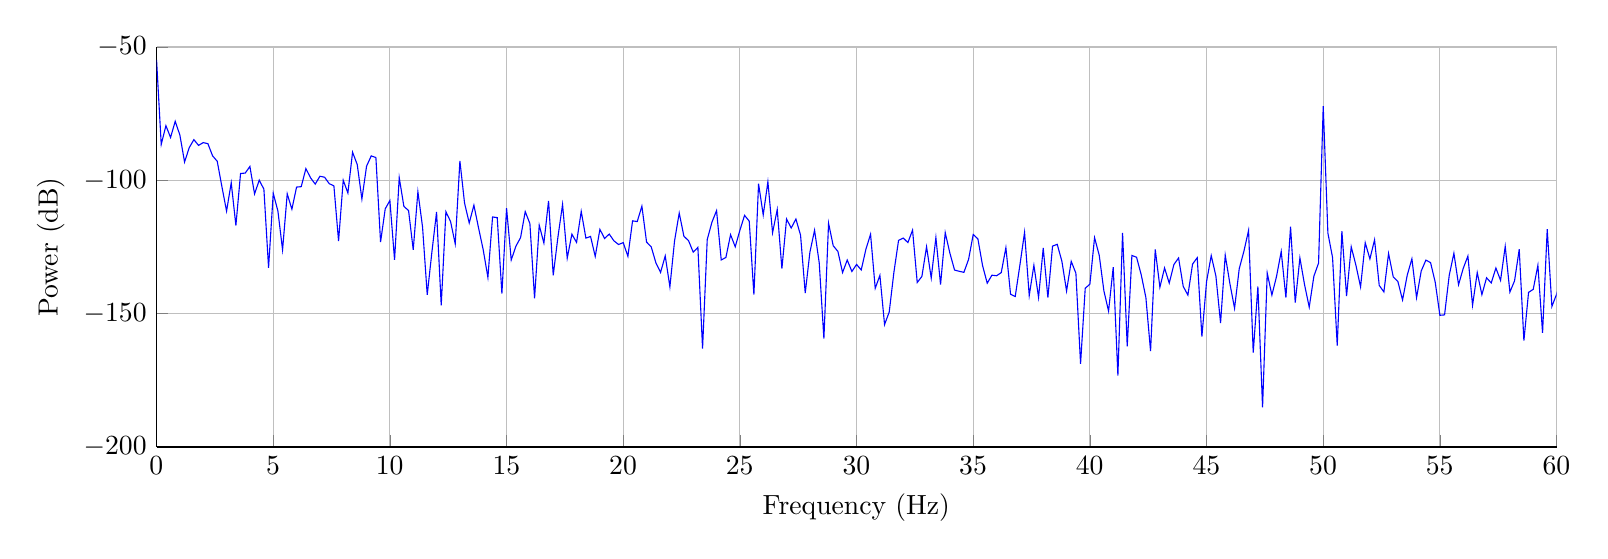
\begin{tikzpicture}

\begin{axis}[%
width=7in,
height=2in,
scale only axis,
xmin=0,
xmax=60,
xlabel={Frequency (Hz)},
xmajorgrids,
ymin=-200,
ymax=-50,
ylabel={Power (dB)},
ymajorgrids,
axis x line*=bottom,
axis y line*=left
]
\addplot [color=blue,solid,forget plot]
  table[row sep=crcr]{-600	-203.751610142527\\
-599.8	-145.966765539589\\
-599.6	-161.540975021055\\
-599.4	-163.513743631665\\
-599.2	-154.463163854512\\
-599	-145.343219882308\\
-598.8	-168.715748375528\\
-598.6	-156.160576712689\\
-598.4	-153.748160805267\\
-598.2	-161.299997795508\\
-598	-153.114430275644\\
-597.8	-154.198541753\\
-597.6	-144.064304085651\\
-597.4	-159.015475601499\\
-597.2	-154.373007362235\\
-597	-152.33939622831\\
-596.8	-150.174099505061\\
-596.6	-158.125574163909\\
-596.4	-162.325019182688\\
-596.2	-148.78935268225\\
-596	-166.307801648335\\
-595.8	-151.391342601624\\
-595.6	-166.757873286703\\
-595.4	-154.522384371746\\
-595.2	-155.001809659477\\
-595	-177.623917115685\\
-594.8	-148.954758160506\\
-594.6	-154.758784707954\\
-594.4	-157.305481717164\\
-594.2	-152.157575957394\\
-594	-161.453782128855\\
-593.8	-155.305786700146\\
-593.6	-159.66679872185\\
-593.4	-168.043455467947\\
-593.2	-148.77682032834\\
-593	-181.528515635405\\
-592.8	-149.795850887321\\
-592.6	-160.846598048148\\
-592.4	-170.334769224694\\
-592.2	-157.313962707296\\
-592	-143.996449832963\\
-591.8	-166.491119172475\\
-591.6	-190.827643446083\\
-591.4	-150.006820226714\\
-591.2	-153.453852336676\\
-591	-167.251143295399\\
-590.8	-164.080735476254\\
-590.6	-178.633498401557\\
-590.4	-147.3138392194\\
-590.2	-160.824413973326\\
-590	-153.491033620242\\
-589.8	-168.732580137233\\
-589.6	-151.537717761994\\
-589.4	-168.785939490883\\
-589.2	-177.251161929089\\
-589	-160.582581678476\\
-588.8	-169.28532455394\\
-588.6	-154.235333119029\\
-588.4	-154.256292045719\\
-588.2	-152.486360768635\\
-588	-152.257675551581\\
-587.8	-154.249169592985\\
-587.6	-151.838887205389\\
-587.4	-147.988766823179\\
-587.2	-179.188886950206\\
-587	-150.102804008456\\
-586.8	-155.509528023902\\
-586.6	-163.652703468042\\
-586.4	-156.614913576972\\
-586.2	-161.651160393935\\
-586	-169.105640886863\\
-585.8	-151.32202071552\\
-585.6	-147.874445555148\\
-585.4	-151.260316640203\\
-585.2	-158.389375346196\\
-585	-169.338041750058\\
-584.8	-145.075028533171\\
-584.6	-163.894067547454\\
-584.4	-162.191206975497\\
-584.2	-174.185683115542\\
-584	-155.774831857225\\
-583.8	-159.818925567015\\
-583.6	-153.225802454012\\
-583.4	-170.687065223346\\
-583.2	-160.380875469218\\
-583	-171.586251815544\\
-582.8	-177.155600835543\\
-582.6	-187.514082286353\\
-582.4	-156.963442817995\\
-582.2	-150.644819106911\\
-582	-164.302627432926\\
-581.8	-156.214890753229\\
-581.6	-155.874996141838\\
-581.4	-162.722206169004\\
-581.2	-146.44249492638\\
-581	-148.677119797357\\
-580.8	-163.439851791046\\
-580.6	-166.776654323765\\
-580.4	-161.750364184541\\
-580.2	-184.841608153161\\
-580	-165.68940679087\\
-579.8	-203.01242969306\\
-579.6	-149.753677562273\\
-579.4	-160.496588304463\\
-579.2	-156.5417780461\\
-579	-160.122819030803\\
-578.8	-161.966828706717\\
-578.6	-146.033240202925\\
-578.4	-151.803209052819\\
-578.2	-167.449408092912\\
-578	-163.357692591935\\
-577.8	-161.349184587302\\
-577.6	-152.733674829515\\
-577.4	-152.965629897443\\
-577.2	-151.07853469151\\
-577	-152.454907788192\\
-576.8	-175.686156755053\\
-576.6	-188.384617470606\\
-576.4	-153.876428927431\\
-576.2	-175.382884097511\\
-576	-159.352837336815\\
-575.8	-149.901531322914\\
-575.6	-156.186058953422\\
-575.4	-147.664092213171\\
-575.2	-151.483746401993\\
-575	-143.721663735052\\
-574.8	-154.648253823966\\
-574.6	-162.639739717842\\
-574.4	-151.246215316274\\
-574.2	-180.827203095843\\
-574	-162.586833187763\\
-573.8	-181.817105461834\\
-573.6	-163.063912773586\\
-573.4	-145.774084341118\\
-573.2	-172.247461156221\\
-573	-175.662409629814\\
-572.8	-165.106580280097\\
-572.6	-148.92749892933\\
-572.4	-149.889950950157\\
-572.2	-155.276757434984\\
-572	-147.730430492267\\
-571.8	-140.66710720083\\
-571.6	-178.561113101225\\
-571.4	-150.701992074004\\
-571.2	-147.90074585357\\
-571	-174.114533714913\\
-570.8	-140.572925765852\\
-570.6	-149.088998717495\\
-570.4	-155.86809826023\\
-570.2	-167.75872047875\\
-570	-158.281362612916\\
-569.8	-162.71788791051\\
-569.6	-152.689485939792\\
-569.4	-160.51124922117\\
-569.2	-154.148979705254\\
-569	-166.191042871412\\
-568.8	-156.698609111193\\
-568.6	-176.062964604625\\
-568.4	-156.469406870823\\
-568.2	-145.334503552874\\
-568	-151.095555594831\\
-567.8	-154.890953794804\\
-567.6	-161.123854528738\\
-567.4	-150.457014220757\\
-567.2	-158.230815018966\\
-567	-144.993736058806\\
-566.8	-161.954352204906\\
-566.6	-152.408717150784\\
-566.4	-171.581277176593\\
-566.2	-177.68669209339\\
-566	-151.796271353591\\
-565.8	-153.559105174839\\
-565.6	-159.07856661103\\
-565.4	-143.955188906307\\
-565.2	-154.251139596643\\
-565	-148.503353844051\\
-564.8	-149.651381368366\\
-564.6	-171.989738026594\\
-564.4	-177.030566510048\\
-564.2	-149.918229660669\\
-564	-177.722039085751\\
-563.8	-178.04368716628\\
-563.6	-149.991524796871\\
-563.4	-151.115658575712\\
-563.2	-151.691549755027\\
-563	-161.455857459941\\
-562.8	-158.738914742542\\
-562.6	-185.19017850494\\
-562.4	-168.797709838913\\
-562.2	-166.026145454688\\
-562	-166.711050994004\\
-561.8	-143.121881854823\\
-561.6	-158.678745591049\\
-561.4	-160.929963166331\\
-561.2	-143.955773903242\\
-561	-164.455243706932\\
-560.8	-169.970130573444\\
-560.6	-157.87477382889\\
-560.4	-155.473973494092\\
-560.2	-184.589603361564\\
-560	-159.914424626882\\
-559.8	-146.56359369262\\
-559.6	-141.749103212386\\
-559.4	-162.077881576816\\
-559.2	-156.446975428368\\
-559	-161.072747870138\\
-558.8	-177.829352573418\\
-558.6	-140.615036328525\\
-558.4	-158.231085322609\\
-558.2	-156.923805572109\\
-558	-144.320612790208\\
-557.8	-146.866760344714\\
-557.6	-160.526989054749\\
-557.4	-165.913975163233\\
-557.2	-171.525608302377\\
-557	-160.25147145442\\
-556.8	-153.661772676992\\
-556.6	-158.713009756308\\
-556.4	-156.815700976662\\
-556.2	-151.422087430655\\
-556	-166.51896444433\\
-555.8	-160.991465964095\\
-555.6	-153.002425793649\\
-555.4	-150.696384128686\\
-555.2	-173.655557169856\\
-555	-150.010830773846\\
-554.8	-188.451753942421\\
-554.6	-153.995392993135\\
-554.4	-153.366643874906\\
-554.2	-155.933415865541\\
-554	-207.939601864834\\
-553.8	-171.067252782046\\
-553.6	-169.524845534258\\
-553.4	-148.996944862835\\
-553.2	-160.554034016639\\
-553	-146.790968332533\\
-552.8	-147.927491977783\\
-552.6	-147.127104428063\\
-552.4	-146.47773734363\\
-552.2	-155.187145237064\\
-552	-154.535051620763\\
-551.8	-151.920406698281\\
-551.6	-148.272473996768\\
-551.4	-159.943935960579\\
-551.2	-160.659490421048\\
-551	-151.005285518014\\
-550.8	-158.298309985117\\
-550.6	-165.81401865981\\
-550.4	-155.589551772537\\
-550.2	-133.298389572462\\
-550	-158.485063068915\\
-549.8	-138.296768241038\\
-549.6	-140.953474072269\\
-549.4	-150.606309947885\\
-549.2	-141.892924838417\\
-549	-153.917527331224\\
-548.8	-155.823752355438\\
-548.6	-165.77407550408\\
-548.4	-142.028770336426\\
-548.2	-142.347047126132\\
-548	-158.161777574768\\
-547.8	-185.880113869801\\
-547.6	-148.502200563539\\
-547.4	-157.063791458672\\
-547.2	-148.106338232665\\
-547	-151.853618833781\\
-546.8	-166.660149425457\\
-546.6	-149.635059019726\\
-546.4	-146.191511648172\\
-546.2	-144.784683129275\\
-546	-176.166929683478\\
-545.8	-166.829280131651\\
-545.6	-147.466297469269\\
-545.4	-149.033541488422\\
-545.2	-152.31726843632\\
-545	-145.685217240883\\
-544.8	-163.327177286693\\
-544.6	-166.156427863158\\
-544.4	-163.496702497013\\
-544.2	-158.278953590015\\
-544	-156.4089150098\\
-543.8	-161.586459573218\\
-543.6	-156.384750631144\\
-543.4	-150.036987227378\\
-543.2	-147.073523144051\\
-543	-157.787408701032\\
-542.8	-155.443990283739\\
-542.6	-145.820981646005\\
-542.4	-165.620615774474\\
-542.2	-164.1551093436\\
-542	-170.7047780112\\
-541.8	-163.026396890545\\
-541.6	-146.880101189676\\
-541.4	-146.752420915825\\
-541.2	-180.204363858714\\
-541	-153.125563396133\\
-540.8	-149.54950543943\\
-540.6	-160.518968447932\\
-540.4	-155.953398393658\\
-540.2	-161.737649489106\\
-540	-186.475577080301\\
-539.8	-154.125213730164\\
-539.6	-173.599760186887\\
-539.4	-143.120849344995\\
-539.2	-142.022103538314\\
-539	-151.014599978087\\
-538.8	-161.498949824698\\
-538.6	-151.634926806663\\
-538.4	-153.910784623686\\
-538.2	-139.879227825893\\
-538	-168.132537286914\\
-537.8	-171.225236522138\\
-537.6	-157.140567149509\\
-537.4	-162.992157116655\\
-537.2	-151.784053723926\\
-537	-158.383314241759\\
-536.8	-151.557758546348\\
-536.6	-157.631524261135\\
-536.4	-156.169473263543\\
-536.2	-150.531378233115\\
-536	-150.871228139015\\
-535.8	-149.570727565759\\
-535.6	-187.817951779649\\
-535.4	-153.758446194662\\
-535.2	-149.330745878737\\
-535	-153.421015030109\\
-534.8	-154.201096342263\\
-534.6	-161.268632255792\\
-534.4	-148.131743125788\\
-534.2	-151.981682514781\\
-534	-147.733791596271\\
-533.8	-159.554334526043\\
-533.6	-142.588894887546\\
-533.4	-151.443687725685\\
-533.2	-139.208074713844\\
-533	-156.575460427544\\
-532.8	-182.192008550406\\
-532.6	-142.225755329055\\
-532.4	-161.532481062992\\
-532.2	-146.957999832189\\
-532	-150.384167532083\\
-531.8	-157.290053712374\\
-531.6	-167.497884647143\\
-531.4	-149.632793328224\\
-531.2	-151.088338222241\\
-531	-161.750769144051\\
-530.8	-172.494111671268\\
-530.6	-158.478678831193\\
-530.4	-144.047557610936\\
-530.2	-155.909127558651\\
-530	-156.296910470069\\
-529.8	-144.752380137427\\
-529.6	-166.634124205237\\
-529.4	-161.414442061527\\
-529.2	-160.021181616071\\
-529	-175.549957348981\\
-528.8	-149.373995683891\\
-528.6	-162.774985579561\\
-528.4	-178.466309749211\\
-528.2	-140.158346986381\\
-528	-157.739963547249\\
-527.8	-170.899897258844\\
-527.6	-169.118713067879\\
-527.4	-145.921262579466\\
-527.2	-169.787082058601\\
-527	-159.730589361368\\
-526.8	-147.295398949438\\
-526.6	-172.877186845612\\
-526.4	-172.627792885703\\
-526.2	-148.673535008282\\
-526	-154.812942482518\\
-525.8	-164.007228725974\\
-525.6	-159.300363757789\\
-525.4	-153.671248660019\\
-525.2	-173.481693696385\\
-525	-153.901141748395\\
-524.8	-170.377878577444\\
-524.6	-170.108768560687\\
-524.4	-157.443953639373\\
-524.2	-160.508974088184\\
-524	-149.182891135165\\
-523.8	-148.958911294397\\
-523.6	-163.212142637186\\
-523.4	-162.791121270849\\
-523.2	-149.422998286309\\
-523	-152.067373338492\\
-522.8	-158.158265895605\\
-522.6	-160.328892005772\\
-522.4	-159.422472555447\\
-522.2	-147.772413975284\\
-522	-153.408828776271\\
-521.8	-182.94601525149\\
-521.6	-142.26457358522\\
-521.4	-152.500147927264\\
-521.2	-136.991816859394\\
-521	-171.87503700539\\
-520.8	-156.294280120528\\
-520.6	-160.349765223004\\
-520.4	-169.717358239413\\
-520.2	-151.094766784514\\
-520	-181.448756811581\\
-519.8	-149.680183848745\\
-519.6	-150.749549219277\\
-519.4	-162.77490710175\\
-519.2	-173.903322696688\\
-519	-148.872708962665\\
-518.8	-176.217302735771\\
-518.6	-155.163488522931\\
-518.4	-148.351208431538\\
-518.2	-177.024646316501\\
-518	-169.201795204755\\
-517.8	-183.241250188726\\
-517.6	-184.169740333293\\
-517.4	-155.434053498586\\
-517.2	-152.515584610281\\
-517	-150.82640901016\\
-516.8	-147.434699616359\\
-516.6	-145.967193225122\\
-516.4	-168.739198518489\\
-516.2	-173.784159945754\\
-516	-154.250357800175\\
-515.8	-150.360651590514\\
-515.6	-154.765025775728\\
-515.4	-141.451658666219\\
-515.2	-137.525884944783\\
-515	-160.756353252212\\
-514.8	-155.39852900306\\
-514.6	-139.460923927851\\
-514.4	-147.725132697485\\
-514.2	-152.837890769857\\
-514	-168.188184815782\\
-513.8	-161.75656980663\\
-513.6	-156.049669458612\\
-513.4	-165.09675923383\\
-513.2	-171.262222747642\\
-513	-178.117590272851\\
-512.8	-139.536852293214\\
-512.6	-161.972696157778\\
-512.4	-170.287658690488\\
-512.2	-179.166101513824\\
-512	-184.866175116284\\
-511.8	-152.067471643615\\
-511.6	-158.006167379905\\
-511.4	-166.740899607162\\
-511.2	-166.793541369998\\
-511	-148.438209639285\\
-510.8	-167.127972072922\\
-510.6	-150.419507977483\\
-510.4	-148.466185412033\\
-510.2	-148.87251002219\\
-510	-148.379299967777\\
-509.8	-159.52893265507\\
-509.6	-150.811870676254\\
-509.4	-155.748718635469\\
-509.2	-173.350975212673\\
-509	-153.760654114349\\
-508.8	-153.291194898194\\
-508.6	-158.485701376979\\
-508.4	-170.586356236089\\
-508.2	-142.757758093027\\
-508	-143.166528520918\\
-507.8	-144.299819966396\\
-507.6	-164.625436041827\\
-507.4	-148.850909028078\\
-507.2	-163.08030645734\\
-507	-169.227579477157\\
-506.8	-139.794955523486\\
-506.6	-162.061285462644\\
-506.4	-156.994767643536\\
-506.2	-159.991511102327\\
-506	-171.986090914398\\
-505.8	-159.797786496305\\
-505.6	-157.551532181068\\
-505.4	-159.565902427387\\
-505.2	-145.335613110316\\
-505	-167.891705816948\\
-504.8	-159.741656646635\\
-504.6	-153.633201980586\\
-504.4	-150.236278754641\\
-504.2	-147.130059522755\\
-504	-153.38605713171\\
-503.8	-153.057615956837\\
-503.6	-145.30705875094\\
-503.4	-152.564860921499\\
-503.2	-151.993134015899\\
-503	-162.611033265184\\
-502.8	-150.025390408697\\
-502.6	-150.048890193315\\
-502.4	-170.013776828372\\
-502.2	-171.363737613027\\
-502	-153.766503944475\\
-501.8	-141.995314673352\\
-501.6	-155.122850666743\\
-501.4	-160.217391559787\\
-501.2	-147.577781910766\\
-501	-143.292125841289\\
-500.8	-148.172380465606\\
-500.6	-152.399522873787\\
-500.4	-188.569244053963\\
-500.2	-163.081812745329\\
-500	-155.405659789667\\
-499.8	-145.296760382099\\
-499.6	-194.9905578087\\
-499.4	-150.607470865019\\
-499.2	-144.792570862278\\
-499	-147.025005014009\\
-498.8	-159.988374212801\\
-498.6	-152.46437247838\\
-498.4	-148.121728905772\\
-498.2	-154.764426427163\\
-498	-152.090761225871\\
-497.8	-150.245767686243\\
-497.6	-184.097786066393\\
-497.4	-151.027599517635\\
-497.2	-147.647845409048\\
-497	-179.028022215869\\
-496.8	-189.201101944334\\
-496.6	-162.897455665153\\
-496.4	-154.182106552321\\
-496.2	-160.107924876536\\
-496	-146.515024100652\\
-495.8	-143.892558564974\\
-495.6	-164.449823346357\\
-495.4	-158.342158558096\\
-495.2	-156.852991999194\\
-495	-163.764526611918\\
-494.8	-155.062996306337\\
-494.6	-151.426069445038\\
-494.4	-147.16685246614\\
-494.2	-154.349153312618\\
-494	-155.920620137176\\
-493.8	-157.883255966148\\
-493.6	-146.714374700154\\
-493.4	-156.381587876404\\
-493.2	-155.614688931672\\
-493	-146.872484847368\\
-492.8	-152.14811467642\\
-492.6	-155.086326086371\\
-492.4	-162.691436975373\\
-492.2	-141.74618976544\\
-492	-159.283046317101\\
-491.8	-135.918416645715\\
-491.6	-143.685865083299\\
-491.4	-147.544795157175\\
-491.2	-170.786463852518\\
-491	-148.27728181421\\
-490.8	-178.504484324693\\
-490.6	-180.247239580637\\
-490.4	-163.780738744453\\
-490.2	-149.912972087618\\
-490	-148.163096794149\\
-489.8	-141.988589751972\\
-489.6	-183.710469826308\\
-489.4	-161.804844790276\\
-489.2	-181.055934235503\\
-489	-164.55998144965\\
-488.8	-148.241394965832\\
-488.6	-194.188191664472\\
-488.4	-167.834129658538\\
-488.2	-158.244294714348\\
-488	-136.600859474601\\
-487.8	-155.802855528752\\
-487.6	-155.187321226272\\
-487.4	-162.378426461692\\
-487.2	-161.825894699267\\
-487	-142.717621955175\\
-486.8	-165.141814735117\\
-486.6	-134.281408336378\\
-486.4	-142.531556171274\\
-486.2	-162.230727095851\\
-486	-160.353850259434\\
-485.8	-155.03350988293\\
-485.6	-157.343790171367\\
-485.4	-163.797636585764\\
-485.2	-159.209797315914\\
-485	-155.767277869498\\
-484.8	-165.181552917069\\
-484.6	-169.288322718358\\
-484.4	-151.871406673035\\
-484.2	-161.865407535574\\
-484	-145.043620378589\\
-483.8	-158.587233619885\\
-483.6	-166.088765733597\\
-483.4	-162.826153004173\\
-483.2	-147.172746956206\\
-483	-141.682576721701\\
-482.8	-156.005850796713\\
-482.6	-169.866752979998\\
-482.4	-157.367382447619\\
-482.2	-150.860418209461\\
-482	-172.599144277778\\
-481.8	-168.268230447025\\
-481.6	-170.045138302019\\
-481.4	-165.825182855115\\
-481.2	-144.269886980545\\
-481	-154.584441664214\\
-480.8	-150.477300623449\\
-480.6	-153.123625496836\\
-480.4	-158.398055822536\\
-480.2	-147.355542070177\\
-480	-174.368475226441\\
-479.8	-157.372406864296\\
-479.6	-148.433553813319\\
-479.4	-147.69350030199\\
-479.2	-150.84692054058\\
-479	-156.954425450577\\
-478.8	-153.433040031863\\
-478.6	-156.813362585596\\
-478.4	-140.06285397975\\
-478.2	-186.71218899738\\
-478	-153.684899683745\\
-477.8	-154.208455472464\\
-477.6	-144.75771544162\\
-477.4	-171.533288881405\\
-477.2	-156.010866540641\\
-477	-146.90131681567\\
-476.8	-156.092385962823\\
-476.6	-150.859878418716\\
-476.4	-144.762988322356\\
-476.2	-145.701798715019\\
-476	-156.692630867477\\
-475.8	-156.282906213001\\
-475.6	-151.002393111994\\
-475.4	-146.712469404694\\
-475.2	-164.310237041491\\
-475	-166.248045318077\\
-474.8	-144.065119194596\\
-474.6	-148.918118648206\\
-474.4	-143.703803626377\\
-474.2	-179.646371372227\\
-474	-206.338385112199\\
-473.8	-158.195074695682\\
-473.6	-147.299304915027\\
-473.4	-152.75378782399\\
-473.2	-152.533550306115\\
-473	-140.969022715648\\
-472.8	-146.981288279532\\
-472.6	-158.57784428137\\
-472.4	-146.626162759847\\
-472.2	-150.621065960014\\
-472	-167.379650498518\\
-471.8	-156.085302410967\\
-471.6	-147.132383565838\\
-471.4	-154.520923183715\\
-471.2	-155.593875839733\\
-471	-144.079829485945\\
-470.8	-149.91996601665\\
-470.6	-147.804359479676\\
-470.4	-163.980035284898\\
-470.2	-142.585453668812\\
-470	-176.651633218285\\
-469.8	-153.458243535511\\
-469.6	-157.706769561655\\
-469.4	-164.034659128653\\
-469.2	-169.5136282719\\
-469	-148.264015452762\\
-468.8	-153.551519541704\\
-468.6	-150.563798898773\\
-468.4	-191.169197890243\\
-468.2	-147.719116993161\\
-468	-194.131719529913\\
-467.8	-173.479596416001\\
-467.6	-140.937053371905\\
-467.4	-168.289804516069\\
-467.2	-160.669052597875\\
-467	-154.881636106191\\
-466.8	-153.315939694167\\
-466.6	-149.415521223701\\
-466.4	-144.517997275792\\
-466.2	-155.523009345571\\
-466	-157.94429231383\\
-465.8	-156.058113994863\\
-465.6	-149.935914725228\\
-465.4	-159.687385488548\\
-465.2	-147.13554215078\\
-465	-150.006058050563\\
-464.8	-165.852358294617\\
-464.6	-152.825416652157\\
-464.4	-160.774002881955\\
-464.2	-148.617410255767\\
-464	-144.867071395792\\
-463.8	-152.476790091078\\
-463.6	-143.6703912976\\
-463.4	-156.902590687311\\
-463.2	-160.747769739608\\
-463	-154.686514055637\\
-462.8	-153.515600068308\\
-462.6	-179.148537890304\\
-462.4	-172.139481224608\\
-462.2	-172.532371990294\\
-462	-148.811849283022\\
-461.8	-141.827867685642\\
-461.6	-165.710636958332\\
-461.4	-215.025228102876\\
-461.2	-153.93854531598\\
-461	-146.360859184885\\
-460.8	-149.975415314689\\
-460.6	-152.486643492176\\
-460.4	-151.521945960824\\
-460.2	-162.713789166866\\
-460	-161.227690629446\\
-459.8	-152.634583486568\\
-459.6	-143.097125067375\\
-459.4	-150.691976137727\\
-459.2	-172.313186841242\\
-459	-163.061504818844\\
-458.8	-152.509468734604\\
-458.6	-153.344422370519\\
-458.4	-156.455398126994\\
-458.2	-147.018331931819\\
-458	-153.707063026037\\
-457.8	-163.707865569739\\
-457.6	-166.377045203743\\
-457.4	-168.77314129918\\
-457.2	-151.235438078886\\
-457	-144.005397849856\\
-456.8	-153.435154705839\\
-456.6	-151.764391470852\\
-456.4	-159.510762836564\\
-456.2	-137.404872810673\\
-456	-170.52801605634\\
-455.8	-159.755524059079\\
-455.6	-153.690791270949\\
-455.4	-155.899885171192\\
-455.2	-161.150813989438\\
-455	-160.369749228636\\
-454.8	-168.701502246956\\
-454.6	-152.634634616345\\
-454.4	-148.253825194616\\
-454.2	-151.499339658929\\
-454	-144.286560415752\\
-453.8	-156.039274637115\\
-453.6	-155.639775300119\\
-453.4	-152.563647536379\\
-453.2	-184.624538408595\\
-453	-169.945843019188\\
-452.8	-173.866319845608\\
-452.6	-179.295322804217\\
-452.4	-183.551717056443\\
-452.2	-171.64956417175\\
-452	-149.793943265311\\
-451.8	-158.011789331545\\
-451.6	-190.380982589101\\
-451.4	-152.729137928578\\
-451.2	-164.704010969187\\
-451	-151.089393014888\\
-450.8	-155.766519080726\\
-450.6	-167.906470359486\\
-450.4	-167.837670446601\\
-450.2	-144.717927847196\\
-450	-159.982794373353\\
-449.8	-148.729647452038\\
-449.6	-141.861105542047\\
-449.4	-143.577951631681\\
-449.2	-164.193045100449\\
-449	-178.092134238169\\
-448.8	-163.499702379536\\
-448.6	-141.122855240616\\
-448.4	-156.376060158929\\
-448.2	-152.076394728845\\
-448	-145.927513154963\\
-447.8	-145.731633960388\\
-447.6	-183.397521574778\\
-447.4	-149.979058623472\\
-447.2	-156.272678027121\\
-447	-149.957885168528\\
-446.8	-154.247700408257\\
-446.6	-158.370171833991\\
-446.4	-148.985092035386\\
-446.2	-137.370145354174\\
-446	-158.912092421042\\
-445.8	-152.859648720074\\
-445.6	-174.497016169489\\
-445.4	-168.921522071741\\
-445.2	-165.489285961955\\
-445	-164.904493963936\\
-444.8	-159.253897524737\\
-444.6	-149.491377527577\\
-444.4	-153.886515065344\\
-444.2	-150.003805305342\\
-444	-148.690340155009\\
-443.8	-158.541255090237\\
-443.6	-161.792973091874\\
-443.4	-144.854365836154\\
-443.2	-172.51250066227\\
-443	-154.872376887763\\
-442.8	-147.59580667679\\
-442.6	-145.605720349641\\
-442.4	-151.447020182403\\
-442.2	-148.382250155328\\
-442	-148.175112959475\\
-441.8	-176.589537354543\\
-441.6	-159.586256677645\\
-441.4	-152.377598526607\\
-441.2	-159.899942262401\\
-441	-172.21294146927\\
-440.8	-146.955053434112\\
-440.6	-142.128723878964\\
-440.4	-153.107707145289\\
-440.2	-138.676276549158\\
-440	-160.990102244862\\
-439.8	-140.429254391346\\
-439.6	-153.838815649931\\
-439.4	-153.126562560149\\
-439.2	-152.440881070434\\
-439	-165.895960342446\\
-438.8	-163.751494254683\\
-438.6	-175.328877216131\\
-438.4	-148.489282530259\\
-438.2	-142.490666402286\\
-438	-147.336676291273\\
-437.8	-157.330058701779\\
-437.6	-190.708895152447\\
-437.4	-151.475292135142\\
-437.2	-153.04491093436\\
-437	-181.993171849471\\
-436.8	-138.305808341821\\
-436.6	-138.759753515831\\
-436.4	-168.201236924789\\
-436.2	-159.302508484994\\
-436	-157.089597110644\\
-435.8	-170.547741616423\\
-435.6	-142.793527690691\\
-435.4	-156.311057452989\\
-435.2	-160.474160866424\\
-435	-170.9845319174\\
-434.8	-150.354499621959\\
-434.6	-142.769836905718\\
-434.4	-182.661170766287\\
-434.2	-150.476125038473\\
-434	-145.492894530015\\
-433.8	-150.007595690849\\
-433.6	-176.87133440206\\
-433.4	-159.668724984265\\
-433.2	-149.694126221838\\
-433	-173.368868274424\\
-432.8	-142.844500732018\\
-432.6	-155.089403338241\\
-432.4	-153.107906452143\\
-432.2	-164.100659388692\\
-432	-165.881830655039\\
-431.8	-173.694261984003\\
-431.6	-149.682040693494\\
-431.4	-150.732790317216\\
-431.2	-166.305971852116\\
-431	-144.859560625639\\
-430.8	-183.39797848812\\
-430.6	-153.315226692221\\
-430.4	-144.375020702333\\
-430.2	-151.924432003441\\
-430	-195.937712526855\\
-429.8	-152.856163585463\\
-429.6	-171.520029009872\\
-429.4	-157.857091644789\\
-429.2	-140.819520701599\\
-429	-148.109289623835\\
-428.8	-160.069183172814\\
-428.6	-158.106963084753\\
-428.4	-185.637557360404\\
-428.2	-147.223684292908\\
-428	-154.055004645339\\
-427.8	-153.063639108998\\
-427.6	-156.151210088725\\
-427.4	-149.954106703758\\
-427.2	-162.22770545732\\
-427	-151.064533016135\\
-426.8	-144.678881255591\\
-426.6	-148.900943351559\\
-426.4	-177.490603755967\\
-426.2	-166.570297727325\\
-426	-150.337474997638\\
-425.8	-141.676867548101\\
-425.6	-167.745351312137\\
-425.4	-152.781181869656\\
-425.2	-177.954932708173\\
-425	-153.691209768739\\
-424.8	-143.692523469525\\
-424.6	-148.034384183491\\
-424.4	-151.735693274039\\
-424.2	-156.345747497713\\
-424	-156.68155080835\\
-423.8	-147.411043813095\\
-423.6	-172.984948285209\\
-423.4	-152.998782279906\\
-423.2	-153.114901655673\\
-423	-154.825492876921\\
-422.8	-140.765179331424\\
-422.6	-149.213308317066\\
-422.4	-152.406681994876\\
-422.2	-163.66291243755\\
-422	-162.666307000198\\
-421.8	-145.62853644087\\
-421.6	-156.640121375097\\
-421.4	-151.655056829368\\
-421.2	-171.398001280475\\
-421	-147.455537570567\\
-420.8	-142.531204337009\\
-420.6	-148.507439624888\\
-420.4	-155.852193673712\\
-420.2	-146.956125171701\\
-420	-145.910661435693\\
-419.8	-171.043812687588\\
-419.6	-150.499914709732\\
-419.4	-157.970301816066\\
-419.2	-141.890824494231\\
-419	-151.127388907553\\
-418.8	-159.310503157417\\
-418.6	-168.7174915311\\
-418.4	-156.109337556716\\
-418.2	-152.438130309332\\
-418	-156.904723491349\\
-417.8	-150.108202322478\\
-417.6	-142.061850604956\\
-417.4	-176.935359673747\\
-417.2	-155.42603151367\\
-417	-142.495062763183\\
-416.8	-161.315140362673\\
-416.6	-140.574200830466\\
-416.4	-175.834340387587\\
-416.2	-141.826346589439\\
-416	-162.650631366562\\
-415.8	-157.903589045947\\
-415.6	-152.267092368359\\
-415.4	-150.830245072751\\
-415.2	-154.431202884596\\
-415	-149.9237641597\\
-414.8	-187.319887278782\\
-414.6	-153.643402076299\\
-414.4	-148.019524673099\\
-414.2	-156.96196244873\\
-414	-141.892842145163\\
-413.8	-153.945249605264\\
-413.6	-157.788580441499\\
-413.4	-134.652825898834\\
-413.2	-143.181241179921\\
-413	-154.510768865882\\
-412.8	-167.122300700887\\
-412.6	-159.09584419388\\
-412.4	-150.436539282162\\
-412.2	-165.669917574613\\
-412	-162.249784297705\\
-411.8	-169.577316403054\\
-411.6	-149.370898689012\\
-411.4	-152.695432023232\\
-411.2	-151.067391596866\\
-411	-162.149255843905\\
-410.8	-169.22664613421\\
-410.6	-189.101806024406\\
-410.4	-145.945124447577\\
-410.2	-156.674379995135\\
-410	-158.362567185376\\
-409.8	-153.04155135978\\
-409.6	-141.420647957396\\
-409.4	-148.42079807825\\
-409.2	-165.646263472583\\
-409	-140.830192577434\\
-408.8	-153.401113405502\\
-408.6	-164.456654569213\\
-408.4	-160.251414668878\\
-408.2	-160.107922099027\\
-408	-146.517634263536\\
-407.8	-147.202393429884\\
-407.6	-140.969921875663\\
-407.4	-164.9438603674\\
-407.2	-155.658930068249\\
-407	-146.587401012985\\
-406.8	-160.355405502315\\
-406.6	-172.737678282268\\
-406.4	-177.217770109868\\
-406.2	-175.172691422867\\
-406	-170.017888946552\\
-405.8	-145.822813337308\\
-405.6	-181.695361812947\\
-405.4	-137.891647011267\\
-405.2	-152.207863249983\\
-405	-185.722631471608\\
-404.8	-142.581511793493\\
-404.6	-170.44339585011\\
-404.4	-160.024997915068\\
-404.2	-157.096751582329\\
-404	-146.424188336613\\
-403.8	-160.02074388567\\
-403.6	-153.444877140463\\
-403.4	-173.950695286179\\
-403.2	-149.67635021532\\
-403	-155.110578012052\\
-402.8	-155.491938493086\\
-402.6	-156.473092225085\\
-402.4	-153.316165082391\\
-402.2	-142.885895199958\\
-402	-161.492363757508\\
-401.8	-150.418346215255\\
-401.6	-152.678649156347\\
-401.4	-177.396573398636\\
-401.2	-156.59179648481\\
-401	-155.823168864479\\
-400.8	-184.727416808078\\
-400.6	-145.07005460321\\
-400.4	-146.694500245388\\
-400.2	-150.236476911689\\
-400	-146.626909637088\\
-399.8	-157.084046909485\\
-399.6	-162.6878872559\\
-399.4	-154.376927220284\\
-399.2	-147.591988825398\\
-399	-145.257374109468\\
-398.8	-153.081382142519\\
-398.6	-152.484930548416\\
-398.4	-147.57849689406\\
-398.2	-158.374705844189\\
-398	-138.783717601566\\
-397.8	-146.396418113971\\
-397.6	-153.923038308448\\
-397.4	-166.516827071862\\
-397.2	-174.770378855289\\
-397	-146.162649458928\\
-396.8	-145.77399979246\\
-396.6	-158.285358793893\\
-396.4	-147.134893604552\\
-396.2	-152.684708525092\\
-396	-154.485610440258\\
-395.8	-178.344495042559\\
-395.6	-142.722069446366\\
-395.4	-166.807494478094\\
-395.2	-157.855673878799\\
-395	-154.808149064465\\
-394.8	-165.371559882462\\
-394.6	-154.222176814719\\
-394.4	-140.906832041519\\
-394.2	-143.08056064825\\
-394	-146.106482886604\\
-393.8	-156.726243941314\\
-393.6	-146.391533154004\\
-393.4	-157.47218427659\\
-393.2	-156.396679317868\\
-393	-140.435938197224\\
-392.8	-136.614555369456\\
-392.6	-165.747296113095\\
-392.4	-149.17629710922\\
-392.2	-135.565947947356\\
-392	-155.589578713693\\
-391.8	-153.107703710925\\
-391.6	-156.744633994728\\
-391.4	-151.658161972936\\
-391.2	-178.10911025752\\
-391	-155.851430014187\\
-390.8	-156.841685869606\\
-390.6	-175.796724442151\\
-390.4	-139.554975285019\\
-390.2	-160.718606187688\\
-390	-166.313379313494\\
-389.8	-139.646894226701\\
-389.6	-154.246574797507\\
-389.4	-141.422271069493\\
-389.2	-153.958904839869\\
-389	-147.690660439185\\
-388.8	-159.395202127703\\
-388.6	-161.663258521951\\
-388.4	-169.004569161479\\
-388.2	-141.289942050005\\
-388	-148.868423596864\\
-387.8	-150.780506988916\\
-387.6	-156.869100030524\\
-387.4	-181.36744795617\\
-387.2	-165.703369027139\\
-387	-154.634232737849\\
-386.8	-211.403659674051\\
-386.6	-150.217939771655\\
-386.4	-155.505059939579\\
-386.2	-150.712776263177\\
-386	-136.841722808567\\
-385.8	-157.586922075009\\
-385.6	-155.369202548864\\
-385.4	-150.321561996975\\
-385.2	-157.431790879083\\
-385	-164.564335669752\\
-384.8	-148.884879868402\\
-384.6	-144.264143907856\\
-384.4	-155.399132458369\\
-384.2	-159.216915132686\\
-384	-169.195483702541\\
-383.8	-148.671908296136\\
-383.6	-144.936924753078\\
-383.4	-145.406815277983\\
-383.2	-160.220539990536\\
-383	-155.491451186707\\
-382.8	-160.578473628548\\
-382.6	-161.710813993099\\
-382.4	-149.766152936942\\
-382.2	-154.637883501123\\
-382	-149.315953314043\\
-381.8	-140.339945768468\\
-381.6	-170.357921233545\\
-381.4	-148.426050798296\\
-381.2	-172.542139440828\\
-381	-153.781100146479\\
-380.8	-162.666253008217\\
-380.6	-149.053643038402\\
-380.4	-148.967737328306\\
-380.2	-159.485978796172\\
-380	-138.594955462338\\
-379.8	-149.336945499708\\
-379.6	-146.995541013619\\
-379.4	-138.999429672557\\
-379.2	-147.473732506448\\
-379	-137.576711220454\\
-378.8	-148.466094406547\\
-378.6	-159.188340855918\\
-378.4	-150.121181316206\\
-378.2	-142.974570748076\\
-378	-144.499666180225\\
-377.8	-147.047552120049\\
-377.6	-142.336936336601\\
-377.4	-147.57755609369\\
-377.2	-151.469103562572\\
-377	-160.523077011212\\
-376.8	-185.899629488013\\
-376.6	-150.547728919359\\
-376.4	-156.553712343005\\
-376.2	-137.468865679495\\
-376	-155.089425307616\\
-375.8	-142.847892052179\\
-375.6	-154.664429127183\\
-375.4	-156.04487385122\\
-375.2	-147.123529957194\\
-375	-145.307203263086\\
-374.8	-153.115736985545\\
-374.6	-163.549407450555\\
-374.4	-159.248597761311\\
-374.2	-142.629091937368\\
-374	-166.255736368897\\
-373.8	-162.656205487274\\
-373.6	-172.481056873908\\
-373.4	-180.608099536798\\
-373.2	-159.300297031162\\
-373	-158.112125403848\\
-372.8	-175.814941919118\\
-372.6	-143.33171678617\\
-372.4	-176.687603322074\\
-372.2	-155.471879364477\\
-372	-143.53489790225\\
-371.8	-150.855970205165\\
-371.6	-144.583253178861\\
-371.4	-131.936938551984\\
-371.2	-152.155100989257\\
-371	-181.378783799353\\
-370.8	-174.120193857603\\
-370.6	-143.274048757559\\
-370.4	-145.791007529784\\
-370.2	-144.94736763409\\
-370	-171.298111044876\\
-369.8	-148.551769708675\\
-369.6	-157.64979329969\\
-369.4	-156.610849051742\\
-369.2	-152.364806861504\\
-369	-159.770953733981\\
-368.8	-177.505343044758\\
-368.6	-147.593730056682\\
-368.4	-144.596240412095\\
-368.2	-167.86039789928\\
-368	-144.17261207528\\
-367.8	-134.839961428158\\
-367.6	-134.661430241712\\
-367.4	-140.984077648645\\
-367.2	-155.930422707366\\
-367	-164.291148898421\\
-366.8	-147.320787957475\\
-366.6	-157.140999793446\\
-366.4	-148.41012807808\\
-366.2	-148.241572805462\\
-366	-159.182448544642\\
-365.8	-142.561107589976\\
-365.6	-146.446654207681\\
-365.4	-149.705570440857\\
-365.2	-149.696194647205\\
-365	-159.108533243447\\
-364.8	-161.740935487382\\
-364.6	-155.72730338174\\
-364.4	-142.754323584135\\
-364.2	-164.52058436858\\
-364	-156.137824803087\\
-363.8	-141.339390230564\\
-363.6	-156.094453140658\\
-363.4	-144.254360243136\\
-363.2	-152.405130581483\\
-363	-145.354001314608\\
-362.8	-155.467554002243\\
-362.6	-165.036273436915\\
-362.4	-162.950784039765\\
-362.2	-163.32857992693\\
-362	-144.331120038608\\
-361.8	-143.532574479675\\
-361.6	-141.321085714337\\
-361.4	-170.297147553537\\
-361.2	-150.574957049105\\
-361	-138.003541417832\\
-360.8	-149.086517957652\\
-360.6	-146.723498840467\\
-360.4	-160.494755501836\\
-360.2	-143.461823242549\\
-360	-150.646319948385\\
-359.8	-153.394706667236\\
-359.6	-169.529917616156\\
-359.4	-167.722860225205\\
-359.2	-141.786567923486\\
-359	-141.455932492601\\
-358.8	-150.511257570991\\
-358.6	-142.475208740897\\
-358.4	-144.553347332494\\
-358.2	-162.810863141234\\
-358	-157.383574856097\\
-357.8	-165.539365605841\\
-357.6	-143.129081963778\\
-357.4	-146.495617048025\\
-357.2	-151.989754090367\\
-357	-152.675682759441\\
-356.8	-145.622996141798\\
-356.6	-147.584919872881\\
-356.4	-147.071740574226\\
-356.2	-160.428324969914\\
-356	-152.251513097591\\
-355.8	-148.837066242491\\
-355.6	-145.551753393901\\
-355.4	-151.024774670133\\
-355.2	-133.963579176814\\
-355	-146.69189001088\\
-354.8	-145.166112457314\\
-354.6	-145.692475016988\\
-354.4	-148.438259392596\\
-354.2	-156.061854865044\\
-354	-148.895495833065\\
-353.8	-151.214639342009\\
-353.6	-156.478643208437\\
-353.4	-152.993943041842\\
-353.2	-159.935519503774\\
-353	-181.355243420071\\
-352.8	-157.848398703724\\
-352.6	-145.629281569498\\
-352.4	-143.707927716244\\
-352.2	-164.026259918259\\
-352	-141.955936182195\\
-351.8	-169.595574776822\\
-351.6	-138.708007859656\\
-351.4	-134.878808818512\\
-351.2	-155.030638363164\\
-351	-180.908258273507\\
-350.8	-154.114895471852\\
-350.6	-146.014301805118\\
-350.4	-149.586005511356\\
-350.2	-154.018164091473\\
-350	-153.709412159032\\
-349.8	-157.658460866422\\
-349.6	-145.409166343732\\
-349.4	-156.070546862912\\
-349.2	-159.969911737796\\
-349	-153.439845945793\\
-348.8	-150.70675215781\\
-348.6	-150.023265347326\\
-348.4	-145.47033728148\\
-348.2	-142.556710115316\\
-348	-153.304253782963\\
-347.8	-137.996726299016\\
-347.6	-143.213298017916\\
-347.4	-140.12589756815\\
-347.2	-148.97252126171\\
-347	-151.520114184077\\
-346.8	-151.207096540462\\
-346.6	-183.674551849233\\
-346.4	-155.854909697826\\
-346.2	-140.281306212143\\
-346	-158.137410205738\\
-345.8	-174.55368523745\\
-345.6	-155.616538417759\\
-345.4	-153.344333299931\\
-345.2	-143.368598021856\\
-345	-174.954714818106\\
-344.8	-148.871423308197\\
-344.6	-157.383583592895\\
-344.4	-145.957242804889\\
-344.2	-160.356838823677\\
-344	-144.253924410705\\
-343.8	-158.977626450902\\
-343.6	-162.042689362701\\
-343.4	-154.791148137821\\
-343.2	-144.089137583321\\
-343	-153.075757244224\\
-342.8	-142.435388038768\\
-342.6	-156.649484798036\\
-342.4	-137.86112509722\\
-342.2	-142.365278772514\\
-342	-148.349892970219\\
-341.8	-151.04409413916\\
-341.6	-150.501594984184\\
-341.4	-152.167293560981\\
-341.2	-153.648816266278\\
-341	-143.454966358946\\
-340.8	-155.089011069799\\
-340.6	-162.645032272314\\
-340.4	-141.781414862943\\
-340.2	-138.505306810139\\
-340	-169.778663027238\\
-339.8	-178.412899035322\\
-339.6	-152.978800902149\\
-339.4	-178.267182025842\\
-339.2	-157.765693917538\\
-339	-137.438155534731\\
-338.8	-151.992256538355\\
-338.6	-175.873052281449\\
-338.4	-152.121771782579\\
-338.2	-157.514148717717\\
-338	-144.369339769151\\
-337.8	-142.578527481063\\
-337.6	-140.600225534399\\
-337.4	-144.469359432564\\
-337.2	-144.66964379719\\
-337	-150.578152239144\\
-336.8	-142.983383287364\\
-336.6	-144.433685968389\\
-336.4	-163.343584126966\\
-336.2	-152.555936845562\\
-336	-166.539875317808\\
-335.8	-179.922263866908\\
-335.6	-158.580375936495\\
-335.4	-161.960200553488\\
-335.2	-140.799586193268\\
-335	-163.778739106359\\
-334.8	-149.570949103738\\
-334.6	-149.770911817244\\
-334.4	-152.330049666155\\
-334.2	-156.563587630308\\
-334	-142.114473630888\\
-333.8	-170.326200687206\\
-333.6	-165.347414100786\\
-333.4	-169.13077134176\\
-333.2	-142.889038085551\\
-333	-145.403180857132\\
-332.8	-151.846401568843\\
-332.6	-149.482371342198\\
-332.4	-159.103396006395\\
-332.2	-150.104071970233\\
-332	-157.59287454178\\
-331.8	-164.580805501558\\
-331.6	-175.089119491518\\
-331.4	-133.845466258701\\
-331.2	-149.660388707658\\
-331	-145.760847222423\\
-330.8	-176.635451429444\\
-330.6	-139.191243503011\\
-330.4	-135.096487588736\\
-330.2	-137.95309118291\\
-330	-148.144773125852\\
-329.8	-157.412009284191\\
-329.6	-160.127850083067\\
-329.4	-150.467680244038\\
-329.2	-160.395931656432\\
-329	-143.554472989232\\
-328.8	-148.729029637236\\
-328.6	-148.215790307923\\
-328.4	-141.987996494966\\
-328.2	-155.206357000216\\
-328	-159.876231273385\\
-327.8	-142.67795500183\\
-327.6	-161.392938500302\\
-327.4	-160.316139960943\\
-327.2	-139.831109183914\\
-327	-149.876337328129\\
-326.8	-159.579969116375\\
-326.6	-145.178064632889\\
-326.4	-146.127820315914\\
-326.2	-159.395100793077\\
-326	-147.597323433209\\
-325.8	-138.744021754722\\
-325.6	-138.967145439182\\
-325.4	-143.265438977971\\
-325.2	-204.845493409752\\
-325	-157.415002530521\\
-324.8	-188.003036309932\\
-324.6	-145.562169214993\\
-324.4	-145.074565722912\\
-324.2	-145.457902278303\\
-324	-170.59462146993\\
-323.8	-147.849572030919\\
-323.6	-158.214247235837\\
-323.4	-157.133214263436\\
-323.2	-142.09283257021\\
-323	-142.534100402682\\
-322.8	-142.647843384041\\
-322.6	-150.152699047155\\
-322.4	-144.934513923237\\
-322.2	-156.442033793229\\
-322	-146.190304480123\\
-321.8	-140.300633280617\\
-321.6	-140.507097574789\\
-321.4	-139.855833894135\\
-321.2	-161.862557811101\\
-321	-163.745973398164\\
-320.8	-142.374474812264\\
-320.6	-147.894030024854\\
-320.4	-139.712180190081\\
-320.2	-167.397678786438\\
-320	-146.365175194135\\
-319.8	-154.990769249011\\
-319.6	-142.259014208321\\
-319.4	-146.428345977991\\
-319.2	-151.667864426747\\
-319	-154.262026828523\\
-318.8	-153.73325593264\\
-318.6	-155.801138510999\\
-318.4	-147.33603997926\\
-318.2	-154.263624137629\\
-318	-171.240546431746\\
-317.8	-147.484210605872\\
-317.6	-143.678270842612\\
-317.4	-160.428428632497\\
-317.2	-135.033372849104\\
-317	-166.085506683693\\
-316.8	-164.51450498966\\
-316.6	-140.455087812278\\
-316.4	-156.770394408705\\
-316.2	-147.004053095424\\
-316	-141.284742667105\\
-315.8	-148.819016421281\\
-315.6	-148.411737192232\\
-315.4	-169.267241167916\\
-315.2	-150.654523826982\\
-315	-149.015818219741\\
-314.8	-159.401977006854\\
-314.6	-179.473780818041\\
-314.4	-159.475008286938\\
-314.2	-155.771152490659\\
-314	-140.243147971233\\
-313.8	-133.9035820962\\
-313.6	-160.419441478914\\
-313.4	-156.432038795813\\
-313.2	-149.48522112314\\
-313	-146.192041768049\\
-312.8	-142.639912009756\\
-312.6	-156.835043718193\\
-312.4	-149.58948906569\\
-312.2	-140.381734225025\\
-312	-156.055822242466\\
-311.8	-155.697078329785\\
-311.6	-146.683344348148\\
-311.4	-178.233149355449\\
-311.2	-150.478239504503\\
-311	-161.834616606279\\
-310.8	-172.890755201465\\
-310.6	-152.478148334166\\
-310.4	-149.648535075023\\
-310.2	-147.136111847016\\
-310	-161.018378939105\\
-309.8	-141.498947093511\\
-309.6	-143.920412910686\\
-309.4	-147.491871664247\\
-309.2	-145.371255294783\\
-309	-140.178336689781\\
-308.8	-149.09035747088\\
-308.6	-135.355592727632\\
-308.4	-137.8420788144\\
-308.2	-151.583624665939\\
-308	-141.016552326374\\
-307.8	-144.760535686262\\
-307.6	-202.017375199238\\
-307.4	-157.449062820805\\
-307.2	-151.602970959097\\
-307	-164.637038564197\\
-306.8	-140.520500090472\\
-306.6	-146.374585087889\\
-306.4	-169.451786690167\\
-306.2	-157.406654543126\\
-306	-147.290036802683\\
-305.8	-159.364222077932\\
-305.6	-145.97689781375\\
-305.4	-142.738836466215\\
-305.2	-183.402481921566\\
-305	-142.229730416084\\
-304.8	-143.019767270209\\
-304.6	-147.168688878862\\
-304.4	-166.843043228227\\
-304.2	-163.919074556621\\
-304	-141.476664809536\\
-303.8	-152.214615726434\\
-303.6	-156.061105194583\\
-303.4	-160.29331655979\\
-303.2	-171.412292834394\\
-303	-179.487939024889\\
-302.8	-139.633014936871\\
-302.6	-145.919580267976\\
-302.4	-160.161879934573\\
-302.2	-146.951843314644\\
-302	-150.657436022897\\
-301.8	-139.833893528037\\
-301.6	-150.289898317666\\
-301.4	-145.605823881867\\
-301.2	-142.479851415132\\
-301	-137.827523525494\\
-300.8	-173.337825701328\\
-300.6	-152.045484489079\\
-300.4	-164.512509036237\\
-300.2	-142.740325101596\\
-300	-135.917313094308\\
-299.8	-145.119755243515\\
-299.6	-146.501114455656\\
-299.4	-147.429506302944\\
-299.2	-160.826829633678\\
-299	-150.669415689236\\
-298.8	-150.623101370129\\
-298.6	-164.910286744132\\
-298.4	-146.281447607344\\
-298.2	-188.254260954192\\
-298	-158.586338449317\\
-297.8	-146.848601872438\\
-297.6	-148.53322000492\\
-297.4	-151.464532463539\\
-297.2	-171.237605003603\\
-297	-147.111284475392\\
-296.8	-149.204646499015\\
-296.6	-185.191189588158\\
-296.4	-141.430877020669\\
-296.2	-156.175149652943\\
-296	-148.702776918212\\
-295.8	-136.712078663722\\
-295.6	-138.68146475507\\
-295.4	-143.156116684469\\
-295.2	-142.669706528081\\
-295	-151.547495054581\\
-294.8	-148.235015105951\\
-294.6	-150.044498693393\\
-294.4	-139.653160553881\\
-294.2	-169.362984227474\\
-294	-148.755402974235\\
-293.8	-167.976227277346\\
-293.6	-143.205197396579\\
-293.4	-147.305023135661\\
-293.2	-146.310230854873\\
-293	-151.155878003502\\
-292.8	-152.408869155153\\
-292.6	-155.97015344456\\
-292.4	-136.034428096497\\
-292.2	-150.165815739875\\
-292	-139.019889456582\\
-291.8	-215.034387134422\\
-291.6	-168.060616663087\\
-291.4	-153.846188383999\\
-291.2	-166.931255936376\\
-291	-151.154610878672\\
-290.8	-140.731926418195\\
-290.6	-169.355432797464\\
-290.4	-146.117281038126\\
-290.2	-154.845426165537\\
-290	-135.427794526343\\
-289.8	-135.296855831999\\
-289.6	-167.124431629961\\
-289.4	-137.229859677754\\
-289.2	-139.647438332924\\
-289	-145.747236097991\\
-288.8	-136.376889710025\\
-288.6	-143.070870642918\\
-288.4	-149.195607736278\\
-288.2	-152.973051516333\\
-288	-148.098541963007\\
-287.8	-148.719338692121\\
-287.6	-139.580670403599\\
-287.4	-152.707895377207\\
-287.2	-147.580200954433\\
-287	-138.394476195229\\
-286.8	-144.653925737634\\
-286.6	-167.956644489406\\
-286.4	-135.277702961352\\
-286.2	-145.353043987187\\
-286	-156.029707463828\\
-285.8	-142.558020223799\\
-285.6	-152.74610005781\\
-285.4	-147.818692624698\\
-285.2	-165.333106619996\\
-285	-150.983554778988\\
-284.8	-150.368093487882\\
-284.6	-139.888047174408\\
-284.4	-150.816487150378\\
-284.2	-177.735469295579\\
-284	-159.445011682102\\
-283.8	-161.929135250159\\
-283.6	-141.911728697433\\
-283.4	-143.334939752771\\
-283.2	-140.49722908655\\
-283	-148.39738680567\\
-282.8	-140.712231402705\\
-282.6	-133.534385034976\\
-282.4	-144.363659342318\\
-282.2	-148.026114923831\\
-282	-150.95509660713\\
-281.8	-146.306383675602\\
-281.6	-140.075659327015\\
-281.4	-143.508582653207\\
-281.2	-149.484685475462\\
-281	-176.786184005316\\
-280.8	-135.364252215558\\
-280.6	-159.744816944998\\
-280.4	-152.876682900947\\
-280.2	-156.319110129799\\
-280	-145.491080266109\\
-279.8	-138.360188566232\\
-279.6	-153.0933985204\\
-279.4	-146.421965025825\\
-279.2	-148.387843486449\\
-279	-146.190291518019\\
-278.8	-145.572042603759\\
-278.6	-161.520227442329\\
-278.4	-144.766643907253\\
-278.2	-155.989456417915\\
-278	-169.034057293606\\
-277.8	-142.541892389216\\
-277.6	-182.70571637772\\
-277.4	-156.273108623423\\
-277.2	-137.149029745174\\
-277	-154.321983623099\\
-276.8	-144.09124532888\\
-276.6	-162.103910017148\\
-276.4	-148.531623531872\\
-276.2	-168.202837452033\\
-276	-139.391207435452\\
-275.8	-140.830753358277\\
-275.6	-151.245157794673\\
-275.4	-147.894032347221\\
-275.2	-142.424409003391\\
-275	-160.188774681539\\
-274.8	-148.492408527575\\
-274.6	-156.831349676951\\
-274.4	-143.137521304908\\
-274.2	-149.480115025314\\
-274	-153.97823740067\\
-273.8	-149.999466067013\\
-273.6	-145.315417961927\\
-273.4	-152.56459050777\\
-273.2	-150.766323597905\\
-273	-146.653281299752\\
-272.8	-143.298109432736\\
-272.6	-130.319828549604\\
-272.4	-151.779006850364\\
-272.2	-134.166136379295\\
-272	-151.183089143609\\
-271.8	-141.259691017614\\
-271.6	-150.523196393184\\
-271.4	-136.205354343475\\
-271.2	-142.931990477198\\
-271	-140.93212915949\\
-270.8	-150.401284081694\\
-270.6	-155.427286953567\\
-270.4	-169.727418693034\\
-270.2	-148.02783141115\\
-270	-148.244734257964\\
-269.8	-154.636493508732\\
-269.6	-136.289482893687\\
-269.4	-146.298686044478\\
-269.2	-130.221155419348\\
-269	-156.017476517823\\
-268.8	-147.699667351452\\
-268.6	-134.697797469499\\
-268.4	-139.563090349066\\
-268.2	-139.1534528661\\
-268	-149.334220125908\\
-267.8	-151.035323185328\\
-267.6	-151.133165148634\\
-267.4	-181.14531122798\\
-267.2	-144.929479546013\\
-267	-160.91258561613\\
-266.8	-147.086797286513\\
-266.6	-133.915191689423\\
-266.4	-157.688249386454\\
-266.2	-168.708603045269\\
-266	-146.898548361264\\
-265.8	-147.648033498547\\
-265.6	-143.188235618844\\
-265.4	-136.74554827859\\
-265.2	-139.187830422441\\
-265	-133.860129950173\\
-264.8	-155.609639763759\\
-264.6	-143.820081372185\\
-264.4	-152.739063411155\\
-264.2	-143.071412623167\\
-264	-142.005363113219\\
-263.8	-148.658353082061\\
-263.6	-157.718646658122\\
-263.4	-136.524754717919\\
-263.2	-143.189449403828\\
-263	-140.566144858819\\
-262.8	-151.104646605501\\
-262.6	-141.215750799458\\
-262.4	-170.521580955076\\
-262.2	-155.000475669048\\
-262	-136.265317321629\\
-261.8	-163.421024165452\\
-261.6	-145.692971645679\\
-261.4	-145.503164453095\\
-261.2	-139.282635332474\\
-261	-153.732346837212\\
-260.8	-157.254701723189\\
-260.6	-156.302119770032\\
-260.4	-151.148275510623\\
-260.2	-144.401029998478\\
-260	-144.151124571136\\
-259.8	-143.908443113979\\
-259.6	-163.50106926497\\
-259.4	-142.422960261635\\
-259.2	-144.845587812175\\
-259	-142.354323429854\\
-258.8	-162.335920006588\\
-258.6	-150.09634735498\\
-258.4	-163.393089699697\\
-258.2	-156.700413476306\\
-258	-149.099085577137\\
-257.8	-149.828849961365\\
-257.6	-169.499256709026\\
-257.4	-144.094388752551\\
-257.2	-136.846306805645\\
-257	-137.661363545135\\
-256.8	-156.512569694378\\
-256.6	-148.316372373724\\
-256.4	-164.309574325516\\
-256.2	-158.403344680005\\
-256	-139.147300767939\\
-255.8	-149.98726314974\\
-255.6	-139.873038662006\\
-255.4	-155.30135281339\\
-255.2	-139.587818591003\\
-255	-129.470616370097\\
-254.8	-150.552821619683\\
-254.6	-158.006457166043\\
-254.4	-132.974372423697\\
-254.2	-138.968949960815\\
-254	-148.814033954739\\
-253.8	-142.424974254143\\
-253.6	-153.809882059948\\
-253.4	-150.103609499954\\
-253.2	-137.79373463304\\
-253	-144.510013848998\\
-252.8	-137.960286226884\\
-252.6	-146.342977342385\\
-252.4	-138.455029108192\\
-252.2	-163.199087837048\\
-252	-138.544089015666\\
-251.8	-142.927490113453\\
-251.6	-157.124155917184\\
-251.4	-132.350439814918\\
-251.2	-149.620678118023\\
-251	-138.215041891474\\
-250.8	-150.609883789221\\
-250.6	-142.690418112752\\
-250.4	-152.42493700363\\
-250.2	-135.135747225202\\
-250	-125.246484061636\\
-249.8	-133.253544067\\
-249.6	-133.402441212409\\
-249.4	-156.498729544942\\
-249.2	-144.41615036069\\
-249	-147.430721685767\\
-248.8	-148.346600132571\\
-248.6	-156.4195719628\\
-248.4	-169.867778185781\\
-248.2	-147.115268882647\\
-248	-145.03611461987\\
-247.8	-155.822021552764\\
-247.6	-140.927913412814\\
-247.4	-161.073861202505\\
-247.2	-141.770308172773\\
-247	-153.916197454674\\
-246.8	-155.750598688836\\
-246.6	-151.055794238789\\
-246.4	-141.734202152889\\
-246.2	-135.274161536003\\
-246	-135.729874702163\\
-245.8	-144.373984881124\\
-245.6	-153.955303830189\\
-245.4	-138.158811757106\\
-245.2	-157.084077194915\\
-245	-150.029326455236\\
-244.8	-132.994520928105\\
-244.6	-146.848031514223\\
-244.4	-153.76289361252\\
-244.2	-174.869822934617\\
-244	-145.056348449969\\
-243.8	-170.538931461483\\
-243.6	-158.020361799399\\
-243.4	-158.595925459872\\
-243.2	-151.400881707519\\
-243	-142.672262012559\\
-242.8	-202.508631949662\\
-242.6	-162.865822773247\\
-242.4	-141.42235033543\\
-242.2	-132.566816421533\\
-242	-148.844295002238\\
-241.8	-146.633713601286\\
-241.6	-154.430260492391\\
-241.4	-176.344409700362\\
-241.2	-165.391716480715\\
-241	-154.287526907838\\
-240.8	-145.811739659435\\
-240.6	-155.002181516165\\
-240.4	-159.138864234868\\
-240.2	-152.137794661126\\
-240	-140.881521840214\\
-239.8	-156.738574046141\\
-239.6	-133.18554343871\\
-239.4	-142.940443921418\\
-239.2	-131.37304170532\\
-239	-135.567921391032\\
-238.8	-140.951933519142\\
-238.6	-141.630202051527\\
-238.4	-142.244295246998\\
-238.2	-134.004200307182\\
-238	-137.106211785317\\
-237.8	-151.840368317505\\
-237.6	-152.061008080791\\
-237.4	-135.760915278123\\
-237.2	-139.558507583807\\
-237	-143.779859812079\\
-236.8	-170.277584173606\\
-236.6	-142.950489832911\\
-236.4	-141.730115835197\\
-236.2	-144.353759072298\\
-236	-154.948148892466\\
-235.8	-151.490081713999\\
-235.6	-187.547049219977\\
-235.4	-149.569241374469\\
-235.2	-151.500971107198\\
-235	-157.168011590274\\
-234.8	-152.12688820537\\
-234.6	-133.214402319093\\
-234.4	-152.24728861542\\
-234.2	-157.845382894789\\
-234	-144.282874352613\\
-233.8	-158.416173642817\\
-233.6	-145.705575669663\\
-233.4	-156.864203491626\\
-233.2	-133.352493233774\\
-233	-137.896271090436\\
-232.8	-135.877086817615\\
-232.6	-143.923911747258\\
-232.4	-142.996656425246\\
-232.2	-146.447686689122\\
-232	-157.327549910717\\
-231.8	-149.029208861827\\
-231.6	-156.979055700939\\
-231.4	-140.907125947643\\
-231.2	-130.704562416422\\
-231	-142.770638635811\\
-230.8	-150.33860617578\\
-230.6	-140.652452580327\\
-230.4	-134.286108498398\\
-230.2	-134.294674704892\\
-230	-141.413874785436\\
-229.8	-144.140269036327\\
-229.6	-144.671631573953\\
-229.4	-138.643873471168\\
-229.2	-140.771316774093\\
-229	-147.586485327227\\
-228.8	-139.504707930602\\
-228.6	-150.00393223616\\
-228.4	-197.91718678268\\
-228.2	-146.857916903108\\
-228	-170.982532829896\\
-227.8	-138.373961032507\\
-227.6	-141.846967371652\\
-227.4	-135.176774613776\\
-227.2	-141.420620942882\\
-227	-145.879429544041\\
-226.8	-132.129848763356\\
-226.6	-144.020444085961\\
-226.4	-152.385871638334\\
-226.2	-141.012671839059\\
-226	-149.051152591087\\
-225.8	-135.100119338991\\
-225.6	-165.026740575763\\
-225.4	-144.167339409792\\
-225.2	-139.807285984428\\
-225	-153.497397279432\\
-224.8	-142.517805415427\\
-224.6	-153.590144777723\\
-224.4	-152.379962204828\\
-224.2	-135.266902437039\\
-224	-149.225023364538\\
-223.8	-144.868309355789\\
-223.6	-147.419914454039\\
-223.4	-138.786137599895\\
-223.2	-134.233127762025\\
-223	-130.260692131562\\
-222.8	-145.944159111599\\
-222.6	-139.546979494648\\
-222.4	-147.278603361137\\
-222.2	-154.102808285705\\
-222	-162.573049460713\\
-221.8	-167.991987484365\\
-221.6	-162.597338039075\\
-221.4	-140.542026397899\\
-221.2	-147.204525179524\\
-221	-160.30250569053\\
-220.8	-160.887234432243\\
-220.6	-153.14063697848\\
-220.4	-142.13854780849\\
-220.2	-143.933404908614\\
-220	-142.700271184861\\
-219.8	-145.410207128967\\
-219.6	-150.665831851041\\
-219.4	-133.724787094899\\
-219.2	-147.251904565467\\
-219	-136.118959438768\\
-218.8	-143.305006085068\\
-218.6	-176.024584671588\\
-218.4	-172.841533290683\\
-218.2	-160.787684660856\\
-218	-137.740393658127\\
-217.8	-146.507623685206\\
-217.6	-149.874639863104\\
-217.4	-148.563888876176\\
-217.2	-139.856851895049\\
-217	-136.445189489033\\
-216.8	-142.982139465959\\
-216.6	-124.201598151781\\
-216.4	-139.641512983464\\
-216.2	-150.199388384721\\
-216	-144.936365035509\\
-215.8	-155.741775664935\\
-215.6	-138.973235513798\\
-215.4	-145.245181280194\\
-215.2	-140.976425436304\\
-215	-141.248669807937\\
-214.8	-143.919029971232\\
-214.6	-152.675493699335\\
-214.4	-141.826406974857\\
-214.2	-139.074869412464\\
-214	-143.475716660713\\
-213.8	-157.940497006769\\
-213.6	-128.17651357835\\
-213.4	-151.361149503588\\
-213.2	-136.281859638532\\
-213	-132.865630804831\\
-212.8	-139.787759131027\\
-212.6	-145.474951096463\\
-212.4	-150.676338222105\\
-212.2	-145.270646987005\\
-212	-140.835538247929\\
-211.8	-136.899619138141\\
-211.6	-153.716385688444\\
-211.4	-143.05679066108\\
-211.2	-155.73210918427\\
-211	-140.289773904076\\
-210.8	-147.750043109969\\
-210.6	-136.181026199957\\
-210.4	-136.392737646481\\
-210.2	-153.215575774378\\
-210	-145.326905417835\\
-209.8	-134.801556960253\\
-209.6	-156.062135688849\\
-209.4	-150.546816694579\\
-209.2	-141.882592742936\\
-209	-153.495666859272\\
-208.8	-147.626120628292\\
-208.6	-133.438155581709\\
-208.4	-144.310948318068\\
-208.2	-129.784546807097\\
-208	-147.644544480797\\
-207.8	-138.958280423936\\
-207.6	-150.440350413163\\
-207.4	-138.364285017361\\
-207.2	-149.58489149926\\
-207	-158.140404588885\\
-206.8	-176.741027537471\\
-206.6	-141.304118490469\\
-206.4	-145.889674185444\\
-206.2	-161.463460378943\\
-206	-157.865942862225\\
-205.8	-156.351975797469\\
-205.6	-137.007175285899\\
-205.4	-141.301233147546\\
-205.2	-153.552557934466\\
-205	-170.906564778965\\
-204.8	-143.007948515702\\
-204.6	-149.966011893048\\
-204.4	-133.799231966061\\
-204.2	-131.06327184392\\
-204	-154.1466741898\\
-203.8	-143.103137170176\\
-203.6	-138.33044968923\\
-203.4	-146.236701384569\\
-203.2	-143.477481073939\\
-203	-155.775253035129\\
-202.8	-146.900151710273\\
-202.6	-180.043010251076\\
-202.4	-150.224995602241\\
-202.2	-142.40577238912\\
-202	-131.042569495652\\
-201.8	-141.995927124235\\
-201.6	-130.294867645575\\
-201.4	-148.383172304105\\
-201.2	-126.564565731747\\
-201	-146.376513259378\\
-200.8	-141.431694003714\\
-200.6	-176.566528573323\\
-200.4	-142.780217759092\\
-200.2	-145.188640974033\\
-200	-143.769258842578\\
-199.8	-140.36446498559\\
-199.6	-153.547046640609\\
-199.4	-157.050179472272\\
-199.2	-145.865148922438\\
-199	-145.028475293571\\
-198.8	-150.083222297715\\
-198.6	-142.972816090971\\
-198.4	-129.793106688355\\
-198.2	-136.148686673335\\
-198	-139.097266611714\\
-197.8	-139.41312401122\\
-197.6	-143.455687413121\\
-197.4	-136.710080074277\\
-197.2	-149.799404517552\\
-197	-131.112386159753\\
-196.8	-136.789228521873\\
-196.6	-156.287923944763\\
-196.4	-150.270303477777\\
-196.2	-145.958340265897\\
-196	-132.773324330973\\
-195.8	-140.784047015245\\
-195.6	-152.897567658812\\
-195.4	-133.453499528188\\
-195.2	-130.835416950975\\
-195	-147.29045473899\\
-194.8	-147.89185570799\\
-194.6	-140.946272216808\\
-194.4	-159.396238311488\\
-194.2	-141.079359515169\\
-194	-135.540977715332\\
-193.8	-165.073091144968\\
-193.6	-139.07920269462\\
-193.4	-138.94970475607\\
-193.2	-145.162729626742\\
-193	-144.551835764606\\
-192.8	-141.69008706403\\
-192.6	-149.607604241908\\
-192.4	-128.738449913862\\
-192.2	-143.575604713792\\
-192	-151.250580924886\\
-191.8	-147.878585102955\\
-191.6	-137.365624077713\\
-191.4	-164.545499710413\\
-191.2	-147.234672906512\\
-191	-132.446015468841\\
-190.8	-138.782256477782\\
-190.6	-162.384857623297\\
-190.4	-133.137345738412\\
-190.2	-141.753187351261\\
-190	-140.957550488821\\
-189.8	-132.684594973941\\
-189.6	-155.113197995774\\
-189.4	-128.441289406339\\
-189.2	-146.137808859938\\
-189	-149.594102814331\\
-188.8	-160.731111529272\\
-188.6	-176.120021760726\\
-188.4	-144.23379130156\\
-188.2	-154.82171687958\\
-188	-140.469163491523\\
-187.8	-138.775174098713\\
-187.6	-132.83277522476\\
-187.4	-145.073730091884\\
-187.2	-136.681510540874\\
-187	-145.111778370339\\
-186.8	-138.648837889999\\
-186.6	-137.271043768411\\
-186.4	-134.329151172598\\
-186.2	-151.285283342027\\
-186	-145.984455873969\\
-185.8	-152.178740203759\\
-185.6	-144.646690667392\\
-185.4	-142.807274357101\\
-185.2	-132.0405712838\\
-185	-155.165937801552\\
-184.8	-134.375738264279\\
-184.6	-150.182282665296\\
-184.4	-143.757576923082\\
-184.2	-131.070759443612\\
-184	-130.655885193865\\
-183.8	-130.906718058198\\
-183.6	-143.266845629419\\
-183.4	-128.915718605618\\
-183.2	-154.229258566443\\
-183	-142.242688979189\\
-182.8	-135.274215305464\\
-182.6	-139.675674229494\\
-182.4	-176.681879055976\\
-182.2	-144.966258812107\\
-182	-139.081227592283\\
-181.8	-130.897303188324\\
-181.6	-132.550640597782\\
-181.4	-131.034941143595\\
-181.2	-145.774614872273\\
-181	-152.585634569305\\
-180.8	-152.842556750064\\
-180.6	-168.438443953667\\
-180.4	-146.426685656942\\
-180.2	-136.206161066083\\
-180	-136.354491499691\\
-179.8	-147.31743896761\\
-179.6	-159.416704784076\\
-179.4	-158.029736767558\\
-179.2	-167.53405504756\\
-179	-149.800164407104\\
-178.8	-154.270463432821\\
-178.6	-145.500429595549\\
-178.4	-144.980360053568\\
-178.2	-135.067719794838\\
-178	-146.904070758774\\
-177.8	-143.794607171219\\
-177.6	-158.198002134146\\
-177.4	-161.138027946845\\
-177.2	-141.348854508026\\
-177	-157.029305610812\\
-176.8	-138.506448549752\\
-176.6	-145.005038436267\\
-176.4	-148.92894591993\\
-176.2	-138.736426167779\\
-176	-130.413642829735\\
-175.8	-147.473626562367\\
-175.6	-137.328938126199\\
-175.4	-136.605100525683\\
-175.2	-137.263611716815\\
-175	-138.306197791283\\
-174.8	-150.017863325163\\
-174.6	-133.438066673942\\
-174.4	-157.539608101387\\
-174.2	-141.279525769026\\
-174	-125.598047205269\\
-173.8	-149.160702830531\\
-173.6	-133.880881155301\\
-173.4	-135.656866257238\\
-173.2	-141.171245833717\\
-173	-138.629854109962\\
-172.8	-139.920326916933\\
-172.6	-144.963998022139\\
-172.4	-130.942933592\\
-172.2	-141.588180262631\\
-172	-135.134211430798\\
-171.8	-137.96833815563\\
-171.6	-131.703909304862\\
-171.4	-134.814996766387\\
-171.2	-144.79814933341\\
-171	-141.436769107855\\
-170.8	-131.729640115444\\
-170.6	-144.117072257171\\
-170.4	-143.164029241821\\
-170.2	-140.452239708307\\
-170	-162.09794905897\\
-169.8	-146.384368262258\\
-169.6	-130.988615269775\\
-169.4	-127.766764748666\\
-169.2	-130.303852676948\\
-169	-146.735106193806\\
-168.8	-156.457394298065\\
-168.6	-176.296493227394\\
-168.4	-159.786764760799\\
-168.2	-126.598213904437\\
-168	-137.612688235318\\
-167.8	-168.544684739247\\
-167.6	-136.860158082945\\
-167.4	-130.734229741677\\
-167.2	-147.944134566978\\
-167	-147.32692295583\\
-166.8	-132.333478814582\\
-166.6	-132.287056890443\\
-166.4	-129.953443177577\\
-166.2	-144.313719213262\\
-166	-151.089756534943\\
-165.8	-146.857842419836\\
-165.6	-137.187845655598\\
-165.4	-136.671757443733\\
-165.2	-141.458737432882\\
-165	-136.886186649079\\
-164.8	-136.300379067302\\
-164.6	-170.53097724124\\
-164.4	-162.908953504643\\
-164.2	-153.256953805449\\
-164	-131.60564051335\\
-163.8	-154.828575450429\\
-163.6	-134.123392190647\\
-163.4	-139.049791049181\\
-163.2	-146.319551637755\\
-163	-143.447272635368\\
-162.8	-131.472321485945\\
-162.6	-156.57479238183\\
-162.4	-146.667415267858\\
-162.2	-147.507874416031\\
-162	-140.005308521804\\
-161.8	-146.018794859018\\
-161.6	-140.526532035899\\
-161.4	-138.481110223043\\
-161.2	-128.654160491706\\
-161	-128.920922181248\\
-160.8	-161.187885876336\\
-160.6	-135.260697639238\\
-160.4	-134.255346427059\\
-160.2	-169.502221491128\\
-160	-130.062015320881\\
-159.8	-129.013619517249\\
-159.6	-176.819846286893\\
-159.4	-146.603200735547\\
-159.2	-142.820908268662\\
-159	-131.394473992102\\
-158.8	-156.39673908528\\
-158.6	-144.695268524515\\
-158.4	-129.141410335951\\
-158.2	-136.140658800455\\
-158	-141.728527535708\\
-157.8	-173.516941034941\\
-157.6	-129.165490348297\\
-157.4	-145.378899426328\\
-157.2	-133.29079064114\\
-157	-146.063338424353\\
-156.8	-153.871020721526\\
-156.6	-141.608848016033\\
-156.4	-147.208861803947\\
-156.2	-147.684962460048\\
-156	-174.339596048516\\
-155.8	-135.639770340258\\
-155.6	-126.994410352699\\
-155.4	-138.430351633882\\
-155.2	-128.692564639384\\
-155	-141.440296127623\\
-154.8	-147.613978970408\\
-154.6	-129.897058223887\\
-154.4	-137.842306565055\\
-154.2	-144.667368098903\\
-154	-143.936436715626\\
-153.8	-125.893216835139\\
-153.6	-233.595299525787\\
-153.4	-130.034883315059\\
-153.2	-150.830125171166\\
-153	-163.261974294876\\
-152.8	-149.759027976405\\
-152.6	-158.791155444165\\
-152.4	-147.852431279503\\
-152.2	-154.864877661993\\
-152	-132.828422414723\\
-151.8	-143.724242176296\\
-151.6	-147.124180667236\\
-151.4	-127.360759121532\\
-151.2	-129.126873264938\\
-151	-165.510586099967\\
-150.8	-135.132684383329\\
-150.6	-128.645818037359\\
-150.4	-139.251492565848\\
-150.2	-122.339500707801\\
-150	-139.694544961558\\
-149.8	-171.259168658732\\
-149.6	-138.576795073246\\
-149.4	-143.939847212116\\
-149.2	-131.739564680376\\
-149	-135.02653585884\\
-148.8	-132.385636046428\\
-148.6	-152.108624977283\\
-148.4	-133.945818179789\\
-148.2	-139.828955180919\\
-148	-136.648712420366\\
-147.8	-132.587378087552\\
-147.6	-146.285474210779\\
-147.4	-146.320871749108\\
-147.2	-135.544875535987\\
-147	-131.465794200985\\
-146.8	-140.701421352275\\
-146.6	-162.481112583183\\
-146.4	-150.964567826389\\
-146.2	-139.517551566687\\
-146	-134.727174889925\\
-145.8	-142.747461269939\\
-145.6	-137.284247740954\\
-145.4	-138.876680822248\\
-145.2	-128.552415387163\\
-145	-128.460243532189\\
-144.8	-132.232953701437\\
-144.6	-135.601520852169\\
-144.4	-148.719930607181\\
-144.2	-131.12305581751\\
-144	-138.239587381029\\
-143.8	-135.837565386536\\
-143.6	-142.652703418669\\
-143.4	-149.324267701136\\
-143.2	-144.28657994517\\
-143	-138.775342774142\\
-142.8	-142.866181569456\\
-142.6	-185.578881009848\\
-142.4	-137.526012605331\\
-142.2	-132.834644860756\\
-142	-149.774136622314\\
-141.8	-131.437942470445\\
-141.6	-137.694453725116\\
-141.4	-128.938284703137\\
-141.2	-143.246968824355\\
-141	-162.903616295104\\
-140.8	-134.62645532271\\
-140.6	-153.978434168986\\
-140.4	-126.987248363333\\
-140.2	-135.125928042779\\
-140	-164.012333447855\\
-139.8	-151.050230399453\\
-139.6	-127.884430014746\\
-139.4	-146.321387376124\\
-139.2	-123.033557026001\\
-139	-128.755818539643\\
-138.8	-150.190387232885\\
-138.6	-132.78244929365\\
-138.4	-144.119747760821\\
-138.2	-129.980762330471\\
-138	-132.508173192918\\
-137.8	-126.086575862042\\
-137.6	-137.287028190758\\
-137.4	-130.21375139509\\
-137.2	-141.470037960652\\
-137	-135.842727811846\\
-136.8	-153.489217941936\\
-136.6	-138.293346762831\\
-136.4	-136.797385233178\\
-136.2	-143.961487488885\\
-136	-142.738846190182\\
-135.8	-131.214632094228\\
-135.6	-136.862273536339\\
-135.4	-142.753884273737\\
-135.2	-135.320462429081\\
-135	-163.224316888743\\
-134.8	-160.240558543977\\
-134.6	-156.572924783166\\
-134.4	-143.926410599325\\
-134.2	-128.453770520954\\
-134	-136.561312093583\\
-133.8	-130.97886148041\\
-133.6	-132.752624184235\\
-133.4	-129.612970181302\\
-133.2	-142.653640456905\\
-133	-136.939787524738\\
-132.8	-135.935162175619\\
-132.6	-138.450099283111\\
-132.4	-123.417271157726\\
-132.2	-136.149571124678\\
-132	-138.736483653367\\
-131.8	-146.978376184464\\
-131.6	-154.80595203284\\
-131.4	-133.170620746944\\
-131.2	-144.340645533186\\
-131	-135.34717144848\\
-130.8	-132.551375501539\\
-130.6	-168.489239551463\\
-130.4	-154.783481763753\\
-130.2	-139.5857739839\\
-130	-138.92716328602\\
-129.8	-141.740148872062\\
-129.6	-145.099470261585\\
-129.4	-156.721427634125\\
-129.2	-155.557726296418\\
-129	-139.032296554808\\
-128.8	-125.349962132241\\
-128.6	-137.764624262329\\
-128.4	-136.338979877589\\
-128.2	-141.690884048782\\
-128	-140.656412448096\\
-127.8	-148.399372417156\\
-127.6	-143.700576056552\\
-127.4	-139.025727556502\\
-127.2	-133.950894452438\\
-127	-130.942761894172\\
-126.8	-126.652302351705\\
-126.6	-145.644240048299\\
-126.4	-138.938342703137\\
-126.2	-143.725648511754\\
-126	-135.730905583002\\
-125.8	-141.835720312422\\
-125.6	-144.263560369734\\
-125.4	-139.548474298619\\
-125.2	-162.206434866529\\
-125	-142.919141401534\\
-124.8	-133.992922055139\\
-124.6	-140.599702799326\\
-124.4	-130.255657818179\\
-124.2	-156.223936020702\\
-124	-136.500445983429\\
-123.8	-130.616182729924\\
-123.6	-143.379080849421\\
-123.4	-138.38975210319\\
-123.2	-146.730344182658\\
-123	-132.06424448637\\
-122.8	-127.736752831926\\
-122.6	-135.315783905154\\
-122.4	-150.947343251108\\
-122.2	-128.756665909308\\
-122	-155.399633450153\\
-121.8	-135.622738371643\\
-121.6	-140.758292374975\\
-121.4	-132.429582667822\\
-121.2	-129.92246873005\\
-121	-130.568122071067\\
-120.8	-153.269984869199\\
-120.6	-128.88027264376\\
-120.4	-140.889642204315\\
-120.2	-129.233514261138\\
-120	-133.904992556337\\
-119.8	-127.128748919705\\
-119.6	-140.399737551615\\
-119.4	-149.578197864654\\
-119.2	-141.517129377545\\
-119	-128.357039568356\\
-118.8	-150.236449043478\\
-118.6	-144.400011977167\\
-118.4	-150.951308870976\\
-118.2	-138.928799757089\\
-118	-143.918155282346\\
-117.8	-142.343067475501\\
-117.6	-135.720992638194\\
-117.4	-140.364978046985\\
-117.2	-129.095998824732\\
-117	-142.539541084434\\
-116.8	-126.826462213572\\
-116.6	-174.209557011465\\
-116.4	-130.957890809395\\
-116.2	-131.37252331196\\
-116	-127.587304104687\\
-115.8	-138.777461651448\\
-115.6	-140.917434909603\\
-115.4	-162.061818391024\\
-115.2	-146.886161454828\\
-115	-144.917409206763\\
-114.8	-159.423194288263\\
-114.6	-133.340847169052\\
-114.4	-142.722925274191\\
-114.2	-144.979362195909\\
-114	-144.442485234484\\
-113.8	-150.159886811316\\
-113.6	-139.921390004854\\
-113.4	-144.165080242929\\
-113.2	-136.998995321131\\
-113	-143.159755913279\\
-112.8	-136.235034649767\\
-112.6	-146.784275297222\\
-112.4	-133.399198628298\\
-112.2	-157.821226493367\\
-112	-133.95481835339\\
-111.8	-144.26233396793\\
-111.6	-138.077927575384\\
-111.4	-136.021826128463\\
-111.2	-153.985237929162\\
-111	-145.757608917084\\
-110.8	-127.471724535099\\
-110.6	-158.933013293939\\
-110.4	-131.691029701473\\
-110.2	-142.621614791379\\
-110	-131.442988127481\\
-109.8	-131.443660548988\\
-109.6	-144.331105586302\\
-109.4	-137.335884168277\\
-109.2	-150.667182087933\\
-109	-144.547057277809\\
-108.8	-129.402757421174\\
-108.6	-130.020140062687\\
-108.4	-127.303713451757\\
-108.2	-134.722131683761\\
-108	-121.597829500852\\
-107.8	-133.174479396473\\
-107.6	-136.686313120923\\
-107.4	-147.117638573778\\
-107.2	-132.134658641441\\
-107	-125.317911006755\\
-106.8	-168.810080216588\\
-106.6	-136.30131994434\\
-106.4	-126.985650990201\\
-106.2	-141.904088688583\\
-106	-126.557794586846\\
-105.8	-131.109705287524\\
-105.6	-143.246276949251\\
-105.4	-133.930578334975\\
-105.2	-132.526465473702\\
-105	-137.058541720798\\
-104.8	-128.668354764894\\
-104.6	-133.839391127311\\
-104.4	-143.96258205452\\
-104.2	-133.991779609272\\
-104	-159.068551556869\\
-103.8	-141.38582391163\\
-103.6	-159.527025757653\\
-103.4	-138.758084607865\\
-103.2	-142.339725309371\\
-103	-137.105891313506\\
-102.8	-121.176553469545\\
-102.6	-138.301677048726\\
-102.4	-140.6904657401\\
-102.2	-172.234629409735\\
-102	-146.223392499261\\
-101.8	-153.462186319779\\
-101.6	-168.436888891577\\
-101.4	-148.434003694475\\
-101.2	-126.793623919545\\
-101	-145.177962082032\\
-100.8	-130.360658289527\\
-100.6	-147.23743249967\\
-100.4	-171.492656647129\\
-100.2	-136.056432352972\\
-100	-137.006638628972\\
-99.8	-134.648271493412\\
-99.6	-138.65816391791\\
-99.4	-150.51577195722\\
-99.2	-130.701413270931\\
-99	-145.111901918691\\
-98.8	-143.373304651536\\
-98.6	-139.890484074908\\
-98.4	-128.27854792585\\
-98.2	-180.359064910349\\
-98	-141.652046518254\\
-97.8	-146.443635479758\\
-97.6	-131.268003746871\\
-97.4	-169.372463153592\\
-97.2	-129.192784807475\\
-97	-119.950419421991\\
-96.8	-144.068084902537\\
-96.6	-128.884276115263\\
-96.4	-138.215736010721\\
-96.2	-125.637884946718\\
-96	-165.092500025178\\
-95.8	-170.868155380228\\
-95.6	-126.321054564656\\
-95.4	-128.5078046041\\
-95.2	-161.311004130166\\
-95	-135.067041566769\\
-94.8	-129.2051628917\\
-94.6	-133.827198830868\\
-94.4	-133.696225897798\\
-94.2	-133.244262018193\\
-94	-139.067056160177\\
-93.8	-119.715045428124\\
-93.6	-172.010674331621\\
-93.4	-133.05171089953\\
-93.2	-141.20763235691\\
-93	-153.663699990499\\
-92.8	-137.114453875197\\
-92.6	-127.186506579595\\
-92.4	-141.352809637038\\
-92.2	-150.480177508461\\
-92	-149.202171123225\\
-91.8	-138.970819262229\\
-91.6	-125.140161433601\\
-91.4	-139.453795241733\\
-91.2	-116.036723721259\\
-90.9999999999999	-155.175265817992\\
-90.8	-142.831454703301\\
-90.6	-148.692378478897\\
-90.4	-135.696798709602\\
-90.2	-153.842737508879\\
-90	-127.94444565546\\
-89.8	-132.314539802373\\
-89.6	-147.761994042059\\
-89.4	-141.483914606339\\
-89.2	-154.269252816177\\
-89	-133.474999190686\\
-88.8	-163.937249957229\\
-88.6	-129.159345286034\\
-88.4	-126.916260986859\\
-88.2	-157.824167291211\\
-88	-136.798795356188\\
-87.8	-129.762984198738\\
-87.6	-124.786869241745\\
-87.4	-134.05124705125\\
-87.2	-144.692154267462\\
-87	-147.780523292653\\
-86.8000000000001	-126.40702484493\\
-86.6	-149.412572619176\\
-86.4	-142.591726505776\\
-86.2	-199.651454266119\\
-86	-139.876925515718\\
-85.8	-139.035078569441\\
-85.6	-126.491700758661\\
-85.4	-129.471342804973\\
-85.2	-149.855215162891\\
-85	-143.905129490778\\
-84.8	-141.34984064357\\
-84.6	-143.97226632201\\
-84.4	-130.305569588322\\
-84.1999999999999	-144.61639891008\\
-84	-130.543518443979\\
-83.8000000000001	-155.801591374588\\
-83.6	-148.357189504287\\
-83.4	-144.036128242308\\
-83.2	-150.72313820776\\
-83	-135.930802497445\\
-82.8	-146.941704737521\\
-82.6	-129.976904829539\\
-82.4	-122.019444956678\\
-82.2	-142.648936801855\\
-82	-128.508269451845\\
-81.8	-131.030906669023\\
-81.6	-143.088988353845\\
-81.4	-133.593347104332\\
-81.1999999999999	-139.793864535932\\
-81	-132.357425250067\\
-80.8000000000001	-132.655206203964\\
-80.6	-131.567029939647\\
-80.4	-136.398332503054\\
-80.2	-140.783850527287\\
-80	-158.359667507047\\
-79.8	-133.435133383514\\
-79.6	-130.848874755916\\
-79.4	-129.489364749993\\
-79.2	-128.75781295125\\
-79	-154.081811477296\\
-78.8	-136.821439436513\\
-78.6	-136.910609381229\\
-78.4	-132.259601572188\\
-78.1999999999999	-150.491363651658\\
-78	-129.682690036079\\
-77.8000000000001	-127.464401765552\\
-77.6	-154.519277985774\\
-77.4	-134.159418510995\\
-77.2	-147.344414307721\\
-77	-151.934822589625\\
-76.8	-139.818575142615\\
-76.6	-157.78254511076\\
-76.4	-127.397912638164\\
-76.2	-135.547084362965\\
-76	-135.354309242786\\
-75.8	-128.43515008589\\
-75.6	-133.390300874763\\
-75.4	-138.641988232969\\
-75.1999999999999	-129.709414550226\\
-75	-132.422141121132\\
-74.8000000000001	-148.585481511641\\
-74.6	-139.154278117123\\
-74.4	-142.991608932781\\
-74.2	-145.353095846577\\
-74	-121.644503060283\\
-73.8	-158.711052239553\\
-73.6	-171.511138379515\\
-73.4	-140.998458665258\\
-73.2	-128.466849992104\\
-73	-130.917867098045\\
-72.8	-145.143248064294\\
-72.6	-141.664373661387\\
-72.4	-132.759604556333\\
-72.1999999999999	-149.799336552909\\
-72	-155.757342985017\\
-71.8000000000001	-137.647000526526\\
-71.6	-146.521994967156\\
-71.4	-125.808184165776\\
-71.2	-140.063311676385\\
-71	-136.773246121137\\
-70.8	-131.701360892255\\
-70.6	-134.567812339716\\
-70.4	-130.656615189155\\
-70.2	-128.163396114167\\
-70	-138.099287144754\\
-69.8	-134.327582416492\\
-69.6	-133.891946379139\\
-69.4	-129.807975788453\\
-69.1999999999999	-140.303233092766\\
-69	-121.915528941862\\
-68.8000000000001	-127.087561006946\\
-68.6	-129.334000995476\\
-68.4	-144.731545981887\\
-68.2	-145.332194353273\\
-68	-139.702858392169\\
-67.8	-135.063206777306\\
-67.6	-133.447615089526\\
-67.4	-122.411166077613\\
-67.2	-140.510507727565\\
-67	-140.930671573739\\
-66.8	-131.490210734183\\
-66.6	-136.582875992546\\
-66.4	-132.216554442077\\
-66.1999999999999	-128.530416038984\\
-66	-161.894550565849\\
-65.8000000000001	-142.560478997032\\
-65.6	-136.123800422379\\
-65.4	-153.06406186187\\
-65.2	-120.337439994196\\
-65	-145.596412518764\\
-64.8	-120.997098120322\\
-64.6	-147.539473136019\\
-64.4	-128.046112457505\\
-64.2	-145.755695999936\\
-64	-138.884550669903\\
-63.8	-150.983257700877\\
-63.6	-143.690101033879\\
-63.4	-144.272859623002\\
-63.1999999999999	-132.536955006614\\
-63	-144.159103621668\\
-62.8	-131.962584148484\\
-62.6	-141.526324349878\\
-62.4	-136.640526748797\\
-62.2	-140.668451349169\\
-62	-143.165400014274\\
-61.8	-126.486241033099\\
-61.6	-150.66835580668\\
-61.4	-140.733776327874\\
-61.1999999999999	-130.983854060291\\
-61	-125.519022700592\\
-60.8000000000001	-144.73054441418\\
-60.6	-131.63777977829\\
-60.4	-143.973678899493\\
-60.2	-135.547059892022\\
-60	-142.760359143116\\
-59.8	-147.301759563991\\
-59.6	-118.347343242625\\
-59.4	-157.246471332179\\
-59.2	-131.892011852048\\
-59	-140.886380588344\\
-58.8	-142.024356397265\\
-58.6	-160.127787519746\\
-58.4	-125.868648614324\\
-58.1999999999999	-137.704184838856\\
-58	-141.909970016384\\
-57.8000000000001	-124.787248714717\\
-57.6	-137.527640653834\\
-57.4	-132.902979049691\\
-57.2	-138.497471811331\\
-57	-136.56125167971\\
-56.8	-142.895126335316\\
-56.6	-134.606078513621\\
-56.4	-146.873231855225\\
-56.2	-128.412775838131\\
-56	-133.032510251579\\
-55.8	-139.164569771926\\
-55.6	-127.363033297407\\
-55.4	-135.626867107856\\
-55.1999999999999	-150.469579896121\\
-55	-150.621087623137\\
-54.8000000000001	-138.226400240771\\
-54.6	-130.868211088284\\
-54.4	-129.921905539043\\
-54.2	-134.008325759137\\
-54	-144.021563696127\\
-53.8	-129.427230217165\\
-53.6	-135.586152279722\\
-53.4	-144.870340226891\\
-53.2	-137.990141289176\\
-53	-136.19222931317\\
-52.8	-127.43263884026\\
-52.6	-141.858204035702\\
-52.4	-139.40969393336\\
-52.1999999999999	-122.315477612641\\
-52	-129.503893342216\\
-51.8000000000001	-123.406889574859\\
-51.6	-139.967956994041\\
-51.4	-131.815577556635\\
-51.2	-124.945905436013\\
-51	-143.40573703137\\
-50.8	-119.079940006017\\
-50.6	-161.965543706855\\
-50.4	-128.963692189334\\
-50.2	-119.805388707526\\
-50	-72.2334226493207\\
-49.8	-131.059805536762\\
-49.6	-135.940482090788\\
-49.4	-147.554433545598\\
-49.1999999999999	-139.170056520474\\
-49	-129.117972867478\\
-48.8000000000001	-145.860826118232\\
-48.6	-117.40082953572\\
-48.4	-143.981141119705\\
-48.2	-126.686629251333\\
-48	-135.98520028373\\
-47.8	-143.059609846821\\
-47.6	-134.786739187499\\
-47.4	-185.148587375151\\
-47.2	-139.837869816522\\
-47	-164.638498922599\\
-46.8	-118.799279677241\\
-46.6	-126.617539112655\\
-46.4	-133.170510005361\\
-46.1999999999999	-147.976088793027\\
-46	-138.741259292709\\
-45.8000000000001	-128.100974522921\\
-45.6	-153.529312866925\\
-45.4	-135.88213067718\\
-45.2	-128.227661218121\\
-45	-137.996592690409\\
-44.8	-158.645980562588\\
-44.6	-129.028804219073\\
-44.4	-131.423366301532\\
-44.2	-143.049276424983\\
-44	-139.782288140303\\
-43.8	-129.12456373298\\
-43.6	-131.574103789414\\
-43.4	-138.547458265367\\
-43.1999999999999	-132.87815369699\\
-43	-140.110031925978\\
-42.8000000000001	-125.929198572762\\
-42.6	-164.080367061568\\
-42.4	-143.9957486242\\
-42.2	-135.438088349886\\
-42	-128.858802005379\\
-41.8	-128.19034957592\\
-41.6	-162.259300835729\\
-41.4	-119.714607428314\\
-41.2	-173.218699050879\\
-41	-132.568029013353\\
-40.8	-149.066228023768\\
-40.6	-141.467611043911\\
-40.4	-128.103141145109\\
-40.1999999999999	-121.51509395308\\
-40	-138.959923889598\\
-39.8000000000001	-140.475397553816\\
-39.6	-168.812526049765\\
-39.4	-134.834811314256\\
-39.2	-130.401842307879\\
-39	-141.499959350353\\
-38.8	-130.36588521975\\
-38.6	-124.004618407755\\
-38.4	-124.676908177685\\
-38.2	-144.008691729897\\
-38	-125.401447610582\\
-37.8	-143.898133548209\\
-37.6	-131.861148239364\\
-37.4	-143.223895306874\\
-37.2	-119.537252824894\\
-37	-131.785026383334\\
-36.8	-143.575851337144\\
-36.6	-142.742966257328\\
-36.4	-125.266558739159\\
-36.2	-134.621935285524\\
-36	-135.782632942101\\
-35.8	-135.593182744574\\
-35.6	-138.58307004974\\
-35.4	-131.977355766403\\
-35.1999999999999	-121.968178782277\\
-35	-120.324391018897\\
-34.8000000000001	-129.675009996417\\
-34.6	-134.517714610179\\
-34.4	-134.12742213145\\
-34.2	-133.648558867221\\
-34	-127.32720248884\\
-33.8	-119.647873069728\\
-33.6	-139.122302393892\\
-33.4	-121.469263024651\\
-33.2	-136.656101276864\\
-33	-124.923337503198\\
-32.8	-136.06248648965\\
-32.6	-138.320067939904\\
-32.4	-118.692941383181\\
-32.1999999999999	-123.356306085511\\
-32	-121.652446876837\\
-31.8000000000001	-122.517128432915\\
-31.6	-134.521091932213\\
-31.4	-149.373174304246\\
-31.2	-154.114559173091\\
-31	-135.651322385522\\
-30.8	-140.499148930487\\
-30.6	-120.228233399044\\
-30.4	-125.874118664302\\
-30.2	-133.619069731602\\
-30	-131.547536880847\\
-29.8	-134.20021296502\\
-29.6	-129.898932970552\\
-29.4	-134.592786193068\\
-29.1999999999999	-126.663923491261\\
-29	-124.55530216965\\
-28.8000000000001	-116.094739174148\\
-28.6	-159.394329621315\\
-28.4	-130.93323299675\\
-28.2	-118.74832454972\\
-28	-126.98290484985\\
-27.8	-142.286946502427\\
-27.6	-120.585836637588\\
-27.4	-114.52052869067\\
-27.2	-117.884622771318\\
-27	-114.530431853248\\
-26.8	-133.147803399866\\
-26.6	-110.965858000782\\
-26.4	-119.687603247839\\
-26.1999999999999	-100.566297409734\\
-26	-112.990494547557\\
-25.8000000000001	-101.291142986287\\
-25.6	-142.861403830984\\
-25.4	-115.315325608316\\
-25.2	-113.147463581061\\
-25	-118.740312695545\\
-24.8	-124.941305116348\\
-24.6	-120.388269072597\\
-24.4	-128.94931540336\\
-24.2	-129.865984716163\\
-24	-111.365489553387\\
-23.8	-115.774780995512\\
-23.6	-122.217489066797\\
-23.4	-163.091796234724\\
-23.1999999999999	-125.155693935604\\
-23	-126.945453799367\\
-22.8000000000001	-122.6549217294\\
-22.6	-120.971663373994\\
-22.4	-112.277218151672\\
-22.2	-122.679724269214\\
-22	-139.965152085587\\
-21.8	-128.361429504192\\
-21.6	-134.539333253425\\
-21.4	-130.940590752526\\
-21.2	-124.961800174924\\
-21	-123.161984466465\\
-20.8	-109.701960143845\\
-20.6	-115.480661370233\\
-20.4	-115.201581223187\\
-20.1999999999999	-128.514537120685\\
-20	-123.372669471244\\
-19.8000000000001	-124.074586950837\\
-19.6	-122.690856525851\\
-19.4	-120.169140349956\\
-19.2	-121.808105713591\\
-19	-118.401331065729\\
-18.8	-128.553668868905\\
-18.6	-121.059962455323\\
-18.4	-121.678632894868\\
-18.2	-111.673120080355\\
-18	-123.295758027258\\
-17.8	-120.190616802238\\
-17.6	-129.194746188272\\
-17.4	-109.055476444297\\
-17.1999999999999	-121.384226368126\\
-17	-135.629143860125\\
-16.8000000000001	-107.697025314541\\
-16.6	-123.53491296424\\
-16.4	-116.841697973112\\
-16.2	-144.264029127879\\
-16	-116.234975384748\\
-15.8	-111.743659777504\\
-15.6	-121.501717512855\\
-15.4	-124.731947717093\\
-15.2	-129.878267543283\\
-15	-110.494386194229\\
-14.8	-142.461784882139\\
-14.6	-113.99318501555\\
-14.4	-113.74673810257\\
-14.1999999999999	-136.407719723358\\
-14	-126.091595179768\\
-13.8000000000001	-117.878016622483\\
-13.6	-109.339630688391\\
-13.4	-116.011023601205\\
-13.2	-108.570509286182\\
-13	-92.7251385425938\\
-12.8	-123.84210547333\\
-12.6	-115.454365873938\\
-12.4	-111.794878346381\\
-12.2	-146.878607848406\\
-12	-111.894177594427\\
-11.8000000000001	-126.932640681671\\
-11.6	-142.933573613707\\
-11.4	-117.553468094464\\
-11.2	-104.300572620948\\
-11	-126.037992465486\\
-10.8	-111.335563470731\\
-10.6	-109.796277380678\\
-10.4	-99.0170251276992\\
-10.2	-129.867236789062\\
-10	-107.583287907981\\
-9.79999999999995	-110.707580413247\\
-9.60000000000002	-123.161155722018\\
-9.39999999999998	-91.4569281481062\\
-9.19999999999993	-90.8534819868687\\
-9	-94.7071439797475\\
-8.80000000000007	-107.030903314204\\
-8.60000000000002	-94.0841009142518\\
-8.39999999999998	-89.4719167084705\\
-8.20000000000005	-104.76321700162\\
-8	-99.9690717307473\\
-7.79999999999995	-122.759213039864\\
-7.60000000000002	-102.095345472767\\
-7.39999999999998	-101.256289653961\\
-7.20000000000005	-98.8399023731141\\
-7	-98.4847087916862\\
-6.79999999999995	-101.432676961727\\
-6.60000000000002	-99.0743978244249\\
-6.39999999999998	-95.609704796395\\
-6.19999999999993	-102.385905078178\\
-6	-102.548082318779\\
-5.80000000000007	-110.842358951288\\
-5.60000000000002	-105.094084859109\\
-5.39999999999998	-126.06964547332\\
-5.20000000000005	-111.494814055496\\
-5	-104.87226963689\\
-4.79999999999995	-132.797115246538\\
-4.60000000000002	-103.338166006242\\
-4.39999999999998	-99.9439852120754\\
-4.20000000000005	-105.123550986707\\
-4	-94.812667750468\\
-3.79999999999995	-97.2917313682617\\
-3.60000000000002	-97.4407963274855\\
-3.39999999999998	-116.957769106122\\
-3.19999999999993	-100.918993013821\\
-3	-111.557163525752\\
-2.80000000000007	-102.367995120069\\
-2.60000000000002	-92.8706000657601\\
-2.39999999999998	-90.8104607139148\\
-2.20000000000005	-86.2758429654084\\
-2	-85.8555870993285\\
-1.79999999999995	-86.9176636234384\\
-1.60000000000002	-84.7529016968588\\
-1.39999999999998	-87.7571931027448\\
-1.20000000000005	-93.1546338694049\\
-1	-83.0701730591292\\
-0.799999999999955	-77.8744212054544\\
-0.600000000000023	-83.9278523906022\\
-0.399999999999977	-79.5248649400181\\
-0.199999999999932	-86.5558719572927\\
0	-54.8781467118663\\
0.199999999999932	-86.5558719572927\\
0.399999999999977	-79.5248649400181\\
0.599999999999909	-83.9278523906022\\
0.800000000000068	-77.8744212054544\\
1	-83.0701730591292\\
1.20000000000005	-93.1546338694049\\
1.39999999999998	-87.7571931027448\\
1.59999999999991	-84.7529016968588\\
1.79999999999995	-86.9176636234384\\
2	-85.8555870993285\\
2.20000000000005	-86.2758429654084\\
2.39999999999998	-90.8104607139148\\
2.60000000000002	-92.8706000657601\\
2.79999999999995	-102.367995120069\\
2.99999999999989	-111.557163525752\\
3.20000000000005	-100.918993013821\\
3.39999999999998	-116.957769106122\\
3.60000000000002	-97.4407963274855\\
3.79999999999995	-97.2917313682617\\
4	-94.812667750468\\
4.19999999999993	-105.123550986707\\
4.40000000000009	-99.9439852120754\\
4.60000000000002	-103.338166006242\\
4.79999999999995	-132.797115246538\\
5	-104.87226963689\\
5.19999999999993	-111.494814055496\\
5.39999999999998	-126.06964547332\\
5.60000000000002	-105.094084859109\\
5.80000000000007	-110.842358951288\\
6	-102.548082318779\\
6.19999999999993	-102.385905078178\\
6.39999999999998	-95.609704796395\\
6.59999999999991	-99.0743978244249\\
6.80000000000007	-101.432676961727\\
7	-98.4847087916862\\
7.20000000000005	-98.8399023731141\\
7.39999999999998	-101.256289653961\\
7.59999999999991	-102.095345472767\\
7.79999999999995	-122.759213039864\\
8	-99.9690717307473\\
8.20000000000005	-104.76321700162\\
8.39999999999998	-89.4719167084705\\
8.60000000000002	-94.0841009142518\\
8.79999999999995	-107.030903314204\\
8.99999999999989	-94.7071439797475\\
9.20000000000005	-90.8534819868687\\
9.39999999999998	-91.4569281481062\\
9.60000000000002	-123.161155722018\\
9.79999999999995	-110.707580413247\\
10	-107.583287907981\\
10.1999999999999	-129.867236789062\\
10.4000000000001	-99.0170251276992\\
10.6	-109.796277380678\\
10.8	-111.335563470731\\
11	-126.037992465486\\
11.1999999999999	-104.300572620948\\
11.4	-117.553468094464\\
11.6	-142.933573613707\\
11.8000000000001	-126.932640681671\\
12	-111.894177594427\\
12.2	-146.878607848406\\
12.4	-111.794878346381\\
12.5999999999999	-115.454365873938\\
12.8000000000001	-123.84210547333\\
13	-92.7251385425938\\
13.2	-108.570509286182\\
13.4	-116.011023601205\\
13.6	-109.339630688391\\
13.8	-117.878016622483\\
14	-126.091595179768\\
14.2	-136.407719723358\\
14.4	-113.74673810257\\
14.6	-113.99318501555\\
14.8	-142.461784882139\\
15	-110.494386194229\\
15.2	-129.878267543283\\
15.4000000000001	-124.731947717093\\
15.6	-121.501717512855\\
15.8	-111.743659777504\\
16	-116.234975384748\\
16.1999999999999	-144.264029127879\\
16.4000000000001	-116.841697973112\\
16.6	-123.53491296424\\
16.8000000000001	-107.697025314541\\
17	-135.629143860125\\
17.1999999999999	-121.384226368126\\
17.4	-109.055476444297\\
17.6	-129.194746188272\\
17.8000000000001	-120.190616802238\\
18	-123.295758027258\\
18.2	-111.673120080355\\
18.4	-121.678632894868\\
18.5999999999999	-121.059962455323\\
18.8000000000001	-128.553668868905\\
19	-118.401331065729\\
19.2	-121.808105713591\\
19.4	-120.169140349956\\
19.6	-122.690856525851\\
19.8	-124.074586950837\\
20.0000000000001	-123.372669471244\\
20.2	-128.514537120685\\
20.4	-115.201581223187\\
20.6	-115.480661370233\\
20.8	-109.701960143845\\
21	-123.161984466465\\
21.2	-124.961800174924\\
21.4000000000001	-130.940590752526\\
21.6	-134.539333253425\\
21.8	-128.361429504192\\
22	-139.965152085587\\
22.1999999999999	-122.679724269214\\
22.4000000000001	-112.277218151672\\
22.6	-120.971663373994\\
22.8000000000001	-122.6549217294\\
23	-126.945453799367\\
23.1999999999999	-125.155693935604\\
23.4	-163.091796234724\\
23.6	-122.217489066797\\
23.8000000000001	-115.774780995512\\
24	-111.365489553387\\
24.2	-129.865984716163\\
24.4	-128.94931540336\\
24.5999999999999	-120.388269072597\\
24.8000000000001	-124.941305116348\\
25	-118.740312695545\\
25.2	-113.147463581061\\
25.4	-115.315325608316\\
25.6	-142.861403830984\\
25.8	-101.291142986287\\
25.9999999999999	-112.990494547557\\
26.2	-100.566297409734\\
26.4	-119.687603247839\\
26.6	-110.965858000782\\
26.8	-133.147803399866\\
27	-114.530431853248\\
27.1999999999999	-117.884622771318\\
27.4000000000001	-114.52052869067\\
27.6	-120.585836637588\\
27.8	-142.286946502427\\
28	-126.98290484985\\
28.1999999999999	-118.74832454972\\
28.4	-130.93323299675\\
28.6	-159.394329621315\\
28.8000000000001	-116.094739174148\\
29	-124.55530216965\\
29.1999999999999	-126.663923491261\\
29.4	-134.592786193068\\
29.5999999999999	-129.898932970552\\
29.8000000000001	-134.20021296502\\
30	-131.547536880847\\
30.2	-133.619069731602\\
30.4	-125.874118664302\\
30.5999999999999	-120.228233399044\\
30.8	-140.499148930487\\
31	-135.651322385522\\
31.2	-154.114559173091\\
31.4	-149.373174304246\\
31.6	-134.521091932213\\
31.8	-122.517128432915\\
31.9999999999999	-121.652446876837\\
32.2	-123.356306085511\\
32.4	-118.692941383181\\
32.6	-138.320067939904\\
32.8	-136.06248648965\\
33	-124.923337503198\\
33.1999999999999	-136.656101276864\\
33.4000000000001	-121.469263024651\\
33.6	-139.122302393892\\
33.8	-119.647873069728\\
34	-127.32720248884\\
34.1999999999999	-133.648558867221\\
34.4	-134.12742213145\\
34.6	-134.517714610179\\
34.8000000000001	-129.675009996417\\
35	-120.324391018897\\
35.1999999999999	-121.968178782277\\
35.4	-131.977355766403\\
35.5999999999999	-138.58307004974\\
35.8000000000001	-135.593182744574\\
36	-135.782632942101\\
36.2	-134.621935285524\\
36.4	-125.266558739159\\
36.5999999999999	-142.742966257328\\
36.8	-143.575851337144\\
37	-131.785026383334\\
37.2	-119.537252824894\\
37.4	-143.223895306874\\
37.6	-131.861148239364\\
37.8	-143.898133548209\\
38	-125.401447610582\\
38.2	-144.008691729897\\
38.4000000000001	-124.676908177685\\
38.6	-124.004618407755\\
38.8	-130.36588521975\\
39	-141.499959350353\\
39.1999999999999	-130.401842307879\\
39.4000000000001	-134.834811314256\\
39.6	-168.812526049765\\
39.8000000000001	-140.475397553816\\
40	-138.959923889598\\
40.1999999999999	-121.51509395308\\
40.4	-128.103141145109\\
40.6	-141.467611043911\\
40.8000000000001	-149.066228023768\\
41	-132.568029013353\\
41.2	-173.218699050879\\
41.4	-119.714607428314\\
41.5999999999999	-162.259300835729\\
41.8000000000001	-128.19034957592\\
42	-128.858802005379\\
42.2	-135.438088349886\\
42.4	-143.9957486242\\
42.6	-164.080367061568\\
42.8	-125.929198572762\\
43.0000000000001	-140.110031925978\\
43.2	-132.87815369699\\
43.4	-138.547458265367\\
43.6	-131.574103789414\\
43.8	-129.12456373298\\
44	-139.782288140303\\
44.2	-143.049276424983\\
44.4000000000001	-131.423366301532\\
44.6	-129.028804219073\\
44.8	-158.645980562588\\
45	-137.996592690409\\
45.1999999999999	-128.227661218121\\
45.4000000000001	-135.88213067718\\
45.6	-153.529312866925\\
45.8000000000001	-128.100974522921\\
46	-138.741259292709\\
46.1999999999999	-147.976088793027\\
46.4	-133.170510005361\\
46.6	-126.617539112655\\
46.8000000000001	-118.799279677241\\
47	-164.638498922599\\
47.2	-139.837869816522\\
47.4	-185.148587375151\\
47.5999999999999	-134.786739187499\\
47.8000000000001	-143.059609846821\\
48	-135.98520028373\\
48.2	-126.686629251333\\
48.4	-143.981141119705\\
48.6	-117.40082953572\\
48.8	-145.860826118232\\
49.0000000000001	-129.117972867478\\
49.2	-139.170056520474\\
49.4	-147.554433545598\\
49.6	-135.940482090788\\
49.8	-131.059805536762\\
50	-72.2334226493207\\
50.1999999999999	-119.805388707526\\
50.4000000000001	-128.963692189334\\
50.6	-161.965543706855\\
50.8	-119.079940006017\\
51	-143.40573703137\\
51.1999999999999	-124.945905436013\\
51.4	-131.815577556635\\
51.6	-139.967956994041\\
51.8000000000001	-123.406889574859\\
52	-129.503893342216\\
52.1999999999999	-122.315477612641\\
52.4	-139.40969393336\\
52.5999999999999	-141.858204035702\\
52.8000000000001	-127.43263884026\\
53	-136.19222931317\\
53.2	-137.990141289176\\
53.4	-144.870340226891\\
53.5999999999999	-135.586152279722\\
53.8	-129.427230217165\\
54	-144.021563696127\\
54.2	-134.008325759137\\
54.4	-129.921905539043\\
54.6	-130.868211088284\\
54.8	-138.226400240771\\
54.9999999999999	-150.621087623137\\
55.2	-150.469579896121\\
55.4	-135.626867107856\\
55.6	-127.363033297407\\
55.8	-139.164569771926\\
56	-133.032510251579\\
56.1999999999999	-128.412775838131\\
56.4000000000001	-146.873231855225\\
56.6	-134.606078513621\\
56.8	-142.895126335316\\
57	-136.56125167971\\
57.1999999999999	-138.497471811331\\
57.4	-132.902979049691\\
57.6	-137.527640653834\\
57.8000000000001	-124.787248714717\\
58	-141.909970016384\\
58.1999999999999	-137.704184838856\\
58.4	-125.868648614324\\
58.5999999999999	-160.127787519746\\
58.8000000000001	-142.024356397265\\
59	-140.886380588344\\
59.2	-131.892011852048\\
59.4	-157.246471332179\\
59.5999999999999	-118.347343242625\\
59.8	-147.301759563991\\
60	-142.760359143116\\
60.2	-135.547059892022\\
60.4	-143.973678899493\\
60.6	-131.63777977829\\
60.8	-144.73054441418\\
61	-125.519022700592\\
61.2	-130.983854060291\\
61.4	-140.733776327874\\
61.6	-150.66835580668\\
61.8	-126.486241033099\\
62	-143.165400014274\\
62.1999999999999	-140.668451349169\\
62.4000000000001	-136.640526748797\\
62.6	-141.526324349878\\
62.8	-131.962584148484\\
63	-144.159103621668\\
63.1999999999999	-132.536955006614\\
63.4	-144.272859623002\\
63.6	-143.690101033879\\
63.8000000000001	-150.983257700877\\
64	-138.884550669903\\
64.2	-145.755695999936\\
64.4	-128.046112457505\\
64.5999999999999	-147.539473136019\\
64.8000000000001	-120.997098120322\\
65	-145.596412518764\\
65.2	-120.337439994196\\
65.4	-153.06406186187\\
65.6	-136.123800422379\\
65.8	-142.560478997032\\
66.0000000000001	-161.894550565849\\
66.2	-128.530416038984\\
66.4	-132.216554442077\\
66.6	-136.582875992546\\
66.8	-131.490210734183\\
67	-140.930671573739\\
67.2	-140.510507727565\\
67.4000000000001	-122.411166077613\\
67.6	-133.447615089526\\
67.8	-135.063206777306\\
68	-139.702858392169\\
68.1999999999999	-145.332194353273\\
68.4000000000001	-144.731545981887\\
68.6	-129.334000995476\\
68.8000000000001	-127.087561006946\\
69	-121.915528941862\\
69.1999999999999	-140.303233092766\\
69.4	-129.807975788453\\
69.6	-133.891946379139\\
69.8000000000001	-134.327582416492\\
70	-138.099287144754\\
70.2	-128.163396114167\\
70.4	-130.656615189155\\
70.5999999999999	-134.567812339716\\
70.8000000000001	-131.701360892255\\
71	-136.773246121137\\
71.2	-140.063311676385\\
71.4	-125.808184165776\\
71.6	-146.521994967156\\
71.8	-137.647000526526\\
72.0000000000001	-155.757342985017\\
72.2	-149.799336552909\\
72.4	-132.759604556333\\
72.6	-141.664373661387\\
72.8	-145.143248064294\\
73	-130.917867098045\\
73.2	-128.466849992104\\
73.4000000000001	-140.998458665258\\
73.6	-171.511138379515\\
73.8	-158.711052239553\\
74	-121.644503060283\\
74.1999999999999	-145.353095846577\\
74.4000000000001	-142.991608932781\\
74.6	-139.154278117123\\
74.8000000000001	-148.585481511641\\
75	-132.422141121132\\
75.1999999999999	-129.709414550226\\
75.4	-138.641988232969\\
75.5999999999999	-133.390300874763\\
75.8000000000001	-128.43515008589\\
76	-135.354309242786\\
76.2	-135.547084362965\\
76.4	-127.397912638164\\
76.5999999999999	-157.78254511076\\
76.8	-139.818575142615\\
77	-151.934822589625\\
77.2	-147.344414307721\\
77.4	-134.159418510995\\
77.6	-154.519277985774\\
77.8	-127.464401765552\\
77.9999999999999	-129.682690036079\\
78.2	-150.491363651658\\
78.4	-132.259601572188\\
78.6	-136.910609381229\\
78.8	-136.821439436513\\
79	-154.081811477296\\
79.1999999999999	-128.75781295125\\
79.4000000000001	-129.489364749993\\
79.6	-130.848874755916\\
79.8	-133.435133383514\\
80	-158.359667507047\\
80.1999999999999	-140.783850527287\\
80.4	-136.398332503054\\
80.6	-131.567029939647\\
80.8000000000001	-132.655206203964\\
81	-132.357425250067\\
81.1999999999999	-139.793864535932\\
81.4	-133.593347104332\\
81.5999999999999	-143.088988353845\\
81.8000000000001	-131.030906669023\\
82	-128.508269451845\\
82.2	-142.648936801855\\
82.4	-122.019444956678\\
82.5999999999999	-129.976904829539\\
82.8	-146.941704737521\\
83	-135.930802497445\\
83.2	-150.72313820776\\
83.4	-144.036128242308\\
83.6	-148.357189504287\\
83.8	-155.801591374588\\
83.9999999999999	-130.543518443979\\
84.2	-144.61639891008\\
84.4	-130.305569588322\\
84.6	-143.97226632201\\
84.8	-141.34984064357\\
85	-143.905129490778\\
85.1999999999999	-149.855215162891\\
85.4000000000001	-129.471342804973\\
85.6	-126.491700758661\\
85.8	-139.035078569441\\
86	-139.876925515718\\
86.1999999999999	-199.651454266119\\
86.4	-142.591726505776\\
86.6	-149.412572619176\\
86.8000000000001	-126.40702484493\\
87	-147.780523292653\\
87.2	-144.692154267462\\
87.4	-134.05124705125\\
87.5999999999999	-124.786869241745\\
87.8000000000001	-129.762984198738\\
88	-136.798795356188\\
88.2	-157.824167291211\\
88.4	-126.916260986859\\
88.6	-129.159345286034\\
88.8	-163.937249957229\\
89	-133.474999190686\\
89.2	-154.269252816177\\
89.4	-141.483914606339\\
89.6	-147.761994042059\\
89.8	-132.314539802373\\
90	-127.94444565546\\
90.2	-153.842737508879\\
90.4000000000001	-135.696798709602\\
90.6	-148.692378478897\\
90.8	-142.831454703301\\
91	-155.175265817992\\
91.1999999999999	-116.036723721259\\
91.4000000000001	-139.453795241733\\
91.6	-125.140161433601\\
91.8000000000001	-138.970819262229\\
92	-149.202171123225\\
92.1999999999999	-150.480177508461\\
92.4	-141.352809637038\\
92.6	-127.186506579595\\
92.8000000000001	-137.114453875197\\
93	-153.663699990499\\
93.2	-141.20763235691\\
93.4	-133.05171089953\\
93.5999999999999	-172.010674331621\\
93.8000000000001	-119.715045428124\\
94	-139.067056160177\\
94.2	-133.244262018193\\
94.4	-133.696225897798\\
94.6	-133.827198830868\\
94.8	-129.2051628917\\
95.0000000000001	-135.067041566769\\
95.2	-161.311004130166\\
95.4	-128.5078046041\\
95.6	-126.321054564656\\
95.8	-170.868155380228\\
96	-165.092500025178\\
96.2	-125.637884946718\\
96.4000000000001	-138.215736010721\\
96.6	-128.884276115263\\
96.8	-144.068084902537\\
97	-119.950419421991\\
97.1999999999999	-129.192784807475\\
97.4000000000001	-169.372463153592\\
97.6	-131.268003746871\\
97.8000000000001	-146.443635479758\\
98	-141.652046518254\\
98.1999999999999	-180.359064910349\\
98.4	-128.27854792585\\
98.6	-139.890484074908\\
98.8000000000001	-143.373304651536\\
99	-145.111901918691\\
99.2	-130.701413270931\\
99.4	-150.51577195722\\
99.5999999999999	-138.65816391791\\
99.8000000000001	-134.648271493412\\
100	-137.006638628972\\
100.2	-136.056432352972\\
100.4	-171.492656647129\\
100.6	-147.23743249967\\
100.8	-130.360658289527\\
101	-145.177962082032\\
101.2	-126.793623919545\\
101.4	-148.434003694475\\
101.6	-168.436888891577\\
101.8	-153.462186319779\\
102	-146.223392499261\\
102.2	-172.234629409735\\
102.4	-140.6904657401\\
102.6	-138.301677048726\\
102.8	-121.176553469545\\
103	-137.105891313506\\
103.2	-142.339725309371\\
103.4	-138.758084607865\\
103.6	-159.527025757653\\
103.8	-141.38582391163\\
104	-159.068551556869\\
104.2	-133.991779609272\\
104.4	-143.96258205452\\
104.6	-133.839391127311\\
104.8	-128.668354764894\\
105	-137.058541720798\\
105.2	-132.526465473702\\
105.4	-133.930578334975\\
105.6	-143.246276949251\\
105.8	-131.109705287524\\
106	-126.557794586846\\
106.2	-141.904088688583\\
106.4	-126.985650990201\\
106.6	-136.30131994434\\
106.8	-168.810080216588\\
107	-125.317911006755\\
107.2	-132.134658641441\\
107.4	-147.117638573778\\
107.6	-136.686313120923\\
107.8	-133.174479396473\\
108	-121.597829500852\\
108.2	-134.722131683761\\
108.4	-127.303713451757\\
108.6	-130.020140062687\\
108.8	-129.402757421174\\
109	-144.547057277809\\
109.2	-150.667182087933\\
109.4	-137.335884168277\\
109.6	-144.331105586302\\
109.8	-131.443660548988\\
110	-131.442988127481\\
110.2	-142.621614791379\\
110.4	-131.691029701473\\
110.6	-158.933013293939\\
110.8	-127.471724535099\\
111	-145.757608917084\\
111.2	-153.985237929162\\
111.4	-136.021826128463\\
111.6	-138.077927575384\\
111.8	-144.26233396793\\
112	-133.95481835339\\
112.2	-157.821226493367\\
112.4	-133.399198628298\\
112.6	-146.784275297222\\
112.8	-136.235034649767\\
113	-143.159755913279\\
113.2	-136.998995321131\\
113.4	-144.165080242929\\
113.6	-139.921390004854\\
113.8	-150.159886811316\\
114	-144.442485234484\\
114.2	-144.979362195909\\
114.4	-142.722925274191\\
114.6	-133.340847169052\\
114.8	-159.423194288263\\
115	-144.917409206763\\
115.2	-146.886161454828\\
115.4	-162.061818391024\\
115.6	-140.917434909603\\
115.8	-138.777461651448\\
116	-127.587304104687\\
116.2	-131.37252331196\\
116.4	-130.957890809395\\
116.6	-174.209557011465\\
116.8	-126.826462213572\\
117	-142.539541084434\\
117.2	-129.095998824732\\
117.4	-140.364978046985\\
117.6	-135.720992638194\\
117.8	-142.343067475501\\
118	-143.918155282346\\
118.2	-138.928799757089\\
118.4	-150.951308870976\\
118.6	-144.400011977167\\
118.8	-150.236449043478\\
119	-128.357039568356\\
119.2	-141.517129377545\\
119.4	-149.578197864654\\
119.6	-140.399737551615\\
119.8	-127.128748919705\\
120	-133.904992556337\\
120.2	-129.233514261138\\
120.4	-140.889642204315\\
120.6	-128.88027264376\\
120.8	-153.269984869199\\
121	-130.568122071067\\
121.2	-129.92246873005\\
121.4	-132.429582667822\\
121.6	-140.758292374975\\
121.8	-135.622738371643\\
122	-155.399633450153\\
122.2	-128.756665909308\\
122.4	-150.947343251108\\
122.6	-135.315783905154\\
122.8	-127.736752831926\\
123	-132.06424448637\\
123.2	-146.730344182658\\
123.4	-138.38975210319\\
123.6	-143.379080849421\\
123.8	-130.616182729924\\
124	-136.500445983429\\
124.2	-156.223936020702\\
124.4	-130.255657818179\\
124.6	-140.599702799326\\
124.8	-133.992922055139\\
125	-142.919141401534\\
125.2	-162.206434866529\\
125.4	-139.548474298619\\
125.6	-144.263560369734\\
125.8	-141.835720312422\\
126	-135.730905583002\\
126.2	-143.725648511754\\
126.4	-138.938342703137\\
126.6	-145.644240048299\\
126.8	-126.652302351705\\
127	-130.942761894172\\
127.2	-133.950894452438\\
127.4	-139.025727556502\\
127.6	-143.700576056552\\
127.8	-148.399372417156\\
128	-140.656412448096\\
128.2	-141.690884048782\\
128.4	-136.338979877589\\
128.6	-137.764624262329\\
128.8	-125.349962132241\\
129	-139.032296554808\\
129.2	-155.557726296418\\
129.4	-156.721427634125\\
129.6	-145.099470261585\\
129.8	-141.740148872062\\
130	-138.92716328602\\
130.2	-139.5857739839\\
130.4	-154.783481763753\\
130.6	-168.489239551463\\
130.8	-132.551375501539\\
131	-135.34717144848\\
131.2	-144.340645533186\\
131.4	-133.170620746944\\
131.6	-154.80595203284\\
131.8	-146.978376184464\\
132	-138.736483653367\\
132.2	-136.149571124678\\
132.4	-123.417271157726\\
132.6	-138.450099283111\\
132.8	-135.935162175619\\
133	-136.939787524738\\
133.2	-142.653640456905\\
133.4	-129.612970181302\\
133.6	-132.752624184235\\
133.8	-130.97886148041\\
134	-136.561312093583\\
134.2	-128.453770520954\\
134.4	-143.926410599325\\
134.6	-156.572924783166\\
134.8	-160.240558543977\\
135	-163.224316888743\\
135.2	-135.320462429081\\
135.4	-142.753884273737\\
135.6	-136.862273536339\\
135.8	-131.214632094228\\
136	-142.738846190182\\
136.2	-143.961487488885\\
136.4	-136.797385233178\\
136.6	-138.293346762831\\
136.8	-153.489217941936\\
137	-135.842727811846\\
137.2	-141.470037960652\\
137.4	-130.21375139509\\
137.6	-137.287028190758\\
137.8	-126.086575862042\\
138	-132.508173192918\\
138.2	-129.980762330471\\
138.4	-144.119747760821\\
138.6	-132.78244929365\\
138.8	-150.190387232885\\
139	-128.755818539643\\
139.2	-123.033557026001\\
139.4	-146.321387376124\\
139.6	-127.884430014746\\
139.8	-151.050230399453\\
140	-164.012333447855\\
140.2	-135.125928042779\\
140.4	-126.987248363333\\
140.6	-153.978434168986\\
140.8	-134.62645532271\\
141	-162.903616295104\\
141.2	-143.246968824355\\
141.4	-128.938284703137\\
141.6	-137.694453725116\\
141.8	-131.437942470445\\
142	-149.774136622314\\
142.2	-132.834644860756\\
142.4	-137.526012605331\\
142.6	-185.578881009848\\
142.8	-142.866181569456\\
143	-138.775342774142\\
143.2	-144.28657994517\\
143.4	-149.324267701136\\
143.6	-142.652703418669\\
143.8	-135.837565386536\\
144	-138.239587381029\\
144.2	-131.12305581751\\
144.4	-148.719930607181\\
144.6	-135.601520852169\\
144.8	-132.232953701437\\
145	-128.460243532189\\
145.2	-128.552415387163\\
145.4	-138.876680822248\\
145.6	-137.284247740954\\
145.8	-142.747461269939\\
146	-134.727174889925\\
146.2	-139.517551566687\\
146.4	-150.964567826389\\
146.6	-162.481112583183\\
146.8	-140.701421352275\\
147	-131.465794200985\\
147.2	-135.544875535987\\
147.4	-146.320871749108\\
147.6	-146.285474210779\\
147.8	-132.587378087552\\
148	-136.648712420366\\
148.2	-139.828955180919\\
148.4	-133.945818179789\\
148.6	-152.108624977283\\
148.8	-132.385636046428\\
149	-135.02653585884\\
149.2	-131.739564680376\\
149.4	-143.939847212116\\
149.6	-138.576795073246\\
149.8	-171.259168658732\\
150	-139.694544961558\\
150.2	-122.339500707801\\
150.4	-139.251492565848\\
150.6	-128.645818037359\\
150.8	-135.132684383329\\
151	-165.510586099967\\
151.2	-129.126873264938\\
151.4	-127.360759121532\\
151.6	-147.124180667236\\
151.8	-143.724242176296\\
152	-132.828422414723\\
152.2	-154.864877661993\\
152.4	-147.852431279503\\
152.6	-158.791155444165\\
152.8	-149.759027976405\\
153	-163.261974294876\\
153.2	-150.830125171166\\
153.4	-130.034883315059\\
153.6	-233.595299525787\\
153.8	-125.893216835139\\
154	-143.936436715626\\
154.2	-144.667368098903\\
154.4	-137.842306565055\\
154.6	-129.897058223887\\
154.8	-147.613978970408\\
155	-141.440296127623\\
155.2	-128.692564639384\\
155.4	-138.430351633882\\
155.6	-126.994410352699\\
155.8	-135.639770340258\\
156	-174.339596048516\\
156.2	-147.684962460048\\
156.4	-147.208861803947\\
156.6	-141.608848016033\\
156.8	-153.871020721526\\
157	-146.063338424353\\
157.2	-133.29079064114\\
157.4	-145.378899426328\\
157.6	-129.165490348297\\
157.8	-173.516941034941\\
158	-141.728527535708\\
158.2	-136.140658800455\\
158.4	-129.141410335951\\
158.6	-144.695268524515\\
158.8	-156.39673908528\\
159	-131.394473992102\\
159.2	-142.820908268662\\
159.4	-146.603200735547\\
159.6	-176.819846286893\\
159.8	-129.013619517249\\
160	-130.062015320881\\
160.2	-169.502221491128\\
160.4	-134.255346427059\\
160.6	-135.260697639238\\
160.8	-161.187885876336\\
161	-128.920922181248\\
161.2	-128.654160491706\\
161.4	-138.481110223043\\
161.6	-140.526532035899\\
161.8	-146.018794859018\\
162	-140.005308521804\\
162.2	-147.507874416031\\
162.4	-146.667415267858\\
162.6	-156.57479238183\\
162.8	-131.472321485945\\
163	-143.447272635368\\
163.2	-146.319551637755\\
163.4	-139.049791049181\\
163.6	-134.123392190647\\
163.8	-154.828575450429\\
164	-131.60564051335\\
164.2	-153.256953805449\\
164.4	-162.908953504643\\
164.6	-170.53097724124\\
164.8	-136.300379067302\\
165	-136.886186649079\\
165.2	-141.458737432882\\
165.4	-136.671757443733\\
165.6	-137.187845655598\\
165.8	-146.857842419836\\
166	-151.089756534943\\
166.2	-144.313719213262\\
166.4	-129.953443177577\\
166.6	-132.287056890443\\
166.8	-132.333478814582\\
167	-147.32692295583\\
167.2	-147.944134566978\\
167.4	-130.734229741677\\
167.6	-136.860158082945\\
167.8	-168.544684739247\\
168	-137.612688235318\\
168.2	-126.598213904437\\
168.4	-159.786764760799\\
168.6	-176.296493227394\\
168.8	-156.457394298065\\
169	-146.735106193806\\
169.2	-130.303852676948\\
169.4	-127.766764748666\\
169.6	-130.988615269775\\
169.8	-146.384368262258\\
170	-162.09794905897\\
170.2	-140.452239708307\\
170.4	-143.164029241821\\
170.6	-144.117072257171\\
170.8	-131.729640115444\\
171	-141.436769107855\\
171.2	-144.79814933341\\
171.4	-134.814996766387\\
171.6	-131.703909304862\\
171.8	-137.96833815563\\
172	-135.134211430798\\
172.2	-141.588180262631\\
172.4	-130.942933592\\
172.6	-144.963998022139\\
172.8	-139.920326916933\\
173	-138.629854109962\\
173.2	-141.171245833717\\
173.4	-135.656866257238\\
173.6	-133.880881155301\\
173.8	-149.160702830531\\
174	-125.598047205269\\
174.2	-141.279525769026\\
174.4	-157.539608101387\\
174.6	-133.438066673942\\
174.8	-150.017863325163\\
175	-138.306197791283\\
175.2	-137.263611716815\\
175.4	-136.605100525683\\
175.6	-137.328938126199\\
175.8	-147.473626562367\\
176	-130.413642829735\\
176.2	-138.736426167779\\
176.4	-148.92894591993\\
176.6	-145.005038436267\\
176.8	-138.506448549752\\
177	-157.029305610812\\
177.2	-141.348854508026\\
177.4	-161.138027946845\\
177.6	-158.198002134146\\
177.8	-143.794607171219\\
178	-146.904070758774\\
178.2	-135.067719794838\\
178.4	-144.980360053568\\
178.6	-145.500429595549\\
178.8	-154.270463432821\\
179	-149.800164407104\\
179.2	-167.53405504756\\
179.4	-158.029736767558\\
179.6	-159.416704784076\\
179.8	-147.31743896761\\
180	-136.354491499691\\
180.2	-136.206161066083\\
180.4	-146.426685656942\\
180.6	-168.438443953667\\
180.8	-152.842556750064\\
181	-152.585634569305\\
181.2	-145.774614872273\\
181.4	-131.034941143595\\
181.6	-132.550640597782\\
181.8	-130.897303188324\\
182	-139.081227592283\\
182.2	-144.966258812107\\
182.4	-176.681879055976\\
182.6	-139.675674229494\\
182.8	-135.274215305464\\
183	-142.242688979189\\
183.2	-154.229258566443\\
183.4	-128.915718605618\\
183.6	-143.266845629419\\
183.8	-130.906718058198\\
184	-130.655885193865\\
184.2	-131.070759443612\\
184.4	-143.757576923082\\
184.6	-150.182282665296\\
184.8	-134.375738264279\\
185	-155.165937801552\\
185.2	-132.0405712838\\
185.4	-142.807274357101\\
185.6	-144.646690667392\\
185.8	-152.178740203759\\
186	-145.984455873969\\
186.2	-151.285283342027\\
186.4	-134.329151172598\\
186.6	-137.271043768411\\
186.8	-138.648837889999\\
187	-145.111778370339\\
187.2	-136.681510540874\\
187.4	-145.073730091884\\
187.6	-132.83277522476\\
187.8	-138.775174098713\\
188	-140.469163491523\\
188.2	-154.82171687958\\
188.4	-144.23379130156\\
188.6	-176.120021760726\\
188.8	-160.731111529272\\
189	-149.594102814331\\
189.2	-146.137808859938\\
189.4	-128.441289406339\\
189.6	-155.113197995774\\
189.8	-132.684594973941\\
190	-140.957550488821\\
190.2	-141.753187351261\\
190.4	-133.137345738412\\
190.6	-162.384857623297\\
190.8	-138.782256477782\\
191	-132.446015468841\\
191.2	-147.234672906512\\
191.4	-164.545499710413\\
191.6	-137.365624077713\\
191.8	-147.878585102955\\
192	-151.250580924886\\
192.2	-143.575604713792\\
192.4	-128.738449913862\\
192.6	-149.607604241908\\
192.8	-141.69008706403\\
193	-144.551835764606\\
193.2	-145.162729626742\\
193.4	-138.94970475607\\
193.6	-139.07920269462\\
193.8	-165.073091144968\\
194	-135.540977715332\\
194.2	-141.079359515169\\
194.4	-159.396238311488\\
194.6	-140.946272216808\\
194.8	-147.89185570799\\
195	-147.29045473899\\
195.2	-130.835416950975\\
195.4	-133.453499528188\\
195.6	-152.897567658812\\
195.8	-140.784047015245\\
196	-132.773324330973\\
196.2	-145.958340265897\\
196.4	-150.270303477777\\
196.6	-156.287923944763\\
196.8	-136.789228521873\\
197	-131.112386159753\\
197.2	-149.799404517552\\
197.4	-136.710080074277\\
197.6	-143.455687413121\\
197.8	-139.41312401122\\
198	-139.097266611714\\
198.2	-136.148686673335\\
198.4	-129.793106688355\\
198.6	-142.972816090971\\
198.8	-150.083222297715\\
199	-145.028475293571\\
199.2	-145.865148922438\\
199.4	-157.050179472272\\
199.6	-153.547046640609\\
199.8	-140.36446498559\\
200	-143.769258842578\\
};
\addplot [color=blue,solid,forget plot]
  table[row sep=crcr]{200	-143.769258842578\\
200.2	-145.188640974033\\
200.4	-142.780217759092\\
200.6	-176.566528573323\\
200.8	-141.431694003714\\
201	-146.376513259378\\
201.2	-126.564565731747\\
201.4	-148.383172304105\\
201.6	-130.294867645575\\
201.8	-141.995927124235\\
202	-131.042569495652\\
202.2	-142.40577238912\\
202.4	-150.224995602241\\
202.6	-180.043010251076\\
202.8	-146.900151710273\\
203	-155.775253035129\\
203.2	-143.477481073939\\
203.4	-146.236701384569\\
203.6	-138.33044968923\\
203.8	-143.103137170176\\
204	-154.1466741898\\
204.2	-131.06327184392\\
204.4	-133.799231966061\\
204.6	-149.966011893048\\
204.8	-143.007948515702\\
205	-170.906564778965\\
205.2	-153.552557934466\\
205.4	-141.301233147546\\
205.6	-137.007175285899\\
205.8	-156.351975797469\\
206	-157.865942862225\\
206.2	-161.463460378943\\
206.4	-145.889674185444\\
206.6	-141.304118490469\\
206.8	-176.741027537471\\
207	-158.140404588885\\
207.2	-149.58489149926\\
207.4	-138.364285017361\\
207.6	-150.440350413163\\
207.8	-138.958280423936\\
208	-147.644544480797\\
208.2	-129.784546807097\\
208.4	-144.310948318068\\
208.6	-133.438155581709\\
208.8	-147.626120628292\\
209	-153.495666859272\\
209.2	-141.882592742936\\
209.4	-150.546816694579\\
209.6	-156.062135688849\\
209.8	-134.801556960253\\
210	-145.326905417835\\
210.2	-153.215575774378\\
210.4	-136.392737646481\\
210.6	-136.181026199957\\
210.8	-147.750043109969\\
211	-140.289773904076\\
211.2	-155.73210918427\\
211.4	-143.05679066108\\
211.6	-153.716385688444\\
211.8	-136.899619138141\\
212	-140.835538247929\\
212.2	-145.270646987005\\
212.4	-150.676338222105\\
212.6	-145.474951096463\\
212.8	-139.787759131027\\
213	-132.865630804831\\
213.2	-136.281859638532\\
213.4	-151.361149503588\\
213.6	-128.17651357835\\
213.8	-157.940497006769\\
214	-143.475716660713\\
214.2	-139.074869412464\\
214.4	-141.826406974857\\
214.6	-152.675493699335\\
214.8	-143.919029971232\\
215	-141.248669807937\\
215.2	-140.976425436304\\
215.4	-145.245181280194\\
215.6	-138.973235513798\\
215.8	-155.741775664935\\
216	-144.936365035509\\
216.2	-150.199388384721\\
216.4	-139.641512983464\\
216.6	-124.201598151781\\
216.8	-142.982139465959\\
217	-136.445189489033\\
217.2	-139.856851895049\\
217.4	-148.563888876176\\
217.6	-149.874639863104\\
217.8	-146.507623685206\\
218	-137.740393658127\\
218.2	-160.787684660856\\
218.4	-172.841533290683\\
218.6	-176.024584671588\\
218.8	-143.305006085068\\
219	-136.118959438768\\
219.2	-147.251904565467\\
219.4	-133.724787094899\\
219.6	-150.665831851041\\
219.8	-145.410207128967\\
220	-142.700271184861\\
220.2	-143.933404908614\\
220.4	-142.13854780849\\
220.6	-153.14063697848\\
220.8	-160.887234432243\\
221	-160.30250569053\\
221.2	-147.204525179524\\
221.4	-140.542026397899\\
221.6	-162.597338039075\\
221.8	-167.991987484365\\
222	-162.573049460713\\
222.2	-154.102808285705\\
222.4	-147.278603361137\\
222.6	-139.546979494648\\
222.8	-145.944159111599\\
223	-130.260692131562\\
223.2	-134.233127762025\\
223.4	-138.786137599895\\
223.6	-147.419914454039\\
223.8	-144.868309355789\\
224	-149.225023364538\\
224.2	-135.266902437039\\
224.4	-152.379962204828\\
224.6	-153.590144777723\\
224.8	-142.517805415427\\
225	-153.497397279432\\
225.2	-139.807285984428\\
225.4	-144.167339409792\\
225.6	-165.026740575763\\
225.8	-135.100119338991\\
226	-149.051152591087\\
226.2	-141.012671839059\\
226.4	-152.385871638334\\
226.6	-144.020444085961\\
226.8	-132.129848763356\\
227	-145.879429544041\\
227.2	-141.420620942882\\
227.4	-135.176774613776\\
227.6	-141.846967371652\\
227.8	-138.373961032507\\
228	-170.982532829896\\
228.2	-146.857916903108\\
228.4	-197.91718678268\\
228.6	-150.00393223616\\
228.8	-139.504707930602\\
229	-147.586485327227\\
229.2	-140.771316774093\\
229.4	-138.643873471168\\
229.6	-144.671631573953\\
229.8	-144.140269036327\\
230	-141.413874785436\\
230.2	-134.294674704892\\
230.4	-134.286108498398\\
230.6	-140.652452580327\\
230.8	-150.33860617578\\
231	-142.770638635811\\
231.2	-130.704562416422\\
231.4	-140.907125947643\\
231.6	-156.979055700939\\
231.8	-149.029208861827\\
232	-157.327549910717\\
232.2	-146.447686689122\\
232.4	-142.996656425246\\
232.6	-143.923911747258\\
232.8	-135.877086817615\\
233	-137.896271090436\\
233.2	-133.352493233774\\
233.4	-156.864203491626\\
233.6	-145.705575669663\\
233.8	-158.416173642817\\
234	-144.282874352613\\
234.2	-157.845382894789\\
234.4	-152.24728861542\\
234.6	-133.214402319093\\
234.8	-152.12688820537\\
235	-157.168011590274\\
235.2	-151.500971107198\\
235.4	-149.569241374469\\
235.6	-187.547049219977\\
235.8	-151.490081713999\\
236	-154.948148892466\\
236.2	-144.353759072298\\
236.4	-141.730115835197\\
236.6	-142.950489832911\\
236.8	-170.277584173606\\
237	-143.779859812079\\
237.2	-139.558507583807\\
237.4	-135.760915278123\\
237.6	-152.061008080791\\
237.8	-151.840368317505\\
238	-137.106211785317\\
238.2	-134.004200307182\\
238.4	-142.244295246998\\
238.6	-141.630202051527\\
238.8	-140.951933519142\\
239	-135.567921391032\\
239.2	-131.37304170532\\
239.4	-142.940443921418\\
239.6	-133.18554343871\\
239.8	-156.738574046141\\
240	-140.881521840214\\
240.2	-152.137794661126\\
240.4	-159.138864234868\\
240.6	-155.002181516165\\
240.8	-145.811739659435\\
241	-154.287526907838\\
241.2	-165.391716480715\\
241.4	-176.344409700362\\
241.6	-154.430260492391\\
241.8	-146.633713601286\\
242	-148.844295002238\\
242.2	-132.566816421533\\
242.4	-141.42235033543\\
242.6	-162.865822773247\\
242.8	-202.508631949662\\
243	-142.672262012559\\
243.2	-151.400881707519\\
243.4	-158.595925459872\\
243.6	-158.020361799399\\
243.8	-170.538931461483\\
244	-145.056348449969\\
244.2	-174.869822934617\\
244.4	-153.76289361252\\
244.6	-146.848031514223\\
244.8	-132.994520928105\\
245	-150.029326455236\\
245.2	-157.084077194915\\
245.4	-138.158811757106\\
245.6	-153.955303830189\\
245.8	-144.373984881124\\
246	-135.729874702163\\
246.2	-135.274161536003\\
246.4	-141.734202152889\\
246.6	-151.055794238789\\
246.8	-155.750598688836\\
247	-153.916197454674\\
247.2	-141.770308172773\\
247.4	-161.073861202505\\
247.6	-140.927913412814\\
247.8	-155.822021552764\\
248	-145.03611461987\\
248.2	-147.115268882647\\
248.4	-169.867778185781\\
248.6	-156.4195719628\\
248.8	-148.346600132571\\
249	-147.430721685767\\
249.2	-144.41615036069\\
249.4	-156.498729544942\\
249.6	-133.402441212409\\
249.8	-133.253544067\\
250	-125.246484061636\\
250.2	-135.135747225202\\
250.4	-152.42493700363\\
250.6	-142.690418112752\\
250.8	-150.609883789221\\
251	-138.215041891474\\
251.2	-149.620678118023\\
251.4	-132.350439814918\\
251.6	-157.124155917184\\
251.8	-142.927490113453\\
252	-138.544089015666\\
252.2	-163.199087837048\\
252.4	-138.455029108192\\
252.6	-146.342977342385\\
252.8	-137.960286226884\\
253	-144.510013848998\\
253.2	-137.79373463304\\
253.4	-150.103609499954\\
253.6	-153.809882059948\\
253.8	-142.424974254143\\
254	-148.814033954739\\
254.2	-138.968949960815\\
254.4	-132.974372423697\\
254.6	-158.006457166043\\
254.8	-150.552821619683\\
255	-129.470616370097\\
255.2	-139.587818591003\\
255.4	-155.30135281339\\
255.6	-139.873038662006\\
255.8	-149.98726314974\\
256	-139.147300767939\\
256.2	-158.403344680005\\
256.4	-164.309574325516\\
256.6	-148.316372373724\\
256.8	-156.512569694378\\
257	-137.661363545135\\
257.2	-136.846306805645\\
257.4	-144.094388752551\\
257.6	-169.499256709026\\
257.8	-149.828849961365\\
258	-149.099085577137\\
258.2	-156.700413476306\\
258.4	-163.393089699697\\
258.6	-150.09634735498\\
258.8	-162.335920006588\\
259	-142.354323429854\\
259.2	-144.845587812175\\
259.4	-142.422960261635\\
259.6	-163.50106926497\\
259.8	-143.908443113979\\
260	-144.151124571136\\
260.2	-144.401029998478\\
260.4	-151.148275510623\\
260.6	-156.302119770032\\
260.8	-157.254701723189\\
261	-153.732346837212\\
261.2	-139.282635332474\\
261.4	-145.503164453095\\
261.6	-145.692971645679\\
261.8	-163.421024165452\\
262	-136.265317321629\\
262.2	-155.000475669048\\
262.4	-170.521580955076\\
262.6	-141.215750799458\\
262.8	-151.104646605501\\
263	-140.566144858819\\
263.2	-143.189449403828\\
263.4	-136.524754717919\\
263.6	-157.718646658122\\
263.8	-148.658353082061\\
264	-142.005363113219\\
264.2	-143.071412623167\\
264.4	-152.739063411155\\
264.6	-143.820081372185\\
264.8	-155.609639763759\\
265	-133.860129950173\\
265.2	-139.187830422441\\
265.4	-136.74554827859\\
265.6	-143.188235618844\\
265.8	-147.648033498547\\
266	-146.898548361264\\
266.2	-168.708603045269\\
266.4	-157.688249386454\\
266.6	-133.915191689423\\
266.8	-147.086797286513\\
267	-160.91258561613\\
267.2	-144.929479546013\\
267.4	-181.14531122798\\
267.6	-151.133165148634\\
267.8	-151.035323185328\\
268	-149.334220125908\\
268.2	-139.1534528661\\
268.4	-139.563090349066\\
268.6	-134.697797469499\\
268.8	-147.699667351452\\
269	-156.017476517823\\
269.2	-130.221155419348\\
269.4	-146.298686044478\\
269.6	-136.289482893687\\
269.8	-154.636493508732\\
270	-148.244734257964\\
270.2	-148.02783141115\\
270.4	-169.727418693034\\
270.6	-155.427286953567\\
270.8	-150.401284081694\\
271	-140.93212915949\\
271.2	-142.931990477198\\
271.4	-136.205354343475\\
271.6	-150.523196393184\\
271.8	-141.259691017614\\
272	-151.183089143609\\
272.2	-134.166136379295\\
272.4	-151.779006850364\\
272.6	-130.319828549604\\
272.8	-143.298109432736\\
273	-146.653281299752\\
273.2	-150.766323597905\\
273.4	-152.56459050777\\
273.6	-145.315417961927\\
273.8	-149.999466067013\\
274	-153.97823740067\\
274.2	-149.480115025314\\
274.4	-143.137521304908\\
274.6	-156.831349676951\\
274.8	-148.492408527575\\
275	-160.188774681539\\
275.2	-142.424409003391\\
275.4	-147.894032347221\\
275.6	-151.245157794673\\
275.8	-140.830753358277\\
276	-139.391207435452\\
276.2	-168.202837452033\\
276.4	-148.531623531872\\
276.6	-162.103910017148\\
276.8	-144.09124532888\\
277	-154.321983623099\\
277.2	-137.149029745174\\
277.4	-156.273108623423\\
277.6	-182.70571637772\\
277.8	-142.541892389216\\
278	-169.034057293606\\
278.2	-155.989456417915\\
278.4	-144.766643907253\\
278.6	-161.520227442329\\
278.8	-145.572042603759\\
279	-146.190291518019\\
279.2	-148.387843486449\\
279.4	-146.421965025825\\
279.6	-153.0933985204\\
279.8	-138.360188566232\\
280	-145.491080266109\\
280.2	-156.319110129799\\
280.4	-152.876682900947\\
280.6	-159.744816944998\\
280.8	-135.364252215558\\
281	-176.786184005316\\
281.2	-149.484685475462\\
281.4	-143.508582653207\\
281.6	-140.075659327015\\
281.8	-146.306383675602\\
282	-150.95509660713\\
282.2	-148.026114923831\\
282.4	-144.363659342318\\
282.6	-133.534385034976\\
282.8	-140.712231402705\\
283	-148.39738680567\\
283.2	-140.49722908655\\
283.4	-143.334939752771\\
283.6	-141.911728697433\\
283.8	-161.929135250159\\
284	-159.445011682102\\
284.2	-177.735469295579\\
284.4	-150.816487150378\\
284.6	-139.888047174408\\
284.8	-150.368093487882\\
285	-150.983554778988\\
285.2	-165.333106619996\\
285.4	-147.818692624698\\
285.6	-152.74610005781\\
285.8	-142.558020223799\\
286	-156.029707463828\\
286.2	-145.353043987187\\
286.4	-135.277702961352\\
286.6	-167.956644489406\\
286.8	-144.653925737634\\
287	-138.394476195229\\
287.2	-147.580200954433\\
287.4	-152.707895377207\\
287.6	-139.580670403599\\
287.8	-148.719338692121\\
288	-148.098541963007\\
288.2	-152.973051516333\\
288.4	-149.195607736278\\
288.6	-143.070870642918\\
288.8	-136.376889710025\\
289	-145.747236097991\\
289.2	-139.647438332924\\
289.4	-137.229859677754\\
289.6	-167.124431629961\\
289.8	-135.296855831999\\
290	-135.427794526343\\
290.2	-154.845426165537\\
290.4	-146.117281038126\\
290.6	-169.355432797464\\
290.8	-140.731926418195\\
291	-151.154610878672\\
291.2	-166.931255936376\\
291.4	-153.846188383999\\
291.6	-168.060616663087\\
291.8	-215.034387134422\\
292	-139.019889456582\\
292.2	-150.165815739875\\
292.4	-136.034428096497\\
292.6	-155.97015344456\\
292.8	-152.408869155153\\
293	-151.155878003502\\
293.2	-146.310230854873\\
293.4	-147.305023135661\\
293.6	-143.205197396579\\
293.8	-167.976227277346\\
294	-148.755402974235\\
294.2	-169.362984227474\\
294.4	-139.653160553881\\
294.6	-150.044498693393\\
294.8	-148.235015105951\\
295	-151.547495054581\\
295.2	-142.669706528081\\
295.4	-143.156116684469\\
295.6	-138.68146475507\\
295.8	-136.712078663722\\
296	-148.702776918212\\
296.2	-156.175149652943\\
296.4	-141.430877020669\\
296.6	-185.191189588158\\
296.8	-149.204646499015\\
297	-147.111284475392\\
297.2	-171.237605003603\\
297.4	-151.464532463539\\
297.6	-148.53322000492\\
297.8	-146.848601872438\\
298	-158.586338449317\\
298.2	-188.254260954192\\
298.4	-146.281447607344\\
298.6	-164.910286744132\\
298.8	-150.623101370129\\
299	-150.669415689236\\
299.2	-160.826829633678\\
299.4	-147.429506302944\\
299.6	-146.501114455656\\
299.8	-145.119755243515\\
300	-135.917313094308\\
300.2	-142.740325101596\\
300.4	-164.512509036237\\
300.6	-152.045484489079\\
300.8	-173.337825701328\\
301	-137.827523525494\\
301.2	-142.479851415132\\
301.4	-145.605823881867\\
301.6	-150.289898317666\\
301.8	-139.833893528037\\
302	-150.657436022897\\
302.2	-146.951843314644\\
302.4	-160.161879934573\\
302.6	-145.919580267976\\
302.8	-139.633014936871\\
303	-179.487939024889\\
303.2	-171.412292834394\\
303.4	-160.29331655979\\
303.6	-156.061105194583\\
303.8	-152.214615726434\\
304	-141.476664809536\\
304.2	-163.919074556621\\
304.4	-166.843043228227\\
304.6	-147.168688878862\\
304.8	-143.019767270209\\
305	-142.229730416084\\
305.2	-183.402481921566\\
305.4	-142.738836466215\\
305.6	-145.97689781375\\
305.8	-159.364222077932\\
306	-147.290036802683\\
306.2	-157.406654543126\\
306.4	-169.451786690167\\
306.6	-146.374585087889\\
306.8	-140.520500090472\\
307	-164.637038564197\\
307.2	-151.602970959097\\
307.4	-157.449062820805\\
307.6	-202.017375199238\\
307.8	-144.760535686262\\
308	-141.016552326374\\
308.2	-151.583624665939\\
308.4	-137.8420788144\\
308.6	-135.355592727632\\
308.8	-149.09035747088\\
309	-140.178336689781\\
309.2	-145.371255294783\\
309.4	-147.491871664247\\
309.6	-143.920412910686\\
309.8	-141.498947093511\\
310	-161.018378939105\\
310.2	-147.136111847016\\
310.4	-149.648535075023\\
310.6	-152.478148334166\\
310.8	-172.890755201465\\
311	-161.834616606279\\
311.2	-150.478239504503\\
311.4	-178.233149355449\\
311.6	-146.683344348148\\
311.8	-155.697078329785\\
312	-156.055822242466\\
312.2	-140.381734225025\\
312.4	-149.58948906569\\
312.6	-156.835043718193\\
312.8	-142.639912009756\\
313	-146.192041768049\\
313.2	-149.48522112314\\
313.4	-156.432038795813\\
313.6	-160.419441478914\\
313.8	-133.9035820962\\
314	-140.243147971233\\
314.2	-155.771152490659\\
314.4	-159.475008286938\\
314.6	-179.473780818041\\
314.8	-159.401977006854\\
315	-149.015818219741\\
315.2	-150.654523826982\\
315.4	-169.267241167916\\
315.6	-148.411737192232\\
315.8	-148.819016421281\\
316	-141.284742667105\\
316.2	-147.004053095424\\
316.4	-156.770394408705\\
316.6	-140.455087812278\\
316.8	-164.51450498966\\
317	-166.085506683693\\
317.2	-135.033372849104\\
317.4	-160.428428632497\\
317.6	-143.678270842612\\
317.8	-147.484210605872\\
318	-171.240546431746\\
318.2	-154.263624137629\\
318.4	-147.33603997926\\
318.6	-155.801138510999\\
318.8	-153.73325593264\\
319	-154.262026828523\\
319.2	-151.667864426747\\
319.4	-146.428345977991\\
319.6	-142.259014208321\\
319.8	-154.990769249011\\
320	-146.365175194135\\
320.2	-167.397678786438\\
320.4	-139.712180190081\\
320.6	-147.894030024854\\
320.8	-142.374474812264\\
321	-163.745973398164\\
321.2	-161.862557811101\\
321.4	-139.855833894135\\
321.6	-140.507097574789\\
321.8	-140.300633280617\\
322	-146.190304480123\\
322.2	-156.442033793229\\
322.4	-144.934513923237\\
322.6	-150.152699047155\\
322.8	-142.647843384041\\
323	-142.534100402682\\
323.2	-142.09283257021\\
323.4	-157.133214263436\\
323.6	-158.214247235837\\
323.8	-147.849572030919\\
324	-170.59462146993\\
324.2	-145.457902278303\\
324.4	-145.074565722912\\
324.6	-145.562169214993\\
324.8	-188.003036309932\\
325	-157.415002530521\\
325.2	-204.845493409752\\
325.4	-143.265438977971\\
325.6	-138.967145439182\\
325.8	-138.744021754722\\
326	-147.597323433209\\
326.2	-159.395100793077\\
326.4	-146.127820315914\\
326.6	-145.178064632889\\
326.8	-159.579969116375\\
327	-149.876337328129\\
327.2	-139.831109183914\\
327.4	-160.316139960943\\
327.6	-161.392938500302\\
327.8	-142.67795500183\\
328	-159.876231273385\\
328.2	-155.206357000216\\
328.4	-141.987996494966\\
328.6	-148.215790307923\\
328.8	-148.729029637236\\
329	-143.554472989232\\
329.2	-160.395931656432\\
329.4	-150.467680244038\\
329.6	-160.127850083067\\
329.8	-157.412009284191\\
330	-148.144773125852\\
330.2	-137.95309118291\\
330.4	-135.096487588736\\
330.6	-139.191243503011\\
330.8	-176.635451429444\\
331	-145.760847222423\\
331.2	-149.660388707658\\
331.4	-133.845466258701\\
331.6	-175.089119491518\\
331.8	-164.580805501558\\
332	-157.59287454178\\
332.2	-150.104071970233\\
332.4	-159.103396006395\\
332.6	-149.482371342198\\
332.8	-151.846401568843\\
333	-145.403180857132\\
333.2	-142.889038085551\\
333.4	-169.13077134176\\
333.6	-165.347414100786\\
333.8	-170.326200687206\\
334	-142.114473630888\\
334.2	-156.563587630308\\
334.4	-152.330049666155\\
334.6	-149.770911817244\\
334.8	-149.570949103738\\
335	-163.778739106359\\
335.2	-140.799586193268\\
335.4	-161.960200553488\\
335.6	-158.580375936495\\
335.8	-179.922263866908\\
336	-166.539875317808\\
336.2	-152.555936845562\\
336.4	-163.343584126966\\
336.6	-144.433685968389\\
336.8	-142.983383287364\\
337	-150.578152239144\\
337.2	-144.66964379719\\
337.4	-144.469359432564\\
337.6	-140.600225534399\\
337.8	-142.578527481063\\
338	-144.369339769151\\
338.2	-157.514148717717\\
338.4	-152.121771782579\\
338.6	-175.873052281449\\
338.8	-151.992256538355\\
339	-137.438155534731\\
339.2	-157.765693917538\\
339.4	-178.267182025842\\
339.6	-152.978800902149\\
339.8	-178.412899035322\\
340	-169.778663027238\\
340.2	-138.505306810139\\
340.4	-141.781414862943\\
340.6	-162.645032272314\\
340.8	-155.089011069799\\
341	-143.454966358946\\
341.2	-153.648816266278\\
341.4	-152.167293560981\\
341.6	-150.501594984184\\
341.8	-151.04409413916\\
342	-148.349892970219\\
342.2	-142.365278772514\\
342.4	-137.86112509722\\
342.6	-156.649484798036\\
342.8	-142.435388038768\\
343	-153.075757244224\\
343.2	-144.089137583321\\
343.4	-154.791148137821\\
343.6	-162.042689362701\\
343.8	-158.977626450902\\
344	-144.253924410705\\
344.2	-160.356838823677\\
344.4	-145.957242804889\\
344.6	-157.383583592895\\
344.8	-148.871423308197\\
345	-174.954714818106\\
345.2	-143.368598021856\\
345.4	-153.344333299931\\
345.6	-155.616538417759\\
345.8	-174.55368523745\\
346	-158.137410205738\\
346.2	-140.281306212143\\
346.4	-155.854909697826\\
346.6	-183.674551849233\\
346.8	-151.207096540462\\
347	-151.520114184077\\
347.2	-148.97252126171\\
347.4	-140.12589756815\\
347.6	-143.213298017916\\
347.8	-137.996726299016\\
348	-153.304253782963\\
348.2	-142.556710115316\\
348.4	-145.47033728148\\
348.6	-150.023265347326\\
348.8	-150.70675215781\\
349	-153.439845945793\\
349.2	-159.969911737796\\
349.4	-156.070546862912\\
349.6	-145.409166343732\\
349.8	-157.658460866422\\
350	-153.709412159032\\
350.2	-154.018164091473\\
350.4	-149.586005511356\\
350.6	-146.014301805118\\
350.8	-154.114895471852\\
351	-180.908258273507\\
351.2	-155.030638363164\\
351.4	-134.878808818512\\
351.6	-138.708007859656\\
351.8	-169.595574776822\\
352	-141.955936182195\\
352.2	-164.026259918259\\
352.4	-143.707927716244\\
352.6	-145.629281569498\\
352.8	-157.848398703724\\
353	-181.355243420071\\
353.2	-159.935519503774\\
353.4	-152.993943041842\\
353.6	-156.478643208437\\
353.8	-151.214639342009\\
354	-148.895495833065\\
354.2	-156.061854865044\\
354.4	-148.438259392596\\
354.6	-145.692475016988\\
354.8	-145.166112457314\\
355	-146.69189001088\\
355.2	-133.963579176814\\
355.4	-151.024774670133\\
355.6	-145.551753393901\\
355.8	-148.837066242491\\
356	-152.251513097591\\
356.2	-160.428324969914\\
356.4	-147.071740574226\\
356.6	-147.584919872881\\
356.8	-145.622996141798\\
357	-152.675682759441\\
357.2	-151.989754090367\\
357.4	-146.495617048025\\
357.6	-143.129081963778\\
357.8	-165.539365605841\\
358	-157.383574856097\\
358.2	-162.810863141234\\
358.4	-144.553347332494\\
358.6	-142.475208740897\\
358.8	-150.511257570991\\
359	-141.455932492601\\
359.2	-141.786567923486\\
359.4	-167.722860225205\\
359.6	-169.529917616156\\
359.8	-153.394706667236\\
360	-150.646319948385\\
360.2	-143.461823242549\\
360.4	-160.494755501836\\
360.6	-146.723498840467\\
360.8	-149.086517957652\\
361	-138.003541417832\\
361.2	-150.574957049105\\
361.4	-170.297147553537\\
361.6	-141.321085714337\\
361.8	-143.532574479675\\
362	-144.331120038608\\
362.2	-163.32857992693\\
362.4	-162.950784039765\\
362.6	-165.036273436915\\
362.8	-155.467554002243\\
363	-145.354001314608\\
363.2	-152.405130581483\\
363.4	-144.254360243136\\
363.6	-156.094453140658\\
363.8	-141.339390230564\\
364	-156.137824803087\\
364.2	-164.52058436858\\
364.4	-142.754323584135\\
364.6	-155.72730338174\\
364.8	-161.740935487382\\
365	-159.108533243447\\
365.2	-149.696194647205\\
365.4	-149.705570440857\\
365.6	-146.446654207681\\
365.8	-142.561107589976\\
366	-159.182448544642\\
366.2	-148.241572805462\\
366.4	-148.41012807808\\
366.6	-157.140999793446\\
366.8	-147.320787957475\\
367	-164.291148898421\\
367.2	-155.930422707366\\
367.4	-140.984077648645\\
367.6	-134.661430241712\\
367.8	-134.839961428158\\
368	-144.17261207528\\
368.2	-167.86039789928\\
368.4	-144.596240412095\\
368.6	-147.593730056682\\
368.8	-177.505343044758\\
369	-159.770953733981\\
369.2	-152.364806861504\\
369.4	-156.610849051742\\
369.6	-157.64979329969\\
369.8	-148.551769708675\\
370	-171.298111044876\\
370.2	-144.94736763409\\
370.4	-145.791007529784\\
370.6	-143.274048757559\\
370.8	-174.120193857603\\
371	-181.378783799353\\
371.2	-152.155100989257\\
371.4	-131.936938551984\\
371.6	-144.583253178861\\
371.8	-150.855970205165\\
372	-143.53489790225\\
372.2	-155.471879364477\\
372.4	-176.687603322074\\
372.6	-143.33171678617\\
372.8	-175.814941919118\\
373	-158.112125403848\\
373.2	-159.300297031162\\
373.4	-180.608099536798\\
373.6	-172.481056873908\\
373.8	-162.656205487274\\
374	-166.255736368897\\
374.2	-142.629091937368\\
374.4	-159.248597761311\\
374.6	-163.549407450555\\
374.8	-153.115736985545\\
375	-145.307203263086\\
375.2	-147.123529957194\\
375.4	-156.04487385122\\
375.6	-154.664429127183\\
375.8	-142.847892052179\\
376	-155.089425307616\\
376.2	-137.468865679495\\
376.4	-156.553712343005\\
376.6	-150.547728919359\\
376.8	-185.899629488013\\
377	-160.523077011212\\
377.2	-151.469103562572\\
377.4	-147.57755609369\\
377.6	-142.336936336601\\
377.8	-147.047552120049\\
378	-144.499666180225\\
378.2	-142.974570748076\\
378.4	-150.121181316206\\
378.6	-159.188340855918\\
378.8	-148.466094406547\\
379	-137.576711220454\\
379.2	-147.473732506448\\
379.4	-138.999429672557\\
379.6	-146.995541013619\\
379.8	-149.336945499708\\
380	-138.594955462338\\
380.2	-159.485978796172\\
380.4	-148.967737328306\\
380.6	-149.053643038402\\
380.8	-162.666253008217\\
381	-153.781100146479\\
381.2	-172.542139440828\\
381.4	-148.426050798296\\
381.6	-170.357921233545\\
381.8	-140.339945768468\\
382	-149.315953314043\\
382.2	-154.637883501123\\
382.4	-149.766152936942\\
382.6	-161.710813993099\\
382.8	-160.578473628548\\
383	-155.491451186707\\
383.2	-160.220539990536\\
383.4	-145.406815277983\\
383.6	-144.936924753078\\
383.8	-148.671908296136\\
384	-169.195483702541\\
384.2	-159.216915132686\\
384.4	-155.399132458369\\
384.6	-144.264143907856\\
384.8	-148.884879868402\\
385	-164.564335669752\\
385.2	-157.431790879083\\
385.4	-150.321561996975\\
385.6	-155.369202548864\\
385.8	-157.586922075009\\
386	-136.841722808567\\
386.2	-150.712776263177\\
386.4	-155.505059939579\\
386.6	-150.217939771655\\
386.8	-211.403659674051\\
387	-154.634232737849\\
387.2	-165.703369027139\\
387.4	-181.36744795617\\
387.6	-156.869100030524\\
387.8	-150.780506988916\\
388	-148.868423596864\\
388.2	-141.289942050005\\
388.4	-169.004569161479\\
388.6	-161.663258521951\\
388.8	-159.395202127703\\
389	-147.690660439185\\
389.2	-153.958904839869\\
389.4	-141.422271069493\\
389.6	-154.246574797507\\
389.8	-139.646894226701\\
390	-166.313379313494\\
390.2	-160.718606187688\\
390.4	-139.554975285019\\
390.6	-175.796724442151\\
390.8	-156.841685869606\\
391	-155.851430014187\\
391.2	-178.10911025752\\
391.4	-151.658161972936\\
391.6	-156.744633994728\\
391.8	-153.107703710925\\
392	-155.589578713693\\
392.2	-135.565947947356\\
392.4	-149.17629710922\\
392.6	-165.747296113095\\
392.8	-136.614555369456\\
393	-140.435938197224\\
393.2	-156.396679317868\\
393.4	-157.47218427659\\
393.6	-146.391533154004\\
393.8	-156.726243941314\\
394	-146.106482886604\\
394.2	-143.08056064825\\
394.4	-140.906832041519\\
394.6	-154.222176814719\\
394.8	-165.371559882462\\
395	-154.808149064465\\
395.2	-157.855673878799\\
395.4	-166.807494478094\\
395.6	-142.722069446366\\
395.8	-178.344495042559\\
396	-154.485610440258\\
396.2	-152.684708525092\\
396.4	-147.134893604552\\
396.6	-158.285358793893\\
396.8	-145.77399979246\\
397	-146.162649458928\\
397.2	-174.770378855289\\
397.4	-166.516827071862\\
397.6	-153.923038308448\\
397.8	-146.396418113971\\
398	-138.783717601566\\
398.2	-158.374705844189\\
398.4	-147.57849689406\\
398.6	-152.484930548416\\
398.8	-153.081382142519\\
399	-145.257374109468\\
399.2	-147.591988825398\\
399.4	-154.376927220284\\
399.6	-162.6878872559\\
399.8	-157.084046909485\\
400	-146.626909637088\\
400.2	-150.236476911689\\
400.4	-146.694500245388\\
400.6	-145.07005460321\\
400.8	-184.727416808078\\
401	-155.823168864479\\
401.2	-156.59179648481\\
401.4	-177.396573398636\\
401.6	-152.678649156347\\
401.8	-150.418346215255\\
402	-161.492363757508\\
402.2	-142.885895199958\\
402.4	-153.316165082391\\
402.6	-156.473092225085\\
402.8	-155.491938493086\\
403	-155.110578012052\\
403.2	-149.67635021532\\
403.4	-173.950695286179\\
403.6	-153.444877140463\\
403.8	-160.02074388567\\
404	-146.424188336613\\
404.2	-157.096751582329\\
404.4	-160.024997915068\\
404.6	-170.44339585011\\
404.8	-142.581511793493\\
405	-185.722631471608\\
405.2	-152.207863249983\\
405.4	-137.891647011267\\
405.6	-181.695361812947\\
405.8	-145.822813337308\\
406	-170.017888946552\\
406.2	-175.172691422867\\
406.4	-177.217770109868\\
406.6	-172.737678282268\\
406.8	-160.355405502315\\
407	-146.587401012985\\
407.2	-155.658930068249\\
407.4	-164.9438603674\\
407.6	-140.969921875663\\
407.8	-147.202393429884\\
408	-146.517634263536\\
408.2	-160.107922099027\\
408.4	-160.251414668878\\
408.6	-164.456654569213\\
408.8	-153.401113405502\\
409	-140.830192577434\\
409.2	-165.646263472583\\
409.4	-148.42079807825\\
409.6	-141.420647957396\\
409.8	-153.04155135978\\
410	-158.362567185376\\
410.2	-156.674379995135\\
410.4	-145.945124447577\\
410.6	-189.101806024406\\
410.8	-169.22664613421\\
411	-162.149255843905\\
411.2	-151.067391596866\\
411.4	-152.695432023232\\
411.6	-149.370898689012\\
411.8	-169.577316403054\\
412	-162.249784297705\\
412.2	-165.669917574613\\
412.4	-150.436539282162\\
412.6	-159.09584419388\\
412.8	-167.122300700887\\
413	-154.510768865882\\
413.2	-143.181241179921\\
413.4	-134.652825898834\\
413.6	-157.788580441499\\
413.8	-153.945249605264\\
414	-141.892842145163\\
414.2	-156.96196244873\\
414.4	-148.019524673099\\
414.6	-153.643402076299\\
414.8	-187.319887278782\\
415	-149.9237641597\\
415.2	-154.431202884596\\
415.4	-150.830245072751\\
415.6	-152.267092368359\\
415.8	-157.903589045947\\
416	-162.650631366562\\
416.2	-141.826346589439\\
416.4	-175.834340387587\\
416.6	-140.574200830466\\
416.8	-161.315140362673\\
417	-142.495062763183\\
417.2	-155.42603151367\\
417.4	-176.935359673747\\
417.6	-142.061850604956\\
417.8	-150.108202322478\\
418	-156.904723491349\\
418.2	-152.438130309332\\
418.4	-156.109337556716\\
418.6	-168.7174915311\\
418.8	-159.310503157417\\
419	-151.127388907553\\
419.2	-141.890824494231\\
419.4	-157.970301816066\\
419.6	-150.499914709732\\
419.8	-171.043812687588\\
420	-145.910661435693\\
420.2	-146.956125171701\\
420.4	-155.852193673712\\
420.6	-148.507439624888\\
420.8	-142.531204337009\\
421	-147.455537570567\\
421.2	-171.398001280475\\
421.4	-151.655056829368\\
421.6	-156.640121375097\\
421.8	-145.62853644087\\
422	-162.666307000198\\
422.2	-163.66291243755\\
422.4	-152.406681994876\\
422.6	-149.213308317066\\
422.8	-140.765179331424\\
423	-154.825492876921\\
423.2	-153.114901655673\\
423.4	-152.998782279906\\
423.6	-172.984948285209\\
423.8	-147.411043813095\\
424	-156.68155080835\\
424.2	-156.345747497713\\
424.4	-151.735693274039\\
424.6	-148.034384183491\\
424.8	-143.692523469525\\
425	-153.691209768739\\
425.2	-177.954932708173\\
425.4	-152.781181869656\\
425.6	-167.745351312137\\
425.8	-141.676867548101\\
426	-150.337474997638\\
426.2	-166.570297727325\\
426.4	-177.490603755967\\
426.6	-148.900943351559\\
426.8	-144.678881255591\\
427	-151.064533016135\\
427.2	-162.22770545732\\
427.4	-149.954106703758\\
427.6	-156.151210088725\\
427.8	-153.063639108998\\
428	-154.055004645339\\
428.2	-147.223684292908\\
428.4	-185.637557360404\\
428.6	-158.106963084753\\
428.8	-160.069183172814\\
429	-148.109289623835\\
429.2	-140.819520701599\\
429.4	-157.857091644789\\
429.6	-171.520029009872\\
429.8	-152.856163585463\\
430	-195.937712526855\\
430.2	-151.924432003441\\
430.4	-144.375020702333\\
430.6	-153.315226692221\\
430.8	-183.39797848812\\
431	-144.859560625639\\
431.2	-166.305971852116\\
431.4	-150.732790317216\\
431.6	-149.682040693494\\
431.8	-173.694261984003\\
432	-165.881830655039\\
432.2	-164.100659388692\\
432.4	-153.107906452143\\
432.6	-155.089403338241\\
432.8	-142.844500732018\\
433	-173.368868274424\\
433.2	-149.694126221838\\
433.4	-159.668724984265\\
433.6	-176.87133440206\\
433.8	-150.007595690849\\
434	-145.492894530015\\
434.2	-150.476125038473\\
434.4	-182.661170766287\\
434.6	-142.769836905718\\
434.8	-150.354499621959\\
435	-170.9845319174\\
435.2	-160.474160866424\\
435.4	-156.311057452989\\
435.6	-142.793527690691\\
435.8	-170.547741616423\\
436	-157.089597110644\\
436.2	-159.302508484994\\
436.4	-168.201236924789\\
436.6	-138.759753515831\\
436.8	-138.305808341821\\
437	-181.993171849471\\
437.2	-153.04491093436\\
437.4	-151.475292135142\\
437.6	-190.708895152447\\
437.8	-157.330058701779\\
438	-147.336676291273\\
438.2	-142.490666402286\\
438.4	-148.489282530259\\
438.6	-175.328877216131\\
438.8	-163.751494254683\\
439	-165.895960342446\\
439.2	-152.440881070434\\
439.4	-153.126562560149\\
439.6	-153.838815649931\\
439.8	-140.429254391346\\
440	-160.990102244862\\
440.2	-138.676276549158\\
440.4	-153.107707145289\\
440.6	-142.128723878964\\
440.8	-146.955053434112\\
441	-172.21294146927\\
441.2	-159.899942262401\\
441.4	-152.377598526607\\
441.6	-159.586256677645\\
441.8	-176.589537354543\\
442	-148.175112959475\\
442.2	-148.382250155328\\
442.4	-151.447020182403\\
442.6	-145.605720349641\\
442.8	-147.59580667679\\
443	-154.872376887763\\
443.2	-172.51250066227\\
443.4	-144.854365836154\\
443.6	-161.792973091874\\
443.8	-158.541255090237\\
444	-148.690340155009\\
444.2	-150.003805305342\\
444.4	-153.886515065344\\
444.6	-149.491377527577\\
444.8	-159.253897524737\\
445	-164.904493963936\\
445.2	-165.489285961955\\
445.4	-168.921522071741\\
445.6	-174.497016169489\\
445.8	-152.859648720074\\
446	-158.912092421042\\
446.2	-137.370145354174\\
446.4	-148.985092035386\\
446.6	-158.370171833991\\
446.8	-154.247700408257\\
447	-149.957885168528\\
447.2	-156.272678027121\\
447.4	-149.979058623472\\
447.6	-183.397521574778\\
447.8	-145.731633960388\\
448	-145.927513154963\\
448.2	-152.076394728845\\
448.4	-156.376060158929\\
448.6	-141.122855240616\\
448.8	-163.499702379536\\
449	-178.092134238169\\
449.2	-164.193045100449\\
449.4	-143.577951631681\\
449.6	-141.861105542047\\
449.8	-148.729647452038\\
450	-159.982794373353\\
450.2	-144.717927847196\\
450.4	-167.837670446601\\
450.6	-167.906470359486\\
450.8	-155.766519080726\\
451	-151.089393014888\\
451.2	-164.704010969187\\
451.4	-152.729137928578\\
451.6	-190.380982589101\\
451.8	-158.011789331545\\
452	-149.793943265311\\
452.2	-171.64956417175\\
452.4	-183.551717056443\\
452.6	-179.295322804217\\
452.8	-173.866319845608\\
453	-169.945843019188\\
453.2	-184.624538408595\\
453.4	-152.563647536379\\
453.6	-155.639775300119\\
453.8	-156.039274637115\\
454	-144.286560415752\\
454.2	-151.499339658929\\
454.4	-148.253825194616\\
454.6	-152.634634616345\\
454.8	-168.701502246956\\
455	-160.369749228636\\
455.2	-161.150813989438\\
455.4	-155.899885171192\\
455.6	-153.690791270949\\
455.8	-159.755524059079\\
456	-170.52801605634\\
456.2	-137.404872810673\\
456.4	-159.510762836564\\
456.6	-151.764391470852\\
456.8	-153.435154705839\\
457	-144.005397849856\\
457.2	-151.235438078886\\
457.4	-168.77314129918\\
457.6	-166.377045203743\\
457.8	-163.707865569739\\
458	-153.707063026037\\
458.2	-147.018331931819\\
458.4	-156.455398126994\\
458.6	-153.344422370519\\
458.8	-152.509468734604\\
459	-163.061504818844\\
459.2	-172.313186841242\\
459.4	-150.691976137727\\
459.6	-143.097125067375\\
459.8	-152.634583486568\\
460	-161.227690629446\\
460.2	-162.713789166866\\
460.4	-151.521945960824\\
460.6	-152.486643492176\\
460.8	-149.975415314689\\
461	-146.360859184885\\
461.2	-153.93854531598\\
461.4	-215.025228102876\\
461.6	-165.710636958332\\
461.8	-141.827867685642\\
462	-148.811849283022\\
462.2	-172.532371990294\\
462.4	-172.139481224608\\
462.6	-179.148537890304\\
462.8	-153.515600068308\\
463	-154.686514055637\\
463.2	-160.747769739608\\
463.4	-156.902590687311\\
463.6	-143.6703912976\\
463.8	-152.476790091078\\
464	-144.867071395792\\
464.2	-148.617410255767\\
464.4	-160.774002881955\\
464.6	-152.825416652157\\
464.8	-165.852358294617\\
465	-150.006058050563\\
465.2	-147.13554215078\\
465.4	-159.687385488548\\
465.6	-149.935914725228\\
465.8	-156.058113994863\\
466	-157.94429231383\\
466.2	-155.523009345571\\
466.4	-144.517997275792\\
466.6	-149.415521223701\\
466.8	-153.315939694167\\
467	-154.881636106191\\
467.2	-160.669052597875\\
467.4	-168.289804516069\\
467.6	-140.937053371905\\
467.8	-173.479596416001\\
468	-194.131719529913\\
468.2	-147.719116993161\\
468.4	-191.169197890243\\
468.6	-150.563798898773\\
468.8	-153.551519541704\\
469	-148.264015452762\\
469.2	-169.5136282719\\
469.4	-164.034659128653\\
469.6	-157.706769561655\\
469.8	-153.458243535511\\
470	-176.651633218285\\
470.2	-142.585453668812\\
470.4	-163.980035284898\\
470.6	-147.804359479676\\
470.8	-149.91996601665\\
471	-144.079829485945\\
471.2	-155.593875839733\\
471.4	-154.520923183715\\
471.6	-147.132383565838\\
471.8	-156.085302410967\\
472	-167.379650498518\\
472.2	-150.621065960014\\
472.4	-146.626162759847\\
472.6	-158.57784428137\\
472.8	-146.981288279532\\
473	-140.969022715648\\
473.2	-152.533550306115\\
473.4	-152.75378782399\\
473.6	-147.299304915027\\
473.8	-158.195074695682\\
474	-206.338385112199\\
474.2	-179.646371372227\\
474.4	-143.703803626377\\
474.6	-148.918118648206\\
474.8	-144.065119194596\\
475	-166.248045318077\\
475.2	-164.310237041491\\
475.4	-146.712469404694\\
475.6	-151.002393111994\\
475.8	-156.282906213001\\
476	-156.692630867477\\
476.2	-145.701798715019\\
476.4	-144.762988322356\\
476.6	-150.859878418716\\
476.8	-156.092385962823\\
477	-146.90131681567\\
477.2	-156.010866540641\\
477.4	-171.533288881405\\
477.6	-144.75771544162\\
477.8	-154.208455472464\\
478	-153.684899683745\\
478.2	-186.71218899738\\
478.4	-140.06285397975\\
478.6	-156.813362585596\\
478.8	-153.433040031863\\
479	-156.954425450577\\
479.2	-150.84692054058\\
479.4	-147.69350030199\\
479.6	-148.433553813319\\
479.8	-157.372406864296\\
480	-174.368475226441\\
480.2	-147.355542070177\\
480.4	-158.398055822536\\
480.6	-153.123625496836\\
480.8	-150.477300623449\\
481	-154.584441664214\\
481.2	-144.269886980545\\
481.4	-165.825182855115\\
481.6	-170.045138302019\\
481.8	-168.268230447025\\
482	-172.599144277778\\
482.2	-150.860418209461\\
482.4	-157.367382447619\\
482.6	-169.866752979998\\
482.8	-156.005850796713\\
483	-141.682576721701\\
483.2	-147.172746956206\\
483.4	-162.826153004173\\
483.6	-166.088765733597\\
483.8	-158.587233619885\\
484	-145.043620378589\\
484.2	-161.865407535574\\
484.4	-151.871406673035\\
484.6	-169.288322718358\\
484.8	-165.181552917069\\
485	-155.767277869498\\
485.2	-159.209797315914\\
485.4	-163.797636585764\\
485.6	-157.343790171367\\
485.8	-155.03350988293\\
486	-160.353850259434\\
486.2	-162.230727095851\\
486.4	-142.531556171274\\
486.6	-134.281408336378\\
486.8	-165.141814735117\\
487	-142.717621955175\\
487.2	-161.825894699267\\
487.4	-162.378426461692\\
487.6	-155.187321226272\\
487.8	-155.802855528752\\
488	-136.600859474601\\
488.2	-158.244294714348\\
488.4	-167.834129658538\\
488.6	-194.188191664472\\
488.8	-148.241394965832\\
489	-164.55998144965\\
489.2	-181.055934235503\\
489.4	-161.804844790276\\
489.6	-183.710469826308\\
489.8	-141.988589751972\\
490	-148.163096794149\\
490.2	-149.912972087618\\
490.4	-163.780738744453\\
490.6	-180.247239580637\\
490.8	-178.504484324693\\
491	-148.27728181421\\
491.2	-170.786463852518\\
491.4	-147.544795157175\\
491.6	-143.685865083299\\
491.8	-135.918416645715\\
492	-159.283046317101\\
492.2	-141.74618976544\\
492.4	-162.691436975373\\
492.6	-155.086326086371\\
492.8	-152.14811467642\\
493	-146.872484847368\\
493.2	-155.614688931672\\
493.4	-156.381587876404\\
493.6	-146.714374700154\\
493.8	-157.883255966148\\
494	-155.920620137176\\
494.2	-154.349153312618\\
494.4	-147.16685246614\\
494.6	-151.426069445038\\
494.8	-155.062996306337\\
495	-163.764526611918\\
495.2	-156.852991999194\\
495.4	-158.342158558096\\
495.6	-164.449823346357\\
495.8	-143.892558564974\\
496	-146.515024100652\\
496.2	-160.107924876536\\
496.4	-154.182106552321\\
496.6	-162.897455665153\\
496.8	-189.201101944334\\
497	-179.028022215869\\
497.2	-147.647845409048\\
497.4	-151.027599517635\\
497.6	-184.097786066393\\
497.8	-150.245767686243\\
498	-152.090761225871\\
498.2	-154.764426427163\\
498.4	-148.121728905772\\
498.6	-152.46437247838\\
498.8	-159.988374212801\\
499	-147.025005014009\\
499.2	-144.792570862278\\
499.4	-150.607470865019\\
499.6	-194.9905578087\\
499.8	-145.296760382099\\
500	-155.405659789667\\
500.2	-163.081812745329\\
500.4	-188.569244053963\\
500.6	-152.399522873787\\
500.8	-148.172380465606\\
501	-143.292125841289\\
501.2	-147.577781910766\\
501.4	-160.217391559787\\
501.6	-155.122850666743\\
501.8	-141.995314673352\\
502	-153.766503944475\\
502.2	-171.363737613027\\
502.4	-170.013776828372\\
502.6	-150.048890193315\\
502.8	-150.025390408697\\
503	-162.611033265184\\
503.2	-151.993134015899\\
503.4	-152.564860921499\\
503.6	-145.30705875094\\
503.8	-153.057615956837\\
504	-153.38605713171\\
504.2	-147.130059522755\\
504.4	-150.236278754641\\
504.6	-153.633201980586\\
504.8	-159.741656646635\\
505	-167.891705816948\\
505.2	-145.335613110316\\
505.4	-159.565902427387\\
505.6	-157.551532181068\\
505.8	-159.797786496305\\
506	-171.986090914398\\
506.2	-159.991511102327\\
506.4	-156.994767643536\\
506.6	-162.061285462644\\
506.8	-139.794955523486\\
507	-169.227579477157\\
507.2	-163.08030645734\\
507.4	-148.850909028078\\
507.6	-164.625436041827\\
507.8	-144.299819966396\\
508	-143.166528520918\\
508.2	-142.757758093027\\
508.4	-170.586356236089\\
508.6	-158.485701376979\\
508.8	-153.291194898194\\
509	-153.760654114349\\
509.2	-173.350975212673\\
509.4	-155.748718635469\\
509.6	-150.811870676254\\
509.8	-159.52893265507\\
510	-148.379299967777\\
510.2	-148.87251002219\\
510.4	-148.466185412033\\
510.6	-150.419507977483\\
510.8	-167.127972072922\\
511	-148.438209639285\\
511.2	-166.793541369998\\
511.4	-166.740899607162\\
511.6	-158.006167379905\\
511.8	-152.067471643615\\
512	-184.866175116284\\
512.2	-179.166101513824\\
512.4	-170.287658690488\\
512.6	-161.972696157778\\
512.8	-139.536852293214\\
513	-178.117590272851\\
513.2	-171.262222747642\\
513.4	-165.09675923383\\
513.6	-156.049669458612\\
513.8	-161.75656980663\\
514	-168.188184815782\\
514.2	-152.837890769857\\
514.4	-147.725132697485\\
514.6	-139.460923927851\\
514.8	-155.39852900306\\
515	-160.756353252212\\
515.2	-137.525884944783\\
515.4	-141.451658666219\\
515.6	-154.765025775728\\
515.8	-150.360651590514\\
516	-154.250357800175\\
516.2	-173.784159945754\\
516.4	-168.739198518489\\
516.6	-145.967193225122\\
516.8	-147.434699616359\\
517	-150.82640901016\\
517.2	-152.515584610281\\
517.4	-155.434053498586\\
517.6	-184.169740333293\\
517.8	-183.241250188726\\
518	-169.201795204755\\
518.2	-177.024646316501\\
518.4	-148.351208431538\\
518.6	-155.163488522931\\
518.8	-176.217302735771\\
519	-148.872708962665\\
519.2	-173.903322696688\\
519.4	-162.77490710175\\
519.6	-150.749549219277\\
519.8	-149.680183848745\\
520	-181.448756811581\\
520.2	-151.094766784514\\
520.4	-169.717358239413\\
520.6	-160.349765223004\\
520.8	-156.294280120528\\
521	-171.87503700539\\
521.2	-136.991816859394\\
521.4	-152.500147927264\\
521.6	-142.26457358522\\
521.8	-182.94601525149\\
522	-153.408828776271\\
522.2	-147.772413975284\\
522.4	-159.422472555447\\
522.6	-160.328892005772\\
522.8	-158.158265895605\\
523	-152.067373338492\\
523.2	-149.422998286309\\
523.4	-162.791121270849\\
523.6	-163.212142637186\\
523.8	-148.958911294397\\
524	-149.182891135165\\
524.2	-160.508974088184\\
524.4	-157.443953639373\\
524.6	-170.108768560687\\
524.8	-170.377878577444\\
525	-153.901141748395\\
525.2	-173.481693696385\\
525.4	-153.671248660019\\
525.6	-159.300363757789\\
525.8	-164.007228725974\\
526	-154.812942482518\\
526.2	-148.673535008282\\
526.4	-172.627792885703\\
526.6	-172.877186845612\\
526.8	-147.295398949438\\
527	-159.730589361368\\
527.2	-169.787082058601\\
527.4	-145.921262579466\\
527.6	-169.118713067879\\
527.8	-170.899897258844\\
528	-157.739963547249\\
528.2	-140.158346986381\\
528.4	-178.466309749211\\
528.6	-162.774985579561\\
528.8	-149.373995683891\\
529	-175.549957348981\\
529.2	-160.021181616071\\
529.4	-161.414442061527\\
529.6	-166.634124205237\\
529.8	-144.752380137427\\
530	-156.296910470069\\
530.2	-155.909127558651\\
530.4	-144.047557610936\\
530.6	-158.478678831193\\
530.8	-172.494111671268\\
531	-161.750769144051\\
531.2	-151.088338222241\\
531.4	-149.632793328224\\
531.6	-167.497884647143\\
531.8	-157.290053712374\\
532	-150.384167532083\\
532.2	-146.957999832189\\
532.4	-161.532481062992\\
532.6	-142.225755329055\\
532.8	-182.192008550406\\
533	-156.575460427544\\
533.2	-139.208074713844\\
533.4	-151.443687725685\\
533.6	-142.588894887546\\
533.8	-159.554334526043\\
534	-147.733791596271\\
534.2	-151.981682514781\\
534.4	-148.131743125788\\
534.6	-161.268632255792\\
534.8	-154.201096342263\\
535	-153.421015030109\\
535.2	-149.330745878737\\
535.4	-153.758446194662\\
535.6	-187.817951779649\\
535.8	-149.570727565759\\
536	-150.871228139015\\
536.2	-150.531378233115\\
536.4	-156.169473263543\\
536.6	-157.631524261135\\
536.8	-151.557758546348\\
537	-158.383314241759\\
537.2	-151.784053723926\\
537.4	-162.992157116655\\
537.6	-157.140567149509\\
537.8	-171.225236522138\\
538	-168.132537286914\\
538.2	-139.879227825893\\
538.4	-153.910784623686\\
538.6	-151.634926806663\\
538.8	-161.498949824698\\
539	-151.014599978087\\
539.2	-142.022103538314\\
539.4	-143.120849344995\\
539.6	-173.599760186887\\
539.8	-154.125213730164\\
540	-186.475577080301\\
540.2	-161.737649489106\\
540.4	-155.953398393658\\
540.6	-160.518968447932\\
540.8	-149.54950543943\\
541	-153.125563396133\\
541.2	-180.204363858714\\
541.4	-146.752420915825\\
541.6	-146.880101189676\\
541.8	-163.026396890545\\
542	-170.7047780112\\
542.2	-164.1551093436\\
542.4	-165.620615774474\\
542.6	-145.820981646005\\
542.8	-155.443990283739\\
543	-157.787408701032\\
543.2	-147.073523144051\\
543.4	-150.036987227378\\
543.6	-156.384750631144\\
543.8	-161.586459573218\\
544	-156.4089150098\\
544.2	-158.278953590015\\
544.4	-163.496702497013\\
544.6	-166.156427863158\\
544.8	-163.327177286693\\
545	-145.685217240883\\
545.2	-152.31726843632\\
545.4	-149.033541488422\\
545.6	-147.466297469269\\
545.8	-166.829280131651\\
546	-176.166929683478\\
546.2	-144.784683129275\\
546.4	-146.191511648172\\
546.6	-149.635059019726\\
546.8	-166.660149425457\\
547	-151.853618833781\\
547.2	-148.106338232665\\
547.4	-157.063791458672\\
547.6	-148.502200563539\\
547.8	-185.880113869801\\
548	-158.161777574768\\
548.2	-142.347047126132\\
548.4	-142.028770336426\\
548.6	-165.77407550408\\
548.8	-155.823752355438\\
549	-153.917527331224\\
549.2	-141.892924838417\\
549.4	-150.606309947885\\
549.6	-140.953474072269\\
549.8	-138.296768241038\\
550	-158.485063068915\\
550.2	-133.298389572462\\
550.4	-155.589551772537\\
550.6	-165.81401865981\\
550.8	-158.298309985117\\
551	-151.005285518014\\
551.2	-160.659490421048\\
551.4	-159.943935960579\\
551.6	-148.272473996768\\
551.8	-151.920406698281\\
552	-154.535051620763\\
552.2	-155.187145237064\\
552.4	-146.47773734363\\
552.6	-147.127104428063\\
552.8	-147.927491977783\\
553	-146.790968332533\\
553.2	-160.554034016639\\
553.4	-148.996944862835\\
553.6	-169.524845534258\\
553.8	-171.067252782046\\
554	-207.939601864834\\
554.2	-155.933415865541\\
554.4	-153.366643874906\\
554.6	-153.995392993135\\
554.8	-188.451753942421\\
555	-150.010830773846\\
555.2	-173.655557169856\\
555.4	-150.696384128686\\
555.6	-153.002425793649\\
555.8	-160.991465964095\\
556	-166.51896444433\\
556.2	-151.422087430655\\
556.4	-156.815700976662\\
556.6	-158.713009756308\\
556.8	-153.661772676992\\
557	-160.25147145442\\
557.2	-171.525608302377\\
557.4	-165.913975163233\\
557.6	-160.526989054749\\
557.8	-146.866760344714\\
558	-144.320612790208\\
558.2	-156.923805572109\\
558.4	-158.231085322609\\
558.6	-140.615036328525\\
558.8	-177.829352573418\\
559	-161.072747870138\\
559.2	-156.446975428368\\
559.4	-162.077881576816\\
559.6	-141.749103212386\\
559.8	-146.56359369262\\
560	-159.914424626882\\
560.2	-184.589603361564\\
560.4	-155.473973494092\\
560.6	-157.87477382889\\
560.8	-169.970130573444\\
561	-164.455243706932\\
561.2	-143.955773903242\\
561.4	-160.929963166331\\
561.6	-158.678745591049\\
561.8	-143.121881854823\\
562	-166.711050994004\\
562.2	-166.026145454688\\
562.4	-168.797709838913\\
562.6	-185.19017850494\\
562.8	-158.738914742542\\
563	-161.455857459941\\
563.2	-151.691549755027\\
563.4	-151.115658575712\\
563.6	-149.991524796871\\
563.8	-178.04368716628\\
564	-177.722039085751\\
564.2	-149.918229660669\\
564.4	-177.030566510048\\
564.6	-171.989738026594\\
564.8	-149.651381368366\\
565	-148.503353844051\\
565.2	-154.251139596643\\
565.4	-143.955188906307\\
565.6	-159.07856661103\\
565.8	-153.559105174839\\
566	-151.796271353591\\
566.2	-177.68669209339\\
566.4	-171.581277176593\\
566.6	-152.408717150784\\
566.8	-161.954352204906\\
567	-144.993736058806\\
567.2	-158.230815018966\\
567.4	-150.457014220757\\
567.6	-161.123854528738\\
567.8	-154.890953794804\\
568	-151.095555594831\\
568.2	-145.334503552874\\
568.4	-156.469406870823\\
568.6	-176.062964604625\\
568.8	-156.698609111193\\
569	-166.191042871412\\
569.2	-154.148979705254\\
569.4	-160.51124922117\\
569.6	-152.689485939792\\
569.8	-162.71788791051\\
570	-158.281362612916\\
570.2	-167.75872047875\\
570.4	-155.86809826023\\
570.6	-149.088998717495\\
570.8	-140.572925765852\\
571	-174.114533714913\\
571.2	-147.90074585357\\
571.4	-150.701992074004\\
571.6	-178.561113101225\\
571.8	-140.66710720083\\
572	-147.730430492267\\
572.2	-155.276757434984\\
572.4	-149.889950950157\\
572.6	-148.92749892933\\
572.8	-165.106580280097\\
573	-175.662409629814\\
573.2	-172.247461156221\\
573.4	-145.774084341118\\
573.6	-163.063912773586\\
573.8	-181.817105461834\\
574	-162.586833187763\\
574.2	-180.827203095843\\
574.4	-151.246215316274\\
574.6	-162.639739717842\\
574.8	-154.648253823966\\
575	-143.721663735052\\
575.2	-151.483746401993\\
575.4	-147.664092213171\\
575.6	-156.186058953422\\
575.8	-149.901531322914\\
576	-159.352837336815\\
576.2	-175.382884097511\\
576.4	-153.876428927431\\
576.6	-188.384617470606\\
576.8	-175.686156755053\\
577	-152.454907788192\\
577.2	-151.07853469151\\
577.4	-152.965629897443\\
577.6	-152.733674829515\\
577.8	-161.349184587302\\
578	-163.357692591935\\
578.2	-167.449408092912\\
578.4	-151.803209052819\\
578.6	-146.033240202925\\
578.8	-161.966828706717\\
579	-160.122819030803\\
579.2	-156.5417780461\\
579.4	-160.496588304463\\
579.6	-149.753677562273\\
579.8	-203.01242969306\\
580	-165.68940679087\\
580.2	-184.841608153161\\
580.4	-161.750364184541\\
580.6	-166.776654323765\\
580.8	-163.439851791046\\
581	-148.677119797357\\
581.2	-146.44249492638\\
581.4	-162.722206169004\\
581.6	-155.874996141838\\
581.8	-156.214890753229\\
582	-164.302627432926\\
582.2	-150.644819106911\\
582.4	-156.963442817995\\
582.6	-187.514082286353\\
582.8	-177.155600835543\\
583	-171.586251815544\\
583.2	-160.380875469218\\
583.4	-170.687065223346\\
583.6	-153.225802454012\\
583.8	-159.818925567015\\
584	-155.774831857225\\
584.2	-174.185683115542\\
584.4	-162.191206975497\\
584.6	-163.894067547454\\
584.8	-145.075028533171\\
585	-169.338041750058\\
585.2	-158.389375346196\\
585.4	-151.260316640203\\
585.6	-147.874445555148\\
585.8	-151.32202071552\\
586	-169.105640886863\\
586.2	-161.651160393935\\
586.4	-156.614913576972\\
586.6	-163.652703468042\\
586.8	-155.509528023902\\
587	-150.102804008456\\
587.2	-179.188886950206\\
587.4	-147.988766823179\\
587.6	-151.838887205389\\
587.8	-154.249169592985\\
588	-152.257675551581\\
588.2	-152.486360768635\\
588.4	-154.256292045719\\
588.6	-154.235333119029\\
588.8	-169.28532455394\\
589	-160.582581678476\\
589.2	-177.251161929089\\
589.4	-168.785939490883\\
589.6	-151.537717761994\\
589.8	-168.732580137233\\
590	-153.491033620242\\
590.2	-160.824413973326\\
590.4	-147.3138392194\\
590.6	-178.633498401557\\
590.8	-164.080735476254\\
591	-167.251143295399\\
591.2	-153.453852336676\\
591.4	-150.006820226714\\
591.6	-190.827643446083\\
591.8	-166.491119172475\\
592	-143.996449832963\\
592.2	-157.313962707296\\
592.4	-170.334769224694\\
592.6	-160.846598048148\\
592.8	-149.795850887321\\
593	-181.528515635405\\
593.2	-148.77682032834\\
593.4	-168.043455467947\\
593.6	-159.66679872185\\
593.8	-155.305786700146\\
594	-161.453782128855\\
594.2	-152.157575957394\\
594.4	-157.305481717164\\
594.6	-154.758784707954\\
594.8	-148.954758160506\\
595	-177.623917115685\\
595.2	-155.001809659477\\
595.4	-154.522384371746\\
595.6	-166.757873286703\\
595.8	-151.391342601624\\
596	-166.307801648335\\
596.2	-148.78935268225\\
596.4	-162.325019182688\\
596.6	-158.125574163909\\
596.8	-150.174099505061\\
597	-152.33939622831\\
597.2	-154.373007362235\\
597.4	-159.015475601499\\
597.6	-144.064304085651\\
597.8	-154.198541753\\
598	-153.114430275644\\
598.2	-161.299997795508\\
598.4	-153.748160805267\\
598.6	-156.160576712689\\
598.8	-168.715748375528\\
599	-145.343219882308\\
599.2	-154.463163854512\\
599.4	-163.513743631665\\
599.6	-161.540975021055\\
599.8	-145.966765539589\\
};
\end{axis}
\end{tikzpicture}%}
	\caption{\textit{Periodogram of entire signal length}}
	\label{fig:1_4_b_org}
\end{figure}

\begin{figure}[h]
	\centering
	\begin{subfigure}[b]{0.49\textwidth}
		\resizebox{\textwidth}{!}{% This file was created by matlab2tikz v0.4.7 (commit c8f1108a51478f539a8a8f8dfc79ac3b137d71bb) running on MATLAB 8.3.
% Copyright (c) 2008--2014, Nico Schlömer <nico.schloemer@gmail.com>
% All rights reserved.
% Minimal pgfplots version: 1.3
% 
% The latest updates can be retrieved from
%   http://www.mathworks.com/matlabcentral/fileexchange/22022-matlab2tikz
% where you can also make suggestions and rate matlab2tikz.
% 
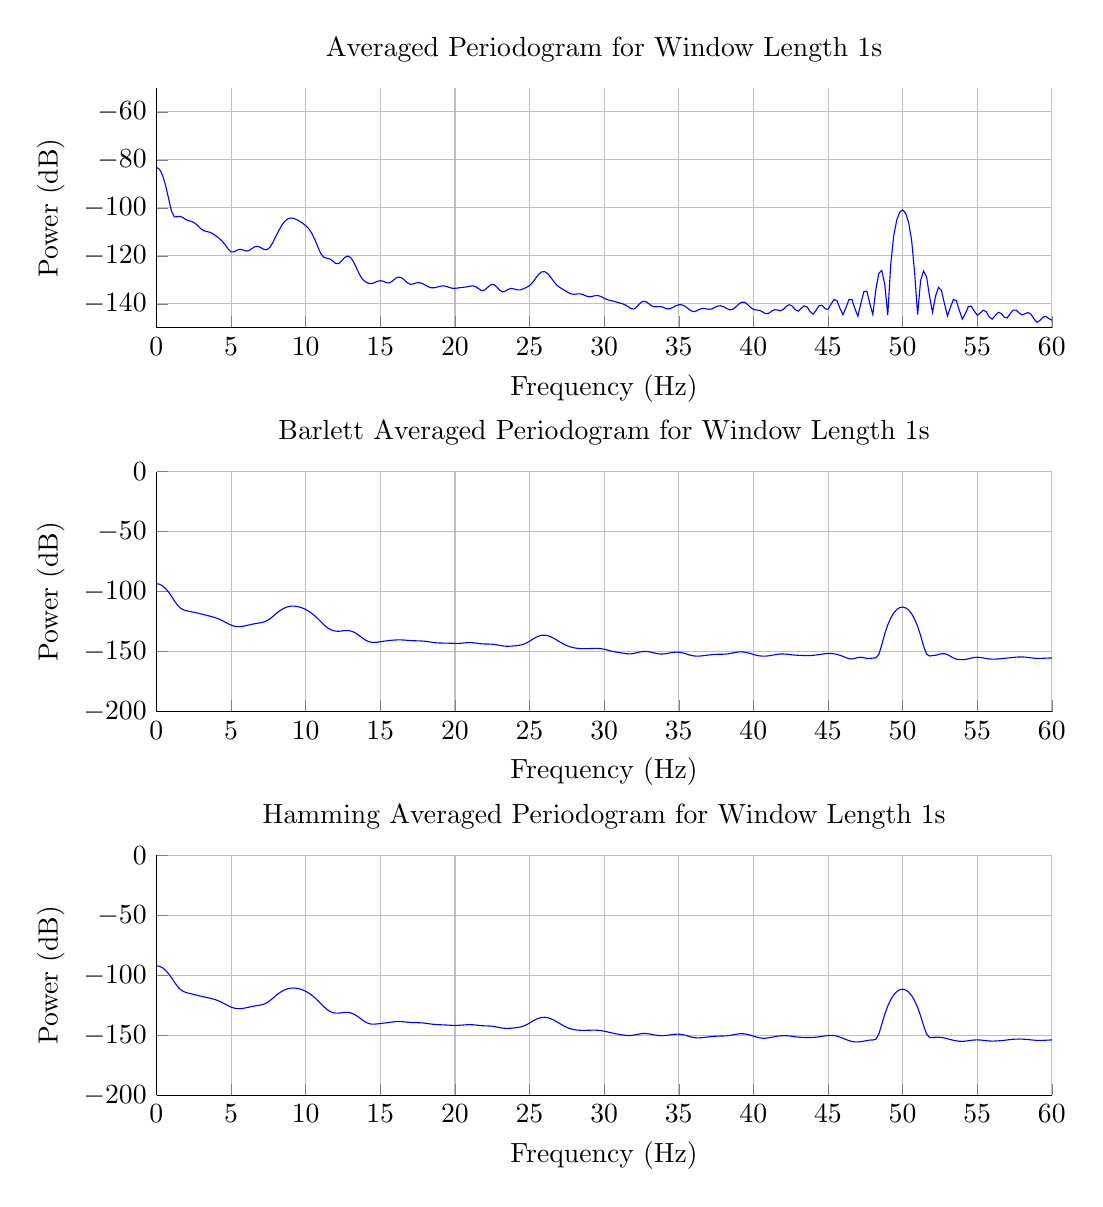
\begin{tikzpicture}

\begin{axis}[%
width=4.47708333333333in,
height=1.2in,
scale only axis,
xmin=0,
xmax=60,
xlabel={Frequency (Hz)},
xmajorgrids,
ymin=-200,
ymax=0,
ylabel={Power (dB)},
ymajorgrids,
name=plot2,
title={Barlett Averaged Periodogram for Window Length 1s},
axis x line*=bottom,
axis y line*=left
]
\addplot [color=blue,solid,forget plot]
  table[row sep=crcr]{-600	-178.672722947721\\
-599.8	-178.560050740982\\
-599.6	-178.284815501511\\
-599.4	-177.991082529571\\
-599.2	-177.816143667517\\
-599	-177.825777316799\\
-598.8	-177.991193335\\
-598.6	-178.20112944943\\
-598.4	-178.311523769513\\
-598.2	-178.22598785701\\
-598	-177.95573185528\\
-597.8	-177.601444411835\\
-597.6	-177.276583008711\\
-597.4	-177.043991985445\\
-597.2	-176.904751724336\\
-597	-176.831739728922\\
-596.8	-176.818169605555\\
-596.6	-176.903742382186\\
-596.4	-177.156725045404\\
-596.2	-177.624583142093\\
-596	-178.283978364118\\
-595.8	-179.017728239059\\
-595.6	-179.644915366867\\
-595.4	-180.012788257985\\
-595.2	-180.087751092074\\
-595	-179.945840400194\\
-594.8	-179.675310406283\\
-594.6	-179.306816525872\\
-594.4	-178.831349573584\\
-594.2	-178.266049421551\\
-594	-177.690466538345\\
-593.8	-177.218930466645\\
-593.6	-176.944012885966\\
-593.4	-176.899028964538\\
-593.2	-177.055331154075\\
-593	-177.347378941962\\
-592.8	-177.709809997863\\
-592.6	-178.102324109604\\
-592.4	-178.501455391807\\
-592.2	-178.866019147\\
-592	-179.11412695571\\
-591.8	-179.150512687117\\
-591.6	-178.93721365574\\
-591.4	-178.538444166565\\
-591.2	-178.084908138088\\
-591	-177.695476305398\\
-590.8	-177.427374832717\\
-590.6	-177.277283816038\\
-590.4	-177.213994182717\\
-590.2	-177.212344234196\\
-590	-177.263057248567\\
-589.8	-177.353176697357\\
-589.6	-177.437969894351\\
-589.4	-177.436552861101\\
-589.2	-177.269476017399\\
-589	-176.917591360715\\
-588.8	-176.44792027892\\
-588.6	-175.978750801666\\
-588.4	-175.618297503578\\
-588.2	-175.423381209699\\
-588	-175.390987357295\\
-587.8	-175.473419841011\\
-587.6	-175.605903135605\\
-587.4	-175.73526893801\\
-587.2	-175.835950000612\\
-587	-175.905201904261\\
-586.8	-175.944749094773\\
-586.6	-175.94616526998\\
-586.4	-175.892068861335\\
-586.2	-175.770737100197\\
-586	-175.590287624785\\
-585.8	-175.379460532496\\
-585.6	-175.17439155373\\
-585.4	-175.001723025819\\
-585.2	-174.868362607324\\
-585	-174.761559381027\\
-584.8	-174.657789582369\\
-584.6	-174.536739203778\\
-584.4	-174.395005231149\\
-584.2	-174.252848860026\\
-584	-174.149314227569\\
-583.8	-174.126996148822\\
-583.6	-174.213393236942\\
-583.4	-174.407197218697\\
-583.2	-174.676077135416\\
-583	-174.969311082632\\
-582.8	-175.242054167259\\
-582.6	-175.47787236275\\
-582.4	-175.692395770889\\
-582.2	-175.913835156834\\
-582	-176.155675441459\\
-581.8	-176.403340695651\\
-581.6	-176.626288557615\\
-581.4	-176.807499955138\\
-581.2	-176.964366926804\\
-581	-177.137339268466\\
-580.8	-177.350385909874\\
-580.6	-177.573217307961\\
-580.4	-177.718373688407\\
-580.2	-177.688395315283\\
-580	-177.446447348037\\
-579.8	-177.045861551952\\
-579.6	-176.589610459677\\
-579.4	-176.168363647697\\
-579.2	-175.834013104531\\
-579	-175.613639040274\\
-578.8	-175.533290418623\\
-578.6	-175.622314313162\\
-578.4	-175.892212688685\\
-578.2	-176.307722421131\\
-578	-176.777650074605\\
-577.8	-177.186301912193\\
-577.6	-177.455691133156\\
-577.4	-177.585474751796\\
-577.2	-177.627415881716\\
-577	-177.626399877381\\
-576.8	-177.595132838116\\
-576.6	-177.541012791033\\
-576.4	-177.501521376794\\
-576.2	-177.535696756836\\
-576	-177.669431831079\\
-575.8	-177.842375425145\\
-575.6	-177.91340879145\\
-575.4	-177.751432334951\\
-575.2	-177.350772445107\\
-575	-176.845313329807\\
-574.8	-176.404983051416\\
-574.6	-176.131716034802\\
-574.4	-176.029857987182\\
-574.2	-176.038114344729\\
-574	-176.08424148689\\
-573.8	-176.123753529852\\
-573.6	-176.138934476473\\
-573.4	-176.112891147318\\
-573.2	-176.019582420118\\
-573	-175.849916011213\\
-572.8	-175.646527130608\\
-572.6	-175.501784409118\\
-572.4	-175.510612872048\\
-572.2	-175.710956781244\\
-572	-176.045163005726\\
-571.8	-176.364543683117\\
-571.6	-176.497703192485\\
-571.4	-176.364782143745\\
-571.2	-176.041992936822\\
-571	-175.706016307353\\
-570.8	-175.524000998887\\
-570.6	-175.584305235601\\
-570.4	-175.882949307078\\
-570.2	-176.339939221161\\
-570	-176.829818481129\\
-569.8	-177.221383275703\\
-569.6	-177.416646622088\\
-569.4	-177.374306070481\\
-569.2	-177.112996308658\\
-569	-176.701566333393\\
-568.8	-176.241254799376\\
-568.6	-175.840204962761\\
-568.4	-175.585733443736\\
-568.2	-175.52360620854\\
-568	-175.649685866342\\
-567.8	-175.914383715881\\
-567.6	-176.238437744114\\
-567.4	-176.536461172873\\
-567.2	-176.740458857386\\
-567	-176.813705092104\\
-566.8	-176.750949543018\\
-566.6	-176.569501688449\\
-566.4	-176.299128105218\\
-566.2	-175.976537502054\\
-566	-175.646395858288\\
-565.8	-175.365877414545\\
-565.6	-175.204925234756\\
-565.4	-175.234301333174\\
-565.2	-175.499107223021\\
-565	-175.981984218091\\
-564.8	-176.568632236046\\
-564.6	-177.049194390991\\
-564.4	-177.206569293289\\
-564.2	-176.972574886269\\
-564	-176.493301526195\\
-563.8	-176.01530725233\\
-563.6	-175.730582239662\\
-563.4	-175.707164292535\\
-563.2	-175.895571235626\\
-563	-176.171148269502\\
-562.8	-176.395370515663\\
-562.6	-176.475714492038\\
-562.4	-176.390225417088\\
-562.2	-176.167752330126\\
-562	-175.856960411122\\
-561.8	-175.514391423848\\
-561.6	-175.205425772574\\
-561.4	-174.996671404776\\
-561.2	-174.934041940411\\
-561	-175.019203030034\\
-560.8	-175.20126696593\\
-560.6	-175.395298131643\\
-560.4	-175.525593029092\\
-560.2	-175.567930602208\\
-560	-175.55519701175\\
-559.8	-175.541912914752\\
-559.6	-175.562359748052\\
-559.4	-175.615906112969\\
-559.2	-175.683207528275\\
-559	-175.751640082402\\
-558.8	-175.823470789455\\
-558.6	-175.899887079677\\
-558.4	-175.962092880081\\
-558.2	-175.978505752641\\
-558	-175.943023726759\\
-557.8	-175.91081107292\\
-557.6	-175.989106057463\\
-557.4	-176.280260900658\\
-557.2	-176.81039930753\\
-557	-177.476124494549\\
-556.8	-178.047271621531\\
-556.6	-178.282418170536\\
-556.4	-178.123577514698\\
-556.2	-177.760418870621\\
-556	-177.475020830175\\
-555.8	-177.460249926616\\
-555.6	-177.745250592713\\
-555.4	-178.197931824861\\
-555.2	-178.576767221309\\
-555	-178.648067773073\\
-554.8	-178.327129771137\\
-554.6	-177.712554370972\\
-554.4	-176.982960519673\\
-554.2	-176.285224690154\\
-554	-175.699855053563\\
-553.8	-175.260663501207\\
-553.6	-174.983748544516\\
-553.4	-174.882396509362\\
-553.2	-174.963276391966\\
-553	-175.210110514067\\
-552.8	-175.567378848266\\
-552.6	-175.94032559162\\
-552.4	-176.223406856646\\
-552.2	-176.345041934526\\
-552	-176.284626704252\\
-551.8	-176.032828673194\\
-551.6	-175.53630101555\\
-551.4	-174.708086553515\\
-551.2	-173.525434585567\\
-551	-172.113861512034\\
-550.8	-170.709275744924\\
-550.6	-169.547166113929\\
-550.4	-168.789306799216\\
-550.2	-168.510813870554\\
-550	-168.713552985345\\
-549.8	-169.340293264115\\
-549.6	-170.283954197449\\
-549.4	-171.397952740341\\
-549.2	-172.518709763959\\
-549	-173.507063752289\\
-548.8	-174.295498790273\\
-548.6	-174.906882093848\\
-548.4	-175.422670295992\\
-548.2	-175.91979155932\\
-548	-176.415851123392\\
-547.8	-176.851768400601\\
-547.6	-177.126143666705\\
-547.4	-177.169783345474\\
-547.2	-177.002852090556\\
-547	-176.716813241545\\
-546.8	-176.403155550455\\
-546.6	-176.101374429952\\
-546.4	-175.802690165475\\
-546.2	-175.493775035648\\
-546	-175.19918826621\\
-545.8	-174.986665554162\\
-545.6	-174.933153219176\\
-545.4	-175.077900343916\\
-545.2	-175.387004728066\\
-545	-175.743839835069\\
-544.8	-175.98299250476\\
-544.6	-175.975866968667\\
-544.4	-175.71895822049\\
-544.2	-175.338759021909\\
-544	-175.009270082222\\
-543.8	-174.866451759027\\
-543.6	-174.9715781378\\
-543.4	-175.312239789656\\
-543.2	-175.816180750488\\
-543	-176.367036970389\\
-542.8	-176.825718436222\\
-542.6	-177.0685948963\\
-542.4	-177.041214927714\\
-542.2	-176.793173347591\\
-542	-176.454121195781\\
-541.8	-176.162426042184\\
-541.6	-175.997996756614\\
-541.4	-175.954011572518\\
-541.2	-175.955341032296\\
-541	-175.917829904955\\
-540.8	-175.816373331182\\
-540.6	-175.705056030033\\
-540.4	-175.667310740535\\
-540.2	-175.740258653101\\
-540	-175.871450886624\\
-539.8	-175.939658669335\\
-539.6	-175.839049841946\\
-539.4	-175.569211563628\\
-539.2	-175.242396954853\\
-539	-175.001611213984\\
-538.8	-174.932225632993\\
-538.6	-175.024505202677\\
-538.4	-175.189528630123\\
-538.2	-175.316020509672\\
-538	-175.343055812725\\
-537.8	-175.299729458201\\
-537.6	-175.279919344685\\
-537.4	-175.379293899367\\
-537.2	-175.64283699593\\
-537	-176.042119570255\\
-536.8	-176.480386261255\\
-536.6	-176.826831572145\\
-536.4	-176.978785320411\\
-536.2	-176.920619419049\\
-536	-176.729299190475\\
-535.8	-176.52036529295\\
-535.6	-176.383902992047\\
-535.4	-176.353703354586\\
-535.2	-176.414390641454\\
-535	-176.528501510883\\
-534.8	-176.658251799367\\
-534.6	-176.762614612017\\
-534.4	-176.776487292284\\
-534.2	-176.609866971958\\
-534	-176.200112842334\\
-533.8	-175.585811945218\\
-533.6	-174.917053221895\\
-533.4	-174.379648944229\\
-533.2	-174.103873342988\\
-533	-174.11489959752\\
-532.8	-174.329537624994\\
-532.6	-174.59647708731\\
-532.4	-174.77939134494\\
-532.2	-174.840996515804\\
-532	-174.852016172803\\
-531.8	-174.915283479011\\
-531.6	-175.081480435498\\
-531.4	-175.319191390009\\
-531.2	-175.545929931593\\
-531	-175.692947479887\\
-530.8	-175.754641576493\\
-530.6	-175.7817717128\\
-530.4	-175.830655389723\\
-530.2	-175.916828641808\\
-530	-176.004581449833\\
-529.8	-176.031951213208\\
-529.6	-175.951088355507\\
-529.4	-175.755712195235\\
-529.2	-175.478039211599\\
-529	-175.164329640223\\
-528.8	-174.853154517253\\
-528.6	-174.570607512814\\
-528.4	-174.338901259348\\
-528.2	-174.185531186547\\
-528	-174.142345803588\\
-527.8	-174.233065828371\\
-527.6	-174.45676285171\\
-527.4	-174.778615784017\\
-527.2	-175.137673400157\\
-527	-175.473169679565\\
-526.8	-175.754878094268\\
-526.6	-175.991923337219\\
-526.4	-176.209088442037\\
-526.2	-176.410491521\\
-526	-176.563288563034\\
-525.8	-176.618219915883\\
-525.6	-176.552583432406\\
-525.4	-176.396640078427\\
-525.2	-176.217275387906\\
-525	-176.075730866802\\
-524.8	-175.996116719318\\
-524.6	-175.963260426226\\
-524.4	-175.944255118833\\
-524.2	-175.915975104095\\
-524	-175.880851817448\\
-523.8	-175.864106633112\\
-523.6	-175.898569026873\\
-523.4	-176.005825815946\\
-523.2	-176.176730804911\\
-523	-176.353681564151\\
-522.8	-176.428578485893\\
-522.6	-176.281927601335\\
-522.4	-175.865035240208\\
-522.2	-175.262558264093\\
-522	-174.665060801571\\
-521.8	-174.27786749833\\
-521.6	-174.244369357574\\
-521.4	-174.60989757283\\
-521.2	-175.306744434229\\
-521	-176.151350149633\\
-520.8	-176.882922881427\\
-520.6	-177.280831038655\\
-520.4	-177.302608464893\\
-520.2	-177.09302350347\\
-520	-176.854025823229\\
-519.8	-176.725964417834\\
-519.6	-176.755769554817\\
-519.4	-176.918938789124\\
-519.2	-177.152748866702\\
-519	-177.383095941196\\
-518.8	-177.543714986861\\
-518.6	-177.592192262823\\
-518.4	-177.522920681765\\
-518.2	-177.36868774762\\
-518	-177.184073954099\\
-517.8	-177.017492190333\\
-517.6	-176.888087480446\\
-517.4	-176.779477053504\\
-517.2	-176.651880893498\\
-517	-176.465114817384\\
-516.8	-176.199665416379\\
-516.6	-175.865058035012\\
-516.4	-175.494016333601\\
-516.2	-175.129098003642\\
-516	-174.809132450366\\
-515.8	-174.559644048432\\
-515.6	-174.389945475359\\
-515.4	-174.29878090966\\
-515.2	-174.286454387062\\
-515	-174.36463368673\\
-514.8	-174.552198602212\\
-514.6	-174.852740345826\\
-514.4	-175.22371445381\\
-514.2	-175.561726432718\\
-514	-175.734899311564\\
-513.8	-175.666510728597\\
-513.6	-175.405210691341\\
-513.4	-175.101836981792\\
-513.2	-174.913561246346\\
-513	-174.922454168348\\
-512.8	-175.110498376465\\
-512.6	-175.386402717427\\
-512.4	-175.65005262381\\
-512.2	-175.860949512297\\
-512	-176.0554796473\\
-511.8	-176.294141002279\\
-511.6	-176.586912495947\\
-511.4	-176.860006554991\\
-511.2	-176.995982023799\\
-511	-176.927259178519\\
-510.8	-176.699113473221\\
-510.6	-176.432753083735\\
-510.4	-176.231301960315\\
-510.2	-176.118124479716\\
-510	-176.041489251622\\
-509.8	-175.927805352905\\
-509.6	-175.741035888077\\
-509.4	-175.501516432657\\
-509.2	-175.25497819285\\
-509	-175.031229114689\\
-508.8	-174.832579236124\\
-508.6	-174.654811691112\\
-508.4	-174.512923179586\\
-508.2	-174.442459996335\\
-508	-174.472299113762\\
-507.8	-174.589992508369\\
-507.6	-174.725977630792\\
-507.4	-174.774267599393\\
-507.2	-174.648157573036\\
-507	-174.336445822865\\
-506.8	-173.912200846196\\
-506.6	-173.489057519967\\
-506.4	-173.167836584073\\
-506.2	-173.007792594431\\
-506	-173.023582371629\\
-505.8	-173.195168122982\\
-505.6	-173.480775189538\\
-505.4	-173.82779375761\\
-505.2	-174.179374601398\\
-505	-174.47831595985\\
-504.8	-174.674852312948\\
-504.6	-174.744332030573\\
-504.4	-174.708471370714\\
-504.2	-174.640510673274\\
-504	-174.64122353973\\
-503.8	-174.79517241744\\
-503.6	-175.127244545303\\
-503.4	-175.57479963435\\
-503.2	-175.992385566796\\
-503	-176.212519850043\\
-502.8	-176.152220161726\\
-502.6	-175.878249205163\\
-502.4	-175.557694384134\\
-502.2	-175.349067252654\\
-502	-175.328922503959\\
-501.8	-175.477273617152\\
-501.6	-175.703238319486\\
-501.4	-175.896085898531\\
-501.2	-175.982500491543\\
-501	-175.954992062992\\
-500.8	-175.851037866604\\
-500.6	-175.707529262301\\
-500.4	-175.532873506891\\
-500.2	-175.314027849931\\
-500	-175.044036857102\\
-499.8	-174.742359746538\\
-499.6	-174.451185601934\\
-499.4	-174.214915426397\\
-499.2	-174.062330924722\\
-499	-174.002961826644\\
-498.8	-174.034638114081\\
-498.6	-174.151252260837\\
-498.4	-174.341620013813\\
-498.2	-174.579464516703\\
-498	-174.814485798743\\
-497.8	-174.97784038547\\
-497.6	-175.007105573419\\
-497.4	-174.877494009697\\
-497.2	-174.614732429857\\
-497	-174.279968546772\\
-496.8	-173.94337230886\\
-496.6	-173.667344948764\\
-496.4	-173.503220145432\\
-496.2	-173.492098717923\\
-496	-173.661357790387\\
-495.8	-174.01648701467\\
-495.6	-174.534288495122\\
-495.4	-175.164394836846\\
-495.2	-175.841061487278\\
-495	-176.49757605638\\
-494.8	-177.069535722693\\
-494.6	-177.484038440062\\
-494.4	-177.656556581307\\
-494.2	-177.523120311948\\
-494	-177.093694557707\\
-493.8	-176.466080035001\\
-493.6	-175.773505044082\\
-493.4	-175.115146357456\\
-493.2	-174.525511046051\\
-493	-173.992495130958\\
-492.8	-173.501542951741\\
-492.6	-173.072457393108\\
-492.4	-172.763411441547\\
-492.2	-172.643661871136\\
-492	-172.757604408539\\
-491.8	-173.099345669537\\
-491.6	-173.604059480411\\
-491.4	-174.158102220111\\
-491.2	-174.630819455615\\
-491	-174.922725337507\\
-490.8	-175.005798745566\\
-490.6	-174.927644820866\\
-490.4	-174.778682035704\\
-490.2	-174.648226901002\\
-490	-174.59173049662\\
-489.8	-174.615438362575\\
-489.6	-174.679329361306\\
-489.4	-174.720660249873\\
-489.2	-174.693512669456\\
-489	-174.601953936639\\
-488.8	-174.499491902541\\
-488.6	-174.453488963542\\
-488.4	-174.501677707898\\
-488.2	-174.627452104892\\
-488	-174.764690725633\\
-487.8	-174.831001030629\\
-487.6	-174.775357134444\\
-487.4	-174.611232310271\\
-487.2	-174.411820751945\\
-487	-174.274243259908\\
-486.8	-174.278726944972\\
-486.6	-174.459001796511\\
-486.4	-174.785871276317\\
-486.2	-175.166917689243\\
-486	-175.47470093732\\
-485.8	-175.608313833233\\
-485.6	-175.553236934856\\
-485.4	-175.380735286646\\
-485.2	-175.181781621933\\
-485	-174.996500079925\\
-484.8	-174.792916746002\\
-484.6	-174.505016059232\\
-484.4	-174.101769747376\\
-484.2	-173.630749097872\\
-484	-173.198031369316\\
-483.8	-172.908044273613\\
-483.6	-172.813364088316\\
-483.4	-172.89781240653\\
-483.2	-173.091523182276\\
-483	-173.310422150391\\
-482.8	-173.502627581534\\
-482.6	-173.67031522457\\
-482.4	-173.847585240574\\
-482.2	-174.053815502686\\
-482	-174.264368795038\\
-481.8	-174.426996408048\\
-481.6	-174.51628829824\\
-481.4	-174.577922483285\\
-481.2	-174.712998833552\\
-481	-175.007989202754\\
-480.8	-175.458177692901\\
-480.6	-175.928017314803\\
-480.4	-176.19106614055\\
-480.2	-176.075039345642\\
-480	-175.612109919832\\
-479.8	-175.020001871953\\
-479.6	-174.544951679596\\
-479.4	-174.343406236924\\
-479.2	-174.454681207487\\
-479	-174.815462558679\\
-478.8	-175.284016740457\\
-478.6	-175.68185271916\\
-478.4	-175.868041817999\\
-478.2	-175.817989897708\\
-478	-175.635554435909\\
-477.8	-175.478387697586\\
-477.6	-175.461471354443\\
-477.4	-175.599451814235\\
-477.2	-175.802169043676\\
-477	-175.925513626821\\
-476.8	-175.865541787036\\
-476.6	-175.630410055605\\
-476.4	-175.317809170982\\
-476.2	-175.024549891279\\
-476	-174.778671621615\\
-475.8	-174.539137213348\\
-475.6	-174.248429798697\\
-475.4	-173.891953012158\\
-475.2	-173.514756599844\\
-475	-173.186545947823\\
-474.8	-172.953524642928\\
-474.6	-172.816218132207\\
-474.4	-172.742797061294\\
-474.2	-172.703791504608\\
-474	-172.702091736412\\
-473.8	-172.775087789505\\
-473.6	-172.967090089712\\
-473.4	-173.291106076486\\
-473.2	-173.702132140452\\
-473	-174.098659683685\\
-472.8	-174.363241439032\\
-472.6	-174.430389877335\\
-472.4	-174.332058680344\\
-472.2	-174.176550879681\\
-472	-174.081843449294\\
-471.8	-174.118590537992\\
-471.6	-174.288677589691\\
-471.4	-174.534729539897\\
-471.2	-174.771173720731\\
-471	-174.92626272407\\
-470.8	-174.975097307403\\
-470.6	-174.943190418899\\
-470.4	-174.881802900909\\
-470.2	-174.837798677393\\
-470	-174.837671444979\\
-469.8	-174.887900650362\\
-469.6	-174.981956022138\\
-469.4	-175.103508735387\\
-469.2	-175.222703427037\\
-469	-175.292597426382\\
-468.8	-175.258260797504\\
-468.6	-175.083059023431\\
-468.4	-174.776354274164\\
-468.2	-174.396219833501\\
-468	-174.020423104766\\
-467.8	-173.707737581395\\
-467.6	-173.475287181975\\
-467.4	-173.301239817769\\
-467.2	-173.14725530317\\
-467	-172.98626705777\\
-466.8	-172.818443341719\\
-466.6	-172.66677362831\\
-466.4	-172.559384227659\\
-466.2	-172.51312632889\\
-466	-172.52748235765\\
-465.8	-172.589171551909\\
-465.6	-172.683480462488\\
-465.4	-172.807073177641\\
-465.2	-172.975772118374\\
-465	-173.220581683939\\
-464.8	-173.569367340047\\
-464.6	-174.019820554301\\
-464.4	-174.518251889471\\
-464.2	-174.965574533295\\
-464	-175.265798786938\\
-463.8	-175.394518295039\\
-463.6	-175.422514086582\\
-463.4	-175.461581933576\\
-463.2	-175.580798551708\\
-463	-175.759262084675\\
-462.8	-175.903307818325\\
-462.6	-175.919766730384\\
-462.4	-175.794064720861\\
-462.2	-175.601820583369\\
-462	-175.446558478161\\
-461.8	-175.389748424794\\
-461.6	-175.424906204645\\
-461.4	-175.496448972559\\
-461.2	-175.539059067457\\
-461	-175.510064636023\\
-460.8	-175.399007038034\\
-460.6	-175.220859433746\\
-460.4	-175.009257999215\\
-460.2	-174.813276005992\\
-460	-174.687876530569\\
-459.8	-174.672975595023\\
-459.6	-174.769754715315\\
-459.4	-174.92969994527\\
-459.2	-175.069270382163\\
-459	-175.110740732418\\
-458.8	-175.026555292627\\
-458.6	-174.852231626731\\
-458.4	-174.658978756839\\
-458.2	-174.514651632376\\
-458	-174.46264523329\\
-457.8	-174.522385182969\\
-457.6	-174.697268838216\\
-457.4	-174.975693698081\\
-457.2	-175.321014688317\\
-457	-175.659611258428\\
-456.8	-175.886660149933\\
-456.6	-175.906006867516\\
-456.4	-175.690040486998\\
-456.2	-175.308456966198\\
-456	-174.893194827922\\
-455.8	-174.570331325363\\
-455.6	-174.408202264743\\
-455.4	-174.398605594824\\
-455.2	-174.466603688743\\
-455	-174.506373958434\\
-454.8	-174.436724397287\\
-454.6	-174.247980984556\\
-454.4	-174.004662297185\\
-454.2	-173.804202624002\\
-454	-173.728228430586\\
-453.8	-173.814794716358\\
-453.6	-174.053495049963\\
-453.4	-174.394764885004\\
-453.2	-174.76820349672\\
-453	-175.107991390026\\
-452.8	-175.379048959555\\
-452.6	-175.58994563925\\
-452.4	-175.781083574231\\
-452.2	-175.9926984888\\
-452	-176.230789659251\\
-451.8	-176.448692322957\\
-451.6	-176.5540336963\\
-451.4	-176.441080156054\\
-451.2	-176.035389897786\\
-451	-175.328446507569\\
-450.8	-174.387026580484\\
-450.6	-173.337655155244\\
-450.4	-172.334868517634\\
-450.2	-171.524759038025\\
-450	-171.014963005583\\
-449.8	-170.856272255588\\
-449.6	-171.03490560787\\
-449.4	-171.475029450407\\
-449.2	-172.056025915693\\
-449	-172.647383538733\\
-448.8	-173.147423366638\\
-448.6	-173.497362403744\\
-448.4	-173.663440069448\\
-448.2	-173.621299377595\\
-448	-173.374481782818\\
-447.8	-172.985447320005\\
-447.6	-172.56954113766\\
-447.4	-172.245394435551\\
-447.2	-172.082570966838\\
-447	-172.07953528934\\
-446.8	-172.176987104667\\
-446.6	-172.296976130367\\
-446.4	-172.38720149753\\
-446.2	-172.441711042573\\
-446	-172.484887618155\\
-445.8	-172.538397589558\\
-445.6	-172.602744290938\\
-445.4	-172.666784075584\\
-445.2	-172.733102940956\\
-445	-172.834388651885\\
-444.8	-173.024607636553\\
-444.6	-173.350348579695\\
-444.4	-173.819993684086\\
-444.2	-174.385004065067\\
-444	-174.941784137892\\
-443.8	-175.360172202545\\
-443.6	-175.534635518416\\
-443.4	-175.432452743989\\
-443.2	-175.106232516543\\
-443	-174.666732392483\\
-442.8	-174.240821755552\\
-442.6	-173.93458098489\\
-442.4	-173.803904356809\\
-442.2	-173.830848652206\\
-442	-173.914645978984\\
-441.8	-173.902029134147\\
-441.6	-173.673063706717\\
-441.4	-173.233926410886\\
-441.2	-172.72155195056\\
-441	-172.311816478397\\
-440.8	-172.122513856458\\
-440.6	-172.170593363095\\
-440.4	-172.380338748378\\
-440.2	-172.629509695858\\
-440	-172.820308230873\\
-439.8	-172.936303340357\\
-439.6	-173.039323057796\\
-439.4	-173.212051296313\\
-439.2	-173.497483409768\\
-439	-173.869634113459\\
-438.8	-174.236209984848\\
-438.6	-174.464534857278\\
-438.4	-174.426036223814\\
-438.2	-174.050907294419\\
-438	-173.368603242141\\
-437.8	-172.504729304603\\
-437.6	-171.63404329308\\
-437.4	-170.922853671028\\
-437.2	-170.48962216169\\
-437	-170.386185032936\\
-436.8	-170.588979124137\\
-436.6	-170.996455088046\\
-436.4	-171.445962691587\\
-436.2	-171.772241295246\\
-436	-171.896840933438\\
-435.8	-171.875979775394\\
-435.6	-171.851632358532\\
-435.4	-171.953540254497\\
-435.2	-172.230672686361\\
-435	-172.636068670704\\
-434.8	-173.055696956974\\
-434.6	-173.368511903438\\
-434.4	-173.508395071517\\
-434.2	-173.484319031263\\
-434	-173.349510284398\\
-433.8	-173.160013566411\\
-433.6	-172.958340182334\\
-433.4	-172.778620598756\\
-433.2	-172.65207022864\\
-433	-172.603379462288\\
-432.8	-172.644740329008\\
-432.6	-172.775989521655\\
-432.4	-172.98894799555\\
-432.2	-173.26539143748\\
-432	-173.562573787282\\
-431.8	-173.797775644308\\
-431.6	-173.860203672749\\
-431.4	-173.668575397289\\
-431.2	-173.239854144198\\
-431	-172.697240440254\\
-430.8	-172.204121579654\\
-430.6	-171.887459670772\\
-430.4	-171.799353163519\\
-430.2	-171.915305331133\\
-430	-172.153649538002\\
-429.8	-172.409129348309\\
-429.6	-172.594488446974\\
-429.4	-172.672549539508\\
-429.2	-172.658244362304\\
-429	-172.590715357299\\
-428.8	-172.49908526973\\
-428.6	-172.385613725998\\
-428.4	-172.233306393714\\
-428.2	-172.028855088565\\
-428	-171.782824829994\\
-427.8	-171.532101381918\\
-427.6	-171.324557104277\\
-427.4	-171.198576918658\\
-427.2	-171.168944058203\\
-427	-171.221746960819\\
-426.8	-171.315980540721\\
-426.6	-171.391493085665\\
-426.4	-171.386613985856\\
-426.2	-171.26544679955\\
-426	-171.042093986393\\
-425.8	-170.782015978541\\
-425.6	-170.575505787364\\
-425.4	-170.500405647582\\
-425.2	-170.59459692457\\
-425	-170.846637851152\\
-424.8	-171.203337348302\\
-424.6	-171.589689742083\\
-424.4	-171.93333395278\\
-424.2	-172.182970876494\\
-424	-172.315244490768\\
-423.8	-172.335381187943\\
-423.6	-172.27861546203\\
-423.4	-172.208609046958\\
-423.2	-172.202947138249\\
-423	-172.324842890983\\
-422.8	-172.592283864005\\
-422.6	-172.9597189\\
-422.4	-173.326793014162\\
-422.2	-173.582057542629\\
-422	-173.662876466935\\
-421.8	-173.582495609242\\
-421.6	-173.398478638284\\
-421.4	-173.161063558704\\
-421.2	-172.895653695511\\
-421	-172.627884876834\\
-420.8	-172.414767848308\\
-420.6	-172.342950651596\\
-420.4	-172.490343377681\\
-420.2	-172.87700830578\\
-420	-173.432123903683\\
-419.8	-173.999488652381\\
-419.6	-174.401780388883\\
-419.4	-174.54176124543\\
-419.2	-174.449144850817\\
-419	-174.219102861546\\
-418.8	-173.918450662447\\
-418.6	-173.555536121329\\
-418.4	-173.121007607678\\
-418.2	-172.641507347605\\
-418	-172.190788418479\\
-417.8	-171.856005540342\\
-417.6	-171.698602625999\\
-417.4	-171.738689322284\\
-417.2	-171.961120187571\\
-417	-172.325702088424\\
-416.8	-172.766114217876\\
-416.6	-173.178312011855\\
-416.4	-173.42352993445\\
-416.2	-173.378766923731\\
-416	-173.020287963937\\
-415.8	-172.456840490359\\
-415.6	-171.866298015822\\
-415.4	-171.401183832864\\
-415.2	-171.138974615539\\
-415	-171.085304382549\\
-414.8	-171.2043850459\\
-414.6	-171.452239601892\\
-414.4	-171.794171187043\\
-414.2	-172.198652764046\\
-414	-172.619309702008\\
-413.8	-172.990721553356\\
-413.6	-173.254385300917\\
-413.4	-173.397011148648\\
-413.2	-173.457147561917\\
-413	-173.48172434689\\
-412.8	-173.468230586215\\
-412.6	-173.346974816328\\
-412.4	-173.031479844574\\
-412.2	-172.507073662273\\
-412	-171.873985919297\\
-411.8	-171.300468000151\\
-411.6	-170.939894091642\\
-411.4	-170.878210286113\\
-411.2	-171.1211455207\\
-411	-171.602700646832\\
-410.8	-172.204957063699\\
-410.6	-172.790218197103\\
-410.4	-173.242241625604\\
-410.2	-173.498481337448\\
-410	-173.554213137151\\
-409.8	-173.443137535422\\
-409.6	-173.217596473866\\
-409.4	-172.940880691942\\
-409.2	-172.684107283808\\
-409	-172.515946541062\\
-408.8	-172.482979316691\\
-408.6	-172.587313694315\\
-408.4	-172.772088970354\\
-408.2	-172.929508495163\\
-408	-172.945289470351\\
-407.8	-172.768098096295\\
-407.6	-172.451675687833\\
-407.4	-172.127756605854\\
-407.2	-171.936624756662\\
-407	-171.969796195971\\
-406.8	-172.242862231494\\
-406.6	-172.686661651151\\
-406.4	-173.150969293972\\
-406.2	-173.438133101874\\
-406	-173.387729749151\\
-405.8	-172.976442886578\\
-405.6	-172.336976093777\\
-405.4	-171.67047174171\\
-405.2	-171.141217955267\\
-405	-170.82411535821\\
-404.8	-170.702812778366\\
-404.6	-170.698546957526\\
-404.4	-170.719889577863\\
-404.2	-170.716727446771\\
-404	-170.705648723837\\
-403.8	-170.748175407123\\
-403.6	-170.903713122332\\
-403.4	-171.193559690765\\
-403.2	-171.591608246196\\
-403	-172.036055886253\\
-402.8	-172.450066458631\\
-402.6	-172.762776865011\\
-402.4	-172.92864061624\\
-402.2	-172.944100181983\\
-402	-172.852422787561\\
-401.8	-172.72544160399\\
-401.6	-172.627093260206\\
-401.4	-172.580650039201\\
-401.2	-172.560446088241\\
-401	-172.514136250459\\
-400.8	-172.401378104486\\
-400.6	-172.219002108924\\
-400.4	-171.992588639112\\
-400.2	-171.74824825352\\
-400	-171.496216942159\\
-399.8	-171.240078752375\\
-399.6	-170.996456170312\\
-399.4	-170.799855339825\\
-399.2	-170.68408185251\\
-399	-170.65562601869\\
-398.8	-170.6819264204\\
-398.6	-170.707140477635\\
-398.4	-170.688781110906\\
-398.2	-170.629033181751\\
-398	-170.574507002769\\
-397.8	-170.585834236688\\
-397.6	-170.702754939366\\
-397.4	-170.925586579236\\
-397.2	-171.216217871386\\
-397	-171.512039529573\\
-396.8	-171.745570145418\\
-396.6	-171.864716913098\\
-396.4	-171.849665522409\\
-396.2	-171.721099245888\\
-396	-171.534156546659\\
-395.8	-171.358024688378\\
-395.6	-171.249152991422\\
-395.4	-171.228722930124\\
-395.2	-171.27210423709\\
-395	-171.315520931287\\
-394.8	-171.282805930609\\
-394.6	-171.125289524227\\
-394.4	-170.851987251786\\
-394.2	-170.526941690955\\
-394	-170.236181143213\\
-393.8	-170.049019813142\\
-393.6	-169.993687435153\\
-393.4	-170.051754887357\\
-393.2	-170.168942298059\\
-393	-170.279174004087\\
-392.8	-170.334236827871\\
-392.6	-170.323788009032\\
-392.4	-170.272563134758\\
-392.2	-170.217942197675\\
-392	-170.185135561428\\
-391.8	-170.175473204967\\
-391.6	-170.172009430857\\
-391.4	-170.156284399011\\
-391.2	-170.124037873699\\
-391	-170.088549682268\\
-390.8	-170.069402034352\\
-390.6	-170.075146711439\\
-390.4	-170.091780408028\\
-390.2	-170.084602408232\\
-390	-170.013669468234\\
-389.8	-169.855551987792\\
-389.6	-169.61954744116\\
-389.4	-169.349609495219\\
-389.2	-169.112704938559\\
-389	-168.981126739303\\
-388.8	-169.015507697413\\
-388.6	-169.251260636402\\
-388.4	-169.689488985177\\
-388.2	-170.294979015234\\
-388	-171.005727645082\\
-387.8	-171.754972857195\\
-387.6	-172.494340040012\\
-387.4	-173.195776780909\\
-387.2	-173.821687255012\\
-387	-174.287986178479\\
-386.8	-174.472420377384\\
-386.6	-174.296399602681\\
-386.4	-173.815957515547\\
-386.2	-173.211584881182\\
-386	-172.682766869672\\
-385.8	-172.351873705413\\
-385.6	-172.227908368938\\
-385.4	-172.216654169034\\
-385.2	-172.166354549581\\
-385	-171.946538849607\\
-384.8	-171.525122604194\\
-384.6	-170.981807625975\\
-384.4	-170.448104185436\\
-384.2	-170.033190393549\\
-384	-169.784084816897\\
-383.8	-169.68374707171\\
-383.6	-169.675003189295\\
-383.4	-169.699346477556\\
-383.2	-169.732732405885\\
-383	-169.793504260199\\
-382.8	-169.912964210183\\
-382.6	-170.088724005098\\
-382.4	-170.255986001606\\
-382.2	-170.307011159213\\
-382	-170.162991125433\\
-381.8	-169.84774627248\\
-381.6	-169.488783515842\\
-381.4	-169.24397558365\\
-381.2	-169.222982577376\\
-381	-169.447451056145\\
-380.8	-169.847337719482\\
-380.6	-170.285858321911\\
-380.4	-170.615585345158\\
-380.2	-170.751513706892\\
-380	-170.712356212634\\
-379.8	-170.594446567705\\
-379.6	-170.506443871906\\
-379.4	-170.516586796329\\
-379.2	-170.631513201486\\
-379	-170.800720481536\\
-378.8	-170.942785070646\\
-378.6	-170.991352727921\\
-378.4	-170.941452945663\\
-378.2	-170.86048211431\\
-378	-170.850155608644\\
-377.8	-170.986309997407\\
-377.6	-171.271734494146\\
-377.4	-171.621481490176\\
-377.2	-171.894269170296\\
-377	-171.972371713755\\
-376.8	-171.843031785196\\
-376.6	-171.603547244225\\
-376.4	-171.384789253458\\
-376.2	-171.269203169469\\
-376	-171.25673048428\\
-375.8	-171.278096917168\\
-375.6	-171.238003788418\\
-375.4	-171.067505079929\\
-375.2	-170.757684522995\\
-375	-170.355561656246\\
-374.8	-169.931952900129\\
-374.6	-169.547451324765\\
-374.4	-169.233425039554\\
-374.2	-168.991051569551\\
-374	-168.805650750304\\
-373.8	-168.66935302565\\
-373.6	-168.598076750247\\
-373.4	-168.627605404039\\
-373.2	-168.786025783559\\
-373	-169.056986677644\\
-372.8	-169.358436018016\\
-372.6	-169.563914083461\\
-372.4	-169.575371726411\\
-372.2	-169.400457769534\\
-372	-169.15552842123\\
-371.8	-168.989455703999\\
-371.6	-169.003568181167\\
-371.4	-169.218783417791\\
-371.2	-169.585669981524\\
-371	-170.01497928662\\
-370.8	-170.406534295705\\
-370.6	-170.660729130446\\
-370.4	-170.681095885982\\
-370.2	-170.401138119932\\
-370	-169.842120726952\\
-369.8	-169.143308392199\\
-369.6	-168.514826086431\\
-369.4	-168.151157535097\\
-369.2	-168.166712987643\\
-369	-168.563155638963\\
-368.8	-169.211913638151\\
-368.6	-169.863313196853\\
-368.4	-170.235781177144\\
-368.2	-170.190189603689\\
-368	-169.829498680985\\
-367.8	-169.393258043234\\
-367.6	-169.082893168479\\
-367.4	-168.97898326713\\
-367.2	-169.04856197189\\
-367	-169.19108663215\\
-366.8	-169.297915090562\\
-366.6	-169.307226062983\\
-366.4	-169.229617263805\\
-366.2	-169.134811314593\\
-366	-169.11842553296\\
-365.8	-169.272304677059\\
-365.6	-169.663393477648\\
-365.4	-170.311771268025\\
-365.2	-171.158083979474\\
-365	-172.024648205203\\
-364.8	-172.614193519043\\
-364.6	-172.631577941143\\
-364.4	-172.007142744625\\
-364.2	-170.969982507814\\
-364	-169.866746975564\\
-363.8	-168.970639988388\\
-363.6	-168.429348697459\\
-363.4	-168.290615996654\\
-363.2	-168.534389780751\\
-363	-169.090574325587\\
-362.8	-169.844890012753\\
-362.6	-170.642177026029\\
-362.4	-171.301576854638\\
-362.2	-171.659332233208\\
-362	-171.634646724207\\
-361.8	-171.273568663194\\
-361.6	-170.724970367855\\
-361.4	-170.16679300424\\
-361.2	-169.739935562696\\
-361	-169.517049601201\\
-360.8	-169.4975676627\\
-360.6	-169.61599063599\\
-360.4	-169.762062231083\\
-360.2	-169.818408518691\\
-360	-169.711318116402\\
-359.8	-169.448206910169\\
-359.6	-169.112771105829\\
-359.4	-168.821764177744\\
-359.2	-168.675097132661\\
-359	-168.722408637786\\
-358.8	-168.949281381035\\
-358.6	-169.281360902724\\
-358.4	-169.610040168416\\
-358.2	-169.839941204107\\
-358	-169.936964359105\\
-357.8	-169.941491845653\\
-357.6	-169.937719434008\\
-357.4	-170.008561352024\\
-357.2	-170.205024523455\\
-357	-170.532624510985\\
-356.8	-170.944677376422\\
-356.6	-171.341343656945\\
-356.4	-171.590123018551\\
-356.2	-171.582813915162\\
-356	-171.30317054977\\
-355.8	-170.840478027647\\
-355.6	-170.329476998479\\
-355.4	-169.875455758821\\
-355.2	-169.521009040809\\
-355	-169.259637234981\\
-354.8	-169.072387615751\\
-354.6	-168.95837143125\\
-354.4	-168.938024084076\\
-354.2	-169.02941086388\\
-354	-169.218168273605\\
-353.8	-169.445447652491\\
-353.6	-169.628180573538\\
-353.4	-169.705321417461\\
-353.2	-169.676683700277\\
-353	-169.598199759183\\
-352.8	-169.536880589239\\
-352.6	-169.523931790965\\
-352.4	-169.537573225734\\
-352.2	-169.522760053824\\
-352	-169.435110133488\\
-351.8	-169.278571188744\\
-351.6	-169.104876693059\\
-351.4	-168.972672907714\\
-351.2	-168.896414107492\\
-351	-168.819498845668\\
-350.8	-168.63569321211\\
-350.6	-168.262112493644\\
-350.4	-167.7178350828\\
-350.2	-167.133305142555\\
-350	-166.681436280545\\
-349.8	-166.497333976331\\
-349.6	-166.634181934755\\
-349.4	-167.052695273787\\
-349.2	-167.633007754332\\
-349	-168.213777076419\\
-348.8	-168.660920355743\\
-348.6	-168.931059921571\\
-348.4	-169.074374100913\\
-348.2	-169.175437939268\\
-348	-169.289738196297\\
-347.8	-169.418307038122\\
-347.6	-169.520195706292\\
-347.4	-169.545474661911\\
-347.2	-169.471084955602\\
-347	-169.322623178419\\
-346.8	-169.170475224628\\
-346.6	-169.102304250056\\
-346.4	-169.185570546698\\
-346.2	-169.434235058896\\
-346	-169.790096453286\\
-345.8	-170.132163590867\\
-345.6	-170.328543620426\\
-345.4	-170.316030102109\\
-345.2	-170.143813995807\\
-345	-169.934813339169\\
-344.8	-169.803506642674\\
-344.6	-169.79723413526\\
-344.4	-169.883730154535\\
-344.2	-169.97598401308\\
-344	-169.979961182666\\
-343.8	-169.840991786004\\
-343.6	-169.557428957003\\
-343.4	-169.154700443664\\
-343.2	-168.651518994641\\
-343	-168.054781903909\\
-342.8	-167.387486540938\\
-342.6	-166.719738945534\\
-342.4	-166.169710042556\\
-342.2	-165.872209272435\\
-342	-165.938250434375\\
-341.8	-166.422546479364\\
-341.6	-167.297738000876\\
-341.4	-168.431709555694\\
-341.2	-169.586399468081\\
-341	-170.486703070925\\
-340.8	-170.969602546969\\
-340.6	-171.083361440728\\
-340.4	-171.00935257944\\
-340.2	-170.907117797603\\
-340	-170.838806665206\\
-339.8	-170.786172039728\\
-339.6	-170.70161036631\\
-339.4	-170.547423067511\\
-339.2	-170.306833566133\\
-339	-169.977599611026\\
-338.8	-169.568317679586\\
-338.6	-169.10361578374\\
-338.4	-168.628302588359\\
-338.2	-168.201165834381\\
-338	-167.880806637549\\
-337.8	-167.711822549967\\
-337.6	-167.715696855079\\
-337.4	-167.885401533595\\
-337.2	-168.182437339412\\
-337	-168.539137922014\\
-336.8	-168.87238164627\\
-336.6	-169.110125232608\\
-336.4	-169.217626366283\\
-336.2	-169.201518823887\\
-336	-169.08625055156\\
-335.8	-168.885016518044\\
-335.6	-168.593091979608\\
-335.4	-168.210253140873\\
-335.2	-167.771690261639\\
-335	-167.358070105246\\
-334.8	-167.075552564568\\
-334.6	-167.022062233059\\
-334.4	-167.258001145402\\
-334.2	-167.784861133126\\
-334	-168.527399152903\\
-333.8	-169.324946152823\\
-333.6	-169.960781371663\\
-333.4	-170.259272325918\\
-333.2	-170.20158626171\\
-333	-169.934103830253\\
-332.8	-169.650397915039\\
-332.6	-169.469524580866\\
-332.4	-169.39234331448\\
-332.2	-169.332447638068\\
-332	-169.196420503669\\
-331.8	-168.965985856547\\
-331.6	-168.713790162365\\
-331.4	-168.5377924502\\
-331.2	-168.475992121457\\
-331	-168.465124548266\\
-330.8	-168.370913143764\\
-330.6	-168.083689850562\\
-330.4	-167.612167702064\\
-330.2	-167.082921231643\\
-330	-166.652462825806\\
-329.8	-166.42537177103\\
-329.6	-166.429426322426\\
-329.4	-166.635078730995\\
-329.2	-166.991694483574\\
-329	-167.456140755745\\
-328.8	-167.994104736973\\
-328.6	-168.551329014003\\
-328.4	-169.019813788873\\
-328.2	-169.24576713437\\
-328	-169.111077457811\\
-327.8	-168.636662446855\\
-327.6	-167.991725343904\\
-327.4	-167.393219203233\\
-327.2	-167.000476446639\\
-327	-166.86907559621\\
-326.8	-166.951563116335\\
-326.6	-167.127220781387\\
-326.4	-167.261099831352\\
-326.2	-167.277118004781\\
-326	-167.193306826093\\
-325.8	-167.084625675659\\
-325.6	-167.011593390958\\
-325.4	-166.979551263657\\
-325.2	-166.953932745066\\
-325	-166.91045948905\\
-324.8	-166.872565220498\\
-324.6	-166.899574856542\\
-324.4	-167.037068762431\\
-324.2	-167.273102209294\\
-324	-167.534485339113\\
-323.8	-167.730181836249\\
-323.6	-167.813897813005\\
-323.4	-167.811487872466\\
-323.2	-167.788278245587\\
-323	-167.795124345646\\
-322.8	-167.844726607648\\
-322.6	-167.928738417407\\
-322.4	-168.048479085686\\
-322.2	-168.225436837984\\
-322	-168.481714342967\\
-321.8	-168.810852505547\\
-321.6	-169.166956870966\\
-321.4	-169.483242687001\\
-321.2	-169.705203969066\\
-321	-169.808139597157\\
-320.8	-169.785446196234\\
-320.6	-169.630178366415\\
-320.4	-169.340220460798\\
-320.2	-168.944051360462\\
-320	-168.513158286276\\
-319.8	-168.140717540672\\
-319.6	-167.904063105954\\
-319.4	-167.839994793125\\
-319.2	-167.944106345747\\
-319	-168.186954445735\\
-318.8	-168.531841398069\\
-318.6	-168.939779925117\\
-318.4	-169.358522156732\\
-318.2	-169.710887373412\\
-318	-169.907400948336\\
-317.8	-169.890331762358\\
-317.6	-169.674244480147\\
-317.4	-169.335667046219\\
-317.2	-168.956714244703\\
-317	-168.575997170266\\
-316.8	-168.185607317159\\
-316.6	-167.770455114928\\
-316.4	-167.354184152874\\
-316.2	-167.010698070003\\
-316	-166.831597525408\\
-315.8	-166.875643321359\\
-315.6	-167.128904394168\\
-315.4	-167.490752033183\\
-315.2	-167.800711537367\\
-315	-167.916720416737\\
-314.8	-167.806687892806\\
-314.6	-167.568500073942\\
-314.4	-167.35623986008\\
-314.2	-167.287675570017\\
-314	-167.395753569389\\
-313.8	-167.626791407599\\
-313.6	-167.871556664677\\
-313.4	-168.020396684333\\
-313.2	-168.020189848494\\
-313	-167.894829864948\\
-312.8	-167.715662151302\\
-312.6	-167.55380518555\\
-312.4	-167.451643372953\\
-312.2	-167.420883643969\\
-312	-167.452927071511\\
-311.8	-167.526823648007\\
-311.6	-167.611371812921\\
-311.4	-167.669473568081\\
-311.2	-167.673664902334\\
-311	-167.627731970755\\
-310.8	-167.574037135463\\
-310.6	-167.571971639203\\
-310.4	-167.657400541964\\
-310.2	-167.808889780438\\
-310	-167.944794422326\\
-309.8	-167.963610841671\\
-309.6	-167.810935212544\\
-309.4	-167.519459747124\\
-309.2	-167.183076961796\\
-309	-166.894288230407\\
-308.8	-166.701370459597\\
-308.6	-166.606487617552\\
-308.4	-166.590319353366\\
-308.2	-166.638086637623\\
-308	-166.74806161217\\
-307.8	-166.920761046617\\
-307.6	-167.143265942906\\
-307.4	-167.384372193625\\
-307.2	-167.603098482646\\
-307	-167.75914736229\\
-306.8	-167.814336129677\\
-306.6	-167.73099397543\\
-306.4	-167.485495626911\\
-306.2	-167.098106279972\\
-306	-166.648919112505\\
-305.8	-166.252681614358\\
-305.6	-166.006226937835\\
-305.4	-165.944850047926\\
-305.2	-166.031398860884\\
-305	-166.185241047535\\
-304.8	-166.341518834362\\
-304.6	-166.501368392401\\
-304.4	-166.724080250302\\
-304.2	-167.058996059327\\
-304	-167.468089547935\\
-303.8	-167.800996373072\\
-303.6	-167.872292561758\\
-303.4	-167.618468485467\\
-303.2	-167.178528369617\\
-303	-166.795394560708\\
-302.8	-166.659144210926\\
-302.6	-166.824254158951\\
-302.4	-167.20429135824\\
-302.2	-167.620081837802\\
-302	-167.899117133073\\
-301.8	-167.982346012402\\
-301.6	-167.941206722145\\
-301.4	-167.886411445871\\
-301.2	-167.867260630621\\
-301	-167.841898311569\\
-300.8	-167.722558311377\\
-300.6	-167.455427586973\\
-300.4	-167.072193563289\\
-300.2	-166.674441699539\\
-300	-166.378036886672\\
-299.8	-166.26736440605\\
-299.6	-166.374581190506\\
-299.4	-166.670845785344\\
-299.2	-167.060488261045\\
-299	-167.390702562526\\
-298.8	-167.504300450626\\
-298.6	-167.332319552954\\
-298.4	-166.951333049375\\
-298.2	-166.537855004957\\
-298	-166.265806524118\\
-297.8	-166.232856091135\\
-297.6	-166.437296110966\\
-297.4	-166.786545353065\\
-297.2	-167.128103965774\\
-297	-167.306296628606\\
-296.8	-167.232127978492\\
-296.6	-166.924456746343\\
-296.4	-166.492084812113\\
-296.2	-166.07756651211\\
-296	-165.803558391761\\
-295.8	-165.737827518885\\
-295.6	-165.872269546748\\
-295.4	-166.115780882758\\
-295.2	-166.318809032121\\
-295	-166.349286087572\\
-294.8	-166.188544267581\\
-294.6	-165.957636416257\\
-294.4	-165.841332169886\\
-294.2	-165.983525766851\\
-294	-166.419087616593\\
-293.8	-167.043968829946\\
-293.6	-167.624180865526\\
-293.4	-167.884876864626\\
-293.2	-167.6834899313\\
-293	-167.116885510042\\
-292.8	-166.43137925414\\
-292.6	-165.857938584871\\
-292.4	-165.529901645285\\
-292.2	-165.481560747908\\
-292	-165.670904454489\\
-291.8	-166.001554354112\\
-291.6	-166.347242231313\\
-291.4	-166.587275397747\\
-291.2	-166.646369997979\\
-291	-166.514238191686\\
-290.8	-166.229980786749\\
-290.6	-165.849478978493\\
-290.4	-165.425753954068\\
-290.2	-165.010383153397\\
-290	-164.660784329646\\
-289.8	-164.436421037352\\
-289.6	-164.381088988369\\
-289.4	-164.50114720597\\
-289.2	-164.753047488246\\
-289	-165.051873015336\\
-288.8	-165.30552191032\\
-288.6	-165.459087893\\
-288.4	-165.513565292688\\
-288.2	-165.498697201192\\
-288	-165.42594841335\\
-287.8	-165.267902265416\\
-287.6	-164.985583275231\\
-287.4	-164.58126844929\\
-287.2	-164.126535714588\\
-287	-163.738980994892\\
-286.8	-163.532815680687\\
-286.6	-163.581176600561\\
-286.4	-163.900949339713\\
-286.2	-164.450647526292\\
-286	-165.133164957835\\
-285.8	-165.807317807374\\
-285.6	-166.321934285113\\
-285.4	-166.575109291041\\
-285.2	-166.563336100486\\
-285	-166.371670564674\\
-284.8	-166.110886581687\\
-284.6	-165.859152746103\\
-284.4	-165.647124243509\\
-284.2	-165.480931272353\\
-284	-165.373714380872\\
-283.8	-165.3561979354\\
-283.6	-165.456678643402\\
-283.4	-165.666659224579\\
-283.2	-165.920510763445\\
-283	-166.113390798532\\
-282.8	-166.159895084101\\
-282.6	-166.053259531703\\
-282.4	-165.866572513978\\
-282.2	-165.692358820806\\
-282	-165.577223989466\\
-281.8	-165.498391838376\\
-281.6	-165.390088791231\\
-281.4	-165.201309696714\\
-281.2	-164.945227079298\\
-281	-164.700649163105\\
-280.8	-164.56622869883\\
-280.6	-164.603956592564\\
-280.4	-164.801606191714\\
-280.2	-165.065640315025\\
-280	-165.255435127346\\
-279.8	-165.261244356682\\
-279.6	-165.081250548377\\
-279.4	-164.82464004038\\
-279.2	-164.63663756077\\
-279	-164.61702169364\\
-278.8	-164.781887141095\\
-278.6	-165.068532067597\\
-278.4	-165.370399341965\\
-278.2	-165.588317762456\\
-278	-165.672209663581\\
-277.8	-165.626659562852\\
-277.6	-165.484956343927\\
-277.4	-165.283733238851\\
-277.2	-165.057852055614\\
-277	-164.845791107495\\
-276.8	-164.686416803043\\
-276.6	-164.602231299635\\
-276.4	-164.581695427613\\
-276.2	-164.57852217397\\
-276	-164.537209542496\\
-275.8	-164.433431179144\\
-275.6	-164.297642439072\\
-275.4	-164.198466682654\\
-275.2	-164.198262573485\\
-275	-164.313710838291\\
-274.8	-164.503757919993\\
-274.6	-164.690095505695\\
-274.4	-164.800913740719\\
-274.2	-164.811660076385\\
-274	-164.753437067998\\
-273.8	-164.687401258064\\
-273.6	-164.672056813854\\
-273.4	-164.744914269383\\
-273.2	-164.916880577153\\
-273	-165.167524972086\\
-272.8	-165.437851032942\\
-272.6	-165.63378362156\\
-272.4	-165.660742584081\\
-272.2	-165.485790801601\\
-272	-165.178703308083\\
-271.8	-164.885951482997\\
-271.6	-164.758238814463\\
-271.4	-164.885028017377\\
-271.2	-165.257197801863\\
-271	-165.753923866234\\
-270.8	-166.166347116606\\
-270.6	-166.289076234214\\
-270.4	-166.053540906225\\
-270.2	-165.577043786839\\
-270	-165.066175548385\\
-269.8	-164.684165833244\\
-269.6	-164.485725328385\\
-269.4	-164.421294784231\\
-269.2	-164.385361137107\\
-269	-164.289987618564\\
-268.8	-164.124452231324\\
-268.6	-163.95317782877\\
-268.4	-163.855273119938\\
-268.2	-163.860513345511\\
-268	-163.927001979804\\
-267.8	-163.971442040072\\
-267.6	-163.93332541161\\
-267.4	-163.824698529261\\
-267.2	-163.721310284288\\
-267	-163.70758427854\\
-266.8	-163.826559414451\\
-266.6	-164.065294724226\\
-266.4	-164.371838792957\\
-266.2	-164.683785217268\\
-266	-164.947598930275\\
-265.8	-165.121704180278\\
-265.6	-165.177175057536\\
-265.4	-165.111784192156\\
-265.2	-164.967631073367\\
-265	-164.824512912431\\
-264.8	-164.762019389022\\
-264.6	-164.815827659951\\
-264.4	-164.958671535561\\
-264.2	-165.120286570596\\
-264	-165.237577252414\\
-263.8	-165.298393416321\\
-263.6	-165.338294991614\\
-263.4	-165.393574812798\\
-263.2	-165.457298536903\\
-263	-165.478266348568\\
-262.8	-165.403184952442\\
-262.6	-165.222761435215\\
-262.4	-164.976267089435\\
-262.2	-164.714379329632\\
-262	-164.464306736188\\
-261.8	-164.230709408058\\
-261.6	-164.024552823806\\
-261.4	-163.885305703994\\
-261.2	-163.870452112387\\
-261	-164.018361938359\\
-260.8	-164.311750369183\\
-260.6	-164.667904553431\\
-260.4	-164.972254550268\\
-260.2	-165.14789147772\\
-260	-165.210085922428\\
-259.8	-165.249121911738\\
-259.6	-165.352656792274\\
-259.4	-165.530521812124\\
-259.2	-165.688718826803\\
-259	-165.674731070401\\
-258.8	-165.387078511488\\
-258.6	-164.868701481539\\
-258.4	-164.286091840352\\
-258.2	-163.820792858217\\
-258	-163.578598283787\\
-257.8	-163.559294885481\\
-257.6	-163.67336954139\\
-257.4	-163.794214457347\\
-257.2	-163.832379973796\\
-257	-163.787806903845\\
-256.8	-163.735225995462\\
-256.6	-163.759254156416\\
-256.4	-163.897347557896\\
-256.2	-164.12417948075\\
-256	-164.374101100425\\
-255.8	-164.58058585356\\
-255.6	-164.705237037036\\
-255.4	-164.739266844221\\
-255.2	-164.687801054438\\
-255	-164.562222853664\\
-254.8	-164.389437261622\\
-254.6	-164.222165032493\\
-254.4	-164.131695336707\\
-254.2	-164.183131024167\\
-254	-164.40702555515\\
-253.8	-164.778659932939\\
-253.6	-165.210273807584\\
-253.4	-165.56418225592\\
-253.2	-165.697557955347\\
-253	-165.52978337291\\
-252.8	-165.085509229498\\
-252.6	-164.473073351153\\
-252.4	-163.82290517677\\
-252.2	-163.241340406135\\
-252	-162.799396119864\\
-251.8	-162.537539494392\\
-251.6	-162.459653984952\\
-251.4	-162.502284164994\\
-251.2	-162.493740879582\\
-251	-162.167783361219\\
-250.8	-161.315189773935\\
-250.6	-159.990443614401\\
-250.4	-158.510077183523\\
-250.2	-157.242998310848\\
-250	-156.452430815311\\
-249.8	-156.267375606172\\
-249.6	-156.701636455298\\
-249.4	-157.66126909993\\
-249.2	-158.935921900627\\
-249	-160.215212146965\\
-248.8	-161.196621405287\\
-248.6	-161.759968963821\\
-248.4	-162.019687710089\\
-248.2	-162.179714319214\\
-248	-162.374930617317\\
-247.8	-162.629322521053\\
-247.6	-162.896538438848\\
-247.4	-163.117339642239\\
-247.2	-163.257972925779\\
-247	-163.32201441459\\
-246.8	-163.345687071129\\
-246.6	-163.385356687697\\
-246.4	-163.496779342372\\
-246.2	-163.706941632164\\
-246	-163.989370004801\\
-245.8	-164.261452823201\\
-245.6	-164.419767678834\\
-245.4	-164.404464243769\\
-245.2	-164.244483668108\\
-245	-164.040214454848\\
-244.8	-163.903475081649\\
-244.6	-163.908004913104\\
-244.4	-164.073246033854\\
-244.2	-164.370629452239\\
-244	-164.736220142123\\
-243.8	-165.083483671509\\
-243.6	-165.320797493922\\
-243.4	-165.379627884977\\
-243.2	-165.244281347636\\
-243	-164.958507339677\\
-242.8	-164.597748924867\\
-242.6	-164.22864921969\\
-242.4	-163.886742109556\\
-242.2	-163.582979581596\\
-242	-163.326380284646\\
-241.8	-163.140108592147\\
-241.6	-163.056003883478\\
-241.4	-163.091774624683\\
-241.2	-163.228997476403\\
-241	-163.409702715686\\
-240.8	-163.558257272053\\
-240.6	-163.616616472013\\
-240.4	-163.56514297108\\
-240.2	-163.412036597812\\
-240	-163.169198718562\\
-239.8	-162.847178047525\\
-239.6	-162.475787004911\\
-239.4	-162.12230246929\\
-239.2	-161.878184277597\\
-239	-161.817312269103\\
-238.8	-161.952248681542\\
-238.6	-162.213892827345\\
-238.4	-162.4750836317\\
-238.2	-162.626320551945\\
-238	-162.661927682763\\
-237.8	-162.693922155938\\
-237.6	-162.873889861137\\
-237.4	-163.292901790826\\
-237.2	-163.918148711535\\
-237	-164.58139922928\\
-236.8	-165.040293473573\\
-236.6	-165.120442550627\\
-236.4	-164.836383868458\\
-236.2	-164.356913126545\\
-236	-163.869590885409\\
-235.8	-163.49417336947\\
-235.6	-163.277907719721\\
-235.4	-163.223352496853\\
-235.2	-163.310612100803\\
-235	-163.506012640033\\
-234.8	-163.765764287352\\
-234.6	-164.043280248727\\
-234.4	-164.29789251683\\
-234.2	-164.494783591803\\
-234	-164.595026656319\\
-233.8	-164.553952636834\\
-233.6	-164.346965438693\\
-233.4	-164.008871618956\\
-233.2	-163.641986815148\\
-233	-163.372509385924\\
-232.8	-163.285129638699\\
-232.6	-163.374365660614\\
-232.4	-163.531662383344\\
-232.2	-163.583786207573\\
-232	-163.388206949957\\
-231.8	-162.930338149881\\
-231.6	-162.329161185989\\
-231.4	-161.750556633714\\
-231.2	-161.321401261639\\
-231	-161.097409821137\\
-230.8	-161.070452875671\\
-230.6	-161.189752539781\\
-230.4	-161.385464959265\\
-230.2	-161.591581645856\\
-230	-161.764680044166\\
-229.8	-161.893023247214\\
-229.6	-161.993307001183\\
-229.4	-162.09890740551\\
-229.2	-162.246667607168\\
-229	-162.465965825497\\
-228.8	-162.76861121126\\
-228.6	-163.136879666333\\
-228.4	-163.512015361037\\
-228.2	-163.795335840864\\
-228	-163.879933438013\\
-227.8	-163.712906831369\\
-227.6	-163.344876561234\\
-227.4	-162.915491047446\\
-227.2	-162.585306996299\\
-227	-162.469022306394\\
-226.8	-162.599606390553\\
-226.6	-162.919699369904\\
-226.4	-163.297467601601\\
-226.2	-163.576183218377\\
-226	-163.650459570159\\
-225.8	-163.517275646838\\
-225.6	-163.252903377313\\
-225.4	-162.944038410607\\
-225.2	-162.641536738614\\
-225	-162.363034624769\\
-224.8	-162.121786887402\\
-224.6	-161.94620344869\\
-224.4	-161.871228279064\\
-224.2	-161.909851218016\\
-224	-162.028752040699\\
-223.8	-162.150903298333\\
-223.6	-162.195044039774\\
-223.4	-162.133428961407\\
-223.2	-162.0202743384\\
-223	-161.961037473216\\
-222.8	-162.047952989264\\
-222.6	-162.306635854115\\
-222.4	-162.675768263811\\
-222.2	-163.027090876287\\
-222	-163.228184119686\\
-221.8	-163.219969486932\\
-221.6	-163.044922215223\\
-221.4	-162.799664755056\\
-221.2	-162.565396657346\\
-221	-162.37625865825\\
-220.8	-162.233186463068\\
-220.6	-162.135372733103\\
-220.4	-162.098597655599\\
-220.2	-162.147964208099\\
-220	-162.296570663363\\
-219.8	-162.531560976689\\
-219.6	-162.819988264967\\
-219.4	-163.129396618562\\
-219.2	-163.443915179913\\
-219	-163.758490395606\\
-218.8	-164.054776649975\\
-218.6	-164.28371710542\\
-218.4	-164.380163683447\\
-218.2	-164.307956459224\\
-218	-164.096704137374\\
-217.8	-163.830149881983\\
-217.6	-163.594726715976\\
-217.4	-163.432124938991\\
-217.2	-163.325116648051\\
-217	-163.218551433471\\
-216.8	-163.061151854544\\
-216.6	-162.842502570823\\
-216.4	-162.601040189334\\
-216.2	-162.402608313791\\
-216	-162.311985175304\\
-215.8	-162.376256124064\\
-215.6	-162.620176029095\\
-215.4	-163.041761131994\\
-215.2	-163.597229400034\\
-215	-164.176331493174\\
-214.8	-164.59303305909\\
-214.6	-164.640373488676\\
-214.4	-164.220166751041\\
-214.2	-163.434409536524\\
-214	-162.521678848251\\
-213.8	-161.715033668777\\
-213.6	-161.156223149571\\
-213.4	-160.882993513973\\
-213.2	-160.846036812455\\
-213	-160.931699662204\\
-212.8	-160.99336098594\\
-212.6	-160.90090802477\\
-212.4	-160.598583554144\\
-212.2	-160.134361665481\\
-212	-159.634339233049\\
-211.8	-159.242784912568\\
-211.6	-159.068400759876\\
-211.4	-159.154535346012\\
-211.2	-159.470243194786\\
-211	-159.921046953756\\
-210.8	-160.386734963419\\
-210.6	-160.78206743067\\
-210.4	-161.101558758227\\
-210.2	-161.402792252766\\
-210	-161.737274355188\\
-209.8	-162.085856714916\\
-209.6	-162.347289336158\\
-209.4	-162.395574661438\\
-209.2	-162.172016651377\\
-209	-161.728661679258\\
-208.8	-161.181674442779\\
-208.6	-160.635275381703\\
-208.4	-160.147833746534\\
-208.2	-159.746370749824\\
-208	-159.456628120058\\
-207.8	-159.318759481377\\
-207.6	-159.378874149419\\
-207.4	-159.66463041572\\
-207.2	-160.158073439308\\
-207	-160.776482159272\\
-206.8	-161.37520896919\\
-206.6	-161.792361165181\\
-206.4	-161.933032967234\\
-206.2	-161.8322840475\\
-206	-161.629380995353\\
-205.8	-161.477249812885\\
-205.6	-161.465052188227\\
-205.4	-161.588773758547\\
-205.2	-161.763916544819\\
-205	-161.872828583924\\
-204.8	-161.832724964515\\
-204.6	-161.643205113895\\
-204.4	-161.374676317175\\
-204.2	-161.114346875756\\
-204	-160.921010176649\\
-203.8	-160.814764032547\\
-203.6	-160.792177092819\\
-203.4	-160.844922003073\\
-203.2	-160.9653542994\\
-203	-161.136352424983\\
-202.8	-161.316368340277\\
-202.6	-161.436109128428\\
-202.4	-161.417838691532\\
-202.2	-161.212380726696\\
-202	-160.830402585069\\
-201.8	-160.344427582841\\
-201.6	-159.862529464399\\
-201.4	-159.494611029833\\
-201.2	-159.327028513202\\
-201	-159.406905247427\\
-200.8	-159.731818041202\\
-200.6	-160.244221827394\\
-200.4	-160.837125134663\\
-200.2	-161.380748033505\\
-200	-161.768226574387\\
-199.8	-161.953634192567\\
-199.6	-161.95212705949\\
-199.4	-161.809195991229\\
-199.2	-161.574343380411\\
-199	-161.295334163929\\
-198.8	-161.018606128319\\
-198.6	-160.779763028348\\
-198.4	-160.587815587414\\
-198.2	-160.420182616597\\
-198	-160.240260029892\\
-197.8	-160.030612193393\\
-197.6	-159.817037190749\\
-197.4	-159.662685719261\\
-197.2	-159.63732758775\\
-197	-159.783971838845\\
-196.8	-160.097975111329\\
-196.6	-160.521283178842\\
-196.4	-160.953009963455\\
-196.2	-161.281558319725\\
-196	-161.434806911873\\
-195.8	-161.418951241048\\
-195.6	-161.308918872463\\
-195.4	-161.192664009595\\
-195.2	-161.11212221646\\
-195	-161.039686943849\\
-194.8	-160.904068290796\\
-194.6	-160.652357733908\\
-194.4	-160.302312781384\\
-194.2	-159.936682118861\\
-194	-159.646444845818\\
-193.8	-159.474417057991\\
-193.6	-159.395663062562\\
-193.4	-159.339635772201\\
-193.2	-159.240573047617\\
-193	-159.086291135803\\
-192.8	-158.931052269647\\
-192.6	-158.866439676608\\
-192.4	-158.977159865967\\
-192.2	-159.307013861082\\
-192	-159.839060582828\\
-191.8	-160.486180793972\\
-191.6	-161.09961248049\\
-191.4	-161.515571672394\\
-191.2	-161.638894489682\\
-191	-161.503509919993\\
-190.8	-161.24542829386\\
-190.6	-161.016862773322\\
-190.4	-160.9198587432\\
-190.2	-160.988680697269\\
-190	-161.202384351739\\
-189.8	-161.503704302426\\
-189.6	-161.812216165096\\
-189.4	-162.034422574771\\
-189.2	-162.085829286828\\
-189	-161.933320914472\\
-188.8	-161.632558447517\\
-188.6	-161.317742152142\\
-188.4	-161.140757613735\\
-188.2	-161.199743022117\\
-188	-161.488141127893\\
-187.8	-161.875691761698\\
-187.6	-162.146099645796\\
-187.4	-162.11748493668\\
-187.2	-161.777254841375\\
-187	-161.282634314935\\
-186.8	-160.825769208371\\
-186.6	-160.51581445689\\
-186.4	-160.354596220431\\
-186.2	-160.279014295677\\
-186	-160.224270120696\\
-185.8	-160.165513343754\\
-185.6	-160.112454488245\\
-185.4	-160.07326031837\\
-185.2	-160.030466832719\\
-185	-159.953441327222\\
-184.8	-159.83252186399\\
-184.6	-159.697396058291\\
-184.4	-159.600194602898\\
-184.2	-159.582194168137\\
-184	-159.655139557197\\
-183.8	-159.807224315233\\
-183.6	-160.018766911711\\
-183.4	-160.264959676045\\
-183.2	-160.498889782341\\
-183	-160.636882118613\\
-182.8	-160.582798990637\\
-182.6	-160.297783917032\\
-182.4	-159.856612176611\\
-182.2	-159.424793893424\\
-182	-159.178122006064\\
-181.8	-159.235087784618\\
-181.6	-159.629017239628\\
-181.4	-160.30531415344\\
-181.2	-161.131471744429\\
-181	-161.925548994536\\
-180.8	-162.511658532859\\
-180.6	-162.783414359486\\
-180.4	-162.729472327414\\
-180.2	-162.406626029982\\
-180	-161.900887929325\\
-179.8	-161.310716845611\\
-179.6	-160.742415340639\\
-179.4	-160.295371515802\\
-179.2	-160.034445027299\\
-179	-159.962542393492\\
-178.8	-160.009470660095\\
-178.6	-160.054465961012\\
-178.4	-159.990732246625\\
-178.2	-159.799324230696\\
-178	-159.564862190857\\
-177.8	-159.41342110912\\
-177.6	-159.429686098763\\
-177.4	-159.608828153555\\
-177.2	-159.85654430376\\
-177	-160.034481552734\\
-176.8	-160.035825317146\\
-176.6	-159.843239650365\\
-176.4	-159.521605696346\\
-176.2	-159.162225034644\\
-176	-158.835651101006\\
-175.8	-158.578841015059\\
-175.6	-158.402791620641\\
-175.4	-158.301145780008\\
-175.2	-158.254199811007\\
-175	-158.234680723611\\
-174.8	-158.221219115169\\
-174.6	-158.214236270811\\
-174.4	-158.239886776965\\
-174.2	-158.333934926926\\
-174	-158.51422774166\\
-173.8	-158.760199826631\\
-173.6	-159.014427808771\\
-173.4	-159.209340787811\\
-173.2	-159.304267016652\\
-173	-159.305090662303\\
-172.8	-159.2517691188\\
-172.6	-159.189389683392\\
-172.4	-159.148745110343\\
-172.2	-159.144779587445\\
-172	-159.182309956211\\
-171.8	-159.25624815987\\
-171.6	-159.345152497043\\
-171.4	-159.409094244897\\
-171.2	-159.403453204295\\
-171	-159.306249418998\\
-170.8	-159.139280646984\\
-170.6	-158.964198493207\\
-170.4	-158.856684415457\\
-170.2	-158.877528818577\\
-170	-159.052501393062\\
-169.8	-159.359790474468\\
-169.6	-159.722960482573\\
-169.4	-160.019961731049\\
-169.2	-160.128051126898\\
-169	-159.99902365814\\
-168.8	-159.704317990798\\
-168.6	-159.395580169916\\
-168.4	-159.214035896929\\
-168.2	-159.22061311862\\
-168	-159.377078301569\\
-167.8	-159.576138026412\\
-167.6	-159.709201942221\\
-167.4	-159.73424608551\\
-167.2	-159.688295313474\\
-167	-159.638042696584\\
-166.8	-159.625847219994\\
-166.6	-159.65878922461\\
-166.4	-159.734287695264\\
-166.2	-159.862115992737\\
-166	-160.051888960023\\
-165.8	-160.27499166615\\
-165.6	-160.443452103132\\
-165.4	-160.446444371335\\
-165.2	-160.23496878662\\
-165	-159.874650189893\\
-164.8	-159.504327344547\\
-164.6	-159.24793309542\\
-164.4	-159.162346118891\\
-164.2	-159.243481606988\\
-164	-159.465189184741\\
-163.8	-159.814144522486\\
-163.6	-160.291412449394\\
-163.4	-160.87668525122\\
-163.2	-161.481284036295\\
-163	-161.933953614634\\
-162.8	-162.04148815386\\
-162.6	-161.709685687215\\
-162.4	-161.014453996223\\
-162.2	-160.145405703226\\
-162	-159.298189233001\\
-161.8	-158.612408013557\\
-161.6	-158.158044215282\\
-161.4	-157.935420487053\\
-161.2	-157.87515493465\\
-161	-157.851588542136\\
-160.8	-157.73138645456\\
-160.6	-157.449119987422\\
-160.4	-157.049975845914\\
-160.2	-156.652439186241\\
-160	-156.368377110718\\
-159.8	-156.249585856003\\
-159.6	-156.285420154014\\
-159.4	-156.4363893593\\
-159.2	-156.674197630805\\
-159	-156.99658890472\\
-158.8	-157.403594799978\\
-158.6	-157.856114802142\\
-158.4	-158.259967254048\\
-158.2	-158.509725281956\\
-158	-158.574668449147\\
-157.8	-158.543638072632\\
-157.6	-158.573207577217\\
-157.4	-158.790355537591\\
-157.2	-159.225259847281\\
-157	-159.79549287666\\
-156.8	-160.338014069644\\
-156.6	-160.685586279141\\
-156.4	-160.752596705343\\
-156.2	-160.561373501833\\
-156	-160.191961098175\\
-155.8	-159.719517646494\\
-155.6	-159.192635500714\\
-155.4	-158.646071243105\\
-155.2	-158.118452390639\\
-155	-157.658493747577\\
-154.8	-157.320097341366\\
-154.6	-157.152381688802\\
-154.4	-157.18811780423\\
-154.2	-157.431301709786\\
-154	-157.845478531873\\
-153.8	-158.348813571006\\
-153.6	-158.827227003666\\
-153.4	-159.174219116489\\
-153.2	-159.343659952637\\
-153	-159.374987540189\\
-152.8	-159.363964654333\\
-152.6	-159.400588162559\\
-152.4	-159.514561249671\\
-152.2	-159.650603802562\\
-152	-159.685555050293\\
-151.8	-159.496605259108\\
-151.6	-159.052048107023\\
-151.4	-158.4451917162\\
-151.2	-157.834424622753\\
-151	-157.352563610825\\
-150.8	-157.056319642077\\
-150.6	-156.927932811845\\
-150.4	-156.911872856451\\
-150.2	-156.965254094491\\
-150	-157.093158883589\\
-149.8	-157.343547838647\\
-149.6	-157.764367036019\\
-149.4	-158.349843264663\\
-149.2	-159.003775550062\\
-149	-159.546430801378\\
-148.8	-159.7909704293\\
-148.6	-159.66305975977\\
-148.4	-159.253465897704\\
-148.2	-158.744094801818\\
-148	-158.295641604362\\
-147.8	-157.990439114264\\
-147.6	-157.832983940724\\
-147.4	-157.776182973634\\
-147.2	-157.753968129441\\
-147	-157.711591646848\\
-146.8	-157.625868075453\\
-146.6	-157.509550379151\\
-146.4	-157.401391058983\\
-146.2	-157.349634418673\\
-146	-157.396009660851\\
-145.8	-157.563052826882\\
-145.6	-157.845437082388\\
-145.4	-158.207069713545\\
-145.2	-158.587416134154\\
-145	-158.918991582674\\
-144.8	-159.150927637552\\
-144.6	-159.265765125712\\
-144.4	-159.2791318165\\
-144.2	-159.225633393025\\
-144	-159.143523376369\\
-143.8	-159.065942544323\\
-143.6	-159.017013532582\\
-143.4	-159.008319375157\\
-143.2	-159.03551205356\\
-143	-159.079289479939\\
-142.8	-159.114375403262\\
-142.6	-159.12383101122\\
-142.4	-159.108916683514\\
-142.2	-159.08496229697\\
-142	-159.063697819432\\
-141.8	-159.03378906253\\
-141.6	-158.954946769105\\
-141.4	-158.775342036963\\
-141.2	-158.467120376762\\
-141	-158.055980091453\\
-140.8	-157.619386026294\\
-140.6	-157.254047738225\\
-140.4	-157.036875879417\\
-140.2	-156.99956939873\\
-140	-157.121372400193\\
-139.8	-157.337990284506\\
-139.6	-157.565102200391\\
-139.4	-157.730949303567\\
-139.2	-157.802741304198\\
-139	-157.790700810659\\
-138.8	-157.730826733898\\
-138.6	-157.664777711731\\
-138.4	-157.631916599379\\
-138.2	-157.671879153793\\
-138	-157.825454693714\\
-137.8	-158.12429116967\\
-137.6	-158.569876426972\\
-137.4	-159.111233060241\\
-137.2	-159.637555189577\\
-137	-160.005654615493\\
-136.8	-160.106062217919\\
-136.6	-159.925949192205\\
-136.4	-159.54840881544\\
-136.2	-159.090243659408\\
-136	-158.639477531398\\
-135.8	-158.231265307312\\
-135.6	-157.856700021762\\
-135.4	-157.486963234068\\
-135.2	-157.100893392025\\
-135	-156.706711029372\\
-134.8	-156.348367089627\\
-134.6	-156.092426805745\\
-134.4	-156.002065272801\\
-134.2	-156.110492548611\\
-134	-156.403570795611\\
-133.8	-156.817391747709\\
-133.6	-157.254781691437\\
-133.4	-157.619122849368\\
-133.2	-157.850426147991\\
-133	-157.94134482413\\
-132.8	-157.926945537815\\
-132.6	-157.864532238938\\
-132.4	-157.818732412039\\
-132.2	-157.85045374487\\
-132	-158.002641652223\\
-131.8	-158.28398081857\\
-131.6	-158.660079367488\\
-131.4	-159.062281339795\\
-131.2	-159.415560013793\\
-131	-159.670703559354\\
-130.8	-159.817146834539\\
-130.6	-159.869249115582\\
-130.4	-159.844891042157\\
-130.2	-159.756564404076\\
-130	-159.613657361132\\
-129.8	-159.422030158327\\
-129.6	-159.177567590006\\
-129.4	-158.867126674964\\
-129.2	-158.48863064666\\
-129	-158.079420621032\\
-128.8	-157.724967544099\\
-128.6	-157.534646333843\\
-128.4	-157.599870413229\\
-128.2	-157.955837900939\\
-128	-158.554817490159\\
-127.8	-159.255213625631\\
-127.6	-159.846016385064\\
-127.4	-160.131244739473\\
-127.2	-160.041110628033\\
-127	-159.663948963962\\
-126.8	-159.16250053294\\
-126.6	-158.670708287902\\
-126.4	-158.252498823426\\
-126.2	-157.917391944785\\
-126	-157.65695802907\\
-125.8	-157.473914558849\\
-125.6	-157.388888551343\\
-125.4	-157.425446576098\\
-125.2	-157.586886294582\\
-125	-157.840790507795\\
-124.8	-158.121760051418\\
-124.6	-158.353772741842\\
-124.4	-158.481188415502\\
-124.2	-158.48806143672\\
-124	-158.393821099591\\
-123.8	-158.235077848274\\
-123.6	-158.05160785367\\
-123.4	-157.88180715017\\
-123.2	-157.759647966614\\
-123	-157.706468354954\\
-122.8	-157.7211720472\\
-122.6	-157.778826022366\\
-122.4	-157.843934457522\\
-122.2	-157.892437188948\\
-122	-157.925071594746\\
-121.8	-157.958534145343\\
-121.6	-158.000760431022\\
-121.4	-158.032501137823\\
-121.2	-158.013806876631\\
-121	-157.914221885191\\
-120.8	-157.742580719763\\
-120.6	-157.548710199534\\
-120.4	-157.395458234254\\
-120.2	-157.326060228874\\
-120	-157.349820788159\\
-119.8	-157.449850371031\\
-119.6	-157.601324093099\\
-119.4	-157.783730362461\\
-119.2	-157.977331086556\\
-119	-158.150078618518\\
-118.8	-158.25411094723\\
-118.6	-158.246619077642\\
-118.4	-158.125617674497\\
-118.2	-157.947442474476\\
-118	-157.803361096898\\
-117.8	-157.770455276411\\
-117.6	-157.869550206066\\
-117.4	-158.051722835912\\
-117.2	-158.222761166343\\
-117	-158.3021829227\\
-116.8	-158.282698793654\\
-116.6	-158.237468959321\\
-116.4	-158.264675321908\\
-116.2	-158.415596516197\\
-116	-158.653143229943\\
-115.8	-158.861826767854\\
-115.6	-158.913003135314\\
-115.4	-158.752563768807\\
-115.2	-158.435134204175\\
-115	-158.070171913668\\
-114.8	-157.739800986423\\
-114.6	-157.458970210665\\
-114.4	-157.192083780023\\
-114.2	-156.901494924323\\
-114	-156.589944628141\\
-113.8	-156.306399943293\\
-113.6	-156.116289238499\\
-113.4	-156.063786377241\\
-113.2	-156.150117227358\\
-113	-156.334677994742\\
-112.8	-156.555254155936\\
-112.6	-156.756923577521\\
-112.4	-156.911912028395\\
-112.2	-157.015454196983\\
-112	-157.062966934334\\
-111.8	-157.03428004793\\
-111.6	-156.907964870105\\
-111.4	-156.700011087976\\
-111.2	-156.490020545787\\
-111	-156.404111757492\\
-110.8	-156.56505724519\\
-110.6	-157.041421714479\\
-110.4	-157.811478644005\\
-110.2	-158.743710585979\\
-110	-159.608328094598\\
-109.8	-160.150943258221\\
-109.6	-160.21775260736\\
-109.4	-159.829390672887\\
-109.2	-159.130838089802\\
-109	-158.293827463271\\
-108.8	-157.463115667131\\
-108.6	-156.744305453283\\
-108.4	-156.199933236856\\
-108.2	-155.844063346748\\
-108	-155.643182811778\\
-107.8	-155.53229248373\\
-107.6	-155.446925626555\\
-107.4	-155.357622108132\\
-107.2	-155.284386194297\\
-107	-155.28070584299\\
-106.8	-155.400282123759\\
-106.6	-155.667448618596\\
-106.4	-156.062101234991\\
-106.2	-156.520706247213\\
-106	-156.953730636317\\
-105.8	-157.27754670317\\
-105.6	-157.447709095465\\
-105.4	-157.471306037766\\
-105.2	-157.388810404896\\
-105	-157.242172651043\\
-104.8	-157.054528986619\\
-104.6	-156.83223957076\\
-104.4	-156.58179906715\\
-104.2	-156.325850298571\\
-104	-156.10636498417\\
-103.8	-155.974440168824\\
-103.6	-155.974796960611\\
-103.4	-156.132817336499\\
-103.2	-156.446907208166\\
-103	-156.885620114282\\
-102.8	-157.388898558463\\
-102.6	-157.873946319294\\
-102.4	-158.246777936686\\
-102.2	-158.420376274275\\
-102	-158.339499025285\\
-101.8	-158.007111579703\\
-101.6	-157.497871010632\\
-101.4	-156.943777121312\\
-101.2	-156.495401451515\\
-101	-156.278549312568\\
-100.8	-156.361049963503\\
-100.6	-156.730552155669\\
-100.4	-157.282915930307\\
-100.2	-157.836376545589\\
-100	-158.19845167325\\
-99.8	-158.272757273924\\
-99.6	-158.113891267601\\
-99.4	-157.865448589317\\
-99.2	-157.649571210677\\
-99	-157.503880517991\\
-98.8	-157.385220861594\\
-98.6	-157.217045945456\\
-98.4	-156.950928510853\\
-98.2	-156.606263938344\\
-98	-156.263392862672\\
-97.8	-156.022012909303\\
-97.6	-155.957506807592\\
-97.4	-156.094413186461\\
-97.2	-156.398418844756\\
-97	-156.785521005826\\
-96.8	-157.149748834\\
-96.6	-157.402861714806\\
-96.4	-157.50274746325\\
-96.2	-157.449693220523\\
-96	-157.261790861917\\
-95.8	-156.961650406983\\
-95.6	-156.5860988432\\
-95.4	-156.197845865796\\
-95.2	-155.87513201174\\
-95	-155.681263163329\\
-94.8	-155.635462842808\\
-94.6	-155.703951068247\\
-94.4	-155.819116129863\\
-94.2	-155.92131020407\\
-94	-155.999016214916\\
-93.8	-156.095781775824\\
-93.6	-156.276991458029\\
-93.4	-156.581735164348\\
-93.2	-156.988562657831\\
-93	-157.410240632894\\
-92.8	-157.725068217927\\
-92.6	-157.839698987623\\
-92.4	-157.746357374904\\
-92.2	-157.525494428087\\
-92	-157.294044252021\\
-91.8	-157.148513972944\\
-91.6	-157.138425828095\\
-91.4	-157.268892960595\\
-91.2	-157.516148827846\\
-90.9999999999999	-157.84188172901\\
-90.8	-158.198580507254\\
-90.6	-158.526945518349\\
-90.4	-158.755984954125\\
-90.2	-158.818414931654\\
-90	-158.680422483626\\
-89.8	-158.364220396628\\
-89.6	-157.941553268337\\
-89.4	-157.503231774966\\
-89.2	-157.12903702472\\
-89	-156.872965969359\\
-88.8	-156.761186382602\\
-88.6	-156.793947506893\\
-88.4	-156.946734141681\\
-88.2	-157.172142096836\\
-88	-157.407139484718\\
-87.8	-157.588144190928\\
-87.6	-157.669367179406\\
-87.4	-157.634477336409\\
-87.2	-157.495660790742\\
-87	-157.284675621538\\
-86.8000000000001	-157.044970312937\\
-86.6	-156.82828213387\\
-86.4	-156.692233583221\\
-86.2	-156.694495794612\\
-86	-156.881975437521\\
-85.8	-157.275311063607\\
-85.6	-157.849527127456\\
-85.4	-158.516021487942\\
-85.2	-159.124104756522\\
-85	-159.511380089212\\
-84.8	-159.599852266246\\
-84.6	-159.455336692342\\
-84.4	-159.232088660733\\
-84.1999999999999	-159.052261696257\\
-84	-158.92454474194\\
-83.8000000000001	-158.749795798614\\
-83.6	-158.412133389036\\
-83.4	-157.897912933034\\
-83.2	-157.330519462465\\
-83	-156.885022975287\\
-82.8	-156.673680162591\\
-82.6	-156.681203052556\\
-82.4	-156.76205319968\\
-82.2	-156.707245603772\\
-82	-156.377132023879\\
-81.8	-155.807896491818\\
-81.6	-155.18020977578\\
-81.4	-154.696523017487\\
-81.1999999999999	-154.493180922765\\
-81	-154.621100131919\\
-80.8000000000001	-155.059963173539\\
-80.6	-155.737254904965\\
-80.4	-156.544199195165\\
-80.2	-157.350218748734\\
-80	-158.019855514575\\
-79.8	-158.436754412851\\
-79.6	-158.535942468621\\
-79.4	-158.332091313702\\
-79.2	-157.919696230802\\
-79	-157.43699419623\\
-78.8	-157.016538643464\\
-78.6	-156.750556359533\\
-78.4	-156.679029575153\\
-78.1999999999999	-156.792691189871\\
-78	-157.041570219599\\
-77.8000000000001	-157.345478983245\\
-77.6	-157.610122653672\\
-77.4	-157.755480592603\\
-77.2	-157.752391263985\\
-77	-157.642801847013\\
-76.8	-157.519372571947\\
-76.6	-157.472961505217\\
-76.4	-157.54213352818\\
-76.2	-157.692988915215\\
-76	-157.841950821758\\
-75.8	-157.915442317689\\
-75.6	-157.906909874037\\
-75.4	-157.877926911864\\
-75.1999999999999	-157.900069412746\\
-75	-157.991279733799\\
-74.8000000000001	-158.09614465073\\
-74.6	-158.122796505085\\
-74.4	-158.01148841287\\
-74.2	-157.778656284816\\
-74	-157.498271384207\\
-73.8	-157.247649190825\\
-73.6	-157.070253338129\\
-73.4	-156.972741768392\\
-73.2	-156.93899999684\\
-73	-156.939824022619\\
-72.8	-156.932579760467\\
-72.6	-156.862597142879\\
-72.4	-156.680687065152\\
-72.1999999999999	-156.373172130474\\
-72	-155.979813572987\\
-71.8000000000001	-155.580964099045\\
-71.6	-155.264814060462\\
-71.4	-155.099651032902\\
-71.2	-155.122796566382\\
-71	-155.341527175557\\
-70.8	-155.736921236677\\
-70.6	-156.265489686176\\
-70.4	-156.85908332622\\
-70.2	-157.427964757268\\
-70	-157.873780638071\\
-69.8	-158.116062553742\\
-69.6	-158.125088820936\\
-69.4	-157.940892402194\\
-69.1999999999999	-157.660183646699\\
-69	-157.395200055248\\
-68.8000000000001	-157.227156511244\\
-68.6	-157.174781414984\\
-68.4	-157.18909121953\\
-68.2	-157.181687440469\\
-68	-157.082329994177\\
-67.8	-156.891348348821\\
-67.6	-156.680648370868\\
-67.4	-156.54165838889\\
-67.2	-156.526385368026\\
-67	-156.620267189564\\
-66.8	-156.754378102049\\
-66.6	-156.845629048109\\
-66.4	-156.840191909641\\
-66.1999999999999	-156.730536748221\\
-66	-156.538843554824\\
-65.8000000000001	-156.291059674271\\
-65.6	-156.007009565154\\
-65.4	-155.706658321695\\
-65.2	-155.415285785342\\
-65	-155.156318037428\\
-64.8	-154.937412673505\\
-64.6	-154.744001128977\\
-64.4	-154.54932911982\\
-64.2	-154.337450358448\\
-64	-154.124337016246\\
-63.8	-153.961686167991\\
-63.6	-153.920416125881\\
-63.4	-154.063570250537\\
-63.1999999999999	-154.419396409302\\
-63	-154.959833198789\\
-62.8	-155.58960847458\\
-62.6	-156.15926012492\\
-62.4	-156.516289844995\\
-62.2	-156.577651853468\\
-62	-156.365479716882\\
-61.8	-155.974382315178\\
-61.6	-155.513800528859\\
-61.4	-155.077415405495\\
-61.1999999999999	-154.739804081358\\
-61	-154.554520265488\\
-60.8000000000001	-154.54196934423\\
-60.6	-154.676460521255\\
-60.4	-154.88978507895\\
-60.2	-155.101243937858\\
-60	-155.261366407696\\
-59.8	-155.373892054934\\
-59.6	-155.47293764387\\
-59.4	-155.575867242766\\
-59.2	-155.653858097679\\
-59	-155.644298990316\\
-58.8	-155.497509562813\\
-58.6	-155.222374742569\\
-58.4	-154.892625088931\\
-58.1999999999999	-154.610559065734\\
-58	-154.459313148044\\
-57.8000000000001	-154.471964029431\\
-57.6	-154.626401908127\\
-57.4	-154.86460711614\\
-57.2	-155.127635763424\\
-57	-155.385020068672\\
-56.8	-155.635806259824\\
-56.6	-155.882942411371\\
-56.4	-156.107449278861\\
-56.2	-156.262532815879\\
-56	-156.285334627739\\
-55.8	-156.120123292663\\
-55.6	-155.758283982519\\
-55.4	-155.283045582783\\
-55.1999999999999	-154.868617681325\\
-55	-154.707468227239\\
-54.8000000000001	-154.907961989859\\
-54.6	-155.419388708418\\
-54.4	-156.032036919417\\
-54.2	-156.501211496622\\
-54	-156.719424198446\\
-53.8	-156.686591736448\\
-53.6	-156.28714059194\\
-53.4	-155.312939563848\\
-53.2	-153.869708377862\\
-53	-152.496438910649\\
-52.8	-151.744431314972\\
-52.6	-151.814692421172\\
-52.4	-152.438882527611\\
-52.1999999999999	-153.039547190051\\
-52	-153.390091786724\\
-51.8000000000001	-153.666803550736\\
-51.6	-152.075356236355\\
-51.4	-145.364793775527\\
-51.2	-136.581318501863\\
-51	-128.932184554078\\
-50.8	-122.950975883918\\
-50.6	-118.504404318647\\
-50.4	-115.418647045939\\
-50.2	-113.570440859493\\
-50	-112.889200729984\\
-49.8	-113.35044606321\\
-49.6	-114.973136286339\\
-49.4	-117.822802473265\\
-49.1999999999999	-122.020506246964\\
-49	-127.752054982125\\
-48.8000000000001	-135.23087522568\\
-48.6	-144.300959487204\\
-48.4	-152.479857062507\\
-48.2	-155.285507771626\\
-48	-155.406311694787\\
-47.8	-155.675264705058\\
-47.6	-155.666019997728\\
-47.4	-155.117101499323\\
-47.2	-154.706240634215\\
-47	-154.941392487426\\
-46.8	-155.645322421717\\
-46.6	-156.147792368827\\
-46.4	-155.905282971911\\
-46.1999999999999	-155.040215461684\\
-46	-154.010700599276\\
-45.8000000000001	-153.096541148246\\
-45.6	-152.368454875514\\
-45.4	-151.846291452927\\
-45.2	-151.567508740727\\
-45	-151.55449410334\\
-44.8	-151.770783915943\\
-44.6	-152.124108489898\\
-44.4	-152.510593234999\\
-44.2	-152.856175223215\\
-44	-153.120617717085\\
-43.8	-153.280292079241\\
-43.6	-153.328083475856\\
-43.4	-153.286924127008\\
-43.1999999999999	-153.199483632345\\
-43	-153.08994222086\\
-42.8000000000001	-152.941107563091\\
-42.6	-152.72090575156\\
-42.4	-152.437314194273\\
-42.2	-152.162941586131\\
-42	-152.002083909401\\
-41.8	-152.034381787111\\
-41.6	-152.278067739178\\
-41.4	-152.683758100857\\
-41.2	-153.150760924511\\
-41	-153.557537334212\\
-40.8	-153.797089170921\\
-40.6	-153.802716490562\\
-40.4	-153.553828997733\\
-40.1999999999999	-153.069627495186\\
-40	-152.407163270543\\
-39.8000000000001	-151.664011915969\\
-39.6	-150.969124237423\\
-39.4	-150.454523692786\\
-39.2	-150.2194765822\\
-39	-150.301162709725\\
-38.8	-150.657458296124\\
-38.6	-151.167500351657\\
-38.4	-151.664857115328\\
-38.2	-152.01059951665\\
-38	-152.167346600183\\
-37.8	-152.205764466559\\
-37.6	-152.237930608451\\
-37.4	-152.345873324977\\
-37.2	-152.554443571601\\
-37	-152.843372829807\\
-36.8	-153.171353417597\\
-36.6	-153.488344330292\\
-36.4	-153.728011388786\\
-36.2	-153.797327618679\\
-36	-153.597968165449\\
-35.8	-153.091407146112\\
-35.6	-152.355527951087\\
-35.4	-151.564818566359\\
-35.1999999999999	-150.909665630053\\
-35	-150.526082694256\\
-34.8000000000001	-150.467306852157\\
-34.6	-150.703547437691\\
-34.4	-151.133365580892\\
-34.2	-151.604212482677\\
-34	-151.947366792974\\
-33.8	-152.027496857652\\
-33.6	-151.792715750419\\
-33.4	-151.299666860623\\
-33.2	-150.695397118715\\
-33	-150.164563526303\\
-32.8	-149.870748424437\\
-32.6	-149.912245543802\\
-32.4	-150.291930148756\\
-32.1999999999999	-150.896702497416\\
-32	-151.5051519706\\
-31.8000000000001	-151.869496807821\\
-31.6	-151.86643738995\\
-31.4	-151.574418616707\\
-31.2	-151.171891796208\\
-31	-150.778518357143\\
-30.8	-150.390694891508\\
-30.6	-149.929075673192\\
-30.4	-149.341281985784\\
-30.2	-148.673175269292\\
-30	-148.048348158901\\
-29.8	-147.589204280651\\
-29.6	-147.353722249471\\
-29.4	-147.318382910779\\
-29.1999999999999	-147.400015955752\\
-29	-147.501559899785\\
-28.8000000000001	-147.557244207538\\
-28.6	-147.544705132834\\
-28.4	-147.455855979923\\
-28.2	-147.259878776544\\
-28	-146.89857645649\\
-27.8	-146.317495800397\\
-27.6	-145.495794567088\\
-27.4	-144.443243348084\\
-27.2	-143.182350890963\\
-27	-141.754232930195\\
-26.8	-140.245583865756\\
-26.6	-138.796370917428\\
-26.4	-137.570641688571\\
-26.1999999999999	-136.715337771666\\
-26	-136.334065557467\\
-25.8000000000001	-136.478461944521\\
-25.6	-137.146025711369\\
-25.4	-138.274657729724\\
-25.2	-139.731935039469\\
-25	-141.310221789839\\
-24.8	-142.756493561309\\
-24.6	-143.861372748391\\
-24.4	-144.563171303214\\
-24.2	-144.959527707201\\
-24	-145.205508461976\\
-23.8	-145.398822037228\\
-23.6	-145.530912790085\\
-23.4	-145.515795660743\\
-23.1999999999999	-145.279648768195\\
-23	-144.850352890747\\
-22.8000000000001	-144.361431375397\\
-22.6	-143.967138494377\\
-22.4	-143.75111969631\\
-22.2	-143.686405421819\\
-22	-143.655639059107\\
-21.8	-143.526940073933\\
-21.6	-143.250594483909\\
-21.4	-142.89798003664\\
-21.2	-142.605781727648\\
-21	-142.485445615882\\
-20.8	-142.566750332261\\
-20.6	-142.789710717286\\
-20.4	-143.035931151583\\
-20.1999999999999	-143.190485962549\\
-20	-143.205784338114\\
-19.8000000000001	-143.119077541922\\
-19.6	-143.009056554159\\
-19.4	-142.933479174921\\
-19.2	-142.893962999982\\
-19	-142.840914136379\\
-18.8	-142.708830956376\\
-18.6	-142.461015073535\\
-18.4	-142.116110337354\\
-18.2	-141.739753584146\\
-18	-141.410598537238\\
-17.8	-141.183448722045\\
-17.6	-141.065238322705\\
-17.4	-141.011126066193\\
-17.1999999999999	-140.946491835251\\
-17	-140.812481616716\\
-16.8000000000001	-140.608856430139\\
-16.6	-140.396544085828\\
-16.4	-140.255496288232\\
-16.2	-140.235250575361\\
-16	-140.334893144575\\
-15.8	-140.520391725955\\
-15.6	-140.761046369093\\
-15.4	-141.052429015409\\
-15.2	-141.403296100486\\
-15	-141.797182694169\\
-14.8	-142.161092690828\\
-14.6	-142.362703309237\\
-14.4	-142.232896003514\\
-14.1999999999999	-141.60771025853\\
-14	-140.405583633295\\
-13.8000000000001	-138.720271326764\\
-13.6	-136.824022100821\\
-13.4	-135.047445831577\\
-13.2	-133.652853236431\\
-13	-132.781173554605\\
-12.8	-132.447254827345\\
-12.6	-132.543122170915\\
-12.4	-132.84686545693\\
-12.2	-133.070024183537\\
-12	-132.95903556622\\
-11.8000000000001	-132.374663845293\\
-11.6	-131.263504459244\\
-11.4	-129.604305953064\\
-11.2	-127.450011523667\\
-11	-124.984894886364\\
-10.8	-122.467519008913\\
-10.6	-120.117815024117\\
-10.4	-118.060335496913\\
-10.2	-116.333001006671\\
-10	-114.922073371902\\
-9.79999999999995	-113.798118511013\\
-9.60000000000002	-112.943080686847\\
-9.39999999999998	-112.363700222566\\
-9.19999999999993	-112.090469648871\\
-9	-112.166696224925\\
-8.80000000000007	-112.634683483706\\
-8.60000000000002	-113.523459214858\\
-8.39999999999998	-114.83772992075\\
-8.20000000000005	-116.54423132466\\
-8	-118.551348045326\\
-7.79999999999995	-120.684938682991\\
-7.60000000000002	-122.685832836552\\
-7.39999999999998	-124.281242083317\\
-7.20000000000005	-125.335748607917\\
-7	-125.943044878358\\
-6.79999999999995	-126.335758225504\\
-6.60000000000002	-126.723221253092\\
-6.39999999999998	-127.207453477261\\
-6.19999999999993	-127.784224249943\\
-6	-128.37836625275\\
-5.80000000000007	-128.881524991235\\
-5.60000000000002	-129.178580355403\\
-5.39999999999998	-129.162452276948\\
-5.20000000000005	-128.753408178013\\
-5	-127.935516679338\\
-4.79999999999995	-126.787218891893\\
-4.60000000000002	-125.465970417188\\
-4.39999999999998	-124.14909175139\\
-4.20000000000005	-122.973178639798\\
-4	-122.000908002124\\
-3.79999999999995	-121.217066126565\\
-3.60000000000002	-120.550349886115\\
-3.39999999999998	-119.918143162556\\
-3.19999999999993	-119.27550901821\\
-3	-118.632227624874\\
-2.80000000000007	-118.023611065211\\
-2.60000000000002	-117.468591632157\\
-2.39999999999998	-116.957528791394\\
-2.20000000000005	-116.466279411239\\
-2	-115.937507754143\\
-1.79999999999995	-115.175804038057\\
-1.60000000000002	-113.748507957194\\
-1.39999999999998	-111.218842113324\\
-1.20000000000005	-107.695672927964\\
-1	-103.827604203785\\
-0.799999999999955	-100.244684591695\\
-0.600000000000023	-97.3039061729165\\
-0.399999999999977	-95.157906712962\\
-0.199999999999932	-93.8605369427707\\
0	-93.4271475156879\\
0.199999999999932	-93.8605369427707\\
0.399999999999977	-95.157906712962\\
0.599999999999909	-97.3039061729165\\
0.800000000000068	-100.244684591695\\
1	-103.827604203785\\
1.20000000000005	-107.695672927964\\
1.39999999999998	-111.218842113324\\
1.59999999999991	-113.748507957194\\
1.79999999999995	-115.175804038057\\
2	-115.937507754143\\
2.20000000000005	-116.466279411239\\
2.39999999999998	-116.957528791394\\
2.60000000000002	-117.468591632157\\
2.79999999999995	-118.023611065211\\
2.99999999999989	-118.632227624874\\
3.20000000000005	-119.27550901821\\
3.39999999999998	-119.918143162556\\
3.60000000000002	-120.550349886115\\
3.79999999999995	-121.217066126565\\
4	-122.000908002124\\
4.19999999999993	-122.973178639798\\
4.40000000000009	-124.14909175139\\
4.60000000000002	-125.465970417188\\
4.79999999999995	-126.787218891893\\
5	-127.935516679338\\
5.19999999999993	-128.753408178013\\
5.39999999999998	-129.162452276948\\
5.60000000000002	-129.178580355403\\
5.80000000000007	-128.881524991235\\
6	-128.37836625275\\
6.19999999999993	-127.784224249943\\
6.39999999999998	-127.207453477261\\
6.59999999999991	-126.723221253092\\
6.80000000000007	-126.335758225504\\
7	-125.943044878358\\
7.20000000000005	-125.335748607917\\
7.39999999999998	-124.281242083317\\
7.59999999999991	-122.685832836552\\
7.79999999999995	-120.684938682991\\
8	-118.551348045326\\
8.20000000000005	-116.54423132466\\
8.39999999999998	-114.83772992075\\
8.60000000000002	-113.523459214858\\
8.79999999999995	-112.634683483706\\
8.99999999999989	-112.166696224925\\
9.20000000000005	-112.090469648871\\
9.39999999999998	-112.363700222566\\
9.60000000000002	-112.943080686847\\
9.79999999999995	-113.798118511013\\
10	-114.922073371902\\
10.1999999999999	-116.333001006671\\
10.4000000000001	-118.060335496913\\
10.6	-120.117815024117\\
10.8	-122.467519008913\\
11	-124.984894886364\\
11.1999999999999	-127.450011523667\\
11.4	-129.604305953064\\
11.6	-131.263504459244\\
11.8000000000001	-132.374663845293\\
12	-132.95903556622\\
12.2	-133.070024183537\\
12.4	-132.84686545693\\
12.5999999999999	-132.543122170915\\
12.8000000000001	-132.447254827345\\
13	-132.781173554605\\
13.2	-133.652853236431\\
13.4	-135.047445831577\\
13.6	-136.824022100821\\
13.8	-138.720271326764\\
14	-140.405583633295\\
14.2	-141.60771025853\\
14.4	-142.232896003514\\
14.6	-142.362703309237\\
14.8	-142.161092690828\\
15	-141.797182694169\\
15.2	-141.403296100486\\
15.4000000000001	-141.052429015409\\
15.6	-140.761046369093\\
15.8	-140.520391725955\\
16	-140.334893144575\\
16.1999999999999	-140.235250575361\\
16.4000000000001	-140.255496288232\\
16.6	-140.396544085828\\
16.8000000000001	-140.608856430139\\
17	-140.812481616716\\
17.1999999999999	-140.946491835251\\
17.4	-141.011126066193\\
17.6	-141.065238322705\\
17.8000000000001	-141.183448722045\\
18	-141.410598537238\\
18.2	-141.739753584146\\
18.4	-142.116110337354\\
18.5999999999999	-142.461015073535\\
18.8000000000001	-142.708830956376\\
19	-142.840914136379\\
19.2	-142.893962999982\\
19.4	-142.933479174921\\
19.6	-143.009056554159\\
19.8	-143.119077541922\\
20.0000000000001	-143.205784338114\\
20.2	-143.190485962549\\
20.4	-143.035931151583\\
20.6	-142.789710717286\\
20.8	-142.566750332261\\
21	-142.485445615882\\
21.2	-142.605781727648\\
21.4000000000001	-142.89798003664\\
21.6	-143.250594483909\\
21.8	-143.526940073933\\
22	-143.655639059107\\
22.1999999999999	-143.686405421819\\
22.4000000000001	-143.75111969631\\
22.6	-143.967138494377\\
22.8000000000001	-144.361431375397\\
23	-144.850352890747\\
23.1999999999999	-145.279648768195\\
23.4	-145.515795660743\\
23.6	-145.530912790085\\
23.8000000000001	-145.398822037228\\
24	-145.205508461976\\
24.2	-144.959527707201\\
24.4	-144.563171303214\\
24.5999999999999	-143.861372748391\\
24.8000000000001	-142.756493561309\\
25	-141.310221789839\\
25.2	-139.731935039469\\
25.4	-138.274657729724\\
25.6	-137.146025711369\\
25.8	-136.478461944521\\
25.9999999999999	-136.334065557467\\
26.2	-136.715337771666\\
26.4	-137.570641688571\\
26.6	-138.796370917428\\
26.8	-140.245583865756\\
27	-141.754232930195\\
27.1999999999999	-143.182350890963\\
27.4000000000001	-144.443243348084\\
27.6	-145.495794567088\\
27.8	-146.317495800397\\
28	-146.89857645649\\
28.1999999999999	-147.259878776544\\
28.4	-147.455855979923\\
28.6	-147.544705132834\\
28.8000000000001	-147.557244207538\\
29	-147.501559899785\\
29.1999999999999	-147.400015955752\\
29.4	-147.318382910779\\
29.5999999999999	-147.353722249471\\
29.8000000000001	-147.589204280651\\
30	-148.048348158901\\
30.2	-148.673175269292\\
30.4	-149.341281985784\\
30.5999999999999	-149.929075673192\\
30.8	-150.390694891508\\
31	-150.778518357143\\
31.2	-151.171891796208\\
31.4	-151.574418616707\\
31.6	-151.86643738995\\
31.8	-151.869496807821\\
31.9999999999999	-151.5051519706\\
32.2	-150.896702497416\\
32.4	-150.291930148756\\
32.6	-149.912245543802\\
32.8	-149.870748424437\\
33	-150.164563526303\\
33.1999999999999	-150.695397118715\\
33.4000000000001	-151.299666860623\\
33.6	-151.792715750419\\
33.8	-152.027496857652\\
34	-151.947366792974\\
34.1999999999999	-151.604212482677\\
34.4	-151.133365580892\\
34.6	-150.703547437691\\
34.8000000000001	-150.467306852157\\
35	-150.526082694256\\
35.1999999999999	-150.909665630053\\
35.4	-151.564818566359\\
35.5999999999999	-152.355527951087\\
35.8000000000001	-153.091407146112\\
36	-153.597968165449\\
36.2	-153.797327618679\\
36.4	-153.728011388786\\
36.5999999999999	-153.488344330292\\
36.8	-153.171353417597\\
37	-152.843372829807\\
37.2	-152.554443571601\\
37.4	-152.345873324977\\
37.6	-152.237930608451\\
37.8	-152.205764466559\\
38	-152.167346600183\\
38.2	-152.01059951665\\
38.4000000000001	-151.664857115328\\
38.6	-151.167500351657\\
38.8	-150.657458296124\\
39	-150.301162709725\\
39.1999999999999	-150.2194765822\\
39.4000000000001	-150.454523692786\\
39.6	-150.969124237423\\
39.8000000000001	-151.664011915969\\
40	-152.407163270543\\
40.1999999999999	-153.069627495186\\
40.4	-153.553828997733\\
40.6	-153.802716490562\\
40.8000000000001	-153.797089170921\\
41	-153.557537334212\\
41.2	-153.150760924511\\
41.4	-152.683758100857\\
41.5999999999999	-152.278067739178\\
41.8000000000001	-152.034381787111\\
42	-152.002083909401\\
42.2	-152.162941586131\\
42.4	-152.437314194273\\
42.6	-152.72090575156\\
42.8	-152.941107563091\\
43.0000000000001	-153.08994222086\\
43.2	-153.199483632345\\
43.4	-153.286924127008\\
43.6	-153.328083475856\\
43.8	-153.280292079241\\
44	-153.120617717085\\
44.2	-152.856175223215\\
44.4000000000001	-152.510593234999\\
44.6	-152.124108489898\\
44.8	-151.770783915943\\
45	-151.55449410334\\
45.1999999999999	-151.567508740727\\
45.4000000000001	-151.846291452927\\
45.6	-152.368454875514\\
45.8000000000001	-153.096541148246\\
46	-154.010700599276\\
46.1999999999999	-155.040215461684\\
46.4	-155.905282971911\\
46.6	-156.147792368827\\
46.8000000000001	-155.645322421717\\
47	-154.941392487426\\
47.2	-154.706240634215\\
47.4	-155.117101499323\\
47.5999999999999	-155.666019997728\\
47.8000000000001	-155.675264705058\\
48	-155.406311694787\\
48.2	-155.285507771626\\
48.4	-152.479857062507\\
48.6	-144.300959487204\\
48.8	-135.23087522568\\
49.0000000000001	-127.752054982125\\
49.2	-122.020506246964\\
49.4	-117.822802473265\\
49.6	-114.973136286339\\
49.8	-113.35044606321\\
50	-112.889200729984\\
50.1999999999999	-113.570440859493\\
50.4000000000001	-115.418647045939\\
50.6	-118.504404318647\\
50.8	-122.950975883918\\
51	-128.932184554078\\
51.1999999999999	-136.581318501863\\
51.4	-145.364793775527\\
51.6	-152.075356236355\\
51.8000000000001	-153.666803550736\\
52	-153.390091786724\\
52.1999999999999	-153.039547190051\\
52.4	-152.438882527611\\
52.5999999999999	-151.814692421172\\
52.8000000000001	-151.744431314972\\
53	-152.496438910649\\
53.2	-153.869708377862\\
53.4	-155.312939563848\\
53.5999999999999	-156.28714059194\\
53.8	-156.686591736448\\
54	-156.719424198446\\
54.2	-156.501211496622\\
54.4	-156.032036919417\\
54.6	-155.419388708418\\
54.8	-154.907961989859\\
54.9999999999999	-154.707468227239\\
55.2	-154.868617681325\\
55.4	-155.283045582783\\
55.6	-155.758283982519\\
55.8	-156.120123292663\\
56	-156.285334627739\\
56.1999999999999	-156.262532815879\\
56.4000000000001	-156.107449278861\\
56.6	-155.882942411371\\
56.8	-155.635806259824\\
57	-155.385020068672\\
57.1999999999999	-155.127635763424\\
57.4	-154.86460711614\\
57.6	-154.626401908127\\
57.8000000000001	-154.471964029431\\
58	-154.459313148044\\
58.1999999999999	-154.610559065734\\
58.4	-154.892625088931\\
58.5999999999999	-155.222374742569\\
58.8000000000001	-155.497509562813\\
59	-155.644298990316\\
59.2	-155.653858097679\\
59.4	-155.575867242766\\
59.5999999999999	-155.47293764387\\
59.8	-155.373892054934\\
60	-155.261366407696\\
60.2	-155.101243937858\\
60.4	-154.88978507895\\
60.6	-154.676460521255\\
60.8	-154.54196934423\\
61	-154.554520265488\\
61.2	-154.739804081358\\
61.4	-155.077415405495\\
61.6	-155.513800528859\\
61.8	-155.974382315178\\
62	-156.365479716882\\
62.1999999999999	-156.577651853468\\
62.4000000000001	-156.516289844995\\
62.6	-156.15926012492\\
62.8	-155.58960847458\\
63	-154.959833198789\\
63.1999999999999	-154.419396409302\\
63.4	-154.063570250537\\
63.6	-153.920416125881\\
63.8000000000001	-153.961686167991\\
64	-154.124337016246\\
64.2	-154.337450358448\\
64.4	-154.54932911982\\
64.5999999999999	-154.744001128977\\
64.8000000000001	-154.937412673505\\
65	-155.156318037428\\
65.2	-155.415285785342\\
65.4	-155.706658321695\\
65.6	-156.007009565154\\
65.8	-156.291059674271\\
66.0000000000001	-156.538843554824\\
66.2	-156.730536748221\\
66.4	-156.840191909641\\
66.6	-156.845629048109\\
66.8	-156.754378102049\\
67	-156.620267189564\\
67.2	-156.526385368026\\
67.4000000000001	-156.54165838889\\
67.6	-156.680648370868\\
67.8	-156.891348348821\\
68	-157.082329994177\\
68.1999999999999	-157.181687440469\\
68.4000000000001	-157.18909121953\\
68.6	-157.174781414984\\
68.8000000000001	-157.227156511244\\
69	-157.395200055248\\
69.1999999999999	-157.660183646699\\
69.4	-157.940892402194\\
69.6	-158.125088820936\\
69.8000000000001	-158.116062553742\\
70	-157.873780638071\\
70.2	-157.427964757268\\
70.4	-156.85908332622\\
70.5999999999999	-156.265489686176\\
70.8000000000001	-155.736921236677\\
71	-155.341527175557\\
71.2	-155.122796566382\\
71.4	-155.099651032902\\
71.6	-155.264814060462\\
71.8	-155.580964099045\\
72.0000000000001	-155.979813572987\\
72.2	-156.373172130474\\
72.4	-156.680687065152\\
72.6	-156.862597142879\\
72.8	-156.932579760467\\
73	-156.939824022619\\
73.2	-156.93899999684\\
73.4000000000001	-156.972741768392\\
73.6	-157.070253338129\\
73.8	-157.247649190825\\
74	-157.498271384207\\
74.1999999999999	-157.778656284816\\
74.4000000000001	-158.01148841287\\
74.6	-158.122796505085\\
74.8000000000001	-158.09614465073\\
75	-157.991279733799\\
75.1999999999999	-157.900069412746\\
75.4	-157.877926911864\\
75.5999999999999	-157.906909874037\\
75.8000000000001	-157.915442317689\\
76	-157.841950821758\\
76.2	-157.692988915215\\
76.4	-157.54213352818\\
76.5999999999999	-157.472961505217\\
76.8	-157.519372571947\\
77	-157.642801847013\\
77.2	-157.752391263985\\
77.4	-157.755480592603\\
77.6	-157.610122653672\\
77.8	-157.345478983245\\
77.9999999999999	-157.041570219599\\
78.2	-156.792691189871\\
78.4	-156.679029575153\\
78.6	-156.750556359533\\
78.8	-157.016538643464\\
79	-157.43699419623\\
79.1999999999999	-157.919696230802\\
79.4000000000001	-158.332091313702\\
79.6	-158.535942468621\\
79.8	-158.436754412851\\
80	-158.019855514575\\
80.1999999999999	-157.350218748734\\
80.4	-156.544199195165\\
80.6	-155.737254904965\\
80.8000000000001	-155.059963173539\\
81	-154.621100131919\\
81.1999999999999	-154.493180922765\\
81.4	-154.696523017487\\
81.5999999999999	-155.18020977578\\
81.8000000000001	-155.807896491818\\
82	-156.377132023879\\
82.2	-156.707245603772\\
82.4	-156.76205319968\\
82.5999999999999	-156.681203052556\\
82.8	-156.673680162591\\
83	-156.885022975287\\
83.2	-157.330519462465\\
83.4	-157.897912933034\\
83.6	-158.412133389036\\
83.8	-158.749795798614\\
83.9999999999999	-158.92454474194\\
84.2	-159.052261696257\\
84.4	-159.232088660733\\
84.6	-159.455336692342\\
84.8	-159.599852266246\\
85	-159.511380089212\\
85.1999999999999	-159.124104756522\\
85.4000000000001	-158.516021487942\\
85.6	-157.849527127456\\
85.8	-157.275311063607\\
86	-156.881975437521\\
86.1999999999999	-156.694495794612\\
86.4	-156.692233583221\\
86.6	-156.82828213387\\
86.8000000000001	-157.044970312937\\
87	-157.284675621538\\
87.2	-157.495660790742\\
87.4	-157.634477336409\\
87.5999999999999	-157.669367179406\\
87.8000000000001	-157.588144190928\\
88	-157.407139484718\\
88.2	-157.172142096836\\
88.4	-156.946734141681\\
88.6	-156.793947506893\\
88.8	-156.761186382602\\
89	-156.872965969359\\
89.2	-157.12903702472\\
89.4	-157.503231774966\\
89.6	-157.941553268337\\
89.8	-158.364220396628\\
90	-158.680422483626\\
90.2	-158.818414931654\\
90.4000000000001	-158.755984954125\\
90.6	-158.526945518349\\
90.8	-158.198580507254\\
91	-157.84188172901\\
91.1999999999999	-157.516148827846\\
91.4000000000001	-157.268892960595\\
91.6	-157.138425828095\\
91.8000000000001	-157.148513972944\\
92	-157.294044252021\\
92.1999999999999	-157.525494428087\\
92.4	-157.746357374904\\
92.6	-157.839698987623\\
92.8000000000001	-157.725068217927\\
93	-157.410240632894\\
93.2	-156.988562657831\\
93.4	-156.581735164348\\
93.5999999999999	-156.276991458029\\
93.8000000000001	-156.095781775824\\
94	-155.999016214916\\
94.2	-155.92131020407\\
94.4	-155.819116129863\\
94.6	-155.703951068247\\
94.8	-155.635462842808\\
95.0000000000001	-155.681263163329\\
95.2	-155.87513201174\\
95.4	-156.197845865796\\
95.6	-156.5860988432\\
95.8	-156.961650406983\\
96	-157.261790861917\\
96.2	-157.449693220523\\
96.4000000000001	-157.50274746325\\
96.6	-157.402861714806\\
96.8	-157.149748834\\
97	-156.785521005826\\
97.1999999999999	-156.398418844756\\
97.4000000000001	-156.094413186461\\
97.6	-155.957506807592\\
97.8000000000001	-156.022012909303\\
98	-156.263392862672\\
98.1999999999999	-156.606263938344\\
98.4	-156.950928510853\\
98.6	-157.217045945456\\
98.8000000000001	-157.385220861594\\
99	-157.503880517991\\
99.2	-157.649571210677\\
99.4	-157.865448589317\\
99.5999999999999	-158.113891267601\\
99.8000000000001	-158.272757273924\\
100	-158.19845167325\\
100.2	-157.836376545589\\
100.4	-157.282915930307\\
100.6	-156.730552155669\\
100.8	-156.361049963503\\
101	-156.278549312568\\
101.2	-156.495401451515\\
101.4	-156.943777121312\\
101.6	-157.497871010632\\
101.8	-158.007111579703\\
102	-158.339499025285\\
102.2	-158.420376274275\\
102.4	-158.246777936686\\
102.6	-157.873946319294\\
102.8	-157.388898558463\\
103	-156.885620114282\\
103.2	-156.446907208166\\
103.4	-156.132817336499\\
103.6	-155.974796960611\\
103.8	-155.974440168824\\
104	-156.10636498417\\
104.2	-156.325850298571\\
104.4	-156.58179906715\\
104.6	-156.83223957076\\
104.8	-157.054528986619\\
105	-157.242172651043\\
105.2	-157.388810404896\\
105.4	-157.471306037766\\
105.6	-157.447709095465\\
105.8	-157.27754670317\\
106	-156.953730636317\\
106.2	-156.520706247213\\
106.4	-156.062101234991\\
106.6	-155.667448618596\\
106.8	-155.400282123759\\
107	-155.28070584299\\
107.2	-155.284386194297\\
107.4	-155.357622108132\\
107.6	-155.446925626555\\
107.8	-155.53229248373\\
108	-155.643182811778\\
108.2	-155.844063346748\\
108.4	-156.199933236856\\
108.6	-156.744305453283\\
108.8	-157.463115667131\\
109	-158.293827463271\\
109.2	-159.130838089802\\
109.4	-159.829390672887\\
109.6	-160.21775260736\\
109.8	-160.150943258221\\
110	-159.608328094598\\
110.2	-158.743710585979\\
110.4	-157.811478644005\\
110.6	-157.041421714479\\
110.8	-156.56505724519\\
111	-156.404111757492\\
111.2	-156.490020545787\\
111.4	-156.700011087976\\
111.6	-156.907964870105\\
111.8	-157.03428004793\\
112	-157.062966934334\\
112.2	-157.015454196983\\
112.4	-156.911912028395\\
112.6	-156.756923577521\\
112.8	-156.555254155936\\
113	-156.334677994742\\
113.2	-156.150117227358\\
113.4	-156.063786377241\\
113.6	-156.116289238499\\
113.8	-156.306399943293\\
114	-156.589944628141\\
114.2	-156.901494924323\\
114.4	-157.192083780023\\
114.6	-157.458970210665\\
114.8	-157.739800986423\\
115	-158.070171913668\\
115.2	-158.435134204175\\
115.4	-158.752563768807\\
115.6	-158.913003135314\\
115.8	-158.861826767854\\
116	-158.653143229943\\
116.2	-158.415596516197\\
116.4	-158.264675321908\\
116.6	-158.237468959321\\
116.8	-158.282698793654\\
117	-158.3021829227\\
117.2	-158.222761166343\\
117.4	-158.051722835912\\
117.6	-157.869550206066\\
117.8	-157.770455276411\\
118	-157.803361096898\\
118.2	-157.947442474476\\
118.4	-158.125617674497\\
118.6	-158.246619077642\\
118.8	-158.25411094723\\
119	-158.150078618518\\
119.2	-157.977331086556\\
119.4	-157.783730362461\\
119.6	-157.601324093099\\
119.8	-157.449850371031\\
120	-157.349820788159\\
120.2	-157.326060228874\\
120.4	-157.395458234254\\
120.6	-157.548710199534\\
120.8	-157.742580719763\\
121	-157.914221885191\\
121.2	-158.013806876631\\
121.4	-158.032501137823\\
121.6	-158.000760431022\\
121.8	-157.958534145343\\
122	-157.925071594746\\
122.2	-157.892437188948\\
122.4	-157.843934457522\\
122.6	-157.778826022366\\
122.8	-157.7211720472\\
123	-157.706468354954\\
123.2	-157.759647966614\\
123.4	-157.88180715017\\
123.6	-158.05160785367\\
123.8	-158.235077848274\\
124	-158.393821099591\\
124.2	-158.48806143672\\
124.4	-158.481188415502\\
124.6	-158.353772741842\\
124.8	-158.121760051418\\
125	-157.840790507795\\
125.2	-157.586886294582\\
125.4	-157.425446576098\\
125.6	-157.388888551343\\
125.8	-157.473914558849\\
126	-157.65695802907\\
126.2	-157.917391944785\\
126.4	-158.252498823426\\
126.6	-158.670708287902\\
126.8	-159.16250053294\\
127	-159.663948963962\\
127.2	-160.041110628033\\
127.4	-160.131244739473\\
127.6	-159.846016385064\\
127.8	-159.255213625631\\
128	-158.554817490159\\
128.2	-157.955837900939\\
128.4	-157.599870413229\\
128.6	-157.534646333843\\
128.8	-157.724967544099\\
129	-158.079420621032\\
129.2	-158.48863064666\\
129.4	-158.867126674964\\
129.6	-159.177567590006\\
129.8	-159.422030158327\\
130	-159.613657361132\\
130.2	-159.756564404076\\
130.4	-159.844891042157\\
130.6	-159.869249115582\\
130.8	-159.817146834539\\
131	-159.670703559354\\
131.2	-159.415560013793\\
131.4	-159.062281339795\\
131.6	-158.660079367488\\
131.8	-158.28398081857\\
132	-158.002641652223\\
132.2	-157.85045374487\\
132.4	-157.818732412039\\
132.6	-157.864532238938\\
132.8	-157.926945537815\\
133	-157.94134482413\\
133.2	-157.850426147991\\
133.4	-157.619122849368\\
133.6	-157.254781691437\\
133.8	-156.817391747709\\
134	-156.403570795611\\
134.2	-156.110492548611\\
134.4	-156.002065272801\\
134.6	-156.092426805745\\
134.8	-156.348367089627\\
135	-156.706711029372\\
135.2	-157.100893392025\\
135.4	-157.486963234068\\
135.6	-157.856700021762\\
135.8	-158.231265307312\\
136	-158.639477531398\\
136.2	-159.090243659408\\
136.4	-159.54840881544\\
136.6	-159.925949192205\\
136.8	-160.106062217919\\
137	-160.005654615493\\
137.2	-159.637555189577\\
137.4	-159.111233060241\\
137.6	-158.569876426972\\
137.8	-158.12429116967\\
138	-157.825454693714\\
138.2	-157.671879153793\\
138.4	-157.631916599379\\
138.6	-157.664777711731\\
138.8	-157.730826733898\\
139	-157.790700810659\\
139.2	-157.802741304198\\
139.4	-157.730949303567\\
139.6	-157.565102200391\\
139.8	-157.337990284506\\
140	-157.121372400193\\
140.2	-156.99956939873\\
140.4	-157.036875879417\\
140.6	-157.254047738225\\
140.8	-157.619386026294\\
141	-158.055980091453\\
141.2	-158.467120376762\\
141.4	-158.775342036963\\
141.6	-158.954946769105\\
141.8	-159.03378906253\\
142	-159.063697819432\\
142.2	-159.08496229697\\
142.4	-159.108916683514\\
142.6	-159.12383101122\\
142.8	-159.114375403262\\
143	-159.079289479939\\
143.2	-159.03551205356\\
143.4	-159.008319375157\\
143.6	-159.017013532582\\
143.8	-159.065942544323\\
144	-159.143523376369\\
144.2	-159.225633393025\\
144.4	-159.2791318165\\
144.6	-159.265765125712\\
144.8	-159.150927637552\\
145	-158.918991582674\\
145.2	-158.587416134154\\
145.4	-158.207069713545\\
145.6	-157.845437082388\\
145.8	-157.563052826882\\
146	-157.396009660851\\
146.2	-157.349634418673\\
146.4	-157.401391058983\\
146.6	-157.509550379151\\
146.8	-157.625868075453\\
147	-157.711591646848\\
147.2	-157.753968129441\\
147.4	-157.776182973634\\
147.6	-157.832983940724\\
147.8	-157.990439114264\\
148	-158.295641604362\\
148.2	-158.744094801818\\
148.4	-159.253465897704\\
148.6	-159.66305975977\\
148.8	-159.7909704293\\
149	-159.546430801378\\
149.2	-159.003775550062\\
149.4	-158.349843264663\\
149.6	-157.764367036019\\
149.8	-157.343547838647\\
150	-157.093158883589\\
150.2	-156.965254094491\\
150.4	-156.911872856451\\
150.6	-156.927932811845\\
150.8	-157.056319642077\\
151	-157.352563610825\\
151.2	-157.834424622753\\
151.4	-158.4451917162\\
151.6	-159.052048107023\\
151.8	-159.496605259108\\
152	-159.685555050293\\
152.2	-159.650603802562\\
152.4	-159.514561249671\\
152.6	-159.400588162559\\
152.8	-159.363964654333\\
153	-159.374987540189\\
153.2	-159.343659952637\\
153.4	-159.174219116489\\
153.6	-158.827227003666\\
153.8	-158.348813571006\\
154	-157.845478531873\\
154.2	-157.431301709786\\
154.4	-157.18811780423\\
154.6	-157.152381688802\\
154.8	-157.320097341366\\
155	-157.658493747577\\
155.2	-158.118452390639\\
155.4	-158.646071243105\\
155.6	-159.192635500714\\
155.8	-159.719517646494\\
156	-160.191961098175\\
156.2	-160.561373501833\\
156.4	-160.752596705343\\
156.6	-160.685586279141\\
156.8	-160.338014069644\\
157	-159.79549287666\\
157.2	-159.225259847281\\
157.4	-158.790355537591\\
157.6	-158.573207577217\\
157.8	-158.543638072632\\
158	-158.574668449147\\
158.2	-158.509725281956\\
158.4	-158.259967254048\\
158.6	-157.856114802142\\
158.8	-157.403594799978\\
159	-156.99658890472\\
159.2	-156.674197630805\\
159.4	-156.4363893593\\
159.6	-156.285420154014\\
159.8	-156.249585856003\\
160	-156.368377110718\\
160.2	-156.652439186241\\
160.4	-157.049975845914\\
160.6	-157.449119987422\\
160.8	-157.73138645456\\
161	-157.851588542136\\
161.2	-157.87515493465\\
161.4	-157.935420487053\\
161.6	-158.158044215282\\
161.8	-158.612408013557\\
162	-159.298189233001\\
162.2	-160.145405703226\\
162.4	-161.014453996223\\
162.6	-161.709685687215\\
162.8	-162.04148815386\\
163	-161.933953614634\\
163.2	-161.481284036295\\
163.4	-160.87668525122\\
163.6	-160.291412449394\\
163.8	-159.814144522486\\
164	-159.465189184741\\
164.2	-159.243481606988\\
164.4	-159.162346118891\\
164.6	-159.24793309542\\
164.8	-159.504327344547\\
165	-159.874650189893\\
165.2	-160.23496878662\\
165.4	-160.446444371335\\
165.6	-160.443452103132\\
165.8	-160.27499166615\\
166	-160.051888960023\\
166.2	-159.862115992737\\
166.4	-159.734287695264\\
166.6	-159.65878922461\\
166.8	-159.625847219994\\
167	-159.638042696584\\
167.2	-159.688295313474\\
167.4	-159.73424608551\\
167.6	-159.709201942221\\
167.8	-159.576138026412\\
168	-159.377078301569\\
168.2	-159.22061311862\\
168.4	-159.214035896929\\
168.6	-159.395580169916\\
168.8	-159.704317990798\\
169	-159.99902365814\\
169.2	-160.128051126898\\
169.4	-160.019961731049\\
169.6	-159.722960482573\\
169.8	-159.359790474468\\
170	-159.052501393062\\
170.2	-158.877528818577\\
170.4	-158.856684415457\\
170.6	-158.964198493207\\
170.8	-159.139280646984\\
171	-159.306249418998\\
171.2	-159.403453204295\\
171.4	-159.409094244897\\
171.6	-159.345152497043\\
171.8	-159.25624815987\\
172	-159.182309956211\\
172.2	-159.144779587445\\
172.4	-159.148745110343\\
172.6	-159.189389683392\\
172.8	-159.2517691188\\
173	-159.305090662303\\
173.2	-159.304267016652\\
173.4	-159.209340787811\\
173.6	-159.014427808771\\
173.8	-158.760199826631\\
174	-158.51422774166\\
174.2	-158.333934926926\\
174.4	-158.239886776965\\
174.6	-158.214236270811\\
174.8	-158.221219115169\\
175	-158.234680723611\\
175.2	-158.254199811007\\
175.4	-158.301145780008\\
175.6	-158.402791620641\\
175.8	-158.578841015059\\
176	-158.835651101006\\
176.2	-159.162225034644\\
176.4	-159.521605696346\\
176.6	-159.843239650365\\
176.8	-160.035825317146\\
177	-160.034481552734\\
177.2	-159.85654430376\\
177.4	-159.608828153555\\
177.6	-159.429686098763\\
177.8	-159.41342110912\\
178	-159.564862190857\\
178.2	-159.799324230696\\
178.4	-159.990732246625\\
178.6	-160.054465961012\\
178.8	-160.009470660095\\
179	-159.962542393492\\
179.2	-160.034445027299\\
179.4	-160.295371515802\\
179.6	-160.742415340639\\
179.8	-161.310716845611\\
180	-161.900887929325\\
180.2	-162.406626029982\\
180.4	-162.729472327414\\
180.6	-162.783414359486\\
180.8	-162.511658532859\\
181	-161.925548994536\\
181.2	-161.131471744429\\
181.4	-160.30531415344\\
181.6	-159.629017239628\\
181.8	-159.235087784618\\
182	-159.178122006064\\
182.2	-159.424793893424\\
182.4	-159.856612176611\\
182.6	-160.297783917032\\
182.8	-160.582798990637\\
183	-160.636882118613\\
183.2	-160.498889782341\\
183.4	-160.264959676045\\
183.6	-160.018766911711\\
183.8	-159.807224315233\\
184	-159.655139557197\\
184.2	-159.582194168137\\
184.4	-159.600194602898\\
184.6	-159.697396058291\\
184.8	-159.83252186399\\
185	-159.953441327222\\
185.2	-160.030466832719\\
185.4	-160.07326031837\\
185.6	-160.112454488245\\
185.8	-160.165513343754\\
186	-160.224270120696\\
186.2	-160.279014295677\\
186.4	-160.354596220431\\
186.6	-160.51581445689\\
186.8	-160.825769208371\\
187	-161.282634314935\\
187.2	-161.777254841375\\
187.4	-162.11748493668\\
187.6	-162.146099645796\\
187.8	-161.875691761698\\
188	-161.488141127893\\
188.2	-161.199743022117\\
188.4	-161.140757613735\\
188.6	-161.317742152142\\
188.8	-161.632558447517\\
189	-161.933320914472\\
189.2	-162.085829286828\\
189.4	-162.034422574771\\
189.6	-161.812216165096\\
189.8	-161.503704302426\\
190	-161.202384351739\\
190.2	-160.988680697269\\
190.4	-160.9198587432\\
190.6	-161.016862773322\\
190.8	-161.24542829386\\
191	-161.503509919993\\
191.2	-161.638894489682\\
191.4	-161.515571672394\\
191.6	-161.09961248049\\
191.8	-160.486180793972\\
192	-159.839060582828\\
192.2	-159.307013861082\\
192.4	-158.977159865967\\
192.6	-158.866439676608\\
192.8	-158.931052269647\\
193	-159.086291135803\\
193.2	-159.240573047617\\
193.4	-159.339635772201\\
193.6	-159.395663062562\\
193.8	-159.474417057991\\
194	-159.646444845818\\
194.2	-159.936682118861\\
194.4	-160.302312781384\\
194.6	-160.652357733908\\
194.8	-160.904068290796\\
195	-161.039686943849\\
195.2	-161.11212221646\\
195.4	-161.192664009595\\
195.6	-161.308918872463\\
195.8	-161.418951241048\\
196	-161.434806911873\\
196.2	-161.281558319725\\
196.4	-160.953009963455\\
196.6	-160.521283178842\\
196.8	-160.097975111329\\
197	-159.783971838845\\
197.2	-159.63732758775\\
197.4	-159.662685719261\\
197.6	-159.817037190749\\
197.8	-160.030612193393\\
198	-160.240260029892\\
198.2	-160.420182616597\\
198.4	-160.587815587414\\
198.6	-160.779763028348\\
198.8	-161.018606128319\\
199	-161.295334163929\\
199.2	-161.574343380411\\
199.4	-161.809195991229\\
199.6	-161.95212705949\\
199.8	-161.953634192567\\
200	-161.768226574387\\
};
\addplot [color=blue,solid,forget plot]
  table[row sep=crcr]{200	-161.768226574387\\
200.2	-161.380748033505\\
200.4	-160.837125134663\\
200.6	-160.244221827394\\
200.8	-159.731818041202\\
201	-159.406905247427\\
201.2	-159.327028513202\\
201.4	-159.494611029833\\
201.6	-159.862529464399\\
201.8	-160.344427582841\\
202	-160.830402585069\\
202.2	-161.212380726696\\
202.4	-161.417838691532\\
202.6	-161.436109128428\\
202.8	-161.316368340277\\
203	-161.136352424983\\
203.2	-160.9653542994\\
203.4	-160.844922003073\\
203.6	-160.792177092819\\
203.8	-160.814764032547\\
204	-160.921010176649\\
204.2	-161.114346875756\\
204.4	-161.374676317175\\
204.6	-161.643205113895\\
204.8	-161.832724964515\\
205	-161.872828583924\\
205.2	-161.763916544819\\
205.4	-161.588773758547\\
205.6	-161.465052188227\\
205.8	-161.477249812885\\
206	-161.629380995353\\
206.2	-161.8322840475\\
206.4	-161.933032967234\\
206.6	-161.792361165181\\
206.8	-161.37520896919\\
207	-160.776482159272\\
207.2	-160.158073439308\\
207.4	-159.66463041572\\
207.6	-159.378874149419\\
207.8	-159.318759481377\\
208	-159.456628120058\\
208.2	-159.746370749824\\
208.4	-160.147833746534\\
208.6	-160.635275381703\\
208.8	-161.181674442779\\
209	-161.728661679258\\
209.2	-162.172016651377\\
209.4	-162.395574661438\\
209.6	-162.347289336158\\
209.8	-162.085856714916\\
210	-161.737274355188\\
210.2	-161.402792252766\\
210.4	-161.101558758227\\
210.6	-160.78206743067\\
210.8	-160.386734963419\\
211	-159.921046953756\\
211.2	-159.470243194786\\
211.4	-159.154535346012\\
211.6	-159.068400759876\\
211.8	-159.242784912568\\
212	-159.634339233049\\
212.2	-160.134361665481\\
212.4	-160.598583554144\\
212.6	-160.90090802477\\
212.8	-160.99336098594\\
213	-160.931699662204\\
213.2	-160.846036812455\\
213.4	-160.882993513973\\
213.6	-161.156223149571\\
213.8	-161.715033668777\\
214	-162.521678848251\\
214.2	-163.434409536524\\
214.4	-164.220166751041\\
214.6	-164.640373488676\\
214.8	-164.59303305909\\
215	-164.176331493174\\
215.2	-163.597229400034\\
215.4	-163.041761131994\\
215.6	-162.620176029095\\
215.8	-162.376256124064\\
216	-162.311985175304\\
216.2	-162.402608313791\\
216.4	-162.601040189334\\
216.6	-162.842502570823\\
216.8	-163.061151854544\\
217	-163.218551433471\\
217.2	-163.325116648051\\
217.4	-163.432124938991\\
217.6	-163.594726715976\\
217.8	-163.830149881983\\
218	-164.096704137374\\
218.2	-164.307956459224\\
218.4	-164.380163683447\\
218.6	-164.28371710542\\
218.8	-164.054776649975\\
219	-163.758490395606\\
219.2	-163.443915179913\\
219.4	-163.129396618562\\
219.6	-162.819988264967\\
219.8	-162.531560976689\\
220	-162.296570663363\\
220.2	-162.147964208099\\
220.4	-162.098597655599\\
220.6	-162.135372733103\\
220.8	-162.233186463068\\
221	-162.37625865825\\
221.2	-162.565396657346\\
221.4	-162.799664755056\\
221.6	-163.044922215223\\
221.8	-163.219969486932\\
222	-163.228184119686\\
222.2	-163.027090876287\\
222.4	-162.675768263811\\
222.6	-162.306635854115\\
222.8	-162.047952989264\\
223	-161.961037473216\\
223.2	-162.0202743384\\
223.4	-162.133428961407\\
223.6	-162.195044039774\\
223.8	-162.150903298333\\
224	-162.028752040699\\
224.2	-161.909851218016\\
224.4	-161.871228279064\\
224.6	-161.94620344869\\
224.8	-162.121786887402\\
225	-162.363034624769\\
225.2	-162.641536738614\\
225.4	-162.944038410607\\
225.6	-163.252903377313\\
225.8	-163.517275646838\\
226	-163.650459570159\\
226.2	-163.576183218377\\
226.4	-163.297467601601\\
226.6	-162.919699369904\\
226.8	-162.599606390553\\
227	-162.469022306394\\
227.2	-162.585306996299\\
227.4	-162.915491047446\\
227.6	-163.344876561234\\
227.8	-163.712906831369\\
228	-163.879933438013\\
228.2	-163.795335840864\\
228.4	-163.512015361037\\
228.6	-163.136879666333\\
228.8	-162.76861121126\\
229	-162.465965825497\\
229.2	-162.246667607168\\
229.4	-162.09890740551\\
229.6	-161.993307001183\\
229.8	-161.893023247214\\
230	-161.764680044166\\
230.2	-161.591581645856\\
230.4	-161.385464959265\\
230.6	-161.189752539781\\
230.8	-161.070452875671\\
231	-161.097409821137\\
231.2	-161.321401261639\\
231.4	-161.750556633714\\
231.6	-162.329161185989\\
231.8	-162.930338149881\\
232	-163.388206949957\\
232.2	-163.583786207573\\
232.4	-163.531662383344\\
232.6	-163.374365660614\\
232.8	-163.285129638699\\
233	-163.372509385924\\
233.2	-163.641986815148\\
233.4	-164.008871618956\\
233.6	-164.346965438693\\
233.8	-164.553952636834\\
234	-164.595026656319\\
234.2	-164.494783591803\\
234.4	-164.29789251683\\
234.6	-164.043280248727\\
234.8	-163.765764287352\\
235	-163.506012640033\\
235.2	-163.310612100803\\
235.4	-163.223352496853\\
235.6	-163.277907719721\\
235.8	-163.49417336947\\
236	-163.869590885409\\
236.2	-164.356913126545\\
236.4	-164.836383868458\\
236.6	-165.120442550627\\
236.8	-165.040293473573\\
237	-164.58139922928\\
237.2	-163.918148711535\\
237.4	-163.292901790826\\
237.6	-162.873889861137\\
237.8	-162.693922155938\\
238	-162.661927682763\\
238.2	-162.626320551945\\
238.4	-162.4750836317\\
238.6	-162.213892827345\\
238.8	-161.952248681542\\
239	-161.817312269103\\
239.2	-161.878184277597\\
239.4	-162.12230246929\\
239.6	-162.475787004911\\
239.8	-162.847178047525\\
240	-163.169198718562\\
240.2	-163.412036597812\\
240.4	-163.56514297108\\
240.6	-163.616616472013\\
240.8	-163.558257272053\\
241	-163.409702715686\\
241.2	-163.228997476403\\
241.4	-163.091774624683\\
241.6	-163.056003883478\\
241.8	-163.140108592147\\
242	-163.326380284646\\
242.2	-163.582979581596\\
242.4	-163.886742109556\\
242.6	-164.22864921969\\
242.8	-164.597748924867\\
243	-164.958507339677\\
243.2	-165.244281347636\\
243.4	-165.379627884977\\
243.6	-165.320797493922\\
243.8	-165.083483671509\\
244	-164.736220142123\\
244.2	-164.370629452239\\
244.4	-164.073246033854\\
244.6	-163.908004913104\\
244.8	-163.903475081649\\
245	-164.040214454848\\
245.2	-164.244483668108\\
245.4	-164.404464243769\\
245.6	-164.419767678834\\
245.8	-164.261452823201\\
246	-163.989370004801\\
246.2	-163.706941632164\\
246.4	-163.496779342372\\
246.6	-163.385356687697\\
246.8	-163.345687071129\\
247	-163.32201441459\\
247.2	-163.257972925779\\
247.4	-163.117339642239\\
247.6	-162.896538438848\\
247.8	-162.629322521053\\
248	-162.374930617317\\
248.2	-162.179714319214\\
248.4	-162.019687710089\\
248.6	-161.759968963821\\
248.8	-161.196621405287\\
249	-160.215212146965\\
249.2	-158.935921900627\\
249.4	-157.66126909993\\
249.6	-156.701636455298\\
249.8	-156.267375606172\\
250	-156.452430815311\\
250.2	-157.242998310848\\
250.4	-158.510077183523\\
250.6	-159.990443614401\\
250.8	-161.315189773935\\
251	-162.167783361219\\
251.2	-162.493740879582\\
251.4	-162.502284164994\\
251.6	-162.459653984952\\
251.8	-162.537539494392\\
252	-162.799396119864\\
252.2	-163.241340406135\\
252.4	-163.82290517677\\
252.6	-164.473073351153\\
252.8	-165.085509229498\\
253	-165.52978337291\\
253.2	-165.697557955347\\
253.4	-165.56418225592\\
253.6	-165.210273807584\\
253.8	-164.778659932939\\
254	-164.40702555515\\
254.2	-164.183131024167\\
254.4	-164.131695336707\\
254.6	-164.222165032493\\
254.8	-164.389437261622\\
255	-164.562222853664\\
255.2	-164.687801054438\\
255.4	-164.739266844221\\
255.6	-164.705237037036\\
255.8	-164.58058585356\\
256	-164.374101100425\\
256.2	-164.12417948075\\
256.4	-163.897347557896\\
256.6	-163.759254156416\\
256.8	-163.735225995462\\
257	-163.787806903845\\
257.2	-163.832379973796\\
257.4	-163.794214457347\\
257.6	-163.67336954139\\
257.8	-163.559294885481\\
258	-163.578598283787\\
258.2	-163.820792858217\\
258.4	-164.286091840352\\
258.6	-164.868701481539\\
258.8	-165.387078511488\\
259	-165.674731070401\\
259.2	-165.688718826803\\
259.4	-165.530521812124\\
259.6	-165.352656792274\\
259.8	-165.249121911738\\
260	-165.210085922428\\
260.2	-165.14789147772\\
260.4	-164.972254550268\\
260.6	-164.667904553431\\
260.8	-164.311750369183\\
261	-164.018361938359\\
261.2	-163.870452112387\\
261.4	-163.885305703994\\
261.6	-164.024552823806\\
261.8	-164.230709408058\\
262	-164.464306736188\\
262.2	-164.714379329632\\
262.4	-164.976267089435\\
262.6	-165.222761435215\\
262.8	-165.403184952442\\
263	-165.478266348568\\
263.2	-165.457298536903\\
263.4	-165.393574812798\\
263.6	-165.338294991614\\
263.8	-165.298393416321\\
264	-165.237577252414\\
264.2	-165.120286570596\\
264.4	-164.958671535561\\
264.6	-164.815827659951\\
264.8	-164.762019389022\\
265	-164.824512912431\\
265.2	-164.967631073367\\
265.4	-165.111784192156\\
265.6	-165.177175057536\\
265.8	-165.121704180278\\
266	-164.947598930275\\
266.2	-164.683785217268\\
266.4	-164.371838792957\\
266.6	-164.065294724226\\
266.8	-163.826559414451\\
267	-163.70758427854\\
267.2	-163.721310284288\\
267.4	-163.824698529261\\
267.6	-163.93332541161\\
267.8	-163.971442040072\\
268	-163.927001979804\\
268.2	-163.860513345511\\
268.4	-163.855273119938\\
268.6	-163.95317782877\\
268.8	-164.124452231324\\
269	-164.289987618564\\
269.2	-164.385361137107\\
269.4	-164.421294784231\\
269.6	-164.485725328385\\
269.8	-164.684165833244\\
270	-165.066175548385\\
270.2	-165.577043786839\\
270.4	-166.053540906225\\
270.6	-166.289076234214\\
270.8	-166.166347116606\\
271	-165.753923866234\\
271.2	-165.257197801863\\
271.4	-164.885028017377\\
271.6	-164.758238814463\\
271.8	-164.885951482997\\
272	-165.178703308083\\
272.2	-165.485790801601\\
272.4	-165.660742584081\\
272.6	-165.63378362156\\
272.8	-165.437851032942\\
273	-165.167524972086\\
273.2	-164.916880577153\\
273.4	-164.744914269383\\
273.6	-164.672056813854\\
273.8	-164.687401258064\\
274	-164.753437067998\\
274.2	-164.811660076385\\
274.4	-164.800913740719\\
274.6	-164.690095505695\\
274.8	-164.503757919993\\
275	-164.313710838291\\
275.2	-164.198262573485\\
275.4	-164.198466682654\\
275.6	-164.297642439072\\
275.8	-164.433431179144\\
276	-164.537209542496\\
276.2	-164.57852217397\\
276.4	-164.581695427613\\
276.6	-164.602231299635\\
276.8	-164.686416803043\\
277	-164.845791107495\\
277.2	-165.057852055614\\
277.4	-165.283733238851\\
277.6	-165.484956343927\\
277.8	-165.626659562852\\
278	-165.672209663581\\
278.2	-165.588317762456\\
278.4	-165.370399341965\\
278.6	-165.068532067597\\
278.8	-164.781887141095\\
279	-164.61702169364\\
279.2	-164.63663756077\\
279.4	-164.82464004038\\
279.6	-165.081250548377\\
279.8	-165.261244356682\\
280	-165.255435127346\\
280.2	-165.065640315025\\
280.4	-164.801606191714\\
280.6	-164.603956592564\\
280.8	-164.56622869883\\
281	-164.700649163105\\
281.2	-164.945227079298\\
281.4	-165.201309696714\\
281.6	-165.390088791231\\
281.8	-165.498391838376\\
282	-165.577223989466\\
282.2	-165.692358820806\\
282.4	-165.866572513978\\
282.6	-166.053259531703\\
282.8	-166.159895084101\\
283	-166.113390798532\\
283.2	-165.920510763445\\
283.4	-165.666659224579\\
283.6	-165.456678643402\\
283.8	-165.3561979354\\
284	-165.373714380872\\
284.2	-165.480931272353\\
284.4	-165.647124243509\\
284.6	-165.859152746103\\
284.8	-166.110886581687\\
285	-166.371670564674\\
285.2	-166.563336100486\\
285.4	-166.575109291041\\
285.6	-166.321934285113\\
285.8	-165.807317807374\\
286	-165.133164957835\\
286.2	-164.450647526292\\
286.4	-163.900949339713\\
286.6	-163.581176600561\\
286.8	-163.532815680687\\
287	-163.738980994892\\
287.2	-164.126535714588\\
287.4	-164.58126844929\\
287.6	-164.985583275231\\
287.8	-165.267902265416\\
288	-165.42594841335\\
288.2	-165.498697201192\\
288.4	-165.513565292688\\
288.6	-165.459087893\\
288.8	-165.30552191032\\
289	-165.051873015336\\
289.2	-164.753047488246\\
289.4	-164.50114720597\\
289.6	-164.381088988369\\
289.8	-164.436421037352\\
290	-164.660784329646\\
290.2	-165.010383153397\\
290.4	-165.425753954068\\
290.6	-165.849478978493\\
290.8	-166.229980786749\\
291	-166.514238191686\\
291.2	-166.646369997979\\
291.4	-166.587275397747\\
291.6	-166.347242231313\\
291.8	-166.001554354112\\
292	-165.670904454489\\
292.2	-165.481560747908\\
292.4	-165.529901645285\\
292.6	-165.857938584871\\
292.8	-166.43137925414\\
293	-167.116885510042\\
293.2	-167.6834899313\\
293.4	-167.884876864626\\
293.6	-167.624180865526\\
293.8	-167.043968829946\\
294	-166.419087616593\\
294.2	-165.983525766851\\
294.4	-165.841332169886\\
294.6	-165.957636416257\\
294.8	-166.188544267581\\
295	-166.349286087572\\
295.2	-166.318809032121\\
295.4	-166.115780882758\\
295.6	-165.872269546748\\
295.8	-165.737827518885\\
296	-165.803558391761\\
296.2	-166.07756651211\\
296.4	-166.492084812113\\
296.6	-166.924456746343\\
296.8	-167.232127978492\\
297	-167.306296628606\\
297.2	-167.128103965774\\
297.4	-166.786545353065\\
297.6	-166.437296110966\\
297.8	-166.232856091135\\
298	-166.265806524118\\
298.2	-166.537855004957\\
298.4	-166.951333049375\\
298.6	-167.332319552954\\
298.8	-167.504300450626\\
299	-167.390702562526\\
299.2	-167.060488261045\\
299.4	-166.670845785344\\
299.6	-166.374581190506\\
299.8	-166.26736440605\\
300	-166.378036886672\\
300.2	-166.674441699539\\
300.4	-167.072193563289\\
300.6	-167.455427586973\\
300.8	-167.722558311377\\
301	-167.841898311569\\
301.2	-167.867260630621\\
301.4	-167.886411445871\\
301.6	-167.941206722145\\
301.8	-167.982346012402\\
302	-167.899117133073\\
302.2	-167.620081837802\\
302.4	-167.20429135824\\
302.6	-166.824254158951\\
302.8	-166.659144210926\\
303	-166.795394560708\\
303.2	-167.178528369617\\
303.4	-167.618468485467\\
303.6	-167.872292561758\\
303.8	-167.800996373072\\
304	-167.468089547935\\
304.2	-167.058996059327\\
304.4	-166.724080250302\\
304.6	-166.501368392401\\
304.8	-166.341518834362\\
305	-166.185241047535\\
305.2	-166.031398860884\\
305.4	-165.944850047926\\
305.6	-166.006226937835\\
305.8	-166.252681614358\\
306	-166.648919112505\\
306.2	-167.098106279972\\
306.4	-167.485495626911\\
306.6	-167.73099397543\\
306.8	-167.814336129677\\
307	-167.75914736229\\
307.2	-167.603098482646\\
307.4	-167.384372193625\\
307.6	-167.143265942906\\
307.8	-166.920761046617\\
308	-166.74806161217\\
308.2	-166.638086637623\\
308.4	-166.590319353366\\
308.6	-166.606487617552\\
308.8	-166.701370459597\\
309	-166.894288230407\\
309.2	-167.183076961796\\
309.4	-167.519459747124\\
309.6	-167.810935212544\\
309.8	-167.963610841671\\
310	-167.944794422326\\
310.2	-167.808889780438\\
310.4	-167.657400541964\\
310.6	-167.571971639203\\
310.8	-167.574037135463\\
311	-167.627731970755\\
311.2	-167.673664902334\\
311.4	-167.669473568081\\
311.6	-167.611371812921\\
311.8	-167.526823648007\\
312	-167.452927071511\\
312.2	-167.420883643969\\
312.4	-167.451643372953\\
312.6	-167.55380518555\\
312.8	-167.715662151302\\
313	-167.894829864948\\
313.2	-168.020189848494\\
313.4	-168.020396684333\\
313.6	-167.871556664677\\
313.8	-167.626791407599\\
314	-167.395753569389\\
314.2	-167.287675570017\\
314.4	-167.35623986008\\
314.6	-167.568500073942\\
314.8	-167.806687892806\\
315	-167.916720416737\\
315.2	-167.800711537367\\
315.4	-167.490752033183\\
315.6	-167.128904394168\\
315.8	-166.875643321359\\
316	-166.831597525408\\
316.2	-167.010698070003\\
316.4	-167.354184152874\\
316.6	-167.770455114928\\
316.8	-168.185607317159\\
317	-168.575997170266\\
317.2	-168.956714244703\\
317.4	-169.335667046219\\
317.6	-169.674244480147\\
317.8	-169.890331762358\\
318	-169.907400948336\\
318.2	-169.710887373412\\
318.4	-169.358522156732\\
318.6	-168.939779925117\\
318.8	-168.531841398069\\
319	-168.186954445735\\
319.2	-167.944106345747\\
319.4	-167.839994793125\\
319.6	-167.904063105954\\
319.8	-168.140717540672\\
320	-168.513158286276\\
320.2	-168.944051360462\\
320.4	-169.340220460798\\
320.6	-169.630178366415\\
320.8	-169.785446196234\\
321	-169.808139597157\\
321.2	-169.705203969066\\
321.4	-169.483242687001\\
321.6	-169.166956870966\\
321.8	-168.810852505547\\
322	-168.481714342967\\
322.2	-168.225436837984\\
322.4	-168.048479085686\\
322.6	-167.928738417407\\
322.8	-167.844726607648\\
323	-167.795124345646\\
323.2	-167.788278245587\\
323.4	-167.811487872466\\
323.6	-167.813897813005\\
323.8	-167.730181836249\\
324	-167.534485339113\\
324.2	-167.273102209294\\
324.4	-167.037068762431\\
324.6	-166.899574856542\\
324.8	-166.872565220498\\
325	-166.91045948905\\
325.2	-166.953932745066\\
325.4	-166.979551263657\\
325.6	-167.011593390958\\
325.8	-167.084625675659\\
326	-167.193306826093\\
326.2	-167.277118004781\\
326.4	-167.261099831352\\
326.6	-167.127220781387\\
326.8	-166.951563116335\\
327	-166.86907559621\\
327.2	-167.000476446639\\
327.4	-167.393219203233\\
327.6	-167.991725343904\\
327.8	-168.636662446855\\
328	-169.111077457811\\
328.2	-169.24576713437\\
328.4	-169.019813788873\\
328.6	-168.551329014003\\
328.8	-167.994104736973\\
329	-167.456140755745\\
329.2	-166.991694483574\\
329.4	-166.635078730995\\
329.6	-166.429426322426\\
329.8	-166.42537177103\\
330	-166.652462825806\\
330.2	-167.082921231643\\
330.4	-167.612167702064\\
330.6	-168.083689850562\\
330.8	-168.370913143764\\
331	-168.465124548266\\
331.2	-168.475992121457\\
331.4	-168.5377924502\\
331.6	-168.713790162365\\
331.8	-168.965985856547\\
332	-169.196420503669\\
332.2	-169.332447638068\\
332.4	-169.39234331448\\
332.6	-169.469524580866\\
332.8	-169.650397915039\\
333	-169.934103830253\\
333.2	-170.20158626171\\
333.4	-170.259272325918\\
333.6	-169.960781371663\\
333.8	-169.324946152823\\
334	-168.527399152903\\
334.2	-167.784861133126\\
334.4	-167.258001145402\\
334.6	-167.022062233059\\
334.8	-167.075552564568\\
335	-167.358070105246\\
335.2	-167.771690261639\\
335.4	-168.210253140873\\
335.6	-168.593091979608\\
335.8	-168.885016518044\\
336	-169.08625055156\\
336.2	-169.201518823887\\
336.4	-169.217626366283\\
336.6	-169.110125232608\\
336.8	-168.87238164627\\
337	-168.539137922014\\
337.2	-168.182437339412\\
337.4	-167.885401533595\\
337.6	-167.715696855079\\
337.8	-167.711822549967\\
338	-167.880806637549\\
338.2	-168.201165834381\\
338.4	-168.628302588359\\
338.6	-169.10361578374\\
338.8	-169.568317679586\\
339	-169.977599611026\\
339.2	-170.306833566133\\
339.4	-170.547423067511\\
339.6	-170.70161036631\\
339.8	-170.786172039728\\
340	-170.838806665206\\
340.2	-170.907117797603\\
340.4	-171.00935257944\\
340.6	-171.083361440728\\
340.8	-170.969602546969\\
341	-170.486703070925\\
341.2	-169.586399468081\\
341.4	-168.431709555694\\
341.6	-167.297738000876\\
341.8	-166.422546479364\\
342	-165.938250434375\\
342.2	-165.872209272435\\
342.4	-166.169710042556\\
342.6	-166.719738945534\\
342.8	-167.387486540938\\
343	-168.054781903909\\
343.2	-168.651518994641\\
343.4	-169.154700443664\\
343.6	-169.557428957003\\
343.8	-169.840991786004\\
344	-169.979961182666\\
344.2	-169.97598401308\\
344.4	-169.883730154535\\
344.6	-169.79723413526\\
344.8	-169.803506642674\\
345	-169.934813339169\\
345.2	-170.143813995807\\
345.4	-170.316030102109\\
345.6	-170.328543620426\\
345.8	-170.132163590867\\
346	-169.790096453286\\
346.2	-169.434235058896\\
346.4	-169.185570546698\\
346.6	-169.102304250056\\
346.8	-169.170475224628\\
347	-169.322623178419\\
347.2	-169.471084955602\\
347.4	-169.545474661911\\
347.6	-169.520195706292\\
347.8	-169.418307038122\\
348	-169.289738196297\\
348.2	-169.175437939268\\
348.4	-169.074374100913\\
348.6	-168.931059921571\\
348.8	-168.660920355743\\
349	-168.213777076419\\
349.2	-167.633007754332\\
349.4	-167.052695273787\\
349.6	-166.634181934755\\
349.8	-166.497333976331\\
350	-166.681436280545\\
350.2	-167.133305142555\\
350.4	-167.7178350828\\
350.6	-168.262112493644\\
350.8	-168.63569321211\\
351	-168.819498845668\\
351.2	-168.896414107492\\
351.4	-168.972672907714\\
351.6	-169.104876693059\\
351.8	-169.278571188744\\
352	-169.435110133488\\
352.2	-169.522760053824\\
352.4	-169.537573225734\\
352.6	-169.523931790965\\
352.8	-169.536880589239\\
353	-169.598199759183\\
353.2	-169.676683700277\\
353.4	-169.705321417461\\
353.6	-169.628180573538\\
353.8	-169.445447652491\\
354	-169.218168273605\\
354.2	-169.02941086388\\
354.4	-168.938024084076\\
354.6	-168.95837143125\\
354.8	-169.072387615751\\
355	-169.259637234981\\
355.2	-169.521009040809\\
355.4	-169.875455758821\\
355.6	-170.329476998479\\
355.8	-170.840478027647\\
356	-171.30317054977\\
356.2	-171.582813915162\\
356.4	-171.590123018551\\
356.6	-171.341343656945\\
356.8	-170.944677376422\\
357	-170.532624510985\\
357.2	-170.205024523455\\
357.4	-170.008561352024\\
357.6	-169.937719434008\\
357.8	-169.941491845653\\
358	-169.936964359105\\
358.2	-169.839941204107\\
358.4	-169.610040168416\\
358.6	-169.281360902724\\
358.8	-168.949281381035\\
359	-168.722408637786\\
359.2	-168.675097132661\\
359.4	-168.821764177744\\
359.6	-169.112771105829\\
359.8	-169.448206910169\\
360	-169.711318116402\\
360.2	-169.818408518691\\
360.4	-169.762062231083\\
360.6	-169.61599063599\\
360.8	-169.4975676627\\
361	-169.517049601201\\
361.2	-169.739935562696\\
361.4	-170.16679300424\\
361.6	-170.724970367855\\
361.8	-171.273568663194\\
362	-171.634646724207\\
362.2	-171.659332233208\\
362.4	-171.301576854638\\
362.6	-170.642177026029\\
362.8	-169.844890012753\\
363	-169.090574325587\\
363.2	-168.534389780751\\
363.4	-168.290615996654\\
363.6	-168.429348697459\\
363.8	-168.970639988388\\
364	-169.866746975564\\
364.2	-170.969982507814\\
364.4	-172.007142744625\\
364.6	-172.631577941143\\
364.8	-172.614193519043\\
365	-172.024648205203\\
365.2	-171.158083979474\\
365.4	-170.311771268025\\
365.6	-169.663393477648\\
365.8	-169.272304677059\\
366	-169.11842553296\\
366.2	-169.134811314593\\
366.4	-169.229617263805\\
366.6	-169.307226062983\\
366.8	-169.297915090562\\
367	-169.19108663215\\
367.2	-169.04856197189\\
367.4	-168.97898326713\\
367.6	-169.082893168479\\
367.8	-169.393258043234\\
368	-169.829498680985\\
368.2	-170.190189603689\\
368.4	-170.235781177144\\
368.6	-169.863313196853\\
368.8	-169.211913638151\\
369	-168.563155638963\\
369.2	-168.166712987643\\
369.4	-168.151157535097\\
369.6	-168.514826086431\\
369.8	-169.143308392199\\
370	-169.842120726952\\
370.2	-170.401138119932\\
370.4	-170.681095885982\\
370.6	-170.660729130446\\
370.8	-170.406534295705\\
371	-170.01497928662\\
371.2	-169.585669981524\\
371.4	-169.218783417791\\
371.6	-169.003568181167\\
371.8	-168.989455703999\\
372	-169.15552842123\\
372.2	-169.400457769534\\
372.4	-169.575371726411\\
372.6	-169.563914083461\\
372.8	-169.358436018016\\
373	-169.056986677644\\
373.2	-168.786025783559\\
373.4	-168.627605404039\\
373.6	-168.598076750247\\
373.8	-168.66935302565\\
374	-168.805650750304\\
374.2	-168.991051569551\\
374.4	-169.233425039554\\
374.6	-169.547451324765\\
374.8	-169.931952900129\\
375	-170.355561656246\\
375.2	-170.757684522995\\
375.4	-171.067505079929\\
375.6	-171.238003788418\\
375.8	-171.278096917168\\
376	-171.25673048428\\
376.2	-171.269203169469\\
376.4	-171.384789253458\\
376.6	-171.603547244225\\
376.8	-171.843031785196\\
377	-171.972371713755\\
377.2	-171.894269170296\\
377.4	-171.621481490176\\
377.6	-171.271734494146\\
377.8	-170.986309997407\\
378	-170.850155608644\\
378.2	-170.86048211431\\
378.4	-170.941452945663\\
378.6	-170.991352727921\\
378.8	-170.942785070646\\
379	-170.800720481536\\
379.2	-170.631513201486\\
379.4	-170.516586796329\\
379.6	-170.506443871906\\
379.8	-170.594446567705\\
380	-170.712356212634\\
380.2	-170.751513706892\\
380.4	-170.615585345158\\
380.6	-170.285858321911\\
380.8	-169.847337719482\\
381	-169.447451056145\\
381.2	-169.222982577376\\
381.4	-169.24397558365\\
381.6	-169.488783515842\\
381.8	-169.84774627248\\
382	-170.162991125433\\
382.2	-170.307011159213\\
382.4	-170.255986001606\\
382.6	-170.088724005098\\
382.8	-169.912964210183\\
383	-169.793504260199\\
383.2	-169.732732405885\\
383.4	-169.699346477556\\
383.6	-169.675003189295\\
383.8	-169.68374707171\\
384	-169.784084816897\\
384.2	-170.033190393549\\
384.4	-170.448104185436\\
384.6	-170.981807625975\\
384.8	-171.525122604194\\
385	-171.946538849607\\
385.2	-172.166354549581\\
385.4	-172.216654169034\\
385.6	-172.227908368938\\
385.8	-172.351873705413\\
386	-172.682766869672\\
386.2	-173.211584881182\\
386.4	-173.815957515547\\
386.6	-174.296399602681\\
386.8	-174.472420377384\\
387	-174.287986178479\\
387.2	-173.821687255012\\
387.4	-173.195776780909\\
387.6	-172.494340040012\\
387.8	-171.754972857195\\
388	-171.005727645082\\
388.2	-170.294979015234\\
388.4	-169.689488985177\\
388.6	-169.251260636402\\
388.8	-169.015507697413\\
389	-168.981126739303\\
389.2	-169.112704938559\\
389.4	-169.349609495219\\
389.6	-169.61954744116\\
389.8	-169.855551987792\\
390	-170.013669468234\\
390.2	-170.084602408232\\
390.4	-170.091780408028\\
390.6	-170.075146711439\\
390.8	-170.069402034352\\
391	-170.088549682268\\
391.2	-170.124037873699\\
391.4	-170.156284399011\\
391.6	-170.172009430857\\
391.8	-170.175473204967\\
392	-170.185135561428\\
392.2	-170.217942197675\\
392.4	-170.272563134758\\
392.6	-170.323788009032\\
392.8	-170.334236827871\\
393	-170.279174004087\\
393.2	-170.168942298059\\
393.4	-170.051754887357\\
393.6	-169.993687435153\\
393.8	-170.049019813142\\
394	-170.236181143213\\
394.2	-170.526941690955\\
394.4	-170.851987251786\\
394.6	-171.125289524227\\
394.8	-171.282805930609\\
395	-171.315520931287\\
395.2	-171.27210423709\\
395.4	-171.228722930124\\
395.6	-171.249152991422\\
395.8	-171.358024688378\\
396	-171.534156546659\\
396.2	-171.721099245888\\
396.4	-171.849665522409\\
396.6	-171.864716913098\\
396.8	-171.745570145418\\
397	-171.512039529573\\
397.2	-171.216217871386\\
397.4	-170.925586579236\\
397.6	-170.702754939366\\
397.8	-170.585834236688\\
398	-170.574507002769\\
398.2	-170.629033181751\\
398.4	-170.688781110906\\
398.6	-170.707140477635\\
398.8	-170.6819264204\\
399	-170.65562601869\\
399.2	-170.68408185251\\
399.4	-170.799855339825\\
399.6	-170.996456170312\\
399.8	-171.240078752375\\
400	-171.496216942159\\
400.2	-171.74824825352\\
400.4	-171.992588639112\\
400.6	-172.219002108924\\
400.8	-172.401378104486\\
401	-172.514136250459\\
401.2	-172.560446088241\\
401.4	-172.580650039201\\
401.6	-172.627093260206\\
401.8	-172.72544160399\\
402	-172.852422787561\\
402.2	-172.944100181983\\
402.4	-172.92864061624\\
402.6	-172.762776865011\\
402.8	-172.450066458631\\
403	-172.036055886253\\
403.2	-171.591608246196\\
403.4	-171.193559690765\\
403.6	-170.903713122332\\
403.8	-170.748175407123\\
404	-170.705648723837\\
404.2	-170.716727446771\\
404.4	-170.719889577863\\
404.6	-170.698546957526\\
404.8	-170.702812778366\\
405	-170.82411535821\\
405.2	-171.141217955267\\
405.4	-171.67047174171\\
405.6	-172.336976093777\\
405.8	-172.976442886578\\
406	-173.387729749151\\
406.2	-173.438133101874\\
406.4	-173.150969293972\\
406.6	-172.686661651151\\
406.8	-172.242862231494\\
407	-171.969796195971\\
407.2	-171.936624756662\\
407.4	-172.127756605854\\
407.6	-172.451675687833\\
407.8	-172.768098096295\\
408	-172.945289470351\\
408.2	-172.929508495163\\
408.4	-172.772088970354\\
408.6	-172.587313694315\\
408.8	-172.482979316691\\
409	-172.515946541062\\
409.2	-172.684107283808\\
409.4	-172.940880691942\\
409.6	-173.217596473866\\
409.8	-173.443137535422\\
410	-173.554213137151\\
410.2	-173.498481337448\\
410.4	-173.242241625604\\
410.6	-172.790218197103\\
410.8	-172.204957063699\\
411	-171.602700646832\\
411.2	-171.1211455207\\
411.4	-170.878210286113\\
411.6	-170.939894091642\\
411.8	-171.300468000151\\
412	-171.873985919297\\
412.2	-172.507073662273\\
412.4	-173.031479844574\\
412.6	-173.346974816328\\
412.8	-173.468230586215\\
413	-173.48172434689\\
413.2	-173.457147561917\\
413.4	-173.397011148648\\
413.6	-173.254385300917\\
413.8	-172.990721553356\\
414	-172.619309702008\\
414.2	-172.198652764046\\
414.4	-171.794171187043\\
414.6	-171.452239601892\\
414.8	-171.2043850459\\
415	-171.085304382549\\
415.2	-171.138974615539\\
415.4	-171.401183832864\\
415.6	-171.866298015822\\
415.8	-172.456840490359\\
416	-173.020287963937\\
416.2	-173.378766923731\\
416.4	-173.42352993445\\
416.6	-173.178312011855\\
416.8	-172.766114217876\\
417	-172.325702088424\\
417.2	-171.961120187571\\
417.4	-171.738689322284\\
417.6	-171.698602625999\\
417.8	-171.856005540342\\
418	-172.190788418479\\
418.2	-172.641507347605\\
418.4	-173.121007607678\\
418.6	-173.555536121329\\
418.8	-173.918450662447\\
419	-174.219102861546\\
419.2	-174.449144850817\\
419.4	-174.54176124543\\
419.6	-174.401780388883\\
419.8	-173.999488652381\\
420	-173.432123903683\\
420.2	-172.87700830578\\
420.4	-172.490343377681\\
420.6	-172.342950651596\\
420.8	-172.414767848308\\
421	-172.627884876834\\
421.2	-172.895653695511\\
421.4	-173.161063558704\\
421.6	-173.398478638284\\
421.8	-173.582495609242\\
422	-173.662876466935\\
422.2	-173.582057542629\\
422.4	-173.326793014162\\
422.6	-172.9597189\\
422.8	-172.592283864005\\
423	-172.324842890983\\
423.2	-172.202947138249\\
423.4	-172.208609046958\\
423.6	-172.27861546203\\
423.8	-172.335381187943\\
424	-172.315244490768\\
424.2	-172.182970876494\\
424.4	-171.93333395278\\
424.6	-171.589689742083\\
424.8	-171.203337348302\\
425	-170.846637851152\\
425.2	-170.59459692457\\
425.4	-170.500405647582\\
425.6	-170.575505787364\\
425.8	-170.782015978541\\
426	-171.042093986393\\
426.2	-171.26544679955\\
426.4	-171.386613985856\\
426.6	-171.391493085665\\
426.8	-171.315980540721\\
427	-171.221746960819\\
427.2	-171.168944058203\\
427.4	-171.198576918658\\
427.6	-171.324557104277\\
427.8	-171.532101381918\\
428	-171.782824829994\\
428.2	-172.028855088565\\
428.4	-172.233306393714\\
428.6	-172.385613725998\\
428.8	-172.49908526973\\
429	-172.590715357299\\
429.2	-172.658244362304\\
429.4	-172.672549539508\\
429.6	-172.594488446974\\
429.8	-172.409129348309\\
430	-172.153649538002\\
430.2	-171.915305331133\\
430.4	-171.799353163519\\
430.6	-171.887459670772\\
430.8	-172.204121579654\\
431	-172.697240440254\\
431.2	-173.239854144198\\
431.4	-173.668575397289\\
431.6	-173.860203672749\\
431.8	-173.797775644308\\
432	-173.562573787282\\
432.2	-173.26539143748\\
432.4	-172.98894799555\\
432.6	-172.775989521655\\
432.8	-172.644740329008\\
433	-172.603379462288\\
433.2	-172.65207022864\\
433.4	-172.778620598756\\
433.6	-172.958340182334\\
433.8	-173.160013566411\\
434	-173.349510284398\\
434.2	-173.484319031263\\
434.4	-173.508395071517\\
434.6	-173.368511903438\\
434.8	-173.055696956974\\
435	-172.636068670704\\
435.2	-172.230672686361\\
435.4	-171.953540254497\\
435.6	-171.851632358532\\
435.8	-171.875979775394\\
436	-171.896840933438\\
436.2	-171.772241295246\\
436.4	-171.445962691587\\
436.6	-170.996455088046\\
436.8	-170.588979124137\\
437	-170.386185032936\\
437.2	-170.48962216169\\
437.4	-170.922853671028\\
437.6	-171.63404329308\\
437.8	-172.504729304603\\
438	-173.368603242141\\
438.2	-174.050907294419\\
438.4	-174.426036223814\\
438.6	-174.464534857278\\
438.8	-174.236209984848\\
439	-173.869634113459\\
439.2	-173.497483409768\\
439.4	-173.212051296313\\
439.6	-173.039323057796\\
439.8	-172.936303340357\\
440	-172.820308230873\\
440.2	-172.629509695858\\
440.4	-172.380338748378\\
440.6	-172.170593363095\\
440.8	-172.122513856458\\
441	-172.311816478397\\
441.2	-172.72155195056\\
441.4	-173.233926410886\\
441.6	-173.673063706717\\
441.8	-173.902029134147\\
442	-173.914645978984\\
442.2	-173.830848652206\\
442.4	-173.803904356809\\
442.6	-173.93458098489\\
442.8	-174.240821755552\\
443	-174.666732392483\\
443.2	-175.106232516543\\
443.4	-175.432452743989\\
443.6	-175.534635518416\\
443.8	-175.360172202545\\
444	-174.941784137892\\
444.2	-174.385004065067\\
444.4	-173.819993684086\\
444.6	-173.350348579695\\
444.8	-173.024607636553\\
445	-172.834388651885\\
445.2	-172.733102940956\\
445.4	-172.666784075584\\
445.6	-172.602744290938\\
445.8	-172.538397589558\\
446	-172.484887618155\\
446.2	-172.441711042573\\
446.4	-172.38720149753\\
446.6	-172.296976130367\\
446.8	-172.176987104667\\
447	-172.07953528934\\
447.2	-172.082570966838\\
447.4	-172.245394435551\\
447.6	-172.56954113766\\
447.8	-172.985447320005\\
448	-173.374481782818\\
448.2	-173.621299377595\\
448.4	-173.663440069448\\
448.6	-173.497362403744\\
448.8	-173.147423366638\\
449	-172.647383538733\\
449.2	-172.056025915693\\
449.4	-171.475029450407\\
449.6	-171.03490560787\\
449.8	-170.856272255588\\
450	-171.014963005583\\
450.2	-171.524759038025\\
450.4	-172.334868517634\\
450.6	-173.337655155244\\
450.8	-174.387026580484\\
451	-175.328446507569\\
451.2	-176.035389897786\\
451.4	-176.441080156054\\
451.6	-176.5540336963\\
451.8	-176.448692322957\\
452	-176.230789659251\\
452.2	-175.9926984888\\
452.4	-175.781083574231\\
452.6	-175.58994563925\\
452.8	-175.379048959555\\
453	-175.107991390026\\
453.2	-174.76820349672\\
453.4	-174.394764885004\\
453.6	-174.053495049963\\
453.8	-173.814794716358\\
454	-173.728228430586\\
454.2	-173.804202624002\\
454.4	-174.004662297185\\
454.6	-174.247980984556\\
454.8	-174.436724397287\\
455	-174.506373958434\\
455.2	-174.466603688743\\
455.4	-174.398605594824\\
455.6	-174.408202264743\\
455.8	-174.570331325363\\
456	-174.893194827922\\
456.2	-175.308456966198\\
456.4	-175.690040486998\\
456.6	-175.906006867516\\
456.8	-175.886660149933\\
457	-175.659611258428\\
457.2	-175.321014688317\\
457.4	-174.975693698081\\
457.6	-174.697268838216\\
457.8	-174.522385182969\\
458	-174.46264523329\\
458.2	-174.514651632376\\
458.4	-174.658978756839\\
458.6	-174.852231626731\\
458.8	-175.026555292627\\
459	-175.110740732418\\
459.2	-175.069270382163\\
459.4	-174.92969994527\\
459.6	-174.769754715315\\
459.8	-174.672975595023\\
460	-174.687876530569\\
460.2	-174.813276005992\\
460.4	-175.009257999215\\
460.6	-175.220859433746\\
460.8	-175.399007038034\\
461	-175.510064636023\\
461.2	-175.539059067457\\
461.4	-175.496448972559\\
461.6	-175.424906204645\\
461.8	-175.389748424794\\
462	-175.446558478161\\
462.2	-175.601820583369\\
462.4	-175.794064720861\\
462.6	-175.919766730384\\
462.8	-175.903307818325\\
463	-175.759262084675\\
463.2	-175.580798551708\\
463.4	-175.461581933576\\
463.6	-175.422514086582\\
463.8	-175.394518295039\\
464	-175.265798786938\\
464.2	-174.965574533295\\
464.4	-174.518251889471\\
464.6	-174.019820554301\\
464.8	-173.569367340047\\
465	-173.220581683939\\
465.2	-172.975772118374\\
465.4	-172.807073177641\\
465.6	-172.683480462488\\
465.8	-172.589171551909\\
466	-172.52748235765\\
466.2	-172.51312632889\\
466.4	-172.559384227659\\
466.6	-172.66677362831\\
466.8	-172.818443341719\\
467	-172.98626705777\\
467.2	-173.14725530317\\
467.4	-173.301239817769\\
467.6	-173.475287181975\\
467.8	-173.707737581395\\
468	-174.020423104766\\
468.2	-174.396219833501\\
468.4	-174.776354274164\\
468.6	-175.083059023431\\
468.8	-175.258260797504\\
469	-175.292597426382\\
469.2	-175.222703427037\\
469.4	-175.103508735387\\
469.6	-174.981956022138\\
469.8	-174.887900650362\\
470	-174.837671444979\\
470.2	-174.837798677393\\
470.4	-174.881802900909\\
470.6	-174.943190418899\\
470.8	-174.975097307403\\
471	-174.92626272407\\
471.2	-174.771173720731\\
471.4	-174.534729539897\\
471.6	-174.288677589691\\
471.8	-174.118590537992\\
472	-174.081843449294\\
472.2	-174.176550879681\\
472.4	-174.332058680344\\
472.6	-174.430389877335\\
472.8	-174.363241439032\\
473	-174.098659683685\\
473.2	-173.702132140452\\
473.4	-173.291106076486\\
473.6	-172.967090089712\\
473.8	-172.775087789505\\
474	-172.702091736412\\
474.2	-172.703791504608\\
474.4	-172.742797061294\\
474.6	-172.816218132207\\
474.8	-172.953524642928\\
475	-173.186545947823\\
475.2	-173.514756599844\\
475.4	-173.891953012158\\
475.6	-174.248429798697\\
475.8	-174.539137213348\\
476	-174.778671621615\\
476.2	-175.024549891279\\
476.4	-175.317809170982\\
476.6	-175.630410055605\\
476.8	-175.865541787036\\
477	-175.925513626821\\
477.2	-175.802169043676\\
477.4	-175.599451814235\\
477.6	-175.461471354443\\
477.8	-175.478387697586\\
478	-175.635554435909\\
478.2	-175.817989897708\\
478.4	-175.868041817999\\
478.6	-175.68185271916\\
478.8	-175.284016740457\\
479	-174.815462558679\\
479.2	-174.454681207487\\
479.4	-174.343406236924\\
479.6	-174.544951679596\\
479.8	-175.020001871953\\
480	-175.612109919832\\
480.2	-176.075039345642\\
480.4	-176.19106614055\\
480.6	-175.928017314803\\
480.8	-175.458177692901\\
481	-175.007989202754\\
481.2	-174.712998833552\\
481.4	-174.577922483285\\
481.6	-174.51628829824\\
481.8	-174.426996408048\\
482	-174.264368795038\\
482.2	-174.053815502686\\
482.4	-173.847585240574\\
482.6	-173.67031522457\\
482.8	-173.502627581534\\
483	-173.310422150391\\
483.2	-173.091523182276\\
483.4	-172.89781240653\\
483.6	-172.813364088316\\
483.8	-172.908044273613\\
484	-173.198031369316\\
484.2	-173.630749097872\\
484.4	-174.101769747376\\
484.6	-174.505016059232\\
484.8	-174.792916746002\\
485	-174.996500079925\\
485.2	-175.181781621933\\
485.4	-175.380735286646\\
485.6	-175.553236934856\\
485.8	-175.608313833233\\
486	-175.47470093732\\
486.2	-175.166917689243\\
486.4	-174.785871276317\\
486.6	-174.459001796511\\
486.8	-174.278726944972\\
487	-174.274243259908\\
487.2	-174.411820751945\\
487.4	-174.611232310271\\
487.6	-174.775357134444\\
487.8	-174.831001030629\\
488	-174.764690725633\\
488.2	-174.627452104892\\
488.4	-174.501677707898\\
488.6	-174.453488963542\\
488.8	-174.499491902541\\
489	-174.601953936639\\
489.2	-174.693512669456\\
489.4	-174.720660249873\\
489.6	-174.679329361306\\
489.8	-174.615438362575\\
490	-174.59173049662\\
490.2	-174.648226901002\\
490.4	-174.778682035704\\
490.6	-174.927644820866\\
490.8	-175.005798745566\\
491	-174.922725337507\\
491.2	-174.630819455615\\
491.4	-174.158102220111\\
491.6	-173.604059480411\\
491.8	-173.099345669537\\
492	-172.757604408539\\
492.2	-172.643661871136\\
492.4	-172.763411441547\\
492.6	-173.072457393108\\
492.8	-173.501542951741\\
493	-173.992495130958\\
493.2	-174.525511046051\\
493.4	-175.115146357456\\
493.6	-175.773505044082\\
493.8	-176.466080035001\\
494	-177.093694557707\\
494.2	-177.523120311948\\
494.4	-177.656556581307\\
494.6	-177.484038440062\\
494.8	-177.069535722693\\
495	-176.49757605638\\
495.2	-175.841061487278\\
495.4	-175.164394836846\\
495.6	-174.534288495122\\
495.8	-174.01648701467\\
496	-173.661357790387\\
496.2	-173.492098717923\\
496.4	-173.503220145432\\
496.6	-173.667344948764\\
496.8	-173.94337230886\\
497	-174.279968546772\\
497.2	-174.614732429857\\
497.4	-174.877494009697\\
497.6	-175.007105573419\\
497.8	-174.97784038547\\
498	-174.814485798743\\
498.2	-174.579464516703\\
498.4	-174.341620013813\\
498.6	-174.151252260837\\
498.8	-174.034638114081\\
499	-174.002961826644\\
499.2	-174.062330924722\\
499.4	-174.214915426397\\
499.6	-174.451185601934\\
499.8	-174.742359746538\\
500	-175.044036857102\\
500.2	-175.314027849931\\
500.4	-175.532873506891\\
500.6	-175.707529262301\\
500.8	-175.851037866604\\
501	-175.954992062992\\
501.2	-175.982500491543\\
501.4	-175.896085898531\\
501.6	-175.703238319486\\
501.8	-175.477273617152\\
502	-175.328922503959\\
502.2	-175.349067252654\\
502.4	-175.557694384134\\
502.6	-175.878249205163\\
502.8	-176.152220161726\\
503	-176.212519850043\\
503.2	-175.992385566796\\
503.4	-175.57479963435\\
503.6	-175.127244545303\\
503.8	-174.79517241744\\
504	-174.64122353973\\
504.2	-174.640510673274\\
504.4	-174.708471370714\\
504.6	-174.744332030573\\
504.8	-174.674852312948\\
505	-174.47831595985\\
505.2	-174.179374601398\\
505.4	-173.82779375761\\
505.6	-173.480775189538\\
505.8	-173.195168122982\\
506	-173.023582371629\\
506.2	-173.007792594431\\
506.4	-173.167836584073\\
506.6	-173.489057519967\\
506.8	-173.912200846196\\
507	-174.336445822865\\
507.2	-174.648157573036\\
507.4	-174.774267599393\\
507.6	-174.725977630792\\
507.8	-174.589992508369\\
508	-174.472299113762\\
508.2	-174.442459996335\\
508.4	-174.512923179586\\
508.6	-174.654811691112\\
508.8	-174.832579236124\\
509	-175.031229114689\\
509.2	-175.25497819285\\
509.4	-175.501516432657\\
509.6	-175.741035888077\\
509.8	-175.927805352905\\
510	-176.041489251622\\
510.2	-176.118124479716\\
510.4	-176.231301960315\\
510.6	-176.432753083735\\
510.8	-176.699113473221\\
511	-176.927259178519\\
511.2	-176.995982023799\\
511.4	-176.860006554991\\
511.6	-176.586912495947\\
511.8	-176.294141002279\\
512	-176.0554796473\\
512.2	-175.860949512297\\
512.4	-175.65005262381\\
512.6	-175.386402717427\\
512.8	-175.110498376465\\
513	-174.922454168348\\
513.2	-174.913561246346\\
513.4	-175.101836981792\\
513.6	-175.405210691341\\
513.8	-175.666510728597\\
514	-175.734899311564\\
514.2	-175.561726432718\\
514.4	-175.22371445381\\
514.6	-174.852740345826\\
514.8	-174.552198602212\\
515	-174.36463368673\\
515.2	-174.286454387062\\
515.4	-174.29878090966\\
515.6	-174.389945475359\\
515.8	-174.559644048432\\
516	-174.809132450366\\
516.2	-175.129098003642\\
516.4	-175.494016333601\\
516.6	-175.865058035012\\
516.8	-176.199665416379\\
517	-176.465114817384\\
517.2	-176.651880893498\\
517.4	-176.779477053504\\
517.6	-176.888087480446\\
517.8	-177.017492190333\\
518	-177.184073954099\\
518.2	-177.36868774762\\
518.4	-177.522920681765\\
518.6	-177.592192262823\\
518.8	-177.543714986861\\
519	-177.383095941196\\
519.2	-177.152748866702\\
519.4	-176.918938789124\\
519.6	-176.755769554817\\
519.8	-176.725964417834\\
520	-176.854025823229\\
520.2	-177.09302350347\\
520.4	-177.302608464893\\
520.6	-177.280831038655\\
520.8	-176.882922881427\\
521	-176.151350149633\\
521.2	-175.306744434229\\
521.4	-174.60989757283\\
521.6	-174.244369357574\\
521.8	-174.27786749833\\
522	-174.665060801571\\
522.2	-175.262558264093\\
522.4	-175.865035240208\\
522.6	-176.281927601335\\
522.8	-176.428578485893\\
523	-176.353681564151\\
523.2	-176.176730804911\\
523.4	-176.005825815946\\
523.6	-175.898569026873\\
523.8	-175.864106633112\\
524	-175.880851817448\\
524.2	-175.915975104095\\
524.4	-175.944255118833\\
524.6	-175.963260426226\\
524.8	-175.996116719318\\
525	-176.075730866802\\
525.2	-176.217275387906\\
525.4	-176.396640078427\\
525.6	-176.552583432406\\
525.8	-176.618219915883\\
526	-176.563288563034\\
526.2	-176.410491521\\
526.4	-176.209088442037\\
526.6	-175.991923337219\\
526.8	-175.754878094268\\
527	-175.473169679565\\
527.2	-175.137673400157\\
527.4	-174.778615784017\\
527.6	-174.45676285171\\
527.8	-174.233065828371\\
528	-174.142345803588\\
528.2	-174.185531186547\\
528.4	-174.338901259348\\
528.6	-174.570607512814\\
528.8	-174.853154517253\\
529	-175.164329640223\\
529.2	-175.478039211599\\
529.4	-175.755712195235\\
529.6	-175.951088355507\\
529.8	-176.031951213208\\
530	-176.004581449833\\
530.2	-175.916828641808\\
530.4	-175.830655389723\\
530.6	-175.7817717128\\
530.8	-175.754641576493\\
531	-175.692947479887\\
531.2	-175.545929931593\\
531.4	-175.319191390009\\
531.6	-175.081480435498\\
531.8	-174.915283479011\\
532	-174.852016172803\\
532.2	-174.840996515804\\
532.4	-174.77939134494\\
532.6	-174.59647708731\\
532.8	-174.329537624994\\
533	-174.11489959752\\
533.2	-174.103873342988\\
533.4	-174.379648944229\\
533.6	-174.917053221895\\
533.8	-175.585811945218\\
534	-176.200112842334\\
534.2	-176.609866971958\\
534.4	-176.776487292284\\
534.6	-176.762614612017\\
534.8	-176.658251799367\\
535	-176.528501510883\\
535.2	-176.414390641454\\
535.4	-176.353703354586\\
535.6	-176.383902992047\\
535.8	-176.52036529295\\
536	-176.729299190475\\
536.2	-176.920619419049\\
536.4	-176.978785320411\\
536.6	-176.826831572145\\
536.8	-176.480386261255\\
537	-176.042119570255\\
537.2	-175.64283699593\\
537.4	-175.379293899367\\
537.6	-175.279919344685\\
537.8	-175.299729458201\\
538	-175.343055812725\\
538.2	-175.316020509672\\
538.4	-175.189528630123\\
538.6	-175.024505202677\\
538.8	-174.932225632993\\
539	-175.001611213984\\
539.2	-175.242396954853\\
539.4	-175.569211563628\\
539.6	-175.839049841946\\
539.8	-175.939658669335\\
540	-175.871450886624\\
540.2	-175.740258653101\\
540.4	-175.667310740535\\
540.6	-175.705056030033\\
540.8	-175.816373331182\\
541	-175.917829904955\\
541.2	-175.955341032296\\
541.4	-175.954011572518\\
541.6	-175.997996756614\\
541.8	-176.162426042184\\
542	-176.454121195781\\
542.2	-176.793173347591\\
542.4	-177.041214927714\\
542.6	-177.0685948963\\
542.8	-176.825718436222\\
543	-176.367036970389\\
543.2	-175.816180750488\\
543.4	-175.312239789656\\
543.6	-174.9715781378\\
543.8	-174.866451759027\\
544	-175.009270082222\\
544.2	-175.338759021909\\
544.4	-175.71895822049\\
544.6	-175.975866968667\\
544.8	-175.98299250476\\
545	-175.743839835069\\
545.2	-175.387004728066\\
545.4	-175.077900343916\\
545.6	-174.933153219176\\
545.8	-174.986665554162\\
546	-175.19918826621\\
546.2	-175.493775035648\\
546.4	-175.802690165475\\
546.6	-176.101374429952\\
546.8	-176.403155550455\\
547	-176.716813241545\\
547.2	-177.002852090556\\
547.4	-177.169783345474\\
547.6	-177.126143666705\\
547.8	-176.851768400601\\
548	-176.415851123392\\
548.2	-175.91979155932\\
548.4	-175.422670295992\\
548.6	-174.906882093848\\
548.8	-174.295498790273\\
549	-173.507063752289\\
549.2	-172.518709763959\\
549.4	-171.397952740341\\
549.6	-170.283954197449\\
549.8	-169.340293264115\\
550	-168.713552985345\\
550.2	-168.510813870554\\
550.4	-168.789306799216\\
550.6	-169.547166113929\\
550.8	-170.709275744924\\
551	-172.113861512034\\
551.2	-173.525434585567\\
551.4	-174.708086553515\\
551.6	-175.53630101555\\
551.8	-176.032828673194\\
552	-176.284626704252\\
552.2	-176.345041934526\\
552.4	-176.223406856646\\
552.6	-175.94032559162\\
552.8	-175.567378848266\\
553	-175.210110514067\\
553.2	-174.963276391966\\
553.4	-174.882396509362\\
553.6	-174.983748544516\\
553.8	-175.260663501207\\
554	-175.699855053563\\
554.2	-176.285224690154\\
554.4	-176.982960519673\\
554.6	-177.712554370972\\
554.8	-178.327129771137\\
555	-178.648067773073\\
555.2	-178.576767221309\\
555.4	-178.197931824861\\
555.6	-177.745250592713\\
555.8	-177.460249926616\\
556	-177.475020830175\\
556.2	-177.760418870621\\
556.4	-178.123577514698\\
556.6	-178.282418170536\\
556.8	-178.047271621531\\
557	-177.476124494549\\
557.2	-176.81039930753\\
557.4	-176.280260900658\\
557.6	-175.989106057463\\
557.8	-175.91081107292\\
558	-175.943023726759\\
558.2	-175.978505752641\\
558.4	-175.962092880081\\
558.6	-175.899887079677\\
558.8	-175.823470789455\\
559	-175.751640082402\\
559.2	-175.683207528275\\
559.4	-175.615906112969\\
559.6	-175.562359748052\\
559.8	-175.541912914752\\
560	-175.55519701175\\
560.2	-175.567930602208\\
560.4	-175.525593029092\\
560.6	-175.395298131643\\
560.8	-175.20126696593\\
561	-175.019203030034\\
561.2	-174.934041940411\\
561.4	-174.996671404776\\
561.6	-175.205425772574\\
561.8	-175.514391423848\\
562	-175.856960411122\\
562.2	-176.167752330126\\
562.4	-176.390225417088\\
562.6	-176.475714492038\\
562.8	-176.395370515663\\
563	-176.171148269502\\
563.2	-175.895571235626\\
563.4	-175.707164292535\\
563.6	-175.730582239662\\
563.8	-176.01530725233\\
564	-176.493301526195\\
564.2	-176.972574886269\\
564.4	-177.206569293289\\
564.6	-177.049194390991\\
564.8	-176.568632236046\\
565	-175.981984218091\\
565.2	-175.499107223021\\
565.4	-175.234301333174\\
565.6	-175.204925234756\\
565.8	-175.365877414545\\
566	-175.646395858288\\
566.2	-175.976537502054\\
566.4	-176.299128105218\\
566.6	-176.569501688449\\
566.8	-176.750949543018\\
567	-176.813705092104\\
567.2	-176.740458857386\\
567.4	-176.536461172873\\
567.6	-176.238437744114\\
567.8	-175.914383715881\\
568	-175.649685866342\\
568.2	-175.52360620854\\
568.4	-175.585733443736\\
568.6	-175.840204962761\\
568.8	-176.241254799376\\
569	-176.701566333393\\
569.2	-177.112996308658\\
569.4	-177.374306070481\\
569.6	-177.416646622088\\
569.8	-177.221383275703\\
570	-176.829818481129\\
570.2	-176.339939221161\\
570.4	-175.882949307078\\
570.6	-175.584305235601\\
570.8	-175.524000998887\\
571	-175.706016307353\\
571.2	-176.041992936822\\
571.4	-176.364782143745\\
571.6	-176.497703192485\\
571.8	-176.364543683117\\
572	-176.045163005726\\
572.2	-175.710956781244\\
572.4	-175.510612872048\\
572.6	-175.501784409118\\
572.8	-175.646527130608\\
573	-175.849916011213\\
573.2	-176.019582420118\\
573.4	-176.112891147318\\
573.6	-176.138934476473\\
573.8	-176.123753529852\\
574	-176.08424148689\\
574.2	-176.038114344729\\
574.4	-176.029857987182\\
574.6	-176.131716034802\\
574.8	-176.404983051416\\
575	-176.845313329807\\
575.2	-177.350772445107\\
575.4	-177.751432334951\\
575.6	-177.91340879145\\
575.8	-177.842375425145\\
576	-177.669431831079\\
576.2	-177.535696756836\\
576.4	-177.501521376794\\
576.6	-177.541012791033\\
576.8	-177.595132838116\\
577	-177.626399877381\\
577.2	-177.627415881716\\
577.4	-177.585474751796\\
577.6	-177.455691133156\\
577.8	-177.186301912193\\
578	-176.777650074605\\
578.2	-176.307722421131\\
578.4	-175.892212688685\\
578.6	-175.622314313162\\
578.8	-175.533290418623\\
579	-175.613639040274\\
579.2	-175.834013104531\\
579.4	-176.168363647697\\
579.6	-176.589610459677\\
579.8	-177.045861551952\\
580	-177.446447348037\\
580.2	-177.688395315283\\
580.4	-177.718373688407\\
580.6	-177.573217307961\\
580.8	-177.350385909874\\
581	-177.137339268466\\
581.2	-176.964366926804\\
581.4	-176.807499955138\\
581.6	-176.626288557615\\
581.8	-176.403340695651\\
582	-176.155675441459\\
582.2	-175.913835156834\\
582.4	-175.692395770889\\
582.6	-175.47787236275\\
582.8	-175.242054167259\\
583	-174.969311082632\\
583.2	-174.676077135416\\
583.4	-174.407197218697\\
583.6	-174.213393236942\\
583.8	-174.126996148822\\
584	-174.149314227569\\
584.2	-174.252848860026\\
584.4	-174.395005231149\\
584.6	-174.536739203778\\
584.8	-174.657789582369\\
585	-174.761559381027\\
585.2	-174.868362607324\\
585.4	-175.001723025819\\
585.6	-175.17439155373\\
585.8	-175.379460532496\\
586	-175.590287624785\\
586.2	-175.770737100197\\
586.4	-175.892068861335\\
586.6	-175.94616526998\\
586.8	-175.944749094773\\
587	-175.905201904261\\
587.2	-175.835950000612\\
587.4	-175.73526893801\\
587.6	-175.605903135605\\
587.8	-175.473419841011\\
588	-175.390987357295\\
588.2	-175.423381209699\\
588.4	-175.618297503578\\
588.6	-175.978750801666\\
588.8	-176.44792027892\\
589	-176.917591360715\\
589.2	-177.269476017399\\
589.4	-177.436552861101\\
589.6	-177.437969894351\\
589.8	-177.353176697357\\
590	-177.263057248567\\
590.2	-177.212344234196\\
590.4	-177.213994182717\\
590.6	-177.277283816038\\
590.8	-177.427374832717\\
591	-177.695476305398\\
591.2	-178.084908138088\\
591.4	-178.538444166565\\
591.6	-178.93721365574\\
591.8	-179.150512687117\\
592	-179.11412695571\\
592.2	-178.866019147\\
592.4	-178.501455391807\\
592.6	-178.102324109604\\
592.8	-177.709809997863\\
593	-177.347378941962\\
593.2	-177.055331154075\\
593.4	-176.899028964538\\
593.6	-176.944012885966\\
593.8	-177.218930466645\\
594	-177.690466538345\\
594.2	-178.266049421551\\
594.4	-178.831349573584\\
594.6	-179.306816525872\\
594.8	-179.675310406283\\
595	-179.945840400194\\
595.2	-180.087751092074\\
595.4	-180.012788257985\\
595.6	-179.644915366867\\
595.8	-179.017728239059\\
596	-178.283978364118\\
596.2	-177.624583142093\\
596.4	-177.156725045404\\
596.6	-176.903742382186\\
596.8	-176.818169605555\\
597	-176.831739728922\\
597.2	-176.904751724336\\
597.4	-177.043991985445\\
597.6	-177.276583008711\\
597.8	-177.601444411835\\
598	-177.95573185528\\
598.2	-178.22598785701\\
598.4	-178.311523769513\\
598.6	-178.20112944943\\
598.8	-177.991193335\\
599	-177.825777316799\\
599.2	-177.816143667517\\
599.4	-177.991082529571\\
599.6	-178.284815501511\\
599.8	-178.560050740982\\
};
\end{axis}

\begin{axis}[%
width=4.47708333333333in,
height=1.2in,
scale only axis,
xmin=0,
xmax=60,
xlabel={Frequency (Hz)},
xmajorgrids,
ymin=-150,
ymax=-50,
ylabel={Power (dB)},
ymajorgrids,
at=(plot2.above north west),
anchor=below south west,
title={Averaged Periodogram for Window Length 1s},
axis x line*=bottom,
axis y line*=left
]
\addplot [color=blue,solid,forget plot]
  table[row sep=crcr]{-600	-169.50833908185\\
-599.8	-168.843620566954\\
-599.6	-167.530774827316\\
-599.4	-166.614190010576\\
-599.2	-166.55127153959\\
-599	-167.251203654183\\
-598.8	-168.265746403367\\
-598.6	-169.018895098459\\
-598.4	-169.182404116373\\
-598.2	-168.847671719648\\
-598	-168.287708737031\\
-597.8	-167.738960520002\\
-597.6	-167.370478423544\\
-597.4	-167.253856272854\\
-597.2	-167.293236210225\\
-597	-167.248281651879\\
-596.8	-166.953543337985\\
-596.6	-166.54347943751\\
-596.4	-166.357415939559\\
-596.2	-166.646643763566\\
-596	-167.383686801771\\
-595.8	-168.228539020735\\
-595.6	-168.709607602066\\
-595.4	-168.631892786427\\
-595.2	-168.245412889304\\
-595	-167.915357362793\\
-594.8	-167.804330515047\\
-594.6	-167.831809061318\\
-594.4	-167.786025563148\\
-594.2	-167.502668908572\\
-594	-167.021298349204\\
-593.8	-166.57685680997\\
-593.6	-166.43393371423\\
-593.4	-166.714432327675\\
-593.2	-167.295299965492\\
-593	-167.823163136356\\
-592.8	-167.97068387445\\
-592.6	-167.801215756646\\
-592.4	-167.717919011674\\
-592.2	-168.035189971648\\
-592	-168.668537244306\\
-591.8	-169.110812236122\\
-591.6	-168.859055005464\\
-591.4	-168.040727382998\\
-591.2	-167.255303040733\\
-591	-166.929319243014\\
-590.8	-167.072161169636\\
-590.6	-167.375699624338\\
-590.4	-167.500395072715\\
-590.2	-167.406268112122\\
-590	-167.346403719921\\
-589.8	-167.528079586218\\
-589.6	-167.864229992878\\
-589.4	-168.014198290423\\
-589.2	-167.706280576892\\
-589	-167.028863734495\\
-588.8	-166.286988094531\\
-588.6	-165.688346690984\\
-588.4	-165.268968474395\\
-588.2	-165.014921096538\\
-588	-164.971009086915\\
-587.8	-165.21454090184\\
-587.6	-165.734500119316\\
-587.4	-166.350112510773\\
-587.2	-166.795081156647\\
-587	-166.958129299956\\
-586.8	-166.988714913103\\
-586.6	-167.083975217388\\
-586.4	-167.241151211083\\
-586.2	-167.261575580694\\
-586	-166.998115493975\\
-585.8	-166.553630871581\\
-585.6	-166.166522338745\\
-585.4	-165.983208324046\\
-585.2	-165.995511442207\\
-585	-166.123223899922\\
-584.8	-166.288156616248\\
-584.6	-166.39173969352\\
-584.4	-166.288112391195\\
-584.2	-165.907122174369\\
-584	-165.421142741571\\
-583.8	-165.168891207862\\
-583.6	-165.38686519148\\
-583.4	-166.001989690457\\
-583.2	-166.605618302318\\
-583	-166.758066827236\\
-582.8	-166.480857650125\\
-582.6	-166.211717584472\\
-582.4	-166.288168539756\\
-582.2	-166.688754393529\\
-582	-167.14212509797\\
-581.8	-167.411444892018\\
-581.6	-167.46317319933\\
-581.4	-167.339452061027\\
-581.2	-167.040545147607\\
-581	-166.66968458729\\
-580.8	-166.542405117205\\
-580.6	-166.973285497267\\
-580.4	-167.901034085195\\
-580.2	-168.620824626732\\
-580	-168.265023923754\\
-579.8	-167.066602370365\\
-579.6	-166.086163703305\\
-579.4	-165.930675313656\\
-579.2	-166.376683929502\\
-579	-166.571538002868\\
-578.8	-165.95257613018\\
-578.6	-165.097506860867\\
-578.4	-164.956467006533\\
-578.2	-165.9390747462\\
-578	-167.633198983173\\
-577.8	-168.751237748236\\
-577.6	-168.389193131131\\
-577.4	-167.465833406998\\
-577.2	-167.191989023481\\
-577	-167.746834436909\\
-576.8	-168.32380701173\\
-576.6	-167.974900048991\\
-576.4	-166.984796274318\\
-576.2	-166.445013762988\\
-576	-166.970178045231\\
-575.8	-168.325798975274\\
-575.6	-169.359584593496\\
-575.4	-168.890895943662\\
-575.2	-167.429033276005\\
-575	-166.276540811451\\
-574.8	-166.034513573895\\
-574.6	-166.584575135418\\
-574.4	-167.346021777231\\
-574.2	-167.631544032116\\
-574	-167.258002485259\\
-573.8	-166.663179626897\\
-573.6	-166.335030159344\\
-573.4	-166.431232320466\\
-573.2	-166.756084970237\\
-573	-166.903863665956\\
-572.8	-166.598601046638\\
-572.6	-166.005386079648\\
-572.4	-165.58042792586\\
-572.2	-165.684811289519\\
-572	-166.36246331817\\
-571.8	-167.250946322106\\
-571.6	-167.675352606414\\
-571.4	-167.22072188504\\
-571.2	-166.241832411364\\
-571	-165.423774581805\\
-570.8	-165.194617381602\\
-570.6	-165.617538829963\\
-570.4	-166.444985729664\\
-570.2	-167.199574444432\\
-570	-167.453126977518\\
-569.8	-167.216741222527\\
-569.6	-166.885430752714\\
-569.4	-166.788393614724\\
-569.2	-166.916566075449\\
-569	-166.971559183385\\
-568.8	-166.69097836681\\
-568.6	-166.189401169936\\
-568.4	-165.858264222817\\
-568.2	-165.985914882755\\
-568	-166.538762292339\\
-567.8	-167.176707959777\\
-567.6	-167.518830633356\\
-567.4	-167.521694608994\\
-567.2	-167.464437387175\\
-567	-167.55153056056\\
-566.8	-167.696077103725\\
-566.6	-167.675302577678\\
-566.4	-167.435334761254\\
-566.2	-167.132399885021\\
-566	-166.865536480464\\
-565.8	-166.524012725887\\
-565.6	-165.982775177598\\
-565.4	-165.396432705778\\
-565.2	-165.15778695105\\
-565	-165.587373880488\\
-564.8	-166.668048545555\\
-564.6	-167.860590334213\\
-564.4	-168.250410881028\\
-564.2	-167.495347326592\\
-564	-166.290440422743\\
-563.8	-165.429251024959\\
-563.6	-165.222144737723\\
-563.4	-165.594486815801\\
-563.2	-166.267993955059\\
-563	-166.900464211153\\
-562.8	-167.222695757153\\
-562.6	-167.150188167957\\
-562.4	-166.800492614869\\
-562.2	-166.388346678604\\
-562	-166.067204163021\\
-561.8	-165.83292807456\\
-561.6	-165.57163637986\\
-561.4	-165.23721234801\\
-561.2	-164.973138431401\\
-561	-165.002636206525\\
-560.8	-165.390602616495\\
-560.6	-165.888748553389\\
-560.4	-166.058920574277\\
-560.2	-165.751016436551\\
-560	-165.355102320452\\
-559.8	-165.385771705789\\
-559.6	-166.006200517643\\
-559.4	-166.846591504502\\
-559.2	-167.189750940611\\
-559	-166.744501366596\\
-558.8	-166.062428621203\\
-558.6	-165.817140148428\\
-558.4	-166.172540388488\\
-558.2	-166.692506693887\\
-558	-166.661317891462\\
-557.8	-165.8929465036\\
-557.6	-165.004714069169\\
-557.4	-164.705495420398\\
-557.2	-165.319327581387\\
-557	-166.708766444779\\
-556.8	-168.158341124841\\
-556.6	-168.552214279562\\
-556.4	-167.578647011189\\
-556.2	-166.191366504876\\
-556	-165.346427840765\\
-555.8	-165.393423253188\\
-555.6	-166.18216337051\\
-555.4	-167.169911422569\\
-555.2	-167.698702966897\\
-555	-167.597577311639\\
-554.8	-167.27524981383\\
-554.6	-167.071979540674\\
-554.4	-166.893687621753\\
-554.2	-166.462293802784\\
-554	-165.792994116803\\
-553.8	-165.242426374259\\
-553.6	-165.104264086797\\
-553.4	-165.333000085041\\
-553.2	-165.613150260525\\
-553	-165.717911030179\\
-552.8	-165.787856847045\\
-552.6	-166.090080388589\\
-552.4	-166.562385356901\\
-552.2	-166.734402769732\\
-552	-166.310326439874\\
-551.8	-165.69901404999\\
-551.6	-165.491354837767\\
-551.4	-165.646562214535\\
-551.2	-165.222805934001\\
-551	-163.366137440108\\
-550.8	-160.732008239825\\
-550.6	-158.535088846814\\
-550.4	-157.380085869065\\
-550.2	-157.324387837341\\
-550	-158.106035812533\\
-549.8	-159.265858672781\\
-549.6	-160.374891585126\\
-549.4	-161.349099006348\\
-549.2	-162.418302885693\\
-549	-163.715313336993\\
-548.8	-164.998631938195\\
-548.6	-165.856724914466\\
-548.4	-166.2631886079\\
-548.2	-166.64419752213\\
-548	-167.294075204757\\
-547.8	-167.968714452243\\
-547.6	-168.080828859191\\
-547.4	-167.457591414147\\
-547.2	-166.630624276937\\
-547	-166.194291845269\\
-546.8	-166.347173789722\\
-546.6	-166.885240412919\\
-546.4	-167.349496136701\\
-546.2	-167.331161126371\\
-546	-166.814494367205\\
-545.8	-166.1482211035\\
-545.6	-165.722947794077\\
-545.4	-165.766062962724\\
-545.2	-166.286829944391\\
-545	-167.040828352746\\
-544.8	-167.55195014658\\
-544.6	-167.399048587137\\
-544.4	-166.636593172407\\
-544.2	-165.723227298464\\
-544	-165.074374583968\\
-543.8	-164.846716739122\\
-543.6	-164.978304751937\\
-543.4	-165.310530079355\\
-543.2	-165.725234809698\\
-543	-166.215567741348\\
-542.8	-166.800699129611\\
-542.6	-167.337875413806\\
-542.4	-167.46327938961\\
-542.2	-166.918902227175\\
-542	-165.970664538038\\
-541.8	-165.220593047904\\
-541.6	-165.113060188011\\
-541.4	-165.694335600426\\
-541.2	-166.540114142022\\
-541	-166.915786393791\\
-540.8	-166.487921781204\\
-540.6	-165.761153978998\\
-540.4	-165.414751072325\\
-540.2	-165.680247273788\\
-540	-166.258840612619\\
-539.8	-166.542663184184\\
-539.6	-166.182299459517\\
-539.4	-165.455321591158\\
-539.2	-164.853524562527\\
-539	-164.621735423862\\
-538.8	-164.729944705302\\
-538.6	-165.033908947039\\
-538.4	-165.40685498795\\
-538.2	-165.758797509006\\
-538	-165.990855973079\\
-537.8	-166.017236328306\\
-537.6	-165.869426663691\\
-537.4	-165.725762858591\\
-537.2	-165.80179630606\\
-537	-166.227534021709\\
-536.8	-166.989965474311\\
-536.6	-167.898021370602\\
-536.4	-168.560750430119\\
-536.2	-168.549840774698\\
-536	-167.828403048956\\
-535.8	-166.88299197479\\
-535.6	-166.27697591321\\
-535.4	-166.247360794542\\
-535.2	-166.595317458154\\
-535	-166.817804565526\\
-534.8	-166.606451244858\\
-534.6	-166.26967909948\\
-534.4	-166.360662923751\\
-534.2	-167.02156941249\\
-534	-167.617797123784\\
-533.8	-167.099567094359\\
-533.6	-165.453796426373\\
-533.4	-163.81320652241\\
-533.2	-163.057855478469\\
-533	-163.406428872057\\
-532.8	-164.531178544151\\
-532.6	-165.594615948516\\
-532.4	-165.715698631104\\
-532.2	-164.938238921881\\
-532	-164.058118509718\\
-531.8	-163.666396622841\\
-531.6	-163.905084536082\\
-531.4	-164.615387823573\\
-531.2	-165.445543043067\\
-531	-165.956938885427\\
-530.8	-165.882154948297\\
-530.6	-165.378037387924\\
-530.4	-164.885402729811\\
-530.2	-164.754194349137\\
-530	-165.027067502564\\
-529.8	-165.428747994617\\
-529.6	-165.572002732191\\
-529.4	-165.33876244563\\
-529.2	-164.990359055424\\
-529	-164.830375735891\\
-528.8	-164.906107001159\\
-528.6	-165.017472489336\\
-528.4	-164.959396912248\\
-528.2	-164.763877654121\\
-528	-164.660108609382\\
-527.8	-164.839599920688\\
-527.6	-165.310476033276\\
-527.4	-165.903388037014\\
-527.2	-166.371598259494\\
-527	-166.536769124793\\
-526.8	-166.4041505383\\
-526.6	-166.162894570169\\
-526.4	-166.071007944351\\
-526.2	-166.301431343891\\
-526	-166.812610642716\\
-525.8	-167.30273136753\\
-525.6	-167.38868371444\\
-525.4	-166.993739010482\\
-525.2	-166.433472082043\\
-525	-166.037368270649\\
-524.8	-165.85677971727\\
-524.6	-165.71578579053\\
-524.4	-165.48069738311\\
-524.2	-165.257532100931\\
-524	-165.269365707098\\
-523.8	-165.577378125667\\
-523.6	-165.950753587866\\
-523.4	-166.050577615992\\
-523.2	-165.842871567458\\
-523	-165.693189145963\\
-522.8	-165.961032241394\\
-522.6	-166.593778709793\\
-522.4	-167.001997188945\\
-522.2	-166.525599956684\\
-522	-165.327987695484\\
-521.8	-164.248896716216\\
-521.6	-163.956676996787\\
-521.4	-164.681506330557\\
-521.2	-166.236032208274\\
-521	-167.929386505894\\
-520.8	-168.72402837359\\
-520.6	-168.23529130561\\
-520.4	-167.174867543355\\
-520.2	-166.31952019056\\
-520	-165.939541349794\\
-519.8	-165.953018258401\\
-519.6	-166.165293929374\\
-519.4	-166.43169562051\\
-519.2	-166.710091553365\\
-519	-167.000395725677\\
-518.8	-167.257975332542\\
-518.6	-167.380655339971\\
-518.4	-167.289355096796\\
-518.2	-167.021832172272\\
-518	-166.729215028222\\
-517.8	-166.573468095334\\
-517.6	-166.620769978644\\
-517.4	-166.798138627068\\
-517.2	-166.939221146235\\
-517	-166.913181390948\\
-516.8	-166.729640930795\\
-516.6	-166.486434828498\\
-516.4	-166.224846711041\\
-516.2	-165.885250216295\\
-516	-165.426991057035\\
-515.8	-164.959363759602\\
-515.6	-164.692024337799\\
-515.4	-164.752251350665\\
-515.2	-165.056027719809\\
-515	-165.355310947522\\
-514.8	-165.491390049753\\
-514.6	-165.615749021579\\
-514.4	-166.041512464095\\
-514.2	-166.854297455481\\
-514	-167.609935113023\\
-513.8	-167.511884571664\\
-513.6	-166.382684581723\\
-513.4	-165.002644952536\\
-513.2	-164.166443314618\\
-513	-164.159906701484\\
-512.8	-164.808524286346\\
-512.6	-165.595514964195\\
-512.4	-165.952514153912\\
-512.2	-165.765456070852\\
-512	-165.45023669958\\
-511.8	-165.479231170738\\
-511.6	-166.046870132062\\
-511.4	-166.981685536596\\
-511.2	-167.735804795266\\
-511	-167.690709734398\\
-510.8	-166.853593821469\\
-510.6	-165.904029885337\\
-510.4	-165.467281989498\\
-510.2	-165.687345033536\\
-510	-166.163789288986\\
-509.8	-166.176816094248\\
-509.6	-165.444392424921\\
-509.4	-164.507516707869\\
-509.2	-164.019146584542\\
-509	-164.138215009677\\
-508.8	-164.480168317485\\
-508.6	-164.465001778717\\
-508.4	-163.987395557852\\
-508.2	-163.549958306334\\
-508	-163.635552366345\\
-507.8	-164.263335151868\\
-507.6	-164.973175812176\\
-507.4	-165.2136996009\\
-507.2	-164.945957201586\\
-507	-164.573406063954\\
-506.8	-164.316233740223\\
-506.6	-164.016233993988\\
-506.4	-163.497139781479\\
-506.2	-162.937616681402\\
-506	-162.731641096349\\
-505.8	-163.099924588864\\
-505.6	-163.893797936863\\
-505.4	-164.671147509169\\
-505.2	-165.084567326489\\
-505	-165.232082338498\\
-504.8	-165.392012839324\\
-504.6	-165.537150002156\\
-504.4	-165.340069640387\\
-504.2	-164.703130599108\\
-504	-164.048766879001\\
-503.8	-163.921078640553\\
-503.6	-164.566362194171\\
-503.4	-165.795787043275\\
-503.2	-166.98488159936\\
-503	-167.419570711151\\
-502.8	-166.992219272961\\
-502.6	-166.212378269573\\
-502.4	-165.556153887008\\
-502.2	-165.212951137959\\
-502	-165.189615268596\\
-501.8	-165.395999355425\\
-501.6	-165.655245954045\\
-501.4	-165.757786096369\\
-501.2	-165.620375326049\\
-501	-165.379963843012\\
-500.8	-165.259169469499\\
-500.6	-165.358314759815\\
-500.4	-165.579279487237\\
-500.2	-165.71295461856\\
-500	-165.61077440463\\
-499.8	-165.281512974719\\
-499.6	-164.841018874471\\
-499.4	-164.434444825999\\
-499.2	-164.211670249961\\
-499	-164.300165817667\\
-498.8	-164.735465288203\\
-498.6	-165.392553318844\\
-498.4	-166.007125982107\\
-498.2	-166.344927293122\\
-498	-166.373953770695\\
-497.8	-166.198062237324\\
-497.6	-165.875705440344\\
-497.4	-165.422461679102\\
-497.2	-164.948052390748\\
-497	-164.653487490787\\
-496.8	-164.651201730927\\
-496.6	-164.822878274351\\
-496.4	-164.901365443491\\
-496.2	-164.781681750603\\
-496	-164.696243270008\\
-495.8	-164.960665702259\\
-495.6	-165.59931921537\\
-495.4	-166.207822143258\\
-495.2	-166.290282899909\\
-495	-165.918694320233\\
-494.8	-165.700828755523\\
-494.6	-166.09250542812\\
-494.4	-166.981886685671\\
-494.2	-167.663539758968\\
-494	-167.428738053142\\
-493.8	-166.469427630815\\
-493.6	-165.544395051791\\
-493.4	-165.091145909504\\
-493.2	-165.054576999947\\
-493	-165.10464537888\\
-492.8	-164.924404755813\\
-492.6	-164.426427664916\\
-492.4	-163.751166355441\\
-492.2	-163.141079126767\\
-492	-162.852998446164\\
-491.8	-163.097141193845\\
-491.6	-163.947197224419\\
-491.4	-165.212968699838\\
-491.2	-166.359771918729\\
-491	-166.778145447542\\
-490.8	-166.40405018076\\
-490.6	-165.727623847611\\
-490.4	-165.165672872206\\
-490.2	-164.809530183487\\
-490	-164.600431711725\\
-489.8	-164.531841407969\\
-489.6	-164.656551952548\\
-489.4	-164.940885865711\\
-489.2	-165.179397470012\\
-489	-165.1354555502\\
-488.8	-164.806444548528\\
-488.6	-164.448525858774\\
-488.4	-164.323097789117\\
-488.2	-164.503927985244\\
-488	-164.868935935168\\
-487.8	-165.196367133155\\
-487.6	-165.287640527193\\
-487.4	-165.061444585493\\
-487.2	-164.594500331945\\
-487	-164.098474065635\\
-486.8	-163.824629791914\\
-486.6	-163.937186219547\\
-486.4	-164.416014444005\\
-486.2	-165.030575763454\\
-486	-165.454286752994\\
-485.8	-165.5245485014\\
-485.6	-165.380815453821\\
-485.4	-165.285560305939\\
-485.2	-165.388119363612\\
-485	-165.654398463314\\
-484.8	-165.910018025904\\
-484.6	-165.922859632434\\
-484.4	-165.530166469915\\
-484.2	-164.779496068561\\
-484	-163.934883930646\\
-483.8	-163.306816871869\\
-483.6	-163.072639038159\\
-483.4	-163.198339267837\\
-483.2	-163.46425440312\\
-483	-163.610586016517\\
-482.8	-163.549102710361\\
-482.6	-163.420703330616\\
-482.4	-163.424397936229\\
-482.2	-163.633344573462\\
-482	-163.943643376257\\
-481.8	-164.147174161441\\
-481.6	-164.095986309417\\
-481.4	-163.858792739753\\
-481.2	-163.713969190425\\
-481	-163.982648484893\\
-480.8	-164.835834578092\\
-480.6	-166.105446045294\\
-480.4	-167.138996863953\\
-480.2	-167.165094449954\\
-480	-166.257273453921\\
-479.8	-165.250427590074\\
-479.6	-164.749698667214\\
-479.4	-164.814208525796\\
-479.2	-165.164296978474\\
-479	-165.533479004388\\
-478.8	-165.923765843355\\
-478.6	-166.433586333458\\
-478.4	-166.8419185663\\
-478.2	-166.614276004\\
-478	-165.658562427171\\
-477.8	-164.676866296032\\
-477.6	-164.436454583372\\
-477.4	-165.200048601544\\
-477.2	-166.533182646251\\
-477	-167.300463008883\\
-476.8	-166.736867187626\\
-476.6	-165.58469245957\\
-476.4	-164.923466572774\\
-476.2	-165.100732603619\\
-476	-165.767373776086\\
-475.8	-166.197827543685\\
-475.6	-165.92227403237\\
-475.4	-165.145593481245\\
-475.2	-164.296308016423\\
-475	-163.574625043057\\
-474.8	-163.02176949591\\
-474.6	-162.703172119411\\
-474.4	-162.703941896573\\
-474.2	-162.993740935062\\
-474	-163.361957352745\\
-473.8	-163.56017110938\\
-473.6	-163.556567502464\\
-473.4	-163.553337231004\\
-473.2	-163.713615253723\\
-473	-163.952575552902\\
-472.8	-164.013869497856\\
-472.6	-163.771258557069\\
-472.4	-163.400657994722\\
-472.2	-163.192714779093\\
-472	-163.30011344155\\
-471.8	-163.67358031456\\
-471.6	-164.145014406466\\
-471.4	-164.558263253573\\
-471.2	-164.854256640137\\
-471	-165.056609439206\\
-470.8	-165.202614397686\\
-470.6	-165.291828355074\\
-470.4	-165.278203571057\\
-470.2	-165.113976552423\\
-470	-164.82940185283\\
-469.8	-164.567446360591\\
-469.6	-164.513313859272\\
-469.4	-164.778462242934\\
-469.2	-165.331303525295\\
-469	-166.006787765612\\
-468.8	-166.576258472067\\
-468.6	-166.819728368376\\
-468.4	-166.576914236534\\
-468.2	-165.852530080388\\
-468	-164.920999768717\\
-467.8	-164.21562942257\\
-467.6	-164.06729185057\\
-467.4	-164.503822061089\\
-467.2	-165.152871708085\\
-467	-165.400594570365\\
-466.8	-164.996100848588\\
-466.6	-164.360376230306\\
-466.4	-164.016675508693\\
-466.2	-164.072306429831\\
-466	-164.225194948413\\
-465.8	-164.133656568449\\
-465.6	-163.82100986092\\
-465.4	-163.582009414874\\
-465.2	-163.564659732278\\
-465	-163.630948522369\\
-464.8	-163.620779374803\\
-464.6	-163.669008704652\\
-464.4	-164.100498764306\\
-464.2	-164.991131439246\\
-464	-165.821953235091\\
-463.8	-165.768613703569\\
-463.6	-164.842178981469\\
-463.4	-163.994927896797\\
-463.2	-163.972292881525\\
-463	-164.794148469434\\
-462.8	-165.726786042874\\
-462.6	-165.768628483145\\
-462.4	-164.904191317004\\
-462.2	-164.071176599716\\
-462	-163.901146856809\\
-461.8	-164.311296124792\\
-461.6	-164.737559339881\\
-461.4	-164.7148761274\\
-461.2	-164.409993888386\\
-461	-164.316343021649\\
-460.8	-164.642503645479\\
-460.6	-165.14646060081\\
-460.4	-165.401930010489\\
-460.2	-165.275257037474\\
-460	-165.037458661476\\
-459.8	-164.973525750264\\
-459.6	-165.104438474806\\
-459.4	-165.263390684676\\
-459.2	-165.329659308317\\
-459	-165.336419609638\\
-458.8	-165.345890127776\\
-458.6	-165.310556609421\\
-458.4	-165.127564737984\\
-458.2	-164.806444287083\\
-458	-164.50323374529\\
-457.8	-164.373992443106\\
-457.6	-164.445499782164\\
-457.4	-164.628242529243\\
-457.2	-164.836208189152\\
-457	-165.082862388516\\
-456.8	-165.43321566473\\
-456.6	-165.848872777431\\
-456.4	-166.091540362932\\
-456.2	-165.861161684643\\
-456	-165.136113284198\\
-455.8	-164.275132541115\\
-455.6	-163.717522163503\\
-455.4	-163.69280771537\\
-455.2	-164.109724244538\\
-455	-164.55389958756\\
-454.8	-164.524046635033\\
-454.6	-163.936879072537\\
-454.4	-163.242599907626\\
-454.2	-162.948504442212\\
-454	-163.26029764645\\
-453.8	-164.03111457179\\
-453.6	-164.863293216876\\
-453.4	-165.389035902544\\
-453.2	-165.572495630216\\
-453	-165.610933502167\\
-452.8	-165.587979128459\\
-452.6	-165.410052200631\\
-452.4	-165.071820099989\\
-452.2	-164.821789801299\\
-452	-164.960159528274\\
-451.8	-165.519373037006\\
-451.6	-166.098163644787\\
-451.4	-166.083367881186\\
-451.2	-165.323685115065\\
-451	-164.29928191163\\
-450.8	-163.458629078172\\
-450.6	-162.815014700589\\
-450.4	-162.110694591327\\
-450.2	-161.235290656032\\
-450	-160.439153239401\\
-449.8	-160.106474391966\\
-449.6	-160.441103554896\\
-449.4	-161.310062817747\\
-449.2	-162.229408889799\\
-449	-162.659020282657\\
-448.8	-162.568775371555\\
-448.6	-162.453208053084\\
-448.4	-162.730349843653\\
-448.2	-163.357976448005\\
-448	-163.847834527178\\
-447.8	-163.700488305454\\
-447.6	-163.00188235817\\
-447.4	-162.299356327346\\
-447.2	-162.011958713054\\
-447	-162.199377442232\\
-446.8	-162.644628922744\\
-446.6	-163.059070505727\\
-446.4	-163.323792932218\\
-446.2	-163.551892711771\\
-446	-163.885435689553\\
-445.8	-164.260672188675\\
-445.6	-164.375012656121\\
-445.4	-163.958542599149\\
-445.2	-163.129209444858\\
-445	-162.337452479319\\
-444.8	-162.011798683268\\
-444.6	-162.352025337897\\
-444.4	-163.27456742076\\
-444.2	-164.381026374557\\
-444	-165.074243257663\\
-443.8	-165.032893961428\\
-443.6	-164.542046622931\\
-443.4	-164.088725756298\\
-443.2	-163.875754833647\\
-443	-163.765624155144\\
-442.8	-163.520188946058\\
-442.6	-163.114174156756\\
-442.4	-162.804115753607\\
-442.2	-162.895463973579\\
-442	-163.497697953314\\
-441.8	-164.393876735063\\
-441.6	-165.049114223672\\
-441.4	-164.967836462894\\
-441.2	-164.232080124611\\
-441	-163.393563601595\\
-440.8	-162.912445635973\\
-440.6	-162.91145447035\\
-440.4	-163.210583744344\\
-440.2	-163.469075038116\\
-440	-163.447624130675\\
-439.8	-163.227184130379\\
-439.6	-163.105172712042\\
-439.4	-163.307399365743\\
-439.2	-163.81489506549\\
-439	-164.36544417497\\
-438.8	-164.636111812786\\
-438.6	-164.528154096666\\
-438.4	-164.224079437457\\
-438.2	-163.930234445709\\
-438	-163.658790626275\\
-437.8	-163.255266421256\\
-437.6	-162.60427674883\\
-437.4	-161.800853622441\\
-437.2	-161.106507052253\\
-437	-160.785017618687\\
-436.8	-160.989895789904\\
-436.6	-161.702207311843\\
-436.4	-162.652057630029\\
-436.2	-163.300841726671\\
-436	-163.18507126215\\
-435.8	-162.474645737732\\
-435.6	-161.841651565376\\
-435.4	-161.843800707221\\
-435.2	-162.617078736913\\
-435	-163.773783502195\\
-434.8	-164.466282026737\\
-434.6	-164.147728462869\\
-434.4	-163.319123900613\\
-434.2	-162.816251119895\\
-434	-162.96681439047\\
-433.8	-163.496134533107\\
-433.6	-163.8204064512\\
-433.4	-163.67481328863\\
-433.2	-163.428763124198\\
-433	-163.551799522948\\
-432.8	-164.051257254606\\
-432.6	-164.42172313425\\
-432.4	-164.200949852442\\
-432.2	-163.653544799324\\
-432	-163.472193218267\\
-431.8	-164.030188749547\\
-431.6	-165.030567137563\\
-431.4	-165.5357438484\\
-431.2	-164.867461275118\\
-431	-163.572922058231\\
-430.8	-162.591469508517\\
-430.6	-162.322278221316\\
-430.4	-162.617830352437\\
-430.2	-163.032851822703\\
-430	-163.170470217232\\
-429.8	-162.994983766544\\
-429.6	-162.757375045629\\
-429.4	-162.692274580373\\
-429.2	-162.880635098046\\
-429	-163.264340853474\\
-428.8	-163.658755891196\\
-428.6	-163.779413060032\\
-428.4	-163.427005882282\\
-428.2	-162.733273196915\\
-428	-162.08871621282\\
-427.8	-161.811288023379\\
-427.6	-161.932692143139\\
-427.4	-162.201863576275\\
-427.2	-162.302801236911\\
-427	-162.179248675709\\
-426.8	-162.07476267926\\
-426.6	-162.215638261504\\
-426.4	-162.547831154831\\
-426.2	-162.763281810584\\
-426	-162.607588257817\\
-425.8	-162.165836548012\\
-425.6	-161.739063080484\\
-425.4	-161.541314370335\\
-425.2	-161.604746086734\\
-425	-161.865001586071\\
-424.8	-162.247740947165\\
-424.6	-162.660246592407\\
-424.4	-162.950271841243\\
-424.2	-162.978901281224\\
-424	-162.780101115529\\
-423.8	-162.552446469896\\
-423.6	-162.442525402992\\
-423.4	-162.399529584678\\
-423.2	-162.289839861039\\
-423	-162.163035476356\\
-422.8	-162.316449973801\\
-422.6	-163.038823246085\\
-422.4	-164.269135195195\\
-422.2	-165.362538648808\\
-422	-165.452908578202\\
-421.8	-164.583526804741\\
-421.6	-163.660386122265\\
-421.4	-163.280884216536\\
-421.2	-163.336560545325\\
-421	-163.283640098367\\
-420.8	-162.802467893096\\
-420.6	-162.25666498307\\
-420.4	-162.271653844176\\
-420.2	-163.1403645702\\
-420	-164.525105332981\\
-419.8	-165.388258701894\\
-419.6	-164.906308938851\\
-419.4	-163.6883270332\\
-419.2	-162.847508739975\\
-419	-162.866825768756\\
-418.8	-163.541015273304\\
-418.6	-164.160751509055\\
-418.4	-164.036307850402\\
-418.2	-163.255333335723\\
-418	-162.469298577447\\
-417.8	-162.111408841353\\
-417.6	-162.158918025162\\
-417.4	-162.304395704025\\
-417.2	-162.288862253068\\
-417	-162.174263306059\\
-416.8	-162.242907469227\\
-416.6	-162.662946011603\\
-416.4	-163.26463258388\\
-416.2	-163.575201443068\\
-416	-163.22927833451\\
-415.8	-162.403101329615\\
-415.6	-161.597589365567\\
-415.4	-161.155923186172\\
-415.2	-161.109552186638\\
-415	-161.267237042153\\
-414.8	-161.399185802837\\
-414.6	-161.434482943411\\
-414.4	-161.50899641398\\
-414.2	-161.815022124\\
-414	-162.409758497163\\
-413.8	-163.104216077251\\
-413.6	-163.512653325808\\
-413.4	-163.373129348663\\
-413.2	-162.885036663341\\
-413	-162.556023005581\\
-412.8	-162.782774940137\\
-412.6	-163.594526872294\\
-412.4	-164.512667915376\\
-412.2	-164.67938756985\\
-412	-163.716418498842\\
-411.8	-162.254763107027\\
-411.6	-161.110102479077\\
-411.4	-160.658382985545\\
-411.2	-160.881229025932\\
-411	-161.526317724678\\
-410.8	-162.247594381224\\
-410.6	-162.766971503296\\
-410.4	-162.983814209962\\
-410.2	-162.939999740826\\
-410	-162.727214811423\\
-409.8	-162.443660156752\\
-409.6	-162.170749389004\\
-409.4	-161.938866994284\\
-409.2	-161.729178577289\\
-409	-161.540631158836\\
-408.8	-161.452845660027\\
-408.6	-161.588814185569\\
-408.4	-161.986894614031\\
-408.2	-162.483697725642\\
-408	-162.742178755173\\
-407.8	-162.527346405953\\
-407.6	-161.987556104002\\
-407.4	-161.525516202559\\
-407.2	-161.459095863292\\
-407	-161.857744352178\\
-406.8	-162.547898054294\\
-406.6	-163.211656101826\\
-406.4	-163.578098138871\\
-406.2	-163.582002720418\\
-406	-163.305901506573\\
-405.8	-162.825546143032\\
-405.6	-162.201245893633\\
-405.4	-161.575128501007\\
-405.2	-161.171875451735\\
-405	-161.162286675316\\
-404.8	-161.503758632105\\
-404.6	-161.868344663786\\
-404.4	-161.825008340243\\
-404.2	-161.292857400964\\
-404	-160.675944598742\\
-403.8	-160.437778779089\\
-403.6	-160.733375882188\\
-403.4	-161.347683577146\\
-403.2	-161.879369255072\\
-403	-162.145788310121\\
-402.8	-162.386586183203\\
-402.6	-162.913056982698\\
-402.4	-163.648209546512\\
-402.2	-164.052077440884\\
-402	-163.704361508303\\
-401.8	-162.949573547334\\
-401.6	-162.473488466113\\
-401.4	-162.582891139694\\
-401.2	-163.027680567606\\
-401	-163.241023965497\\
-400.8	-162.94454831578\\
-400.6	-162.473364051324\\
-400.4	-162.286162113918\\
-400.2	-162.455136461281\\
-400	-162.635080647845\\
-399.8	-162.438562465942\\
-399.6	-161.901354881639\\
-399.4	-161.414501568279\\
-399.2	-161.278004745131\\
-399	-161.484838084204\\
-398.8	-161.787926358424\\
-398.6	-161.910384041229\\
-398.4	-161.757822076863\\
-398.2	-161.44451618839\\
-398	-161.154414491513\\
-397.8	-161.02642804379\\
-397.6	-161.114582008998\\
-397.4	-161.375018099168\\
-397.2	-161.686334556297\\
-397	-161.943062730036\\
-396.8	-162.16549181383\\
-396.6	-162.473980754134\\
-396.4	-162.914049082694\\
-396.2	-163.318671158142\\
-396	-163.411637104872\\
-395.8	-163.133194626516\\
-395.6	-162.754891824102\\
-395.4	-162.57962375532\\
-395.2	-162.643714588921\\
-395	-162.703007407313\\
-394.8	-162.488449110628\\
-394.6	-161.996300167541\\
-394.4	-161.44018117007\\
-394.2	-160.969001971466\\
-394	-160.555252791265\\
-393.8	-160.125778099649\\
-393.6	-159.726886827705\\
-393.4	-159.518154618476\\
-393.2	-159.627562899985\\
-393	-160.040332644005\\
-392.8	-160.599001964137\\
-392.6	-161.100096210739\\
-392.4	-161.417598431456\\
-392.2	-161.546602406985\\
-392	-161.549253814059\\
-391.8	-161.490827925333\\
-391.6	-161.406605695261\\
-391.4	-161.280545906807\\
-391.2	-161.056011249488\\
-391	-160.712579568671\\
-390.8	-160.342662749828\\
-390.6	-160.109202791535\\
-390.4	-160.104434962292\\
-390.2	-160.248883876019\\
-390	-160.340611225924\\
-389.8	-160.254789829072\\
-389.6	-160.083627997786\\
-389.4	-160.010347147389\\
-389.2	-160.078288866838\\
-389	-160.134183685458\\
-388.8	-160.020294869355\\
-388.6	-159.811239750535\\
-388.4	-159.77085539409\\
-388.2	-160.086214520254\\
-388	-160.689804577064\\
-387.8	-161.309887248648\\
-387.6	-161.745394901644\\
-387.4	-162.101385184187\\
-387.2	-162.631972340194\\
-387	-163.363268218835\\
-386.8	-163.907344648492\\
-386.6	-163.75207802405\\
-386.4	-162.889720486908\\
-386.2	-161.842099265822\\
-386	-161.085801486608\\
-385.8	-160.790217938192\\
-385.6	-160.900247695365\\
-385.4	-161.256946647518\\
-385.2	-161.650688658629\\
-385	-161.842099147679\\
-384.8	-161.658437885757\\
-384.6	-161.157880279078\\
-384.4	-160.63795443494\\
-384.2	-160.42920726849\\
-384	-160.692873754829\\
-383.8	-161.324024868988\\
-383.6	-161.943826272261\\
-383.4	-162.085802355056\\
-383.2	-161.608905833151\\
-383	-160.860985563591\\
-382.8	-160.344975092331\\
-382.6	-160.38975995451\\
-382.4	-161.03324076374\\
-382.2	-161.933565001594\\
-382	-162.361870706625\\
-381.8	-161.752611626822\\
-381.6	-160.451719052485\\
-381.4	-159.315153483603\\
-381.2	-158.925897813858\\
-381	-159.420647961622\\
-380.8	-160.517262450435\\
-380.6	-161.523331888718\\
-380.4	-161.711423215963\\
-380.2	-161.078205819823\\
-380	-160.265581713414\\
-379.8	-159.785718609496\\
-379.6	-159.751409977324\\
-379.4	-160.032860770942\\
-379.2	-160.47680054999\\
-379	-161.025688157963\\
-378.8	-161.635155063717\\
-378.6	-162.082290219453\\
-378.4	-161.9879644839\\
-378.2	-161.248664017973\\
-378	-160.310173167\\
-377.8	-159.788008520654\\
-377.6	-160.032364548946\\
-377.4	-160.95689948522\\
-377.2	-161.944383358428\\
-377	-162.113815965628\\
-376.8	-161.310317961061\\
-376.6	-160.340519424076\\
-376.4	-159.974941877574\\
-376.2	-160.439305388174\\
-376	-161.439591473656\\
-375.8	-162.30351072166\\
-375.6	-162.474193617533\\
-375.4	-162.076518111944\\
-375.2	-161.618563379757\\
-375	-161.364880993115\\
-374.8	-161.234701680169\\
-374.6	-161.054766284119\\
-374.4	-160.788266838701\\
-374.2	-160.507630445003\\
-374	-160.2271450962\\
-373.8	-159.881719322606\\
-373.6	-159.487183312204\\
-373.4	-159.235273385154\\
-373.2	-159.3616852849\\
-373	-159.922296078502\\
-372.8	-160.644052488546\\
-372.6	-161.003598815999\\
-372.4	-160.697030749742\\
-372.2	-160.017183296434\\
-372	-159.510299026249\\
-371.8	-159.496820859003\\
-371.6	-159.957819220589\\
-371.4	-160.622096003363\\
-371.2	-161.161573965109\\
-371	-161.454656160568\\
-370.8	-161.664458097899\\
-370.6	-162.004798868861\\
-370.4	-162.434437308658\\
-370.2	-162.518700994203\\
-370	-161.723067352918\\
-369.8	-160.09731255116\\
-369.6	-158.326391259299\\
-369.4	-157.087055535889\\
-369.2	-156.730292691996\\
-369	-157.299823948338\\
-368.8	-158.52076423135\\
-368.6	-159.725886696181\\
-368.4	-160.119133011199\\
-368.2	-159.575116155306\\
-368	-158.74683368081\\
-367.8	-158.25539730885\\
-367.6	-158.30829316169\\
-367.4	-158.801653485922\\
-367.2	-159.488960081071\\
-367	-160.105644236695\\
-366.8	-160.424875527846\\
-366.6	-160.28854178076\\
-366.4	-159.715319493637\\
-366.2	-158.985664879745\\
-366	-158.511832332196\\
-365.8	-158.609835571525\\
-365.6	-159.355527551769\\
-365.4	-160.513057978647\\
-365.2	-161.568704447081\\
-365	-162.072661696932\\
-364.8	-162.070744659912\\
-364.6	-161.905701756936\\
-364.4	-161.670183833047\\
-364.2	-161.121757488954\\
-364	-160.130151069326\\
-363.8	-159.016870384256\\
-363.6	-158.288035874163\\
-363.4	-158.242677609144\\
-363.2	-158.838866509315\\
-363	-159.715643519439\\
-362.8	-160.39567735122\\
-362.6	-160.697453231821\\
-362.4	-160.863528022156\\
-362.2	-161.144049970525\\
-362	-161.422721853428\\
-361.8	-161.323066680724\\
-361.6	-160.718461446271\\
-361.4	-159.9643159219\\
-361.2	-159.501649379862\\
-361	-159.484155705172\\
-360.8	-159.754480064763\\
-360.6	-160.037617129181\\
-360.4	-160.193317968844\\
-360.2	-160.265526356773\\
-360	-160.265568288087\\
-359.8	-160.034913457504\\
-359.6	-159.452975361449\\
-359.4	-158.727979639658\\
-359.2	-158.303821546867\\
-359	-158.530804246934\\
-358.8	-159.455558486961\\
-358.6	-160.717477517966\\
-358.4	-161.608076264965\\
-358.2	-161.629324609756\\
-358	-161.057029319918\\
-357.8	-160.496659670787\\
-357.6	-160.235749409767\\
-357.4	-160.183767419698\\
-357.2	-160.138583006438\\
-357	-160.068659347773\\
-356.8	-160.146592719648\\
-356.6	-160.510960170051\\
-356.4	-161.009133238083\\
-356.2	-161.163008452014\\
-356	-160.58520312878\\
-355.8	-159.505310237717\\
-355.6	-158.551678807673\\
-355.4	-158.18304074441\\
-355.2	-158.472798275789\\
-355	-159.113919297393\\
-354.8	-159.564747355054\\
-354.6	-159.495778239069\\
-354.4	-159.145261620941\\
-354.2	-158.995110535452\\
-354	-159.27208444801\\
-353.8	-159.804967783811\\
-353.6	-160.207327555779\\
-353.4	-160.284309965378\\
-353.2	-160.233340835652\\
-353	-160.328384408348\\
-352.8	-160.555698173354\\
-352.6	-160.630693455903\\
-352.4	-160.370159261992\\
-352.2	-159.952675126436\\
-352	-159.66572001156\\
-351.8	-159.542929990076\\
-351.6	-159.363981879874\\
-351.4	-159.009812166597\\
-351.2	-158.724624604477\\
-351	-158.880491440041\\
-350.8	-159.526376212988\\
-350.6	-160.097604908372\\
-350.4	-159.732294508403\\
-350.2	-158.414535426374\\
-350	-157.08476767125\\
-349.8	-156.521036486193\\
-349.6	-156.902801152852\\
-349.4	-157.870155377128\\
-349.2	-158.683945224419\\
-349	-158.821677052191\\
-348.8	-158.566003581939\\
-348.6	-158.534670347704\\
-348.4	-158.95455538397\\
-348.2	-159.520001395415\\
-348	-159.728375572531\\
-347.8	-159.467370315666\\
-347.6	-159.117958057169\\
-347.4	-159.036683276412\\
-347.2	-159.217606398517\\
-347	-159.37998035765\\
-346.8	-159.306665006764\\
-346.6	-159.099153363478\\
-346.4	-159.043430831411\\
-346.2	-159.31649394503\\
-346	-159.853947175341\\
-345.8	-160.386700187246\\
-345.6	-160.597752274905\\
-345.4	-160.344461875937\\
-345.2	-159.768447930318\\
-345	-159.184120549904\\
-344.8	-158.885910821315\\
-344.6	-159.015232193053\\
-344.4	-159.48619499115\\
-344.2	-159.975179166116\\
-344	-160.095321077035\\
-343.8	-159.74993331655\\
-343.6	-159.222770987682\\
-343.4	-158.842246488802\\
-343.2	-158.6859031541\\
-343	-158.556819247589\\
-342.8	-158.171630894285\\
-342.6	-157.432227437965\\
-342.4	-156.519468599277\\
-342.2	-155.736343924018\\
-342	-155.346152027109\\
-341.8	-155.527162672488\\
-341.6	-156.36062203891\\
-341.4	-157.760454002222\\
-341.2	-159.328347553532\\
-341	-160.351596913437\\
-340.8	-160.397634949218\\
-340.6	-159.912846033036\\
-340.4	-159.666479127778\\
-340.2	-159.9992590078\\
-340	-160.651416879592\\
-339.8	-160.975389082338\\
-339.6	-160.611261759896\\
-339.4	-159.944788904362\\
-339.2	-159.549740540781\\
-339	-159.566221457153\\
-338.8	-159.646511120498\\
-338.6	-159.347801792908\\
-338.4	-158.675958116353\\
-338.2	-158.054189343709\\
-338	-157.807345605639\\
-337.8	-157.90395891648\\
-337.6	-158.080135577085\\
-337.4	-158.168976423417\\
-337.2	-158.301560000425\\
-337	-158.708045479695\\
-336.8	-159.377438007255\\
-336.6	-159.961631567273\\
-336.4	-160.113350197308\\
-336.2	-159.956790123691\\
-336	-159.935722935245\\
-335.8	-160.241862613037\\
-335.6	-160.542513945992\\
-335.4	-160.273855316526\\
-335.2	-159.369626732178\\
-335	-158.381605679053\\
-334.8	-157.827301140328\\
-334.6	-157.837391052449\\
-334.4	-158.240256507725\\
-334.2	-158.788561588868\\
-334	-159.354440638572\\
-333.8	-159.90190854202\\
-333.6	-160.280551996039\\
-333.4	-160.217260415812\\
-333.2	-159.676394510312\\
-333	-159.050685774187\\
-332.8	-158.815985878596\\
-332.6	-159.15080322374\\
-332.4	-159.797285438912\\
-332.2	-160.146408251368\\
-332	-159.732835517364\\
-331.8	-158.768621723539\\
-331.6	-157.869225142731\\
-331.4	-157.493732454453\\
-331.2	-157.774299425412\\
-331	-158.498611917374\\
-330.8	-159.074396973725\\
-330.6	-158.817643291185\\
-330.4	-157.718562124862\\
-330.2	-156.5166671946\\
-330	-155.917697975165\\
-329.8	-156.187283646986\\
-329.6	-157.12977935573\\
-329.4	-158.137174290981\\
-329.2	-158.580056599659\\
-329	-158.5071268408\\
-328.8	-158.544604296102\\
-328.6	-159.124654483389\\
-328.4	-160.106503829864\\
-328.2	-160.865772183351\\
-328	-160.85759522722\\
-327.8	-160.183427148166\\
-327.6	-159.256793102345\\
-327.4	-158.293802478298\\
-327.2	-157.395771847293\\
-327	-156.770354007911\\
-326.8	-156.662274117857\\
-326.6	-157.100455118064\\
-326.4	-157.703208030051\\
-326.2	-157.826869603757\\
-326	-157.264301579785\\
-325.8	-156.559189750387\\
-325.6	-156.326096514035\\
-325.4	-156.682337081116\\
-325.2	-157.181030249829\\
-325	-157.178132939307\\
-324.8	-156.593287545308\\
-324.6	-156.029895803605\\
-324.4	-156.069240484053\\
-324.2	-156.845035843147\\
-324	-157.993421587842\\
-323.8	-158.809072871912\\
-323.6	-158.843471116571\\
-323.4	-158.402096948934\\
-323.2	-158.076070835631\\
-323	-158.129360312391\\
-322.8	-158.397649310506\\
-322.6	-158.500270419967\\
-322.4	-158.237493013463\\
-322.2	-157.830097120991\\
-322	-157.674574388183\\
-321.8	-157.957984949361\\
-321.6	-158.478082763496\\
-321.4	-158.751450098517\\
-321.2	-158.509533259048\\
-321	-158.077391273026\\
-320.8	-157.985450220685\\
-320.6	-158.390240953017\\
-320.4	-158.858295731112\\
-320.2	-158.691755908255\\
-320	-157.826050665601\\
-319.8	-156.987931813521\\
-319.6	-156.837635941753\\
-319.4	-157.486336170281\\
-319.2	-158.466098591653\\
-319	-159.015008107434\\
-318.8	-158.880854735472\\
-318.6	-158.617526877662\\
-318.4	-158.787043074829\\
-318.2	-159.367196214105\\
-318	-159.79163402001\\
-317.8	-159.541518357963\\
-317.6	-158.802098557232\\
-317.4	-158.157501937766\\
-317.2	-157.927763064978\\
-317	-158.013924642397\\
-316.8	-158.067706089392\\
-316.6	-157.777952887794\\
-316.4	-157.11576667743\\
-316.2	-156.331404448026\\
-316	-155.772089763019\\
-315.8	-155.729416626466\\
-315.6	-156.343040380252\\
-315.4	-157.482216539651\\
-315.2	-158.609196817028\\
-315	-158.960782642481\\
-314.8	-158.33896622408\\
-314.6	-157.369378556761\\
-314.4	-156.71150438401\\
-314.2	-156.601095507174\\
-314	-156.9496746366\\
-313.8	-157.551202950194\\
-313.6	-158.217887837929\\
-313.4	-158.774949003955\\
-313.2	-158.998814032358\\
-313	-158.733042758068\\
-312.8	-158.121017708361\\
-312.6	-157.543020422869\\
-312.4	-157.299036979449\\
-312.2	-157.428871005058\\
-312	-157.758331430953\\
-311.8	-158.081030198503\\
-311.6	-158.314871330475\\
-311.4	-158.451967130388\\
-311.2	-158.403309587779\\
-311	-158.045442077644\\
-310.8	-157.468595182345\\
-310.6	-157.023246506081\\
-310.4	-157.055753325746\\
-310.2	-157.646852850805\\
-310	-158.483349546418\\
-309.8	-158.940699653188\\
-309.6	-158.608355396909\\
-309.4	-157.774726245903\\
-309.2	-157.055907118594\\
-309	-156.837899102333\\
-308.8	-157.148673142205\\
-308.6	-157.72070668886\\
-308.4	-158.138174204138\\
-308.2	-158.157272136791\\
-308	-157.954765852111\\
-307.8	-157.923274329676\\
-307.6	-158.267989461187\\
-307.4	-158.794971136198\\
-307.2	-159.022638001366\\
-307	-158.697030493474\\
-306.8	-158.139647692945\\
-306.6	-157.811569330049\\
-306.4	-157.763822013979\\
-306.2	-157.583430203657\\
-306	-156.903535110139\\
-305.8	-155.977360497352\\
-305.6	-155.4193972513\\
-305.4	-155.577093575223\\
-305.2	-156.242104221425\\
-305	-156.69555144702\\
-304.8	-156.364401664382\\
-304.6	-155.603603250395\\
-304.4	-155.21898157907\\
-304.2	-155.626559808002\\
-304	-156.617468037669\\
-303.8	-157.438269501076\\
-303.6	-157.387113105619\\
-303.4	-156.635214298383\\
-303.2	-155.880215397654\\
-303	-155.544090179885\\
-302.8	-155.66314024565\\
-302.6	-156.105232783341\\
-302.4	-156.710060236117\\
-302.2	-157.26357567102\\
-302	-157.47164762373\\
-301.8	-157.195002296682\\
-301.6	-156.723044130501\\
-301.4	-156.575259395575\\
-301.2	-157.065482613465\\
-301	-158.030172515799\\
-300.8	-158.775723767475\\
-300.6	-158.601685254364\\
-300.4	-157.671442939519\\
-300.2	-156.717273273432\\
-300	-156.173229374394\\
-299.8	-156.029107527472\\
-299.6	-156.113994382233\\
-299.4	-156.372317920639\\
-299.2	-156.879663416076\\
-299	-157.586009130297\\
-298.8	-158.094879710949\\
-298.6	-157.916772464693\\
-298.4	-157.132692451817\\
-298.2	-156.388837626359\\
-298	-156.223868111499\\
-297.8	-156.724040421252\\
-297.6	-157.527628763501\\
-297.4	-158.052321645\\
-297.2	-158.01740506174\\
-297	-157.685780220458\\
-296.8	-157.401534619213\\
-296.6	-157.169747487777\\
-296.4	-156.750013050116\\
-296.2	-156.061869577515\\
-296	-155.395245040694\\
-295.8	-155.177518037927\\
-295.6	-155.66664610483\\
-295.4	-156.775287016657\\
-295.2	-157.920332642366\\
-295	-158.16484248414\\
-294.8	-157.183049632548\\
-294.6	-155.74566583564\\
-294.4	-154.756854346006\\
-294.2	-154.655468174989\\
-294	-155.482364575668\\
-293.8	-156.95482646246\\
-293.6	-158.449309693782\\
-293.4	-159.219743983002\\
-293.2	-159.015015079582\\
-293	-158.232499378493\\
-292.8	-157.342930375679\\
-292.6	-156.586466963267\\
-292.4	-156.073827792505\\
-292.2	-155.885596328823\\
-292	-156.039752397401\\
-291.8	-156.413255101283\\
-291.6	-156.750116891109\\
-291.4	-156.838009798132\\
-291.2	-156.709362729799\\
-291	-156.576855792572\\
-290.8	-156.569180959131\\
-290.6	-156.584295832981\\
-290.4	-156.394637908605\\
-290.2	-155.912455958494\\
-290	-155.313307850837\\
-289.8	-154.873160658601\\
-289.6	-154.770748766237\\
-289.4	-155.033398969523\\
-289.2	-155.563546206896\\
-289	-156.162896422733\\
-288.8	-156.567708426291\\
-288.6	-156.586961638873\\
-288.4	-156.303746208549\\
-288.2	-156.065451960496\\
-288	-156.208225180582\\
-287.8	-156.767450021468\\
-287.6	-157.314494746558\\
-287.4	-157.162938506185\\
-287.2	-156.14664709778\\
-287	-154.88966201162\\
-286.8	-154.06673392344\\
-286.6	-153.935189223615\\
-286.4	-154.383793675255\\
-286.2	-155.125663633881\\
-286	-155.937228773916\\
-285.8	-156.783239367215\\
-285.6	-157.625312914109\\
-285.4	-158.133551291025\\
-285.2	-157.871779265992\\
-285	-156.957706315251\\
-284.8	-156.054991356258\\
-284.6	-155.67563019854\\
-284.4	-155.83299591398\\
-284.2	-156.120722482006\\
-284	-156.114540909606\\
-283.8	-155.879504312357\\
-283.6	-155.884403722211\\
-283.4	-156.44281189781\\
-283.2	-157.340827347418\\
-283	-157.840848897527\\
-282.8	-157.36699529686\\
-282.6	-156.278339695518\\
-282.4	-155.351641613406\\
-282.2	-155.012318349869\\
-282	-155.258854653591\\
-281.8	-155.827383057843\\
-281.6	-156.342376143576\\
-281.4	-156.476409219913\\
-281.2	-156.125237000156\\
-281	-155.495054909447\\
-280.8	-154.993804418274\\
-280.6	-155.013862558174\\
-280.4	-155.757526000938\\
-280.2	-157.085340800377\\
-280	-158.339979636332\\
-279.8	-158.556578587038\\
-279.6	-157.517329553657\\
-279.4	-156.037555392029\\
-279.2	-154.904902672899\\
-279	-154.412295627874\\
-278.8	-154.517792292428\\
-278.6	-155.013399381047\\
-278.4	-155.618423886751\\
-278.2	-156.074587509628\\
-278	-156.26418661848\\
-277.8	-156.252984602397\\
-277.6	-156.179518767016\\
-277.4	-156.099710221655\\
-277.2	-155.953607931046\\
-277	-155.692146353841\\
-276.8	-155.41607572057\\
-276.6	-155.331055359868\\
-276.4	-155.548277847613\\
-276.2	-155.916211853773\\
-276	-156.047768549255\\
-275.8	-155.663447336014\\
-275.6	-154.943591020452\\
-275.4	-154.35174595306\\
-275.2	-154.219953062091\\
-275	-154.572102795634\\
-274.8	-155.143478949278\\
-274.6	-155.534333277261\\
-274.4	-155.514944222698\\
-274.2	-155.221472831591\\
-274	-154.977579115754\\
-273.8	-155.006533694446\\
-273.6	-155.316561704508\\
-273.4	-155.736652426386\\
-273.2	-156.052117869464\\
-273	-156.183134545268\\
-272.8	-156.230085307746\\
-272.6	-156.303435218861\\
-272.4	-156.328100060144\\
-272.2	-156.062057050405\\
-272	-155.389447859532\\
-271.8	-154.55773973847\\
-271.6	-154.010042078976\\
-271.4	-154.078822562355\\
-271.2	-154.840750053329\\
-271	-156.058570585595\\
-270.8	-157.155636635102\\
-270.6	-157.459234527385\\
-270.4	-156.798343393998\\
-270.2	-155.649755819616\\
-270	-154.607090466637\\
-269.8	-154.0413316284\\
-269.6	-154.08874250161\\
-269.4	-154.654964669429\\
-269.2	-155.361264524603\\
-269	-155.645535280926\\
-268.8	-155.263299074367\\
-268.6	-154.630260111418\\
-268.4	-154.382392099599\\
-268.2	-154.839336844661\\
-268	-155.780691945664\\
-267.8	-156.403729066533\\
-267.6	-155.928199342187\\
-267.4	-154.642019597971\\
-267.2	-153.503104884249\\
-267	-153.114594690344\\
-266.8	-153.511822272862\\
-266.6	-154.264671487484\\
-266.4	-154.719262338351\\
-266.2	-154.598108612117\\
-266	-154.307210807845\\
-265.8	-154.379725806209\\
-265.6	-154.903510991412\\
-265.4	-155.407057173455\\
-265.2	-155.279342669914\\
-265	-154.573987278692\\
-264.8	-153.987210082171\\
-264.6	-154.063080275232\\
-264.4	-154.77365197837\\
-264.2	-155.490458760911\\
-264	-155.459414036263\\
-263.8	-154.749318628116\\
-263.6	-154.155913269681\\
-263.4	-154.244159657897\\
-263.2	-154.958036621015\\
-263	-155.696297389884\\
-262.8	-155.821945588157\\
-262.6	-155.419289230559\\
-262.4	-155.105558176013\\
-262.2	-155.214186895524\\
-262	-155.487512681373\\
-261.8	-155.359603988147\\
-261.6	-154.649887147883\\
-261.4	-153.819208909987\\
-261.2	-153.416876548812\\
-261	-153.657086920033\\
-260.8	-154.396083357053\\
-260.6	-155.250948657866\\
-260.4	-155.821316796554\\
-260.2	-155.950653871543\\
-260	-155.768704462763\\
-259.8	-155.513484778263\\
-259.6	-155.398022566586\\
-259.4	-155.563800789536\\
-259.2	-156.007735083288\\
-259	-156.468069634365\\
-258.8	-156.447864802669\\
-258.6	-155.640302565371\\
-258.4	-154.366149877295\\
-258.2	-153.287258911685\\
-258	-152.89464850163\\
-257.8	-153.335234250654\\
-257.6	-154.34942942318\\
-257.4	-155.196342387012\\
-257.2	-155.065619738543\\
-257	-154.067352501846\\
-256.8	-153.110934800398\\
-256.6	-152.895428556182\\
-256.4	-153.555215038739\\
-256.2	-154.669418753731\\
-256	-155.410446087544\\
-255.8	-155.284935891648\\
-255.6	-154.750246524652\\
-255.4	-154.5191563965\\
-255.2	-154.784612733106\\
-255	-155.153084841505\\
-254.8	-155.076701755995\\
-254.6	-154.528197873006\\
-254.4	-154.01588619137\\
-254.2	-153.961575487394\\
-254	-154.382573023522\\
-253.8	-154.988846435087\\
-253.6	-155.491167426641\\
-253.4	-155.853411026949\\
-253.2	-156.146385666227\\
-253	-156.21838898449\\
-252.8	-155.761908860282\\
-252.6	-154.802481834006\\
-252.4	-153.797454368778\\
-252.2	-153.152689704772\\
-252	-152.89832480478\\
-251.8	-152.766094885152\\
-251.6	-152.549679038523\\
-251.4	-152.416960918872\\
-251.2	-152.727630119149\\
-251	-153.476225784208\\
-250.8	-153.742561736647\\
-250.6	-152.209130445142\\
-250.4	-149.258078277404\\
-250.2	-146.480178988767\\
-250	-144.837374494404\\
-249.8	-144.639331398211\\
-249.6	-145.90671547213\\
-249.4	-148.392593289266\\
-249.2	-151.242377194143\\
-249	-152.877364599724\\
-248.8	-152.708148679373\\
-248.6	-152.046684688462\\
-248.4	-151.994161113218\\
-248.2	-152.615855521873\\
-248	-153.330657782347\\
-247.8	-153.581097825897\\
-247.6	-153.474478961987\\
-247.4	-153.50723530365\\
-247.2	-153.854795015341\\
-247	-154.179730579535\\
-246.8	-154.048351735571\\
-246.6	-153.534482003976\\
-246.4	-153.130325927604\\
-246.2	-153.165375182528\\
-246	-153.545443110714\\
-245.8	-153.881502361815\\
-245.6	-153.876502411325\\
-245.4	-153.623524765719\\
-245.2	-153.422424543911\\
-245	-153.444446682796\\
-244.8	-153.66172383725\\
-244.6	-153.975728185303\\
-244.4	-154.333479623008\\
-244.2	-154.719328824789\\
-244	-155.092021666359\\
-243.8	-155.393151448071\\
-243.6	-155.602814795556\\
-243.4	-155.717708597385\\
-243.2	-155.678640357623\\
-243	-155.424718893739\\
-242.8	-155.05977071387\\
-242.6	-154.844050114224\\
-242.4	-154.93249336945\\
-242.2	-155.120266157797\\
-242	-154.912010465256\\
-241.8	-154.097980108713\\
-241.6	-153.136769585979\\
-241.4	-152.670836700254\\
-241.2	-152.977964416949\\
-241	-153.792856948014\\
-240.8	-154.373241396897\\
-240.6	-154.127984894054\\
-240.4	-153.35284490025\\
-240.2	-152.753827342065\\
-240	-152.636545125823\\
-239.8	-152.772814693623\\
-239.6	-152.714425677139\\
-239.4	-152.310024301725\\
-239.2	-151.881070720275\\
-239	-151.843247245625\\
-238.8	-152.357938194201\\
-238.6	-153.243134207281\\
-238.4	-154.024450315343\\
-238.2	-154.204843921082\\
-238	-153.722964450222\\
-237.8	-153.033962709478\\
-237.6	-152.700536875323\\
-237.4	-153.073569277568\\
-237.2	-154.170240297503\\
-237	-155.532078230431\\
-236.8	-156.237312454738\\
-236.6	-155.734233796807\\
-236.4	-154.596883725776\\
-236.2	-153.663587400141\\
-236	-153.222992640692\\
-235.8	-153.091351462496\\
-235.6	-153.002583379347\\
-235.4	-152.953586928095\\
-235.2	-153.169052277184\\
-235	-153.74306655673\\
-234.8	-154.377981260607\\
-234.6	-154.570569047973\\
-234.4	-154.258735400446\\
-234.2	-153.990955844931\\
-234	-154.27329131771\\
-233.8	-155.018825429513\\
-233.6	-155.439815751503\\
-233.4	-154.771016348312\\
-233.2	-153.392449354087\\
-233	-152.304493870212\\
-232.8	-152.081592513623\\
-232.6	-152.720529766019\\
-232.4	-153.754589031306\\
-232.2	-154.454100819366\\
-232	-154.381782081225\\
-231.8	-153.767102282748\\
-231.6	-153.070741572099\\
-231.4	-152.537416005015\\
-231.2	-152.215557391888\\
-231	-152.106434291235\\
-230.8	-152.201175557331\\
-230.6	-152.425377289338\\
-230.4	-152.625621926881\\
-230.2	-152.677493833331\\
-230	-152.611182385523\\
-229.8	-152.569609305942\\
-229.6	-152.636424559108\\
-229.4	-152.74328080462\\
-229.2	-152.761748423635\\
-229	-152.690699795433\\
-228.8	-152.711490279465\\
-228.6	-153.034489291784\\
-228.4	-153.705982669307\\
-228.2	-154.505126981461\\
-228	-154.996226199516\\
-227.8	-154.825262040402\\
-227.6	-154.049643553442\\
-227.4	-153.058575185772\\
-227.2	-152.253465625532\\
-227	-151.895775545942\\
-226.8	-152.095541744947\\
-226.6	-152.78768467513\\
-226.4	-153.669494208478\\
-226.2	-154.243051897126\\
-226	-154.176457299177\\
-225.8	-153.668031328554\\
-225.6	-153.197267868168\\
-225.4	-153.045559395079\\
-225.2	-153.145556439002\\
-225	-153.223942158802\\
-224.8	-153.097452437716\\
-224.6	-152.862022076907\\
-224.4	-152.748628573626\\
-224.2	-152.862228557221\\
-224	-153.087952502325\\
-223.8	-153.195709690335\\
-223.6	-153.040916604052\\
-223.4	-152.672252444596\\
-223.2	-152.261053875014\\
-223	-151.993277281276\\
-222.8	-152.019789769207\\
-222.6	-152.406312536455\\
-222.4	-153.034669026544\\
-222.2	-153.541104682717\\
-222	-153.532485123236\\
-221.8	-153.050486112239\\
-221.6	-152.594151508251\\
-221.4	-152.610350441079\\
-221.2	-153.119569003113\\
-221	-153.652682699981\\
-220.8	-153.610356613627\\
-220.6	-152.986378621602\\
-220.4	-152.393066977145\\
-220.2	-152.349378473451\\
-220	-152.906999247534\\
-219.8	-153.69017414479\\
-219.6	-154.201360367739\\
-219.4	-154.294703880583\\
-219.2	-154.220041268435\\
-219	-154.161963471355\\
-218.8	-154.015585386709\\
-218.6	-153.638838573553\\
-218.4	-153.153050495728\\
-218.2	-152.833566689564\\
-218	-152.790645029067\\
-217.8	-152.865918967087\\
-217.6	-152.837209350967\\
-217.4	-152.711309342189\\
-217.2	-152.702143265877\\
-217	-152.901116507088\\
-216.8	-153.064202364928\\
-216.6	-152.821099692182\\
-216.4	-152.182299749743\\
-216.2	-151.609042718985\\
-216	-151.534603039503\\
-215.8	-152.021026362655\\
-215.6	-152.725124347035\\
-215.4	-153.154868127886\\
-215.2	-153.173392847569\\
-215	-153.115176377845\\
-214.8	-153.279924549167\\
-214.6	-153.518582634194\\
-214.4	-153.331153429941\\
-214.2	-152.470876332466\\
-214	-151.315605343041\\
-213.8	-150.418643901101\\
-213.6	-150.042619121296\\
-213.4	-150.118368287233\\
-213.2	-150.402864184993\\
-213	-150.701035970175\\
-212.8	-151.006365512344\\
-212.6	-151.389507957468\\
-212.4	-151.740723545987\\
-212.2	-151.696113383852\\
-212	-150.997585117903\\
-211.8	-149.915341466168\\
-211.6	-149.037113650543\\
-211.4	-148.791429904569\\
-211.2	-149.256455337776\\
-211	-150.142319464579\\
-210.8	-150.901612198\\
-210.6	-151.170618607058\\
-210.4	-151.189043921274\\
-210.2	-151.490732194729\\
-210	-152.304229163304\\
-209.8	-153.252469037545\\
-209.6	-153.520361719055\\
-209.4	-152.780488159105\\
-209.2	-151.687033298989\\
-209	-150.9966448863\\
-208.8	-150.927693705642\\
-208.6	-151.184504656804\\
-208.4	-151.24263353107\\
-208.2	-150.850726303574\\
-208	-150.282469135277\\
-207.8	-149.975899624506\\
-207.6	-150.143817457386\\
-207.4	-150.705344607979\\
-207.2	-151.399819585705\\
-207	-151.982073060913\\
-206.8	-152.376781922613\\
-206.6	-152.632030819696\\
-206.4	-152.755020097576\\
-206.2	-152.669744563948\\
-206	-152.348768950324\\
-205.8	-151.929326869148\\
-205.6	-151.646675099715\\
-205.4	-151.668319101231\\
-205.2	-151.976047680593\\
-205	-152.342999513386\\
-204.8	-152.459373281024\\
-204.6	-152.207414365401\\
-204.4	-151.795514405113\\
-204.2	-151.538350424819\\
-204	-151.562993067526\\
-203.8	-151.709711616242\\
-203.6	-151.684448355336\\
-203.4	-151.402434824822\\
-203.2	-151.144905807271\\
-203	-151.294255175851\\
-202.8	-151.984161697971\\
-202.6	-152.902877779185\\
-202.4	-153.363493067353\\
-202.2	-152.926303160009\\
-202	-151.931329897827\\
-201.8	-150.969536876967\\
-201.6	-150.267495361885\\
-201.4	-149.717408857067\\
-201.2	-149.213455253639\\
-201	-148.887666206108\\
-200.8	-149.014754326931\\
-200.6	-149.736765649107\\
-200.4	-150.840293611254\\
-200.2	-151.734614075647\\
-200	-151.925472179483\\
-199.8	-151.62952747923\\
-199.6	-151.444937599485\\
-199.4	-151.613582475331\\
-199.2	-151.828754039196\\
-199	-151.626786891541\\
-198.8	-151.03114439773\\
-198.6	-150.545742762333\\
-198.4	-150.528994081057\\
-198.2	-150.823148483697\\
-198	-150.863931168401\\
-197.8	-150.301987792997\\
-197.6	-149.491759000467\\
-197.4	-149.041592408655\\
-197.2	-149.22175654619\\
-197	-149.840268826775\\
-196.8	-150.431072157395\\
-196.6	-150.700734904071\\
-196.4	-150.819831676823\\
-196.2	-151.085425066448\\
-196	-151.454143661333\\
-195.8	-151.557462940363\\
-195.6	-151.233201711014\\
-195.4	-150.862944497415\\
-195.2	-150.954411589596\\
-195	-151.606699581908\\
-194.8	-152.306072129005\\
-194.6	-152.259311879884\\
-194.4	-151.374066545111\\
-194.2	-150.410465684777\\
-194	-150.032007100248\\
-193.8	-150.346343180398\\
-193.6	-150.958362176988\\
-193.4	-151.236077005444\\
-193.2	-150.866654303068\\
-193	-150.138879799462\\
-192.8	-149.517403464135\\
-192.6	-149.2494619522\\
-192.4	-149.363001394427\\
-192.2	-149.79335367828\\
-192	-150.459524805824\\
-191.8	-151.26487930553\\
-191.6	-152.070182077524\\
-191.4	-152.698841359449\\
-191.2	-152.985899923089\\
-191	-152.838294794405\\
-190.8	-152.289562719264\\
-190.6	-151.526408731956\\
-190.4	-150.829324473891\\
-190.2	-150.446178553769\\
-190	-150.495525932865\\
-189.8	-150.945568107231\\
-189.6	-151.655352658915\\
-189.4	-152.437238347583\\
-189.2	-153.065084127904\\
-189	-153.226454962536\\
-188.8	-152.648142159086\\
-188.6	-151.46307230063\\
-188.4	-150.245386542737\\
-188.2	-149.581619218057\\
-188	-149.756605650769\\
-187.8	-150.631176517874\\
-187.6	-151.53348410392\\
-187.4	-151.539644130075\\
-187.2	-150.515080858264\\
-187	-149.299495825154\\
-186.8	-148.656065534118\\
-186.6	-148.811683079484\\
-186.4	-149.549139535789\\
-186.2	-150.363154257316\\
-186	-150.780466525789\\
-185.8	-150.75920343448\\
-185.6	-150.613837460047\\
-185.4	-150.567267132911\\
-185.2	-150.544932661204\\
-185	-150.338334400569\\
-184.8	-149.916729095006\\
-184.6	-149.517828227144\\
-184.4	-149.418051909314\\
-184.2	-149.686649369147\\
-184	-150.119514051536\\
-183.8	-150.400694078655\\
-183.6	-150.438901048734\\
-183.4	-150.485795482423\\
-183.2	-150.811199987214\\
-183	-151.308346694262\\
-182.8	-151.424897797754\\
-182.6	-150.728520514671\\
-182.4	-149.573308965808\\
-182.2	-148.707997323913\\
-182	-148.57369957628\\
-181.8	-149.133252938306\\
-181.6	-149.96867890646\\
-181.4	-150.591470768503\\
-181.2	-150.918907920413\\
-181	-151.278188036875\\
-180.8	-151.855302576574\\
-180.6	-152.346093194589\\
-180.4	-152.252861045245\\
-180.2	-151.586009985506\\
-180	-150.859122946496\\
-179.8	-150.408206437933\\
-179.6	-150.128124644027\\
-179.4	-149.776341499241\\
-179.2	-149.412372373939\\
-179	-149.39373279977\\
-178.8	-149.933567570829\\
-178.6	-150.697015497486\\
-178.4	-150.83863841546\\
-178.2	-149.978360741378\\
-178	-148.874447371993\\
-177.8	-148.473771165448\\
-177.6	-149.153959947206\\
-177.4	-150.61422321027\\
-177.2	-151.840087923845\\
-177	-151.813718763467\\
-176.8	-150.849980163511\\
-176.6	-149.96534456261\\
-176.4	-149.586763159782\\
-176.2	-149.482405026331\\
-176	-149.231100986536\\
-175.8	-148.735487469925\\
-175.6	-148.288762448434\\
-175.4	-148.184448784021\\
-175.2	-148.432088926958\\
-175	-148.7592915956\\
-174.8	-148.835767874929\\
-174.6	-148.58838910819\\
-174.4	-148.270823518602\\
-174.2	-148.21929526269\\
-174	-148.615092587749\\
-173.8	-149.375076864845\\
-173.6	-150.124384428321\\
-173.4	-150.386114072799\\
-173.2	-150.058072294774\\
-173	-149.569555726459\\
-172.8	-149.419471406154\\
-172.6	-149.761207096214\\
-172.4	-150.31213415303\\
-172.2	-150.556273974501\\
-172	-150.266785790673\\
-171.8	-149.764181011059\\
-171.6	-149.479539297178\\
-171.4	-149.519218674275\\
-171.2	-149.648355227098\\
-171	-149.57229278314\\
-170.8	-149.251622923882\\
-170.6	-148.874960440521\\
-170.4	-148.578630300681\\
-170.2	-148.344675651999\\
-170	-148.159960225614\\
-169.8	-148.173574175991\\
-169.6	-148.615858736575\\
-169.4	-149.537752877194\\
-169.2	-150.548764455986\\
-169	-150.866570085669\\
-168.8	-150.134663708725\\
-168.6	-148.992260331602\\
-168.4	-148.288243191798\\
-168.2	-148.403015367281\\
-168	-149.189347343239\\
-167.8	-150.037963052281\\
-167.6	-150.237412361546\\
-167.4	-149.730886578043\\
-167.2	-149.147002280923\\
-167	-149.016058330284\\
-166.8	-149.355672004129\\
-166.6	-149.732421116858\\
-166.4	-149.689855856658\\
-166.2	-149.325415113659\\
-166	-149.201953200033\\
-165.8	-149.726592685708\\
-165.6	-150.732140015233\\
-165.4	-151.383504664014\\
-165.2	-150.900590500944\\
-165	-149.689113667518\\
-164.8	-148.748987614393\\
-164.6	-148.571354059547\\
-164.4	-148.978357696897\\
-164.2	-149.375570571882\\
-164	-149.339013784303\\
-163.8	-149.136266030373\\
-163.6	-149.365258710198\\
-163.4	-150.300277853087\\
-163.2	-151.601055727037\\
-163	-152.413676089001\\
-162.8	-152.205560948665\\
-162.6	-151.425438242249\\
-162.4	-150.710611418092\\
-162.2	-150.166619789555\\
-162	-149.543812437091\\
-161.8	-148.735151659288\\
-161.6	-147.975152960712\\
-161.4	-147.574498964007\\
-161.2	-147.631002428595\\
-161	-147.958616961792\\
-160.8	-148.196359429042\\
-160.6	-148.071226155252\\
-160.4	-147.625736913173\\
-160.2	-147.140733832581\\
-160	-146.883264912928\\
-159.8	-146.950584420252\\
-159.6	-147.239397976952\\
-159.4	-147.523736882301\\
-159.2	-147.671873006783\\
-159	-147.841673380883\\
-158.8	-148.369363756369\\
-158.6	-149.409123052635\\
-158.4	-150.558252650111\\
-158.2	-150.857274834435\\
-158	-149.905955406069\\
-157.8	-148.614886466362\\
-157.6	-148.028579005532\\
-157.4	-148.525643090242\\
-157.2	-149.803657559844\\
-157	-150.960335255336\\
-156.8	-151.201065491239\\
-156.6	-150.870825532614\\
-156.4	-150.835332055047\\
-156.2	-151.322562441328\\
-156	-151.718790759764\\
-155.8	-151.280161294787\\
-155.6	-150.209546685844\\
-155.4	-149.299295024741\\
-155.2	-148.895372965577\\
-155	-148.702122394029\\
-154.8	-148.231218954535\\
-154.6	-147.461340358694\\
-154.4	-146.880663074909\\
-154.2	-146.916016092134\\
-154	-147.573220547047\\
-153.8	-148.417766942709\\
-153.6	-148.884970774982\\
-153.4	-148.857621643577\\
-153.2	-148.728640387855\\
-153	-148.836844164999\\
-152.8	-149.161487737941\\
-152.6	-149.494998067843\\
-152.4	-149.770343888226\\
-152.2	-150.101906336365\\
-152	-150.447754987216\\
-151.8	-150.372864871929\\
-151.6	-149.461556355449\\
-151.4	-148.00501402133\\
-151.2	-146.748767665895\\
-151	-146.205492727615\\
-150.8	-146.450682127258\\
-150.6	-147.164008196693\\
-150.4	-147.76860237804\\
-150.2	-147.864917129396\\
-150	-147.645082927137\\
-149.8	-147.63155601985\\
-149.6	-148.169268955491\\
-149.4	-149.229082038758\\
-149.2	-150.40739726299\\
-149	-151.096768950685\\
-148.8	-150.94244548895\\
-148.6	-150.138688255483\\
-148.4	-149.131067909135\\
-148.2	-148.269504783776\\
-148	-147.760511051846\\
-147.8	-147.712411979185\\
-147.6	-148.130303229379\\
-147.4	-148.869049236503\\
-147.2	-149.612511010687\\
-147	-149.986903171059\\
-146.8	-149.814799064841\\
-146.6	-149.234325700849\\
-146.4	-148.529629580371\\
-146.2	-147.943283102676\\
-146	-147.636255006394\\
-145.8	-147.698803141398\\
-145.6	-148.128191305914\\
-145.4	-148.789484855427\\
-145.2	-149.436708471315\\
-145	-149.857823777754\\
-144.8	-150.033782472011\\
-144.6	-150.086668135517\\
-144.4	-150.079034558179\\
-144.2	-149.950132329877\\
-144	-149.661529862439\\
-143.8	-149.328662250757\\
-143.6	-149.135293062684\\
-143.4	-149.150671159611\\
-143.2	-149.269468169198\\
-143	-149.330965919397\\
-142.8	-149.290190248869\\
-142.6	-149.22351029011\\
-142.4	-149.169320078468\\
-142.2	-149.050349764003\\
-142	-148.798059683617\\
-141.8	-148.492284980003\\
-141.6	-148.275107059693\\
-141.4	-148.135558981039\\
-141.2	-147.863211149675\\
-141	-147.302892736568\\
-140.8	-146.6282866069\\
-140.6	-146.216781643653\\
-140.4	-146.303134305049\\
-140.2	-146.78194061722\\
-140	-147.245522213209\\
-139.8	-147.326632995676\\
-139.6	-147.10528047538\\
-139.4	-146.978805288549\\
-139.2	-147.194389073622\\
-139	-147.636988199379\\
-138.8	-147.961090609051\\
-138.6	-147.946230646636\\
-138.4	-147.71638643837\\
-138.2	-147.549956580993\\
-138	-147.624497300264\\
-137.8	-147.993352434774\\
-137.6	-148.665739313906\\
-137.4	-149.584492398965\\
-137.2	-150.47375109172\\
-137	-150.826936318985\\
-136.8	-150.390583853099\\
-136.6	-149.587065314644\\
-136.4	-149.05642380272\\
-136.2	-149.058855087959\\
-136	-149.336414857385\\
-135.8	-149.347748157387\\
-135.6	-148.844611743747\\
-135.4	-148.155118287839\\
-135.2	-147.714025169551\\
-135	-147.613916437582\\
-134.8	-147.623343918416\\
-134.6	-147.515617545703\\
-134.4	-147.368444920322\\
-134.2	-147.455512743334\\
-134	-147.891819209345\\
-133.8	-148.444116822955\\
-133.6	-148.698643744288\\
-133.4	-148.528294563043\\
-133.2	-148.253471731926\\
-133	-148.219201739533\\
-132.8	-148.41921915535\\
-132.6	-148.531465964595\\
-132.4	-148.314899163887\\
-132.2	-147.9585974201\\
-132	-147.888156753864\\
-131.8	-148.340923108352\\
-131.6	-149.154977692825\\
-131.4	-149.826770638822\\
-131.2	-149.943001521167\\
-131	-149.658510888833\\
-130.8	-149.457081414484\\
-130.6	-149.575739524929\\
-130.4	-149.805221782188\\
-130.2	-149.730166596325\\
-130	-149.246980752269\\
-129.8	-148.735254720701\\
-129.6	-148.626129284386\\
-129.4	-148.987433073675\\
-129.2	-149.407157605222\\
-129	-149.263456004288\\
-128.8	-148.424021164513\\
-128.6	-147.44631505224\\
-128.4	-146.948779679227\\
-128.2	-147.195364862984\\
-128	-148.079784982803\\
-127.8	-149.192289029583\\
-127.6	-149.988022117579\\
-127.4	-150.149098075986\\
-127.2	-149.795422081698\\
-127	-149.256798771349\\
-126.8	-148.801261578595\\
-126.6	-148.568856525588\\
-126.4	-148.562555117511\\
-126.2	-148.623179451008\\
-126	-148.497134616179\\
-125.8	-148.079515742647\\
-125.6	-147.592922839606\\
-125.4	-147.422189260146\\
-125.2	-147.807967602219\\
-125	-148.650299678258\\
-124.8	-149.453713377334\\
-124.6	-149.615759188037\\
-124.4	-149.069011316149\\
-124.2	-148.339950155995\\
-124	-147.91012790524\\
-123.8	-147.866221719789\\
-123.6	-147.967494489646\\
-123.4	-147.902159148443\\
-123.2	-147.584550686344\\
-123	-147.209709356104\\
-122.8	-147.026621279846\\
-122.6	-147.135551324761\\
-122.4	-147.447411952447\\
-122.2	-147.756750355533\\
-122	-147.885856892915\\
-121.8	-147.816635939357\\
-121.6	-147.681995421993\\
-121.4	-147.626324327141\\
-121.2	-147.678540564932\\
-121	-147.733824284385\\
-120.8	-147.661475230724\\
-120.6	-147.465151233266\\
-120.4	-147.321256606637\\
-120.2	-147.435317759324\\
-120	-147.857688520723\\
-119.8	-148.389161268378\\
-119.6	-148.673390526251\\
-119.4	-148.525779520396\\
-119.2	-148.164914073248\\
-119	-147.981694772607\\
-118.8	-148.163803354069\\
-118.6	-148.532042819243\\
-118.4	-148.649937402272\\
-118.2	-148.251843285628\\
-118	-147.587565368481\\
-117.8	-147.158092345877\\
-117.6	-147.271321344662\\
-117.4	-147.862296212383\\
-117.2	-148.49872158276\\
-117	-148.631953875321\\
-116.8	-148.125543238201\\
-116.6	-147.401946076313\\
-116.4	-146.977656476655\\
-116.2	-147.113302618628\\
-116	-147.763432764262\\
-115.8	-148.592534336073\\
-115.6	-149.072436893944\\
-115.4	-148.852662927493\\
-115.2	-148.122710833757\\
-115	-147.386212814057\\
-114.8	-146.994710746876\\
-114.6	-146.968722756667\\
-114.4	-147.059873483421\\
-114.2	-146.976107442802\\
-114	-146.672769970236\\
-113.8	-146.393718067082\\
-113.6	-146.415746935852\\
-113.4	-146.829347569267\\
-113.2	-147.500355822719\\
-113	-148.157109470883\\
-112.8	-148.541343839628\\
-112.6	-148.533510819816\\
-112.4	-148.19269916528\\
-112.2	-147.736751347255\\
-112	-147.448849252187\\
-111.8	-147.490789520206\\
-111.6	-147.70219972126\\
-111.4	-147.593917854326\\
-111.2	-146.838548159465\\
-111	-145.814700165587\\
-110.8	-145.275731981988\\
-110.6	-145.735988056145\\
-110.4	-147.216159482541\\
-110.2	-149.030339968529\\
-110	-149.88234154254\\
-109.8	-149.356017087782\\
-109.6	-148.555856678401\\
-109.4	-148.375241287062\\
-109.2	-148.66870075091\\
-109	-148.569381755906\\
-108.8	-147.568625349833\\
-108.6	-146.25333577622\\
-108.4	-145.433573719258\\
-108.2	-145.38568934294\\
-108	-145.876893350559\\
-107.8	-146.441635514396\\
-107.6	-146.77643985201\\
-107.4	-146.933345563742\\
-107.2	-147.049880003348\\
-107	-147.093690794769\\
-106.8	-147.01647277607\\
-106.6	-147.010661171949\\
-106.4	-147.407468378925\\
-106.2	-148.32396510646\\
-106	-149.40293495517\\
-105.8	-149.940866996156\\
-105.6	-149.639789124628\\
-105.4	-148.982630958635\\
-105.2	-148.509580379264\\
-105	-148.297773437017\\
-104.8	-148.124951295274\\
-104.6	-147.862907235403\\
-104.4	-147.621944626341\\
-104.2	-147.511361753792\\
-104	-147.416996992108\\
-103.8	-147.123267362371\\
-103.6	-146.64102915085\\
-103.4	-146.265038487182\\
-103.2	-146.287445933683\\
-103	-146.773269713832\\
-102.8	-147.55776400121\\
-102.6	-148.384770143887\\
-102.4	-149.048577810928\\
-102.2	-149.390084918475\\
-102	-149.246126780244\\
-101.8	-148.594181330291\\
-101.6	-147.691088152291\\
-101.4	-146.874637706462\\
-101.2	-146.295589632333\\
-101	-145.915464805871\\
-100.8	-145.718441135563\\
-100.6	-145.866795746958\\
-100.4	-146.583325468223\\
-100.2	-147.817743163855\\
-100	-148.901612619846\\
-99.8	-148.846873748592\\
-99.6	-147.708181105505\\
-99.4	-146.612804208143\\
-99.2	-146.376661206239\\
-99	-147.058888329516\\
-98.8	-148.04313434421\\
-98.6	-148.400413507849\\
-98.4	-147.874706847316\\
-98.2	-147.116953823881\\
-98	-146.703869825181\\
-97.8	-146.691191774422\\
-97.6	-146.874111183775\\
-97.4	-147.162561435436\\
-97.2	-147.652632726119\\
-97	-148.317815027915\\
-96.8	-148.749298892857\\
-96.6	-148.492178024452\\
-96.4	-147.75070320996\\
-96.2	-147.217465553736\\
-96	-147.296163962638\\
-95.8	-147.741079738228\\
-95.6	-147.798959306221\\
-95.4	-147.02501732274\\
-95.2	-145.917074583509\\
-95	-145.23298188103\\
-94.8	-145.276681807379\\
-94.6	-145.827940763469\\
-94.4	-146.344656743084\\
-94.2	-146.426059903696\\
-94	-146.209233755234\\
-93.8	-146.108076993208\\
-93.6	-146.336970527747\\
-93.4	-146.793324942821\\
-93.2	-147.225897490674\\
-93	-147.470370522264\\
-92.8	-147.52097595052\\
-92.6	-147.407763906372\\
-92.4	-147.133580145239\\
-92.2	-146.769940269777\\
-92	-146.508297376781\\
-91.8	-146.538938875067\\
-91.6	-146.889284547787\\
-91.4	-147.379087222016\\
-91.2	-147.767540074698\\
-90.9999999999999	-148.013727748783\\
-90.8	-148.329414506219\\
-90.6	-148.904482802137\\
-90.4	-149.601843731439\\
-90.2	-149.933707337992\\
-90	-149.539694305622\\
-89.8	-148.69446510774\\
-89.6	-147.98901437191\\
-89.4	-147.755472267269\\
-89.2	-147.921678212074\\
-89	-148.158773375164\\
-88.8	-148.184884877982\\
-88.6	-148.012197230775\\
-88.4	-147.837225758204\\
-88.2	-147.754536173157\\
-88	-147.672491765799\\
-87.8	-147.474237466305\\
-87.6	-147.194285093912\\
-87.4	-146.978044020075\\
-87.2	-146.898414223669\\
-87	-146.867729077784\\
-86.8000000000001	-146.732103243065\\
-86.6	-146.443841540729\\
-86.4	-146.111140788604\\
-86.2	-145.884623753357\\
-86	-145.851382122889\\
-85.8	-146.035484175342\\
-85.6	-146.444418095454\\
-85.4	-147.065675973947\\
-85.2	-147.788932855411\\
-85	-148.343311158317\\
-84.8	-148.422588572278\\
-84.6	-147.999967612543\\
-84.4	-147.422403500493\\
-84.1999999999999	-147.118186689178\\
-84	-147.304528925079\\
-83.8000000000001	-147.856584682122\\
-83.6	-148.285411284333\\
-83.4	-148.039000248263\\
-83.2	-147.148328548439\\
-83	-146.287994816562\\
-82.8	-146.151628341386\\
-82.6	-147.077352760054\\
-82.4	-148.875715875546\\
-82.2	-150.454648485841\\
-82	-150.186797011641\\
-81.8	-148.205824368897\\
-81.6	-146.119185127211\\
-81.4	-144.817124424458\\
-81.1999999999999	-144.37575128823\\
-81	-144.549514028384\\
-80.8000000000001	-145.082744918455\\
-80.6	-145.877494395038\\
-80.4	-146.937228057616\\
-80.2	-148.120327517922\\
-80	-149.002347162629\\
-79.8	-149.199957215031\\
-79.6	-148.859210690464\\
-79.4	-148.435023645602\\
-79.2	-148.131205121151\\
-79	-147.821899983617\\
-78.8	-147.384350517189\\
-78.6	-146.947290433955\\
-78.4	-146.732856354267\\
-78.1999999999999	-146.772064174137\\
-78	-146.871895676495\\
-77.8000000000001	-146.872084091386\\
-77.6	-146.874369784113\\
-77.4	-147.083518267908\\
-77.2	-147.452359016658\\
-77	-147.60251395615\\
-76.8	-147.266158314269\\
-76.6	-146.746244829064\\
-76.4	-146.60668622533\\
-76.2	-147.083417969537\\
-76	-147.83266244364\\
-75.8	-148.134088219727\\
-75.6	-147.714631241065\\
-75.4	-147.156180772137\\
-75.1999999999999	-147.126562745196\\
-75	-147.740924605641\\
-74.8000000000001	-148.483512171127\\
-74.6	-148.600652230722\\
-74.4	-147.975401459324\\
-74.2	-147.248755599143\\
-74	-146.993800378698\\
-73.8	-147.295857703915\\
-73.6	-147.816843135297\\
-73.4	-148.068603427301\\
-73.2	-147.856785153229\\
-73	-147.453712399822\\
-72.8	-147.243163216946\\
-72.6	-147.340186438484\\
-72.4	-147.490234287162\\
-72.1999999999999	-147.275060592187\\
-72	-146.583354338536\\
-71.8000000000001	-145.783832869137\\
-71.6	-145.316041248739\\
-71.4	-145.305318100643\\
-71.2	-145.516405356269\\
-71	-145.60560676582\\
-70.8	-145.52720055076\\
-70.6	-145.597426242546\\
-70.4	-146.096821811055\\
-70.2	-146.921806229403\\
-70	-147.610421570729\\
-69.8	-147.840604112557\\
-69.6	-147.844023885019\\
-69.4	-147.972741277111\\
-69.1999999999999	-148.084435793476\\
-69	-147.676793042046\\
-68.8000000000001	-146.742279471426\\
-68.6	-145.98933197454\\
-68.4	-146.062182781931\\
-68.2	-146.987494300018\\
-68	-147.988913266741\\
-67.8	-147.952815283605\\
-67.6	-146.899027655286\\
-67.4	-145.90491613418\\
-67.2	-145.640444530404\\
-67	-146.005561422421\\
-66.8	-146.45459927687\\
-66.6	-146.574564017958\\
-66.4	-146.491665482458\\
-66.1999999999999	-146.518866792364\\
-66	-146.648812748861\\
-65.8000000000001	-146.590917658922\\
-65.6	-146.216177702504\\
-65.4	-145.759103091606\\
-65.2	-145.512743608954\\
-65	-145.563121210054\\
-64.8	-145.841256485423\\
-64.6	-146.271619176519\\
-64.4	-146.759760516762\\
-64.2	-147.058164382175\\
-64	-146.874666867093\\
-63.8	-146.283240988178\\
-63.6	-145.74757636713\\
-63.4	-145.62345523436\\
-63.1999999999999	-145.830910292968\\
-63	-145.980556089743\\
-62.8	-145.871520541487\\
-62.6	-145.758808939336\\
-62.4	-145.916229147079\\
-62.2	-146.143166499922\\
-62	-145.924507926829\\
-61.8	-145.207608682405\\
-61.6	-144.562797433618\\
-61.4	-144.395629368695\\
-61.1999999999999	-144.468092327595\\
-61	-144.224011484388\\
-60.8000000000001	-143.673708909423\\
-60.6	-143.536793299697\\
-60.4	-144.384913706048\\
-60.2	-145.929179121852\\
-60	-146.797469305258\\
-59.8	-146.135833335665\\
-59.6	-145.243577460815\\
-59.4	-145.514812010717\\
-59.2	-146.906742930841\\
-59	-147.658661252331\\
-58.8	-146.271066882675\\
-58.6	-144.335037040898\\
-58.4	-143.5961716428\\
-58.1999999999999	-144.115147815979\\
-58	-144.583205386111\\
-57.8000000000001	-143.779214244535\\
-57.6	-142.610140649117\\
-57.4	-142.605819652545\\
-57.2	-144.129591282177\\
-57	-145.845949741356\\
-56.8	-145.519715990139\\
-56.6	-143.956834185877\\
-56.4	-143.538280638854\\
-56.2	-144.88572496849\\
-56	-146.37779652646\\
-55.8	-145.409922249738\\
-55.6	-143.288149215712\\
-55.4	-142.624866510578\\
-55.1999999999999	-143.786092722064\\
-55	-144.70670950916\\
-54.8000000000001	-143.057414308289\\
-54.6	-140.973956403893\\
-54.4	-141.111878813196\\
-54.2	-144.008988613494\\
-54	-146.342206468202\\
-53.8	-142.776269290931\\
-53.6	-138.746364851039\\
-53.4	-138.132093376797\\
-53.2	-141.431533937346\\
-53	-145.01814636913\\
-52.8	-139.967961521095\\
-52.6	-134.413075923835\\
-52.4	-133.113491287163\\
-52.1999999999999	-136.795431147085\\
-52	-143.543384790458\\
-51.8000000000001	-136.815464388912\\
-51.6	-128.750041136196\\
-51.4	-126.271725625084\\
-51.2	-130.276471646039\\
-51	-144.471363239829\\
-50.8	-126.978693757665\\
-50.6	-113.508732005455\\
-50.4	-106.175106892986\\
-50.2	-102.245448671922\\
-50	-100.852077935209\\
-49.8	-101.756092250377\\
-49.6	-105.114457847547\\
-49.4	-111.629687164628\\
-49.1999999999999	-123.477594074561\\
-49	-144.640236495274\\
-48.8000000000001	-131.907356249333\\
-48.6	-126.066044002178\\
-48.4	-127.272541699644\\
-48.2	-134.160031498437\\
-48	-144.443725843966\\
-47.8	-139.930062719063\\
-47.6	-134.682363464962\\
-47.4	-134.888505107408\\
-47.2	-139.702901873559\\
-47	-145.178555333732\\
-46.8	-142.046844339651\\
-46.6	-138.193983652576\\
-46.4	-138.192017835749\\
-46.1999999999999	-141.545885338862\\
-46	-144.45508398325\\
-45.8000000000001	-141.893166199062\\
-45.6	-138.714011454796\\
-45.4	-138.182191468664\\
-45.2	-140.071558210076\\
-45	-142.273793329833\\
-44.8	-142.003412964854\\
-44.6	-140.633574031316\\
-44.4	-140.738821095782\\
-44.2	-142.630670573161\\
-44	-144.279387437354\\
-43.8	-143.257143498613\\
-43.6	-141.335040706307\\
-43.4	-140.825661679111\\
-43.1999999999999	-141.903241327623\\
-43	-143.044304578583\\
-42.8000000000001	-142.44200552494\\
-42.6	-140.935567259338\\
-42.4	-140.316484024477\\
-42.2	-141.045321922011\\
-42	-142.343095297425\\
-41.8	-142.891726028264\\
-41.6	-142.548451476933\\
-41.4	-142.429597207167\\
-41.2	-143.107716298635\\
-41	-143.997851200099\\
-40.8	-144.051921945405\\
-40.6	-143.302067511415\\
-40.4	-142.685523213363\\
-40.1999999999999	-142.547622329091\\
-40	-142.336964489533\\
-39.8000000000001	-141.444000067407\\
-39.6	-140.171303373897\\
-39.4	-139.315604177954\\
-39.2	-139.330804137085\\
-39	-140.173582660715\\
-38.8	-141.398283318225\\
-38.6	-142.324295388796\\
-38.4	-142.460704986813\\
-38.2	-141.908457622311\\
-38	-141.181643208186\\
-37.8	-140.770331527429\\
-37.6	-140.913408483072\\
-37.4	-141.509595372343\\
-37.2	-142.115417870496\\
-37	-142.263701699129\\
-36.8	-142.012274823473\\
-36.6	-141.879263506695\\
-36.4	-142.222666803975\\
-36.2	-142.878637547628\\
-36	-143.237324186584\\
-35.8	-142.826603769766\\
-35.6	-141.869821792768\\
-35.4	-140.934115832706\\
-35.1999999999999	-140.389636918445\\
-35	-140.353496761912\\
-34.8000000000001	-140.789719388368\\
-34.6	-141.495173724341\\
-34.4	-142.047833772888\\
-34.2	-142.04032705313\\
-34	-141.56508729735\\
-33.8	-141.146125564288\\
-33.6	-141.114713762115\\
-33.4	-141.233997219154\\
-33.2	-140.905537386991\\
-33	-139.976503085976\\
-32.8	-139.075576347288\\
-32.6	-138.910889936132\\
-32.4	-139.720749888965\\
-32.1999999999999	-141.11746839428\\
-32	-142.121259637154\\
-31.8000000000001	-141.988129573527\\
-31.6	-141.143345962541\\
-31.4	-140.37197242469\\
-31.2	-139.905911236535\\
-31	-139.560411970461\\
-30.8	-139.185073647341\\
-30.6	-138.837192147626\\
-30.4	-138.566204089235\\
-30.2	-138.228251736334\\
-30	-137.661623630322\\
-29.8	-136.990699240787\\
-29.6	-136.559605368157\\
-29.4	-136.576746452687\\
-29.1999999999999	-136.887002455843\\
-29	-137.04389258957\\
-28.8000000000001	-136.743361044404\\
-28.6	-136.193150870428\\
-28.4	-135.830701814951\\
-28.2	-135.839022103889\\
-28	-135.999275635028\\
-27.8	-135.89315274219\\
-27.6	-135.336719449359\\
-27.4	-134.552326614528\\
-27.2	-133.811666644875\\
-27	-133.078476576083\\
-26.8	-132.042077780447\\
-26.6	-130.516964757128\\
-26.4	-128.766663385389\\
-26.1999999999999	-127.307252780392\\
-26	-126.555820591431\\
-25.8000000000001	-126.709524480436\\
-25.6	-127.743213390439\\
-25.4	-129.378980622779\\
-25.2	-131.083818711614\\
-25	-132.343698138487\\
-24.8	-133.112814396364\\
-24.6	-133.688354963901\\
-24.4	-134.133775243025\\
-24.2	-134.192521419356\\
-24	-133.839535208746\\
-23.8	-133.55836546041\\
-23.6	-133.840140191884\\
-23.4	-134.613791282366\\
-23.1999999999999	-135.05205915537\\
-23	-134.331014480861\\
-22.8000000000001	-132.917549255166\\
-22.6	-131.944312229636\\
-22.4	-132.021078355786\\
-22.2	-133.042935186808\\
-22	-134.217163648416\\
-21.8	-134.482709909904\\
-21.6	-133.737721749658\\
-21.4	-132.868260944576\\
-21.2	-132.499698520071\\
-21	-132.623179952677\\
-20.8	-132.897582095596\\
-20.6	-133.069656673558\\
-20.4	-133.18347848478\\
-20.1999999999999	-133.365996155567\\
-20	-133.540287252207\\
-19.8000000000001	-133.474719423089\\
-19.6	-133.109442848261\\
-19.4	-132.687979573648\\
-19.2	-132.505657658921\\
-19	-132.659216975045\\
-18.8	-133.011917748165\\
-18.6	-133.296520666805\\
-18.4	-133.267587872761\\
-18.2	-132.836372963743\\
-18	-132.133972554294\\
-17.8	-131.461820004501\\
-17.6	-131.134305520085\\
-17.4	-131.287938851498\\
-17.1999999999999	-131.713417666547\\
-17	-131.833815336368\\
-16.8000000000001	-131.170699335082\\
-16.6	-129.99080041528\\
-16.4	-129.035934693101\\
-16.2	-128.83607424273\\
-16	-129.472420822564\\
-15.8	-130.54500871961\\
-15.6	-131.273205283404\\
-15.4	-131.156019079601\\
-15.2	-130.594463206671\\
-15	-130.310555796213\\
-14.8	-130.59502741209\\
-14.6	-131.188847506863\\
-14.4	-131.55606628094\\
-14.1999999999999	-131.402298723768\\
-14	-130.806160196042\\
-13.8000000000001	-129.690054857419\\
-13.6	-127.717654599093\\
-13.4	-125.034518573321\\
-13.2	-122.433126209878\\
-13	-120.659024574253\\
-12.8	-120.078614015045\\
-12.6	-120.703250760054\\
-12.4	-122.103279489392\\
-12.2	-123.23815592846\\
-12	-123.10618659115\\
-11.8000000000001	-122.083887265355\\
-11.6	-121.249185487685\\
-11.4	-120.95496329915\\
-11.2	-120.534942708175\\
-11	-118.920978094208\\
-10.8	-116.091898333423\\
-10.6	-113.047940614558\\
-10.4	-110.517276508765\\
-10.2	-108.672074246931\\
-10	-107.384519747817\\
-9.79999999999995	-106.42872155183\\
-9.60000000000002	-105.618963642274\\
-9.39999999999998	-104.904969032392\\
-9.19999999999993	-104.38213811873\\
-9	-104.220088719939\\
-8.80000000000007	-104.579175632393\\
-8.60000000000002	-105.56061104333\\
-8.39999999999998	-107.182448288737\\
-8.20000000000005	-109.360351421992\\
-8	-111.886084495464\\
-7.79999999999995	-114.40873667126\\
-7.60000000000002	-116.433524800709\\
-7.39999999999998	-117.443851111925\\
-7.20000000000005	-117.311992797519\\
-7	-116.578406445917\\
-6.79999999999995	-116.02727460219\\
-6.60000000000002	-116.144920968082\\
-6.39999999999998	-116.913771034763\\
-6.19999999999993	-117.772015922147\\
-6	-117.984321428671\\
-5.80000000000007	-117.555007603737\\
-5.60000000000002	-117.249332920422\\
-5.39999999999998	-117.596120942792\\
-5.20000000000005	-118.305068768598\\
-5	-118.350927066311\\
-4.79999999999995	-117.136290395481\\
-4.60000000000002	-115.35469943802\\
-4.39999999999998	-113.826858504368\\
-4.20000000000005	-112.701968139353\\
-4	-111.754234632519\\
-3.79999999999995	-110.878452334455\\
-3.60000000000002	-110.226682970826\\
-3.39999999999998	-109.893493042927\\
-3.19999999999993	-109.602617293571\\
-3	-108.870460764296\\
-2.80000000000007	-107.650180273366\\
-2.60000000000002	-106.468873673775\\
-2.39999999999998	-105.767559147863\\
-2.20000000000005	-105.441741284716\\
-2	-104.976054155183\\
-1.79999999999995	-104.158701178252\\
-1.60000000000002	-103.526711541552\\
-1.39999999999998	-103.645042353672\\
-1.20000000000005	-103.780785461756\\
-1	-101.266040175586\\
-0.799999999999955	-95.8336371138724\\
-0.600000000000023	-90.3737665395858\\
-0.399999999999977	-86.3198273550364\\
-0.199999999999932	-83.9086672937529\\
0	-83.1129891154613\\
0.199999999999932	-83.9086672937529\\
0.399999999999977	-86.3198273550364\\
0.599999999999909	-90.3737665395858\\
0.800000000000068	-95.8336371138724\\
1	-101.266040175586\\
1.20000000000005	-103.780785461756\\
1.39999999999998	-103.645042353672\\
1.59999999999991	-103.526711541552\\
1.79999999999995	-104.158701178252\\
2	-104.976054155183\\
2.20000000000005	-105.441741284716\\
2.39999999999998	-105.767559147863\\
2.60000000000002	-106.468873673775\\
2.79999999999995	-107.650180273366\\
2.99999999999989	-108.870460764296\\
3.20000000000005	-109.602617293571\\
3.39999999999998	-109.893493042927\\
3.60000000000002	-110.226682970826\\
3.79999999999995	-110.878452334455\\
4	-111.754234632519\\
4.19999999999993	-112.701968139353\\
4.40000000000009	-113.826858504368\\
4.60000000000002	-115.35469943802\\
4.79999999999995	-117.136290395481\\
5	-118.350927066311\\
5.19999999999993	-118.305068768598\\
5.39999999999998	-117.596120942792\\
5.60000000000002	-117.249332920422\\
5.80000000000007	-117.555007603737\\
6	-117.984321428671\\
6.19999999999993	-117.772015922147\\
6.39999999999998	-116.913771034763\\
6.59999999999991	-116.144920968082\\
6.80000000000007	-116.02727460219\\
7	-116.578406445917\\
7.20000000000005	-117.311992797519\\
7.39999999999998	-117.443851111925\\
7.59999999999991	-116.433524800709\\
7.79999999999995	-114.40873667126\\
8	-111.886084495464\\
8.20000000000005	-109.360351421992\\
8.39999999999998	-107.182448288737\\
8.60000000000002	-105.56061104333\\
8.79999999999995	-104.579175632393\\
8.99999999999989	-104.220088719939\\
9.20000000000005	-104.38213811873\\
9.39999999999998	-104.904969032392\\
9.60000000000002	-105.618963642274\\
9.79999999999995	-106.42872155183\\
10	-107.384519747817\\
10.1999999999999	-108.672074246931\\
10.4000000000001	-110.517276508765\\
10.6	-113.047940614558\\
10.8	-116.091898333423\\
11	-118.920978094208\\
11.1999999999999	-120.534942708175\\
11.4	-120.95496329915\\
11.6	-121.249185487685\\
11.8000000000001	-122.083887265355\\
12	-123.10618659115\\
12.2	-123.23815592846\\
12.4	-122.103279489392\\
12.5999999999999	-120.703250760054\\
12.8000000000001	-120.078614015045\\
13	-120.659024574253\\
13.2	-122.433126209878\\
13.4	-125.034518573321\\
13.6	-127.717654599093\\
13.8	-129.690054857419\\
14	-130.806160196042\\
14.2	-131.402298723768\\
14.4	-131.55606628094\\
14.6	-131.188847506863\\
14.8	-130.59502741209\\
15	-130.310555796213\\
15.2	-130.594463206671\\
15.4000000000001	-131.156019079601\\
15.6	-131.273205283404\\
15.8	-130.54500871961\\
16	-129.472420822564\\
16.1999999999999	-128.83607424273\\
16.4000000000001	-129.035934693101\\
16.6	-129.99080041528\\
16.8000000000001	-131.170699335082\\
17	-131.833815336368\\
17.1999999999999	-131.713417666547\\
17.4	-131.287938851498\\
17.6	-131.134305520085\\
17.8000000000001	-131.461820004501\\
18	-132.133972554294\\
18.2	-132.836372963743\\
18.4	-133.267587872761\\
18.5999999999999	-133.296520666805\\
18.8000000000001	-133.011917748165\\
19	-132.659216975045\\
19.2	-132.505657658921\\
19.4	-132.687979573648\\
19.6	-133.109442848261\\
19.8	-133.474719423089\\
20.0000000000001	-133.540287252207\\
20.2	-133.365996155567\\
20.4	-133.18347848478\\
20.6	-133.069656673558\\
20.8	-132.897582095596\\
21	-132.623179952677\\
21.2	-132.499698520071\\
21.4000000000001	-132.868260944576\\
21.6	-133.737721749658\\
21.8	-134.482709909904\\
22	-134.217163648416\\
22.1999999999999	-133.042935186808\\
22.4000000000001	-132.021078355786\\
22.6	-131.944312229636\\
22.8000000000001	-132.917549255166\\
23	-134.331014480861\\
23.1999999999999	-135.05205915537\\
23.4	-134.613791282366\\
23.6	-133.840140191884\\
23.8000000000001	-133.55836546041\\
24	-133.839535208746\\
24.2	-134.192521419356\\
24.4	-134.133775243025\\
24.5999999999999	-133.688354963901\\
24.8000000000001	-133.112814396364\\
25	-132.343698138487\\
25.2	-131.083818711614\\
25.4	-129.378980622779\\
25.6	-127.743213390439\\
25.8	-126.709524480436\\
25.9999999999999	-126.555820591431\\
26.2	-127.307252780392\\
26.4	-128.766663385389\\
26.6	-130.516964757128\\
26.8	-132.042077780447\\
27	-133.078476576083\\
27.1999999999999	-133.811666644875\\
27.4000000000001	-134.552326614528\\
27.6	-135.336719449359\\
27.8	-135.89315274219\\
28	-135.999275635028\\
28.1999999999999	-135.839022103889\\
28.4	-135.830701814951\\
28.6	-136.193150870428\\
28.8000000000001	-136.743361044404\\
29	-137.04389258957\\
29.1999999999999	-136.887002455843\\
29.4	-136.576746452687\\
29.5999999999999	-136.559605368157\\
29.8000000000001	-136.990699240787\\
30	-137.661623630322\\
30.2	-138.228251736334\\
30.4	-138.566204089235\\
30.5999999999999	-138.837192147626\\
30.8	-139.185073647341\\
31	-139.560411970461\\
31.2	-139.905911236535\\
31.4	-140.37197242469\\
31.6	-141.143345962541\\
31.8	-141.988129573527\\
31.9999999999999	-142.121259637154\\
32.2	-141.11746839428\\
32.4	-139.720749888965\\
32.6	-138.910889936132\\
32.8	-139.075576347288\\
33	-139.976503085976\\
33.1999999999999	-140.905537386991\\
33.4000000000001	-141.233997219154\\
33.6	-141.114713762115\\
33.8	-141.146125564288\\
34	-141.56508729735\\
34.1999999999999	-142.04032705313\\
34.4	-142.047833772888\\
34.6	-141.495173724341\\
34.8000000000001	-140.789719388368\\
35	-140.353496761912\\
35.1999999999999	-140.389636918445\\
35.4	-140.934115832706\\
35.5999999999999	-141.869821792768\\
35.8000000000001	-142.826603769766\\
36	-143.237324186584\\
36.2	-142.878637547628\\
36.4	-142.222666803975\\
36.5999999999999	-141.879263506695\\
36.8	-142.012274823473\\
37	-142.263701699129\\
37.2	-142.115417870496\\
37.4	-141.509595372343\\
37.6	-140.913408483072\\
37.8	-140.770331527429\\
38	-141.181643208186\\
38.2	-141.908457622311\\
38.4000000000001	-142.460704986813\\
38.6	-142.324295388796\\
38.8	-141.398283318225\\
39	-140.173582660715\\
39.1999999999999	-139.330804137085\\
39.4000000000001	-139.315604177954\\
39.6	-140.171303373897\\
39.8000000000001	-141.444000067407\\
40	-142.336964489533\\
40.1999999999999	-142.547622329091\\
40.4	-142.685523213363\\
40.6	-143.302067511415\\
40.8000000000001	-144.051921945405\\
41	-143.997851200099\\
41.2	-143.107716298635\\
41.4	-142.429597207167\\
41.5999999999999	-142.548451476933\\
41.8000000000001	-142.891726028264\\
42	-142.343095297425\\
42.2	-141.045321922011\\
42.4	-140.316484024477\\
42.6	-140.935567259338\\
42.8	-142.44200552494\\
43.0000000000001	-143.044304578583\\
43.2	-141.903241327623\\
43.4	-140.825661679111\\
43.6	-141.335040706307\\
43.8	-143.257143498613\\
44	-144.279387437354\\
44.2	-142.630670573161\\
44.4000000000001	-140.738821095782\\
44.6	-140.633574031316\\
44.8	-142.003412964854\\
45	-142.273793329833\\
45.1999999999999	-140.071558210076\\
45.4000000000001	-138.182191468664\\
45.6	-138.714011454796\\
45.8000000000001	-141.893166199062\\
46	-144.45508398325\\
46.1999999999999	-141.545885338862\\
46.4	-138.192017835749\\
46.6	-138.193983652576\\
46.8000000000001	-142.046844339651\\
47	-145.178555333732\\
47.2	-139.702901873559\\
47.4	-134.888505107408\\
47.5999999999999	-134.682363464962\\
47.8000000000001	-139.930062719063\\
48	-144.443725843966\\
48.2	-134.160031498437\\
48.4	-127.272541699644\\
48.6	-126.066044002178\\
48.8	-131.907356249333\\
49.0000000000001	-144.640236495274\\
49.2	-123.477594074561\\
49.4	-111.629687164628\\
49.6	-105.114457847547\\
49.8	-101.756092250377\\
50	-100.852077935209\\
50.1999999999999	-102.245448671922\\
50.4000000000001	-106.175106892986\\
50.6	-113.508732005455\\
50.8	-126.978693757665\\
51	-144.471363239829\\
51.1999999999999	-130.276471646039\\
51.4	-126.271725625084\\
51.6	-128.750041136196\\
51.8000000000001	-136.815464388912\\
52	-143.543384790458\\
52.1999999999999	-136.795431147085\\
52.4	-133.113491287163\\
52.5999999999999	-134.413075923835\\
52.8000000000001	-139.967961521095\\
53	-145.01814636913\\
53.2	-141.431533937346\\
53.4	-138.132093376797\\
53.5999999999999	-138.746364851039\\
53.8	-142.776269290931\\
54	-146.342206468202\\
54.2	-144.008988613494\\
54.4	-141.111878813196\\
54.6	-140.973956403893\\
54.8	-143.057414308289\\
54.9999999999999	-144.70670950916\\
55.2	-143.786092722064\\
55.4	-142.624866510578\\
55.6	-143.288149215712\\
55.8	-145.409922249738\\
56	-146.37779652646\\
56.1999999999999	-144.88572496849\\
56.4000000000001	-143.538280638854\\
56.6	-143.956834185877\\
56.8	-145.519715990139\\
57	-145.845949741356\\
57.1999999999999	-144.129591282177\\
57.4	-142.605819652545\\
57.6	-142.610140649117\\
57.8000000000001	-143.779214244535\\
58	-144.583205386111\\
58.1999999999999	-144.115147815979\\
58.4	-143.5961716428\\
58.5999999999999	-144.335037040898\\
58.8000000000001	-146.271066882675\\
59	-147.658661252331\\
59.2	-146.906742930841\\
59.4	-145.514812010717\\
59.5999999999999	-145.243577460815\\
59.8	-146.135833335665\\
60	-146.797469305258\\
60.2	-145.929179121852\\
60.4	-144.384913706048\\
60.6	-143.536793299697\\
60.8	-143.673708909423\\
61	-144.224011484388\\
61.2	-144.468092327595\\
61.4	-144.395629368695\\
61.6	-144.562797433618\\
61.8	-145.207608682405\\
62	-145.924507926829\\
62.1999999999999	-146.143166499922\\
62.4000000000001	-145.916229147079\\
62.6	-145.758808939336\\
62.8	-145.871520541487\\
63	-145.980556089743\\
63.1999999999999	-145.830910292968\\
63.4	-145.62345523436\\
63.6	-145.74757636713\\
63.8000000000001	-146.283240988178\\
64	-146.874666867093\\
64.2	-147.058164382175\\
64.4	-146.759760516762\\
64.5999999999999	-146.271619176519\\
64.8000000000001	-145.841256485423\\
65	-145.563121210054\\
65.2	-145.512743608954\\
65.4	-145.759103091606\\
65.6	-146.216177702504\\
65.8	-146.590917658922\\
66.0000000000001	-146.648812748861\\
66.2	-146.518866792364\\
66.4	-146.491665482458\\
66.6	-146.574564017958\\
66.8	-146.45459927687\\
67	-146.005561422421\\
67.2	-145.640444530404\\
67.4000000000001	-145.90491613418\\
67.6	-146.899027655286\\
67.8	-147.952815283605\\
68	-147.988913266741\\
68.1999999999999	-146.987494300018\\
68.4000000000001	-146.062182781931\\
68.6	-145.98933197454\\
68.8000000000001	-146.742279471426\\
69	-147.676793042046\\
69.1999999999999	-148.084435793476\\
69.4	-147.972741277111\\
69.6	-147.844023885019\\
69.8000000000001	-147.840604112557\\
70	-147.610421570729\\
70.2	-146.921806229403\\
70.4	-146.096821811055\\
70.5999999999999	-145.597426242546\\
70.8000000000001	-145.52720055076\\
71	-145.60560676582\\
71.2	-145.516405356269\\
71.4	-145.305318100643\\
71.6	-145.316041248739\\
71.8	-145.783832869137\\
72.0000000000001	-146.583354338536\\
72.2	-147.275060592187\\
72.4	-147.490234287162\\
72.6	-147.340186438484\\
72.8	-147.243163216946\\
73	-147.453712399822\\
73.2	-147.856785153229\\
73.4000000000001	-148.068603427301\\
73.6	-147.816843135297\\
73.8	-147.295857703915\\
74	-146.993800378698\\
74.1999999999999	-147.248755599143\\
74.4000000000001	-147.975401459324\\
74.6	-148.600652230722\\
74.8000000000001	-148.483512171127\\
75	-147.740924605641\\
75.1999999999999	-147.126562745196\\
75.4	-147.156180772137\\
75.5999999999999	-147.714631241065\\
75.8000000000001	-148.134088219727\\
76	-147.83266244364\\
76.2	-147.083417969537\\
76.4	-146.60668622533\\
76.5999999999999	-146.746244829064\\
76.8	-147.266158314269\\
77	-147.60251395615\\
77.2	-147.452359016658\\
77.4	-147.083518267908\\
77.6	-146.874369784113\\
77.8	-146.872084091386\\
77.9999999999999	-146.871895676495\\
78.2	-146.772064174137\\
78.4	-146.732856354267\\
78.6	-146.947290433955\\
78.8	-147.384350517189\\
79	-147.821899983617\\
79.1999999999999	-148.131205121151\\
79.4000000000001	-148.435023645602\\
79.6	-148.859210690464\\
79.8	-149.199957215031\\
80	-149.002347162629\\
80.1999999999999	-148.120327517922\\
80.4	-146.937228057616\\
80.6	-145.877494395038\\
80.8000000000001	-145.082744918455\\
81	-144.549514028384\\
81.1999999999999	-144.37575128823\\
81.4	-144.817124424458\\
81.5999999999999	-146.119185127211\\
81.8000000000001	-148.205824368897\\
82	-150.186797011641\\
82.2	-150.454648485841\\
82.4	-148.875715875546\\
82.5999999999999	-147.077352760054\\
82.8	-146.151628341386\\
83	-146.287994816562\\
83.2	-147.148328548439\\
83.4	-148.039000248263\\
83.6	-148.285411284333\\
83.8	-147.856584682122\\
83.9999999999999	-147.304528925079\\
84.2	-147.118186689178\\
84.4	-147.422403500493\\
84.6	-147.999967612543\\
84.8	-148.422588572278\\
85	-148.343311158317\\
85.1999999999999	-147.788932855411\\
85.4000000000001	-147.065675973947\\
85.6	-146.444418095454\\
85.8	-146.035484175342\\
86	-145.851382122889\\
86.1999999999999	-145.884623753357\\
86.4	-146.111140788604\\
86.6	-146.443841540729\\
86.8000000000001	-146.732103243065\\
87	-146.867729077784\\
87.2	-146.898414223669\\
87.4	-146.978044020075\\
87.5999999999999	-147.194285093912\\
87.8000000000001	-147.474237466305\\
88	-147.672491765799\\
88.2	-147.754536173157\\
88.4	-147.837225758204\\
88.6	-148.012197230775\\
88.8	-148.184884877982\\
89	-148.158773375164\\
89.2	-147.921678212074\\
89.4	-147.755472267269\\
89.6	-147.98901437191\\
89.8	-148.69446510774\\
90	-149.539694305622\\
90.2	-149.933707337992\\
90.4000000000001	-149.601843731439\\
90.6	-148.904482802137\\
90.8	-148.329414506219\\
91	-148.013727748783\\
91.1999999999999	-147.767540074698\\
91.4000000000001	-147.379087222016\\
91.6	-146.889284547787\\
91.8000000000001	-146.538938875067\\
92	-146.508297376781\\
92.1999999999999	-146.769940269777\\
92.4	-147.133580145239\\
92.6	-147.407763906372\\
92.8000000000001	-147.52097595052\\
93	-147.470370522264\\
93.2	-147.225897490674\\
93.4	-146.793324942821\\
93.5999999999999	-146.336970527747\\
93.8000000000001	-146.108076993208\\
94	-146.209233755234\\
94.2	-146.426059903696\\
94.4	-146.344656743084\\
94.6	-145.827940763469\\
94.8	-145.276681807379\\
95.0000000000001	-145.23298188103\\
95.2	-145.917074583509\\
95.4	-147.02501732274\\
95.6	-147.798959306221\\
95.8	-147.741079738228\\
96	-147.296163962638\\
96.2	-147.217465553736\\
96.4000000000001	-147.75070320996\\
96.6	-148.492178024452\\
96.8	-148.749298892857\\
97	-148.317815027915\\
97.1999999999999	-147.652632726119\\
97.4000000000001	-147.162561435436\\
97.6	-146.874111183775\\
97.8000000000001	-146.691191774422\\
98	-146.703869825181\\
98.1999999999999	-147.116953823881\\
98.4	-147.874706847316\\
98.6	-148.400413507849\\
98.8000000000001	-148.04313434421\\
99	-147.058888329516\\
99.2	-146.376661206239\\
99.4	-146.612804208143\\
99.5999999999999	-147.708181105505\\
99.8000000000001	-148.846873748592\\
100	-148.901612619846\\
100.2	-147.817743163855\\
100.4	-146.583325468223\\
100.6	-145.866795746958\\
100.8	-145.718441135563\\
101	-145.915464805871\\
101.2	-146.295589632333\\
101.4	-146.874637706462\\
101.6	-147.691088152291\\
101.8	-148.594181330291\\
102	-149.246126780244\\
102.2	-149.390084918475\\
102.4	-149.048577810928\\
102.6	-148.384770143887\\
102.8	-147.55776400121\\
103	-146.773269713832\\
103.2	-146.287445933683\\
103.4	-146.265038487182\\
103.6	-146.64102915085\\
103.8	-147.123267362371\\
104	-147.416996992108\\
104.2	-147.511361753792\\
104.4	-147.621944626341\\
104.6	-147.862907235403\\
104.8	-148.124951295274\\
105	-148.297773437017\\
105.2	-148.509580379264\\
105.4	-148.982630958635\\
105.6	-149.639789124628\\
105.8	-149.940866996156\\
106	-149.40293495517\\
106.2	-148.32396510646\\
106.4	-147.407468378925\\
106.6	-147.010661171949\\
106.8	-147.01647277607\\
107	-147.093690794769\\
107.2	-147.049880003348\\
107.4	-146.933345563742\\
107.6	-146.77643985201\\
107.8	-146.441635514396\\
108	-145.876893350559\\
108.2	-145.38568934294\\
108.4	-145.433573719258\\
108.6	-146.25333577622\\
108.8	-147.568625349833\\
109	-148.569381755906\\
109.2	-148.66870075091\\
109.4	-148.375241287062\\
109.6	-148.555856678401\\
109.8	-149.356017087782\\
110	-149.88234154254\\
110.2	-149.030339968529\\
110.4	-147.216159482541\\
110.6	-145.735988056145\\
110.8	-145.275731981988\\
111	-145.814700165587\\
111.2	-146.838548159465\\
111.4	-147.593917854326\\
111.6	-147.70219972126\\
111.8	-147.490789520206\\
112	-147.448849252187\\
112.2	-147.736751347255\\
112.4	-148.19269916528\\
112.6	-148.533510819816\\
112.8	-148.541343839628\\
113	-148.157109470883\\
113.2	-147.500355822719\\
113.4	-146.829347569267\\
113.6	-146.415746935852\\
113.8	-146.393718067082\\
114	-146.672769970236\\
114.2	-146.976107442802\\
114.4	-147.059873483421\\
114.6	-146.968722756667\\
114.8	-146.994710746876\\
115	-147.386212814057\\
115.2	-148.122710833757\\
115.4	-148.852662927493\\
115.6	-149.072436893944\\
115.8	-148.592534336073\\
116	-147.763432764262\\
116.2	-147.113302618628\\
116.4	-146.977656476655\\
116.6	-147.401946076313\\
116.8	-148.125543238201\\
117	-148.631953875321\\
117.2	-148.49872158276\\
117.4	-147.862296212383\\
117.6	-147.271321344662\\
117.8	-147.158092345877\\
118	-147.587565368481\\
118.2	-148.251843285628\\
118.4	-148.649937402272\\
118.6	-148.532042819243\\
118.8	-148.163803354069\\
119	-147.981694772607\\
119.2	-148.164914073248\\
119.4	-148.525779520396\\
119.6	-148.673390526251\\
119.8	-148.389161268378\\
120	-147.857688520723\\
120.2	-147.435317759324\\
120.4	-147.321256606637\\
120.6	-147.465151233266\\
120.8	-147.661475230724\\
121	-147.733824284385\\
121.2	-147.678540564932\\
121.4	-147.626324327141\\
121.6	-147.681995421993\\
121.8	-147.816635939357\\
122	-147.885856892915\\
122.2	-147.756750355533\\
122.4	-147.447411952447\\
122.6	-147.135551324761\\
122.8	-147.026621279846\\
123	-147.209709356104\\
123.2	-147.584550686344\\
123.4	-147.902159148443\\
123.6	-147.967494489646\\
123.8	-147.866221719789\\
124	-147.91012790524\\
124.2	-148.339950155995\\
124.4	-149.069011316149\\
124.6	-149.615759188037\\
124.8	-149.453713377334\\
125	-148.650299678258\\
125.2	-147.807967602219\\
125.4	-147.422189260146\\
125.6	-147.592922839606\\
125.8	-148.079515742647\\
126	-148.497134616179\\
126.2	-148.623179451008\\
126.4	-148.562555117511\\
126.6	-148.568856525588\\
126.8	-148.801261578595\\
127	-149.256798771349\\
127.2	-149.795422081698\\
127.4	-150.149098075986\\
127.6	-149.988022117579\\
127.8	-149.192289029583\\
128	-148.079784982803\\
128.2	-147.195364862984\\
128.4	-146.948779679227\\
128.6	-147.44631505224\\
128.8	-148.424021164513\\
129	-149.263456004288\\
129.2	-149.407157605222\\
129.4	-148.987433073675\\
129.6	-148.626129284386\\
129.8	-148.735254720701\\
130	-149.246980752269\\
130.2	-149.730166596325\\
130.4	-149.805221782188\\
130.6	-149.575739524929\\
130.8	-149.457081414484\\
131	-149.658510888833\\
131.2	-149.943001521167\\
131.4	-149.826770638822\\
131.6	-149.154977692825\\
131.8	-148.340923108352\\
132	-147.888156753864\\
132.2	-147.9585974201\\
132.4	-148.314899163887\\
132.6	-148.531465964595\\
132.8	-148.41921915535\\
133	-148.219201739533\\
133.2	-148.253471731926\\
133.4	-148.528294563043\\
133.6	-148.698643744288\\
133.8	-148.444116822955\\
134	-147.891819209345\\
134.2	-147.455512743334\\
134.4	-147.368444920322\\
134.6	-147.515617545703\\
134.8	-147.623343918416\\
135	-147.613916437582\\
135.2	-147.714025169551\\
135.4	-148.155118287839\\
135.6	-148.844611743747\\
135.8	-149.347748157387\\
136	-149.336414857385\\
136.2	-149.058855087959\\
136.4	-149.05642380272\\
136.6	-149.587065314644\\
136.8	-150.390583853099\\
137	-150.826936318985\\
137.2	-150.47375109172\\
137.4	-149.584492398965\\
137.6	-148.665739313906\\
137.8	-147.993352434774\\
138	-147.624497300264\\
138.2	-147.549956580993\\
138.4	-147.71638643837\\
138.6	-147.946230646636\\
138.8	-147.961090609051\\
139	-147.636988199379\\
139.2	-147.194389073622\\
139.4	-146.978805288549\\
139.6	-147.10528047538\\
139.8	-147.326632995676\\
140	-147.245522213209\\
140.2	-146.78194061722\\
140.4	-146.303134305049\\
140.6	-146.216781643653\\
140.8	-146.6282866069\\
141	-147.302892736568\\
141.2	-147.863211149675\\
141.4	-148.135558981039\\
141.6	-148.275107059693\\
141.8	-148.492284980003\\
142	-148.798059683617\\
142.2	-149.050349764003\\
142.4	-149.169320078468\\
142.6	-149.22351029011\\
142.8	-149.290190248869\\
143	-149.330965919397\\
143.2	-149.269468169198\\
143.4	-149.150671159611\\
143.6	-149.135293062684\\
143.8	-149.328662250757\\
144	-149.661529862439\\
144.2	-149.950132329877\\
144.4	-150.079034558179\\
144.6	-150.086668135517\\
144.8	-150.033782472011\\
145	-149.857823777754\\
145.2	-149.436708471315\\
145.4	-148.789484855427\\
145.6	-148.128191305914\\
145.8	-147.698803141398\\
146	-147.636255006394\\
146.2	-147.943283102676\\
146.4	-148.529629580371\\
146.6	-149.234325700849\\
146.8	-149.814799064841\\
147	-149.986903171059\\
147.2	-149.612511010687\\
147.4	-148.869049236503\\
147.6	-148.130303229379\\
147.8	-147.712411979185\\
148	-147.760511051846\\
148.2	-148.269504783776\\
148.4	-149.131067909135\\
148.6	-150.138688255483\\
148.8	-150.94244548895\\
149	-151.096768950685\\
149.2	-150.40739726299\\
149.4	-149.229082038758\\
149.6	-148.169268955491\\
149.8	-147.63155601985\\
150	-147.645082927137\\
150.2	-147.864917129396\\
150.4	-147.76860237804\\
150.6	-147.164008196693\\
150.8	-146.450682127258\\
151	-146.205492727615\\
151.2	-146.748767665895\\
151.4	-148.00501402133\\
151.6	-149.461556355449\\
151.8	-150.372864871929\\
152	-150.447754987216\\
152.2	-150.101906336365\\
152.4	-149.770343888226\\
152.6	-149.494998067843\\
152.8	-149.161487737941\\
153	-148.836844164999\\
153.2	-148.728640387855\\
153.4	-148.857621643577\\
153.6	-148.884970774982\\
153.8	-148.417766942709\\
154	-147.573220547047\\
154.2	-146.916016092134\\
154.4	-146.880663074909\\
154.6	-147.461340358694\\
154.8	-148.231218954535\\
155	-148.702122394029\\
155.2	-148.895372965577\\
155.4	-149.299295024741\\
155.6	-150.209546685844\\
155.8	-151.280161294787\\
156	-151.718790759764\\
156.2	-151.322562441328\\
156.4	-150.835332055047\\
156.6	-150.870825532614\\
156.8	-151.201065491239\\
157	-150.960335255336\\
157.2	-149.803657559844\\
157.4	-148.525643090242\\
157.6	-148.028579005532\\
157.8	-148.614886466362\\
158	-149.905955406069\\
158.2	-150.857274834435\\
158.4	-150.558252650111\\
158.6	-149.409123052635\\
158.8	-148.369363756369\\
159	-147.841673380883\\
159.2	-147.671873006783\\
159.4	-147.523736882301\\
159.6	-147.239397976952\\
159.8	-146.950584420252\\
160	-146.883264912928\\
160.2	-147.140733832581\\
160.4	-147.625736913173\\
160.6	-148.071226155252\\
160.8	-148.196359429042\\
161	-147.958616961792\\
161.2	-147.631002428595\\
161.4	-147.574498964007\\
161.6	-147.975152960712\\
161.8	-148.735151659288\\
162	-149.543812437091\\
162.2	-150.166619789555\\
162.4	-150.710611418092\\
162.6	-151.425438242249\\
162.8	-152.205560948665\\
163	-152.413676089001\\
163.2	-151.601055727037\\
163.4	-150.300277853087\\
163.6	-149.365258710198\\
163.8	-149.136266030373\\
164	-149.339013784303\\
164.2	-149.375570571882\\
164.4	-148.978357696897\\
164.6	-148.571354059547\\
164.8	-148.748987614393\\
165	-149.689113667518\\
165.2	-150.900590500944\\
165.4	-151.383504664014\\
165.6	-150.732140015233\\
165.8	-149.726592685708\\
166	-149.201953200033\\
166.2	-149.325415113659\\
166.4	-149.689855856658\\
166.6	-149.732421116858\\
166.8	-149.355672004129\\
167	-149.016058330284\\
167.2	-149.147002280923\\
167.4	-149.730886578043\\
167.6	-150.237412361546\\
167.8	-150.037963052281\\
168	-149.189347343239\\
168.2	-148.403015367281\\
168.4	-148.288243191798\\
168.6	-148.992260331602\\
168.8	-150.134663708725\\
169	-150.866570085669\\
169.2	-150.548764455986\\
169.4	-149.537752877194\\
169.6	-148.615858736575\\
169.8	-148.173574175991\\
170	-148.159960225614\\
170.2	-148.344675651999\\
170.4	-148.578630300681\\
170.6	-148.874960440521\\
170.8	-149.251622923882\\
171	-149.57229278314\\
171.2	-149.648355227098\\
171.4	-149.519218674275\\
171.6	-149.479539297178\\
171.8	-149.764181011059\\
172	-150.266785790673\\
172.2	-150.556273974501\\
172.4	-150.31213415303\\
172.6	-149.761207096214\\
172.8	-149.419471406154\\
173	-149.569555726459\\
173.2	-150.058072294774\\
173.4	-150.386114072799\\
173.6	-150.124384428321\\
173.8	-149.375076864845\\
174	-148.615092587749\\
174.2	-148.21929526269\\
174.4	-148.270823518602\\
174.6	-148.58838910819\\
174.8	-148.835767874929\\
175	-148.7592915956\\
175.2	-148.432088926958\\
175.4	-148.184448784021\\
175.6	-148.288762448434\\
175.8	-148.735487469925\\
176	-149.231100986536\\
176.2	-149.482405026331\\
176.4	-149.586763159782\\
176.6	-149.96534456261\\
176.8	-150.849980163511\\
177	-151.813718763467\\
177.2	-151.840087923845\\
177.4	-150.61422321027\\
177.6	-149.153959947206\\
177.8	-148.473771165448\\
178	-148.874447371993\\
178.2	-149.978360741378\\
178.4	-150.83863841546\\
178.6	-150.697015497486\\
178.8	-149.933567570829\\
179	-149.39373279977\\
179.2	-149.412372373939\\
179.4	-149.776341499241\\
179.6	-150.128124644027\\
179.8	-150.408206437933\\
180	-150.859122946496\\
180.2	-151.586009985506\\
180.4	-152.252861045245\\
180.6	-152.346093194589\\
180.8	-151.855302576574\\
181	-151.278188036875\\
181.2	-150.918907920413\\
181.4	-150.591470768503\\
181.6	-149.96867890646\\
181.8	-149.133252938306\\
182	-148.57369957628\\
182.2	-148.707997323913\\
182.4	-149.573308965808\\
182.6	-150.728520514671\\
182.8	-151.424897797754\\
183	-151.308346694262\\
183.2	-150.811199987214\\
183.4	-150.485795482423\\
183.6	-150.438901048734\\
183.8	-150.400694078655\\
184	-150.119514051536\\
184.2	-149.686649369147\\
184.4	-149.418051909314\\
184.6	-149.517828227144\\
184.8	-149.916729095006\\
185	-150.338334400569\\
185.2	-150.544932661204\\
185.4	-150.567267132911\\
185.6	-150.613837460047\\
185.8	-150.75920343448\\
186	-150.780466525789\\
186.2	-150.363154257316\\
186.4	-149.549139535789\\
186.6	-148.811683079484\\
186.8	-148.656065534118\\
187	-149.299495825154\\
187.2	-150.515080858264\\
187.4	-151.539644130075\\
187.6	-151.53348410392\\
187.8	-150.631176517874\\
188	-149.756605650769\\
188.2	-149.581619218057\\
188.4	-150.245386542737\\
188.6	-151.46307230063\\
188.8	-152.648142159086\\
189	-153.226454962536\\
189.2	-153.065084127904\\
189.4	-152.437238347583\\
189.6	-151.655352658915\\
189.8	-150.945568107231\\
190	-150.495525932865\\
190.2	-150.446178553769\\
190.4	-150.829324473891\\
190.6	-151.526408731956\\
190.8	-152.289562719264\\
191	-152.838294794405\\
191.2	-152.985899923089\\
191.4	-152.698841359449\\
191.6	-152.070182077524\\
191.8	-151.26487930553\\
192	-150.459524805824\\
192.2	-149.79335367828\\
192.4	-149.363001394427\\
192.6	-149.2494619522\\
192.8	-149.517403464135\\
193	-150.138879799462\\
193.2	-150.866654303068\\
193.4	-151.236077005444\\
193.6	-150.958362176988\\
193.8	-150.346343180398\\
194	-150.032007100248\\
194.2	-150.410465684777\\
194.4	-151.374066545111\\
194.6	-152.259311879884\\
194.8	-152.306072129005\\
195	-151.606699581908\\
195.2	-150.954411589596\\
195.4	-150.862944497415\\
195.6	-151.233201711014\\
195.8	-151.557462940363\\
196	-151.454143661333\\
196.2	-151.085425066448\\
196.4	-150.819831676823\\
196.6	-150.700734904071\\
196.8	-150.431072157395\\
197	-149.840268826775\\
197.2	-149.22175654619\\
197.4	-149.041592408655\\
197.6	-149.491759000467\\
197.8	-150.301987792997\\
198	-150.863931168401\\
198.2	-150.823148483697\\
198.4	-150.528994081057\\
198.6	-150.545742762333\\
198.8	-151.03114439773\\
199	-151.626786891541\\
199.2	-151.828754039196\\
199.4	-151.613582475331\\
199.6	-151.444937599485\\
199.8	-151.62952747923\\
200	-151.925472179483\\
};
\addplot [color=blue,solid,forget plot]
  table[row sep=crcr]{200	-151.925472179483\\
200.2	-151.734614075647\\
200.4	-150.840293611254\\
200.6	-149.736765649107\\
200.8	-149.014754326931\\
201	-148.887666206108\\
201.2	-149.213455253639\\
201.4	-149.717408857067\\
201.6	-150.267495361885\\
201.8	-150.969536876967\\
202	-151.931329897827\\
202.2	-152.926303160009\\
202.4	-153.363493067353\\
202.6	-152.902877779185\\
202.8	-151.984161697971\\
203	-151.294255175851\\
203.2	-151.144905807271\\
203.4	-151.402434824822\\
203.6	-151.684448355336\\
203.8	-151.709711616242\\
204	-151.562993067526\\
204.2	-151.538350424819\\
204.4	-151.795514405113\\
204.6	-152.207414365401\\
204.8	-152.459373281024\\
205	-152.342999513386\\
205.2	-151.976047680593\\
205.4	-151.668319101231\\
205.6	-151.646675099715\\
205.8	-151.929326869148\\
206	-152.348768950324\\
206.2	-152.669744563948\\
206.4	-152.755020097576\\
206.6	-152.632030819696\\
206.8	-152.376781922613\\
207	-151.982073060913\\
207.2	-151.399819585705\\
207.4	-150.705344607979\\
207.6	-150.143817457386\\
207.8	-149.975899624506\\
208	-150.282469135277\\
208.2	-150.850726303574\\
208.4	-151.24263353107\\
208.6	-151.184504656804\\
208.8	-150.927693705642\\
209	-150.9966448863\\
209.2	-151.687033298989\\
209.4	-152.780488159105\\
209.6	-153.520361719055\\
209.8	-153.252469037545\\
210	-152.304229163304\\
210.2	-151.490732194729\\
210.4	-151.189043921274\\
210.6	-151.170618607058\\
210.8	-150.901612198\\
211	-150.142319464579\\
211.2	-149.256455337776\\
211.4	-148.791429904569\\
211.6	-149.037113650543\\
211.8	-149.915341466168\\
212	-150.997585117903\\
212.2	-151.696113383852\\
212.4	-151.740723545987\\
212.6	-151.389507957468\\
212.8	-151.006365512344\\
213	-150.701035970175\\
213.2	-150.402864184993\\
213.4	-150.118368287233\\
213.6	-150.042619121296\\
213.8	-150.418643901101\\
214	-151.315605343041\\
214.2	-152.470876332466\\
214.4	-153.331153429941\\
214.6	-153.518582634194\\
214.8	-153.279924549167\\
215	-153.115176377845\\
215.2	-153.173392847569\\
215.4	-153.154868127886\\
215.6	-152.725124347035\\
215.8	-152.021026362655\\
216	-151.534603039503\\
216.2	-151.609042718985\\
216.4	-152.182299749743\\
216.6	-152.821099692182\\
216.8	-153.064202364928\\
217	-152.901116507088\\
217.2	-152.702143265877\\
217.4	-152.711309342189\\
217.6	-152.837209350967\\
217.8	-152.865918967087\\
218	-152.790645029067\\
218.2	-152.833566689564\\
218.4	-153.153050495728\\
218.6	-153.638838573553\\
218.8	-154.015585386709\\
219	-154.161963471355\\
219.2	-154.220041268435\\
219.4	-154.294703880583\\
219.6	-154.201360367739\\
219.8	-153.69017414479\\
220	-152.906999247534\\
220.2	-152.349378473451\\
220.4	-152.393066977145\\
220.6	-152.986378621602\\
220.8	-153.610356613627\\
221	-153.652682699981\\
221.2	-153.119569003113\\
221.4	-152.610350441079\\
221.6	-152.594151508251\\
221.8	-153.050486112239\\
222	-153.532485123236\\
222.2	-153.541104682717\\
222.4	-153.034669026544\\
222.6	-152.406312536455\\
222.8	-152.019789769207\\
223	-151.993277281276\\
223.2	-152.261053875014\\
223.4	-152.672252444596\\
223.6	-153.040916604052\\
223.8	-153.195709690335\\
224	-153.087952502325\\
224.2	-152.862228557221\\
224.4	-152.748628573626\\
224.6	-152.862022076907\\
224.8	-153.097452437716\\
225	-153.223942158802\\
225.2	-153.145556439002\\
225.4	-153.045559395079\\
225.6	-153.197267868168\\
225.8	-153.668031328554\\
226	-154.176457299177\\
226.2	-154.243051897126\\
226.4	-153.669494208478\\
226.6	-152.78768467513\\
226.8	-152.095541744947\\
227	-151.895775545942\\
227.2	-152.253465625532\\
227.4	-153.058575185772\\
227.6	-154.049643553442\\
227.8	-154.825262040402\\
228	-154.996226199516\\
228.2	-154.505126981461\\
228.4	-153.705982669307\\
228.6	-153.034489291784\\
228.8	-152.711490279465\\
229	-152.690699795433\\
229.2	-152.761748423635\\
229.4	-152.74328080462\\
229.6	-152.636424559108\\
229.8	-152.569609305942\\
230	-152.611182385523\\
230.2	-152.677493833331\\
230.4	-152.625621926881\\
230.6	-152.425377289338\\
230.8	-152.201175557331\\
231	-152.106434291235\\
231.2	-152.215557391888\\
231.4	-152.537416005015\\
231.6	-153.070741572099\\
231.8	-153.767102282748\\
232	-154.381782081225\\
232.2	-154.454100819366\\
232.4	-153.754589031306\\
232.6	-152.720529766019\\
232.8	-152.081592513623\\
233	-152.304493870212\\
233.2	-153.392449354087\\
233.4	-154.771016348312\\
233.6	-155.439815751503\\
233.8	-155.018825429513\\
234	-154.27329131771\\
234.2	-153.990955844931\\
234.4	-154.258735400446\\
234.6	-154.570569047973\\
234.8	-154.377981260607\\
235	-153.74306655673\\
235.2	-153.169052277184\\
235.4	-152.953586928095\\
235.6	-153.002583379347\\
235.8	-153.091351462496\\
236	-153.222992640692\\
236.2	-153.663587400141\\
236.4	-154.596883725776\\
236.6	-155.734233796807\\
236.8	-156.237312454738\\
237	-155.532078230431\\
237.2	-154.170240297503\\
237.4	-153.073569277568\\
237.6	-152.700536875323\\
237.8	-153.033962709478\\
238	-153.722964450222\\
238.2	-154.204843921082\\
238.4	-154.024450315343\\
238.6	-153.243134207281\\
238.8	-152.357938194201\\
239	-151.843247245625\\
239.2	-151.881070720275\\
239.4	-152.310024301725\\
239.6	-152.714425677139\\
239.8	-152.772814693623\\
240	-152.636545125823\\
240.2	-152.753827342065\\
240.4	-153.35284490025\\
240.6	-154.127984894054\\
240.8	-154.373241396897\\
241	-153.792856948014\\
241.2	-152.977964416949\\
241.4	-152.670836700254\\
241.6	-153.136769585979\\
241.8	-154.097980108713\\
242	-154.912010465256\\
242.2	-155.120266157797\\
242.4	-154.93249336945\\
242.6	-154.844050114224\\
242.8	-155.05977071387\\
243	-155.424718893739\\
243.2	-155.678640357623\\
243.4	-155.717708597385\\
243.6	-155.602814795556\\
243.8	-155.393151448071\\
244	-155.092021666359\\
244.2	-154.719328824789\\
244.4	-154.333479623008\\
244.6	-153.975728185303\\
244.8	-153.66172383725\\
245	-153.444446682796\\
245.2	-153.422424543911\\
245.4	-153.623524765719\\
245.6	-153.876502411325\\
245.8	-153.881502361815\\
246	-153.545443110714\\
246.2	-153.165375182528\\
246.4	-153.130325927604\\
246.6	-153.534482003976\\
246.8	-154.048351735571\\
247	-154.179730579535\\
247.2	-153.854795015341\\
247.4	-153.50723530365\\
247.6	-153.474478961987\\
247.8	-153.581097825897\\
248	-153.330657782347\\
248.2	-152.615855521873\\
248.4	-151.994161113218\\
248.6	-152.046684688462\\
248.8	-152.708148679373\\
249	-152.877364599724\\
249.2	-151.242377194143\\
249.4	-148.392593289266\\
249.6	-145.90671547213\\
249.8	-144.639331398211\\
250	-144.837374494404\\
250.2	-146.480178988767\\
250.4	-149.258078277404\\
250.6	-152.209130445142\\
250.8	-153.742561736647\\
251	-153.476225784208\\
251.2	-152.727630119149\\
251.4	-152.416960918872\\
251.6	-152.549679038523\\
251.8	-152.766094885152\\
252	-152.89832480478\\
252.2	-153.152689704772\\
252.4	-153.797454368778\\
252.6	-154.802481834006\\
252.8	-155.761908860282\\
253	-156.21838898449\\
253.2	-156.146385666227\\
253.4	-155.853411026949\\
253.6	-155.491167426641\\
253.8	-154.988846435087\\
254	-154.382573023522\\
254.2	-153.961575487394\\
254.4	-154.01588619137\\
254.6	-154.528197873006\\
254.8	-155.076701755995\\
255	-155.153084841505\\
255.2	-154.784612733106\\
255.4	-154.5191563965\\
255.6	-154.750246524652\\
255.8	-155.284935891648\\
256	-155.410446087544\\
256.2	-154.669418753731\\
256.4	-153.555215038739\\
256.6	-152.895428556182\\
256.8	-153.110934800398\\
257	-154.067352501846\\
257.2	-155.065619738543\\
257.4	-155.196342387012\\
257.6	-154.34942942318\\
257.8	-153.335234250654\\
258	-152.89464850163\\
258.2	-153.287258911685\\
258.4	-154.366149877295\\
258.6	-155.640302565371\\
258.8	-156.447864802669\\
259	-156.468069634365\\
259.2	-156.007735083288\\
259.4	-155.563800789536\\
259.6	-155.398022566586\\
259.8	-155.513484778263\\
260	-155.768704462763\\
260.2	-155.950653871543\\
260.4	-155.821316796554\\
260.6	-155.250948657866\\
260.8	-154.396083357053\\
261	-153.657086920033\\
261.2	-153.416876548812\\
261.4	-153.819208909987\\
261.6	-154.649887147883\\
261.8	-155.359603988147\\
262	-155.487512681373\\
262.2	-155.214186895524\\
262.4	-155.105558176013\\
262.6	-155.419289230559\\
262.8	-155.821945588157\\
263	-155.696297389884\\
263.2	-154.958036621015\\
263.4	-154.244159657897\\
263.6	-154.155913269681\\
263.8	-154.749318628116\\
264	-155.459414036263\\
264.2	-155.490458760911\\
264.4	-154.77365197837\\
264.6	-154.063080275232\\
264.8	-153.987210082171\\
265	-154.573987278692\\
265.2	-155.279342669914\\
265.4	-155.407057173455\\
265.6	-154.903510991412\\
265.8	-154.379725806209\\
266	-154.307210807845\\
266.2	-154.598108612117\\
266.4	-154.719262338351\\
266.6	-154.264671487484\\
266.8	-153.511822272862\\
267	-153.114594690344\\
267.2	-153.503104884249\\
267.4	-154.642019597971\\
267.6	-155.928199342187\\
267.8	-156.403729066533\\
268	-155.780691945664\\
268.2	-154.839336844661\\
268.4	-154.382392099599\\
268.6	-154.630260111418\\
268.8	-155.263299074367\\
269	-155.645535280926\\
269.2	-155.361264524603\\
269.4	-154.654964669429\\
269.6	-154.08874250161\\
269.8	-154.0413316284\\
270	-154.607090466637\\
270.2	-155.649755819616\\
270.4	-156.798343393998\\
270.6	-157.459234527385\\
270.8	-157.155636635102\\
271	-156.058570585595\\
271.2	-154.840750053329\\
271.4	-154.078822562355\\
271.6	-154.010042078976\\
271.8	-154.55773973847\\
272	-155.389447859532\\
272.2	-156.062057050405\\
272.4	-156.328100060144\\
272.6	-156.303435218861\\
272.8	-156.230085307746\\
273	-156.183134545268\\
273.2	-156.052117869464\\
273.4	-155.736652426386\\
273.6	-155.316561704508\\
273.8	-155.006533694446\\
274	-154.977579115754\\
274.2	-155.221472831591\\
274.4	-155.514944222698\\
274.6	-155.534333277261\\
274.8	-155.143478949278\\
275	-154.572102795634\\
275.2	-154.219953062091\\
275.4	-154.35174595306\\
275.6	-154.943591020452\\
275.8	-155.663447336014\\
276	-156.047768549255\\
276.2	-155.916211853773\\
276.4	-155.548277847613\\
276.6	-155.331055359868\\
276.8	-155.41607572057\\
277	-155.692146353841\\
277.2	-155.953607931046\\
277.4	-156.099710221655\\
277.6	-156.179518767016\\
277.8	-156.252984602397\\
278	-156.26418661848\\
278.2	-156.074587509628\\
278.4	-155.618423886751\\
278.6	-155.013399381047\\
278.8	-154.517792292428\\
279	-154.412295627874\\
279.2	-154.904902672899\\
279.4	-156.037555392029\\
279.6	-157.517329553657\\
279.8	-158.556578587038\\
280	-158.339979636332\\
280.2	-157.085340800377\\
280.4	-155.757526000938\\
280.6	-155.013862558174\\
280.8	-154.993804418274\\
281	-155.495054909447\\
281.2	-156.125237000156\\
281.4	-156.476409219913\\
281.6	-156.342376143576\\
281.8	-155.827383057843\\
282	-155.258854653591\\
282.2	-155.012318349869\\
282.4	-155.351641613406\\
282.6	-156.278339695518\\
282.8	-157.36699529686\\
283	-157.840848897527\\
283.2	-157.340827347418\\
283.4	-156.44281189781\\
283.6	-155.884403722211\\
283.8	-155.879504312357\\
284	-156.114540909606\\
284.2	-156.120722482006\\
284.4	-155.83299591398\\
284.6	-155.67563019854\\
284.8	-156.054991356258\\
285	-156.957706315251\\
285.2	-157.871779265992\\
285.4	-158.133551291025\\
285.6	-157.625312914109\\
285.8	-156.783239367215\\
286	-155.937228773916\\
286.2	-155.125663633881\\
286.4	-154.383793675255\\
286.6	-153.935189223615\\
286.8	-154.06673392344\\
287	-154.88966201162\\
287.2	-156.14664709778\\
287.4	-157.162938506185\\
287.6	-157.314494746558\\
287.8	-156.767450021468\\
288	-156.208225180582\\
288.2	-156.065451960496\\
288.4	-156.303746208549\\
288.6	-156.586961638873\\
288.8	-156.567708426291\\
289	-156.162896422733\\
289.2	-155.563546206896\\
289.4	-155.033398969523\\
289.6	-154.770748766237\\
289.8	-154.873160658601\\
290	-155.313307850837\\
290.2	-155.912455958494\\
290.4	-156.394637908605\\
290.6	-156.584295832981\\
290.8	-156.569180959131\\
291	-156.576855792572\\
291.2	-156.709362729799\\
291.4	-156.838009798132\\
291.6	-156.750116891109\\
291.8	-156.413255101283\\
292	-156.039752397401\\
292.2	-155.885596328823\\
292.4	-156.073827792505\\
292.6	-156.586466963267\\
292.8	-157.342930375679\\
293	-158.232499378493\\
293.2	-159.015015079582\\
293.4	-159.219743983002\\
293.6	-158.449309693782\\
293.8	-156.95482646246\\
294	-155.482364575668\\
294.2	-154.655468174989\\
294.4	-154.756854346006\\
294.6	-155.74566583564\\
294.8	-157.183049632548\\
295	-158.16484248414\\
295.2	-157.920332642366\\
295.4	-156.775287016657\\
295.6	-155.66664610483\\
295.8	-155.177518037927\\
296	-155.395245040694\\
296.2	-156.061869577515\\
296.4	-156.750013050116\\
296.6	-157.169747487777\\
296.8	-157.401534619213\\
297	-157.685780220458\\
297.2	-158.01740506174\\
297.4	-158.052321645\\
297.6	-157.527628763501\\
297.8	-156.724040421252\\
298	-156.223868111499\\
298.2	-156.388837626359\\
298.4	-157.132692451817\\
298.6	-157.916772464693\\
298.8	-158.094879710949\\
299	-157.586009130297\\
299.2	-156.879663416076\\
299.4	-156.372317920639\\
299.6	-156.113994382233\\
299.8	-156.029107527472\\
300	-156.173229374394\\
300.2	-156.717273273432\\
300.4	-157.671442939519\\
300.6	-158.601685254364\\
300.8	-158.775723767475\\
301	-158.030172515799\\
301.2	-157.065482613465\\
301.4	-156.575259395575\\
301.6	-156.723044130501\\
301.8	-157.195002296682\\
302	-157.47164762373\\
302.2	-157.26357567102\\
302.4	-156.710060236117\\
302.6	-156.105232783341\\
302.8	-155.66314024565\\
303	-155.544090179885\\
303.2	-155.880215397654\\
303.4	-156.635214298383\\
303.6	-157.387113105619\\
303.8	-157.438269501076\\
304	-156.617468037669\\
304.2	-155.626559808002\\
304.4	-155.21898157907\\
304.6	-155.603603250395\\
304.8	-156.364401664382\\
305	-156.69555144702\\
305.2	-156.242104221425\\
305.4	-155.577093575223\\
305.6	-155.4193972513\\
305.8	-155.977360497352\\
306	-156.903535110139\\
306.2	-157.583430203657\\
306.4	-157.763822013979\\
306.6	-157.811569330049\\
306.8	-158.139647692945\\
307	-158.697030493474\\
307.2	-159.022638001366\\
307.4	-158.794971136198\\
307.6	-158.267989461187\\
307.8	-157.923274329676\\
308	-157.954765852111\\
308.2	-158.157272136791\\
308.4	-158.138174204138\\
308.6	-157.72070668886\\
308.8	-157.148673142205\\
309	-156.837899102333\\
309.2	-157.055907118594\\
309.4	-157.774726245903\\
309.6	-158.608355396909\\
309.8	-158.940699653188\\
310	-158.483349546418\\
310.2	-157.646852850805\\
310.4	-157.055753325746\\
310.6	-157.023246506081\\
310.8	-157.468595182345\\
311	-158.045442077644\\
311.2	-158.403309587779\\
311.4	-158.451967130388\\
311.6	-158.314871330475\\
311.8	-158.081030198503\\
312	-157.758331430953\\
312.2	-157.428871005058\\
312.4	-157.299036979449\\
312.6	-157.543020422869\\
312.8	-158.121017708361\\
313	-158.733042758068\\
313.2	-158.998814032358\\
313.4	-158.774949003955\\
313.6	-158.217887837929\\
313.8	-157.551202950194\\
314	-156.9496746366\\
314.2	-156.601095507174\\
314.4	-156.71150438401\\
314.6	-157.369378556761\\
314.8	-158.33896622408\\
315	-158.960782642481\\
315.2	-158.609196817028\\
315.4	-157.482216539651\\
315.6	-156.343040380252\\
315.8	-155.729416626466\\
316	-155.772089763019\\
316.2	-156.331404448026\\
316.4	-157.11576667743\\
316.6	-157.777952887794\\
316.8	-158.067706089392\\
317	-158.013924642397\\
317.2	-157.927763064978\\
317.4	-158.157501937766\\
317.6	-158.802098557232\\
317.8	-159.541518357963\\
318	-159.79163402001\\
318.2	-159.367196214105\\
318.4	-158.787043074829\\
318.6	-158.617526877662\\
318.8	-158.880854735472\\
319	-159.015008107434\\
319.2	-158.466098591653\\
319.4	-157.486336170281\\
319.6	-156.837635941753\\
319.8	-156.987931813521\\
320	-157.826050665601\\
320.2	-158.691755908255\\
320.4	-158.858295731112\\
320.6	-158.390240953017\\
320.8	-157.985450220685\\
321	-158.077391273026\\
321.2	-158.509533259048\\
321.4	-158.751450098517\\
321.6	-158.478082763496\\
321.8	-157.957984949361\\
322	-157.674574388183\\
322.2	-157.830097120991\\
322.4	-158.237493013463\\
322.6	-158.500270419967\\
322.8	-158.397649310506\\
323	-158.129360312391\\
323.2	-158.076070835631\\
323.4	-158.402096948934\\
323.6	-158.843471116571\\
323.8	-158.809072871912\\
324	-157.993421587842\\
324.2	-156.845035843147\\
324.4	-156.069240484053\\
324.6	-156.029895803605\\
324.8	-156.593287545308\\
325	-157.178132939307\\
325.2	-157.181030249829\\
325.4	-156.682337081116\\
325.6	-156.326096514035\\
325.8	-156.559189750387\\
326	-157.264301579785\\
326.2	-157.826869603757\\
326.4	-157.703208030051\\
326.6	-157.100455118064\\
326.8	-156.662274117857\\
327	-156.770354007911\\
327.2	-157.395771847293\\
327.4	-158.293802478298\\
327.6	-159.256793102345\\
327.8	-160.183427148166\\
328	-160.85759522722\\
328.2	-160.865772183351\\
328.4	-160.106503829864\\
328.6	-159.124654483389\\
328.8	-158.544604296102\\
329	-158.5071268408\\
329.2	-158.580056599659\\
329.4	-158.137174290981\\
329.6	-157.12977935573\\
329.8	-156.187283646986\\
330	-155.917697975165\\
330.2	-156.5166671946\\
330.4	-157.718562124862\\
330.6	-158.817643291185\\
330.8	-159.074396973725\\
331	-158.498611917374\\
331.2	-157.774299425412\\
331.4	-157.493732454453\\
331.6	-157.869225142731\\
331.8	-158.768621723539\\
332	-159.732835517364\\
332.2	-160.146408251368\\
332.4	-159.797285438912\\
332.6	-159.15080322374\\
332.8	-158.815985878596\\
333	-159.050685774187\\
333.2	-159.676394510312\\
333.4	-160.217260415812\\
333.6	-160.280551996039\\
333.8	-159.90190854202\\
334	-159.354440638572\\
334.2	-158.788561588868\\
334.4	-158.240256507725\\
334.6	-157.837391052449\\
334.8	-157.827301140328\\
335	-158.381605679053\\
335.2	-159.369626732178\\
335.4	-160.273855316526\\
335.6	-160.542513945992\\
335.8	-160.241862613037\\
336	-159.935722935245\\
336.2	-159.956790123691\\
336.4	-160.113350197308\\
336.6	-159.961631567273\\
336.8	-159.377438007255\\
337	-158.708045479695\\
337.2	-158.301560000425\\
337.4	-158.168976423417\\
337.6	-158.080135577085\\
337.8	-157.90395891648\\
338	-157.807345605639\\
338.2	-158.054189343709\\
338.4	-158.675958116353\\
338.6	-159.347801792908\\
338.8	-159.646511120498\\
339	-159.566221457153\\
339.2	-159.549740540781\\
339.4	-159.944788904362\\
339.6	-160.611261759896\\
339.8	-160.975389082338\\
340	-160.651416879592\\
340.2	-159.9992590078\\
340.4	-159.666479127778\\
340.6	-159.912846033036\\
340.8	-160.397634949218\\
341	-160.351596913437\\
341.2	-159.328347553532\\
341.4	-157.760454002222\\
341.6	-156.36062203891\\
341.8	-155.527162672488\\
342	-155.346152027109\\
342.2	-155.736343924018\\
342.4	-156.519468599277\\
342.6	-157.432227437965\\
342.8	-158.171630894285\\
343	-158.556819247589\\
343.2	-158.6859031541\\
343.4	-158.842246488802\\
343.6	-159.222770987682\\
343.8	-159.74993331655\\
344	-160.095321077035\\
344.2	-159.975179166116\\
344.4	-159.48619499115\\
344.6	-159.015232193053\\
344.8	-158.885910821315\\
345	-159.184120549904\\
345.2	-159.768447930318\\
345.4	-160.344461875937\\
345.6	-160.597752274905\\
345.8	-160.386700187246\\
346	-159.853947175341\\
346.2	-159.31649394503\\
346.4	-159.043430831411\\
346.6	-159.099153363478\\
346.8	-159.306665006764\\
347	-159.37998035765\\
347.2	-159.217606398517\\
347.4	-159.036683276412\\
347.6	-159.117958057169\\
347.8	-159.467370315666\\
348	-159.728375572531\\
348.2	-159.520001395415\\
348.4	-158.95455538397\\
348.6	-158.534670347704\\
348.8	-158.566003581939\\
349	-158.821677052191\\
349.2	-158.683945224419\\
349.4	-157.870155377128\\
349.6	-156.902801152852\\
349.8	-156.521036486193\\
350	-157.08476767125\\
350.2	-158.414535426374\\
350.4	-159.732294508403\\
350.6	-160.097604908372\\
350.8	-159.526376212988\\
351	-158.880491440041\\
351.2	-158.724624604477\\
351.4	-159.009812166597\\
351.6	-159.363981879874\\
351.8	-159.542929990076\\
352	-159.66572001156\\
352.2	-159.952675126436\\
352.4	-160.370159261992\\
352.6	-160.630693455903\\
352.8	-160.555698173354\\
353	-160.328384408348\\
353.2	-160.233340835652\\
353.4	-160.284309965378\\
353.6	-160.207327555779\\
353.8	-159.804967783811\\
354	-159.27208444801\\
354.2	-158.995110535452\\
354.4	-159.145261620941\\
354.6	-159.495778239069\\
354.8	-159.564747355054\\
355	-159.113919297393\\
355.2	-158.472798275789\\
355.4	-158.18304074441\\
355.6	-158.551678807673\\
355.8	-159.505310237717\\
356	-160.58520312878\\
356.2	-161.163008452014\\
356.4	-161.009133238083\\
356.6	-160.510960170051\\
356.8	-160.146592719648\\
357	-160.068659347773\\
357.2	-160.138583006438\\
357.4	-160.183767419698\\
357.6	-160.235749409767\\
357.8	-160.496659670787\\
358	-161.057029319918\\
358.2	-161.629324609756\\
358.4	-161.608076264965\\
358.6	-160.717477517966\\
358.8	-159.455558486961\\
359	-158.530804246934\\
359.2	-158.303821546867\\
359.4	-158.727979639658\\
359.6	-159.452975361449\\
359.8	-160.034913457504\\
360	-160.265568288087\\
360.2	-160.265526356773\\
360.4	-160.193317968844\\
360.6	-160.037617129181\\
360.8	-159.754480064763\\
361	-159.484155705172\\
361.2	-159.501649379862\\
361.4	-159.9643159219\\
361.6	-160.718461446271\\
361.8	-161.323066680724\\
362	-161.422721853428\\
362.2	-161.144049970525\\
362.4	-160.863528022156\\
362.6	-160.697453231821\\
362.8	-160.39567735122\\
363	-159.715643519439\\
363.2	-158.838866509315\\
363.4	-158.242677609144\\
363.6	-158.288035874163\\
363.8	-159.016870384256\\
364	-160.130151069326\\
364.2	-161.121757488954\\
364.4	-161.670183833047\\
364.6	-161.905701756936\\
364.8	-162.070744659912\\
365	-162.072661696932\\
365.2	-161.568704447081\\
365.4	-160.513057978647\\
365.6	-159.355527551769\\
365.8	-158.609835571525\\
366	-158.511832332196\\
366.2	-158.985664879745\\
366.4	-159.715319493637\\
366.6	-160.28854178076\\
366.8	-160.424875527846\\
367	-160.105644236695\\
367.2	-159.488960081071\\
367.4	-158.801653485922\\
367.6	-158.30829316169\\
367.8	-158.25539730885\\
368	-158.74683368081\\
368.2	-159.575116155306\\
368.4	-160.119133011199\\
368.6	-159.725886696181\\
368.8	-158.52076423135\\
369	-157.299823948338\\
369.2	-156.730292691996\\
369.4	-157.087055535889\\
369.6	-158.326391259299\\
369.8	-160.09731255116\\
370	-161.723067352918\\
370.2	-162.518700994203\\
370.4	-162.434437308658\\
370.6	-162.004798868861\\
370.8	-161.664458097899\\
371	-161.454656160568\\
371.2	-161.161573965109\\
371.4	-160.622096003363\\
371.6	-159.957819220589\\
371.8	-159.496820859003\\
372	-159.510299026249\\
372.2	-160.017183296434\\
372.4	-160.697030749742\\
372.6	-161.003598815999\\
372.8	-160.644052488546\\
373	-159.922296078502\\
373.2	-159.3616852849\\
373.4	-159.235273385154\\
373.6	-159.487183312204\\
373.8	-159.881719322606\\
374	-160.2271450962\\
374.2	-160.507630445003\\
374.4	-160.788266838701\\
374.6	-161.054766284119\\
374.8	-161.234701680169\\
375	-161.364880993115\\
375.2	-161.618563379757\\
375.4	-162.076518111944\\
375.6	-162.474193617533\\
375.8	-162.30351072166\\
376	-161.439591473656\\
376.2	-160.439305388174\\
376.4	-159.974941877574\\
376.6	-160.340519424076\\
376.8	-161.310317961061\\
377	-162.113815965628\\
377.2	-161.944383358428\\
377.4	-160.95689948522\\
377.6	-160.032364548946\\
377.8	-159.788008520654\\
378	-160.310173167\\
378.2	-161.248664017973\\
378.4	-161.9879644839\\
378.6	-162.082290219453\\
378.8	-161.635155063717\\
379	-161.025688157963\\
379.2	-160.47680054999\\
379.4	-160.032860770942\\
379.6	-159.751409977324\\
379.8	-159.785718609496\\
380	-160.265581713414\\
380.2	-161.078205819823\\
380.4	-161.711423215963\\
380.6	-161.523331888718\\
380.8	-160.517262450435\\
381	-159.420647961622\\
381.2	-158.925897813858\\
381.4	-159.315153483603\\
381.6	-160.451719052485\\
381.8	-161.752611626822\\
382	-162.361870706625\\
382.2	-161.933565001594\\
382.4	-161.03324076374\\
382.6	-160.38975995451\\
382.8	-160.344975092331\\
383	-160.860985563591\\
383.2	-161.608905833151\\
383.4	-162.085802355056\\
383.6	-161.943826272261\\
383.8	-161.324024868988\\
384	-160.692873754829\\
384.2	-160.42920726849\\
384.4	-160.63795443494\\
384.6	-161.157880279078\\
384.8	-161.658437885757\\
385	-161.842099147679\\
385.2	-161.650688658629\\
385.4	-161.256946647518\\
385.6	-160.900247695365\\
385.8	-160.790217938192\\
386	-161.085801486608\\
386.2	-161.842099265822\\
386.4	-162.889720486908\\
386.6	-163.75207802405\\
386.8	-163.907344648492\\
387	-163.363268218835\\
387.2	-162.631972340194\\
387.4	-162.101385184187\\
387.6	-161.745394901644\\
387.8	-161.309887248648\\
388	-160.689804577064\\
388.2	-160.086214520254\\
388.4	-159.77085539409\\
388.6	-159.811239750535\\
388.8	-160.020294869355\\
389	-160.134183685458\\
389.2	-160.078288866838\\
389.4	-160.010347147389\\
389.6	-160.083627997786\\
389.8	-160.254789829072\\
390	-160.340611225924\\
390.2	-160.248883876019\\
390.4	-160.104434962292\\
390.6	-160.109202791535\\
390.8	-160.342662749828\\
391	-160.712579568671\\
391.2	-161.056011249488\\
391.4	-161.280545906807\\
391.6	-161.406605695261\\
391.8	-161.490827925333\\
392	-161.549253814059\\
392.2	-161.546602406985\\
392.4	-161.417598431456\\
392.6	-161.100096210739\\
392.8	-160.599001964137\\
393	-160.040332644005\\
393.2	-159.627562899985\\
393.4	-159.518154618476\\
393.6	-159.726886827705\\
393.8	-160.125778099649\\
394	-160.555252791265\\
394.2	-160.969001971466\\
394.4	-161.44018117007\\
394.6	-161.996300167541\\
394.8	-162.488449110628\\
395	-162.703007407313\\
395.2	-162.643714588921\\
395.4	-162.57962375532\\
395.6	-162.754891824102\\
395.8	-163.133194626516\\
396	-163.411637104872\\
396.2	-163.318671158142\\
396.4	-162.914049082694\\
396.6	-162.473980754134\\
396.8	-162.16549181383\\
397	-161.943062730036\\
397.2	-161.686334556297\\
397.4	-161.375018099168\\
397.6	-161.114582008998\\
397.8	-161.02642804379\\
398	-161.154414491513\\
398.2	-161.44451618839\\
398.4	-161.757822076863\\
398.6	-161.910384041229\\
398.8	-161.787926358424\\
399	-161.484838084204\\
399.2	-161.278004745131\\
399.4	-161.414501568279\\
399.6	-161.901354881639\\
399.8	-162.438562465942\\
400	-162.635080647845\\
400.2	-162.455136461281\\
400.4	-162.286162113918\\
400.6	-162.473364051324\\
400.8	-162.94454831578\\
401	-163.241023965497\\
401.2	-163.027680567606\\
401.4	-162.582891139694\\
401.6	-162.473488466113\\
401.8	-162.949573547334\\
402	-163.704361508303\\
402.2	-164.052077440884\\
402.4	-163.648209546512\\
402.6	-162.913056982698\\
402.8	-162.386586183203\\
403	-162.145788310121\\
403.2	-161.879369255072\\
403.4	-161.347683577146\\
403.6	-160.733375882188\\
403.8	-160.437778779089\\
404	-160.675944598742\\
404.2	-161.292857400964\\
404.4	-161.825008340243\\
404.6	-161.868344663786\\
404.8	-161.503758632105\\
405	-161.162286675316\\
405.2	-161.171875451735\\
405.4	-161.575128501007\\
405.6	-162.201245893633\\
405.8	-162.825546143032\\
406	-163.305901506573\\
406.2	-163.582002720418\\
406.4	-163.578098138871\\
406.6	-163.211656101826\\
406.8	-162.547898054294\\
407	-161.857744352178\\
407.2	-161.459095863292\\
407.4	-161.525516202559\\
407.6	-161.987556104002\\
407.8	-162.527346405953\\
408	-162.742178755173\\
408.2	-162.483697725642\\
408.4	-161.986894614031\\
408.6	-161.588814185569\\
408.8	-161.452845660027\\
409	-161.540631158836\\
409.2	-161.729178577289\\
409.4	-161.938866994284\\
409.6	-162.170749389004\\
409.8	-162.443660156752\\
410	-162.727214811423\\
410.2	-162.939999740826\\
410.4	-162.983814209962\\
410.6	-162.766971503296\\
410.8	-162.247594381224\\
411	-161.526317724678\\
411.2	-160.881229025932\\
411.4	-160.658382985545\\
411.6	-161.110102479077\\
411.8	-162.254763107027\\
412	-163.716418498842\\
412.2	-164.67938756985\\
412.4	-164.512667915376\\
412.6	-163.594526872294\\
412.8	-162.782774940137\\
413	-162.556023005581\\
413.2	-162.885036663341\\
413.4	-163.373129348663\\
413.6	-163.512653325808\\
413.8	-163.104216077251\\
414	-162.409758497163\\
414.2	-161.815022124\\
414.4	-161.50899641398\\
414.6	-161.434482943411\\
414.8	-161.399185802837\\
415	-161.267237042153\\
415.2	-161.109552186638\\
415.4	-161.155923186172\\
415.6	-161.597589365567\\
415.8	-162.403101329615\\
416	-163.22927833451\\
416.2	-163.575201443068\\
416.4	-163.26463258388\\
416.6	-162.662946011603\\
416.8	-162.242907469227\\
417	-162.174263306059\\
417.2	-162.288862253068\\
417.4	-162.304395704025\\
417.6	-162.158918025162\\
417.8	-162.111408841353\\
418	-162.469298577447\\
418.2	-163.255333335723\\
418.4	-164.036307850402\\
418.6	-164.160751509055\\
418.8	-163.541015273304\\
419	-162.866825768756\\
419.2	-162.847508739975\\
419.4	-163.6883270332\\
419.6	-164.906308938851\\
419.8	-165.388258701894\\
420	-164.525105332981\\
420.2	-163.1403645702\\
420.4	-162.271653844176\\
420.6	-162.25666498307\\
420.8	-162.802467893096\\
421	-163.283640098367\\
421.2	-163.336560545325\\
421.4	-163.280884216536\\
421.6	-163.660386122265\\
421.8	-164.583526804741\\
422	-165.452908578202\\
422.2	-165.362538648808\\
422.4	-164.269135195195\\
422.6	-163.038823246085\\
422.8	-162.316449973801\\
423	-162.163035476356\\
423.2	-162.289839861039\\
423.4	-162.399529584678\\
423.6	-162.442525402992\\
423.8	-162.552446469896\\
424	-162.780101115529\\
424.2	-162.978901281224\\
424.4	-162.950271841243\\
424.6	-162.660246592407\\
424.8	-162.247740947165\\
425	-161.865001586071\\
425.2	-161.604746086734\\
425.4	-161.541314370335\\
425.6	-161.739063080484\\
425.8	-162.165836548012\\
426	-162.607588257817\\
426.2	-162.763281810584\\
426.4	-162.547831154831\\
426.6	-162.215638261504\\
426.8	-162.07476267926\\
427	-162.179248675709\\
427.2	-162.302801236911\\
427.4	-162.201863576275\\
427.6	-161.932692143139\\
427.8	-161.811288023379\\
428	-162.08871621282\\
428.2	-162.733273196915\\
428.4	-163.427005882282\\
428.6	-163.779413060032\\
428.8	-163.658755891196\\
429	-163.264340853474\\
429.2	-162.880635098046\\
429.4	-162.692274580373\\
429.6	-162.757375045629\\
429.8	-162.994983766544\\
430	-163.170470217232\\
430.2	-163.032851822703\\
430.4	-162.617830352437\\
430.6	-162.322278221316\\
430.8	-162.591469508517\\
431	-163.572922058231\\
431.2	-164.867461275118\\
431.4	-165.5357438484\\
431.6	-165.030567137563\\
431.8	-164.030188749547\\
432	-163.472193218267\\
432.2	-163.653544799324\\
432.4	-164.200949852442\\
432.6	-164.42172313425\\
432.8	-164.051257254606\\
433	-163.551799522948\\
433.2	-163.428763124198\\
433.4	-163.67481328863\\
433.6	-163.8204064512\\
433.8	-163.496134533107\\
434	-162.96681439047\\
434.2	-162.816251119895\\
434.4	-163.319123900613\\
434.6	-164.147728462869\\
434.8	-164.466282026737\\
435	-163.773783502195\\
435.2	-162.617078736913\\
435.4	-161.843800707221\\
435.6	-161.841651565376\\
435.8	-162.474645737732\\
436	-163.18507126215\\
436.2	-163.300841726671\\
436.4	-162.652057630029\\
436.6	-161.702207311843\\
436.8	-160.989895789904\\
437	-160.785017618687\\
437.2	-161.106507052253\\
437.4	-161.800853622441\\
437.6	-162.60427674883\\
437.8	-163.255266421256\\
438	-163.658790626275\\
438.2	-163.930234445709\\
438.4	-164.224079437457\\
438.6	-164.528154096666\\
438.8	-164.636111812786\\
439	-164.36544417497\\
439.2	-163.81489506549\\
439.4	-163.307399365743\\
439.6	-163.105172712042\\
439.8	-163.227184130379\\
440	-163.447624130675\\
440.2	-163.469075038116\\
440.4	-163.210583744344\\
440.6	-162.91145447035\\
440.8	-162.912445635973\\
441	-163.393563601595\\
441.2	-164.232080124611\\
441.4	-164.967836462894\\
441.6	-165.049114223672\\
441.8	-164.393876735063\\
442	-163.497697953314\\
442.2	-162.895463973579\\
442.4	-162.804115753607\\
442.6	-163.114174156756\\
442.8	-163.520188946058\\
443	-163.765624155144\\
443.2	-163.875754833647\\
443.4	-164.088725756298\\
443.6	-164.542046622931\\
443.8	-165.032893961428\\
444	-165.074243257663\\
444.2	-164.381026374557\\
444.4	-163.27456742076\\
444.6	-162.352025337897\\
444.8	-162.011798683268\\
445	-162.337452479319\\
445.2	-163.129209444858\\
445.4	-163.958542599149\\
445.6	-164.375012656121\\
445.8	-164.260672188675\\
446	-163.885435689553\\
446.2	-163.551892711771\\
446.4	-163.323792932218\\
446.6	-163.059070505727\\
446.8	-162.644628922744\\
447	-162.199377442232\\
447.2	-162.011958713054\\
447.4	-162.299356327346\\
447.6	-163.00188235817\\
447.8	-163.700488305454\\
448	-163.847834527178\\
448.2	-163.357976448005\\
448.4	-162.730349843653\\
448.6	-162.453208053084\\
448.8	-162.568775371555\\
449	-162.659020282657\\
449.2	-162.229408889799\\
449.4	-161.310062817747\\
449.6	-160.441103554896\\
449.8	-160.106474391966\\
450	-160.439153239401\\
450.2	-161.235290656032\\
450.4	-162.110694591327\\
450.6	-162.815014700589\\
450.8	-163.458629078172\\
451	-164.29928191163\\
451.2	-165.323685115065\\
451.4	-166.083367881186\\
451.6	-166.098163644787\\
451.8	-165.519373037006\\
452	-164.960159528274\\
452.2	-164.821789801299\\
452.4	-165.071820099989\\
452.6	-165.410052200631\\
452.8	-165.587979128459\\
453	-165.610933502167\\
453.2	-165.572495630216\\
453.4	-165.389035902544\\
453.6	-164.863293216876\\
453.8	-164.03111457179\\
454	-163.26029764645\\
454.2	-162.948504442212\\
454.4	-163.242599907626\\
454.6	-163.936879072537\\
454.8	-164.524046635033\\
455	-164.55389958756\\
455.2	-164.109724244538\\
455.4	-163.69280771537\\
455.6	-163.717522163503\\
455.8	-164.275132541115\\
456	-165.136113284198\\
456.2	-165.861161684643\\
456.4	-166.091540362932\\
456.6	-165.848872777431\\
456.8	-165.43321566473\\
457	-165.082862388516\\
457.2	-164.836208189152\\
457.4	-164.628242529243\\
457.6	-164.445499782164\\
457.8	-164.373992443106\\
458	-164.50323374529\\
458.2	-164.806444287083\\
458.4	-165.127564737984\\
458.6	-165.310556609421\\
458.8	-165.345890127776\\
459	-165.336419609638\\
459.2	-165.329659308317\\
459.4	-165.263390684676\\
459.6	-165.104438474806\\
459.8	-164.973525750264\\
460	-165.037458661476\\
460.2	-165.275257037474\\
460.4	-165.401930010489\\
460.6	-165.14646060081\\
460.8	-164.642503645479\\
461	-164.316343021649\\
461.2	-164.409993888386\\
461.4	-164.7148761274\\
461.6	-164.737559339881\\
461.8	-164.311296124792\\
462	-163.901146856809\\
462.2	-164.071176599716\\
462.4	-164.904191317004\\
462.6	-165.768628483145\\
462.8	-165.726786042874\\
463	-164.794148469434\\
463.2	-163.972292881525\\
463.4	-163.994927896797\\
463.6	-164.842178981469\\
463.8	-165.768613703569\\
464	-165.821953235091\\
464.2	-164.991131439246\\
464.4	-164.100498764306\\
464.6	-163.669008704652\\
464.8	-163.620779374803\\
465	-163.630948522369\\
465.2	-163.564659732278\\
465.4	-163.582009414874\\
465.6	-163.82100986092\\
465.8	-164.133656568449\\
466	-164.225194948413\\
466.2	-164.072306429831\\
466.4	-164.016675508693\\
466.6	-164.360376230306\\
466.8	-164.996100848588\\
467	-165.400594570365\\
467.2	-165.152871708085\\
467.4	-164.503822061089\\
467.6	-164.06729185057\\
467.8	-164.21562942257\\
468	-164.920999768717\\
468.2	-165.852530080388\\
468.4	-166.576914236534\\
468.6	-166.819728368376\\
468.8	-166.576258472067\\
469	-166.006787765612\\
469.2	-165.331303525295\\
469.4	-164.778462242934\\
469.6	-164.513313859272\\
469.8	-164.567446360591\\
470	-164.82940185283\\
470.2	-165.113976552423\\
470.4	-165.278203571057\\
470.6	-165.291828355074\\
470.8	-165.202614397686\\
471	-165.056609439206\\
471.2	-164.854256640137\\
471.4	-164.558263253573\\
471.6	-164.145014406466\\
471.8	-163.67358031456\\
472	-163.30011344155\\
472.2	-163.192714779093\\
472.4	-163.400657994722\\
472.6	-163.771258557069\\
472.8	-164.013869497856\\
473	-163.952575552902\\
473.2	-163.713615253723\\
473.4	-163.553337231004\\
473.6	-163.556567502464\\
473.8	-163.56017110938\\
474	-163.361957352745\\
474.2	-162.993740935062\\
474.4	-162.703941896573\\
474.6	-162.703172119411\\
474.8	-163.02176949591\\
475	-163.574625043057\\
475.2	-164.296308016423\\
475.4	-165.145593481245\\
475.6	-165.92227403237\\
475.8	-166.197827543685\\
476	-165.767373776086\\
476.2	-165.100732603619\\
476.4	-164.923466572774\\
476.6	-165.58469245957\\
476.8	-166.736867187626\\
477	-167.300463008883\\
477.2	-166.533182646251\\
477.4	-165.200048601544\\
477.6	-164.436454583372\\
477.8	-164.676866296032\\
478	-165.658562427171\\
478.2	-166.614276004\\
478.4	-166.8419185663\\
478.6	-166.433586333458\\
478.8	-165.923765843355\\
479	-165.533479004388\\
479.2	-165.164296978474\\
479.4	-164.814208525796\\
479.6	-164.749698667214\\
479.8	-165.250427590074\\
480	-166.257273453921\\
480.2	-167.165094449954\\
480.4	-167.138996863953\\
480.6	-166.105446045294\\
480.8	-164.835834578092\\
481	-163.982648484893\\
481.2	-163.713969190425\\
481.4	-163.858792739753\\
481.6	-164.095986309417\\
481.8	-164.147174161441\\
482	-163.943643376257\\
482.2	-163.633344573462\\
482.4	-163.424397936229\\
482.6	-163.420703330616\\
482.8	-163.549102710361\\
483	-163.610586016517\\
483.2	-163.46425440312\\
483.4	-163.198339267837\\
483.6	-163.072639038159\\
483.8	-163.306816871869\\
484	-163.934883930646\\
484.2	-164.779496068561\\
484.4	-165.530166469915\\
484.6	-165.922859632434\\
484.8	-165.910018025904\\
485	-165.654398463314\\
485.2	-165.388119363612\\
485.4	-165.285560305939\\
485.6	-165.380815453821\\
485.8	-165.5245485014\\
486	-165.454286752994\\
486.2	-165.030575763454\\
486.4	-164.416014444005\\
486.6	-163.937186219547\\
486.8	-163.824629791914\\
487	-164.098474065635\\
487.2	-164.594500331945\\
487.4	-165.061444585493\\
487.6	-165.287640527193\\
487.8	-165.196367133155\\
488	-164.868935935168\\
488.2	-164.503927985244\\
488.4	-164.323097789117\\
488.6	-164.448525858774\\
488.8	-164.806444548528\\
489	-165.1354555502\\
489.2	-165.179397470012\\
489.4	-164.940885865711\\
489.6	-164.656551952548\\
489.8	-164.531841407969\\
490	-164.600431711725\\
490.2	-164.809530183487\\
490.4	-165.165672872206\\
490.6	-165.727623847611\\
490.8	-166.40405018076\\
491	-166.778145447542\\
491.2	-166.359771918729\\
491.4	-165.212968699838\\
491.6	-163.947197224419\\
491.8	-163.097141193845\\
492	-162.852998446164\\
492.2	-163.141079126767\\
492.4	-163.751166355441\\
492.6	-164.426427664916\\
492.8	-164.924404755813\\
493	-165.10464537888\\
493.2	-165.054576999947\\
493.4	-165.091145909504\\
493.6	-165.544395051791\\
493.8	-166.469427630815\\
494	-167.428738053142\\
494.2	-167.663539758968\\
494.4	-166.981886685671\\
494.6	-166.09250542812\\
494.8	-165.700828755523\\
495	-165.918694320233\\
495.2	-166.290282899909\\
495.4	-166.207822143258\\
495.6	-165.59931921537\\
495.8	-164.960665702259\\
496	-164.696243270008\\
496.2	-164.781681750603\\
496.4	-164.901365443491\\
496.6	-164.822878274351\\
496.8	-164.651201730927\\
497	-164.653487490787\\
497.2	-164.948052390748\\
497.4	-165.422461679102\\
497.6	-165.875705440344\\
497.8	-166.198062237324\\
498	-166.373953770695\\
498.2	-166.344927293122\\
498.4	-166.007125982107\\
498.6	-165.392553318844\\
498.8	-164.735465288203\\
499	-164.300165817667\\
499.2	-164.211670249961\\
499.4	-164.434444825999\\
499.6	-164.841018874471\\
499.8	-165.281512974719\\
500	-165.61077440463\\
500.2	-165.71295461856\\
500.4	-165.579279487237\\
500.6	-165.358314759815\\
500.8	-165.259169469499\\
501	-165.379963843012\\
501.2	-165.620375326049\\
501.4	-165.757786096369\\
501.6	-165.655245954045\\
501.8	-165.395999355425\\
502	-165.189615268596\\
502.2	-165.212951137959\\
502.4	-165.556153887008\\
502.6	-166.212378269573\\
502.8	-166.992219272961\\
503	-167.419570711151\\
503.2	-166.98488159936\\
503.4	-165.795787043275\\
503.6	-164.566362194171\\
503.8	-163.921078640553\\
504	-164.048766879001\\
504.2	-164.703130599108\\
504.4	-165.340069640387\\
504.6	-165.537150002156\\
504.8	-165.392012839324\\
505	-165.232082338498\\
505.2	-165.084567326489\\
505.4	-164.671147509169\\
505.6	-163.893797936863\\
505.8	-163.099924588864\\
506	-162.731641096349\\
506.2	-162.937616681402\\
506.4	-163.497139781479\\
506.6	-164.016233993988\\
506.8	-164.316233740223\\
507	-164.573406063954\\
507.2	-164.945957201586\\
507.4	-165.2136996009\\
507.6	-164.973175812176\\
507.8	-164.263335151868\\
508	-163.635552366345\\
508.2	-163.549958306334\\
508.4	-163.987395557852\\
508.6	-164.465001778717\\
508.8	-164.480168317485\\
509	-164.138215009677\\
509.2	-164.019146584542\\
509.4	-164.507516707869\\
509.6	-165.444392424921\\
509.8	-166.176816094248\\
510	-166.163789288986\\
510.2	-165.687345033536\\
510.4	-165.467281989498\\
510.6	-165.904029885337\\
510.8	-166.853593821469\\
511	-167.690709734398\\
511.2	-167.735804795266\\
511.4	-166.981685536596\\
511.6	-166.046870132062\\
511.8	-165.479231170738\\
512	-165.45023669958\\
512.2	-165.765456070852\\
512.4	-165.952514153912\\
512.6	-165.595514964195\\
512.8	-164.808524286346\\
513	-164.159906701484\\
513.2	-164.166443314618\\
513.4	-165.002644952536\\
513.6	-166.382684581723\\
513.8	-167.511884571664\\
514	-167.609935113023\\
514.2	-166.854297455481\\
514.4	-166.041512464095\\
514.6	-165.615749021579\\
514.8	-165.491390049753\\
515	-165.355310947522\\
515.2	-165.056027719809\\
515.4	-164.752251350665\\
515.6	-164.692024337799\\
515.8	-164.959363759602\\
516	-165.426991057035\\
516.2	-165.885250216295\\
516.4	-166.224846711041\\
516.6	-166.486434828498\\
516.8	-166.729640930795\\
517	-166.913181390948\\
517.2	-166.939221146235\\
517.4	-166.798138627068\\
517.6	-166.620769978644\\
517.8	-166.573468095334\\
518	-166.729215028222\\
518.2	-167.021832172272\\
518.4	-167.289355096796\\
518.6	-167.380655339971\\
518.8	-167.257975332542\\
519	-167.000395725677\\
519.2	-166.710091553365\\
519.4	-166.43169562051\\
519.6	-166.165293929374\\
519.8	-165.953018258401\\
520	-165.939541349794\\
520.2	-166.31952019056\\
520.4	-167.174867543355\\
520.6	-168.23529130561\\
520.8	-168.72402837359\\
521	-167.929386505894\\
521.2	-166.236032208274\\
521.4	-164.681506330557\\
521.6	-163.956676996787\\
521.8	-164.248896716216\\
522	-165.327987695484\\
522.2	-166.525599956684\\
522.4	-167.001997188945\\
522.6	-166.593778709793\\
522.8	-165.961032241394\\
523	-165.693189145963\\
523.2	-165.842871567458\\
523.4	-166.050577615992\\
523.6	-165.950753587866\\
523.8	-165.577378125667\\
524	-165.269365707098\\
524.2	-165.257532100931\\
524.4	-165.48069738311\\
524.6	-165.71578579053\\
524.8	-165.85677971727\\
525	-166.037368270649\\
525.2	-166.433472082043\\
525.4	-166.993739010482\\
525.6	-167.38868371444\\
525.8	-167.30273136753\\
526	-166.812610642716\\
526.2	-166.301431343891\\
526.4	-166.071007944351\\
526.6	-166.162894570169\\
526.8	-166.4041505383\\
527	-166.536769124793\\
527.2	-166.371598259494\\
527.4	-165.903388037014\\
527.6	-165.310476033276\\
527.8	-164.839599920688\\
528	-164.660108609382\\
528.2	-164.763877654121\\
528.4	-164.959396912248\\
528.6	-165.017472489336\\
528.8	-164.906107001159\\
529	-164.830375735891\\
529.2	-164.990359055424\\
529.4	-165.33876244563\\
529.6	-165.572002732191\\
529.8	-165.428747994617\\
530	-165.027067502564\\
530.2	-164.754194349137\\
530.4	-164.885402729811\\
530.6	-165.378037387924\\
530.8	-165.882154948297\\
531	-165.956938885427\\
531.2	-165.445543043067\\
531.4	-164.615387823573\\
531.6	-163.905084536082\\
531.8	-163.666396622841\\
532	-164.058118509718\\
532.2	-164.938238921881\\
532.4	-165.715698631104\\
532.6	-165.594615948516\\
532.8	-164.531178544151\\
533	-163.406428872057\\
533.2	-163.057855478469\\
533.4	-163.81320652241\\
533.6	-165.453796426373\\
533.8	-167.099567094359\\
534	-167.617797123784\\
534.2	-167.02156941249\\
534.4	-166.360662923751\\
534.6	-166.26967909948\\
534.8	-166.606451244858\\
535	-166.817804565526\\
535.2	-166.595317458154\\
535.4	-166.247360794542\\
535.6	-166.27697591321\\
535.8	-166.88299197479\\
536	-167.828403048956\\
536.2	-168.549840774698\\
536.4	-168.560750430119\\
536.6	-167.898021370602\\
536.8	-166.989965474311\\
537	-166.227534021709\\
537.2	-165.80179630606\\
537.4	-165.725762858591\\
537.6	-165.869426663691\\
537.8	-166.017236328306\\
538	-165.990855973079\\
538.2	-165.758797509006\\
538.4	-165.40685498795\\
538.6	-165.033908947039\\
538.8	-164.729944705302\\
539	-164.621735423862\\
539.2	-164.853524562527\\
539.4	-165.455321591158\\
539.6	-166.182299459517\\
539.8	-166.542663184184\\
540	-166.258840612619\\
540.2	-165.680247273788\\
540.4	-165.414751072325\\
540.6	-165.761153978998\\
540.8	-166.487921781204\\
541	-166.915786393791\\
541.2	-166.540114142022\\
541.4	-165.694335600426\\
541.6	-165.113060188011\\
541.8	-165.220593047904\\
542	-165.970664538038\\
542.2	-166.918902227175\\
542.4	-167.46327938961\\
542.6	-167.337875413806\\
542.8	-166.800699129611\\
543	-166.215567741348\\
543.2	-165.725234809698\\
543.4	-165.310530079355\\
543.6	-164.978304751937\\
543.8	-164.846716739122\\
544	-165.074374583968\\
544.2	-165.723227298464\\
544.4	-166.636593172407\\
544.6	-167.399048587137\\
544.8	-167.55195014658\\
545	-167.040828352746\\
545.2	-166.286829944391\\
545.4	-165.766062962724\\
545.6	-165.722947794077\\
545.8	-166.1482211035\\
546	-166.814494367205\\
546.2	-167.331161126371\\
546.4	-167.349496136701\\
546.6	-166.885240412919\\
546.8	-166.347173789722\\
547	-166.194291845269\\
547.2	-166.630624276937\\
547.4	-167.457591414147\\
547.6	-168.080828859191\\
547.8	-167.968714452243\\
548	-167.294075204757\\
548.2	-166.64419752213\\
548.4	-166.2631886079\\
548.6	-165.856724914466\\
548.8	-164.998631938195\\
549	-163.715313336993\\
549.2	-162.418302885693\\
549.4	-161.349099006348\\
549.6	-160.374891585126\\
549.8	-159.265858672781\\
550	-158.106035812533\\
550.2	-157.324387837341\\
550.4	-157.380085869065\\
550.6	-158.535088846814\\
550.8	-160.732008239825\\
551	-163.366137440108\\
551.2	-165.222805934001\\
551.4	-165.646562214535\\
551.6	-165.491354837767\\
551.8	-165.69901404999\\
552	-166.310326439874\\
552.2	-166.734402769732\\
552.4	-166.562385356901\\
552.6	-166.090080388589\\
552.8	-165.787856847045\\
553	-165.717911030179\\
553.2	-165.613150260525\\
553.4	-165.333000085041\\
553.6	-165.104264086797\\
553.8	-165.242426374259\\
554	-165.792994116803\\
554.2	-166.462293802784\\
554.4	-166.893687621753\\
554.6	-167.071979540674\\
554.8	-167.27524981383\\
555	-167.597577311639\\
555.2	-167.698702966897\\
555.4	-167.169911422569\\
555.6	-166.18216337051\\
555.8	-165.393423253188\\
556	-165.346427840765\\
556.2	-166.191366504876\\
556.4	-167.578647011189\\
556.6	-168.552214279562\\
556.8	-168.158341124841\\
557	-166.708766444779\\
557.2	-165.319327581387\\
557.4	-164.705495420398\\
557.6	-165.004714069169\\
557.8	-165.8929465036\\
558	-166.661317891462\\
558.2	-166.692506693887\\
558.4	-166.172540388488\\
558.6	-165.817140148428\\
558.8	-166.062428621203\\
559	-166.744501366596\\
559.2	-167.189750940611\\
559.4	-166.846591504502\\
559.6	-166.006200517643\\
559.8	-165.385771705789\\
560	-165.355102320452\\
560.2	-165.751016436551\\
560.4	-166.058920574277\\
560.6	-165.888748553389\\
560.8	-165.390602616495\\
561	-165.002636206525\\
561.2	-164.973138431401\\
561.4	-165.23721234801\\
561.6	-165.57163637986\\
561.8	-165.83292807456\\
562	-166.067204163021\\
562.2	-166.388346678604\\
562.4	-166.800492614869\\
562.6	-167.150188167957\\
562.8	-167.222695757153\\
563	-166.900464211153\\
563.2	-166.267993955059\\
563.4	-165.594486815801\\
563.6	-165.222144737723\\
563.8	-165.429251024959\\
564	-166.290440422743\\
564.2	-167.495347326592\\
564.4	-168.250410881028\\
564.6	-167.860590334213\\
564.8	-166.668048545555\\
565	-165.587373880488\\
565.2	-165.15778695105\\
565.4	-165.396432705778\\
565.6	-165.982775177598\\
565.8	-166.524012725887\\
566	-166.865536480464\\
566.2	-167.132399885021\\
566.4	-167.435334761254\\
566.6	-167.675302577678\\
566.8	-167.696077103725\\
567	-167.55153056056\\
567.2	-167.464437387175\\
567.4	-167.521694608994\\
567.6	-167.518830633356\\
567.8	-167.176707959777\\
568	-166.538762292339\\
568.2	-165.985914882755\\
568.4	-165.858264222817\\
568.6	-166.189401169936\\
568.8	-166.69097836681\\
569	-166.971559183385\\
569.2	-166.916566075449\\
569.4	-166.788393614724\\
569.6	-166.885430752714\\
569.8	-167.216741222527\\
570	-167.453126977518\\
570.2	-167.199574444432\\
570.4	-166.444985729664\\
570.6	-165.617538829963\\
570.8	-165.194617381602\\
571	-165.423774581805\\
571.2	-166.241832411364\\
571.4	-167.22072188504\\
571.6	-167.675352606414\\
571.8	-167.250946322106\\
572	-166.36246331817\\
572.2	-165.684811289519\\
572.4	-165.58042792586\\
572.6	-166.005386079648\\
572.8	-166.598601046638\\
573	-166.903863665956\\
573.2	-166.756084970237\\
573.4	-166.431232320466\\
573.6	-166.335030159344\\
573.8	-166.663179626897\\
574	-167.258002485259\\
574.2	-167.631544032116\\
574.4	-167.346021777231\\
574.6	-166.584575135418\\
574.8	-166.034513573895\\
575	-166.276540811451\\
575.2	-167.429033276005\\
575.4	-168.890895943662\\
575.6	-169.359584593496\\
575.8	-168.325798975274\\
576	-166.970178045231\\
576.2	-166.445013762988\\
576.4	-166.984796274318\\
576.6	-167.974900048991\\
576.8	-168.32380701173\\
577	-167.746834436909\\
577.2	-167.191989023481\\
577.4	-167.465833406998\\
577.6	-168.389193131131\\
577.8	-168.751237748236\\
578	-167.633198983173\\
578.2	-165.9390747462\\
578.4	-164.956467006533\\
578.6	-165.097506860867\\
578.8	-165.95257613018\\
579	-166.571538002868\\
579.2	-166.376683929502\\
579.4	-165.930675313656\\
579.6	-166.086163703305\\
579.8	-167.066602370365\\
580	-168.265023923754\\
580.2	-168.620824626732\\
580.4	-167.901034085195\\
580.6	-166.973285497267\\
580.8	-166.542405117205\\
581	-166.66968458729\\
581.2	-167.040545147607\\
581.4	-167.339452061027\\
581.6	-167.46317319933\\
581.8	-167.411444892018\\
582	-167.14212509797\\
582.2	-166.688754393529\\
582.4	-166.288168539756\\
582.6	-166.211717584472\\
582.8	-166.480857650125\\
583	-166.758066827236\\
583.2	-166.605618302318\\
583.4	-166.001989690457\\
583.6	-165.38686519148\\
583.8	-165.168891207862\\
584	-165.421142741571\\
584.2	-165.907122174369\\
584.4	-166.288112391195\\
584.6	-166.39173969352\\
584.8	-166.288156616248\\
585	-166.123223899922\\
585.2	-165.995511442207\\
585.4	-165.983208324046\\
585.6	-166.166522338745\\
585.8	-166.553630871581\\
586	-166.998115493975\\
586.2	-167.261575580694\\
586.4	-167.241151211083\\
586.6	-167.083975217388\\
586.8	-166.988714913103\\
587	-166.958129299956\\
587.2	-166.795081156647\\
587.4	-166.350112510773\\
587.6	-165.734500119316\\
587.8	-165.21454090184\\
588	-164.971009086915\\
588.2	-165.014921096538\\
588.4	-165.268968474395\\
588.6	-165.688346690984\\
588.8	-166.286988094531\\
589	-167.028863734495\\
589.2	-167.706280576892\\
589.4	-168.014198290423\\
589.6	-167.864229992878\\
589.8	-167.528079586218\\
590	-167.346403719921\\
590.2	-167.406268112122\\
590.4	-167.500395072715\\
590.6	-167.375699624338\\
590.8	-167.072161169636\\
591	-166.929319243014\\
591.2	-167.255303040733\\
591.4	-168.040727382998\\
591.6	-168.859055005464\\
591.8	-169.110812236122\\
592	-168.668537244306\\
592.2	-168.035189971648\\
592.4	-167.717919011674\\
592.6	-167.801215756646\\
592.8	-167.97068387445\\
593	-167.823163136356\\
593.2	-167.295299965492\\
593.4	-166.714432327675\\
593.6	-166.43393371423\\
593.8	-166.57685680997\\
594	-167.021298349204\\
594.2	-167.502668908572\\
594.4	-167.786025563148\\
594.6	-167.831809061318\\
594.8	-167.804330515047\\
595	-167.915357362793\\
595.2	-168.245412889304\\
595.4	-168.631892786427\\
595.6	-168.709607602066\\
595.8	-168.228539020735\\
596	-167.383686801771\\
596.2	-166.646643763566\\
596.4	-166.357415939559\\
596.6	-166.54347943751\\
596.8	-166.953543337985\\
597	-167.248281651879\\
597.2	-167.293236210225\\
597.4	-167.253856272854\\
597.6	-167.370478423544\\
597.8	-167.738960520002\\
598	-168.287708737031\\
598.2	-168.847671719648\\
598.4	-169.182404116373\\
598.6	-169.018895098459\\
598.8	-168.265746403367\\
599	-167.251203654183\\
599.2	-166.55127153959\\
599.4	-166.614190010576\\
599.6	-167.530774827316\\
599.8	-168.843620566954\\
};
\end{axis}

\begin{axis}[%
width=4.47708333333333in,
height=1.2in,
scale only axis,
xmin=0,
xmax=60,
xlabel={Frequency (Hz)},
xmajorgrids,
ymin=-200,
ymax=0,
ylabel={Power (dB)},
ymajorgrids,
at=(plot2.below south west),
anchor=above north west,
title={Hamming Averaged Periodogram for Window Length 1s},
axis x line*=bottom,
axis y line*=left
]
\addplot [color=blue,solid,forget plot]
  table[row sep=crcr]{-600	-177.258416854694\\
-599.8	-177.115719259074\\
-599.6	-176.77511430552\\
-599.4	-176.426487075089\\
-599.2	-176.23050049264\\
-599	-176.24336923273\\
-598.8	-176.412656923617\\
-598.6	-176.616809420062\\
-598.4	-176.730108794284\\
-598.2	-176.686375590864\\
-598	-176.500580717926\\
-597.8	-176.236392592899\\
-597.6	-175.956376548488\\
-597.4	-175.695807928184\\
-597.2	-175.469186729826\\
-597	-175.29379115062\\
-596.8	-175.207967236407\\
-596.6	-175.269126201364\\
-596.4	-175.531914351953\\
-596.2	-176.01837609823\\
-596	-176.692656087468\\
-595.8	-177.451088675347\\
-595.6	-178.141102481316\\
-595.4	-178.616141520808\\
-595.2	-178.80019859807\\
-595	-178.707005706589\\
-594.8	-178.399318062426\\
-594.6	-177.939802004943\\
-594.4	-177.379310733982\\
-594.2	-176.774312777529\\
-594	-176.19894806421\\
-593.8	-175.733870834339\\
-593.6	-175.441676815504\\
-593.4	-175.34776290559\\
-593.2	-175.43732552226\\
-593	-175.668939417237\\
-592.8	-175.996791901645\\
-592.6	-176.386176355626\\
-592.4	-176.807941536497\\
-592.2	-177.214633480759\\
-592	-177.523698550362\\
-591.8	-177.638600232666\\
-591.6	-177.508083729603\\
-591.4	-177.171721750774\\
-591.2	-176.739674521085\\
-591	-176.327431367287\\
-590.8	-176.006706174735\\
-590.6	-175.798473542527\\
-590.4	-175.693181150725\\
-590.2	-175.672676529709\\
-590	-175.716829750933\\
-589.8	-175.794317431919\\
-589.6	-175.852412070713\\
-589.4	-175.824077566056\\
-589.2	-175.657179012217\\
-589	-175.347087644284\\
-588.8	-174.944347129132\\
-588.6	-174.530820536562\\
-588.4	-174.185398130661\\
-588.2	-173.96061130678\\
-588	-173.874344506381\\
-587.8	-173.911230972653\\
-587.6	-174.030027216303\\
-587.4	-174.176909889573\\
-587.2	-174.303065263001\\
-587	-174.378963954882\\
-586.8	-174.396161484697\\
-586.6	-174.356732065366\\
-586.4	-174.26212964194\\
-586.2	-174.11310693477\\
-586	-173.919652318192\\
-585.8	-173.708346919722\\
-585.6	-173.516491515982\\
-585.4	-173.375045122677\\
-585.2	-173.291702096722\\
-585	-173.244605231864\\
-584.8	-173.191506073485\\
-584.6	-173.092625286708\\
-584.4	-172.936816195601\\
-584.2	-172.754092266961\\
-584	-172.603911162238\\
-583.8	-172.54616801519\\
-583.6	-172.612883132606\\
-583.4	-172.795117024658\\
-583.2	-173.050565413453\\
-583	-173.328263314684\\
-582.8	-173.596385413178\\
-582.6	-173.853670051309\\
-582.4	-174.116329268538\\
-582.2	-174.393258071925\\
-582	-174.67063079094\\
-581.8	-174.917325226758\\
-581.6	-175.107159487333\\
-581.4	-175.241985395947\\
-581.2	-175.357199312274\\
-581	-175.502034297053\\
-580.8	-175.703759270831\\
-580.6	-175.935612908181\\
-580.4	-176.111900290744\\
-580.2	-176.12847744777\\
-580	-175.934314565329\\
-579.8	-175.572285946235\\
-579.6	-175.144791435957\\
-579.4	-174.744470603764\\
-579.2	-174.418599793824\\
-579	-174.184214367708\\
-578.8	-174.061868051372\\
-578.6	-174.087784395752\\
-578.4	-174.290794466003\\
-578.2	-174.654740350597\\
-578	-175.1005135436\\
-577.8	-175.511931378374\\
-577.6	-175.79804134422\\
-577.4	-175.940736158299\\
-577.2	-175.980484375059\\
-577	-175.9649357443\\
-576.8	-175.923380385333\\
-576.6	-175.882933286504\\
-576.4	-175.886126053342\\
-576.2	-175.971967582914\\
-576	-176.130057578624\\
-575.8	-176.273409455128\\
-575.6	-176.273308450285\\
-575.4	-176.052721748294\\
-575.2	-175.656933749478\\
-575	-175.221609358735\\
-574.8	-174.876754068318\\
-574.6	-174.679897311938\\
-574.4	-174.610799840941\\
-574.2	-174.607242820599\\
-574	-174.61078389425\\
-573.8	-174.593333396773\\
-573.6	-174.551148409867\\
-573.4	-174.482011983833\\
-573.2	-174.375444981341\\
-573	-174.228759325577\\
-572.8	-174.071468269214\\
-572.6	-173.967792500065\\
-572.4	-173.986333234809\\
-572.2	-174.154438476052\\
-572	-174.424062730372\\
-571.8	-174.673520385216\\
-571.6	-174.764329059423\\
-571.4	-174.635766890483\\
-571.2	-174.358443811176\\
-571	-174.089304980956\\
-570.8	-173.97754454115\\
-570.6	-174.099893094213\\
-570.4	-174.443838097078\\
-570.2	-174.921914803109\\
-570	-175.40529554329\\
-569.8	-175.769075282139\\
-569.6	-175.931513816137\\
-569.4	-175.867927469447\\
-569.2	-175.60222353498\\
-569	-175.195345538443\\
-568.8	-174.736255047674\\
-568.6	-174.325701444023\\
-568.4	-174.05058761911\\
-568.2	-173.959803468256\\
-568	-174.052373431012\\
-567.8	-174.281546821353\\
-567.6	-174.572937645588\\
-567.4	-174.849876788751\\
-567.2	-175.054277794102\\
-567	-175.153457957151\\
-566.8	-175.134775706936\\
-566.6	-174.998824275012\\
-566.4	-174.758639652423\\
-566.2	-174.443797212791\\
-566	-174.104414047585\\
-565.8	-173.810634069513\\
-565.6	-173.644103546833\\
-565.4	-173.679482672519\\
-565.2	-173.956847823084\\
-565	-174.4488846875\\
-564.8	-175.034099752282\\
-564.6	-175.506619459083\\
-564.4	-175.66396711987\\
-564.2	-175.445769494935\\
-564	-174.984574936712\\
-563.8	-174.504030718359\\
-563.6	-174.185314359736\\
-563.4	-174.106699924571\\
-563.2	-174.245749714741\\
-563	-174.506773386094\\
-562.8	-174.760629828532\\
-562.6	-174.893878523607\\
-562.4	-174.851207262135\\
-562.2	-174.646905686614\\
-562	-174.342337668538\\
-561.8	-174.013244169083\\
-561.6	-173.728009042039\\
-561.4	-173.537441499541\\
-561.2	-173.467044262087\\
-561	-173.508608163113\\
-560.8	-173.618072406166\\
-560.6	-173.730638585901\\
-560.4	-173.794589443708\\
-560.2	-173.803512099096\\
-560	-173.797199036902\\
-559.8	-173.827140789369\\
-559.6	-173.9164318069\\
-559.4	-174.046073394163\\
-559.2	-174.175274431285\\
-559	-174.275863915\\
-558.8	-174.348123741052\\
-558.6	-174.404095900569\\
-558.4	-174.441423789196\\
-558.2	-174.443249359035\\
-558	-174.411596106401\\
-557.8	-174.400471790074\\
-557.6	-174.50717167901\\
-557.4	-174.819228882277\\
-557.2	-175.349175339458\\
-557	-175.989950394404\\
-556.8	-176.527558727657\\
-556.6	-176.753251050124\\
-556.4	-176.628476018529\\
-556.2	-176.325852081871\\
-556	-176.091336382956\\
-555.8	-176.090382009844\\
-555.6	-176.345089203818\\
-555.4	-176.740289377753\\
-555.2	-177.072548139644\\
-555	-177.143423231639\\
-554.8	-176.863459227129\\
-554.6	-176.285961945978\\
-554.4	-175.548637466275\\
-554.2	-174.795884357426\\
-554	-174.138983417175\\
-553.8	-173.648819658581\\
-553.6	-173.359385233346\\
-553.4	-173.273006589665\\
-553.2	-173.36654592648\\
-553	-173.597655153864\\
-552.8	-173.909257922608\\
-552.6	-174.233683471459\\
-552.4	-174.501633411839\\
-552.2	-174.655549871353\\
-552	-174.652550090468\\
-551.8	-174.443395498314\\
-551.6	-173.949175356162\\
-551.4	-173.089426189434\\
-551.2	-171.871562508976\\
-551	-170.448679994015\\
-550.8	-169.06464111415\\
-550.6	-167.947366020397\\
-550.4	-167.245525334562\\
-550.2	-167.02033732849\\
-550	-167.260369509421\\
-549.8	-167.898089755108\\
-549.6	-168.824126780741\\
-549.4	-169.902776973521\\
-549.2	-170.992944621554\\
-549	-171.975600145143\\
-548.8	-172.782305761269\\
-548.6	-173.410525052848\\
-548.4	-173.910251527737\\
-548.2	-174.343445050204\\
-548	-174.740065534031\\
-547.8	-175.079189976575\\
-547.6	-175.308713389805\\
-547.4	-175.390454758901\\
-547.2	-175.332314571511\\
-547	-175.177423065753\\
-546.8	-174.965205969082\\
-546.6	-174.706381330775\\
-546.4	-174.394601547227\\
-546.2	-174.041112883879\\
-546	-173.698240349866\\
-545.8	-173.448811795309\\
-545.6	-173.369519311073\\
-545.4	-173.49182278048\\
-545.2	-173.776608899023\\
-545	-174.112322091629\\
-544.8	-174.349882189493\\
-544.6	-174.376610458092\\
-544.4	-174.186236168509\\
-544.2	-173.880657143688\\
-544	-173.604281160736\\
-543.8	-173.475500882491\\
-543.6	-173.555467769555\\
-543.4	-173.845917424785\\
-543.2	-174.295433958967\\
-543	-174.805498817074\\
-542.8	-175.244043209388\\
-542.6	-175.483172355684\\
-542.4	-175.46032617983\\
-542.2	-175.219896176235\\
-542	-174.888212283591\\
-541.8	-174.598760182269\\
-541.6	-174.426915519882\\
-541.4	-174.368211865318\\
-541.2	-174.361086311265\\
-541	-174.340148965395\\
-540.8	-174.287727557903\\
-540.6	-174.242365631747\\
-540.4	-174.256320697471\\
-540.2	-174.340175330565\\
-540	-174.438851335675\\
-539.8	-174.458998038491\\
-539.6	-174.33436997827\\
-539.4	-174.078809163572\\
-539.2	-173.778463998139\\
-539	-173.535454671152\\
-538.8	-173.415141932892\\
-538.6	-173.425693061934\\
-538.4	-173.526318287216\\
-538.2	-173.653157919669\\
-538	-173.753428146941\\
-537.8	-173.81419845596\\
-537.6	-173.869205206132\\
-537.4	-173.978154320661\\
-537.2	-174.190684878802\\
-537	-174.513261427831\\
-536.8	-174.892486427045\\
-536.6	-175.225874461514\\
-536.4	-175.40757351607\\
-536.2	-175.392199641195\\
-536	-175.226831252316\\
-535.8	-175.018398694199\\
-535.6	-174.867338801433\\
-535.4	-174.820884370315\\
-535.2	-174.867151379518\\
-535	-174.959978710009\\
-534.8	-175.050655091626\\
-534.6	-175.100658581928\\
-534.4	-175.0686786402\\
-534.2	-174.898940126261\\
-534	-174.546475368266\\
-533.8	-174.031486291803\\
-533.6	-173.462464759866\\
-533.4	-172.991116871477\\
-533.2	-172.73658224876\\
-533	-172.732286760724\\
-532.8	-172.913303219328\\
-532.6	-173.145914445799\\
-532.4	-173.298750062218\\
-532.2	-173.323209359493\\
-532	-173.276807203466\\
-531.8	-173.267133929433\\
-531.6	-173.372784528831\\
-531.4	-173.599722505156\\
-531.2	-173.886232790707\\
-531	-174.145562970312\\
-530.8	-174.322510164834\\
-530.6	-174.424566021205\\
-530.4	-174.501134971259\\
-530.2	-174.590579649893\\
-530	-174.680406235699\\
-529.8	-174.70964428105\\
-529.6	-174.611519781407\\
-529.4	-174.363944197622\\
-529.2	-174.004782575927\\
-529	-173.603152248536\\
-528.8	-173.221261448327\\
-528.6	-172.898969224236\\
-528.4	-172.661388862481\\
-528.2	-172.530929098586\\
-528	-172.528822263432\\
-527.8	-172.665086500019\\
-527.6	-172.92626427687\\
-527.4	-173.271715797524\\
-527.2	-173.644294714116\\
-527	-173.992536136764\\
-526.8	-174.291309770984\\
-526.6	-174.544934886346\\
-526.4	-174.769013083796\\
-526.2	-174.965394499359\\
-526	-175.110983054441\\
-525.8	-175.171057347911\\
-525.6	-175.128236739452\\
-525.4	-175.002099893182\\
-525.2	-174.840638780746\\
-525	-174.691813446496\\
-524.8	-174.580238765338\\
-524.6	-174.504497554622\\
-524.4	-174.451288994667\\
-524.2	-174.411629967924\\
-524	-174.387124205734\\
-523.8	-174.386232775339\\
-523.6	-174.418516599364\\
-523.4	-174.49053176342\\
-523.2	-174.598077591184\\
-523	-174.710387167643\\
-522.8	-174.756884136439\\
-522.6	-174.643207053183\\
-522.4	-174.311908861009\\
-522.2	-173.809452180467\\
-522	-173.28839987009\\
-521.8	-172.936894435817\\
-521.6	-172.898926006038\\
-521.4	-173.227744557824\\
-521.2	-173.866844082799\\
-521	-174.650196589819\\
-520.8	-175.342528592024\\
-520.6	-175.744561690846\\
-520.4	-175.810521477778\\
-520.2	-175.657798711858\\
-520	-175.460118238128\\
-519.8	-175.34437777786\\
-519.6	-175.358020610273\\
-519.4	-175.484239011029\\
-519.2	-175.669766277986\\
-519	-175.849924550542\\
-518.8	-175.968848321769\\
-518.6	-175.995309831719\\
-518.4	-175.931073972411\\
-518.2	-175.806677331603\\
-518	-175.664629680248\\
-517.8	-175.538182488109\\
-517.6	-175.436376502559\\
-517.4	-175.341838499615\\
-517.2	-175.221336224247\\
-517	-175.043199509725\\
-516.8	-174.792197947066\\
-516.6	-174.474651104294\\
-516.4	-174.114001649653\\
-516.2	-173.74264484335\\
-516	-173.394622492607\\
-515.8	-173.099901193831\\
-515.6	-172.880132500886\\
-515.4	-172.747600569221\\
-515.2	-172.708960653281\\
-515	-172.771193162429\\
-514.8	-172.942274648772\\
-514.6	-173.219716001818\\
-514.4	-173.569252413871\\
-514.2	-173.909939043135\\
-514	-174.131378545485\\
-513.8	-174.154180083625\\
-513.6	-173.994248441144\\
-513.4	-173.76289642528\\
-513.2	-173.596501272427\\
-513	-173.580177703256\\
-512.8	-173.715086785326\\
-512.6	-173.934879475757\\
-512.4	-174.1575075365\\
-512.2	-174.34296194431\\
-512	-174.513678069425\\
-511.8	-174.719360873207\\
-511.6	-174.978004707879\\
-511.4	-175.241598865667\\
-511.2	-175.41496137447\\
-511	-175.421904939535\\
-510.8	-175.267219402817\\
-510.6	-175.032158161506\\
-510.4	-174.808418856443\\
-510.2	-174.636295707017\\
-510	-174.493084538172\\
-509.8	-174.329488147962\\
-509.6	-174.119651593483\\
-509.4	-173.881836515374\\
-509.2	-173.655747318118\\
-509	-173.466437292151\\
-508.8	-173.312100099767\\
-508.6	-173.18245019725\\
-508.4	-173.0831354034\\
-508.2	-173.037240775768\\
-508	-173.060085623943\\
-507.8	-173.130935636555\\
-507.6	-173.188422495746\\
-507.4	-173.158016020041\\
-507.2	-172.993963927205\\
-507	-172.703564906394\\
-506.8	-172.338578992695\\
-506.6	-171.969891302998\\
-506.4	-171.66713243196\\
-506.2	-171.487204843847\\
-506	-171.465303400451\\
-505.8	-171.60645465246\\
-505.6	-171.882126869097\\
-505.4	-172.236559665771\\
-505.2	-172.601803483728\\
-505	-172.914643302875\\
-504.8	-173.129710537159\\
-504.6	-173.230474796755\\
-504.4	-173.240260610345\\
-504.2	-173.224095684643\\
-504	-173.268311097596\\
-503.8	-173.44042858469\\
-503.6	-173.748033764967\\
-503.4	-174.118054742968\\
-503.2	-174.416702059175\\
-503	-174.519677181422\\
-502.8	-174.396909644082\\
-502.6	-174.135624000916\\
-502.4	-173.879165994188\\
-502.2	-173.745432345995\\
-502	-173.782100874927\\
-501.8	-173.962061164995\\
-501.6	-174.204123162544\\
-501.4	-174.410737508644\\
-501.2	-174.511988860716\\
-501	-174.492527947993\\
-500.8	-174.382761957312\\
-500.6	-174.224741747756\\
-500.4	-174.042238482311\\
-500.2	-173.833758688162\\
-500	-173.586579767335\\
-499.8	-173.297941421976\\
-499.6	-172.988393788178\\
-499.4	-172.699729128923\\
-499.2	-172.480685611083\\
-499	-172.369635043569\\
-498.8	-172.382035048614\\
-498.6	-172.505852796587\\
-498.4	-172.704658115219\\
-498.2	-172.926274101919\\
-498	-173.114223429218\\
-497.8	-173.219698097316\\
-497.6	-173.212505286411\\
-497.4	-173.088540080569\\
-497.2	-172.870046438306\\
-497	-172.597741663137\\
-496.8	-172.320072238841\\
-496.6	-172.08662032238\\
-496.4	-171.946726160149\\
-496.2	-171.947594759498\\
-496	-172.126247441359\\
-495.8	-172.496210538649\\
-495.6	-173.036412614275\\
-495.4	-173.691448714005\\
-495.2	-174.386876020179\\
-495	-175.050149476059\\
-494.8	-175.617387951655\\
-494.6	-176.018934159145\\
-494.4	-176.170279723104\\
-494.2	-176.004650261486\\
-494	-175.533054022579\\
-493.8	-174.861441392547\\
-493.6	-174.134742110461\\
-493.4	-173.463616368426\\
-493.2	-172.891816651354\\
-493	-172.40951662892\\
-492.8	-171.990381230031\\
-492.6	-171.62771815827\\
-492.4	-171.350353773294\\
-492.2	-171.212211258216\\
-492	-171.265173852792\\
-491.8	-171.52973812489\\
-491.6	-171.973212675699\\
-491.4	-172.503087804423\\
-491.2	-172.987051610488\\
-491	-173.305789094736\\
-490.8	-173.413812866643\\
-490.6	-173.357301252895\\
-490.4	-173.23236585318\\
-490.2	-173.125892764014\\
-490	-173.081939641745\\
-489.8	-173.098858368234\\
-489.6	-173.143261677088\\
-489.4	-173.170714071487\\
-489.2	-173.148747971394\\
-489	-173.075559363692\\
-488.8	-172.98366337719\\
-488.6	-172.92335909819\\
-488.4	-172.934190222135\\
-488.2	-173.01993763189\\
-488	-173.140137606755\\
-487.8	-173.225528599969\\
-487.6	-173.215833949067\\
-487.4	-173.100865746459\\
-487.2	-172.93421917924\\
-487	-172.806961589679\\
-486.8	-172.801440686386\\
-486.6	-172.953330906432\\
-486.4	-173.235144026441\\
-486.2	-173.564217665188\\
-486	-173.83624020503\\
-485.8	-173.974481855624\\
-485.6	-173.964187001919\\
-485.4	-173.843809627289\\
-485.2	-173.662950597123\\
-485	-173.444811126617\\
-484.8	-173.179102073288\\
-484.6	-172.844846134947\\
-484.4	-172.443616133643\\
-484.2	-172.017312665164\\
-484	-171.636887356037\\
-483.8	-171.371933054617\\
-483.6	-171.262196606831\\
-483.4	-171.30490559779\\
-483.2	-171.460953437931\\
-483	-171.675928303514\\
-482.8	-171.905107302187\\
-482.6	-172.126779758421\\
-482.4	-172.335535319103\\
-482.2	-172.525190030014\\
-482	-172.681511855033\\
-481.8	-172.795485758619\\
-481.6	-172.886022555895\\
-481.4	-173.007165461863\\
-481.2	-173.22516902003\\
-481	-173.574575987231\\
-480.8	-174.015392661496\\
-480.6	-174.417364482956\\
-480.4	-174.603685943109\\
-480.2	-174.461256783382\\
-480	-174.036038436162\\
-479.8	-173.50780907119\\
-479.6	-173.07682550606\\
-479.4	-172.876089915223\\
-479.2	-172.945557328634\\
-479	-173.238644456561\\
-478.8	-173.63848667391\\
-478.6	-173.990037558254\\
-478.4	-174.163229919764\\
-478.2	-174.127761220831\\
-478	-173.974400522794\\
-477.8	-173.851393942626\\
-477.6	-173.868976891668\\
-477.4	-174.03700418289\\
-477.2	-174.259534504782\\
-477	-174.390955428106\\
-476.8	-174.334237107718\\
-476.6	-174.106446847123\\
-476.4	-173.805549757036\\
-476.2	-173.52039383039\\
-476	-173.273480749706\\
-475.8	-173.028132380768\\
-475.6	-172.73573132388\\
-475.4	-172.381359206798\\
-475.2	-171.995953235165\\
-475	-171.634746936938\\
-474.8	-171.347060175838\\
-474.6	-171.158509366538\\
-474.4	-171.069851407395\\
-474.2	-171.067522482111\\
-474	-171.138666363797\\
-473.8	-171.281626161269\\
-473.6	-171.503335516287\\
-473.4	-171.802474827626\\
-473.2	-172.148878079406\\
-473	-172.477278932659\\
-472.8	-172.710008789468\\
-472.6	-172.802594471478\\
-472.4	-172.77753756106\\
-472.2	-172.713127382572\\
-472	-172.696736648548\\
-471.8	-172.780644660308\\
-471.6	-172.963784570348\\
-471.4	-173.199308937626\\
-471.2	-173.419190899744\\
-471	-173.564861390508\\
-470.8	-173.610100273515\\
-470.6	-173.565611211932\\
-470.4	-173.467120796705\\
-470.2	-173.358733619715\\
-470	-173.280750279739\\
-469.8	-173.262494745893\\
-469.6	-173.316433374735\\
-469.4	-173.431951646058\\
-469.2	-173.571496412935\\
-469	-173.674722522312\\
-468.8	-173.67553534144\\
-468.6	-173.530008714943\\
-468.4	-173.241364551597\\
-468.2	-172.863299918853\\
-468	-172.476086608401\\
-467.8	-172.14979081626\\
-467.6	-171.915091424866\\
-467.4	-171.754825110033\\
-467.2	-171.620380352973\\
-467	-171.466539569805\\
-466.8	-171.283674784867\\
-466.6	-171.10262224256\\
-466.4	-170.969686737651\\
-466.2	-170.915241865769\\
-466	-170.939680189521\\
-465.8	-171.021788154964\\
-465.6	-171.138670711234\\
-465.4	-171.281959425267\\
-465.2	-171.461537230001\\
-465	-171.698201365099\\
-464.8	-172.010652522676\\
-464.6	-172.399738430804\\
-464.4	-172.833521965813\\
-464.2	-173.244755896165\\
-464	-173.556725753353\\
-463.8	-173.733760361511\\
-463.6	-173.814292871238\\
-463.4	-173.884295702141\\
-463.2	-174.008219088094\\
-463	-174.17608962328\\
-462.8	-174.308790341459\\
-462.6	-174.322840063491\\
-462.4	-174.205452096881\\
-462.2	-174.027799866057\\
-462	-173.886554589998\\
-461.8	-173.837667693536\\
-461.6	-173.873617314379\\
-461.4	-173.943387911384\\
-461.2	-173.988400066787\\
-461	-173.968307566999\\
-460.8	-173.867642648292\\
-460.6	-173.693475588553\\
-460.4	-173.474898546408\\
-460.2	-173.260603958951\\
-460	-173.105751959814\\
-459.8	-173.050197961656\\
-459.6	-173.099737324773\\
-459.4	-173.22034013444\\
-459.2	-173.348859448872\\
-459	-173.417934984674\\
-458.8	-173.386170235048\\
-458.6	-173.258491070258\\
-458.4	-173.084429744136\\
-458.2	-172.936091085593\\
-458	-172.879736638533\\
-457.8	-172.954325387084\\
-457.6	-173.16204324231\\
-457.4	-173.469338284211\\
-457.2	-173.81468031287\\
-457	-174.11978552984\\
-456.8	-174.304169800371\\
-456.6	-174.30648896798\\
-456.4	-174.111934003605\\
-456.2	-173.770357401293\\
-456	-173.384595688913\\
-455.8	-173.069136655421\\
-455.6	-172.90202790229\\
-455.4	-172.891770425753\\
-455.2	-172.970285542987\\
-455	-173.021198441062\\
-454.8	-172.944594281891\\
-454.6	-172.724074377016\\
-454.4	-172.438219309845\\
-454.2	-172.206541017832\\
-454	-172.123038085055\\
-453.8	-172.222231592674\\
-453.6	-172.480199694491\\
-453.4	-172.835019678505\\
-453.2	-173.213384661134\\
-453	-173.554932846544\\
-452.8	-173.829112686886\\
-452.6	-174.041338562363\\
-452.4	-174.225138682278\\
-452.2	-174.418825786984\\
-452	-174.632804874915\\
-451.8	-174.822963790093\\
-451.6	-174.890471039593\\
-451.4	-174.721692338079\\
-451.2	-174.25281309674\\
-451	-173.509826369491\\
-450.8	-172.592172966485\\
-450.6	-171.627220260523\\
-450.4	-170.737291206507\\
-450.2	-170.026701131027\\
-450	-169.574855221674\\
-449.8	-169.426620872889\\
-449.6	-169.58116700559\\
-449.4	-169.985092397743\\
-449.2	-170.537626014907\\
-449	-171.114542029792\\
-448.8	-171.605913347309\\
-448.6	-171.944446658768\\
-448.4	-172.103634479143\\
-448.2	-172.078421215472\\
-448	-171.880470514847\\
-447.8	-171.553068044167\\
-447.6	-171.176694627068\\
-447.4	-170.845321234522\\
-447.2	-170.628694627825\\
-447	-170.547919444067\\
-446.8	-170.576775808987\\
-446.6	-170.664670214046\\
-446.4	-170.766554047941\\
-446.2	-170.860557589234\\
-446	-170.94333834346\\
-445.8	-171.013708681539\\
-445.6	-171.06580790505\\
-445.4	-171.101347113602\\
-445.2	-171.148204039609\\
-445	-171.262882984759\\
-444.8	-171.508100661323\\
-444.6	-171.917718982928\\
-444.4	-172.467932340466\\
-444.2	-173.069266488864\\
-444	-173.59013728608\\
-443.8	-173.911296878837\\
-443.6	-173.981280535588\\
-443.4	-173.829255214018\\
-443.2	-173.531781032176\\
-443	-173.173844198923\\
-442.8	-172.830986217737\\
-442.6	-172.563511555275\\
-442.4	-172.405743528135\\
-442.2	-172.348746307324\\
-442	-172.330638950711\\
-441.8	-172.254187052559\\
-441.6	-172.039075696683\\
-441.4	-171.680286759832\\
-441.2	-171.260077170042\\
-441	-170.900008300829\\
-440.8	-170.696610842473\\
-440.6	-170.683151310254\\
-440.4	-170.826239844108\\
-440.2	-171.050484752911\\
-440	-171.281417423812\\
-439.8	-171.48627093431\\
-439.6	-171.684737433317\\
-439.4	-171.921072622304\\
-439.2	-172.219658534515\\
-439	-172.552989985878\\
-438.8	-172.83705845502\\
-438.6	-172.956811301478\\
-438.4	-172.814221521678\\
-438.2	-172.376241189895\\
-438	-171.693755800598\\
-437.8	-170.882694917397\\
-437.6	-170.08537390345\\
-437.4	-169.434394798566\\
-437.2	-169.027926496634\\
-437	-168.913857380815\\
-436.8	-169.078107284093\\
-436.6	-169.438059000953\\
-436.4	-169.853706033144\\
-436.2	-170.175758212675\\
-436	-170.324437833477\\
-435.8	-170.339205820484\\
-435.6	-170.344185042243\\
-435.4	-170.460207588028\\
-435.2	-170.735420498663\\
-435	-171.126196370606\\
-434.8	-171.525156030067\\
-434.6	-171.821909785633\\
-434.4	-171.961536337199\\
-434.2	-171.956443032082\\
-434	-171.850580562483\\
-433.8	-171.683267622289\\
-433.6	-171.485197557911\\
-433.4	-171.292939052031\\
-433.2	-171.152285397188\\
-433	-171.10269098458\\
-432.8	-171.159727859462\\
-432.6	-171.312871013337\\
-432.4	-171.537829217691\\
-432.2	-171.806224123241\\
-432	-172.077091149791\\
-431.8	-172.277995959367\\
-431.6	-172.309313670002\\
-431.4	-172.097614487583\\
-431.2	-171.665251305638\\
-431	-171.13899627075\\
-430.8	-170.681166268889\\
-430.6	-170.409997169866\\
-430.4	-170.361886956155\\
-430.2	-170.495642059526\\
-430	-170.722818794999\\
-429.8	-170.951263704729\\
-429.6	-171.12350280055\\
-429.4	-171.227516514433\\
-429.2	-171.275386749753\\
-429	-171.272290806617\\
-428.8	-171.203389359994\\
-428.6	-171.047502408789\\
-428.4	-170.803333081223\\
-428.2	-170.503332952446\\
-428	-170.202348126184\\
-427.8	-169.951994134203\\
-427.6	-169.781244806288\\
-427.4	-169.693263584924\\
-427.2	-169.67391671599\\
-427	-169.700747412691\\
-426.8	-169.744853980957\\
-426.6	-169.76871240914\\
-426.4	-169.731095847178\\
-426.2	-169.60556733826\\
-426	-169.402471127358\\
-425.8	-169.174141831079\\
-425.6	-168.995592405565\\
-425.4	-168.934298715499\\
-425.2	-169.027059358164\\
-425	-169.270715069775\\
-424.8	-169.624591307598\\
-424.6	-170.021837631029\\
-424.4	-170.388298669121\\
-424.2	-170.66492442413\\
-424	-170.824490423359\\
-423.8	-170.874500947901\\
-423.6	-170.848481089196\\
-423.4	-170.795278500108\\
-423.2	-170.770765391449\\
-423	-170.827203736265\\
-422.8	-170.995642605329\\
-422.6	-171.265841358119\\
-422.4	-171.577408122222\\
-422.2	-171.837408361112\\
-422	-171.965038405031\\
-421.8	-171.934013344693\\
-421.6	-171.774730984909\\
-421.4	-171.539886300492\\
-421.2	-171.276719206988\\
-421	-171.030947658783\\
-420.8	-170.863784885702\\
-420.6	-170.849784784449\\
-420.4	-171.046853006865\\
-420.2	-171.45646704012\\
-420	-171.999353136527\\
-419.8	-172.529850491102\\
-419.6	-172.900259421733\\
-419.4	-173.040539837895\\
-419.2	-172.97747447457\\
-419	-172.774303374462\\
-418.8	-172.4658402639\\
-418.6	-172.054453408089\\
-418.4	-171.553596587427\\
-418.2	-171.021012264494\\
-418	-170.546921558279\\
-417.8	-170.215647879745\\
-417.6	-170.076962261268\\
-417.4	-170.14062634079\\
-417.2	-170.384648199099\\
-417	-170.762037548849\\
-416.8	-171.197689142001\\
-416.6	-171.582192743671\\
-416.4	-171.785727352921\\
-416.2	-171.71067612966\\
-416	-171.356248091672\\
-415.8	-170.829576491662\\
-415.6	-170.285781998065\\
-415.4	-169.854921161009\\
-415.2	-169.606562538844\\
-415	-169.552876643603\\
-414.8	-169.669992111427\\
-414.6	-169.920512894558\\
-414.4	-170.266351347179\\
-414.2	-170.668074366722\\
-414	-171.077155208353\\
-413.8	-171.435542245675\\
-413.6	-171.692897064273\\
-413.4	-171.832442830989\\
-413.2	-171.878284958868\\
-413	-171.867986075405\\
-412.8	-171.80896720126\\
-412.6	-171.657747626644\\
-412.4	-171.349426758863\\
-412.2	-170.864979811242\\
-412	-170.27774113488\\
-411.8	-169.731215730546\\
-411.6	-169.372481173211\\
-411.4	-169.297051031637\\
-411.2	-169.526178356238\\
-411	-170.006790786636\\
-410.8	-170.625046097856\\
-410.6	-171.235243421788\\
-410.4	-171.704821838311\\
-410.2	-171.958609225157\\
-410	-171.994125200619\\
-409.8	-171.861127005379\\
-409.6	-171.629802997301\\
-409.4	-171.371427075556\\
-409.2	-171.152094545051\\
-409	-171.027215085716\\
-408.8	-171.028749409458\\
-408.6	-171.147397155233\\
-408.4	-171.320611191365\\
-408.2	-171.443530388305\\
-408	-171.415793065307\\
-407.8	-171.206858626311\\
-407.6	-170.886292790223\\
-407.4	-170.587524400779\\
-407.2	-170.43931440247\\
-407	-170.514134997292\\
-406.8	-170.805573194171\\
-406.6	-171.224560292983\\
-406.4	-171.613668291549\\
-406.2	-171.795016496902\\
-406	-171.654199519025\\
-405.8	-171.208886248664\\
-405.6	-170.594906782304\\
-405.4	-169.983569256745\\
-405.2	-169.504782217297\\
-405	-169.214416787835\\
-404.8	-169.097520312935\\
-404.6	-169.092870394053\\
-404.4	-169.130938428493\\
-404.2	-169.172002792454\\
-404	-169.222667233767\\
-403.8	-169.320218212366\\
-403.6	-169.500190823291\\
-403.4	-169.772366129802\\
-403.2	-170.116762395795\\
-403	-170.49368588145\\
-402.8	-170.855193562542\\
-402.6	-171.151781013968\\
-402.4	-171.340336275373\\
-402.2	-171.400803691223\\
-402	-171.352518021671\\
-401.8	-171.249073311986\\
-401.6	-171.14738446341\\
-401.4	-171.073815856303\\
-401.2	-171.013675405141\\
-401	-170.93045297493\\
-400.8	-170.797524741953\\
-400.6	-170.614940085403\\
-400.4	-170.399869389807\\
-400.2	-170.167253134783\\
-400	-169.923954283783\\
-399.8	-169.679870230002\\
-399.6	-169.458969644503\\
-399.4	-169.293975539615\\
-399.2	-169.206703144909\\
-399	-169.190326888587\\
-398.8	-169.208419597187\\
-398.6	-169.214259809369\\
-398.4	-169.180006263929\\
-398.2	-169.115877511785\\
-398	-169.065152962421\\
-397.8	-169.079816575908\\
-397.6	-169.19411697975\\
-397.4	-169.409235754051\\
-397.2	-169.692220020253\\
-397	-169.986352791008\\
-396.8	-170.228008089561\\
-396.6	-170.364636902869\\
-396.4	-170.369885157257\\
-396.2	-170.253136914252\\
-396	-170.059392138478\\
-395.8	-169.855227426724\\
-395.6	-169.703172972274\\
-395.4	-169.635271776601\\
-395.2	-169.638449059134\\
-395	-169.659989420035\\
-394.8	-169.633674446421\\
-394.6	-169.514979488749\\
-394.4	-169.303710077239\\
-394.2	-169.040069557552\\
-394	-168.782080872501\\
-393.8	-168.582729474001\\
-393.6	-168.476160281761\\
-393.4	-168.47124751918\\
-393.2	-168.549558565516\\
-393	-168.669152318102\\
-392.8	-168.777604813245\\
-392.6	-168.8327084145\\
-392.4	-168.820386860395\\
-392.2	-168.757188934786\\
-392	-168.675616001024\\
-391.8	-168.604003086454\\
-391.6	-168.554622617332\\
-391.4	-168.525153861506\\
-391.2	-168.509033901547\\
-391	-168.50491040852\\
-390.8	-168.516678899718\\
-390.6	-168.54344287906\\
-390.4	-168.568045857693\\
-390.2	-168.556129852226\\
-390	-168.471340517633\\
-389.8	-168.298847443996\\
-389.6	-168.059584897457\\
-389.4	-167.804421720497\\
-389.2	-167.595473080217\\
-389	-167.489569415422\\
-388.8	-167.530502505617\\
-388.6	-167.746261665527\\
-388.4	-168.145703826611\\
-388.2	-168.714123120111\\
-388	-169.412313168445\\
-387.8	-170.183700598966\\
-387.6	-170.967068385827\\
-387.4	-171.703218115785\\
-387.2	-172.326146383526\\
-387	-172.750495132899\\
-386.8	-172.88743213987\\
-386.6	-172.701543085235\\
-386.4	-172.260863777974\\
-386.2	-171.717344363042\\
-386	-171.231073469432\\
-385.8	-170.902960407511\\
-385.6	-170.746521845123\\
-385.4	-170.691863880685\\
-385.2	-170.616225679607\\
-385	-170.402484267682\\
-384.8	-170.005881857915\\
-384.6	-169.480371498823\\
-384.4	-168.940492723821\\
-384.2	-168.49537070436\\
-384	-168.203523185845\\
-383.8	-168.063225695306\\
-383.6	-168.030288940325\\
-383.4	-168.051263130734\\
-383.2	-168.096054630215\\
-383	-168.16962996762\\
-382.8	-168.292742264938\\
-382.6	-168.464213686767\\
-382.4	-168.632413224947\\
-382.2	-168.703785760001\\
-382	-168.599349483403\\
-381.8	-168.325743886703\\
-381.6	-167.992983236345\\
-381.4	-167.757133154546\\
-381.2	-167.740406522546\\
-381	-167.979120752184\\
-380.8	-168.407770401513\\
-380.6	-168.877805734468\\
-380.4	-169.220032818277\\
-380.2	-169.336601248769\\
-380	-169.254949311803\\
-379.8	-169.091550752002\\
-379.6	-168.96854167954\\
-379.4	-168.956075593905\\
-379.2	-169.058680496744\\
-379	-169.227592794203\\
-378.8	-169.38639139772\\
-378.6	-169.468350578357\\
-378.4	-169.457018691216\\
-378.2	-169.404491855744\\
-378	-169.406935080425\\
-377.8	-169.548942508859\\
-377.6	-169.848019797665\\
-377.4	-170.225381382706\\
-377.2	-170.526614877406\\
-377	-170.607761601839\\
-376.8	-170.441308567865\\
-376.6	-170.136287134953\\
-376.4	-169.847846040951\\
-376.2	-169.673820990628\\
-376	-169.614325761146\\
-375.8	-169.594026917637\\
-375.6	-169.519829559848\\
-375.4	-169.339172479331\\
-375.2	-169.061572071916\\
-375	-168.734654487033\\
-374.8	-168.404903273656\\
-374.6	-168.095485489785\\
-374.4	-167.80829518119\\
-374.2	-167.540074937488\\
-374	-167.299679679216\\
-373.8	-167.116182374172\\
-373.6	-167.03225273853\\
-373.4	-167.084200728691\\
-373.2	-167.276569098271\\
-373	-167.563057701328\\
-372.8	-167.848433317337\\
-372.6	-168.024072775407\\
-372.4	-168.028121922717\\
-372.2	-167.886175544324\\
-372	-167.693504621859\\
-371.8	-167.557777690804\\
-371.6	-167.552066698011\\
-371.4	-167.700366876241\\
-371.2	-167.985275431502\\
-371	-168.358934054379\\
-370.8	-168.745098188174\\
-370.6	-169.035659912746\\
-370.4	-169.104692432393\\
-370.2	-168.864034824789\\
-370	-168.336827317291\\
-369.8	-167.674274355514\\
-369.6	-167.088346028925\\
-369.4	-166.762386626684\\
-369.2	-166.795386743212\\
-369	-167.177729688458\\
-368.8	-167.78081651872\\
-368.6	-168.372720106475\\
-368.4	-168.70274883784\\
-368.2	-168.649122512469\\
-368	-168.297529749603\\
-367.8	-167.853964133212\\
-367.6	-167.500380158862\\
-367.4	-167.321509585126\\
-367.2	-167.305090228457\\
-367	-167.374566405921\\
-366.8	-167.435696372121\\
-366.6	-167.428743614538\\
-366.4	-167.365235736272\\
-366.2	-167.325237275958\\
-366	-167.417873416243\\
-365.8	-167.733050227609\\
-365.6	-168.305769978945\\
-365.4	-169.09475132275\\
-365.2	-169.971033555216\\
-365	-170.724192024466\\
-364.8	-171.112164271211\\
-364.6	-170.969276516112\\
-364.4	-170.311705760533\\
-364.2	-169.334451538084\\
-364	-168.302658009892\\
-363.8	-167.445556998989\\
-363.6	-166.911506021418\\
-363.4	-166.765919526185\\
-363.2	-167.001973711764\\
-363	-167.550849284562\\
-362.8	-168.291289922843\\
-362.6	-169.063793437078\\
-362.4	-169.696015957875\\
-362.2	-170.043541204654\\
-362	-170.039163947912\\
-361.8	-169.72348889952\\
-361.6	-169.226711635305\\
-361.4	-168.70876565182\\
-361.2	-168.299193364051\\
-361	-168.06556813058\\
-360.8	-168.009464717188\\
-360.6	-168.077807363872\\
-360.4	-168.182343862966\\
-360.2	-168.226976721132\\
-360	-168.142875990704\\
-359.8	-167.921021291564\\
-359.6	-167.621176660388\\
-359.4	-167.345989020796\\
-359.2	-167.194683630903\\
-359	-167.221782235175\\
-358.8	-167.415929118257\\
-358.6	-167.703847995621\\
-358.4	-167.981974326324\\
-358.2	-168.168318864211\\
-358	-168.24492049629\\
-357.8	-168.258565812617\\
-357.6	-168.284297269764\\
-357.4	-168.386810376763\\
-357.2	-168.601663699394\\
-357	-168.930557575237\\
-356.8	-169.336529333387\\
-356.6	-169.736875324342\\
-356.4	-170.01081686093\\
-356.2	-170.044365560043\\
-356	-169.800400638251\\
-355.8	-169.350888575892\\
-355.6	-168.830791705854\\
-355.4	-168.358933917234\\
-355.2	-167.991825735425\\
-355	-167.727423735726\\
-354.8	-167.539236883302\\
-354.6	-167.412085707564\\
-354.4	-167.355178375885\\
-354.2	-167.386879686018\\
-354	-167.508394200162\\
-353.8	-167.689902968773\\
-353.6	-167.880366823058\\
-353.4	-168.033397533649\\
-353.2	-168.128232389485\\
-353	-168.16936664902\\
-352.8	-168.169564223188\\
-352.6	-168.135002281889\\
-352.4	-168.063820796368\\
-352.2	-167.954211095448\\
-352	-167.812635897112\\
-351.8	-167.656961458507\\
-351.6	-167.512987438035\\
-351.4	-167.402384289732\\
-351.2	-167.32241608659\\
-351	-167.228261107969\\
-350.8	-167.040485143293\\
-350.6	-166.693734815802\\
-350.4	-166.201414780083\\
-350.2	-165.673558055687\\
-350	-165.264029911367\\
-349.8	-165.09534670798\\
-349.6	-165.211836086585\\
-349.4	-165.570684379518\\
-349.2	-166.063770172371\\
-349	-166.565131373\\
-348.8	-166.986808872408\\
-348.6	-167.306749050296\\
-348.4	-167.549039231826\\
-348.2	-167.742696541517\\
-348	-167.897863511082\\
-347.8	-168.008233139806\\
-347.6	-168.063059935928\\
-347.4	-168.0547795469\\
-347.2	-167.984007949917\\
-347	-167.868238075406\\
-346.8	-167.749430262695\\
-346.6	-167.687867685143\\
-346.4	-167.738749120687\\
-346.2	-167.922477326878\\
-346	-168.20432924845\\
-345.8	-168.497105192752\\
-345.6	-168.695895066131\\
-345.4	-168.736061095003\\
-345.2	-168.634821103611\\
-345	-168.47747240098\\
-344.8	-168.359757472709\\
-344.6	-168.33282704934\\
-344.4	-168.380544303989\\
-344.2	-168.432422663165\\
-344	-168.403029916689\\
-343.8	-168.23620580243\\
-343.6	-167.923934575851\\
-343.4	-167.489747261268\\
-343.2	-166.961676521412\\
-343	-166.365201082168\\
-342.8	-165.738878307253\\
-342.6	-165.150713525388\\
-342.4	-164.695671893485\\
-342.2	-164.475142285284\\
-342	-164.571576078497\\
-341.8	-165.026417815166\\
-341.6	-165.819815008865\\
-341.4	-166.850285408186\\
-341.2	-167.927533670837\\
-341	-168.815046815706\\
-340.8	-169.343017381917\\
-340.6	-169.511677819051\\
-340.4	-169.462356239979\\
-340.2	-169.349170502337\\
-340	-169.249395826618\\
-339.8	-169.161534355956\\
-339.6	-169.05043776046\\
-339.4	-168.887405535636\\
-339.2	-168.659105090312\\
-339	-168.356477377512\\
-338.8	-167.97273111515\\
-338.6	-167.520151527444\\
-338.4	-167.045374239866\\
-338.2	-166.621196512822\\
-338	-166.31945701313\\
-337.8	-166.186444723387\\
-337.6	-166.233365387829\\
-337.4	-166.438791723666\\
-337.2	-166.754532859503\\
-337	-167.111338522887\\
-336.8	-167.42924932286\\
-336.6	-167.638624600101\\
-336.4	-167.70474647193\\
-336.2	-167.634655065624\\
-336	-167.456115546723\\
-335.8	-167.189205747569\\
-335.6	-166.84075769359\\
-335.4	-166.427252345376\\
-335.2	-166.000740438696\\
-335	-165.649150256842\\
-334.8	-165.469864245821\\
-334.6	-165.537763648621\\
-334.4	-165.883122435138\\
-334.2	-166.478676330682\\
-334	-167.230862036069\\
-333.8	-167.981777239189\\
-333.6	-168.545759607448\\
-333.4	-168.793930942113\\
-333.2	-168.733902021509\\
-333	-168.49621139163\\
-332.8	-168.234349110827\\
-332.6	-168.034418207128\\
-332.4	-167.891694931176\\
-332.2	-167.747969504149\\
-332	-167.557775651191\\
-331.8	-167.336042510578\\
-331.6	-167.148500852602\\
-331.4	-167.055107303026\\
-331.2	-167.052723610059\\
-331	-167.055960349886\\
-330.8	-166.936511693997\\
-330.6	-166.61175064209\\
-330.4	-166.116560225288\\
-330.2	-165.585752066113\\
-330	-165.169065444684\\
-329.8	-164.960471073438\\
-329.6	-164.979092500262\\
-329.4	-165.189222714783\\
-329.2	-165.536110386815\\
-329	-165.974415186955\\
-328.8	-166.469515344781\\
-328.6	-166.970552125902\\
-328.4	-167.382259003323\\
-328.2	-167.576513997921\\
-328	-167.460536560951\\
-327.8	-167.052777566429\\
-327.6	-166.48598606203\\
-327.4	-165.934366747628\\
-327.2	-165.537081302901\\
-327	-165.360906685685\\
-326.8	-165.393679144495\\
-326.6	-165.555146966899\\
-326.4	-165.728516177045\\
-326.2	-165.815563888422\\
-326	-165.788404646311\\
-325.8	-165.692291928532\\
-325.6	-165.594956363243\\
-325.4	-165.532157344054\\
-325.2	-165.49459617616\\
-325	-165.458268388848\\
-324.8	-165.424686846195\\
-324.6	-165.430781272163\\
-324.4	-165.5188433136\\
-324.2	-165.695066155679\\
-324	-165.912250523607\\
-323.8	-166.09273657238\\
-323.6	-166.178978135138\\
-323.4	-166.172191157279\\
-323.2	-166.125070519796\\
-323	-166.100348279536\\
-322.8	-166.136456149812\\
-322.6	-166.243218837173\\
-322.4	-166.418660523351\\
-322.2	-166.663703106391\\
-322	-166.978736718023\\
-321.8	-167.34608790563\\
-321.6	-167.718324500293\\
-321.4	-168.030048992689\\
-321.2	-168.228948756153\\
-321	-168.297191426918\\
-320.8	-168.240378379589\\
-320.6	-168.061529189052\\
-320.4	-167.758994403514\\
-320.2	-167.35595220447\\
-320	-166.923814216338\\
-319.8	-166.564431890352\\
-319.6	-166.363740585457\\
-319.4	-166.355559647517\\
-319.2	-166.517257346233\\
-319	-166.793835347941\\
-318.8	-167.130759495436\\
-318.6	-167.48943936179\\
-318.4	-167.833682776597\\
-318.2	-168.107108780257\\
-318	-168.237272582669\\
-317.8	-168.176757817834\\
-317.6	-167.942665550005\\
-317.4	-167.606527667851\\
-317.2	-167.242317749885\\
-317	-166.884265360041\\
-316.8	-166.526947987958\\
-316.6	-166.159605715298\\
-316.4	-165.802778882642\\
-316.2	-165.516552457314\\
-316	-165.374647767963\\
-315.8	-165.423523294586\\
-315.6	-165.648404704155\\
-315.4	-165.960915978626\\
-315.2	-166.223204749981\\
-315	-166.315808217687\\
-314.8	-166.214110203631\\
-314.6	-166.003598204929\\
-314.4	-165.817654411077\\
-314.2	-165.759636125198\\
-314	-165.861674815428\\
-313.8	-166.08245702622\\
-313.6	-166.329558648852\\
-313.4	-166.498677112683\\
-313.2	-166.520671001874\\
-313	-166.393937857117\\
-312.8	-166.179743160438\\
-312.6	-165.965215030687\\
-312.4	-165.822183634801\\
-312.2	-165.783764175592\\
-312	-165.841574805359\\
-311.8	-165.956611311567\\
-311.6	-166.076822648404\\
-311.4	-166.157116451899\\
-311.2	-166.177932692826\\
-311	-166.155439762911\\
-310.8	-166.134848951764\\
-310.6	-166.165190464202\\
-310.4	-166.265957324249\\
-310.2	-166.403551630243\\
-310	-166.495927162112\\
-309.8	-166.454660416668\\
-309.6	-166.244917071297\\
-309.4	-165.913704049823\\
-309.2	-165.558575194375\\
-309	-165.268721176069\\
-308.8	-165.086722154755\\
-308.6	-165.007255705094\\
-308.4	-165.001459170169\\
-308.2	-165.046389565459\\
-308	-165.139711393235\\
-307.8	-165.291374853598\\
-307.6	-165.502250874348\\
-307.4	-165.748546234385\\
-307.2	-165.983588703605\\
-307	-166.153669269309\\
-306.8	-166.214623827264\\
-306.6	-166.140405139832\\
-306.4	-165.928780543484\\
-306.2	-165.610679914267\\
-306	-165.253492261336\\
-305.8	-164.942606895849\\
-305.6	-164.745024140008\\
-305.4	-164.678657179031\\
-305.2	-164.709922926056\\
-305	-164.786189986779\\
-304.8	-164.884007591239\\
-304.6	-165.031684445148\\
-304.4	-165.279344891969\\
-304.2	-165.636707410167\\
-304	-166.026596373222\\
-303.8	-166.298354516609\\
-303.6	-166.318327296189\\
-303.4	-166.079384409222\\
-303.2	-165.716659095659\\
-303	-165.414542856824\\
-302.8	-165.306573606195\\
-302.6	-165.431843722895\\
-302.4	-165.736681900002\\
-302.2	-166.102952798261\\
-302	-166.401555671367\\
-301.8	-166.558019670319\\
-301.6	-166.584673412124\\
-301.4	-166.546197758913\\
-301.2	-166.490124472337\\
-301	-166.404261773097\\
-300.8	-166.232621958076\\
-300.6	-165.935133077863\\
-300.4	-165.539735330187\\
-300.2	-165.140093243429\\
-300	-164.847604307602\\
-299.8	-164.742669414075\\
-299.6	-164.849266868037\\
-299.4	-165.127296199604\\
-299.2	-165.475107367154\\
-299	-165.750848698182\\
-298.8	-165.828142553049\\
-298.6	-165.669870917627\\
-298.4	-165.357599343364\\
-298.2	-165.041236383383\\
-298	-164.856096956829\\
-297.8	-164.868740652982\\
-297.6	-165.064336267499\\
-297.4	-165.360731639956\\
-297.2	-165.637835335005\\
-297	-165.777200354761\\
-296.8	-165.704288272477\\
-296.6	-165.419220606848\\
-296.4	-165.000203711776\\
-296.2	-164.574766502182\\
-296	-164.272116608866\\
-295.8	-164.177014514741\\
-295.6	-164.297327875024\\
-295.4	-164.551797694871\\
-295.2	-164.793027173209\\
-295	-164.882164710242\\
-294.8	-164.785543265381\\
-294.6	-164.605944840414\\
-294.4	-164.511691512225\\
-294.2	-164.633585458092\\
-294	-164.998642944247\\
-293.8	-165.50845643489\\
-293.6	-165.961286639504\\
-293.4	-166.139003729327\\
-293.2	-165.940805788799\\
-293	-165.450859406039\\
-292.8	-164.866660460234\\
-292.6	-164.37789426875\\
-292.4	-164.100041572859\\
-292.2	-164.065755202429\\
-292	-164.238169717743\\
-291.8	-164.529218941013\\
-291.6	-164.825059555139\\
-291.4	-165.021158565066\\
-291.2	-165.055340213877\\
-291	-164.918661052589\\
-290.8	-164.640459589013\\
-290.6	-164.267153824126\\
-290.4	-163.852474385133\\
-290.2	-163.456734949408\\
-290	-163.142854371867\\
-289.8	-162.963971331614\\
-289.6	-162.947587696801\\
-289.4	-163.084003684717\\
-289.2	-163.324982133909\\
-289	-163.596761870814\\
-288.8	-163.827059265671\\
-288.6	-163.974139176647\\
-288.4	-164.036295679975\\
-288.2	-164.03089975796\\
-288	-163.95983595045\\
-287.8	-163.793695232568\\
-287.6	-163.494870319444\\
-287.4	-163.065917717738\\
-287.2	-162.579018292447\\
-287	-162.156102466812\\
-286.8	-161.918736457797\\
-286.6	-161.946402872249\\
-286.4	-162.258537149853\\
-286.2	-162.813454694655\\
-286	-163.51525919947\\
-285.8	-164.22819264008\\
-285.6	-164.805580751193\\
-285.4	-165.136585150565\\
-285.2	-165.191150510646\\
-285	-165.0260488778\\
-284.8	-164.742436981324\\
-284.6	-164.431819334992\\
-284.4	-164.150336208356\\
-284.2	-163.927431994698\\
-284	-163.787621507992\\
-283.8	-163.75949942768\\
-283.6	-163.861212370597\\
-283.4	-164.073595174354\\
-283.2	-164.325449959389\\
-283	-164.514022672735\\
-282.8	-164.561864636171\\
-282.6	-164.469746680331\\
-282.4	-164.31235426611\\
-282.2	-164.17829503797\\
-282	-164.108401967414\\
-281.8	-164.073857888426\\
-281.6	-164.001413392728\\
-281.4	-163.830773811779\\
-281.2	-163.567277294783\\
-281	-163.287726938842\\
-280.8	-163.095422235223\\
-280.6	-163.061385567545\\
-280.4	-163.185331193951\\
-280.2	-163.388763445506\\
-280	-163.547049619885\\
-279.8	-163.558944792217\\
-279.6	-163.415095586914\\
-279.4	-163.205258560388\\
-279.2	-163.058092918386\\
-279	-163.070189469321\\
-278.8	-163.26761966137\\
-278.6	-163.60178493369\\
-278.4	-163.969684820342\\
-278.2	-164.253795275854\\
-278	-164.3705703192\\
-277.8	-164.301654174587\\
-277.6	-164.088109036013\\
-277.4	-163.799318010681\\
-277.2	-163.50415909505\\
-277	-163.256423920231\\
-276.8	-163.088168669821\\
-276.6	-163.003658506843\\
-276.4	-162.976136611918\\
-276.2	-162.956666216437\\
-276	-162.900090174838\\
-275.8	-162.796589476667\\
-275.6	-162.683639100143\\
-275.4	-162.624746320441\\
-275.2	-162.669647141978\\
-275	-162.822427809101\\
-274.8	-163.034316200216\\
-274.6	-163.225354615251\\
-274.4	-163.326880666635\\
-274.2	-163.320217673196\\
-274	-163.243480549812\\
-273.8	-163.164355024114\\
-273.6	-163.144501039863\\
-273.4	-163.218178173332\\
-273.2	-163.387176280465\\
-273	-163.622726281814\\
-272.8	-163.868187438467\\
-272.6	-164.046945214634\\
-272.4	-164.087003159696\\
-272.2	-163.962687140339\\
-272	-163.726237967457\\
-271.8	-163.495735764528\\
-271.6	-163.40247297103\\
-271.4	-163.531970520978\\
-271.2	-163.882279632068\\
-271	-164.345950827976\\
-270.8	-164.731184134667\\
-270.6	-164.848089263396\\
-270.4	-164.631780074043\\
-270.2	-164.187578288861\\
-270	-163.704302782807\\
-269.8	-163.333071087408\\
-269.6	-163.125917991294\\
-269.4	-163.038553897399\\
-269.2	-162.974535066638\\
-269	-162.852765789061\\
-268.8	-162.663016332883\\
-268.6	-162.466054754204\\
-268.4	-162.339124952947\\
-268.2	-162.315231240458\\
-268	-162.359502140404\\
-267.8	-162.395508986263\\
-267.6	-162.365934881144\\
-267.4	-162.282251225347\\
-267.2	-162.21852768557\\
-267	-162.257231568204\\
-266.8	-162.436235889786\\
-266.6	-162.731134150797\\
-266.4	-163.074504233873\\
-266.2	-163.393853873515\\
-266	-163.640217095937\\
-265.8	-163.789141636501\\
-265.6	-163.827170057907\\
-265.4	-163.753138541171\\
-265.2	-163.59804970715\\
-265	-163.433051214764\\
-264.8	-163.342531812134\\
-264.6	-163.378530242045\\
-264.4	-163.531019841039\\
-264.2	-163.735639969564\\
-264	-163.916955789649\\
-263.8	-164.037313766348\\
-263.6	-164.108356762236\\
-263.4	-164.15603715731\\
-263.2	-164.179307739391\\
-263	-164.145079945681\\
-262.8	-164.020848332658\\
-262.6	-163.807613609355\\
-262.4	-163.538083634194\\
-262.2	-163.247921250422\\
-262	-162.956900867778\\
-261.8	-162.678886446604\\
-261.6	-162.444257703312\\
-261.4	-162.305847786303\\
-261.2	-162.318250913862\\
-261	-162.505345090488\\
-260.8	-162.837180408329\\
-260.6	-163.230488213957\\
-260.4	-163.579547074101\\
-260.2	-163.809096388663\\
-260	-163.915356801409\\
-259.8	-163.958159390156\\
-259.6	-164.007827203711\\
-259.4	-164.087005150351\\
-259.2	-164.143750059052\\
-259	-164.075327490815\\
-258.8	-163.801738638548\\
-258.6	-163.341866768847\\
-258.4	-162.819307392484\\
-258.2	-162.390591193576\\
-258	-162.162480795702\\
-257.8	-162.147954387429\\
-257.6	-162.266816780255\\
-257.4	-162.389335763859\\
-257.2	-162.415156535382\\
-257	-162.340510010749\\
-256.8	-162.251762498644\\
-256.6	-162.251706243084\\
-256.4	-162.387315710121\\
-256.2	-162.626083197162\\
-256	-162.883498930909\\
-255.8	-163.079210411873\\
-255.6	-163.181211833251\\
-255.4	-163.204092851174\\
-255.2	-163.173778129791\\
-255	-163.103565272292\\
-254.8	-163.003578340894\\
-254.6	-162.903674837742\\
-254.4	-162.857358590163\\
-254.2	-162.918541259552\\
-254	-163.109918869624\\
-253.8	-163.403350802263\\
-253.6	-163.719941601245\\
-253.4	-163.9500380565\\
-253.2	-163.990585735851\\
-253	-163.788352490787\\
-252.8	-163.364673216797\\
-252.6	-162.803016163419\\
-252.4	-162.21026498106\\
-252.2	-161.681436950817\\
-252	-161.284271279091\\
-251.8	-161.056084516976\\
-251.6	-160.993922678495\\
-251.4	-161.025655696616\\
-251.2	-160.97676723913\\
-251	-160.59582842604\\
-250.8	-159.706792496829\\
-250.6	-158.389571371123\\
-250.4	-156.956310081518\\
-250.2	-155.754041140402\\
-250	-155.025466827339\\
-249.8	-154.884769208321\\
-249.6	-155.333833205337\\
-249.4	-156.268716876361\\
-249.2	-157.476443023819\\
-249	-158.662833888309\\
-248.8	-159.562311658325\\
-248.6	-160.085271542789\\
-248.4	-160.342088939028\\
-248.2	-160.511218907823\\
-248	-160.711229269171\\
-247.8	-160.96997547716\\
-247.6	-161.255574230353\\
-247.4	-161.516970079225\\
-247.2	-161.713050459213\\
-247	-161.830930318691\\
-246.8	-161.895011403008\\
-246.6	-161.959932066127\\
-246.4	-162.083684438527\\
-246.2	-162.292560105134\\
-246	-162.558338987428\\
-245.8	-162.804202813192\\
-245.6	-162.943421292788\\
-245.4	-162.931931815687\\
-245.2	-162.796344296337\\
-245	-162.616206631377\\
-244.8	-162.481601994385\\
-244.6	-162.459293366878\\
-244.4	-162.578299518963\\
-244.2	-162.827479020585\\
-244	-163.157495808695\\
-243.8	-163.487522788715\\
-243.6	-163.723113549523\\
-243.4	-163.788489214135\\
-243.2	-163.660840019506\\
-243	-163.380745101814\\
-242.8	-163.026356156823\\
-242.6	-162.6706139253\\
-242.4	-162.352506284122\\
-242.2	-162.077865287563\\
-242	-161.843449767553\\
-241.8	-161.662502505873\\
-241.6	-161.568516547924\\
-241.4	-161.592131807517\\
-241.2	-161.729188526784\\
-241	-161.925330439119\\
-240.8	-162.092899663257\\
-240.6	-162.15420443982\\
-240.4	-162.079065221646\\
-240.2	-161.884716498909\\
-240	-161.606775094092\\
-239.8	-161.27941356306\\
-239.6	-160.941518274684\\
-239.4	-160.648881085263\\
-239.2	-160.466754613816\\
-239	-160.441241489942\\
-238.8	-160.568847121694\\
-238.6	-160.785757088034\\
-238.4	-160.992069559086\\
-238.2	-161.110257136537\\
-238	-161.142954311697\\
-237.8	-161.178113921865\\
-237.6	-161.333503255852\\
-237.4	-161.684840876639\\
-237.2	-162.216384048495\\
-237	-162.807056790733\\
-236.8	-163.266246003248\\
-236.6	-163.429303549572\\
-236.4	-163.260646821102\\
-236.2	-162.865537760785\\
-236	-162.405133364318\\
-235.8	-162.012005782799\\
-235.6	-161.761012777565\\
-235.4	-161.676097884819\\
-235.2	-161.743267224847\\
-235	-161.921264525051\\
-234.8	-162.155544513502\\
-234.6	-162.397775907626\\
-234.4	-162.619355788122\\
-234.2	-162.803809924131\\
-234	-162.923182832008\\
-233.8	-162.928685782229\\
-233.6	-162.780921730752\\
-233.4	-162.500537215866\\
-233.2	-162.182350510209\\
-233	-161.947611865378\\
-232.8	-161.872597331757\\
-232.6	-161.94101779748\\
-232.4	-162.040919503066\\
-232.2	-162.01500791607\\
-232	-161.753944849234\\
-231.8	-161.270036143609\\
-231.6	-160.683191213255\\
-231.4	-160.141647495115\\
-231.2	-159.75465917881\\
-231	-159.569258568132\\
-230.8	-159.576049224957\\
-230.6	-159.725548062533\\
-230.4	-159.948203839414\\
-230.2	-160.176149287621\\
-230	-160.362213453456\\
-229.8	-160.489729125\\
-229.6	-160.571166865196\\
-229.4	-160.640282048314\\
-229.2	-160.742704739847\\
-229	-160.924488471971\\
-228.8	-161.215307275131\\
-228.6	-161.60648930008\\
-228.4	-162.031886976102\\
-228.2	-162.369748838339\\
-228	-162.487433005054\\
-227.8	-162.322315715318\\
-227.6	-161.936233941344\\
-227.4	-161.485679051536\\
-227.2	-161.138519468445\\
-227	-161.007072651458\\
-226.8	-161.120773605416\\
-226.6	-161.424823038481\\
-226.4	-161.796769710624\\
-226.2	-162.087931849341\\
-226	-162.187506749327\\
-225.8	-162.072508000878\\
-225.6	-161.800635743865\\
-225.4	-161.457909812373\\
-225.2	-161.113616702108\\
-225	-160.809941251795\\
-224.8	-160.573564018346\\
-224.6	-160.425395792598\\
-224.4	-160.376763063094\\
-224.2	-160.417013436149\\
-224	-160.506439811013\\
-223.8	-160.58682175976\\
-223.6	-160.610733922546\\
-223.4	-160.573088057519\\
-223.2	-160.519274344192\\
-223	-160.520241787413\\
-222.8	-160.631113498161\\
-222.6	-160.857497014583\\
-222.4	-161.144873253384\\
-222.2	-161.398951630846\\
-222	-161.534106305517\\
-221.8	-161.521703816258\\
-221.6	-161.3972352283\\
-221.4	-161.221368255779\\
-221.2	-161.036516769135\\
-221	-160.856226269687\\
-220.8	-160.686019504249\\
-220.6	-160.547329348092\\
-220.4	-160.479303848443\\
-220.2	-160.518592521688\\
-220	-160.677368493489\\
-219.8	-160.937277019899\\
-219.6	-161.261160176493\\
-219.4	-161.610713455144\\
-219.2	-161.955230485127\\
-219	-162.266965920045\\
-218.8	-162.51337269127\\
-218.6	-162.659611616216\\
-218.4	-162.682862730162\\
-218.2	-162.586818623415\\
-218	-162.404578435635\\
-217.8	-162.188493789589\\
-217.6	-161.992419009741\\
-217.4	-161.85157560867\\
-217.2	-161.765811377615\\
-217	-161.696327820564\\
-216.8	-161.586359598316\\
-216.6	-161.402097708618\\
-216.4	-161.165832652924\\
-216.2	-160.951055747637\\
-216	-160.84402483812\\
-215.8	-160.904811958574\\
-215.6	-161.150286501901\\
-215.4	-161.556061450213\\
-215.2	-162.061541896219\\
-215	-162.566332805681\\
-214.8	-162.926466902125\\
-214.6	-162.984026228121\\
-214.4	-162.650204701126\\
-214.2	-161.981982642021\\
-214	-161.159252269865\\
-213.8	-160.381539131007\\
-213.6	-159.78437759748\\
-213.4	-159.415791508328\\
-213.2	-159.249628443047\\
-213	-159.209513264614\\
-212.8	-159.194449238851\\
-212.6	-159.107805675633\\
-212.4	-158.890942472331\\
-212.2	-158.551086292538\\
-212	-158.163394249869\\
-211.8	-157.839666715571\\
-211.6	-157.681298030223\\
-211.4	-157.740916320019\\
-211.2	-158.005305061743\\
-211	-158.403651022071\\
-210.8	-158.842550031907\\
-210.6	-159.25574433303\\
-210.4	-159.633565027499\\
-210.2	-160.002350697428\\
-210	-160.369938571788\\
-209.8	-160.68678070244\\
-209.6	-160.859931414579\\
-209.4	-160.814606853161\\
-209.2	-160.549168268776\\
-209	-160.129173612739\\
-208.8	-159.635914800885\\
-208.6	-159.129236412155\\
-208.4	-158.650051222623\\
-208.2	-158.241135259498\\
-208	-157.956481280419\\
-207.8	-157.8500514776\\
-207.6	-157.954769282889\\
-207.4	-158.26552862954\\
-207.2	-158.732635266008\\
-207	-159.267188530881\\
-206.8	-159.759891221021\\
-206.6	-160.113250893338\\
-206.4	-160.277990428838\\
-206.2	-160.273282038038\\
-206	-160.174684029242\\
-205.8	-160.07597908112\\
-205.6	-160.04711860359\\
-205.4	-160.106233003297\\
-205.2	-160.21359547536\\
-205	-160.291488051073\\
-204.8	-160.267252435876\\
-204.6	-160.117511007974\\
-204.4	-159.87977711962\\
-204.2	-159.623176172873\\
-204	-159.408079241071\\
-203.8	-159.266619305379\\
-203.6	-159.209099459922\\
-203.4	-159.23962033723\\
-203.2	-159.360943979176\\
-203	-159.560915976494\\
-202.8	-159.791131437834\\
-202.6	-159.960782436632\\
-202.4	-159.965602115793\\
-202.2	-159.74528322471\\
-202	-159.325545123747\\
-201.8	-158.806033496253\\
-201.6	-158.311201723437\\
-201.4	-157.949194321355\\
-201.2	-157.795688297266\\
-201	-157.890413224045\\
-200.8	-158.231954675279\\
-200.6	-158.768268716901\\
-200.4	-159.392928931581\\
-200.2	-159.964598024356\\
-200	-160.357579966644\\
-199.8	-160.516644947786\\
-199.6	-160.468297283809\\
-199.4	-160.282184253508\\
-199.2	-160.028123496437\\
-199	-159.760586186412\\
-198.8	-159.519365774152\\
-198.6	-159.324926245393\\
-198.4	-159.16781704871\\
-198.2	-159.009860954994\\
-198	-158.810029594478\\
-197.8	-158.562527493639\\
-197.6	-158.314085163427\\
-197.4	-158.142777423702\\
-197.2	-158.117382671145\\
-197	-158.267277472968\\
-196.8	-158.574204616325\\
-196.6	-158.979979958648\\
-196.4	-159.401593743221\\
-196.2	-159.751312985609\\
-196	-159.96355834706\\
-195.8	-160.021867064967\\
-195.6	-159.964555969332\\
-195.4	-159.854759839853\\
-195.2	-159.732579366676\\
-195	-159.586691875736\\
-194.8	-159.370511743851\\
-194.6	-159.054494074921\\
-194.4	-158.669673911696\\
-194.2	-158.298676612562\\
-194	-158.022894643548\\
-193.8	-157.872677308087\\
-193.6	-157.813146918191\\
-193.4	-157.77029621478\\
-193.2	-157.682716297359\\
-193	-157.546311348841\\
-192.8	-157.419082696378\\
-192.6	-157.386483971582\\
-192.4	-157.51827063691\\
-192.2	-157.840975887801\\
-192	-158.328383742274\\
-191.8	-158.904308188729\\
-191.6	-159.457067610114\\
-191.4	-159.869857759859\\
-191.2	-160.064050994612\\
-191	-160.034416469281\\
-190.8	-159.850299002475\\
-190.6	-159.621658043959\\
-190.4	-159.45522198268\\
-190.2	-159.423072011145\\
-190	-159.547649506971\\
-189.8	-159.797901505505\\
-189.6	-160.094318189292\\
-189.4	-160.328148377784\\
-189.2	-160.401668110066\\
-189	-160.280442891145\\
-188.8	-160.023196616511\\
-188.6	-159.759728650471\\
-188.4	-159.629887232263\\
-188.2	-159.720583655489\\
-188	-160.021477591345\\
-187.8	-160.407205211862\\
-187.6	-160.670629816845\\
-187.4	-160.633887809214\\
-187.2	-160.278027785401\\
-187	-159.752430437845\\
-186.8	-159.252863007374\\
-186.6	-158.906201928714\\
-186.4	-158.737857959164\\
-186.2	-158.69860477472\\
-186	-158.712486898468\\
-185.8	-158.719136515416\\
-185.6	-158.691678700928\\
-185.4	-158.628240488384\\
-185.2	-158.534849174262\\
-185	-158.418118203216\\
-184.8	-158.289222960835\\
-184.6	-158.168182758356\\
-184.4	-158.080876817919\\
-184.2	-158.051925905706\\
-184	-158.100135800562\\
-183.8	-158.236726821785\\
-183.6	-158.459459776051\\
-183.4	-158.737854052628\\
-183.2	-158.99769863629\\
-183	-159.128829672059\\
-182.8	-159.037475984065\\
-182.6	-158.71988767101\\
-182.4	-158.286290851274\\
-182.2	-157.90520461138\\
-182	-157.724172158128\\
-181.8	-157.825194655969\\
-181.6	-158.21915300497\\
-181.4	-158.857778511466\\
-181.2	-159.646413131168\\
-181	-160.452147350476\\
-180.8	-161.115291216776\\
-180.6	-161.483303189863\\
-180.4	-161.471695628729\\
-180.2	-161.1103132495\\
-180	-160.524936598798\\
-179.8	-159.871648357927\\
-179.6	-159.282750658312\\
-179.4	-158.845820834431\\
-179.2	-158.598139731314\\
-179	-158.520062024096\\
-178.8	-158.532286393727\\
-178.6	-158.519011623454\\
-178.4	-158.389979836839\\
-178.2	-158.146813230212\\
-178	-157.886869123494\\
-177.8	-157.733933086006\\
-177.6	-157.757960672421\\
-177.4	-157.936511233199\\
-177.2	-158.16790308456\\
-177	-158.326310056537\\
-176.8	-158.329757955822\\
-176.6	-158.172919826797\\
-176.4	-157.904783661607\\
-176.2	-157.586794305449\\
-176	-157.271368762979\\
-175.8	-157.000971300583\\
-175.6	-156.807220435304\\
-175.4	-156.701580849993\\
-175.2	-156.667363919312\\
-175	-156.666815531907\\
-174.8	-156.665683885734\\
-174.6	-156.659753546408\\
-174.4	-156.680288736608\\
-174.2	-156.770911907895\\
-174	-156.952431234568\\
-173.8	-157.199839085743\\
-173.6	-157.447270052665\\
-173.4	-157.622230041566\\
-173.2	-157.689441931971\\
-173	-157.669589780469\\
-172.8	-157.617108683634\\
-172.6	-157.580531253052\\
-172.4	-157.5795583874\\
-172.2	-157.609608554352\\
-172	-157.659987972194\\
-171.8	-157.725029039033\\
-171.6	-157.799080149261\\
-171.4	-157.86463597095\\
-171.2	-157.890717321354\\
-171	-157.84894703129\\
-170.8	-157.736924423679\\
-170.6	-157.589701579129\\
-170.4	-157.470242654248\\
-170.2	-157.446358326567\\
-170	-157.565507883369\\
-169.8	-157.831819111375\\
-169.6	-158.18759636354\\
-169.4	-158.512178520976\\
-169.2	-158.662906789307\\
-169	-158.560676834604\\
-168.8	-158.256031079466\\
-168.6	-157.900842942375\\
-168.4	-157.651739254576\\
-168.2	-157.591455492778\\
-168	-157.705684201845\\
-167.8	-157.906647474074\\
-167.6	-158.087925892741\\
-167.4	-158.184887639527\\
-167.2	-158.200554206323\\
-167	-158.180859618941\\
-166.8	-158.172043762737\\
-166.6	-158.200512505948\\
-166.4	-158.279711375406\\
-166.2	-158.41946345952\\
-166	-158.616371231283\\
-165.8	-158.830218448828\\
-165.6	-158.975807094723\\
-165.4	-158.958829298981\\
-165.2	-158.743968765503\\
-165	-158.391978945267\\
-164.8	-158.023014325409\\
-164.6	-157.746608619881\\
-164.4	-157.621983748041\\
-164.2	-157.664308175687\\
-164	-157.87280111371\\
-163.8	-158.248966118002\\
-163.6	-158.785993195128\\
-163.4	-159.433624958235\\
-163.2	-160.064874109607\\
-163	-160.485622463713\\
-162.8	-160.517985194514\\
-162.6	-160.114824860372\\
-162.4	-159.390669921923\\
-162.2	-158.538948341101\\
-162	-157.734427523788\\
-161.8	-157.089760759482\\
-161.6	-156.651380624827\\
-161.4	-156.405089324994\\
-161.2	-156.284216440617\\
-161	-156.18977538532\\
-160.8	-156.030211373649\\
-160.6	-155.766933835334\\
-160.4	-155.432212579922\\
-160.2	-155.103331423944\\
-160	-154.856924905753\\
-159.8	-154.737917044916\\
-159.6	-154.755456873366\\
-159.4	-154.897352572361\\
-159.2	-155.146610374825\\
-159	-155.485152863479\\
-158.8	-155.880810340338\\
-158.6	-156.271698251211\\
-158.4	-156.574528982594\\
-158.2	-156.73099719347\\
-158	-156.762149672436\\
-157.8	-156.772212813407\\
-157.6	-156.889209468799\\
-157.4	-157.192343008235\\
-157.2	-157.671953431159\\
-157	-158.232734253342\\
-156.8	-158.735032432919\\
-156.6	-159.056440975596\\
-156.4	-159.136398463309\\
-156.2	-158.977590580104\\
-156	-158.622211880031\\
-155.8	-158.133373562208\\
-155.6	-157.583057983206\\
-155.4	-157.036698594865\\
-155.2	-156.540554001461\\
-155	-156.124226033496\\
-154.8	-155.815974968432\\
-154.6	-155.653700713875\\
-154.4	-155.677334224906\\
-154.2	-155.904977382556\\
-154	-156.308078890331\\
-153.8	-156.803014723619\\
-153.6	-157.272258979578\\
-153.4	-157.614504100014\\
-153.2	-157.795368960303\\
-153	-157.857532655274\\
-152.8	-157.882684516189\\
-152.6	-157.938109942561\\
-152.4	-158.038030518098\\
-152.2	-158.12914774483\\
-152	-158.107841567012\\
-151.8	-157.877511517093\\
-151.6	-157.422145128167\\
-151.4	-156.831585424887\\
-151.2	-156.249272294491\\
-151	-155.793951547682\\
-150.8	-155.51544530654\\
-150.6	-155.397445066842\\
-150.4	-155.392535336932\\
-150.2	-155.467201378171\\
-150	-155.629238684809\\
-149.8	-155.918158326722\\
-149.6	-156.365227310359\\
-149.4	-156.948134144507\\
-149.2	-157.564640856215\\
-149	-158.047797855035\\
-148.8	-158.238597398534\\
-148.6	-158.083851205216\\
-148.4	-157.670974554736\\
-148.2	-157.163785234551\\
-148	-156.710835023923\\
-147.8	-156.395726135417\\
-147.6	-156.231871060166\\
-147.4	-156.179156384443\\
-147.2	-156.170165402155\\
-147	-156.141543568819\\
-146.8	-156.062162282669\\
-146.6	-155.944939525578\\
-146.4	-155.836424678155\\
-146.2	-155.792919293904\\
-146	-155.857565837351\\
-145.8	-156.046534140268\\
-145.6	-156.345026757167\\
-145.4	-156.711619992632\\
-145.2	-157.089748137224\\
-145	-157.423602257461\\
-144.8	-157.672508864517\\
-144.6	-157.817809258423\\
-144.4	-157.861741595801\\
-144.2	-157.822952278265\\
-144	-157.731778296824\\
-143.8	-157.623983187495\\
-143.6	-157.531689201288\\
-143.4	-157.474456726145\\
-143.2	-157.455480253002\\
-143	-157.465024793032\\
-142.8	-157.488577684875\\
-142.6	-157.514726416584\\
-142.4	-157.538649627353\\
-142.2	-157.559490484177\\
-142	-157.572062672427\\
-141.8	-157.55644916075\\
-141.6	-157.47417831317\\
-141.4	-157.281846662597\\
-141.2	-156.962272756409\\
-141	-156.551189484243\\
-140.8	-156.131680019724\\
-140.6	-155.796528848024\\
-140.4	-155.606999399884\\
-140.2	-155.572887190371\\
-140	-155.659127896469\\
-139.8	-155.810504747291\\
-139.6	-155.97836925267\\
-139.4	-156.132577999272\\
-139.2	-156.254851698421\\
-139	-156.328216145095\\
-138.8	-156.340005354701\\
-138.6	-156.298489375585\\
-138.4	-156.245142105871\\
-138.2	-156.246878920479\\
-138	-156.371134187448\\
-137.8	-156.657747355688\\
-137.6	-157.097343355754\\
-137.4	-157.620602024611\\
-137.2	-158.106936725778\\
-137	-158.424758323351\\
-136.8	-158.494951021498\\
-136.6	-158.330236672084\\
-136.4	-158.010321277945\\
-136.2	-157.619713403444\\
-136	-157.206366603706\\
-135.8	-156.782238334015\\
-135.6	-156.346778295439\\
-135.4	-155.906836945372\\
-135.2	-155.481581798778\\
-135	-155.098429998098\\
-134.8	-154.789659617937\\
-134.6	-154.590659671657\\
-134.4	-154.53421109666\\
-134.2	-154.638406625168\\
-134	-154.893258470634\\
-133.8	-155.254707134266\\
-133.6	-155.652421433408\\
-133.4	-156.010547609591\\
-133.2	-156.271572473178\\
-133	-156.411012302041\\
-132.8	-156.439582013637\\
-132.6	-156.398550770515\\
-132.4	-156.351117020009\\
-132.2	-156.366539721603\\
-132	-156.497291885163\\
-131.8	-156.757824782635\\
-131.6	-157.11630988414\\
-131.4	-157.506625373025\\
-131.2	-157.85768667554\\
-131	-158.122773746283\\
-130.8	-158.287491771217\\
-130.6	-158.354923235519\\
-130.4	-158.329970869107\\
-130.2	-158.22013307979\\
-130	-158.044160860255\\
-129.8	-157.828430148064\\
-129.6	-157.588398773921\\
-129.4	-157.316020722039\\
-129.2	-156.994150230732\\
-129	-156.632935000311\\
-128.8	-156.295334515177\\
-128.6	-156.083854336344\\
-128.4	-156.096583160016\\
-128.2	-156.38095173252\\
-128	-156.902312506236\\
-127.8	-157.533724318718\\
-127.6	-158.082062017521\\
-127.4	-158.367354525893\\
-127.2	-158.322014071422\\
-127	-158.018696896574\\
-126.8	-157.596817122472\\
-126.6	-157.16992004309\\
-126.4	-156.787351266454\\
-126.2	-156.450585653913\\
-126	-156.152604209101\\
-125.8	-155.909211840512\\
-125.6	-155.762437371059\\
-125.4	-155.756891005458\\
-125.2	-155.907551319246\\
-125	-156.179284400707\\
-124.8	-156.491072464057\\
-124.6	-156.748139184043\\
-124.4	-156.887170939471\\
-124.2	-156.901699007462\\
-124	-156.827228087402\\
-123.8	-156.705231152551\\
-123.6	-156.561009835538\\
-123.4	-156.407661857907\\
-123.2	-156.261474031763\\
-123	-156.148327371532\\
-122.8	-156.094393224018\\
-122.6	-156.110641813541\\
-122.4	-156.184953264629\\
-122.2	-156.288185601887\\
-122	-156.389581678692\\
-121.8	-156.469399424736\\
-121.6	-156.518745131405\\
-121.4	-156.528835594856\\
-121.2	-156.483424326717\\
-121	-156.366332977383\\
-120.8	-156.180662457598\\
-120.6	-155.961402212409\\
-120.4	-155.766440786129\\
-120.2	-155.65093076035\\
-120	-155.643651367103\\
-119.8	-155.739507505085\\
-119.6	-155.909479728879\\
-119.4	-156.11837784118\\
-119.2	-156.335906046324\\
-119	-156.53305938545\\
-118.8	-156.672619053589\\
-118.6	-156.71368654091\\
-118.4	-156.63851518885\\
-118.2	-156.480327730752\\
-118	-156.318755217141\\
-117.8	-156.238399549139\\
-117.6	-156.280281642815\\
-117.4	-156.417438403701\\
-117.2	-156.569908934264\\
-117	-156.657226255504\\
-116.8	-156.658292084081\\
-116.6	-156.628287566289\\
-116.4	-156.655183426483\\
-116.2	-156.793900312148\\
-116	-157.023976700324\\
-115.8	-157.25125495792\\
-115.6	-157.356395158662\\
-115.4	-157.268789887399\\
-115.2	-157.009667847902\\
-115	-156.663970902032\\
-114.8	-156.312928740343\\
-114.6	-155.989053049475\\
-114.4	-155.678671196706\\
-114.2	-155.357733385554\\
-114	-155.029393293451\\
-113.8	-154.7346640088\\
-113.6	-154.531377389525\\
-113.4	-154.461709975897\\
-113.2	-154.530687356817\\
-113	-154.704635271906\\
-112.8	-154.927358325363\\
-112.6	-155.144841454785\\
-112.4	-155.323482607326\\
-112.2	-155.449003695457\\
-112	-155.509196445315\\
-111.8	-155.481749252965\\
-111.6	-155.348333872651\\
-111.4	-155.130900232289\\
-111.2	-154.91568682067\\
-111	-154.834548744483\\
-110.8	-155.012926489238\\
-110.6	-155.51557140599\\
-110.4	-156.307248812039\\
-110.2	-157.235349951319\\
-110	-158.056798447411\\
-109.8	-158.535297341431\\
-109.6	-158.562772092595\\
-109.4	-158.187383178046\\
-109.2	-157.534677386741\\
-109	-156.735655874923\\
-108.8	-155.911380564262\\
-108.6	-155.171338550527\\
-108.4	-154.595829405065\\
-108.2	-154.214767409625\\
-108	-154.002515712025\\
-107.8	-153.895180969839\\
-107.6	-153.824472746944\\
-107.4	-153.752334506667\\
-107.2	-153.68726340076\\
-107	-153.674600954369\\
-106.8	-153.770101024494\\
-106.6	-154.011151146319\\
-106.4	-154.394122058605\\
-106.2	-154.863134472361\\
-106	-155.319026062287\\
-105.8	-155.656052482853\\
-105.6	-155.813165475243\\
-105.4	-155.800863209423\\
-105.2	-155.6791281791\\
-105	-155.511015320447\\
-104.8	-155.332662899672\\
-104.6	-155.152487203292\\
-104.4	-154.966866695052\\
-104.2	-154.776910666323\\
-104	-154.599034771764\\
-103.8	-154.467812004981\\
-103.6	-154.430494387388\\
-103.4	-154.533549788033\\
-103.2	-154.804613141788\\
-103	-155.235286191843\\
-102.8	-155.769922245587\\
-102.6	-156.305921963731\\
-102.4	-156.713313139098\\
-102.2	-156.878022307548\\
-102	-156.753910684105\\
-101.8	-156.387376309568\\
-101.6	-155.893585726957\\
-101.4	-155.407244247752\\
-101.2	-155.044465784029\\
-101	-154.886999464488\\
-100.8	-154.976969766053\\
-100.6	-155.307771517739\\
-100.4	-155.807829655737\\
-100.2	-156.332986595894\\
-100	-156.702416003838\\
-99.8	-156.794331285764\\
-99.6	-156.63226013586\\
-99.4	-156.3582702064\\
-99.2	-156.115766848286\\
-99	-155.957831337391\\
-98.8	-155.837337234874\\
-98.6	-155.664330884317\\
-98.4	-155.386826995067\\
-98.2	-155.03536468813\\
-98	-154.700964603323\\
-97.8	-154.479545580772\\
-97.6	-154.430907807265\\
-97.4	-154.564986306412\\
-97.2	-154.844181958156\\
-97	-155.19425931803\\
-96.8	-155.525880632741\\
-96.6	-155.765431572687\\
-96.4	-155.87807975678\\
-96.2	-155.863449655706\\
-96	-155.731222724744\\
-95.8	-155.48832698666\\
-95.6	-155.153999943252\\
-95.4	-154.780995286521\\
-95.2	-154.44991230208\\
-95	-154.234051507083\\
-94.8	-154.162563371761\\
-94.6	-154.20809091832\\
-94.4	-154.307236811428\\
-94.2	-154.403720300798\\
-94	-154.486030205765\\
-93.8	-154.590215536875\\
-93.6	-154.767168237427\\
-93.4	-155.041984046731\\
-93.2	-155.390774089253\\
-93	-155.743610450986\\
-92.8	-156.012239522281\\
-92.6	-156.132604360019\\
-92.4	-156.098789768072\\
-92.2	-155.964011159254\\
-92	-155.809429509385\\
-91.8	-155.706751188861\\
-91.6	-155.697652165447\\
-91.4	-155.793938224971\\
-91.2	-155.988588493599\\
-90.9999999999999	-156.264043435808\\
-90.8	-156.588816030823\\
-90.6	-156.905865003468\\
-90.4	-157.130140923424\\
-90.2	-157.174605361176\\
-90	-156.999787762612\\
-89.8	-156.64595691532\\
-89.6	-156.213027033982\\
-89.4	-155.80745857788\\
-89.2	-155.501666599766\\
-89	-155.324745519703\\
-88.8	-155.273730870327\\
-88.6	-155.328213668823\\
-88.4	-155.458462870541\\
-88.2	-155.627260239691\\
-88	-155.791950178982\\
-87.8	-155.911779496092\\
-87.6	-155.958298802953\\
-87.4	-155.921662796187\\
-87.2	-155.809511751195\\
-87	-155.642864567864\\
-86.8000000000001	-155.454578667093\\
-86.6	-155.289628438551\\
-86.4	-155.20195319198\\
-86.2	-155.24505100069\\
-86	-155.458185456437\\
-85.8	-155.851371937819\\
-85.6	-156.391434694098\\
-85.4	-156.993874248757\\
-85.2	-157.53304471851\\
-85	-157.885394845722\\
-84.8	-157.994800135148\\
-84.6	-157.906383665146\\
-84.4	-157.727219029566\\
-84.1999999999999	-157.545783652161\\
-84	-157.375000994818\\
-83.8000000000001	-157.153983638485\\
-83.6	-156.808291682843\\
-83.4	-156.330256782779\\
-83.2	-155.809181663526\\
-83	-155.380418915623\\
-82.8	-155.140402088762\\
-82.6	-155.085510538357\\
-82.4	-155.098650919773\\
-82.2	-154.999446960541\\
-82	-154.658762146246\\
-81.8	-154.100886726621\\
-81.6	-153.488222690232\\
-81.4	-153.013559914395\\
-81.1999999999999	-152.813267312136\\
-81	-152.943874566441\\
-80.8000000000001	-153.393730886501\\
-80.6	-154.099083816225\\
-80.4	-154.953354833079\\
-80.2	-155.814037866734\\
-80	-156.522171977522\\
-79.8	-156.946126885497\\
-79.6	-157.033312470054\\
-79.4	-156.827627168803\\
-79.2	-156.436732816454\\
-79	-155.98249989552\\
-78.8	-155.569036624658\\
-78.6	-155.270768123312\\
-78.4	-155.1286420727\\
-78.1999999999999	-155.148431879591\\
-78	-155.302169135534\\
-77.8000000000001	-155.534855116581\\
-77.6	-155.776983357653\\
-77.4	-155.962653581847\\
-77.2	-156.051804007852\\
-77	-156.048849652378\\
-76.8	-156.002943173747\\
-76.6	-155.981823699948\\
-76.4	-156.031729077844\\
-76.2	-156.148994495861\\
-76	-156.284201256254\\
-75.8	-156.381078653172\\
-75.6	-156.422940949108\\
-75.4	-156.443122041568\\
-75.1999999999999	-156.486826546491\\
-75	-156.561476081457\\
-74.8000000000001	-156.621258031295\\
-74.6	-156.600207357299\\
-74.4	-156.466903615399\\
-74.2	-156.250504199115\\
-74	-156.015366157847\\
-73.8	-155.814995792596\\
-73.6	-155.667017186087\\
-73.4	-155.559314877536\\
-73.2	-155.470135257007\\
-73	-155.380436402658\\
-72.8	-155.270685986434\\
-72.6	-155.113566225407\\
-72.4	-154.880393545512\\
-72.1999999999999	-154.56413755189\\
-72	-154.199268573017\\
-71.8000000000001	-153.856063759361\\
-71.6	-153.611578672428\\
-71.4	-153.520406456972\\
-71.2	-153.603028348021\\
-71	-153.851896304596\\
-70.8	-154.243658361223\\
-70.6	-154.744559735334\\
-70.4	-155.30449107983\\
-70.2	-155.849031652557\\
-70	-156.286652387838\\
-69.8	-156.538132015805\\
-69.6	-156.570866341572\\
-69.4	-156.410903049376\\
-69.1999999999999	-156.128367912973\\
-69	-155.814078383862\\
-68.8000000000001	-155.556931548007\\
-68.6	-155.418233182525\\
-68.4	-155.405104380464\\
-68.2	-155.459602998145\\
-68	-155.484919998382\\
-67.8	-155.409196433653\\
-67.6	-155.241706686604\\
-67.4	-155.064716914175\\
-67.2	-154.968907545991\\
-67	-154.993862841713\\
-66.8	-155.112088087121\\
-66.6	-155.251885149088\\
-66.4	-155.335578263209\\
-66.1999999999999	-155.309297965662\\
-66	-155.153564782655\\
-65.8000000000001	-154.880803076537\\
-65.6	-154.528442570727\\
-65.4	-154.147529529001\\
-65.2	-153.785813463672\\
-65	-153.471573173593\\
-64.8	-153.206773955918\\
-64.6	-152.973252551915\\
-64.4	-152.749732407139\\
-64.2	-152.532543674618\\
-64	-152.348900221197\\
-63.8	-152.253046780785\\
-63.6	-152.305482023222\\
-63.4	-152.545934310273\\
-63.1999999999999	-152.972342447067\\
-63	-153.532635952976\\
-62.8	-154.130888811094\\
-62.6	-154.646975697454\\
-62.4	-154.967783053701\\
-62.2	-155.024809556762\\
-62	-154.823061650847\\
-61.8	-154.439037553039\\
-61.6	-153.983793096183\\
-61.4	-153.558214567719\\
-61.1999999999999	-153.230210148973\\
-61	-153.037203149658\\
-60.8000000000001	-152.995691403954\\
-60.6	-153.100507192596\\
-60.4	-153.314885621295\\
-60.2	-153.571049175894\\
-60	-153.798614705468\\
-59.8	-153.965868920178\\
-59.6	-154.088724146797\\
-59.4	-154.189238952582\\
-59.2	-154.248704267886\\
-59	-154.213309060272\\
-58.8	-154.052339884281\\
-58.6	-153.801464444436\\
-58.4	-153.537825093371\\
-58.1999999999999	-153.322488724271\\
-58	-153.178100456775\\
-57.8000000000001	-153.112734748735\\
-57.6	-153.145650874162\\
-57.4	-153.29683806091\\
-57.2	-153.553525163158\\
-57	-153.859659244673\\
-56.8	-154.150973322268\\
-56.6	-154.400105555656\\
-56.4	-154.612230094747\\
-56.2	-154.773177544447\\
-56	-154.824125435467\\
-55.8	-154.71119473044\\
-55.6	-154.45647375523\\
-55.4	-154.157968653439\\
-55.1999999999999	-153.924092257272\\
-55	-153.826355235848\\
-54.8000000000001	-153.89944641697\\
-54.6	-154.146097398018\\
-54.4	-154.512413343788\\
-54.2	-154.863981033784\\
-54	-155.032996138679\\
-53.8	-154.934031833347\\
-53.6	-154.609320471041\\
-53.4	-154.134611177249\\
-53.2	-153.541668948737\\
-53	-152.873042658313\\
-52.8	-152.247552562609\\
-52.6	-151.797541681739\\
-52.4	-151.57112495343\\
-52.1999999999999	-151.573259742954\\
-52	-151.832413425635\\
-51.8000000000001	-151.805781546398\\
-51.6	-148.913584821804\\
-51.4	-141.796099396436\\
-51.2	-133.698293773087\\
-51	-126.689445673685\\
-50.8	-121.123943948871\\
-50.6	-116.928784590511\\
-50.4	-113.988714209386\\
-50.2	-112.21660747008\\
-50	-111.561053998321\\
-49.8	-112.004449678517\\
-49.6	-113.562043058665\\
-49.4	-116.283931144905\\
-49.1999999999999	-120.259693480374\\
-49	-125.62030001832\\
-48.8000000000001	-132.504439207774\\
-48.6	-140.808040353019\\
-48.4	-149.026820084149\\
-48.2	-153.331924197604\\
-48	-153.88802813227\\
-47.8	-153.98068184513\\
-47.6	-154.387804415747\\
-47.4	-154.870398279015\\
-47.2	-155.273964126735\\
-47	-155.530924123332\\
-46.8	-155.518838183125\\
-46.6	-155.14276709263\\
-46.4	-154.434752901361\\
-46.1999999999999	-153.50323361793\\
-46	-152.47143384111\\
-45.8000000000001	-151.484348907845\\
-45.6	-150.697163132836\\
-45.4	-150.217836103761\\
-45.2	-150.064820247514\\
-45	-150.176931485731\\
-44.8	-150.460552347849\\
-44.6	-150.832461063337\\
-44.4	-151.224311414951\\
-44.2	-151.563702608856\\
-44	-151.782637985245\\
-43.8	-151.861461157153\\
-43.6	-151.844439138405\\
-43.4	-151.786904368427\\
-43.1999999999999	-151.691541178836\\
-43	-151.511498288687\\
-42.8000000000001	-151.219246022422\\
-42.6	-150.861163693708\\
-42.4	-150.536283134379\\
-42.2	-150.334083094862\\
-42	-150.299351415922\\
-41.8	-150.438902293285\\
-41.6	-150.740028393088\\
-41.4	-151.171995940911\\
-41.2	-151.669898081179\\
-41	-152.125166435071\\
-40.8	-152.406975329249\\
-40.6	-152.410267338335\\
-40.4	-152.096125454608\\
-40.1999999999999	-151.500830528399\\
-40	-150.724388418627\\
-39.8000000000001	-149.910468093903\\
-39.6	-149.214440230042\\
-39.4	-148.764482685459\\
-39.2	-148.630548542522\\
-39	-148.808042736769\\
-38.8	-149.215587856403\\
-38.6	-149.711986138411\\
-38.4	-150.143886934189\\
-38.2	-150.416411079472\\
-38	-150.537734180112\\
-37.8	-150.593124300121\\
-37.6	-150.674374797327\\
-37.4	-150.828083578757\\
-37.2	-151.05125827461\\
-37	-151.318494961384\\
-36.8	-151.606008312542\\
-36.6	-151.885415873277\\
-36.4	-152.093610556996\\
-36.2	-152.121502622574\\
-36	-151.864158930514\\
-35.8	-151.310997777382\\
-35.6	-150.582228230491\\
-35.4	-149.866236721383\\
-35.1999999999999	-149.327679374524\\
-35	-149.057719725546\\
-34.8000000000001	-149.068046891522\\
-34.6	-149.304091195387\\
-34.4	-149.664990012949\\
-34.2	-150.028871020219\\
-34	-150.280464494557\\
-33.8	-150.334080424104\\
-33.6	-150.151329598273\\
-33.4	-149.758778320826\\
-33.2	-149.256179137473\\
-33	-148.794032250409\\
-32.8	-148.521839445224\\
-32.6	-148.534034120587\\
-32.4	-148.83409062249\\
-32.1999999999999	-149.322940277418\\
-32	-149.822306645481\\
-31.8000000000001	-150.14693919555\\
-31.6	-150.199037763634\\
-31.4	-150.004415579316\\
-31.2	-149.656021971593\\
-31	-149.233324308366\\
-30.8	-148.767585539194\\
-30.6	-148.256216490731\\
-30.4	-147.696925942725\\
-30.2	-147.11481356419\\
-30	-146.566499710167\\
-29.8	-146.120594506138\\
-29.6	-145.82815116256\\
-29.4	-145.700259569321\\
-29.1999999999999	-145.703572852227\\
-29	-145.775578383823\\
-28.8000000000001	-145.850906703151\\
-28.6	-145.880256652949\\
-28.4	-145.827526597752\\
-28.2	-145.652485296725\\
-28	-145.302515820236\\
-27.8	-144.725834386327\\
-27.6	-143.893023130489\\
-27.4	-142.807291807764\\
-27.2	-141.50440815685\\
-27	-140.055626097761\\
-26.8	-138.571297841839\\
-26.6	-137.190546168958\\
-26.4	-136.055986806418\\
-26.1999999999999	-135.288040163001\\
-26	-134.969638049424\\
-25.8000000000001	-135.140233876165\\
-25.6	-135.792469119592\\
-25.4	-136.866411518534\\
-25.2	-138.241633940419\\
-25	-139.736393923668\\
-24.8	-141.133756197233\\
-24.6	-142.249356797081\\
-24.4	-143.011719502301\\
-24.2	-143.482863035625\\
-24	-143.790932698344\\
-23.8	-144.03194310163\\
-23.6	-144.208148989224\\
-23.4	-144.235544062197\\
-23.1999999999999	-144.02592137406\\
-23	-143.591088583166\\
-22.8000000000001	-143.063950128842\\
-22.6	-142.610700136256\\
-22.4	-142.326884851191\\
-22.2	-142.194411077938\\
-22	-142.109034803784\\
-21.8	-141.959598500209\\
-21.6	-141.71136641485\\
-21.4	-141.425812389591\\
-21.2	-141.205099301258\\
-21	-141.122260893221\\
-20.8	-141.188019255901\\
-20.6	-141.356183133215\\
-20.4	-141.549627101507\\
-20.1999999999999	-141.692256950009\\
-20	-141.736930794746\\
-19.8000000000001	-141.680232918819\\
-19.6	-141.55737657146\\
-19.4	-141.418731919006\\
-19.2	-141.299643256558\\
-19	-141.199125647015\\
-18.8	-141.079511503754\\
-18.6	-140.890886467693\\
-18.4	-140.609509100858\\
-18.2	-140.263528961556\\
-18	-139.923371499182\\
-17.8	-139.662465181511\\
-17.6	-139.514986063058\\
-17.4	-139.453731388871\\
-17.1999999999999	-139.400902500137\\
-17	-139.274660514964\\
-16.8000000000001	-139.049473186319\\
-16.6	-138.781982926636\\
-16.4	-138.576674081491\\
-16.2	-138.522813016689\\
-16	-138.649736390691\\
-15.8	-138.919771694696\\
-15.6	-139.255869675503\\
-15.4	-139.589167262073\\
-15.2	-139.895913908029\\
-15	-140.191440084228\\
-14.8	-140.479527755958\\
-14.6	-140.688763622753\\
-14.4	-140.639591449858\\
-14.1999999999999	-140.096396668782\\
-14	-138.927610528404\\
-13.8000000000001	-137.247724426089\\
-13.6	-135.366073672562\\
-13.4	-133.612000254396\\
-13.2	-132.221021186254\\
-13	-131.313865109898\\
-12.8	-130.908925041653\\
-12.6	-130.930367226178\\
-12.4	-131.209758744603\\
-12.2	-131.500712203588\\
-12	-131.528240482014\\
-11.8000000000001	-131.061759431046\\
-11.6	-129.968014492545\\
-11.4	-128.235926123548\\
-11.2	-125.992220199366\\
-11	-123.473195228954\\
-10.8	-120.936437343257\\
-10.6	-118.578735101123\\
-10.4	-116.509482593062\\
-10.2	-114.766204000162\\
-10	-113.343727143323\\
-9.79999999999995	-112.221733327919\\
-9.60000000000002	-111.385244438094\\
-9.39999999999998	-110.835762846416\\
-9.19999999999993	-110.592714616921\\
-9	-110.687502812795\\
-8.80000000000007	-111.154085975866\\
-8.60000000000002	-112.019060158415\\
-8.39999999999998	-113.291504297839\\
-8.20000000000005	-114.950041002423\\
-8	-116.923270060475\\
-7.79999999999995	-119.063625173527\\
-7.60000000000002	-121.13262479902\\
-7.39999999999998	-122.847564294437\\
-7.20000000000005	-124.023827919633\\
-7	-124.706359494531\\
-6.79999999999995	-125.120977185736\\
-6.60000000000002	-125.50001876972\\
-6.39999999999998	-125.964901334001\\
-6.19999999999993	-126.51353650361\\
-6	-127.065143063329\\
-5.80000000000007	-127.516264077584\\
-5.60000000000002	-127.7718745711\\
-5.39999999999998	-127.740618855234\\
-5.20000000000005	-127.3339702608\\
-5	-126.514023589372\\
-4.79999999999995	-125.352805982341\\
-4.60000000000002	-124.018835516795\\
-4.39999999999998	-122.695744313833\\
-4.20000000000005	-121.513726563917\\
-4	-120.530735955621\\
-3.79999999999995	-119.744415462222\\
-3.60000000000002	-119.111366453621\\
-3.39999999999998	-118.566356575643\\
-3.19999999999993	-118.042753493618\\
-3	-117.492691857169\\
-2.80000000000007	-116.899590530017\\
-2.60000000000002	-116.277332271938\\
-2.39999999999998	-115.656474241853\\
-2.20000000000005	-115.053259161365\\
-2	-114.404591644634\\
-1.79999999999995	-113.470694295235\\
-1.60000000000002	-111.823160867899\\
-1.39999999999998	-109.147660411063\\
-1.20000000000005	-105.654353738114\\
-1	-101.939107027677\\
-0.799999999999955	-98.5336049467695\\
-0.600000000000023	-95.741588814979\\
-0.399999999999977	-93.7005607442956\\
-0.199999999999932	-92.4642497605966\\
0	-92.0507894232542\\
0.199999999999932	-92.4642497605966\\
0.399999999999977	-93.7005607442956\\
0.599999999999909	-95.741588814979\\
0.800000000000068	-98.5336049467695\\
1	-101.939107027677\\
1.20000000000005	-105.654353738114\\
1.39999999999998	-109.147660411063\\
1.59999999999991	-111.823160867899\\
1.79999999999995	-113.470694295235\\
2	-114.404591644634\\
2.20000000000005	-115.053259161365\\
2.39999999999998	-115.656474241853\\
2.60000000000002	-116.277332271938\\
2.79999999999995	-116.899590530017\\
2.99999999999989	-117.492691857169\\
3.20000000000005	-118.042753493618\\
3.39999999999998	-118.566356575643\\
3.60000000000002	-119.111366453621\\
3.79999999999995	-119.744415462222\\
4	-120.530735955621\\
4.19999999999993	-121.513726563917\\
4.40000000000009	-122.695744313833\\
4.60000000000002	-124.018835516795\\
4.79999999999995	-125.352805982341\\
5	-126.514023589372\\
5.19999999999993	-127.3339702608\\
5.39999999999998	-127.740618855234\\
5.60000000000002	-127.7718745711\\
5.80000000000007	-127.516264077584\\
6	-127.065143063329\\
6.19999999999993	-126.51353650361\\
6.39999999999998	-125.964901334001\\
6.59999999999991	-125.50001876972\\
6.80000000000007	-125.120977185736\\
7	-124.706359494531\\
7.20000000000005	-124.023827919633\\
7.39999999999998	-122.847564294437\\
7.59999999999991	-121.13262479902\\
7.79999999999995	-119.063625173527\\
8	-116.923270060475\\
8.20000000000005	-114.950041002423\\
8.39999999999998	-113.291504297839\\
8.60000000000002	-112.019060158415\\
8.79999999999995	-111.154085975866\\
8.99999999999989	-110.687502812795\\
9.20000000000005	-110.592714616921\\
9.39999999999998	-110.835762846416\\
9.60000000000002	-111.385244438094\\
9.79999999999995	-112.221733327919\\
10	-113.343727143323\\
10.1999999999999	-114.766204000162\\
10.4000000000001	-116.509482593062\\
10.6	-118.578735101123\\
10.8	-120.936437343257\\
11	-123.473195228954\\
11.1999999999999	-125.992220199366\\
11.4	-128.235926123548\\
11.6	-129.968014492545\\
11.8000000000001	-131.061759431046\\
12	-131.528240482014\\
12.2	-131.500712203588\\
12.4	-131.209758744603\\
12.5999999999999	-130.930367226178\\
12.8000000000001	-130.908925041653\\
13	-131.313865109898\\
13.2	-132.221021186254\\
13.4	-133.612000254396\\
13.6	-135.366073672562\\
13.8	-137.247724426089\\
14	-138.927610528404\\
14.2	-140.096396668782\\
14.4	-140.639591449858\\
14.6	-140.688763622753\\
14.8	-140.479527755958\\
15	-140.191440084228\\
15.2	-139.895913908029\\
15.4000000000001	-139.589167262073\\
15.6	-139.255869675503\\
15.8	-138.919771694696\\
16	-138.649736390691\\
16.1999999999999	-138.522813016689\\
16.4000000000001	-138.576674081491\\
16.6	-138.781982926636\\
16.8000000000001	-139.049473186319\\
17	-139.274660514964\\
17.1999999999999	-139.400902500137\\
17.4	-139.453731388871\\
17.6	-139.514986063058\\
17.8000000000001	-139.662465181511\\
18	-139.923371499182\\
18.2	-140.263528961556\\
18.4	-140.609509100858\\
18.5999999999999	-140.890886467693\\
18.8000000000001	-141.079511503754\\
19	-141.199125647015\\
19.2	-141.299643256558\\
19.4	-141.418731919006\\
19.6	-141.55737657146\\
19.8	-141.680232918819\\
20.0000000000001	-141.736930794746\\
20.2	-141.692256950009\\
20.4	-141.549627101507\\
20.6	-141.356183133215\\
20.8	-141.188019255901\\
21	-141.122260893221\\
21.2	-141.205099301258\\
21.4000000000001	-141.425812389591\\
21.6	-141.71136641485\\
21.8	-141.959598500209\\
22	-142.109034803784\\
22.1999999999999	-142.194411077938\\
22.4000000000001	-142.326884851191\\
22.6	-142.610700136256\\
22.8000000000001	-143.063950128842\\
23	-143.591088583166\\
23.1999999999999	-144.02592137406\\
23.4	-144.235544062197\\
23.6	-144.208148989224\\
23.8000000000001	-144.03194310163\\
24	-143.790932698344\\
24.2	-143.482863035625\\
24.4	-143.011719502301\\
24.5999999999999	-142.249356797081\\
24.8000000000001	-141.133756197233\\
25	-139.736393923668\\
25.2	-138.241633940419\\
25.4	-136.866411518534\\
25.6	-135.792469119592\\
25.8	-135.140233876165\\
25.9999999999999	-134.969638049424\\
26.2	-135.288040163001\\
26.4	-136.055986806418\\
26.6	-137.190546168958\\
26.8	-138.571297841839\\
27	-140.055626097761\\
27.1999999999999	-141.50440815685\\
27.4000000000001	-142.807291807764\\
27.6	-143.893023130489\\
27.8	-144.725834386327\\
28	-145.302515820236\\
28.1999999999999	-145.652485296725\\
28.4	-145.827526597752\\
28.6	-145.880256652949\\
28.8000000000001	-145.850906703151\\
29	-145.775578383823\\
29.1999999999999	-145.703572852227\\
29.4	-145.700259569321\\
29.5999999999999	-145.82815116256\\
29.8000000000001	-146.120594506138\\
30	-146.566499710167\\
30.2	-147.11481356419\\
30.4	-147.696925942725\\
30.5999999999999	-148.256216490731\\
30.8	-148.767585539194\\
31	-149.233324308366\\
31.2	-149.656021971593\\
31.4	-150.004415579316\\
31.6	-150.199037763634\\
31.8	-150.14693919555\\
31.9999999999999	-149.822306645481\\
32.2	-149.322940277418\\
32.4	-148.83409062249\\
32.6	-148.534034120587\\
32.8	-148.521839445224\\
33	-148.794032250409\\
33.1999999999999	-149.256179137473\\
33.4000000000001	-149.758778320826\\
33.6	-150.151329598273\\
33.8	-150.334080424104\\
34	-150.280464494557\\
34.1999999999999	-150.028871020219\\
34.4	-149.664990012949\\
34.6	-149.304091195387\\
34.8000000000001	-149.068046891522\\
35	-149.057719725546\\
35.1999999999999	-149.327679374524\\
35.4	-149.866236721383\\
35.5999999999999	-150.582228230491\\
35.8000000000001	-151.310997777382\\
36	-151.864158930514\\
36.2	-152.121502622574\\
36.4	-152.093610556996\\
36.5999999999999	-151.885415873277\\
36.8	-151.606008312542\\
37	-151.318494961384\\
37.2	-151.05125827461\\
37.4	-150.828083578757\\
37.6	-150.674374797327\\
37.8	-150.593124300121\\
38	-150.537734180112\\
38.2	-150.416411079472\\
38.4000000000001	-150.143886934189\\
38.6	-149.711986138411\\
38.8	-149.215587856403\\
39	-148.808042736769\\
39.1999999999999	-148.630548542522\\
39.4000000000001	-148.764482685459\\
39.6	-149.214440230042\\
39.8000000000001	-149.910468093903\\
40	-150.724388418627\\
40.1999999999999	-151.500830528399\\
40.4	-152.096125454608\\
40.6	-152.410267338335\\
40.8000000000001	-152.406975329249\\
41	-152.125166435071\\
41.2	-151.669898081179\\
41.4	-151.171995940911\\
41.5999999999999	-150.740028393088\\
41.8000000000001	-150.438902293285\\
42	-150.299351415922\\
42.2	-150.334083094862\\
42.4	-150.536283134379\\
42.6	-150.861163693708\\
42.8	-151.219246022422\\
43.0000000000001	-151.511498288687\\
43.2	-151.691541178836\\
43.4	-151.786904368427\\
43.6	-151.844439138405\\
43.8	-151.861461157153\\
44	-151.782637985245\\
44.2	-151.563702608856\\
44.4000000000001	-151.224311414951\\
44.6	-150.832461063337\\
44.8	-150.460552347849\\
45	-150.176931485731\\
45.1999999999999	-150.064820247514\\
45.4000000000001	-150.217836103761\\
45.6	-150.697163132836\\
45.8000000000001	-151.484348907845\\
46	-152.47143384111\\
46.1999999999999	-153.50323361793\\
46.4	-154.434752901361\\
46.6	-155.14276709263\\
46.8000000000001	-155.518838183125\\
47	-155.530924123332\\
47.2	-155.273964126735\\
47.4	-154.870398279015\\
47.5999999999999	-154.387804415747\\
47.8000000000001	-153.98068184513\\
48	-153.88802813227\\
48.2	-153.331924197604\\
48.4	-149.026820084149\\
48.6	-140.808040353019\\
48.8	-132.504439207774\\
49.0000000000001	-125.62030001832\\
49.2	-120.259693480374\\
49.4	-116.283931144905\\
49.6	-113.562043058665\\
49.8	-112.004449678517\\
50	-111.561053998321\\
50.1999999999999	-112.21660747008\\
50.4000000000001	-113.988714209386\\
50.6	-116.928784590511\\
50.8	-121.123943948871\\
51	-126.689445673685\\
51.1999999999999	-133.698293773087\\
51.4	-141.796099396436\\
51.6	-148.913584821804\\
51.8000000000001	-151.805781546398\\
52	-151.832413425635\\
52.1999999999999	-151.573259742954\\
52.4	-151.57112495343\\
52.5999999999999	-151.797541681739\\
52.8000000000001	-152.247552562609\\
53	-152.873042658313\\
53.2	-153.541668948737\\
53.4	-154.134611177249\\
53.5999999999999	-154.609320471041\\
53.8	-154.934031833347\\
54	-155.032996138679\\
54.2	-154.863981033784\\
54.4	-154.512413343788\\
54.6	-154.146097398018\\
54.8	-153.89944641697\\
54.9999999999999	-153.826355235848\\
55.2	-153.924092257272\\
55.4	-154.157968653439\\
55.6	-154.45647375523\\
55.8	-154.71119473044\\
56	-154.824125435467\\
56.1999999999999	-154.773177544447\\
56.4000000000001	-154.612230094747\\
56.6	-154.400105555656\\
56.8	-154.150973322268\\
57	-153.859659244673\\
57.1999999999999	-153.553525163158\\
57.4	-153.29683806091\\
57.6	-153.145650874162\\
57.8000000000001	-153.112734748735\\
58	-153.178100456775\\
58.1999999999999	-153.322488724271\\
58.4	-153.537825093371\\
58.5999999999999	-153.801464444436\\
58.8000000000001	-154.052339884281\\
59	-154.213309060272\\
59.2	-154.248704267886\\
59.4	-154.189238952582\\
59.5999999999999	-154.088724146797\\
59.8	-153.965868920178\\
60	-153.798614705468\\
60.2	-153.571049175894\\
60.4	-153.314885621295\\
60.6	-153.100507192596\\
60.8	-152.995691403954\\
61	-153.037203149658\\
61.2	-153.230210148973\\
61.4	-153.558214567719\\
61.6	-153.983793096183\\
61.8	-154.439037553039\\
62	-154.823061650847\\
62.1999999999999	-155.024809556762\\
62.4000000000001	-154.967783053701\\
62.6	-154.646975697454\\
62.8	-154.130888811094\\
63	-153.532635952976\\
63.1999999999999	-152.972342447067\\
63.4	-152.545934310273\\
63.6	-152.305482023222\\
63.8000000000001	-152.253046780785\\
64	-152.348900221197\\
64.2	-152.532543674618\\
64.4	-152.749732407139\\
64.5999999999999	-152.973252551915\\
64.8000000000001	-153.206773955918\\
65	-153.471573173593\\
65.2	-153.785813463672\\
65.4	-154.147529529001\\
65.6	-154.528442570727\\
65.8	-154.880803076537\\
66.0000000000001	-155.153564782655\\
66.2	-155.309297965662\\
66.4	-155.335578263209\\
66.6	-155.251885149088\\
66.8	-155.112088087121\\
67	-154.993862841713\\
67.2	-154.968907545991\\
67.4000000000001	-155.064716914175\\
67.6	-155.241706686604\\
67.8	-155.409196433653\\
68	-155.484919998382\\
68.1999999999999	-155.459602998145\\
68.4000000000001	-155.405104380464\\
68.6	-155.418233182525\\
68.8000000000001	-155.556931548007\\
69	-155.814078383862\\
69.1999999999999	-156.128367912973\\
69.4	-156.410903049376\\
69.6	-156.570866341572\\
69.8000000000001	-156.538132015805\\
70	-156.286652387838\\
70.2	-155.849031652557\\
70.4	-155.30449107983\\
70.5999999999999	-154.744559735334\\
70.8000000000001	-154.243658361223\\
71	-153.851896304596\\
71.2	-153.603028348021\\
71.4	-153.520406456972\\
71.6	-153.611578672428\\
71.8	-153.856063759361\\
72.0000000000001	-154.199268573017\\
72.2	-154.56413755189\\
72.4	-154.880393545512\\
72.6	-155.113566225407\\
72.8	-155.270685986434\\
73	-155.380436402658\\
73.2	-155.470135257007\\
73.4000000000001	-155.559314877536\\
73.6	-155.667017186087\\
73.8	-155.814995792596\\
74	-156.015366157847\\
74.1999999999999	-156.250504199115\\
74.4000000000001	-156.466903615399\\
74.6	-156.600207357299\\
74.8000000000001	-156.621258031295\\
75	-156.561476081457\\
75.1999999999999	-156.486826546491\\
75.4	-156.443122041568\\
75.5999999999999	-156.422940949108\\
75.8000000000001	-156.381078653172\\
76	-156.284201256254\\
76.2	-156.148994495861\\
76.4	-156.031729077844\\
76.5999999999999	-155.981823699948\\
76.8	-156.002943173747\\
77	-156.048849652378\\
77.2	-156.051804007852\\
77.4	-155.962653581847\\
77.6	-155.776983357653\\
77.8	-155.534855116581\\
77.9999999999999	-155.302169135534\\
78.2	-155.148431879591\\
78.4	-155.1286420727\\
78.6	-155.270768123312\\
78.8	-155.569036624658\\
79	-155.98249989552\\
79.1999999999999	-156.436732816454\\
79.4000000000001	-156.827627168803\\
79.6	-157.033312470054\\
79.8	-156.946126885497\\
80	-156.522171977522\\
80.1999999999999	-155.814037866734\\
80.4	-154.953354833079\\
80.6	-154.099083816225\\
80.8000000000001	-153.393730886501\\
81	-152.943874566441\\
81.1999999999999	-152.813267312136\\
81.4	-153.013559914395\\
81.5999999999999	-153.488222690232\\
81.8000000000001	-154.100886726621\\
82	-154.658762146246\\
82.2	-154.999446960541\\
82.4	-155.098650919773\\
82.5999999999999	-155.085510538357\\
82.8	-155.140402088762\\
83	-155.380418915623\\
83.2	-155.809181663526\\
83.4	-156.330256782779\\
83.6	-156.808291682843\\
83.8	-157.153983638485\\
83.9999999999999	-157.375000994818\\
84.2	-157.545783652161\\
84.4	-157.727219029566\\
84.6	-157.906383665146\\
84.8	-157.994800135148\\
85	-157.885394845722\\
85.1999999999999	-157.53304471851\\
85.4000000000001	-156.993874248757\\
85.6	-156.391434694098\\
85.8	-155.851371937819\\
86	-155.458185456437\\
86.1999999999999	-155.24505100069\\
86.4	-155.20195319198\\
86.6	-155.289628438551\\
86.8000000000001	-155.454578667093\\
87	-155.642864567864\\
87.2	-155.809511751195\\
87.4	-155.921662796187\\
87.5999999999999	-155.958298802953\\
87.8000000000001	-155.911779496092\\
88	-155.791950178982\\
88.2	-155.627260239691\\
88.4	-155.458462870541\\
88.6	-155.328213668823\\
88.8	-155.273730870327\\
89	-155.324745519703\\
89.2	-155.501666599766\\
89.4	-155.80745857788\\
89.6	-156.213027033982\\
89.8	-156.64595691532\\
90	-156.999787762612\\
90.2	-157.174605361176\\
90.4000000000001	-157.130140923424\\
90.6	-156.905865003468\\
90.8	-156.588816030823\\
91	-156.264043435808\\
91.1999999999999	-155.988588493599\\
91.4000000000001	-155.793938224971\\
91.6	-155.697652165447\\
91.8000000000001	-155.706751188861\\
92	-155.809429509385\\
92.1999999999999	-155.964011159254\\
92.4	-156.098789768072\\
92.6	-156.132604360019\\
92.8000000000001	-156.012239522281\\
93	-155.743610450986\\
93.2	-155.390774089253\\
93.4	-155.041984046731\\
93.5999999999999	-154.767168237427\\
93.8000000000001	-154.590215536875\\
94	-154.486030205765\\
94.2	-154.403720300798\\
94.4	-154.307236811428\\
94.6	-154.20809091832\\
94.8	-154.162563371761\\
95.0000000000001	-154.234051507083\\
95.2	-154.44991230208\\
95.4	-154.780995286521\\
95.6	-155.153999943252\\
95.8	-155.48832698666\\
96	-155.731222724744\\
96.2	-155.863449655706\\
96.4000000000001	-155.87807975678\\
96.6	-155.765431572687\\
96.8	-155.525880632741\\
97	-155.19425931803\\
97.1999999999999	-154.844181958156\\
97.4000000000001	-154.564986306412\\
97.6	-154.430907807265\\
97.8000000000001	-154.479545580772\\
98	-154.700964603323\\
98.1999999999999	-155.03536468813\\
98.4	-155.386826995067\\
98.6	-155.664330884317\\
98.8000000000001	-155.837337234874\\
99	-155.957831337391\\
99.2	-156.115766848286\\
99.4	-156.3582702064\\
99.5999999999999	-156.63226013586\\
99.8000000000001	-156.794331285764\\
100	-156.702416003838\\
100.2	-156.332986595894\\
100.4	-155.807829655737\\
100.6	-155.307771517739\\
100.8	-154.976969766053\\
101	-154.886999464488\\
101.2	-155.044465784029\\
101.4	-155.407244247752\\
101.6	-155.893585726957\\
101.8	-156.387376309568\\
102	-156.753910684105\\
102.2	-156.878022307548\\
102.4	-156.713313139098\\
102.6	-156.305921963731\\
102.8	-155.769922245587\\
103	-155.235286191843\\
103.2	-154.804613141788\\
103.4	-154.533549788033\\
103.6	-154.430494387388\\
103.8	-154.467812004981\\
104	-154.599034771764\\
104.2	-154.776910666323\\
104.4	-154.966866695052\\
104.6	-155.152487203292\\
104.8	-155.332662899672\\
105	-155.511015320447\\
105.2	-155.6791281791\\
105.4	-155.800863209423\\
105.6	-155.813165475243\\
105.8	-155.656052482853\\
106	-155.319026062287\\
106.2	-154.863134472361\\
106.4	-154.394122058605\\
106.6	-154.011151146319\\
106.8	-153.770101024494\\
107	-153.674600954369\\
107.2	-153.68726340076\\
107.4	-153.752334506667\\
107.6	-153.824472746944\\
107.8	-153.895180969839\\
108	-154.002515712025\\
108.2	-154.214767409625\\
108.4	-154.595829405065\\
108.6	-155.171338550527\\
108.8	-155.911380564262\\
109	-156.735655874923\\
109.2	-157.534677386741\\
109.4	-158.187383178046\\
109.6	-158.562772092595\\
109.8	-158.535297341431\\
110	-158.056798447411\\
110.2	-157.235349951319\\
110.4	-156.307248812039\\
110.6	-155.51557140599\\
110.8	-155.012926489238\\
111	-154.834548744483\\
111.2	-154.91568682067\\
111.4	-155.130900232289\\
111.6	-155.348333872651\\
111.8	-155.481749252965\\
112	-155.509196445315\\
112.2	-155.449003695457\\
112.4	-155.323482607326\\
112.6	-155.144841454785\\
112.8	-154.927358325363\\
113	-154.704635271906\\
113.2	-154.530687356817\\
113.4	-154.461709975897\\
113.6	-154.531377389525\\
113.8	-154.7346640088\\
114	-155.029393293451\\
114.2	-155.357733385554\\
114.4	-155.678671196706\\
114.6	-155.989053049475\\
114.8	-156.312928740343\\
115	-156.663970902032\\
115.2	-157.009667847902\\
115.4	-157.268789887399\\
115.6	-157.356395158662\\
115.8	-157.25125495792\\
116	-157.023976700324\\
116.2	-156.793900312148\\
116.4	-156.655183426483\\
116.6	-156.628287566289\\
116.8	-156.658292084081\\
117	-156.657226255504\\
117.2	-156.569908934264\\
117.4	-156.417438403701\\
117.6	-156.280281642815\\
117.8	-156.238399549139\\
118	-156.318755217141\\
118.2	-156.480327730752\\
118.4	-156.63851518885\\
118.6	-156.71368654091\\
118.8	-156.672619053589\\
119	-156.53305938545\\
119.2	-156.335906046324\\
119.4	-156.11837784118\\
119.6	-155.909479728879\\
119.8	-155.739507505085\\
120	-155.643651367103\\
120.2	-155.65093076035\\
120.4	-155.766440786129\\
120.6	-155.961402212409\\
120.8	-156.180662457598\\
121	-156.366332977383\\
121.2	-156.483424326717\\
121.4	-156.528835594856\\
121.6	-156.518745131405\\
121.8	-156.469399424736\\
122	-156.389581678692\\
122.2	-156.288185601887\\
122.4	-156.184953264629\\
122.6	-156.110641813541\\
122.8	-156.094393224018\\
123	-156.148327371532\\
123.2	-156.261474031763\\
123.4	-156.407661857907\\
123.6	-156.561009835538\\
123.8	-156.705231152551\\
124	-156.827228087402\\
124.2	-156.901699007462\\
124.4	-156.887170939471\\
124.6	-156.748139184043\\
124.8	-156.491072464057\\
125	-156.179284400707\\
125.2	-155.907551319246\\
125.4	-155.756891005458\\
125.6	-155.762437371059\\
125.8	-155.909211840512\\
126	-156.152604209101\\
126.2	-156.450585653913\\
126.4	-156.787351266454\\
126.6	-157.16992004309\\
126.8	-157.596817122472\\
127	-158.018696896574\\
127.2	-158.322014071422\\
127.4	-158.367354525893\\
127.6	-158.082062017521\\
127.8	-157.533724318718\\
128	-156.902312506236\\
128.2	-156.38095173252\\
128.4	-156.096583160016\\
128.6	-156.083854336344\\
128.8	-156.295334515177\\
129	-156.632935000311\\
129.2	-156.994150230732\\
129.4	-157.316020722039\\
129.6	-157.588398773921\\
129.8	-157.828430148064\\
130	-158.044160860255\\
130.2	-158.22013307979\\
130.4	-158.329970869107\\
130.6	-158.354923235519\\
130.8	-158.287491771217\\
131	-158.122773746283\\
131.2	-157.85768667554\\
131.4	-157.506625373025\\
131.6	-157.11630988414\\
131.8	-156.757824782635\\
132	-156.497291885163\\
132.2	-156.366539721603\\
132.4	-156.351117020009\\
132.6	-156.398550770515\\
132.8	-156.439582013637\\
133	-156.411012302041\\
133.2	-156.271572473178\\
133.4	-156.010547609591\\
133.6	-155.652421433408\\
133.8	-155.254707134266\\
134	-154.893258470634\\
134.2	-154.638406625168\\
134.4	-154.53421109666\\
134.6	-154.590659671657\\
134.8	-154.789659617937\\
135	-155.098429998098\\
135.2	-155.481581798778\\
135.4	-155.906836945372\\
135.6	-156.346778295439\\
135.8	-156.782238334015\\
136	-157.206366603706\\
136.2	-157.619713403444\\
136.4	-158.010321277945\\
136.6	-158.330236672084\\
136.8	-158.494951021498\\
137	-158.424758323351\\
137.2	-158.106936725778\\
137.4	-157.620602024611\\
137.6	-157.097343355754\\
137.8	-156.657747355688\\
138	-156.371134187448\\
138.2	-156.246878920479\\
138.4	-156.245142105871\\
138.6	-156.298489375585\\
138.8	-156.340005354701\\
139	-156.328216145095\\
139.2	-156.254851698421\\
139.4	-156.132577999272\\
139.6	-155.97836925267\\
139.8	-155.810504747291\\
140	-155.659127896469\\
140.2	-155.572887190371\\
140.4	-155.606999399884\\
140.6	-155.796528848024\\
140.8	-156.131680019724\\
141	-156.551189484243\\
141.2	-156.962272756409\\
141.4	-157.281846662597\\
141.6	-157.47417831317\\
141.8	-157.55644916075\\
142	-157.572062672427\\
142.2	-157.559490484177\\
142.4	-157.538649627353\\
142.6	-157.514726416584\\
142.8	-157.488577684875\\
143	-157.465024793032\\
143.2	-157.455480253002\\
143.4	-157.474456726145\\
143.6	-157.531689201288\\
143.8	-157.623983187495\\
144	-157.731778296824\\
144.2	-157.822952278265\\
144.4	-157.861741595801\\
144.6	-157.817809258423\\
144.8	-157.672508864517\\
145	-157.423602257461\\
145.2	-157.089748137224\\
145.4	-156.711619992632\\
145.6	-156.345026757167\\
145.8	-156.046534140268\\
146	-155.857565837351\\
146.2	-155.792919293904\\
146.4	-155.836424678155\\
146.6	-155.944939525578\\
146.8	-156.062162282669\\
147	-156.141543568819\\
147.2	-156.170165402155\\
147.4	-156.179156384443\\
147.6	-156.231871060166\\
147.8	-156.395726135417\\
148	-156.710835023923\\
148.2	-157.163785234551\\
148.4	-157.670974554736\\
148.6	-158.083851205216\\
148.8	-158.238597398534\\
149	-158.047797855035\\
149.2	-157.564640856215\\
149.4	-156.948134144507\\
149.6	-156.365227310359\\
149.8	-155.918158326722\\
150	-155.629238684809\\
150.2	-155.467201378171\\
150.4	-155.392535336932\\
150.6	-155.397445066842\\
150.8	-155.51544530654\\
151	-155.793951547682\\
151.2	-156.249272294491\\
151.4	-156.831585424887\\
151.6	-157.422145128167\\
151.8	-157.877511517093\\
152	-158.107841567012\\
152.2	-158.12914774483\\
152.4	-158.038030518098\\
152.6	-157.938109942561\\
152.8	-157.882684516189\\
153	-157.857532655274\\
153.2	-157.795368960303\\
153.4	-157.614504100014\\
153.6	-157.272258979578\\
153.8	-156.803014723619\\
154	-156.308078890331\\
154.2	-155.904977382556\\
154.4	-155.677334224906\\
154.6	-155.653700713875\\
154.8	-155.815974968432\\
155	-156.124226033496\\
155.2	-156.540554001461\\
155.4	-157.036698594865\\
155.6	-157.583057983206\\
155.8	-158.133373562208\\
156	-158.622211880031\\
156.2	-158.977590580104\\
156.4	-159.136398463309\\
156.6	-159.056440975596\\
156.8	-158.735032432919\\
157	-158.232734253342\\
157.2	-157.671953431159\\
157.4	-157.192343008235\\
157.6	-156.889209468799\\
157.8	-156.772212813407\\
158	-156.762149672436\\
158.2	-156.73099719347\\
158.4	-156.574528982594\\
158.6	-156.271698251211\\
158.8	-155.880810340338\\
159	-155.485152863479\\
159.2	-155.146610374825\\
159.4	-154.897352572361\\
159.6	-154.755456873366\\
159.8	-154.737917044916\\
160	-154.856924905753\\
160.2	-155.103331423944\\
160.4	-155.432212579922\\
160.6	-155.766933835334\\
160.8	-156.030211373649\\
161	-156.18977538532\\
161.2	-156.284216440617\\
161.4	-156.405089324994\\
161.6	-156.651380624827\\
161.8	-157.089760759482\\
162	-157.734427523788\\
162.2	-158.538948341101\\
162.4	-159.390669921923\\
162.6	-160.114824860372\\
162.8	-160.517985194514\\
163	-160.485622463713\\
163.2	-160.064874109607\\
163.4	-159.433624958235\\
163.6	-158.785993195128\\
163.8	-158.248966118002\\
164	-157.87280111371\\
164.2	-157.664308175687\\
164.4	-157.621983748041\\
164.6	-157.746608619881\\
164.8	-158.023014325409\\
165	-158.391978945267\\
165.2	-158.743968765503\\
165.4	-158.958829298981\\
165.6	-158.975807094723\\
165.8	-158.830218448828\\
166	-158.616371231283\\
166.2	-158.41946345952\\
166.4	-158.279711375406\\
166.6	-158.200512505948\\
166.8	-158.172043762737\\
167	-158.180859618941\\
167.2	-158.200554206323\\
167.4	-158.184887639527\\
167.6	-158.087925892741\\
167.8	-157.906647474074\\
168	-157.705684201845\\
168.2	-157.591455492778\\
168.4	-157.651739254576\\
168.6	-157.900842942375\\
168.8	-158.256031079466\\
169	-158.560676834604\\
169.2	-158.662906789307\\
169.4	-158.512178520976\\
169.6	-158.18759636354\\
169.8	-157.831819111375\\
170	-157.565507883369\\
170.2	-157.446358326567\\
170.4	-157.470242654248\\
170.6	-157.589701579129\\
170.8	-157.736924423679\\
171	-157.84894703129\\
171.2	-157.890717321354\\
171.4	-157.86463597095\\
171.6	-157.799080149261\\
171.8	-157.725029039033\\
172	-157.659987972194\\
172.2	-157.609608554352\\
172.4	-157.5795583874\\
172.6	-157.580531253052\\
172.8	-157.617108683634\\
173	-157.669589780469\\
173.2	-157.689441931971\\
173.4	-157.622230041566\\
173.6	-157.447270052665\\
173.8	-157.199839085743\\
174	-156.952431234568\\
174.2	-156.770911907895\\
174.4	-156.680288736608\\
174.6	-156.659753546408\\
174.8	-156.665683885734\\
175	-156.666815531907\\
175.2	-156.667363919312\\
175.4	-156.701580849993\\
175.6	-156.807220435304\\
175.8	-157.000971300583\\
176	-157.271368762979\\
176.2	-157.586794305449\\
176.4	-157.904783661607\\
176.6	-158.172919826797\\
176.8	-158.329757955822\\
177	-158.326310056537\\
177.2	-158.16790308456\\
177.4	-157.936511233199\\
177.6	-157.757960672421\\
177.8	-157.733933086006\\
178	-157.886869123494\\
178.2	-158.146813230212\\
178.4	-158.389979836839\\
178.6	-158.519011623454\\
178.8	-158.532286393727\\
179	-158.520062024096\\
179.2	-158.598139731314\\
179.4	-158.845820834431\\
179.6	-159.282750658312\\
179.8	-159.871648357927\\
180	-160.524936598798\\
180.2	-161.1103132495\\
180.4	-161.471695628729\\
180.6	-161.483303189863\\
180.8	-161.115291216776\\
181	-160.452147350476\\
181.2	-159.646413131168\\
181.4	-158.857778511466\\
181.6	-158.21915300497\\
181.8	-157.825194655969\\
182	-157.724172158128\\
182.2	-157.90520461138\\
182.4	-158.286290851274\\
182.6	-158.71988767101\\
182.8	-159.037475984065\\
183	-159.128829672059\\
183.2	-158.99769863629\\
183.4	-158.737854052628\\
183.6	-158.459459776051\\
183.8	-158.236726821785\\
184	-158.100135800562\\
184.2	-158.051925905706\\
184.4	-158.080876817919\\
184.6	-158.168182758356\\
184.8	-158.289222960835\\
185	-158.418118203216\\
185.2	-158.534849174262\\
185.4	-158.628240488384\\
185.6	-158.691678700928\\
185.8	-158.719136515416\\
186	-158.712486898468\\
186.2	-158.69860477472\\
186.4	-158.737857959164\\
186.6	-158.906201928714\\
186.8	-159.252863007374\\
187	-159.752430437845\\
187.2	-160.278027785401\\
187.4	-160.633887809214\\
187.6	-160.670629816845\\
187.8	-160.407205211862\\
188	-160.021477591345\\
188.2	-159.720583655489\\
188.4	-159.629887232263\\
188.6	-159.759728650471\\
188.8	-160.023196616511\\
189	-160.280442891145\\
189.2	-160.401668110066\\
189.4	-160.328148377784\\
189.6	-160.094318189292\\
189.8	-159.797901505505\\
190	-159.547649506971\\
190.2	-159.423072011145\\
190.4	-159.45522198268\\
190.6	-159.621658043959\\
190.8	-159.850299002475\\
191	-160.034416469281\\
191.2	-160.064050994612\\
191.4	-159.869857759859\\
191.6	-159.457067610114\\
191.8	-158.904308188729\\
192	-158.328383742274\\
192.2	-157.840975887801\\
192.4	-157.51827063691\\
192.6	-157.386483971582\\
192.8	-157.419082696378\\
193	-157.546311348841\\
193.2	-157.682716297359\\
193.4	-157.77029621478\\
193.6	-157.813146918191\\
193.8	-157.872677308087\\
194	-158.022894643548\\
194.2	-158.298676612562\\
194.4	-158.669673911696\\
194.6	-159.054494074921\\
194.8	-159.370511743851\\
195	-159.586691875736\\
195.2	-159.732579366676\\
195.4	-159.854759839853\\
195.6	-159.964555969332\\
195.8	-160.021867064967\\
196	-159.96355834706\\
196.2	-159.751312985609\\
196.4	-159.401593743221\\
196.6	-158.979979958648\\
196.8	-158.574204616325\\
197	-158.267277472968\\
197.2	-158.117382671145\\
197.4	-158.142777423702\\
197.6	-158.314085163427\\
197.8	-158.562527493639\\
198	-158.810029594478\\
198.2	-159.009860954994\\
198.4	-159.16781704871\\
198.6	-159.324926245393\\
198.8	-159.519365774152\\
199	-159.760586186412\\
199.2	-160.028123496437\\
199.4	-160.282184253508\\
199.6	-160.468297283809\\
199.8	-160.516644947786\\
200	-160.357579966644\\
};
\addplot [color=blue,solid,forget plot]
  table[row sep=crcr]{200	-160.357579966644\\
200.2	-159.964598024356\\
200.4	-159.392928931581\\
200.6	-158.768268716901\\
200.8	-158.231954675279\\
201	-157.890413224045\\
201.2	-157.795688297266\\
201.4	-157.949194321355\\
201.6	-158.311201723437\\
201.8	-158.806033496253\\
202	-159.325545123747\\
202.2	-159.74528322471\\
202.4	-159.965602115793\\
202.6	-159.960782436632\\
202.8	-159.791131437834\\
203	-159.560915976494\\
203.2	-159.360943979176\\
203.4	-159.23962033723\\
203.6	-159.209099459922\\
203.8	-159.266619305379\\
204	-159.408079241071\\
204.2	-159.623176172873\\
204.4	-159.87977711962\\
204.6	-160.117511007974\\
204.8	-160.267252435876\\
205	-160.291488051073\\
205.2	-160.21359547536\\
205.4	-160.106233003297\\
205.6	-160.04711860359\\
205.8	-160.07597908112\\
206	-160.174684029242\\
206.2	-160.273282038038\\
206.4	-160.277990428838\\
206.6	-160.113250893338\\
206.8	-159.759891221021\\
207	-159.267188530881\\
207.2	-158.732635266008\\
207.4	-158.26552862954\\
207.6	-157.954769282889\\
207.8	-157.8500514776\\
208	-157.956481280419\\
208.2	-158.241135259498\\
208.4	-158.650051222623\\
208.6	-159.129236412155\\
208.8	-159.635914800885\\
209	-160.129173612739\\
209.2	-160.549168268776\\
209.4	-160.814606853161\\
209.6	-160.859931414579\\
209.8	-160.68678070244\\
210	-160.369938571788\\
210.2	-160.002350697428\\
210.4	-159.633565027499\\
210.6	-159.25574433303\\
210.8	-158.842550031907\\
211	-158.403651022071\\
211.2	-158.005305061743\\
211.4	-157.740916320019\\
211.6	-157.681298030223\\
211.8	-157.839666715571\\
212	-158.163394249869\\
212.2	-158.551086292538\\
212.4	-158.890942472331\\
212.6	-159.107805675633\\
212.8	-159.194449238851\\
213	-159.209513264614\\
213.2	-159.249628443047\\
213.4	-159.415791508328\\
213.6	-159.78437759748\\
213.8	-160.381539131007\\
214	-161.159252269865\\
214.2	-161.981982642021\\
214.4	-162.650204701126\\
214.6	-162.984026228121\\
214.8	-162.926466902125\\
215	-162.566332805681\\
215.2	-162.061541896219\\
215.4	-161.556061450213\\
215.6	-161.150286501901\\
215.8	-160.904811958574\\
216	-160.84402483812\\
216.2	-160.951055747637\\
216.4	-161.165832652924\\
216.6	-161.402097708618\\
216.8	-161.586359598316\\
217	-161.696327820564\\
217.2	-161.765811377615\\
217.4	-161.85157560867\\
217.6	-161.992419009741\\
217.8	-162.188493789589\\
218	-162.404578435635\\
218.2	-162.586818623415\\
218.4	-162.682862730162\\
218.6	-162.659611616216\\
218.8	-162.51337269127\\
219	-162.266965920045\\
219.2	-161.955230485127\\
219.4	-161.610713455144\\
219.6	-161.261160176493\\
219.8	-160.937277019899\\
220	-160.677368493489\\
220.2	-160.518592521688\\
220.4	-160.479303848443\\
220.6	-160.547329348092\\
220.8	-160.686019504249\\
221	-160.856226269687\\
221.2	-161.036516769135\\
221.4	-161.221368255779\\
221.6	-161.3972352283\\
221.8	-161.521703816258\\
222	-161.534106305517\\
222.2	-161.398951630846\\
222.4	-161.144873253384\\
222.6	-160.857497014583\\
222.8	-160.631113498161\\
223	-160.520241787413\\
223.2	-160.519274344192\\
223.4	-160.573088057519\\
223.6	-160.610733922546\\
223.8	-160.58682175976\\
224	-160.506439811013\\
224.2	-160.417013436149\\
224.4	-160.376763063094\\
224.6	-160.425395792598\\
224.8	-160.573564018346\\
225	-160.809941251795\\
225.2	-161.113616702108\\
225.4	-161.457909812373\\
225.6	-161.800635743865\\
225.8	-162.072508000878\\
226	-162.187506749327\\
226.2	-162.087931849341\\
226.4	-161.796769710624\\
226.6	-161.424823038481\\
226.8	-161.120773605416\\
227	-161.007072651458\\
227.2	-161.138519468445\\
227.4	-161.485679051536\\
227.6	-161.936233941344\\
227.8	-162.322315715318\\
228	-162.487433005054\\
228.2	-162.369748838339\\
228.4	-162.031886976102\\
228.6	-161.60648930008\\
228.8	-161.215307275131\\
229	-160.924488471971\\
229.2	-160.742704739847\\
229.4	-160.640282048314\\
229.6	-160.571166865196\\
229.8	-160.489729125\\
230	-160.362213453456\\
230.2	-160.176149287621\\
230.4	-159.948203839414\\
230.6	-159.725548062533\\
230.8	-159.576049224957\\
231	-159.569258568132\\
231.2	-159.75465917881\\
231.4	-160.141647495115\\
231.6	-160.683191213255\\
231.8	-161.270036143609\\
232	-161.753944849234\\
232.2	-162.01500791607\\
232.4	-162.040919503066\\
232.6	-161.94101779748\\
232.8	-161.872597331757\\
233	-161.947611865378\\
233.2	-162.182350510209\\
233.4	-162.500537215866\\
233.6	-162.780921730752\\
233.8	-162.928685782229\\
234	-162.923182832008\\
234.2	-162.803809924131\\
234.4	-162.619355788122\\
234.6	-162.397775907626\\
234.8	-162.155544513502\\
235	-161.921264525051\\
235.2	-161.743267224847\\
235.4	-161.676097884819\\
235.6	-161.761012777565\\
235.8	-162.012005782799\\
236	-162.405133364318\\
236.2	-162.865537760785\\
236.4	-163.260646821102\\
236.6	-163.429303549572\\
236.8	-163.266246003248\\
237	-162.807056790733\\
237.2	-162.216384048495\\
237.4	-161.684840876639\\
237.6	-161.333503255852\\
237.8	-161.178113921865\\
238	-161.142954311697\\
238.2	-161.110257136537\\
238.4	-160.992069559086\\
238.6	-160.785757088034\\
238.8	-160.568847121694\\
239	-160.441241489942\\
239.2	-160.466754613816\\
239.4	-160.648881085263\\
239.6	-160.941518274684\\
239.8	-161.27941356306\\
240	-161.606775094092\\
240.2	-161.884716498909\\
240.4	-162.079065221646\\
240.6	-162.15420443982\\
240.8	-162.092899663257\\
241	-161.925330439119\\
241.2	-161.729188526784\\
241.4	-161.592131807517\\
241.6	-161.568516547924\\
241.8	-161.662502505873\\
242	-161.843449767553\\
242.2	-162.077865287563\\
242.4	-162.352506284122\\
242.6	-162.6706139253\\
242.8	-163.026356156823\\
243	-163.380745101814\\
243.2	-163.660840019506\\
243.4	-163.788489214135\\
243.6	-163.723113549523\\
243.8	-163.487522788715\\
244	-163.157495808695\\
244.2	-162.827479020585\\
244.4	-162.578299518963\\
244.6	-162.459293366878\\
244.8	-162.481601994385\\
245	-162.616206631377\\
245.2	-162.796344296337\\
245.4	-162.931931815687\\
245.6	-162.943421292788\\
245.8	-162.804202813192\\
246	-162.558338987428\\
246.2	-162.292560105134\\
246.4	-162.083684438527\\
246.6	-161.959932066127\\
246.8	-161.895011403008\\
247	-161.830930318691\\
247.2	-161.713050459213\\
247.4	-161.516970079225\\
247.6	-161.255574230353\\
247.8	-160.96997547716\\
248	-160.711229269171\\
248.2	-160.511218907823\\
248.4	-160.342088939028\\
248.6	-160.085271542789\\
248.8	-159.562311658325\\
249	-158.662833888309\\
249.2	-157.476443023819\\
249.4	-156.268716876361\\
249.6	-155.333833205337\\
249.8	-154.884769208321\\
250	-155.025466827339\\
250.2	-155.754041140402\\
250.4	-156.956310081518\\
250.6	-158.389571371123\\
250.8	-159.706792496829\\
251	-160.59582842604\\
251.2	-160.97676723913\\
251.4	-161.025655696616\\
251.6	-160.993922678495\\
251.8	-161.056084516976\\
252	-161.284271279091\\
252.2	-161.681436950817\\
252.4	-162.21026498106\\
252.6	-162.803016163419\\
252.8	-163.364673216797\\
253	-163.788352490787\\
253.2	-163.990585735851\\
253.4	-163.9500380565\\
253.6	-163.719941601245\\
253.8	-163.403350802263\\
254	-163.109918869624\\
254.2	-162.918541259552\\
254.4	-162.857358590163\\
254.6	-162.903674837742\\
254.8	-163.003578340894\\
255	-163.103565272292\\
255.2	-163.173778129791\\
255.4	-163.204092851174\\
255.6	-163.181211833251\\
255.8	-163.079210411873\\
256	-162.883498930909\\
256.2	-162.626083197162\\
256.4	-162.387315710121\\
256.6	-162.251706243084\\
256.8	-162.251762498644\\
257	-162.340510010749\\
257.2	-162.415156535382\\
257.4	-162.389335763859\\
257.6	-162.266816780255\\
257.8	-162.147954387429\\
258	-162.162480795702\\
258.2	-162.390591193576\\
258.4	-162.819307392484\\
258.6	-163.341866768847\\
258.8	-163.801738638548\\
259	-164.075327490815\\
259.2	-164.143750059052\\
259.4	-164.087005150351\\
259.6	-164.007827203711\\
259.8	-163.958159390156\\
260	-163.915356801409\\
260.2	-163.809096388663\\
260.4	-163.579547074101\\
260.6	-163.230488213957\\
260.8	-162.837180408329\\
261	-162.505345090488\\
261.2	-162.318250913862\\
261.4	-162.305847786303\\
261.6	-162.444257703312\\
261.8	-162.678886446604\\
262	-162.956900867778\\
262.2	-163.247921250422\\
262.4	-163.538083634194\\
262.6	-163.807613609355\\
262.8	-164.020848332658\\
263	-164.145079945681\\
263.2	-164.179307739391\\
263.4	-164.15603715731\\
263.6	-164.108356762236\\
263.8	-164.037313766348\\
264	-163.916955789649\\
264.2	-163.735639969564\\
264.4	-163.531019841039\\
264.6	-163.378530242045\\
264.8	-163.342531812134\\
265	-163.433051214764\\
265.2	-163.59804970715\\
265.4	-163.753138541171\\
265.6	-163.827170057907\\
265.8	-163.789141636501\\
266	-163.640217095937\\
266.2	-163.393853873515\\
266.4	-163.074504233873\\
266.6	-162.731134150797\\
266.8	-162.436235889786\\
267	-162.257231568204\\
267.2	-162.21852768557\\
267.4	-162.282251225347\\
267.6	-162.365934881144\\
267.8	-162.395508986263\\
268	-162.359502140404\\
268.2	-162.315231240458\\
268.4	-162.339124952947\\
268.6	-162.466054754204\\
268.8	-162.663016332883\\
269	-162.852765789061\\
269.2	-162.974535066638\\
269.4	-163.038553897399\\
269.6	-163.125917991294\\
269.8	-163.333071087408\\
270	-163.704302782807\\
270.2	-164.187578288861\\
270.4	-164.631780074043\\
270.6	-164.848089263396\\
270.8	-164.731184134667\\
271	-164.345950827976\\
271.2	-163.882279632068\\
271.4	-163.531970520978\\
271.6	-163.40247297103\\
271.8	-163.495735764528\\
272	-163.726237967457\\
272.2	-163.962687140339\\
272.4	-164.087003159696\\
272.6	-164.046945214634\\
272.8	-163.868187438467\\
273	-163.622726281814\\
273.2	-163.387176280465\\
273.4	-163.218178173332\\
273.6	-163.144501039863\\
273.8	-163.164355024114\\
274	-163.243480549812\\
274.2	-163.320217673196\\
274.4	-163.326880666635\\
274.6	-163.225354615251\\
274.8	-163.034316200216\\
275	-162.822427809101\\
275.2	-162.669647141978\\
275.4	-162.624746320441\\
275.6	-162.683639100143\\
275.8	-162.796589476667\\
276	-162.900090174838\\
276.2	-162.956666216437\\
276.4	-162.976136611918\\
276.6	-163.003658506843\\
276.8	-163.088168669821\\
277	-163.256423920231\\
277.2	-163.50415909505\\
277.4	-163.799318010681\\
277.6	-164.088109036013\\
277.8	-164.301654174587\\
278	-164.3705703192\\
278.2	-164.253795275854\\
278.4	-163.969684820342\\
278.6	-163.60178493369\\
278.8	-163.26761966137\\
279	-163.070189469321\\
279.2	-163.058092918386\\
279.4	-163.205258560388\\
279.6	-163.415095586914\\
279.8	-163.558944792217\\
280	-163.547049619885\\
280.2	-163.388763445506\\
280.4	-163.185331193951\\
280.6	-163.061385567545\\
280.8	-163.095422235223\\
281	-163.287726938842\\
281.2	-163.567277294783\\
281.4	-163.830773811779\\
281.6	-164.001413392728\\
281.8	-164.073857888426\\
282	-164.108401967414\\
282.2	-164.17829503797\\
282.4	-164.31235426611\\
282.6	-164.469746680331\\
282.8	-164.561864636171\\
283	-164.514022672735\\
283.2	-164.325449959389\\
283.4	-164.073595174354\\
283.6	-163.861212370597\\
283.8	-163.75949942768\\
284	-163.787621507992\\
284.2	-163.927431994698\\
284.4	-164.150336208356\\
284.6	-164.431819334992\\
284.8	-164.742436981324\\
285	-165.0260488778\\
285.2	-165.191150510646\\
285.4	-165.136585150565\\
285.6	-164.805580751193\\
285.8	-164.22819264008\\
286	-163.51525919947\\
286.2	-162.813454694655\\
286.4	-162.258537149853\\
286.6	-161.946402872249\\
286.8	-161.918736457797\\
287	-162.156102466812\\
287.2	-162.579018292447\\
287.4	-163.065917717738\\
287.6	-163.494870319444\\
287.8	-163.793695232568\\
288	-163.95983595045\\
288.2	-164.03089975796\\
288.4	-164.036295679975\\
288.6	-163.974139176647\\
288.8	-163.827059265671\\
289	-163.596761870814\\
289.2	-163.324982133909\\
289.4	-163.084003684717\\
289.6	-162.947587696801\\
289.8	-162.963971331614\\
290	-163.142854371867\\
290.2	-163.456734949408\\
290.4	-163.852474385133\\
290.6	-164.267153824126\\
290.8	-164.640459589013\\
291	-164.918661052589\\
291.2	-165.055340213877\\
291.4	-165.021158565066\\
291.6	-164.825059555139\\
291.8	-164.529218941013\\
292	-164.238169717743\\
292.2	-164.065755202429\\
292.4	-164.100041572859\\
292.6	-164.37789426875\\
292.8	-164.866660460234\\
293	-165.450859406039\\
293.2	-165.940805788799\\
293.4	-166.139003729327\\
293.6	-165.961286639504\\
293.8	-165.50845643489\\
294	-164.998642944247\\
294.2	-164.633585458092\\
294.4	-164.511691512225\\
294.6	-164.605944840414\\
294.8	-164.785543265381\\
295	-164.882164710242\\
295.2	-164.793027173209\\
295.4	-164.551797694871\\
295.6	-164.297327875024\\
295.8	-164.177014514741\\
296	-164.272116608866\\
296.2	-164.574766502182\\
296.4	-165.000203711776\\
296.6	-165.419220606848\\
296.8	-165.704288272477\\
297	-165.777200354761\\
297.2	-165.637835335005\\
297.4	-165.360731639956\\
297.6	-165.064336267499\\
297.8	-164.868740652982\\
298	-164.856096956829\\
298.2	-165.041236383383\\
298.4	-165.357599343364\\
298.6	-165.669870917627\\
298.8	-165.828142553049\\
299	-165.750848698182\\
299.2	-165.475107367154\\
299.4	-165.127296199604\\
299.6	-164.849266868037\\
299.8	-164.742669414075\\
300	-164.847604307602\\
300.2	-165.140093243429\\
300.4	-165.539735330187\\
300.6	-165.935133077863\\
300.8	-166.232621958076\\
301	-166.404261773097\\
301.2	-166.490124472337\\
301.4	-166.546197758913\\
301.6	-166.584673412124\\
301.8	-166.558019670319\\
302	-166.401555671367\\
302.2	-166.102952798261\\
302.4	-165.736681900002\\
302.6	-165.431843722895\\
302.8	-165.306573606195\\
303	-165.414542856824\\
303.2	-165.716659095659\\
303.4	-166.079384409222\\
303.6	-166.318327296189\\
303.8	-166.298354516609\\
304	-166.026596373222\\
304.2	-165.636707410167\\
304.4	-165.279344891969\\
304.6	-165.031684445148\\
304.8	-164.884007591239\\
305	-164.786189986779\\
305.2	-164.709922926056\\
305.4	-164.678657179031\\
305.6	-164.745024140008\\
305.8	-164.942606895849\\
306	-165.253492261336\\
306.2	-165.610679914267\\
306.4	-165.928780543484\\
306.6	-166.140405139832\\
306.8	-166.214623827264\\
307	-166.153669269309\\
307.2	-165.983588703605\\
307.4	-165.748546234385\\
307.6	-165.502250874348\\
307.8	-165.291374853598\\
308	-165.139711393235\\
308.2	-165.046389565459\\
308.4	-165.001459170169\\
308.6	-165.007255705094\\
308.8	-165.086722154755\\
309	-165.268721176069\\
309.2	-165.558575194375\\
309.4	-165.913704049823\\
309.6	-166.244917071297\\
309.8	-166.454660416668\\
310	-166.495927162112\\
310.2	-166.403551630243\\
310.4	-166.265957324249\\
310.6	-166.165190464202\\
310.8	-166.134848951764\\
311	-166.155439762911\\
311.2	-166.177932692826\\
311.4	-166.157116451899\\
311.6	-166.076822648404\\
311.8	-165.956611311567\\
312	-165.841574805359\\
312.2	-165.783764175592\\
312.4	-165.822183634801\\
312.6	-165.965215030687\\
312.8	-166.179743160438\\
313	-166.393937857117\\
313.2	-166.520671001874\\
313.4	-166.498677112683\\
313.6	-166.329558648852\\
313.8	-166.08245702622\\
314	-165.861674815428\\
314.2	-165.759636125198\\
314.4	-165.817654411077\\
314.6	-166.003598204929\\
314.8	-166.214110203631\\
315	-166.315808217687\\
315.2	-166.223204749981\\
315.4	-165.960915978626\\
315.6	-165.648404704155\\
315.8	-165.423523294586\\
316	-165.374647767963\\
316.2	-165.516552457314\\
316.4	-165.802778882642\\
316.6	-166.159605715298\\
316.8	-166.526947987958\\
317	-166.884265360041\\
317.2	-167.242317749885\\
317.4	-167.606527667851\\
317.6	-167.942665550005\\
317.8	-168.176757817834\\
318	-168.237272582669\\
318.2	-168.107108780257\\
318.4	-167.833682776597\\
318.6	-167.48943936179\\
318.8	-167.130759495436\\
319	-166.793835347941\\
319.2	-166.517257346233\\
319.4	-166.355559647517\\
319.6	-166.363740585457\\
319.8	-166.564431890352\\
320	-166.923814216338\\
320.2	-167.35595220447\\
320.4	-167.758994403514\\
320.6	-168.061529189052\\
320.8	-168.240378379589\\
321	-168.297191426918\\
321.2	-168.228948756153\\
321.4	-168.030048992689\\
321.6	-167.718324500293\\
321.8	-167.34608790563\\
322	-166.978736718023\\
322.2	-166.663703106391\\
322.4	-166.418660523351\\
322.6	-166.243218837173\\
322.8	-166.136456149812\\
323	-166.100348279536\\
323.2	-166.125070519796\\
323.4	-166.172191157279\\
323.6	-166.178978135138\\
323.8	-166.09273657238\\
324	-165.912250523607\\
324.2	-165.695066155679\\
324.4	-165.5188433136\\
324.6	-165.430781272163\\
324.8	-165.424686846195\\
325	-165.458268388848\\
325.2	-165.49459617616\\
325.4	-165.532157344054\\
325.6	-165.594956363243\\
325.8	-165.692291928532\\
326	-165.788404646311\\
326.2	-165.815563888422\\
326.4	-165.728516177045\\
326.6	-165.555146966899\\
326.8	-165.393679144495\\
327	-165.360906685685\\
327.2	-165.537081302901\\
327.4	-165.934366747628\\
327.6	-166.48598606203\\
327.8	-167.052777566429\\
328	-167.460536560951\\
328.2	-167.576513997921\\
328.4	-167.382259003323\\
328.6	-166.970552125902\\
328.8	-166.469515344781\\
329	-165.974415186955\\
329.2	-165.536110386815\\
329.4	-165.189222714783\\
329.6	-164.979092500262\\
329.8	-164.960471073438\\
330	-165.169065444684\\
330.2	-165.585752066113\\
330.4	-166.116560225288\\
330.6	-166.61175064209\\
330.8	-166.936511693997\\
331	-167.055960349886\\
331.2	-167.052723610059\\
331.4	-167.055107303026\\
331.6	-167.148500852602\\
331.8	-167.336042510578\\
332	-167.557775651191\\
332.2	-167.747969504149\\
332.4	-167.891694931176\\
332.6	-168.034418207128\\
332.8	-168.234349110827\\
333	-168.49621139163\\
333.2	-168.733902021509\\
333.4	-168.793930942113\\
333.6	-168.545759607448\\
333.8	-167.981777239189\\
334	-167.230862036069\\
334.2	-166.478676330682\\
334.4	-165.883122435138\\
334.6	-165.537763648621\\
334.8	-165.469864245821\\
335	-165.649150256842\\
335.2	-166.000740438696\\
335.4	-166.427252345376\\
335.6	-166.84075769359\\
335.8	-167.189205747569\\
336	-167.456115546723\\
336.2	-167.634655065624\\
336.4	-167.70474647193\\
336.6	-167.638624600101\\
336.8	-167.42924932286\\
337	-167.111338522887\\
337.2	-166.754532859503\\
337.4	-166.438791723666\\
337.6	-166.233365387829\\
337.8	-166.186444723387\\
338	-166.31945701313\\
338.2	-166.621196512822\\
338.4	-167.045374239866\\
338.6	-167.520151527444\\
338.8	-167.97273111515\\
339	-168.356477377512\\
339.2	-168.659105090312\\
339.4	-168.887405535636\\
339.6	-169.05043776046\\
339.8	-169.161534355956\\
340	-169.249395826618\\
340.2	-169.349170502337\\
340.4	-169.462356239979\\
340.6	-169.511677819051\\
340.8	-169.343017381917\\
341	-168.815046815706\\
341.2	-167.927533670837\\
341.4	-166.850285408186\\
341.6	-165.819815008865\\
341.8	-165.026417815166\\
342	-164.571576078497\\
342.2	-164.475142285284\\
342.4	-164.695671893485\\
342.6	-165.150713525388\\
342.8	-165.738878307253\\
343	-166.365201082168\\
343.2	-166.961676521412\\
343.4	-167.489747261268\\
343.6	-167.923934575851\\
343.8	-168.23620580243\\
344	-168.403029916689\\
344.2	-168.432422663165\\
344.4	-168.380544303989\\
344.6	-168.33282704934\\
344.8	-168.359757472709\\
345	-168.47747240098\\
345.2	-168.634821103611\\
345.4	-168.736061095003\\
345.6	-168.695895066131\\
345.8	-168.497105192752\\
346	-168.20432924845\\
346.2	-167.922477326878\\
346.4	-167.738749120687\\
346.6	-167.687867685143\\
346.8	-167.749430262695\\
347	-167.868238075406\\
347.2	-167.984007949917\\
347.4	-168.0547795469\\
347.6	-168.063059935928\\
347.8	-168.008233139806\\
348	-167.897863511082\\
348.2	-167.742696541517\\
348.4	-167.549039231826\\
348.6	-167.306749050296\\
348.8	-166.986808872408\\
349	-166.565131373\\
349.2	-166.063770172371\\
349.4	-165.570684379518\\
349.6	-165.211836086585\\
349.8	-165.09534670798\\
350	-165.264029911367\\
350.2	-165.673558055687\\
350.4	-166.201414780083\\
350.6	-166.693734815802\\
350.8	-167.040485143293\\
351	-167.228261107969\\
351.2	-167.32241608659\\
351.4	-167.402384289732\\
351.6	-167.512987438035\\
351.8	-167.656961458507\\
352	-167.812635897112\\
352.2	-167.954211095448\\
352.4	-168.063820796368\\
352.6	-168.135002281889\\
352.8	-168.169564223188\\
353	-168.16936664902\\
353.2	-168.128232389485\\
353.4	-168.033397533649\\
353.6	-167.880366823058\\
353.8	-167.689902968773\\
354	-167.508394200162\\
354.2	-167.386879686018\\
354.4	-167.355178375885\\
354.6	-167.412085707564\\
354.8	-167.539236883302\\
355	-167.727423735726\\
355.2	-167.991825735425\\
355.4	-168.358933917234\\
355.6	-168.830791705854\\
355.8	-169.350888575892\\
356	-169.800400638251\\
356.2	-170.044365560043\\
356.4	-170.01081686093\\
356.6	-169.736875324342\\
356.8	-169.336529333387\\
357	-168.930557575237\\
357.2	-168.601663699394\\
357.4	-168.386810376763\\
357.6	-168.284297269764\\
357.8	-168.258565812617\\
358	-168.24492049629\\
358.2	-168.168318864211\\
358.4	-167.981974326324\\
358.6	-167.703847995621\\
358.8	-167.415929118257\\
359	-167.221782235175\\
359.2	-167.194683630903\\
359.4	-167.345989020796\\
359.6	-167.621176660388\\
359.8	-167.921021291564\\
360	-168.142875990704\\
360.2	-168.226976721132\\
360.4	-168.182343862966\\
360.6	-168.077807363872\\
360.8	-168.009464717188\\
361	-168.06556813058\\
361.2	-168.299193364051\\
361.4	-168.70876565182\\
361.6	-169.226711635305\\
361.8	-169.72348889952\\
362	-170.039163947912\\
362.2	-170.043541204654\\
362.4	-169.696015957875\\
362.6	-169.063793437078\\
362.8	-168.291289922843\\
363	-167.550849284562\\
363.2	-167.001973711764\\
363.4	-166.765919526185\\
363.6	-166.911506021418\\
363.8	-167.445556998989\\
364	-168.302658009892\\
364.2	-169.334451538084\\
364.4	-170.311705760533\\
364.6	-170.969276516112\\
364.8	-171.112164271211\\
365	-170.724192024466\\
365.2	-169.971033555216\\
365.4	-169.09475132275\\
365.6	-168.305769978945\\
365.8	-167.733050227609\\
366	-167.417873416243\\
366.2	-167.325237275958\\
366.4	-167.365235736272\\
366.6	-167.428743614538\\
366.8	-167.435696372121\\
367	-167.374566405921\\
367.2	-167.305090228457\\
367.4	-167.321509585126\\
367.6	-167.500380158862\\
367.8	-167.853964133212\\
368	-168.297529749603\\
368.2	-168.649122512469\\
368.4	-168.70274883784\\
368.6	-168.372720106475\\
368.8	-167.78081651872\\
369	-167.177729688458\\
369.2	-166.795386743212\\
369.4	-166.762386626684\\
369.6	-167.088346028925\\
369.8	-167.674274355514\\
370	-168.336827317291\\
370.2	-168.864034824789\\
370.4	-169.104692432393\\
370.6	-169.035659912746\\
370.8	-168.745098188174\\
371	-168.358934054379\\
371.2	-167.985275431502\\
371.4	-167.700366876241\\
371.6	-167.552066698011\\
371.8	-167.557777690804\\
372	-167.693504621859\\
372.2	-167.886175544324\\
372.4	-168.028121922717\\
372.6	-168.024072775407\\
372.8	-167.848433317337\\
373	-167.563057701328\\
373.2	-167.276569098271\\
373.4	-167.084200728691\\
373.6	-167.03225273853\\
373.8	-167.116182374172\\
374	-167.299679679216\\
374.2	-167.540074937488\\
374.4	-167.80829518119\\
374.6	-168.095485489785\\
374.8	-168.404903273656\\
375	-168.734654487033\\
375.2	-169.061572071916\\
375.4	-169.339172479331\\
375.6	-169.519829559848\\
375.8	-169.594026917637\\
376	-169.614325761146\\
376.2	-169.673820990628\\
376.4	-169.847846040951\\
376.6	-170.136287134953\\
376.8	-170.441308567865\\
377	-170.607761601839\\
377.2	-170.526614877406\\
377.4	-170.225381382706\\
377.6	-169.848019797665\\
377.8	-169.548942508859\\
378	-169.406935080425\\
378.2	-169.404491855744\\
378.4	-169.457018691216\\
378.6	-169.468350578357\\
378.8	-169.38639139772\\
379	-169.227592794203\\
379.2	-169.058680496744\\
379.4	-168.956075593905\\
379.6	-168.96854167954\\
379.8	-169.091550752002\\
380	-169.254949311803\\
380.2	-169.336601248769\\
380.4	-169.220032818277\\
380.6	-168.877805734468\\
380.8	-168.407770401513\\
381	-167.979120752184\\
381.2	-167.740406522546\\
381.4	-167.757133154546\\
381.6	-167.992983236345\\
381.8	-168.325743886703\\
382	-168.599349483403\\
382.2	-168.703785760001\\
382.4	-168.632413224947\\
382.6	-168.464213686767\\
382.8	-168.292742264938\\
383	-168.16962996762\\
383.2	-168.096054630215\\
383.4	-168.051263130734\\
383.6	-168.030288940325\\
383.8	-168.063225695306\\
384	-168.203523185845\\
384.2	-168.49537070436\\
384.4	-168.940492723821\\
384.6	-169.480371498823\\
384.8	-170.005881857915\\
385	-170.402484267682\\
385.2	-170.616225679607\\
385.4	-170.691863880685\\
385.6	-170.746521845123\\
385.8	-170.902960407511\\
386	-171.231073469432\\
386.2	-171.717344363042\\
386.4	-172.260863777974\\
386.6	-172.701543085235\\
386.8	-172.88743213987\\
387	-172.750495132899\\
387.2	-172.326146383526\\
387.4	-171.703218115785\\
387.6	-170.967068385827\\
387.8	-170.183700598966\\
388	-169.412313168445\\
388.2	-168.714123120111\\
388.4	-168.145703826611\\
388.6	-167.746261665527\\
388.8	-167.530502505617\\
389	-167.489569415422\\
389.2	-167.595473080217\\
389.4	-167.804421720497\\
389.6	-168.059584897457\\
389.8	-168.298847443996\\
390	-168.471340517633\\
390.2	-168.556129852226\\
390.4	-168.568045857693\\
390.6	-168.54344287906\\
390.8	-168.516678899718\\
391	-168.50491040852\\
391.2	-168.509033901547\\
391.4	-168.525153861506\\
391.6	-168.554622617332\\
391.8	-168.604003086454\\
392	-168.675616001024\\
392.2	-168.757188934786\\
392.4	-168.820386860395\\
392.6	-168.8327084145\\
392.8	-168.777604813245\\
393	-168.669152318102\\
393.2	-168.549558565516\\
393.4	-168.47124751918\\
393.6	-168.476160281761\\
393.8	-168.582729474001\\
394	-168.782080872501\\
394.2	-169.040069557552\\
394.4	-169.303710077239\\
394.6	-169.514979488749\\
394.8	-169.633674446421\\
395	-169.659989420035\\
395.2	-169.638449059134\\
395.4	-169.635271776601\\
395.6	-169.703172972274\\
395.8	-169.855227426724\\
396	-170.059392138478\\
396.2	-170.253136914252\\
396.4	-170.369885157257\\
396.6	-170.364636902869\\
396.8	-170.228008089561\\
397	-169.986352791008\\
397.2	-169.692220020253\\
397.4	-169.409235754051\\
397.6	-169.19411697975\\
397.8	-169.079816575908\\
398	-169.065152962421\\
398.2	-169.115877511785\\
398.4	-169.180006263929\\
398.6	-169.214259809369\\
398.8	-169.208419597187\\
399	-169.190326888587\\
399.2	-169.206703144909\\
399.4	-169.293975539615\\
399.6	-169.458969644503\\
399.8	-169.679870230002\\
400	-169.923954283783\\
400.2	-170.167253134783\\
400.4	-170.399869389807\\
400.6	-170.614940085403\\
400.8	-170.797524741953\\
401	-170.93045297493\\
401.2	-171.013675405141\\
401.4	-171.073815856303\\
401.6	-171.14738446341\\
401.8	-171.249073311986\\
402	-171.352518021671\\
402.2	-171.400803691223\\
402.4	-171.340336275373\\
402.6	-171.151781013968\\
402.8	-170.855193562542\\
403	-170.49368588145\\
403.2	-170.116762395795\\
403.4	-169.772366129802\\
403.6	-169.500190823291\\
403.8	-169.320218212366\\
404	-169.222667233767\\
404.2	-169.172002792454\\
404.4	-169.130938428493\\
404.6	-169.092870394053\\
404.8	-169.097520312935\\
405	-169.214416787835\\
405.2	-169.504782217297\\
405.4	-169.983569256745\\
405.6	-170.594906782304\\
405.8	-171.208886248664\\
406	-171.654199519025\\
406.2	-171.795016496902\\
406.4	-171.613668291549\\
406.6	-171.224560292983\\
406.8	-170.805573194171\\
407	-170.514134997292\\
407.2	-170.43931440247\\
407.4	-170.587524400779\\
407.6	-170.886292790223\\
407.8	-171.206858626311\\
408	-171.415793065307\\
408.2	-171.443530388305\\
408.4	-171.320611191365\\
408.6	-171.147397155233\\
408.8	-171.028749409458\\
409	-171.027215085716\\
409.2	-171.152094545051\\
409.4	-171.371427075556\\
409.6	-171.629802997301\\
409.8	-171.861127005379\\
410	-171.994125200619\\
410.2	-171.958609225157\\
410.4	-171.704821838311\\
410.6	-171.235243421788\\
410.8	-170.625046097856\\
411	-170.006790786636\\
411.2	-169.526178356238\\
411.4	-169.297051031637\\
411.6	-169.372481173211\\
411.8	-169.731215730546\\
412	-170.27774113488\\
412.2	-170.864979811242\\
412.4	-171.349426758863\\
412.6	-171.657747626644\\
412.8	-171.80896720126\\
413	-171.867986075405\\
413.2	-171.878284958868\\
413.4	-171.832442830989\\
413.6	-171.692897064273\\
413.8	-171.435542245675\\
414	-171.077155208353\\
414.2	-170.668074366722\\
414.4	-170.266351347179\\
414.6	-169.920512894558\\
414.8	-169.669992111427\\
415	-169.552876643603\\
415.2	-169.606562538844\\
415.4	-169.854921161009\\
415.6	-170.285781998065\\
415.8	-170.829576491662\\
416	-171.356248091672\\
416.2	-171.71067612966\\
416.4	-171.785727352921\\
416.6	-171.582192743671\\
416.8	-171.197689142001\\
417	-170.762037548849\\
417.2	-170.384648199099\\
417.4	-170.14062634079\\
417.6	-170.076962261268\\
417.8	-170.215647879745\\
418	-170.546921558279\\
418.2	-171.021012264494\\
418.4	-171.553596587427\\
418.6	-172.054453408089\\
418.8	-172.4658402639\\
419	-172.774303374462\\
419.2	-172.97747447457\\
419.4	-173.040539837895\\
419.6	-172.900259421733\\
419.8	-172.529850491102\\
420	-171.999353136527\\
420.2	-171.45646704012\\
420.4	-171.046853006865\\
420.6	-170.849784784449\\
420.8	-170.863784885702\\
421	-171.030947658783\\
421.2	-171.276719206988\\
421.4	-171.539886300492\\
421.6	-171.774730984909\\
421.8	-171.934013344693\\
422	-171.965038405031\\
422.2	-171.837408361112\\
422.4	-171.577408122222\\
422.6	-171.265841358119\\
422.8	-170.995642605329\\
423	-170.827203736265\\
423.2	-170.770765391449\\
423.4	-170.795278500108\\
423.6	-170.848481089196\\
423.8	-170.874500947901\\
424	-170.824490423359\\
424.2	-170.66492442413\\
424.4	-170.388298669121\\
424.6	-170.021837631029\\
424.8	-169.624591307598\\
425	-169.270715069775\\
425.2	-169.027059358164\\
425.4	-168.934298715499\\
425.6	-168.995592405565\\
425.8	-169.174141831079\\
426	-169.402471127358\\
426.2	-169.60556733826\\
426.4	-169.731095847178\\
426.6	-169.76871240914\\
426.8	-169.744853980957\\
427	-169.700747412691\\
427.2	-169.67391671599\\
427.4	-169.693263584924\\
427.6	-169.781244806288\\
427.8	-169.951994134203\\
428	-170.202348126184\\
428.2	-170.503332952446\\
428.4	-170.803333081223\\
428.6	-171.047502408789\\
428.8	-171.203389359994\\
429	-171.272290806617\\
429.2	-171.275386749753\\
429.4	-171.227516514433\\
429.6	-171.12350280055\\
429.8	-170.951263704729\\
430	-170.722818794999\\
430.2	-170.495642059526\\
430.4	-170.361886956155\\
430.6	-170.409997169866\\
430.8	-170.681166268889\\
431	-171.13899627075\\
431.2	-171.665251305638\\
431.4	-172.097614487583\\
431.6	-172.309313670002\\
431.8	-172.277995959367\\
432	-172.077091149791\\
432.2	-171.806224123241\\
432.4	-171.537829217691\\
432.6	-171.312871013337\\
432.8	-171.159727859462\\
433	-171.10269098458\\
433.2	-171.152285397188\\
433.4	-171.292939052031\\
433.6	-171.485197557911\\
433.8	-171.683267622289\\
434	-171.850580562483\\
434.2	-171.956443032082\\
434.4	-171.961536337199\\
434.6	-171.821909785633\\
434.8	-171.525156030067\\
435	-171.126196370606\\
435.2	-170.735420498663\\
435.4	-170.460207588028\\
435.6	-170.344185042243\\
435.8	-170.339205820484\\
436	-170.324437833477\\
436.2	-170.175758212675\\
436.4	-169.853706033144\\
436.6	-169.438059000953\\
436.8	-169.078107284093\\
437	-168.913857380815\\
437.2	-169.027926496634\\
437.4	-169.434394798566\\
437.6	-170.08537390345\\
437.8	-170.882694917397\\
438	-171.693755800598\\
438.2	-172.376241189895\\
438.4	-172.814221521678\\
438.6	-172.956811301478\\
438.8	-172.83705845502\\
439	-172.552989985878\\
439.2	-172.219658534515\\
439.4	-171.921072622304\\
439.6	-171.684737433317\\
439.8	-171.48627093431\\
440	-171.281417423812\\
440.2	-171.050484752911\\
440.4	-170.826239844108\\
440.6	-170.683151310254\\
440.8	-170.696610842473\\
441	-170.900008300829\\
441.2	-171.260077170042\\
441.4	-171.680286759832\\
441.6	-172.039075696683\\
441.8	-172.254187052559\\
442	-172.330638950711\\
442.2	-172.348746307324\\
442.4	-172.405743528135\\
442.6	-172.563511555275\\
442.8	-172.830986217737\\
443	-173.173844198923\\
443.2	-173.531781032176\\
443.4	-173.829255214018\\
443.6	-173.981280535588\\
443.8	-173.911296878837\\
444	-173.59013728608\\
444.2	-173.069266488864\\
444.4	-172.467932340466\\
444.6	-171.917718982928\\
444.8	-171.508100661323\\
445	-171.262882984759\\
445.2	-171.148204039609\\
445.4	-171.101347113602\\
445.6	-171.06580790505\\
445.8	-171.013708681539\\
446	-170.94333834346\\
446.2	-170.860557589234\\
446.4	-170.766554047941\\
446.6	-170.664670214046\\
446.8	-170.576775808987\\
447	-170.547919444067\\
447.2	-170.628694627825\\
447.4	-170.845321234522\\
447.6	-171.176694627068\\
447.8	-171.553068044167\\
448	-171.880470514847\\
448.2	-172.078421215472\\
448.4	-172.103634479143\\
448.6	-171.944446658768\\
448.8	-171.605913347309\\
449	-171.114542029792\\
449.2	-170.537626014907\\
449.4	-169.985092397743\\
449.6	-169.58116700559\\
449.8	-169.426620872889\\
450	-169.574855221674\\
450.2	-170.026701131027\\
450.4	-170.737291206507\\
450.6	-171.627220260523\\
450.8	-172.592172966485\\
451	-173.509826369491\\
451.2	-174.25281309674\\
451.4	-174.721692338079\\
451.6	-174.890471039593\\
451.8	-174.822963790093\\
452	-174.632804874915\\
452.2	-174.418825786984\\
452.4	-174.225138682278\\
452.6	-174.041338562363\\
452.8	-173.829112686886\\
453	-173.554932846544\\
453.2	-173.213384661134\\
453.4	-172.835019678505\\
453.6	-172.480199694491\\
453.8	-172.222231592674\\
454	-172.123038085055\\
454.2	-172.206541017832\\
454.4	-172.438219309845\\
454.6	-172.724074377016\\
454.8	-172.944594281891\\
455	-173.021198441062\\
455.2	-172.970285542987\\
455.4	-172.891770425753\\
455.6	-172.90202790229\\
455.8	-173.069136655421\\
456	-173.384595688913\\
456.2	-173.770357401293\\
456.4	-174.111934003605\\
456.6	-174.30648896798\\
456.8	-174.304169800371\\
457	-174.11978552984\\
457.2	-173.81468031287\\
457.4	-173.469338284211\\
457.6	-173.16204324231\\
457.8	-172.954325387084\\
458	-172.879736638533\\
458.2	-172.936091085593\\
458.4	-173.084429744136\\
458.6	-173.258491070258\\
458.8	-173.386170235048\\
459	-173.417934984674\\
459.2	-173.348859448872\\
459.4	-173.22034013444\\
459.6	-173.099737324773\\
459.8	-173.050197961656\\
460	-173.105751959814\\
460.2	-173.260603958951\\
460.4	-173.474898546408\\
460.6	-173.693475588553\\
460.8	-173.867642648292\\
461	-173.968307566999\\
461.2	-173.988400066787\\
461.4	-173.943387911384\\
461.6	-173.873617314379\\
461.8	-173.837667693536\\
462	-173.886554589998\\
462.2	-174.027799866057\\
462.4	-174.205452096881\\
462.6	-174.322840063491\\
462.8	-174.308790341459\\
463	-174.17608962328\\
463.2	-174.008219088094\\
463.4	-173.884295702141\\
463.6	-173.814292871238\\
463.8	-173.733760361511\\
464	-173.556725753353\\
464.2	-173.244755896165\\
464.4	-172.833521965813\\
464.6	-172.399738430804\\
464.8	-172.010652522676\\
465	-171.698201365099\\
465.2	-171.461537230001\\
465.4	-171.281959425267\\
465.6	-171.138670711234\\
465.8	-171.021788154964\\
466	-170.939680189521\\
466.2	-170.915241865769\\
466.4	-170.969686737651\\
466.6	-171.10262224256\\
466.8	-171.283674784867\\
467	-171.466539569805\\
467.2	-171.620380352973\\
467.4	-171.754825110033\\
467.6	-171.915091424866\\
467.8	-172.14979081626\\
468	-172.476086608401\\
468.2	-172.863299918853\\
468.4	-173.241364551597\\
468.6	-173.530008714943\\
468.8	-173.67553534144\\
469	-173.674722522312\\
469.2	-173.571496412935\\
469.4	-173.431951646058\\
469.6	-173.316433374735\\
469.8	-173.262494745893\\
470	-173.280750279739\\
470.2	-173.358733619715\\
470.4	-173.467120796705\\
470.6	-173.565611211932\\
470.8	-173.610100273515\\
471	-173.564861390508\\
471.2	-173.419190899744\\
471.4	-173.199308937626\\
471.6	-172.963784570348\\
471.8	-172.780644660308\\
472	-172.696736648548\\
472.2	-172.713127382572\\
472.4	-172.77753756106\\
472.6	-172.802594471478\\
472.8	-172.710008789468\\
473	-172.477278932659\\
473.2	-172.148878079406\\
473.4	-171.802474827626\\
473.6	-171.503335516287\\
473.8	-171.281626161269\\
474	-171.138666363797\\
474.2	-171.067522482111\\
474.4	-171.069851407395\\
474.6	-171.158509366538\\
474.8	-171.347060175838\\
475	-171.634746936938\\
475.2	-171.995953235165\\
475.4	-172.381359206798\\
475.6	-172.73573132388\\
475.8	-173.028132380768\\
476	-173.273480749706\\
476.2	-173.52039383039\\
476.4	-173.805549757036\\
476.6	-174.106446847123\\
476.8	-174.334237107718\\
477	-174.390955428106\\
477.2	-174.259534504782\\
477.4	-174.03700418289\\
477.6	-173.868976891668\\
477.8	-173.851393942626\\
478	-173.974400522794\\
478.2	-174.127761220831\\
478.4	-174.163229919764\\
478.6	-173.990037558254\\
478.8	-173.63848667391\\
479	-173.238644456561\\
479.2	-172.945557328634\\
479.4	-172.876089915223\\
479.6	-173.07682550606\\
479.8	-173.50780907119\\
480	-174.036038436162\\
480.2	-174.461256783382\\
480.4	-174.603685943109\\
480.6	-174.417364482956\\
480.8	-174.015392661496\\
481	-173.574575987231\\
481.2	-173.22516902003\\
481.4	-173.007165461863\\
481.6	-172.886022555895\\
481.8	-172.795485758619\\
482	-172.681511855033\\
482.2	-172.525190030014\\
482.4	-172.335535319103\\
482.6	-172.126779758421\\
482.8	-171.905107302187\\
483	-171.675928303514\\
483.2	-171.460953437931\\
483.4	-171.30490559779\\
483.6	-171.262196606831\\
483.8	-171.371933054617\\
484	-171.636887356037\\
484.2	-172.017312665164\\
484.4	-172.443616133643\\
484.6	-172.844846134947\\
484.8	-173.179102073288\\
485	-173.444811126617\\
485.2	-173.662950597123\\
485.4	-173.843809627289\\
485.6	-173.964187001919\\
485.8	-173.974481855624\\
486	-173.83624020503\\
486.2	-173.564217665188\\
486.4	-173.235144026441\\
486.6	-172.953330906432\\
486.8	-172.801440686386\\
487	-172.806961589679\\
487.2	-172.93421917924\\
487.4	-173.100865746459\\
487.6	-173.215833949067\\
487.8	-173.225528599969\\
488	-173.140137606755\\
488.2	-173.01993763189\\
488.4	-172.934190222135\\
488.6	-172.92335909819\\
488.8	-172.98366337719\\
489	-173.075559363692\\
489.2	-173.148747971394\\
489.4	-173.170714071487\\
489.6	-173.143261677088\\
489.8	-173.098858368234\\
490	-173.081939641745\\
490.2	-173.125892764014\\
490.4	-173.23236585318\\
490.6	-173.357301252895\\
490.8	-173.413812866643\\
491	-173.305789094736\\
491.2	-172.987051610488\\
491.4	-172.503087804423\\
491.6	-171.973212675699\\
491.8	-171.52973812489\\
492	-171.265173852792\\
492.2	-171.212211258216\\
492.4	-171.350353773294\\
492.6	-171.62771815827\\
492.8	-171.990381230031\\
493	-172.40951662892\\
493.2	-172.891816651354\\
493.4	-173.463616368426\\
493.6	-174.134742110461\\
493.8	-174.861441392547\\
494	-175.533054022579\\
494.2	-176.004650261486\\
494.4	-176.170279723104\\
494.6	-176.018934159145\\
494.8	-175.617387951655\\
495	-175.050149476059\\
495.2	-174.386876020179\\
495.4	-173.691448714005\\
495.6	-173.036412614275\\
495.8	-172.496210538649\\
496	-172.126247441359\\
496.2	-171.947594759498\\
496.4	-171.946726160149\\
496.6	-172.08662032238\\
496.8	-172.320072238841\\
497	-172.597741663137\\
497.2	-172.870046438306\\
497.4	-173.088540080569\\
497.6	-173.212505286411\\
497.8	-173.219698097316\\
498	-173.114223429218\\
498.2	-172.926274101919\\
498.4	-172.704658115219\\
498.6	-172.505852796587\\
498.8	-172.382035048614\\
499	-172.369635043569\\
499.2	-172.480685611083\\
499.4	-172.699729128923\\
499.6	-172.988393788178\\
499.8	-173.297941421976\\
500	-173.586579767335\\
500.2	-173.833758688162\\
500.4	-174.042238482311\\
500.6	-174.224741747756\\
500.8	-174.382761957312\\
501	-174.492527947993\\
501.2	-174.511988860716\\
501.4	-174.410737508644\\
501.6	-174.204123162544\\
501.8	-173.962061164995\\
502	-173.782100874927\\
502.2	-173.745432345995\\
502.4	-173.879165994188\\
502.6	-174.135624000916\\
502.8	-174.396909644082\\
503	-174.519677181422\\
503.2	-174.416702059175\\
503.4	-174.118054742968\\
503.6	-173.748033764967\\
503.8	-173.44042858469\\
504	-173.268311097596\\
504.2	-173.224095684643\\
504.4	-173.240260610345\\
504.6	-173.230474796755\\
504.8	-173.129710537159\\
505	-172.914643302875\\
505.2	-172.601803483728\\
505.4	-172.236559665771\\
505.6	-171.882126869097\\
505.8	-171.60645465246\\
506	-171.465303400451\\
506.2	-171.487204843847\\
506.4	-171.66713243196\\
506.6	-171.969891302998\\
506.8	-172.338578992695\\
507	-172.703564906394\\
507.2	-172.993963927205\\
507.4	-173.158016020041\\
507.6	-173.188422495746\\
507.8	-173.130935636555\\
508	-173.060085623943\\
508.2	-173.037240775768\\
508.4	-173.0831354034\\
508.6	-173.18245019725\\
508.8	-173.312100099767\\
509	-173.466437292151\\
509.2	-173.655747318118\\
509.4	-173.881836515374\\
509.6	-174.119651593483\\
509.8	-174.329488147962\\
510	-174.493084538172\\
510.2	-174.636295707017\\
510.4	-174.808418856443\\
510.6	-175.032158161506\\
510.8	-175.267219402817\\
511	-175.421904939535\\
511.2	-175.41496137447\\
511.4	-175.241598865667\\
511.6	-174.978004707879\\
511.8	-174.719360873207\\
512	-174.513678069425\\
512.2	-174.34296194431\\
512.4	-174.1575075365\\
512.6	-173.934879475757\\
512.8	-173.715086785326\\
513	-173.580177703256\\
513.2	-173.596501272427\\
513.4	-173.76289642528\\
513.6	-173.994248441144\\
513.8	-174.154180083625\\
514	-174.131378545485\\
514.2	-173.909939043135\\
514.4	-173.569252413871\\
514.6	-173.219716001818\\
514.8	-172.942274648772\\
515	-172.771193162429\\
515.2	-172.708960653281\\
515.4	-172.747600569221\\
515.6	-172.880132500886\\
515.8	-173.099901193831\\
516	-173.394622492607\\
516.2	-173.74264484335\\
516.4	-174.114001649653\\
516.6	-174.474651104294\\
516.8	-174.792197947066\\
517	-175.043199509725\\
517.2	-175.221336224247\\
517.4	-175.341838499615\\
517.6	-175.436376502559\\
517.8	-175.538182488109\\
518	-175.664629680248\\
518.2	-175.806677331603\\
518.4	-175.931073972411\\
518.6	-175.995309831719\\
518.8	-175.968848321769\\
519	-175.849924550542\\
519.2	-175.669766277986\\
519.4	-175.484239011029\\
519.6	-175.358020610273\\
519.8	-175.34437777786\\
520	-175.460118238128\\
520.2	-175.657798711858\\
520.4	-175.810521477778\\
520.6	-175.744561690846\\
520.8	-175.342528592024\\
521	-174.650196589819\\
521.2	-173.866844082799\\
521.4	-173.227744557824\\
521.6	-172.898926006038\\
521.8	-172.936894435817\\
522	-173.28839987009\\
522.2	-173.809452180467\\
522.4	-174.311908861009\\
522.6	-174.643207053183\\
522.8	-174.756884136439\\
523	-174.710387167643\\
523.2	-174.598077591184\\
523.4	-174.49053176342\\
523.6	-174.418516599364\\
523.8	-174.386232775339\\
524	-174.387124205734\\
524.2	-174.411629967924\\
524.4	-174.451288994667\\
524.6	-174.504497554622\\
524.8	-174.580238765338\\
525	-174.691813446496\\
525.2	-174.840638780746\\
525.4	-175.002099893182\\
525.6	-175.128236739452\\
525.8	-175.171057347911\\
526	-175.110983054441\\
526.2	-174.965394499359\\
526.4	-174.769013083796\\
526.6	-174.544934886346\\
526.8	-174.291309770984\\
527	-173.992536136764\\
527.2	-173.644294714116\\
527.4	-173.271715797524\\
527.6	-172.92626427687\\
527.8	-172.665086500019\\
528	-172.528822263432\\
528.2	-172.530929098586\\
528.4	-172.661388862481\\
528.6	-172.898969224236\\
528.8	-173.221261448327\\
529	-173.603152248536\\
529.2	-174.004782575927\\
529.4	-174.363944197622\\
529.6	-174.611519781407\\
529.8	-174.70964428105\\
530	-174.680406235699\\
530.2	-174.590579649893\\
530.4	-174.501134971259\\
530.6	-174.424566021205\\
530.8	-174.322510164834\\
531	-174.145562970312\\
531.2	-173.886232790707\\
531.4	-173.599722505156\\
531.6	-173.372784528831\\
531.8	-173.267133929433\\
532	-173.276807203466\\
532.2	-173.323209359493\\
532.4	-173.298750062218\\
532.6	-173.145914445799\\
532.8	-172.913303219328\\
533	-172.732286760724\\
533.2	-172.73658224876\\
533.4	-172.991116871477\\
533.6	-173.462464759866\\
533.8	-174.031486291803\\
534	-174.546475368266\\
534.2	-174.898940126261\\
534.4	-175.0686786402\\
534.6	-175.100658581928\\
534.8	-175.050655091626\\
535	-174.959978710009\\
535.2	-174.867151379518\\
535.4	-174.820884370315\\
535.6	-174.867338801433\\
535.8	-175.018398694199\\
536	-175.226831252316\\
536.2	-175.392199641195\\
536.4	-175.40757351607\\
536.6	-175.225874461514\\
536.8	-174.892486427045\\
537	-174.513261427831\\
537.2	-174.190684878802\\
537.4	-173.978154320661\\
537.6	-173.869205206132\\
537.8	-173.81419845596\\
538	-173.753428146941\\
538.2	-173.653157919669\\
538.4	-173.526318287216\\
538.6	-173.425693061934\\
538.8	-173.415141932892\\
539	-173.535454671152\\
539.2	-173.778463998139\\
539.4	-174.078809163572\\
539.6	-174.33436997827\\
539.8	-174.458998038491\\
540	-174.438851335675\\
540.2	-174.340175330565\\
540.4	-174.256320697471\\
540.6	-174.242365631747\\
540.8	-174.287727557903\\
541	-174.340148965395\\
541.2	-174.361086311265\\
541.4	-174.368211865318\\
541.6	-174.426915519882\\
541.8	-174.598760182269\\
542	-174.888212283591\\
542.2	-175.219896176235\\
542.4	-175.46032617983\\
542.6	-175.483172355684\\
542.8	-175.244043209388\\
543	-174.805498817074\\
543.2	-174.295433958967\\
543.4	-173.845917424785\\
543.6	-173.555467769555\\
543.8	-173.475500882491\\
544	-173.604281160736\\
544.2	-173.880657143688\\
544.4	-174.186236168509\\
544.6	-174.376610458092\\
544.8	-174.349882189493\\
545	-174.112322091629\\
545.2	-173.776608899023\\
545.4	-173.49182278048\\
545.6	-173.369519311073\\
545.8	-173.448811795309\\
546	-173.698240349866\\
546.2	-174.041112883879\\
546.4	-174.394601547227\\
546.6	-174.706381330775\\
546.8	-174.965205969082\\
547	-175.177423065753\\
547.2	-175.332314571511\\
547.4	-175.390454758901\\
547.6	-175.308713389805\\
547.8	-175.079189976575\\
548	-174.740065534031\\
548.2	-174.343445050204\\
548.4	-173.910251527737\\
548.6	-173.410525052848\\
548.8	-172.782305761269\\
549	-171.975600145143\\
549.2	-170.992944621554\\
549.4	-169.902776973521\\
549.6	-168.824126780741\\
549.8	-167.898089755108\\
550	-167.260369509421\\
550.2	-167.02033732849\\
550.4	-167.245525334562\\
550.6	-167.947366020397\\
550.8	-169.06464111415\\
551	-170.448679994015\\
551.2	-171.871562508976\\
551.4	-173.089426189434\\
551.6	-173.949175356162\\
551.8	-174.443395498314\\
552	-174.652550090468\\
552.2	-174.655549871353\\
552.4	-174.501633411839\\
552.6	-174.233683471459\\
552.8	-173.909257922608\\
553	-173.597655153864\\
553.2	-173.36654592648\\
553.4	-173.273006589665\\
553.6	-173.359385233346\\
553.8	-173.648819658581\\
554	-174.138983417175\\
554.2	-174.795884357426\\
554.4	-175.548637466275\\
554.6	-176.285961945978\\
554.8	-176.863459227129\\
555	-177.143423231639\\
555.2	-177.072548139644\\
555.4	-176.740289377753\\
555.6	-176.345089203818\\
555.8	-176.090382009844\\
556	-176.091336382956\\
556.2	-176.325852081871\\
556.4	-176.628476018529\\
556.6	-176.753251050124\\
556.8	-176.527558727657\\
557	-175.989950394404\\
557.2	-175.349175339458\\
557.4	-174.819228882277\\
557.6	-174.50717167901\\
557.8	-174.400471790074\\
558	-174.411596106401\\
558.2	-174.443249359035\\
558.4	-174.441423789196\\
558.6	-174.404095900569\\
558.8	-174.348123741052\\
559	-174.275863915\\
559.2	-174.175274431285\\
559.4	-174.046073394163\\
559.6	-173.9164318069\\
559.8	-173.827140789369\\
560	-173.797199036902\\
560.2	-173.803512099096\\
560.4	-173.794589443708\\
560.6	-173.730638585901\\
560.8	-173.618072406166\\
561	-173.508608163113\\
561.2	-173.467044262087\\
561.4	-173.537441499541\\
561.6	-173.728009042039\\
561.8	-174.013244169083\\
562	-174.342337668538\\
562.2	-174.646905686614\\
562.4	-174.851207262135\\
562.6	-174.893878523607\\
562.8	-174.760629828532\\
563	-174.506773386094\\
563.2	-174.245749714741\\
563.4	-174.106699924571\\
563.6	-174.185314359736\\
563.8	-174.504030718359\\
564	-174.984574936712\\
564.2	-175.445769494935\\
564.4	-175.66396711987\\
564.6	-175.506619459083\\
564.8	-175.034099752282\\
565	-174.4488846875\\
565.2	-173.956847823084\\
565.4	-173.679482672519\\
565.6	-173.644103546833\\
565.8	-173.810634069513\\
566	-174.104414047585\\
566.2	-174.443797212791\\
566.4	-174.758639652423\\
566.6	-174.998824275012\\
566.8	-175.134775706936\\
567	-175.153457957151\\
567.2	-175.054277794102\\
567.4	-174.849876788751\\
567.6	-174.572937645588\\
567.8	-174.281546821353\\
568	-174.052373431012\\
568.2	-173.959803468256\\
568.4	-174.05058761911\\
568.6	-174.325701444023\\
568.8	-174.736255047674\\
569	-175.195345538443\\
569.2	-175.60222353498\\
569.4	-175.867927469447\\
569.6	-175.931513816137\\
569.8	-175.769075282139\\
570	-175.40529554329\\
570.2	-174.921914803109\\
570.4	-174.443838097078\\
570.6	-174.099893094213\\
570.8	-173.97754454115\\
571	-174.089304980956\\
571.2	-174.358443811176\\
571.4	-174.635766890483\\
571.6	-174.764329059423\\
571.8	-174.673520385216\\
572	-174.424062730372\\
572.2	-174.154438476052\\
572.4	-173.986333234809\\
572.6	-173.967792500065\\
572.8	-174.071468269214\\
573	-174.228759325577\\
573.2	-174.375444981341\\
573.4	-174.482011983833\\
573.6	-174.551148409867\\
573.8	-174.593333396773\\
574	-174.61078389425\\
574.2	-174.607242820599\\
574.4	-174.610799840941\\
574.6	-174.679897311938\\
574.8	-174.876754068318\\
575	-175.221609358735\\
575.2	-175.656933749478\\
575.4	-176.052721748294\\
575.6	-176.273308450285\\
575.8	-176.273409455128\\
576	-176.130057578624\\
576.2	-175.971967582914\\
576.4	-175.886126053342\\
576.6	-175.882933286504\\
576.8	-175.923380385333\\
577	-175.9649357443\\
577.2	-175.980484375059\\
577.4	-175.940736158299\\
577.6	-175.79804134422\\
577.8	-175.511931378374\\
578	-175.1005135436\\
578.2	-174.654740350597\\
578.4	-174.290794466003\\
578.6	-174.087784395752\\
578.8	-174.061868051372\\
579	-174.184214367708\\
579.2	-174.418599793824\\
579.4	-174.744470603764\\
579.6	-175.144791435957\\
579.8	-175.572285946235\\
580	-175.934314565329\\
580.2	-176.12847744777\\
580.4	-176.111900290744\\
580.6	-175.935612908181\\
580.8	-175.703759270831\\
581	-175.502034297053\\
581.2	-175.357199312274\\
581.4	-175.241985395947\\
581.6	-175.107159487333\\
581.8	-174.917325226758\\
582	-174.67063079094\\
582.2	-174.393258071925\\
582.4	-174.116329268538\\
582.6	-173.853670051309\\
582.8	-173.596385413178\\
583	-173.328263314684\\
583.2	-173.050565413453\\
583.4	-172.795117024658\\
583.6	-172.612883132606\\
583.8	-172.54616801519\\
584	-172.603911162238\\
584.2	-172.754092266961\\
584.4	-172.936816195601\\
584.6	-173.092625286708\\
584.8	-173.191506073485\\
585	-173.244605231864\\
585.2	-173.291702096722\\
585.4	-173.375045122677\\
585.6	-173.516491515982\\
585.8	-173.708346919722\\
586	-173.919652318192\\
586.2	-174.11310693477\\
586.4	-174.26212964194\\
586.6	-174.356732065366\\
586.8	-174.396161484697\\
587	-174.378963954882\\
587.2	-174.303065263001\\
587.4	-174.176909889573\\
587.6	-174.030027216303\\
587.8	-173.911230972653\\
588	-173.874344506381\\
588.2	-173.96061130678\\
588.4	-174.185398130661\\
588.6	-174.530820536562\\
588.8	-174.944347129132\\
589	-175.347087644284\\
589.2	-175.657179012217\\
589.4	-175.824077566056\\
589.6	-175.852412070713\\
589.8	-175.794317431919\\
590	-175.716829750933\\
590.2	-175.672676529709\\
590.4	-175.693181150725\\
590.6	-175.798473542527\\
590.8	-176.006706174735\\
591	-176.327431367287\\
591.2	-176.739674521085\\
591.4	-177.171721750774\\
591.6	-177.508083729603\\
591.8	-177.638600232666\\
592	-177.523698550362\\
592.2	-177.214633480759\\
592.4	-176.807941536497\\
592.6	-176.386176355626\\
592.8	-175.996791901645\\
593	-175.668939417237\\
593.2	-175.43732552226\\
593.4	-175.34776290559\\
593.6	-175.441676815504\\
593.8	-175.733870834339\\
594	-176.19894806421\\
594.2	-176.774312777529\\
594.4	-177.379310733982\\
594.6	-177.939802004943\\
594.8	-178.399318062426\\
595	-178.707005706589\\
595.2	-178.80019859807\\
595.4	-178.616141520808\\
595.6	-178.141102481316\\
595.8	-177.451088675347\\
596	-176.692656087468\\
596.2	-176.01837609823\\
596.4	-175.531914351953\\
596.6	-175.269126201364\\
596.8	-175.207967236407\\
597	-175.29379115062\\
597.2	-175.469186729826\\
597.4	-175.695807928184\\
597.6	-175.956376548488\\
597.8	-176.236392592899\\
598	-176.500580717926\\
598.2	-176.686375590864\\
598.4	-176.730108794284\\
598.6	-176.616809420062\\
598.8	-176.412656923617\\
599	-176.24336923273\\
599.2	-176.23050049264\\
599.4	-176.426487075089\\
599.6	-176.77511430552\\
599.8	-177.115719259074\\
};
\end{axis}
\end{tikzpicture}%}
		\caption{\textit{Mean Periodogram of 1s Windowed Periodograms}}
		\label{fig:1_4_b_1s}
	\end{subfigure}
	~ %add desired spacing between images, e. g. ~, \quad, \qquad, \hfill etc.
	%(or a blank line to force the subfigure onto a new line)
	\begin{subfigure}[b]{0.49\textwidth}
		\resizebox{\textwidth}{!}{% This file was created by matlab2tikz v0.4.7 (commit c8f1108a51478f539a8a8f8dfc79ac3b137d71bb) running on MATLAB 8.3.
% Copyright (c) 2008--2014, Nico Schlömer <nico.schloemer@gmail.com>
% All rights reserved.
% Minimal pgfplots version: 1.3
% 
% The latest updates can be retrieved from
%   http://www.mathworks.com/matlabcentral/fileexchange/22022-matlab2tikz
% where you can also make suggestions and rate matlab2tikz.
% 
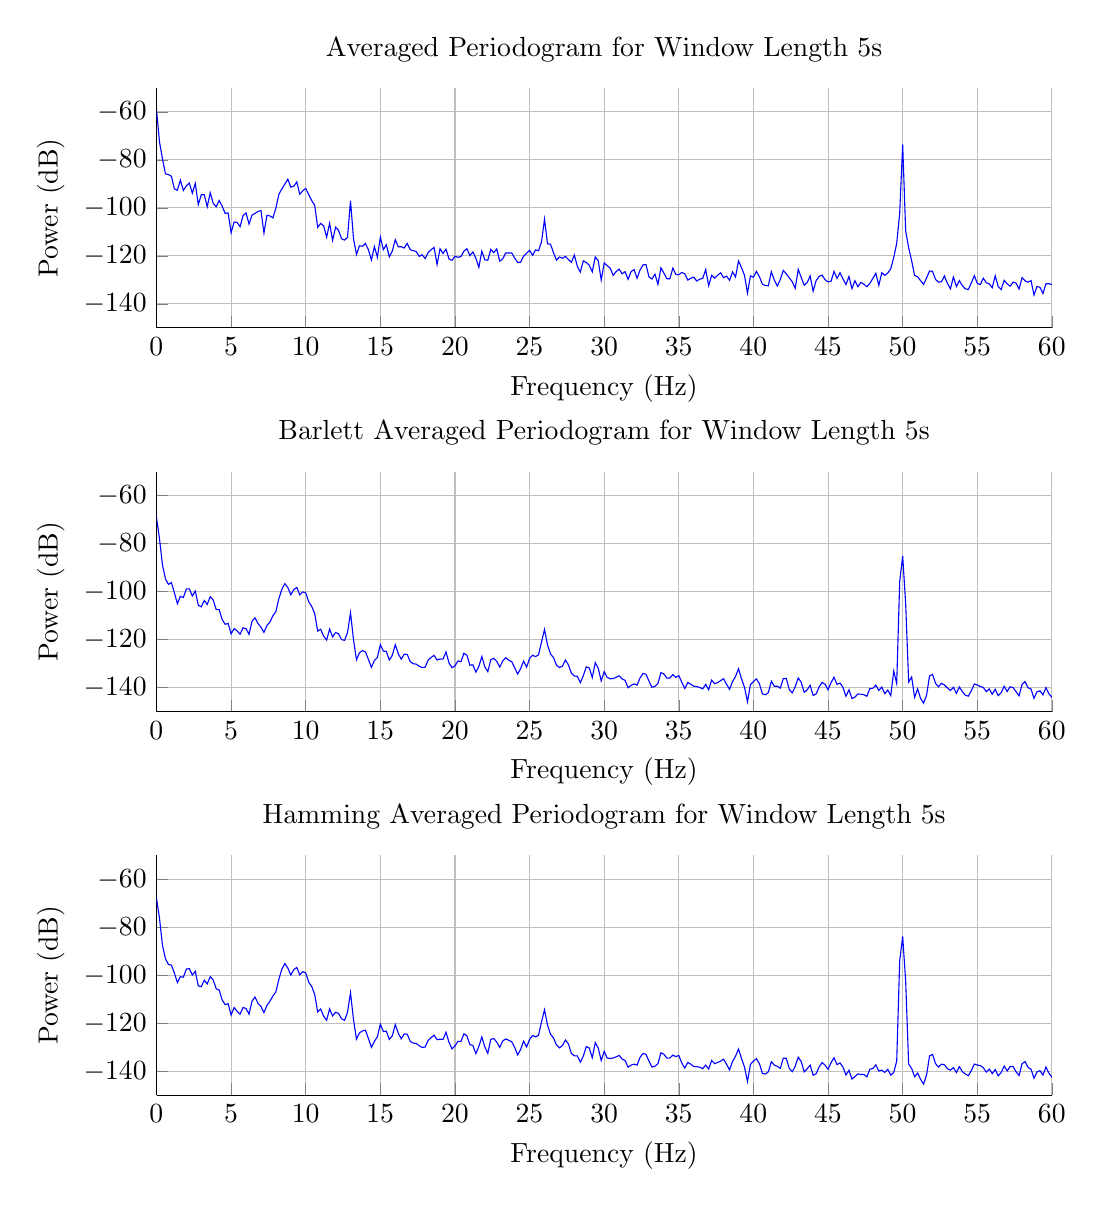
\begin{tikzpicture}

\begin{axis}[%
width=4.47708333333333in,
height=1.2in,
scale only axis,
xmin=0,
xmax=60,
xlabel={Frequency (Hz)},
xmajorgrids,
ymin=-150,
ymax=-50,
ylabel={Power (dB)},
ymajorgrids,
name=plot2,
title={Barlett Averaged Periodogram for Window Length 5s},
axis x line*=bottom,
axis y line*=left
]
\addplot [color=blue,solid,forget plot]
  table[row sep=crcr]{-600	-164.812899679771\\
-599.8	-164.650096194674\\
-599.6	-162.10743016536\\
-599.4	-159.216506019789\\
-599.2	-162.31601253037\\
-599	-163.950649121659\\
-598.8	-162.378843197501\\
-598.6	-162.270242261985\\
-598.4	-166.431010057233\\
-598.2	-167.510996353072\\
-598	-162.242672409197\\
-597.8	-162.288767456137\\
-597.6	-161.293465532966\\
-597.4	-165.337694806975\\
-597.2	-162.560373240045\\
-597	-163.063260394661\\
-596.8	-161.765051553383\\
-596.6	-162.191524413643\\
-596.4	-161.235870773721\\
-596.2	-163.831193105926\\
-596	-164.301367975257\\
-595.8	-157.777808420806\\
-595.6	-162.523085439533\\
-595.4	-163.519904601759\\
-595.2	-164.06473576823\\
-595	-163.727851633321\\
-594.8	-165.320683406978\\
-594.6	-166.853941898411\\
-594.4	-166.321554977315\\
-594.2	-164.755220560603\\
-594	-168.039023391976\\
-593.8	-165.819713977355\\
-593.6	-164.82521696492\\
-593.4	-162.867451682702\\
-593.2	-161.226845965305\\
-593	-163.393299348666\\
-592.8	-162.85696896483\\
-592.6	-165.05054906608\\
-592.4	-166.479451385738\\
-592.2	-162.001220926534\\
-592	-163.689796618149\\
-591.8	-167.581657667072\\
-591.6	-167.077427567119\\
-591.4	-163.528204716597\\
-591.2	-161.288800913203\\
-591	-164.36119348509\\
-590.8	-167.639504727619\\
-590.6	-161.463332439959\\
-590.4	-160.278110102972\\
-590.2	-158.376868733003\\
-590	-163.259526992022\\
-589.8	-166.986427115625\\
-589.6	-164.886066408601\\
-589.4	-164.432491162866\\
-589.2	-161.943674544322\\
-589	-159.378093554424\\
-588.8	-160.893376496681\\
-588.6	-162.535812226845\\
-588.4	-161.994653841035\\
-588.2	-157.22727429218\\
-588	-161.139619116919\\
-587.8	-165.182502699872\\
-587.6	-165.009788637689\\
-587.4	-162.069166427541\\
-587.2	-164.567351699939\\
-587	-161.082549731363\\
-586.8	-161.772480317507\\
-586.6	-164.131453859107\\
-586.4	-163.564168967523\\
-586.2	-165.297275307778\\
-586	-161.295561164403\\
-585.8	-161.267308678051\\
-585.6	-157.72371491399\\
-585.4	-163.198446877363\\
-585.2	-165.048566937488\\
-585	-164.833459997067\\
-584.8	-159.362642824848\\
-584.6	-160.605871815737\\
-584.4	-161.298238487678\\
-584.2	-160.870974169916\\
-584	-160.835550845093\\
-583.8	-160.961277384249\\
-583.6	-160.617849851852\\
-583.4	-161.867233995046\\
-583.2	-161.988625903451\\
-583	-161.860136787715\\
-582.8	-161.336450625829\\
-582.6	-163.218945160648\\
-582.4	-160.047277490348\\
-582.2	-159.731372329054\\
-582	-163.050491246946\\
-581.8	-164.787440685276\\
-581.6	-165.62869432632\\
-581.4	-164.206673964886\\
-581.2	-159.078627092648\\
-581	-160.097077626295\\
-580.8	-165.796301780269\\
-580.6	-167.573406087103\\
-580.4	-162.590894813932\\
-580.2	-165.84269063463\\
-580	-166.623201492344\\
-579.8	-163.712775213857\\
-579.6	-163.348342377446\\
-579.4	-166.211144140839\\
-579.2	-161.024699702661\\
-579	-158.73617274177\\
-578.8	-158.741666237317\\
-578.6	-161.125085576326\\
-578.4	-160.122463938495\\
-578.2	-162.093535764661\\
-578	-166.923575899859\\
-577.8	-165.518110230022\\
-577.6	-167.14832573549\\
-577.4	-166.023411784231\\
-577.2	-162.91163782664\\
-577	-165.140843714409\\
-576.8	-164.736939653012\\
-576.6	-163.262960414173\\
-576.4	-162.631723557444\\
-576.2	-161.824082877517\\
-576	-161.972877343547\\
-575.8	-164.225931426398\\
-575.6	-164.328255029965\\
-575.4	-165.709269973596\\
-575.2	-164.105035707743\\
-575	-159.181026930646\\
-574.8	-160.54599455981\\
-574.6	-160.648124459315\\
-574.4	-162.349992619645\\
-574.2	-162.659552544908\\
-574	-161.203774257083\\
-573.8	-161.441781742189\\
-573.6	-159.761256493888\\
-573.4	-161.478364806319\\
-573.2	-161.296138299321\\
-573	-161.016648788046\\
-572.8	-160.729007123794\\
-572.6	-160.223169895747\\
-572.4	-159.152545317324\\
-572.2	-162.493732642788\\
-572	-161.643767346217\\
-571.8	-162.367999972035\\
-571.6	-164.85406352025\\
-571.4	-162.244529265382\\
-571.2	-163.35114239468\\
-571	-164.824719316535\\
-570.8	-163.490994117321\\
-570.6	-162.216763589892\\
-570.4	-161.688096988972\\
-570.2	-166.287478878394\\
-570	-165.670641455981\\
-569.8	-166.258728952321\\
-569.6	-163.763026959331\\
-569.4	-159.585873669628\\
-569.2	-159.677416079049\\
-569	-161.244532925515\\
-568.8	-160.446557394804\\
-568.6	-161.927856486312\\
-568.4	-161.22309629001\\
-568.2	-163.696924084753\\
-568	-162.056469486674\\
-567.8	-162.460523780295\\
-567.6	-162.990531780075\\
-567.4	-160.315065535738\\
-567.2	-162.904322229586\\
-567	-164.59074263523\\
-566.8	-163.630177877524\\
-566.6	-164.580770707625\\
-566.4	-163.153088285878\\
-566.2	-165.245695431395\\
-566	-166.72532711426\\
-565.8	-164.834892077469\\
-565.6	-162.302544653918\\
-565.4	-158.910671035695\\
-565.2	-157.716226948685\\
-565	-161.563584664373\\
-564.8	-160.321179406344\\
-564.6	-162.254584605166\\
-564.4	-163.801615349992\\
-564.2	-162.425013125385\\
-564	-165.277205835582\\
-563.8	-162.518247939754\\
-563.6	-164.964985628587\\
-563.4	-160.498197094367\\
-563.2	-158.926080218221\\
-563	-165.416222094485\\
-562.8	-162.960096452984\\
-562.6	-162.733220583612\\
-562.4	-161.235958481012\\
-562.2	-163.318683397196\\
-562	-160.239984281811\\
-561.8	-160.103622983941\\
-561.6	-158.472870418781\\
-561.4	-161.190549689569\\
-561.2	-162.330599775651\\
-561	-161.526584557513\\
-560.8	-159.683389775878\\
-560.6	-160.476447234081\\
-560.4	-163.977433824494\\
-560.2	-160.94889632591\\
-560	-160.771270234754\\
-559.8	-160.090360457545\\
-559.6	-158.890302385299\\
-559.4	-159.792533316588\\
-559.2	-165.934522975439\\
-559	-163.603524887635\\
-558.8	-160.433560689794\\
-558.6	-160.11516355642\\
-558.4	-160.8569631279\\
-558.2	-161.748603850777\\
-558	-160.179931291625\\
-557.8	-160.407701488571\\
-557.6	-160.75591873106\\
-557.4	-160.47755477747\\
-557.2	-160.822086779812\\
-557	-161.001434080238\\
-556.8	-164.855768420447\\
-556.6	-163.304494986767\\
-556.4	-159.473648135167\\
-556.2	-160.967832559826\\
-556	-159.969995369939\\
-555.8	-158.127049075628\\
-555.6	-164.71002018693\\
-555.4	-165.044217981346\\
-555.2	-164.778907765811\\
-555	-162.525539546324\\
-554.8	-165.647510728569\\
-554.6	-166.124662112665\\
-554.4	-165.036222797464\\
-554.2	-160.484241950566\\
-554	-162.36300793722\\
-553.8	-161.862864483699\\
-553.6	-157.883649599488\\
-553.4	-156.762095561122\\
-553.2	-158.230506736332\\
-553	-163.209348599735\\
-552.8	-166.025879495904\\
-552.6	-161.086088463876\\
-552.4	-161.918533954699\\
-552.2	-165.318036833397\\
-552	-161.142158965566\\
-551.8	-161.506792157483\\
-551.6	-166.468861496022\\
-551.4	-163.857936175044\\
-551.2	-162.186099271813\\
-551	-163.829739533486\\
-550.8	-161.912516581931\\
-550.6	-152.871855083807\\
-550.4	-149.596042777933\\
-550.2	-150.617286590185\\
-550	-158.910826228752\\
-549.8	-155.243102146448\\
-549.6	-154.188530353023\\
-549.4	-157.928692652876\\
-549.2	-158.612271617806\\
-549	-162.053549274085\\
-548.8	-164.315287888789\\
-548.6	-162.432204743753\\
-548.4	-159.699259750279\\
-548.2	-158.900545557077\\
-548	-163.014349440366\\
-547.8	-163.318044230322\\
-547.6	-159.561494140552\\
-547.4	-163.444100456364\\
-547.2	-163.870070281096\\
-547	-164.31857759963\\
-546.8	-163.922322519641\\
-546.6	-164.091921525333\\
-546.4	-162.04527351388\\
-546.2	-164.489981078169\\
-546	-163.014106448193\\
-545.8	-163.061256724669\\
-545.6	-163.732194468529\\
-545.4	-164.636794649161\\
-545.2	-167.227034599679\\
-545	-161.402063512697\\
-544.8	-159.490244478174\\
-544.6	-161.797480440109\\
-544.4	-160.072294872906\\
-544.2	-158.21154628514\\
-544	-160.344163035641\\
-543.8	-162.736533913729\\
-543.6	-161.896319560133\\
-543.4	-159.844354594068\\
-543.2	-158.063608128637\\
-543	-163.666049180415\\
-542.8	-161.988410772586\\
-542.6	-161.165424348065\\
-542.4	-166.172190196671\\
-542.2	-164.322088383427\\
-542	-164.647385968007\\
-541.8	-158.28533008159\\
-541.6	-162.63566215248\\
-541.4	-162.714910455697\\
-541.2	-160.253347247648\\
-541	-161.554167071843\\
-540.8	-160.224388907165\\
-540.6	-161.904412482594\\
-540.4	-159.585600249381\\
-540.2	-158.935496534592\\
-540	-163.485943519962\\
-539.8	-160.674069608863\\
-539.6	-160.737435305916\\
-539.4	-160.810314035711\\
-539.2	-160.376535484005\\
-539	-159.109533340285\\
-538.8	-159.771303194164\\
-538.6	-163.677073209858\\
-538.4	-168.380410376667\\
-538.2	-164.516173952583\\
-538	-162.122477503413\\
-537.8	-162.729729627341\\
-537.6	-158.681933268325\\
-537.4	-159.798538577863\\
-537.2	-161.002003111228\\
-537	-165.95035955411\\
-536.8	-163.504619714683\\
-536.6	-166.638456554721\\
-536.4	-162.964728071128\\
-536.2	-161.626643075314\\
-536	-160.965533271677\\
-535.8	-164.080294166937\\
-535.6	-162.22057410931\\
-535.4	-160.949434570288\\
-535.2	-166.545077468948\\
-535	-166.80639690231\\
-534.8	-163.579988321096\\
-534.6	-163.357421128658\\
-534.4	-161.860020044023\\
-534.2	-163.696509205583\\
-534	-160.81725370601\\
-533.8	-162.566342438461\\
-533.6	-162.356240490428\\
-533.4	-159.1729426186\\
-533.2	-156.629997983018\\
-533	-160.736974214182\\
-532.8	-160.589878947074\\
-532.6	-160.956898251729\\
-532.4	-164.269932951526\\
-532.2	-157.454331951028\\
-532	-160.771099272937\\
-531.8	-162.271938465369\\
-531.6	-161.883225499357\\
-531.4	-158.533779955609\\
-531.2	-160.851491009828\\
-531	-164.00719200507\\
-530.8	-162.547543400968\\
-530.6	-159.488579374313\\
-530.4	-164.070405800941\\
-530.2	-159.610598250917\\
-530	-161.688558554878\\
-529.8	-161.85992348597\\
-529.6	-160.712243932009\\
-529.4	-162.205609862567\\
-529.2	-160.314202658279\\
-529	-162.640647377641\\
-528.8	-159.445137035227\\
-528.6	-162.290047525356\\
-528.4	-159.760006173881\\
-528.2	-159.951491451607\\
-528	-161.164570245194\\
-527.8	-161.20912129121\\
-527.6	-157.410938433584\\
-527.4	-158.022064156039\\
-527.2	-164.268206305197\\
-527	-162.638522436983\\
-526.8	-161.841216016759\\
-526.6	-160.63435016198\\
-526.4	-165.242236146316\\
-526.2	-161.339574159603\\
-526	-161.921751939219\\
-525.8	-162.164053060184\\
-525.6	-161.451050090583\\
-525.4	-161.716172567047\\
-525.2	-161.293458010889\\
-525	-164.695071101658\\
-524.8	-163.711309646717\\
-524.6	-162.373395797775\\
-524.4	-160.011961213226\\
-524.2	-161.610281423978\\
-524	-157.648089363137\\
-523.8	-162.807233452961\\
-523.6	-163.636391498182\\
-523.4	-161.309036044433\\
-523.2	-161.234640678732\\
-523	-162.806526965234\\
-522.8	-160.956216822844\\
-522.6	-160.108847589605\\
-522.4	-161.483086842913\\
-522.2	-163.536385357465\\
-522	-160.141559153843\\
-521.8	-159.867849976183\\
-521.6	-160.699776869122\\
-521.4	-159.168703895226\\
-521.2	-162.478258954495\\
-521	-166.211883161516\\
-520.8	-158.981983196467\\
-520.6	-160.789695658129\\
-520.4	-162.605068834799\\
-520.2	-162.436614441993\\
-520	-162.310348312209\\
-519.8	-159.140666264316\\
-519.6	-160.561520802567\\
-519.4	-163.25664016714\\
-519.2	-159.647287472266\\
-519	-159.231059962319\\
-518.8	-164.266027164909\\
-518.6	-167.079130474999\\
-518.4	-165.123874492927\\
-518.2	-160.921106355337\\
-518	-157.937511216093\\
-517.8	-163.424622040999\\
-517.6	-164.087923132539\\
-517.4	-162.923963009932\\
-517.2	-162.550760930347\\
-517	-162.44603708494\\
-516.8	-164.783948543556\\
-516.6	-166.477152345287\\
-516.4	-167.672028412282\\
-516.2	-160.138579946167\\
-516	-156.703727511188\\
-515.8	-158.67126053901\\
-515.6	-160.585159622632\\
-515.4	-159.47164366986\\
-515.2	-160.264930124131\\
-515	-162.76966960917\\
-514.8	-161.184538838257\\
-514.6	-160.664132130699\\
-514.4	-162.138808798196\\
-514.2	-164.09928952799\\
-514	-164.834644685499\\
-513.8	-164.002655006821\\
-513.6	-160.99397792443\\
-513.4	-161.708434883768\\
-513.2	-157.669178220665\\
-513	-161.178955147623\\
-512.8	-163.062426386123\\
-512.6	-161.000284056392\\
-512.4	-159.957987282802\\
-512.2	-158.20183815762\\
-512	-161.043038869331\\
-511.8	-161.432956181785\\
-511.6	-166.339397649818\\
-511.4	-162.284194920125\\
-511.2	-163.239985190476\\
-511	-163.859223914838\\
-510.8	-165.375134886865\\
-510.6	-159.832145666501\\
-510.4	-161.229132614469\\
-510.2	-162.645096992986\\
-510	-163.861276334221\\
-509.8	-162.781558916337\\
-509.6	-160.821137682023\\
-509.4	-163.673716677319\\
-509.2	-160.242253500855\\
-509	-157.766377597497\\
-508.8	-159.929017447352\\
-508.6	-161.087019404516\\
-508.4	-160.121071046146\\
-508.2	-157.339532671845\\
-508	-158.934642820094\\
-507.8	-160.136721401239\\
-507.6	-161.890372924399\\
-507.4	-159.27757284388\\
-507.2	-160.285731694398\\
-507	-158.535630002078\\
-506.8	-160.966358939368\\
-506.6	-161.5976245829\\
-506.4	-157.841431299276\\
-506.2	-155.155534880319\\
-506	-158.18874035239\\
-505.8	-157.13393910912\\
-505.6	-162.147516928175\\
-505.4	-160.302050586299\\
-505.2	-155.287017362411\\
-505	-157.826965106881\\
-504.8	-160.028319728221\\
-504.6	-161.442861134107\\
-504.4	-161.878340677339\\
-504.2	-161.610885890014\\
-504	-160.650392363537\\
-503.8	-160.034869165076\\
-503.6	-160.699571965814\\
-503.4	-159.710439870768\\
-503.2	-161.883164894638\\
-503	-163.272642959825\\
-502.8	-159.795064084489\\
-502.6	-164.18363488137\\
-502.4	-162.706870363599\\
-502.2	-163.396389658369\\
-502	-162.262715772723\\
-501.8	-159.480152981105\\
-501.6	-161.146695234948\\
-501.4	-158.598024823878\\
-501.2	-161.883833114372\\
-501	-160.811189584633\\
-500.8	-160.521490887423\\
-500.6	-160.423497585325\\
-500.4	-165.40843594369\\
-500.2	-164.358988208041\\
-500	-160.181869636586\\
-499.8	-159.134889952723\\
-499.6	-159.117843068027\\
-499.4	-160.279430908866\\
-499.2	-156.584410282565\\
-499	-160.007960749558\\
-498.8	-161.167749828069\\
-498.6	-160.346846885345\\
-498.4	-161.513238424714\\
-498.2	-160.806468569133\\
-498	-161.774506300302\\
-497.8	-161.752131058312\\
-497.6	-163.029778188392\\
-497.4	-160.987119828004\\
-497.2	-160.650361193496\\
-497	-159.152346135868\\
-496.8	-162.07310106951\\
-496.6	-161.97974748731\\
-496.4	-163.603450422515\\
-496.2	-162.446484413064\\
-496	-158.672275097803\\
-495.8	-156.80698406734\\
-495.6	-161.325179181285\\
-495.4	-165.586130918194\\
-495.2	-163.843228673655\\
-495	-160.729241756302\\
-494.8	-158.096940946829\\
-494.6	-159.914556968504\\
-494.4	-162.679100590883\\
-494.2	-160.866845806968\\
-494	-161.345178623774\\
-493.8	-161.092709445201\\
-493.6	-163.842495349027\\
-493.4	-165.170273112224\\
-493.2	-166.724382976012\\
-493	-163.607848103088\\
-492.8	-159.82489763834\\
-492.6	-158.344304180189\\
-492.4	-159.128504477125\\
-492.2	-153.947443897478\\
-492	-158.668020582862\\
-491.8	-158.830780469596\\
-491.6	-161.316497152207\\
-491.4	-160.44085025913\\
-491.2	-161.622851552512\\
-491	-163.476601748435\\
-490.8	-161.574073066523\\
-490.6	-160.130429149544\\
-490.4	-165.441573216316\\
-490.2	-164.288904597014\\
-490	-163.111720979297\\
-489.8	-156.399713908195\\
-489.6	-159.530314751172\\
-489.4	-162.376240906193\\
-489.2	-162.108811718023\\
-489	-165.192094932547\\
-488.8	-161.542758601479\\
-488.6	-161.548530466724\\
-488.4	-160.526422881711\\
-488.2	-160.931027383439\\
-488	-157.242973462378\\
-487.8	-159.938612462158\\
-487.6	-159.409510210784\\
-487.4	-158.762654321642\\
-487.2	-157.438906575921\\
-487	-160.345330651144\\
-486.8	-161.587734581505\\
-486.6	-156.055644845606\\
-486.4	-158.122672225289\\
-486.2	-163.427854995268\\
-486	-160.181267572919\\
-485.8	-164.96347908925\\
-485.6	-160.556126177021\\
-485.4	-160.125508928612\\
-485.2	-163.59917449335\\
-485	-160.545077458061\\
-484.8	-162.767870428607\\
-484.6	-160.904279305639\\
-484.4	-160.055315669146\\
-484.2	-159.914953191512\\
-484	-157.721300504987\\
-483.8	-157.405521746547\\
-483.6	-162.314668453438\\
-483.4	-158.243217161577\\
-483.2	-156.906816682051\\
-483	-157.572156796583\\
-482.8	-158.168683444635\\
-482.6	-157.829685324913\\
-482.4	-157.13914750475\\
-482.2	-157.062406687783\\
-482	-161.69931802172\\
-481.8	-158.953303518575\\
-481.6	-160.24517446957\\
-481.4	-159.088511807052\\
-481.2	-158.377470438698\\
-481	-161.512956235029\\
-480.8	-162.860524616428\\
-480.6	-159.191765281185\\
-480.4	-162.640474587688\\
-480.2	-161.533395554468\\
-480	-163.514848005823\\
-479.8	-165.052221576335\\
-479.6	-159.600247503494\\
-479.4	-158.495181774566\\
-479.2	-161.558216817465\\
-479	-167.325486070051\\
-478.8	-164.240390409739\\
-478.6	-165.036863735155\\
-478.4	-160.263591469261\\
-478.2	-162.187400355235\\
-478	-163.627140153816\\
-477.8	-160.808283244554\\
-477.6	-161.514196853354\\
-477.4	-162.242815170913\\
-477.2	-164.001976564609\\
-477	-165.880575227044\\
-476.8	-164.908022376106\\
-476.6	-162.593898690211\\
-476.4	-161.106029346427\\
-476.2	-160.499498723621\\
-476	-159.133228795544\\
-475.8	-164.090293473518\\
-475.6	-160.300261487888\\
-475.4	-159.027277032752\\
-475.2	-161.986910471738\\
-475	-160.338943682215\\
-474.8	-157.992714125498\\
-474.6	-156.786280847712\\
-474.4	-158.214100896271\\
-474.2	-159.92676416577\\
-474	-162.237667380459\\
-473.8	-160.731354712575\\
-473.6	-158.344415477256\\
-473.4	-158.865599115574\\
-473.2	-159.305799048292\\
-473	-156.853892722863\\
-472.8	-159.857977555119\\
-472.6	-159.588273281362\\
-472.4	-159.534691837185\\
-472.2	-157.333765913637\\
-472	-156.61131314887\\
-471.8	-159.749118793626\\
-471.6	-164.816977275063\\
-471.4	-161.396197597602\\
-471.2	-160.765583778481\\
-471	-160.307776348413\\
-470.8	-161.882050281433\\
-470.6	-163.506145210414\\
-470.4	-162.200116861175\\
-470.2	-159.091543514377\\
-470	-161.350404249269\\
-469.8	-159.494543458461\\
-469.6	-159.691042754398\\
-469.4	-159.632256790526\\
-469.2	-158.721713686438\\
-469	-161.9352923317\\
-468.8	-162.046886644505\\
-468.6	-165.290609708527\\
-468.4	-168.163037316635\\
-468.2	-162.304326238929\\
-468	-161.261654633462\\
-467.8	-157.99204165439\\
-467.6	-158.220538768277\\
-467.4	-159.571123465863\\
-467.2	-161.101100062261\\
-467	-162.961224694579\\
-466.8	-160.834005735933\\
-466.6	-159.201282305991\\
-466.4	-157.009665244646\\
-466.2	-159.764683825025\\
-466	-161.844131708755\\
-465.8	-161.322415376881\\
-465.6	-158.407215722605\\
-465.4	-158.884095406355\\
-465.2	-159.59334796827\\
-465	-160.933380357813\\
-464.8	-160.429763030657\\
-464.6	-159.404157500644\\
-464.4	-160.040881992669\\
-464.2	-158.935243763751\\
-464	-161.890593180616\\
-463.8	-165.190899788304\\
-463.6	-160.635320027845\\
-463.4	-157.939239782921\\
-463.2	-161.181851471262\\
-463	-159.873702547173\\
-462.8	-160.614507515557\\
-462.6	-162.764892105112\\
-462.4	-161.816925500229\\
-462.2	-158.108684662048\\
-462	-155.246147215906\\
-461.8	-160.075400123993\\
-461.6	-163.247142166019\\
-461.4	-162.029096830975\\
-461.2	-159.670378837598\\
-461	-161.817599208546\\
-460.8	-160.125990026236\\
-460.6	-163.50838781357\\
-460.4	-162.876209780277\\
-460.2	-160.225041409699\\
-460	-158.129711638427\\
-459.8	-157.83272512431\\
-459.6	-159.49413987095\\
-459.4	-160.053409498765\\
-459.2	-159.51384329555\\
-459	-161.322948402141\\
-458.8	-160.49468004722\\
-458.6	-162.941672729684\\
-458.4	-160.629604609495\\
-458.2	-160.80505612113\\
-458	-159.614910732493\\
-457.8	-158.55566589736\\
-457.6	-160.386320859788\\
-457.4	-163.747863638149\\
-457.2	-160.598439655656\\
-457	-162.33314693905\\
-456.8	-163.419868719422\\
-456.6	-161.474617623891\\
-456.4	-159.902743952594\\
-456.2	-161.934768336123\\
-456	-159.31873575805\\
-455.8	-158.640556201172\\
-455.6	-158.842486831706\\
-455.4	-164.03129567872\\
-455.2	-158.641775530563\\
-455	-159.077192930204\\
-454.8	-161.911277066798\\
-454.6	-159.64368581976\\
-454.4	-158.378162239513\\
-454.2	-157.165300263387\\
-454	-160.268948470219\\
-453.8	-161.087362744678\\
-453.6	-163.306173794749\\
-453.4	-164.633768199157\\
-453.2	-163.380718324042\\
-453	-161.244459732735\\
-452.8	-160.37966127879\\
-452.6	-161.037829419784\\
-452.4	-159.758404640121\\
-452.2	-163.456648585026\\
-452	-159.821893405126\\
-451.8	-163.842015896024\\
-451.6	-162.918903473441\\
-451.4	-162.540196481932\\
-451.2	-161.084566141245\\
-451	-160.601566339525\\
-450.8	-159.764999727971\\
-450.6	-157.0322621536\\
-450.4	-156.386633259331\\
-450.2	-156.813620056326\\
-450	-159.458954985706\\
-449.8	-155.094617174692\\
-449.6	-154.686644726696\\
-449.4	-158.38705885906\\
-449.2	-157.347599214649\\
-449	-157.360672160556\\
-448.8	-159.494744515972\\
-448.6	-157.298557608175\\
-448.4	-160.348947594248\\
-448.2	-162.08640287126\\
-448	-161.247562131723\\
-447.8	-159.229400533375\\
-447.6	-158.696864070826\\
-447.4	-158.206759046277\\
-447.2	-155.806134102921\\
-447	-158.159987040872\\
-446.8	-157.800466869861\\
-446.6	-157.250928101015\\
-446.4	-164.246377804827\\
-446.2	-159.478870979517\\
-446	-158.166884865868\\
-445.8	-157.287854821845\\
-445.6	-159.256990218454\\
-445.4	-161.669207907724\\
-445.2	-157.426914437732\\
-445	-160.844035271722\\
-444.8	-158.655546766692\\
-444.6	-156.272955178885\\
-444.4	-156.981141175549\\
-444.2	-159.444914164208\\
-444	-159.522134669819\\
-443.8	-161.126885197904\\
-443.6	-162.306624213453\\
-443.4	-159.837054900615\\
-443.2	-161.565367331942\\
-443	-160.81099571691\\
-442.8	-159.051264645614\\
-442.6	-157.651581488691\\
-442.4	-159.396691592575\\
-442.2	-156.946782067811\\
-442	-158.060223459412\\
-441.8	-162.110037625229\\
-441.6	-162.616091379271\\
-441.4	-163.356062165069\\
-441.2	-158.344354913684\\
-441	-157.314729294678\\
-440.8	-159.628296672414\\
-440.6	-159.288810228253\\
-440.4	-158.15359525166\\
-440.2	-156.431368094857\\
-440	-157.94774870058\\
-439.8	-159.948725213832\\
-439.6	-159.106917876742\\
-439.4	-161.906692331295\\
-439.2	-159.88012834599\\
-439	-163.410553222048\\
-438.8	-161.071904965811\\
-438.6	-156.921784331023\\
-438.4	-155.616352940462\\
-438.2	-157.352443819081\\
-438	-161.76400061976\\
-437.8	-159.245311699744\\
-437.6	-157.28141231427\\
-437.4	-154.760281010775\\
-437.2	-154.740605020391\\
-437	-154.837142474203\\
-436.8	-154.250281812694\\
-436.6	-157.40733866079\\
-436.4	-161.030984833795\\
-436.2	-163.005888441829\\
-436	-160.576411552818\\
-435.8	-160.336096115456\\
-435.6	-159.504995731025\\
-435.4	-158.272700973152\\
-435.2	-159.834223056323\\
-435	-161.064591673067\\
-434.8	-156.730090915071\\
-434.6	-158.368328568682\\
-434.4	-161.781305639752\\
-434.2	-158.142248665595\\
-434	-157.274301264851\\
-433.8	-159.978749121582\\
-433.6	-159.734091528092\\
-433.4	-156.182132135778\\
-433.2	-160.543804410619\\
-433	-162.460837021147\\
-432.8	-157.687926477532\\
-432.6	-159.046300124113\\
-432.4	-159.669132550472\\
-432.2	-162.079936104998\\
-432	-158.701818952344\\
-431.8	-161.237822532478\\
-431.6	-160.831935356819\\
-431.4	-162.394783886842\\
-431.2	-161.107310991816\\
-431	-159.006287505161\\
-430.8	-157.014478034908\\
-430.6	-162.609205106425\\
-430.4	-163.950800875367\\
-430.2	-157.338974326907\\
-430	-158.983964589565\\
-429.8	-159.330821320256\\
-429.6	-156.403076227215\\
-429.4	-156.388679082148\\
-429.2	-154.663950432107\\
-429	-157.915346668481\\
-428.8	-159.315110585317\\
-428.6	-158.991972426069\\
-428.4	-155.354577455466\\
-428.2	-155.186556975916\\
-428	-157.307760758686\\
-427.8	-156.305236159576\\
-427.6	-157.42500844477\\
-427.4	-160.106032389609\\
-427.2	-160.059941734383\\
-427	-157.804722125576\\
-426.8	-155.804094067805\\
-426.6	-157.759785555435\\
-426.4	-157.344974266332\\
-426.2	-160.850421124172\\
-426	-158.955820804428\\
-425.8	-154.547573579244\\
-425.6	-155.368989081315\\
-425.4	-162.081222793959\\
-425.2	-158.73464465145\\
-425	-156.868626808429\\
-424.8	-157.16232851949\\
-424.6	-159.321193150693\\
-424.4	-160.862807871147\\
-424.2	-158.967463523759\\
-424	-158.123451720999\\
-423.8	-161.192560034806\\
-423.6	-160.049928668058\\
-423.4	-159.687841902466\\
-423.2	-154.995177301585\\
-423	-157.48206739451\\
-422.8	-156.374305103045\\
-422.6	-157.574301079481\\
-422.4	-156.902689967192\\
-422.2	-160.762188337388\\
-422	-161.863676365805\\
-421.8	-157.302832194964\\
-421.6	-158.458873456169\\
-421.4	-160.609613344278\\
-421.2	-156.068747209782\\
-421	-157.712584394323\\
-420.8	-161.356432575893\\
-420.6	-157.034887190025\\
-420.4	-156.036251180514\\
-420.2	-158.501318851592\\
-420	-160.680217739054\\
-419.8	-161.234660928607\\
-419.6	-157.52387243944\\
-419.4	-155.924999896611\\
-419.2	-160.690462581455\\
-419	-157.698969585761\\
-418.8	-158.332480260477\\
-418.6	-160.95478739995\\
-418.4	-161.002434484348\\
-418.2	-159.251695431495\\
-418	-158.782336467664\\
-417.8	-156.779500464427\\
-417.6	-156.565162887823\\
-417.4	-157.981832058083\\
-417.2	-158.511780243103\\
-417	-158.054047625392\\
-416.8	-159.563860172873\\
-416.6	-158.381649671865\\
-416.4	-162.628862534809\\
-416.2	-162.541662769705\\
-416	-160.632566659342\\
-415.8	-162.854673228897\\
-415.6	-158.389971040005\\
-415.4	-154.94643802234\\
-415.2	-156.912084890487\\
-415	-155.267709467067\\
-414.8	-156.384380755472\\
-414.6	-157.091897149125\\
-414.4	-156.768872490538\\
-414.2	-157.12863212511\\
-414	-156.317185808084\\
-413.8	-158.396521745371\\
-413.6	-156.398165223611\\
-413.4	-153.81506307473\\
-413.2	-157.134588027185\\
-413	-156.404394910284\\
-412.8	-156.256833893955\\
-412.6	-158.146300424904\\
-412.4	-158.403743492758\\
-412.2	-159.090606314038\\
-412	-159.339205087365\\
-411.8	-155.827257150049\\
-411.6	-156.908403111289\\
-411.4	-158.0699588013\\
-411.2	-155.055954299478\\
-411	-157.872174787193\\
-410.8	-159.714620327263\\
-410.6	-159.384116927996\\
-410.4	-159.322825159736\\
-410.2	-158.306342548745\\
-410	-161.277661811427\\
-409.8	-156.275199452662\\
-409.6	-158.206942754335\\
-409.4	-156.580367034763\\
-409.2	-160.587431085062\\
-409	-158.623264461597\\
-408.8	-155.665072679525\\
-408.6	-157.904887713539\\
-408.4	-158.633903319283\\
-408.2	-158.969813007335\\
-408	-156.360890587187\\
-407.8	-155.164531076613\\
-407.6	-155.478882814521\\
-407.4	-157.559350253407\\
-407.2	-159.402241949748\\
-407	-158.57626594136\\
-406.8	-155.935833825088\\
-406.6	-159.655587955547\\
-406.4	-159.991807972515\\
-406.2	-160.514032926485\\
-406	-158.432939036751\\
-405.8	-161.961179257492\\
-405.6	-157.228224831808\\
-405.4	-157.694504392528\\
-405.2	-159.616554643368\\
-405	-157.921535242422\\
-404.8	-154.589833122929\\
-404.6	-155.885592356084\\
-404.4	-155.070756514572\\
-404.2	-153.124327152893\\
-404	-154.811669019801\\
-403.8	-158.252583976941\\
-403.6	-156.989232816098\\
-403.4	-154.656660078576\\
-403.2	-155.786415326946\\
-403	-156.872484079886\\
-402.8	-159.726666155264\\
-402.6	-157.814843234906\\
-402.4	-161.201532501389\\
-402.2	-158.489504493696\\
-402	-158.840857200607\\
-401.8	-160.092935650295\\
-401.6	-159.401656266809\\
-401.4	-158.638754398995\\
-401.2	-160.432308705113\\
-401	-162.727113253568\\
-400.8	-157.415517980408\\
-400.6	-157.624890083566\\
-400.4	-157.979540297055\\
-400.2	-163.300280435064\\
-400	-159.089257488277\\
-399.8	-157.517933985612\\
-399.6	-157.97343615753\\
-399.4	-155.222225846886\\
-399.2	-154.371116099889\\
-399	-156.241809854603\\
-398.8	-155.59397977401\\
-398.6	-156.613821244517\\
-398.4	-156.427670679311\\
-398.2	-159.402642153815\\
-398	-159.492297234677\\
-397.8	-155.562363737037\\
-397.6	-157.173079764024\\
-397.4	-156.23195517937\\
-397.2	-155.800228189421\\
-397	-155.755704363244\\
-396.8	-159.292662277409\\
-396.6	-165.7086646428\\
-396.4	-161.257174986201\\
-396.2	-157.126878775519\\
-396	-157.287770564012\\
-395.8	-159.000467890933\\
-395.6	-157.871650179059\\
-395.4	-158.082004687475\\
-395.2	-158.910616913833\\
-395	-158.06078837976\\
-394.8	-157.940935683858\\
-394.6	-158.564135848553\\
-394.4	-160.040946447949\\
-394.2	-157.965926152628\\
-394	-155.16977864211\\
-393.8	-156.165996714899\\
-393.6	-154.681697449609\\
-393.4	-155.413381149659\\
-393.2	-156.558936077738\\
-393	-158.043521286386\\
-392.8	-154.578662328703\\
-392.6	-156.123279600329\\
-392.4	-159.878254655422\\
-392.2	-160.366813686362\\
-392	-157.31692645996\\
-391.8	-157.672690817184\\
-391.6	-157.09137565705\\
-391.4	-155.766564722186\\
-391.2	-154.672192791225\\
-391	-154.100600780632\\
-390.8	-154.745534525355\\
-390.6	-153.598315921602\\
-390.4	-153.529243088992\\
-390.2	-154.490705903891\\
-390	-156.145429801368\\
-389.8	-155.047486140478\\
-389.6	-151.978696647473\\
-389.4	-154.072798976424\\
-389.2	-156.198688620221\\
-389	-154.224412998439\\
-388.8	-155.027643380272\\
-388.6	-155.981984657921\\
-388.4	-155.514892373091\\
-388.2	-154.968788319887\\
-388	-157.650488246284\\
-387.8	-155.491519303034\\
-387.6	-157.949659113519\\
-387.4	-157.24288575665\\
-387.2	-156.890210345167\\
-387	-155.759989217744\\
-386.8	-160.632313995946\\
-386.6	-161.02886841435\\
-386.4	-156.217612223797\\
-386.2	-155.103276066043\\
-386	-154.113131759209\\
-385.8	-151.889745971144\\
-385.6	-155.734729038254\\
-385.4	-155.800623945588\\
-385.2	-153.438243400507\\
-385	-156.938563400366\\
-384.8	-158.275938987962\\
-384.6	-158.051362280651\\
-384.4	-156.667009961489\\
-384.2	-160.29817627467\\
-384	-156.760789177133\\
-383.8	-155.776578935119\\
-383.6	-164.188551462863\\
-383.4	-159.717494878788\\
-383.2	-154.812213939011\\
-383	-155.433406469638\\
-382.8	-155.057630069124\\
-382.6	-156.676972887455\\
-382.4	-158.190301612348\\
-382.2	-156.811888888893\\
-382	-158.156115106717\\
-381.8	-156.048034809595\\
-381.6	-155.64328685806\\
-381.4	-152.59737617281\\
-381.2	-153.058687050584\\
-381	-155.529201601138\\
-380.8	-158.282275340294\\
-380.6	-154.051457365273\\
-380.4	-156.903885489886\\
-380.2	-156.517128374566\\
-380	-155.729903976589\\
-379.8	-154.520997767702\\
-379.6	-154.843866451445\\
-379.4	-154.189577113895\\
-379.2	-157.319078011737\\
-379	-159.159144752973\\
-378.8	-157.293320936009\\
-378.6	-158.510520405667\\
-378.4	-157.54689133241\\
-378.2	-154.872654655872\\
-378	-154.367985712451\\
-377.8	-154.841333416865\\
-377.6	-156.3043808738\\
-377.4	-158.929038802367\\
-377.2	-158.961666484284\\
-377	-158.648424467857\\
-376.8	-159.460731324029\\
-376.6	-154.627089331414\\
-376.4	-153.010365494278\\
-376.2	-154.044782804842\\
-376	-157.341159963779\\
-375.8	-161.426186318839\\
-375.6	-165.240031904913\\
-375.4	-160.23478188061\\
-375.2	-160.385381027531\\
-375	-157.231316747133\\
-374.8	-156.172172918996\\
-374.6	-156.848110569007\\
-374.4	-155.30534282454\\
-374.2	-155.634257079067\\
-374	-155.021616300326\\
-373.8	-156.120917761284\\
-373.6	-155.923191350877\\
-373.4	-156.377065240039\\
-373.2	-156.288236468171\\
-373	-157.525710657737\\
-372.8	-157.140338736302\\
-372.6	-158.990615333937\\
-372.4	-156.03229298498\\
-372.2	-156.10576199551\\
-372	-152.814814420699\\
-371.8	-155.80006393654\\
-371.6	-157.044438199747\\
-371.4	-153.820611110082\\
-371.2	-156.630598330042\\
-371	-157.442806770608\\
-370.8	-158.808562975345\\
-370.6	-155.188541165848\\
-370.4	-156.09303082638\\
-370.2	-156.7669593557\\
-370	-156.160255551211\\
-369.8	-154.353995597542\\
-369.6	-152.164620986815\\
-369.4	-151.783016091807\\
-369.2	-151.967595412834\\
-369	-150.517460360037\\
-368.8	-149.120610723615\\
-368.6	-154.809269424608\\
-368.4	-155.594922559927\\
-368.2	-158.22245425979\\
-368	-154.624676131643\\
-367.8	-156.351482065318\\
-367.6	-155.23421638692\\
-367.4	-154.703129927781\\
-367.2	-156.062312074722\\
-367	-156.503866109708\\
-366.8	-156.974633488556\\
-366.6	-153.575097917665\\
-366.4	-151.650626267774\\
-366.2	-155.277515140119\\
-366	-154.207921777953\\
-365.8	-155.84241052385\\
-365.6	-153.966765449262\\
-365.4	-155.231534327342\\
-365.2	-154.836670909708\\
-365	-157.803292751224\\
-364.8	-159.231681406086\\
-364.6	-161.276561668807\\
-364.4	-157.831736168345\\
-364.2	-152.396444544091\\
-364	-155.197804368727\\
-363.8	-156.144064526515\\
-363.6	-149.721341187164\\
-363.4	-151.607240386183\\
-363.2	-154.460196462364\\
-363	-155.347296468334\\
-362.8	-156.42612438045\\
-362.6	-153.719162519779\\
-362.4	-155.165419885224\\
-362.2	-154.658417950898\\
-362	-156.713934467741\\
-361.8	-160.444934951089\\
-361.6	-160.185627255217\\
-361.4	-159.576564902192\\
-361.2	-157.250380978605\\
-361	-156.373477602421\\
-360.8	-157.003908405879\\
-360.6	-156.875478864504\\
-360.4	-155.250818852658\\
-360.2	-154.61223143416\\
-360	-154.859488746109\\
-359.8	-158.819876392626\\
-359.6	-156.6727452324\\
-359.4	-153.795777856318\\
-359.2	-152.959119623666\\
-359	-152.390097090289\\
-358.8	-156.122375871366\\
-358.6	-158.628121765004\\
-358.4	-157.196696748137\\
-358.2	-155.97513445224\\
-358	-153.541804403216\\
-357.8	-155.10420265826\\
-357.6	-157.295419159836\\
-357.4	-155.099996537944\\
-357.2	-157.821460982908\\
-357	-155.023185959141\\
-356.8	-155.072060159444\\
-356.6	-154.39977802047\\
-356.4	-157.840418725122\\
-356.2	-160.074874471405\\
-356	-157.837437706593\\
-355.8	-155.006729052849\\
-355.6	-155.037431743121\\
-355.4	-151.555689782074\\
-355.2	-151.472273255418\\
-355	-152.598637478901\\
-354.8	-153.576426890304\\
-354.6	-154.213282398085\\
-354.4	-155.72848480081\\
-354.2	-154.808341187545\\
-354	-150.691770071006\\
-353.8	-149.998707603307\\
-353.6	-155.885770776617\\
-353.4	-155.805947205301\\
-353.2	-153.801840999881\\
-353	-155.543797834723\\
-352.8	-155.923367072756\\
-352.6	-155.342920696723\\
-352.4	-155.40435937309\\
-352.2	-151.880910893729\\
-352	-152.417989036772\\
-351.8	-154.702364497725\\
-351.6	-152.588096541877\\
-351.4	-157.743711991101\\
-351.2	-156.615558264343\\
-351	-157.826160682565\\
-350.8	-157.307386360266\\
-350.6	-156.455370483681\\
-350.4	-157.947451542706\\
-350.2	-156.320684047051\\
-350	-150.34400361575\\
-349.8	-150.321368240375\\
-349.6	-155.461528955912\\
-349.4	-158.991830149089\\
-349.2	-157.42545310361\\
-349	-153.507654924613\\
-348.8	-150.752288684646\\
-348.6	-151.946882574959\\
-348.4	-151.597140455085\\
-348.2	-154.330793107484\\
-348	-158.277665388641\\
-347.8	-157.620830775864\\
-347.6	-153.98938500742\\
-347.4	-154.022225611395\\
-347.2	-151.870475437717\\
-347	-152.719088344884\\
-346.8	-154.24370385556\\
-346.6	-156.740420386925\\
-346.4	-154.86719414421\\
-346.2	-155.173071704683\\
-346	-157.540686999289\\
-345.8	-158.11254982446\\
-345.6	-158.820132612464\\
-345.4	-156.181344649723\\
-345.2	-152.573335156016\\
-345	-155.716865291862\\
-344.8	-154.033399232088\\
-344.6	-153.35238964775\\
-344.4	-156.264186954407\\
-344.2	-160.524933798731\\
-344	-155.241377531806\\
-343.8	-154.216181215588\\
-343.6	-157.415693766494\\
-343.4	-153.175383571998\\
-343.2	-150.704075575179\\
-343	-154.351909138792\\
-342.8	-153.592318325886\\
-342.6	-155.380652046668\\
-342.4	-149.745796741723\\
-342.2	-152.188746662884\\
-342	-148.938591311509\\
-341.8	-151.757476178517\\
-341.6	-153.503681731981\\
-341.4	-155.723922770062\\
-341.2	-153.498743976957\\
-341	-157.214155077615\\
-340.8	-156.97320685884\\
-340.6	-152.743851502175\\
-340.4	-152.308527724668\\
-340.2	-156.873323704505\\
-340	-154.56249622784\\
-339.8	-159.453620393948\\
-339.6	-156.391250277481\\
-339.4	-153.554446693345\\
-339.2	-154.459649576694\\
-339	-154.365119040437\\
-338.8	-152.892210907506\\
-338.6	-152.445114332822\\
-338.4	-155.114475701596\\
-338.2	-158.244426623435\\
-338	-155.469949470178\\
-337.8	-152.648421915005\\
-337.6	-153.03428487566\\
-337.4	-154.447412545604\\
-337.2	-149.378714678865\\
-337	-153.017369391625\\
-336.8	-154.845981802138\\
-336.6	-155.547970433307\\
-336.4	-156.188286286111\\
-336.2	-153.741986752354\\
-336	-154.544692857677\\
-335.8	-157.806018533189\\
-335.6	-153.782753055228\\
-335.4	-153.367430751991\\
-335.2	-151.747558767107\\
-335	-153.211400353698\\
-334.8	-155.274294876811\\
-334.6	-154.460536471971\\
-334.4	-153.819177446889\\
-334.2	-156.148265686381\\
-334	-152.964756576701\\
-333.8	-153.852533829965\\
-333.6	-159.468920120101\\
-333.4	-155.358368493037\\
-333.2	-154.634585882406\\
-333	-156.851669951964\\
-332.8	-155.639308285514\\
-332.6	-156.527720560267\\
-332.4	-151.970589704679\\
-332.2	-152.258374701066\\
-332	-153.258069896157\\
-331.8	-156.427300906925\\
-331.6	-154.275087783146\\
-331.4	-153.210951282418\\
-331.2	-157.20465843485\\
-331	-156.691280419421\\
-330.8	-154.788897415992\\
-330.6	-150.923184289169\\
-330.4	-153.164394862826\\
-330.2	-152.465587880219\\
-330	-151.875409949531\\
-329.8	-153.645281242566\\
-329.6	-153.002182247509\\
-329.4	-151.834907621078\\
-329.2	-152.520565338741\\
-329	-152.992195012553\\
-328.8	-155.23361093408\\
-328.6	-155.643572138181\\
-328.4	-153.522118691161\\
-328.2	-153.363713663976\\
-328	-158.814769077841\\
-327.8	-157.229247089997\\
-327.6	-153.324885106571\\
-327.4	-151.838079365523\\
-327.2	-151.987835875707\\
-327	-155.656958400428\\
-326.8	-157.554377775718\\
-326.6	-155.662716672906\\
-326.4	-151.788766189516\\
-326.2	-153.309776421326\\
-326	-152.988537976311\\
-325.8	-152.743086273664\\
-325.6	-153.353595102504\\
-325.4	-152.98851403872\\
-325.2	-151.794771430454\\
-325	-148.111131212023\\
-324.8	-153.600948583909\\
-324.6	-153.234761242829\\
-324.4	-148.738940266477\\
-324.2	-151.109072948352\\
-324	-151.906258969026\\
-323.8	-155.52798776199\\
-323.6	-154.514966477839\\
-323.4	-153.79066122019\\
-323.2	-154.723362901188\\
-323	-154.517236538125\\
-322.8	-154.56966560505\\
-322.6	-153.815621251976\\
-322.4	-152.528601543285\\
-322.2	-151.021430926226\\
-322	-152.235388114758\\
-321.8	-154.774286582884\\
-321.6	-152.013488239216\\
-321.4	-151.680556948744\\
-321.2	-153.475118104821\\
-321	-150.893572152847\\
-320.8	-155.417347027859\\
-320.6	-153.585990936306\\
-320.4	-154.66666923111\\
-320.2	-151.863727846671\\
-320	-148.766308805128\\
-319.8	-151.689490153849\\
-319.6	-151.550012327349\\
-319.4	-154.758540094897\\
-319.2	-155.743269806869\\
-319	-154.98876195408\\
-318.8	-155.672410362916\\
-318.6	-153.873772067239\\
-318.4	-157.476571460749\\
-318.2	-156.408219907103\\
-318	-154.513227221093\\
-317.8	-153.977279037352\\
-317.6	-157.107493035589\\
-317.4	-155.412334649726\\
-317.2	-153.425377964348\\
-317	-151.518955047336\\
-316.8	-152.481959712479\\
-316.6	-156.525207083643\\
-316.4	-157.165584683678\\
-316.2	-151.990476433347\\
-316	-150.326206024067\\
-315.8	-148.820465605393\\
-315.6	-153.480045283152\\
-315.4	-151.697125911086\\
-315.2	-154.11417260363\\
-315	-152.506330945376\\
-314.8	-154.116549263986\\
-314.6	-152.0912009933\\
-314.4	-148.926412015988\\
-314.2	-151.165835732978\\
-314	-151.511863486359\\
-313.8	-152.969069179179\\
-313.6	-153.799559735808\\
-313.4	-152.259665007528\\
-313.2	-155.5031747573\\
-313	-155.482977740883\\
-312.8	-156.495887677176\\
-312.6	-155.108820391153\\
-312.4	-153.024403429076\\
-312.2	-152.83154623185\\
-312	-153.604247511169\\
-311.8	-154.761452581593\\
-311.6	-154.913377105789\\
-311.4	-153.606166193319\\
-311.2	-155.93249916441\\
-311	-155.192000432201\\
-310.8	-156.72982762345\\
-310.6	-155.919286478783\\
-310.4	-154.917985403245\\
-310.2	-152.678489483188\\
-310	-152.65964228033\\
-309.8	-156.119977909151\\
-309.6	-156.557707061757\\
-309.4	-154.267548642491\\
-309.2	-150.793828144747\\
-309	-151.609534118144\\
-308.8	-153.62186005575\\
-308.6	-153.739235204183\\
-308.4	-154.615502661029\\
-308.2	-153.759154255914\\
-308	-154.290218820984\\
-307.8	-152.523447530567\\
-307.6	-150.840195038392\\
-307.4	-155.396952321084\\
-307.2	-153.554400175705\\
-307	-152.912628657591\\
-306.8	-150.7180773312\\
-306.6	-151.76568899859\\
-306.4	-152.142133091022\\
-306.2	-150.719332168412\\
-306	-150.936209266732\\
-305.8	-150.601065000802\\
-305.6	-150.08651053541\\
-305.4	-150.527050578342\\
-305.2	-153.273969099814\\
-305	-153.637042769802\\
-304.8	-148.826627854328\\
-304.6	-148.019502050145\\
-304.4	-147.851727295289\\
-304.2	-149.866837916535\\
-304	-150.841237494262\\
-303.8	-152.47230708761\\
-303.6	-155.611281606791\\
-303.4	-155.330792320806\\
-303.2	-151.338822515864\\
-303	-152.569443196823\\
-302.8	-150.950086810368\\
-302.6	-152.294332538896\\
-302.4	-152.667807213563\\
-302.2	-148.946068620433\\
-302	-154.005121029299\\
-301.8	-152.247400296463\\
-301.6	-152.445483274385\\
-301.4	-151.320738006149\\
-301.2	-153.018470961732\\
-301	-153.385988832355\\
-300.8	-151.659400534172\\
-300.6	-154.927597003901\\
-300.4	-153.851063257209\\
-300.2	-153.863689078183\\
-300	-152.791399016885\\
-299.8	-153.47057676621\\
-299.6	-152.39816400744\\
-299.4	-150.118233628438\\
-299.2	-151.94629034493\\
-299	-155.96222928041\\
-298.8	-153.801919642948\\
-298.6	-152.679631367463\\
-298.4	-155.68142975743\\
-298.2	-151.946503249227\\
-298	-151.790861597006\\
-297.8	-152.524258127265\\
-297.6	-154.881485502943\\
-297.4	-156.253372401902\\
-297.2	-154.209350651503\\
-297	-153.188301869803\\
-296.8	-155.739536210435\\
-296.6	-157.342803704747\\
-296.4	-152.774281608891\\
-296.2	-153.953066357178\\
-296	-150.718743105914\\
-295.8	-152.582018388288\\
-295.6	-152.523983147933\\
-295.4	-152.812905016571\\
-295.2	-151.119696097927\\
-295	-153.472435913746\\
-294.8	-152.899077532388\\
-294.6	-151.992627189429\\
-294.4	-150.684462473718\\
-294.2	-149.02013441108\\
-294	-150.328712983669\\
-293.8	-155.013634970784\\
-293.6	-153.524305119625\\
-293.4	-154.59281657377\\
-293.2	-154.09940427629\\
-293	-153.140459344086\\
-292.8	-154.114154349279\\
-292.6	-153.363547913869\\
-292.4	-153.18255207201\\
-292.2	-153.179817773692\\
-292	-150.993863875838\\
-291.8	-152.471879051905\\
-291.6	-149.990319683222\\
-291.4	-151.366547486747\\
-291.2	-154.544407356928\\
-291	-149.542462223624\\
-290.8	-153.37573480726\\
-290.6	-151.85769076501\\
-290.4	-152.034295238177\\
-290.2	-150.88894240917\\
-290	-154.279197281519\\
-289.8	-150.560748768669\\
-289.6	-151.479803450145\\
-289.4	-149.790844506065\\
-289.2	-145.731206454487\\
-289	-150.588387177693\\
-288.8	-153.38361088281\\
-288.6	-156.678171683346\\
-288.4	-149.862175906304\\
-288.2	-150.989704297646\\
-288	-152.374716977629\\
-287.8	-152.739303703673\\
-287.6	-151.763987502101\\
-287.4	-155.619698005515\\
-287.2	-154.183052502993\\
-287	-156.41197071888\\
-286.8	-153.689180259911\\
-286.6	-148.642324344356\\
-286.4	-151.368986608015\\
-286.2	-149.166653230456\\
-286	-152.248137923383\\
-285.8	-153.090467458267\\
-285.6	-154.254397965862\\
-285.4	-153.41949340483\\
-285.2	-158.587157941411\\
-285	-152.18944153081\\
-284.8	-151.693816278212\\
-284.6	-150.48695308249\\
-284.4	-149.967260357589\\
-284.2	-151.817405684655\\
-284	-149.26040160857\\
-283.8	-154.26767921978\\
-283.6	-153.41127117183\\
-283.4	-154.138832755647\\
-283.2	-151.832769467595\\
-283	-150.958874210314\\
-282.8	-151.794378085271\\
-282.6	-153.636148138887\\
-282.4	-152.587379796013\\
-282.2	-151.358986427168\\
-282	-147.812258328784\\
-281.8	-147.975080965086\\
-281.6	-150.760135497859\\
-281.4	-154.344497938902\\
-281.2	-152.476837421838\\
-281	-147.427878314874\\
-280.8	-147.647833072436\\
-280.6	-149.485722659508\\
-280.4	-152.781325679321\\
-280.2	-151.279347906086\\
-280	-154.279123833681\\
-279.8	-155.10543854762\\
-279.6	-152.469518497277\\
-279.4	-150.371351294062\\
-279.2	-149.812514212397\\
-279	-152.647947918217\\
-278.8	-150.389385586614\\
-278.6	-147.294038809383\\
-278.4	-150.762539919982\\
-278.2	-151.496993616667\\
-278	-152.055882114251\\
-277.8	-150.856461967556\\
-277.6	-153.350685189295\\
-277.4	-154.177495909096\\
-277.2	-151.028011692708\\
-277	-151.745050111272\\
-276.8	-151.864993754709\\
-276.6	-152.855020500084\\
-276.4	-151.222057273142\\
-276.2	-151.598562692395\\
-276	-153.94858623904\\
-275.8	-152.402082366413\\
-275.6	-149.215646490127\\
-275.4	-150.175517330248\\
-275.2	-151.186293707344\\
-275	-153.275377979638\\
-274.8	-153.290296096283\\
-274.6	-148.014604688883\\
-274.4	-151.570079825243\\
-274.2	-153.444199156317\\
-274	-152.159079650522\\
-273.8	-151.316756251227\\
-273.6	-152.751233829747\\
-273.4	-152.364062087438\\
-273.2	-148.774593464208\\
-273	-152.251791402426\\
-272.8	-151.145412641513\\
-272.6	-150.784419569485\\
-272.4	-150.812969877614\\
-272.2	-149.335794290352\\
-272	-149.270489736194\\
-271.8	-149.685301555578\\
-271.6	-151.288494374249\\
-271.4	-152.813879152057\\
-271.2	-151.066687723926\\
-271	-150.586560512918\\
-270.8	-151.088923117967\\
-270.6	-153.868966591314\\
-270.4	-150.167689529169\\
-270.2	-149.13629712925\\
-270	-149.373820796964\\
-269.8	-150.492008800767\\
-269.6	-149.688669137199\\
-269.4	-150.004586056685\\
-269.2	-150.584588452509\\
-269	-151.348179817019\\
-268.8	-149.481495248955\\
-268.6	-150.339623045906\\
-268.4	-151.089715595063\\
-268.2	-148.599398985322\\
-268	-150.496280536188\\
-267.8	-150.932326859558\\
-267.6	-151.920769129356\\
-267.4	-151.265743934837\\
-267.2	-147.085055582783\\
-267	-148.626414867155\\
-266.8	-150.83413562328\\
-266.6	-152.155359552799\\
-266.4	-151.996119076085\\
-266.2	-148.741876387813\\
-266	-147.703770396144\\
-265.8	-151.673926104922\\
-265.6	-149.996750601339\\
-265.4	-149.371458028953\\
-265.2	-152.313944389892\\
-265	-147.444157863752\\
-264.8	-147.768392464258\\
-264.6	-148.222280405113\\
-264.4	-152.078814788049\\
-264.2	-153.390713822418\\
-264	-153.827921711189\\
-263.8	-151.841800927925\\
-263.6	-151.907533858587\\
-263.4	-147.933795577851\\
-263.2	-149.172366456819\\
-263	-154.493181268245\\
-262.8	-152.60130646052\\
-262.6	-150.830906731408\\
-262.4	-149.624639890242\\
-262.2	-152.686023130852\\
-262	-154.908202717103\\
-261.8	-150.10062255502\\
-261.6	-149.526725844022\\
-261.4	-149.370593577125\\
-261.2	-146.863328997745\\
-261	-147.614763650434\\
-260.8	-146.15859678084\\
-260.6	-150.882331877992\\
-260.4	-158.085655062144\\
-260.2	-149.950375637599\\
-260	-149.707386302452\\
-259.8	-152.949714175635\\
-259.6	-153.186353652399\\
-259.4	-152.24451995125\\
-259.2	-149.864794969226\\
-259	-153.482884893044\\
-258.8	-152.205418345821\\
-258.6	-151.131915008605\\
-258.4	-152.310619842822\\
-258.2	-147.597405842215\\
-258	-145.528945883851\\
-257.8	-146.719582937024\\
-257.6	-151.835572192985\\
-257.4	-154.837160892408\\
-257.2	-150.70906736745\\
-257	-149.085117734896\\
-256.8	-151.235778945084\\
-256.6	-149.549815016426\\
-256.4	-147.257373777986\\
-256.2	-153.313218787453\\
-256	-151.770827413338\\
-255.8	-150.324114858996\\
-255.6	-154.413288753139\\
-255.4	-151.045067497945\\
-255.2	-149.040772446703\\
-255	-153.516485590635\\
-254.8	-151.154059701325\\
-254.6	-150.774778243552\\
-254.4	-148.783062775808\\
-254.2	-151.967560805935\\
-254	-151.07897740648\\
-253.8	-150.304460256945\\
-253.6	-153.254466197791\\
-253.4	-150.883159966385\\
-253.2	-152.352877537323\\
-253	-155.978600714607\\
-252.8	-150.985795469164\\
-252.6	-148.884071397002\\
-252.4	-149.151583188576\\
-252.2	-149.603830381988\\
-252	-147.097058968374\\
-251.8	-146.184767666835\\
-251.6	-145.989276147678\\
-251.4	-148.371514242332\\
-251.2	-150.146313893\\
-251	-147.876623696523\\
-250.8	-149.007072139103\\
-250.6	-150.40505979659\\
-250.4	-149.142248109708\\
-250.2	-151.79523792372\\
-250	-139.729057135078\\
-249.8	-133.805712331076\\
-249.6	-145.065618145851\\
-249.4	-148.668848715521\\
-249.2	-148.100619263063\\
-249	-148.980796381595\\
-248.8	-152.465035196237\\
-248.6	-151.149348668182\\
-248.4	-149.687492775687\\
-248.2	-148.654959343859\\
-248	-148.944366074323\\
-247.8	-152.973116245051\\
-247.6	-149.214718486316\\
-247.4	-147.533376654755\\
-247.2	-154.816467745683\\
-247	-153.87704488668\\
-246.8	-149.802769324034\\
-246.6	-147.626019999278\\
-246.4	-152.819135532917\\
-246.2	-150.605730662565\\
-246	-149.516906954672\\
-245.8	-146.786393543934\\
-245.6	-147.146989894214\\
-245.4	-146.014342909959\\
-245.2	-146.536362065247\\
-245	-146.935844353101\\
-244.8	-147.262929528593\\
-244.6	-152.670893375204\\
-244.4	-150.265617833888\\
-244.2	-149.719935217656\\
-244	-150.78910949226\\
-243.8	-149.099420358875\\
-243.6	-148.91247609171\\
-243.4	-151.917951755064\\
-243.2	-151.104419489819\\
-243	-149.708631266149\\
-242.8	-150.839949126886\\
-242.6	-150.46086180245\\
-242.4	-150.226411230738\\
-242.2	-150.824244402883\\
-242	-147.417606207478\\
-241.8	-151.390800914688\\
-241.6	-147.97238590991\\
-241.4	-148.638857022206\\
-241.2	-151.95528382938\\
-241	-150.183568039199\\
-240.8	-152.641981568179\\
-240.6	-152.365190128759\\
-240.4	-149.472673568252\\
-240.2	-150.450965014918\\
-240	-148.336216017031\\
-239.8	-149.653256542682\\
-239.6	-148.936756466639\\
-239.4	-148.614970853245\\
-239.2	-146.713532099451\\
-239	-148.645555352487\\
-238.8	-146.849367682356\\
-238.6	-151.306825605276\\
-238.4	-148.656314338945\\
-238.2	-149.126962060871\\
-238	-151.0095239927\\
-237.8	-151.603903036001\\
-237.6	-149.280954404801\\
-237.4	-150.250347699236\\
-237.2	-146.372252955362\\
-237	-150.459273892122\\
-236.8	-151.932005351962\\
-236.6	-151.984724388706\\
-236.4	-155.304122572818\\
-236.2	-151.421939983226\\
-236	-146.980159106124\\
-235.8	-146.636349597125\\
-235.6	-146.417833731167\\
-235.4	-148.007666149585\\
-235.2	-146.466854146211\\
-235	-149.82620914631\\
-234.8	-149.680478253593\\
-234.6	-152.783583822559\\
-234.4	-152.077131967668\\
-234.2	-148.639602517281\\
-234	-148.099963009066\\
-233.8	-155.562962888265\\
-233.6	-156.168618244665\\
-233.4	-151.995504894463\\
-233.2	-149.357304541261\\
-233	-147.452353009682\\
-232.8	-145.94082133519\\
-232.6	-145.558941479512\\
-232.4	-148.076827302566\\
-232.2	-152.821880372063\\
-232	-150.893442190735\\
-231.8	-150.565111568775\\
-231.6	-152.135908913911\\
-231.4	-146.726831941339\\
-231.2	-143.562778728491\\
-231	-147.425793154031\\
-230.8	-148.203683177623\\
-230.6	-150.62208469185\\
-230.4	-148.513203378299\\
-230.2	-150.805943162314\\
-230	-149.466284882205\\
-229.8	-150.193804096906\\
-229.6	-150.629640735841\\
-229.4	-148.124036087986\\
-229.2	-147.637337540956\\
-229	-148.919853957682\\
-228.8	-148.009725628264\\
-228.6	-146.415395555923\\
-228.4	-150.333378071154\\
-228.2	-151.467884481147\\
-228	-148.65142392762\\
-227.8	-149.714447926492\\
-227.6	-152.877875710127\\
-227.4	-147.01643785229\\
-227.2	-145.700500945367\\
-227	-150.09200952053\\
-226.8	-147.501372471307\\
-226.6	-149.241905321833\\
-226.4	-149.634706216188\\
-226.2	-149.454808940429\\
-226	-155.52665928111\\
-225.8	-148.737185283575\\
-225.6	-148.273323014328\\
-225.4	-150.415876822481\\
-225.2	-145.60081431933\\
-225	-146.034306650107\\
-224.8	-146.041498456055\\
-224.6	-151.556475003869\\
-224.4	-150.705618579522\\
-224.2	-145.170653535734\\
-224	-149.561953286157\\
-223.8	-150.584462911136\\
-223.6	-148.247483089463\\
-223.4	-145.036658453331\\
-223.2	-149.574183308858\\
-223	-148.181153514717\\
-222.8	-147.715823851855\\
-222.6	-149.787879884781\\
-222.4	-149.564441284755\\
-222.2	-146.881384882354\\
-222	-148.500155616494\\
-221.8	-150.791109110444\\
-221.6	-148.052559164657\\
-221.4	-145.098248454232\\
-221.2	-149.712263999776\\
-221	-156.860237872237\\
-220.8	-150.765279585491\\
-220.6	-145.997327605366\\
-220.4	-144.814534146903\\
-220.2	-147.515545882156\\
-220	-152.097942448012\\
-219.8	-150.782056867597\\
-219.6	-151.636008296503\\
-219.4	-150.015428615745\\
-219.2	-146.819363044342\\
-219	-149.645012314169\\
-218.8	-147.719751385885\\
-218.6	-149.386292962909\\
-218.4	-148.230491308281\\
-218.2	-147.853748006493\\
-218	-149.579989159295\\
-217.8	-150.438751637345\\
-217.6	-149.743636701306\\
-217.4	-150.855441737111\\
-217.2	-151.116715416222\\
-217	-144.425194575873\\
-216.8	-144.702130134992\\
-216.6	-146.706972274445\\
-216.4	-147.265187323473\\
-216.2	-146.714591495608\\
-216	-147.691648082344\\
-215.8	-149.423110994821\\
-215.6	-148.036145204418\\
-215.4	-145.137757039288\\
-215.2	-145.598918734998\\
-215	-151.328634009043\\
-214.8	-153.266244719972\\
-214.6	-149.682532545\\
-214.4	-149.941663099265\\
-214.2	-149.84891981441\\
-214	-149.051289024074\\
-213.8	-147.385986569575\\
-213.6	-145.55863043026\\
-213.4	-146.215666009768\\
-213.2	-145.58858604217\\
-213	-143.157150449922\\
-212.8	-145.062726902883\\
-212.6	-143.572311444727\\
-212.4	-148.6767611634\\
-212.2	-149.1555797625\\
-212	-147.164095368033\\
-211.8	-144.902684519214\\
-211.6	-143.278538044064\\
-211.4	-144.329989610065\\
-211.2	-144.992302711487\\
-211	-143.201952665932\\
-210.8	-144.797332961207\\
-210.6	-146.0126068299\\
-210.4	-143.937159522097\\
-210.2	-147.682694119572\\
-210	-146.74969256861\\
-209.8	-147.714210207673\\
-209.6	-151.137196709395\\
-209.4	-150.277150504711\\
-209.2	-148.643828085333\\
-209	-151.855635374964\\
-208.8	-144.821784272823\\
-208.6	-145.723005115751\\
-208.4	-144.028983497576\\
-208.2	-145.640826578475\\
-208	-146.740210669434\\
-207.8	-143.691625671387\\
-207.6	-145.646304827222\\
-207.4	-148.441945898009\\
-207.2	-147.798934650023\\
-207	-147.50703817086\\
-206.8	-145.535778570565\\
-206.6	-146.827638040105\\
-206.4	-149.215446006157\\
-206.2	-150.378737514381\\
-206	-145.057391984094\\
-205.8	-146.951697394472\\
-205.6	-147.558125562481\\
-205.4	-147.253630300118\\
-205.2	-144.127545134476\\
-205	-147.691474678039\\
-204.8	-150.358206691659\\
-204.6	-149.390751994972\\
-204.4	-148.35028900317\\
-204.2	-146.317621696812\\
-204	-145.461394214532\\
-203.8	-145.358444140918\\
-203.6	-145.195208632025\\
-203.4	-143.399613031175\\
-203.2	-147.866464855566\\
-203	-143.865599813766\\
-202.8	-146.931523131512\\
-202.6	-148.854787100595\\
-202.4	-148.714450231814\\
-202.2	-148.15807713315\\
-202	-146.465823631344\\
-201.8	-147.158862543044\\
-201.6	-145.739403016762\\
-201.4	-142.429065902702\\
-201.2	-143.520183497121\\
-201	-142.821574775976\\
-200.8	-141.645191677218\\
-200.6	-144.661865208726\\
-200.4	-147.370810893556\\
-200.2	-149.095123458816\\
-200	-147.243529534351\\
-199.8	-146.815048260383\\
-199.6	-148.284686135504\\
-199.4	-148.151736615843\\
-199.2	-146.647658562231\\
-199	-146.708319818495\\
-198.8	-142.267243305597\\
-198.6	-145.698114134932\\
-198.4	-146.461600418464\\
-198.2	-144.906253422431\\
-198	-145.27060287227\\
-197.8	-145.407380661437\\
-197.6	-149.185942328201\\
-197.4	-147.060600163973\\
-197.2	-141.961720413321\\
-197	-144.005263063573\\
-196.8	-145.217938837469\\
-196.6	-147.793518316238\\
-196.4	-146.654247531254\\
-196.2	-148.435141243315\\
-196	-148.871809622707\\
-195.8	-149.994557717313\\
-195.6	-149.341840101877\\
-195.4	-149.865949556104\\
-195.2	-146.085626311673\\
-195	-146.545906527925\\
-194.8	-149.60140097826\\
-194.6	-152.835930989737\\
-194.4	-149.628759034743\\
-194.2	-145.732468078601\\
-194	-144.524487842989\\
-193.8	-146.715557028531\\
-193.6	-148.25056102052\\
-193.4	-145.91848097375\\
-193.2	-146.431937345488\\
-193	-146.745316906394\\
-192.8	-144.875147004491\\
-192.6	-144.923163302845\\
-192.4	-144.483742289033\\
-192.2	-147.004867041624\\
-192	-146.096671696033\\
-191.8	-145.825916619149\\
-191.6	-147.363978622001\\
-191.4	-150.446777348767\\
-191.2	-148.782796282132\\
-191	-152.746951111826\\
-190.8	-149.055615848565\\
-190.6	-145.981461136279\\
-190.4	-146.578768799596\\
-190.2	-142.145204231655\\
-190	-148.305760546812\\
-189.8	-147.272048534891\\
-189.6	-143.155111965761\\
-189.4	-144.949086229985\\
-189.2	-152.351197424464\\
-189	-148.14880071565\\
-188.8	-146.784386981981\\
-188.6	-149.285441595722\\
-188.4	-145.872099391197\\
-188.2	-145.463826020833\\
-188	-143.991648062634\\
-187.8	-143.97784332596\\
-187.6	-142.923014067808\\
-187.4	-145.705591785109\\
-187.2	-144.161438022847\\
-187	-146.012408501102\\
-186.8	-148.80524113705\\
-186.6	-147.187199632941\\
-186.4	-148.149296618528\\
-186.2	-146.171215045002\\
-186	-147.507596812015\\
-185.8	-149.146660338214\\
-185.6	-144.725332412617\\
-185.4	-144.945553624224\\
-185.2	-144.981260776978\\
-185	-147.868281197061\\
-184.8	-146.369553111187\\
-184.6	-144.978703405639\\
-184.4	-143.473815974478\\
-184.2	-144.880834066231\\
-184	-146.426448458212\\
-183.8	-144.787214071221\\
-183.6	-148.848467742251\\
-183.4	-146.168482714334\\
-183.2	-147.905861567382\\
-183	-149.432512188044\\
-182.8	-144.221106925886\\
-182.6	-146.425446429197\\
-182.4	-143.902867738582\\
-182.2	-147.468740049296\\
-182	-146.562018058735\\
-181.8	-147.128303855268\\
-181.6	-144.205594078288\\
-181.4	-143.739040423668\\
-181.2	-147.64590296391\\
-181	-146.434543258151\\
-180.8	-147.557125384914\\
-180.6	-151.351033877682\\
-180.4	-149.785855621155\\
-180.2	-146.568688361993\\
-180	-144.57749021787\\
-179.8	-149.342683445129\\
-179.6	-144.977453570003\\
-179.4	-145.84102794649\\
-179.2	-143.754409687213\\
-179	-144.008652161029\\
-178.8	-147.359744347295\\
-178.6	-144.893166035313\\
-178.4	-143.442225188244\\
-178.2	-144.351603858897\\
-178	-145.393580639158\\
-177.8	-143.563433505911\\
-177.6	-142.520670089521\\
-177.4	-147.754269669718\\
-177.2	-145.602413722322\\
-177	-147.988286498171\\
-176.8	-145.085691967084\\
-176.6	-146.305494380075\\
-176.4	-144.748051431432\\
-176.2	-146.630576656778\\
-176	-145.018336846184\\
-175.8	-144.44834412571\\
-175.6	-146.626585162275\\
-175.4	-144.0781570637\\
-175.2	-143.004734372881\\
-175	-142.129646955731\\
-174.8	-141.718770833603\\
-174.6	-148.437565790264\\
-174.4	-146.483613178484\\
-174.2	-146.694783176833\\
-174	-144.357267969257\\
-173.8	-146.945435349761\\
-173.6	-147.552058323414\\
-173.4	-147.320035531956\\
-173.2	-148.493430229475\\
-173	-148.63233380418\\
-172.8	-145.565211156401\\
-172.6	-146.738116392635\\
-172.4	-144.182065173843\\
-172.2	-147.082251299098\\
-172	-144.737154276764\\
-171.8	-146.988307552711\\
-171.6	-143.698150510876\\
-171.4	-142.36036250655\\
-171.2	-142.901187674206\\
-171	-144.24429475056\\
-170.8	-145.598297115136\\
-170.6	-142.46772744847\\
-170.4	-142.865286504169\\
-170.2	-143.976110729677\\
-170	-141.62116049183\\
-169.8	-140.963374214795\\
-169.6	-143.691298372932\\
-169.4	-143.731492841443\\
-169.2	-146.368448551324\\
-169	-145.983897350992\\
-168.8	-143.802602331442\\
-168.6	-144.39395423671\\
-168.4	-143.248784893412\\
-168.2	-145.034582532287\\
-168	-146.544215192233\\
-167.8	-144.563492116198\\
-167.6	-147.495839829875\\
-167.4	-148.265042024896\\
-167.2	-147.032491455545\\
-167	-147.628573121715\\
-166.8	-144.055409362753\\
-166.6	-145.183929874139\\
-166.4	-143.102536032349\\
-166.2	-146.394770596676\\
-166	-147.941665516626\\
-165.8	-146.977478114451\\
-165.6	-145.634353533579\\
-165.4	-145.059713288673\\
-165.2	-146.786135342141\\
-165	-144.988908037337\\
-164.8	-146.803427642338\\
-164.6	-141.600176231629\\
-164.4	-144.474332125125\\
-164.2	-145.705235513205\\
-164	-144.273510006897\\
-163.8	-147.80549861302\\
-163.6	-145.945115767146\\
-163.4	-146.104989016407\\
-163.2	-147.926257832025\\
-163	-150.922053810806\\
-162.8	-149.11924181996\\
-162.6	-148.158777531414\\
-162.4	-145.727241471934\\
-162.2	-144.606009499456\\
-162	-143.800929881555\\
-161.8	-142.394963265639\\
-161.6	-140.639944225879\\
-161.4	-142.493721914237\\
-161.2	-143.482228551536\\
-161	-142.085736178094\\
-160.8	-142.016866332574\\
-160.6	-140.184156683696\\
-160.4	-142.912004439579\\
-160.2	-143.487577553543\\
-160	-143.257164500948\\
-159.8	-143.882297932472\\
-159.6	-145.350188553457\\
-159.4	-147.170230412191\\
-159.2	-142.217254779764\\
-159	-145.127234103609\\
-158.8	-146.734128721895\\
-158.6	-147.134189532403\\
-158.4	-149.896577199576\\
-158.2	-152.619521904379\\
-158	-147.027531299061\\
-157.8	-145.038616432772\\
-157.6	-144.644843056557\\
-157.4	-143.315808259036\\
-157.2	-146.340443935569\\
-157	-144.952706346403\\
-156.8	-147.602921723395\\
-156.6	-149.563445409614\\
-156.4	-145.355724283034\\
-156.2	-145.976388572407\\
-156	-143.101973133503\\
-155.8	-148.922281175189\\
-155.6	-148.136291745528\\
-155.4	-144.146509956957\\
-155.2	-143.054242386024\\
-155	-143.820395005323\\
-154.8	-140.886561552465\\
-154.6	-141.58828343909\\
-154.4	-141.010097023309\\
-154.2	-142.703129715094\\
-154	-141.851840376275\\
-153.8	-141.845670265764\\
-153.6	-142.024380709831\\
-153.4	-143.408674053037\\
-153.2	-147.252246946807\\
-153	-142.40592481699\\
-152.8	-141.317616690442\\
-152.6	-143.12770289261\\
-152.4	-146.643572082545\\
-152.2	-148.678166703186\\
-152	-148.726866593836\\
-151.8	-144.649700862151\\
-151.6	-145.052448931028\\
-151.4	-145.454358452325\\
-151.2	-144.52457294175\\
-151	-141.138384951741\\
-150.8	-139.774533697661\\
-150.6	-143.276841628508\\
-150.4	-147.748047513414\\
-150.2	-144.454734803463\\
-150	-139.66741730456\\
-149.8	-138.954347885295\\
-149.6	-146.703042305426\\
-149.4	-144.54915695736\\
-149.2	-142.14180669519\\
-149	-144.887212031886\\
-148.8	-147.190085115643\\
-148.6	-149.747702184459\\
-148.4	-145.097899206959\\
-148.2	-144.722873271737\\
-148	-147.023588762479\\
-147.8	-145.667499973957\\
-147.6	-143.001470183837\\
-147.4	-146.366518366918\\
-147.2	-144.273004199649\\
-147	-144.738491272124\\
-146.8	-146.794950910066\\
-146.6	-145.110064295851\\
-146.4	-139.872696984382\\
-146.2	-142.88933144529\\
-146	-142.487915785095\\
-145.8	-143.870035928472\\
-145.6	-142.628830325829\\
-145.4	-142.424292658465\\
-145.2	-144.534307358149\\
-145	-146.179613057961\\
-144.8	-145.854995533759\\
-144.6	-145.189144516935\\
-144.4	-146.030901248839\\
-144.2	-146.197741918445\\
-144	-146.074449165242\\
-143.8	-145.567375990184\\
-143.6	-145.227708189382\\
-143.4	-145.004488444301\\
-143.2	-142.991138953839\\
-143	-143.954291094474\\
-142.8	-142.195943568003\\
-142.6	-141.79568920524\\
-142.4	-145.287493660781\\
-142.2	-142.701660871179\\
-142	-143.682373768631\\
-141.8	-146.746557888283\\
-141.6	-143.383842297034\\
-141.4	-141.96390627659\\
-141.2	-145.453798922174\\
-141	-143.171408322635\\
-140.8	-142.762215553876\\
-140.6	-141.236671095088\\
-140.4	-138.771561265471\\
-140.2	-139.442291668345\\
-140	-141.682666999119\\
-139.8	-142.810800196685\\
-139.6	-143.213034531697\\
-139.4	-142.990936926584\\
-139.2	-142.147752251654\\
-139	-142.927376900707\\
-138.8	-141.145222194217\\
-138.6	-142.175692568583\\
-138.4	-144.339391090216\\
-138.2	-143.523776688418\\
-138	-144.915501293628\\
-137.8	-145.326444159137\\
-137.6	-143.920851945097\\
-137.4	-144.531799543559\\
-137.2	-146.689513138559\\
-137	-145.948041768514\\
-136.8	-147.501984622064\\
-136.6	-142.64228721492\\
-136.4	-144.872572458938\\
-136.2	-144.750947239645\\
-136	-142.940351323079\\
-135.8	-141.729344054597\\
-135.6	-146.194976070531\\
-135.4	-144.02983093216\\
-135.2	-144.261432340641\\
-135	-141.818542118997\\
-134.8	-145.850576188797\\
-134.6	-145.494745311105\\
-134.4	-141.622626199358\\
-134.2	-140.972701682965\\
-134	-141.676124846402\\
-133.8	-142.028939686367\\
-133.6	-143.139098841011\\
-133.4	-142.268588778778\\
-133.2	-145.687142654264\\
-133	-143.747053486602\\
-132.8	-146.947310765781\\
-132.6	-143.856289826605\\
-132.4	-140.827850427565\\
-132.2	-142.834147110896\\
-132	-142.689612637759\\
-131.8	-141.365981146401\\
-131.6	-146.369496433999\\
-131.4	-148.422391945601\\
-131.2	-146.917926026955\\
-131	-144.786563332646\\
-130.8	-142.817653455144\\
-130.6	-143.231507675737\\
-130.4	-143.510300511734\\
-130.2	-146.518582358878\\
-130	-147.078545077548\\
-129.8	-147.76445951388\\
-129.6	-145.237939983418\\
-129.4	-143.465695934407\\
-129.2	-143.71663686141\\
-129	-144.066412239918\\
-128.8	-144.660340112063\\
-128.6	-138.49318411442\\
-128.4	-140.236010628222\\
-128.2	-144.794893285973\\
-128	-144.613662440202\\
-127.8	-142.610166551501\\
-127.6	-145.880954039134\\
-127.4	-148.170642746219\\
-127.2	-144.811814541333\\
-127	-144.582297060947\\
-126.8	-143.811669575137\\
-126.6	-142.329805380702\\
-126.4	-143.823791732797\\
-126.2	-147.032306459273\\
-126	-141.692494150217\\
-125.8	-139.808207682603\\
-125.6	-141.743678702234\\
-125.4	-145.805006035572\\
-125.2	-145.230100222416\\
-125	-143.142308770871\\
-124.8	-144.208899349871\\
-124.6	-145.286809680057\\
-124.4	-146.94695011686\\
-124.2	-145.494692815049\\
-124	-143.918575136241\\
-123.8	-143.376159393074\\
-123.6	-140.592668244478\\
-123.4	-143.470163309964\\
-123.2	-143.04567568025\\
-123	-139.782106517654\\
-122.8	-142.396364031059\\
-122.6	-144.076214011896\\
-122.4	-143.666693426746\\
-122.2	-143.954555246714\\
-122	-144.202077486954\\
-121.8	-141.761272763359\\
-121.6	-141.54744360222\\
-121.4	-145.355493500864\\
-121.2	-145.537648091329\\
-121	-145.216915396411\\
-120.8	-143.685282244421\\
-120.6	-141.549130647965\\
-120.4	-143.717788932687\\
-120.2	-143.346256265959\\
-120	-143.340709318596\\
-119.8	-145.38302272699\\
-119.6	-144.021357312351\\
-119.4	-144.210224282446\\
-119.2	-141.902109381246\\
-119	-142.985713897337\\
-118.8	-142.933862408625\\
-118.6	-144.255988635266\\
-118.4	-143.603285928661\\
-118.2	-146.046057674214\\
-118	-147.043833449712\\
-117.8	-143.819939415057\\
-117.6	-142.042437146948\\
-117.4	-145.352417998918\\
-117.2	-147.468954309635\\
-117	-144.94090209248\\
-116.8	-144.700700349859\\
-116.6	-144.491571981161\\
-116.4	-142.919946855542\\
-116.2	-145.093504806105\\
-116	-142.432973354534\\
-115.8	-146.658492265394\\
-115.6	-147.211577292449\\
-115.4	-144.242501452866\\
-115.2	-143.011935922269\\
-115	-146.302371219594\\
-114.8	-142.55695683065\\
-114.6	-142.781469051515\\
-114.4	-145.526400431124\\
-114.2	-144.918570795436\\
-114	-141.457667209472\\
-113.8	-141.550362516194\\
-113.6	-143.415507353825\\
-113.4	-143.709907353925\\
-113.2	-144.847032221855\\
-113	-144.746597583598\\
-112.8	-141.711444170544\\
-112.6	-142.175287160962\\
-112.4	-142.833360802725\\
-112.2	-145.633041585601\\
-112	-145.702333808339\\
-111.8	-140.883519317869\\
-111.6	-144.131600187037\\
-111.4	-140.832616633576\\
-111.2	-141.715155447057\\
-111	-143.4753740498\\
-110.8	-137.745183605484\\
-110.6	-139.415998309751\\
-110.4	-140.497469340381\\
-110.2	-145.326835074374\\
-110	-145.647023273952\\
-109.8	-147.420794098592\\
-109.6	-145.759169879369\\
-109.4	-143.332983408349\\
-109.2	-142.90844494565\\
-109	-143.886212842784\\
-108.8	-142.350914118426\\
-108.6	-141.608768539787\\
-108.4	-144.588779341298\\
-108.2	-141.541846596235\\
-108	-137.553987779549\\
-107.8	-141.870967471881\\
-107.6	-143.551919180636\\
-107.4	-142.724326593509\\
-107.2	-144.678873510751\\
-107	-140.721774654221\\
-106.8	-143.27205143521\\
-106.6	-142.134437960315\\
-106.4	-141.952457723394\\
-106.2	-144.113546544693\\
-106	-145.004291148745\\
-105.8	-145.838988993244\\
-105.6	-151.137428395739\\
-105.4	-148.228518359329\\
-105.2	-140.246763241771\\
-105	-142.206987912711\\
-104.8	-146.635672734779\\
-104.6	-144.320526683786\\
-104.4	-145.798828766457\\
-104.2	-142.381914462386\\
-104	-142.988040942155\\
-103.8	-142.568760423059\\
-103.6	-143.125248586519\\
-103.4	-144.233972950651\\
-103.2	-142.605177264401\\
-103	-143.879190827813\\
-102.8	-142.960240513816\\
-102.6	-142.013625504523\\
-102.4	-144.967252643837\\
-102.2	-146.928976508831\\
-102	-145.293698567219\\
-101.8	-148.212090761275\\
-101.6	-140.407318349975\\
-101.4	-139.685769031667\\
-101.2	-139.369916884378\\
-101	-142.586671385371\\
-100.8	-141.732995974409\\
-100.6	-142.511908580376\\
-100.4	-140.873705670027\\
-100.2	-141.497406289144\\
-100	-144.169419915021\\
-99.8	-142.933230176181\\
-99.6	-140.479917610131\\
-99.4	-142.487487352248\\
-99.2	-146.556735983112\\
-99	-143.132385191802\\
-98.8	-143.26770810535\\
-98.6	-142.761327035533\\
-98.4	-145.656277406042\\
-98.2	-145.514941891011\\
-98	-139.892153657778\\
-97.8	-139.560200624886\\
-97.6	-141.75186917826\\
-97.4	-146.043781316401\\
-97.2	-146.638813098879\\
-97	-142.181496842074\\
-96.8	-146.773146687565\\
-96.6	-143.987021365146\\
-96.4	-144.212405413971\\
-96.2	-145.024377192686\\
-96	-144.769117965629\\
-95.8	-143.41444515104\\
-95.6	-142.945576547327\\
-95.4	-140.923743946729\\
-95.2	-139.624800886237\\
-95	-138.599914466814\\
-94.8	-140.43951229656\\
-94.6	-142.027787794069\\
-94.4	-142.756329827056\\
-94.2	-144.721134503712\\
-94	-141.182505286002\\
-93.8	-141.370186707678\\
-93.6	-144.113009038926\\
-93.4	-142.054004378646\\
-93.2	-140.407418666681\\
-93	-140.120229195176\\
-92.8	-143.234153437506\\
-92.6	-145.881369816222\\
-92.4	-143.856777630416\\
-92.2	-147.900746231425\\
-92	-139.64160157781\\
-91.8	-140.419475429843\\
-91.6	-144.030707331764\\
-91.4	-146.798619479998\\
-91.2	-143.882742986801\\
-90.9999999999999	-141.641184344489\\
-90.8	-143.047936561556\\
-90.6	-145.637367769429\\
-90.4	-145.697567043272\\
-90.2	-143.825971533566\\
-90	-143.84313471301\\
-89.8	-143.93801375404\\
-89.6	-143.29375211032\\
-89.4	-143.705985992093\\
-89.2	-144.40728964784\\
-89	-142.705160852374\\
-88.8	-141.344256149837\\
-88.6	-143.118194634453\\
-88.4	-145.785824879426\\
-88.2	-143.835305786127\\
-88	-143.745187618412\\
-87.8	-142.804772221313\\
-87.6	-143.829214945528\\
-87.4	-144.540950460195\\
-87.2	-143.146003264162\\
-87	-143.12977102671\\
-86.8000000000001	-140.026877481939\\
-86.6	-139.222706906184\\
-86.4	-138.884606688897\\
-86.2	-139.296510634876\\
-86	-142.604738630487\\
-85.8	-142.335176874402\\
-85.6	-141.981143522134\\
-85.4	-142.761973279637\\
-85.2	-144.22422498333\\
-85	-144.797251701822\\
-84.8	-143.242177521063\\
-84.6	-142.127388519027\\
-84.4	-144.024091816397\\
-84.1999999999999	-147.723908889286\\
-84	-143.503327851397\\
-83.8000000000001	-143.864494163584\\
-83.6	-145.026097079992\\
-83.4	-145.685020380033\\
-83.2	-141.531768067449\\
-83	-146.073161734404\\
-82.8	-144.09564461639\\
-82.6	-143.409909443763\\
-82.4	-146.747316992321\\
-82.2	-145.225657103966\\
-82	-145.756934561357\\
-81.8	-145.37197114561\\
-81.6	-142.693204176016\\
-81.4	-142.230464090098\\
-81.1999999999999	-142.342699594806\\
-81	-143.292036901792\\
-80.8000000000001	-138.905604444262\\
-80.6	-139.205675965711\\
-80.4	-141.325577209406\\
-80.2	-145.772741989857\\
-80	-146.907076770154\\
-79.8	-145.380177263946\\
-79.6	-142.971844594676\\
-79.4	-145.565954632784\\
-79.2	-142.048612196751\\
-79	-141.829363874695\\
-78.8	-145.825911919491\\
-78.6	-143.245561194682\\
-78.4	-143.553107740871\\
-78.1999999999999	-143.131931570616\\
-78	-142.849102860443\\
-77.8000000000001	-141.581561980315\\
-77.6	-142.188937678303\\
-77.4	-143.592023440217\\
-77.2	-142.537991569249\\
-77	-140.138325696385\\
-76.8	-137.867319841404\\
-76.6	-139.264224797341\\
-76.4	-139.463112460265\\
-76.2	-141.276873896547\\
-76	-145.844126848414\\
-75.8	-146.683266131627\\
-75.6	-142.833309525934\\
-75.4	-143.167391724179\\
-75.1999999999999	-143.39403409601\\
-75	-145.749831456413\\
-74.8000000000001	-146.216999342931\\
-74.6	-143.301124670437\\
-74.4	-142.241164982368\\
-74.2	-141.118010876841\\
-74	-141.519354165844\\
-73.8	-143.159396732061\\
-73.6	-144.484031501309\\
-73.4	-144.327280811986\\
-73.2	-145.419446422346\\
-73	-142.331786321269\\
-72.8	-142.433446191872\\
-72.6	-144.946046804035\\
-72.4	-142.583030343628\\
-72.1999999999999	-142.519498153597\\
-72	-144.734977919049\\
-71.8000000000001	-145.090839384596\\
-71.6	-140.511259980471\\
-71.4	-141.762642212405\\
-71.2	-143.979598185693\\
-71	-139.717228333762\\
-70.8	-144.238977464966\\
-70.6	-144.148075865057\\
-70.4	-140.402068287029\\
-70.2	-143.676737798798\\
-70	-145.359048021946\\
-69.8	-144.81139811864\\
-69.6	-143.657078449671\\
-69.4	-143.671915129379\\
-69.1999999999999	-143.317560968635\\
-69	-142.203615854876\\
-68.8000000000001	-140.296748413903\\
-68.6	-142.711533778372\\
-68.4	-141.322127249397\\
-68.2	-141.194959877649\\
-68	-143.064231894141\\
-67.8	-142.35293697231\\
-67.6	-140.388776401792\\
-67.4	-140.450840424757\\
-67.2	-147.103121159776\\
-67	-146.569847852681\\
-66.8	-144.658274566311\\
-66.6	-142.73416505674\\
-66.4	-143.841346943933\\
-66.1999999999999	-143.843158202835\\
-66	-143.145199171606\\
-65.8000000000001	-140.588015195659\\
-65.6	-140.237766795113\\
-65.4	-143.655598404174\\
-65.2	-142.679990808017\\
-65	-144.575414786769\\
-64.8	-139.713565020245\\
-64.6	-142.792998340838\\
-64.4	-142.690737281172\\
-64.2	-142.891078577872\\
-64	-142.091776662614\\
-63.8	-145.27707261502\\
-63.6	-140.682995073096\\
-63.4	-138.252866121828\\
-63.1999999999999	-144.071542789142\\
-63	-143.765307815998\\
-62.8	-142.809792451524\\
-62.6	-143.904131387227\\
-62.4	-143.44915682513\\
-62.2	-140.225439286254\\
-62	-141.684596057794\\
-61.8	-141.573382527262\\
-61.6	-141.553890138749\\
-61.4	-139.429922766558\\
-61.1999999999999	-137.08856826547\\
-61	-139.468158992544\\
-60.8000000000001	-144.290441065206\\
-60.6	-142.711364173971\\
-60.4	-141.730786909959\\
-60.2	-141.969963641355\\
-60	-144.032935651252\\
-59.8	-142.562750855989\\
-59.6	-140.003538959057\\
-59.4	-142.999181862152\\
-59.2	-141.344682558139\\
-59	-141.764911639479\\
-58.8	-144.461125045598\\
-58.6	-140.587600784703\\
-58.4	-140.089837399003\\
-58.1999999999999	-137.52566816044\\
-58	-138.607923991045\\
-57.8000000000001	-143.44855621374\\
-57.6	-141.722042077044\\
-57.4	-140.033688228534\\
-57.2	-139.679703156267\\
-57	-141.612962607502\\
-56.8	-139.46990765871\\
-56.6	-142.117481881336\\
-56.4	-143.351765981627\\
-56.2	-140.706940017522\\
-56	-142.757237313842\\
-55.8	-140.5550185546\\
-55.6	-141.708066984004\\
-55.4	-139.901060528496\\
-55.1999999999999	-139.545144646581\\
-55	-138.914335296266\\
-54.8000000000001	-138.48242481941\\
-54.6	-141.352545503351\\
-54.4	-143.563958300204\\
-54.2	-143.172865138932\\
-54	-141.692686229453\\
-53.8	-139.706408352444\\
-53.6	-142.399295302356\\
-53.4	-139.881238731995\\
-53.2	-141.224546288647\\
-53	-140.143129724765\\
-52.8	-138.916950126085\\
-52.6	-138.232429059351\\
-52.4	-139.671903458967\\
-52.1999999999999	-138.187055076663\\
-52	-134.521218968719\\
-51.8000000000001	-135.146778629695\\
-51.6	-143.193627604615\\
-51.4	-146.49128007585\\
-51.2	-144.507885258922\\
-51	-140.543638563152\\
-50.8	-144.092094516387\\
-50.6	-135.611371001888\\
-50.4	-137.669794036255\\
-50.2	-105.020880129466\\
-50	-85.1640440170617\\
-49.8	-95.8441751675691\\
-49.6	-138.328698491747\\
-49.4	-133.107506645968\\
-49.1999999999999	-143.378831891732\\
-49	-141.021741438089\\
-48.8000000000001	-142.544101606511\\
-48.6	-139.77685370776\\
-48.4	-141.179638039742\\
-48.2	-138.985849782917\\
-48	-140.310067814726\\
-47.8	-140.431076781415\\
-47.6	-143.611522512777\\
-47.4	-142.97017520787\\
-47.2	-142.7512050236\\
-47	-142.663921145865\\
-46.8	-143.957393631299\\
-46.6	-144.561447850954\\
-46.4	-140.912799026741\\
-46.1999999999999	-143.635944462152\\
-46	-139.876596783151\\
-45.8000000000001	-138.097456518849\\
-45.6	-138.685738909082\\
-45.4	-135.705431068485\\
-45.2	-137.913395318812\\
-45	-140.904641758189\\
-44.8	-138.625443857663\\
-44.6	-137.867614138405\\
-44.4	-139.724078500901\\
-44.2	-142.674993228008\\
-44	-143.307639423597\\
-43.8	-139.073895814549\\
-43.6	-140.943231635894\\
-43.4	-141.949286615846\\
-43.1999999999999	-137.739717228108\\
-43	-135.981821149378\\
-42.8000000000001	-139.645489045663\\
-42.6	-142.172793636855\\
-42.4	-140.767480059531\\
-42.2	-136.198613726156\\
-42	-136.244204643668\\
-41.8	-140.234298348044\\
-41.6	-139.438421517599\\
-41.4	-139.441488428952\\
-41.2	-137.320796349417\\
-41	-142.112701121013\\
-40.8	-142.970983550749\\
-40.6	-142.620209554811\\
-40.4	-138.369907507887\\
-40.1999999999999	-136.368679655558\\
-40	-137.453514076277\\
-39.8000000000001	-138.763822153704\\
-39.6	-145.869776947993\\
-39.4	-139.850365056941\\
-39.2	-136.305399470364\\
-39	-132.149609001386\\
-38.8	-135.39564191115\\
-38.6	-137.490754372503\\
-38.4	-140.717795444019\\
-38.2	-138.671621007833\\
-38	-136.292177164341\\
-37.8	-137.10262819707\\
-37.6	-137.889300028112\\
-37.4	-138.394657711451\\
-37.2	-136.857749635876\\
-37	-140.887525828057\\
-36.8	-138.642762294183\\
-36.6	-140.522450089759\\
-36.4	-139.954730843411\\
-36.2	-139.558918724365\\
-36	-139.433296808553\\
-35.8	-138.582820031477\\
-35.6	-137.864106941723\\
-35.4	-140.373063972492\\
-35.1999999999999	-137.787785162951\\
-35	-135.014153288795\\
-34.8000000000001	-135.731105623071\\
-34.6	-134.565349583267\\
-34.4	-135.993987014999\\
-34.2	-136.048794542313\\
-34	-134.355772234345\\
-33.8	-133.764167862422\\
-33.6	-138.316985985976\\
-33.4	-139.510884114683\\
-33.2	-139.85847411703\\
-33	-137.343273531557\\
-32.8	-134.453332102879\\
-32.6	-134.114896973679\\
-32.4	-135.979132766177\\
-32.1999999999999	-138.974988101744\\
-32	-138.446078156076\\
-31.8000000000001	-139.070599372999\\
-31.6	-140.081816368474\\
-31.4	-136.978705636988\\
-31.2	-136.362322083223\\
-31	-135.094725383643\\
-30.8	-135.697537908759\\
-30.6	-136.249301874835\\
-30.4	-136.32060419989\\
-30.2	-135.746199812774\\
-30	-133.344620280674\\
-29.8	-137.196846738815\\
-29.6	-131.989007308312\\
-29.4	-129.562756954768\\
-29.1999999999999	-135.819725770168\\
-29	-131.781595131726\\
-28.8000000000001	-131.369201380475\\
-28.6	-135.061384032475\\
-28.4	-137.894451268115\\
-28.2	-135.297327853983\\
-28	-135.157546837446\\
-27.8	-133.978278687561\\
-27.6	-130.534376918517\\
-27.4	-128.49636639891\\
-27.2	-131.099495506829\\
-27	-131.607499660151\\
-26.8	-130.667632491338\\
-26.6	-127.474532641182\\
-26.4	-125.994844144069\\
-26.1999999999999	-122.186558128913\\
-26	-115.770721623385\\
-25.8000000000001	-120.957357926807\\
-25.6	-126.326701851567\\
-25.4	-127.080151691446\\
-25.2	-126.537007273004\\
-25	-127.807390964011\\
-24.8	-131.480298444958\\
-24.6	-128.961172958521\\
-24.4	-132.099300610242\\
-24.2	-134.326762593741\\
-24	-131.721670944723\\
-23.8	-129.15973357078\\
-23.6	-128.593393102267\\
-23.4	-127.561844594534\\
-23.1999999999999	-128.918171463448\\
-23	-131.445909262259\\
-22.8000000000001	-129.086106283422\\
-22.6	-127.792901515518\\
-22.4	-128.374461610253\\
-22.2	-133.371426618284\\
-22	-131.382113930338\\
-21.8	-127.067526881255\\
-21.6	-131.195238792942\\
-21.4	-133.556219584312\\
-21.2	-130.505934376305\\
-21	-130.696159093886\\
-20.8	-126.504698077239\\
-20.6	-125.678427689105\\
-20.4	-129.201645100198\\
-20.1999999999999	-128.894458540884\\
-20	-130.967132011463\\
-19.8000000000001	-131.696724697426\\
-19.6	-129.740520561997\\
-19.4	-125.147291155318\\
-19.2	-128.146376939747\\
-19	-128.078991542932\\
-18.8	-128.496144277397\\
-18.6	-126.567536645439\\
-18.4	-127.462427726273\\
-18.2	-128.558543608449\\
-18	-131.515638237144\\
-17.8	-131.659898079116\\
-17.6	-131.109977914869\\
-17.4	-130.225200608747\\
-17.1999999999999	-130.058782989924\\
-17	-129.146818053913\\
-16.8000000000001	-126.195470635083\\
-16.6	-126.083908598512\\
-16.4	-128.16958618583\\
-16.2	-125.91869950057\\
-16	-122.179885048558\\
-15.8	-126.560879779334\\
-15.6	-128.548267724317\\
-15.4	-124.905203844669\\
-15.2	-124.820079820846\\
-15	-122.082029132059\\
-14.8	-127.446411331261\\
-14.6	-128.739257946337\\
-14.4	-131.541243514938\\
-14.1999999999999	-128.260724918527\\
-14	-125.110734530685\\
-13.8000000000001	-124.581609892305\\
-13.6	-125.496766098027\\
-13.4	-128.404492739333\\
-13.2	-120.034044073963\\
-13	-108.793683985414\\
-12.8	-117.082478277878\\
-12.6	-120.312065585952\\
-12.4	-119.995022604684\\
-12.2	-117.561861765079\\
-12	-117.054662214554\\
-11.8000000000001	-118.869659256267\\
-11.6	-115.634322689335\\
-11.4	-120.187370815052\\
-11.2	-118.606385989467\\
-11	-115.676133040363\\
-10.8	-116.455461605568\\
-10.6	-109.165684044328\\
-10.4	-106.190228028462\\
-10.2	-104.226925294141\\
-10	-100.499921815366\\
-9.79999999999995	-100.121451016963\\
-9.60000000000002	-101.350845348892\\
-9.39999999999998	-98.2385834072886\\
-9.19999999999993	-99.1670102832993\\
-9	-101.316761809193\\
-8.80000000000007	-98.3092795863841\\
-8.60000000000002	-96.6859129496626\\
-8.39999999999998	-99.0642975101982\\
-8.20000000000005	-102.881794307519\\
-8	-108.341300691544\\
-7.79999999999995	-110.076885543945\\
-7.60000000000002	-112.703145130411\\
-7.39999999999998	-114.082042267778\\
-7.20000000000005	-116.993463153543\\
-7	-114.855433472364\\
-6.79999999999995	-113.287693395653\\
-6.60000000000002	-110.91696331637\\
-6.39999999999998	-112.376282959699\\
-6.19999999999993	-117.803312526924\\
-6	-115.476739855481\\
-5.80000000000007	-115.09111879201\\
-5.60000000000002	-117.769702204677\\
-5.39999999999998	-116.355387782644\\
-5.20000000000005	-115.431534893117\\
-5	-117.615564028321\\
-4.79999999999995	-113.26784215001\\
-4.60000000000002	-113.633963391215\\
-4.39999999999998	-111.600765269028\\
-4.20000000000005	-107.519179628082\\
-4	-107.509239045853\\
-3.79999999999995	-103.520841837499\\
-3.60000000000002	-102.114106689186\\
-3.39999999999998	-105.340023249487\\
-3.19999999999993	-103.723515778615\\
-3	-106.371184179997\\
-2.80000000000007	-105.685466668906\\
-2.60000000000002	-99.7823928752369\\
-2.39999999999998	-101.833050824059\\
-2.20000000000005	-98.8731860227065\\
-2	-98.8559570093898\\
-1.79999999999995	-102.461846157002\\
-1.60000000000002	-101.961786155087\\
-1.39999999999998	-105.031514493765\\
-1.20000000000005	-100.527148312101\\
-1	-96.2470672773213\\
-0.799999999999955	-96.9800953663131\\
-0.600000000000023	-94.6755407639283\\
-0.399999999999977	-88.9119955216811\\
-0.199999999999932	-77.9277180497335\\
0	-69.3225892030334\\
0.199999999999932	-77.9277180497335\\
0.399999999999977	-88.9119955216811\\
0.599999999999909	-94.6755407639283\\
0.800000000000068	-96.9800953663131\\
1	-96.2470672773213\\
1.20000000000005	-100.527148312101\\
1.39999999999998	-105.031514493765\\
1.59999999999991	-101.961786155087\\
1.79999999999995	-102.461846157002\\
2	-98.8559570093898\\
2.20000000000005	-98.8731860227065\\
2.39999999999998	-101.833050824059\\
2.60000000000002	-99.7823928752369\\
2.79999999999995	-105.685466668906\\
2.99999999999989	-106.371184179997\\
3.20000000000005	-103.723515778615\\
3.39999999999998	-105.340023249487\\
3.60000000000002	-102.114106689186\\
3.79999999999995	-103.520841837499\\
4	-107.509239045853\\
4.19999999999993	-107.519179628082\\
4.40000000000009	-111.600765269028\\
4.60000000000002	-113.633963391215\\
4.79999999999995	-113.26784215001\\
5	-117.615564028321\\
5.19999999999993	-115.431534893117\\
5.39999999999998	-116.355387782644\\
5.60000000000002	-117.769702204677\\
5.80000000000007	-115.09111879201\\
6	-115.476739855481\\
6.19999999999993	-117.803312526924\\
6.39999999999998	-112.376282959699\\
6.59999999999991	-110.91696331637\\
6.80000000000007	-113.287693395653\\
7	-114.855433472364\\
7.20000000000005	-116.993463153543\\
7.39999999999998	-114.082042267778\\
7.59999999999991	-112.703145130411\\
7.79999999999995	-110.076885543945\\
8	-108.341300691544\\
8.20000000000005	-102.881794307519\\
8.39999999999998	-99.0642975101982\\
8.60000000000002	-96.6859129496626\\
8.79999999999995	-98.3092795863841\\
8.99999999999989	-101.316761809193\\
9.20000000000005	-99.1670102832993\\
9.39999999999998	-98.2385834072886\\
9.60000000000002	-101.350845348892\\
9.79999999999995	-100.121451016963\\
10	-100.499921815366\\
10.1999999999999	-104.226925294141\\
10.4000000000001	-106.190228028462\\
10.6	-109.165684044328\\
10.8	-116.455461605568\\
11	-115.676133040363\\
11.1999999999999	-118.606385989467\\
11.4	-120.187370815052\\
11.6	-115.634322689335\\
11.8000000000001	-118.869659256267\\
12	-117.054662214554\\
12.2	-117.561861765079\\
12.4	-119.995022604684\\
12.5999999999999	-120.312065585952\\
12.8000000000001	-117.082478277878\\
13	-108.793683985414\\
13.2	-120.034044073963\\
13.4	-128.404492739333\\
13.6	-125.496766098027\\
13.8	-124.581609892305\\
14	-125.110734530685\\
14.2	-128.260724918527\\
14.4	-131.541243514938\\
14.6	-128.739257946337\\
14.8	-127.446411331261\\
15	-122.082029132059\\
15.2	-124.820079820846\\
15.4000000000001	-124.905203844669\\
15.6	-128.548267724317\\
15.8	-126.560879779334\\
16	-122.179885048558\\
16.1999999999999	-125.91869950057\\
16.4000000000001	-128.16958618583\\
16.6	-126.083908598512\\
16.8000000000001	-126.195470635083\\
17	-129.146818053913\\
17.1999999999999	-130.058782989924\\
17.4	-130.225200608747\\
17.6	-131.109977914869\\
17.8000000000001	-131.659898079116\\
18	-131.515638237144\\
18.2	-128.558543608449\\
18.4	-127.462427726273\\
18.5999999999999	-126.567536645439\\
18.8000000000001	-128.496144277397\\
19	-128.078991542932\\
19.2	-128.146376939747\\
19.4	-125.147291155318\\
19.6	-129.740520561997\\
19.8	-131.696724697426\\
20.0000000000001	-130.967132011463\\
20.2	-128.894458540884\\
20.4	-129.201645100198\\
20.6	-125.678427689105\\
20.8	-126.504698077239\\
21	-130.696159093886\\
21.2	-130.505934376305\\
21.4000000000001	-133.556219584312\\
21.6	-131.195238792942\\
21.8	-127.067526881255\\
22	-131.382113930338\\
22.1999999999999	-133.371426618284\\
22.4000000000001	-128.374461610253\\
22.6	-127.792901515518\\
22.8000000000001	-129.086106283422\\
23	-131.445909262259\\
23.1999999999999	-128.918171463448\\
23.4	-127.561844594534\\
23.6	-128.593393102267\\
23.8000000000001	-129.15973357078\\
24	-131.721670944723\\
24.2	-134.326762593741\\
24.4	-132.099300610242\\
24.5999999999999	-128.961172958521\\
24.8000000000001	-131.480298444958\\
25	-127.807390964011\\
25.2	-126.537007273004\\
25.4	-127.080151691446\\
25.6	-126.326701851567\\
25.8	-120.957357926807\\
25.9999999999999	-115.770721623385\\
26.2	-122.186558128913\\
26.4	-125.994844144069\\
26.6	-127.474532641182\\
26.8	-130.667632491338\\
27	-131.607499660151\\
27.1999999999999	-131.099495506829\\
27.4000000000001	-128.49636639891\\
27.6	-130.534376918517\\
27.8	-133.978278687561\\
28	-135.157546837446\\
28.1999999999999	-135.297327853983\\
28.4	-137.894451268115\\
28.6	-135.061384032475\\
28.8000000000001	-131.369201380475\\
29	-131.781595131726\\
29.1999999999999	-135.819725770168\\
29.4	-129.562756954768\\
29.5999999999999	-131.989007308312\\
29.8000000000001	-137.196846738815\\
30	-133.344620280674\\
30.2	-135.746199812774\\
30.4	-136.32060419989\\
30.5999999999999	-136.249301874835\\
30.8	-135.697537908759\\
31	-135.094725383643\\
31.2	-136.362322083223\\
31.4	-136.978705636988\\
31.6	-140.081816368474\\
31.8	-139.070599372999\\
31.9999999999999	-138.446078156076\\
32.2	-138.974988101744\\
32.4	-135.979132766177\\
32.6	-134.114896973679\\
32.8	-134.453332102879\\
33	-137.343273531557\\
33.1999999999999	-139.85847411703\\
33.4000000000001	-139.510884114683\\
33.6	-138.316985985976\\
33.8	-133.764167862422\\
34	-134.355772234345\\
34.1999999999999	-136.048794542313\\
34.4	-135.993987014999\\
34.6	-134.565349583267\\
34.8000000000001	-135.731105623071\\
35	-135.014153288795\\
35.1999999999999	-137.787785162951\\
35.4	-140.373063972492\\
35.5999999999999	-137.864106941723\\
35.8000000000001	-138.582820031477\\
36	-139.433296808553\\
36.2	-139.558918724365\\
36.4	-139.954730843411\\
36.5999999999999	-140.522450089759\\
36.8	-138.642762294183\\
37	-140.887525828057\\
37.2	-136.857749635876\\
37.4	-138.394657711451\\
37.6	-137.889300028112\\
37.8	-137.10262819707\\
38	-136.292177164341\\
38.2	-138.671621007833\\
38.4000000000001	-140.717795444019\\
38.6	-137.490754372503\\
38.8	-135.39564191115\\
39	-132.149609001386\\
39.1999999999999	-136.305399470364\\
39.4000000000001	-139.850365056941\\
39.6	-145.869776947993\\
39.8000000000001	-138.763822153704\\
40	-137.453514076277\\
40.1999999999999	-136.368679655558\\
40.4	-138.369907507887\\
40.6	-142.620209554811\\
40.8000000000001	-142.970983550749\\
41	-142.112701121013\\
41.2	-137.320796349417\\
41.4	-139.441488428952\\
41.5999999999999	-139.438421517599\\
41.8000000000001	-140.234298348044\\
42	-136.244204643668\\
42.2	-136.198613726156\\
42.4	-140.767480059531\\
42.6	-142.172793636855\\
42.8	-139.645489045663\\
43.0000000000001	-135.981821149378\\
43.2	-137.739717228108\\
43.4	-141.949286615846\\
43.6	-140.943231635894\\
43.8	-139.073895814549\\
44	-143.307639423597\\
44.2	-142.674993228008\\
44.4000000000001	-139.724078500901\\
44.6	-137.867614138405\\
44.8	-138.625443857663\\
45	-140.904641758189\\
45.1999999999999	-137.913395318812\\
45.4000000000001	-135.705431068485\\
45.6	-138.685738909082\\
45.8000000000001	-138.097456518849\\
46	-139.876596783151\\
46.1999999999999	-143.635944462152\\
46.4	-140.912799026741\\
46.6	-144.561447850954\\
46.8000000000001	-143.957393631299\\
47	-142.663921145865\\
47.2	-142.7512050236\\
47.4	-142.97017520787\\
47.5999999999999	-143.611522512777\\
47.8000000000001	-140.431076781415\\
48	-140.310067814726\\
48.2	-138.985849782917\\
48.4	-141.179638039742\\
48.6	-139.77685370776\\
48.8	-142.544101606511\\
49.0000000000001	-141.021741438089\\
49.2	-143.378831891732\\
49.4	-133.107506645968\\
49.6	-138.328698491747\\
49.8	-95.8441751675691\\
50	-85.1640440170617\\
50.1999999999999	-105.020880129466\\
50.4000000000001	-137.669794036255\\
50.6	-135.611371001888\\
50.8	-144.092094516387\\
51	-140.543638563152\\
51.1999999999999	-144.507885258922\\
51.4	-146.49128007585\\
51.6	-143.193627604615\\
51.8000000000001	-135.146778629695\\
52	-134.521218968719\\
52.1999999999999	-138.187055076663\\
52.4	-139.671903458967\\
52.5999999999999	-138.232429059351\\
52.8000000000001	-138.916950126085\\
53	-140.143129724765\\
53.2	-141.224546288647\\
53.4	-139.881238731995\\
53.5999999999999	-142.399295302356\\
53.8	-139.706408352444\\
54	-141.692686229453\\
54.2	-143.172865138932\\
54.4	-143.563958300204\\
54.6	-141.352545503351\\
54.8	-138.48242481941\\
54.9999999999999	-138.914335296266\\
55.2	-139.545144646581\\
55.4	-139.901060528496\\
55.6	-141.708066984004\\
55.8	-140.5550185546\\
56	-142.757237313842\\
56.1999999999999	-140.706940017522\\
56.4000000000001	-143.351765981627\\
56.6	-142.117481881336\\
56.8	-139.46990765871\\
57	-141.612962607502\\
57.1999999999999	-139.679703156267\\
57.4	-140.033688228534\\
57.6	-141.722042077044\\
57.8000000000001	-143.44855621374\\
58	-138.607923991045\\
58.1999999999999	-137.52566816044\\
58.4	-140.089837399003\\
58.5999999999999	-140.587600784703\\
58.8000000000001	-144.461125045598\\
59	-141.764911639479\\
59.2	-141.344682558139\\
59.4	-142.999181862152\\
59.5999999999999	-140.003538959057\\
59.8	-142.562750855989\\
60	-144.032935651252\\
60.2	-141.969963641355\\
60.4	-141.730786909959\\
60.6	-142.711364173971\\
60.8	-144.290441065206\\
61	-139.468158992544\\
61.2	-137.08856826547\\
61.4	-139.429922766558\\
61.6	-141.553890138749\\
61.8	-141.573382527262\\
62	-141.684596057794\\
62.1999999999999	-140.225439286254\\
62.4000000000001	-143.44915682513\\
62.6	-143.904131387227\\
62.8	-142.809792451524\\
63	-143.765307815998\\
63.1999999999999	-144.071542789142\\
63.4	-138.252866121828\\
63.6	-140.682995073096\\
63.8000000000001	-145.27707261502\\
64	-142.091776662614\\
64.2	-142.891078577872\\
64.4	-142.690737281172\\
64.5999999999999	-142.792998340838\\
64.8000000000001	-139.713565020245\\
65	-144.575414786769\\
65.2	-142.679990808017\\
65.4	-143.655598404174\\
65.6	-140.237766795113\\
65.8	-140.588015195659\\
66.0000000000001	-143.145199171606\\
66.2	-143.843158202835\\
66.4	-143.841346943933\\
66.6	-142.73416505674\\
66.8	-144.658274566311\\
67	-146.569847852681\\
67.2	-147.103121159776\\
67.4000000000001	-140.450840424757\\
67.6	-140.388776401792\\
67.8	-142.35293697231\\
68	-143.064231894141\\
68.1999999999999	-141.194959877649\\
68.4000000000001	-141.322127249397\\
68.6	-142.711533778372\\
68.8000000000001	-140.296748413903\\
69	-142.203615854876\\
69.1999999999999	-143.317560968635\\
69.4	-143.671915129379\\
69.6	-143.657078449671\\
69.8000000000001	-144.81139811864\\
70	-145.359048021946\\
70.2	-143.676737798798\\
70.4	-140.402068287029\\
70.5999999999999	-144.148075865057\\
70.8000000000001	-144.238977464966\\
71	-139.717228333762\\
71.2	-143.979598185693\\
71.4	-141.762642212405\\
71.6	-140.511259980471\\
71.8	-145.090839384596\\
72.0000000000001	-144.734977919049\\
72.2	-142.519498153597\\
72.4	-142.583030343628\\
72.6	-144.946046804035\\
72.8	-142.433446191872\\
73	-142.331786321269\\
73.2	-145.419446422346\\
73.4000000000001	-144.327280811986\\
73.6	-144.484031501309\\
73.8	-143.159396732061\\
74	-141.519354165844\\
74.1999999999999	-141.118010876841\\
74.4000000000001	-142.241164982368\\
74.6	-143.301124670437\\
74.8000000000001	-146.216999342931\\
75	-145.749831456413\\
75.1999999999999	-143.39403409601\\
75.4	-143.167391724179\\
75.5999999999999	-142.833309525934\\
75.8000000000001	-146.683266131627\\
76	-145.844126848414\\
76.2	-141.276873896547\\
76.4	-139.463112460265\\
76.5999999999999	-139.264224797341\\
76.8	-137.867319841404\\
77	-140.138325696385\\
77.2	-142.537991569249\\
77.4	-143.592023440217\\
77.6	-142.188937678303\\
77.8	-141.581561980315\\
77.9999999999999	-142.849102860443\\
78.2	-143.131931570616\\
78.4	-143.553107740871\\
78.6	-143.245561194682\\
78.8	-145.825911919491\\
79	-141.829363874695\\
79.1999999999999	-142.048612196751\\
79.4000000000001	-145.565954632784\\
79.6	-142.971844594676\\
79.8	-145.380177263946\\
80	-146.907076770154\\
80.1999999999999	-145.772741989857\\
80.4	-141.325577209406\\
80.6	-139.205675965711\\
80.8000000000001	-138.905604444262\\
81	-143.292036901792\\
81.1999999999999	-142.342699594806\\
81.4	-142.230464090098\\
81.5999999999999	-142.693204176016\\
81.8000000000001	-145.37197114561\\
82	-145.756934561357\\
82.2	-145.225657103966\\
82.4	-146.747316992321\\
82.5999999999999	-143.409909443763\\
82.8	-144.09564461639\\
83	-146.073161734404\\
83.2	-141.531768067449\\
83.4	-145.685020380033\\
83.6	-145.026097079992\\
83.8	-143.864494163584\\
83.9999999999999	-143.503327851397\\
84.2	-147.723908889286\\
84.4	-144.024091816397\\
84.6	-142.127388519027\\
84.8	-143.242177521063\\
85	-144.797251701822\\
85.1999999999999	-144.22422498333\\
85.4000000000001	-142.761973279637\\
85.6	-141.981143522134\\
85.8	-142.335176874402\\
86	-142.604738630487\\
86.1999999999999	-139.296510634876\\
86.4	-138.884606688897\\
86.6	-139.222706906184\\
86.8000000000001	-140.026877481939\\
87	-143.12977102671\\
87.2	-143.146003264162\\
87.4	-144.540950460195\\
87.5999999999999	-143.829214945528\\
87.8000000000001	-142.804772221313\\
88	-143.745187618412\\
88.2	-143.835305786127\\
88.4	-145.785824879426\\
88.6	-143.118194634453\\
88.8	-141.344256149837\\
89	-142.705160852374\\
89.2	-144.40728964784\\
89.4	-143.705985992093\\
89.6	-143.29375211032\\
89.8	-143.93801375404\\
90	-143.84313471301\\
90.2	-143.825971533566\\
90.4000000000001	-145.697567043272\\
90.6	-145.637367769429\\
90.8	-143.047936561556\\
91	-141.641184344489\\
91.1999999999999	-143.882742986801\\
91.4000000000001	-146.798619479998\\
91.6	-144.030707331764\\
91.8000000000001	-140.419475429843\\
92	-139.64160157781\\
92.1999999999999	-147.900746231425\\
92.4	-143.856777630416\\
92.6	-145.881369816222\\
92.8000000000001	-143.234153437506\\
93	-140.120229195176\\
93.2	-140.407418666681\\
93.4	-142.054004378646\\
93.5999999999999	-144.113009038926\\
93.8000000000001	-141.370186707678\\
94	-141.182505286002\\
94.2	-144.721134503712\\
94.4	-142.756329827056\\
94.6	-142.027787794069\\
94.8	-140.43951229656\\
95.0000000000001	-138.599914466814\\
95.2	-139.624800886237\\
95.4	-140.923743946729\\
95.6	-142.945576547327\\
95.8	-143.41444515104\\
96	-144.769117965629\\
96.2	-145.024377192686\\
96.4000000000001	-144.212405413971\\
96.6	-143.987021365146\\
96.8	-146.773146687565\\
97	-142.181496842074\\
97.1999999999999	-146.638813098879\\
97.4000000000001	-146.043781316401\\
97.6	-141.75186917826\\
97.8000000000001	-139.560200624886\\
98	-139.892153657778\\
98.1999999999999	-145.514941891011\\
98.4	-145.656277406042\\
98.6	-142.761327035533\\
98.8000000000001	-143.26770810535\\
99	-143.132385191802\\
99.2	-146.556735983112\\
99.4	-142.487487352248\\
99.5999999999999	-140.479917610131\\
99.8000000000001	-142.933230176181\\
100	-144.169419915021\\
100.2	-141.497406289144\\
100.4	-140.873705670027\\
100.6	-142.511908580376\\
100.8	-141.732995974409\\
101	-142.586671385371\\
101.2	-139.369916884378\\
101.4	-139.685769031667\\
101.6	-140.407318349975\\
101.8	-148.212090761275\\
102	-145.293698567219\\
102.2	-146.928976508831\\
102.4	-144.967252643837\\
102.6	-142.013625504523\\
102.8	-142.960240513816\\
103	-143.879190827813\\
103.2	-142.605177264401\\
103.4	-144.233972950651\\
103.6	-143.125248586519\\
103.8	-142.568760423059\\
104	-142.988040942155\\
104.2	-142.381914462386\\
104.4	-145.798828766457\\
104.6	-144.320526683786\\
104.8	-146.635672734779\\
105	-142.206987912711\\
105.2	-140.246763241771\\
105.4	-148.228518359329\\
105.6	-151.137428395739\\
105.8	-145.838988993244\\
106	-145.004291148745\\
106.2	-144.113546544693\\
106.4	-141.952457723394\\
106.6	-142.134437960315\\
106.8	-143.27205143521\\
107	-140.721774654221\\
107.2	-144.678873510751\\
107.4	-142.724326593509\\
107.6	-143.551919180636\\
107.8	-141.870967471881\\
108	-137.553987779549\\
108.2	-141.541846596235\\
108.4	-144.588779341298\\
108.6	-141.608768539787\\
108.8	-142.350914118426\\
109	-143.886212842784\\
109.2	-142.90844494565\\
109.4	-143.332983408349\\
109.6	-145.759169879369\\
109.8	-147.420794098592\\
110	-145.647023273952\\
110.2	-145.326835074374\\
110.4	-140.497469340381\\
110.6	-139.415998309751\\
110.8	-137.745183605484\\
111	-143.4753740498\\
111.2	-141.715155447057\\
111.4	-140.832616633576\\
111.6	-144.131600187037\\
111.8	-140.883519317869\\
112	-145.702333808339\\
112.2	-145.633041585601\\
112.4	-142.833360802725\\
112.6	-142.175287160962\\
112.8	-141.711444170544\\
113	-144.746597583598\\
113.2	-144.847032221855\\
113.4	-143.709907353925\\
113.6	-143.415507353825\\
113.8	-141.550362516194\\
114	-141.457667209472\\
114.2	-144.918570795436\\
114.4	-145.526400431124\\
114.6	-142.781469051515\\
114.8	-142.55695683065\\
115	-146.302371219594\\
115.2	-143.011935922269\\
115.4	-144.242501452866\\
115.6	-147.211577292449\\
115.8	-146.658492265394\\
116	-142.432973354534\\
116.2	-145.093504806105\\
116.4	-142.919946855542\\
116.6	-144.491571981161\\
116.8	-144.700700349859\\
117	-144.94090209248\\
117.2	-147.468954309635\\
117.4	-145.352417998918\\
117.6	-142.042437146948\\
117.8	-143.819939415057\\
118	-147.043833449712\\
118.2	-146.046057674214\\
118.4	-143.603285928661\\
118.6	-144.255988635266\\
118.8	-142.933862408625\\
119	-142.985713897337\\
119.2	-141.902109381246\\
119.4	-144.210224282446\\
119.6	-144.021357312351\\
119.8	-145.38302272699\\
120	-143.340709318596\\
120.2	-143.346256265959\\
120.4	-143.717788932687\\
120.6	-141.549130647965\\
120.8	-143.685282244421\\
121	-145.216915396411\\
121.2	-145.537648091329\\
121.4	-145.355493500864\\
121.6	-141.54744360222\\
121.8	-141.761272763359\\
122	-144.202077486954\\
122.2	-143.954555246714\\
122.4	-143.666693426746\\
122.6	-144.076214011896\\
122.8	-142.396364031059\\
123	-139.782106517654\\
123.2	-143.04567568025\\
123.4	-143.470163309964\\
123.6	-140.592668244478\\
123.8	-143.376159393074\\
124	-143.918575136241\\
124.2	-145.494692815049\\
124.4	-146.94695011686\\
124.6	-145.286809680057\\
124.8	-144.208899349871\\
125	-143.142308770871\\
125.2	-145.230100222416\\
125.4	-145.805006035572\\
125.6	-141.743678702234\\
125.8	-139.808207682603\\
126	-141.692494150217\\
126.2	-147.032306459273\\
126.4	-143.823791732797\\
126.6	-142.329805380702\\
126.8	-143.811669575137\\
127	-144.582297060947\\
127.2	-144.811814541333\\
127.4	-148.170642746219\\
127.6	-145.880954039134\\
127.8	-142.610166551501\\
128	-144.613662440202\\
128.2	-144.794893285973\\
128.4	-140.236010628222\\
128.6	-138.49318411442\\
128.8	-144.660340112063\\
129	-144.066412239918\\
129.2	-143.71663686141\\
129.4	-143.465695934407\\
129.6	-145.237939983418\\
129.8	-147.76445951388\\
130	-147.078545077548\\
130.2	-146.518582358878\\
130.4	-143.510300511734\\
130.6	-143.231507675737\\
130.8	-142.817653455144\\
131	-144.786563332646\\
131.2	-146.917926026955\\
131.4	-148.422391945601\\
131.6	-146.369496433999\\
131.8	-141.365981146401\\
132	-142.689612637759\\
132.2	-142.834147110896\\
132.4	-140.827850427565\\
132.6	-143.856289826605\\
132.8	-146.947310765781\\
133	-143.747053486602\\
133.2	-145.687142654264\\
133.4	-142.268588778778\\
133.6	-143.139098841011\\
133.8	-142.028939686367\\
134	-141.676124846402\\
134.2	-140.972701682965\\
134.4	-141.622626199358\\
134.6	-145.494745311105\\
134.8	-145.850576188797\\
135	-141.818542118997\\
135.2	-144.261432340641\\
135.4	-144.02983093216\\
135.6	-146.194976070531\\
135.8	-141.729344054597\\
136	-142.940351323079\\
136.2	-144.750947239645\\
136.4	-144.872572458938\\
136.6	-142.64228721492\\
136.8	-147.501984622064\\
137	-145.948041768514\\
137.2	-146.689513138559\\
137.4	-144.531799543559\\
137.6	-143.920851945097\\
137.8	-145.326444159137\\
138	-144.915501293628\\
138.2	-143.523776688418\\
138.4	-144.339391090216\\
138.6	-142.175692568583\\
138.8	-141.145222194217\\
139	-142.927376900707\\
139.2	-142.147752251654\\
139.4	-142.990936926584\\
139.6	-143.213034531697\\
139.8	-142.810800196685\\
140	-141.682666999119\\
140.2	-139.442291668345\\
140.4	-138.771561265471\\
140.6	-141.236671095088\\
140.8	-142.762215553876\\
141	-143.171408322635\\
141.2	-145.453798922174\\
141.4	-141.96390627659\\
141.6	-143.383842297034\\
141.8	-146.746557888283\\
142	-143.682373768631\\
142.2	-142.701660871179\\
142.4	-145.287493660781\\
142.6	-141.79568920524\\
142.8	-142.195943568003\\
143	-143.954291094474\\
143.2	-142.991138953839\\
143.4	-145.004488444301\\
143.6	-145.227708189382\\
143.8	-145.567375990184\\
144	-146.074449165242\\
144.2	-146.197741918445\\
144.4	-146.030901248839\\
144.6	-145.189144516935\\
144.8	-145.854995533759\\
145	-146.179613057961\\
145.2	-144.534307358149\\
145.4	-142.424292658465\\
145.6	-142.628830325829\\
145.8	-143.870035928472\\
146	-142.487915785095\\
146.2	-142.88933144529\\
146.4	-139.872696984382\\
146.6	-145.110064295851\\
146.8	-146.794950910066\\
147	-144.738491272124\\
147.2	-144.273004199649\\
147.4	-146.366518366918\\
147.6	-143.001470183837\\
147.8	-145.667499973957\\
148	-147.023588762479\\
148.2	-144.722873271737\\
148.4	-145.097899206959\\
148.6	-149.747702184459\\
148.8	-147.190085115643\\
149	-144.887212031886\\
149.2	-142.14180669519\\
149.4	-144.54915695736\\
149.6	-146.703042305426\\
149.8	-138.954347885295\\
150	-139.66741730456\\
150.2	-144.454734803463\\
150.4	-147.748047513414\\
150.6	-143.276841628508\\
150.8	-139.774533697661\\
151	-141.138384951741\\
151.2	-144.52457294175\\
151.4	-145.454358452325\\
151.6	-145.052448931028\\
151.8	-144.649700862151\\
152	-148.726866593836\\
152.2	-148.678166703186\\
152.4	-146.643572082545\\
152.6	-143.12770289261\\
152.8	-141.317616690442\\
153	-142.40592481699\\
153.2	-147.252246946807\\
153.4	-143.408674053037\\
153.6	-142.024380709831\\
153.8	-141.845670265764\\
154	-141.851840376275\\
154.2	-142.703129715094\\
154.4	-141.010097023309\\
154.6	-141.58828343909\\
154.8	-140.886561552465\\
155	-143.820395005323\\
155.2	-143.054242386024\\
155.4	-144.146509956957\\
155.6	-148.136291745528\\
155.8	-148.922281175189\\
156	-143.101973133503\\
156.2	-145.976388572407\\
156.4	-145.355724283034\\
156.6	-149.563445409614\\
156.8	-147.602921723395\\
157	-144.952706346403\\
157.2	-146.340443935569\\
157.4	-143.315808259036\\
157.6	-144.644843056557\\
157.8	-145.038616432772\\
158	-147.027531299061\\
158.2	-152.619521904379\\
158.4	-149.896577199576\\
158.6	-147.134189532403\\
158.8	-146.734128721895\\
159	-145.127234103609\\
159.2	-142.217254779764\\
159.4	-147.170230412191\\
159.6	-145.350188553457\\
159.8	-143.882297932472\\
160	-143.257164500948\\
160.2	-143.487577553543\\
160.4	-142.912004439579\\
160.6	-140.184156683696\\
160.8	-142.016866332574\\
161	-142.085736178094\\
161.2	-143.482228551536\\
161.4	-142.493721914237\\
161.6	-140.639944225879\\
161.8	-142.394963265639\\
162	-143.800929881555\\
162.2	-144.606009499456\\
162.4	-145.727241471934\\
162.6	-148.158777531414\\
162.8	-149.11924181996\\
163	-150.922053810806\\
163.2	-147.926257832025\\
163.4	-146.104989016407\\
163.6	-145.945115767146\\
163.8	-147.80549861302\\
164	-144.273510006897\\
164.2	-145.705235513205\\
164.4	-144.474332125125\\
164.6	-141.600176231629\\
164.8	-146.803427642338\\
165	-144.988908037337\\
165.2	-146.786135342141\\
165.4	-145.059713288673\\
165.6	-145.634353533579\\
165.8	-146.977478114451\\
166	-147.941665516626\\
166.2	-146.394770596676\\
166.4	-143.102536032349\\
166.6	-145.183929874139\\
166.8	-144.055409362753\\
167	-147.628573121715\\
167.2	-147.032491455545\\
167.4	-148.265042024896\\
167.6	-147.495839829875\\
167.8	-144.563492116198\\
168	-146.544215192233\\
168.2	-145.034582532287\\
168.4	-143.248784893412\\
168.6	-144.39395423671\\
168.8	-143.802602331442\\
169	-145.983897350992\\
169.2	-146.368448551324\\
169.4	-143.731492841443\\
169.6	-143.691298372932\\
169.8	-140.963374214795\\
170	-141.62116049183\\
170.2	-143.976110729677\\
170.4	-142.865286504169\\
170.6	-142.46772744847\\
170.8	-145.598297115136\\
171	-144.24429475056\\
171.2	-142.901187674206\\
171.4	-142.36036250655\\
171.6	-143.698150510876\\
171.8	-146.988307552711\\
172	-144.737154276764\\
172.2	-147.082251299098\\
172.4	-144.182065173843\\
172.6	-146.738116392635\\
172.8	-145.565211156401\\
173	-148.63233380418\\
173.2	-148.493430229475\\
173.4	-147.320035531956\\
173.6	-147.552058323414\\
173.8	-146.945435349761\\
174	-144.357267969257\\
174.2	-146.694783176833\\
174.4	-146.483613178484\\
174.6	-148.437565790264\\
174.8	-141.718770833603\\
175	-142.129646955731\\
175.2	-143.004734372881\\
175.4	-144.0781570637\\
175.6	-146.626585162275\\
175.8	-144.44834412571\\
176	-145.018336846184\\
176.2	-146.630576656778\\
176.4	-144.748051431432\\
176.6	-146.305494380075\\
176.8	-145.085691967084\\
177	-147.988286498171\\
177.2	-145.602413722322\\
177.4	-147.754269669718\\
177.6	-142.520670089521\\
177.8	-143.563433505911\\
178	-145.393580639158\\
178.2	-144.351603858897\\
178.4	-143.442225188244\\
178.6	-144.893166035313\\
178.8	-147.359744347295\\
179	-144.008652161029\\
179.2	-143.754409687213\\
179.4	-145.84102794649\\
179.6	-144.977453570003\\
179.8	-149.342683445129\\
180	-144.57749021787\\
180.2	-146.568688361993\\
180.4	-149.785855621155\\
180.6	-151.351033877682\\
180.8	-147.557125384914\\
181	-146.434543258151\\
181.2	-147.64590296391\\
181.4	-143.739040423668\\
181.6	-144.205594078288\\
181.8	-147.128303855268\\
182	-146.562018058735\\
182.2	-147.468740049296\\
182.4	-143.902867738582\\
182.6	-146.425446429197\\
182.8	-144.221106925886\\
183	-149.432512188044\\
183.2	-147.905861567382\\
183.4	-146.168482714334\\
183.6	-148.848467742251\\
183.8	-144.787214071221\\
184	-146.426448458212\\
184.2	-144.880834066231\\
184.4	-143.473815974478\\
184.6	-144.978703405639\\
184.8	-146.369553111187\\
185	-147.868281197061\\
185.2	-144.981260776978\\
185.4	-144.945553624224\\
185.6	-144.725332412617\\
185.8	-149.146660338214\\
186	-147.507596812015\\
186.2	-146.171215045002\\
186.4	-148.149296618528\\
186.6	-147.187199632941\\
186.8	-148.80524113705\\
187	-146.012408501102\\
187.2	-144.161438022847\\
187.4	-145.705591785109\\
187.6	-142.923014067808\\
187.8	-143.97784332596\\
188	-143.991648062634\\
188.2	-145.463826020833\\
188.4	-145.872099391197\\
188.6	-149.285441595722\\
188.8	-146.784386981981\\
189	-148.14880071565\\
189.2	-152.351197424464\\
189.4	-144.949086229985\\
189.6	-143.155111965761\\
189.8	-147.272048534891\\
190	-148.305760546812\\
190.2	-142.145204231655\\
190.4	-146.578768799596\\
190.6	-145.981461136279\\
190.8	-149.055615848565\\
191	-152.746951111826\\
191.2	-148.782796282132\\
191.4	-150.446777348767\\
191.6	-147.363978622001\\
191.8	-145.825916619149\\
192	-146.096671696033\\
192.2	-147.004867041624\\
192.4	-144.483742289033\\
192.6	-144.923163302845\\
192.8	-144.875147004491\\
193	-146.745316906394\\
193.2	-146.431937345488\\
193.4	-145.91848097375\\
193.6	-148.25056102052\\
193.8	-146.715557028531\\
194	-144.524487842989\\
194.2	-145.732468078601\\
194.4	-149.628759034743\\
194.6	-152.835930989737\\
194.8	-149.60140097826\\
195	-146.545906527925\\
195.2	-146.085626311673\\
195.4	-149.865949556104\\
195.6	-149.341840101877\\
195.8	-149.994557717313\\
196	-148.871809622707\\
196.2	-148.435141243315\\
196.4	-146.654247531254\\
196.6	-147.793518316238\\
196.8	-145.217938837469\\
197	-144.005263063573\\
197.2	-141.961720413321\\
197.4	-147.060600163973\\
197.6	-149.185942328201\\
197.8	-145.407380661437\\
198	-145.27060287227\\
198.2	-144.906253422431\\
198.4	-146.461600418464\\
198.6	-145.698114134932\\
198.8	-142.267243305597\\
199	-146.708319818495\\
199.2	-146.647658562231\\
199.4	-148.151736615843\\
199.6	-148.284686135504\\
199.8	-146.815048260383\\
200	-147.243529534351\\
};
\addplot [color=blue,solid,forget plot]
  table[row sep=crcr]{200	-147.243529534351\\
200.2	-149.095123458816\\
200.4	-147.370810893556\\
200.6	-144.661865208726\\
200.8	-141.645191677218\\
201	-142.821574775976\\
201.2	-143.520183497121\\
201.4	-142.429065902702\\
201.6	-145.739403016762\\
201.8	-147.158862543044\\
202	-146.465823631344\\
202.2	-148.15807713315\\
202.4	-148.714450231814\\
202.6	-148.854787100595\\
202.8	-146.931523131512\\
203	-143.865599813766\\
203.2	-147.866464855566\\
203.4	-143.399613031175\\
203.6	-145.195208632025\\
203.8	-145.358444140918\\
204	-145.461394214532\\
204.2	-146.317621696812\\
204.4	-148.35028900317\\
204.6	-149.390751994972\\
204.8	-150.358206691659\\
205	-147.691474678039\\
205.2	-144.127545134476\\
205.4	-147.253630300118\\
205.6	-147.558125562481\\
205.8	-146.951697394472\\
206	-145.057391984094\\
206.2	-150.378737514381\\
206.4	-149.215446006157\\
206.6	-146.827638040105\\
206.8	-145.535778570565\\
207	-147.50703817086\\
207.2	-147.798934650023\\
207.4	-148.441945898009\\
207.6	-145.646304827222\\
207.8	-143.691625671387\\
208	-146.740210669434\\
208.2	-145.640826578475\\
208.4	-144.028983497576\\
208.6	-145.723005115751\\
208.8	-144.821784272823\\
209	-151.855635374964\\
209.2	-148.643828085333\\
209.4	-150.277150504711\\
209.6	-151.137196709395\\
209.8	-147.714210207673\\
210	-146.74969256861\\
210.2	-147.682694119572\\
210.4	-143.937159522097\\
210.6	-146.0126068299\\
210.8	-144.797332961207\\
211	-143.201952665932\\
211.2	-144.992302711487\\
211.4	-144.329989610065\\
211.6	-143.278538044064\\
211.8	-144.902684519214\\
212	-147.164095368033\\
212.2	-149.1555797625\\
212.4	-148.6767611634\\
212.6	-143.572311444727\\
212.8	-145.062726902883\\
213	-143.157150449922\\
213.2	-145.58858604217\\
213.4	-146.215666009768\\
213.6	-145.55863043026\\
213.8	-147.385986569575\\
214	-149.051289024074\\
214.2	-149.84891981441\\
214.4	-149.941663099265\\
214.6	-149.682532545\\
214.8	-153.266244719972\\
215	-151.328634009043\\
215.2	-145.598918734998\\
215.4	-145.137757039288\\
215.6	-148.036145204418\\
215.8	-149.423110994821\\
216	-147.691648082344\\
216.2	-146.714591495608\\
216.4	-147.265187323473\\
216.6	-146.706972274445\\
216.8	-144.702130134992\\
217	-144.425194575873\\
217.2	-151.116715416222\\
217.4	-150.855441737111\\
217.6	-149.743636701306\\
217.8	-150.438751637345\\
218	-149.579989159295\\
218.2	-147.853748006493\\
218.4	-148.230491308281\\
218.6	-149.386292962909\\
218.8	-147.719751385885\\
219	-149.645012314169\\
219.2	-146.819363044342\\
219.4	-150.015428615745\\
219.6	-151.636008296503\\
219.8	-150.782056867597\\
220	-152.097942448012\\
220.2	-147.515545882156\\
220.4	-144.814534146903\\
220.6	-145.997327605366\\
220.8	-150.765279585491\\
221	-156.860237872237\\
221.2	-149.712263999776\\
221.4	-145.098248454232\\
221.6	-148.052559164657\\
221.8	-150.791109110444\\
222	-148.500155616494\\
222.2	-146.881384882354\\
222.4	-149.564441284755\\
222.6	-149.787879884781\\
222.8	-147.715823851855\\
223	-148.181153514717\\
223.2	-149.574183308858\\
223.4	-145.036658453331\\
223.6	-148.247483089463\\
223.8	-150.584462911136\\
224	-149.561953286157\\
224.2	-145.170653535734\\
224.4	-150.705618579522\\
224.6	-151.556475003869\\
224.8	-146.041498456055\\
225	-146.034306650107\\
225.2	-145.60081431933\\
225.4	-150.415876822481\\
225.6	-148.273323014328\\
225.8	-148.737185283575\\
226	-155.52665928111\\
226.2	-149.454808940429\\
226.4	-149.634706216188\\
226.6	-149.241905321833\\
226.8	-147.501372471307\\
227	-150.09200952053\\
227.2	-145.700500945367\\
227.4	-147.01643785229\\
227.6	-152.877875710127\\
227.8	-149.714447926492\\
228	-148.65142392762\\
228.2	-151.467884481147\\
228.4	-150.333378071154\\
228.6	-146.415395555923\\
228.8	-148.009725628264\\
229	-148.919853957682\\
229.2	-147.637337540956\\
229.4	-148.124036087986\\
229.6	-150.629640735841\\
229.8	-150.193804096906\\
230	-149.466284882205\\
230.2	-150.805943162314\\
230.4	-148.513203378299\\
230.6	-150.62208469185\\
230.8	-148.203683177623\\
231	-147.425793154031\\
231.2	-143.562778728491\\
231.4	-146.726831941339\\
231.6	-152.135908913911\\
231.8	-150.565111568775\\
232	-150.893442190735\\
232.2	-152.821880372063\\
232.4	-148.076827302566\\
232.6	-145.558941479512\\
232.8	-145.94082133519\\
233	-147.452353009682\\
233.2	-149.357304541261\\
233.4	-151.995504894463\\
233.6	-156.168618244665\\
233.8	-155.562962888265\\
234	-148.099963009066\\
234.2	-148.639602517281\\
234.4	-152.077131967668\\
234.6	-152.783583822559\\
234.8	-149.680478253593\\
235	-149.82620914631\\
235.2	-146.466854146211\\
235.4	-148.007666149585\\
235.6	-146.417833731167\\
235.8	-146.636349597125\\
236	-146.980159106124\\
236.2	-151.421939983226\\
236.4	-155.304122572818\\
236.6	-151.984724388706\\
236.8	-151.932005351962\\
237	-150.459273892122\\
237.2	-146.372252955362\\
237.4	-150.250347699236\\
237.6	-149.280954404801\\
237.8	-151.603903036001\\
238	-151.0095239927\\
238.2	-149.126962060871\\
238.4	-148.656314338945\\
238.6	-151.306825605276\\
238.8	-146.849367682356\\
239	-148.645555352487\\
239.2	-146.713532099451\\
239.4	-148.614970853245\\
239.6	-148.936756466639\\
239.8	-149.653256542682\\
240	-148.336216017031\\
240.2	-150.450965014918\\
240.4	-149.472673568252\\
240.6	-152.365190128759\\
240.8	-152.641981568179\\
241	-150.183568039199\\
241.2	-151.95528382938\\
241.4	-148.638857022206\\
241.6	-147.97238590991\\
241.8	-151.390800914688\\
242	-147.417606207478\\
242.2	-150.824244402883\\
242.4	-150.226411230738\\
242.6	-150.46086180245\\
242.8	-150.839949126886\\
243	-149.708631266149\\
243.2	-151.104419489819\\
243.4	-151.917951755064\\
243.6	-148.91247609171\\
243.8	-149.099420358875\\
244	-150.78910949226\\
244.2	-149.719935217656\\
244.4	-150.265617833888\\
244.6	-152.670893375204\\
244.8	-147.262929528593\\
245	-146.935844353101\\
245.2	-146.536362065247\\
245.4	-146.014342909959\\
245.6	-147.146989894214\\
245.8	-146.786393543934\\
246	-149.516906954672\\
246.2	-150.605730662565\\
246.4	-152.819135532917\\
246.6	-147.626019999278\\
246.8	-149.802769324034\\
247	-153.87704488668\\
247.2	-154.816467745683\\
247.4	-147.533376654755\\
247.6	-149.214718486316\\
247.8	-152.973116245051\\
248	-148.944366074323\\
248.2	-148.654959343859\\
248.4	-149.687492775687\\
248.6	-151.149348668182\\
248.8	-152.465035196237\\
249	-148.980796381595\\
249.2	-148.100619263063\\
249.4	-148.668848715521\\
249.6	-145.065618145851\\
249.8	-133.805712331076\\
250	-139.729057135078\\
250.2	-151.79523792372\\
250.4	-149.142248109708\\
250.6	-150.40505979659\\
250.8	-149.007072139103\\
251	-147.876623696523\\
251.2	-150.146313893\\
251.4	-148.371514242332\\
251.6	-145.989276147678\\
251.8	-146.184767666835\\
252	-147.097058968374\\
252.2	-149.603830381988\\
252.4	-149.151583188576\\
252.6	-148.884071397002\\
252.8	-150.985795469164\\
253	-155.978600714607\\
253.2	-152.352877537323\\
253.4	-150.883159966385\\
253.6	-153.254466197791\\
253.8	-150.304460256945\\
254	-151.07897740648\\
254.2	-151.967560805935\\
254.4	-148.783062775808\\
254.6	-150.774778243552\\
254.8	-151.154059701325\\
255	-153.516485590635\\
255.2	-149.040772446703\\
255.4	-151.045067497945\\
255.6	-154.413288753139\\
255.8	-150.324114858996\\
256	-151.770827413338\\
256.2	-153.313218787453\\
256.4	-147.257373777986\\
256.6	-149.549815016426\\
256.8	-151.235778945084\\
257	-149.085117734896\\
257.2	-150.70906736745\\
257.4	-154.837160892408\\
257.6	-151.835572192985\\
257.8	-146.719582937024\\
258	-145.528945883851\\
258.2	-147.597405842215\\
258.4	-152.310619842822\\
258.6	-151.131915008605\\
258.8	-152.205418345821\\
259	-153.482884893044\\
259.2	-149.864794969226\\
259.4	-152.24451995125\\
259.6	-153.186353652399\\
259.8	-152.949714175635\\
260	-149.707386302452\\
260.2	-149.950375637599\\
260.4	-158.085655062144\\
260.6	-150.882331877992\\
260.8	-146.15859678084\\
261	-147.614763650434\\
261.2	-146.863328997745\\
261.4	-149.370593577125\\
261.6	-149.526725844022\\
261.8	-150.10062255502\\
262	-154.908202717103\\
262.2	-152.686023130852\\
262.4	-149.624639890242\\
262.6	-150.830906731408\\
262.8	-152.60130646052\\
263	-154.493181268245\\
263.2	-149.172366456819\\
263.4	-147.933795577851\\
263.6	-151.907533858587\\
263.8	-151.841800927925\\
264	-153.827921711189\\
264.2	-153.390713822418\\
264.4	-152.078814788049\\
264.6	-148.222280405113\\
264.8	-147.768392464258\\
265	-147.444157863752\\
265.2	-152.313944389892\\
265.4	-149.371458028953\\
265.6	-149.996750601339\\
265.8	-151.673926104922\\
266	-147.703770396144\\
266.2	-148.741876387813\\
266.4	-151.996119076085\\
266.6	-152.155359552799\\
266.8	-150.83413562328\\
267	-148.626414867155\\
267.2	-147.085055582783\\
267.4	-151.265743934837\\
267.6	-151.920769129356\\
267.8	-150.932326859558\\
268	-150.496280536188\\
268.2	-148.599398985322\\
268.4	-151.089715595063\\
268.6	-150.339623045906\\
268.8	-149.481495248955\\
269	-151.348179817019\\
269.2	-150.584588452509\\
269.4	-150.004586056685\\
269.6	-149.688669137199\\
269.8	-150.492008800767\\
270	-149.373820796964\\
270.2	-149.13629712925\\
270.4	-150.167689529169\\
270.6	-153.868966591314\\
270.8	-151.088923117967\\
271	-150.586560512918\\
271.2	-151.066687723926\\
271.4	-152.813879152057\\
271.6	-151.288494374249\\
271.8	-149.685301555578\\
272	-149.270489736194\\
272.2	-149.335794290352\\
272.4	-150.812969877614\\
272.6	-150.784419569485\\
272.8	-151.145412641513\\
273	-152.251791402426\\
273.2	-148.774593464208\\
273.4	-152.364062087438\\
273.6	-152.751233829747\\
273.8	-151.316756251227\\
274	-152.159079650522\\
274.2	-153.444199156317\\
274.4	-151.570079825243\\
274.6	-148.014604688883\\
274.8	-153.290296096283\\
275	-153.275377979638\\
275.2	-151.186293707344\\
275.4	-150.175517330248\\
275.6	-149.215646490127\\
275.8	-152.402082366413\\
276	-153.94858623904\\
276.2	-151.598562692395\\
276.4	-151.222057273142\\
276.6	-152.855020500084\\
276.8	-151.864993754709\\
277	-151.745050111272\\
277.2	-151.028011692708\\
277.4	-154.177495909096\\
277.6	-153.350685189295\\
277.8	-150.856461967556\\
278	-152.055882114251\\
278.2	-151.496993616667\\
278.4	-150.762539919982\\
278.6	-147.294038809383\\
278.8	-150.389385586614\\
279	-152.647947918217\\
279.2	-149.812514212397\\
279.4	-150.371351294062\\
279.6	-152.469518497277\\
279.8	-155.10543854762\\
280	-154.279123833681\\
280.2	-151.279347906086\\
280.4	-152.781325679321\\
280.6	-149.485722659508\\
280.8	-147.647833072436\\
281	-147.427878314874\\
281.2	-152.476837421838\\
281.4	-154.344497938902\\
281.6	-150.760135497859\\
281.8	-147.975080965086\\
282	-147.812258328784\\
282.2	-151.358986427168\\
282.4	-152.587379796013\\
282.6	-153.636148138887\\
282.8	-151.794378085271\\
283	-150.958874210314\\
283.2	-151.832769467595\\
283.4	-154.138832755647\\
283.6	-153.41127117183\\
283.8	-154.26767921978\\
284	-149.26040160857\\
284.2	-151.817405684655\\
284.4	-149.967260357589\\
284.6	-150.48695308249\\
284.8	-151.693816278212\\
285	-152.18944153081\\
285.2	-158.587157941411\\
285.4	-153.41949340483\\
285.6	-154.254397965862\\
285.8	-153.090467458267\\
286	-152.248137923383\\
286.2	-149.166653230456\\
286.4	-151.368986608015\\
286.6	-148.642324344356\\
286.8	-153.689180259911\\
287	-156.41197071888\\
287.2	-154.183052502993\\
287.4	-155.619698005515\\
287.6	-151.763987502101\\
287.8	-152.739303703673\\
288	-152.374716977629\\
288.2	-150.989704297646\\
288.4	-149.862175906304\\
288.6	-156.678171683346\\
288.8	-153.38361088281\\
289	-150.588387177693\\
289.2	-145.731206454487\\
289.4	-149.790844506065\\
289.6	-151.479803450145\\
289.8	-150.560748768669\\
290	-154.279197281519\\
290.2	-150.88894240917\\
290.4	-152.034295238177\\
290.6	-151.85769076501\\
290.8	-153.37573480726\\
291	-149.542462223624\\
291.2	-154.544407356928\\
291.4	-151.366547486747\\
291.6	-149.990319683222\\
291.8	-152.471879051905\\
292	-150.993863875838\\
292.2	-153.179817773692\\
292.4	-153.18255207201\\
292.6	-153.363547913869\\
292.8	-154.114154349279\\
293	-153.140459344086\\
293.2	-154.09940427629\\
293.4	-154.59281657377\\
293.6	-153.524305119625\\
293.8	-155.013634970784\\
294	-150.328712983669\\
294.2	-149.02013441108\\
294.4	-150.684462473718\\
294.6	-151.992627189429\\
294.8	-152.899077532388\\
295	-153.472435913746\\
295.2	-151.119696097927\\
295.4	-152.812905016571\\
295.6	-152.523983147933\\
295.8	-152.582018388288\\
296	-150.718743105914\\
296.2	-153.953066357178\\
296.4	-152.774281608891\\
296.6	-157.342803704747\\
296.8	-155.739536210435\\
297	-153.188301869803\\
297.2	-154.209350651503\\
297.4	-156.253372401902\\
297.6	-154.881485502943\\
297.8	-152.524258127265\\
298	-151.790861597006\\
298.2	-151.946503249227\\
298.4	-155.68142975743\\
298.6	-152.679631367463\\
298.8	-153.801919642948\\
299	-155.96222928041\\
299.2	-151.94629034493\\
299.4	-150.118233628438\\
299.6	-152.39816400744\\
299.8	-153.47057676621\\
300	-152.791399016885\\
300.2	-153.863689078183\\
300.4	-153.851063257209\\
300.6	-154.927597003901\\
300.8	-151.659400534172\\
301	-153.385988832355\\
301.2	-153.018470961732\\
301.4	-151.320738006149\\
301.6	-152.445483274385\\
301.8	-152.247400296463\\
302	-154.005121029299\\
302.2	-148.946068620433\\
302.4	-152.667807213563\\
302.6	-152.294332538896\\
302.8	-150.950086810368\\
303	-152.569443196823\\
303.2	-151.338822515864\\
303.4	-155.330792320806\\
303.6	-155.611281606791\\
303.8	-152.47230708761\\
304	-150.841237494262\\
304.2	-149.866837916535\\
304.4	-147.851727295289\\
304.6	-148.019502050145\\
304.8	-148.826627854328\\
305	-153.637042769802\\
305.2	-153.273969099814\\
305.4	-150.527050578342\\
305.6	-150.08651053541\\
305.8	-150.601065000802\\
306	-150.936209266732\\
306.2	-150.719332168412\\
306.4	-152.142133091022\\
306.6	-151.76568899859\\
306.8	-150.7180773312\\
307	-152.912628657591\\
307.2	-153.554400175705\\
307.4	-155.396952321084\\
307.6	-150.840195038392\\
307.8	-152.523447530567\\
308	-154.290218820984\\
308.2	-153.759154255914\\
308.4	-154.615502661029\\
308.6	-153.739235204183\\
308.8	-153.62186005575\\
309	-151.609534118144\\
309.2	-150.793828144747\\
309.4	-154.267548642491\\
309.6	-156.557707061757\\
309.8	-156.119977909151\\
310	-152.65964228033\\
310.2	-152.678489483188\\
310.4	-154.917985403245\\
310.6	-155.919286478783\\
310.8	-156.72982762345\\
311	-155.192000432201\\
311.2	-155.93249916441\\
311.4	-153.606166193319\\
311.6	-154.913377105789\\
311.8	-154.761452581593\\
312	-153.604247511169\\
312.2	-152.83154623185\\
312.4	-153.024403429076\\
312.6	-155.108820391153\\
312.8	-156.495887677176\\
313	-155.482977740883\\
313.2	-155.5031747573\\
313.4	-152.259665007528\\
313.6	-153.799559735808\\
313.8	-152.969069179179\\
314	-151.511863486359\\
314.2	-151.165835732978\\
314.4	-148.926412015988\\
314.6	-152.0912009933\\
314.8	-154.116549263986\\
315	-152.506330945376\\
315.2	-154.11417260363\\
315.4	-151.697125911086\\
315.6	-153.480045283152\\
315.8	-148.820465605393\\
316	-150.326206024067\\
316.2	-151.990476433347\\
316.4	-157.165584683678\\
316.6	-156.525207083643\\
316.8	-152.481959712479\\
317	-151.518955047336\\
317.2	-153.425377964348\\
317.4	-155.412334649726\\
317.6	-157.107493035589\\
317.8	-153.977279037352\\
318	-154.513227221093\\
318.2	-156.408219907103\\
318.4	-157.476571460749\\
318.6	-153.873772067239\\
318.8	-155.672410362916\\
319	-154.98876195408\\
319.2	-155.743269806869\\
319.4	-154.758540094897\\
319.6	-151.550012327349\\
319.8	-151.689490153849\\
320	-148.766308805128\\
320.2	-151.863727846671\\
320.4	-154.66666923111\\
320.6	-153.585990936306\\
320.8	-155.417347027859\\
321	-150.893572152847\\
321.2	-153.475118104821\\
321.4	-151.680556948744\\
321.6	-152.013488239216\\
321.8	-154.774286582884\\
322	-152.235388114758\\
322.2	-151.021430926226\\
322.4	-152.528601543285\\
322.6	-153.815621251976\\
322.8	-154.56966560505\\
323	-154.517236538125\\
323.2	-154.723362901188\\
323.4	-153.79066122019\\
323.6	-154.514966477839\\
323.8	-155.52798776199\\
324	-151.906258969026\\
324.2	-151.109072948352\\
324.4	-148.738940266477\\
324.6	-153.234761242829\\
324.8	-153.600948583909\\
325	-148.111131212023\\
325.2	-151.794771430454\\
325.4	-152.98851403872\\
325.6	-153.353595102504\\
325.8	-152.743086273664\\
326	-152.988537976311\\
326.2	-153.309776421326\\
326.4	-151.788766189516\\
326.6	-155.662716672906\\
326.8	-157.554377775718\\
327	-155.656958400428\\
327.2	-151.987835875707\\
327.4	-151.838079365523\\
327.6	-153.324885106571\\
327.8	-157.229247089997\\
328	-158.814769077841\\
328.2	-153.363713663976\\
328.4	-153.522118691161\\
328.6	-155.643572138181\\
328.8	-155.23361093408\\
329	-152.992195012553\\
329.2	-152.520565338741\\
329.4	-151.834907621078\\
329.6	-153.002182247509\\
329.8	-153.645281242566\\
330	-151.875409949531\\
330.2	-152.465587880219\\
330.4	-153.164394862826\\
330.6	-150.923184289169\\
330.8	-154.788897415992\\
331	-156.691280419421\\
331.2	-157.20465843485\\
331.4	-153.210951282418\\
331.6	-154.275087783146\\
331.8	-156.427300906925\\
332	-153.258069896157\\
332.2	-152.258374701066\\
332.4	-151.970589704679\\
332.6	-156.527720560267\\
332.8	-155.639308285514\\
333	-156.851669951964\\
333.2	-154.634585882406\\
333.4	-155.358368493037\\
333.6	-159.468920120101\\
333.8	-153.852533829965\\
334	-152.964756576701\\
334.2	-156.148265686381\\
334.4	-153.819177446889\\
334.6	-154.460536471971\\
334.8	-155.274294876811\\
335	-153.211400353698\\
335.2	-151.747558767107\\
335.4	-153.367430751991\\
335.6	-153.782753055228\\
335.8	-157.806018533189\\
336	-154.544692857677\\
336.2	-153.741986752354\\
336.4	-156.188286286111\\
336.6	-155.547970433307\\
336.8	-154.845981802138\\
337	-153.017369391625\\
337.2	-149.378714678865\\
337.4	-154.447412545604\\
337.6	-153.03428487566\\
337.8	-152.648421915005\\
338	-155.469949470178\\
338.2	-158.244426623435\\
338.4	-155.114475701596\\
338.6	-152.445114332822\\
338.8	-152.892210907506\\
339	-154.365119040437\\
339.2	-154.459649576694\\
339.4	-153.554446693345\\
339.6	-156.391250277481\\
339.8	-159.453620393948\\
340	-154.56249622784\\
340.2	-156.873323704505\\
340.4	-152.308527724668\\
340.6	-152.743851502175\\
340.8	-156.97320685884\\
341	-157.214155077615\\
341.2	-153.498743976957\\
341.4	-155.723922770062\\
341.6	-153.503681731981\\
341.8	-151.757476178517\\
342	-148.938591311509\\
342.2	-152.188746662884\\
342.4	-149.745796741723\\
342.6	-155.380652046668\\
342.8	-153.592318325886\\
343	-154.351909138792\\
343.2	-150.704075575179\\
343.4	-153.175383571998\\
343.6	-157.415693766494\\
343.8	-154.216181215588\\
344	-155.241377531806\\
344.2	-160.524933798731\\
344.4	-156.264186954407\\
344.6	-153.35238964775\\
344.8	-154.033399232088\\
345	-155.716865291862\\
345.2	-152.573335156016\\
345.4	-156.181344649723\\
345.6	-158.820132612464\\
345.8	-158.11254982446\\
346	-157.540686999289\\
346.2	-155.173071704683\\
346.4	-154.86719414421\\
346.6	-156.740420386925\\
346.8	-154.24370385556\\
347	-152.719088344884\\
347.2	-151.870475437717\\
347.4	-154.022225611395\\
347.6	-153.98938500742\\
347.8	-157.620830775864\\
348	-158.277665388641\\
348.2	-154.330793107484\\
348.4	-151.597140455085\\
348.6	-151.946882574959\\
348.8	-150.752288684646\\
349	-153.507654924613\\
349.2	-157.42545310361\\
349.4	-158.991830149089\\
349.6	-155.461528955912\\
349.8	-150.321368240375\\
350	-150.34400361575\\
350.2	-156.320684047051\\
350.4	-157.947451542706\\
350.6	-156.455370483681\\
350.8	-157.307386360266\\
351	-157.826160682565\\
351.2	-156.615558264343\\
351.4	-157.743711991101\\
351.6	-152.588096541877\\
351.8	-154.702364497725\\
352	-152.417989036772\\
352.2	-151.880910893729\\
352.4	-155.40435937309\\
352.6	-155.342920696723\\
352.8	-155.923367072756\\
353	-155.543797834723\\
353.2	-153.801840999881\\
353.4	-155.805947205301\\
353.6	-155.885770776617\\
353.8	-149.998707603307\\
354	-150.691770071006\\
354.2	-154.808341187545\\
354.4	-155.72848480081\\
354.6	-154.213282398085\\
354.8	-153.576426890304\\
355	-152.598637478901\\
355.2	-151.472273255418\\
355.4	-151.555689782074\\
355.6	-155.037431743121\\
355.8	-155.006729052849\\
356	-157.837437706593\\
356.2	-160.074874471405\\
356.4	-157.840418725122\\
356.6	-154.39977802047\\
356.8	-155.072060159444\\
357	-155.023185959141\\
357.2	-157.821460982908\\
357.4	-155.099996537944\\
357.6	-157.295419159836\\
357.8	-155.10420265826\\
358	-153.541804403216\\
358.2	-155.97513445224\\
358.4	-157.196696748137\\
358.6	-158.628121765004\\
358.8	-156.122375871366\\
359	-152.390097090289\\
359.2	-152.959119623666\\
359.4	-153.795777856318\\
359.6	-156.6727452324\\
359.8	-158.819876392626\\
360	-154.859488746109\\
360.2	-154.61223143416\\
360.4	-155.250818852658\\
360.6	-156.875478864504\\
360.8	-157.003908405879\\
361	-156.373477602421\\
361.2	-157.250380978605\\
361.4	-159.576564902192\\
361.6	-160.185627255217\\
361.8	-160.444934951089\\
362	-156.713934467741\\
362.2	-154.658417950898\\
362.4	-155.165419885224\\
362.6	-153.719162519779\\
362.8	-156.42612438045\\
363	-155.347296468334\\
363.2	-154.460196462364\\
363.4	-151.607240386183\\
363.6	-149.721341187164\\
363.8	-156.144064526515\\
364	-155.197804368727\\
364.2	-152.396444544091\\
364.4	-157.831736168345\\
364.6	-161.276561668807\\
364.8	-159.231681406086\\
365	-157.803292751224\\
365.2	-154.836670909708\\
365.4	-155.231534327342\\
365.6	-153.966765449262\\
365.8	-155.84241052385\\
366	-154.207921777953\\
366.2	-155.277515140119\\
366.4	-151.650626267774\\
366.6	-153.575097917665\\
366.8	-156.974633488556\\
367	-156.503866109708\\
367.2	-156.062312074722\\
367.4	-154.703129927781\\
367.6	-155.23421638692\\
367.8	-156.351482065318\\
368	-154.624676131643\\
368.2	-158.22245425979\\
368.4	-155.594922559927\\
368.6	-154.809269424608\\
368.8	-149.120610723615\\
369	-150.517460360037\\
369.2	-151.967595412834\\
369.4	-151.783016091807\\
369.6	-152.164620986815\\
369.8	-154.353995597542\\
370	-156.160255551211\\
370.2	-156.7669593557\\
370.4	-156.09303082638\\
370.6	-155.188541165848\\
370.8	-158.808562975345\\
371	-157.442806770608\\
371.2	-156.630598330042\\
371.4	-153.820611110082\\
371.6	-157.044438199747\\
371.8	-155.80006393654\\
372	-152.814814420699\\
372.2	-156.10576199551\\
372.4	-156.03229298498\\
372.6	-158.990615333937\\
372.8	-157.140338736302\\
373	-157.525710657737\\
373.2	-156.288236468171\\
373.4	-156.377065240039\\
373.6	-155.923191350877\\
373.8	-156.120917761284\\
374	-155.021616300326\\
374.2	-155.634257079067\\
374.4	-155.30534282454\\
374.6	-156.848110569007\\
374.8	-156.172172918996\\
375	-157.231316747133\\
375.2	-160.385381027531\\
375.4	-160.23478188061\\
375.6	-165.240031904913\\
375.8	-161.426186318839\\
376	-157.341159963779\\
376.2	-154.044782804842\\
376.4	-153.010365494278\\
376.6	-154.627089331414\\
376.8	-159.460731324029\\
377	-158.648424467857\\
377.2	-158.961666484284\\
377.4	-158.929038802367\\
377.6	-156.3043808738\\
377.8	-154.841333416865\\
378	-154.367985712451\\
378.2	-154.872654655872\\
378.4	-157.54689133241\\
378.6	-158.510520405667\\
378.8	-157.293320936009\\
379	-159.159144752973\\
379.2	-157.319078011737\\
379.4	-154.189577113895\\
379.6	-154.843866451445\\
379.8	-154.520997767702\\
380	-155.729903976589\\
380.2	-156.517128374566\\
380.4	-156.903885489886\\
380.6	-154.051457365273\\
380.8	-158.282275340294\\
381	-155.529201601138\\
381.2	-153.058687050584\\
381.4	-152.59737617281\\
381.6	-155.64328685806\\
381.8	-156.048034809595\\
382	-158.156115106717\\
382.2	-156.811888888893\\
382.4	-158.190301612348\\
382.6	-156.676972887455\\
382.8	-155.057630069124\\
383	-155.433406469638\\
383.2	-154.812213939011\\
383.4	-159.717494878788\\
383.6	-164.188551462863\\
383.8	-155.776578935119\\
384	-156.760789177133\\
384.2	-160.29817627467\\
384.4	-156.667009961489\\
384.6	-158.051362280651\\
384.8	-158.275938987962\\
385	-156.938563400366\\
385.2	-153.438243400507\\
385.4	-155.800623945588\\
385.6	-155.734729038254\\
385.8	-151.889745971144\\
386	-154.113131759209\\
386.2	-155.103276066043\\
386.4	-156.217612223797\\
386.6	-161.02886841435\\
386.8	-160.632313995946\\
387	-155.759989217744\\
387.2	-156.890210345167\\
387.4	-157.24288575665\\
387.6	-157.949659113519\\
387.8	-155.491519303034\\
388	-157.650488246284\\
388.2	-154.968788319887\\
388.4	-155.514892373091\\
388.6	-155.981984657921\\
388.8	-155.027643380272\\
389	-154.224412998439\\
389.2	-156.198688620221\\
389.4	-154.072798976424\\
389.6	-151.978696647473\\
389.8	-155.047486140478\\
390	-156.145429801368\\
390.2	-154.490705903891\\
390.4	-153.529243088992\\
390.6	-153.598315921602\\
390.8	-154.745534525355\\
391	-154.100600780632\\
391.2	-154.672192791225\\
391.4	-155.766564722186\\
391.6	-157.09137565705\\
391.8	-157.672690817184\\
392	-157.31692645996\\
392.2	-160.366813686362\\
392.4	-159.878254655422\\
392.6	-156.123279600329\\
392.8	-154.578662328703\\
393	-158.043521286386\\
393.2	-156.558936077738\\
393.4	-155.413381149659\\
393.6	-154.681697449609\\
393.8	-156.165996714899\\
394	-155.16977864211\\
394.2	-157.965926152628\\
394.4	-160.040946447949\\
394.6	-158.564135848553\\
394.8	-157.940935683858\\
395	-158.06078837976\\
395.2	-158.910616913833\\
395.4	-158.082004687475\\
395.6	-157.871650179059\\
395.8	-159.000467890933\\
396	-157.287770564012\\
396.2	-157.126878775519\\
396.4	-161.257174986201\\
396.6	-165.7086646428\\
396.8	-159.292662277409\\
397	-155.755704363244\\
397.2	-155.800228189421\\
397.4	-156.23195517937\\
397.6	-157.173079764024\\
397.8	-155.562363737037\\
398	-159.492297234677\\
398.2	-159.402642153815\\
398.4	-156.427670679311\\
398.6	-156.613821244517\\
398.8	-155.59397977401\\
399	-156.241809854603\\
399.2	-154.371116099889\\
399.4	-155.222225846886\\
399.6	-157.97343615753\\
399.8	-157.517933985612\\
400	-159.089257488277\\
400.2	-163.300280435064\\
400.4	-157.979540297055\\
400.6	-157.624890083566\\
400.8	-157.415517980408\\
401	-162.727113253568\\
401.2	-160.432308705113\\
401.4	-158.638754398995\\
401.6	-159.401656266809\\
401.8	-160.092935650295\\
402	-158.840857200607\\
402.2	-158.489504493696\\
402.4	-161.201532501389\\
402.6	-157.814843234906\\
402.8	-159.726666155264\\
403	-156.872484079886\\
403.2	-155.786415326946\\
403.4	-154.656660078576\\
403.6	-156.989232816098\\
403.8	-158.252583976941\\
404	-154.811669019801\\
404.2	-153.124327152893\\
404.4	-155.070756514572\\
404.6	-155.885592356084\\
404.8	-154.589833122929\\
405	-157.921535242422\\
405.2	-159.616554643368\\
405.4	-157.694504392528\\
405.6	-157.228224831808\\
405.8	-161.961179257492\\
406	-158.432939036751\\
406.2	-160.514032926485\\
406.4	-159.991807972515\\
406.6	-159.655587955547\\
406.8	-155.935833825088\\
407	-158.57626594136\\
407.2	-159.402241949748\\
407.4	-157.559350253407\\
407.6	-155.478882814521\\
407.8	-155.164531076613\\
408	-156.360890587187\\
408.2	-158.969813007335\\
408.4	-158.633903319283\\
408.6	-157.904887713539\\
408.8	-155.665072679525\\
409	-158.623264461597\\
409.2	-160.587431085062\\
409.4	-156.580367034763\\
409.6	-158.206942754335\\
409.8	-156.275199452662\\
410	-161.277661811427\\
410.2	-158.306342548745\\
410.4	-159.322825159736\\
410.6	-159.384116927996\\
410.8	-159.714620327263\\
411	-157.872174787193\\
411.2	-155.055954299478\\
411.4	-158.0699588013\\
411.6	-156.908403111289\\
411.8	-155.827257150049\\
412	-159.339205087365\\
412.2	-159.090606314038\\
412.4	-158.403743492758\\
412.6	-158.146300424904\\
412.8	-156.256833893955\\
413	-156.404394910284\\
413.2	-157.134588027185\\
413.4	-153.81506307473\\
413.6	-156.398165223611\\
413.8	-158.396521745371\\
414	-156.317185808084\\
414.2	-157.12863212511\\
414.4	-156.768872490538\\
414.6	-157.091897149125\\
414.8	-156.384380755472\\
415	-155.267709467067\\
415.2	-156.912084890487\\
415.4	-154.94643802234\\
415.6	-158.389971040005\\
415.8	-162.854673228897\\
416	-160.632566659342\\
416.2	-162.541662769705\\
416.4	-162.628862534809\\
416.6	-158.381649671865\\
416.8	-159.563860172873\\
417	-158.054047625392\\
417.2	-158.511780243103\\
417.4	-157.981832058083\\
417.6	-156.565162887823\\
417.8	-156.779500464427\\
418	-158.782336467664\\
418.2	-159.251695431495\\
418.4	-161.002434484348\\
418.6	-160.95478739995\\
418.8	-158.332480260477\\
419	-157.698969585761\\
419.2	-160.690462581455\\
419.4	-155.924999896611\\
419.6	-157.52387243944\\
419.8	-161.234660928607\\
420	-160.680217739054\\
420.2	-158.501318851592\\
420.4	-156.036251180514\\
420.6	-157.034887190025\\
420.8	-161.356432575893\\
421	-157.712584394323\\
421.2	-156.068747209782\\
421.4	-160.609613344278\\
421.6	-158.458873456169\\
421.8	-157.302832194964\\
422	-161.863676365805\\
422.2	-160.762188337388\\
422.4	-156.902689967192\\
422.6	-157.574301079481\\
422.8	-156.374305103045\\
423	-157.48206739451\\
423.2	-154.995177301585\\
423.4	-159.687841902466\\
423.6	-160.049928668058\\
423.8	-161.192560034806\\
424	-158.123451720999\\
424.2	-158.967463523759\\
424.4	-160.862807871147\\
424.6	-159.321193150693\\
424.8	-157.16232851949\\
425	-156.868626808429\\
425.2	-158.73464465145\\
425.4	-162.081222793959\\
425.6	-155.368989081315\\
425.8	-154.547573579244\\
426	-158.955820804428\\
426.2	-160.850421124172\\
426.4	-157.344974266332\\
426.6	-157.759785555435\\
426.8	-155.804094067805\\
427	-157.804722125576\\
427.2	-160.059941734383\\
427.4	-160.106032389609\\
427.6	-157.42500844477\\
427.8	-156.305236159576\\
428	-157.307760758686\\
428.2	-155.186556975916\\
428.4	-155.354577455466\\
428.6	-158.991972426069\\
428.8	-159.315110585317\\
429	-157.915346668481\\
429.2	-154.663950432107\\
429.4	-156.388679082148\\
429.6	-156.403076227215\\
429.8	-159.330821320256\\
430	-158.983964589565\\
430.2	-157.338974326907\\
430.4	-163.950800875367\\
430.6	-162.609205106425\\
430.8	-157.014478034908\\
431	-159.006287505161\\
431.2	-161.107310991816\\
431.4	-162.394783886842\\
431.6	-160.831935356819\\
431.8	-161.237822532478\\
432	-158.701818952344\\
432.2	-162.079936104998\\
432.4	-159.669132550472\\
432.6	-159.046300124113\\
432.8	-157.687926477532\\
433	-162.460837021147\\
433.2	-160.543804410619\\
433.4	-156.182132135778\\
433.6	-159.734091528092\\
433.8	-159.978749121582\\
434	-157.274301264851\\
434.2	-158.142248665595\\
434.4	-161.781305639752\\
434.6	-158.368328568682\\
434.8	-156.730090915071\\
435	-161.064591673067\\
435.2	-159.834223056323\\
435.4	-158.272700973152\\
435.6	-159.504995731025\\
435.8	-160.336096115456\\
436	-160.576411552818\\
436.2	-163.005888441829\\
436.4	-161.030984833795\\
436.6	-157.40733866079\\
436.8	-154.250281812694\\
437	-154.837142474203\\
437.2	-154.740605020391\\
437.4	-154.760281010775\\
437.6	-157.28141231427\\
437.8	-159.245311699744\\
438	-161.76400061976\\
438.2	-157.352443819081\\
438.4	-155.616352940462\\
438.6	-156.921784331023\\
438.8	-161.071904965811\\
439	-163.410553222048\\
439.2	-159.88012834599\\
439.4	-161.906692331295\\
439.6	-159.106917876742\\
439.8	-159.948725213832\\
440	-157.94774870058\\
440.2	-156.431368094857\\
440.4	-158.15359525166\\
440.6	-159.288810228253\\
440.8	-159.628296672414\\
441	-157.314729294678\\
441.2	-158.344354913684\\
441.4	-163.356062165069\\
441.6	-162.616091379271\\
441.8	-162.110037625229\\
442	-158.060223459412\\
442.2	-156.946782067811\\
442.4	-159.396691592575\\
442.6	-157.651581488691\\
442.8	-159.051264645614\\
443	-160.81099571691\\
443.2	-161.565367331942\\
443.4	-159.837054900615\\
443.6	-162.306624213453\\
443.8	-161.126885197904\\
444	-159.522134669819\\
444.2	-159.444914164208\\
444.4	-156.981141175549\\
444.6	-156.272955178885\\
444.8	-158.655546766692\\
445	-160.844035271722\\
445.2	-157.426914437732\\
445.4	-161.669207907724\\
445.6	-159.256990218454\\
445.8	-157.287854821845\\
446	-158.166884865868\\
446.2	-159.478870979517\\
446.4	-164.246377804827\\
446.6	-157.250928101015\\
446.8	-157.800466869861\\
447	-158.159987040872\\
447.2	-155.806134102921\\
447.4	-158.206759046277\\
447.6	-158.696864070826\\
447.8	-159.229400533375\\
448	-161.247562131723\\
448.2	-162.08640287126\\
448.4	-160.348947594248\\
448.6	-157.298557608175\\
448.8	-159.494744515972\\
449	-157.360672160556\\
449.2	-157.347599214649\\
449.4	-158.38705885906\\
449.6	-154.686644726696\\
449.8	-155.094617174692\\
450	-159.458954985706\\
450.2	-156.813620056326\\
450.4	-156.386633259331\\
450.6	-157.0322621536\\
450.8	-159.764999727971\\
451	-160.601566339525\\
451.2	-161.084566141245\\
451.4	-162.540196481932\\
451.6	-162.918903473441\\
451.8	-163.842015896024\\
452	-159.821893405126\\
452.2	-163.456648585026\\
452.4	-159.758404640121\\
452.6	-161.037829419784\\
452.8	-160.37966127879\\
453	-161.244459732735\\
453.2	-163.380718324042\\
453.4	-164.633768199157\\
453.6	-163.306173794749\\
453.8	-161.087362744678\\
454	-160.268948470219\\
454.2	-157.165300263387\\
454.4	-158.378162239513\\
454.6	-159.64368581976\\
454.8	-161.911277066798\\
455	-159.077192930204\\
455.2	-158.641775530563\\
455.4	-164.03129567872\\
455.6	-158.842486831706\\
455.8	-158.640556201172\\
456	-159.31873575805\\
456.2	-161.934768336123\\
456.4	-159.902743952594\\
456.6	-161.474617623891\\
456.8	-163.419868719422\\
457	-162.33314693905\\
457.2	-160.598439655656\\
457.4	-163.747863638149\\
457.6	-160.386320859788\\
457.8	-158.55566589736\\
458	-159.614910732493\\
458.2	-160.80505612113\\
458.4	-160.629604609495\\
458.6	-162.941672729684\\
458.8	-160.49468004722\\
459	-161.322948402141\\
459.2	-159.51384329555\\
459.4	-160.053409498765\\
459.6	-159.49413987095\\
459.8	-157.83272512431\\
460	-158.129711638427\\
460.2	-160.225041409699\\
460.4	-162.876209780277\\
460.6	-163.50838781357\\
460.8	-160.125990026236\\
461	-161.817599208546\\
461.2	-159.670378837598\\
461.4	-162.029096830975\\
461.6	-163.247142166019\\
461.8	-160.075400123993\\
462	-155.246147215906\\
462.2	-158.108684662048\\
462.4	-161.816925500229\\
462.6	-162.764892105112\\
462.8	-160.614507515557\\
463	-159.873702547173\\
463.2	-161.181851471262\\
463.4	-157.939239782921\\
463.6	-160.635320027845\\
463.8	-165.190899788304\\
464	-161.890593180616\\
464.2	-158.935243763751\\
464.4	-160.040881992669\\
464.6	-159.404157500644\\
464.8	-160.429763030657\\
465	-160.933380357813\\
465.2	-159.59334796827\\
465.4	-158.884095406355\\
465.6	-158.407215722605\\
465.8	-161.322415376881\\
466	-161.844131708755\\
466.2	-159.764683825025\\
466.4	-157.009665244646\\
466.6	-159.201282305991\\
466.8	-160.834005735933\\
467	-162.961224694579\\
467.2	-161.101100062261\\
467.4	-159.571123465863\\
467.6	-158.220538768277\\
467.8	-157.99204165439\\
468	-161.261654633462\\
468.2	-162.304326238929\\
468.4	-168.163037316635\\
468.6	-165.290609708527\\
468.8	-162.046886644505\\
469	-161.9352923317\\
469.2	-158.721713686438\\
469.4	-159.632256790526\\
469.6	-159.691042754398\\
469.8	-159.494543458461\\
470	-161.350404249269\\
470.2	-159.091543514377\\
470.4	-162.200116861175\\
470.6	-163.506145210414\\
470.8	-161.882050281433\\
471	-160.307776348413\\
471.2	-160.765583778481\\
471.4	-161.396197597602\\
471.6	-164.816977275063\\
471.8	-159.749118793626\\
472	-156.61131314887\\
472.2	-157.333765913637\\
472.4	-159.534691837185\\
472.6	-159.588273281362\\
472.8	-159.857977555119\\
473	-156.853892722863\\
473.2	-159.305799048292\\
473.4	-158.865599115574\\
473.6	-158.344415477256\\
473.8	-160.731354712575\\
474	-162.237667380459\\
474.2	-159.92676416577\\
474.4	-158.214100896271\\
474.6	-156.786280847712\\
474.8	-157.992714125498\\
475	-160.338943682215\\
475.2	-161.986910471738\\
475.4	-159.027277032752\\
475.6	-160.300261487888\\
475.8	-164.090293473518\\
476	-159.133228795544\\
476.2	-160.499498723621\\
476.4	-161.106029346427\\
476.6	-162.593898690211\\
476.8	-164.908022376106\\
477	-165.880575227044\\
477.2	-164.001976564609\\
477.4	-162.242815170913\\
477.6	-161.514196853354\\
477.8	-160.808283244554\\
478	-163.627140153816\\
478.2	-162.187400355235\\
478.4	-160.263591469261\\
478.6	-165.036863735155\\
478.8	-164.240390409739\\
479	-167.325486070051\\
479.2	-161.558216817465\\
479.4	-158.495181774566\\
479.6	-159.600247503494\\
479.8	-165.052221576335\\
480	-163.514848005823\\
480.2	-161.533395554468\\
480.4	-162.640474587688\\
480.6	-159.191765281185\\
480.8	-162.860524616428\\
481	-161.512956235029\\
481.2	-158.377470438698\\
481.4	-159.088511807052\\
481.6	-160.24517446957\\
481.8	-158.953303518575\\
482	-161.69931802172\\
482.2	-157.062406687783\\
482.4	-157.13914750475\\
482.6	-157.829685324913\\
482.8	-158.168683444635\\
483	-157.572156796583\\
483.2	-156.906816682051\\
483.4	-158.243217161577\\
483.6	-162.314668453438\\
483.8	-157.405521746547\\
484	-157.721300504987\\
484.2	-159.914953191512\\
484.4	-160.055315669146\\
484.6	-160.904279305639\\
484.8	-162.767870428607\\
485	-160.545077458061\\
485.2	-163.59917449335\\
485.4	-160.125508928612\\
485.6	-160.556126177021\\
485.8	-164.96347908925\\
486	-160.181267572919\\
486.2	-163.427854995268\\
486.4	-158.122672225289\\
486.6	-156.055644845606\\
486.8	-161.587734581505\\
487	-160.345330651144\\
487.2	-157.438906575921\\
487.4	-158.762654321642\\
487.6	-159.409510210784\\
487.8	-159.938612462158\\
488	-157.242973462378\\
488.2	-160.931027383439\\
488.4	-160.526422881711\\
488.6	-161.548530466724\\
488.8	-161.542758601479\\
489	-165.192094932547\\
489.2	-162.108811718023\\
489.4	-162.376240906193\\
489.6	-159.530314751172\\
489.8	-156.399713908195\\
490	-163.111720979297\\
490.2	-164.288904597014\\
490.4	-165.441573216316\\
490.6	-160.130429149544\\
490.8	-161.574073066523\\
491	-163.476601748435\\
491.2	-161.622851552512\\
491.4	-160.44085025913\\
491.6	-161.316497152207\\
491.8	-158.830780469596\\
492	-158.668020582862\\
492.2	-153.947443897478\\
492.4	-159.128504477125\\
492.6	-158.344304180189\\
492.8	-159.82489763834\\
493	-163.607848103088\\
493.2	-166.724382976012\\
493.4	-165.170273112224\\
493.6	-163.842495349027\\
493.8	-161.092709445201\\
494	-161.345178623774\\
494.2	-160.866845806968\\
494.4	-162.679100590883\\
494.6	-159.914556968504\\
494.8	-158.096940946829\\
495	-160.729241756302\\
495.2	-163.843228673655\\
495.4	-165.586130918194\\
495.6	-161.325179181285\\
495.8	-156.80698406734\\
496	-158.672275097803\\
496.2	-162.446484413064\\
496.4	-163.603450422515\\
496.6	-161.97974748731\\
496.8	-162.07310106951\\
497	-159.152346135868\\
497.2	-160.650361193496\\
497.4	-160.987119828004\\
497.6	-163.029778188392\\
497.8	-161.752131058312\\
498	-161.774506300302\\
498.2	-160.806468569133\\
498.4	-161.513238424714\\
498.6	-160.346846885345\\
498.8	-161.167749828069\\
499	-160.007960749558\\
499.2	-156.584410282565\\
499.4	-160.279430908866\\
499.6	-159.117843068027\\
499.8	-159.134889952723\\
500	-160.181869636586\\
500.2	-164.358988208041\\
500.4	-165.40843594369\\
500.6	-160.423497585325\\
500.8	-160.521490887423\\
501	-160.811189584633\\
501.2	-161.883833114372\\
501.4	-158.598024823878\\
501.6	-161.146695234948\\
501.8	-159.480152981105\\
502	-162.262715772723\\
502.2	-163.396389658369\\
502.4	-162.706870363599\\
502.6	-164.18363488137\\
502.8	-159.795064084489\\
503	-163.272642959825\\
503.2	-161.883164894638\\
503.4	-159.710439870768\\
503.6	-160.699571965814\\
503.8	-160.034869165076\\
504	-160.650392363537\\
504.2	-161.610885890014\\
504.4	-161.878340677339\\
504.6	-161.442861134107\\
504.8	-160.028319728221\\
505	-157.826965106881\\
505.2	-155.287017362411\\
505.4	-160.302050586299\\
505.6	-162.147516928175\\
505.8	-157.13393910912\\
506	-158.18874035239\\
506.2	-155.155534880319\\
506.4	-157.841431299276\\
506.6	-161.5976245829\\
506.8	-160.966358939368\\
507	-158.535630002078\\
507.2	-160.285731694398\\
507.4	-159.27757284388\\
507.6	-161.890372924399\\
507.8	-160.136721401239\\
508	-158.934642820094\\
508.2	-157.339532671845\\
508.4	-160.121071046146\\
508.6	-161.087019404516\\
508.8	-159.929017447352\\
509	-157.766377597497\\
509.2	-160.242253500855\\
509.4	-163.673716677319\\
509.6	-160.821137682023\\
509.8	-162.781558916337\\
510	-163.861276334221\\
510.2	-162.645096992986\\
510.4	-161.229132614469\\
510.6	-159.832145666501\\
510.8	-165.375134886865\\
511	-163.859223914838\\
511.2	-163.239985190476\\
511.4	-162.284194920125\\
511.6	-166.339397649818\\
511.8	-161.432956181785\\
512	-161.043038869331\\
512.2	-158.20183815762\\
512.4	-159.957987282802\\
512.6	-161.000284056392\\
512.8	-163.062426386123\\
513	-161.178955147623\\
513.2	-157.669178220665\\
513.4	-161.708434883768\\
513.6	-160.99397792443\\
513.8	-164.002655006821\\
514	-164.834644685499\\
514.2	-164.09928952799\\
514.4	-162.138808798196\\
514.6	-160.664132130699\\
514.8	-161.184538838257\\
515	-162.76966960917\\
515.2	-160.264930124131\\
515.4	-159.47164366986\\
515.6	-160.585159622632\\
515.8	-158.67126053901\\
516	-156.703727511188\\
516.2	-160.138579946167\\
516.4	-167.672028412282\\
516.6	-166.477152345287\\
516.8	-164.783948543556\\
517	-162.44603708494\\
517.2	-162.550760930347\\
517.4	-162.923963009932\\
517.6	-164.087923132539\\
517.8	-163.424622040999\\
518	-157.937511216093\\
518.2	-160.921106355337\\
518.4	-165.123874492927\\
518.6	-167.079130474999\\
518.8	-164.266027164909\\
519	-159.231059962319\\
519.2	-159.647287472266\\
519.4	-163.25664016714\\
519.6	-160.561520802567\\
519.8	-159.140666264316\\
520	-162.310348312209\\
520.2	-162.436614441993\\
520.4	-162.605068834799\\
520.6	-160.789695658129\\
520.8	-158.981983196467\\
521	-166.211883161516\\
521.2	-162.478258954495\\
521.4	-159.168703895226\\
521.6	-160.699776869122\\
521.8	-159.867849976183\\
522	-160.141559153843\\
522.2	-163.536385357465\\
522.4	-161.483086842913\\
522.6	-160.108847589605\\
522.8	-160.956216822844\\
523	-162.806526965234\\
523.2	-161.234640678732\\
523.4	-161.309036044433\\
523.6	-163.636391498182\\
523.8	-162.807233452961\\
524	-157.648089363137\\
524.2	-161.610281423978\\
524.4	-160.011961213226\\
524.6	-162.373395797775\\
524.8	-163.711309646717\\
525	-164.695071101658\\
525.2	-161.293458010889\\
525.4	-161.716172567047\\
525.6	-161.451050090583\\
525.8	-162.164053060184\\
526	-161.921751939219\\
526.2	-161.339574159603\\
526.4	-165.242236146316\\
526.6	-160.63435016198\\
526.8	-161.841216016759\\
527	-162.638522436983\\
527.2	-164.268206305197\\
527.4	-158.022064156039\\
527.6	-157.410938433584\\
527.8	-161.20912129121\\
528	-161.164570245194\\
528.2	-159.951491451607\\
528.4	-159.760006173881\\
528.6	-162.290047525356\\
528.8	-159.445137035227\\
529	-162.640647377641\\
529.2	-160.314202658279\\
529.4	-162.205609862567\\
529.6	-160.712243932009\\
529.8	-161.85992348597\\
530	-161.688558554878\\
530.2	-159.610598250917\\
530.4	-164.070405800941\\
530.6	-159.488579374313\\
530.8	-162.547543400968\\
531	-164.00719200507\\
531.2	-160.851491009828\\
531.4	-158.533779955609\\
531.6	-161.883225499357\\
531.8	-162.271938465369\\
532	-160.771099272937\\
532.2	-157.454331951028\\
532.4	-164.269932951526\\
532.6	-160.956898251729\\
532.8	-160.589878947074\\
533	-160.736974214182\\
533.2	-156.629997983018\\
533.4	-159.1729426186\\
533.6	-162.356240490428\\
533.8	-162.566342438461\\
534	-160.81725370601\\
534.2	-163.696509205583\\
534.4	-161.860020044023\\
534.6	-163.357421128658\\
534.8	-163.579988321096\\
535	-166.80639690231\\
535.2	-166.545077468948\\
535.4	-160.949434570288\\
535.6	-162.22057410931\\
535.8	-164.080294166937\\
536	-160.965533271677\\
536.2	-161.626643075314\\
536.4	-162.964728071128\\
536.6	-166.638456554721\\
536.8	-163.504619714683\\
537	-165.95035955411\\
537.2	-161.002003111228\\
537.4	-159.798538577863\\
537.6	-158.681933268325\\
537.8	-162.729729627341\\
538	-162.122477503413\\
538.2	-164.516173952583\\
538.4	-168.380410376667\\
538.6	-163.677073209858\\
538.8	-159.771303194164\\
539	-159.109533340285\\
539.2	-160.376535484005\\
539.4	-160.810314035711\\
539.6	-160.737435305916\\
539.8	-160.674069608863\\
540	-163.485943519962\\
540.2	-158.935496534592\\
540.4	-159.585600249381\\
540.6	-161.904412482594\\
540.8	-160.224388907165\\
541	-161.554167071843\\
541.2	-160.253347247648\\
541.4	-162.714910455697\\
541.6	-162.63566215248\\
541.8	-158.28533008159\\
542	-164.647385968007\\
542.2	-164.322088383427\\
542.4	-166.172190196671\\
542.6	-161.165424348065\\
542.8	-161.988410772586\\
543	-163.666049180415\\
543.2	-158.063608128637\\
543.4	-159.844354594068\\
543.6	-161.896319560133\\
543.8	-162.736533913729\\
544	-160.344163035641\\
544.2	-158.21154628514\\
544.4	-160.072294872906\\
544.6	-161.797480440109\\
544.8	-159.490244478174\\
545	-161.402063512697\\
545.2	-167.227034599679\\
545.4	-164.636794649161\\
545.6	-163.732194468529\\
545.8	-163.061256724669\\
546	-163.014106448193\\
546.2	-164.489981078169\\
546.4	-162.04527351388\\
546.6	-164.091921525333\\
546.8	-163.922322519641\\
547	-164.31857759963\\
547.2	-163.870070281096\\
547.4	-163.444100456364\\
547.6	-159.561494140552\\
547.8	-163.318044230322\\
548	-163.014349440366\\
548.2	-158.900545557077\\
548.4	-159.699259750279\\
548.6	-162.432204743753\\
548.8	-164.315287888789\\
549	-162.053549274085\\
549.2	-158.612271617806\\
549.4	-157.928692652876\\
549.6	-154.188530353023\\
549.8	-155.243102146448\\
550	-158.910826228752\\
550.2	-150.617286590185\\
550.4	-149.596042777933\\
550.6	-152.871855083807\\
550.8	-161.912516581931\\
551	-163.829739533486\\
551.2	-162.186099271813\\
551.4	-163.857936175044\\
551.6	-166.468861496022\\
551.8	-161.506792157483\\
552	-161.142158965566\\
552.2	-165.318036833397\\
552.4	-161.918533954699\\
552.6	-161.086088463876\\
552.8	-166.025879495904\\
553	-163.209348599735\\
553.2	-158.230506736332\\
553.4	-156.762095561122\\
553.6	-157.883649599488\\
553.8	-161.862864483699\\
554	-162.36300793722\\
554.2	-160.484241950566\\
554.4	-165.036222797464\\
554.6	-166.124662112665\\
554.8	-165.647510728569\\
555	-162.525539546324\\
555.2	-164.778907765811\\
555.4	-165.044217981346\\
555.6	-164.71002018693\\
555.8	-158.127049075628\\
556	-159.969995369939\\
556.2	-160.967832559826\\
556.4	-159.473648135167\\
556.6	-163.304494986767\\
556.8	-164.855768420447\\
557	-161.001434080238\\
557.2	-160.822086779812\\
557.4	-160.47755477747\\
557.6	-160.75591873106\\
557.8	-160.407701488571\\
558	-160.179931291625\\
558.2	-161.748603850777\\
558.4	-160.8569631279\\
558.6	-160.11516355642\\
558.8	-160.433560689794\\
559	-163.603524887635\\
559.2	-165.934522975439\\
559.4	-159.792533316588\\
559.6	-158.890302385299\\
559.8	-160.090360457545\\
560	-160.771270234754\\
560.2	-160.94889632591\\
560.4	-163.977433824494\\
560.6	-160.476447234081\\
560.8	-159.683389775878\\
561	-161.526584557513\\
561.2	-162.330599775651\\
561.4	-161.190549689569\\
561.6	-158.472870418781\\
561.8	-160.103622983941\\
562	-160.239984281811\\
562.2	-163.318683397196\\
562.4	-161.235958481012\\
562.6	-162.733220583612\\
562.8	-162.960096452984\\
563	-165.416222094485\\
563.2	-158.926080218221\\
563.4	-160.498197094367\\
563.6	-164.964985628587\\
563.8	-162.518247939754\\
564	-165.277205835582\\
564.2	-162.425013125385\\
564.4	-163.801615349992\\
564.6	-162.254584605166\\
564.8	-160.321179406344\\
565	-161.563584664373\\
565.2	-157.716226948685\\
565.4	-158.910671035695\\
565.6	-162.302544653918\\
565.8	-164.834892077469\\
566	-166.72532711426\\
566.2	-165.245695431395\\
566.4	-163.153088285878\\
566.6	-164.580770707625\\
566.8	-163.630177877524\\
567	-164.59074263523\\
567.2	-162.904322229586\\
567.4	-160.315065535738\\
567.6	-162.990531780075\\
567.8	-162.460523780295\\
568	-162.056469486674\\
568.2	-163.696924084753\\
568.4	-161.22309629001\\
568.6	-161.927856486312\\
568.8	-160.446557394804\\
569	-161.244532925515\\
569.2	-159.677416079049\\
569.4	-159.585873669628\\
569.6	-163.763026959331\\
569.8	-166.258728952321\\
570	-165.670641455981\\
570.2	-166.287478878394\\
570.4	-161.688096988972\\
570.6	-162.216763589892\\
570.8	-163.490994117321\\
571	-164.824719316535\\
571.2	-163.35114239468\\
571.4	-162.244529265382\\
571.6	-164.85406352025\\
571.8	-162.367999972035\\
572	-161.643767346217\\
572.2	-162.493732642788\\
572.4	-159.152545317324\\
572.6	-160.223169895747\\
572.8	-160.729007123794\\
573	-161.016648788046\\
573.2	-161.296138299321\\
573.4	-161.478364806319\\
573.6	-159.761256493888\\
573.8	-161.441781742189\\
574	-161.203774257083\\
574.2	-162.659552544908\\
574.4	-162.349992619645\\
574.6	-160.648124459315\\
574.8	-160.54599455981\\
575	-159.181026930646\\
575.2	-164.105035707743\\
575.4	-165.709269973596\\
575.6	-164.328255029965\\
575.8	-164.225931426398\\
576	-161.972877343547\\
576.2	-161.824082877517\\
576.4	-162.631723557444\\
576.6	-163.262960414173\\
576.8	-164.736939653012\\
577	-165.140843714409\\
577.2	-162.91163782664\\
577.4	-166.023411784231\\
577.6	-167.14832573549\\
577.8	-165.518110230022\\
578	-166.923575899859\\
578.2	-162.093535764661\\
578.4	-160.122463938495\\
578.6	-161.125085576326\\
578.8	-158.741666237317\\
579	-158.73617274177\\
579.2	-161.024699702661\\
579.4	-166.211144140839\\
579.6	-163.348342377446\\
579.8	-163.712775213857\\
580	-166.623201492344\\
580.2	-165.84269063463\\
580.4	-162.590894813932\\
580.6	-167.573406087103\\
580.8	-165.796301780269\\
581	-160.097077626295\\
581.2	-159.078627092648\\
581.4	-164.206673964886\\
581.6	-165.62869432632\\
581.8	-164.787440685276\\
582	-163.050491246946\\
582.2	-159.731372329054\\
582.4	-160.047277490348\\
582.6	-163.218945160648\\
582.8	-161.336450625829\\
583	-161.860136787715\\
583.2	-161.988625903451\\
583.4	-161.867233995046\\
583.6	-160.617849851852\\
583.8	-160.961277384249\\
584	-160.835550845093\\
584.2	-160.870974169916\\
584.4	-161.298238487678\\
584.6	-160.605871815737\\
584.8	-159.362642824848\\
585	-164.833459997067\\
585.2	-165.048566937488\\
585.4	-163.198446877363\\
585.6	-157.72371491399\\
585.8	-161.267308678051\\
586	-161.295561164403\\
586.2	-165.297275307778\\
586.4	-163.564168967523\\
586.6	-164.131453859107\\
586.8	-161.772480317507\\
587	-161.082549731363\\
587.2	-164.567351699939\\
587.4	-162.069166427541\\
587.6	-165.009788637689\\
587.8	-165.182502699872\\
588	-161.139619116919\\
588.2	-157.22727429218\\
588.4	-161.994653841035\\
588.6	-162.535812226845\\
588.8	-160.893376496681\\
589	-159.378093554424\\
589.2	-161.943674544322\\
589.4	-164.432491162866\\
589.6	-164.886066408601\\
589.8	-166.986427115625\\
590	-163.259526992022\\
590.2	-158.376868733003\\
590.4	-160.278110102972\\
590.6	-161.463332439959\\
590.8	-167.639504727619\\
591	-164.36119348509\\
591.2	-161.288800913203\\
591.4	-163.528204716597\\
591.6	-167.077427567119\\
591.8	-167.581657667072\\
592	-163.689796618149\\
592.2	-162.001220926534\\
592.4	-166.479451385738\\
592.6	-165.05054906608\\
592.8	-162.85696896483\\
593	-163.393299348666\\
593.2	-161.226845965305\\
593.4	-162.867451682702\\
593.6	-164.82521696492\\
593.8	-165.819713977355\\
594	-168.039023391976\\
594.2	-164.755220560603\\
594.4	-166.321554977315\\
594.6	-166.853941898411\\
594.8	-165.320683406978\\
595	-163.727851633321\\
595.2	-164.06473576823\\
595.4	-163.519904601759\\
595.6	-162.523085439533\\
595.8	-157.777808420806\\
596	-164.301367975257\\
596.2	-163.831193105926\\
596.4	-161.235870773721\\
596.6	-162.191524413643\\
596.8	-161.765051553383\\
597	-163.063260394661\\
597.2	-162.560373240045\\
597.4	-165.337694806975\\
597.6	-161.293465532966\\
597.8	-162.288767456137\\
598	-162.242672409197\\
598.2	-167.510996353072\\
598.4	-166.431010057233\\
598.6	-162.270242261985\\
598.8	-162.378843197501\\
599	-163.950649121659\\
599.2	-162.31601253037\\
599.4	-159.216506019789\\
599.6	-162.10743016536\\
599.8	-164.650096194674\\
};
\end{axis}

\begin{axis}[%
width=4.47708333333333in,
height=1.2in,
scale only axis,
xmin=0,
xmax=60,
xlabel={Frequency (Hz)},
xmajorgrids,
ymin=-150,
ymax=-50,
ylabel={Power (dB)},
ymajorgrids,
at=(plot2.above north west),
anchor=below south west,
title={Averaged Periodogram for Window Length 5s},
axis x line*=bottom,
axis y line*=left
]
\addplot [color=blue,solid,forget plot]
  table[row sep=crcr]{-600	-156.907692025487\\
-599.8	-155.745977824754\\
-599.6	-152.937796683599\\
-599.4	-149.513549482079\\
-599.2	-153.720334802359\\
-599	-157.014097467234\\
-598.8	-153.574573549305\\
-598.6	-152.4761887606\\
-598.4	-155.952345697043\\
-598.2	-158.775890732799\\
-598	-152.076529042634\\
-597.8	-155.459807175909\\
-597.6	-151.278102748701\\
-597.4	-155.714432558042\\
-597.2	-151.907051540931\\
-597	-154.339147227212\\
-596.8	-153.855790611282\\
-596.6	-154.639411644986\\
-596.4	-151.528440805145\\
-596.2	-152.039657461222\\
-596	-156.344090739345\\
-595.8	-147.945413698536\\
-595.6	-155.893464898002\\
-595.4	-152.907214333714\\
-595.2	-152.895690697728\\
-595	-154.63794064202\\
-594.8	-154.221409030976\\
-594.6	-157.065801612659\\
-594.4	-154.664363869128\\
-594.2	-153.557131281355\\
-594	-156.58436333434\\
-593.8	-153.533717180336\\
-593.6	-156.310109571069\\
-593.4	-152.47536899151\\
-593.2	-151.258709601293\\
-593	-153.685045993635\\
-592.8	-152.829496755412\\
-592.6	-154.029959654567\\
-592.4	-156.558622562312\\
-592.2	-151.52444862048\\
-592	-154.235113369026\\
-591.8	-156.476916270823\\
-591.6	-155.620576052356\\
-591.4	-153.394225855746\\
-591.2	-151.105508786396\\
-591	-157.23835934381\\
-590.8	-159.237466560346\\
-590.6	-151.338796890428\\
-590.4	-152.250455176991\\
-590.2	-148.799493448672\\
-590	-154.294555859127\\
-589.8	-157.337485627054\\
-589.6	-159.076083268554\\
-589.4	-155.449168909235\\
-589.2	-154.699084506368\\
-589	-150.193870583639\\
-588.8	-152.609370483873\\
-588.6	-154.002055140847\\
-588.4	-154.233632379244\\
-588.2	-146.378370387629\\
-588	-150.413560548107\\
-587.8	-158.251516103419\\
-587.6	-153.973224037547\\
-587.4	-149.5616737846\\
-587.2	-156.794546494731\\
-587	-152.117295877918\\
-586.8	-154.124548130275\\
-586.6	-155.502451516916\\
-586.4	-154.145341724297\\
-586.2	-155.438196232659\\
-586	-150.188836337963\\
-585.8	-154.775339160306\\
-585.6	-147.48409030304\\
-585.4	-154.619557205608\\
-585.2	-154.838327805944\\
-585	-154.289689205449\\
-584.8	-148.361489726702\\
-584.6	-155.329516380204\\
-584.4	-152.224162340776\\
-584.2	-151.351890127765\\
-584	-152.295478472783\\
-583.8	-150.385951629276\\
-583.6	-152.008687808952\\
-583.4	-152.352155082815\\
-583.2	-153.104582566318\\
-583	-150.143286460732\\
-582.8	-149.333449099415\\
-582.6	-152.406089384718\\
-582.4	-150.426947959304\\
-582.2	-152.504191755444\\
-582	-153.12602338082\\
-581.8	-154.72396322525\\
-581.6	-154.924901217733\\
-581.4	-155.559117562981\\
-581.2	-150.984737472532\\
-581	-149.727169359694\\
-580.8	-154.457073921853\\
-580.6	-156.043480441099\\
-580.4	-151.500510920493\\
-580.2	-155.817465434679\\
-580	-156.233039146391\\
-579.8	-153.940135659502\\
-579.6	-152.464379412129\\
-579.4	-158.049200504168\\
-579.2	-150.994463232971\\
-579	-150.423446841323\\
-578.8	-151.215355245363\\
-578.6	-153.684970778943\\
-578.4	-150.215050578686\\
-578.2	-151.344731471421\\
-578	-156.020061037457\\
-577.8	-153.76219777057\\
-577.6	-156.033878438451\\
-577.4	-155.750973371564\\
-577.2	-150.394807998403\\
-577	-154.16085353576\\
-576.8	-156.956915694482\\
-576.6	-153.553376352291\\
-576.4	-154.099463704135\\
-576.2	-153.56009599367\\
-576	-149.66008199786\\
-575.8	-153.510473124007\\
-575.6	-156.272797722399\\
-575.4	-158.079229257585\\
-575.2	-157.464548042574\\
-575	-148.207199513567\\
-574.8	-151.983619923325\\
-574.6	-153.958856912674\\
-574.4	-153.63883956549\\
-574.2	-155.625039821208\\
-574	-152.914274803546\\
-573.8	-153.133902502357\\
-573.6	-151.76002826043\\
-573.4	-151.895036077755\\
-573.2	-150.767270070455\\
-573	-153.125233652868\\
-572.8	-154.449217546336\\
-572.6	-150.843544828895\\
-572.4	-149.740649541172\\
-572.2	-154.148477958429\\
-572	-151.582327869088\\
-571.8	-151.685533271249\\
-571.6	-154.004966419761\\
-571.4	-152.779373664226\\
-571.2	-153.166152865697\\
-571	-152.50363439433\\
-570.8	-152.89314110923\\
-570.6	-152.719621680904\\
-570.4	-149.174253332582\\
-570.2	-155.374435655268\\
-570	-156.384630647048\\
-569.8	-155.077114701522\\
-569.6	-154.199331108297\\
-569.4	-150.101334868214\\
-569.2	-153.176337777079\\
-569	-152.96142137843\\
-568.8	-151.21412445433\\
-568.6	-153.712309021809\\
-568.4	-150.359887107565\\
-568.2	-153.354417306526\\
-568	-153.329456870653\\
-567.8	-153.849447528983\\
-567.6	-153.617641850664\\
-567.4	-150.832455562305\\
-567.2	-153.130336818006\\
-567	-153.93714869558\\
-566.8	-154.488202216954\\
-566.6	-153.328723772663\\
-566.4	-152.997816983915\\
-566.2	-157.673641837274\\
-566	-154.738983326401\\
-565.8	-154.869555268613\\
-565.6	-153.125261328945\\
-565.4	-150.309050827329\\
-565.2	-148.147651011975\\
-565	-153.1749797066\\
-564.8	-151.254611099116\\
-564.6	-156.456994002184\\
-564.4	-154.865415200198\\
-564.2	-149.609687020957\\
-564	-154.560577092285\\
-563.8	-151.466249439502\\
-563.6	-153.847090400719\\
-563.4	-150.617416190665\\
-563.2	-149.146902772543\\
-563	-157.19363826477\\
-562.8	-153.332637497187\\
-562.6	-155.395151909055\\
-562.4	-150.477482704971\\
-562.2	-154.896029809484\\
-562	-151.520501347165\\
-561.8	-151.437282655\\
-561.6	-148.9551105454\\
-561.4	-153.453259843648\\
-561.2	-151.772206274142\\
-561	-151.690177307489\\
-560.8	-150.638966766189\\
-560.6	-150.743314703346\\
-560.4	-153.934546245524\\
-560.2	-151.57253260499\\
-560	-152.031712258979\\
-559.8	-151.253866153687\\
-559.6	-151.189927876271\\
-559.4	-152.397947538491\\
-559.2	-156.216460807898\\
-559	-153.273867518769\\
-558.8	-151.815620641116\\
-558.6	-152.740266807016\\
-558.4	-154.028273143229\\
-558.2	-153.331342965573\\
-558	-149.993166044733\\
-557.8	-151.628160111869\\
-557.6	-152.706247863661\\
-557.4	-151.823387712732\\
-557.2	-151.615593113291\\
-557	-152.078451897645\\
-556.8	-154.55330244343\\
-556.6	-153.990992442242\\
-556.4	-149.424156320314\\
-556.2	-152.966001650647\\
-556	-150.797330595471\\
-555.8	-149.694389481201\\
-555.6	-157.537172360328\\
-555.4	-154.023400206106\\
-555.2	-156.028776365833\\
-555	-153.46800745615\\
-554.8	-156.88558651862\\
-554.6	-153.403446459872\\
-554.4	-154.826427005775\\
-554.2	-150.498416326595\\
-554	-153.129805038031\\
-553.8	-154.075198291985\\
-553.6	-150.363341447741\\
-553.4	-150.757989832807\\
-553.2	-150.216786030575\\
-553	-152.818096530743\\
-552.8	-155.368402618306\\
-552.6	-151.436126827441\\
-552.4	-152.319167170502\\
-552.2	-157.490640069698\\
-552	-150.84833741613\\
-551.8	-150.914646375219\\
-551.6	-153.10735618667\\
-551.4	-151.833908589061\\
-551.2	-155.063866272736\\
-551	-152.092089693998\\
-550.8	-149.142193470423\\
-550.6	-141.922682128043\\
-550.4	-140.373632594064\\
-550.2	-140.51904552195\\
-550	-149.278677887381\\
-549.8	-144.368432534622\\
-549.6	-143.326316110189\\
-549.4	-148.26157101327\\
-549.2	-147.743609536258\\
-549	-151.711245978116\\
-548.8	-154.119716133623\\
-548.6	-154.228352075024\\
-548.4	-151.213438275577\\
-548.2	-150.305794297764\\
-548	-153.506763586575\\
-547.8	-155.121433511155\\
-547.6	-152.294248625202\\
-547.4	-152.714383181179\\
-547.2	-152.806851448355\\
-547	-151.770112207558\\
-546.8	-152.541099589339\\
-546.6	-156.391872896143\\
-546.4	-150.333399662741\\
-546.2	-153.678509922864\\
-546	-154.189131689784\\
-545.8	-153.741702625546\\
-545.6	-154.096926003218\\
-545.4	-151.985932513253\\
-545.2	-154.228774986225\\
-545	-152.925258643626\\
-544.8	-152.240940666096\\
-544.6	-153.256572462747\\
-544.4	-152.126817951115\\
-544.2	-148.059819973672\\
-544	-152.426368336023\\
-543.8	-151.343129327119\\
-543.6	-152.871313899163\\
-543.4	-152.905806465565\\
-543.2	-150.21240457564\\
-543	-154.262994814813\\
-542.8	-151.65260310363\\
-542.6	-152.512623720447\\
-542.4	-158.091201596938\\
-542.2	-151.157891913151\\
-542	-152.518548399606\\
-541.8	-148.791271571919\\
-541.6	-151.616774150978\\
-541.4	-151.14361428564\\
-541.2	-153.667608617231\\
-541	-154.047782461493\\
-540.8	-152.649741329495\\
-540.6	-153.778960792156\\
-540.4	-151.697880958661\\
-540.2	-148.678138830422\\
-540	-154.317328059535\\
-539.8	-154.069182952613\\
-539.6	-154.2966660128\\
-539.4	-150.957905802833\\
-539.2	-150.920826056152\\
-539	-148.918711717591\\
-538.8	-149.779911703662\\
-538.6	-151.968227363189\\
-538.4	-156.058738760219\\
-538.2	-153.221989651519\\
-538	-151.593420286754\\
-537.8	-152.868963191647\\
-537.6	-149.330936006312\\
-537.4	-150.503228994543\\
-537.2	-150.381437681669\\
-537	-155.576950812894\\
-536.8	-153.457478115656\\
-536.6	-160.395234626328\\
-536.4	-152.948734349887\\
-536.2	-155.179320487033\\
-536	-151.044548284345\\
-535.8	-153.165747683888\\
-535.6	-151.278346879543\\
-535.4	-152.135172952513\\
-535.2	-155.028522240639\\
-535	-153.614560121986\\
-534.8	-154.620602120673\\
-534.6	-153.280079922007\\
-534.4	-150.650249843157\\
-534.2	-154.336320587748\\
-534	-152.971167673695\\
-533.8	-153.790531481212\\
-533.6	-152.363185144489\\
-533.4	-149.146969633085\\
-533.2	-147.13399872663\\
-533	-152.37165829288\\
-532.8	-150.474554979048\\
-532.6	-150.283711481067\\
-532.4	-154.75616148169\\
-532.2	-147.516302700016\\
-532	-150.372512672113\\
-531.8	-149.726493783278\\
-531.6	-153.574429785186\\
-531.4	-148.244650634573\\
-531.2	-152.534918174335\\
-531	-152.513846079171\\
-530.8	-152.920622254287\\
-530.6	-150.227832752602\\
-530.4	-155.220561295237\\
-530.2	-147.590895578308\\
-530	-154.129253010919\\
-529.8	-152.891809206629\\
-529.6	-149.61527787376\\
-529.4	-152.93144908058\\
-529.2	-150.632711697566\\
-529	-155.033188357336\\
-528.8	-147.400982412802\\
-528.6	-154.66916116946\\
-528.4	-150.114714861903\\
-528.2	-150.145882072622\\
-528	-153.221643193603\\
-527.8	-150.653319030481\\
-527.6	-149.498795044597\\
-527.4	-149.813728251694\\
-527.2	-155.461336588277\\
-527	-153.924582525985\\
-526.8	-151.582301200528\\
-526.6	-149.734016897089\\
-526.4	-154.416102603372\\
-526.2	-149.302628888372\\
-526	-153.597986422876\\
-525.8	-155.744079774584\\
-525.6	-152.117795392051\\
-525.4	-153.312784580163\\
-525.2	-153.337143178829\\
-525	-153.289744367398\\
-524.8	-156.647346071472\\
-524.6	-152.07839068241\\
-524.4	-146.993145901011\\
-524.2	-155.999688073914\\
-524	-147.552869723495\\
-523.8	-152.493254101511\\
-523.6	-153.840665107226\\
-523.4	-153.121784917934\\
-523.2	-151.252856988942\\
-523	-153.248809641364\\
-522.8	-154.195597395404\\
-522.6	-152.075734500271\\
-522.4	-151.591891889759\\
-522.2	-153.612578897042\\
-522	-150.978641432583\\
-521.8	-149.443979169226\\
-521.6	-150.244420981596\\
-521.4	-150.807284573363\\
-521.2	-153.706146740338\\
-521	-159.258539846805\\
-520.8	-150.724784562725\\
-520.6	-154.329895605142\\
-520.4	-154.277789453034\\
-520.2	-154.708992228167\\
-520	-151.916910949676\\
-519.8	-149.689293434203\\
-519.6	-152.125270873057\\
-519.4	-156.760494637433\\
-519.2	-151.59953819323\\
-519	-150.460078770966\\
-518.8	-154.908181792033\\
-518.6	-154.381951869834\\
-518.4	-151.555201186127\\
-518.2	-151.315149834056\\
-518	-148.866302208484\\
-517.8	-155.25707870593\\
-517.6	-155.608559106666\\
-517.4	-152.970148391611\\
-517.2	-153.691078755089\\
-517	-154.62820770116\\
-516.8	-155.551195595587\\
-516.6	-153.430885894178\\
-516.4	-155.637312015043\\
-516.2	-149.895947209918\\
-516	-148.937909139634\\
-515.8	-151.528597312143\\
-515.6	-152.641689851241\\
-515.4	-150.879764013067\\
-515.2	-149.088110795377\\
-515	-154.532630272848\\
-514.8	-151.437639839023\\
-514.6	-151.362018516241\\
-514.4	-152.140486420724\\
-514.2	-155.050381325288\\
-514	-154.956263750935\\
-513.8	-154.373638799109\\
-513.6	-150.554892698942\\
-513.4	-152.615250759214\\
-513.2	-148.416349394752\\
-513	-150.350865404454\\
-512.8	-151.32846985444\\
-512.6	-151.87121874607\\
-512.4	-153.748057438293\\
-512.2	-148.116268629238\\
-512	-151.883635504047\\
-511.8	-152.040114936692\\
-511.6	-155.71448952141\\
-511.4	-152.468044040437\\
-511.2	-155.150252004991\\
-511	-152.514024510042\\
-510.8	-158.208774767963\\
-510.6	-148.769472813419\\
-510.4	-150.650768013187\\
-510.2	-153.186851487146\\
-510	-153.964023185004\\
-509.8	-153.772971991118\\
-509.6	-150.707744792013\\
-509.4	-152.72322730943\\
-509.2	-148.601433532609\\
-509	-150.372295988618\\
-508.8	-149.426358684328\\
-508.6	-150.5471148933\\
-508.4	-152.420275023743\\
-508.2	-147.389564046269\\
-508	-151.25384361869\\
-507.8	-148.648756543734\\
-507.6	-152.982510345535\\
-507.4	-149.600338213884\\
-507.2	-152.693761446329\\
-507	-149.394177055537\\
-506.8	-152.449097441258\\
-506.6	-150.318995513988\\
-506.4	-150.221163423933\\
-506.2	-146.393758334667\\
-506	-150.167860483467\\
-505.8	-148.860262391682\\
-505.6	-154.919979429217\\
-505.4	-151.515351097111\\
-505.2	-150.132062826546\\
-505	-149.847521134543\\
-504.8	-148.890901346873\\
-504.6	-152.295596320933\\
-504.4	-152.919633513081\\
-504.2	-149.803770176175\\
-504	-153.800713024458\\
-503.8	-148.445770988683\\
-503.6	-149.545017465097\\
-503.4	-152.203046038418\\
-503.2	-152.494800418473\\
-503	-155.015241278643\\
-502.8	-150.357803247497\\
-502.6	-155.535634357521\\
-502.4	-151.268315640025\\
-502.2	-153.236847802706\\
-502	-154.509074534469\\
-501.8	-149.323040259661\\
-501.6	-154.347441481304\\
-501.4	-148.855719224614\\
-501.2	-150.929389633547\\
-501	-151.428190123525\\
-500.8	-150.889010671405\\
-500.6	-151.02948328464\\
-500.4	-153.429727466135\\
-500.2	-153.090929071231\\
-500	-149.748445162079\\
-499.8	-151.014367552874\\
-499.6	-149.344810816219\\
-499.4	-154.36589463066\\
-499.2	-148.340315033921\\
-499	-151.512976875802\\
-498.8	-150.98309005974\\
-498.6	-151.906677243479\\
-498.4	-152.856322763666\\
-498.2	-149.896615202603\\
-498	-153.137222285477\\
-497.8	-151.745130971016\\
-497.6	-153.405762646369\\
-497.4	-152.345321708772\\
-497.2	-150.001083655963\\
-497	-151.046824508475\\
-496.8	-152.235513874893\\
-496.6	-149.758384736353\\
-496.4	-152.323434354124\\
-496.2	-153.186309256835\\
-496	-151.002463338852\\
-495.8	-147.853753626575\\
-495.6	-152.95077818083\\
-495.4	-154.265881048012\\
-495.2	-154.166199724441\\
-495	-152.596860532355\\
-494.8	-148.340246547156\\
-494.6	-149.907092848579\\
-494.4	-154.378222599717\\
-494.2	-154.464048943634\\
-494	-152.076065029444\\
-493.8	-151.258040529325\\
-493.6	-154.117637398597\\
-493.4	-154.030586134954\\
-493.2	-155.600874620295\\
-493	-152.147567136773\\
-492.8	-150.512166745329\\
-492.6	-149.52474119779\\
-492.4	-151.762012269485\\
-492.2	-146.375267880778\\
-492	-151.028341558511\\
-491.8	-146.924487808056\\
-491.6	-151.713749983353\\
-491.4	-151.832990048775\\
-491.2	-153.939823628078\\
-491	-153.073704357367\\
-490.8	-152.741898260928\\
-490.6	-148.789154523056\\
-490.4	-155.056774412785\\
-490.2	-152.605615278202\\
-490	-154.674678089484\\
-489.8	-146.519988937249\\
-489.6	-148.031940123213\\
-489.4	-150.325043378743\\
-489.2	-151.849758952628\\
-489	-159.092666041447\\
-488.8	-150.273837752648\\
-488.6	-151.965024491338\\
-488.4	-147.455179952288\\
-488.2	-152.81966352579\\
-488	-148.083625747372\\
-487.8	-150.327180086857\\
-487.6	-149.685283782432\\
-487.4	-151.050556114832\\
-487.2	-148.75126799653\\
-487	-151.500597715679\\
-486.8	-152.713636664204\\
-486.6	-146.866387858859\\
-486.4	-150.436179947675\\
-486.2	-152.502770146007\\
-486	-151.039653776916\\
-485.8	-155.420391236225\\
-485.6	-148.997938876705\\
-485.4	-153.250151667358\\
-485.2	-154.996263986971\\
-485	-151.000127422371\\
-484.8	-151.1637868077\\
-484.6	-149.0011242569\\
-484.4	-152.876296905605\\
-484.2	-152.172085511085\\
-484	-149.736717064793\\
-483.8	-147.937929916892\\
-483.6	-152.810243737015\\
-483.4	-147.429161012806\\
-483.2	-151.836874000983\\
-483	-147.864790633027\\
-482.8	-149.984053688825\\
-482.6	-149.704232813428\\
-482.4	-149.669668983941\\
-482.2	-147.092566107382\\
-482	-155.347212830039\\
-481.8	-148.468102062341\\
-481.6	-151.389516999492\\
-481.4	-149.988096861225\\
-481.2	-148.197756837991\\
-481	-151.701659843999\\
-480.8	-154.323364853813\\
-480.6	-149.506607833918\\
-480.4	-156.152611095112\\
-480.2	-150.672167513097\\
-480	-153.806390854452\\
-479.8	-152.413876859138\\
-479.6	-147.704486330623\\
-479.4	-149.745864015921\\
-479.2	-151.748092692869\\
-479	-153.408710603115\\
-478.8	-151.038990216019\\
-478.6	-153.92966629243\\
-478.4	-151.397739035481\\
-478.2	-153.915729868218\\
-478	-153.798270369743\\
-477.8	-150.05648604263\\
-477.6	-149.851597632317\\
-477.4	-150.207258225475\\
-477.2	-153.381191836561\\
-477	-156.069042857331\\
-476.8	-153.461563544541\\
-476.6	-149.520720926726\\
-476.4	-151.278348623746\\
-476.2	-152.417641935012\\
-476	-149.586557734236\\
-475.8	-156.144414667597\\
-475.6	-151.228379491069\\
-475.4	-149.029617993874\\
-475.2	-152.821486372908\\
-475	-152.666698377326\\
-474.8	-148.360045752603\\
-474.6	-147.06227312028\\
-474.4	-150.283593566044\\
-474.2	-150.216024005663\\
-474	-152.491292427334\\
-473.8	-149.462433754382\\
-473.6	-147.691473304547\\
-473.4	-149.270377327075\\
-473.2	-151.524532716168\\
-473	-148.623347752639\\
-472.8	-149.894481460606\\
-472.6	-152.261123571816\\
-472.4	-149.56706454338\\
-472.2	-148.999141683489\\
-472	-147.89426165096\\
-471.8	-148.554841667099\\
-471.6	-152.104771840682\\
-471.4	-149.440140687171\\
-471.2	-151.878992268517\\
-471	-150.926113592979\\
-470.8	-153.091610271012\\
-470.6	-151.489665085583\\
-470.4	-152.508375855197\\
-470.2	-148.104336547413\\
-470	-154.230934994683\\
-469.8	-151.235134428337\\
-469.6	-150.156614644328\\
-469.4	-151.824788090923\\
-469.2	-148.57457283061\\
-469	-152.993617215628\\
-468.8	-151.411006464486\\
-468.6	-153.902895700138\\
-468.4	-155.246609744001\\
-468.2	-151.031414208512\\
-468	-151.709921600987\\
-467.8	-148.212854673939\\
-467.6	-147.43173513695\\
-467.4	-151.799144291115\\
-467.2	-152.814342994982\\
-467	-156.196538168203\\
-466.8	-150.969064844418\\
-466.6	-150.579071413854\\
-466.4	-147.572850804733\\
-466.2	-151.713730813744\\
-466	-150.662812824134\\
-465.8	-151.11247331956\\
-465.6	-148.720564763026\\
-465.4	-149.732135542302\\
-465.2	-146.70300381061\\
-465	-149.216924635674\\
-464.8	-152.694302347168\\
-464.6	-153.781910995946\\
-464.4	-151.350059787993\\
-464.2	-148.180458964643\\
-464	-153.720425037382\\
-463.8	-151.837220229567\\
-463.6	-153.221657765551\\
-463.4	-147.575195751264\\
-463.2	-148.470988278167\\
-463	-151.492929396708\\
-462.8	-152.57943367133\\
-462.6	-153.711393187261\\
-462.4	-153.700776797862\\
-462.2	-147.799219673117\\
-462	-145.526582688338\\
-461.8	-153.325017897988\\
-461.6	-152.332675887018\\
-461.4	-153.219283514255\\
-461.2	-147.475704372646\\
-461	-150.801123959898\\
-460.8	-151.390437582366\\
-460.6	-154.814348864467\\
-460.4	-152.681159217188\\
-460.2	-151.745047081382\\
-460	-149.598608437498\\
-459.8	-150.663398696386\\
-459.6	-149.72765328705\\
-459.4	-150.218332262083\\
-459.2	-151.15156154774\\
-459	-152.106917998789\\
-458.8	-150.347256641943\\
-458.6	-155.570372832859\\
-458.4	-151.990590051116\\
-458.2	-151.532705594904\\
-458	-149.549452927815\\
-457.8	-151.001590263725\\
-457.6	-149.50093477079\\
-457.4	-151.158840079433\\
-457.2	-150.532221705041\\
-457	-152.357654681297\\
-456.8	-152.359754222523\\
-456.6	-153.760833034396\\
-456.4	-150.494549451663\\
-456.2	-151.551845354025\\
-456	-150.437756968762\\
-455.8	-150.962030228061\\
-455.6	-147.7254053308\\
-455.4	-153.452760837766\\
-455.2	-148.614428616222\\
-455	-150.216616729988\\
-454.8	-153.54135174654\\
-454.6	-149.899095477774\\
-454.4	-150.31113182932\\
-454.2	-148.322317804755\\
-454	-149.71115950871\\
-453.8	-148.482768025531\\
-453.6	-152.387246512578\\
-453.4	-152.969732087861\\
-453.2	-151.882453419251\\
-453	-150.248696975921\\
-452.8	-150.821328723294\\
-452.6	-152.315905537962\\
-452.4	-151.007895721706\\
-452.2	-156.411278875805\\
-452	-149.286436616659\\
-451.8	-153.861665372077\\
-451.6	-152.881343252102\\
-451.4	-154.02869948562\\
-451.2	-149.609965766811\\
-451	-148.957708980771\\
-450.8	-150.441747495059\\
-450.6	-149.070269308665\\
-450.4	-147.026619269214\\
-450.2	-146.16909055437\\
-450	-150.381193099415\\
-449.8	-145.378052563188\\
-449.6	-143.466833055222\\
-449.4	-148.419994256662\\
-449.2	-147.927694394114\\
-449	-150.277275416953\\
-448.8	-149.060842236997\\
-448.6	-145.886674564295\\
-448.4	-151.858806062277\\
-448.2	-150.970745746223\\
-448	-152.055280353762\\
-447.8	-150.254321203488\\
-447.6	-149.519154340981\\
-447.4	-150.846474581379\\
-447.2	-147.32383806261\\
-447	-148.685045460467\\
-446.8	-146.346570185188\\
-446.6	-147.299593722676\\
-446.4	-150.898067626634\\
-446.2	-149.08359285366\\
-446	-151.863540028672\\
-445.8	-148.745304936031\\
-445.6	-150.152342106344\\
-445.4	-154.690919321988\\
-445.2	-147.233061304726\\
-445	-150.581160814913\\
-444.8	-149.955365103075\\
-444.6	-146.034899663329\\
-444.4	-147.96274981855\\
-444.2	-151.868010541167\\
-444	-148.435432038895\\
-443.8	-153.153105397625\\
-443.6	-152.912056890546\\
-443.4	-147.911152751451\\
-443.2	-151.632837811379\\
-443	-149.711865077864\\
-442.8	-150.580989669358\\
-442.6	-148.669517830206\\
-442.4	-149.471890058963\\
-442.2	-147.720620686516\\
-442	-146.496753866962\\
-441.8	-149.557438802912\\
-441.6	-154.471616269202\\
-441.4	-152.623478273242\\
-441.2	-147.31929940243\\
-441	-148.338538571434\\
-440.8	-152.432784118662\\
-440.6	-149.962418471029\\
-440.4	-147.889710055235\\
-440.2	-146.656312779573\\
-440	-148.697770393765\\
-439.8	-152.997777226991\\
-439.6	-149.272860773522\\
-439.4	-153.192175094215\\
-439.2	-147.795396398406\\
-439	-154.01528928152\\
-438.8	-151.862569404077\\
-438.6	-148.293405789566\\
-438.4	-147.548156941399\\
-438.2	-151.290187779227\\
-438	-150.830702094453\\
-437.8	-147.042702986249\\
-437.6	-152.517457977346\\
-437.4	-146.73902643702\\
-437.2	-145.854292873667\\
-437	-148.522662321829\\
-436.8	-146.060506801197\\
-436.6	-147.285463689987\\
-436.4	-149.078265768749\\
-436.2	-151.607925307721\\
-436	-149.018574732116\\
-435.8	-151.602400490095\\
-435.6	-150.035288310633\\
-435.4	-147.113779353764\\
-435.2	-146.344550557752\\
-435	-151.563813652073\\
-434.8	-150.028847963565\\
-434.6	-148.42668054995\\
-434.4	-153.811034419992\\
-434.2	-146.914955568101\\
-434	-147.231615725359\\
-433.8	-152.660319545589\\
-433.6	-150.133461479297\\
-433.4	-147.378054213905\\
-433.2	-150.887462651272\\
-433	-149.862851292735\\
-432.8	-148.080640618996\\
-432.6	-150.95741032023\\
-432.4	-149.535898466625\\
-432.2	-152.125371459201\\
-432	-148.218345322066\\
-431.8	-152.074382610565\\
-431.6	-149.59011521111\\
-431.4	-151.922366986088\\
-431.2	-151.307031756185\\
-431	-150.550667138878\\
-430.8	-145.484840633296\\
-430.6	-150.618940470241\\
-430.4	-154.130927096775\\
-430.2	-147.152272290335\\
-430	-148.601556432715\\
-429.8	-149.513681772542\\
-429.6	-148.434220969616\\
-429.4	-148.758362645982\\
-429.2	-144.841241883026\\
-429	-150.57762205417\\
-428.8	-149.813892715495\\
-428.6	-151.268634672102\\
-428.4	-148.641871688354\\
-428.2	-147.18647835351\\
-428	-150.096182209993\\
-427.8	-146.807835691661\\
-427.6	-147.791235148004\\
-427.4	-150.095776979244\\
-427.2	-148.408540134649\\
-427	-149.049447034405\\
-426.8	-146.620851060589\\
-426.6	-149.797435241235\\
-426.4	-148.307922900714\\
-426.2	-151.974239826874\\
-426	-147.999942541697\\
-425.8	-145.559128124353\\
-425.6	-146.55652606362\\
-425.4	-150.534534923822\\
-425.2	-149.052974301004\\
-425	-147.147542772498\\
-424.8	-147.961263626357\\
-424.6	-150.556070741617\\
-424.4	-150.344678765927\\
-424.2	-150.620017814144\\
-424	-145.412586188566\\
-423.8	-151.121327561706\\
-423.6	-147.811206319215\\
-423.4	-150.74773185758\\
-423.2	-147.371951494279\\
-423	-149.870092081222\\
-422.8	-146.659801364592\\
-422.6	-149.855191954495\\
-422.4	-148.966773411416\\
-422.2	-151.641870333424\\
-422	-153.183150927988\\
-421.8	-150.346969216476\\
-421.6	-151.239709423362\\
-421.4	-151.908493969543\\
-421.2	-147.375270797276\\
-421	-148.595017601625\\
-420.8	-149.810215004669\\
-420.6	-148.220120186541\\
-420.4	-146.784903521531\\
-420.2	-149.789815563141\\
-420	-152.078812818459\\
-419.8	-155.585431660864\\
-419.6	-149.55994189542\\
-419.4	-145.9046385582\\
-419.2	-150.918548171942\\
-419	-148.157187164211\\
-418.8	-150.787531408717\\
-418.6	-148.59272094373\\
-418.4	-151.09810209133\\
-418.2	-150.205112023218\\
-418	-147.784213701527\\
-417.8	-147.587118142418\\
-417.6	-148.17275588089\\
-417.4	-149.346049451419\\
-417.2	-147.850171556796\\
-417	-147.689083102381\\
-416.8	-148.408302699162\\
-416.6	-145.988622786682\\
-416.4	-151.336479756662\\
-416.2	-152.034783460558\\
-416	-149.158619552494\\
-415.8	-154.581252794194\\
-415.6	-148.709336248458\\
-415.4	-144.653297275518\\
-415.2	-147.835634759994\\
-415	-145.589613358358\\
-414.8	-149.133790963034\\
-414.6	-148.989510813352\\
-414.4	-147.731002960841\\
-414.2	-147.93183516604\\
-414	-147.730736478934\\
-413.8	-151.020338336615\\
-413.6	-150.115264699097\\
-413.4	-145.746459584437\\
-413.2	-153.849987318982\\
-413	-147.475617168004\\
-412.8	-146.93162330579\\
-412.6	-149.864468427462\\
-412.4	-150.542548906379\\
-412.2	-149.13339983075\\
-412	-151.17512576788\\
-411.8	-146.160614448492\\
-411.6	-145.760518792457\\
-411.4	-149.131666104779\\
-411.2	-145.19179757505\\
-411	-149.54333134578\\
-410.8	-149.582742951686\\
-410.6	-149.255170264977\\
-410.4	-150.974089473507\\
-410.2	-146.742615158889\\
-410	-154.9427180365\\
-409.8	-145.880557428996\\
-409.6	-149.524426815452\\
-409.4	-147.770835764799\\
-409.2	-149.601367678803\\
-409	-148.19000417729\\
-408.8	-144.826687710302\\
-408.6	-146.699242202259\\
-408.4	-149.922299305087\\
-408.2	-148.926279608123\\
-408	-148.436631267255\\
-407.8	-147.079712055974\\
-407.6	-145.029155013316\\
-407.4	-149.495580423345\\
-407.2	-150.783913750305\\
-407	-149.01134545398\\
-406.8	-146.455514761444\\
-406.6	-151.386201894861\\
-406.4	-148.468995907622\\
-406.2	-151.054781777614\\
-406	-148.810597007838\\
-405.8	-151.293883922051\\
-405.6	-145.062436577539\\
-405.4	-148.814616537844\\
-405.2	-152.462333983483\\
-405	-148.585200609804\\
-404.8	-144.867530196663\\
-404.6	-148.568387834834\\
-404.4	-148.347511257617\\
-404.2	-145.719083234087\\
-404	-144.37985275382\\
-403.8	-148.918070543124\\
-403.6	-148.073364047421\\
-403.4	-146.186749616391\\
-403.2	-148.484752224892\\
-403	-148.318468710508\\
-402.8	-152.059131751781\\
-402.6	-145.234226256178\\
-402.4	-153.703680610238\\
-402.2	-148.319561467327\\
-402	-148.765897043673\\
-401.8	-151.801068538558\\
-401.6	-147.901996070953\\
-401.4	-146.411209073839\\
-401.2	-149.766349463304\\
-401	-150.413081255634\\
-400.8	-147.312522022106\\
-400.6	-148.228410351892\\
-400.4	-147.781526584115\\
-400.2	-153.867196577969\\
-400	-149.241519198722\\
-399.8	-147.863175939766\\
-399.6	-150.020442186638\\
-399.4	-146.002465572523\\
-399.2	-144.855971582929\\
-399	-148.418937155354\\
-398.8	-146.934919794154\\
-398.6	-149.623171066206\\
-398.4	-148.334270317002\\
-398.2	-147.053018587706\\
-398	-147.651841992292\\
-397.8	-145.752941018464\\
-397.6	-148.798597676734\\
-397.4	-147.215309432382\\
-397.2	-147.206398585805\\
-397	-146.345578563069\\
-396.8	-148.631209076599\\
-396.6	-151.619368794032\\
-396.4	-151.107455857969\\
-396.2	-149.346368435388\\
-396	-148.631290383585\\
-395.8	-148.849264169319\\
-395.6	-147.343522557224\\
-395.4	-149.988015322866\\
-395.2	-148.880079369269\\
-395	-149.822942299626\\
-394.8	-147.90250941428\\
-394.6	-147.917576370044\\
-394.4	-148.812840049232\\
-394.2	-147.926986680489\\
-394	-146.64344512303\\
-393.8	-146.444307590902\\
-393.6	-144.233776317539\\
-393.4	-147.102371941826\\
-393.2	-146.135589751803\\
-393	-146.236621057117\\
-392.8	-143.856465491204\\
-392.6	-148.407890721709\\
-392.4	-147.20023743654\\
-392.2	-147.290409157377\\
-392	-147.789080870307\\
-391.8	-149.289356464911\\
-391.6	-149.640325197145\\
-391.4	-146.714870346462\\
-391.2	-145.896523284657\\
-391	-143.828181568535\\
-390.8	-146.664002794929\\
-390.6	-144.89072053745\\
-390.4	-145.309555877058\\
-390.2	-145.993416617081\\
-390	-151.140865818529\\
-389.8	-147.212192424132\\
-389.6	-143.43981478928\\
-389.4	-146.147263904041\\
-389.2	-147.21583496417\\
-389	-146.791496395242\\
-388.8	-146.974019506765\\
-388.6	-144.606778296808\\
-388.4	-145.104879428602\\
-388.2	-147.02918461997\\
-388	-151.68841984351\\
-387.8	-145.469654455844\\
-387.6	-148.720432029587\\
-387.4	-148.5315965658\\
-387.2	-149.178988111318\\
-387	-146.589556041115\\
-386.8	-152.295501782616\\
-386.6	-153.168245085962\\
-386.4	-148.879211055358\\
-386.2	-146.939332054111\\
-386	-146.056459370037\\
-385.8	-144.670970203278\\
-385.6	-148.765361831971\\
-385.4	-146.480928935127\\
-385.2	-146.885236383196\\
-385	-148.884374606921\\
-384.8	-147.959261274365\\
-384.6	-147.463041983242\\
-384.4	-146.130451377806\\
-384.2	-148.361556630424\\
-384	-146.418830827157\\
-383.8	-143.861569946762\\
-383.6	-152.008705530337\\
-383.4	-152.756237728201\\
-383.2	-146.027107243339\\
-383	-149.838857164945\\
-382.8	-144.021310757538\\
-382.6	-147.178574009331\\
-382.4	-150.653368688761\\
-382.2	-145.369189710848\\
-382	-149.577487105923\\
-381.8	-146.330255275621\\
-381.6	-147.223944204212\\
-381.4	-144.518772600483\\
-381.2	-146.22986833071\\
-381	-145.19063364732\\
-380.8	-149.139170478803\\
-380.6	-145.196474351883\\
-380.4	-147.071050066769\\
-380.2	-147.839798287776\\
-380	-145.143824856509\\
-379.8	-146.163315965369\\
-379.6	-145.846415872362\\
-379.4	-144.153167462646\\
-379.2	-151.492743589966\\
-379	-148.792532192481\\
-378.8	-147.167417819915\\
-378.6	-149.008965935306\\
-378.4	-148.701054255814\\
-378.2	-144.566726634024\\
-378	-148.098571683033\\
-377.8	-145.57871933936\\
-377.6	-143.530767789179\\
-377.4	-147.829549930056\\
-377.2	-149.093576319272\\
-377	-148.436065936949\\
-376.8	-148.86910553281\\
-376.6	-146.629841460655\\
-376.4	-145.558436450309\\
-376.2	-143.146345012123\\
-376	-147.633321553059\\
-375.8	-149.576099652593\\
-375.6	-150.406293561517\\
-375.4	-147.643742947041\\
-375.2	-151.111988697248\\
-375	-147.197248208434\\
-374.8	-147.343908393341\\
-374.6	-146.658348083268\\
-374.4	-146.476039221717\\
-374.2	-146.009891585845\\
-374	-144.798033541577\\
-373.8	-147.005455980759\\
-373.6	-146.665166775448\\
-373.4	-147.329242480089\\
-373.2	-145.739474404406\\
-373	-146.922273488979\\
-372.8	-145.799007681357\\
-372.6	-149.031625012717\\
-372.4	-147.098340419178\\
-372.2	-147.456285290312\\
-372	-141.953503899443\\
-371.8	-147.762983246057\\
-371.6	-147.302788776766\\
-371.4	-142.9036645597\\
-371.2	-149.426846079875\\
-371	-147.931463930761\\
-370.8	-151.561830197901\\
-370.6	-144.554858568122\\
-370.4	-149.069370959661\\
-370.2	-149.340894419591\\
-370	-146.665636969555\\
-369.8	-145.553347862331\\
-369.6	-145.299123426194\\
-369.4	-144.687704334277\\
-369.2	-142.54411406711\\
-369	-141.841647969899\\
-368.8	-141.672150414173\\
-368.6	-147.349907577068\\
-368.4	-145.351276951861\\
-368.2	-150.07289644762\\
-368	-144.446124757758\\
-367.8	-144.971398434573\\
-367.6	-143.988215586631\\
-367.4	-144.734521685858\\
-367.2	-149.46881015797\\
-367	-147.519765912433\\
-366.8	-147.604600850834\\
-366.6	-146.231697506493\\
-366.4	-143.319007232353\\
-366.2	-147.551391099577\\
-366	-143.747790482439\\
-365.8	-148.144460574094\\
-365.6	-144.47417224076\\
-365.4	-147.681958643425\\
-365.2	-145.500114664263\\
-365	-147.56464144105\\
-364.8	-150.42549436832\\
-364.6	-151.490160870894\\
-364.4	-149.49904256287\\
-364.2	-143.742114244334\\
-364	-145.809326927207\\
-363.8	-147.612307286575\\
-363.6	-140.832955894126\\
-363.4	-143.792919780386\\
-363.2	-146.396084415348\\
-363	-146.159015060839\\
-362.8	-147.787997806779\\
-362.6	-143.69256141606\\
-362.4	-150.544364425416\\
-362.2	-145.089579253294\\
-362	-146.913273306758\\
-361.8	-150.780521174859\\
-361.6	-149.531678816381\\
-361.4	-146.262865751913\\
-361.2	-144.1309283784\\
-361	-145.776768715918\\
-360.8	-146.923602525644\\
-360.6	-147.446557025214\\
-360.4	-145.734177322682\\
-360.2	-146.466608867303\\
-360	-143.730650840736\\
-359.8	-150.181282471323\\
-359.6	-145.98705138491\\
-359.4	-142.14160857877\\
-359.2	-145.737466196096\\
-359	-143.84895650826\\
-358.8	-147.893699646388\\
-358.6	-149.160324097039\\
-358.4	-146.43711567816\\
-358.2	-148.932429094576\\
-358	-144.84673661029\\
-357.8	-146.402137546485\\
-357.6	-149.356859194663\\
-357.4	-144.181813929018\\
-357.2	-148.295430542311\\
-357	-145.339312808681\\
-356.8	-146.651782606859\\
-356.6	-145.633929881346\\
-356.4	-148.854490528527\\
-356.2	-149.118402737432\\
-356	-148.532047504889\\
-355.8	-145.329901929961\\
-355.6	-145.303162759625\\
-355.4	-141.799902213028\\
-355.2	-143.657628424972\\
-355	-143.911148335573\\
-354.8	-145.122787727711\\
-354.6	-144.705866403323\\
-354.4	-146.301858103032\\
-354.2	-144.911689272631\\
-354	-143.56512148935\\
-353.8	-143.023368324201\\
-353.6	-145.610658677962\\
-353.4	-146.637650804018\\
-353.2	-146.401112215958\\
-353	-147.551629659218\\
-352.8	-147.707692417379\\
-352.6	-146.212725813688\\
-352.4	-148.348548050004\\
-352.2	-144.915575012824\\
-352	-142.853753332837\\
-351.8	-148.49768110195\\
-351.6	-141.321627618713\\
-351.4	-147.725596536663\\
-351.2	-144.755773859951\\
-351	-146.158529386928\\
-350.8	-147.967745009662\\
-350.6	-145.254793744966\\
-350.4	-147.009484337458\\
-350.2	-147.995300025723\\
-350	-141.255795345568\\
-349.8	-139.231990184574\\
-349.6	-143.055421371816\\
-349.4	-151.1887438448\\
-349.2	-146.908278181326\\
-349	-142.836608851026\\
-348.8	-141.673035509457\\
-348.6	-145.278629599595\\
-348.4	-144.303512405387\\
-348.2	-144.327638817254\\
-348	-145.336333420302\\
-347.8	-147.147927056697\\
-347.6	-145.512827677928\\
-347.4	-145.0211820058\\
-347.2	-143.086475087859\\
-347	-144.252212446414\\
-346.8	-145.101059664814\\
-346.6	-147.297523074832\\
-346.4	-147.813757276012\\
-346.2	-145.467821815315\\
-346	-144.966688345942\\
-345.8	-146.104531242287\\
-345.6	-148.987141352778\\
-345.4	-148.463333337171\\
-345.2	-144.157235003308\\
-345	-146.84064843916\\
-344.8	-143.461527793996\\
-344.6	-145.232318151615\\
-344.4	-146.695977917127\\
-344.2	-151.296089356155\\
-344	-145.687949330315\\
-343.8	-144.611348810222\\
-343.6	-147.824414275964\\
-343.4	-144.104016467852\\
-343.2	-142.566689090736\\
-343	-145.630007684589\\
-342.8	-143.234997467258\\
-342.6	-147.306351560614\\
-342.4	-140.216718604836\\
-342.2	-143.279530816005\\
-342	-138.028424092357\\
-341.8	-141.790827124379\\
-341.6	-142.899751094264\\
-341.4	-147.244040782316\\
-341.2	-144.378903858155\\
-341	-147.257313892509\\
-340.8	-149.538270200122\\
-340.6	-145.360141112804\\
-340.4	-144.618244027161\\
-340.2	-146.834023639419\\
-340	-144.290019533299\\
-339.8	-152.632255480931\\
-339.6	-146.37656008777\\
-339.4	-144.002720072156\\
-339.2	-147.478979815893\\
-339	-144.117211991684\\
-338.8	-144.705419790527\\
-338.6	-144.35239455751\\
-338.4	-144.80278092294\\
-338.2	-146.918435132081\\
-338	-149.726613292786\\
-337.8	-143.145567763681\\
-337.6	-142.756952267723\\
-337.4	-143.66301802921\\
-337.2	-139.856545998723\\
-337	-146.150333413209\\
-336.8	-146.496398328282\\
-336.6	-146.790320085785\\
-336.4	-148.055800272101\\
-336.2	-145.865724073207\\
-336	-147.889064534864\\
-335.8	-149.49300480515\\
-335.6	-143.742530389481\\
-335.4	-145.765016937088\\
-335.2	-143.751070667344\\
-335	-146.503621850572\\
-334.8	-146.74179142681\\
-334.6	-146.713267581374\\
-334.4	-145.027311517046\\
-334.2	-144.324682843539\\
-334	-143.662559864565\\
-333.8	-145.477219852834\\
-333.6	-148.932481568191\\
-333.4	-144.57508564849\\
-333.2	-144.590087701491\\
-333	-145.687997588808\\
-332.8	-144.931435152182\\
-332.6	-146.948209351248\\
-332.4	-142.85938582558\\
-332.2	-148.18906367848\\
-332	-145.611039626522\\
-331.8	-146.248710234275\\
-331.6	-144.897840900017\\
-331.4	-140.087108414182\\
-331.2	-144.791685330686\\
-331	-146.007010902417\\
-330.8	-146.227359561094\\
-330.6	-141.749591586448\\
-330.4	-144.824406080522\\
-330.2	-144.077195463192\\
-330	-145.031675365019\\
-329.8	-143.639267703149\\
-329.6	-142.314107673705\\
-329.4	-143.734251906275\\
-329.2	-142.749615875832\\
-329	-142.787561908258\\
-328.8	-146.870920297376\\
-328.6	-149.288621431225\\
-328.4	-144.785434818757\\
-328.2	-143.543337846545\\
-328	-152.61954751554\\
-327.8	-149.459634773699\\
-327.6	-144.745261108002\\
-327.4	-143.236522806497\\
-327.2	-141.757523473321\\
-327	-143.747801224807\\
-326.8	-148.04556784116\\
-326.6	-145.265068473537\\
-326.4	-141.9675462537\\
-326.2	-142.165458458037\\
-326	-142.633303536732\\
-325.8	-143.066287533324\\
-325.6	-145.488330286798\\
-325.4	-142.07628033369\\
-325.2	-141.669954534179\\
-325	-140.787682005879\\
-324.8	-143.916057123941\\
-324.6	-144.87891895314\\
-324.4	-139.797471971725\\
-324.2	-145.029479893754\\
-324	-141.894675603787\\
-323.8	-148.326864429522\\
-323.6	-146.219599813901\\
-323.4	-144.270129817991\\
-323.2	-144.020868941786\\
-323	-144.719109824639\\
-322.8	-146.021206493731\\
-322.6	-144.403235772948\\
-322.4	-143.965709238707\\
-322.2	-142.000320278304\\
-322	-145.321090153857\\
-321.8	-145.582520171519\\
-321.6	-144.242355401483\\
-321.4	-143.384395085404\\
-321.2	-147.88370242397\\
-321	-141.269112861889\\
-320.8	-146.851930565914\\
-320.6	-145.31311462922\\
-320.4	-144.599236291604\\
-320.2	-143.051728787682\\
-320	-140.176682050386\\
-319.8	-146.993658307429\\
-319.6	-141.534148706499\\
-319.4	-144.682229614071\\
-319.2	-145.115927768295\\
-319	-143.665989022086\\
-318.8	-147.331869747301\\
-318.6	-142.989698106825\\
-318.4	-148.478685477038\\
-318.2	-145.07966554715\\
-318	-145.150376927784\\
-317.8	-143.555885101744\\
-317.6	-148.761729658193\\
-317.4	-146.514091427712\\
-317.2	-142.788778486529\\
-317	-141.328693163344\\
-316.8	-142.515059749036\\
-316.6	-147.709317549119\\
-316.4	-146.721097800144\\
-316.2	-142.625548302817\\
-316	-143.103028354312\\
-315.8	-139.498041907578\\
-315.6	-145.582839926489\\
-315.4	-140.654799463886\\
-315.2	-145.343566181774\\
-315	-141.31625294162\\
-314.8	-147.54604696197\\
-314.6	-144.750575101747\\
-314.4	-139.729157666212\\
-314.2	-142.404737554113\\
-314	-142.598142467728\\
-313.8	-143.265670031087\\
-313.6	-145.174834479048\\
-313.4	-142.979512634208\\
-313.2	-147.401160617008\\
-313	-145.127067448225\\
-312.8	-143.418912474401\\
-312.6	-141.252946998724\\
-312.4	-142.386058104033\\
-312.2	-143.815908373484\\
-312	-143.79911047111\\
-311.8	-142.370609791862\\
-311.6	-145.094112593571\\
-311.4	-146.668216851179\\
-311.2	-144.824735388745\\
-311	-142.446644760458\\
-310.8	-145.665594210082\\
-310.6	-144.355233200019\\
-310.4	-145.667879753511\\
-310.2	-142.538671166314\\
-310	-143.624380310942\\
-309.8	-150.791274808176\\
-309.6	-146.658686015081\\
-309.4	-143.858320942346\\
-309.2	-141.879344738346\\
-309	-141.815382543171\\
-308.8	-143.86014142893\\
-308.6	-144.384632500527\\
-308.4	-145.012426207052\\
-308.2	-144.225622966335\\
-308	-145.337717533957\\
-307.8	-143.96093676907\\
-307.6	-140.153244068753\\
-307.4	-147.451572523595\\
-307.2	-145.470363658461\\
-307	-144.563115791027\\
-306.8	-141.997329694763\\
-306.6	-145.384488310374\\
-306.4	-144.130596636978\\
-306.2	-143.08423648964\\
-306	-143.410680877765\\
-305.8	-142.161482561249\\
-305.6	-141.878613379144\\
-305.4	-141.484944064511\\
-305.2	-143.469173736899\\
-305	-145.580366581045\\
-304.8	-138.844505903799\\
-304.6	-141.72016027787\\
-304.4	-140.383237458305\\
-304.2	-140.782824481576\\
-304	-141.52125231292\\
-303.8	-144.354116402743\\
-303.6	-146.067602496053\\
-303.4	-145.065371340511\\
-303.2	-139.689370320878\\
-303	-143.926120505147\\
-302.8	-139.935699864089\\
-302.6	-142.996953210744\\
-302.4	-146.990029171215\\
-302.2	-140.013306074683\\
-302	-144.400546928651\\
-301.8	-142.249337990401\\
-301.6	-147.300764950613\\
-301.4	-141.407823623686\\
-301.2	-142.296964828818\\
-301	-143.530643732668\\
-300.8	-143.495630870631\\
-300.6	-145.223299407778\\
-300.4	-143.943048575177\\
-300.2	-142.644083791914\\
-300	-142.19798196451\\
-299.8	-141.72262175587\\
-299.6	-143.236241750007\\
-299.4	-141.297586175443\\
-299.2	-142.258812351068\\
-299	-148.469981602334\\
-298.8	-144.933025017722\\
-298.6	-140.963488556713\\
-298.4	-143.057840048824\\
-298.2	-141.578510097545\\
-298	-144.35475785338\\
-297.8	-141.24698071253\\
-297.6	-145.780454020249\\
-297.4	-144.9472835373\\
-297.2	-143.303271574706\\
-297	-142.140290912549\\
-296.8	-141.733290692977\\
-296.6	-149.674090256411\\
-296.4	-143.141768406607\\
-296.2	-142.645320867148\\
-296	-138.140982603377\\
-295.8	-142.748824550732\\
-295.6	-143.436345782372\\
-295.4	-142.664098021566\\
-295.2	-140.749527559414\\
-295	-147.904482482816\\
-294.8	-143.909659495071\\
-294.6	-142.863494336068\\
-294.4	-140.448137988022\\
-294.2	-140.087406414891\\
-294	-141.210908687196\\
-293.8	-145.092606850437\\
-293.6	-144.387192651416\\
-293.4	-146.1914005429\\
-293.2	-144.134644951845\\
-293	-143.844896210253\\
-292.8	-144.401949806964\\
-292.6	-143.390987952732\\
-292.4	-144.099099961077\\
-292.2	-142.55068938056\\
-292	-140.004130041727\\
-291.8	-146.377420220382\\
-291.6	-141.377398302404\\
-291.4	-141.547672447549\\
-291.2	-147.167084244048\\
-291	-139.994939004152\\
-290.8	-145.839550788199\\
-290.6	-139.714719441186\\
-290.4	-140.653717553022\\
-290.2	-143.501859298429\\
-290	-143.591789044351\\
-289.8	-138.656681268651\\
-289.6	-145.967105955113\\
-289.4	-142.790429273556\\
-289.2	-138.306230586054\\
-289	-142.500707742243\\
-288.8	-142.51379772625\\
-288.6	-145.367679953378\\
-288.4	-139.735338284666\\
-288.2	-143.271825300977\\
-288	-141.286214136091\\
-287.8	-143.269306087159\\
-287.6	-142.45448414025\\
-287.4	-144.389120470032\\
-287.2	-140.925466816533\\
-287	-147.673066062412\\
-286.8	-144.819574183748\\
-286.6	-136.316894920714\\
-286.4	-140.277295315671\\
-286.2	-141.614476234298\\
-286	-143.366335187615\\
-285.8	-142.471710474031\\
-285.6	-146.645678307471\\
-285.4	-142.495380108478\\
-285.2	-145.079612558536\\
-285	-141.23430325865\\
-284.8	-141.93493171198\\
-284.6	-141.257369245594\\
-284.4	-141.926834494228\\
-284.2	-143.516902396131\\
-284	-139.955256818194\\
-283.8	-144.223331518996\\
-283.6	-140.819537987353\\
-283.4	-144.435535942702\\
-283.2	-143.840912000246\\
-283	-142.860331483654\\
-282.8	-143.726871691076\\
-282.6	-144.36386791553\\
-282.4	-144.183713573421\\
-282.2	-141.622346691134\\
-282	-139.398114106498\\
-281.8	-138.643801723087\\
-281.6	-140.932765520789\\
-281.4	-144.722565987569\\
-281.2	-145.545901921038\\
-281	-139.583398969183\\
-280.8	-139.071272697852\\
-280.6	-139.516016769729\\
-280.4	-142.407871055953\\
-280.2	-140.78986037423\\
-280	-146.922740796932\\
-279.8	-146.612668345897\\
-279.6	-141.745940985418\\
-279.4	-142.569933415875\\
-279.2	-139.00368760305\\
-279	-143.887584457468\\
-278.8	-139.623735009378\\
-278.6	-138.557405411613\\
-278.4	-141.825614516946\\
-278.2	-144.258915602339\\
-278	-143.409863282007\\
-277.8	-140.383077072857\\
-277.6	-141.669542005106\\
-277.4	-142.747601352247\\
-277.2	-140.467704973122\\
-277	-143.124696981479\\
-276.8	-142.393727064898\\
-276.6	-143.951949053243\\
-276.4	-140.785764452428\\
-276.2	-141.989274612789\\
-276	-142.962010877663\\
-275.8	-143.397835811257\\
-275.6	-139.980406413053\\
-275.4	-141.818349680573\\
-275.2	-140.336447466379\\
-275	-140.817773952823\\
-274.8	-141.525087906247\\
-274.6	-137.730805927881\\
-274.4	-144.089993578557\\
-274.2	-142.95445549328\\
-274	-142.287562239838\\
-273.8	-139.976627591005\\
-273.6	-141.736179267015\\
-273.4	-140.718252704422\\
-273.2	-139.360854152507\\
-273	-144.248364402328\\
-272.8	-141.952680417767\\
-272.6	-140.305469435767\\
-272.4	-144.187949371772\\
-272.2	-139.732056882857\\
-272	-139.794823360981\\
-271.8	-141.258770053358\\
-271.6	-141.845790337436\\
-271.4	-142.515720857615\\
-271.2	-141.291402100321\\
-271	-142.996518194648\\
-270.8	-143.450146452533\\
-270.6	-145.971731674423\\
-270.4	-142.383443006383\\
-270.2	-140.120141284688\\
-270	-142.601490978545\\
-269.8	-139.97126138492\\
-269.6	-139.240183552341\\
-269.4	-140.93904528166\\
-269.2	-140.169610044783\\
-269	-143.272731551906\\
-268.8	-140.793108458096\\
-268.6	-140.69468897289\\
-268.4	-141.550466867418\\
-268.2	-139.11219853505\\
-268	-143.231969207546\\
-267.8	-141.010902431665\\
-267.6	-141.922606806309\\
-267.4	-142.960326330335\\
-267.2	-138.057173749826\\
-267	-140.091186342136\\
-266.8	-140.46405199302\\
-266.6	-141.453780517968\\
-266.4	-142.006390887563\\
-266.2	-138.643897200498\\
-266	-137.873944821362\\
-265.8	-144.183693251468\\
-265.6	-141.791960444458\\
-265.4	-141.627065167342\\
-265.2	-146.615163466428\\
-265	-137.191726009745\\
-264.8	-138.794159396796\\
-264.6	-137.695174351022\\
-264.4	-141.59165523943\\
-264.2	-142.315697666316\\
-264	-141.306331072698\\
-263.8	-139.703161339874\\
-263.6	-144.370902037771\\
-263.4	-138.870340326009\\
-263.2	-139.506925043078\\
-263	-144.513557813105\\
-262.8	-143.16232913204\\
-262.6	-141.186430238072\\
-262.4	-139.615465140235\\
-262.2	-143.289948483766\\
-262	-144.920409927084\\
-261.8	-140.081409169338\\
-261.6	-139.379146274993\\
-261.4	-140.595527331002\\
-261.2	-138.703459790144\\
-261	-138.964781352832\\
-260.8	-139.03343853561\\
-260.6	-141.397500270141\\
-260.4	-149.381082260632\\
-260.2	-139.830037546497\\
-260	-140.326688391597\\
-259.8	-142.465268938701\\
-259.6	-141.390600422086\\
-259.4	-144.61975976476\\
-259.2	-139.147726087288\\
-259	-146.512904980838\\
-258.8	-142.53813174996\\
-258.6	-140.669590008605\\
-258.4	-142.759347609744\\
-258.2	-137.924612609584\\
-258	-137.083675825773\\
-257.8	-137.988993910987\\
-257.6	-143.328219441685\\
-257.4	-142.519309506682\\
-257.2	-140.173969179913\\
-257	-137.812699558859\\
-256.8	-140.041166470962\\
-256.6	-141.72661912059\\
-256.4	-136.937624166828\\
-256.2	-142.256231378717\\
-256	-143.629252560067\\
-255.8	-139.769955732616\\
-255.6	-142.528748261251\\
-255.4	-140.647370702393\\
-255.2	-138.23921355176\\
-255	-144.327794990533\\
-254.8	-141.961677310646\\
-254.6	-140.864656038372\\
-254.4	-140.279415786736\\
-254.2	-143.597854750282\\
-254	-139.747171920608\\
-253.8	-139.479846536529\\
-253.6	-143.93464075331\\
-253.4	-140.202369545864\\
-253.2	-141.464262763137\\
-253	-145.504039193577\\
-252.8	-140.690396545247\\
-252.6	-141.734265537197\\
-252.4	-139.991738646791\\
-252.2	-140.863698763033\\
-252	-138.275383294877\\
-251.8	-138.125149742364\\
-251.6	-137.523170988474\\
-251.4	-140.210748976465\\
-251.2	-141.926670929276\\
-251	-139.062236120461\\
-250.8	-140.561802309077\\
-250.6	-139.156548105388\\
-250.4	-137.146394192269\\
-250.2	-139.044357190132\\
-250	-130.505768956463\\
-249.8	-122.4419772393\\
-249.6	-134.558483149643\\
-249.4	-141.032865557638\\
-249.2	-137.112031075068\\
-249	-141.13925487216\\
-248.8	-141.321941481225\\
-248.6	-138.280176013029\\
-248.4	-138.460253177878\\
-248.2	-140.849389586036\\
-248	-137.261128025059\\
-247.8	-140.026724165445\\
-247.6	-141.260032382463\\
-247.4	-139.006504821461\\
-247.2	-143.954769347603\\
-247	-140.925757429061\\
-246.8	-140.425530566687\\
-246.6	-137.703919873185\\
-246.4	-140.545107829564\\
-246.2	-140.033531673007\\
-246	-140.171148863562\\
-245.8	-136.600399352735\\
-245.6	-139.074228180469\\
-245.4	-139.449498518634\\
-245.2	-139.976532009604\\
-245	-139.638741075232\\
-244.8	-138.382019879455\\
-244.6	-145.795653540017\\
-244.4	-141.891216692116\\
-244.2	-140.044063762582\\
-244	-142.850050205453\\
-243.8	-139.633432036798\\
-243.6	-139.364861661269\\
-243.4	-143.946685934055\\
-243.2	-144.817243401131\\
-243	-139.418189020162\\
-242.8	-142.04566243354\\
-242.6	-140.113542557957\\
-242.4	-140.126768110154\\
-242.2	-142.652690007994\\
-242	-137.740877406394\\
-241.8	-143.112744249353\\
-241.6	-138.268987224493\\
-241.4	-138.854874468503\\
-241.2	-142.289210579938\\
-241	-139.144230398899\\
-240.8	-141.394262689685\\
-240.6	-141.947309893662\\
-240.4	-139.213123061982\\
-240.2	-139.53406923922\\
-240	-137.195307696738\\
-239.8	-142.176672314315\\
-239.6	-138.003025171836\\
-239.4	-139.709846403254\\
-239.2	-135.947841236345\\
-239	-139.896791502213\\
-238.8	-134.382145398853\\
-238.6	-144.832511863702\\
-238.4	-138.091239537202\\
-238.2	-139.686089753193\\
-238	-139.514693917399\\
-237.8	-141.768655617936\\
-237.6	-137.929681517056\\
-237.4	-140.870337614639\\
-237.2	-136.567270477343\\
-237	-142.543836681928\\
-236.8	-144.425555780838\\
-236.6	-138.178792504363\\
-236.4	-142.72674524663\\
-236.2	-142.950748293662\\
-236	-137.979688653225\\
-235.8	-138.615556820229\\
-235.6	-139.901016262769\\
-235.4	-140.174639164061\\
-235.2	-136.501679785374\\
-235	-141.859407227286\\
-234.8	-138.393471680395\\
-234.6	-142.057332312162\\
-234.4	-140.387296061922\\
-234.2	-140.089563637655\\
-234	-137.446103156473\\
-233.8	-147.332810568151\\
-233.6	-144.011939128496\\
-233.4	-142.331532648123\\
-233.2	-139.254621849149\\
-233	-137.428216058244\\
-232.8	-138.52731768839\\
-232.6	-137.397117678469\\
-232.4	-140.350646875732\\
-232.2	-141.959316649037\\
-232	-140.401240791051\\
-231.8	-140.73738540799\\
-231.6	-142.895553010532\\
-231.4	-136.859620830518\\
-231.2	-135.242767128931\\
-231	-138.979393954255\\
-230.8	-138.291231428419\\
-230.6	-138.460337952615\\
-230.4	-138.031076318894\\
-230.2	-138.444579088088\\
-230	-138.667336514096\\
-229.8	-138.940250276325\\
-229.6	-139.062696312302\\
-229.4	-140.107185768594\\
-229.2	-138.227239720331\\
-229	-140.451730629749\\
-228.8	-139.354670493\\
-228.6	-135.627304468778\\
-228.4	-141.552047564166\\
-228.2	-142.896104507157\\
-228	-140.646597357199\\
-227.8	-140.47525395075\\
-227.6	-142.306398803893\\
-227.4	-135.271591353208\\
-227.2	-134.961725808785\\
-227	-139.733062054996\\
-226.8	-136.294802533141\\
-226.6	-141.04052503364\\
-226.4	-142.980945744049\\
-226.2	-140.056893254006\\
-226	-146.336620902319\\
-225.8	-138.349161908017\\
-225.6	-138.552538171529\\
-225.4	-140.747698202122\\
-225.2	-135.617650486854\\
-225	-141.060119267419\\
-224.8	-138.078582039907\\
-224.6	-142.156827941442\\
-224.4	-140.105470659357\\
-224.2	-137.125911438902\\
-224	-139.864889776331\\
-223.8	-140.954674827337\\
-223.6	-139.133153866005\\
-223.4	-136.423619437431\\
-223.2	-138.575404565884\\
-223	-138.900046797365\\
-222.8	-137.64542312769\\
-222.6	-139.243317258861\\
-222.4	-140.713059745776\\
-222.2	-136.542209256689\\
-222	-137.848295734941\\
-221.8	-140.892389935782\\
-221.6	-139.664594224767\\
-221.4	-135.939264338506\\
-221.2	-140.296183301121\\
-221	-143.372813188705\\
-220.8	-141.256211206353\\
-220.6	-136.2554629586\\
-220.4	-136.209367814858\\
-220.2	-139.02684081776\\
-220	-141.511312430531\\
-219.8	-140.798625659822\\
-219.6	-141.820962431204\\
-219.4	-141.436952267157\\
-219.2	-139.978113431711\\
-219	-142.572006876572\\
-218.8	-137.722468604904\\
-218.6	-140.68499070474\\
-218.4	-138.051998370529\\
-218.2	-136.64044925196\\
-218	-138.710688909654\\
-217.8	-141.285193106938\\
-217.6	-138.771672248347\\
-217.4	-139.098710763437\\
-217.2	-142.447922928827\\
-217	-137.75287052671\\
-216.8	-136.742721896135\\
-216.6	-140.002534316721\\
-216.4	-137.825628366139\\
-216.2	-138.116325241421\\
-216	-138.064504927481\\
-215.8	-139.477812224536\\
-215.6	-136.510675694273\\
-215.4	-136.069165645812\\
-215.2	-138.331033164171\\
-215	-142.561481642643\\
-214.8	-143.264931982949\\
-214.6	-141.459287808196\\
-214.4	-139.898876794333\\
-214.2	-136.944930130444\\
-214	-139.475003513369\\
-213.8	-137.118409793111\\
-213.6	-135.012669875092\\
-213.4	-136.956562463043\\
-213.2	-138.602611306188\\
-213	-134.491589865207\\
-212.8	-138.440241604867\\
-212.6	-132.687014491594\\
-212.4	-141.314448709914\\
-212.2	-139.459135983262\\
-212	-137.148853943055\\
-211.8	-136.793178206628\\
-211.6	-134.824487860116\\
-211.4	-135.76777769096\\
-211.2	-135.287327172422\\
-211	-135.134690751079\\
-210.8	-137.247316473951\\
-210.6	-135.877639025155\\
-210.4	-134.115791392258\\
-210.2	-140.744605968604\\
-210	-135.834100471429\\
-209.8	-137.828675309933\\
-209.6	-143.339511930044\\
-209.4	-138.685395530699\\
-209.2	-137.360182386561\\
-209	-142.090277460396\\
-208.8	-132.927537125563\\
-208.6	-137.679353270067\\
-208.4	-136.099631911503\\
-208.2	-137.208214765692\\
-208	-137.378736311836\\
-207.8	-135.233796060088\\
-207.6	-136.380623918592\\
-207.4	-140.715122761836\\
-207.2	-136.262917283759\\
-207	-137.026611032397\\
-206.8	-137.960217809743\\
-206.6	-139.352758885539\\
-206.4	-140.491807192865\\
-206.2	-140.332077082187\\
-206	-135.530121804828\\
-205.8	-138.2588552903\\
-205.6	-135.772815468262\\
-205.4	-138.701863184899\\
-205.2	-136.297559301435\\
-205	-140.001002480749\\
-204.8	-140.639889410939\\
-204.6	-140.357640756801\\
-204.4	-138.390035593767\\
-204.2	-137.724829389864\\
-204	-137.88820178449\\
-203.8	-136.213165742825\\
-203.6	-138.07750687763\\
-203.4	-135.062814732887\\
-203.2	-142.023615215667\\
-203	-135.755950741532\\
-202.8	-137.884382021971\\
-202.6	-138.360859326578\\
-202.4	-138.920640468917\\
-202.2	-138.874318652269\\
-202	-136.782097765111\\
-201.8	-137.669032536956\\
-201.6	-136.793122456891\\
-201.4	-134.523484656835\\
-201.2	-136.555221064047\\
-201	-134.688590389806\\
-200.8	-131.977620504645\\
-200.6	-136.664936627195\\
-200.4	-137.342097665676\\
-200.2	-137.682807290254\\
-200	-138.710690140465\\
-199.8	-138.498423585059\\
-199.6	-136.848629516322\\
-199.4	-139.277720150265\\
-199.2	-137.134295772044\\
-199	-138.428933630351\\
-198.8	-134.593288099559\\
-198.6	-138.765189842841\\
-198.4	-136.973035095796\\
-198.2	-138.135646875603\\
-198	-135.960299379098\\
-197.8	-136.2170503095\\
-197.6	-136.031682450209\\
-197.4	-135.141105386216\\
-197.2	-133.489126577642\\
-197	-135.839776908961\\
-196.8	-134.156866247379\\
-196.6	-142.207820032527\\
-196.4	-135.486226132097\\
-196.2	-137.185260431454\\
-196	-138.599958953905\\
-195.8	-137.890274971533\\
-195.6	-139.031626542106\\
-195.4	-140.423888549875\\
-195.2	-133.714788831302\\
-195	-137.790424174041\\
-194.8	-137.676804376222\\
-194.6	-141.961223574566\\
-194.4	-139.147071006492\\
-194.2	-135.484687042548\\
-194	-134.103485839966\\
-193.8	-137.859737192005\\
-193.6	-137.764108460911\\
-193.4	-135.353542989202\\
-193.2	-136.118294211027\\
-193	-137.23306155391\\
-192.8	-137.011706883972\\
-192.6	-136.483425641265\\
-192.4	-133.562904542142\\
-192.2	-137.824899305377\\
-192	-137.629539257736\\
-191.8	-137.292407335405\\
-191.6	-136.457664117677\\
-191.4	-141.778619924871\\
-191.2	-139.897852057095\\
-191	-142.356941201853\\
-190.8	-141.870429346995\\
-190.6	-134.4958135224\\
-190.4	-138.453704223892\\
-190.2	-132.340516443733\\
-190	-139.653539886231\\
-189.8	-137.429402310661\\
-189.6	-135.915668413178\\
-189.4	-134.944217309404\\
-189.2	-142.479423791872\\
-189	-140.128003644845\\
-188.8	-135.39389821571\\
-188.6	-139.993371359261\\
-188.4	-136.261310232512\\
-188.2	-135.224885319731\\
-188	-135.963199312327\\
-187.8	-136.855236815339\\
-187.6	-133.279864062693\\
-187.4	-140.205489325851\\
-187.2	-137.084707587142\\
-187	-136.834652533313\\
-186.8	-137.760152335635\\
-186.6	-136.69156067863\\
-186.4	-136.500897328316\\
-186.2	-135.213509616208\\
-186	-134.654498639148\\
-185.8	-137.788553550064\\
-185.6	-136.577504893562\\
-185.4	-137.388544210764\\
-185.2	-136.383217282183\\
-185	-137.7050052064\\
-184.8	-136.36278777135\\
-184.6	-137.934446281399\\
-184.4	-132.083134939427\\
-184.2	-134.302555588822\\
-184	-138.027211123488\\
-183.8	-134.923647622501\\
-183.6	-138.944345518237\\
-183.4	-138.890195195379\\
-183.2	-137.82114953105\\
-183	-139.969230518381\\
-182.8	-134.676030704908\\
-182.6	-142.131725561095\\
-182.4	-133.718438548318\\
-182.2	-135.652212228373\\
-182	-134.662903178993\\
-181.8	-137.793173626724\\
-181.6	-136.586911786055\\
-181.4	-134.278416787315\\
-181.2	-136.956897362908\\
-181	-137.984448474158\\
-180.8	-137.748338261269\\
-180.6	-141.708204246134\\
-180.4	-137.893357819092\\
-180.2	-137.209790684383\\
-180	-135.806370468324\\
-179.8	-139.376907574099\\
-179.6	-132.950145305636\\
-179.4	-137.158630000058\\
-179.2	-134.94413732043\\
-179	-135.664678388321\\
-178.8	-138.923190404496\\
-178.6	-136.9146498961\\
-178.4	-135.285786500242\\
-178.2	-138.10663647428\\
-178	-135.380058591531\\
-177.8	-134.165905584746\\
-177.6	-134.589357412403\\
-177.4	-137.120046768215\\
-177.2	-134.595672862538\\
-177	-140.421741773387\\
-176.8	-134.233189393486\\
-176.6	-137.957555961847\\
-176.4	-133.575644809587\\
-176.2	-137.04601493442\\
-176	-133.844105487552\\
-175.8	-133.964791156333\\
-175.6	-136.774679744326\\
-175.4	-133.077095712852\\
-175.2	-134.68212785736\\
-175	-133.073355968498\\
-174.8	-130.537359766409\\
-174.6	-139.411649772027\\
-174.4	-135.62851642651\\
-174.2	-139.363300405973\\
-174	-132.196083484834\\
-173.8	-134.837718506489\\
-173.6	-137.348959372283\\
-173.4	-136.845207384356\\
-173.2	-136.834230693348\\
-173	-138.386999031104\\
-172.8	-134.248734810864\\
-172.6	-136.797714053204\\
-172.4	-133.493612813041\\
-172.2	-140.787747364578\\
-172	-135.825487393733\\
-171.8	-136.413607162332\\
-171.6	-133.603613223981\\
-171.4	-135.353126158004\\
-171.2	-135.44941238114\\
-171	-136.397328275103\\
-170.8	-135.785053653998\\
-170.6	-131.923245763433\\
-170.4	-136.497731474981\\
-170.2	-135.529957492966\\
-170	-133.95180094806\\
-169.8	-132.545070954795\\
-169.6	-134.3524030298\\
-169.4	-137.239554086284\\
-169.2	-137.896159584576\\
-169	-136.891872590677\\
-168.8	-135.658968053893\\
-168.6	-136.296770325265\\
-168.4	-133.526167241518\\
-168.2	-135.727013369842\\
-168	-138.325963912476\\
-167.8	-134.52466089776\\
-167.6	-137.897530937733\\
-167.4	-135.947029721968\\
-167.2	-135.44598830186\\
-167	-136.786758723923\\
-166.8	-132.344100839919\\
-166.6	-138.211958641295\\
-166.4	-133.707263383815\\
-166.2	-138.107028513856\\
-166	-138.975062385687\\
-165.8	-137.152233182063\\
-165.6	-135.381192614315\\
-165.4	-134.802187399102\\
-165.2	-139.323256269707\\
-165	-135.431575223803\\
-164.8	-135.922757955234\\
-164.6	-131.171014356451\\
-164.4	-139.314722717163\\
-164.2	-134.553433897589\\
-164	-135.422636024208\\
-163.8	-137.226302910427\\
-163.6	-131.918052271559\\
-163.4	-134.504115294918\\
-163.2	-138.436232130148\\
-163	-141.035194008249\\
-162.8	-137.271524210116\\
-162.6	-141.27447438293\\
-162.4	-135.215121345256\\
-162.2	-134.416860828157\\
-162	-136.664213427338\\
-161.8	-134.232764719262\\
-161.6	-131.774083314114\\
-161.4	-135.16498804024\\
-161.2	-134.512663488581\\
-161	-131.696576242722\\
-160.8	-135.416834309333\\
-160.6	-132.402299081651\\
-160.4	-134.884236300555\\
-160.2	-135.571154463777\\
-160	-134.385897669233\\
-159.8	-131.623880828604\\
-159.6	-132.290116430987\\
-159.4	-134.614388463645\\
-159.2	-132.300616413575\\
-159	-135.492436497173\\
-158.8	-134.445872153056\\
-158.6	-134.690299647299\\
-158.4	-137.668033208011\\
-158.2	-140.849527981412\\
-158	-135.516312694315\\
-157.8	-135.355008756139\\
-157.6	-136.320902343658\\
-157.4	-133.653502666965\\
-157.2	-138.142551209507\\
-157	-135.180003868461\\
-156.8	-137.938045263741\\
-156.6	-139.809356686213\\
-156.4	-134.375187341305\\
-156.2	-136.747507846831\\
-156	-134.37544191175\\
-155.8	-139.264912622847\\
-155.6	-135.645772262998\\
-155.4	-135.24252295399\\
-155.2	-134.813585930461\\
-155	-134.298872478711\\
-154.8	-131.867231753074\\
-154.6	-134.86222201946\\
-154.4	-133.376935623943\\
-154.2	-133.686063746121\\
-154	-132.042035944842\\
-153.8	-133.924765559509\\
-153.6	-135.505998422496\\
-153.4	-134.503741101157\\
-153.2	-144.047329563825\\
-153	-132.730530750124\\
-152.8	-132.307887802702\\
-152.6	-135.455049499001\\
-152.4	-135.76556629799\\
-152.2	-139.707776212628\\
-152	-137.742841911009\\
-151.8	-133.018585019174\\
-151.6	-136.469360883066\\
-151.4	-135.520972833932\\
-151.2	-133.997725585779\\
-151	-131.059972265839\\
-150.8	-130.557532874464\\
-150.6	-133.241132573539\\
-150.4	-136.374788876859\\
-150.2	-133.976814941054\\
-150	-131.770483132139\\
-149.8	-130.902794877644\\
-149.6	-138.069127337268\\
-149.4	-136.093665795641\\
-149.2	-134.266228010305\\
-149	-138.772363035216\\
-148.8	-135.364292791491\\
-148.6	-139.307776961235\\
-148.4	-136.158939522949\\
-148.2	-133.89001720611\\
-148	-134.904216342864\\
-147.8	-133.653647265832\\
-147.6	-133.393280889848\\
-147.4	-135.889223570188\\
-147.2	-133.668955849055\\
-147	-136.418636649859\\
-146.8	-136.241871899386\\
-146.6	-136.19018701963\\
-146.4	-130.69460798066\\
-146.2	-134.362932778754\\
-146	-134.666757018048\\
-145.8	-137.575262532391\\
-145.6	-135.074682771606\\
-145.4	-133.864005689363\\
-145.2	-135.470400575564\\
-145	-138.980634414962\\
-144.8	-135.496408437822\\
-144.6	-134.697416615496\\
-144.4	-138.928958988091\\
-144.2	-135.282403431058\\
-144	-134.028963033154\\
-143.8	-135.364636774829\\
-143.6	-137.059984180865\\
-143.4	-137.907977369334\\
-143.2	-133.859027790479\\
-143	-134.054041605635\\
-142.8	-135.393213993433\\
-142.6	-133.422756838294\\
-142.4	-137.617458046365\\
-142.2	-133.456581105042\\
-142	-135.518341906048\\
-141.8	-139.895966254427\\
-141.6	-133.568787636658\\
-141.4	-131.481137725337\\
-141.2	-138.927065681713\\
-141	-137.007626504791\\
-140.8	-132.174509116771\\
-140.6	-131.756912931484\\
-140.4	-130.276938500759\\
-140.2	-130.237650186033\\
-140	-133.59502353347\\
-139.8	-134.996627131457\\
-139.6	-133.53502692224\\
-139.4	-134.254350583954\\
-139.2	-130.945435150922\\
-139	-134.317521107138\\
-138.8	-133.985320622197\\
-138.6	-132.850118177963\\
-138.4	-136.956288731221\\
-138.2	-132.455536636123\\
-138	-133.416379562829\\
-137.8	-134.814230930458\\
-137.6	-131.942922314661\\
-137.4	-134.836019337033\\
-137.2	-138.410480568182\\
-137	-135.900896846422\\
-136.8	-138.850824379281\\
-136.6	-132.885341784793\\
-136.4	-137.874530064914\\
-136.2	-135.164516079469\\
-136	-136.47972569054\\
-135.8	-132.477744855839\\
-135.6	-135.726403172231\\
-135.4	-135.302717889862\\
-135.2	-135.279846956038\\
-135	-131.111923959656\\
-134.8	-138.254693676624\\
-134.6	-134.951774723956\\
-134.4	-133.583316325283\\
-134.2	-133.028191695748\\
-134	-132.369080222698\\
-133.8	-134.244708188577\\
-133.6	-137.618118388718\\
-133.4	-132.482038732459\\
-133.2	-135.746301089104\\
-133	-134.231551034235\\
-132.8	-137.185947718598\\
-132.6	-134.791107612728\\
-132.4	-132.230960716344\\
-132.2	-136.954065383335\\
-132	-135.781970104559\\
-131.8	-131.371686831076\\
-131.6	-138.161594828344\\
-131.4	-136.246569250693\\
-131.2	-135.175366880955\\
-131	-137.961454334821\\
-130.8	-133.780997113679\\
-130.6	-134.473336744267\\
-130.4	-136.719413775158\\
-130.2	-136.883574160346\\
-130	-135.365821467488\\
-129.8	-137.732982890348\\
-129.6	-133.628408727689\\
-129.4	-135.712640942869\\
-129.2	-133.926886642158\\
-129	-133.532121807131\\
-128.8	-135.884363632652\\
-128.6	-129.561503543202\\
-128.4	-133.967296539062\\
-128.2	-132.951993189527\\
-128	-132.765144494225\\
-127.8	-133.334109646237\\
-127.6	-137.322728366813\\
-127.4	-139.392628843445\\
-127.2	-137.121382199196\\
-127	-132.93493408607\\
-126.8	-133.602348622952\\
-126.6	-135.118724132136\\
-126.4	-135.377874873377\\
-126.2	-140.680826006876\\
-126	-133.983049240498\\
-125.8	-130.685359043047\\
-125.6	-131.647336206831\\
-125.4	-135.798112258939\\
-125.2	-138.030097287187\\
-125	-135.171601909204\\
-124.8	-135.506642871471\\
-124.6	-135.549820985224\\
-124.4	-136.029932357313\\
-124.2	-134.801919966778\\
-124	-136.882788933761\\
-123.8	-137.223458362135\\
-123.6	-130.553275751714\\
-123.4	-131.982569936454\\
-123.2	-134.406042927321\\
-123	-131.761303529386\\
-122.8	-133.796089995693\\
-122.6	-135.927952905749\\
-122.4	-134.31312776704\\
-122.2	-133.736250955243\\
-122	-137.99562538197\\
-121.8	-132.41033968198\\
-121.6	-133.773883249178\\
-121.4	-134.735921052436\\
-121.2	-132.536240473414\\
-121	-134.079125315762\\
-120.8	-134.828096759993\\
-120.6	-132.384266897179\\
-120.4	-131.698959300136\\
-120.2	-134.091666744412\\
-120	-133.032929456769\\
-119.8	-133.5630301727\\
-119.6	-136.312466796762\\
-119.4	-136.180733956103\\
-119.2	-131.488139888891\\
-119	-133.375889568412\\
-118.8	-134.111344033688\\
-118.6	-134.871399005175\\
-118.4	-135.708569032467\\
-118.2	-135.306260934403\\
-118	-134.70721841641\\
-117.8	-132.680467770714\\
-117.6	-131.488544847287\\
-117.4	-135.486120648304\\
-117.2	-136.32644107832\\
-117	-133.662223656505\\
-116.8	-131.995721253651\\
-116.6	-135.719252926465\\
-116.4	-133.95153305277\\
-116.2	-136.821684566463\\
-116	-129.967292773203\\
-115.8	-135.487793852069\\
-115.6	-138.819113806898\\
-115.4	-135.34248718624\\
-115.2	-133.06335968639\\
-115	-134.977916712482\\
-114.8	-132.281117897559\\
-114.6	-132.265684343827\\
-114.4	-135.365146841385\\
-114.2	-132.630337193334\\
-114	-131.009816921277\\
-113.8	-135.192619351907\\
-113.6	-132.966271585986\\
-113.4	-133.782220651157\\
-113.2	-132.398700863409\\
-113	-135.58647922298\\
-112.8	-132.563998410865\\
-112.6	-134.589028224266\\
-112.4	-133.883410594239\\
-112.2	-134.828428357006\\
-112	-136.184903609378\\
-111.8	-130.275796449968\\
-111.6	-134.2093948588\\
-111.4	-132.028755620756\\
-111.2	-131.576841653192\\
-111	-135.605661384392\\
-110.8	-129.701243207312\\
-110.6	-132.076373500564\\
-110.4	-130.033052133543\\
-110.2	-135.835381636591\\
-110	-134.19577606376\\
-109.8	-135.9676174251\\
-109.6	-136.100452578896\\
-109.4	-133.263834702836\\
-109.2	-136.037210613153\\
-109	-134.840947211325\\
-108.8	-132.945315628665\\
-108.6	-131.664248590984\\
-108.4	-135.847239927306\\
-108.2	-134.468147055841\\
-108	-128.209771566737\\
-107.8	-133.080275091478\\
-107.6	-131.111353925795\\
-107.4	-132.082955308571\\
-107.2	-137.359298144955\\
-107	-129.728594227295\\
-106.8	-135.140931286474\\
-106.6	-132.241508249137\\
-106.4	-132.852335760434\\
-106.2	-135.884775798792\\
-106	-138.363418855032\\
-105.8	-133.648092220742\\
-105.6	-136.561996697937\\
-105.4	-137.017785490327\\
-105.2	-131.589335025103\\
-105	-134.358134762056\\
-104.8	-137.540425767311\\
-104.6	-133.408812600038\\
-104.4	-137.031989927755\\
-104.2	-131.6133743211\\
-104	-133.055202875704\\
-103.8	-135.455752088605\\
-103.6	-131.548641486858\\
-103.4	-132.586432625323\\
-103.2	-133.066170681558\\
-103	-132.987288482987\\
-102.8	-132.835051958295\\
-102.6	-133.184609962375\\
-102.4	-136.732334990205\\
-102.2	-137.705135090238\\
-102	-134.22100899703\\
-101.8	-140.303343049843\\
-101.6	-130.889981551296\\
-101.4	-131.790124316459\\
-101.2	-130.74346851288\\
-101	-135.634133660485\\
-100.8	-130.35691152279\\
-100.6	-132.514546532771\\
-100.4	-133.660051605425\\
-100.2	-131.853272547774\\
-100	-135.077480355135\\
-99.8	-133.037720184168\\
-99.6	-132.638730453526\\
-99.4	-133.677272116006\\
-99.2	-137.434357043022\\
-99	-132.819960485548\\
-98.8	-135.360357547772\\
-98.6	-133.944337512507\\
-98.4	-134.798967160163\\
-98.2	-135.896736856958\\
-98	-130.666108210458\\
-97.8	-134.283060998637\\
-97.6	-132.097764877062\\
-97.4	-133.622267761524\\
-97.2	-136.03297437248\\
-97	-131.48038297961\\
-96.8	-138.502732775109\\
-96.6	-132.817319371266\\
-96.4	-134.080621183235\\
-96.2	-134.067954741844\\
-96	-133.554291535489\\
-95.8	-133.263052523881\\
-95.6	-134.037308697372\\
-95.4	-132.715178460051\\
-95.2	-132.78956008191\\
-95	-130.271220474633\\
-94.8	-131.672342900736\\
-94.6	-131.046028263124\\
-94.4	-135.949630822423\\
-94.2	-134.819934560485\\
-94	-129.958790060462\\
-93.8	-129.679740338265\\
-93.6	-134.144411315515\\
-93.4	-132.025911754739\\
-93.2	-131.46661516987\\
-93	-131.112763107682\\
-92.8	-136.08167177077\\
-92.6	-136.363029021513\\
-92.4	-132.055280642822\\
-92.2	-140.18856494777\\
-92	-131.563375711499\\
-91.8	-131.432417250583\\
-91.6	-135.168426976074\\
-91.4	-135.556426535405\\
-91.2	-132.355842154487\\
-90.9999999999999	-133.328521954153\\
-90.8	-134.170295939212\\
-90.6	-136.320686153029\\
-90.4	-136.146983273281\\
-90.2	-135.114238421212\\
-90	-135.12736646482\\
-89.8	-137.873985522337\\
-89.6	-134.580682633765\\
-89.4	-132.846316717322\\
-89.2	-133.467353511145\\
-89	-133.082969914017\\
-88.8	-133.939161509737\\
-88.6	-135.320127119251\\
-88.4	-134.798200789293\\
-88.2	-131.523491021233\\
-88	-133.023049076224\\
-87.8	-134.911146796335\\
-87.6	-134.242640597912\\
-87.4	-134.052504134411\\
-87.2	-131.444622202038\\
-87	-132.826732651845\\
-86.8000000000001	-132.443825700189\\
-86.6	-132.402160642877\\
-86.4	-133.433762135733\\
-86.2	-131.769884485455\\
-86	-131.806019592523\\
-85.8	-132.190695955225\\
-85.6	-133.117107835042\\
-85.4	-132.657056729209\\
-85.2	-133.452125182304\\
-85	-138.555076513593\\
-84.8	-134.280987345625\\
-84.6	-131.345917204686\\
-84.4	-133.044004934052\\
-84.1999999999999	-138.975044666311\\
-84	-134.291708071562\\
-83.8000000000001	-133.209847649023\\
-83.6	-133.070228626677\\
-83.4	-137.468478634183\\
-83.2	-130.566901605689\\
-83	-135.709670468553\\
-82.8	-134.742630099918\\
-82.6	-133.974678565146\\
-82.4	-135.593043311576\\
-82.2	-136.083481613443\\
-82	-133.99524636827\\
-81.8	-135.141411352154\\
-81.6	-133.320924807896\\
-81.4	-130.418133974679\\
-81.1999999999999	-131.700038195462\\
-81	-133.317614099447\\
-80.8000000000001	-130.153684932287\\
-80.6	-130.451303651907\\
-80.4	-130.31218080357\\
-80.2	-138.894871027632\\
-80	-137.360160875325\\
-79.8	-134.368217015224\\
-79.6	-132.593536002818\\
-79.4	-135.319668223303\\
-79.2	-133.283843731404\\
-79	-133.808986829705\\
-78.8	-135.0217734191\\
-78.6	-135.067134303486\\
-78.4	-134.684207779746\\
-78.1999999999999	-134.646857724062\\
-78	-132.267898445047\\
-77.8000000000001	-131.579686431908\\
-77.6	-133.450288066911\\
-77.4	-133.601024133429\\
-77.2	-133.655765059257\\
-77	-132.637328209443\\
-76.8	-130.348857792333\\
-76.6	-133.790892231259\\
-76.4	-131.18798891292\\
-76.2	-132.286825564826\\
-76	-135.287374417046\\
-75.8	-135.414542731327\\
-75.6	-131.706915270542\\
-75.4	-134.910909974964\\
-75.1999999999999	-133.319297933516\\
-75	-132.750006785432\\
-74.8000000000001	-136.508952350513\\
-74.6	-134.005484231786\\
-74.4	-134.943163667581\\
-74.2	-133.185065762702\\
-74	-132.415424682183\\
-73.8	-134.054832316863\\
-73.6	-134.78552044194\\
-73.4	-132.672337127408\\
-73.2	-135.241268951769\\
-73	-131.923323121701\\
-72.8	-134.38121695636\\
-72.6	-135.794223148216\\
-72.4	-133.342715964748\\
-72.1999999999999	-132.037413696801\\
-72	-133.932524290996\\
-71.8000000000001	-137.798987117772\\
-71.6	-131.084043269027\\
-71.4	-133.171285390495\\
-71.2	-132.963097647592\\
-71	-127.952832595105\\
-70.8	-133.05617969469\\
-70.6	-134.237393175376\\
-70.4	-130.978438258376\\
-70.2	-135.647164093224\\
-70	-134.350900531112\\
-69.8	-135.60598276413\\
-69.6	-133.165350599269\\
-69.4	-132.13299494454\\
-69.1999999999999	-136.110013391127\\
-69	-132.954872901881\\
-68.8000000000001	-131.067897582857\\
-68.6	-134.512747361826\\
-68.4	-132.884195529243\\
-68.2	-131.699585063344\\
-68	-132.970601087408\\
-67.8	-134.093548238408\\
-67.6	-132.265655614263\\
-67.4	-129.353284866827\\
-67.2	-135.657953598891\\
-67	-136.217363702857\\
-66.8	-134.422776502274\\
-66.6	-132.122066808257\\
-66.4	-132.150052035049\\
-66.1999999999999	-132.579976252082\\
-66	-132.98161168661\\
-65.8000000000001	-133.128202241836\\
-65.6	-133.304056073813\\
-65.4	-133.237445687675\\
-65.2	-131.665729193121\\
-65	-135.511365072636\\
-64.8	-129.605500315742\\
-64.6	-135.58105528791\\
-64.4	-132.434419618484\\
-64.2	-133.735856411363\\
-64	-132.328232086917\\
-63.8	-134.838336777116\\
-63.6	-131.025439238969\\
-63.4	-128.939849863098\\
-63.1999999999999	-134.550859094081\\
-63	-132.869458426555\\
-62.8	-132.120969512738\\
-62.6	-133.914546389837\\
-62.4	-133.193175386104\\
-62.2	-130.20032209101\\
-62	-136.153259729547\\
-61.8	-132.345148323689\\
-61.6	-133.600832497908\\
-61.4	-132.805766830498\\
-61.1999999999999	-128.598712437372\\
-61	-129.575955455071\\
-60.8000000000001	-132.75341143956\\
-60.6	-130.320087741589\\
-60.4	-133.459242304127\\
-60.2	-130.50503763193\\
-60	-132.006865562886\\
-59.8	-131.598155004041\\
-59.6	-131.643144674742\\
-59.4	-135.674256720911\\
-59.2	-133.10350543611\\
-59	-132.745783369467\\
-58.8	-136.310819496009\\
-58.6	-130.286676862676\\
-58.4	-130.961001291987\\
-58.1999999999999	-130.387411858389\\
-58	-129.07507693931\\
-57.8000000000001	-133.793253195571\\
-57.6	-131.39418394137\\
-57.4	-130.925350915409\\
-57.2	-132.636299167513\\
-57	-131.618982261904\\
-56.8	-130.168109190308\\
-56.6	-134.0198677506\\
-56.4	-132.817032950802\\
-56.2	-128.262785280902\\
-56	-133.227911724346\\
-55.8	-131.691410876165\\
-55.6	-131.175303748818\\
-55.4	-129.322253993156\\
-55.1999999999999	-131.94930191983\\
-55	-131.477529494574\\
-54.8000000000001	-128.22350810799\\
-54.6	-131.254326074086\\
-54.4	-134.002323412276\\
-54.2	-133.737868617869\\
-54	-132.476573463039\\
-53.8	-130.284972127307\\
-53.6	-132.735393472631\\
-53.4	-128.833088806607\\
-53.2	-133.734077029907\\
-53	-131.474157107552\\
-52.8	-128.378616524359\\
-52.6	-130.762846744893\\
-52.4	-130.968115068642\\
-52.1999999999999	-129.785693680667\\
-52	-126.440852011396\\
-51.8000000000001	-126.315333729593\\
-51.6	-129.198032659075\\
-51.4	-131.879044581457\\
-51.2	-130.342530528601\\
-51	-128.696010883919\\
-50.8	-128.156152940624\\
-50.6	-122.013460404786\\
-50.4	-116.57402449369\\
-50.2	-109.589959503453\\
-50	-73.5763452891423\\
-49.8	-102.189815181665\\
-49.6	-114.746245525927\\
-49.4	-120.717974883215\\
-49.1999999999999	-125.444348796359\\
-49	-127.136386269256\\
-48.8000000000001	-128.129700321132\\
-48.6	-126.996310970184\\
-48.4	-132.317970902954\\
-48.2	-127.245021064266\\
-48	-129.365528005784\\
-47.8	-131.486967024528\\
-47.6	-132.855085672072\\
-47.4	-131.799958412718\\
-47.2	-131.036693407761\\
-47	-132.843250030892\\
-46.8	-130.337368577296\\
-46.6	-133.642013361195\\
-46.4	-128.585548108405\\
-46.1999999999999	-131.945848205077\\
-46	-129.578116596758\\
-45.8000000000001	-127.015661708848\\
-45.6	-129.38066550795\\
-45.4	-126.460682005185\\
-45.2	-130.60630826148\\
-45	-130.832720501684\\
-44.8	-129.956759671372\\
-44.6	-128.015273132551\\
-44.4	-128.525589422057\\
-44.2	-130.308793287205\\
-44	-134.72095832072\\
-43.8	-128.356046307855\\
-43.6	-131.112262086009\\
-43.4	-132.221799838022\\
-43.1999999999999	-128.973219874184\\
-43	-125.624623271946\\
-42.8000000000001	-133.505511229461\\
-42.6	-130.786729459162\\
-42.4	-129.163949018299\\
-42.2	-127.512745441676\\
-42	-126.050535657978\\
-41.8	-129.875685550347\\
-41.6	-132.543496690651\\
-41.4	-130.128594697892\\
-41.2	-126.599968091608\\
-41	-132.43027633713\\
-40.8	-132.395471678601\\
-40.6	-131.8012967209\\
-40.4	-128.696319117999\\
-40.1999999999999	-126.437352354481\\
-40	-128.907029245541\\
-39.8000000000001	-128.326949859374\\
-39.6	-135.50130753854\\
-39.4	-128.100716387661\\
-39.2	-124.889817121355\\
-39	-122.127408106155\\
-38.8	-128.791703281981\\
-38.6	-126.67405728226\\
-38.4	-130.172521794326\\
-38.2	-128.438485858572\\
-38	-129.096062871552\\
-37.8	-127.035186115867\\
-37.6	-128.059379696159\\
-37.4	-129.255158098803\\
-37.2	-128.11797466444\\
-37	-132.431257109815\\
-36.8	-125.715610252668\\
-36.6	-129.39889615102\\
-36.4	-129.682708034446\\
-36.2	-130.496020211302\\
-36	-128.840859138166\\
-35.8	-129.32275747595\\
-35.6	-130.083342861515\\
-35.4	-127.471120199833\\
-35.1999999999999	-126.911858826934\\
-35	-127.849122177204\\
-34.8000000000001	-127.731055070786\\
-34.6	-125.098648563717\\
-34.4	-129.512182831903\\
-34.2	-129.544884619875\\
-34	-127.188669651124\\
-33.8	-124.985051792794\\
-33.6	-131.836328955398\\
-33.4	-127.597642215616\\
-33.2	-129.649608243143\\
-33	-128.773329833004\\
-32.8	-123.639943392339\\
-32.6	-123.740186735722\\
-32.4	-125.889521247994\\
-32.1999999999999	-129.321872280394\\
-32	-125.714197971493\\
-31.8000000000001	-126.565625399132\\
-31.6	-129.7773642687\\
-31.4	-126.563862159042\\
-31.2	-127.444135643977\\
-31	-125.52569987038\\
-30.8	-126.52105664124\\
-30.6	-128.122511623599\\
-30.4	-125.107722304251\\
-30.2	-124.053588394158\\
-30	-122.93438772218\\
-29.8	-130.062777873425\\
-29.6	-121.987777212801\\
-29.4	-120.45510416588\\
-29.1999999999999	-126.663793299979\\
-29	-123.886529701607\\
-28.8000000000001	-122.796822698827\\
-28.6	-122.088231647885\\
-28.4	-126.781600293589\\
-28.2	-124.35818546631\\
-28	-119.677841662202\\
-27.8	-122.674957024346\\
-27.6	-121.50297308162\\
-27.4	-120.223064317773\\
-27.2	-120.986190438879\\
-27	-120.464721129972\\
-26.8	-121.755865131262\\
-26.6	-118.655680725666\\
-26.4	-115.102561384521\\
-26.1999999999999	-114.998557280072\\
-26	-104.690843900433\\
-25.8000000000001	-114.126957338324\\
-25.6	-117.862018219696\\
-25.4	-117.496174060463\\
-25.2	-119.789119394799\\
-25	-117.654832378284\\
-24.8	-118.938250626411\\
-24.6	-120.115997746106\\
-24.4	-122.640109534175\\
-24.2	-122.718128850299\\
-24	-120.900112873205\\
-23.8	-118.76661905138\\
-23.6	-118.811561300414\\
-23.4	-118.782372853834\\
-23.1999999999999	-121.213140831578\\
-23	-122.214219168191\\
-22.8000000000001	-117.122540947123\\
-22.6	-118.664506353716\\
-22.4	-117.287054019903\\
-22.2	-121.819281296323\\
-22	-121.622561166895\\
-21.8	-118.010596979911\\
-21.6	-124.77922616798\\
-21.4	-120.939902603269\\
-21.2	-118.352549112325\\
-21	-119.893678553424\\
-20.8	-117.022796609887\\
-20.6	-118.031210267248\\
-20.4	-120.290487730545\\
-20.1999999999999	-120.605418980072\\
-20	-120.126010149008\\
-19.8000000000001	-121.856844769458\\
-19.6	-121.309621047162\\
-19.4	-117.172783356099\\
-19.2	-118.995853897196\\
-19	-117.022059206404\\
-18.8	-123.599021055742\\
-18.6	-116.496096246611\\
-18.4	-117.446111821178\\
-18.2	-118.620555500079\\
-18	-121.121893855619\\
-17.8	-119.523354354017\\
-17.6	-120.196636743017\\
-17.4	-118.152868264308\\
-17.1999999999999	-117.840355658314\\
-17	-117.41049358462\\
-16.8000000000001	-114.791928709905\\
-16.6	-116.694408597692\\
-16.4	-116.219333332008\\
-16.2	-116.181961369427\\
-16	-113.258765497337\\
-15.8	-118.013169315114\\
-15.6	-120.392221380817\\
-15.4	-115.35029080934\\
-15.2	-117.400768375643\\
-15	-112.16244836255\\
-14.8	-120.533881239372\\
-14.6	-116.119960806506\\
-14.4	-121.699701235325\\
-14.1999999999999	-117.473230252642\\
-14	-114.809456505008\\
-13.8000000000001	-115.993785438956\\
-13.6	-115.807218260505\\
-13.4	-119.381905508062\\
-13.2	-112.791276472735\\
-13	-96.9975448383416\\
-12.8	-112.273164009447\\
-12.6	-113.441495353132\\
-12.4	-112.837152163579\\
-12.2	-109.348206196958\\
-12	-108.074751769535\\
-11.8000000000001	-113.549111826727\\
-11.6	-106.413087112893\\
-11.4	-112.178365947481\\
-11.2	-107.456316941785\\
-11	-106.48788950892\\
-10.8	-108.122882607267\\
-10.6	-98.8805110126861\\
-10.4	-96.9588470792031\\
-10.2	-94.4786285549033\\
-10	-91.8747630740164\\
-9.79999999999995	-92.8744496644835\\
-9.60000000000002	-94.3280833179046\\
-9.39999999999998	-89.1700937712391\\
-9.19999999999993	-90.9834073937194\\
-9	-91.3413648295985\\
-8.80000000000007	-88.0406935074031\\
-8.60000000000002	-90.0835484014891\\
-8.39999999999998	-92.0914954690499\\
-8.20000000000005	-94.3284403914658\\
-8	-100.096969019034\\
-7.79999999999995	-104.176333867396\\
-7.60000000000002	-103.362987344194\\
-7.39999999999998	-103.076118926017\\
-7.20000000000005	-110.456081827255\\
-7	-101.124516848041\\
-6.79999999999995	-101.496763351978\\
-6.60000000000002	-102.332778518945\\
-6.39999999999998	-102.971199172448\\
-6.19999999999993	-106.718582471163\\
-6	-102.115076012819\\
-5.80000000000007	-103.244286533832\\
-5.60000000000002	-107.833412237835\\
-5.39999999999998	-106.068933194964\\
-5.20000000000005	-105.883230354238\\
-5	-110.393839701811\\
-4.79999999999995	-102.114748689274\\
-4.60000000000002	-102.2928420126\\
-4.39999999999998	-99.330227731368\\
-4.20000000000005	-96.9123922589066\\
-4	-99.5531172571913\\
-3.79999999999995	-98.077877632101\\
-3.60000000000002	-93.7011385937355\\
-3.39999999999998	-99.5162443501024\\
-3.19999999999993	-94.4916298874867\\
-3	-94.5383437264111\\
-2.80000000000007	-98.6951351175737\\
-2.60000000000002	-89.78086502964\\
-2.39999999999998	-93.8992091121325\\
-2.20000000000005	-89.6306372359125\\
-2	-90.8197924963323\\
-1.79999999999995	-92.7419533197145\\
-1.60000000000002	-88.4552850353359\\
-1.39999999999998	-92.6455050606997\\
-1.20000000000005	-92.0798410142077\\
-1	-86.8417105041284\\
-0.799999999999955	-86.1207463098047\\
-0.600000000000023	-85.8315668274787\\
-0.399999999999977	-79.5734053224888\\
-0.199999999999932	-72.4236785605508\\
0	-59.1422781362938\\
0.199999999999932	-72.4236785605508\\
0.399999999999977	-79.5734053224888\\
0.599999999999909	-85.8315668274787\\
0.800000000000068	-86.1207463098047\\
1	-86.8417105041284\\
1.20000000000005	-92.0798410142077\\
1.39999999999998	-92.6455050606997\\
1.59999999999991	-88.4552850353359\\
1.79999999999995	-92.7419533197145\\
2	-90.8197924963323\\
2.20000000000005	-89.6306372359125\\
2.39999999999998	-93.8992091121325\\
2.60000000000002	-89.78086502964\\
2.79999999999995	-98.6951351175737\\
2.99999999999989	-94.5383437264111\\
3.20000000000005	-94.4916298874867\\
3.39999999999998	-99.5162443501024\\
3.60000000000002	-93.7011385937355\\
3.79999999999995	-98.077877632101\\
4	-99.5531172571913\\
4.19999999999993	-96.9123922589066\\
4.40000000000009	-99.330227731368\\
4.60000000000002	-102.2928420126\\
4.79999999999995	-102.114748689274\\
5	-110.393839701811\\
5.19999999999993	-105.883230354238\\
5.39999999999998	-106.068933194964\\
5.60000000000002	-107.833412237835\\
5.80000000000007	-103.244286533832\\
6	-102.115076012819\\
6.19999999999993	-106.718582471163\\
6.39999999999998	-102.971199172448\\
6.59999999999991	-102.332778518945\\
6.80000000000007	-101.496763351978\\
7	-101.124516848041\\
7.20000000000005	-110.456081827255\\
7.39999999999998	-103.076118926017\\
7.59999999999991	-103.362987344194\\
7.79999999999995	-104.176333867396\\
8	-100.096969019034\\
8.20000000000005	-94.3284403914658\\
8.39999999999998	-92.0914954690499\\
8.60000000000002	-90.0835484014891\\
8.79999999999995	-88.0406935074031\\
8.99999999999989	-91.3413648295985\\
9.20000000000005	-90.9834073937194\\
9.39999999999998	-89.1700937712391\\
9.60000000000002	-94.3280833179046\\
9.79999999999995	-92.8744496644835\\
10	-91.8747630740164\\
10.1999999999999	-94.4786285549033\\
10.4000000000001	-96.9588470792031\\
10.6	-98.8805110126861\\
10.8	-108.122882607267\\
11	-106.48788950892\\
11.1999999999999	-107.456316941785\\
11.4	-112.178365947481\\
11.6	-106.413087112893\\
11.8000000000001	-113.549111826727\\
12	-108.074751769535\\
12.2	-109.348206196958\\
12.4	-112.837152163579\\
12.5999999999999	-113.441495353132\\
12.8000000000001	-112.273164009447\\
13	-96.9975448383416\\
13.2	-112.791276472735\\
13.4	-119.381905508062\\
13.6	-115.807218260505\\
13.8	-115.993785438956\\
14	-114.809456505008\\
14.2	-117.473230252642\\
14.4	-121.699701235325\\
14.6	-116.119960806506\\
14.8	-120.533881239372\\
15	-112.16244836255\\
15.2	-117.400768375643\\
15.4000000000001	-115.35029080934\\
15.6	-120.392221380817\\
15.8	-118.013169315114\\
16	-113.258765497337\\
16.1999999999999	-116.181961369427\\
16.4000000000001	-116.219333332008\\
16.6	-116.694408597692\\
16.8000000000001	-114.791928709905\\
17	-117.41049358462\\
17.1999999999999	-117.840355658314\\
17.4	-118.152868264308\\
17.6	-120.196636743017\\
17.8000000000001	-119.523354354017\\
18	-121.121893855619\\
18.2	-118.620555500079\\
18.4	-117.446111821178\\
18.5999999999999	-116.496096246611\\
18.8000000000001	-123.599021055742\\
19	-117.022059206404\\
19.2	-118.995853897196\\
19.4	-117.172783356099\\
19.6	-121.309621047162\\
19.8	-121.856844769458\\
20.0000000000001	-120.126010149008\\
20.2	-120.605418980072\\
20.4	-120.290487730545\\
20.6	-118.031210267248\\
20.8	-117.022796609887\\
21	-119.893678553424\\
21.2	-118.352549112325\\
21.4000000000001	-120.939902603269\\
21.6	-124.77922616798\\
21.8	-118.010596979911\\
22	-121.622561166895\\
22.1999999999999	-121.819281296323\\
22.4000000000001	-117.287054019903\\
22.6	-118.664506353716\\
22.8000000000001	-117.122540947123\\
23	-122.214219168191\\
23.1999999999999	-121.213140831578\\
23.4	-118.782372853834\\
23.6	-118.811561300414\\
23.8000000000001	-118.76661905138\\
24	-120.900112873205\\
24.2	-122.718128850299\\
24.4	-122.640109534175\\
24.5999999999999	-120.115997746106\\
24.8000000000001	-118.938250626411\\
25	-117.654832378284\\
25.2	-119.789119394799\\
25.4	-117.496174060463\\
25.6	-117.862018219696\\
25.8	-114.126957338324\\
25.9999999999999	-104.690843900433\\
26.2	-114.998557280072\\
26.4	-115.102561384521\\
26.6	-118.655680725666\\
26.8	-121.755865131262\\
27	-120.464721129972\\
27.1999999999999	-120.986190438879\\
27.4000000000001	-120.223064317773\\
27.6	-121.50297308162\\
27.8	-122.674957024346\\
28	-119.677841662202\\
28.1999999999999	-124.35818546631\\
28.4	-126.781600293589\\
28.6	-122.088231647885\\
28.8000000000001	-122.796822698827\\
29	-123.886529701607\\
29.1999999999999	-126.663793299979\\
29.4	-120.45510416588\\
29.5999999999999	-121.987777212801\\
29.8000000000001	-130.062777873425\\
30	-122.93438772218\\
30.2	-124.053588394158\\
30.4	-125.107722304251\\
30.5999999999999	-128.122511623599\\
30.8	-126.52105664124\\
31	-125.52569987038\\
31.2	-127.444135643977\\
31.4	-126.563862159042\\
31.6	-129.7773642687\\
31.8	-126.565625399132\\
31.9999999999999	-125.714197971493\\
32.2	-129.321872280394\\
32.4	-125.889521247994\\
32.6	-123.740186735722\\
32.8	-123.639943392339\\
33	-128.773329833004\\
33.1999999999999	-129.649608243143\\
33.4000000000001	-127.597642215616\\
33.6	-131.836328955398\\
33.8	-124.985051792794\\
34	-127.188669651124\\
34.1999999999999	-129.544884619875\\
34.4	-129.512182831903\\
34.6	-125.098648563717\\
34.8000000000001	-127.731055070786\\
35	-127.849122177204\\
35.1999999999999	-126.911858826934\\
35.4	-127.471120199833\\
35.5999999999999	-130.083342861515\\
35.8000000000001	-129.32275747595\\
36	-128.840859138166\\
36.2	-130.496020211302\\
36.4	-129.682708034446\\
36.5999999999999	-129.39889615102\\
36.8	-125.715610252668\\
37	-132.431257109815\\
37.2	-128.11797466444\\
37.4	-129.255158098803\\
37.6	-128.059379696159\\
37.8	-127.035186115867\\
38	-129.096062871552\\
38.2	-128.438485858572\\
38.4000000000001	-130.172521794326\\
38.6	-126.67405728226\\
38.8	-128.791703281981\\
39	-122.127408106155\\
39.1999999999999	-124.889817121355\\
39.4000000000001	-128.100716387661\\
39.6	-135.50130753854\\
39.8000000000001	-128.326949859374\\
40	-128.907029245541\\
40.1999999999999	-126.437352354481\\
40.4	-128.696319117999\\
40.6	-131.8012967209\\
40.8000000000001	-132.395471678601\\
41	-132.43027633713\\
41.2	-126.599968091608\\
41.4	-130.128594697892\\
41.5999999999999	-132.543496690651\\
41.8000000000001	-129.875685550347\\
42	-126.050535657978\\
42.2	-127.512745441676\\
42.4	-129.163949018299\\
42.6	-130.786729459162\\
42.8	-133.505511229461\\
43.0000000000001	-125.624623271946\\
43.2	-128.973219874184\\
43.4	-132.221799838022\\
43.6	-131.112262086009\\
43.8	-128.356046307855\\
44	-134.72095832072\\
44.2	-130.308793287205\\
44.4000000000001	-128.525589422057\\
44.6	-128.015273132551\\
44.8	-129.956759671372\\
45	-130.832720501684\\
45.1999999999999	-130.60630826148\\
45.4000000000001	-126.460682005185\\
45.6	-129.38066550795\\
45.8000000000001	-127.015661708848\\
46	-129.578116596758\\
46.1999999999999	-131.945848205077\\
46.4	-128.585548108405\\
46.6	-133.642013361195\\
46.8000000000001	-130.337368577296\\
47	-132.843250030892\\
47.2	-131.036693407761\\
47.4	-131.799958412718\\
47.5999999999999	-132.855085672072\\
47.8000000000001	-131.486967024528\\
48	-129.365528005784\\
48.2	-127.245021064266\\
48.4	-132.317970902954\\
48.6	-126.996310970184\\
48.8	-128.129700321132\\
49.0000000000001	-127.136386269256\\
49.2	-125.444348796359\\
49.4	-120.717974883215\\
49.6	-114.746245525927\\
49.8	-102.189815181665\\
50	-73.5763452891423\\
50.1999999999999	-109.589959503453\\
50.4000000000001	-116.57402449369\\
50.6	-122.013460404786\\
50.8	-128.156152940624\\
51	-128.696010883919\\
51.1999999999999	-130.342530528601\\
51.4	-131.879044581457\\
51.6	-129.198032659075\\
51.8000000000001	-126.315333729593\\
52	-126.440852011396\\
52.1999999999999	-129.785693680667\\
52.4	-130.968115068642\\
52.5999999999999	-130.762846744893\\
52.8000000000001	-128.378616524359\\
53	-131.474157107552\\
53.2	-133.734077029907\\
53.4	-128.833088806607\\
53.5999999999999	-132.735393472631\\
53.8	-130.284972127307\\
54	-132.476573463039\\
54.2	-133.737868617869\\
54.4	-134.002323412276\\
54.6	-131.254326074086\\
54.8	-128.22350810799\\
54.9999999999999	-131.477529494574\\
55.2	-131.94930191983\\
55.4	-129.322253993156\\
55.6	-131.175303748818\\
55.8	-131.691410876165\\
56	-133.227911724346\\
56.1999999999999	-128.262785280902\\
56.4000000000001	-132.817032950802\\
56.6	-134.0198677506\\
56.8	-130.168109190308\\
57	-131.618982261904\\
57.1999999999999	-132.636299167513\\
57.4	-130.925350915409\\
57.6	-131.39418394137\\
57.8000000000001	-133.793253195571\\
58	-129.07507693931\\
58.1999999999999	-130.387411858389\\
58.4	-130.961001291987\\
58.5999999999999	-130.286676862676\\
58.8000000000001	-136.310819496009\\
59	-132.745783369467\\
59.2	-133.10350543611\\
59.4	-135.674256720911\\
59.5999999999999	-131.643144674742\\
59.8	-131.598155004041\\
60	-132.006865562886\\
60.2	-130.50503763193\\
60.4	-133.459242304127\\
60.6	-130.320087741589\\
60.8	-132.75341143956\\
61	-129.575955455071\\
61.2	-128.598712437372\\
61.4	-132.805766830498\\
61.6	-133.600832497908\\
61.8	-132.345148323689\\
62	-136.153259729547\\
62.1999999999999	-130.20032209101\\
62.4000000000001	-133.193175386104\\
62.6	-133.914546389837\\
62.8	-132.120969512738\\
63	-132.869458426555\\
63.1999999999999	-134.550859094081\\
63.4	-128.939849863098\\
63.6	-131.025439238969\\
63.8000000000001	-134.838336777116\\
64	-132.328232086917\\
64.2	-133.735856411363\\
64.4	-132.434419618484\\
64.5999999999999	-135.58105528791\\
64.8000000000001	-129.605500315742\\
65	-135.511365072636\\
65.2	-131.665729193121\\
65.4	-133.237445687675\\
65.6	-133.304056073813\\
65.8	-133.128202241836\\
66.0000000000001	-132.98161168661\\
66.2	-132.579976252082\\
66.4	-132.150052035049\\
66.6	-132.122066808257\\
66.8	-134.422776502274\\
67	-136.217363702857\\
67.2	-135.657953598891\\
67.4000000000001	-129.353284866827\\
67.6	-132.265655614263\\
67.8	-134.093548238408\\
68	-132.970601087408\\
68.1999999999999	-131.699585063344\\
68.4000000000001	-132.884195529243\\
68.6	-134.512747361826\\
68.8000000000001	-131.067897582857\\
69	-132.954872901881\\
69.1999999999999	-136.110013391127\\
69.4	-132.13299494454\\
69.6	-133.165350599269\\
69.8000000000001	-135.60598276413\\
70	-134.350900531112\\
70.2	-135.647164093224\\
70.4	-130.978438258376\\
70.5999999999999	-134.237393175376\\
70.8000000000001	-133.05617969469\\
71	-127.952832595105\\
71.2	-132.963097647592\\
71.4	-133.171285390495\\
71.6	-131.084043269027\\
71.8	-137.798987117772\\
72.0000000000001	-133.932524290996\\
72.2	-132.037413696801\\
72.4	-133.342715964748\\
72.6	-135.794223148216\\
72.8	-134.38121695636\\
73	-131.923323121701\\
73.2	-135.241268951769\\
73.4000000000001	-132.672337127408\\
73.6	-134.78552044194\\
73.8	-134.054832316863\\
74	-132.415424682183\\
74.1999999999999	-133.185065762702\\
74.4000000000001	-134.943163667581\\
74.6	-134.005484231786\\
74.8000000000001	-136.508952350513\\
75	-132.750006785432\\
75.1999999999999	-133.319297933516\\
75.4	-134.910909974964\\
75.5999999999999	-131.706915270542\\
75.8000000000001	-135.414542731327\\
76	-135.287374417046\\
76.2	-132.286825564826\\
76.4	-131.18798891292\\
76.5999999999999	-133.790892231259\\
76.8	-130.348857792333\\
77	-132.637328209443\\
77.2	-133.655765059257\\
77.4	-133.601024133429\\
77.6	-133.450288066911\\
77.8	-131.579686431908\\
77.9999999999999	-132.267898445047\\
78.2	-134.646857724062\\
78.4	-134.684207779746\\
78.6	-135.067134303486\\
78.8	-135.0217734191\\
79	-133.808986829705\\
79.1999999999999	-133.283843731404\\
79.4000000000001	-135.319668223303\\
79.6	-132.593536002818\\
79.8	-134.368217015224\\
80	-137.360160875325\\
80.1999999999999	-138.894871027632\\
80.4	-130.31218080357\\
80.6	-130.451303651907\\
80.8000000000001	-130.153684932287\\
81	-133.317614099447\\
81.1999999999999	-131.700038195462\\
81.4	-130.418133974679\\
81.5999999999999	-133.320924807896\\
81.8000000000001	-135.141411352154\\
82	-133.99524636827\\
82.2	-136.083481613443\\
82.4	-135.593043311576\\
82.5999999999999	-133.974678565146\\
82.8	-134.742630099918\\
83	-135.709670468553\\
83.2	-130.566901605689\\
83.4	-137.468478634183\\
83.6	-133.070228626677\\
83.8	-133.209847649023\\
83.9999999999999	-134.291708071562\\
84.2	-138.975044666311\\
84.4	-133.044004934052\\
84.6	-131.345917204686\\
84.8	-134.280987345625\\
85	-138.555076513593\\
85.1999999999999	-133.452125182304\\
85.4000000000001	-132.657056729209\\
85.6	-133.117107835042\\
85.8	-132.190695955225\\
86	-131.806019592523\\
86.1999999999999	-131.769884485455\\
86.4	-133.433762135733\\
86.6	-132.402160642877\\
86.8000000000001	-132.443825700189\\
87	-132.826732651845\\
87.2	-131.444622202038\\
87.4	-134.052504134411\\
87.5999999999999	-134.242640597912\\
87.8000000000001	-134.911146796335\\
88	-133.023049076224\\
88.2	-131.523491021233\\
88.4	-134.798200789293\\
88.6	-135.320127119251\\
88.8	-133.939161509737\\
89	-133.082969914017\\
89.2	-133.467353511145\\
89.4	-132.846316717322\\
89.6	-134.580682633765\\
89.8	-137.873985522337\\
90	-135.12736646482\\
90.2	-135.114238421212\\
90.4000000000001	-136.146983273281\\
90.6	-136.320686153029\\
90.8	-134.170295939212\\
91	-133.328521954153\\
91.1999999999999	-132.355842154487\\
91.4000000000001	-135.556426535405\\
91.6	-135.168426976074\\
91.8000000000001	-131.432417250583\\
92	-131.563375711499\\
92.1999999999999	-140.18856494777\\
92.4	-132.055280642822\\
92.6	-136.363029021513\\
92.8000000000001	-136.08167177077\\
93	-131.112763107682\\
93.2	-131.46661516987\\
93.4	-132.025911754739\\
93.5999999999999	-134.144411315515\\
93.8000000000001	-129.679740338265\\
94	-129.958790060462\\
94.2	-134.819934560485\\
94.4	-135.949630822423\\
94.6	-131.046028263124\\
94.8	-131.672342900736\\
95.0000000000001	-130.271220474633\\
95.2	-132.78956008191\\
95.4	-132.715178460051\\
95.6	-134.037308697372\\
95.8	-133.263052523881\\
96	-133.554291535489\\
96.2	-134.067954741844\\
96.4000000000001	-134.080621183235\\
96.6	-132.817319371266\\
96.8	-138.502732775109\\
97	-131.48038297961\\
97.1999999999999	-136.03297437248\\
97.4000000000001	-133.622267761524\\
97.6	-132.097764877062\\
97.8000000000001	-134.283060998637\\
98	-130.666108210458\\
98.1999999999999	-135.896736856958\\
98.4	-134.798967160163\\
98.6	-133.944337512507\\
98.8000000000001	-135.360357547772\\
99	-132.819960485548\\
99.2	-137.434357043022\\
99.4	-133.677272116006\\
99.5999999999999	-132.638730453526\\
99.8000000000001	-133.037720184168\\
100	-135.077480355135\\
100.2	-131.853272547774\\
100.4	-133.660051605425\\
100.6	-132.514546532771\\
100.8	-130.35691152279\\
101	-135.634133660485\\
101.2	-130.74346851288\\
101.4	-131.790124316459\\
101.6	-130.889981551296\\
101.8	-140.303343049843\\
102	-134.22100899703\\
102.2	-137.705135090238\\
102.4	-136.732334990205\\
102.6	-133.184609962375\\
102.8	-132.835051958295\\
103	-132.987288482987\\
103.2	-133.066170681558\\
103.4	-132.586432625323\\
103.6	-131.548641486858\\
103.8	-135.455752088605\\
104	-133.055202875704\\
104.2	-131.6133743211\\
104.4	-137.031989927755\\
104.6	-133.408812600038\\
104.8	-137.540425767311\\
105	-134.358134762056\\
105.2	-131.589335025103\\
105.4	-137.017785490327\\
105.6	-136.561996697937\\
105.8	-133.648092220742\\
106	-138.363418855032\\
106.2	-135.884775798792\\
106.4	-132.852335760434\\
106.6	-132.241508249137\\
106.8	-135.140931286474\\
107	-129.728594227295\\
107.2	-137.359298144955\\
107.4	-132.082955308571\\
107.6	-131.111353925795\\
107.8	-133.080275091478\\
108	-128.209771566737\\
108.2	-134.468147055841\\
108.4	-135.847239927306\\
108.6	-131.664248590984\\
108.8	-132.945315628665\\
109	-134.840947211325\\
109.2	-136.037210613153\\
109.4	-133.263834702836\\
109.6	-136.100452578896\\
109.8	-135.9676174251\\
110	-134.19577606376\\
110.2	-135.835381636591\\
110.4	-130.033052133543\\
110.6	-132.076373500564\\
110.8	-129.701243207312\\
111	-135.605661384392\\
111.2	-131.576841653192\\
111.4	-132.028755620756\\
111.6	-134.2093948588\\
111.8	-130.275796449968\\
112	-136.184903609378\\
112.2	-134.828428357006\\
112.4	-133.883410594239\\
112.6	-134.589028224266\\
112.8	-132.563998410865\\
113	-135.58647922298\\
113.2	-132.398700863409\\
113.4	-133.782220651157\\
113.6	-132.966271585986\\
113.8	-135.192619351907\\
114	-131.009816921277\\
114.2	-132.630337193334\\
114.4	-135.365146841385\\
114.6	-132.265684343827\\
114.8	-132.281117897559\\
115	-134.977916712482\\
115.2	-133.06335968639\\
115.4	-135.34248718624\\
115.6	-138.819113806898\\
115.8	-135.487793852069\\
116	-129.967292773203\\
116.2	-136.821684566463\\
116.4	-133.95153305277\\
116.6	-135.719252926465\\
116.8	-131.995721253651\\
117	-133.662223656505\\
117.2	-136.32644107832\\
117.4	-135.486120648304\\
117.6	-131.488544847287\\
117.8	-132.680467770714\\
118	-134.70721841641\\
118.2	-135.306260934403\\
118.4	-135.708569032467\\
118.6	-134.871399005175\\
118.8	-134.111344033688\\
119	-133.375889568412\\
119.2	-131.488139888891\\
119.4	-136.180733956103\\
119.6	-136.312466796762\\
119.8	-133.5630301727\\
120	-133.032929456769\\
120.2	-134.091666744412\\
120.4	-131.698959300136\\
120.6	-132.384266897179\\
120.8	-134.828096759993\\
121	-134.079125315762\\
121.2	-132.536240473414\\
121.4	-134.735921052436\\
121.6	-133.773883249178\\
121.8	-132.41033968198\\
122	-137.99562538197\\
122.2	-133.736250955243\\
122.4	-134.31312776704\\
122.6	-135.927952905749\\
122.8	-133.796089995693\\
123	-131.761303529386\\
123.2	-134.406042927321\\
123.4	-131.982569936454\\
123.6	-130.553275751714\\
123.8	-137.223458362135\\
124	-136.882788933761\\
124.2	-134.801919966778\\
124.4	-136.029932357313\\
124.6	-135.549820985224\\
124.8	-135.506642871471\\
125	-135.171601909204\\
125.2	-138.030097287187\\
125.4	-135.798112258939\\
125.6	-131.647336206831\\
125.8	-130.685359043047\\
126	-133.983049240498\\
126.2	-140.680826006876\\
126.4	-135.377874873377\\
126.6	-135.118724132136\\
126.8	-133.602348622952\\
127	-132.93493408607\\
127.2	-137.121382199196\\
127.4	-139.392628843445\\
127.6	-137.322728366813\\
127.8	-133.334109646237\\
128	-132.765144494225\\
128.2	-132.951993189527\\
128.4	-133.967296539062\\
128.6	-129.561503543202\\
128.8	-135.884363632652\\
129	-133.532121807131\\
129.2	-133.926886642158\\
129.4	-135.712640942869\\
129.6	-133.628408727689\\
129.8	-137.732982890348\\
130	-135.365821467488\\
130.2	-136.883574160346\\
130.4	-136.719413775158\\
130.6	-134.473336744267\\
130.8	-133.780997113679\\
131	-137.961454334821\\
131.2	-135.175366880955\\
131.4	-136.246569250693\\
131.6	-138.161594828344\\
131.8	-131.371686831076\\
132	-135.781970104559\\
132.2	-136.954065383335\\
132.4	-132.230960716344\\
132.6	-134.791107612728\\
132.8	-137.185947718598\\
133	-134.231551034235\\
133.2	-135.746301089104\\
133.4	-132.482038732459\\
133.6	-137.618118388718\\
133.8	-134.244708188577\\
134	-132.369080222698\\
134.2	-133.028191695748\\
134.4	-133.583316325283\\
134.6	-134.951774723956\\
134.8	-138.254693676624\\
135	-131.111923959656\\
135.2	-135.279846956038\\
135.4	-135.302717889862\\
135.6	-135.726403172231\\
135.8	-132.477744855839\\
136	-136.47972569054\\
136.2	-135.164516079469\\
136.4	-137.874530064914\\
136.6	-132.885341784793\\
136.8	-138.850824379281\\
137	-135.900896846422\\
137.2	-138.410480568182\\
137.4	-134.836019337033\\
137.6	-131.942922314661\\
137.8	-134.814230930458\\
138	-133.416379562829\\
138.2	-132.455536636123\\
138.4	-136.956288731221\\
138.6	-132.850118177963\\
138.8	-133.985320622197\\
139	-134.317521107138\\
139.2	-130.945435150922\\
139.4	-134.254350583954\\
139.6	-133.53502692224\\
139.8	-134.996627131457\\
140	-133.59502353347\\
140.2	-130.237650186033\\
140.4	-130.276938500759\\
140.6	-131.756912931484\\
140.8	-132.174509116771\\
141	-137.007626504791\\
141.2	-138.927065681713\\
141.4	-131.481137725337\\
141.6	-133.568787636658\\
141.8	-139.895966254427\\
142	-135.518341906048\\
142.2	-133.456581105042\\
142.4	-137.617458046365\\
142.6	-133.422756838294\\
142.8	-135.393213993433\\
143	-134.054041605635\\
143.2	-133.859027790479\\
143.4	-137.907977369334\\
143.6	-137.059984180865\\
143.8	-135.364636774829\\
144	-134.028963033154\\
144.2	-135.282403431058\\
144.4	-138.928958988091\\
144.6	-134.697416615496\\
144.8	-135.496408437822\\
145	-138.980634414962\\
145.2	-135.470400575564\\
145.4	-133.864005689363\\
145.6	-135.074682771606\\
145.8	-137.575262532391\\
146	-134.666757018048\\
146.2	-134.362932778754\\
146.4	-130.69460798066\\
146.6	-136.19018701963\\
146.8	-136.241871899386\\
147	-136.418636649859\\
147.2	-133.668955849055\\
147.4	-135.889223570188\\
147.6	-133.393280889848\\
147.8	-133.653647265832\\
148	-134.904216342864\\
148.2	-133.89001720611\\
148.4	-136.158939522949\\
148.6	-139.307776961235\\
148.8	-135.364292791491\\
149	-138.772363035216\\
149.2	-134.266228010305\\
149.4	-136.093665795641\\
149.6	-138.069127337268\\
149.8	-130.902794877644\\
150	-131.770483132139\\
150.2	-133.976814941054\\
150.4	-136.374788876859\\
150.6	-133.241132573539\\
150.8	-130.557532874464\\
151	-131.059972265839\\
151.2	-133.997725585779\\
151.4	-135.520972833932\\
151.6	-136.469360883066\\
151.8	-133.018585019174\\
152	-137.742841911009\\
152.2	-139.707776212628\\
152.4	-135.76556629799\\
152.6	-135.455049499001\\
152.8	-132.307887802702\\
153	-132.730530750124\\
153.2	-144.047329563825\\
153.4	-134.503741101157\\
153.6	-135.505998422496\\
153.8	-133.924765559509\\
154	-132.042035944842\\
154.2	-133.686063746121\\
154.4	-133.376935623943\\
154.6	-134.86222201946\\
154.8	-131.867231753074\\
155	-134.298872478711\\
155.2	-134.813585930461\\
155.4	-135.24252295399\\
155.6	-135.645772262998\\
155.8	-139.264912622847\\
156	-134.37544191175\\
156.2	-136.747507846831\\
156.4	-134.375187341305\\
156.6	-139.809356686213\\
156.8	-137.938045263741\\
157	-135.180003868461\\
157.2	-138.142551209507\\
157.4	-133.653502666965\\
157.6	-136.320902343658\\
157.8	-135.355008756139\\
158	-135.516312694315\\
158.2	-140.849527981412\\
158.4	-137.668033208011\\
158.6	-134.690299647299\\
158.8	-134.445872153056\\
159	-135.492436497173\\
159.2	-132.300616413575\\
159.4	-134.614388463645\\
159.6	-132.290116430987\\
159.8	-131.623880828604\\
160	-134.385897669233\\
160.2	-135.571154463777\\
160.4	-134.884236300555\\
160.6	-132.402299081651\\
160.8	-135.416834309333\\
161	-131.696576242722\\
161.2	-134.512663488581\\
161.4	-135.16498804024\\
161.6	-131.774083314114\\
161.8	-134.232764719262\\
162	-136.664213427338\\
162.2	-134.416860828157\\
162.4	-135.215121345256\\
162.6	-141.27447438293\\
162.8	-137.271524210116\\
163	-141.035194008249\\
163.2	-138.436232130148\\
163.4	-134.504115294918\\
163.6	-131.918052271559\\
163.8	-137.226302910427\\
164	-135.422636024208\\
164.2	-134.553433897589\\
164.4	-139.314722717163\\
164.6	-131.171014356451\\
164.8	-135.922757955234\\
165	-135.431575223803\\
165.2	-139.323256269707\\
165.4	-134.802187399102\\
165.6	-135.381192614315\\
165.8	-137.152233182063\\
166	-138.975062385687\\
166.2	-138.107028513856\\
166.4	-133.707263383815\\
166.6	-138.211958641295\\
166.8	-132.344100839919\\
167	-136.786758723923\\
167.2	-135.44598830186\\
167.4	-135.947029721968\\
167.6	-137.897530937733\\
167.8	-134.52466089776\\
168	-138.325963912476\\
168.2	-135.727013369842\\
168.4	-133.526167241518\\
168.6	-136.296770325265\\
168.8	-135.658968053893\\
169	-136.891872590677\\
169.2	-137.896159584576\\
169.4	-137.239554086284\\
169.6	-134.3524030298\\
169.8	-132.545070954795\\
170	-133.95180094806\\
170.2	-135.529957492966\\
170.4	-136.497731474981\\
170.6	-131.923245763433\\
170.8	-135.785053653998\\
171	-136.397328275103\\
171.2	-135.44941238114\\
171.4	-135.353126158004\\
171.6	-133.603613223981\\
171.8	-136.413607162332\\
172	-135.825487393733\\
172.2	-140.787747364578\\
172.4	-133.493612813041\\
172.6	-136.797714053204\\
172.8	-134.248734810864\\
173	-138.386999031104\\
173.2	-136.834230693348\\
173.4	-136.845207384356\\
173.6	-137.348959372283\\
173.8	-134.837718506489\\
174	-132.196083484834\\
174.2	-139.363300405973\\
174.4	-135.62851642651\\
174.6	-139.411649772027\\
174.8	-130.537359766409\\
175	-133.073355968498\\
175.2	-134.68212785736\\
175.4	-133.077095712852\\
175.6	-136.774679744326\\
175.8	-133.964791156333\\
176	-133.844105487552\\
176.2	-137.04601493442\\
176.4	-133.575644809587\\
176.6	-137.957555961847\\
176.8	-134.233189393486\\
177	-140.421741773387\\
177.2	-134.595672862538\\
177.4	-137.120046768215\\
177.6	-134.589357412403\\
177.8	-134.165905584746\\
178	-135.380058591531\\
178.2	-138.10663647428\\
178.4	-135.285786500242\\
178.6	-136.9146498961\\
178.8	-138.923190404496\\
179	-135.664678388321\\
179.2	-134.94413732043\\
179.4	-137.158630000058\\
179.6	-132.950145305636\\
179.8	-139.376907574099\\
180	-135.806370468324\\
180.2	-137.209790684383\\
180.4	-137.893357819092\\
180.6	-141.708204246134\\
180.8	-137.748338261269\\
181	-137.984448474158\\
181.2	-136.956897362908\\
181.4	-134.278416787315\\
181.6	-136.586911786055\\
181.8	-137.793173626724\\
182	-134.662903178993\\
182.2	-135.652212228373\\
182.4	-133.718438548318\\
182.6	-142.131725561095\\
182.8	-134.676030704908\\
183	-139.969230518381\\
183.2	-137.82114953105\\
183.4	-138.890195195379\\
183.6	-138.944345518237\\
183.8	-134.923647622501\\
184	-138.027211123488\\
184.2	-134.302555588822\\
184.4	-132.083134939427\\
184.6	-137.934446281399\\
184.8	-136.36278777135\\
185	-137.7050052064\\
185.2	-136.383217282183\\
185.4	-137.388544210764\\
185.6	-136.577504893562\\
185.8	-137.788553550064\\
186	-134.654498639148\\
186.2	-135.213509616208\\
186.4	-136.500897328316\\
186.6	-136.69156067863\\
186.8	-137.760152335635\\
187	-136.834652533313\\
187.2	-137.084707587142\\
187.4	-140.205489325851\\
187.6	-133.279864062693\\
187.8	-136.855236815339\\
188	-135.963199312327\\
188.2	-135.224885319731\\
188.4	-136.261310232512\\
188.6	-139.993371359261\\
188.8	-135.39389821571\\
189	-140.128003644845\\
189.2	-142.479423791872\\
189.4	-134.944217309404\\
189.6	-135.915668413178\\
189.8	-137.429402310661\\
190	-139.653539886231\\
190.2	-132.340516443733\\
190.4	-138.453704223892\\
190.6	-134.4958135224\\
190.8	-141.870429346995\\
191	-142.356941201853\\
191.2	-139.897852057095\\
191.4	-141.778619924871\\
191.6	-136.457664117677\\
191.8	-137.292407335405\\
192	-137.629539257736\\
192.2	-137.824899305377\\
192.4	-133.562904542142\\
192.6	-136.483425641265\\
192.8	-137.011706883972\\
193	-137.23306155391\\
193.2	-136.118294211027\\
193.4	-135.353542989202\\
193.6	-137.764108460911\\
193.8	-137.859737192005\\
194	-134.103485839966\\
194.2	-135.484687042548\\
194.4	-139.147071006492\\
194.6	-141.961223574566\\
194.8	-137.676804376222\\
195	-137.790424174041\\
195.2	-133.714788831302\\
195.4	-140.423888549875\\
195.6	-139.031626542106\\
195.8	-137.890274971533\\
196	-138.599958953905\\
196.2	-137.185260431454\\
196.4	-135.486226132097\\
196.6	-142.207820032527\\
196.8	-134.156866247379\\
197	-135.839776908961\\
197.2	-133.489126577642\\
197.4	-135.141105386216\\
197.6	-136.031682450209\\
197.8	-136.2170503095\\
198	-135.960299379098\\
198.2	-138.135646875603\\
198.4	-136.973035095796\\
198.6	-138.765189842841\\
198.8	-134.593288099559\\
199	-138.428933630351\\
199.2	-137.134295772044\\
199.4	-139.277720150265\\
199.6	-136.848629516322\\
199.8	-138.498423585059\\
200	-138.710690140465\\
};
\addplot [color=blue,solid,forget plot]
  table[row sep=crcr]{200	-138.710690140465\\
200.2	-137.682807290254\\
200.4	-137.342097665676\\
200.6	-136.664936627195\\
200.8	-131.977620504645\\
201	-134.688590389806\\
201.2	-136.555221064047\\
201.4	-134.523484656835\\
201.6	-136.793122456891\\
201.8	-137.669032536956\\
202	-136.782097765111\\
202.2	-138.874318652269\\
202.4	-138.920640468917\\
202.6	-138.360859326578\\
202.8	-137.884382021971\\
203	-135.755950741532\\
203.2	-142.023615215667\\
203.4	-135.062814732887\\
203.6	-138.07750687763\\
203.8	-136.213165742825\\
204	-137.88820178449\\
204.2	-137.724829389864\\
204.4	-138.390035593767\\
204.6	-140.357640756801\\
204.8	-140.639889410939\\
205	-140.001002480749\\
205.2	-136.297559301435\\
205.4	-138.701863184899\\
205.6	-135.772815468262\\
205.8	-138.2588552903\\
206	-135.530121804828\\
206.2	-140.332077082187\\
206.4	-140.491807192865\\
206.6	-139.352758885539\\
206.8	-137.960217809743\\
207	-137.026611032397\\
207.2	-136.262917283759\\
207.4	-140.715122761836\\
207.6	-136.380623918592\\
207.8	-135.233796060088\\
208	-137.378736311836\\
208.2	-137.208214765692\\
208.4	-136.099631911503\\
208.6	-137.679353270067\\
208.8	-132.927537125563\\
209	-142.090277460396\\
209.2	-137.360182386561\\
209.4	-138.685395530699\\
209.6	-143.339511930044\\
209.8	-137.828675309933\\
210	-135.834100471429\\
210.2	-140.744605968604\\
210.4	-134.115791392258\\
210.6	-135.877639025155\\
210.8	-137.247316473951\\
211	-135.134690751079\\
211.2	-135.287327172422\\
211.4	-135.76777769096\\
211.6	-134.824487860116\\
211.8	-136.793178206628\\
212	-137.148853943055\\
212.2	-139.459135983262\\
212.4	-141.314448709914\\
212.6	-132.687014491594\\
212.8	-138.440241604867\\
213	-134.491589865207\\
213.2	-138.602611306188\\
213.4	-136.956562463043\\
213.6	-135.012669875092\\
213.8	-137.118409793111\\
214	-139.475003513369\\
214.2	-136.944930130444\\
214.4	-139.898876794333\\
214.6	-141.459287808196\\
214.8	-143.264931982949\\
215	-142.561481642643\\
215.2	-138.331033164171\\
215.4	-136.069165645812\\
215.6	-136.510675694273\\
215.8	-139.477812224536\\
216	-138.064504927481\\
216.2	-138.116325241421\\
216.4	-137.825628366139\\
216.6	-140.002534316721\\
216.8	-136.742721896135\\
217	-137.75287052671\\
217.2	-142.447922928827\\
217.4	-139.098710763437\\
217.6	-138.771672248347\\
217.8	-141.285193106938\\
218	-138.710688909654\\
218.2	-136.64044925196\\
218.4	-138.051998370529\\
218.6	-140.68499070474\\
218.8	-137.722468604904\\
219	-142.572006876572\\
219.2	-139.978113431711\\
219.4	-141.436952267157\\
219.6	-141.820962431204\\
219.8	-140.798625659822\\
220	-141.511312430531\\
220.2	-139.02684081776\\
220.4	-136.209367814858\\
220.6	-136.2554629586\\
220.8	-141.256211206353\\
221	-143.372813188705\\
221.2	-140.296183301121\\
221.4	-135.939264338506\\
221.6	-139.664594224767\\
221.8	-140.892389935782\\
222	-137.848295734941\\
222.2	-136.542209256689\\
222.4	-140.713059745776\\
222.6	-139.243317258861\\
222.8	-137.64542312769\\
223	-138.900046797365\\
223.2	-138.575404565884\\
223.4	-136.423619437431\\
223.6	-139.133153866005\\
223.8	-140.954674827337\\
224	-139.864889776331\\
224.2	-137.125911438902\\
224.4	-140.105470659357\\
224.6	-142.156827941442\\
224.8	-138.078582039907\\
225	-141.060119267419\\
225.2	-135.617650486854\\
225.4	-140.747698202122\\
225.6	-138.552538171529\\
225.8	-138.349161908017\\
226	-146.336620902319\\
226.2	-140.056893254006\\
226.4	-142.980945744049\\
226.6	-141.04052503364\\
226.8	-136.294802533141\\
227	-139.733062054996\\
227.2	-134.961725808785\\
227.4	-135.271591353208\\
227.6	-142.306398803893\\
227.8	-140.47525395075\\
228	-140.646597357199\\
228.2	-142.896104507157\\
228.4	-141.552047564166\\
228.6	-135.627304468778\\
228.8	-139.354670493\\
229	-140.451730629749\\
229.2	-138.227239720331\\
229.4	-140.107185768594\\
229.6	-139.062696312302\\
229.8	-138.940250276325\\
230	-138.667336514096\\
230.2	-138.444579088088\\
230.4	-138.031076318894\\
230.6	-138.460337952615\\
230.8	-138.291231428419\\
231	-138.979393954255\\
231.2	-135.242767128931\\
231.4	-136.859620830518\\
231.6	-142.895553010532\\
231.8	-140.73738540799\\
232	-140.401240791051\\
232.2	-141.959316649037\\
232.4	-140.350646875732\\
232.6	-137.397117678469\\
232.8	-138.52731768839\\
233	-137.428216058244\\
233.2	-139.254621849149\\
233.4	-142.331532648123\\
233.6	-144.011939128496\\
233.8	-147.332810568151\\
234	-137.446103156473\\
234.2	-140.089563637655\\
234.4	-140.387296061922\\
234.6	-142.057332312162\\
234.8	-138.393471680395\\
235	-141.859407227286\\
235.2	-136.501679785374\\
235.4	-140.174639164061\\
235.6	-139.901016262769\\
235.8	-138.615556820229\\
236	-137.979688653225\\
236.2	-142.950748293662\\
236.4	-142.72674524663\\
236.6	-138.178792504363\\
236.8	-144.425555780838\\
237	-142.543836681928\\
237.2	-136.567270477343\\
237.4	-140.870337614639\\
237.6	-137.929681517056\\
237.8	-141.768655617936\\
238	-139.514693917399\\
238.2	-139.686089753193\\
238.4	-138.091239537202\\
238.6	-144.832511863702\\
238.8	-134.382145398853\\
239	-139.896791502213\\
239.2	-135.947841236345\\
239.4	-139.709846403254\\
239.6	-138.003025171836\\
239.8	-142.176672314315\\
240	-137.195307696738\\
240.2	-139.53406923922\\
240.4	-139.213123061982\\
240.6	-141.947309893662\\
240.8	-141.394262689685\\
241	-139.144230398899\\
241.2	-142.289210579938\\
241.4	-138.854874468503\\
241.6	-138.268987224493\\
241.8	-143.112744249353\\
242	-137.740877406394\\
242.2	-142.652690007994\\
242.4	-140.126768110154\\
242.6	-140.113542557957\\
242.8	-142.04566243354\\
243	-139.418189020162\\
243.2	-144.817243401131\\
243.4	-143.946685934055\\
243.6	-139.364861661269\\
243.8	-139.633432036798\\
244	-142.850050205453\\
244.2	-140.044063762582\\
244.4	-141.891216692116\\
244.6	-145.795653540017\\
244.8	-138.382019879455\\
245	-139.638741075232\\
245.2	-139.976532009604\\
245.4	-139.449498518634\\
245.6	-139.074228180469\\
245.8	-136.600399352735\\
246	-140.171148863562\\
246.2	-140.033531673007\\
246.4	-140.545107829564\\
246.6	-137.703919873185\\
246.8	-140.425530566687\\
247	-140.925757429061\\
247.2	-143.954769347603\\
247.4	-139.006504821461\\
247.6	-141.260032382463\\
247.8	-140.026724165445\\
248	-137.261128025059\\
248.2	-140.849389586036\\
248.4	-138.460253177878\\
248.6	-138.280176013029\\
248.8	-141.321941481225\\
249	-141.13925487216\\
249.2	-137.112031075068\\
249.4	-141.032865557638\\
249.6	-134.558483149643\\
249.8	-122.4419772393\\
250	-130.505768956463\\
250.2	-139.044357190132\\
250.4	-137.146394192269\\
250.6	-139.156548105388\\
250.8	-140.561802309077\\
251	-139.062236120461\\
251.2	-141.926670929276\\
251.4	-140.210748976465\\
251.6	-137.523170988474\\
251.8	-138.125149742364\\
252	-138.275383294877\\
252.2	-140.863698763033\\
252.4	-139.991738646791\\
252.6	-141.734265537197\\
252.8	-140.690396545247\\
253	-145.504039193577\\
253.2	-141.464262763137\\
253.4	-140.202369545864\\
253.6	-143.93464075331\\
253.8	-139.479846536529\\
254	-139.747171920608\\
254.2	-143.597854750282\\
254.4	-140.279415786736\\
254.6	-140.864656038372\\
254.8	-141.961677310646\\
255	-144.327794990533\\
255.2	-138.23921355176\\
255.4	-140.647370702393\\
255.6	-142.528748261251\\
255.8	-139.769955732616\\
256	-143.629252560067\\
256.2	-142.256231378717\\
256.4	-136.937624166828\\
256.6	-141.72661912059\\
256.8	-140.041166470962\\
257	-137.812699558859\\
257.2	-140.173969179913\\
257.4	-142.519309506682\\
257.6	-143.328219441685\\
257.8	-137.988993910987\\
258	-137.083675825773\\
258.2	-137.924612609584\\
258.4	-142.759347609744\\
258.6	-140.669590008605\\
258.8	-142.53813174996\\
259	-146.512904980838\\
259.2	-139.147726087288\\
259.4	-144.61975976476\\
259.6	-141.390600422086\\
259.8	-142.465268938701\\
260	-140.326688391597\\
260.2	-139.830037546497\\
260.4	-149.381082260632\\
260.6	-141.397500270141\\
260.8	-139.03343853561\\
261	-138.964781352832\\
261.2	-138.703459790144\\
261.4	-140.595527331002\\
261.6	-139.379146274993\\
261.8	-140.081409169338\\
262	-144.920409927084\\
262.2	-143.289948483766\\
262.4	-139.615465140235\\
262.6	-141.186430238072\\
262.8	-143.16232913204\\
263	-144.513557813105\\
263.2	-139.506925043078\\
263.4	-138.870340326009\\
263.6	-144.370902037771\\
263.8	-139.703161339874\\
264	-141.306331072698\\
264.2	-142.315697666316\\
264.4	-141.59165523943\\
264.6	-137.695174351022\\
264.8	-138.794159396796\\
265	-137.191726009745\\
265.2	-146.615163466428\\
265.4	-141.627065167342\\
265.6	-141.791960444458\\
265.8	-144.183693251468\\
266	-137.873944821362\\
266.2	-138.643897200498\\
266.4	-142.006390887563\\
266.6	-141.453780517968\\
266.8	-140.46405199302\\
267	-140.091186342136\\
267.2	-138.057173749826\\
267.4	-142.960326330335\\
267.6	-141.922606806309\\
267.8	-141.010902431665\\
268	-143.231969207546\\
268.2	-139.11219853505\\
268.4	-141.550466867418\\
268.6	-140.69468897289\\
268.8	-140.793108458096\\
269	-143.272731551906\\
269.2	-140.169610044783\\
269.4	-140.93904528166\\
269.6	-139.240183552341\\
269.8	-139.97126138492\\
270	-142.601490978545\\
270.2	-140.120141284688\\
270.4	-142.383443006383\\
270.6	-145.971731674423\\
270.8	-143.450146452533\\
271	-142.996518194648\\
271.2	-141.291402100321\\
271.4	-142.515720857615\\
271.6	-141.845790337436\\
271.8	-141.258770053358\\
272	-139.794823360981\\
272.2	-139.732056882857\\
272.4	-144.187949371772\\
272.6	-140.305469435767\\
272.8	-141.952680417767\\
273	-144.248364402328\\
273.2	-139.360854152507\\
273.4	-140.718252704422\\
273.6	-141.736179267015\\
273.8	-139.976627591005\\
274	-142.287562239838\\
274.2	-142.95445549328\\
274.4	-144.089993578557\\
274.6	-137.730805927881\\
274.8	-141.525087906247\\
275	-140.817773952823\\
275.2	-140.336447466379\\
275.4	-141.818349680573\\
275.6	-139.980406413053\\
275.8	-143.397835811257\\
276	-142.962010877663\\
276.2	-141.989274612789\\
276.4	-140.785764452428\\
276.6	-143.951949053243\\
276.8	-142.393727064898\\
277	-143.124696981479\\
277.2	-140.467704973122\\
277.4	-142.747601352247\\
277.6	-141.669542005106\\
277.8	-140.383077072857\\
278	-143.409863282007\\
278.2	-144.258915602339\\
278.4	-141.825614516946\\
278.6	-138.557405411613\\
278.8	-139.623735009378\\
279	-143.887584457468\\
279.2	-139.00368760305\\
279.4	-142.569933415875\\
279.6	-141.745940985418\\
279.8	-146.612668345897\\
280	-146.922740796932\\
280.2	-140.78986037423\\
280.4	-142.407871055953\\
280.6	-139.516016769729\\
280.8	-139.071272697852\\
281	-139.583398969183\\
281.2	-145.545901921038\\
281.4	-144.722565987569\\
281.6	-140.932765520789\\
281.8	-138.643801723087\\
282	-139.398114106498\\
282.2	-141.622346691134\\
282.4	-144.183713573421\\
282.6	-144.36386791553\\
282.8	-143.726871691076\\
283	-142.860331483654\\
283.2	-143.840912000246\\
283.4	-144.435535942702\\
283.6	-140.819537987353\\
283.8	-144.223331518996\\
284	-139.955256818194\\
284.2	-143.516902396131\\
284.4	-141.926834494228\\
284.6	-141.257369245594\\
284.8	-141.93493171198\\
285	-141.23430325865\\
285.2	-145.079612558536\\
285.4	-142.495380108478\\
285.6	-146.645678307471\\
285.8	-142.471710474031\\
286	-143.366335187615\\
286.2	-141.614476234298\\
286.4	-140.277295315671\\
286.6	-136.316894920714\\
286.8	-144.819574183748\\
287	-147.673066062412\\
287.2	-140.925466816533\\
287.4	-144.389120470032\\
287.6	-142.45448414025\\
287.8	-143.269306087159\\
288	-141.286214136091\\
288.2	-143.271825300977\\
288.4	-139.735338284666\\
288.6	-145.367679953378\\
288.8	-142.51379772625\\
289	-142.500707742243\\
289.2	-138.306230586054\\
289.4	-142.790429273556\\
289.6	-145.967105955113\\
289.8	-138.656681268651\\
290	-143.591789044351\\
290.2	-143.501859298429\\
290.4	-140.653717553022\\
290.6	-139.714719441186\\
290.8	-145.839550788199\\
291	-139.994939004152\\
291.2	-147.167084244048\\
291.4	-141.547672447549\\
291.6	-141.377398302404\\
291.8	-146.377420220382\\
292	-140.004130041727\\
292.2	-142.55068938056\\
292.4	-144.099099961077\\
292.6	-143.390987952732\\
292.8	-144.401949806964\\
293	-143.844896210253\\
293.2	-144.134644951845\\
293.4	-146.1914005429\\
293.6	-144.387192651416\\
293.8	-145.092606850437\\
294	-141.210908687196\\
294.2	-140.087406414891\\
294.4	-140.448137988022\\
294.6	-142.863494336068\\
294.8	-143.909659495071\\
295	-147.904482482816\\
295.2	-140.749527559414\\
295.4	-142.664098021566\\
295.6	-143.436345782372\\
295.8	-142.748824550732\\
296	-138.140982603377\\
296.2	-142.645320867148\\
296.4	-143.141768406607\\
296.6	-149.674090256411\\
296.8	-141.733290692977\\
297	-142.140290912549\\
297.2	-143.303271574706\\
297.4	-144.9472835373\\
297.6	-145.780454020249\\
297.8	-141.24698071253\\
298	-144.35475785338\\
298.2	-141.578510097545\\
298.4	-143.057840048824\\
298.6	-140.963488556713\\
298.8	-144.933025017722\\
299	-148.469981602334\\
299.2	-142.258812351068\\
299.4	-141.297586175443\\
299.6	-143.236241750007\\
299.8	-141.72262175587\\
300	-142.19798196451\\
300.2	-142.644083791914\\
300.4	-143.943048575177\\
300.6	-145.223299407778\\
300.8	-143.495630870631\\
301	-143.530643732668\\
301.2	-142.296964828818\\
301.4	-141.407823623686\\
301.6	-147.300764950613\\
301.8	-142.249337990401\\
302	-144.400546928651\\
302.2	-140.013306074683\\
302.4	-146.990029171215\\
302.6	-142.996953210744\\
302.8	-139.935699864089\\
303	-143.926120505147\\
303.2	-139.689370320878\\
303.4	-145.065371340511\\
303.6	-146.067602496053\\
303.8	-144.354116402743\\
304	-141.52125231292\\
304.2	-140.782824481576\\
304.4	-140.383237458305\\
304.6	-141.72016027787\\
304.8	-138.844505903799\\
305	-145.580366581045\\
305.2	-143.469173736899\\
305.4	-141.484944064511\\
305.6	-141.878613379144\\
305.8	-142.161482561249\\
306	-143.410680877765\\
306.2	-143.08423648964\\
306.4	-144.130596636978\\
306.6	-145.384488310374\\
306.8	-141.997329694763\\
307	-144.563115791027\\
307.2	-145.470363658461\\
307.4	-147.451572523595\\
307.6	-140.153244068753\\
307.8	-143.96093676907\\
308	-145.337717533957\\
308.2	-144.225622966335\\
308.4	-145.012426207052\\
308.6	-144.384632500527\\
308.8	-143.86014142893\\
309	-141.815382543171\\
309.2	-141.879344738346\\
309.4	-143.858320942346\\
309.6	-146.658686015081\\
309.8	-150.791274808176\\
310	-143.624380310942\\
310.2	-142.538671166314\\
310.4	-145.667879753511\\
310.6	-144.355233200019\\
310.8	-145.665594210082\\
311	-142.446644760458\\
311.2	-144.824735388745\\
311.4	-146.668216851179\\
311.6	-145.094112593571\\
311.8	-142.370609791862\\
312	-143.79911047111\\
312.2	-143.815908373484\\
312.4	-142.386058104033\\
312.6	-141.252946998724\\
312.8	-143.418912474401\\
313	-145.127067448225\\
313.2	-147.401160617008\\
313.4	-142.979512634208\\
313.6	-145.174834479048\\
313.8	-143.265670031087\\
314	-142.598142467728\\
314.2	-142.404737554113\\
314.4	-139.729157666212\\
314.6	-144.750575101747\\
314.8	-147.54604696197\\
315	-141.31625294162\\
315.2	-145.343566181774\\
315.4	-140.654799463886\\
315.6	-145.582839926489\\
315.8	-139.498041907578\\
316	-143.103028354312\\
316.2	-142.625548302817\\
316.4	-146.721097800144\\
316.6	-147.709317549119\\
316.8	-142.515059749036\\
317	-141.328693163344\\
317.2	-142.788778486529\\
317.4	-146.514091427712\\
317.6	-148.761729658193\\
317.8	-143.555885101744\\
318	-145.150376927784\\
318.2	-145.07966554715\\
318.4	-148.478685477038\\
318.6	-142.989698106825\\
318.8	-147.331869747301\\
319	-143.665989022086\\
319.2	-145.115927768295\\
319.4	-144.682229614071\\
319.6	-141.534148706499\\
319.8	-146.993658307429\\
320	-140.176682050386\\
320.2	-143.051728787682\\
320.4	-144.599236291604\\
320.6	-145.31311462922\\
320.8	-146.851930565914\\
321	-141.269112861889\\
321.2	-147.88370242397\\
321.4	-143.384395085404\\
321.6	-144.242355401483\\
321.8	-145.582520171519\\
322	-145.321090153857\\
322.2	-142.000320278304\\
322.4	-143.965709238707\\
322.6	-144.403235772948\\
322.8	-146.021206493731\\
323	-144.719109824639\\
323.2	-144.020868941786\\
323.4	-144.270129817991\\
323.6	-146.219599813901\\
323.8	-148.326864429522\\
324	-141.894675603787\\
324.2	-145.029479893754\\
324.4	-139.797471971725\\
324.6	-144.87891895314\\
324.8	-143.916057123941\\
325	-140.787682005879\\
325.2	-141.669954534179\\
325.4	-142.07628033369\\
325.6	-145.488330286798\\
325.8	-143.066287533324\\
326	-142.633303536732\\
326.2	-142.165458458037\\
326.4	-141.9675462537\\
326.6	-145.265068473537\\
326.8	-148.04556784116\\
327	-143.747801224807\\
327.2	-141.757523473321\\
327.4	-143.236522806497\\
327.6	-144.745261108002\\
327.8	-149.459634773699\\
328	-152.61954751554\\
328.2	-143.543337846545\\
328.4	-144.785434818757\\
328.6	-149.288621431225\\
328.8	-146.870920297376\\
329	-142.787561908258\\
329.2	-142.749615875832\\
329.4	-143.734251906275\\
329.6	-142.314107673705\\
329.8	-143.639267703149\\
330	-145.031675365019\\
330.2	-144.077195463192\\
330.4	-144.824406080522\\
330.6	-141.749591586448\\
330.8	-146.227359561094\\
331	-146.007010902417\\
331.2	-144.791685330686\\
331.4	-140.087108414182\\
331.6	-144.897840900017\\
331.8	-146.248710234275\\
332	-145.611039626522\\
332.2	-148.18906367848\\
332.4	-142.85938582558\\
332.6	-146.948209351248\\
332.8	-144.931435152182\\
333	-145.687997588808\\
333.2	-144.590087701491\\
333.4	-144.57508564849\\
333.6	-148.932481568191\\
333.8	-145.477219852834\\
334	-143.662559864565\\
334.2	-144.324682843539\\
334.4	-145.027311517046\\
334.6	-146.713267581374\\
334.8	-146.74179142681\\
335	-146.503621850572\\
335.2	-143.751070667344\\
335.4	-145.765016937088\\
335.6	-143.742530389481\\
335.8	-149.49300480515\\
336	-147.889064534864\\
336.2	-145.865724073207\\
336.4	-148.055800272101\\
336.6	-146.790320085785\\
336.8	-146.496398328282\\
337	-146.150333413209\\
337.2	-139.856545998723\\
337.4	-143.66301802921\\
337.6	-142.756952267723\\
337.8	-143.145567763681\\
338	-149.726613292786\\
338.2	-146.918435132081\\
338.4	-144.80278092294\\
338.6	-144.35239455751\\
338.8	-144.705419790527\\
339	-144.117211991684\\
339.2	-147.478979815893\\
339.4	-144.002720072156\\
339.6	-146.37656008777\\
339.8	-152.632255480931\\
340	-144.290019533299\\
340.2	-146.834023639419\\
340.4	-144.618244027161\\
340.6	-145.360141112804\\
340.8	-149.538270200122\\
341	-147.257313892509\\
341.2	-144.378903858155\\
341.4	-147.244040782316\\
341.6	-142.899751094264\\
341.8	-141.790827124379\\
342	-138.028424092357\\
342.2	-143.279530816005\\
342.4	-140.216718604836\\
342.6	-147.306351560614\\
342.8	-143.234997467258\\
343	-145.630007684589\\
343.2	-142.566689090736\\
343.4	-144.104016467852\\
343.6	-147.824414275964\\
343.8	-144.611348810222\\
344	-145.687949330315\\
344.2	-151.296089356155\\
344.4	-146.695977917127\\
344.6	-145.232318151615\\
344.8	-143.461527793996\\
345	-146.84064843916\\
345.2	-144.157235003308\\
345.4	-148.463333337171\\
345.6	-148.987141352778\\
345.8	-146.104531242287\\
346	-144.966688345942\\
346.2	-145.467821815315\\
346.4	-147.813757276012\\
346.6	-147.297523074832\\
346.8	-145.101059664814\\
347	-144.252212446414\\
347.2	-143.086475087859\\
347.4	-145.0211820058\\
347.6	-145.512827677928\\
347.8	-147.147927056697\\
348	-145.336333420302\\
348.2	-144.327638817254\\
348.4	-144.303512405387\\
348.6	-145.278629599595\\
348.8	-141.673035509457\\
349	-142.836608851026\\
349.2	-146.908278181326\\
349.4	-151.1887438448\\
349.6	-143.055421371816\\
349.8	-139.231990184574\\
350	-141.255795345568\\
350.2	-147.995300025723\\
350.4	-147.009484337458\\
350.6	-145.254793744966\\
350.8	-147.967745009662\\
351	-146.158529386928\\
351.2	-144.755773859951\\
351.4	-147.725596536663\\
351.6	-141.321627618713\\
351.8	-148.49768110195\\
352	-142.853753332837\\
352.2	-144.915575012824\\
352.4	-148.348548050004\\
352.6	-146.212725813688\\
352.8	-147.707692417379\\
353	-147.551629659218\\
353.2	-146.401112215958\\
353.4	-146.637650804018\\
353.6	-145.610658677962\\
353.8	-143.023368324201\\
354	-143.56512148935\\
354.2	-144.911689272631\\
354.4	-146.301858103032\\
354.6	-144.705866403323\\
354.8	-145.122787727711\\
355	-143.911148335573\\
355.2	-143.657628424972\\
355.4	-141.799902213028\\
355.6	-145.303162759625\\
355.8	-145.329901929961\\
356	-148.532047504889\\
356.2	-149.118402737432\\
356.4	-148.854490528527\\
356.6	-145.633929881346\\
356.8	-146.651782606859\\
357	-145.339312808681\\
357.2	-148.295430542311\\
357.4	-144.181813929018\\
357.6	-149.356859194663\\
357.8	-146.402137546485\\
358	-144.84673661029\\
358.2	-148.932429094576\\
358.4	-146.43711567816\\
358.6	-149.160324097039\\
358.8	-147.893699646388\\
359	-143.84895650826\\
359.2	-145.737466196096\\
359.4	-142.14160857877\\
359.6	-145.98705138491\\
359.8	-150.181282471323\\
360	-143.730650840736\\
360.2	-146.466608867303\\
360.4	-145.734177322682\\
360.6	-147.446557025214\\
360.8	-146.923602525644\\
361	-145.776768715918\\
361.2	-144.1309283784\\
361.4	-146.262865751913\\
361.6	-149.531678816381\\
361.8	-150.780521174859\\
362	-146.913273306758\\
362.2	-145.089579253294\\
362.4	-150.544364425416\\
362.6	-143.69256141606\\
362.8	-147.787997806779\\
363	-146.159015060839\\
363.2	-146.396084415348\\
363.4	-143.792919780386\\
363.6	-140.832955894126\\
363.8	-147.612307286575\\
364	-145.809326927207\\
364.2	-143.742114244334\\
364.4	-149.49904256287\\
364.6	-151.490160870894\\
364.8	-150.42549436832\\
365	-147.56464144105\\
365.2	-145.500114664263\\
365.4	-147.681958643425\\
365.6	-144.47417224076\\
365.8	-148.144460574094\\
366	-143.747790482439\\
366.2	-147.551391099577\\
366.4	-143.319007232353\\
366.6	-146.231697506493\\
366.8	-147.604600850834\\
367	-147.519765912433\\
367.2	-149.46881015797\\
367.4	-144.734521685858\\
367.6	-143.988215586631\\
367.8	-144.971398434573\\
368	-144.446124757758\\
368.2	-150.07289644762\\
368.4	-145.351276951861\\
368.6	-147.349907577068\\
368.8	-141.672150414173\\
369	-141.841647969899\\
369.2	-142.54411406711\\
369.4	-144.687704334277\\
369.6	-145.299123426194\\
369.8	-145.553347862331\\
370	-146.665636969555\\
370.2	-149.340894419591\\
370.4	-149.069370959661\\
370.6	-144.554858568122\\
370.8	-151.561830197901\\
371	-147.931463930761\\
371.2	-149.426846079875\\
371.4	-142.9036645597\\
371.6	-147.302788776766\\
371.8	-147.762983246057\\
372	-141.953503899443\\
372.2	-147.456285290312\\
372.4	-147.098340419178\\
372.6	-149.031625012717\\
372.8	-145.799007681357\\
373	-146.922273488979\\
373.2	-145.739474404406\\
373.4	-147.329242480089\\
373.6	-146.665166775448\\
373.8	-147.005455980759\\
374	-144.798033541577\\
374.2	-146.009891585845\\
374.4	-146.476039221717\\
374.6	-146.658348083268\\
374.8	-147.343908393341\\
375	-147.197248208434\\
375.2	-151.111988697248\\
375.4	-147.643742947041\\
375.6	-150.406293561517\\
375.8	-149.576099652593\\
376	-147.633321553059\\
376.2	-143.146345012123\\
376.4	-145.558436450309\\
376.6	-146.629841460655\\
376.8	-148.86910553281\\
377	-148.436065936949\\
377.2	-149.093576319272\\
377.4	-147.829549930056\\
377.6	-143.530767789179\\
377.8	-145.57871933936\\
378	-148.098571683033\\
378.2	-144.566726634024\\
378.4	-148.701054255814\\
378.6	-149.008965935306\\
378.8	-147.167417819915\\
379	-148.792532192481\\
379.2	-151.492743589966\\
379.4	-144.153167462646\\
379.6	-145.846415872362\\
379.8	-146.163315965369\\
380	-145.143824856509\\
380.2	-147.839798287776\\
380.4	-147.071050066769\\
380.6	-145.196474351883\\
380.8	-149.139170478803\\
381	-145.19063364732\\
381.2	-146.22986833071\\
381.4	-144.518772600483\\
381.6	-147.223944204212\\
381.8	-146.330255275621\\
382	-149.577487105923\\
382.2	-145.369189710848\\
382.4	-150.653368688761\\
382.6	-147.178574009331\\
382.8	-144.021310757538\\
383	-149.838857164945\\
383.2	-146.027107243339\\
383.4	-152.756237728201\\
383.6	-152.008705530337\\
383.8	-143.861569946762\\
384	-146.418830827157\\
384.2	-148.361556630424\\
384.4	-146.130451377806\\
384.6	-147.463041983242\\
384.8	-147.959261274365\\
385	-148.884374606921\\
385.2	-146.885236383196\\
385.4	-146.480928935127\\
385.6	-148.765361831971\\
385.8	-144.670970203278\\
386	-146.056459370037\\
386.2	-146.939332054111\\
386.4	-148.879211055358\\
386.6	-153.168245085962\\
386.8	-152.295501782616\\
387	-146.589556041115\\
387.2	-149.178988111318\\
387.4	-148.5315965658\\
387.6	-148.720432029587\\
387.8	-145.469654455844\\
388	-151.68841984351\\
388.2	-147.02918461997\\
388.4	-145.104879428602\\
388.6	-144.606778296808\\
388.8	-146.974019506765\\
389	-146.791496395242\\
389.2	-147.21583496417\\
389.4	-146.147263904041\\
389.6	-143.43981478928\\
389.8	-147.212192424132\\
390	-151.140865818529\\
390.2	-145.993416617081\\
390.4	-145.309555877058\\
390.6	-144.89072053745\\
390.8	-146.664002794929\\
391	-143.828181568535\\
391.2	-145.896523284657\\
391.4	-146.714870346462\\
391.6	-149.640325197145\\
391.8	-149.289356464911\\
392	-147.789080870307\\
392.2	-147.290409157377\\
392.4	-147.20023743654\\
392.6	-148.407890721709\\
392.8	-143.856465491204\\
393	-146.236621057117\\
393.2	-146.135589751803\\
393.4	-147.102371941826\\
393.6	-144.233776317539\\
393.8	-146.444307590902\\
394	-146.64344512303\\
394.2	-147.926986680489\\
394.4	-148.812840049232\\
394.6	-147.917576370044\\
394.8	-147.90250941428\\
395	-149.822942299626\\
395.2	-148.880079369269\\
395.4	-149.988015322866\\
395.6	-147.343522557224\\
395.8	-148.849264169319\\
396	-148.631290383585\\
396.2	-149.346368435388\\
396.4	-151.107455857969\\
396.6	-151.619368794032\\
396.8	-148.631209076599\\
397	-146.345578563069\\
397.2	-147.206398585805\\
397.4	-147.215309432382\\
397.6	-148.798597676734\\
397.8	-145.752941018464\\
398	-147.651841992292\\
398.2	-147.053018587706\\
398.4	-148.334270317002\\
398.6	-149.623171066206\\
398.8	-146.934919794154\\
399	-148.418937155354\\
399.2	-144.855971582929\\
399.4	-146.002465572523\\
399.6	-150.020442186638\\
399.8	-147.863175939766\\
400	-149.241519198722\\
400.2	-153.867196577969\\
400.4	-147.781526584115\\
400.6	-148.228410351892\\
400.8	-147.312522022106\\
401	-150.413081255634\\
401.2	-149.766349463304\\
401.4	-146.411209073839\\
401.6	-147.901996070953\\
401.8	-151.801068538558\\
402	-148.765897043673\\
402.2	-148.319561467327\\
402.4	-153.703680610238\\
402.6	-145.234226256178\\
402.8	-152.059131751781\\
403	-148.318468710508\\
403.2	-148.484752224892\\
403.4	-146.186749616391\\
403.6	-148.073364047421\\
403.8	-148.918070543124\\
404	-144.37985275382\\
404.2	-145.719083234087\\
404.4	-148.347511257617\\
404.6	-148.568387834834\\
404.8	-144.867530196663\\
405	-148.585200609804\\
405.2	-152.462333983483\\
405.4	-148.814616537844\\
405.6	-145.062436577539\\
405.8	-151.293883922051\\
406	-148.810597007838\\
406.2	-151.054781777614\\
406.4	-148.468995907622\\
406.6	-151.386201894861\\
406.8	-146.455514761444\\
407	-149.01134545398\\
407.2	-150.783913750305\\
407.4	-149.495580423345\\
407.6	-145.029155013316\\
407.8	-147.079712055974\\
408	-148.436631267255\\
408.2	-148.926279608123\\
408.4	-149.922299305087\\
408.6	-146.699242202259\\
408.8	-144.826687710302\\
409	-148.19000417729\\
409.2	-149.601367678803\\
409.4	-147.770835764799\\
409.6	-149.524426815452\\
409.8	-145.880557428996\\
410	-154.9427180365\\
410.2	-146.742615158889\\
410.4	-150.974089473507\\
410.6	-149.255170264977\\
410.8	-149.582742951686\\
411	-149.54333134578\\
411.2	-145.19179757505\\
411.4	-149.131666104779\\
411.6	-145.760518792457\\
411.8	-146.160614448492\\
412	-151.17512576788\\
412.2	-149.13339983075\\
412.4	-150.542548906379\\
412.6	-149.864468427462\\
412.8	-146.93162330579\\
413	-147.475617168004\\
413.2	-153.849987318982\\
413.4	-145.746459584437\\
413.6	-150.115264699097\\
413.8	-151.020338336615\\
414	-147.730736478934\\
414.2	-147.93183516604\\
414.4	-147.731002960841\\
414.6	-148.989510813352\\
414.8	-149.133790963034\\
415	-145.589613358358\\
415.2	-147.835634759994\\
415.4	-144.653297275518\\
415.6	-148.709336248458\\
415.8	-154.581252794194\\
416	-149.158619552494\\
416.2	-152.034783460558\\
416.4	-151.336479756662\\
416.6	-145.988622786682\\
416.8	-148.408302699162\\
417	-147.689083102381\\
417.2	-147.850171556796\\
417.4	-149.346049451419\\
417.6	-148.17275588089\\
417.8	-147.587118142418\\
418	-147.784213701527\\
418.2	-150.205112023218\\
418.4	-151.09810209133\\
418.6	-148.59272094373\\
418.8	-150.787531408717\\
419	-148.157187164211\\
419.2	-150.918548171942\\
419.4	-145.9046385582\\
419.6	-149.55994189542\\
419.8	-155.585431660864\\
420	-152.078812818459\\
420.2	-149.789815563141\\
420.4	-146.784903521531\\
420.6	-148.220120186541\\
420.8	-149.810215004669\\
421	-148.595017601625\\
421.2	-147.375270797276\\
421.4	-151.908493969543\\
421.6	-151.239709423362\\
421.8	-150.346969216476\\
422	-153.183150927988\\
422.2	-151.641870333424\\
422.4	-148.966773411416\\
422.6	-149.855191954495\\
422.8	-146.659801364592\\
423	-149.870092081222\\
423.2	-147.371951494279\\
423.4	-150.74773185758\\
423.6	-147.811206319215\\
423.8	-151.121327561706\\
424	-145.412586188566\\
424.2	-150.620017814144\\
424.4	-150.344678765927\\
424.6	-150.556070741617\\
424.8	-147.961263626357\\
425	-147.147542772498\\
425.2	-149.052974301004\\
425.4	-150.534534923822\\
425.6	-146.55652606362\\
425.8	-145.559128124353\\
426	-147.999942541697\\
426.2	-151.974239826874\\
426.4	-148.307922900714\\
426.6	-149.797435241235\\
426.8	-146.620851060589\\
427	-149.049447034405\\
427.2	-148.408540134649\\
427.4	-150.095776979244\\
427.6	-147.791235148004\\
427.8	-146.807835691661\\
428	-150.096182209993\\
428.2	-147.18647835351\\
428.4	-148.641871688354\\
428.6	-151.268634672102\\
428.8	-149.813892715495\\
429	-150.57762205417\\
429.2	-144.841241883026\\
429.4	-148.758362645982\\
429.6	-148.434220969616\\
429.8	-149.513681772542\\
430	-148.601556432715\\
430.2	-147.152272290335\\
430.4	-154.130927096775\\
430.6	-150.618940470241\\
430.8	-145.484840633296\\
431	-150.550667138878\\
431.2	-151.307031756185\\
431.4	-151.922366986088\\
431.6	-149.59011521111\\
431.8	-152.074382610565\\
432	-148.218345322066\\
432.2	-152.125371459201\\
432.4	-149.535898466625\\
432.6	-150.95741032023\\
432.8	-148.080640618996\\
433	-149.862851292735\\
433.2	-150.887462651272\\
433.4	-147.378054213905\\
433.6	-150.133461479297\\
433.8	-152.660319545589\\
434	-147.231615725359\\
434.2	-146.914955568101\\
434.4	-153.811034419992\\
434.6	-148.42668054995\\
434.8	-150.028847963565\\
435	-151.563813652073\\
435.2	-146.344550557752\\
435.4	-147.113779353764\\
435.6	-150.035288310633\\
435.8	-151.602400490095\\
436	-149.018574732116\\
436.2	-151.607925307721\\
436.4	-149.078265768749\\
436.6	-147.285463689987\\
436.8	-146.060506801197\\
437	-148.522662321829\\
437.2	-145.854292873667\\
437.4	-146.73902643702\\
437.6	-152.517457977346\\
437.8	-147.042702986249\\
438	-150.830702094453\\
438.2	-151.290187779227\\
438.4	-147.548156941399\\
438.6	-148.293405789566\\
438.8	-151.862569404077\\
439	-154.01528928152\\
439.2	-147.795396398406\\
439.4	-153.192175094215\\
439.6	-149.272860773522\\
439.8	-152.997777226991\\
440	-148.697770393765\\
440.2	-146.656312779573\\
440.4	-147.889710055235\\
440.6	-149.962418471029\\
440.8	-152.432784118662\\
441	-148.338538571434\\
441.2	-147.31929940243\\
441.4	-152.623478273242\\
441.6	-154.471616269202\\
441.8	-149.557438802912\\
442	-146.496753866962\\
442.2	-147.720620686516\\
442.4	-149.471890058963\\
442.6	-148.669517830206\\
442.8	-150.580989669358\\
443	-149.711865077864\\
443.2	-151.632837811379\\
443.4	-147.911152751451\\
443.6	-152.912056890546\\
443.8	-153.153105397625\\
444	-148.435432038895\\
444.2	-151.868010541167\\
444.4	-147.96274981855\\
444.6	-146.034899663329\\
444.8	-149.955365103075\\
445	-150.581160814913\\
445.2	-147.233061304726\\
445.4	-154.690919321988\\
445.6	-150.152342106344\\
445.8	-148.745304936031\\
446	-151.863540028672\\
446.2	-149.08359285366\\
446.4	-150.898067626634\\
446.6	-147.299593722676\\
446.8	-146.346570185188\\
447	-148.685045460467\\
447.2	-147.32383806261\\
447.4	-150.846474581379\\
447.6	-149.519154340981\\
447.8	-150.254321203488\\
448	-152.055280353762\\
448.2	-150.970745746223\\
448.4	-151.858806062277\\
448.6	-145.886674564295\\
448.8	-149.060842236997\\
449	-150.277275416953\\
449.2	-147.927694394114\\
449.4	-148.419994256662\\
449.6	-143.466833055222\\
449.8	-145.378052563188\\
450	-150.381193099415\\
450.2	-146.16909055437\\
450.4	-147.026619269214\\
450.6	-149.070269308665\\
450.8	-150.441747495059\\
451	-148.957708980771\\
451.2	-149.609965766811\\
451.4	-154.02869948562\\
451.6	-152.881343252102\\
451.8	-153.861665372077\\
452	-149.286436616659\\
452.2	-156.411278875805\\
452.4	-151.007895721706\\
452.6	-152.315905537962\\
452.8	-150.821328723294\\
453	-150.248696975921\\
453.2	-151.882453419251\\
453.4	-152.969732087861\\
453.6	-152.387246512578\\
453.8	-148.482768025531\\
454	-149.71115950871\\
454.2	-148.322317804755\\
454.4	-150.31113182932\\
454.6	-149.899095477774\\
454.8	-153.54135174654\\
455	-150.216616729988\\
455.2	-148.614428616222\\
455.4	-153.452760837766\\
455.6	-147.7254053308\\
455.8	-150.962030228061\\
456	-150.437756968762\\
456.2	-151.551845354025\\
456.4	-150.494549451663\\
456.6	-153.760833034396\\
456.8	-152.359754222523\\
457	-152.357654681297\\
457.2	-150.532221705041\\
457.4	-151.158840079433\\
457.6	-149.50093477079\\
457.8	-151.001590263725\\
458	-149.549452927815\\
458.2	-151.532705594904\\
458.4	-151.990590051116\\
458.6	-155.570372832859\\
458.8	-150.347256641943\\
459	-152.106917998789\\
459.2	-151.15156154774\\
459.4	-150.218332262083\\
459.6	-149.72765328705\\
459.8	-150.663398696386\\
460	-149.598608437498\\
460.2	-151.745047081382\\
460.4	-152.681159217188\\
460.6	-154.814348864467\\
460.8	-151.390437582366\\
461	-150.801123959898\\
461.2	-147.475704372646\\
461.4	-153.219283514255\\
461.6	-152.332675887018\\
461.8	-153.325017897988\\
462	-145.526582688338\\
462.2	-147.799219673117\\
462.4	-153.700776797862\\
462.6	-153.711393187261\\
462.8	-152.57943367133\\
463	-151.492929396708\\
463.2	-148.470988278167\\
463.4	-147.575195751264\\
463.6	-153.221657765551\\
463.8	-151.837220229567\\
464	-153.720425037382\\
464.2	-148.180458964643\\
464.4	-151.350059787993\\
464.6	-153.781910995946\\
464.8	-152.694302347168\\
465	-149.216924635674\\
465.2	-146.70300381061\\
465.4	-149.732135542302\\
465.6	-148.720564763026\\
465.8	-151.11247331956\\
466	-150.662812824134\\
466.2	-151.713730813744\\
466.4	-147.572850804733\\
466.6	-150.579071413854\\
466.8	-150.969064844418\\
467	-156.196538168203\\
467.2	-152.814342994982\\
467.4	-151.799144291115\\
467.6	-147.43173513695\\
467.8	-148.212854673939\\
468	-151.709921600987\\
468.2	-151.031414208512\\
468.4	-155.246609744001\\
468.6	-153.902895700138\\
468.8	-151.411006464486\\
469	-152.993617215628\\
469.2	-148.57457283061\\
469.4	-151.824788090923\\
469.6	-150.156614644328\\
469.8	-151.235134428337\\
470	-154.230934994683\\
470.2	-148.104336547413\\
470.4	-152.508375855197\\
470.6	-151.489665085583\\
470.8	-153.091610271012\\
471	-150.926113592979\\
471.2	-151.878992268517\\
471.4	-149.440140687171\\
471.6	-152.104771840682\\
471.8	-148.554841667099\\
472	-147.89426165096\\
472.2	-148.999141683489\\
472.4	-149.56706454338\\
472.6	-152.261123571816\\
472.8	-149.894481460606\\
473	-148.623347752639\\
473.2	-151.524532716168\\
473.4	-149.270377327075\\
473.6	-147.691473304547\\
473.8	-149.462433754382\\
474	-152.491292427334\\
474.2	-150.216024005663\\
474.4	-150.283593566044\\
474.6	-147.06227312028\\
474.8	-148.360045752603\\
475	-152.666698377326\\
475.2	-152.821486372908\\
475.4	-149.029617993874\\
475.6	-151.228379491069\\
475.8	-156.144414667597\\
476	-149.586557734236\\
476.2	-152.417641935012\\
476.4	-151.278348623746\\
476.6	-149.520720926726\\
476.8	-153.461563544541\\
477	-156.069042857331\\
477.2	-153.381191836561\\
477.4	-150.207258225475\\
477.6	-149.851597632317\\
477.8	-150.05648604263\\
478	-153.798270369743\\
478.2	-153.915729868218\\
478.4	-151.397739035481\\
478.6	-153.92966629243\\
478.8	-151.038990216019\\
479	-153.408710603115\\
479.2	-151.748092692869\\
479.4	-149.745864015921\\
479.6	-147.704486330623\\
479.8	-152.413876859138\\
480	-153.806390854452\\
480.2	-150.672167513097\\
480.4	-156.152611095112\\
480.6	-149.506607833918\\
480.8	-154.323364853813\\
481	-151.701659843999\\
481.2	-148.197756837991\\
481.4	-149.988096861225\\
481.6	-151.389516999492\\
481.8	-148.468102062341\\
482	-155.347212830039\\
482.2	-147.092566107382\\
482.4	-149.669668983941\\
482.6	-149.704232813428\\
482.8	-149.984053688825\\
483	-147.864790633027\\
483.2	-151.836874000983\\
483.4	-147.429161012806\\
483.6	-152.810243737015\\
483.8	-147.937929916892\\
484	-149.736717064793\\
484.2	-152.172085511085\\
484.4	-152.876296905605\\
484.6	-149.0011242569\\
484.8	-151.1637868077\\
485	-151.000127422371\\
485.2	-154.996263986971\\
485.4	-153.250151667358\\
485.6	-148.997938876705\\
485.8	-155.420391236225\\
486	-151.039653776916\\
486.2	-152.502770146007\\
486.4	-150.436179947675\\
486.6	-146.866387858859\\
486.8	-152.713636664204\\
487	-151.500597715679\\
487.2	-148.75126799653\\
487.4	-151.050556114832\\
487.6	-149.685283782432\\
487.8	-150.327180086857\\
488	-148.083625747372\\
488.2	-152.81966352579\\
488.4	-147.455179952288\\
488.6	-151.965024491338\\
488.8	-150.273837752648\\
489	-159.092666041447\\
489.2	-151.849758952628\\
489.4	-150.325043378743\\
489.6	-148.031940123213\\
489.8	-146.519988937249\\
490	-154.674678089484\\
490.2	-152.605615278202\\
490.4	-155.056774412785\\
490.6	-148.789154523056\\
490.8	-152.741898260928\\
491	-153.073704357367\\
491.2	-153.939823628078\\
491.4	-151.832990048775\\
491.6	-151.713749983353\\
491.8	-146.924487808056\\
492	-151.028341558511\\
492.2	-146.375267880778\\
492.4	-151.762012269485\\
492.6	-149.52474119779\\
492.8	-150.512166745329\\
493	-152.147567136773\\
493.2	-155.600874620295\\
493.4	-154.030586134954\\
493.6	-154.117637398597\\
493.8	-151.258040529325\\
494	-152.076065029444\\
494.2	-154.464048943634\\
494.4	-154.378222599717\\
494.6	-149.907092848579\\
494.8	-148.340246547156\\
495	-152.596860532355\\
495.2	-154.166199724441\\
495.4	-154.265881048012\\
495.6	-152.95077818083\\
495.8	-147.853753626575\\
496	-151.002463338852\\
496.2	-153.186309256835\\
496.4	-152.323434354124\\
496.6	-149.758384736353\\
496.8	-152.235513874893\\
497	-151.046824508475\\
497.2	-150.001083655963\\
497.4	-152.345321708772\\
497.6	-153.405762646369\\
497.8	-151.745130971016\\
498	-153.137222285477\\
498.2	-149.896615202603\\
498.4	-152.856322763666\\
498.6	-151.906677243479\\
498.8	-150.98309005974\\
499	-151.512976875802\\
499.2	-148.340315033921\\
499.4	-154.36589463066\\
499.6	-149.344810816219\\
499.8	-151.014367552874\\
500	-149.748445162079\\
500.2	-153.090929071231\\
500.4	-153.429727466135\\
500.6	-151.02948328464\\
500.8	-150.889010671405\\
501	-151.428190123525\\
501.2	-150.929389633547\\
501.4	-148.855719224614\\
501.6	-154.347441481304\\
501.8	-149.323040259661\\
502	-154.509074534469\\
502.2	-153.236847802706\\
502.4	-151.268315640025\\
502.6	-155.535634357521\\
502.8	-150.357803247497\\
503	-155.015241278643\\
503.2	-152.494800418473\\
503.4	-152.203046038418\\
503.6	-149.545017465097\\
503.8	-148.445770988683\\
504	-153.800713024458\\
504.2	-149.803770176175\\
504.4	-152.919633513081\\
504.6	-152.295596320933\\
504.8	-148.890901346873\\
505	-149.847521134543\\
505.2	-150.132062826546\\
505.4	-151.515351097111\\
505.6	-154.919979429217\\
505.8	-148.860262391682\\
506	-150.167860483467\\
506.2	-146.393758334667\\
506.4	-150.221163423933\\
506.6	-150.318995513988\\
506.8	-152.449097441258\\
507	-149.394177055537\\
507.2	-152.693761446329\\
507.4	-149.600338213884\\
507.6	-152.982510345535\\
507.8	-148.648756543734\\
508	-151.25384361869\\
508.2	-147.389564046269\\
508.4	-152.420275023743\\
508.6	-150.5471148933\\
508.8	-149.426358684328\\
509	-150.372295988618\\
509.2	-148.601433532609\\
509.4	-152.72322730943\\
509.6	-150.707744792013\\
509.8	-153.772971991118\\
510	-153.964023185004\\
510.2	-153.186851487146\\
510.4	-150.650768013187\\
510.6	-148.769472813419\\
510.8	-158.208774767963\\
511	-152.514024510042\\
511.2	-155.150252004991\\
511.4	-152.468044040437\\
511.6	-155.71448952141\\
511.8	-152.040114936692\\
512	-151.883635504047\\
512.2	-148.116268629238\\
512.4	-153.748057438293\\
512.6	-151.87121874607\\
512.8	-151.32846985444\\
513	-150.350865404454\\
513.2	-148.416349394752\\
513.4	-152.615250759214\\
513.6	-150.554892698942\\
513.8	-154.373638799109\\
514	-154.956263750935\\
514.2	-155.050381325288\\
514.4	-152.140486420724\\
514.6	-151.362018516241\\
514.8	-151.437639839023\\
515	-154.532630272848\\
515.2	-149.088110795377\\
515.4	-150.879764013067\\
515.6	-152.641689851241\\
515.8	-151.528597312143\\
516	-148.937909139634\\
516.2	-149.895947209918\\
516.4	-155.637312015043\\
516.6	-153.430885894178\\
516.8	-155.551195595587\\
517	-154.62820770116\\
517.2	-153.691078755089\\
517.4	-152.970148391611\\
517.6	-155.608559106666\\
517.8	-155.25707870593\\
518	-148.866302208484\\
518.2	-151.315149834056\\
518.4	-151.555201186127\\
518.6	-154.381951869834\\
518.8	-154.908181792033\\
519	-150.460078770966\\
519.2	-151.59953819323\\
519.4	-156.760494637433\\
519.6	-152.125270873057\\
519.8	-149.689293434203\\
520	-151.916910949676\\
520.2	-154.708992228167\\
520.4	-154.277789453034\\
520.6	-154.329895605142\\
520.8	-150.724784562725\\
521	-159.258539846805\\
521.2	-153.706146740338\\
521.4	-150.807284573363\\
521.6	-150.244420981596\\
521.8	-149.443979169226\\
522	-150.978641432583\\
522.2	-153.612578897042\\
522.4	-151.591891889759\\
522.6	-152.075734500271\\
522.8	-154.195597395404\\
523	-153.248809641364\\
523.2	-151.252856988942\\
523.4	-153.121784917934\\
523.6	-153.840665107226\\
523.8	-152.493254101511\\
524	-147.552869723495\\
524.2	-155.999688073914\\
524.4	-146.993145901011\\
524.6	-152.07839068241\\
524.8	-156.647346071472\\
525	-153.289744367398\\
525.2	-153.337143178829\\
525.4	-153.312784580163\\
525.6	-152.117795392051\\
525.8	-155.744079774584\\
526	-153.597986422876\\
526.2	-149.302628888372\\
526.4	-154.416102603372\\
526.6	-149.734016897089\\
526.8	-151.582301200528\\
527	-153.924582525985\\
527.2	-155.461336588277\\
527.4	-149.813728251694\\
527.6	-149.498795044597\\
527.8	-150.653319030481\\
528	-153.221643193603\\
528.2	-150.145882072622\\
528.4	-150.114714861903\\
528.6	-154.66916116946\\
528.8	-147.400982412802\\
529	-155.033188357336\\
529.2	-150.632711697566\\
529.4	-152.93144908058\\
529.6	-149.61527787376\\
529.8	-152.891809206629\\
530	-154.129253010919\\
530.2	-147.590895578308\\
530.4	-155.220561295237\\
530.6	-150.227832752602\\
530.8	-152.920622254287\\
531	-152.513846079171\\
531.2	-152.534918174335\\
531.4	-148.244650634573\\
531.6	-153.574429785186\\
531.8	-149.726493783278\\
532	-150.372512672113\\
532.2	-147.516302700016\\
532.4	-154.75616148169\\
532.6	-150.283711481067\\
532.8	-150.474554979048\\
533	-152.37165829288\\
533.2	-147.13399872663\\
533.4	-149.146969633085\\
533.6	-152.363185144489\\
533.8	-153.790531481212\\
534	-152.971167673695\\
534.2	-154.336320587748\\
534.4	-150.650249843157\\
534.6	-153.280079922007\\
534.8	-154.620602120673\\
535	-153.614560121986\\
535.2	-155.028522240639\\
535.4	-152.135172952513\\
535.6	-151.278346879543\\
535.8	-153.165747683888\\
536	-151.044548284345\\
536.2	-155.179320487033\\
536.4	-152.948734349887\\
536.6	-160.395234626328\\
536.8	-153.457478115656\\
537	-155.576950812894\\
537.2	-150.381437681669\\
537.4	-150.503228994543\\
537.6	-149.330936006312\\
537.8	-152.868963191647\\
538	-151.593420286754\\
538.2	-153.221989651519\\
538.4	-156.058738760219\\
538.6	-151.968227363189\\
538.8	-149.779911703662\\
539	-148.918711717591\\
539.2	-150.920826056152\\
539.4	-150.957905802833\\
539.6	-154.2966660128\\
539.8	-154.069182952613\\
540	-154.317328059535\\
540.2	-148.678138830422\\
540.4	-151.697880958661\\
540.6	-153.778960792156\\
540.8	-152.649741329495\\
541	-154.047782461493\\
541.2	-153.667608617231\\
541.4	-151.14361428564\\
541.6	-151.616774150978\\
541.8	-148.791271571919\\
542	-152.518548399606\\
542.2	-151.157891913151\\
542.4	-158.091201596938\\
542.6	-152.512623720447\\
542.8	-151.65260310363\\
543	-154.262994814813\\
543.2	-150.21240457564\\
543.4	-152.905806465565\\
543.6	-152.871313899163\\
543.8	-151.343129327119\\
544	-152.426368336023\\
544.2	-148.059819973672\\
544.4	-152.126817951115\\
544.6	-153.256572462747\\
544.8	-152.240940666096\\
545	-152.925258643626\\
545.2	-154.228774986225\\
545.4	-151.985932513253\\
545.6	-154.096926003218\\
545.8	-153.741702625546\\
546	-154.189131689784\\
546.2	-153.678509922864\\
546.4	-150.333399662741\\
546.6	-156.391872896143\\
546.8	-152.541099589339\\
547	-151.770112207558\\
547.2	-152.806851448355\\
547.4	-152.714383181179\\
547.6	-152.294248625202\\
547.8	-155.121433511155\\
548	-153.506763586575\\
548.2	-150.305794297764\\
548.4	-151.213438275577\\
548.6	-154.228352075024\\
548.8	-154.119716133623\\
549	-151.711245978116\\
549.2	-147.743609536258\\
549.4	-148.26157101327\\
549.6	-143.326316110189\\
549.8	-144.368432534622\\
550	-149.278677887381\\
550.2	-140.51904552195\\
550.4	-140.373632594064\\
550.6	-141.922682128043\\
550.8	-149.142193470423\\
551	-152.092089693998\\
551.2	-155.063866272736\\
551.4	-151.833908589061\\
551.6	-153.10735618667\\
551.8	-150.914646375219\\
552	-150.84833741613\\
552.2	-157.490640069698\\
552.4	-152.319167170502\\
552.6	-151.436126827441\\
552.8	-155.368402618306\\
553	-152.818096530743\\
553.2	-150.216786030575\\
553.4	-150.757989832807\\
553.6	-150.363341447741\\
553.8	-154.075198291985\\
554	-153.129805038031\\
554.2	-150.498416326595\\
554.4	-154.826427005775\\
554.6	-153.403446459872\\
554.8	-156.88558651862\\
555	-153.46800745615\\
555.2	-156.028776365833\\
555.4	-154.023400206106\\
555.6	-157.537172360328\\
555.8	-149.694389481201\\
556	-150.797330595471\\
556.2	-152.966001650647\\
556.4	-149.424156320314\\
556.6	-153.990992442242\\
556.8	-154.55330244343\\
557	-152.078451897645\\
557.2	-151.615593113291\\
557.4	-151.823387712732\\
557.6	-152.706247863661\\
557.8	-151.628160111869\\
558	-149.993166044733\\
558.2	-153.331342965573\\
558.4	-154.028273143229\\
558.6	-152.740266807016\\
558.8	-151.815620641116\\
559	-153.273867518769\\
559.2	-156.216460807898\\
559.4	-152.397947538491\\
559.6	-151.189927876271\\
559.8	-151.253866153687\\
560	-152.031712258979\\
560.2	-151.57253260499\\
560.4	-153.934546245524\\
560.6	-150.743314703346\\
560.8	-150.638966766189\\
561	-151.690177307489\\
561.2	-151.772206274142\\
561.4	-153.453259843648\\
561.6	-148.9551105454\\
561.8	-151.437282655\\
562	-151.520501347165\\
562.2	-154.896029809484\\
562.4	-150.477482704971\\
562.6	-155.395151909055\\
562.8	-153.332637497187\\
563	-157.19363826477\\
563.2	-149.146902772543\\
563.4	-150.617416190665\\
563.6	-153.847090400719\\
563.8	-151.466249439502\\
564	-154.560577092285\\
564.2	-149.609687020957\\
564.4	-154.865415200198\\
564.6	-156.456994002184\\
564.8	-151.254611099116\\
565	-153.1749797066\\
565.2	-148.147651011975\\
565.4	-150.309050827329\\
565.6	-153.125261328945\\
565.8	-154.869555268613\\
566	-154.738983326401\\
566.2	-157.673641837274\\
566.4	-152.997816983915\\
566.6	-153.328723772663\\
566.8	-154.488202216954\\
567	-153.93714869558\\
567.2	-153.130336818006\\
567.4	-150.832455562305\\
567.6	-153.617641850664\\
567.8	-153.849447528983\\
568	-153.329456870653\\
568.2	-153.354417306526\\
568.4	-150.359887107565\\
568.6	-153.712309021809\\
568.8	-151.21412445433\\
569	-152.96142137843\\
569.2	-153.176337777079\\
569.4	-150.101334868214\\
569.6	-154.199331108297\\
569.8	-155.077114701522\\
570	-156.384630647048\\
570.2	-155.374435655268\\
570.4	-149.174253332582\\
570.6	-152.719621680904\\
570.8	-152.89314110923\\
571	-152.50363439433\\
571.2	-153.166152865697\\
571.4	-152.779373664226\\
571.6	-154.004966419761\\
571.8	-151.685533271249\\
572	-151.582327869088\\
572.2	-154.148477958429\\
572.4	-149.740649541172\\
572.6	-150.843544828895\\
572.8	-154.449217546336\\
573	-153.125233652868\\
573.2	-150.767270070455\\
573.4	-151.895036077755\\
573.6	-151.76002826043\\
573.8	-153.133902502357\\
574	-152.914274803546\\
574.2	-155.625039821208\\
574.4	-153.63883956549\\
574.6	-153.958856912674\\
574.8	-151.983619923325\\
575	-148.207199513567\\
575.2	-157.464548042574\\
575.4	-158.079229257585\\
575.6	-156.272797722399\\
575.8	-153.510473124007\\
576	-149.66008199786\\
576.2	-153.56009599367\\
576.4	-154.099463704135\\
576.6	-153.553376352291\\
576.8	-156.956915694482\\
577	-154.16085353576\\
577.2	-150.394807998403\\
577.4	-155.750973371564\\
577.6	-156.033878438451\\
577.8	-153.76219777057\\
578	-156.020061037457\\
578.2	-151.344731471421\\
578.4	-150.215050578686\\
578.6	-153.684970778943\\
578.8	-151.215355245363\\
579	-150.423446841323\\
579.2	-150.994463232971\\
579.4	-158.049200504168\\
579.6	-152.464379412129\\
579.8	-153.940135659502\\
580	-156.233039146391\\
580.2	-155.817465434679\\
580.4	-151.500510920493\\
580.6	-156.043480441099\\
580.8	-154.457073921853\\
581	-149.727169359694\\
581.2	-150.984737472532\\
581.4	-155.559117562981\\
581.6	-154.924901217733\\
581.8	-154.72396322525\\
582	-153.12602338082\\
582.2	-152.504191755444\\
582.4	-150.426947959304\\
582.6	-152.406089384718\\
582.8	-149.333449099415\\
583	-150.143286460732\\
583.2	-153.104582566318\\
583.4	-152.352155082815\\
583.6	-152.008687808952\\
583.8	-150.385951629276\\
584	-152.295478472783\\
584.2	-151.351890127765\\
584.4	-152.224162340776\\
584.6	-155.329516380204\\
584.8	-148.361489726702\\
585	-154.289689205449\\
585.2	-154.838327805944\\
585.4	-154.619557205608\\
585.6	-147.48409030304\\
585.8	-154.775339160306\\
586	-150.188836337963\\
586.2	-155.438196232659\\
586.4	-154.145341724297\\
586.6	-155.502451516916\\
586.8	-154.124548130275\\
587	-152.117295877918\\
587.2	-156.794546494731\\
587.4	-149.5616737846\\
587.6	-153.973224037547\\
587.8	-158.251516103419\\
588	-150.413560548107\\
588.2	-146.378370387629\\
588.4	-154.233632379244\\
588.6	-154.002055140847\\
588.8	-152.609370483873\\
589	-150.193870583639\\
589.2	-154.699084506368\\
589.4	-155.449168909235\\
589.6	-159.076083268554\\
589.8	-157.337485627054\\
590	-154.294555859127\\
590.2	-148.799493448672\\
590.4	-152.250455176991\\
590.6	-151.338796890428\\
590.8	-159.237466560346\\
591	-157.23835934381\\
591.2	-151.105508786396\\
591.4	-153.394225855746\\
591.6	-155.620576052356\\
591.8	-156.476916270823\\
592	-154.235113369026\\
592.2	-151.52444862048\\
592.4	-156.558622562312\\
592.6	-154.029959654567\\
592.8	-152.829496755412\\
593	-153.685045993635\\
593.2	-151.258709601293\\
593.4	-152.47536899151\\
593.6	-156.310109571069\\
593.8	-153.533717180336\\
594	-156.58436333434\\
594.2	-153.557131281355\\
594.4	-154.664363869128\\
594.6	-157.065801612659\\
594.8	-154.221409030976\\
595	-154.63794064202\\
595.2	-152.895690697728\\
595.4	-152.907214333714\\
595.6	-155.893464898002\\
595.8	-147.945413698536\\
596	-156.344090739345\\
596.2	-152.039657461222\\
596.4	-151.528440805145\\
596.6	-154.639411644986\\
596.8	-153.855790611282\\
597	-154.339147227212\\
597.2	-151.907051540931\\
597.4	-155.714432558042\\
597.6	-151.278102748701\\
597.8	-155.459807175909\\
598	-152.076529042634\\
598.2	-158.775890732799\\
598.4	-155.952345697043\\
598.6	-152.4761887606\\
598.8	-153.574573549305\\
599	-157.014097467234\\
599.2	-153.720334802359\\
599.4	-149.513549482079\\
599.6	-152.937796683599\\
599.8	-155.745977824754\\
};
\end{axis}

\begin{axis}[%
width=4.47708333333333in,
height=1.2in,
scale only axis,
xmin=0,
xmax=60,
xlabel={Frequency (Hz)},
xmajorgrids,
ymin=-150,
ymax=-50,
ylabel={Power (dB)},
ymajorgrids,
at=(plot2.below south west),
anchor=above north west,
title={Hamming Averaged Periodogram for Window Length 5s},
axis x line*=bottom,
axis y line*=left
]
\addplot [color=blue,solid,forget plot]
  table[row sep=crcr]{-600	-163.308859032857\\
-599.8	-162.518659099187\\
-599.6	-160.287662288658\\
-599.4	-157.770066688046\\
-599.2	-160.698941119669\\
-599	-162.485033963617\\
-598.8	-160.906653967925\\
-598.6	-160.98746426603\\
-598.4	-164.614017229806\\
-598.2	-166.228105320924\\
-598	-160.807278405564\\
-597.8	-160.748577626817\\
-597.6	-159.62250934961\\
-597.4	-163.872301781541\\
-597.2	-160.972250145079\\
-597	-161.366415828877\\
-596.8	-160.19570528371\\
-596.6	-160.281586188851\\
-596.4	-159.459672097525\\
-596.2	-162.288706424017\\
-596	-162.390257269212\\
-595.8	-156.292214883846\\
-595.6	-160.735029055965\\
-595.4	-161.749357645556\\
-595.2	-162.499960371739\\
-595	-162.226715577969\\
-594.8	-163.250188522973\\
-594.6	-165.493883182335\\
-594.4	-164.870963472411\\
-594.2	-163.207882036474\\
-594	-166.425580621969\\
-593.8	-164.210420272799\\
-593.6	-162.903650874427\\
-593.4	-161.098067440634\\
-593.2	-159.989238162633\\
-593	-161.80328422143\\
-592.8	-161.074628550498\\
-592.6	-163.330107837724\\
-592.4	-164.882735823196\\
-592.2	-160.444576788962\\
-592	-161.87864296643\\
-591.8	-165.975861670317\\
-591.6	-165.476952790061\\
-591.4	-162.073263557024\\
-591.2	-159.497777445116\\
-591	-162.675691746549\\
-590.8	-166.14709893098\\
-590.6	-159.873662877058\\
-590.4	-158.74437849884\\
-590.2	-156.782391220179\\
-590	-161.626650345895\\
-589.8	-165.786711123809\\
-589.6	-162.891273120985\\
-589.4	-162.874474953166\\
-589.2	-160.374602535264\\
-589	-157.842594218662\\
-588.8	-159.29765913763\\
-588.6	-160.901530350987\\
-588.4	-160.492265941996\\
-588.2	-155.720492282033\\
-588	-159.523250783458\\
-587.8	-163.700523512856\\
-587.6	-163.758626524818\\
-587.4	-160.670018192622\\
-587.2	-163.109473516447\\
-587	-159.594437490434\\
-586.8	-160.212948742396\\
-586.6	-162.554427052178\\
-586.4	-161.932761722422\\
-586.2	-163.569223942014\\
-586	-159.925704596502\\
-585.8	-159.550693417472\\
-585.6	-156.245760270545\\
-585.4	-161.46672176121\\
-585.2	-163.272086383622\\
-585	-163.052356098254\\
-584.8	-157.845864812036\\
-584.6	-158.758929806285\\
-584.4	-159.552302338127\\
-584.2	-159.201124302845\\
-584	-159.006220101697\\
-583.8	-159.362707067996\\
-583.6	-158.526415158696\\
-583.4	-160.229966873359\\
-583.2	-160.219153422156\\
-583	-160.120080956713\\
-582.8	-160.031734961277\\
-582.6	-161.404606571729\\
-582.4	-158.358786602539\\
-582.2	-158.033030944319\\
-582	-161.132123248061\\
-581.8	-163.071817819438\\
-581.6	-163.838163507077\\
-581.4	-162.351494903636\\
-581.2	-157.635494584937\\
-581	-158.22863108059\\
-580.8	-164.037730648184\\
-580.6	-166.625037040677\\
-580.4	-161.270388168958\\
-580.2	-163.806053151119\\
-580	-165.259053190504\\
-579.8	-162.11839234504\\
-579.6	-161.767523774056\\
-579.4	-164.163902492935\\
-579.2	-159.470562475196\\
-579	-157.06547927138\\
-578.8	-156.941978987265\\
-578.6	-159.484086989305\\
-578.4	-158.516148012431\\
-578.2	-160.438583994471\\
-578	-165.802707833143\\
-577.8	-164.702974538645\\
-577.6	-165.837976493047\\
-577.4	-164.565982744295\\
-577.2	-161.640051236441\\
-577	-163.580225762985\\
-576.8	-163.255490025674\\
-576.6	-161.992502812718\\
-576.4	-160.885699490504\\
-576.2	-160.182600762839\\
-576	-160.498309459367\\
-575.8	-162.869284849166\\
-575.6	-162.964890052584\\
-575.4	-164.443986425186\\
-575.2	-162.462059096561\\
-575	-157.66500812514\\
-574.8	-159.192643968172\\
-574.6	-159.014717136328\\
-574.4	-160.768437505315\\
-574.2	-161.24262642654\\
-574	-159.745256125444\\
-573.8	-159.986516070803\\
-573.6	-158.338330587475\\
-573.4	-160.002571512171\\
-573.2	-159.424403762927\\
-573	-159.461777835268\\
-572.8	-158.840769263298\\
-572.6	-158.223507284349\\
-572.4	-157.547036870737\\
-572.2	-160.506272779379\\
-572	-159.831852087325\\
-571.8	-160.800450896713\\
-571.6	-163.185564481571\\
-571.4	-160.795269451172\\
-571.2	-161.606552014352\\
-571	-163.177040087002\\
-570.8	-161.909887596241\\
-570.6	-160.710204057039\\
-570.4	-160.321599614227\\
-570.2	-164.582182058301\\
-570	-164.889674678003\\
-569.8	-165.117131135391\\
-569.6	-162.31363056784\\
-569.4	-158.259048476561\\
-569.2	-157.9575243389\\
-569	-159.602027004709\\
-568.8	-159.065394359107\\
-568.6	-160.109186158642\\
-568.4	-159.417127892111\\
-568.2	-162.13425463486\\
-568	-160.618797921306\\
-567.8	-160.747752548482\\
-567.6	-161.436494657504\\
-567.4	-158.923709800088\\
-567.2	-161.378442455637\\
-567	-162.984815352749\\
-566.8	-161.767983666363\\
-566.6	-163.157989100592\\
-566.4	-161.711843332835\\
-566.2	-163.839575851486\\
-566	-165.443326107564\\
-565.8	-163.289098425329\\
-565.6	-160.961008737366\\
-565.4	-157.430814341319\\
-565.2	-156.229837566805\\
-565	-159.921829596384\\
-564.8	-158.883888196697\\
-564.6	-160.565243387966\\
-564.4	-162.250843349916\\
-564.2	-160.878542384887\\
-564	-163.551787900076\\
-563.8	-160.827700924783\\
-563.6	-163.365587861149\\
-563.4	-158.957020552743\\
-563.2	-157.165929138059\\
-563	-163.073250896447\\
-562.8	-161.365010508497\\
-562.6	-161.067703762067\\
-562.4	-159.571390711384\\
-562.2	-161.696738590993\\
-562	-158.72654800229\\
-561.8	-158.437500296368\\
-561.6	-156.72246983571\\
-561.4	-159.33639435869\\
-561.2	-160.745535122647\\
-561	-159.667873999903\\
-560.8	-157.731039712502\\
-560.6	-158.613998476776\\
-560.4	-162.337819818482\\
-560.2	-159.102023236488\\
-560	-159.0091979445\\
-559.8	-158.542689083865\\
-559.6	-157.245858264225\\
-559.4	-158.253505989677\\
-559.2	-164.479686300884\\
-559	-161.965778985827\\
-558.8	-159.163399188161\\
-558.6	-158.464418968168\\
-558.4	-159.344243656714\\
-558.2	-160.335148969168\\
-558	-158.927301963288\\
-557.8	-158.759006617806\\
-557.6	-159.499239264699\\
-557.4	-159.015053231982\\
-557.2	-158.942197981001\\
-557	-159.776647228754\\
-556.8	-163.271885230883\\
-556.6	-161.26741262101\\
-556.4	-157.774118719637\\
-556.2	-159.345399171763\\
-556	-158.328453390349\\
-555.8	-156.41286933365\\
-555.6	-162.969586368727\\
-555.4	-163.748306909442\\
-555.2	-163.104426546161\\
-555	-161.183416125175\\
-554.8	-164.234723285106\\
-554.6	-164.679176407872\\
-554.4	-163.510108902762\\
-554.2	-159.35247561653\\
-554	-160.630506658654\\
-553.8	-160.059276506101\\
-553.6	-156.513490838607\\
-553.4	-154.911874420496\\
-553.2	-156.798275504004\\
-553	-161.586128101987\\
-552.8	-164.243893949621\\
-552.6	-159.550344726962\\
-552.4	-160.19470675499\\
-552.2	-163.996544941206\\
-552	-159.35631435323\\
-551.8	-159.918702622633\\
-551.6	-165.315654695213\\
-551.4	-162.176564610938\\
-551.2	-160.594974508909\\
-551	-162.3664898123\\
-550.8	-160.194329519251\\
-550.6	-151.545736945972\\
-550.4	-148.12327859146\\
-550.2	-148.985276510993\\
-550	-157.166918665002\\
-549.8	-153.952968680215\\
-549.6	-152.476906828634\\
-549.4	-156.311669953337\\
-549.2	-157.08402990207\\
-549	-160.361703813098\\
-548.8	-162.806187288184\\
-548.6	-161.094676682265\\
-548.4	-157.979178480005\\
-548.2	-157.369877298485\\
-548	-161.315051532446\\
-547.8	-161.308099243423\\
-547.6	-158.266854417577\\
-547.4	-161.781821498364\\
-547.2	-161.91181893982\\
-547	-162.996158470715\\
-546.8	-162.422485100768\\
-546.6	-162.269996027711\\
-546.4	-160.921943006231\\
-546.2	-162.835244024898\\
-546	-161.378066154746\\
-545.8	-161.52630626543\\
-545.6	-162.329557318486\\
-545.4	-163.255114251356\\
-545.2	-165.572962204132\\
-545	-160.05721270499\\
-544.8	-157.817297302958\\
-544.6	-160.226363321269\\
-544.4	-158.706966593928\\
-544.2	-156.669848802542\\
-544	-158.637966413984\\
-543.8	-161.346631488505\\
-543.6	-160.631867822652\\
-543.4	-158.197301313349\\
-543.2	-156.46625444742\\
-543	-162.130661258672\\
-542.8	-160.529016865396\\
-542.6	-159.446826839427\\
-542.4	-164.496002059937\\
-542.2	-162.678325290641\\
-542	-162.951456926349\\
-541.8	-156.855681244629\\
-541.6	-160.84074438207\\
-541.4	-160.928154431863\\
-541.2	-158.599299552895\\
-541	-159.916895505758\\
-540.8	-158.743091303429\\
-540.6	-160.313559902966\\
-540.4	-158.013816629483\\
-540.2	-157.652203747943\\
-540	-161.883962799789\\
-539.8	-159.156299686826\\
-539.6	-159.267711413342\\
-539.4	-158.951569842328\\
-539.2	-158.935384009227\\
-539	-157.58828536467\\
-538.8	-157.888630309509\\
-538.6	-162.29041187401\\
-538.4	-166.915859576419\\
-538.2	-163.042293957009\\
-538	-160.69186120301\\
-537.8	-161.190888926872\\
-537.6	-157.215028288451\\
-537.4	-158.244621254524\\
-537.2	-159.515971598562\\
-537	-164.573976968904\\
-536.8	-161.90728842005\\
-536.6	-165.350532244725\\
-536.4	-161.653852548055\\
-536.2	-159.987775321529\\
-536	-159.630862797617\\
-535.8	-162.629541124521\\
-535.6	-160.877208458124\\
-535.4	-159.484631672987\\
-535.2	-165.030712013098\\
-535	-165.345249671114\\
-534.8	-162.028398106929\\
-534.6	-161.714965091441\\
-534.4	-160.534156229381\\
-534.2	-162.084298903497\\
-534	-159.279480250938\\
-533.8	-160.5829563454\\
-533.6	-160.782816323307\\
-533.4	-157.706585479203\\
-533.2	-154.663812990654\\
-533	-158.854511675901\\
-532.8	-159.130661179887\\
-532.6	-159.275538671078\\
-532.4	-162.235901083304\\
-532.2	-155.88978570271\\
-532	-158.777337636151\\
-531.8	-160.9935445813\\
-531.6	-160.366102122803\\
-531.4	-156.911847888061\\
-531.2	-159.052871905386\\
-531	-163.110926797759\\
-530.8	-160.990485861509\\
-530.6	-158.12596485666\\
-530.4	-162.928114307982\\
-530.2	-158.237263931845\\
-530	-160.003133319328\\
-529.8	-160.160122853106\\
-529.6	-159.247481414229\\
-529.4	-160.568545495332\\
-529.2	-158.827267924922\\
-529	-160.836775352221\\
-528.8	-157.681554571782\\
-528.6	-160.505063405133\\
-528.4	-158.485312363692\\
-528.2	-158.054676598929\\
-528	-159.267640688418\\
-527.8	-159.57516891746\\
-527.6	-155.538084510245\\
-527.4	-156.422554202096\\
-527.2	-162.404747715266\\
-527	-160.873570440405\\
-526.8	-160.14191701584\\
-526.6	-159.36919478325\\
-526.4	-163.967889142676\\
-526.2	-159.806011968179\\
-526	-160.454660755762\\
-525.8	-160.567464041376\\
-525.6	-159.791055121552\\
-525.4	-160.24778023273\\
-525.2	-159.575007075681\\
-525	-162.754457940995\\
-524.8	-162.216277264857\\
-524.6	-160.695382279081\\
-524.4	-158.263834319637\\
-524.2	-159.955684438652\\
-524	-156.061583071476\\
-523.8	-160.882998935933\\
-523.6	-161.961207246009\\
-523.4	-159.367573491848\\
-523.2	-159.620716919055\\
-523	-161.286926538984\\
-522.8	-159.413270990622\\
-522.6	-158.455498304193\\
-522.4	-160.176634347898\\
-522.2	-162.316357994211\\
-522	-158.619052408958\\
-521.8	-158.491228373004\\
-521.6	-159.315226134812\\
-521.4	-157.442579377054\\
-521.2	-161.04118026622\\
-521	-164.973700005998\\
-520.8	-157.689743939569\\
-520.6	-159.130970334194\\
-520.4	-161.109926275737\\
-520.2	-161.220449687749\\
-520	-160.709064725182\\
-519.8	-157.423823190165\\
-519.6	-159.215167401133\\
-519.4	-161.592675822856\\
-519.2	-157.889775816778\\
-519	-157.567962538474\\
-518.8	-162.991715152282\\
-518.6	-165.366597002708\\
-518.4	-163.328682409759\\
-518.2	-159.361698362137\\
-518	-156.210232125307\\
-517.8	-161.979490881578\\
-517.6	-162.490480358024\\
-517.4	-161.280649641866\\
-517.2	-161.158891484636\\
-517	-160.871003697672\\
-516.8	-163.384070851698\\
-516.6	-164.983179733607\\
-516.4	-166.21617548291\\
-516.2	-158.784497128948\\
-516	-155.124840667639\\
-515.8	-157.187998153358\\
-515.6	-159.025369811112\\
-515.4	-157.834878690286\\
-515.2	-159.099383745977\\
-515	-161.211093403451\\
-514.8	-159.695230544309\\
-514.6	-159.287763867028\\
-514.4	-160.746251539368\\
-514.2	-162.622911157786\\
-514	-163.128304450364\\
-513.8	-162.658237867535\\
-513.6	-159.622642401765\\
-513.4	-159.910709629783\\
-513.2	-156.14369279122\\
-513	-159.353076161776\\
-512.8	-161.755960081746\\
-512.6	-159.503048351165\\
-512.4	-157.992629708456\\
-512.2	-156.799888511415\\
-512	-159.482704637937\\
-511.8	-159.743458684732\\
-511.6	-164.689559872444\\
-511.4	-160.691635965803\\
-511.2	-161.392887349588\\
-511	-162.650574474659\\
-510.8	-163.842038086329\\
-510.6	-158.55506186863\\
-510.4	-159.874993096859\\
-510.2	-161.000387303223\\
-510	-162.597428292884\\
-509.8	-161.39135759068\\
-509.6	-159.549209901348\\
-509.4	-162.093772583885\\
-509.2	-158.673382690231\\
-509	-156.186948243298\\
-508.8	-158.038432718546\\
-508.6	-159.554404821483\\
-508.4	-158.212947176133\\
-508.2	-155.502033508555\\
-508	-157.464481173643\\
-507.8	-158.788859339435\\
-507.6	-160.262356052921\\
-507.4	-157.916840776629\\
-507.2	-158.483239035713\\
-507	-157.076817681283\\
-506.8	-159.671414197788\\
-506.6	-159.721915462538\\
-506.4	-156.21633555444\\
-506.2	-153.693956278717\\
-506	-156.386172280975\\
-505.8	-155.621646579532\\
-505.6	-160.61577668065\\
-505.4	-158.418675810831\\
-505.2	-153.626882716773\\
-505	-156.176508483541\\
-504.8	-158.747563619926\\
-504.6	-159.504824546606\\
-504.4	-159.975937652171\\
-504.2	-160.244386013077\\
-504	-158.74630724935\\
-503.8	-158.365505735119\\
-503.6	-159.383473242417\\
-503.4	-158.074076216676\\
-503.2	-160.283049679687\\
-503	-161.598859861809\\
-502.8	-158.154846209064\\
-502.6	-162.747793296893\\
-502.4	-161.242654553784\\
-502.2	-161.774692883309\\
-502	-160.828354184324\\
-501.8	-157.75792430968\\
-501.6	-159.461306840493\\
-501.4	-156.925908084369\\
-501.2	-159.947050484318\\
-501	-159.070717502332\\
-500.8	-158.373146677397\\
-500.6	-158.793292921634\\
-500.4	-164.123676271649\\
-500.2	-162.735954543948\\
-500	-158.596475226099\\
-499.8	-157.736720246287\\
-499.6	-157.592457348427\\
-499.4	-158.319808870907\\
-499.2	-155.138814962\\
-499	-158.069423677938\\
-498.8	-159.788042786519\\
-498.6	-158.974089277671\\
-498.4	-159.345215907004\\
-498.2	-159.544317931861\\
-498	-160.259516353957\\
-497.8	-160.125349404189\\
-497.6	-161.462298394224\\
-497.4	-159.431229631117\\
-497.2	-159.053197618866\\
-497	-157.738244030643\\
-496.8	-160.163057955282\\
-496.6	-160.538582623144\\
-496.4	-161.977921768639\\
-496.2	-160.824339792166\\
-496	-156.915267099925\\
-495.8	-155.257055717616\\
-495.6	-159.801452249072\\
-495.4	-163.803368640734\\
-495.2	-162.427860417602\\
-495	-158.99405798386\\
-494.8	-156.392321179678\\
-494.6	-158.48710363504\\
-494.4	-160.915059795831\\
-494.2	-159.084475434893\\
-494	-159.854823963477\\
-493.8	-159.541550078533\\
-493.6	-162.093518886085\\
-493.4	-163.707268709199\\
-493.2	-165.845832425566\\
-493	-162.094996247872\\
-492.8	-158.454553898904\\
-492.6	-156.696147652567\\
-492.4	-157.36258706795\\
-492.2	-152.623815507675\\
-492	-156.720063099989\\
-491.8	-157.215483436514\\
-491.6	-159.867256549388\\
-491.4	-158.78652724674\\
-491.2	-160.051504855527\\
-491	-161.784706818022\\
-490.8	-160.030841874631\\
-490.6	-158.892837072814\\
-490.4	-164.182655810051\\
-490.2	-162.866268562073\\
-490	-161.443955186133\\
-489.8	-154.692282047128\\
-489.6	-158.346635393656\\
-489.4	-161.060812024437\\
-489.2	-160.09744166944\\
-489	-163.323503620479\\
-488.8	-160.048628509489\\
-488.6	-160.007983244128\\
-488.4	-158.84062763834\\
-488.2	-159.367592417165\\
-488	-155.729621711674\\
-487.8	-158.146613628909\\
-487.6	-157.92583437106\\
-487.4	-156.981893414013\\
-487.2	-155.943290160061\\
-487	-158.825545087287\\
-486.8	-160.16572684992\\
-486.6	-154.545043954961\\
-486.4	-156.475021028849\\
-486.2	-161.787626949882\\
-486	-158.587300557375\\
-485.8	-163.415366217289\\
-485.6	-159.028309145156\\
-485.4	-158.657714575912\\
-485.2	-161.804557123704\\
-485	-158.893925022356\\
-484.8	-160.883857054323\\
-484.6	-159.627510571722\\
-484.4	-158.220902365797\\
-484.2	-158.046587541332\\
-484	-156.198707323856\\
-483.8	-155.757945880592\\
-483.6	-160.801859074336\\
-483.4	-156.614166333914\\
-483.2	-155.334188165664\\
-483	-155.857984972943\\
-482.8	-156.500553728084\\
-482.6	-156.142852515995\\
-482.4	-155.158118486721\\
-482.2	-155.52650430886\\
-482	-159.894001033702\\
-481.8	-157.116532346377\\
-481.6	-158.741812429296\\
-481.4	-157.41694838689\\
-481.2	-156.532100145708\\
-481	-160.040187527799\\
-480.8	-161.198646674683\\
-480.6	-157.692753177035\\
-480.4	-161.137131833339\\
-480.2	-160.355382738528\\
-480	-161.61230883507\\
-479.8	-163.274589918125\\
-479.6	-158.226022824185\\
-479.4	-156.967000773172\\
-479.2	-159.784103403342\\
-479	-165.948850006573\\
-478.8	-163.050224454555\\
-478.6	-163.336245979494\\
-478.4	-158.797138147772\\
-478.2	-160.644889020585\\
-478	-162.079187745121\\
-477.8	-159.243951205546\\
-477.6	-160.169029584418\\
-477.4	-160.671726834165\\
-477.2	-162.794582053756\\
-477	-164.422213221535\\
-476.8	-163.663467365658\\
-476.6	-161.00863910675\\
-476.4	-159.482223086152\\
-476.2	-158.820962165597\\
-476	-157.874022025319\\
-475.8	-162.14011308125\\
-475.6	-158.898118506851\\
-475.4	-157.519434489172\\
-475.2	-160.412458514147\\
-475	-158.897305945382\\
-474.8	-156.341306335866\\
-474.6	-155.263736189153\\
-474.4	-156.463805309324\\
-474.2	-158.344906199202\\
-474	-160.533218010684\\
-473.8	-159.041942891411\\
-473.6	-156.782738816018\\
-473.4	-157.183954432069\\
-473.2	-157.414853753442\\
-473	-155.558620256005\\
-472.8	-158.130338798623\\
-472.6	-158.30079244982\\
-472.4	-158.084785053116\\
-472.2	-155.650888219262\\
-472	-155.022820205364\\
-471.8	-158.463117399312\\
-471.6	-163.452989065742\\
-471.4	-159.479040835702\\
-471.2	-159.438960288903\\
-471	-158.725589006782\\
-470.8	-160.40960856623\\
-470.6	-162.049176954747\\
-470.4	-160.593079896542\\
-470.2	-157.645918464241\\
-470	-159.859038722339\\
-469.8	-158.203528027526\\
-469.6	-157.96130001512\\
-469.4	-158.025589493087\\
-469.2	-157.116961598356\\
-469	-160.215342565917\\
-468.8	-160.621676134036\\
-468.6	-163.049598990081\\
-468.4	-166.791298967411\\
-468.2	-160.929626576856\\
-468	-159.451148872444\\
-467.8	-156.694370731603\\
-467.6	-156.690238871554\\
-467.4	-158.167660007772\\
-467.2	-159.709725606145\\
-467	-161.769857432432\\
-466.8	-159.456335491791\\
-466.6	-157.469793994525\\
-466.4	-155.66800350393\\
-466.2	-157.879868919502\\
-466	-160.121068503534\\
-465.8	-159.670692307985\\
-465.6	-156.816699338109\\
-465.4	-157.236965522597\\
-465.2	-158.044010375433\\
-465	-159.638721242308\\
-464.8	-158.747073669588\\
-464.6	-157.9482178178\\
-464.4	-158.671224567785\\
-464.2	-157.422654240033\\
-464	-160.150825489646\\
-463.8	-163.795824058918\\
-463.6	-158.842740390712\\
-463.4	-156.209146721101\\
-463.2	-159.413602382448\\
-463	-158.10381177293\\
-462.8	-158.718528967085\\
-462.6	-161.213733273985\\
-462.4	-159.90831452118\\
-462.2	-156.238868253405\\
-462	-153.743105143932\\
-461.8	-158.317794964656\\
-461.6	-161.649311364724\\
-461.4	-160.621101262148\\
-461.2	-157.943347109418\\
-461	-160.401424768929\\
-460.8	-158.505261941544\\
-460.6	-161.855890654422\\
-460.4	-161.671425191326\\
-460.2	-158.651332450987\\
-460	-156.283949079354\\
-459.8	-156.282231084846\\
-459.6	-157.864393061349\\
-459.4	-158.390499230011\\
-459.2	-157.71351915319\\
-459	-159.62373156157\\
-458.8	-159.476114403194\\
-458.6	-161.410881451887\\
-458.4	-159.309501834055\\
-458.2	-159.479317459595\\
-458	-157.862662613717\\
-457.8	-156.797799395086\\
-457.6	-158.958808541316\\
-457.4	-162.181977314279\\
-457.2	-158.917850716761\\
-457	-160.649450258299\\
-456.8	-161.723577534111\\
-456.6	-159.64155163491\\
-456.4	-158.258604959101\\
-456.2	-160.545403049608\\
-456	-157.781173666398\\
-455.8	-157.040348511331\\
-455.6	-157.304136388221\\
-455.4	-162.403367047587\\
-455.2	-157.206817376759\\
-455	-157.243157308524\\
-454.8	-160.229298406076\\
-454.6	-158.160289873064\\
-454.4	-156.549675399643\\
-454.2	-155.713759314194\\
-454	-158.660932465632\\
-453.8	-159.862179458044\\
-453.6	-161.870807229514\\
-453.4	-163.115030180765\\
-453.2	-161.648337578247\\
-453	-159.924888283778\\
-452.8	-158.906419151598\\
-452.6	-159.03159336449\\
-452.4	-158.630289203498\\
-452.2	-161.94245846915\\
-452	-158.481332617533\\
-451.8	-162.438950808284\\
-451.6	-161.590853863361\\
-451.4	-160.916324210729\\
-451.2	-159.799023972581\\
-451	-159.153415411801\\
-450.8	-158.235395056785\\
-450.6	-155.445870160129\\
-450.4	-154.723830424903\\
-450.2	-155.282919823458\\
-450	-157.460522544737\\
-449.8	-153.329804879665\\
-449.6	-153.035289720027\\
-449.4	-156.636410520813\\
-449.2	-155.256068091965\\
-449	-155.75833667891\\
-448.8	-158.078253563539\\
-448.6	-155.553607897433\\
-448.4	-158.271844815926\\
-448.2	-160.874658042201\\
-448	-160.045348193971\\
-447.8	-157.519925407701\\
-447.6	-157.048931186143\\
-447.4	-156.840970738\\
-447.2	-154.191256264699\\
-447	-156.383591298386\\
-446.8	-156.410460939935\\
-446.6	-155.617304785229\\
-446.4	-162.585019648161\\
-446.2	-158.029113508909\\
-446	-156.289311001557\\
-445.8	-155.604310280044\\
-445.6	-157.916064758256\\
-445.4	-159.388377400433\\
-445.2	-155.939068462825\\
-445	-158.963124537275\\
-444.8	-157.056608066785\\
-444.6	-154.671388970911\\
-444.4	-155.256597937261\\
-444.2	-157.59289033694\\
-444	-157.746081295906\\
-443.8	-159.732919655864\\
-443.6	-160.824137887173\\
-443.4	-158.37469212963\\
-443.2	-160.129575587294\\
-443	-159.237195611902\\
-442.8	-157.816626005493\\
-442.6	-155.677993865133\\
-442.4	-157.832852320691\\
-442.2	-155.198892303937\\
-442	-156.242676081406\\
-441.8	-160.67169478929\\
-441.6	-160.611802547809\\
-441.4	-161.876152208601\\
-441.2	-156.599087862788\\
-441	-155.482432465598\\
-440.8	-157.954192100211\\
-440.6	-157.720329308256\\
-440.4	-156.570696948841\\
-440.2	-154.883100689093\\
-440	-156.597938520794\\
-439.8	-158.348595884597\\
-439.6	-157.263834061891\\
-439.4	-160.265759202915\\
-439.2	-158.262809926883\\
-439	-161.185586213733\\
-438.8	-159.24420232955\\
-438.6	-155.18011231418\\
-438.4	-153.713223383069\\
-438.2	-155.651106877894\\
-438	-159.566789328063\\
-437.8	-157.504226928868\\
-437.6	-155.309468853281\\
-437.4	-152.794981946458\\
-437.2	-153.21579091241\\
-437	-153.098958010048\\
-436.8	-152.731411446553\\
-436.6	-155.613092195044\\
-436.4	-159.414193935379\\
-436.2	-161.453336885712\\
-436	-159.038895496261\\
-435.8	-158.666721504593\\
-435.6	-157.629504482932\\
-435.4	-156.75428140867\\
-435.2	-158.358071497765\\
-435	-159.812320462541\\
-434.8	-155.169621329938\\
-434.6	-156.655609164279\\
-434.4	-160.126590628011\\
-434.2	-156.72544226762\\
-434	-155.634572748333\\
-433.8	-158.119847626085\\
-433.6	-157.885028051146\\
-433.4	-154.77865468123\\
-433.2	-158.763625364174\\
-433	-160.57107423077\\
-432.8	-156.105228991011\\
-432.6	-157.408238266984\\
-432.4	-158.225724184717\\
-432.2	-160.151374945815\\
-432	-157.395247434977\\
-431.8	-159.577056496023\\
-431.6	-159.367525534515\\
-431.4	-161.205502187018\\
-431.2	-159.621254864802\\
-431	-157.270114688693\\
-430.8	-155.449220253255\\
-430.6	-161.053634256973\\
-430.4	-162.064345382153\\
-430.2	-155.753231327134\\
-430	-157.40575150666\\
-429.8	-157.833635150943\\
-429.6	-154.950073367342\\
-429.4	-154.70941348346\\
-429.2	-153.266702010873\\
-429	-156.251626468332\\
-428.8	-157.643983094446\\
-428.6	-157.375411050185\\
-428.4	-153.708871780456\\
-428.2	-153.475550299905\\
-428	-155.72841927113\\
-427.8	-154.950149441878\\
-427.6	-155.935597699728\\
-427.4	-158.841512550377\\
-427.2	-159.104904985847\\
-427	-156.271853630725\\
-426.8	-154.136689936645\\
-426.6	-156.162291811332\\
-426.4	-155.688289960867\\
-426.2	-159.412727280783\\
-426	-157.504462712241\\
-425.8	-152.855241595687\\
-425.6	-153.660806742486\\
-425.4	-160.508573747757\\
-425.2	-157.183147647371\\
-425	-155.423339956762\\
-424.8	-155.769145630763\\
-424.6	-158.038153696318\\
-424.4	-159.231720328703\\
-424.2	-157.636811013745\\
-424	-156.392087814708\\
-423.8	-159.12629842806\\
-423.6	-158.678883064113\\
-423.4	-157.706150581015\\
-423.2	-153.367813829084\\
-423	-155.372730937008\\
-422.8	-155.105511450619\\
-422.6	-155.774312665047\\
-422.4	-155.297076221063\\
-422.2	-159.293719872163\\
-422	-160.315051637202\\
-421.8	-155.684998504733\\
-421.6	-156.858874859218\\
-421.4	-158.88024424774\\
-421.2	-154.472250080724\\
-421	-156.297979778343\\
-420.8	-159.77175253019\\
-420.6	-155.403258106271\\
-420.4	-154.234349207802\\
-420.2	-156.911364157491\\
-420	-159.265592176872\\
-419.8	-159.600110302073\\
-419.6	-155.893201123213\\
-419.4	-154.390117280644\\
-419.2	-159.15012281407\\
-419	-156.016739718808\\
-418.8	-156.648707988058\\
-418.6	-159.350459538614\\
-418.4	-159.596803631354\\
-418.2	-157.661329001623\\
-418	-157.114110111305\\
-417.8	-155.532454549553\\
-417.6	-154.715430987605\\
-417.4	-156.415752291286\\
-417.2	-156.969528650658\\
-417	-156.401824072749\\
-416.8	-157.943253282421\\
-416.6	-156.721259538069\\
-416.4	-161.061196598974\\
-416.2	-161.039782535551\\
-416	-158.628027121837\\
-415.8	-160.410789041804\\
-415.6	-157.004873061641\\
-415.4	-153.434240190551\\
-415.2	-155.16436499142\\
-415	-153.866157816146\\
-414.8	-154.798798939014\\
-414.6	-155.565067962859\\
-414.4	-155.51642353242\\
-414.2	-155.728948248756\\
-414	-154.989269533956\\
-413.8	-156.799733602567\\
-413.6	-154.931388708299\\
-413.4	-152.453210877876\\
-413.2	-155.439511602467\\
-413	-154.904729249238\\
-412.8	-154.688061831067\\
-412.6	-156.327190970325\\
-412.4	-156.664514916907\\
-412.2	-157.289763890332\\
-412	-157.425230108536\\
-411.8	-154.026345725268\\
-411.6	-154.962676420998\\
-411.4	-156.244900581414\\
-411.2	-153.434646261105\\
-411	-155.950443598423\\
-410.8	-158.273947314434\\
-410.6	-157.672237424778\\
-410.4	-157.546056897022\\
-410.2	-156.883724219473\\
-410	-159.605547001852\\
-409.8	-154.956626604937\\
-409.6	-156.527579901059\\
-409.4	-154.902459237163\\
-409.2	-159.092133356138\\
-409	-156.916589083146\\
-408.8	-154.056778527877\\
-408.6	-156.145424200611\\
-408.4	-156.762035644118\\
-408.2	-157.397250282025\\
-408	-154.855105294988\\
-407.8	-153.541106375244\\
-407.6	-153.825292468421\\
-407.4	-156.196724702795\\
-407.2	-158.023289905111\\
-407	-156.705921462536\\
-406.8	-154.708352572978\\
-406.6	-158.169901070519\\
-406.4	-158.253010723542\\
-406.2	-158.733893361737\\
-406	-157.333999092816\\
-405.8	-160.252079878225\\
-405.6	-155.456314769347\\
-405.4	-156.188584803545\\
-405.2	-158.298903747921\\
-405	-156.14994632928\\
-404.8	-153.011388760267\\
-404.6	-154.349505451803\\
-404.4	-153.375130450318\\
-404.2	-151.286276117107\\
-404	-153.500242077785\\
-403.8	-156.352199463807\\
-403.6	-155.126556585487\\
-403.4	-153.129386016279\\
-403.2	-154.272555952267\\
-403	-155.372115050409\\
-402.8	-157.607300418388\\
-402.6	-156.372200860193\\
-402.4	-159.581484809338\\
-402.2	-156.879436424722\\
-402	-157.191334466002\\
-401.8	-158.365493672242\\
-401.6	-158.344016431063\\
-401.4	-157.194422617368\\
-401.2	-159.427448765369\\
-401	-161.177965785267\\
-400.8	-156.164093348996\\
-400.6	-155.899027762541\\
-400.4	-156.625917726403\\
-400.2	-161.517114896011\\
-400	-157.336204497829\\
-399.8	-155.691011579214\\
-399.6	-156.289897625253\\
-399.4	-153.754392758967\\
-399.2	-152.664158442977\\
-399	-154.526144951731\\
-398.8	-153.998901627101\\
-398.6	-154.887463240153\\
-398.4	-154.936815059091\\
-398.2	-157.801665998948\\
-398	-157.847255820116\\
-397.8	-154.056335237613\\
-397.6	-155.732094036669\\
-397.4	-154.895281815209\\
-397.2	-154.098978406464\\
-397	-153.932817216972\\
-396.8	-158.017299516416\\
-396.6	-164.095023440852\\
-396.4	-159.555092826205\\
-396.2	-155.686554784005\\
-396	-155.756419819138\\
-395.8	-157.602032459156\\
-395.6	-156.280833829355\\
-395.4	-156.773604593833\\
-395.2	-157.392068684309\\
-395	-156.893183084825\\
-394.8	-156.50407973744\\
-394.6	-157.115532633805\\
-394.4	-158.848238819921\\
-394.2	-156.350245296205\\
-394	-153.466868107721\\
-393.8	-154.199985286053\\
-393.6	-153.364331340998\\
-393.4	-153.891342420659\\
-393.2	-154.695804281433\\
-393	-156.24464479211\\
-392.8	-153.031910233299\\
-392.6	-154.499923854937\\
-392.4	-158.458761079962\\
-392.2	-158.624221699602\\
-392	-155.86458123039\\
-391.8	-156.227386426697\\
-391.6	-155.63239827655\\
-391.4	-154.004075930536\\
-391.2	-153.179160616624\\
-391	-152.668993138756\\
-390.8	-153.232705760307\\
-390.6	-152.221055310234\\
-390.4	-151.969233418003\\
-390.2	-152.878580731077\\
-390	-154.902165657394\\
-389.8	-153.455091465495\\
-389.6	-150.5588344628\\
-389.4	-152.837272571632\\
-389.2	-154.391532096532\\
-389	-152.730643035352\\
-388.8	-153.86605470848\\
-388.6	-154.496582610718\\
-388.4	-153.903492609593\\
-388.2	-153.189862802811\\
-388	-155.975414255035\\
-387.8	-154.065079629691\\
-387.6	-156.252192533685\\
-387.4	-155.828771082715\\
-387.2	-154.886799881375\\
-387	-154.176395856076\\
-386.8	-159.347658744981\\
-386.6	-159.385541778645\\
-386.4	-154.367978386599\\
-386.2	-153.38643776255\\
-386	-152.669055575859\\
-385.8	-150.086281453728\\
-385.6	-153.895179631317\\
-385.4	-153.8370233421\\
-385.2	-151.632345822143\\
-385	-155.124691948071\\
-384.8	-156.507530529403\\
-384.6	-156.038822589993\\
-384.4	-154.880329489186\\
-384.2	-158.653052347567\\
-384	-155.110031749602\\
-383.8	-154.200790640433\\
-383.6	-162.581352159461\\
-383.4	-158.533120809665\\
-383.2	-153.032570114303\\
-383	-153.815938253632\\
-382.8	-153.61140646187\\
-382.6	-155.202440244434\\
-382.4	-156.326279386687\\
-382.2	-154.945983042812\\
-382	-156.915433626682\\
-381.8	-154.444559111893\\
-381.6	-154.110009647344\\
-381.4	-151.276067897164\\
-381.2	-151.508589689444\\
-381	-154.151066737265\\
-380.8	-156.579338203267\\
-380.6	-152.499709586771\\
-380.4	-155.374181056287\\
-380.2	-154.864522124644\\
-380	-154.042231236331\\
-379.8	-152.998593994697\\
-379.6	-153.193940154857\\
-379.4	-152.731224813079\\
-379.2	-155.97320828841\\
-379	-158.248781556278\\
-378.8	-156.149832212352\\
-378.6	-157.02177613227\\
-378.4	-156.489150688492\\
-378.2	-153.308902145544\\
-378	-152.763735083035\\
-377.8	-153.320313839862\\
-377.6	-154.874323826164\\
-377.4	-157.3847758928\\
-377.2	-157.07775093582\\
-377	-156.871933785918\\
-376.8	-158.493702816961\\
-376.6	-153.063509620754\\
-376.4	-151.473762930117\\
-376.2	-152.563829865681\\
-376	-156.072176971593\\
-375.8	-159.981176884505\\
-375.6	-163.974971941622\\
-375.4	-159.136055050911\\
-375.2	-158.759964299026\\
-375	-155.362786913323\\
-374.8	-154.466031175972\\
-374.6	-155.200573066883\\
-374.4	-153.404535171891\\
-374.2	-153.824021070646\\
-374	-153.537719107842\\
-373.8	-154.316080184369\\
-373.6	-154.25186193045\\
-373.4	-154.707853706068\\
-373.2	-155.106238830549\\
-373	-155.521253667672\\
-372.8	-155.792188532223\\
-372.6	-157.449537749497\\
-372.4	-154.390639310733\\
-372.2	-154.438167330354\\
-372	-151.38810541325\\
-371.8	-153.885205332127\\
-371.6	-155.352294192276\\
-371.4	-152.500072306873\\
-371.2	-154.997643114999\\
-371	-155.925399326996\\
-370.8	-157.119496576658\\
-370.6	-153.930997046532\\
-370.4	-154.421331659024\\
-370.2	-155.271608174666\\
-370	-154.316609974868\\
-369.8	-152.41082772962\\
-369.6	-150.302743644109\\
-369.4	-149.595058797118\\
-369.2	-150.022863098073\\
-369	-148.626645056228\\
-368.8	-147.448786599211\\
-368.6	-152.713329355085\\
-368.4	-153.729729499429\\
-368.2	-156.433843484403\\
-368	-153.049634205333\\
-367.8	-154.60309059626\\
-367.6	-154.101603177741\\
-367.4	-153.258760969738\\
-367.2	-154.579238004132\\
-367	-155.137628561673\\
-366.8	-155.439100195592\\
-366.6	-151.92201808442\\
-366.4	-149.960494904325\\
-366.2	-153.608462379937\\
-366	-152.333347694268\\
-365.8	-154.099791488517\\
-365.6	-152.349240987522\\
-365.4	-153.432185334264\\
-365.2	-153.185651326502\\
-365	-156.093750237026\\
-364.8	-157.654934724136\\
-364.6	-159.322205544574\\
-364.4	-155.963204086815\\
-364.2	-150.757766170378\\
-364	-153.57483406559\\
-363.8	-154.388270468534\\
-363.6	-148.154744861693\\
-363.4	-149.848063519544\\
-363.2	-153.027203357846\\
-363	-154.030065057631\\
-362.8	-154.587999875035\\
-362.6	-152.106423100567\\
-362.4	-153.43526597807\\
-362.2	-153.105251652597\\
-362	-155.165946576211\\
-361.8	-158.780379628664\\
-361.6	-158.939213285165\\
-361.4	-158.393306426893\\
-361.2	-155.821756892197\\
-361	-155.008640960987\\
-360.8	-155.789875264823\\
-360.6	-155.208626171597\\
-360.4	-153.784739394797\\
-360.2	-152.908825485844\\
-360	-153.372968718161\\
-359.8	-156.858700830116\\
-359.6	-155.345804356637\\
-359.4	-152.267580869917\\
-359.2	-151.266252901996\\
-359	-150.73041799284\\
-358.8	-154.753161072803\\
-358.6	-157.123518680606\\
-358.4	-155.666608157207\\
-358.2	-154.39727307414\\
-358	-151.948117967237\\
-357.8	-153.468790601652\\
-357.6	-155.619257010868\\
-357.4	-153.602034136031\\
-357.2	-156.330242967014\\
-357	-153.280690124538\\
-356.8	-153.575697488875\\
-356.6	-152.821455191962\\
-356.4	-156.435806981651\\
-356.2	-158.375029184084\\
-356	-155.852889744423\\
-355.8	-153.553480337676\\
-355.6	-153.449775730534\\
-355.4	-149.773142930923\\
-355.2	-149.742432010543\\
-355	-150.901554808114\\
-354.8	-151.947071124355\\
-354.6	-152.50731465567\\
-354.4	-154.248333827209\\
-354.2	-153.371837325331\\
-354	-148.777686745117\\
-353.8	-148.344614671248\\
-353.6	-154.14375207422\\
-353.4	-154.129027839672\\
-353.2	-152.145515423822\\
-353	-153.909928473821\\
-352.8	-154.430303741392\\
-352.6	-153.984851680647\\
-352.4	-153.745134889518\\
-352.2	-150.279136014993\\
-352	-150.957580467366\\
-351.8	-153.149554033881\\
-351.6	-151.17322552938\\
-351.4	-156.202166450838\\
-351.2	-155.17513783148\\
-351	-156.678323391685\\
-350.8	-155.638904054996\\
-350.6	-155.389119906921\\
-350.4	-156.717698902016\\
-350.2	-154.834614293351\\
-350	-148.790244488739\\
-349.8	-148.803533261044\\
-349.6	-153.718936319391\\
-349.4	-157.098996599629\\
-349.2	-155.688776950254\\
-349	-152.092310720409\\
-348.8	-149.338170833047\\
-348.6	-150.122953517735\\
-348.4	-149.991733442324\\
-348.2	-152.988791758612\\
-348	-156.931047025351\\
-347.8	-155.975898554142\\
-347.6	-152.83898831925\\
-347.4	-152.34805361127\\
-347.2	-150.323806349709\\
-347	-151.473799393879\\
-346.8	-152.880549002631\\
-346.6	-155.165531259054\\
-346.4	-153.457829510461\\
-346.2	-153.630082055401\\
-346	-155.838535132377\\
-345.8	-156.51625854217\\
-345.6	-157.556471300821\\
-345.4	-154.437722490362\\
-345.2	-151.088385086061\\
-345	-154.058387807635\\
-344.8	-152.508955123035\\
-344.6	-151.618105354445\\
-344.4	-154.650252395865\\
-344.2	-158.58008927744\\
-344	-153.760138840876\\
-343.8	-152.429817977601\\
-343.6	-155.970645877246\\
-343.4	-151.378201698727\\
-343.2	-149.32182460708\\
-343	-152.454837048972\\
-342.8	-151.977319168391\\
-342.6	-153.40640450408\\
-342.4	-148.122075607222\\
-342.2	-150.49786513795\\
-342	-147.399111932052\\
-341.8	-150.250927821123\\
-341.6	-151.915577138738\\
-341.4	-153.880240801228\\
-341.2	-152.129435791253\\
-341	-155.480771117033\\
-340.8	-155.299843970082\\
-340.6	-150.723629840789\\
-340.4	-150.540833917236\\
-340.2	-155.391192830029\\
-340	-152.87021782108\\
-339.8	-157.399583541576\\
-339.6	-154.675766595765\\
-339.4	-152.140268924079\\
-339.2	-152.870436107136\\
-339	-152.631893757385\\
-338.8	-151.506128527485\\
-338.6	-150.86367031001\\
-338.4	-153.669601929319\\
-338.2	-156.660322478156\\
-338	-154.273783799223\\
-337.8	-150.88153734876\\
-337.6	-151.594761242107\\
-337.4	-152.844213579268\\
-337.2	-148.042201373426\\
-337	-151.233361820326\\
-336.8	-153.250590365816\\
-336.6	-154.40527853972\\
-336.4	-154.894571003535\\
-336.2	-152.251569891322\\
-336	-153.021009886729\\
-335.8	-156.323212931155\\
-335.6	-152.319499607742\\
-335.4	-151.816227226379\\
-335.2	-150.108591339807\\
-335	-151.632853150251\\
-334.8	-153.782258440018\\
-334.6	-153.056365978422\\
-334.4	-152.608681289617\\
-334.2	-154.487516583015\\
-334	-151.645049245745\\
-333.8	-152.56017570685\\
-333.6	-157.936287590173\\
-333.4	-153.967020329843\\
-333.2	-153.141841278953\\
-333	-155.291538323457\\
-332.8	-154.299298438581\\
-332.6	-155.109866794025\\
-332.4	-150.416529171062\\
-332.2	-150.425198587134\\
-332	-152.07356337156\\
-331.8	-154.737864267645\\
-331.6	-152.579353628446\\
-331.4	-151.874194030389\\
-331.2	-155.685975016672\\
-331	-155.229947853355\\
-330.8	-153.522653493683\\
-330.6	-149.37964348855\\
-330.4	-151.692747035471\\
-330.2	-151.338097491659\\
-330	-150.385104561164\\
-329.8	-152.268486851554\\
-329.6	-151.887232781738\\
-329.4	-150.389228401777\\
-329.2	-151.392721820303\\
-329	-151.507816164016\\
-328.8	-153.827909465078\\
-328.6	-154.292705338549\\
-328.4	-152.028519922285\\
-328.2	-151.877009754661\\
-328	-157.660037392342\\
-327.8	-155.514912702756\\
-327.6	-151.490712874122\\
-327.4	-150.454789626369\\
-327.2	-150.529521510412\\
-327	-154.080885669878\\
-326.8	-155.953651706768\\
-326.6	-153.975298663831\\
-326.4	-150.28882573319\\
-326.2	-151.840468878846\\
-326	-151.257669135942\\
-325.8	-151.434303754521\\
-325.6	-151.607575991553\\
-325.4	-151.441525959846\\
-325.2	-150.048876536347\\
-325	-146.345897059547\\
-324.8	-152.14928176367\\
-324.6	-151.813140440979\\
-324.4	-146.976982609955\\
-324.2	-149.523776446819\\
-324	-150.635325244521\\
-323.8	-153.797589476811\\
-323.6	-152.725359082806\\
-323.4	-152.482911470133\\
-323.2	-152.928159795187\\
-323	-152.862852425716\\
-322.8	-152.847707241556\\
-322.6	-152.045578888947\\
-322.4	-151.22408456035\\
-322.2	-149.302376125619\\
-322	-150.455529284145\\
-321.8	-152.970655415889\\
-321.6	-150.469747013508\\
-321.4	-149.927867504446\\
-321.2	-151.530691250725\\
-321	-149.3393679488\\
-320.8	-153.358744494577\\
-320.6	-151.937839770641\\
-320.4	-152.993866452289\\
-320.2	-150.105057654081\\
-320	-147.062163348149\\
-319.8	-150.352990895665\\
-319.6	-149.907254833774\\
-319.4	-153.089968249894\\
-319.2	-154.4761303294\\
-319	-153.824893677976\\
-318.8	-154.074621425307\\
-318.6	-152.551806937674\\
-318.4	-156.072409561265\\
-318.2	-154.835593328164\\
-318	-153.178207164619\\
-317.8	-152.650859045911\\
-317.6	-155.428282509424\\
-317.4	-153.799515871954\\
-317.2	-152.081690063303\\
-317	-149.893173011475\\
-316.8	-150.925848328994\\
-316.6	-155.052461512525\\
-316.4	-154.87666494788\\
-316.2	-150.633151243019\\
-316	-148.750894822427\\
-315.8	-147.148243841704\\
-315.6	-151.572694294264\\
-315.4	-150.062545133151\\
-315.2	-152.661983151713\\
-315	-150.872893014969\\
-314.8	-152.067699479769\\
-314.6	-150.701065626414\\
-314.4	-147.137184741383\\
-314.2	-149.540660172916\\
-314	-150.12520833358\\
-313.8	-151.293518560446\\
-313.6	-151.944609188194\\
-313.4	-151.031496446711\\
-313.2	-154.072430322099\\
-313	-153.570796780924\\
-312.8	-155.431947502522\\
-312.6	-153.575142265427\\
-312.4	-151.122074621746\\
-312.2	-151.3050459559\\
-312	-151.981051489359\\
-311.8	-152.948965562622\\
-311.6	-153.300686078948\\
-311.4	-151.980104886531\\
-311.2	-154.580190838431\\
-311	-153.811404374038\\
-310.8	-155.033845318108\\
-310.6	-154.547964164738\\
-310.4	-153.329243799076\\
-310.2	-151.018557185199\\
-310	-150.883878622723\\
-309.8	-154.504072618718\\
-309.6	-154.904425050245\\
-309.4	-152.668998423058\\
-309.2	-149.091942888178\\
-309	-149.947937217769\\
-308.8	-152.067172510013\\
-308.6	-152.052752641882\\
-308.4	-153.20849550774\\
-308.2	-152.134930672562\\
-308	-152.615353841869\\
-307.8	-151.147136305415\\
-307.6	-149.629243258677\\
-307.4	-153.94183238223\\
-307.2	-151.898225838172\\
-307	-151.591132258006\\
-306.8	-149.578141632188\\
-306.6	-149.933005387957\\
-306.4	-150.61056589925\\
-306.2	-149.353275364424\\
-306	-149.270945506336\\
-305.8	-149.141075976251\\
-305.6	-148.587583826867\\
-305.4	-148.753582320717\\
-305.2	-151.576069685973\\
-305	-152.019284975883\\
-304.8	-147.220478259016\\
-304.6	-146.105465562524\\
-304.4	-145.88881809318\\
-304.2	-148.318569452314\\
-304	-149.064564650606\\
-303.8	-150.28712030498\\
-303.6	-153.536321461622\\
-303.4	-153.420136171464\\
-303.2	-149.645488741864\\
-303	-150.993729716675\\
-302.8	-149.396786839493\\
-302.6	-150.537572862377\\
-302.4	-150.889514391955\\
-302.2	-147.676834794942\\
-302	-152.432599685526\\
-301.8	-150.95675803778\\
-301.6	-150.852352064973\\
-301.4	-149.91788078208\\
-301.2	-151.772535234653\\
-301	-151.563808791455\\
-300.8	-150.715692818259\\
-300.6	-153.649444855479\\
-300.4	-152.484467084298\\
-300.2	-152.59510253399\\
-300	-151.245437585036\\
-299.8	-151.968099550188\\
-299.6	-151.117900464749\\
-299.4	-148.45437269266\\
-299.2	-150.242213324623\\
-299	-154.301554911973\\
-298.8	-152.506226554415\\
-298.6	-151.190931600441\\
-298.4	-154.134230879715\\
-298.2	-150.322134617385\\
-298	-150.296284943867\\
-297.8	-150.879068045668\\
-297.6	-153.130378014366\\
-297.4	-154.769193529807\\
-297.2	-152.995378077763\\
-297	-151.492915244476\\
-296.8	-153.929146904067\\
-296.6	-155.513199146857\\
-296.4	-151.472305245619\\
-296.2	-152.267427791998\\
-296	-149.369398374842\\
-295.8	-151.068116621425\\
-295.6	-150.999148344399\\
-295.4	-151.396333690662\\
-295.2	-149.435689221553\\
-295	-151.6035861349\\
-294.8	-151.015060090431\\
-294.6	-150.188991140976\\
-294.4	-149.158602178116\\
-294.2	-147.144143914317\\
-294	-148.85819744722\\
-293.8	-153.469628725551\\
-293.6	-152.083099542305\\
-293.4	-153.264966133141\\
-293.2	-152.597637272995\\
-293	-151.551995024954\\
-292.8	-152.704124046187\\
-292.6	-151.924641542375\\
-292.4	-151.646388749273\\
-292.2	-151.667525004618\\
-292	-149.53670799954\\
-291.8	-150.858166424697\\
-291.6	-148.493418811755\\
-291.4	-149.811803044974\\
-291.2	-152.928985176973\\
-291	-147.856871285524\\
-290.8	-151.375170907948\\
-290.6	-150.563619660083\\
-290.4	-150.284697682233\\
-290.2	-148.890324546742\\
-290	-152.659388816249\\
-289.8	-149.426366512513\\
-289.6	-149.575232424346\\
-289.4	-148.178852379774\\
-289.2	-144.455422605919\\
-289	-148.801799128587\\
-288.8	-152.103617442165\\
-288.6	-155.30489196798\\
-288.4	-148.463037262397\\
-288.2	-149.490718771529\\
-288	-150.827998505084\\
-287.8	-150.829046818022\\
-287.6	-150.100893989296\\
-287.4	-154.030408484552\\
-287.2	-152.18771681417\\
-287	-154.945102858727\\
-286.8	-151.677104157402\\
-286.6	-147.13647868442\\
-286.4	-149.638223465418\\
-286.2	-147.487908048424\\
-286	-150.142006403307\\
-285.8	-151.603292546668\\
-285.6	-152.420722628753\\
-285.4	-151.988592504693\\
-285.2	-156.780644208269\\
-285	-150.542759158755\\
-284.8	-150.348584641171\\
-284.6	-148.891349227774\\
-284.4	-148.621122684127\\
-284.2	-150.170220770909\\
-284	-147.967695807312\\
-283.8	-153.127138435428\\
-283.6	-151.816886198853\\
-283.4	-152.988829131177\\
-283.2	-150.418757623413\\
-283	-149.41180889897\\
-282.8	-150.745751481371\\
-282.6	-152.056941710304\\
-282.4	-151.13860091254\\
-282.2	-149.951286247085\\
-282	-146.376970658096\\
-281.8	-146.189049655849\\
-281.6	-149.154789904557\\
-281.4	-153.132947784296\\
-281.2	-150.447694538137\\
-281	-145.64281223431\\
-280.8	-145.921170998706\\
-280.6	-148.040620421913\\
-280.4	-150.917507335885\\
-280.2	-149.55240122647\\
-280	-152.673972503228\\
-279.8	-153.639542260571\\
-279.6	-150.942677269535\\
-279.4	-148.646271412278\\
-279.2	-148.3264429535\\
-279	-151.176599082438\\
-278.8	-148.873493178571\\
-278.6	-145.883306252924\\
-278.4	-149.176802610088\\
-278.2	-150.063320548902\\
-278	-150.641567291264\\
-277.8	-149.698033244406\\
-277.6	-151.640020371459\\
-277.4	-153.010081861473\\
-277.2	-149.433779532578\\
-277	-150.255894522937\\
-276.8	-150.262549967013\\
-276.6	-151.33761148333\\
-276.4	-149.63234317794\\
-276.2	-150.161741341657\\
-276	-152.020733885639\\
-275.8	-150.619823367398\\
-275.6	-147.537302263997\\
-275.4	-148.384226143466\\
-275.2	-149.203359925814\\
-275	-151.745588850614\\
-274.8	-151.69264150175\\
-274.6	-146.358795543913\\
-274.4	-149.754274567724\\
-274.2	-151.432855881848\\
-274	-150.453664804585\\
-273.8	-149.899920500244\\
-273.6	-150.814246976385\\
-273.4	-150.662744048689\\
-273.2	-147.279845017042\\
-273	-150.522348322031\\
-272.8	-149.420384909071\\
-272.6	-148.886993272722\\
-272.4	-149.340747634778\\
-272.2	-147.819165302276\\
-272	-147.488474321237\\
-271.8	-148.136308607586\\
-271.6	-149.885306085346\\
-271.4	-151.218701908986\\
-271.2	-149.544928327454\\
-271	-149.027598206465\\
-270.8	-149.664696597071\\
-270.6	-152.011221150352\\
-270.4	-148.672200215077\\
-270.2	-147.600043513144\\
-270	-147.783452700886\\
-269.8	-148.988698516353\\
-269.6	-148.01812430349\\
-269.4	-148.443470266196\\
-269.2	-149.066739540473\\
-269	-149.628021118254\\
-268.8	-148.028011259728\\
-268.6	-148.909331487081\\
-268.4	-149.408224433429\\
-268.2	-146.831613513868\\
-268	-149.133433910916\\
-267.8	-149.357416436068\\
-267.6	-150.305561868075\\
-267.4	-149.495268826916\\
-267.2	-145.390447570939\\
-267	-146.997839115699\\
-266.8	-148.963774676455\\
-266.6	-149.966186290105\\
-266.4	-150.213677312089\\
-266.2	-146.753391543925\\
-266	-145.881856712373\\
-265.8	-149.950954645089\\
-265.6	-148.115102447299\\
-265.4	-147.694261139248\\
-265.2	-150.820736533588\\
-265	-145.701937809053\\
-264.8	-146.072770077897\\
-264.6	-146.789808755647\\
-264.4	-150.388758354875\\
-264.2	-151.84897729591\\
-264	-152.453152798176\\
-263.8	-150.19154129426\\
-263.6	-150.062492543859\\
-263.4	-146.330846964118\\
-263.2	-147.350382120238\\
-263	-153.131066486449\\
-262.8	-150.965282832637\\
-262.6	-149.153292012852\\
-262.4	-148.204189626256\\
-262.2	-151.395807450359\\
-262	-153.269949089975\\
-261.8	-148.571087078453\\
-261.6	-148.2665579639\\
-261.4	-147.778121131196\\
-261.2	-145.398888217765\\
-261	-145.94269977327\\
-260.8	-144.746565991168\\
-260.6	-149.062199121243\\
-260.4	-156.687776937897\\
-260.2	-148.528958097025\\
-260	-147.800399410807\\
-259.8	-151.889190162892\\
-259.6	-151.711946924051\\
-259.4	-150.358515868761\\
-259.2	-148.634131652815\\
-259	-151.877739799804\\
-258.8	-150.756396420789\\
-258.6	-149.407626157674\\
-258.4	-150.600925514146\\
-258.2	-145.887348648253\\
-258	-143.927430847651\\
-257.8	-145.382625632798\\
-257.6	-150.057799406201\\
-257.4	-153.471335069084\\
-257.2	-149.400240330607\\
-257	-147.618834717344\\
-256.8	-149.713787633906\\
-256.6	-147.794389275176\\
-256.4	-145.851069281361\\
-256.2	-151.654618377518\\
-256	-150.086527438844\\
-255.8	-148.485138443901\\
-255.6	-152.941157408858\\
-255.4	-149.396578865092\\
-255.2	-147.437227617798\\
-255	-152.094085012871\\
-254.8	-149.929742885891\\
-254.6	-149.394214674814\\
-254.4	-147.334205673702\\
-254.2	-150.531910663671\\
-254	-149.864398962869\\
-253.8	-148.676892997937\\
-253.6	-152.09907053775\\
-253.4	-149.655892669791\\
-253.2	-150.704277855086\\
-253	-154.547229276587\\
-252.8	-149.343982855244\\
-252.6	-147.280386894236\\
-252.4	-147.33603191983\\
-252.2	-148.314168772846\\
-252	-145.525949058269\\
-251.8	-144.493742072741\\
-251.6	-144.665448294481\\
-251.4	-147.042618592166\\
-251.2	-148.514281868725\\
-251	-146.429859328583\\
-250.8	-147.528977614751\\
-250.6	-148.355142173609\\
-250.4	-147.679790826342\\
-250.2	-150.162858871145\\
-250	-137.935454639386\\
-249.8	-132.381232235043\\
-249.6	-143.029099741616\\
-249.4	-147.237558928422\\
-249.2	-146.103654320129\\
-249	-147.433600740937\\
-248.8	-150.581352428817\\
-248.6	-149.86258623745\\
-248.4	-148.203955550023\\
-248.2	-146.836411716044\\
-248	-147.563037563128\\
-247.8	-151.735360631187\\
-247.6	-147.509700070952\\
-247.4	-146.155724077845\\
-247.2	-153.361281151483\\
-247	-152.39609155702\\
-246.8	-148.237588592725\\
-246.6	-146.379998076296\\
-246.4	-150.907428817591\\
-246.2	-148.776991735108\\
-246	-147.878932219456\\
-245.8	-145.038263371258\\
-245.6	-145.340149587705\\
-245.4	-144.378591654117\\
-245.2	-144.725042037344\\
-245	-145.034302991927\\
-244.8	-145.836120094853\\
-244.6	-150.805185589989\\
-244.4	-148.817885553697\\
-244.2	-148.693960139962\\
-244	-149.175735292626\\
-243.8	-147.907486957499\\
-243.6	-147.511170099658\\
-243.4	-150.364744287329\\
-243.2	-149.641075885191\\
-243	-148.153658741135\\
-242.8	-148.932032160704\\
-242.6	-148.715083531707\\
-242.4	-148.574764694862\\
-242.2	-148.969528088485\\
-242	-145.925255638456\\
-241.8	-149.278439349848\\
-241.6	-146.403895206609\\
-241.4	-146.890439037015\\
-241.2	-150.17830688665\\
-241	-148.990827217323\\
-240.8	-150.938723298774\\
-240.6	-150.911217823138\\
-240.4	-148.143807032213\\
-240.2	-148.861631935011\\
-240	-147.205548546675\\
-239.8	-148.071737218226\\
-239.6	-147.55329877774\\
-239.4	-147.301615867567\\
-239.2	-145.322497320776\\
-239	-147.499036908285\\
-238.8	-145.451344343116\\
-238.6	-150.063373883333\\
-238.4	-147.337809498986\\
-238.2	-148.014585597142\\
-238	-149.490738010212\\
-237.8	-150.134137626042\\
-237.6	-147.88104230042\\
-237.4	-148.571207997384\\
-237.2	-145.108388811506\\
-237	-148.829653352889\\
-236.8	-150.585163197915\\
-236.6	-150.636676265422\\
-236.4	-154.261237525722\\
-236.2	-150.065683748273\\
-236	-145.367717504496\\
-235.8	-145.032871172152\\
-235.6	-144.943186492298\\
-235.4	-145.974049058447\\
-235.2	-144.823679554359\\
-235	-148.274786897104\\
-234.8	-147.988367593322\\
-234.6	-151.132392700091\\
-234.4	-150.560691943817\\
-234.2	-147.125813981707\\
-234	-146.440637377023\\
-233.8	-154.289868559284\\
-233.6	-154.870992585923\\
-233.4	-150.843588833272\\
-233.2	-147.886877674483\\
-233	-146.096022364444\\
-232.8	-144.405899252216\\
-232.6	-143.97473146648\\
-232.4	-146.796053231927\\
-232.2	-151.512633036694\\
-232	-149.298634302598\\
-231.8	-148.984879557525\\
-231.6	-150.701476654311\\
-231.4	-145.055144893469\\
-231.2	-142.1414194024\\
-231	-145.622427855759\\
-230.8	-146.825373935862\\
-230.6	-149.135633505553\\
-230.4	-147.428085574047\\
-230.2	-149.301487793304\\
-230	-148.187249688826\\
-229.8	-148.86773166661\\
-229.6	-148.941412471588\\
-229.4	-146.755480452446\\
-229.2	-146.115626193807\\
-229	-147.234491781649\\
-228.8	-146.472120484721\\
-228.6	-144.989629668465\\
-228.4	-148.517685891559\\
-228.2	-150.032689863606\\
-228	-146.769926261964\\
-227.8	-148.169233477364\\
-227.6	-151.040790252573\\
-227.4	-145.186297423252\\
-227.2	-144.277710514646\\
-227	-148.465624676586\\
-226.8	-145.841010924186\\
-226.6	-147.897432377496\\
-226.4	-147.823023182024\\
-226.2	-147.719810720399\\
-226	-154.255998157258\\
-225.8	-147.029275817687\\
-225.6	-146.619801153044\\
-225.4	-149.097238294988\\
-225.2	-143.90972403172\\
-225	-144.448109240809\\
-224.8	-144.371633634172\\
-224.6	-150.111961036905\\
-224.4	-148.887724497612\\
-224.2	-143.498548510121\\
-224	-147.570815539708\\
-223.8	-149.263361691541\\
-223.6	-146.502722238123\\
-223.4	-143.505445354861\\
-223.2	-147.996670188311\\
-223	-146.783487642325\\
-222.8	-146.060601175787\\
-222.6	-148.327509639575\\
-222.4	-147.847423571468\\
-222.2	-144.924659311151\\
-222	-147.196463316019\\
-221.8	-149.324051103635\\
-221.6	-146.361902990499\\
-221.4	-143.380763504999\\
-221.2	-148.157797144651\\
-221	-155.094260994358\\
-220.8	-149.23566691372\\
-220.6	-144.663690489476\\
-220.4	-143.170111400817\\
-220.2	-145.938895238946\\
-220	-150.866111041397\\
-219.8	-149.479737484309\\
-219.6	-150.095526241483\\
-219.4	-148.531639242964\\
-219.2	-145.234679386269\\
-219	-147.844841658837\\
-218.8	-146.204750409362\\
-218.6	-147.712941025279\\
-218.4	-146.656688548572\\
-218.2	-146.295053786355\\
-218	-147.831447518445\\
-217.8	-148.906264216609\\
-217.6	-147.982625835962\\
-217.4	-149.287049547415\\
-217.2	-149.364865388346\\
-217	-143.144545854003\\
-216.8	-142.950175885366\\
-216.6	-145.19732631694\\
-216.4	-145.863553183794\\
-216.2	-145.089015536283\\
-216	-145.76882960533\\
-215.8	-147.758590371225\\
-215.6	-146.329475829727\\
-215.4	-143.466059781024\\
-215.2	-143.851482796281\\
-215	-149.46331947342\\
-214.8	-151.678813639259\\
-214.6	-148.008615934068\\
-214.4	-148.173373355015\\
-214.2	-148.362173371808\\
-214	-147.496492548608\\
-213.8	-145.734199912048\\
-213.6	-144.08390574569\\
-213.4	-144.742830162192\\
-213.2	-144.074721013491\\
-213	-141.505410752011\\
-212.8	-143.419791337792\\
-212.6	-142.008628858557\\
-212.4	-146.79577283908\\
-212.2	-147.380566917939\\
-212	-145.772647137539\\
-211.8	-143.396193065167\\
-211.6	-141.624619210378\\
-211.4	-142.908797157101\\
-211.2	-143.326507764062\\
-211	-141.557803477481\\
-210.8	-143.227867175757\\
-210.6	-144.153163614649\\
-210.4	-142.190971880345\\
-210.2	-145.742042842173\\
-210	-145.347584495095\\
-209.8	-145.940599276327\\
-209.6	-149.422903188951\\
-209.4	-148.668616833017\\
-209.2	-147.291875147836\\
-209	-150.185291799437\\
-208.8	-143.181417765348\\
-208.6	-144.107833763851\\
-208.4	-142.320528737664\\
-208.2	-143.870628757672\\
-208	-145.125880411661\\
-207.8	-142.2093082721\\
-207.6	-143.94902455154\\
-207.4	-146.99038056753\\
-207.2	-146.487388519963\\
-207	-146.118965135335\\
-206.8	-144.003757336321\\
-206.6	-145.27930585407\\
-206.4	-147.986386035905\\
-206.2	-148.469502809697\\
-206	-143.644687726556\\
-205.8	-145.131322801568\\
-205.6	-146.032106142\\
-205.4	-145.7614417606\\
-205.2	-142.498525529385\\
-205	-146.255288966919\\
-204.8	-149.02598390886\\
-204.6	-147.80939318885\\
-204.4	-147.235244254814\\
-204.2	-144.659906313041\\
-204	-143.744518333848\\
-203.8	-143.945639631972\\
-203.6	-143.624402951376\\
-203.4	-142.058805066743\\
-203.2	-146.081460709875\\
-203	-142.458292876729\\
-202.8	-145.62527095009\\
-202.6	-147.485642245843\\
-202.4	-147.364305134604\\
-202.2	-146.830582078843\\
-202	-145.303705520396\\
-201.8	-145.410076153694\\
-201.6	-144.309865344127\\
-201.4	-140.798198376289\\
-201.2	-141.733510415327\\
-201	-141.09104906745\\
-200.8	-140.132197786835\\
-200.6	-142.801302353952\\
-200.4	-145.44130398411\\
-200.2	-147.444497932331\\
-200	-145.478118628118\\
-199.8	-145.163638008564\\
-199.6	-146.723457743128\\
-199.4	-146.51793486354\\
-199.2	-145.000781198676\\
-199	-145.248064569498\\
-198.8	-140.70006823919\\
-198.6	-143.872966829542\\
-198.4	-145.059957081921\\
-198.2	-143.284240162401\\
-198	-143.522556966455\\
-197.8	-143.832725746797\\
-197.6	-147.436521740235\\
-197.4	-145.362958324613\\
-197.2	-140.246666664903\\
-197	-142.166660759755\\
-196.8	-143.496262567627\\
-196.6	-145.927230997798\\
-196.4	-144.99923701767\\
-196.2	-146.813445563319\\
-196	-146.917113621536\\
-195.8	-148.543868512026\\
-195.6	-148.021773599752\\
-195.4	-148.189909680058\\
-195.2	-144.693899691831\\
-195	-145.353418529007\\
-194.8	-148.086508982325\\
-194.6	-151.519805536844\\
-194.4	-148.370397873026\\
-194.2	-143.95019751815\\
-194	-142.997410238956\\
-193.8	-145.15969607337\\
-193.6	-146.641999090246\\
-193.4	-144.351446814897\\
-193.2	-145.023346118038\\
-193	-145.082362328541\\
-192.8	-143.093652220952\\
-192.6	-143.092369406954\\
-192.4	-142.916813496639\\
-192.2	-145.04514912084\\
-192	-144.618843244898\\
-191.8	-143.943821117925\\
-191.6	-145.913193792592\\
-191.4	-148.448071940108\\
-191.2	-147.187701350659\\
-191	-151.076655136907\\
-190.8	-147.301356026968\\
-190.6	-144.534951132726\\
-190.4	-144.831767582326\\
-190.2	-140.49452456906\\
-190	-146.507660148068\\
-189.8	-145.696484566073\\
-189.6	-141.601788116279\\
-189.4	-143.352248200256\\
-189.2	-150.484266109981\\
-189	-146.641560697093\\
-188.8	-145.000309853631\\
-188.6	-147.457980864956\\
-188.4	-143.884205961203\\
-188.2	-143.334619990215\\
-188	-142.382361680839\\
-187.8	-142.136238776331\\
-187.6	-141.517796252151\\
-187.4	-143.642713831336\\
-187.2	-142.443755014023\\
-187	-144.771146825514\\
-186.8	-146.808327901793\\
-186.6	-145.527813855927\\
-186.4	-147.025918828589\\
-186.2	-144.293136576828\\
-186	-145.770498661155\\
-185.8	-147.731580125719\\
-185.6	-143.023840891933\\
-185.4	-143.101722294861\\
-185.2	-143.336470793053\\
-185	-146.406987844833\\
-184.8	-144.735863391438\\
-184.6	-143.232379104424\\
-184.4	-142.005270298375\\
-184.2	-143.469732452273\\
-184	-144.655925959347\\
-183.8	-143.331087653729\\
-183.6	-146.868065708697\\
-183.4	-144.454999112934\\
-183.2	-146.065589988685\\
-183	-147.732130473766\\
-182.8	-142.678924031806\\
-182.6	-144.640981272973\\
-182.4	-142.438362745075\\
-182.2	-145.549412266078\\
-182	-145.011807987578\\
-181.8	-145.465738054616\\
-181.6	-142.555721370323\\
-181.4	-142.192779475116\\
-181.2	-145.911162660039\\
-181	-145.01684063448\\
-180.8	-145.859096044097\\
-180.6	-149.816549015499\\
-180.4	-148.250068718908\\
-180.2	-144.660524396787\\
-180	-143.069286247966\\
-179.8	-147.645576393039\\
-179.6	-143.503792626559\\
-179.4	-144.171152681601\\
-179.2	-142.149333210165\\
-179	-142.709965654144\\
-178.8	-145.42915320414\\
-178.6	-143.51944391918\\
-178.4	-141.846040564791\\
-178.2	-142.819828500433\\
-178	-143.867028459177\\
-177.8	-141.755669003393\\
-177.6	-141.087188388915\\
-177.4	-146.001237143373\\
-177.2	-144.302223388875\\
-177	-146.133614510708\\
-176.8	-143.603943232401\\
-176.6	-144.456334411703\\
-176.4	-143.045908616878\\
-176.2	-145.214365623571\\
-176	-143.183981592921\\
-175.8	-142.759625885134\\
-175.6	-145.002382940026\\
-175.4	-142.459095650788\\
-175.2	-141.316825248949\\
-175	-140.389651643796\\
-174.8	-140.283746660086\\
-174.6	-146.686194495943\\
-174.4	-144.61249228962\\
-174.2	-144.923991287572\\
-174	-142.794396761666\\
-173.8	-145.585203319735\\
-173.6	-146.089151007973\\
-173.4	-145.505063792194\\
-173.2	-147.182911573581\\
-173	-146.979756448962\\
-172.8	-143.999679698529\\
-172.6	-145.063777192778\\
-172.4	-142.506931395442\\
-172.2	-145.042989377056\\
-172	-143.093453937577\\
-171.8	-145.351345763889\\
-171.6	-142.205448302225\\
-171.4	-140.725938961023\\
-171.2	-141.426108430338\\
-171	-142.755486907177\\
-170.8	-143.911074165894\\
-170.6	-140.896422990986\\
-170.4	-141.289470137148\\
-170.2	-142.456237954512\\
-170	-139.791625721161\\
-169.8	-139.24445345833\\
-169.6	-142.143561557572\\
-169.4	-141.844066948284\\
-169.2	-144.621827799281\\
-169	-144.545330295185\\
-168.8	-142.00866750612\\
-168.6	-142.740476476182\\
-168.4	-142.015200801064\\
-168.2	-143.309070275659\\
-168	-145.011479810006\\
-167.8	-143.009410196596\\
-167.6	-146.36334537963\\
-167.4	-146.950265160655\\
-167.2	-145.188276024738\\
-167	-146.379246456258\\
-166.8	-142.804883476509\\
-166.6	-143.510546807977\\
-166.4	-141.787882757361\\
-166.2	-144.603519779328\\
-166	-146.633539567418\\
-165.8	-145.556643875021\\
-165.6	-143.899994372611\\
-165.4	-143.802206026323\\
-165.2	-145.067429398688\\
-165	-143.385273103562\\
-164.8	-145.417671945914\\
-164.6	-139.838370134329\\
-164.4	-142.616738476554\\
-164.2	-143.897234083945\\
-164	-142.56340304358\\
-163.8	-146.126922659477\\
-163.6	-144.235290191925\\
-163.4	-144.517661915656\\
-163.2	-146.320213083216\\
-163	-149.379050558885\\
-162.8	-147.629565356925\\
-162.6	-146.389644112831\\
-162.4	-144.277554994361\\
-162.2	-142.954539945623\\
-162	-142.250710921986\\
-161.8	-140.988714830293\\
-161.6	-139.085934403882\\
-161.4	-140.686712530791\\
-161.2	-141.877384688048\\
-161	-140.509369489662\\
-160.8	-140.023533864062\\
-160.6	-138.524800992059\\
-160.4	-141.080160527859\\
-160.2	-141.419825211511\\
-160	-141.659972307114\\
-159.8	-142.304086763004\\
-159.6	-143.532889960082\\
-159.4	-145.467089464295\\
-159.2	-140.717109993688\\
-159	-143.494704677358\\
-158.8	-145.342401628396\\
-158.6	-145.804717012642\\
-158.4	-148.992460119353\\
-158.2	-151.234145383504\\
-158	-145.690065535872\\
-157.8	-143.667615183216\\
-157.6	-142.984618742725\\
-157.4	-141.67704583251\\
-157.2	-144.586091118954\\
-157	-143.432477605022\\
-156.8	-146.347324741564\\
-156.6	-147.71295399922\\
-156.4	-143.793351011431\\
-156.2	-144.313210017853\\
-156	-141.555411569817\\
-155.8	-147.050615481654\\
-155.6	-146.351353850513\\
-155.4	-142.592935967292\\
-155.2	-141.27593756271\\
-155	-142.394033818896\\
-154.8	-139.595700174912\\
-154.6	-139.721145573898\\
-154.4	-139.546078342177\\
-154.2	-141.1428841006\\
-154	-140.228394850803\\
-153.8	-140.323439520482\\
-153.6	-140.509918743669\\
-153.4	-141.933582283011\\
-153.2	-145.466341343248\\
-153	-140.750656490849\\
-152.8	-139.891499955668\\
-152.6	-141.666028169043\\
-152.4	-144.89331584426\\
-152.2	-147.502038444256\\
-152	-146.96214658742\\
-151.8	-143.112700604191\\
-151.6	-143.446902174256\\
-151.4	-143.694452825337\\
-151.2	-142.862184613817\\
-151	-139.582391471428\\
-150.8	-137.867916538098\\
-150.6	-141.369579918379\\
-150.4	-146.196207312852\\
-150.2	-142.73645775076\\
-150	-137.764937478396\\
-149.8	-137.598877542073\\
-149.6	-144.966430728062\\
-149.4	-142.923540287736\\
-149.2	-140.6491671089\\
-149	-143.278401740523\\
-148.8	-145.908473355492\\
-148.6	-147.957315984753\\
-148.4	-143.584127417398\\
-148.2	-143.035836225496\\
-148	-145.152647546826\\
-147.8	-143.618222618065\\
-147.6	-141.295958654046\\
-147.4	-144.808285984724\\
-147.2	-142.575486951368\\
-147	-143.190967542735\\
-146.8	-145.101380332528\\
-146.6	-143.480268571807\\
-146.4	-138.703474409577\\
-146.2	-141.055595933061\\
-146	-140.866823334114\\
-145.8	-142.606390085305\\
-145.6	-140.959472089743\\
-145.4	-140.913121145747\\
-145.2	-143.107537946981\\
-145	-144.635415116861\\
-144.8	-144.452987640684\\
-144.6	-143.570650506232\\
-144.4	-144.642720608634\\
-144.2	-144.667507124212\\
-144	-144.587202176296\\
-143.8	-143.908975103331\\
-143.6	-143.851979253171\\
-143.4	-143.305591626822\\
-143.2	-141.505379200786\\
-143	-142.12387911227\\
-142.8	-140.797544463186\\
-142.6	-140.405082406264\\
-142.4	-143.553851800725\\
-142.2	-141.34730539416\\
-142	-142.277710812812\\
-141.8	-145.272066739894\\
-141.6	-141.993903931001\\
-141.4	-140.812631386531\\
-141.2	-143.839222054174\\
-141	-141.637446013673\\
-140.8	-141.29868927579\\
-140.6	-139.765012497343\\
-140.4	-137.048440049853\\
-140.2	-137.704336082986\\
-140	-140.497460964422\\
-139.8	-140.905636352862\\
-139.6	-141.083079497708\\
-139.4	-141.737396317007\\
-139.2	-140.540883819517\\
-139	-141.284398005099\\
-138.8	-139.598596973133\\
-138.6	-140.456570034967\\
-138.4	-142.575606501618\\
-138.2	-142.059990549859\\
-138	-143.359403095046\\
-137.8	-143.51814906734\\
-137.6	-142.3377869727\\
-137.4	-142.95666164643\\
-137.2	-144.825292608981\\
-137	-144.126334831874\\
-136.8	-145.945378223099\\
-136.6	-141.030908512579\\
-136.4	-143.033405300994\\
-136.2	-143.041902318862\\
-136	-141.178442075039\\
-135.8	-140.377313685869\\
-135.6	-144.756354066972\\
-135.4	-142.207201989085\\
-135.2	-142.784333743144\\
-135	-140.504265387291\\
-134.8	-143.835453819925\\
-134.6	-144.099025020239\\
-134.4	-140.324781258278\\
-134.2	-139.110323209751\\
-134	-140.160570248717\\
-133.8	-140.845523568448\\
-133.6	-141.23481569882\\
-133.4	-140.798097999495\\
-133.2	-144.36049660074\\
-133	-142.344654099393\\
-132.8	-145.155025605063\\
-132.6	-142.39728301941\\
-132.4	-139.457573954148\\
-132.2	-141.265403078617\\
-132	-141.112381222672\\
-131.8	-140.110354351605\\
-131.6	-144.738937571469\\
-131.4	-146.751768302817\\
-131.2	-145.700597816231\\
-131	-143.257271752167\\
-130.8	-140.974225770785\\
-130.6	-141.849678251784\\
-130.4	-141.903424681438\\
-130.2	-144.811978766273\\
-130	-145.57081487525\\
-129.8	-146.470622125569\\
-129.6	-143.626789512639\\
-129.4	-142.039381546245\\
-129.2	-141.963579940922\\
-129	-142.65021766384\\
-128.8	-143.354525939557\\
-128.6	-136.825807121219\\
-128.4	-138.363991750859\\
-128.2	-143.03950700239\\
-128	-143.022066574991\\
-127.8	-141.013088702799\\
-127.6	-144.37127021845\\
-127.4	-146.362056788493\\
-127.2	-143.293498869184\\
-127	-143.158800827769\\
-126.8	-142.080461084544\\
-126.6	-140.553456880231\\
-126.4	-141.910223842528\\
-126.2	-145.499980154634\\
-126	-139.850423291007\\
-125.8	-138.191413255106\\
-125.6	-140.380243755386\\
-125.4	-144.176876026833\\
-125.2	-143.414288940263\\
-125	-141.583510372786\\
-124.8	-142.741567632184\\
-124.6	-144.131163922978\\
-124.4	-145.466709469675\\
-124.2	-143.876464714607\\
-124	-142.363730349661\\
-123.8	-141.686500410946\\
-123.6	-139.19903615783\\
-123.4	-141.875491061398\\
-123.2	-141.335534731791\\
-123	-138.033869653045\\
-122.8	-140.731184144469\\
-122.6	-142.397534662088\\
-122.4	-142.207959086161\\
-122.2	-142.101968593664\\
-122	-143.088385302833\\
-121.8	-140.135477234967\\
-121.6	-140.054164176646\\
-121.4	-143.746672462507\\
-121.2	-144.271012937377\\
-121	-143.59679271702\\
-120.8	-142.288735685404\\
-120.6	-139.967467911395\\
-120.4	-141.756507745798\\
-120.2	-141.736862485153\\
-120	-141.780701044486\\
-119.8	-143.543141809162\\
-119.6	-142.431939850905\\
-119.4	-142.501898164756\\
-119.2	-140.322667858302\\
-119	-141.487641527441\\
-118.8	-141.438913134911\\
-118.6	-142.643798163648\\
-118.4	-142.333477440429\\
-118.2	-144.607270000006\\
-118	-145.219818741429\\
-117.8	-142.479465625308\\
-117.6	-140.786245200073\\
-117.4	-144.167103641788\\
-117.2	-146.539375754026\\
-117	-143.572165882284\\
-116.8	-143.493408577255\\
-116.6	-142.969826712153\\
-116.4	-141.431878153745\\
-116.2	-143.716173111498\\
-116	-140.849025617324\\
-115.8	-145.198129353043\\
-115.6	-145.509172337944\\
-115.4	-142.462395267615\\
-115.2	-141.7829606913\\
-115	-144.676769368901\\
-114.8	-141.099713054427\\
-114.6	-141.606106261082\\
-114.4	-143.834620182366\\
-114.2	-143.550091384935\\
-114	-140.179518294382\\
-113.8	-139.717756812211\\
-113.6	-141.900492241618\\
-113.4	-142.604350478286\\
-113.2	-142.958363311997\\
-113	-143.688183975082\\
-112.8	-140.374617578274\\
-112.6	-140.33547701147\\
-112.4	-141.092791958111\\
-112.2	-144.218445875566\\
-112	-144.04373882614\\
-111.8	-139.40504722584\\
-111.6	-142.475002426797\\
-111.4	-139.447226566123\\
-111.2	-140.455398709276\\
-111	-141.690279154406\\
-110.8	-136.280708726304\\
-110.6	-137.647017034286\\
-110.4	-138.885343247717\\
-110.2	-143.569813843507\\
-110	-144.127428415729\\
-109.8	-145.660355768673\\
-109.6	-144.156996919162\\
-109.4	-141.838030733767\\
-109.2	-141.362163884635\\
-109	-142.384015709908\\
-108.8	-140.971251269164\\
-108.6	-140.175517791513\\
-108.4	-142.771100392358\\
-108.2	-139.994250543036\\
-108	-136.090857114528\\
-107.8	-140.225094971408\\
-107.6	-142.381503799576\\
-107.4	-141.421310739518\\
-107.2	-142.841123138351\\
-107	-139.457631346044\\
-106.8	-141.993001631692\\
-106.6	-140.584554028809\\
-106.4	-140.791621256054\\
-106.2	-142.564572922224\\
-106	-143.670698923627\\
-105.8	-144.779751312793\\
-105.6	-149.822597709158\\
-105.4	-147.031856750962\\
-105.2	-138.896343526317\\
-105	-140.503925849834\\
-104.8	-144.883689475344\\
-104.6	-142.943228188443\\
-104.4	-144.349608193393\\
-104.2	-140.758229140575\\
-104	-141.361631275318\\
-103.8	-141.070175130427\\
-103.6	-141.932112052657\\
-103.4	-142.263763308467\\
-103.2	-141.285576101396\\
-103	-142.673994097299\\
-102.8	-141.459164845392\\
-102.6	-140.463637810123\\
-102.4	-143.465151127027\\
-102.2	-145.594376239399\\
-102	-143.324188283276\\
-101.8	-146.274175155326\\
-101.6	-138.699865006578\\
-101.4	-137.842368744192\\
-101.2	-138.031555419027\\
-101	-140.818366893831\\
-100.8	-139.907422038093\\
-100.6	-141.204646938823\\
-100.4	-139.340273686482\\
-100.2	-139.744195408717\\
-100	-142.654308151215\\
-99.8	-141.324870477082\\
-99.6	-138.988941510323\\
-99.4	-140.706681191699\\
-99.2	-144.859893465263\\
-99	-141.720248577198\\
-98.8	-141.502409904123\\
-98.6	-141.218446159356\\
-98.4	-144.245759159292\\
-98.2	-144.320097354503\\
-98	-138.260681189782\\
-97.8	-137.971689328919\\
-97.6	-140.291279486277\\
-97.4	-144.761015649097\\
-97.2	-145.265064235604\\
-97	-140.974293741918\\
-96.8	-145.457631238013\\
-96.6	-142.491756842055\\
-96.4	-142.938707616261\\
-96.2	-143.676862249444\\
-96	-143.374542562416\\
-95.8	-141.691100212967\\
-95.6	-141.2518470919\\
-95.4	-139.304009556764\\
-95.2	-137.72042024207\\
-95	-136.932368458618\\
-94.8	-138.779665309739\\
-94.6	-140.307606495153\\
-94.4	-141.244067783502\\
-94.2	-143.050830099038\\
-94	-139.801841867613\\
-93.8	-139.994795171538\\
-93.6	-142.193062344737\\
-93.4	-140.431225841876\\
-93.2	-139.016312296565\\
-93	-138.502967028362\\
-92.8	-141.550173693304\\
-92.6	-144.549773544954\\
-92.4	-142.748526397177\\
-92.2	-145.851624073346\\
-92	-138.198615451383\\
-91.8	-139.012866020762\\
-91.6	-142.546716094101\\
-91.4	-145.526076494368\\
-91.2	-142.270209857507\\
-90.9999999999999	-140.239778602736\\
-90.8	-141.768364414189\\
-90.6	-143.938288621415\\
-90.4	-144.192402984133\\
-90.2	-142.627912255684\\
-90	-142.2124291807\\
-89.8	-142.413639077808\\
-89.6	-141.631786385214\\
-89.4	-142.396886958682\\
-89.2	-142.983796967379\\
-89	-141.107999057986\\
-88.8	-139.806824090424\\
-88.6	-141.317311677486\\
-88.4	-144.14067805902\\
-88.2	-143.086550131646\\
-88	-142.004108036984\\
-87.8	-141.311132781749\\
-87.6	-142.395005883655\\
-87.4	-143.027092277024\\
-87.2	-141.901120781122\\
-87	-141.642111537945\\
-86.8000000000001	-138.549873140558\\
-86.6	-137.722219705951\\
-86.4	-137.157635444385\\
-86.2	-137.823825319204\\
-86	-141.394802973805\\
-85.8	-140.817087038438\\
-85.6	-140.348777435261\\
-85.4	-141.564896557052\\
-85.2	-142.600233218692\\
-85	-143.307870951857\\
-84.8	-141.600305198127\\
-84.6	-140.468447492336\\
-84.4	-142.377065920033\\
-84.1999999999999	-145.909315214095\\
-84	-141.681019395759\\
-83.8000000000001	-141.939902254781\\
-83.6	-143.390747587194\\
-83.4	-144.175859780902\\
-83.2	-139.937595535229\\
-83	-144.120000737837\\
-82.8	-142.332496298203\\
-82.6	-141.949839071478\\
-82.4	-145.119822165644\\
-82.2	-143.79033949516\\
-82	-144.269173572299\\
-81.8	-143.764716806234\\
-81.6	-141.193365731307\\
-81.4	-140.881451451879\\
-81.1999999999999	-140.4467093771\\
-81	-141.533202303559\\
-80.8000000000001	-137.367593944345\\
-80.6	-137.635476949831\\
-80.4	-139.603655386524\\
-80.2	-143.659867160015\\
-80	-145.414809599047\\
-79.8	-143.65744140126\\
-79.6	-141.642513394203\\
-79.4	-143.798122795287\\
-79.2	-140.363455474522\\
-79	-140.512713566679\\
-78.8	-144.231814526203\\
-78.6	-141.871734895353\\
-78.4	-141.589966574786\\
-78.1999999999999	-141.618082669329\\
-78	-141.035085479488\\
-77.8000000000001	-139.664353820717\\
-77.6	-140.495577318861\\
-77.4	-141.645225993683\\
-77.2	-140.880887477889\\
-77	-138.250372730234\\
-76.8	-136.13341621106\\
-76.6	-137.71569164032\\
-76.4	-137.600223507379\\
-76.2	-139.59075834636\\
-76	-144.338174928935\\
-75.8	-144.935581901326\\
-75.6	-141.071383062072\\
-75.4	-141.406885617876\\
-75.1999999999999	-141.785058828044\\
-75	-144.161714106893\\
-74.8000000000001	-144.557705353086\\
-74.6	-141.760265869846\\
-74.4	-140.811047747509\\
-74.2	-139.540961480007\\
-74	-139.810211436923\\
-73.8	-141.763574643541\\
-73.6	-142.864014322303\\
-73.4	-142.920918663547\\
-73.2	-143.628977973481\\
-73	-140.673397104929\\
-72.8	-141.145729886292\\
-72.6	-143.43801840819\\
-72.4	-141.010262178491\\
-72.1999999999999	-141.144278676642\\
-72	-143.010873179641\\
-71.8000000000001	-143.578421010698\\
-71.6	-139.214230430557\\
-71.4	-140.122629414066\\
-71.2	-142.53217773164\\
-71	-138.531877470524\\
-70.8	-142.912696263754\\
-70.6	-142.591051813048\\
-70.4	-138.861218184164\\
-70.2	-142.156296831725\\
-70	-143.92872066896\\
-69.8	-143.640225599919\\
-69.6	-141.763695276113\\
-69.4	-142.152437703847\\
-69.1999999999999	-141.61276424164\\
-69	-140.803359783852\\
-68.8000000000001	-138.792755179603\\
-68.6	-140.833732028785\\
-68.4	-139.651422800383\\
-68.2	-139.485235673766\\
-68	-141.280541101545\\
-67.8	-140.66115550039\\
-67.6	-138.491697606867\\
-67.4	-138.800346740587\\
-67.2	-145.464342573139\\
-67	-144.763567718995\\
-66.8	-142.97254586956\\
-66.6	-141.285406419278\\
-66.4	-141.506923469006\\
-66.1999999999999	-141.877899842165\\
-66	-141.5395599996\\
-65.8000000000001	-138.56621286042\\
-65.6	-138.579132681797\\
-65.4	-141.779401826345\\
-65.2	-141.113798386176\\
-65	-142.999107929228\\
-64.8	-137.916603490703\\
-64.6	-140.967668515381\\
-64.4	-141.233595762256\\
-64.2	-141.209020971259\\
-64	-140.344768759967\\
-63.8	-143.415908025934\\
-63.6	-139.263499192456\\
-63.4	-136.387433117823\\
-63.1999999999999	-142.721468481218\\
-63	-142.014214889464\\
-62.8	-141.061947707157\\
-62.6	-142.696379228897\\
-62.4	-141.674580323011\\
-62.2	-138.344040403398\\
-62	-139.915641992779\\
-61.8	-139.981179718352\\
-61.6	-139.588333049758\\
-61.4	-137.779210883011\\
-61.1999999999999	-135.416401290363\\
-61	-137.644950657167\\
-60.8000000000001	-142.392969327388\\
-60.6	-141.062980361929\\
-60.4	-139.991327749935\\
-60.2	-140.337911286042\\
-60	-142.455475308422\\
-59.8	-140.787481522999\\
-59.6	-138.245537183048\\
-59.4	-141.540593541165\\
-59.2	-139.752452339226\\
-59	-140.242401947955\\
-58.8	-142.889505063479\\
-58.6	-139.163126219202\\
-58.4	-138.339377593369\\
-58.1999999999999	-135.954737409403\\
-58	-136.84351401923\\
-57.8000000000001	-141.702624354539\\
-57.6	-140.245795671618\\
-57.4	-138.028221907872\\
-57.2	-137.978922647426\\
-57	-139.833556509022\\
-56.8	-137.775715961505\\
-56.6	-140.539213642284\\
-56.4	-141.901641136181\\
-56.2	-139.261110938836\\
-56	-140.948434134005\\
-55.8	-139.064570836356\\
-55.6	-140.33826793862\\
-55.4	-138.468902825936\\
-55.1999999999999	-137.604008051256\\
-55	-137.385708006437\\
-54.8000000000001	-136.972536410828\\
-54.6	-139.74161514162\\
-54.4	-141.811774297225\\
-54.2	-141.130774608929\\
-54	-140.163312333982\\
-53.8	-138.078377320944\\
-53.6	-140.513405530398\\
-53.4	-138.468813738837\\
-53.2	-139.513350949941\\
-53	-138.91154430553\\
-52.8	-137.316741532614\\
-52.6	-137.005574253802\\
-52.4	-138.209760416882\\
-52.1999999999999	-136.804777637995\\
-52	-132.972306495889\\
-51.8000000000001	-133.6048154407\\
-51.6	-141.529425538053\\
-51.4	-145.360844221302\\
-51.2	-143.31616047597\\
-51	-140.755054183858\\
-50.8	-142.264154048276\\
-50.6	-138.809020830573\\
-50.4	-136.993479574172\\
-50.2	-102.458439894325\\
-50	-83.8054454712395\\
-49.8	-93.9901455600998\\
-49.6	-135.718788830415\\
-49.4	-140.54494299658\\
-49.1999999999999	-141.57322388607\\
-49	-139.172711722489\\
-48.8000000000001	-140.469230728387\\
-48.6	-139.512791768181\\
-48.4	-139.903204563699\\
-48.2	-137.295048610218\\
-48	-138.863104851487\\
-47.8	-139.138963733083\\
-47.6	-142.312591748754\\
-47.4	-141.314894671426\\
-47.2	-141.341927698181\\
-47	-141.076792300092\\
-46.8	-142.191427162032\\
-46.6	-143.225572338472\\
-46.4	-139.548937776888\\
-46.1999999999999	-141.5532129037\\
-46	-138.256165207073\\
-45.8000000000001	-136.520556355954\\
-45.6	-137.218887493602\\
-45.4	-134.33697916791\\
-45.2	-136.394702157457\\
-45	-139.179764335306\\
-44.8	-137.451311970899\\
-44.6	-136.338049805589\\
-44.4	-138.201975113314\\
-44.2	-141.034401170115\\
-44	-141.635806137068\\
-43.8	-137.427038934393\\
-43.6	-138.962567714055\\
-43.4	-140.246993930742\\
-43.1999999999999	-135.933512474626\\
-43	-134.14149528366\\
-42.8000000000001	-137.907104102983\\
-42.6	-140.155113131352\\
-42.4	-138.795546293089\\
-42.2	-134.588860684412\\
-42	-134.539720376508\\
-41.8	-138.776484642335\\
-41.6	-137.935388088276\\
-41.4	-137.417267625783\\
-41.2	-136.0030653522\\
-41	-140.193319205252\\
-40.8	-141.128914738934\\
-40.6	-140.912859053737\\
-40.4	-136.76758576771\\
-40.1999999999999	-134.776290970774\\
-40	-135.709896401458\\
-39.8000000000001	-137.136808603464\\
-39.6	-144.262583970566\\
-39.4	-138.203218503336\\
-39.2	-134.608948262277\\
-39	-130.734760137808\\
-38.8	-133.708586259362\\
-38.6	-135.884063086919\\
-38.4	-139.400572088052\\
-38.2	-137.09670448817\\
-38	-134.95042890201\\
-37.8	-135.754178955312\\
-37.6	-136.331666570053\\
-37.4	-136.809339812467\\
-37.2	-135.483590057262\\
-37	-139.072512885269\\
-36.8	-137.415144609322\\
-36.6	-138.887878716611\\
-36.4	-138.270525067921\\
-36.2	-138.065127555905\\
-36	-138.035601131296\\
-35.8	-137.012646377508\\
-35.6	-136.320707984094\\
-35.4	-138.635094037658\\
-35.1999999999999	-136.537719105426\\
-35	-133.392279417772\\
-34.8000000000001	-133.862154760276\\
-34.6	-133.266245347511\\
-34.4	-134.48439288211\\
-34.2	-134.517358632264\\
-34	-132.891886107242\\
-33.8	-132.275283991313\\
-33.6	-136.852031270502\\
-33.4	-137.88406368232\\
-33.2	-138.247902653967\\
-33	-135.737698924052\\
-32.8	-132.948680837036\\
-32.6	-132.566038858849\\
-32.4	-134.209869097083\\
-32.1999999999999	-137.437666977974\\
-32	-137.000581550808\\
-31.8000000000001	-137.428709354533\\
-31.6	-138.289357587385\\
-31.4	-135.511257149004\\
-31.2	-134.886050880654\\
-31	-133.379005923171\\
-30.8	-133.977084453642\\
-30.6	-134.46135165214\\
-30.4	-134.631255371912\\
-30.2	-134.495034728462\\
-30	-131.647370925844\\
-29.8	-135.514586409209\\
-29.6	-130.306132403579\\
-29.4	-128.059104151363\\
-29.1999999999999	-134.358553193217\\
-29	-130.296017648125\\
-28.8000000000001	-129.690978749322\\
-28.6	-133.67039786637\\
-28.4	-136.182823156255\\
-28.2	-133.58679983285\\
-28	-133.531949454389\\
-27.8	-132.555592546286\\
-27.6	-128.526567948143\\
-27.4	-126.943914816666\\
-27.2	-129.29531661718\\
-27	-130.232270307455\\
-26.8	-129.011742067422\\
-26.6	-126.105752818248\\
-26.4	-124.54923918494\\
-26.1999999999999	-120.698711822674\\
-26	-114.41337105332\\
-25.8000000000001	-119.375929453256\\
-25.6	-124.955720024049\\
-25.4	-125.690270302001\\
-25.2	-125.090907183406\\
-25	-126.73744309906\\
-24.8	-129.855584156619\\
-24.6	-127.436019069689\\
-24.4	-130.870604304197\\
-24.2	-133.208699962495\\
-24	-130.048951340232\\
-23.8	-127.662634726507\\
-23.6	-127.056863619527\\
-23.4	-126.52766185346\\
-23.1999999999999	-127.361105237766\\
-23	-130.044567584468\\
-22.8000000000001	-127.823888287811\\
-22.6	-126.330845880984\\
-22.4	-126.728114858352\\
-22.2	-132.472895652855\\
-22	-129.866380842797\\
-21.8	-125.708137280862\\
-21.6	-129.642472306277\\
-21.4	-132.634527442954\\
-21.2	-129.239295207333\\
-21	-128.885397912474\\
-20.8	-125.262569506077\\
-20.6	-124.377231844679\\
-20.4	-127.562607529021\\
-20.1999999999999	-127.494736239997\\
-20	-129.467171475008\\
-19.8000000000001	-130.633795800051\\
-19.6	-127.939876233233\\
-19.4	-123.728606631561\\
-19.2	-126.71305739466\\
-19	-126.609261984494\\
-18.8	-126.829697528998\\
-18.6	-124.97323475735\\
-18.4	-125.981134766191\\
-18.2	-127.116330173991\\
-18	-129.897488559958\\
-17.8	-130.060839320934\\
-17.6	-129.333194779277\\
-17.4	-128.380149218844\\
-17.1999999999999	-128.246535592592\\
-17	-127.519543412608\\
-16.8000000000001	-124.523664660591\\
-16.6	-124.422997058109\\
-16.4	-126.495846100669\\
-16.2	-124.080993426922\\
-16	-120.534013386193\\
-15.8	-125.224091943578\\
-15.6	-126.717290284383\\
-15.4	-123.282708503974\\
-15.2	-123.436654770491\\
-15	-120.37506193193\\
-14.8	-125.640491933753\\
-14.6	-127.481475512752\\
-14.4	-130.036018714392\\
-14.1999999999999	-126.328355193799\\
-14	-122.856724846843\\
-13.8000000000001	-123.170915227488\\
-13.6	-123.980704116428\\
-13.4	-126.577213048639\\
-13.2	-118.415629377719\\
-13	-107.253871747476\\
-12.8	-115.395209087499\\
-12.6	-118.747972682958\\
-12.4	-118.108927356889\\
-12.2	-115.902678021766\\
-12	-115.397644538675\\
-11.8000000000001	-116.950101573157\\
-11.6	-114.002843255445\\
-11.4	-118.741443482503\\
-11.2	-117.068013825512\\
-11	-114.030981709004\\
-10.8	-115.235847534033\\
-10.6	-107.944022174285\\
-10.4	-104.628502062451\\
-10.2	-102.875531302194\\
-10	-99.0318955390972\\
-9.79999999999995	-98.4610552240992\\
-9.60000000000002	-99.8343764300599\\
-9.39999999999998	-96.7294859852508\\
-9.19999999999993	-97.6642140022997\\
-9	-99.8955796786465\\
-8.80000000000007	-96.9592994820904\\
-8.60000000000002	-95.1220995307019\\
-8.39999999999998	-97.4504579732113\\
-8.20000000000005	-101.615837261336\\
-8	-106.91181159493\\
-7.79999999999995	-108.620902478463\\
-7.60000000000002	-110.812357980751\\
-7.39999999999998	-112.573934595177\\
-7.20000000000005	-115.574427303035\\
-7	-112.923471663238\\
-6.79999999999995	-111.686595965955\\
-6.60000000000002	-109.06218397275\\
-6.39999999999998	-110.799056861965\\
-6.19999999999993	-116.203067856226\\
-6	-113.808515869845\\
-5.80000000000007	-113.402050010457\\
-5.60000000000002	-116.166203194172\\
-5.39999999999998	-115.033187440935\\
-5.20000000000005	-113.421353218165\\
-5	-116.583761819915\\
-4.79999999999995	-111.802826719651\\
-4.60000000000002	-112.231149961923\\
-4.39999999999998	-110.269813811501\\
-4.20000000000005	-106.14450573882\\
-4	-105.629639198658\\
-3.79999999999995	-101.915168656587\\
-3.60000000000002	-100.554528904998\\
-3.39999999999998	-103.608264014626\\
-3.19999999999993	-102.052892734109\\
-3	-104.734781300795\\
-2.80000000000007	-104.439533520496\\
-2.60000000000002	-98.3282528854554\\
-2.39999999999998	-99.8911607273006\\
-2.20000000000005	-97.1973390586944\\
-2	-97.4179679924067\\
-1.79999999999995	-100.790168577085\\
-1.60000000000002	-100.585782053461\\
-1.39999999999998	-103.084451696988\\
-1.20000000000005	-99.1042343170424\\
-1	-95.7505944291625\\
-0.799999999999955	-95.5074135684674\\
-0.600000000000023	-93.097553567894\\
-0.399999999999977	-87.5228691806284\\
-0.199999999999932	-76.2028465277852\\
0	-67.9499118728853\\
0.199999999999932	-76.2028465277852\\
0.399999999999977	-87.5228691806284\\
0.599999999999909	-93.097553567894\\
0.800000000000068	-95.5074135684674\\
1	-95.7505944291625\\
1.20000000000005	-99.1042343170424\\
1.39999999999998	-103.084451696988\\
1.59999999999991	-100.585782053461\\
1.79999999999995	-100.790168577085\\
2	-97.4179679924067\\
2.20000000000005	-97.1973390586944\\
2.39999999999998	-99.8911607273006\\
2.60000000000002	-98.3282528854554\\
2.79999999999995	-104.439533520496\\
2.99999999999989	-104.734781300795\\
3.20000000000005	-102.052892734109\\
3.39999999999998	-103.608264014626\\
3.60000000000002	-100.554528904998\\
3.79999999999995	-101.915168656587\\
4	-105.629639198658\\
4.19999999999993	-106.14450573882\\
4.40000000000009	-110.269813811501\\
4.60000000000002	-112.231149961923\\
4.79999999999995	-111.802826719651\\
5	-116.583761819915\\
5.19999999999993	-113.421353218165\\
5.39999999999998	-115.033187440935\\
5.60000000000002	-116.166203194172\\
5.80000000000007	-113.402050010457\\
6	-113.808515869845\\
6.19999999999993	-116.203067856226\\
6.39999999999998	-110.799056861965\\
6.59999999999991	-109.06218397275\\
6.80000000000007	-111.686595965955\\
7	-112.923471663238\\
7.20000000000005	-115.574427303035\\
7.39999999999998	-112.573934595177\\
7.59999999999991	-110.812357980751\\
7.79999999999995	-108.620902478463\\
8	-106.91181159493\\
8.20000000000005	-101.615837261336\\
8.39999999999998	-97.4504579732113\\
8.60000000000002	-95.1220995307019\\
8.79999999999995	-96.9592994820904\\
8.99999999999989	-99.8955796786465\\
9.20000000000005	-97.6642140022997\\
9.39999999999998	-96.7294859852508\\
9.60000000000002	-99.8343764300599\\
9.79999999999995	-98.4610552240992\\
10	-99.0318955390972\\
10.1999999999999	-102.875531302194\\
10.4000000000001	-104.628502062451\\
10.6	-107.944022174285\\
10.8	-115.235847534033\\
11	-114.030981709004\\
11.1999999999999	-117.068013825512\\
11.4	-118.741443482503\\
11.6	-114.002843255445\\
11.8000000000001	-116.950101573157\\
12	-115.397644538675\\
12.2	-115.902678021766\\
12.4	-118.108927356889\\
12.5999999999999	-118.747972682958\\
12.8000000000001	-115.395209087499\\
13	-107.253871747476\\
13.2	-118.415629377719\\
13.4	-126.577213048639\\
13.6	-123.980704116428\\
13.8	-123.170915227488\\
14	-122.856724846843\\
14.2	-126.328355193799\\
14.4	-130.036018714392\\
14.6	-127.481475512752\\
14.8	-125.640491933753\\
15	-120.37506193193\\
15.2	-123.436654770491\\
15.4000000000001	-123.282708503974\\
15.6	-126.717290284383\\
15.8	-125.224091943578\\
16	-120.534013386193\\
16.1999999999999	-124.080993426922\\
16.4000000000001	-126.495846100669\\
16.6	-124.422997058109\\
16.8000000000001	-124.523664660591\\
17	-127.519543412608\\
17.1999999999999	-128.246535592592\\
17.4	-128.380149218844\\
17.6	-129.333194779277\\
17.8000000000001	-130.060839320934\\
18	-129.897488559958\\
18.2	-127.116330173991\\
18.4	-125.981134766191\\
18.5999999999999	-124.97323475735\\
18.8000000000001	-126.829697528998\\
19	-126.609261984494\\
19.2	-126.71305739466\\
19.4	-123.728606631561\\
19.6	-127.939876233233\\
19.8	-130.633795800051\\
20.0000000000001	-129.467171475008\\
20.2	-127.494736239997\\
20.4	-127.562607529021\\
20.6	-124.377231844679\\
20.8	-125.262569506077\\
21	-128.885397912474\\
21.2	-129.239295207333\\
21.4000000000001	-132.634527442954\\
21.6	-129.642472306277\\
21.8	-125.708137280862\\
22	-129.866380842797\\
22.1999999999999	-132.472895652855\\
22.4000000000001	-126.728114858352\\
22.6	-126.330845880984\\
22.8000000000001	-127.823888287811\\
23	-130.044567584468\\
23.1999999999999	-127.361105237766\\
23.4	-126.52766185346\\
23.6	-127.056863619527\\
23.8000000000001	-127.662634726507\\
24	-130.048951340232\\
24.2	-133.208699962495\\
24.4	-130.870604304197\\
24.5999999999999	-127.436019069689\\
24.8000000000001	-129.855584156619\\
25	-126.73744309906\\
25.2	-125.090907183406\\
25.4	-125.690270302001\\
25.6	-124.955720024049\\
25.8	-119.375929453256\\
25.9999999999999	-114.41337105332\\
26.2	-120.698711822674\\
26.4	-124.54923918494\\
26.6	-126.105752818248\\
26.8	-129.011742067422\\
27	-130.232270307455\\
27.1999999999999	-129.29531661718\\
27.4000000000001	-126.943914816666\\
27.6	-128.526567948143\\
27.8	-132.555592546286\\
28	-133.531949454389\\
28.1999999999999	-133.58679983285\\
28.4	-136.182823156255\\
28.6	-133.67039786637\\
28.8000000000001	-129.690978749322\\
29	-130.296017648125\\
29.1999999999999	-134.358553193217\\
29.4	-128.059104151363\\
29.5999999999999	-130.306132403579\\
29.8000000000001	-135.514586409209\\
30	-131.647370925844\\
30.2	-134.495034728462\\
30.4	-134.631255371912\\
30.5999999999999	-134.46135165214\\
30.8	-133.977084453642\\
31	-133.379005923171\\
31.2	-134.886050880654\\
31.4	-135.511257149004\\
31.6	-138.289357587385\\
31.8	-137.428709354533\\
31.9999999999999	-137.000581550808\\
32.2	-137.437666977974\\
32.4	-134.209869097083\\
32.6	-132.566038858849\\
32.8	-132.948680837036\\
33	-135.737698924052\\
33.1999999999999	-138.247902653967\\
33.4000000000001	-137.88406368232\\
33.6	-136.852031270502\\
33.8	-132.275283991313\\
34	-132.891886107242\\
34.1999999999999	-134.517358632264\\
34.4	-134.48439288211\\
34.6	-133.266245347511\\
34.8000000000001	-133.862154760276\\
35	-133.392279417772\\
35.1999999999999	-136.537719105426\\
35.4	-138.635094037658\\
35.5999999999999	-136.320707984094\\
35.8000000000001	-137.012646377508\\
36	-138.035601131296\\
36.2	-138.065127555905\\
36.4	-138.270525067921\\
36.5999999999999	-138.887878716611\\
36.8	-137.415144609322\\
37	-139.072512885269\\
37.2	-135.483590057262\\
37.4	-136.809339812467\\
37.6	-136.331666570053\\
37.8	-135.754178955312\\
38	-134.95042890201\\
38.2	-137.09670448817\\
38.4000000000001	-139.400572088052\\
38.6	-135.884063086919\\
38.8	-133.708586259362\\
39	-130.734760137808\\
39.1999999999999	-134.608948262277\\
39.4000000000001	-138.203218503336\\
39.6	-144.262583970566\\
39.8000000000001	-137.136808603464\\
40	-135.709896401458\\
40.1999999999999	-134.776290970774\\
40.4	-136.76758576771\\
40.6	-140.912859053737\\
40.8000000000001	-141.128914738934\\
41	-140.193319205252\\
41.2	-136.0030653522\\
41.4	-137.417267625783\\
41.5999999999999	-137.935388088276\\
41.8000000000001	-138.776484642335\\
42	-134.539720376508\\
42.2	-134.588860684412\\
42.4	-138.795546293089\\
42.6	-140.155113131352\\
42.8	-137.907104102983\\
43.0000000000001	-134.14149528366\\
43.2	-135.933512474626\\
43.4	-140.246993930742\\
43.6	-138.962567714055\\
43.8	-137.427038934393\\
44	-141.635806137068\\
44.2	-141.034401170115\\
44.4000000000001	-138.201975113314\\
44.6	-136.338049805589\\
44.8	-137.451311970899\\
45	-139.179764335306\\
45.1999999999999	-136.394702157457\\
45.4000000000001	-134.33697916791\\
45.6	-137.218887493602\\
45.8000000000001	-136.520556355954\\
46	-138.256165207073\\
46.1999999999999	-141.5532129037\\
46.4	-139.548937776888\\
46.6	-143.225572338472\\
46.8000000000001	-142.191427162032\\
47	-141.076792300092\\
47.2	-141.341927698181\\
47.4	-141.314894671426\\
47.5999999999999	-142.312591748754\\
47.8000000000001	-139.138963733083\\
48	-138.863104851487\\
48.2	-137.295048610218\\
48.4	-139.903204563699\\
48.6	-139.512791768181\\
48.8	-140.469230728387\\
49.0000000000001	-139.172711722489\\
49.2	-141.57322388607\\
49.4	-140.54494299658\\
49.6	-135.718788830415\\
49.8	-93.9901455600998\\
50	-83.8054454712395\\
50.1999999999999	-102.458439894325\\
50.4000000000001	-136.993479574172\\
50.6	-138.809020830573\\
50.8	-142.264154048276\\
51	-140.755054183858\\
51.1999999999999	-143.31616047597\\
51.4	-145.360844221302\\
51.6	-141.529425538053\\
51.8000000000001	-133.6048154407\\
52	-132.972306495889\\
52.1999999999999	-136.804777637995\\
52.4	-138.209760416882\\
52.5999999999999	-137.005574253802\\
52.8000000000001	-137.316741532614\\
53	-138.91154430553\\
53.2	-139.513350949941\\
53.4	-138.468813738837\\
53.5999999999999	-140.513405530398\\
53.8	-138.078377320944\\
54	-140.163312333982\\
54.2	-141.130774608929\\
54.4	-141.811774297225\\
54.6	-139.74161514162\\
54.8	-136.972536410828\\
54.9999999999999	-137.385708006437\\
55.2	-137.604008051256\\
55.4	-138.468902825936\\
55.6	-140.33826793862\\
55.8	-139.064570836356\\
56	-140.948434134005\\
56.1999999999999	-139.261110938836\\
56.4000000000001	-141.901641136181\\
56.6	-140.539213642284\\
56.8	-137.775715961505\\
57	-139.833556509022\\
57.1999999999999	-137.978922647426\\
57.4	-138.028221907872\\
57.6	-140.245795671618\\
57.8000000000001	-141.702624354539\\
58	-136.84351401923\\
58.1999999999999	-135.954737409403\\
58.4	-138.339377593369\\
58.5999999999999	-139.163126219202\\
58.8000000000001	-142.889505063479\\
59	-140.242401947955\\
59.2	-139.752452339226\\
59.4	-141.540593541165\\
59.5999999999999	-138.245537183048\\
59.8	-140.787481522999\\
60	-142.455475308422\\
60.2	-140.337911286042\\
60.4	-139.991327749935\\
60.6	-141.062980361929\\
60.8	-142.392969327388\\
61	-137.644950657167\\
61.2	-135.416401290363\\
61.4	-137.779210883011\\
61.6	-139.588333049758\\
61.8	-139.981179718352\\
62	-139.915641992779\\
62.1999999999999	-138.344040403398\\
62.4000000000001	-141.674580323011\\
62.6	-142.696379228897\\
62.8	-141.061947707157\\
63	-142.014214889464\\
63.1999999999999	-142.721468481218\\
63.4	-136.387433117823\\
63.6	-139.263499192456\\
63.8000000000001	-143.415908025934\\
64	-140.344768759967\\
64.2	-141.209020971259\\
64.4	-141.233595762256\\
64.5999999999999	-140.967668515381\\
64.8000000000001	-137.916603490703\\
65	-142.999107929228\\
65.2	-141.113798386176\\
65.4	-141.779401826345\\
65.6	-138.579132681797\\
65.8	-138.56621286042\\
66.0000000000001	-141.5395599996\\
66.2	-141.877899842165\\
66.4	-141.506923469006\\
66.6	-141.285406419278\\
66.8	-142.97254586956\\
67	-144.763567718995\\
67.2	-145.464342573139\\
67.4000000000001	-138.800346740587\\
67.6	-138.491697606867\\
67.8	-140.66115550039\\
68	-141.280541101545\\
68.1999999999999	-139.485235673766\\
68.4000000000001	-139.651422800383\\
68.6	-140.833732028785\\
68.8000000000001	-138.792755179603\\
69	-140.803359783852\\
69.1999999999999	-141.61276424164\\
69.4	-142.152437703847\\
69.6	-141.763695276113\\
69.8000000000001	-143.640225599919\\
70	-143.92872066896\\
70.2	-142.156296831725\\
70.4	-138.861218184164\\
70.5999999999999	-142.591051813048\\
70.8000000000001	-142.912696263754\\
71	-138.531877470524\\
71.2	-142.53217773164\\
71.4	-140.122629414066\\
71.6	-139.214230430557\\
71.8	-143.578421010698\\
72.0000000000001	-143.010873179641\\
72.2	-141.144278676642\\
72.4	-141.010262178491\\
72.6	-143.43801840819\\
72.8	-141.145729886292\\
73	-140.673397104929\\
73.2	-143.628977973481\\
73.4000000000001	-142.920918663547\\
73.6	-142.864014322303\\
73.8	-141.763574643541\\
74	-139.810211436923\\
74.1999999999999	-139.540961480007\\
74.4000000000001	-140.811047747509\\
74.6	-141.760265869846\\
74.8000000000001	-144.557705353086\\
75	-144.161714106893\\
75.1999999999999	-141.785058828044\\
75.4	-141.406885617876\\
75.5999999999999	-141.071383062072\\
75.8000000000001	-144.935581901326\\
76	-144.338174928935\\
76.2	-139.59075834636\\
76.4	-137.600223507379\\
76.5999999999999	-137.71569164032\\
76.8	-136.13341621106\\
77	-138.250372730234\\
77.2	-140.880887477889\\
77.4	-141.645225993683\\
77.6	-140.495577318861\\
77.8	-139.664353820717\\
77.9999999999999	-141.035085479488\\
78.2	-141.618082669329\\
78.4	-141.589966574786\\
78.6	-141.871734895353\\
78.8	-144.231814526203\\
79	-140.512713566679\\
79.1999999999999	-140.363455474522\\
79.4000000000001	-143.798122795287\\
79.6	-141.642513394203\\
79.8	-143.65744140126\\
80	-145.414809599047\\
80.1999999999999	-143.659867160015\\
80.4	-139.603655386524\\
80.6	-137.635476949831\\
80.8000000000001	-137.367593944345\\
81	-141.533202303559\\
81.1999999999999	-140.4467093771\\
81.4	-140.881451451879\\
81.5999999999999	-141.193365731307\\
81.8000000000001	-143.764716806234\\
82	-144.269173572299\\
82.2	-143.79033949516\\
82.4	-145.119822165644\\
82.5999999999999	-141.949839071478\\
82.8	-142.332496298203\\
83	-144.120000737837\\
83.2	-139.937595535229\\
83.4	-144.175859780902\\
83.6	-143.390747587194\\
83.8	-141.939902254781\\
83.9999999999999	-141.681019395759\\
84.2	-145.909315214095\\
84.4	-142.377065920033\\
84.6	-140.468447492336\\
84.8	-141.600305198127\\
85	-143.307870951857\\
85.1999999999999	-142.600233218692\\
85.4000000000001	-141.564896557052\\
85.6	-140.348777435261\\
85.8	-140.817087038438\\
86	-141.394802973805\\
86.1999999999999	-137.823825319204\\
86.4	-137.157635444385\\
86.6	-137.722219705951\\
86.8000000000001	-138.549873140558\\
87	-141.642111537945\\
87.2	-141.901120781122\\
87.4	-143.027092277024\\
87.5999999999999	-142.395005883655\\
87.8000000000001	-141.311132781749\\
88	-142.004108036984\\
88.2	-143.086550131646\\
88.4	-144.14067805902\\
88.6	-141.317311677486\\
88.8	-139.806824090424\\
89	-141.107999057986\\
89.2	-142.983796967379\\
89.4	-142.396886958682\\
89.6	-141.631786385214\\
89.8	-142.413639077808\\
90	-142.2124291807\\
90.2	-142.627912255684\\
90.4000000000001	-144.192402984133\\
90.6	-143.938288621415\\
90.8	-141.768364414189\\
91	-140.239778602736\\
91.1999999999999	-142.270209857507\\
91.4000000000001	-145.526076494368\\
91.6	-142.546716094101\\
91.8000000000001	-139.012866020762\\
92	-138.198615451383\\
92.1999999999999	-145.851624073346\\
92.4	-142.748526397177\\
92.6	-144.549773544954\\
92.8000000000001	-141.550173693304\\
93	-138.502967028362\\
93.2	-139.016312296565\\
93.4	-140.431225841876\\
93.5999999999999	-142.193062344737\\
93.8000000000001	-139.994795171538\\
94	-139.801841867613\\
94.2	-143.050830099038\\
94.4	-141.244067783502\\
94.6	-140.307606495153\\
94.8	-138.779665309739\\
95.0000000000001	-136.932368458618\\
95.2	-137.72042024207\\
95.4	-139.304009556764\\
95.6	-141.2518470919\\
95.8	-141.691100212967\\
96	-143.374542562416\\
96.2	-143.676862249444\\
96.4000000000001	-142.938707616261\\
96.6	-142.491756842055\\
96.8	-145.457631238013\\
97	-140.974293741918\\
97.1999999999999	-145.265064235604\\
97.4000000000001	-144.761015649097\\
97.6	-140.291279486277\\
97.8000000000001	-137.971689328919\\
98	-138.260681189782\\
98.1999999999999	-144.320097354503\\
98.4	-144.245759159292\\
98.6	-141.218446159356\\
98.8000000000001	-141.502409904123\\
99	-141.720248577198\\
99.2	-144.859893465263\\
99.4	-140.706681191699\\
99.5999999999999	-138.988941510323\\
99.8000000000001	-141.324870477082\\
100	-142.654308151215\\
100.2	-139.744195408717\\
100.4	-139.340273686482\\
100.6	-141.204646938823\\
100.8	-139.907422038093\\
101	-140.818366893831\\
101.2	-138.031555419027\\
101.4	-137.842368744192\\
101.6	-138.699865006578\\
101.8	-146.274175155326\\
102	-143.324188283276\\
102.2	-145.594376239399\\
102.4	-143.465151127027\\
102.6	-140.463637810123\\
102.8	-141.459164845392\\
103	-142.673994097299\\
103.2	-141.285576101396\\
103.4	-142.263763308467\\
103.6	-141.932112052657\\
103.8	-141.070175130427\\
104	-141.361631275318\\
104.2	-140.758229140575\\
104.4	-144.349608193393\\
104.6	-142.943228188443\\
104.8	-144.883689475344\\
105	-140.503925849834\\
105.2	-138.896343526317\\
105.4	-147.031856750962\\
105.6	-149.822597709158\\
105.8	-144.779751312793\\
106	-143.670698923627\\
106.2	-142.564572922224\\
106.4	-140.791621256054\\
106.6	-140.584554028809\\
106.8	-141.993001631692\\
107	-139.457631346044\\
107.2	-142.841123138351\\
107.4	-141.421310739518\\
107.6	-142.381503799576\\
107.8	-140.225094971408\\
108	-136.090857114528\\
108.2	-139.994250543036\\
108.4	-142.771100392358\\
108.6	-140.175517791513\\
108.8	-140.971251269164\\
109	-142.384015709908\\
109.2	-141.362163884635\\
109.4	-141.838030733767\\
109.6	-144.156996919162\\
109.8	-145.660355768673\\
110	-144.127428415729\\
110.2	-143.569813843507\\
110.4	-138.885343247717\\
110.6	-137.647017034286\\
110.8	-136.280708726304\\
111	-141.690279154406\\
111.2	-140.455398709276\\
111.4	-139.447226566123\\
111.6	-142.475002426797\\
111.8	-139.40504722584\\
112	-144.04373882614\\
112.2	-144.218445875566\\
112.4	-141.092791958111\\
112.6	-140.33547701147\\
112.8	-140.374617578274\\
113	-143.688183975082\\
113.2	-142.958363311997\\
113.4	-142.604350478286\\
113.6	-141.900492241618\\
113.8	-139.717756812211\\
114	-140.179518294382\\
114.2	-143.550091384935\\
114.4	-143.834620182366\\
114.6	-141.606106261082\\
114.8	-141.099713054427\\
115	-144.676769368901\\
115.2	-141.7829606913\\
115.4	-142.462395267615\\
115.6	-145.509172337944\\
115.8	-145.198129353043\\
116	-140.849025617324\\
116.2	-143.716173111498\\
116.4	-141.431878153745\\
116.6	-142.969826712153\\
116.8	-143.493408577255\\
117	-143.572165882284\\
117.2	-146.539375754026\\
117.4	-144.167103641788\\
117.6	-140.786245200073\\
117.8	-142.479465625308\\
118	-145.219818741429\\
118.2	-144.607270000006\\
118.4	-142.333477440429\\
118.6	-142.643798163648\\
118.8	-141.438913134911\\
119	-141.487641527441\\
119.2	-140.322667858302\\
119.4	-142.501898164756\\
119.6	-142.431939850905\\
119.8	-143.543141809162\\
120	-141.780701044486\\
120.2	-141.736862485153\\
120.4	-141.756507745798\\
120.6	-139.967467911395\\
120.8	-142.288735685404\\
121	-143.59679271702\\
121.2	-144.271012937377\\
121.4	-143.746672462507\\
121.6	-140.054164176646\\
121.8	-140.135477234967\\
122	-143.088385302833\\
122.2	-142.101968593664\\
122.4	-142.207959086161\\
122.6	-142.397534662088\\
122.8	-140.731184144469\\
123	-138.033869653045\\
123.2	-141.335534731791\\
123.4	-141.875491061398\\
123.6	-139.19903615783\\
123.8	-141.686500410946\\
124	-142.363730349661\\
124.2	-143.876464714607\\
124.4	-145.466709469675\\
124.6	-144.131163922978\\
124.8	-142.741567632184\\
125	-141.583510372786\\
125.2	-143.414288940263\\
125.4	-144.176876026833\\
125.6	-140.380243755386\\
125.8	-138.191413255106\\
126	-139.850423291007\\
126.2	-145.499980154634\\
126.4	-141.910223842528\\
126.6	-140.553456880231\\
126.8	-142.080461084544\\
127	-143.158800827769\\
127.2	-143.293498869184\\
127.4	-146.362056788493\\
127.6	-144.37127021845\\
127.8	-141.013088702799\\
128	-143.022066574991\\
128.2	-143.03950700239\\
128.4	-138.363991750859\\
128.6	-136.825807121219\\
128.8	-143.354525939557\\
129	-142.65021766384\\
129.2	-141.963579940922\\
129.4	-142.039381546245\\
129.6	-143.626789512639\\
129.8	-146.470622125569\\
130	-145.57081487525\\
130.2	-144.811978766273\\
130.4	-141.903424681438\\
130.6	-141.849678251784\\
130.8	-140.974225770785\\
131	-143.257271752167\\
131.2	-145.700597816231\\
131.4	-146.751768302817\\
131.6	-144.738937571469\\
131.8	-140.110354351605\\
132	-141.112381222672\\
132.2	-141.265403078617\\
132.4	-139.457573954148\\
132.6	-142.39728301941\\
132.8	-145.155025605063\\
133	-142.344654099393\\
133.2	-144.36049660074\\
133.4	-140.798097999495\\
133.6	-141.23481569882\\
133.8	-140.845523568448\\
134	-140.160570248717\\
134.2	-139.110323209751\\
134.4	-140.324781258278\\
134.6	-144.099025020239\\
134.8	-143.835453819925\\
135	-140.504265387291\\
135.2	-142.784333743144\\
135.4	-142.207201989085\\
135.6	-144.756354066972\\
135.8	-140.377313685869\\
136	-141.178442075039\\
136.2	-143.041902318862\\
136.4	-143.033405300994\\
136.6	-141.030908512579\\
136.8	-145.945378223099\\
137	-144.126334831874\\
137.2	-144.825292608981\\
137.4	-142.95666164643\\
137.6	-142.3377869727\\
137.8	-143.51814906734\\
138	-143.359403095046\\
138.2	-142.059990549859\\
138.4	-142.575606501618\\
138.6	-140.456570034967\\
138.8	-139.598596973133\\
139	-141.284398005099\\
139.2	-140.540883819517\\
139.4	-141.737396317007\\
139.6	-141.083079497708\\
139.8	-140.905636352862\\
140	-140.497460964422\\
140.2	-137.704336082986\\
140.4	-137.048440049853\\
140.6	-139.765012497343\\
140.8	-141.29868927579\\
141	-141.637446013673\\
141.2	-143.839222054174\\
141.4	-140.812631386531\\
141.6	-141.993903931001\\
141.8	-145.272066739894\\
142	-142.277710812812\\
142.2	-141.34730539416\\
142.4	-143.553851800725\\
142.6	-140.405082406264\\
142.8	-140.797544463186\\
143	-142.12387911227\\
143.2	-141.505379200786\\
143.4	-143.305591626822\\
143.6	-143.851979253171\\
143.8	-143.908975103331\\
144	-144.587202176296\\
144.2	-144.667507124212\\
144.4	-144.642720608634\\
144.6	-143.570650506232\\
144.8	-144.452987640684\\
145	-144.635415116861\\
145.2	-143.107537946981\\
145.4	-140.913121145747\\
145.6	-140.959472089743\\
145.8	-142.606390085305\\
146	-140.866823334114\\
146.2	-141.055595933061\\
146.4	-138.703474409577\\
146.6	-143.480268571807\\
146.8	-145.101380332528\\
147	-143.190967542735\\
147.2	-142.575486951368\\
147.4	-144.808285984724\\
147.6	-141.295958654046\\
147.8	-143.618222618065\\
148	-145.152647546826\\
148.2	-143.035836225496\\
148.4	-143.584127417398\\
148.6	-147.957315984753\\
148.8	-145.908473355492\\
149	-143.278401740523\\
149.2	-140.6491671089\\
149.4	-142.923540287736\\
149.6	-144.966430728062\\
149.8	-137.598877542073\\
150	-137.764937478396\\
150.2	-142.73645775076\\
150.4	-146.196207312852\\
150.6	-141.369579918379\\
150.8	-137.867916538098\\
151	-139.582391471428\\
151.2	-142.862184613817\\
151.4	-143.694452825337\\
151.6	-143.446902174256\\
151.8	-143.112700604191\\
152	-146.96214658742\\
152.2	-147.502038444256\\
152.4	-144.89331584426\\
152.6	-141.666028169043\\
152.8	-139.891499955668\\
153	-140.750656490849\\
153.2	-145.466341343248\\
153.4	-141.933582283011\\
153.6	-140.509918743669\\
153.8	-140.323439520482\\
154	-140.228394850803\\
154.2	-141.1428841006\\
154.4	-139.546078342177\\
154.6	-139.721145573898\\
154.8	-139.595700174912\\
155	-142.394033818896\\
155.2	-141.27593756271\\
155.4	-142.592935967292\\
155.6	-146.351353850513\\
155.8	-147.050615481654\\
156	-141.555411569817\\
156.2	-144.313210017853\\
156.4	-143.793351011431\\
156.6	-147.71295399922\\
156.8	-146.347324741564\\
157	-143.432477605022\\
157.2	-144.586091118954\\
157.4	-141.67704583251\\
157.6	-142.984618742725\\
157.8	-143.667615183216\\
158	-145.690065535872\\
158.2	-151.234145383504\\
158.4	-148.992460119353\\
158.6	-145.804717012642\\
158.8	-145.342401628396\\
159	-143.494704677358\\
159.2	-140.717109993688\\
159.4	-145.467089464295\\
159.6	-143.532889960082\\
159.8	-142.304086763004\\
160	-141.659972307114\\
160.2	-141.419825211511\\
160.4	-141.080160527859\\
160.6	-138.524800992059\\
160.8	-140.023533864062\\
161	-140.509369489662\\
161.2	-141.877384688048\\
161.4	-140.686712530791\\
161.6	-139.085934403882\\
161.8	-140.988714830293\\
162	-142.250710921986\\
162.2	-142.954539945623\\
162.4	-144.277554994361\\
162.6	-146.389644112831\\
162.8	-147.629565356925\\
163	-149.379050558885\\
163.2	-146.320213083216\\
163.4	-144.517661915656\\
163.6	-144.235290191925\\
163.8	-146.126922659477\\
164	-142.56340304358\\
164.2	-143.897234083945\\
164.4	-142.616738476554\\
164.6	-139.838370134329\\
164.8	-145.417671945914\\
165	-143.385273103562\\
165.2	-145.067429398688\\
165.4	-143.802206026323\\
165.6	-143.899994372611\\
165.8	-145.556643875021\\
166	-146.633539567418\\
166.2	-144.603519779328\\
166.4	-141.787882757361\\
166.6	-143.510546807977\\
166.8	-142.804883476509\\
167	-146.379246456258\\
167.2	-145.188276024738\\
167.4	-146.950265160655\\
167.6	-146.36334537963\\
167.8	-143.009410196596\\
168	-145.011479810006\\
168.2	-143.309070275659\\
168.4	-142.015200801064\\
168.6	-142.740476476182\\
168.8	-142.00866750612\\
169	-144.545330295185\\
169.2	-144.621827799281\\
169.4	-141.844066948284\\
169.6	-142.143561557572\\
169.8	-139.24445345833\\
170	-139.791625721161\\
170.2	-142.456237954512\\
170.4	-141.289470137148\\
170.6	-140.896422990986\\
170.8	-143.911074165894\\
171	-142.755486907177\\
171.2	-141.426108430338\\
171.4	-140.725938961023\\
171.6	-142.205448302225\\
171.8	-145.351345763889\\
172	-143.093453937577\\
172.2	-145.042989377056\\
172.4	-142.506931395442\\
172.6	-145.063777192778\\
172.8	-143.999679698529\\
173	-146.979756448962\\
173.2	-147.182911573581\\
173.4	-145.505063792194\\
173.6	-146.089151007973\\
173.8	-145.585203319735\\
174	-142.794396761666\\
174.2	-144.923991287572\\
174.4	-144.61249228962\\
174.6	-146.686194495943\\
174.8	-140.283746660086\\
175	-140.389651643796\\
175.2	-141.316825248949\\
175.4	-142.459095650788\\
175.6	-145.002382940026\\
175.8	-142.759625885134\\
176	-143.183981592921\\
176.2	-145.214365623571\\
176.4	-143.045908616878\\
176.6	-144.456334411703\\
176.8	-143.603943232401\\
177	-146.133614510708\\
177.2	-144.302223388875\\
177.4	-146.001237143373\\
177.6	-141.087188388915\\
177.8	-141.755669003393\\
178	-143.867028459177\\
178.2	-142.819828500433\\
178.4	-141.846040564791\\
178.6	-143.51944391918\\
178.8	-145.42915320414\\
179	-142.709965654144\\
179.2	-142.149333210165\\
179.4	-144.171152681601\\
179.6	-143.503792626559\\
179.8	-147.645576393039\\
180	-143.069286247966\\
180.2	-144.660524396787\\
180.4	-148.250068718908\\
180.6	-149.816549015499\\
180.8	-145.859096044097\\
181	-145.01684063448\\
181.2	-145.911162660039\\
181.4	-142.192779475116\\
181.6	-142.555721370323\\
181.8	-145.465738054616\\
182	-145.011807987578\\
182.2	-145.549412266078\\
182.4	-142.438362745075\\
182.6	-144.640981272973\\
182.8	-142.678924031806\\
183	-147.732130473766\\
183.2	-146.065589988685\\
183.4	-144.454999112934\\
183.6	-146.868065708697\\
183.8	-143.331087653729\\
184	-144.655925959347\\
184.2	-143.469732452273\\
184.4	-142.005270298375\\
184.6	-143.232379104424\\
184.8	-144.735863391438\\
185	-146.406987844833\\
185.2	-143.336470793053\\
185.4	-143.101722294861\\
185.6	-143.023840891933\\
185.8	-147.731580125719\\
186	-145.770498661155\\
186.2	-144.293136576828\\
186.4	-147.025918828589\\
186.6	-145.527813855927\\
186.8	-146.808327901793\\
187	-144.771146825514\\
187.2	-142.443755014023\\
187.4	-143.642713831336\\
187.6	-141.517796252151\\
187.8	-142.136238776331\\
188	-142.382361680839\\
188.2	-143.334619990215\\
188.4	-143.884205961203\\
188.6	-147.457980864956\\
188.8	-145.000309853631\\
189	-146.641560697093\\
189.2	-150.484266109981\\
189.4	-143.352248200256\\
189.6	-141.601788116279\\
189.8	-145.696484566073\\
190	-146.507660148068\\
190.2	-140.49452456906\\
190.4	-144.831767582326\\
190.6	-144.534951132726\\
190.8	-147.301356026968\\
191	-151.076655136907\\
191.2	-147.187701350659\\
191.4	-148.448071940108\\
191.6	-145.913193792592\\
191.8	-143.943821117925\\
192	-144.618843244898\\
192.2	-145.04514912084\\
192.4	-142.916813496639\\
192.6	-143.092369406954\\
192.8	-143.093652220952\\
193	-145.082362328541\\
193.2	-145.023346118038\\
193.4	-144.351446814897\\
193.6	-146.641999090246\\
193.8	-145.15969607337\\
194	-142.997410238956\\
194.2	-143.95019751815\\
194.4	-148.370397873026\\
194.6	-151.519805536844\\
194.8	-148.086508982325\\
195	-145.353418529007\\
195.2	-144.693899691831\\
195.4	-148.189909680058\\
195.6	-148.021773599752\\
195.8	-148.543868512026\\
196	-146.917113621536\\
196.2	-146.813445563319\\
196.4	-144.99923701767\\
196.6	-145.927230997798\\
196.8	-143.496262567627\\
197	-142.166660759755\\
197.2	-140.246666664903\\
197.4	-145.362958324613\\
197.6	-147.436521740235\\
197.8	-143.832725746797\\
198	-143.522556966455\\
198.2	-143.284240162401\\
198.4	-145.059957081921\\
198.6	-143.872966829542\\
198.8	-140.70006823919\\
199	-145.248064569498\\
199.2	-145.000781198676\\
199.4	-146.51793486354\\
199.6	-146.723457743128\\
199.8	-145.163638008564\\
200	-145.478118628118\\
};
\addplot [color=blue,solid,forget plot]
  table[row sep=crcr]{200	-145.478118628118\\
200.2	-147.444497932331\\
200.4	-145.44130398411\\
200.6	-142.801302353952\\
200.8	-140.132197786835\\
201	-141.09104906745\\
201.2	-141.733510415327\\
201.4	-140.798198376289\\
201.6	-144.309865344127\\
201.8	-145.410076153694\\
202	-145.303705520396\\
202.2	-146.830582078843\\
202.4	-147.364305134604\\
202.6	-147.485642245843\\
202.8	-145.62527095009\\
203	-142.458292876729\\
203.2	-146.081460709875\\
203.4	-142.058805066743\\
203.6	-143.624402951376\\
203.8	-143.945639631972\\
204	-143.744518333848\\
204.2	-144.659906313041\\
204.4	-147.235244254814\\
204.6	-147.80939318885\\
204.8	-149.02598390886\\
205	-146.255288966919\\
205.2	-142.498525529385\\
205.4	-145.7614417606\\
205.6	-146.032106142\\
205.8	-145.131322801568\\
206	-143.644687726556\\
206.2	-148.469502809697\\
206.4	-147.986386035905\\
206.6	-145.27930585407\\
206.8	-144.003757336321\\
207	-146.118965135335\\
207.2	-146.487388519963\\
207.4	-146.99038056753\\
207.6	-143.94902455154\\
207.8	-142.2093082721\\
208	-145.125880411661\\
208.2	-143.870628757672\\
208.4	-142.320528737664\\
208.6	-144.107833763851\\
208.8	-143.181417765348\\
209	-150.185291799437\\
209.2	-147.291875147836\\
209.4	-148.668616833017\\
209.6	-149.422903188951\\
209.8	-145.940599276327\\
210	-145.347584495095\\
210.2	-145.742042842173\\
210.4	-142.190971880345\\
210.6	-144.153163614649\\
210.8	-143.227867175757\\
211	-141.557803477481\\
211.2	-143.326507764062\\
211.4	-142.908797157101\\
211.6	-141.624619210378\\
211.8	-143.396193065167\\
212	-145.772647137539\\
212.2	-147.380566917939\\
212.4	-146.79577283908\\
212.6	-142.008628858557\\
212.8	-143.419791337792\\
213	-141.505410752011\\
213.2	-144.074721013491\\
213.4	-144.742830162192\\
213.6	-144.08390574569\\
213.8	-145.734199912048\\
214	-147.496492548608\\
214.2	-148.362173371808\\
214.4	-148.173373355015\\
214.6	-148.008615934068\\
214.8	-151.678813639259\\
215	-149.46331947342\\
215.2	-143.851482796281\\
215.4	-143.466059781024\\
215.6	-146.329475829727\\
215.8	-147.758590371225\\
216	-145.76882960533\\
216.2	-145.089015536283\\
216.4	-145.863553183794\\
216.6	-145.19732631694\\
216.8	-142.950175885366\\
217	-143.144545854003\\
217.2	-149.364865388346\\
217.4	-149.287049547415\\
217.6	-147.982625835962\\
217.8	-148.906264216609\\
218	-147.831447518445\\
218.2	-146.295053786355\\
218.4	-146.656688548572\\
218.6	-147.712941025279\\
218.8	-146.204750409362\\
219	-147.844841658837\\
219.2	-145.234679386269\\
219.4	-148.531639242964\\
219.6	-150.095526241483\\
219.8	-149.479737484309\\
220	-150.866111041397\\
220.2	-145.938895238946\\
220.4	-143.170111400817\\
220.6	-144.663690489476\\
220.8	-149.23566691372\\
221	-155.094260994358\\
221.2	-148.157797144651\\
221.4	-143.380763504999\\
221.6	-146.361902990499\\
221.8	-149.324051103635\\
222	-147.196463316019\\
222.2	-144.924659311151\\
222.4	-147.847423571468\\
222.6	-148.327509639575\\
222.8	-146.060601175787\\
223	-146.783487642325\\
223.2	-147.996670188311\\
223.4	-143.505445354861\\
223.6	-146.502722238123\\
223.8	-149.263361691541\\
224	-147.570815539708\\
224.2	-143.498548510121\\
224.4	-148.887724497612\\
224.6	-150.111961036905\\
224.8	-144.371633634172\\
225	-144.448109240809\\
225.2	-143.90972403172\\
225.4	-149.097238294988\\
225.6	-146.619801153044\\
225.8	-147.029275817687\\
226	-154.255998157258\\
226.2	-147.719810720399\\
226.4	-147.823023182024\\
226.6	-147.897432377496\\
226.8	-145.841010924186\\
227	-148.465624676586\\
227.2	-144.277710514646\\
227.4	-145.186297423252\\
227.6	-151.040790252573\\
227.8	-148.169233477364\\
228	-146.769926261964\\
228.2	-150.032689863606\\
228.4	-148.517685891559\\
228.6	-144.989629668465\\
228.8	-146.472120484721\\
229	-147.234491781649\\
229.2	-146.115626193807\\
229.4	-146.755480452446\\
229.6	-148.941412471588\\
229.8	-148.86773166661\\
230	-148.187249688826\\
230.2	-149.301487793304\\
230.4	-147.428085574047\\
230.6	-149.135633505553\\
230.8	-146.825373935862\\
231	-145.622427855759\\
231.2	-142.1414194024\\
231.4	-145.055144893469\\
231.6	-150.701476654311\\
231.8	-148.984879557525\\
232	-149.298634302598\\
232.2	-151.512633036694\\
232.4	-146.796053231927\\
232.6	-143.97473146648\\
232.8	-144.405899252216\\
233	-146.096022364444\\
233.2	-147.886877674483\\
233.4	-150.843588833272\\
233.6	-154.870992585923\\
233.8	-154.289868559284\\
234	-146.440637377023\\
234.2	-147.125813981707\\
234.4	-150.560691943817\\
234.6	-151.132392700091\\
234.8	-147.988367593322\\
235	-148.274786897104\\
235.2	-144.823679554359\\
235.4	-145.974049058447\\
235.6	-144.943186492298\\
235.8	-145.032871172152\\
236	-145.367717504496\\
236.2	-150.065683748273\\
236.4	-154.261237525722\\
236.6	-150.636676265422\\
236.8	-150.585163197915\\
237	-148.829653352889\\
237.2	-145.108388811506\\
237.4	-148.571207997384\\
237.6	-147.88104230042\\
237.8	-150.134137626042\\
238	-149.490738010212\\
238.2	-148.014585597142\\
238.4	-147.337809498986\\
238.6	-150.063373883333\\
238.8	-145.451344343116\\
239	-147.499036908285\\
239.2	-145.322497320776\\
239.4	-147.301615867567\\
239.6	-147.55329877774\\
239.8	-148.071737218226\\
240	-147.205548546675\\
240.2	-148.861631935011\\
240.4	-148.143807032213\\
240.6	-150.911217823138\\
240.8	-150.938723298774\\
241	-148.990827217323\\
241.2	-150.17830688665\\
241.4	-146.890439037015\\
241.6	-146.403895206609\\
241.8	-149.278439349848\\
242	-145.925255638456\\
242.2	-148.969528088485\\
242.4	-148.574764694862\\
242.6	-148.715083531707\\
242.8	-148.932032160704\\
243	-148.153658741135\\
243.2	-149.641075885191\\
243.4	-150.364744287329\\
243.6	-147.511170099658\\
243.8	-147.907486957499\\
244	-149.175735292626\\
244.2	-148.693960139962\\
244.4	-148.817885553697\\
244.6	-150.805185589989\\
244.8	-145.836120094853\\
245	-145.034302991927\\
245.2	-144.725042037344\\
245.4	-144.378591654117\\
245.6	-145.340149587705\\
245.8	-145.038263371258\\
246	-147.878932219456\\
246.2	-148.776991735108\\
246.4	-150.907428817591\\
246.6	-146.379998076296\\
246.8	-148.237588592725\\
247	-152.39609155702\\
247.2	-153.361281151483\\
247.4	-146.155724077845\\
247.6	-147.509700070952\\
247.8	-151.735360631187\\
248	-147.563037563128\\
248.2	-146.836411716044\\
248.4	-148.203955550023\\
248.6	-149.86258623745\\
248.8	-150.581352428817\\
249	-147.433600740937\\
249.2	-146.103654320129\\
249.4	-147.237558928422\\
249.6	-143.029099741616\\
249.8	-132.381232235043\\
250	-137.935454639386\\
250.2	-150.162858871145\\
250.4	-147.679790826342\\
250.6	-148.355142173609\\
250.8	-147.528977614751\\
251	-146.429859328583\\
251.2	-148.514281868725\\
251.4	-147.042618592166\\
251.6	-144.665448294481\\
251.8	-144.493742072741\\
252	-145.525949058269\\
252.2	-148.314168772846\\
252.4	-147.33603191983\\
252.6	-147.280386894236\\
252.8	-149.343982855244\\
253	-154.547229276587\\
253.2	-150.704277855086\\
253.4	-149.655892669791\\
253.6	-152.09907053775\\
253.8	-148.676892997937\\
254	-149.864398962869\\
254.2	-150.531910663671\\
254.4	-147.334205673702\\
254.6	-149.394214674814\\
254.8	-149.929742885891\\
255	-152.094085012871\\
255.2	-147.437227617798\\
255.4	-149.396578865092\\
255.6	-152.941157408858\\
255.8	-148.485138443901\\
256	-150.086527438844\\
256.2	-151.654618377518\\
256.4	-145.851069281361\\
256.6	-147.794389275176\\
256.8	-149.713787633906\\
257	-147.618834717344\\
257.2	-149.400240330607\\
257.4	-153.471335069084\\
257.6	-150.057799406201\\
257.8	-145.382625632798\\
258	-143.927430847651\\
258.2	-145.887348648253\\
258.4	-150.600925514146\\
258.6	-149.407626157674\\
258.8	-150.756396420789\\
259	-151.877739799804\\
259.2	-148.634131652815\\
259.4	-150.358515868761\\
259.6	-151.711946924051\\
259.8	-151.889190162892\\
260	-147.800399410807\\
260.2	-148.528958097025\\
260.4	-156.687776937897\\
260.6	-149.062199121243\\
260.8	-144.746565991168\\
261	-145.94269977327\\
261.2	-145.398888217765\\
261.4	-147.778121131196\\
261.6	-148.2665579639\\
261.8	-148.571087078453\\
262	-153.269949089975\\
262.2	-151.395807450359\\
262.4	-148.204189626256\\
262.6	-149.153292012852\\
262.8	-150.965282832637\\
263	-153.131066486449\\
263.2	-147.350382120238\\
263.4	-146.330846964118\\
263.6	-150.062492543859\\
263.8	-150.19154129426\\
264	-152.453152798176\\
264.2	-151.84897729591\\
264.4	-150.388758354875\\
264.6	-146.789808755647\\
264.8	-146.072770077897\\
265	-145.701937809053\\
265.2	-150.820736533588\\
265.4	-147.694261139248\\
265.6	-148.115102447299\\
265.8	-149.950954645089\\
266	-145.881856712373\\
266.2	-146.753391543925\\
266.4	-150.213677312089\\
266.6	-149.966186290105\\
266.8	-148.963774676455\\
267	-146.997839115699\\
267.2	-145.390447570939\\
267.4	-149.495268826916\\
267.6	-150.305561868075\\
267.8	-149.357416436068\\
268	-149.133433910916\\
268.2	-146.831613513868\\
268.4	-149.408224433429\\
268.6	-148.909331487081\\
268.8	-148.028011259728\\
269	-149.628021118254\\
269.2	-149.066739540473\\
269.4	-148.443470266196\\
269.6	-148.01812430349\\
269.8	-148.988698516353\\
270	-147.783452700886\\
270.2	-147.600043513144\\
270.4	-148.672200215077\\
270.6	-152.011221150352\\
270.8	-149.664696597071\\
271	-149.027598206465\\
271.2	-149.544928327454\\
271.4	-151.218701908986\\
271.6	-149.885306085346\\
271.8	-148.136308607586\\
272	-147.488474321237\\
272.2	-147.819165302276\\
272.4	-149.340747634778\\
272.6	-148.886993272722\\
272.8	-149.420384909071\\
273	-150.522348322031\\
273.2	-147.279845017042\\
273.4	-150.662744048689\\
273.6	-150.814246976385\\
273.8	-149.899920500244\\
274	-150.453664804585\\
274.2	-151.432855881848\\
274.4	-149.754274567724\\
274.6	-146.358795543913\\
274.8	-151.69264150175\\
275	-151.745588850614\\
275.2	-149.203359925814\\
275.4	-148.384226143466\\
275.6	-147.537302263997\\
275.8	-150.619823367398\\
276	-152.020733885639\\
276.2	-150.161741341657\\
276.4	-149.63234317794\\
276.6	-151.33761148333\\
276.8	-150.262549967013\\
277	-150.255894522937\\
277.2	-149.433779532578\\
277.4	-153.010081861473\\
277.6	-151.640020371459\\
277.8	-149.698033244406\\
278	-150.641567291264\\
278.2	-150.063320548902\\
278.4	-149.176802610088\\
278.6	-145.883306252924\\
278.8	-148.873493178571\\
279	-151.176599082438\\
279.2	-148.3264429535\\
279.4	-148.646271412278\\
279.6	-150.942677269535\\
279.8	-153.639542260571\\
280	-152.673972503228\\
280.2	-149.55240122647\\
280.4	-150.917507335885\\
280.6	-148.040620421913\\
280.8	-145.921170998706\\
281	-145.64281223431\\
281.2	-150.447694538137\\
281.4	-153.132947784296\\
281.6	-149.154789904557\\
281.8	-146.189049655849\\
282	-146.376970658096\\
282.2	-149.951286247085\\
282.4	-151.13860091254\\
282.6	-152.056941710304\\
282.8	-150.745751481371\\
283	-149.41180889897\\
283.2	-150.418757623413\\
283.4	-152.988829131177\\
283.6	-151.816886198853\\
283.8	-153.127138435428\\
284	-147.967695807312\\
284.2	-150.170220770909\\
284.4	-148.621122684127\\
284.6	-148.891349227774\\
284.8	-150.348584641171\\
285	-150.542759158755\\
285.2	-156.780644208269\\
285.4	-151.988592504693\\
285.6	-152.420722628753\\
285.8	-151.603292546668\\
286	-150.142006403307\\
286.2	-147.487908048424\\
286.4	-149.638223465418\\
286.6	-147.13647868442\\
286.8	-151.677104157402\\
287	-154.945102858727\\
287.2	-152.18771681417\\
287.4	-154.030408484552\\
287.6	-150.100893989296\\
287.8	-150.829046818022\\
288	-150.827998505084\\
288.2	-149.490718771529\\
288.4	-148.463037262397\\
288.6	-155.30489196798\\
288.8	-152.103617442165\\
289	-148.801799128587\\
289.2	-144.455422605919\\
289.4	-148.178852379774\\
289.6	-149.575232424346\\
289.8	-149.426366512513\\
290	-152.659388816249\\
290.2	-148.890324546742\\
290.4	-150.284697682233\\
290.6	-150.563619660083\\
290.8	-151.375170907948\\
291	-147.856871285524\\
291.2	-152.928985176973\\
291.4	-149.811803044974\\
291.6	-148.493418811755\\
291.8	-150.858166424697\\
292	-149.53670799954\\
292.2	-151.667525004618\\
292.4	-151.646388749273\\
292.6	-151.924641542375\\
292.8	-152.704124046187\\
293	-151.551995024954\\
293.2	-152.597637272995\\
293.4	-153.264966133141\\
293.6	-152.083099542305\\
293.8	-153.469628725551\\
294	-148.85819744722\\
294.2	-147.144143914317\\
294.4	-149.158602178116\\
294.6	-150.188991140976\\
294.8	-151.015060090431\\
295	-151.6035861349\\
295.2	-149.435689221553\\
295.4	-151.396333690662\\
295.6	-150.999148344399\\
295.8	-151.068116621425\\
296	-149.369398374842\\
296.2	-152.267427791998\\
296.4	-151.472305245619\\
296.6	-155.513199146857\\
296.8	-153.929146904067\\
297	-151.492915244476\\
297.2	-152.995378077763\\
297.4	-154.769193529807\\
297.6	-153.130378014366\\
297.8	-150.879068045668\\
298	-150.296284943867\\
298.2	-150.322134617385\\
298.4	-154.134230879715\\
298.6	-151.190931600441\\
298.8	-152.506226554415\\
299	-154.301554911973\\
299.2	-150.242213324623\\
299.4	-148.45437269266\\
299.6	-151.117900464749\\
299.8	-151.968099550188\\
300	-151.245437585036\\
300.2	-152.59510253399\\
300.4	-152.484467084298\\
300.6	-153.649444855479\\
300.8	-150.715692818259\\
301	-151.563808791455\\
301.2	-151.772535234653\\
301.4	-149.91788078208\\
301.6	-150.852352064973\\
301.8	-150.95675803778\\
302	-152.432599685526\\
302.2	-147.676834794942\\
302.4	-150.889514391955\\
302.6	-150.537572862377\\
302.8	-149.396786839493\\
303	-150.993729716675\\
303.2	-149.645488741864\\
303.4	-153.420136171464\\
303.6	-153.536321461622\\
303.8	-150.28712030498\\
304	-149.064564650606\\
304.2	-148.318569452314\\
304.4	-145.88881809318\\
304.6	-146.105465562524\\
304.8	-147.220478259016\\
305	-152.019284975883\\
305.2	-151.576069685973\\
305.4	-148.753582320717\\
305.6	-148.587583826867\\
305.8	-149.141075976251\\
306	-149.270945506336\\
306.2	-149.353275364424\\
306.4	-150.61056589925\\
306.6	-149.933005387957\\
306.8	-149.578141632188\\
307	-151.591132258006\\
307.2	-151.898225838172\\
307.4	-153.94183238223\\
307.6	-149.629243258677\\
307.8	-151.147136305415\\
308	-152.615353841869\\
308.2	-152.134930672562\\
308.4	-153.20849550774\\
308.6	-152.052752641882\\
308.8	-152.067172510013\\
309	-149.947937217769\\
309.2	-149.091942888178\\
309.4	-152.668998423058\\
309.6	-154.904425050245\\
309.8	-154.504072618718\\
310	-150.883878622723\\
310.2	-151.018557185199\\
310.4	-153.329243799076\\
310.6	-154.547964164738\\
310.8	-155.033845318108\\
311	-153.811404374038\\
311.2	-154.580190838431\\
311.4	-151.980104886531\\
311.6	-153.300686078948\\
311.8	-152.948965562622\\
312	-151.981051489359\\
312.2	-151.3050459559\\
312.4	-151.122074621746\\
312.6	-153.575142265427\\
312.8	-155.431947502522\\
313	-153.570796780924\\
313.2	-154.072430322099\\
313.4	-151.031496446711\\
313.6	-151.944609188194\\
313.8	-151.293518560446\\
314	-150.12520833358\\
314.2	-149.540660172916\\
314.4	-147.137184741383\\
314.6	-150.701065626414\\
314.8	-152.067699479769\\
315	-150.872893014969\\
315.2	-152.661983151713\\
315.4	-150.062545133151\\
315.6	-151.572694294264\\
315.8	-147.148243841704\\
316	-148.750894822427\\
316.2	-150.633151243019\\
316.4	-154.87666494788\\
316.6	-155.052461512525\\
316.8	-150.925848328994\\
317	-149.893173011475\\
317.2	-152.081690063303\\
317.4	-153.799515871954\\
317.6	-155.428282509424\\
317.8	-152.650859045911\\
318	-153.178207164619\\
318.2	-154.835593328164\\
318.4	-156.072409561265\\
318.6	-152.551806937674\\
318.8	-154.074621425307\\
319	-153.824893677976\\
319.2	-154.4761303294\\
319.4	-153.089968249894\\
319.6	-149.907254833774\\
319.8	-150.352990895665\\
320	-147.062163348149\\
320.2	-150.105057654081\\
320.4	-152.993866452289\\
320.6	-151.937839770641\\
320.8	-153.358744494577\\
321	-149.3393679488\\
321.2	-151.530691250725\\
321.4	-149.927867504446\\
321.6	-150.469747013508\\
321.8	-152.970655415889\\
322	-150.455529284145\\
322.2	-149.302376125619\\
322.4	-151.22408456035\\
322.6	-152.045578888947\\
322.8	-152.847707241556\\
323	-152.862852425716\\
323.2	-152.928159795187\\
323.4	-152.482911470133\\
323.6	-152.725359082806\\
323.8	-153.797589476811\\
324	-150.635325244521\\
324.2	-149.523776446819\\
324.4	-146.976982609955\\
324.6	-151.813140440979\\
324.8	-152.14928176367\\
325	-146.345897059547\\
325.2	-150.048876536347\\
325.4	-151.441525959846\\
325.6	-151.607575991553\\
325.8	-151.434303754521\\
326	-151.257669135942\\
326.2	-151.840468878846\\
326.4	-150.28882573319\\
326.6	-153.975298663831\\
326.8	-155.953651706768\\
327	-154.080885669878\\
327.2	-150.529521510412\\
327.4	-150.454789626369\\
327.6	-151.490712874122\\
327.8	-155.514912702756\\
328	-157.660037392342\\
328.2	-151.877009754661\\
328.4	-152.028519922285\\
328.6	-154.292705338549\\
328.8	-153.827909465078\\
329	-151.507816164016\\
329.2	-151.392721820303\\
329.4	-150.389228401777\\
329.6	-151.887232781738\\
329.8	-152.268486851554\\
330	-150.385104561164\\
330.2	-151.338097491659\\
330.4	-151.692747035471\\
330.6	-149.37964348855\\
330.8	-153.522653493683\\
331	-155.229947853355\\
331.2	-155.685975016672\\
331.4	-151.874194030389\\
331.6	-152.579353628446\\
331.8	-154.737864267645\\
332	-152.07356337156\\
332.2	-150.425198587134\\
332.4	-150.416529171062\\
332.6	-155.109866794025\\
332.8	-154.299298438581\\
333	-155.291538323457\\
333.2	-153.141841278953\\
333.4	-153.967020329843\\
333.6	-157.936287590173\\
333.8	-152.56017570685\\
334	-151.645049245745\\
334.2	-154.487516583015\\
334.4	-152.608681289617\\
334.6	-153.056365978422\\
334.8	-153.782258440018\\
335	-151.632853150251\\
335.2	-150.108591339807\\
335.4	-151.816227226379\\
335.6	-152.319499607742\\
335.8	-156.323212931155\\
336	-153.021009886729\\
336.2	-152.251569891322\\
336.4	-154.894571003535\\
336.6	-154.40527853972\\
336.8	-153.250590365816\\
337	-151.233361820326\\
337.2	-148.042201373426\\
337.4	-152.844213579268\\
337.6	-151.594761242107\\
337.8	-150.88153734876\\
338	-154.273783799223\\
338.2	-156.660322478156\\
338.4	-153.669601929319\\
338.6	-150.86367031001\\
338.8	-151.506128527485\\
339	-152.631893757385\\
339.2	-152.870436107136\\
339.4	-152.140268924079\\
339.6	-154.675766595765\\
339.8	-157.399583541576\\
340	-152.87021782108\\
340.2	-155.391192830029\\
340.4	-150.540833917236\\
340.6	-150.723629840789\\
340.8	-155.299843970082\\
341	-155.480771117033\\
341.2	-152.129435791253\\
341.4	-153.880240801228\\
341.6	-151.915577138738\\
341.8	-150.250927821123\\
342	-147.399111932052\\
342.2	-150.49786513795\\
342.4	-148.122075607222\\
342.6	-153.40640450408\\
342.8	-151.977319168391\\
343	-152.454837048972\\
343.2	-149.32182460708\\
343.4	-151.378201698727\\
343.6	-155.970645877246\\
343.8	-152.429817977601\\
344	-153.760138840876\\
344.2	-158.58008927744\\
344.4	-154.650252395865\\
344.6	-151.618105354445\\
344.8	-152.508955123035\\
345	-154.058387807635\\
345.2	-151.088385086061\\
345.4	-154.437722490362\\
345.6	-157.556471300821\\
345.8	-156.51625854217\\
346	-155.838535132377\\
346.2	-153.630082055401\\
346.4	-153.457829510461\\
346.6	-155.165531259054\\
346.8	-152.880549002631\\
347	-151.473799393879\\
347.2	-150.323806349709\\
347.4	-152.34805361127\\
347.6	-152.83898831925\\
347.8	-155.975898554142\\
348	-156.931047025351\\
348.2	-152.988791758612\\
348.4	-149.991733442324\\
348.6	-150.122953517735\\
348.8	-149.338170833047\\
349	-152.092310720409\\
349.2	-155.688776950254\\
349.4	-157.098996599629\\
349.6	-153.718936319391\\
349.8	-148.803533261044\\
350	-148.790244488739\\
350.2	-154.834614293351\\
350.4	-156.717698902016\\
350.6	-155.389119906921\\
350.8	-155.638904054996\\
351	-156.678323391685\\
351.2	-155.17513783148\\
351.4	-156.202166450838\\
351.6	-151.17322552938\\
351.8	-153.149554033881\\
352	-150.957580467366\\
352.2	-150.279136014993\\
352.4	-153.745134889518\\
352.6	-153.984851680647\\
352.8	-154.430303741392\\
353	-153.909928473821\\
353.2	-152.145515423822\\
353.4	-154.129027839672\\
353.6	-154.14375207422\\
353.8	-148.344614671248\\
354	-148.777686745117\\
354.2	-153.371837325331\\
354.4	-154.248333827209\\
354.6	-152.50731465567\\
354.8	-151.947071124355\\
355	-150.901554808114\\
355.2	-149.742432010543\\
355.4	-149.773142930923\\
355.6	-153.449775730534\\
355.8	-153.553480337676\\
356	-155.852889744423\\
356.2	-158.375029184084\\
356.4	-156.435806981651\\
356.6	-152.821455191962\\
356.8	-153.575697488875\\
357	-153.280690124538\\
357.2	-156.330242967014\\
357.4	-153.602034136031\\
357.6	-155.619257010868\\
357.8	-153.468790601652\\
358	-151.948117967237\\
358.2	-154.39727307414\\
358.4	-155.666608157207\\
358.6	-157.123518680606\\
358.8	-154.753161072803\\
359	-150.73041799284\\
359.2	-151.266252901996\\
359.4	-152.267580869917\\
359.6	-155.345804356637\\
359.8	-156.858700830116\\
360	-153.372968718161\\
360.2	-152.908825485844\\
360.4	-153.784739394797\\
360.6	-155.208626171597\\
360.8	-155.789875264823\\
361	-155.008640960987\\
361.2	-155.821756892197\\
361.4	-158.393306426893\\
361.6	-158.939213285165\\
361.8	-158.780379628664\\
362	-155.165946576211\\
362.2	-153.105251652597\\
362.4	-153.43526597807\\
362.6	-152.106423100567\\
362.8	-154.587999875035\\
363	-154.030065057631\\
363.2	-153.027203357846\\
363.4	-149.848063519544\\
363.6	-148.154744861693\\
363.8	-154.388270468534\\
364	-153.57483406559\\
364.2	-150.757766170378\\
364.4	-155.963204086815\\
364.6	-159.322205544574\\
364.8	-157.654934724136\\
365	-156.093750237026\\
365.2	-153.185651326502\\
365.4	-153.432185334264\\
365.6	-152.349240987522\\
365.8	-154.099791488517\\
366	-152.333347694268\\
366.2	-153.608462379937\\
366.4	-149.960494904325\\
366.6	-151.92201808442\\
366.8	-155.439100195592\\
367	-155.137628561673\\
367.2	-154.579238004132\\
367.4	-153.258760969738\\
367.6	-154.101603177741\\
367.8	-154.60309059626\\
368	-153.049634205333\\
368.2	-156.433843484403\\
368.4	-153.729729499429\\
368.6	-152.713329355085\\
368.8	-147.448786599211\\
369	-148.626645056228\\
369.2	-150.022863098073\\
369.4	-149.595058797118\\
369.6	-150.302743644109\\
369.8	-152.41082772962\\
370	-154.316609974868\\
370.2	-155.271608174666\\
370.4	-154.421331659024\\
370.6	-153.930997046532\\
370.8	-157.119496576658\\
371	-155.925399326996\\
371.2	-154.997643114999\\
371.4	-152.500072306873\\
371.6	-155.352294192276\\
371.8	-153.885205332127\\
372	-151.38810541325\\
372.2	-154.438167330354\\
372.4	-154.390639310733\\
372.6	-157.449537749497\\
372.8	-155.792188532223\\
373	-155.521253667672\\
373.2	-155.106238830549\\
373.4	-154.707853706068\\
373.6	-154.25186193045\\
373.8	-154.316080184369\\
374	-153.537719107842\\
374.2	-153.824021070646\\
374.4	-153.404535171891\\
374.6	-155.200573066883\\
374.8	-154.466031175972\\
375	-155.362786913323\\
375.2	-158.759964299026\\
375.4	-159.136055050911\\
375.6	-163.974971941622\\
375.8	-159.981176884505\\
376	-156.072176971593\\
376.2	-152.563829865681\\
376.4	-151.473762930117\\
376.6	-153.063509620754\\
376.8	-158.493702816961\\
377	-156.871933785918\\
377.2	-157.07775093582\\
377.4	-157.3847758928\\
377.6	-154.874323826164\\
377.8	-153.320313839862\\
378	-152.763735083035\\
378.2	-153.308902145544\\
378.4	-156.489150688492\\
378.6	-157.02177613227\\
378.8	-156.149832212352\\
379	-158.248781556278\\
379.2	-155.97320828841\\
379.4	-152.731224813079\\
379.6	-153.193940154857\\
379.8	-152.998593994697\\
380	-154.042231236331\\
380.2	-154.864522124644\\
380.4	-155.374181056287\\
380.6	-152.499709586771\\
380.8	-156.579338203267\\
381	-154.151066737265\\
381.2	-151.508589689444\\
381.4	-151.276067897164\\
381.6	-154.110009647344\\
381.8	-154.444559111893\\
382	-156.915433626682\\
382.2	-154.945983042812\\
382.4	-156.326279386687\\
382.6	-155.202440244434\\
382.8	-153.61140646187\\
383	-153.815938253632\\
383.2	-153.032570114303\\
383.4	-158.533120809665\\
383.6	-162.581352159461\\
383.8	-154.200790640433\\
384	-155.110031749602\\
384.2	-158.653052347567\\
384.4	-154.880329489186\\
384.6	-156.038822589993\\
384.8	-156.507530529403\\
385	-155.124691948071\\
385.2	-151.632345822143\\
385.4	-153.8370233421\\
385.6	-153.895179631317\\
385.8	-150.086281453728\\
386	-152.669055575859\\
386.2	-153.38643776255\\
386.4	-154.367978386599\\
386.6	-159.385541778645\\
386.8	-159.347658744981\\
387	-154.176395856076\\
387.2	-154.886799881375\\
387.4	-155.828771082715\\
387.6	-156.252192533685\\
387.8	-154.065079629691\\
388	-155.975414255035\\
388.2	-153.189862802811\\
388.4	-153.903492609593\\
388.6	-154.496582610718\\
388.8	-153.86605470848\\
389	-152.730643035352\\
389.2	-154.391532096532\\
389.4	-152.837272571632\\
389.6	-150.5588344628\\
389.8	-153.455091465495\\
390	-154.902165657394\\
390.2	-152.878580731077\\
390.4	-151.969233418003\\
390.6	-152.221055310234\\
390.8	-153.232705760307\\
391	-152.668993138756\\
391.2	-153.179160616624\\
391.4	-154.004075930536\\
391.6	-155.63239827655\\
391.8	-156.227386426697\\
392	-155.86458123039\\
392.2	-158.624221699602\\
392.4	-158.458761079962\\
392.6	-154.499923854937\\
392.8	-153.031910233299\\
393	-156.24464479211\\
393.2	-154.695804281433\\
393.4	-153.891342420659\\
393.6	-153.364331340998\\
393.8	-154.199985286053\\
394	-153.466868107721\\
394.2	-156.350245296205\\
394.4	-158.848238819921\\
394.6	-157.115532633805\\
394.8	-156.50407973744\\
395	-156.893183084825\\
395.2	-157.392068684309\\
395.4	-156.773604593833\\
395.6	-156.280833829355\\
395.8	-157.602032459156\\
396	-155.756419819138\\
396.2	-155.686554784005\\
396.4	-159.555092826205\\
396.6	-164.095023440852\\
396.8	-158.017299516416\\
397	-153.932817216972\\
397.2	-154.098978406464\\
397.4	-154.895281815209\\
397.6	-155.732094036669\\
397.8	-154.056335237613\\
398	-157.847255820116\\
398.2	-157.801665998948\\
398.4	-154.936815059091\\
398.6	-154.887463240153\\
398.8	-153.998901627101\\
399	-154.526144951731\\
399.2	-152.664158442977\\
399.4	-153.754392758967\\
399.6	-156.289897625253\\
399.8	-155.691011579214\\
400	-157.336204497829\\
400.2	-161.517114896011\\
400.4	-156.625917726403\\
400.6	-155.899027762541\\
400.8	-156.164093348996\\
401	-161.177965785267\\
401.2	-159.427448765369\\
401.4	-157.194422617368\\
401.6	-158.344016431063\\
401.8	-158.365493672242\\
402	-157.191334466002\\
402.2	-156.879436424722\\
402.4	-159.581484809338\\
402.6	-156.372200860193\\
402.8	-157.607300418388\\
403	-155.372115050409\\
403.2	-154.272555952267\\
403.4	-153.129386016279\\
403.6	-155.126556585487\\
403.8	-156.352199463807\\
404	-153.500242077785\\
404.2	-151.286276117107\\
404.4	-153.375130450318\\
404.6	-154.349505451803\\
404.8	-153.011388760267\\
405	-156.14994632928\\
405.2	-158.298903747921\\
405.4	-156.188584803545\\
405.6	-155.456314769347\\
405.8	-160.252079878225\\
406	-157.333999092816\\
406.2	-158.733893361737\\
406.4	-158.253010723542\\
406.6	-158.169901070519\\
406.8	-154.708352572978\\
407	-156.705921462536\\
407.2	-158.023289905111\\
407.4	-156.196724702795\\
407.6	-153.825292468421\\
407.8	-153.541106375244\\
408	-154.855105294988\\
408.2	-157.397250282025\\
408.4	-156.762035644118\\
408.6	-156.145424200611\\
408.8	-154.056778527877\\
409	-156.916589083146\\
409.2	-159.092133356138\\
409.4	-154.902459237163\\
409.6	-156.527579901059\\
409.8	-154.956626604937\\
410	-159.605547001852\\
410.2	-156.883724219473\\
410.4	-157.546056897022\\
410.6	-157.672237424778\\
410.8	-158.273947314434\\
411	-155.950443598423\\
411.2	-153.434646261105\\
411.4	-156.244900581414\\
411.6	-154.962676420998\\
411.8	-154.026345725268\\
412	-157.425230108536\\
412.2	-157.289763890332\\
412.4	-156.664514916907\\
412.6	-156.327190970325\\
412.8	-154.688061831067\\
413	-154.904729249238\\
413.2	-155.439511602467\\
413.4	-152.453210877876\\
413.6	-154.931388708299\\
413.8	-156.799733602567\\
414	-154.989269533956\\
414.2	-155.728948248756\\
414.4	-155.51642353242\\
414.6	-155.565067962859\\
414.8	-154.798798939014\\
415	-153.866157816146\\
415.2	-155.16436499142\\
415.4	-153.434240190551\\
415.6	-157.004873061641\\
415.8	-160.410789041804\\
416	-158.628027121837\\
416.2	-161.039782535551\\
416.4	-161.061196598974\\
416.6	-156.721259538069\\
416.8	-157.943253282421\\
417	-156.401824072749\\
417.2	-156.969528650658\\
417.4	-156.415752291286\\
417.6	-154.715430987605\\
417.8	-155.532454549553\\
418	-157.114110111305\\
418.2	-157.661329001623\\
418.4	-159.596803631354\\
418.6	-159.350459538614\\
418.8	-156.648707988058\\
419	-156.016739718808\\
419.2	-159.15012281407\\
419.4	-154.390117280644\\
419.6	-155.893201123213\\
419.8	-159.600110302073\\
420	-159.265592176872\\
420.2	-156.911364157491\\
420.4	-154.234349207802\\
420.6	-155.403258106271\\
420.8	-159.77175253019\\
421	-156.297979778343\\
421.2	-154.472250080724\\
421.4	-158.88024424774\\
421.6	-156.858874859218\\
421.8	-155.684998504733\\
422	-160.315051637202\\
422.2	-159.293719872163\\
422.4	-155.297076221063\\
422.6	-155.774312665047\\
422.8	-155.105511450619\\
423	-155.372730937008\\
423.2	-153.367813829084\\
423.4	-157.706150581015\\
423.6	-158.678883064113\\
423.8	-159.12629842806\\
424	-156.392087814708\\
424.2	-157.636811013745\\
424.4	-159.231720328703\\
424.6	-158.038153696318\\
424.8	-155.769145630763\\
425	-155.423339956762\\
425.2	-157.183147647371\\
425.4	-160.508573747757\\
425.6	-153.660806742486\\
425.8	-152.855241595687\\
426	-157.504462712241\\
426.2	-159.412727280783\\
426.4	-155.688289960867\\
426.6	-156.162291811332\\
426.8	-154.136689936645\\
427	-156.271853630725\\
427.2	-159.104904985847\\
427.4	-158.841512550377\\
427.6	-155.935597699728\\
427.8	-154.950149441878\\
428	-155.72841927113\\
428.2	-153.475550299905\\
428.4	-153.708871780456\\
428.6	-157.375411050185\\
428.8	-157.643983094446\\
429	-156.251626468332\\
429.2	-153.266702010873\\
429.4	-154.70941348346\\
429.6	-154.950073367342\\
429.8	-157.833635150943\\
430	-157.40575150666\\
430.2	-155.753231327134\\
430.4	-162.064345382153\\
430.6	-161.053634256973\\
430.8	-155.449220253255\\
431	-157.270114688693\\
431.2	-159.621254864802\\
431.4	-161.205502187018\\
431.6	-159.367525534515\\
431.8	-159.577056496023\\
432	-157.395247434977\\
432.2	-160.151374945815\\
432.4	-158.225724184717\\
432.6	-157.408238266984\\
432.8	-156.105228991011\\
433	-160.57107423077\\
433.2	-158.763625364174\\
433.4	-154.77865468123\\
433.6	-157.885028051146\\
433.8	-158.119847626085\\
434	-155.634572748333\\
434.2	-156.72544226762\\
434.4	-160.126590628011\\
434.6	-156.655609164279\\
434.8	-155.169621329938\\
435	-159.812320462541\\
435.2	-158.358071497765\\
435.4	-156.75428140867\\
435.6	-157.629504482932\\
435.8	-158.666721504593\\
436	-159.038895496261\\
436.2	-161.453336885712\\
436.4	-159.414193935379\\
436.6	-155.613092195044\\
436.8	-152.731411446553\\
437	-153.098958010048\\
437.2	-153.21579091241\\
437.4	-152.794981946458\\
437.6	-155.309468853281\\
437.8	-157.504226928868\\
438	-159.566789328063\\
438.2	-155.651106877894\\
438.4	-153.713223383069\\
438.6	-155.18011231418\\
438.8	-159.24420232955\\
439	-161.185586213733\\
439.2	-158.262809926883\\
439.4	-160.265759202915\\
439.6	-157.263834061891\\
439.8	-158.348595884597\\
440	-156.597938520794\\
440.2	-154.883100689093\\
440.4	-156.570696948841\\
440.6	-157.720329308256\\
440.8	-157.954192100211\\
441	-155.482432465598\\
441.2	-156.599087862788\\
441.4	-161.876152208601\\
441.6	-160.611802547809\\
441.8	-160.67169478929\\
442	-156.242676081406\\
442.2	-155.198892303937\\
442.4	-157.832852320691\\
442.6	-155.677993865133\\
442.8	-157.816626005493\\
443	-159.237195611902\\
443.2	-160.129575587294\\
443.4	-158.37469212963\\
443.6	-160.824137887173\\
443.8	-159.732919655864\\
444	-157.746081295906\\
444.2	-157.59289033694\\
444.4	-155.256597937261\\
444.6	-154.671388970911\\
444.8	-157.056608066785\\
445	-158.963124537275\\
445.2	-155.939068462825\\
445.4	-159.388377400433\\
445.6	-157.916064758256\\
445.8	-155.604310280044\\
446	-156.289311001557\\
446.2	-158.029113508909\\
446.4	-162.585019648161\\
446.6	-155.617304785229\\
446.8	-156.410460939935\\
447	-156.383591298386\\
447.2	-154.191256264699\\
447.4	-156.840970738\\
447.6	-157.048931186143\\
447.8	-157.519925407701\\
448	-160.045348193971\\
448.2	-160.874658042201\\
448.4	-158.271844815926\\
448.6	-155.553607897433\\
448.8	-158.078253563539\\
449	-155.75833667891\\
449.2	-155.256068091965\\
449.4	-156.636410520813\\
449.6	-153.035289720027\\
449.8	-153.329804879665\\
450	-157.460522544737\\
450.2	-155.282919823458\\
450.4	-154.723830424903\\
450.6	-155.445870160129\\
450.8	-158.235395056785\\
451	-159.153415411801\\
451.2	-159.799023972581\\
451.4	-160.916324210729\\
451.6	-161.590853863361\\
451.8	-162.438950808284\\
452	-158.481332617533\\
452.2	-161.94245846915\\
452.4	-158.630289203498\\
452.6	-159.03159336449\\
452.8	-158.906419151598\\
453	-159.924888283778\\
453.2	-161.648337578247\\
453.4	-163.115030180765\\
453.6	-161.870807229514\\
453.8	-159.862179458044\\
454	-158.660932465632\\
454.2	-155.713759314194\\
454.4	-156.549675399643\\
454.6	-158.160289873064\\
454.8	-160.229298406076\\
455	-157.243157308524\\
455.2	-157.206817376759\\
455.4	-162.403367047587\\
455.6	-157.304136388221\\
455.8	-157.040348511331\\
456	-157.781173666398\\
456.2	-160.545403049608\\
456.4	-158.258604959101\\
456.6	-159.64155163491\\
456.8	-161.723577534111\\
457	-160.649450258299\\
457.2	-158.917850716761\\
457.4	-162.181977314279\\
457.6	-158.958808541316\\
457.8	-156.797799395086\\
458	-157.862662613717\\
458.2	-159.479317459595\\
458.4	-159.309501834055\\
458.6	-161.410881451887\\
458.8	-159.476114403194\\
459	-159.62373156157\\
459.2	-157.71351915319\\
459.4	-158.390499230011\\
459.6	-157.864393061349\\
459.8	-156.282231084846\\
460	-156.283949079354\\
460.2	-158.651332450987\\
460.4	-161.671425191326\\
460.6	-161.855890654422\\
460.8	-158.505261941544\\
461	-160.401424768929\\
461.2	-157.943347109418\\
461.4	-160.621101262148\\
461.6	-161.649311364724\\
461.8	-158.317794964656\\
462	-153.743105143932\\
462.2	-156.238868253405\\
462.4	-159.90831452118\\
462.6	-161.213733273985\\
462.8	-158.718528967085\\
463	-158.10381177293\\
463.2	-159.413602382448\\
463.4	-156.209146721101\\
463.6	-158.842740390712\\
463.8	-163.795824058918\\
464	-160.150825489646\\
464.2	-157.422654240033\\
464.4	-158.671224567785\\
464.6	-157.9482178178\\
464.8	-158.747073669588\\
465	-159.638721242308\\
465.2	-158.044010375433\\
465.4	-157.236965522597\\
465.6	-156.816699338109\\
465.8	-159.670692307985\\
466	-160.121068503534\\
466.2	-157.879868919502\\
466.4	-155.66800350393\\
466.6	-157.469793994525\\
466.8	-159.456335491791\\
467	-161.769857432432\\
467.2	-159.709725606145\\
467.4	-158.167660007772\\
467.6	-156.690238871554\\
467.8	-156.694370731603\\
468	-159.451148872444\\
468.2	-160.929626576856\\
468.4	-166.791298967411\\
468.6	-163.049598990081\\
468.8	-160.621676134036\\
469	-160.215342565917\\
469.2	-157.116961598356\\
469.4	-158.025589493087\\
469.6	-157.96130001512\\
469.8	-158.203528027526\\
470	-159.859038722339\\
470.2	-157.645918464241\\
470.4	-160.593079896542\\
470.6	-162.049176954747\\
470.8	-160.40960856623\\
471	-158.725589006782\\
471.2	-159.438960288903\\
471.4	-159.479040835702\\
471.6	-163.452989065742\\
471.8	-158.463117399312\\
472	-155.022820205364\\
472.2	-155.650888219262\\
472.4	-158.084785053116\\
472.6	-158.30079244982\\
472.8	-158.130338798623\\
473	-155.558620256005\\
473.2	-157.414853753442\\
473.4	-157.183954432069\\
473.6	-156.782738816018\\
473.8	-159.041942891411\\
474	-160.533218010684\\
474.2	-158.344906199202\\
474.4	-156.463805309324\\
474.6	-155.263736189153\\
474.8	-156.341306335866\\
475	-158.897305945382\\
475.2	-160.412458514147\\
475.4	-157.519434489172\\
475.6	-158.898118506851\\
475.8	-162.14011308125\\
476	-157.874022025319\\
476.2	-158.820962165597\\
476.4	-159.482223086152\\
476.6	-161.00863910675\\
476.8	-163.663467365658\\
477	-164.422213221535\\
477.2	-162.794582053756\\
477.4	-160.671726834165\\
477.6	-160.169029584418\\
477.8	-159.243951205546\\
478	-162.079187745121\\
478.2	-160.644889020585\\
478.4	-158.797138147772\\
478.6	-163.336245979494\\
478.8	-163.050224454555\\
479	-165.948850006573\\
479.2	-159.784103403342\\
479.4	-156.967000773172\\
479.6	-158.226022824185\\
479.8	-163.274589918125\\
480	-161.61230883507\\
480.2	-160.355382738528\\
480.4	-161.137131833339\\
480.6	-157.692753177035\\
480.8	-161.198646674683\\
481	-160.040187527799\\
481.2	-156.532100145708\\
481.4	-157.41694838689\\
481.6	-158.741812429296\\
481.8	-157.116532346377\\
482	-159.894001033702\\
482.2	-155.52650430886\\
482.4	-155.158118486721\\
482.6	-156.142852515995\\
482.8	-156.500553728084\\
483	-155.857984972943\\
483.2	-155.334188165664\\
483.4	-156.614166333914\\
483.6	-160.801859074336\\
483.8	-155.757945880592\\
484	-156.198707323856\\
484.2	-158.046587541332\\
484.4	-158.220902365797\\
484.6	-159.627510571722\\
484.8	-160.883857054323\\
485	-158.893925022356\\
485.2	-161.804557123704\\
485.4	-158.657714575912\\
485.6	-159.028309145156\\
485.8	-163.415366217289\\
486	-158.587300557375\\
486.2	-161.787626949882\\
486.4	-156.475021028849\\
486.6	-154.545043954961\\
486.8	-160.16572684992\\
487	-158.825545087287\\
487.2	-155.943290160061\\
487.4	-156.981893414013\\
487.6	-157.92583437106\\
487.8	-158.146613628909\\
488	-155.729621711674\\
488.2	-159.367592417165\\
488.4	-158.84062763834\\
488.6	-160.007983244128\\
488.8	-160.048628509489\\
489	-163.323503620479\\
489.2	-160.09744166944\\
489.4	-161.060812024437\\
489.6	-158.346635393656\\
489.8	-154.692282047128\\
490	-161.443955186133\\
490.2	-162.866268562073\\
490.4	-164.182655810051\\
490.6	-158.892837072814\\
490.8	-160.030841874631\\
491	-161.784706818022\\
491.2	-160.051504855527\\
491.4	-158.78652724674\\
491.6	-159.867256549388\\
491.8	-157.215483436514\\
492	-156.720063099989\\
492.2	-152.623815507675\\
492.4	-157.36258706795\\
492.6	-156.696147652567\\
492.8	-158.454553898904\\
493	-162.094996247872\\
493.2	-165.845832425566\\
493.4	-163.707268709199\\
493.6	-162.093518886085\\
493.8	-159.541550078533\\
494	-159.854823963477\\
494.2	-159.084475434893\\
494.4	-160.915059795831\\
494.6	-158.48710363504\\
494.8	-156.392321179678\\
495	-158.99405798386\\
495.2	-162.427860417602\\
495.4	-163.803368640734\\
495.6	-159.801452249072\\
495.8	-155.257055717616\\
496	-156.915267099925\\
496.2	-160.824339792166\\
496.4	-161.977921768639\\
496.6	-160.538582623144\\
496.8	-160.163057955282\\
497	-157.738244030643\\
497.2	-159.053197618866\\
497.4	-159.431229631117\\
497.6	-161.462298394224\\
497.8	-160.125349404189\\
498	-160.259516353957\\
498.2	-159.544317931861\\
498.4	-159.345215907004\\
498.6	-158.974089277671\\
498.8	-159.788042786519\\
499	-158.069423677938\\
499.2	-155.138814962\\
499.4	-158.319808870907\\
499.6	-157.592457348427\\
499.8	-157.736720246287\\
500	-158.596475226099\\
500.2	-162.735954543948\\
500.4	-164.123676271649\\
500.6	-158.793292921634\\
500.8	-158.373146677397\\
501	-159.070717502332\\
501.2	-159.947050484318\\
501.4	-156.925908084369\\
501.6	-159.461306840493\\
501.8	-157.75792430968\\
502	-160.828354184324\\
502.2	-161.774692883309\\
502.4	-161.242654553784\\
502.6	-162.747793296893\\
502.8	-158.154846209064\\
503	-161.598859861809\\
503.2	-160.283049679687\\
503.4	-158.074076216676\\
503.6	-159.383473242417\\
503.8	-158.365505735119\\
504	-158.74630724935\\
504.2	-160.244386013077\\
504.4	-159.975937652171\\
504.6	-159.504824546606\\
504.8	-158.747563619926\\
505	-156.176508483541\\
505.2	-153.626882716773\\
505.4	-158.418675810831\\
505.6	-160.61577668065\\
505.8	-155.621646579532\\
506	-156.386172280975\\
506.2	-153.693956278717\\
506.4	-156.21633555444\\
506.6	-159.721915462538\\
506.8	-159.671414197788\\
507	-157.076817681283\\
507.2	-158.483239035713\\
507.4	-157.916840776629\\
507.6	-160.262356052921\\
507.8	-158.788859339435\\
508	-157.464481173643\\
508.2	-155.502033508555\\
508.4	-158.212947176133\\
508.6	-159.554404821483\\
508.8	-158.038432718546\\
509	-156.186948243298\\
509.2	-158.673382690231\\
509.4	-162.093772583885\\
509.6	-159.549209901348\\
509.8	-161.39135759068\\
510	-162.597428292884\\
510.2	-161.000387303223\\
510.4	-159.874993096859\\
510.6	-158.55506186863\\
510.8	-163.842038086329\\
511	-162.650574474659\\
511.2	-161.392887349588\\
511.4	-160.691635965803\\
511.6	-164.689559872444\\
511.8	-159.743458684732\\
512	-159.482704637937\\
512.2	-156.799888511415\\
512.4	-157.992629708456\\
512.6	-159.503048351165\\
512.8	-161.755960081746\\
513	-159.353076161776\\
513.2	-156.14369279122\\
513.4	-159.910709629783\\
513.6	-159.622642401765\\
513.8	-162.658237867535\\
514	-163.128304450364\\
514.2	-162.622911157786\\
514.4	-160.746251539368\\
514.6	-159.287763867028\\
514.8	-159.695230544309\\
515	-161.211093403451\\
515.2	-159.099383745977\\
515.4	-157.834878690286\\
515.6	-159.025369811112\\
515.8	-157.187998153358\\
516	-155.124840667639\\
516.2	-158.784497128948\\
516.4	-166.21617548291\\
516.6	-164.983179733607\\
516.8	-163.384070851698\\
517	-160.871003697672\\
517.2	-161.158891484636\\
517.4	-161.280649641866\\
517.6	-162.490480358024\\
517.8	-161.979490881578\\
518	-156.210232125307\\
518.2	-159.361698362137\\
518.4	-163.328682409759\\
518.6	-165.366597002708\\
518.8	-162.991715152282\\
519	-157.567962538474\\
519.2	-157.889775816778\\
519.4	-161.592675822856\\
519.6	-159.215167401133\\
519.8	-157.423823190165\\
520	-160.709064725182\\
520.2	-161.220449687749\\
520.4	-161.109926275737\\
520.6	-159.130970334194\\
520.8	-157.689743939569\\
521	-164.973700005998\\
521.2	-161.04118026622\\
521.4	-157.442579377054\\
521.6	-159.315226134812\\
521.8	-158.491228373004\\
522	-158.619052408958\\
522.2	-162.316357994211\\
522.4	-160.176634347898\\
522.6	-158.455498304193\\
522.8	-159.413270990622\\
523	-161.286926538984\\
523.2	-159.620716919055\\
523.4	-159.367573491848\\
523.6	-161.961207246009\\
523.8	-160.882998935933\\
524	-156.061583071476\\
524.2	-159.955684438652\\
524.4	-158.263834319637\\
524.6	-160.695382279081\\
524.8	-162.216277264857\\
525	-162.754457940995\\
525.2	-159.575007075681\\
525.4	-160.24778023273\\
525.6	-159.791055121552\\
525.8	-160.567464041376\\
526	-160.454660755762\\
526.2	-159.806011968179\\
526.4	-163.967889142676\\
526.6	-159.36919478325\\
526.8	-160.14191701584\\
527	-160.873570440405\\
527.2	-162.404747715266\\
527.4	-156.422554202096\\
527.6	-155.538084510245\\
527.8	-159.57516891746\\
528	-159.267640688418\\
528.2	-158.054676598929\\
528.4	-158.485312363692\\
528.6	-160.505063405133\\
528.8	-157.681554571782\\
529	-160.836775352221\\
529.2	-158.827267924922\\
529.4	-160.568545495332\\
529.6	-159.247481414229\\
529.8	-160.160122853106\\
530	-160.003133319328\\
530.2	-158.237263931845\\
530.4	-162.928114307982\\
530.6	-158.12596485666\\
530.8	-160.990485861509\\
531	-163.110926797759\\
531.2	-159.052871905386\\
531.4	-156.911847888061\\
531.6	-160.366102122803\\
531.8	-160.9935445813\\
532	-158.777337636151\\
532.2	-155.88978570271\\
532.4	-162.235901083304\\
532.6	-159.275538671078\\
532.8	-159.130661179887\\
533	-158.854511675901\\
533.2	-154.663812990654\\
533.4	-157.706585479203\\
533.6	-160.782816323307\\
533.8	-160.5829563454\\
534	-159.279480250938\\
534.2	-162.084298903497\\
534.4	-160.534156229381\\
534.6	-161.714965091441\\
534.8	-162.028398106929\\
535	-165.345249671114\\
535.2	-165.030712013098\\
535.4	-159.484631672987\\
535.6	-160.877208458124\\
535.8	-162.629541124521\\
536	-159.630862797617\\
536.2	-159.987775321529\\
536.4	-161.653852548055\\
536.6	-165.350532244725\\
536.8	-161.90728842005\\
537	-164.573976968904\\
537.2	-159.515971598562\\
537.4	-158.244621254524\\
537.6	-157.215028288451\\
537.8	-161.190888926872\\
538	-160.69186120301\\
538.2	-163.042293957009\\
538.4	-166.915859576419\\
538.6	-162.29041187401\\
538.8	-157.888630309509\\
539	-157.58828536467\\
539.2	-158.935384009227\\
539.4	-158.951569842328\\
539.6	-159.267711413342\\
539.8	-159.156299686826\\
540	-161.883962799789\\
540.2	-157.652203747943\\
540.4	-158.013816629483\\
540.6	-160.313559902966\\
540.8	-158.743091303429\\
541	-159.916895505758\\
541.2	-158.599299552895\\
541.4	-160.928154431863\\
541.6	-160.84074438207\\
541.8	-156.855681244629\\
542	-162.951456926349\\
542.2	-162.678325290641\\
542.4	-164.496002059937\\
542.6	-159.446826839427\\
542.8	-160.529016865396\\
543	-162.130661258672\\
543.2	-156.46625444742\\
543.4	-158.197301313349\\
543.6	-160.631867822652\\
543.8	-161.346631488505\\
544	-158.637966413984\\
544.2	-156.669848802542\\
544.4	-158.706966593928\\
544.6	-160.226363321269\\
544.8	-157.817297302958\\
545	-160.05721270499\\
545.2	-165.572962204132\\
545.4	-163.255114251356\\
545.6	-162.329557318486\\
545.8	-161.52630626543\\
546	-161.378066154746\\
546.2	-162.835244024898\\
546.4	-160.921943006231\\
546.6	-162.269996027711\\
546.8	-162.422485100768\\
547	-162.996158470715\\
547.2	-161.91181893982\\
547.4	-161.781821498364\\
547.6	-158.266854417577\\
547.8	-161.308099243423\\
548	-161.315051532446\\
548.2	-157.369877298485\\
548.4	-157.979178480005\\
548.6	-161.094676682265\\
548.8	-162.806187288184\\
549	-160.361703813098\\
549.2	-157.08402990207\\
549.4	-156.311669953337\\
549.6	-152.476906828634\\
549.8	-153.952968680215\\
550	-157.166918665002\\
550.2	-148.985276510993\\
550.4	-148.12327859146\\
550.6	-151.545736945972\\
550.8	-160.194329519251\\
551	-162.3664898123\\
551.2	-160.594974508909\\
551.4	-162.176564610938\\
551.6	-165.315654695213\\
551.8	-159.918702622633\\
552	-159.35631435323\\
552.2	-163.996544941206\\
552.4	-160.19470675499\\
552.6	-159.550344726962\\
552.8	-164.243893949621\\
553	-161.586128101987\\
553.2	-156.798275504004\\
553.4	-154.911874420496\\
553.6	-156.513490838607\\
553.8	-160.059276506101\\
554	-160.630506658654\\
554.2	-159.35247561653\\
554.4	-163.510108902762\\
554.6	-164.679176407872\\
554.8	-164.234723285106\\
555	-161.183416125175\\
555.2	-163.104426546161\\
555.4	-163.748306909442\\
555.6	-162.969586368727\\
555.8	-156.41286933365\\
556	-158.328453390349\\
556.2	-159.345399171763\\
556.4	-157.774118719637\\
556.6	-161.26741262101\\
556.8	-163.271885230883\\
557	-159.776647228754\\
557.2	-158.942197981001\\
557.4	-159.015053231982\\
557.6	-159.499239264699\\
557.8	-158.759006617806\\
558	-158.927301963288\\
558.2	-160.335148969168\\
558.4	-159.344243656714\\
558.6	-158.464418968168\\
558.8	-159.163399188161\\
559	-161.965778985827\\
559.2	-164.479686300884\\
559.4	-158.253505989677\\
559.6	-157.245858264225\\
559.8	-158.542689083865\\
560	-159.0091979445\\
560.2	-159.102023236488\\
560.4	-162.337819818482\\
560.6	-158.613998476776\\
560.8	-157.731039712502\\
561	-159.667873999903\\
561.2	-160.745535122647\\
561.4	-159.33639435869\\
561.6	-156.72246983571\\
561.8	-158.437500296368\\
562	-158.72654800229\\
562.2	-161.696738590993\\
562.4	-159.571390711384\\
562.6	-161.067703762067\\
562.8	-161.365010508497\\
563	-163.073250896447\\
563.2	-157.165929138059\\
563.4	-158.957020552743\\
563.6	-163.365587861149\\
563.8	-160.827700924783\\
564	-163.551787900076\\
564.2	-160.878542384887\\
564.4	-162.250843349916\\
564.6	-160.565243387966\\
564.8	-158.883888196697\\
565	-159.921829596384\\
565.2	-156.229837566805\\
565.4	-157.430814341319\\
565.6	-160.961008737366\\
565.8	-163.289098425329\\
566	-165.443326107564\\
566.2	-163.839575851486\\
566.4	-161.711843332835\\
566.6	-163.157989100592\\
566.8	-161.767983666363\\
567	-162.984815352749\\
567.2	-161.378442455637\\
567.4	-158.923709800088\\
567.6	-161.436494657504\\
567.8	-160.747752548482\\
568	-160.618797921306\\
568.2	-162.13425463486\\
568.4	-159.417127892111\\
568.6	-160.109186158642\\
568.8	-159.065394359107\\
569	-159.602027004709\\
569.2	-157.9575243389\\
569.4	-158.259048476561\\
569.6	-162.31363056784\\
569.8	-165.117131135391\\
570	-164.889674678003\\
570.2	-164.582182058301\\
570.4	-160.321599614227\\
570.6	-160.710204057039\\
570.8	-161.909887596241\\
571	-163.177040087002\\
571.2	-161.606552014352\\
571.4	-160.795269451172\\
571.6	-163.185564481571\\
571.8	-160.800450896713\\
572	-159.831852087325\\
572.2	-160.506272779379\\
572.4	-157.547036870737\\
572.6	-158.223507284349\\
572.8	-158.840769263298\\
573	-159.461777835268\\
573.2	-159.424403762927\\
573.4	-160.002571512171\\
573.6	-158.338330587475\\
573.8	-159.986516070803\\
574	-159.745256125444\\
574.2	-161.24262642654\\
574.4	-160.768437505315\\
574.6	-159.014717136328\\
574.8	-159.192643968172\\
575	-157.66500812514\\
575.2	-162.462059096561\\
575.4	-164.443986425186\\
575.6	-162.964890052584\\
575.8	-162.869284849166\\
576	-160.498309459367\\
576.2	-160.182600762839\\
576.4	-160.885699490504\\
576.6	-161.992502812718\\
576.8	-163.255490025674\\
577	-163.580225762985\\
577.2	-161.640051236441\\
577.4	-164.565982744295\\
577.6	-165.837976493047\\
577.8	-164.702974538645\\
578	-165.802707833143\\
578.2	-160.438583994471\\
578.4	-158.516148012431\\
578.6	-159.484086989305\\
578.8	-156.941978987265\\
579	-157.06547927138\\
579.2	-159.470562475196\\
579.4	-164.163902492935\\
579.6	-161.767523774056\\
579.8	-162.11839234504\\
580	-165.259053190504\\
580.2	-163.806053151119\\
580.4	-161.270388168958\\
580.6	-166.625037040677\\
580.8	-164.037730648184\\
581	-158.22863108059\\
581.2	-157.635494584937\\
581.4	-162.351494903636\\
581.6	-163.838163507077\\
581.8	-163.071817819438\\
582	-161.132123248061\\
582.2	-158.033030944319\\
582.4	-158.358786602539\\
582.6	-161.404606571729\\
582.8	-160.031734961277\\
583	-160.120080956713\\
583.2	-160.219153422156\\
583.4	-160.229966873359\\
583.6	-158.526415158696\\
583.8	-159.362707067996\\
584	-159.006220101697\\
584.2	-159.201124302845\\
584.4	-159.552302338127\\
584.6	-158.758929806285\\
584.8	-157.845864812036\\
585	-163.052356098254\\
585.2	-163.272086383622\\
585.4	-161.46672176121\\
585.6	-156.245760270545\\
585.8	-159.550693417472\\
586	-159.925704596502\\
586.2	-163.569223942014\\
586.4	-161.932761722422\\
586.6	-162.554427052178\\
586.8	-160.212948742396\\
587	-159.594437490434\\
587.2	-163.109473516447\\
587.4	-160.670018192622\\
587.6	-163.758626524818\\
587.8	-163.700523512856\\
588	-159.523250783458\\
588.2	-155.720492282033\\
588.4	-160.492265941996\\
588.6	-160.901530350987\\
588.8	-159.29765913763\\
589	-157.842594218662\\
589.2	-160.374602535264\\
589.4	-162.874474953166\\
589.6	-162.891273120985\\
589.8	-165.786711123809\\
590	-161.626650345895\\
590.2	-156.782391220179\\
590.4	-158.74437849884\\
590.6	-159.873662877058\\
590.8	-166.14709893098\\
591	-162.675691746549\\
591.2	-159.497777445116\\
591.4	-162.073263557024\\
591.6	-165.476952790061\\
591.8	-165.975861670317\\
592	-161.87864296643\\
592.2	-160.444576788962\\
592.4	-164.882735823196\\
592.6	-163.330107837724\\
592.8	-161.074628550498\\
593	-161.80328422143\\
593.2	-159.989238162633\\
593.4	-161.098067440634\\
593.6	-162.903650874427\\
593.8	-164.210420272799\\
594	-166.425580621969\\
594.2	-163.207882036474\\
594.4	-164.870963472411\\
594.6	-165.493883182335\\
594.8	-163.250188522973\\
595	-162.226715577969\\
595.2	-162.499960371739\\
595.4	-161.749357645556\\
595.6	-160.735029055965\\
595.8	-156.292214883846\\
596	-162.390257269212\\
596.2	-162.288706424017\\
596.4	-159.459672097525\\
596.6	-160.281586188851\\
596.8	-160.19570528371\\
597	-161.366415828877\\
597.2	-160.972250145079\\
597.4	-163.872301781541\\
597.6	-159.62250934961\\
597.8	-160.748577626817\\
598	-160.807278405564\\
598.2	-166.228105320924\\
598.4	-164.614017229806\\
598.6	-160.98746426603\\
598.8	-160.906653967925\\
599	-162.485033963617\\
599.2	-160.698941119669\\
599.4	-157.770066688046\\
599.6	-160.287662288658\\
599.8	-162.518659099187\\
};
\end{axis}
\end{tikzpicture}%}
		\caption{\textit{Mean Periodogram of 5s Windowed Periodograms}}
		\label{fig:1_4_b_5s}
	\end{subfigure}
	
	\begin{subfigure}[b]{0.49\textwidth}
		\resizebox{\textwidth}{!}{% This file was created by matlab2tikz v0.4.7 (commit c8f1108a51478f539a8a8f8dfc79ac3b137d71bb) running on MATLAB 8.3.
% Copyright (c) 2008--2014, Nico Schlömer <nico.schloemer@gmail.com>
% All rights reserved.
% Minimal pgfplots version: 1.3
% 
% The latest updates can be retrieved from
%   http://www.mathworks.com/matlabcentral/fileexchange/22022-matlab2tikz
% where you can also make suggestions and rate matlab2tikz.
% 
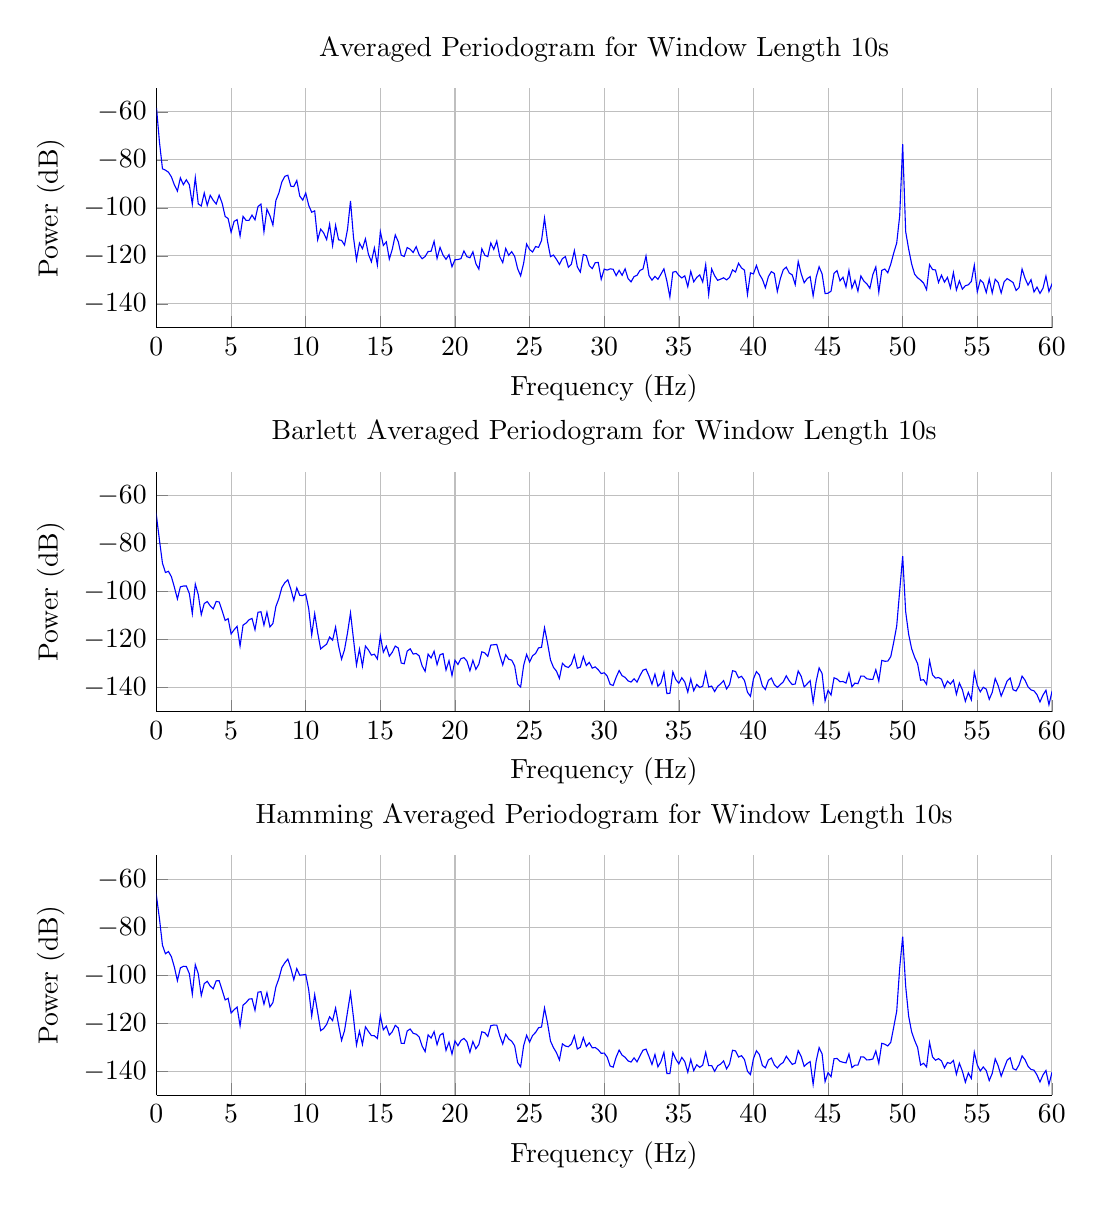
\begin{tikzpicture}

\begin{axis}[%
width=4.47708333333333in,
height=1.2in,
scale only axis,
xmin=0,
xmax=60,
xlabel={Frequency (Hz)},
xmajorgrids,
ymin=-150,
ymax=-50,
ylabel={Power (dB)},
ymajorgrids,
name=plot2,
title={Barlett Averaged Periodogram for Window Length 10s},
axis x line*=bottom,
axis y line*=left
]
\addplot [color=blue,solid,forget plot]
  table[row sep=crcr]{-600	-165.105635140837\\
-599.8	-164.877968944701\\
-599.6	-161.126325969728\\
-599.4	-157.177418290436\\
-599.2	-162.511914296123\\
-599	-162.567498307103\\
-598.8	-156.482440201256\\
-598.6	-158.86435982297\\
-598.4	-164.097624617774\\
-598.2	-168.820420938626\\
-598	-169.99631510102\\
-597.8	-164.723597987451\\
-597.6	-162.343075273531\\
-597.4	-167.435277835148\\
-597.2	-162.465580817443\\
-597	-160.067352780699\\
-596.8	-161.600255877409\\
-596.6	-163.707935573586\\
-596.4	-161.123285633153\\
-596.2	-163.494324959837\\
-596	-162.885760249434\\
-595.8	-158.167005035973\\
-595.6	-165.163814960794\\
-595.4	-164.326687823318\\
-595.2	-160.967622734514\\
-595	-168.309707890921\\
-594.8	-162.308239370721\\
-594.6	-161.810511649913\\
-594.4	-166.589086044509\\
-594.2	-161.474901000333\\
-594	-166.310956214787\\
-593.8	-164.376773316343\\
-593.6	-164.803945469349\\
-593.4	-166.567941640181\\
-593.2	-159.478891405261\\
-593	-158.364343858612\\
-592.8	-166.322343918874\\
-592.6	-168.194227954289\\
-592.4	-162.283339173198\\
-592.2	-158.445873709227\\
-592	-158.744855107714\\
-591.8	-161.560949739737\\
-591.6	-164.51136104101\\
-591.4	-159.883903233059\\
-591.2	-163.477232548669\\
-591	-162.159321816144\\
-590.8	-168.97259672604\\
-590.6	-160.485579842792\\
-590.4	-159.990267221393\\
-590.2	-157.039686326306\\
-590	-165.04585114516\\
-589.8	-165.857522144243\\
-589.6	-165.829835952997\\
-589.4	-167.825064824936\\
-589.2	-167.265846050818\\
-589	-161.416210190162\\
-588.8	-163.972633347769\\
-588.6	-164.347365582245\\
-588.4	-161.020483736368\\
-588.2	-156.259161013273\\
-588	-163.365711773106\\
-587.8	-166.703712268225\\
-587.6	-160.621561120737\\
-587.4	-157.414665942904\\
-587.2	-166.011978630848\\
-587	-159.547109910712\\
-586.8	-162.602289776013\\
-586.6	-164.125973472906\\
-586.4	-162.644559020393\\
-586.2	-161.91127248869\\
-586	-158.52080762322\\
-585.8	-166.024295514263\\
-585.6	-155.039244281372\\
-585.4	-159.526720608986\\
-585.2	-162.821046727676\\
-585	-160.895075209128\\
-584.8	-158.721841323233\\
-584.6	-162.377298923191\\
-584.4	-162.955321472434\\
-584.2	-164.346578813553\\
-584	-163.774311253869\\
-583.8	-164.376418627542\\
-583.6	-161.686074665378\\
-583.4	-163.068399822148\\
-583.2	-159.243389326794\\
-583	-161.943175615006\\
-582.8	-158.051577517207\\
-582.6	-165.547866614333\\
-582.4	-158.933604793657\\
-582.2	-160.582965881099\\
-582	-167.045360646512\\
-581.8	-163.156272754901\\
-581.6	-165.982378677726\\
-581.4	-166.606192958065\\
-581.2	-160.465079879418\\
-581	-158.766387135987\\
-580.8	-164.850326406026\\
-580.6	-166.509731665462\\
-580.4	-160.361682100092\\
-580.2	-167.231549514188\\
-580	-168.142740644578\\
-579.8	-163.266555365165\\
-579.6	-165.318271450022\\
-579.4	-161.45801390994\\
-579.2	-158.368092558986\\
-579	-158.731972743037\\
-578.8	-165.016242898103\\
-578.6	-160.516177003884\\
-578.4	-160.301119316483\\
-578.2	-158.27279411617\\
-578	-165.14952357497\\
-577.8	-163.833180040164\\
-577.6	-162.854455957247\\
-577.4	-166.666591733894\\
-577.2	-159.298855200402\\
-577	-165.594163953828\\
-576.8	-171.197904195582\\
-576.6	-171.728862668669\\
-576.4	-166.528567053157\\
-576.2	-166.270976183319\\
-576	-160.109201541825\\
-575.8	-161.402754065544\\
-575.6	-164.076432536595\\
-575.4	-175.024315105518\\
-575.2	-169.852450321396\\
-575	-155.901493715615\\
-574.8	-162.793295685967\\
-574.6	-165.117447540132\\
-574.4	-165.31914427997\\
-574.2	-164.659763757252\\
-574	-167.859074395226\\
-573.8	-164.544901591408\\
-573.6	-161.451794564926\\
-573.4	-161.495329275776\\
-573.2	-158.559092410843\\
-573	-162.432732414242\\
-572.8	-161.200789741466\\
-572.6	-157.114499456793\\
-572.4	-161.213914455813\\
-572.2	-161.712970962514\\
-572	-158.786516203054\\
-571.8	-157.999913185651\\
-571.6	-160.741374781404\\
-571.4	-160.404800220954\\
-571.2	-163.731819377919\\
-571	-165.52215046486\\
-570.8	-167.109138797552\\
-570.6	-158.688030187026\\
-570.4	-156.47825826747\\
-570.2	-163.690589701912\\
-570	-163.915829704526\\
-569.8	-161.677045313353\\
-569.6	-161.415899235755\\
-569.4	-156.520992133413\\
-569.2	-164.456015698485\\
-569	-159.808591682987\\
-568.8	-161.656167377656\\
-568.6	-160.304546603568\\
-568.4	-159.991765269898\\
-568.2	-159.935348191766\\
-568	-163.704261458103\\
-567.8	-159.336830567122\\
-567.6	-161.02975115981\\
-567.4	-159.595691424885\\
-567.2	-163.300360053833\\
-567	-161.736820990165\\
-566.8	-162.631612255769\\
-566.6	-167.443151063105\\
-566.4	-162.467422503227\\
-566.2	-164.904212530921\\
-566	-161.972777113506\\
-565.8	-160.580608167695\\
-565.6	-162.43470984458\\
-565.4	-158.069866926183\\
-565.2	-157.367270026443\\
-565	-159.503603167028\\
-564.8	-158.626519914467\\
-564.6	-166.041824137348\\
-564.4	-166.260168579958\\
-564.2	-158.537048539602\\
-564	-163.434873948869\\
-563.8	-163.009854964966\\
-563.6	-159.30797799687\\
-563.4	-162.539005873905\\
-563.2	-157.739946118104\\
-563	-168.21975826182\\
-562.8	-164.413852458735\\
-562.6	-166.580669157831\\
-562.4	-159.690843767351\\
-562.2	-160.973710761809\\
-562	-166.73764214155\\
-561.8	-162.366864600658\\
-561.6	-159.51305622765\\
-561.4	-163.266699894342\\
-561.2	-158.904387074517\\
-561	-156.389802176119\\
-560.8	-163.621678133855\\
-560.6	-165.159350815156\\
-560.4	-164.890683496346\\
-560.2	-164.781626775997\\
-560	-164.787669292862\\
-559.8	-163.678566082363\\
-559.6	-161.631167084594\\
-559.4	-161.379104844778\\
-559.2	-167.547953066136\\
-559	-164.542005610692\\
-558.8	-160.216849624072\\
-558.6	-161.738029303252\\
-558.4	-165.020656557527\\
-558.2	-172.603464907472\\
-558	-160.226324424014\\
-557.8	-156.026253305694\\
-557.6	-162.976886750487\\
-557.4	-167.69076802579\\
-557.2	-160.767331391532\\
-557	-158.567659344687\\
-556.8	-159.935245377923\\
-556.6	-163.830819013746\\
-556.4	-162.671432515686\\
-556.2	-162.35686991196\\
-556	-157.13479936193\\
-555.8	-160.168196999159\\
-555.6	-166.182039223811\\
-555.4	-163.483545608539\\
-555.2	-162.818525373064\\
-555	-161.723366823706\\
-554.8	-162.200542186498\\
-554.6	-160.315925554317\\
-554.4	-162.558298543675\\
-554.2	-157.490524705008\\
-554	-161.3695564219\\
-553.8	-165.603826925084\\
-553.6	-160.424892696666\\
-553.4	-158.541757483674\\
-553.2	-160.018240741458\\
-553	-162.053108806813\\
-552.8	-162.730532959696\\
-552.6	-161.851036773149\\
-552.4	-161.310082457033\\
-552.2	-164.332882236991\\
-552	-156.738452325959\\
-551.8	-159.906911597906\\
-551.6	-162.504304651841\\
-551.4	-164.976310204412\\
-551.2	-167.94628043715\\
-551	-163.867834504227\\
-550.8	-159.878204006703\\
-550.6	-150.899224225133\\
-550.4	-147.43775053713\\
-550.2	-149.539502156015\\
-550	-160.137205929695\\
-549.8	-156.475449803272\\
-549.6	-154.459207471063\\
-549.4	-157.874687939144\\
-549.2	-154.55094305557\\
-549	-158.081310700852\\
-548.8	-163.822106217029\\
-548.6	-170.760382334585\\
-548.4	-159.149011134521\\
-548.2	-160.402468200188\\
-548	-163.399573301869\\
-547.8	-165.13215554732\\
-547.6	-159.525851590624\\
-547.4	-161.066310093474\\
-547.2	-162.568752353203\\
-547	-161.18425854048\\
-546.8	-160.060908540105\\
-546.6	-161.086454781004\\
-546.4	-161.679909308784\\
-546.2	-161.935558078569\\
-546	-163.30186220666\\
-545.8	-162.736745315504\\
-545.6	-166.525646870527\\
-545.4	-159.723258954696\\
-545.2	-159.894490484746\\
-545	-160.227045299262\\
-544.8	-163.623371416424\\
-544.6	-161.836475166217\\
-544.4	-159.873072899427\\
-544.2	-156.046493344424\\
-544	-161.048599861014\\
-543.8	-163.973211729227\\
-543.6	-158.868139670571\\
-543.4	-160.517325169321\\
-543.2	-161.129456460371\\
-543	-164.793847145432\\
-542.8	-164.73725083567\\
-542.6	-164.416816300714\\
-542.4	-163.249772557233\\
-542.2	-159.01365192099\\
-542	-161.237597749143\\
-541.8	-162.483702420678\\
-541.6	-161.746027620629\\
-541.4	-160.958089075567\\
-541.2	-164.163075116217\\
-541	-160.629066466146\\
-540.8	-165.106261623386\\
-540.6	-159.951913573438\\
-540.4	-159.634909647721\\
-540.2	-159.486850037641\\
-540	-164.283621303804\\
-539.8	-162.62796493047\\
-539.6	-163.889503711388\\
-539.4	-161.506672114469\\
-539.2	-166.498686834198\\
-539	-161.81217921411\\
-538.8	-157.326150870633\\
-538.6	-159.744564459596\\
-538.4	-164.227500147688\\
-538.2	-162.593920630521\\
-538	-160.484376581168\\
-537.8	-166.922929787183\\
-537.6	-157.775409956093\\
-537.4	-160.846559154646\\
-537.2	-158.741651610063\\
-537	-166.622422740998\\
-536.8	-164.762497052426\\
-536.6	-167.795248811065\\
-536.4	-163.48556660662\\
-536.2	-167.986071751059\\
-536	-163.989334109633\\
-535.8	-164.038424965471\\
-535.6	-159.058764989391\\
-535.4	-159.85437004289\\
-535.2	-166.875310857249\\
-535	-165.511098524294\\
-534.8	-162.142121515592\\
-534.6	-162.186152422004\\
-534.4	-157.546986134239\\
-534.2	-163.30424683176\\
-534	-163.435476041762\\
-533.8	-161.425220563173\\
-533.6	-161.015344623389\\
-533.4	-159.697463956018\\
-533.2	-152.692604812739\\
-533	-155.959625090349\\
-532.8	-158.425299139406\\
-532.6	-157.066965650578\\
-532.4	-164.25991667879\\
-532.2	-154.696619472848\\
-532	-156.58497973587\\
-531.8	-155.461771578111\\
-531.6	-157.058393948313\\
-531.4	-153.860882586976\\
-531.2	-164.249106798771\\
-531	-164.860121495955\\
-530.8	-163.439123991171\\
-530.6	-161.26236261209\\
-530.4	-160.623450623078\\
-530.2	-153.446626270341\\
-530	-161.672656592253\\
-529.8	-161.14917403032\\
-529.6	-155.560900165697\\
-529.4	-159.245983532558\\
-529.2	-163.443429468192\\
-529	-163.183145939119\\
-528.8	-154.65461659539\\
-528.6	-158.54694326458\\
-528.4	-160.570505301479\\
-528.2	-156.565913547117\\
-528	-158.79764594116\\
-527.8	-163.070643363886\\
-527.6	-161.451202890207\\
-527.4	-157.518064296839\\
-527.2	-164.791400554044\\
-527	-166.551215234382\\
-526.8	-161.091016123002\\
-526.6	-162.079459080096\\
-526.4	-163.557931186498\\
-526.2	-159.868553516638\\
-526	-164.526576518783\\
-525.8	-163.679686254795\\
-525.6	-163.177308228357\\
-525.4	-160.950543816033\\
-525.2	-157.800027388594\\
-525	-162.429305931698\\
-524.8	-161.348426707707\\
-524.6	-158.233681996485\\
-524.4	-157.077305024836\\
-524.2	-163.949931151807\\
-524	-162.473888995621\\
-523.8	-163.502873889935\\
-523.6	-165.917433341004\\
-523.4	-171.243029637625\\
-523.2	-158.947030257039\\
-523	-163.975062024237\\
-522.8	-166.598900216221\\
-522.6	-164.340913547419\\
-522.4	-164.296349139086\\
-522.2	-159.259208897653\\
-522	-160.065813195481\\
-521.8	-157.758081330072\\
-521.6	-156.881139270179\\
-521.4	-156.687518679544\\
-521.2	-161.85392980441\\
-521	-161.693085787888\\
-520.8	-161.318184824294\\
-520.6	-164.868449936784\\
-520.4	-165.968263088374\\
-520.2	-165.39013816382\\
-520	-161.274195871577\\
-519.8	-158.951449292539\\
-519.6	-156.982365342581\\
-519.4	-163.775771750051\\
-519.2	-164.535438255509\\
-519	-161.727981262838\\
-518.8	-163.983539648497\\
-518.6	-161.996602570322\\
-518.4	-159.221053895\\
-518.2	-161.297531110331\\
-518	-158.079313131692\\
-517.8	-161.341916147558\\
-517.6	-163.874367998578\\
-517.4	-166.763805893451\\
-517.2	-160.418685037699\\
-517	-159.549123175377\\
-516.8	-168.389774711497\\
-516.6	-161.837766175046\\
-516.4	-167.324000670417\\
-516.2	-163.018258166275\\
-516	-160.13261977139\\
-515.8	-161.495086891062\\
-515.6	-169.188448182449\\
-515.4	-158.583247833339\\
-515.2	-154.206794221222\\
-515	-161.715721202588\\
-514.8	-159.68791205079\\
-514.6	-158.738028744527\\
-514.4	-157.739252787453\\
-514.2	-160.373000663848\\
-514	-159.775116651496\\
-513.8	-163.074970504441\\
-513.6	-159.009550233066\\
-513.4	-156.808727071471\\
-513.2	-154.885818504481\\
-513	-162.012514224459\\
-512.8	-159.705366462905\\
-512.6	-157.472959919105\\
-512.4	-165.729739652591\\
-512.2	-158.800021788968\\
-512	-156.862123403157\\
-511.8	-159.138308109431\\
-511.6	-166.377260355739\\
-511.4	-169.048565037298\\
-511.2	-164.079343336358\\
-511	-161.701229783436\\
-510.8	-168.64494314974\\
-510.6	-157.522963555528\\
-510.4	-165.150566073615\\
-510.2	-164.655687530084\\
-510	-164.203611523205\\
-509.8	-161.721062674997\\
-509.6	-159.691238361501\\
-509.4	-160.910491626047\\
-509.2	-163.430096652479\\
-509	-161.432012393321\\
-508.8	-160.123363366399\\
-508.6	-159.34224435644\\
-508.4	-159.1241860168\\
-508.2	-155.894956184852\\
-508	-155.658322666315\\
-507.8	-159.638725354813\\
-507.6	-165.778260032483\\
-507.4	-159.021537446753\\
-507.2	-158.647944879492\\
-507	-158.170656345621\\
-506.8	-158.965017824054\\
-506.6	-158.778887924379\\
-506.4	-157.746616838479\\
-506.2	-156.543278645235\\
-506	-161.252817148653\\
-505.8	-162.118682062818\\
-505.6	-163.030639496258\\
-505.4	-163.158087024807\\
-505.2	-159.864408338417\\
-505	-155.321512187858\\
-504.8	-159.668689859872\\
-504.6	-161.443238156155\\
-504.4	-165.982147302534\\
-504.2	-159.380393657945\\
-504	-163.572332311159\\
-503.8	-154.249555684547\\
-503.6	-153.072924705483\\
-503.4	-157.253856450905\\
-503.2	-163.52607557066\\
-503	-159.869798111576\\
-502.8	-162.82538369396\\
-502.6	-162.443761418255\\
-502.4	-158.273526153617\\
-502.2	-160.824021163005\\
-502	-165.598473533742\\
-501.8	-159.94502108827\\
-501.6	-159.828158177409\\
-501.4	-164.424359532382\\
-501.2	-159.605603135625\\
-501	-156.406085305815\\
-500.8	-158.519760332739\\
-500.6	-158.379777225136\\
-500.4	-158.488526050559\\
-500.2	-157.853069915742\\
-500	-161.595528901204\\
-499.8	-160.743668368759\\
-499.6	-159.086095675871\\
-499.4	-160.369686118205\\
-499.2	-158.111794794056\\
-499	-159.861308018132\\
-498.8	-156.339091858923\\
-498.6	-162.976469483813\\
-498.4	-163.78366947429\\
-498.2	-161.287742805287\\
-498	-164.477145784577\\
-497.8	-160.83094574445\\
-497.6	-163.412667266177\\
-497.4	-160.118175833564\\
-497.2	-159.04753681816\\
-497	-158.372314618171\\
-496.8	-166.568502326041\\
-496.6	-161.435950865193\\
-496.4	-158.968720533031\\
-496.2	-162.909871947308\\
-496	-159.041856859264\\
-495.8	-160.186469949896\\
-495.6	-160.982693549947\\
-495.4	-167.046501567407\\
-495.2	-163.309443897084\\
-495	-161.638905341207\\
-494.8	-159.714413590179\\
-494.6	-159.01500969529\\
-494.4	-162.61596113447\\
-494.2	-164.06236102328\\
-494	-163.188119815553\\
-493.8	-157.65691028488\\
-493.6	-161.841489976572\\
-493.4	-158.216812865056\\
-493.2	-159.206273391213\\
-493	-156.356901847826\\
-492.8	-157.718092936156\\
-492.6	-159.535708826466\\
-492.4	-165.449291991849\\
-492.2	-157.177202473057\\
-492	-157.456286142749\\
-491.8	-157.193149490274\\
-491.6	-160.063264788524\\
-491.4	-161.355752144269\\
-491.2	-163.324975031306\\
-491	-160.812103423537\\
-490.8	-164.361027322044\\
-490.6	-158.975625096895\\
-490.4	-162.273842334028\\
-490.2	-163.065290019559\\
-490	-162.411415742524\\
-489.8	-155.353164002861\\
-489.6	-161.4868330078\\
-489.4	-159.328279455546\\
-489.2	-160.457252879691\\
-489	-162.50271271822\\
-488.8	-162.055470108583\\
-488.6	-163.718987550305\\
-488.4	-158.779396144819\\
-488.2	-160.538508003082\\
-488	-153.93560282652\\
-487.8	-157.085626565774\\
-487.6	-161.665318244582\\
-487.4	-160.92930361705\\
-487.2	-159.109786933221\\
-487	-158.900134485795\\
-486.8	-161.787838428553\\
-486.6	-157.152061206563\\
-486.4	-165.027594508563\\
-486.2	-166.497739602755\\
-486	-163.072859384602\\
-485.8	-165.840447634724\\
-485.6	-157.410849464\\
-485.4	-157.101212569952\\
-485.2	-163.549819018231\\
-485	-161.291157725369\\
-484.8	-163.9104630703\\
-484.6	-163.537311667053\\
-484.4	-159.284407491032\\
-484.2	-165.026392135142\\
-484	-158.253255567403\\
-483.8	-158.447727450953\\
-483.6	-164.011469819557\\
-483.4	-157.884210390706\\
-483.2	-159.115548633462\\
-483	-152.60455847191\\
-482.8	-157.166448744483\\
-482.6	-156.462646660173\\
-482.4	-154.01159079785\\
-482.2	-154.247696625071\\
-482	-162.296666773206\\
-481.8	-156.977664904479\\
-481.6	-160.537088658056\\
-481.4	-156.176952401121\\
-481.2	-156.817935464035\\
-481	-166.925639162854\\
-480.8	-161.347197874709\\
-480.6	-155.879570750798\\
-480.4	-167.307245004842\\
-480.2	-160.723699414178\\
-480	-162.932108724765\\
-479.8	-160.092939390795\\
-479.6	-158.195505292583\\
-479.4	-158.1535108228\\
-479.2	-156.381115376722\\
-479	-158.970500063111\\
-478.8	-165.60352838816\\
-478.6	-166.548192312657\\
-478.4	-158.980602428405\\
-478.2	-160.314501593631\\
-478	-159.485850905082\\
-477.8	-157.919902117481\\
-477.6	-158.501053176006\\
-477.4	-159.428345743262\\
-477.2	-160.98451973694\\
-477	-163.463931907629\\
-476.8	-159.453026612832\\
-476.6	-158.092690649608\\
-476.4	-158.570482708319\\
-476.2	-156.473914583035\\
-476	-158.103499488265\\
-475.8	-161.439937446462\\
-475.6	-160.308471090973\\
-475.4	-158.095041494066\\
-475.2	-163.52426847964\\
-475	-157.609200128152\\
-474.8	-153.526475763007\\
-474.6	-155.436240039154\\
-474.4	-157.719021486387\\
-474.2	-161.025623377455\\
-474	-158.976189286522\\
-473.8	-157.504199234882\\
-473.6	-163.440267583431\\
-473.4	-157.162162331239\\
-473.2	-162.107046528924\\
-473	-153.650883727175\\
-472.8	-152.920061819946\\
-472.6	-159.418692626919\\
-472.4	-159.532216896757\\
-472.2	-157.880420179589\\
-472	-157.746213239579\\
-471.8	-160.176537027891\\
-471.6	-161.963457505336\\
-471.4	-157.037471554435\\
-471.2	-160.791317957183\\
-471	-160.13604105406\\
-470.8	-158.075302285349\\
-470.6	-161.476180816227\\
-470.4	-161.402751520778\\
-470.2	-160.040207092006\\
-470	-162.931277109953\\
-469.8	-158.651201777541\\
-469.6	-159.735653968538\\
-469.4	-159.803679917626\\
-469.2	-163.940500976621\\
-469	-161.86446129091\\
-468.8	-156.319816541893\\
-468.6	-161.452040933947\\
-468.4	-160.397779653701\\
-468.2	-161.695944810249\\
-468	-162.205043720088\\
-467.8	-160.681630425126\\
-467.6	-155.300524257573\\
-467.4	-157.829776663628\\
-467.2	-162.840718314444\\
-467	-162.670227422799\\
-466.8	-158.23309819665\\
-466.6	-159.53808664928\\
-466.4	-156.796529581597\\
-466.2	-158.617426132728\\
-466	-158.130797403184\\
-465.8	-158.329374084289\\
-465.6	-157.193435596171\\
-465.4	-155.463048759038\\
-465.2	-154.876107079231\\
-465	-156.167059399749\\
-464.8	-162.382678850456\\
-464.6	-161.521581377989\\
-464.4	-161.885786669347\\
-464.2	-157.90807284107\\
-464	-161.818474523219\\
-463.8	-160.360511573466\\
-463.6	-159.770896962203\\
-463.4	-158.128700026323\\
-463.2	-155.619349877569\\
-463	-155.819019338736\\
-462.8	-160.945874524611\\
-462.6	-168.880208889337\\
-462.4	-160.448417816278\\
-462.2	-152.334317802939\\
-462	-150.421463920657\\
-461.8	-161.590455421695\\
-461.6	-162.825099877316\\
-461.4	-164.753449791783\\
-461.2	-159.028948509838\\
-461	-159.330118349394\\
-460.8	-162.439332677099\\
-460.6	-167.864852905586\\
-460.4	-160.648425388896\\
-460.2	-159.40455570097\\
-460	-156.546800180904\\
-459.8	-161.498493076757\\
-459.6	-160.180351728661\\
-459.4	-160.201217332168\\
-459.2	-161.896293910685\\
-459	-159.555328983867\\
-458.8	-161.289710871343\\
-458.6	-162.058765648116\\
-458.4	-165.553883803482\\
-458.2	-160.607041858813\\
-458	-159.51193360394\\
-457.8	-161.975520102261\\
-457.6	-156.76068176372\\
-457.4	-158.883728734714\\
-457.2	-157.121726173746\\
-457	-163.416746209021\\
-456.8	-164.61494308498\\
-456.6	-163.516799187317\\
-456.4	-158.458917492151\\
-456.2	-158.161538003605\\
-456	-158.260725454235\\
-455.8	-158.831640898996\\
-455.6	-154.918386105411\\
-455.4	-162.026554680303\\
-455.2	-159.520577041779\\
-455	-162.335148375803\\
-454.8	-163.074556929348\\
-454.6	-163.452599466219\\
-454.4	-158.875319750197\\
-454.2	-155.069752269376\\
-454	-158.541829756612\\
-453.8	-160.872971824976\\
-453.6	-159.671259559644\\
-453.4	-159.801094252208\\
-453.2	-163.473189359361\\
-453	-160.821901067662\\
-452.8	-158.38082702843\\
-452.6	-158.064829408433\\
-452.4	-159.567768641112\\
-452.2	-162.181458043266\\
-452	-161.257548422943\\
-451.8	-161.015596012183\\
-451.6	-158.648051295709\\
-451.4	-157.846141677408\\
-451.2	-159.404181500568\\
-451	-157.188915064462\\
-450.8	-163.470334864282\\
-450.6	-163.240242722132\\
-450.4	-155.456272859112\\
-450.2	-154.78180694771\\
-450	-159.538286578457\\
-449.8	-149.755494048559\\
-449.6	-150.306861413404\\
-449.4	-157.746298569721\\
-449.2	-158.635702349679\\
-449	-159.153779178775\\
-448.8	-159.122789095955\\
-448.6	-155.463989090697\\
-448.4	-160.30512087025\\
-448.2	-161.847120187688\\
-448	-160.33235154076\\
-447.8	-157.674028303633\\
-447.6	-157.221483321363\\
-447.4	-157.155692379099\\
-447.2	-155.381244769049\\
-447	-153.270703444611\\
-446.8	-155.299389530977\\
-446.6	-155.203630147741\\
-446.4	-155.632724507093\\
-446.2	-158.029399775168\\
-446	-155.991530707542\\
-445.8	-162.884044893411\\
-445.6	-156.799257604907\\
-445.4	-157.828251865959\\
-445.2	-154.87322059344\\
-445	-157.933786695849\\
-444.8	-158.148330815201\\
-444.6	-154.088640376901\\
-444.4	-154.964048095077\\
-444.2	-162.614481780804\\
-444	-155.84620466817\\
-443.8	-160.172876174613\\
-443.6	-161.158998075259\\
-443.4	-158.854337163534\\
-443.2	-159.575948079822\\
-443	-157.551812146024\\
-442.8	-158.348169473476\\
-442.6	-158.942079057096\\
-442.4	-158.915639933335\\
-442.2	-153.206259156612\\
-442	-157.072712890799\\
-441.8	-157.709458711215\\
-441.6	-161.844113901054\\
-441.4	-162.836805569163\\
-441.2	-155.676738863298\\
-441	-155.476300426512\\
-440.8	-160.107426158563\\
-440.6	-158.623501286129\\
-440.4	-160.043560005944\\
-440.2	-156.547441617817\\
-440	-159.656030025447\\
-439.8	-159.2108717066\\
-439.6	-158.598041819524\\
-439.4	-171.909140035433\\
-439.2	-159.758428804586\\
-439	-163.631687898056\\
-438.8	-167.398011389134\\
-438.6	-163.246860243481\\
-438.4	-158.773230235652\\
-438.2	-157.456915857198\\
-438	-161.549458001782\\
-437.8	-154.281902241338\\
-437.6	-155.876526255713\\
-437.4	-157.705596372595\\
-437.2	-152.306256465191\\
-437	-156.643887370075\\
-436.8	-155.542501105971\\
-436.6	-151.862700255232\\
-436.4	-158.647998522193\\
-436.2	-160.762403169759\\
-436	-155.780804835191\\
-435.8	-158.350894390517\\
-435.6	-160.565996039631\\
-435.4	-155.414820073793\\
-435.2	-154.862622373322\\
-435	-161.580327726927\\
-434.8	-159.861132817585\\
-434.6	-156.21984828366\\
-434.4	-163.844981351264\\
-434.2	-155.368451252772\\
-434	-153.718965720456\\
-433.8	-158.839194176285\\
-433.6	-157.228380224628\\
-433.4	-153.119631317279\\
-433.2	-161.709192745874\\
-433	-158.626302556927\\
-432.8	-158.692643831118\\
-432.6	-165.70587019378\\
-432.4	-159.222819886444\\
-432.2	-164.203630252568\\
-432	-157.250827992693\\
-431.8	-161.684865173798\\
-431.6	-165.106261226702\\
-431.4	-162.264076998859\\
-431.2	-158.481652421128\\
-431	-152.397425745338\\
-430.8	-157.627972878088\\
-430.6	-157.439064915468\\
-430.4	-158.882267735686\\
-430.2	-157.56639017572\\
-430	-157.01844477438\\
-429.8	-155.567425585473\\
-429.6	-161.374100236897\\
-429.4	-156.258277494178\\
-429.2	-156.856105486221\\
-429	-161.226356032627\\
-428.8	-154.846390170031\\
-428.6	-155.611998295244\\
-428.4	-163.140741140914\\
-428.2	-150.411682719184\\
-428	-155.24198140696\\
-427.8	-156.278464729147\\
-427.6	-153.410894360751\\
-427.4	-156.760349610479\\
-427.2	-157.159298821636\\
-427	-160.839085678155\\
-426.8	-156.610046289043\\
-426.6	-159.41949749504\\
-426.4	-159.52830040428\\
-426.2	-160.299731104649\\
-426	-158.483330377929\\
-425.8	-151.579120611328\\
-425.6	-152.046541673209\\
-425.4	-160.2311921001\\
-425.2	-166.213256490787\\
-425	-154.349346176108\\
-424.8	-153.649746186425\\
-424.6	-158.871613563195\\
-424.4	-156.084313154783\\
-424.2	-157.483720385114\\
-424	-158.573233093933\\
-423.8	-162.210555385978\\
-423.6	-157.718729383455\\
-423.4	-161.796931115205\\
-423.2	-158.435143349126\\
-423	-154.073950353152\\
-422.8	-157.161359134963\\
-422.6	-158.860378373431\\
-422.4	-156.870701464262\\
-422.2	-163.476484409354\\
-422	-165.590185840059\\
-421.8	-161.881525072872\\
-421.6	-158.40493448656\\
-421.4	-162.188444553938\\
-421.2	-157.50061144347\\
-421	-155.195294138417\\
-420.8	-157.206967776899\\
-420.6	-161.069552974869\\
-420.4	-158.292402092683\\
-420.2	-159.128192330905\\
-420	-160.939641331313\\
-419.8	-165.765334295545\\
-419.6	-165.506404989295\\
-419.4	-155.674941389163\\
-419.2	-159.509394227534\\
-419	-165.773071893006\\
-418.8	-159.726496341365\\
-418.6	-159.686138747163\\
-418.4	-158.830436810408\\
-418.2	-153.77272325445\\
-418	-156.939267843827\\
-417.8	-156.928909138154\\
-417.6	-162.384927443703\\
-417.4	-159.326409104377\\
-417.2	-155.480683692504\\
-417	-158.34545733058\\
-416.8	-157.890320741829\\
-416.6	-154.880505701238\\
-416.4	-157.749845518863\\
-416.2	-155.922065859292\\
-416	-157.726866172582\\
-415.8	-162.456261313071\\
-415.6	-156.812767771372\\
-415.4	-151.419351568048\\
-415.2	-153.227557710435\\
-415	-159.184755791221\\
-414.8	-156.7113278713\\
-414.6	-158.524215001081\\
-414.4	-153.836718732085\\
-414.2	-153.868553262039\\
-414	-155.672712048591\\
-413.8	-160.696040594591\\
-413.6	-158.617953514849\\
-413.4	-151.183021369893\\
-413.2	-160.980633331886\\
-413	-156.804436608226\\
-412.8	-159.833209613466\\
-412.6	-162.625207207458\\
-412.4	-159.140693632435\\
-412.2	-155.22687333578\\
-412	-160.03290751594\\
-411.8	-156.407097845807\\
-411.6	-151.4456328323\\
-411.4	-154.420774156472\\
-411.2	-153.014774898939\\
-411	-156.246927550809\\
-410.8	-157.732702704011\\
-410.6	-156.778674295484\\
-410.4	-156.294430940997\\
-410.2	-153.468216813596\\
-410	-163.411627596369\\
-409.8	-155.109616347422\\
-409.6	-158.036620653513\\
-409.4	-154.419536787362\\
-409.2	-155.603747411348\\
-409	-154.367800841049\\
-408.8	-154.452229506089\\
-408.6	-157.141230779037\\
-408.4	-160.319854157905\\
-408.2	-157.51707576204\\
-408	-158.92568844899\\
-407.8	-158.302707628624\\
-407.6	-155.573589774423\\
-407.4	-162.074703624522\\
-407.2	-160.615049911072\\
-407	-159.411953514803\\
-406.8	-157.438066610621\\
-406.6	-155.518522114896\\
-406.4	-160.327222333353\\
-406.2	-163.210690780937\\
-406	-157.100097751338\\
-405.8	-156.431634146161\\
-405.6	-158.474387363742\\
-405.4	-159.444347577587\\
-405.2	-162.957972619054\\
-405	-157.619621885975\\
-404.8	-152.91937893249\\
-404.6	-154.783183560098\\
-404.4	-154.01641923187\\
-404.2	-150.952185417175\\
-404	-149.794797545952\\
-403.8	-156.420077625253\\
-403.6	-158.200634212273\\
-403.4	-152.396378198252\\
-403.2	-156.835532861886\\
-403	-156.824752176454\\
-402.8	-157.845022465096\\
-402.6	-156.883501605771\\
-402.4	-162.730754135004\\
-402.2	-162.301637987973\\
-402	-161.219406015403\\
-401.8	-155.83967052762\\
-401.6	-160.152627314228\\
-401.4	-160.670815741275\\
-401.2	-158.570757718493\\
-401	-154.966587805119\\
-400.8	-155.074715021666\\
-400.6	-155.546094003878\\
-400.4	-155.729513976636\\
-400.2	-158.065778234096\\
-400	-157.934550974564\\
-399.8	-164.966357616138\\
-399.6	-156.094534721104\\
-399.4	-154.072303150856\\
-399.2	-154.073010585769\\
-399	-157.468008717651\\
-398.8	-160.219869783354\\
-398.6	-164.987265757235\\
-398.4	-158.773506075204\\
-398.2	-159.658272147399\\
-398	-152.907815696339\\
-397.8	-153.575173620165\\
-397.6	-161.939065453664\\
-397.4	-154.795269692969\\
-397.2	-155.336015052764\\
-397	-155.03884496147\\
-396.8	-159.065927082118\\
-396.6	-159.983389136327\\
-396.4	-158.556702003861\\
-396.2	-160.835299437323\\
-396	-157.028769561203\\
-395.8	-160.5247982101\\
-395.6	-158.518975881051\\
-395.4	-162.497263672502\\
-395.2	-159.614677721284\\
-395	-156.110336560214\\
-394.8	-157.014706580342\\
-394.6	-157.108544604438\\
-394.4	-154.939973679772\\
-394.2	-154.083021751791\\
-394	-158.09073465515\\
-393.8	-154.483294135138\\
-393.6	-148.82562947402\\
-393.4	-158.010728880365\\
-393.2	-154.141346613773\\
-393	-151.281081477077\\
-392.8	-149.381867880078\\
-392.6	-152.458090576953\\
-392.4	-157.375358805836\\
-392.2	-156.51094806454\\
-392	-160.67748527911\\
-391.8	-156.183095843126\\
-391.6	-161.423064033399\\
-391.4	-153.90212304741\\
-391.2	-150.96998692263\\
-391	-154.644608989697\\
-390.8	-157.455817320256\\
-390.6	-155.104765344397\\
-390.4	-152.214902147858\\
-390.2	-157.61420434646\\
-390	-164.147961624545\\
-389.8	-157.326773760261\\
-389.6	-153.544608387289\\
-389.4	-154.378561063479\\
-389.2	-153.627375978966\\
-389	-156.870828520807\\
-388.8	-161.516104543334\\
-388.6	-151.225750767854\\
-388.4	-152.979495010705\\
-388.2	-155.995946135772\\
-388	-162.349830918694\\
-387.8	-157.399974459838\\
-387.6	-159.0845422285\\
-387.4	-158.211134778507\\
-387.2	-155.307280765841\\
-387	-155.987581596313\\
-386.8	-162.854060328851\\
-386.6	-158.85910937406\\
-386.4	-161.435396015148\\
-386.2	-156.488653888438\\
-386	-152.702865831024\\
-385.8	-151.146135193891\\
-385.6	-155.231436452603\\
-385.4	-153.296267668494\\
-385.2	-152.779780654334\\
-385	-157.606823528534\\
-384.8	-156.240369042223\\
-384.6	-156.75862911967\\
-384.4	-158.509981925059\\
-384.2	-156.93564480128\\
-384	-155.224149917534\\
-383.8	-156.205504417231\\
-383.6	-158.063877010045\\
-383.4	-158.129558426287\\
-383.2	-160.227148331919\\
-383	-156.062842678671\\
-382.8	-152.923796497721\\
-382.6	-159.308993450712\\
-382.4	-159.741524754356\\
-382.2	-155.550909158006\\
-382	-156.558056397637\\
-381.8	-154.769418993558\\
-381.6	-156.844732818376\\
-381.4	-156.553958640007\\
-381.2	-153.143061737259\\
-381	-152.567200809642\\
-380.8	-153.197794982076\\
-380.6	-152.045661864068\\
-380.4	-158.713683887766\\
-380.2	-160.412266662198\\
-380	-156.299302083615\\
-379.8	-155.767599656027\\
-379.6	-157.586563109174\\
-379.4	-152.145175017958\\
-379.2	-152.987801375789\\
-379	-157.159654942645\\
-378.8	-157.926058323616\\
-378.6	-153.996644363242\\
-378.4	-154.445365750005\\
-378.2	-152.350096987816\\
-378	-155.079159512064\\
-377.8	-154.736813083702\\
-377.6	-152.292714935657\\
-377.4	-155.91975774221\\
-377.2	-157.594909198555\\
-377	-158.087139741507\\
-376.8	-155.65992767954\\
-376.6	-154.946944368304\\
-376.4	-154.515571483896\\
-376.2	-152.890841664555\\
-376	-156.017481802602\\
-375.8	-156.085011643416\\
-375.6	-156.574893566717\\
-375.4	-154.12075509419\\
-375.2	-154.570591027938\\
-375	-154.657908162895\\
-374.8	-156.732511813807\\
-374.6	-153.624250167437\\
-374.4	-158.539897564823\\
-374.2	-158.40653510715\\
-374	-155.005334846463\\
-373.8	-156.682994002388\\
-373.6	-159.244777282627\\
-373.4	-155.925705700344\\
-373.2	-152.351737936319\\
-373	-153.836404560091\\
-372.8	-154.121578876966\\
-372.6	-155.114941839243\\
-372.4	-151.995215827033\\
-372.2	-149.856848635381\\
-372	-149.086481301417\\
-371.8	-152.789342257758\\
-371.6	-155.286763559775\\
-371.4	-150.482137651452\\
-371.2	-158.024167976824\\
-371	-159.302851957572\\
-370.8	-166.623540333626\\
-370.6	-158.289222982863\\
-370.4	-156.712460378454\\
-370.2	-157.72094036663\\
-370	-154.225302663019\\
-369.8	-153.13119299449\\
-369.6	-150.095544960144\\
-369.4	-147.606838040338\\
-369.2	-146.191278508493\\
-369	-145.78828552024\\
-368.8	-149.854655911431\\
-368.6	-156.636548277112\\
-368.4	-151.833619715767\\
-368.2	-153.735968925784\\
-368	-150.760068802116\\
-367.8	-155.204145040355\\
-367.6	-153.030503025729\\
-367.4	-151.262406802395\\
-367.2	-155.847929976497\\
-367	-158.045210514122\\
-366.8	-152.879126614727\\
-366.6	-153.229785510559\\
-366.4	-155.249479192831\\
-366.2	-160.351575522839\\
-366	-151.632737229117\\
-365.8	-154.031504531328\\
-365.6	-153.401016471868\\
-365.4	-156.456847109487\\
-365.2	-154.832159637543\\
-365	-157.276090165083\\
-364.8	-156.642217035264\\
-364.6	-158.829164284368\\
-364.4	-156.017700415784\\
-364.2	-150.491241818319\\
-364	-153.820389932022\\
-363.8	-153.856146850273\\
-363.6	-148.570219503048\\
-363.4	-153.313989711181\\
-363.2	-156.647423057078\\
-363	-154.483735950003\\
-362.8	-155.981482184434\\
-362.6	-150.279145576812\\
-362.4	-158.653470927672\\
-362.2	-158.313781002088\\
-362	-153.339364987061\\
-361.8	-159.573486648458\\
-361.6	-156.048030988081\\
-361.4	-156.761159104843\\
-361.2	-151.010682628242\\
-361	-150.139369360896\\
-360.8	-155.382847376338\\
-360.6	-161.596409862073\\
-360.4	-153.019015592198\\
-360.2	-154.550844559462\\
-360	-153.376943266814\\
-359.8	-158.563711067909\\
-359.6	-152.943860244092\\
-359.4	-149.891426927436\\
-359.2	-157.826589879126\\
-359	-152.690497872085\\
-358.8	-158.050320163702\\
-358.6	-160.173022711423\\
-358.4	-155.486589584861\\
-358.2	-158.137983527479\\
-358	-157.747992090318\\
-357.8	-157.772386314769\\
-357.6	-156.86013169418\\
-357.4	-155.171644614882\\
-357.2	-153.696837772946\\
-357	-156.490222892561\\
-356.8	-154.748374685029\\
-356.6	-155.430955744923\\
-356.4	-159.907745130059\\
-356.2	-158.141571581541\\
-356	-158.166411219898\\
-355.8	-154.139090546758\\
-355.6	-153.690824357652\\
-355.4	-149.759903100215\\
-355.2	-147.898290330778\\
-355	-150.630252438112\\
-354.8	-156.929858666992\\
-354.6	-153.210260697117\\
-354.4	-155.227303826374\\
-354.2	-152.257146322338\\
-354	-154.584972344571\\
-353.8	-156.775965573058\\
-353.6	-151.181115161552\\
-353.4	-151.593952067856\\
-353.2	-153.736751801557\\
-353	-155.574740676001\\
-352.8	-159.681334953969\\
-352.6	-155.117844025448\\
-352.4	-157.181275227773\\
-352.2	-153.89556060486\\
-352	-151.838251432566\\
-351.8	-156.062453397956\\
-351.6	-147.992770010582\\
-351.4	-151.214058051752\\
-351.2	-153.756808637398\\
-351	-159.064207989933\\
-350.8	-156.060138298308\\
-350.6	-153.658035763546\\
-350.4	-153.637216563854\\
-350.2	-152.249270840783\\
-350	-148.50550994232\\
-349.8	-146.733829760019\\
-349.6	-149.386605295816\\
-349.4	-157.574369298128\\
-349.2	-152.851546660297\\
-349	-153.400934109279\\
-348.8	-156.005349691626\\
-348.6	-155.360891634708\\
-348.4	-151.110488847081\\
-348.2	-152.010647552866\\
-348	-155.937444900552\\
-347.8	-159.814548936538\\
-347.6	-161.57842287023\\
-347.4	-151.944578869727\\
-347.2	-150.596568203736\\
-347	-155.027039408525\\
-346.8	-152.35455197903\\
-346.6	-158.91972198643\\
-346.4	-155.667675468132\\
-346.2	-154.702536480646\\
-346	-154.783449857812\\
-345.8	-151.206124905999\\
-345.6	-154.772977205259\\
-345.4	-155.107026411822\\
-345.2	-161.171683379618\\
-345	-157.812466883027\\
-344.8	-153.403562088943\\
-344.6	-155.581928259458\\
-344.4	-158.004794558716\\
-344.2	-158.177697109782\\
-344	-158.902794523928\\
-343.8	-157.856091083348\\
-343.6	-158.361389989384\\
-343.4	-153.934689730576\\
-343.2	-153.31967185587\\
-343	-157.039209959892\\
-342.8	-153.578518547698\\
-342.6	-160.76408982216\\
-342.4	-148.231440960153\\
-342.2	-147.661774179716\\
-342	-147.106946633738\\
-341.8	-150.058627666226\\
-341.6	-150.247562365464\\
-341.4	-158.276366056644\\
-341.2	-161.874590706119\\
-341	-158.174110392403\\
-340.8	-154.679816241018\\
-340.6	-152.299759493278\\
-340.4	-157.052621606975\\
-340.2	-157.220187792987\\
-340	-155.62588974112\\
-339.8	-166.891622762713\\
-339.6	-155.210597280847\\
-339.4	-151.456804000966\\
-339.2	-156.992679021043\\
-339	-154.751634974092\\
-338.8	-153.155186823079\\
-338.6	-153.031954610706\\
-338.4	-156.409743218042\\
-338.2	-155.489026004157\\
-338	-155.939977074725\\
-337.8	-149.885639471123\\
-337.6	-146.567768151179\\
-337.4	-147.494040024674\\
-337.2	-145.408744309267\\
-337	-151.304463706418\\
-336.8	-156.053795713476\\
-336.6	-154.533568342571\\
-336.4	-158.338547178968\\
-336.2	-155.097247961202\\
-336	-159.078765646175\\
-335.8	-158.100583607239\\
-335.6	-150.860971686397\\
-335.4	-151.508692550063\\
-335.2	-151.350960055647\\
-335	-156.817641023156\\
-334.8	-156.387860446576\\
-334.6	-153.152732446924\\
-334.4	-153.850258515544\\
-334.2	-152.83601516937\\
-334	-155.906599743446\\
-333.8	-159.206493392225\\
-333.6	-155.981999945147\\
-333.4	-155.576127118853\\
-333.2	-151.685115496357\\
-333	-154.537519410374\\
-332.8	-152.301158076144\\
-332.6	-154.027033059904\\
-332.4	-149.130657172935\\
-332.2	-156.481131055309\\
-332	-157.554516056564\\
-331.8	-155.582811335999\\
-331.6	-153.465326320068\\
-331.4	-151.988817692588\\
-331.2	-153.960551998894\\
-331	-152.670750648726\\
-330.8	-156.854382587053\\
-330.6	-153.303859629773\\
-330.4	-156.302682286217\\
-330.2	-154.999554503763\\
-330	-155.366443747566\\
-329.8	-156.237786230615\\
-329.6	-156.102566129366\\
-329.4	-159.606796219103\\
-329.2	-156.583762535259\\
-329	-155.899250396659\\
-328.8	-154.963317308664\\
-328.6	-156.250254121575\\
-328.4	-160.209712381461\\
-328.2	-149.785855445547\\
-328	-157.969746538037\\
-327.8	-157.980786073923\\
-327.6	-160.327843249722\\
-327.4	-152.330647379067\\
-327.2	-151.157769766095\\
-327	-154.299701366468\\
-326.8	-163.038921937418\\
-326.6	-155.669626956296\\
-326.4	-153.852173411773\\
-326.2	-153.307615598561\\
-326	-149.916672443899\\
-325.8	-149.69080621089\\
-325.6	-151.464771211564\\
-325.4	-151.791810557357\\
-325.2	-151.69507225591\\
-325	-153.614305184592\\
-324.8	-152.287934702795\\
-324.6	-154.25244042126\\
-324.4	-150.313892913002\\
-324.2	-153.455657852881\\
-324	-150.437039033983\\
-323.8	-151.3350595876\\
-323.6	-159.57540668268\\
-323.4	-149.587927241426\\
-323.2	-148.829285302259\\
-323	-151.371219837464\\
-322.8	-155.005047211826\\
-322.6	-153.28422034372\\
-322.4	-154.554791520675\\
-322.2	-149.130659669738\\
-322	-154.036426346737\\
-321.8	-157.90170392328\\
-321.6	-154.024388983524\\
-321.4	-149.448538324007\\
-321.2	-155.19707482521\\
-321	-149.558221027305\\
-320.8	-152.567286115806\\
-320.6	-158.108039073065\\
-320.4	-158.647228390023\\
-320.2	-151.250545329146\\
-320	-153.461748973641\\
-319.8	-159.27077618422\\
-319.6	-155.389441578695\\
-319.4	-153.246844247485\\
-319.2	-155.956153029204\\
-319	-155.649364499303\\
-318.8	-162.678028182293\\
-318.6	-152.672274544195\\
-318.4	-155.392986538379\\
-318.2	-156.626596438847\\
-318	-155.227194132471\\
-317.8	-152.302661413298\\
-317.6	-155.776474065981\\
-317.4	-157.690591956538\\
-317.2	-156.713565016479\\
-317	-152.818638093399\\
-316.8	-153.122478983086\\
-316.6	-156.280116818587\\
-316.4	-151.741114444167\\
-316.2	-147.810660392579\\
-316	-147.793839585319\\
-315.8	-153.138906588621\\
-315.6	-150.368199866029\\
-315.4	-148.841915141176\\
-315.2	-154.995253683805\\
-315	-151.55601058966\\
-314.8	-157.927067226472\\
-314.6	-157.72391910448\\
-314.4	-146.788382157367\\
-314.2	-153.216541932508\\
-314	-150.250488783745\\
-313.8	-151.722932395263\\
-313.6	-153.389465815267\\
-313.4	-153.00667062012\\
-313.2	-156.38298905804\\
-313	-161.064732886405\\
-312.8	-150.748475107654\\
-312.6	-153.416346809427\\
-312.4	-154.827815910329\\
-312.2	-152.273790525174\\
-312	-156.140437862465\\
-311.8	-152.767789585726\\
-311.6	-155.365178204597\\
-311.4	-154.47943850481\\
-311.2	-150.688689068333\\
-311	-149.568165087599\\
-310.8	-151.395121407908\\
-310.6	-152.459886348157\\
-310.4	-157.630451127133\\
-310.2	-153.274808226515\\
-310	-152.976458496088\\
-309.8	-160.890868734962\\
-309.6	-161.30221253472\\
-309.4	-151.548559924955\\
-309.2	-156.052103334383\\
-309	-152.276544890933\\
-308.8	-150.968120217261\\
-308.6	-152.829595828896\\
-308.4	-152.648494029812\\
-308.2	-154.439495051039\\
-308	-154.799465960453\\
-307.8	-154.18619477655\\
-307.6	-154.597393989456\\
-307.4	-155.157081285826\\
-307.2	-158.382916364463\\
-307	-151.297586602131\\
-306.8	-149.260631142248\\
-306.6	-154.128112785979\\
-306.4	-156.648985012654\\
-306.2	-156.642123597628\\
-306	-154.021643916296\\
-305.8	-152.400085508118\\
-305.6	-148.457466651623\\
-305.4	-149.352532619152\\
-305.2	-153.769416805825\\
-305	-155.657821733129\\
-304.8	-150.001568660353\\
-304.6	-148.223192795839\\
-304.4	-146.918487263705\\
-304.2	-147.341515564704\\
-304	-147.701369773386\\
-303.8	-151.947226384142\\
-303.6	-160.485529773383\\
-303.4	-161.831276932627\\
-303.2	-150.199138101892\\
-303	-149.355428684158\\
-302.8	-150.057223365236\\
-302.6	-153.111527681202\\
-302.4	-155.57718424038\\
-302.2	-148.910275042943\\
-302	-156.530625094732\\
-301.8	-154.732334114008\\
-301.6	-152.941754135698\\
-301.4	-157.437829444481\\
-301.2	-157.230827720234\\
-301	-154.957038947799\\
-300.8	-151.97693943416\\
-300.6	-153.989685288452\\
-300.4	-154.258707913585\\
-300.2	-154.576023005309\\
-300	-151.603700188858\\
-299.8	-151.167378722466\\
-299.6	-152.579636432351\\
-299.4	-147.994787184632\\
-299.2	-152.402508155317\\
-299	-157.191876529202\\
-298.8	-152.290544945168\\
-298.6	-150.950561693216\\
-298.4	-159.996392037734\\
-298.2	-152.305020253843\\
-298	-151.11339656969\\
-297.8	-150.114241294983\\
-297.6	-155.314086860482\\
-297.4	-152.070759099233\\
-297.2	-151.267245453993\\
-297	-150.256384631316\\
-296.8	-154.38061446048\\
-296.6	-159.608993607162\\
-296.4	-153.578810981461\\
-296.2	-149.446418811444\\
-296	-144.189080923741\\
-295.8	-147.903270983584\\
-295.6	-148.909670082157\\
-295.4	-152.122473952515\\
-295.2	-153.569064894541\\
-295	-158.469507328216\\
-294.8	-152.754045262409\\
-294.6	-150.192691807926\\
-294.4	-151.384901458085\\
-294.2	-146.97575579981\\
-294	-148.665370539527\\
-293.8	-152.589962223073\\
-293.6	-151.901357835179\\
-293.4	-159.397752366705\\
-293.2	-150.572685285184\\
-293	-152.872396688355\\
-292.8	-154.126955863366\\
-292.6	-153.750249331001\\
-292.4	-153.085323315118\\
-292.2	-152.779430278281\\
-292	-153.941081743396\\
-291.8	-154.011312435117\\
-291.6	-149.505897128445\\
-291.4	-153.051559618941\\
-291.2	-153.068727614919\\
-291	-149.175791902614\\
-290.8	-152.389084866391\\
-290.6	-146.836193798975\\
-290.4	-146.434652755179\\
-290.2	-154.621512891122\\
-290	-155.694349400827\\
-289.8	-148.819474704306\\
-289.6	-151.441262227236\\
-289.4	-151.271315449669\\
-289.2	-145.78797489084\\
-289	-151.562750588823\\
-288.8	-150.682765600182\\
-288.6	-151.289343610113\\
-288.4	-152.032686907454\\
-288.2	-149.364662281921\\
-288	-149.197297771155\\
-287.8	-149.049229887129\\
-287.6	-151.328479546054\\
-287.4	-152.504094343164\\
-287.2	-150.093640439994\\
-287	-157.916410389653\\
-286.8	-152.826350693865\\
-286.6	-145.923183805298\\
-286.4	-147.693767515341\\
-286.2	-148.530218282872\\
-286	-150.39312114095\\
-285.8	-150.234030690764\\
-285.6	-157.551957753314\\
-285.4	-148.890817406827\\
-285.2	-151.284663431017\\
-285	-147.738378691149\\
-284.8	-149.354958760573\\
-284.6	-153.610207417768\\
-284.4	-152.370044069759\\
-284.2	-151.811244870936\\
-284	-149.212231503638\\
-283.8	-155.562117092938\\
-283.6	-149.268426024433\\
-283.4	-154.174708332697\\
-283.2	-152.020273448663\\
-283	-151.413200333071\\
-282.8	-152.045743272218\\
-282.6	-148.538273079758\\
-282.4	-149.85555302957\\
-282.2	-147.348379616608\\
-282	-150.476757627137\\
-281.8	-153.089131221679\\
-281.6	-151.182484464097\\
-281.4	-153.215774559636\\
-281.2	-153.388288776368\\
-281	-150.904282256299\\
-280.8	-149.402453236677\\
-280.6	-152.806494826772\\
-280.4	-151.468856156572\\
-280.2	-148.996147474678\\
-280	-154.745247254621\\
-279.8	-158.403741267874\\
-279.6	-152.050335781104\\
-279.4	-152.87880635512\\
-279.2	-146.925772600002\\
-279	-151.986330891072\\
-278.8	-149.680575634512\\
-278.6	-147.592639272966\\
-278.4	-155.098251780246\\
-278.2	-156.949931204309\\
-278	-158.136841331291\\
-277.8	-149.788256791358\\
-277.6	-148.082078186684\\
-277.4	-147.717919208415\\
-277.2	-148.049000420264\\
-277	-151.2226737355\\
-276.8	-152.516624151472\\
-276.6	-149.289080798139\\
-276.4	-144.680995891987\\
-276.2	-146.981985890932\\
-276	-148.094265629249\\
-275.8	-148.4865693462\\
-275.6	-148.555450482932\\
-275.4	-149.180924638587\\
-275.2	-146.378753639439\\
-275	-147.384756851267\\
-274.8	-148.797198663698\\
-274.6	-144.876711736792\\
-274.4	-154.525537970566\\
-274.2	-149.389505364179\\
-274	-149.918349048707\\
-273.8	-153.551326655449\\
-273.6	-152.601108249628\\
-273.4	-149.096279952478\\
-273.2	-148.583726888357\\
-273	-150.439317727497\\
-272.8	-148.171090400014\\
-272.6	-149.048239977617\\
-272.4	-151.163978887382\\
-272.2	-148.270997861493\\
-272	-145.857099997238\\
-271.8	-150.789294357322\\
-271.6	-149.270289633312\\
-271.4	-148.588359112868\\
-271.2	-151.007941049523\\
-271	-148.054418128044\\
-270.8	-150.076842195786\\
-270.6	-160.569786973323\\
-270.4	-155.329081804512\\
-270.2	-151.85622219753\\
-270	-152.159735745632\\
-269.8	-147.643087656393\\
-269.6	-147.599492087824\\
-269.4	-149.999291603662\\
-269.2	-150.290848981657\\
-269	-151.560770977901\\
-268.8	-148.246654294407\\
-268.6	-147.115226031308\\
-268.4	-150.333073073351\\
-268.2	-151.972721370039\\
-268	-148.695031644908\\
-267.8	-148.952933035172\\
-267.6	-151.82139426129\\
-267.4	-150.691572914325\\
-267.2	-146.824381260034\\
-267	-148.043097190549\\
-266.8	-148.044575391478\\
-266.6	-149.448078534659\\
-266.4	-149.446747104999\\
-266.2	-145.810750005207\\
-266	-148.009914393251\\
-265.8	-152.563190535872\\
-265.6	-148.837791805766\\
-265.4	-151.876361531062\\
-265.2	-155.783582496119\\
-265	-150.532423468467\\
-264.8	-150.189731813951\\
-264.6	-145.551568188462\\
-264.4	-147.503197347711\\
-264.2	-149.655450607763\\
-264	-149.36110123816\\
-263.8	-147.875593992395\\
-263.6	-155.704318856284\\
-263.4	-156.103789914003\\
-263.2	-146.99009414808\\
-263	-153.748587142416\\
-262.8	-150.38087812252\\
-262.6	-145.886991086184\\
-262.4	-148.438346482708\\
-262.2	-153.38593625661\\
-262	-154.879354696098\\
-261.8	-146.565150350304\\
-261.6	-146.763341741205\\
-261.4	-151.496665621879\\
-261.2	-150.035167411522\\
-261	-151.255797176983\\
-260.8	-151.639163774952\\
-260.6	-152.180577098996\\
-260.4	-156.959211696516\\
-260.2	-149.137200893536\\
-260	-149.954551604525\\
-259.8	-152.972715425787\\
-259.6	-153.02869462689\\
-259.4	-151.026535610856\\
-259.2	-151.268911815971\\
-259	-155.552935236434\\
-258.8	-150.379794038203\\
-258.6	-149.757893667713\\
-258.4	-151.825280376094\\
-258.2	-149.798016301928\\
-258	-144.372469200675\\
-257.8	-143.839800564219\\
-257.6	-151.865521648045\\
-257.4	-151.192339221377\\
-257.2	-152.781096761185\\
-257	-150.099730771008\\
-256.8	-145.451300174321\\
-256.6	-149.970898206228\\
-256.4	-145.665877154896\\
-256.2	-149.163644130473\\
-256	-161.356249731524\\
-255.8	-152.349372494673\\
-255.6	-151.962329859988\\
-255.4	-151.511948488868\\
-255.2	-148.325578121818\\
-255	-155.23670247497\\
-254.8	-153.676931657197\\
-254.6	-153.181749031725\\
-254.4	-149.440547782691\\
-254.2	-152.03442829773\\
-254	-152.33879086039\\
-253.8	-149.069413259701\\
-253.6	-147.916278608628\\
-253.4	-149.710755024412\\
-253.2	-149.274265851115\\
-253	-159.15252989218\\
-252.8	-153.664303872061\\
-252.6	-152.787438331056\\
-252.4	-148.42880355905\\
-252.2	-150.070335420927\\
-252	-147.585839633927\\
-251.8	-147.755065147738\\
-251.6	-149.713536495418\\
-251.4	-148.161510723851\\
-251.2	-154.241618291052\\
-251	-153.850663107941\\
-250.8	-153.829144980305\\
-250.6	-150.108884091726\\
-250.4	-150.233570238561\\
-250.2	-149.344201864665\\
-250	-138.764513562893\\
-249.8	-131.295569745407\\
-249.6	-140.353119121211\\
-249.4	-149.600620063094\\
-249.2	-144.569835757561\\
-249	-147.57894117834\\
-248.8	-146.393705812087\\
-248.6	-144.293012376376\\
-248.4	-149.69382121048\\
-248.2	-149.175502915808\\
-248	-143.534574577003\\
-247.8	-150.110659722749\\
-247.6	-151.770373004453\\
-247.4	-148.242027657593\\
-247.2	-152.632244536362\\
-247	-157.488786289593\\
-246.8	-155.440583850016\\
-246.6	-146.388038654373\\
-246.4	-145.036021221171\\
-246.2	-148.573812248939\\
-246	-151.249334653908\\
-245.8	-143.701435111461\\
-245.6	-141.891425307555\\
-245.4	-145.085261922059\\
-245.2	-147.043419331665\\
-245	-147.155418866646\\
-244.8	-147.674100157825\\
-244.6	-154.739344945008\\
-244.4	-147.34724450582\\
-244.2	-149.244401649175\\
-244	-151.462645813597\\
-243.8	-148.229934735373\\
-243.6	-149.92591382205\\
-243.4	-150.18469514239\\
-243.2	-162.091570835945\\
-243	-152.767155659014\\
-242.8	-156.135391540162\\
-242.6	-149.584777287416\\
-242.4	-151.361984352393\\
-242.2	-154.9474425762\\
-242	-150.386541489288\\
-241.8	-147.253460433318\\
-241.6	-146.426140410433\\
-241.4	-148.920801427275\\
-241.2	-151.504293519134\\
-241	-149.578099447115\\
-240.8	-147.941258447722\\
-240.6	-150.8337271147\\
-240.4	-152.134439450087\\
-240.2	-154.289784466587\\
-240	-147.645565505957\\
-239.8	-150.395078658396\\
-239.6	-147.322916859738\\
-239.4	-152.716810925088\\
-239.2	-147.43393082655\\
-239	-150.286066116948\\
-238.8	-146.665758064002\\
-238.6	-158.798674342142\\
-238.4	-149.089045895015\\
-238.2	-150.292102051952\\
-238	-150.943219967581\\
-237.8	-156.942438301577\\
-237.6	-147.900932388007\\
-237.4	-148.818300032665\\
-237.2	-148.891198470688\\
-237	-153.694848308324\\
-236.8	-152.37744894975\\
-236.6	-146.598050084289\\
-236.4	-149.002349978871\\
-236.2	-152.882191231917\\
-236	-152.533362830607\\
-235.8	-149.737328372557\\
-235.6	-146.15448728422\\
-235.4	-143.010977674867\\
-235.2	-142.897815903257\\
-235	-147.746521713793\\
-234.8	-149.099690167149\\
-234.6	-149.883989939288\\
-234.4	-151.480816850136\\
-234.2	-149.864902659241\\
-234	-149.974303076171\\
-233.8	-158.524624811329\\
-233.6	-156.014805368952\\
-233.4	-152.446834236849\\
-233.2	-147.092657857935\\
-233	-148.394669842381\\
-232.8	-148.488630935652\\
-232.6	-146.074851880815\\
-232.4	-149.56493806558\\
-232.2	-148.189890450743\\
-232	-152.166364563031\\
-231.8	-150.184362869529\\
-231.6	-148.543900043138\\
-231.4	-146.842842823648\\
-231.2	-146.865245686259\\
-231	-147.072141931243\\
-230.8	-146.279461698693\\
-230.6	-146.414204218524\\
-230.4	-148.814387324666\\
-230.2	-144.933440122254\\
-230	-146.68582247246\\
-229.8	-147.989514090308\\
-229.6	-145.984714786695\\
-229.4	-148.865077243589\\
-229.2	-151.79586723289\\
-229	-153.715739016562\\
-228.8	-157.918809867883\\
-228.6	-149.925181080964\\
-228.4	-150.665540482242\\
-228.2	-150.350447713488\\
-228	-152.434403929771\\
-227.8	-152.062754233733\\
-227.6	-150.219076818039\\
-227.4	-150.788290740456\\
-227.2	-143.426215342703\\
-227	-145.518677653751\\
-226.8	-144.270143533623\\
-226.6	-149.063474783368\\
-226.4	-157.650651703298\\
-226.2	-149.875214998589\\
-226	-154.728319644547\\
-225.8	-144.282245196717\\
-225.6	-147.193493744266\\
-225.4	-152.208514544522\\
-225.2	-146.139482281367\\
-225	-147.0749274394\\
-224.8	-150.325854675514\\
-224.6	-154.008040887979\\
-224.4	-148.67252372734\\
-224.2	-147.726252683351\\
-224	-149.441659146208\\
-223.8	-154.659263829651\\
-223.6	-145.743307143303\\
-223.4	-144.341638017403\\
-223.2	-151.028256351543\\
-223	-150.415184787234\\
-222.8	-144.492414149845\\
-222.6	-146.171919682335\\
-222.4	-148.047612384294\\
-222.2	-150.173182426721\\
-222	-144.173093356969\\
-221.8	-146.261654057494\\
-221.6	-148.474625224597\\
-221.4	-144.918183580384\\
-221.2	-149.789980086341\\
-221	-157.411163037738\\
-220.8	-156.500266951605\\
-220.6	-150.155463035219\\
-220.4	-149.788065728654\\
-220.2	-152.279747615743\\
-220	-155.736456966606\\
-219.8	-153.593119505015\\
-219.6	-151.427954855845\\
-219.4	-147.897728555414\\
-219.2	-153.644437273733\\
-219	-150.557361819755\\
-218.8	-147.743549887684\\
-218.6	-147.281852582174\\
-218.4	-145.072501171445\\
-218.2	-148.161739780864\\
-218	-148.886088773054\\
-217.8	-153.646532059691\\
-217.6	-147.065017971799\\
-217.4	-147.114798249058\\
-217.2	-148.296709281631\\
-217	-147.457773685258\\
-216.8	-144.496913517209\\
-216.6	-145.431585214521\\
-216.4	-148.035241167572\\
-216.2	-144.117587777058\\
-216	-143.306883751237\\
-215.8	-146.867135036345\\
-215.6	-141.75449282002\\
-215.4	-144.018683333894\\
-215.2	-144.679647235459\\
-215	-149.063886686828\\
-214.8	-148.551463228429\\
-214.6	-149.497199859416\\
-214.4	-147.552390189446\\
-214.2	-146.246733940046\\
-214	-146.851511854738\\
-213.8	-148.387335687887\\
-213.6	-145.07218157351\\
-213.4	-145.047886631708\\
-213.2	-156.303288198796\\
-213	-146.192589267305\\
-212.8	-148.127610634289\\
-212.6	-145.295755465513\\
-212.4	-149.561574013764\\
-212.2	-150.425713050127\\
-212	-146.539220363126\\
-211.8	-144.017639931199\\
-211.6	-144.516995149751\\
-211.4	-146.416641091444\\
-211.2	-144.461936484461\\
-211	-141.295796426558\\
-210.8	-145.633301970238\\
-210.6	-141.711227526742\\
-210.4	-146.541850407861\\
-210.2	-147.517338656\\
-210	-143.422114356355\\
-209.8	-144.144856163479\\
-209.6	-151.09813929148\\
-209.4	-149.06730989679\\
-209.2	-149.711681470152\\
-209	-147.966700476434\\
-208.8	-142.190806703343\\
-208.6	-144.42024732693\\
-208.4	-144.198096268222\\
-208.2	-147.470850253609\\
-208	-145.098269903947\\
-207.8	-144.338357556339\\
-207.6	-145.795702229527\\
-207.4	-149.703134226453\\
-207.2	-144.357451435842\\
-207	-144.304597513002\\
-206.8	-151.970165989023\\
-206.6	-147.038563296566\\
-206.4	-147.702029365354\\
-206.2	-150.543217848011\\
-206	-143.828721434186\\
-205.8	-141.653120947132\\
-205.6	-142.979727603436\\
-205.4	-148.90831005279\\
-205.2	-146.502229801266\\
-205	-147.237313371581\\
-204.8	-151.837338971668\\
-204.6	-148.703688403848\\
-204.4	-149.484873298263\\
-204.2	-146.157816386391\\
-204	-151.337438559394\\
-203.8	-147.187411074064\\
-203.6	-141.85321354946\\
-203.4	-143.154442191867\\
-203.2	-148.254576795239\\
-203	-143.691427803392\\
-202.8	-149.992472042411\\
-202.6	-147.822829146293\\
-202.4	-147.612271950031\\
-202.2	-152.346714480861\\
-202	-148.48321004698\\
-201.8	-145.983841737234\\
-201.6	-148.927526933138\\
-201.4	-145.548033608728\\
-201.2	-142.30794925645\\
-201	-141.598899990429\\
-200.8	-141.963680919783\\
-200.6	-145.025548612789\\
-200.4	-152.035013794705\\
-200.2	-151.67670443729\\
-200	-148.206059690941\\
-199.8	-149.026268355956\\
-199.6	-149.739539943425\\
-199.4	-148.545755576622\\
-199.2	-150.711329991184\\
-199	-151.706686621985\\
-198.8	-150.792879635511\\
-198.6	-149.236358437428\\
-198.4	-146.547601954842\\
-198.2	-145.528896428751\\
-198	-150.561134562816\\
-197.8	-144.904541571728\\
-197.6	-144.084765949143\\
-197.4	-144.405368892098\\
-197.2	-142.720079177041\\
-197	-142.279742062526\\
-196.8	-144.237610357725\\
-196.6	-151.895021246544\\
-196.4	-142.790686864974\\
-196.2	-146.444163032818\\
-196	-152.779052451527\\
-195.8	-143.201115008885\\
-195.6	-144.106328327586\\
-195.4	-152.46824337593\\
-195.2	-139.918050733188\\
-195	-143.254352715457\\
-194.8	-145.63453464694\\
-194.6	-148.713230244539\\
-194.4	-143.601970684074\\
-194.2	-143.996567371659\\
-194	-141.790956009797\\
-193.8	-148.097991938676\\
-193.6	-144.204576509005\\
-193.4	-145.860298128482\\
-193.2	-143.663362291349\\
-193	-146.974394653344\\
-192.8	-148.714413969987\\
-192.6	-145.278252882307\\
-192.4	-140.493351350507\\
-192.2	-149.132864508778\\
-192	-146.00997677493\\
-191.8	-145.710835479363\\
-191.6	-146.608343892581\\
-191.4	-153.565052500858\\
-191.2	-148.315772332633\\
-191	-155.397045756377\\
-190.8	-152.10346166659\\
-190.6	-143.89338306355\\
-190.4	-145.263655699627\\
-190.2	-143.148092468438\\
-190	-145.857371625522\\
-189.8	-147.451932290554\\
-189.6	-141.898356091605\\
-189.4	-141.331491719019\\
-189.2	-150.295264992275\\
-189	-148.357615519553\\
-188.8	-145.197113209659\\
-188.6	-151.728409073508\\
-188.4	-149.891593797893\\
-188.2	-147.004742842146\\
-188	-142.536754455339\\
-187.8	-143.300915501082\\
-187.6	-143.810174410948\\
-187.4	-147.769458654059\\
-187.2	-144.341646420017\\
-187	-142.374570077652\\
-186.8	-144.321638692703\\
-186.6	-142.535243977489\\
-186.4	-150.476794098681\\
-186.2	-149.7584855514\\
-186	-145.089694975649\\
-185.8	-150.604858414935\\
-185.6	-147.966503107819\\
-185.4	-147.588068627818\\
-185.2	-146.821647806333\\
-185	-144.830096192978\\
-184.8	-146.162884968202\\
-184.6	-144.576682357381\\
-184.4	-140.812309951274\\
-184.2	-138.410528445191\\
-184	-145.381715819138\\
-183.8	-143.363327753031\\
-183.6	-145.0972349698\\
-183.4	-145.138086395679\\
-183.2	-154.14725341867\\
-183	-150.578632702168\\
-182.8	-141.483113305007\\
-182.6	-149.277826663009\\
-182.4	-146.208483754764\\
-182.2	-140.876477227931\\
-182	-141.296750502763\\
-181.8	-143.65719832431\\
-181.6	-142.488430455195\\
-181.4	-142.692351304677\\
-181.2	-146.661845961693\\
-181	-149.688395468574\\
-180.8	-145.843112957709\\
-180.6	-149.445303401484\\
-180.4	-145.731378663666\\
-180.2	-143.497422816422\\
-180	-146.247406708882\\
-179.8	-150.350789982611\\
-179.6	-142.013959810841\\
-179.4	-153.214418572889\\
-179.2	-144.30744226155\\
-179	-142.289378673358\\
-178.8	-146.7787212174\\
-178.6	-149.347120497012\\
-178.4	-144.029161648535\\
-178.2	-149.626919376942\\
-178	-146.548153706515\\
-177.8	-146.034778210695\\
-177.6	-144.695227979808\\
-177.4	-142.273917774581\\
-177.2	-143.724871521603\\
-177	-149.242757901463\\
-176.8	-144.928046529815\\
-176.6	-142.08415261882\\
-176.4	-144.601988042236\\
-176.2	-146.987336319129\\
-176	-142.868036123183\\
-175.8	-146.33456182386\\
-175.6	-145.791476831214\\
-175.4	-142.26628315353\\
-175.2	-145.070285206784\\
-175	-142.941557950052\\
-174.8	-138.547473061086\\
-174.6	-143.893907378332\\
-174.4	-148.691527438396\\
-174.2	-148.470080413054\\
-174	-144.879526498861\\
-173.8	-143.248605928978\\
-173.6	-148.371188685818\\
-173.4	-144.771345066187\\
-173.2	-145.032210335406\\
-173	-144.482054907738\\
-172.8	-151.047373129763\\
-172.6	-146.280821612071\\
-172.4	-144.296244526746\\
-172.2	-153.621552601851\\
-172	-144.56195029515\\
-171.8	-147.174317160839\\
-171.6	-150.352987986805\\
-171.4	-148.842034029612\\
-171.2	-146.16626326826\\
-171	-145.156725869378\\
-170.8	-142.07223240645\\
-170.6	-141.509250302115\\
-170.4	-142.777880585443\\
-170.2	-143.491515375471\\
-170	-137.871584873377\\
-169.8	-140.876440921153\\
-169.6	-147.982535897167\\
-169.4	-146.436071241025\\
-169.2	-148.931500576335\\
-169	-148.41652914004\\
-168.8	-143.316288680302\\
-168.6	-144.89076525453\\
-168.4	-146.053084695454\\
-168.2	-144.265795016737\\
-168	-142.768225660223\\
-167.8	-147.024843942513\\
-167.6	-147.811625087216\\
-167.4	-145.596386911721\\
-167.2	-144.924773523144\\
-167	-145.248243331426\\
-166.8	-139.025262998656\\
-166.6	-146.331317897439\\
-166.4	-138.346261556312\\
-166.2	-147.279543364052\\
-166	-145.292397975594\\
-165.8	-143.371333838099\\
-165.6	-143.498433425919\\
-165.4	-143.557968423933\\
-165.2	-146.262690444104\\
-165	-142.422325913078\\
-164.8	-143.440091297328\\
-164.6	-137.965486789193\\
-164.4	-144.960975668365\\
-164.2	-140.32430913096\\
-164	-138.521777969066\\
-163.8	-144.239895347224\\
-163.6	-140.864577390084\\
-163.4	-144.886643558604\\
-163.2	-148.977453999348\\
-163	-151.631579999413\\
-162.8	-148.621315684825\\
-162.6	-150.773214806822\\
-162.4	-145.26607364705\\
-162.2	-140.60066075\\
-162	-145.034289745426\\
-161.8	-140.872101015911\\
-161.6	-140.130441270916\\
-161.4	-143.368746215861\\
-161.2	-141.018316403712\\
-161	-141.945956262411\\
-160.8	-142.722509431492\\
-160.6	-139.501489905414\\
-160.4	-140.905682075945\\
-160.2	-141.987222303637\\
-160	-142.796025182235\\
-159.8	-140.0021717258\\
-159.6	-142.021580675995\\
-159.4	-145.262054194629\\
-159.2	-140.485304352515\\
-159	-143.482473440112\\
-158.8	-142.61605068799\\
-158.6	-140.766067928402\\
-158.4	-143.524771317856\\
-158.2	-147.978531075743\\
-158	-143.560822073399\\
-157.8	-145.024809827991\\
-157.6	-142.426799967336\\
-157.4	-140.864961207769\\
-157.2	-143.929991614726\\
-157	-144.035480709239\\
-156.8	-149.714847789635\\
-156.6	-151.427847407432\\
-156.4	-141.642031696903\\
-156.2	-144.891908177694\\
-156	-143.643145278943\\
-155.8	-147.920284134943\\
-155.6	-141.943442599512\\
-155.4	-140.961752947297\\
-155.2	-143.492725149621\\
-155	-145.106923980572\\
-154.8	-137.952424238248\\
-154.6	-139.30515139139\\
-154.4	-142.019329799179\\
-154.2	-141.123077116947\\
-154	-139.439947477274\\
-153.8	-141.685221778455\\
-153.6	-145.804158969031\\
-153.4	-148.078681214661\\
-153.2	-152.010199092924\\
-153	-142.922084226462\\
-152.8	-141.658750664213\\
-152.6	-147.653680445973\\
-152.4	-145.155823962328\\
-152.2	-146.406626064255\\
-152	-147.141666330024\\
-151.8	-142.394394897691\\
-151.6	-141.021290267761\\
-151.4	-141.082381995348\\
-151.2	-140.684148714334\\
-151	-138.205194940857\\
-150.8	-140.116350100234\\
-150.6	-142.731607168641\\
-150.4	-142.489773362104\\
-150.2	-139.921011249519\\
-150	-144.991021673607\\
-149.8	-141.828851348347\\
-149.6	-146.928814241145\\
-149.4	-141.911321376151\\
-149.2	-141.937301112987\\
-149	-144.621649426744\\
-148.8	-142.070270839648\\
-148.6	-144.088405165007\\
-148.4	-152.206705718241\\
-148.2	-154.495082526717\\
-148	-145.472167335405\\
-147.8	-140.274842676497\\
-147.6	-139.547417665222\\
-147.4	-142.347682366195\\
-147.2	-141.471303447745\\
-147	-145.154075118572\\
-146.8	-143.438523107388\\
-146.6	-144.900252040816\\
-146.4	-142.039221643487\\
-146.2	-144.480931397875\\
-146	-142.905792986704\\
-145.8	-146.308780324154\\
-145.6	-143.309617846113\\
-145.4	-139.66195689578\\
-145.2	-143.537525594901\\
-145	-151.77092535941\\
-144.8	-148.611239898087\\
-144.6	-149.232707522528\\
-144.4	-147.159456290634\\
-144.2	-150.639202186057\\
-144	-146.517443403951\\
-143.8	-151.247239022336\\
-143.6	-149.162461593135\\
-143.4	-145.9118462926\\
-143.2	-150.016952969977\\
-143	-143.718462389868\\
-142.8	-149.765297566511\\
-142.6	-149.099134534605\\
-142.4	-150.572161376009\\
-142.2	-141.112788255404\\
-142	-140.712582663162\\
-141.8	-145.629379388148\\
-141.6	-145.305027203773\\
-141.4	-143.799581080817\\
-141.2	-147.541511544916\\
-141	-140.369661350838\\
-140.8	-143.199203221072\\
-140.6	-140.968891043538\\
-140.4	-138.6985640629\\
-140.2	-140.296411454409\\
-140	-143.220641319265\\
-139.8	-143.178833124675\\
-139.6	-146.131675492873\\
-139.4	-144.560566603797\\
-139.2	-140.567593298256\\
-139	-144.094395275011\\
-138.8	-147.461083138343\\
-138.6	-143.972240377638\\
-138.4	-147.470858766591\\
-138.2	-144.222315059927\\
-138	-144.815161640888\\
-137.8	-146.55575649924\\
-137.6	-147.838420836945\\
-137.4	-141.209307793151\\
-137.2	-147.623908387431\\
-137	-146.844730259158\\
-136.8	-145.649670429228\\
-136.6	-142.665893611943\\
-136.4	-151.378611065035\\
-136.2	-148.639550703751\\
-136	-150.171474917967\\
-135.8	-141.720650541534\\
-135.6	-142.977734799187\\
-135.4	-145.346883201969\\
-135.2	-143.254579898304\\
-135	-140.913756551771\\
-134.8	-146.23336664497\\
-134.6	-148.08707961479\\
-134.4	-146.440293061158\\
-134.2	-142.138001628526\\
-134	-140.771413565142\\
-133.8	-148.897418524021\\
-133.6	-147.008565136041\\
-133.4	-140.213871832839\\
-133.2	-144.010777274677\\
-133	-142.53382854515\\
-132.8	-145.142864318014\\
-132.6	-142.800564772772\\
-132.4	-141.758882536991\\
-132.2	-149.55555762372\\
-132	-143.459880351414\\
-131.8	-138.111810030183\\
-131.6	-145.06556443787\\
-131.4	-141.410536706915\\
-131.2	-145.692344741118\\
-131	-146.166908079575\\
-130.8	-140.23015326546\\
-130.6	-141.473207480553\\
-130.4	-146.467350145336\\
-130.2	-142.984434556538\\
-130	-144.218661825335\\
-129.8	-146.784170980447\\
-129.6	-141.733978651867\\
-129.4	-146.298239268002\\
-129.2	-141.782100985424\\
-129	-145.044091212905\\
-128.8	-143.241616142126\\
-128.6	-138.116410424404\\
-128.4	-144.074838498189\\
-128.2	-145.59056599098\\
-128	-140.08452986053\\
-127.8	-137.636957903765\\
-127.6	-146.362516883092\\
-127.4	-149.986228011525\\
-127.2	-144.819538538563\\
-127	-143.312794518265\\
-126.8	-144.487312339953\\
-126.6	-145.211380686636\\
-126.4	-145.291445807889\\
-126.2	-149.868257041541\\
-126	-141.242212939082\\
-125.8	-137.541464544386\\
-125.6	-140.971359927462\\
-125.4	-149.412348938316\\
-125.2	-146.396091240398\\
-125	-142.103533204433\\
-124.8	-143.10851352543\\
-124.6	-146.678726718276\\
-124.4	-144.840411904807\\
-124.2	-147.067113532156\\
-124	-150.800774777068\\
-123.8	-146.918023411502\\
-123.6	-139.313913562844\\
-123.4	-142.4818843641\\
-123.2	-141.989844215584\\
-123	-139.520833400187\\
-122.8	-141.094197844021\\
-122.6	-144.49751913171\\
-122.4	-140.938210330333\\
-122.2	-140.871159948703\\
-122	-143.523320630467\\
-121.8	-141.957690389276\\
-121.6	-144.266322649497\\
-121.4	-144.999831973741\\
-121.2	-142.832940816635\\
-121	-143.158964636074\\
-120.8	-143.924111675028\\
-120.6	-140.559645767465\\
-120.4	-142.760692051758\\
-120.2	-142.47389830314\\
-120	-139.653127443905\\
-119.8	-137.438575143164\\
-119.6	-142.013276906879\\
-119.4	-146.153097130734\\
-119.2	-139.127415987895\\
-119	-141.232804290525\\
-118.8	-142.692928536472\\
-118.6	-141.106049240921\\
-118.4	-145.437859039471\\
-118.2	-148.133849939886\\
-118	-143.645137430089\\
-117.8	-141.30583885728\\
-117.6	-137.854201067969\\
-117.4	-151.363600045869\\
-117.2	-144.933137199652\\
-117	-142.7731110627\\
-116.8	-137.662458622483\\
-116.6	-142.373238302717\\
-116.4	-142.297305056859\\
-116.2	-140.986718327634\\
-116	-140.054957393071\\
-115.8	-144.105728540126\\
-115.6	-147.453460337304\\
-115.4	-142.807718869734\\
-115.2	-148.616254860709\\
-115	-143.421097697193\\
-114.8	-140.101341395826\\
-114.6	-141.896362934465\\
-114.4	-141.477218140776\\
-114.2	-140.345675016577\\
-114	-142.993480436247\\
-113.8	-152.359615218358\\
-113.6	-141.94163843812\\
-113.4	-139.926277249287\\
-113.2	-140.050921139572\\
-113	-144.42009197902\\
-112.8	-148.107833011801\\
-112.6	-140.598349045709\\
-112.4	-143.682035092241\\
-112.2	-142.852286598553\\
-112	-144.872270284395\\
-111.8	-142.396481543666\\
-111.6	-146.760792703621\\
-111.4	-140.184140092149\\
-111.2	-137.116803602938\\
-111	-143.266958410936\\
-110.8	-140.231520255339\\
-110.6	-141.748156304093\\
-110.4	-140.003148384945\\
-110.2	-145.9667584926\\
-110	-143.953942141721\\
-109.8	-144.77774687159\\
-109.6	-144.499366573262\\
-109.4	-145.197292259767\\
-109.2	-145.503361436994\\
-109	-146.915177649211\\
-108.8	-148.885486936366\\
-108.6	-141.736280963992\\
-108.4	-146.793440542103\\
-108.2	-143.815586129797\\
-108	-136.29004195783\\
-107.8	-138.510438081831\\
-107.6	-138.101774400669\\
-107.4	-140.14119486473\\
-107.2	-141.092885706434\\
-107	-138.915278172596\\
-106.8	-149.072884164015\\
-106.6	-140.707377669034\\
-106.4	-141.266737435454\\
-106.2	-143.89481086675\\
-106	-147.195976577631\\
-105.8	-141.899082586682\\
-105.6	-142.69727506096\\
-105.4	-141.091370353877\\
-105.2	-139.883321594176\\
-105	-148.831292452459\\
-104.8	-146.288903227376\\
-104.6	-137.842897904141\\
-104.4	-141.478933693479\\
-104.2	-141.109298377577\\
-104	-144.215363417669\\
-103.8	-146.319024394742\\
-103.6	-141.004007005334\\
-103.4	-142.312554221452\\
-103.2	-143.586616932894\\
-103	-141.631090689817\\
-102.8	-138.132300787843\\
-102.6	-140.455554319741\\
-102.4	-146.484927752707\\
-102.2	-146.184840500986\\
-102	-142.550330481847\\
-101.8	-147.671447254275\\
-101.6	-139.460990549606\\
-101.4	-141.7174426779\\
-101.2	-141.308691533807\\
-101	-151.361902576852\\
-100.8	-142.237775309537\\
-100.6	-143.829775178904\\
-100.4	-141.936583222701\\
-100.2	-139.109908549519\\
-100	-143.119675681747\\
-99.8	-144.680298065273\\
-99.6	-140.432783860964\\
-99.4	-143.911678410533\\
-99.2	-143.446952065593\\
-99	-142.479490888877\\
-98.8	-141.103107792055\\
-98.6	-141.359884758468\\
-98.4	-141.548379991145\\
-98.2	-143.767512710998\\
-98	-144.503594852991\\
-97.8	-144.338967330314\\
-97.6	-142.447575650092\\
-97.4	-143.508179751409\\
-97.2	-144.25585697707\\
-97	-145.213245942925\\
-96.8	-149.280613203709\\
-96.6	-143.220814355255\\
-96.4	-147.857329898707\\
-96.2	-142.366459814229\\
-96	-142.04597798424\\
-95.8	-144.735517328355\\
-95.6	-141.923006624304\\
-95.4	-143.57100434881\\
-95.2	-143.39455522119\\
-95	-136.849127380716\\
-94.8	-136.353253661659\\
-94.6	-137.209219583045\\
-94.4	-147.966495907215\\
-94.2	-141.427029286621\\
-94	-137.56769349991\\
-93.8	-135.054886680562\\
-93.6	-138.429513976197\\
-93.4	-138.492920875145\\
-93.2	-141.202069047862\\
-93	-138.908301463286\\
-92.8	-145.750852646982\\
-92.6	-149.012123466098\\
-92.4	-143.354718620177\\
-92.2	-144.801452721347\\
-92	-139.397056987873\\
-91.8	-144.855212515551\\
-91.6	-142.007175147036\\
-91.4	-144.868570174644\\
-91.2	-139.399103903813\\
-90.9999999999999	-144.132207156502\\
-90.8	-144.855163146388\\
-90.6	-142.902664637913\\
-90.4	-146.569597595895\\
-90.2	-143.792663406541\\
-90	-141.111591846241\\
-89.8	-146.246127940222\\
-89.6	-142.530871112831\\
-89.4	-139.626290680803\\
-89.2	-138.682720197391\\
-89	-141.876783717221\\
-88.8	-145.973518531268\\
-88.6	-143.425939838933\\
-88.4	-144.030104261068\\
-88.2	-140.419820156661\\
-88	-140.364109796998\\
-87.8	-142.468879895267\\
-87.6	-144.278439621087\\
-87.4	-142.881730753515\\
-87.2	-142.594421447566\\
-87	-143.578867574479\\
-86.8000000000001	-146.475098626146\\
-86.6	-142.233655319036\\
-86.4	-141.248983978255\\
-86.2	-139.347601016099\\
-86	-142.68739171992\\
-85.8	-145.007223925\\
-85.6	-141.921350813204\\
-85.4	-143.927513659583\\
-85.2	-142.215263913864\\
-85	-150.030276515324\\
-84.8	-144.699078180785\\
-84.6	-140.993785018016\\
-84.4	-144.156415579756\\
-84.1999999999999	-150.267596940268\\
-84	-148.82495179431\\
-83.8000000000001	-147.600397345065\\
-83.6	-141.381045445866\\
-83.4	-144.427910533186\\
-83.2	-137.900616540856\\
-83	-146.709530146957\\
-82.8	-147.706446179651\\
-82.6	-141.491895416697\\
-82.4	-141.090205095056\\
-82.2	-143.297933570726\\
-82	-141.542269758731\\
-81.8	-142.845594792416\\
-81.6	-140.118072465018\\
-81.4	-140.87903472139\\
-81.1999999999999	-143.225053206199\\
-81	-140.876138107712\\
-80.8000000000001	-136.722954615862\\
-80.6	-135.323749026723\\
-80.4	-137.485524249904\\
-80.2	-147.746640717015\\
-80	-147.76212797929\\
-79.8	-137.908182381072\\
-79.6	-137.981812627993\\
-79.4	-143.207177614174\\
-79.2	-141.004967278575\\
-79	-145.011455367002\\
-78.8	-143.603156925149\\
-78.6	-141.989966872927\\
-78.4	-142.50563097291\\
-78.1999999999999	-147.937837324058\\
-78	-145.299473146428\\
-77.8000000000001	-139.373655607526\\
-77.6	-138.236251735146\\
-77.4	-138.149707803877\\
-77.2	-138.36258833414\\
-77	-142.897397268309\\
-76.8	-137.96128771948\\
-76.6	-143.930138012456\\
-76.4	-140.905295675004\\
-76.2	-144.310861307081\\
-76	-142.104236563527\\
-75.8	-140.217543439963\\
-75.6	-142.180041120377\\
-75.4	-143.466773640061\\
-75.1999999999999	-144.086571007764\\
-75	-145.859580120828\\
-74.8000000000001	-145.717853543555\\
-74.6	-143.353244726739\\
-74.4	-142.673545730674\\
-74.2	-143.935786499589\\
-74	-139.590880601042\\
-73.8	-139.586666846307\\
-73.6	-141.04332758738\\
-73.4	-140.026387808826\\
-73.2	-141.508665785315\\
-73	-143.225925969281\\
-72.8	-144.699786964927\\
-72.6	-147.833450267038\\
-72.4	-143.571598505661\\
-72.1999999999999	-142.413839202126\\
-72	-142.033320810781\\
-71.8000000000001	-144.867928287579\\
-71.6	-142.16033321507\\
-71.4	-138.815819711409\\
-71.2	-139.988937120678\\
-71	-134.977053262757\\
-70.8	-137.361691282404\\
-70.6	-138.940711613995\\
-70.4	-142.348974884226\\
-70.2	-141.575683958857\\
-70	-140.445233915642\\
-69.8	-143.688339833262\\
-69.6	-139.415381782199\\
-69.4	-142.609207905711\\
-69.1999999999999	-144.193393230471\\
-69	-139.021210162059\\
-68.8000000000001	-139.288999541184\\
-68.6	-143.105851456407\\
-68.4	-141.394495172176\\
-68.2	-143.857960561728\\
-68	-138.946839983538\\
-67.8	-139.121944275503\\
-67.6	-140.670388268018\\
-67.4	-138.81707581842\\
-67.2	-146.109187236926\\
-67	-143.189803609436\\
-66.8	-141.069273408298\\
-66.6	-139.369187784622\\
-66.4	-139.976341668375\\
-66.1999999999999	-142.861441448237\\
-66	-140.784130072091\\
-65.8000000000001	-142.02612443591\\
-65.6	-142.889850974636\\
-65.4	-141.491028757156\\
-65.2	-140.524455002856\\
-65	-145.842644922709\\
-64.8	-136.622440946425\\
-64.6	-139.342804071715\\
-64.4	-136.409793317677\\
-64.2	-139.42515090302\\
-64	-140.265828535541\\
-63.8	-141.723792296279\\
-63.6	-136.946845756505\\
-63.4	-138.661834665693\\
-63.1999999999999	-143.14448573333\\
-63	-139.459954999186\\
-62.8	-141.463981994713\\
-62.6	-143.526715368656\\
-62.4	-138.075611606138\\
-62.2	-134.90866076566\\
-62	-141.783482342891\\
-61.8	-137.691697159245\\
-61.6	-139.636887746666\\
-61.4	-137.557371780013\\
-61.1999999999999	-137.277036338174\\
-61	-140.187729509286\\
-60.8000000000001	-142.604815669576\\
-60.6	-140.378588650314\\
-60.4	-139.770865713625\\
-60.2	-143.87316231269\\
-60	-141.851211622289\\
-59.8	-147.157951550288\\
-59.6	-141.108031126939\\
-59.4	-143.131491548174\\
-59.2	-145.959743760828\\
-59	-142.973176093788\\
-58.8	-141.358134662324\\
-58.6	-140.956582480654\\
-58.4	-139.691223747344\\
-58.1999999999999	-136.948589689544\\
-58	-135.220075774766\\
-57.8000000000001	-139.206950038667\\
-57.6	-141.4315110465\\
-57.4	-140.905902866937\\
-57.2	-136.020632492183\\
-57	-137.227751496455\\
-56.8	-140.484260731121\\
-56.6	-143.505888851745\\
-56.4	-139.235709048014\\
-56.2	-136.222625999804\\
-56	-142.004063349276\\
-55.8	-144.876788758509\\
-55.6	-140.646756033848\\
-55.4	-139.863264913057\\
-55.1999999999999	-141.76389009462\\
-55	-139.08071708602\\
-54.8000000000001	-133.543376787907\\
-54.6	-145.111461353123\\
-54.4	-141.99066631857\\
-54.2	-145.737688571795\\
-54	-140.894608973476\\
-53.8	-138.100416426107\\
-53.6	-142.794127044074\\
-53.4	-136.888566361302\\
-53.2	-138.528817716915\\
-53	-137.305456501424\\
-52.8	-139.928971863506\\
-52.6	-136.485467935832\\
-52.4	-135.815952998915\\
-52.1999999999999	-136.039833801855\\
-52	-134.698853127624\\
-51.8000000000001	-128.776119500104\\
-51.6	-138.668695562099\\
-51.4	-136.699775524233\\
-51.2	-136.926798067707\\
-51	-130.04014144974\\
-50.8	-127.335913199052\\
-50.6	-123.799011356261\\
-50.4	-117.786953413605\\
-50.2	-108.361317850311\\
-50	-85.2238859437378\\
-49.8	-99.6484510133995\\
-49.6	-114.318640532248\\
-49.4	-121.084393506497\\
-49.1999999999999	-127.125499458756\\
-49	-128.988567134229\\
-48.8000000000001	-129.013779324018\\
-48.6	-128.665853874741\\
-48.4	-137.324072428182\\
-48.2	-132.574551845976\\
-48	-136.598796967405\\
-47.8	-136.525017695879\\
-47.6	-136.32859338533\\
-47.4	-135.223864523384\\
-47.2	-135.19202465516\\
-47	-138.383193557871\\
-46.8	-138.117923794545\\
-46.6	-139.687889441354\\
-46.4	-133.884693313019\\
-46.1999999999999	-138.111818456382\\
-46	-137.454584743598\\
-45.8000000000001	-137.557174010584\\
-45.6	-136.434548206257\\
-45.4	-135.909545527736\\
-45.2	-143.104004259855\\
-45	-141.156670908612\\
-44.8	-145.561997143232\\
-44.6	-134.142225621227\\
-44.4	-131.799168413236\\
-44.2	-137.525881352175\\
-44	-146.187516793169\\
-43.8	-137.10133617326\\
-43.6	-138.440641242907\\
-43.4	-139.744232094565\\
-43.1999999999999	-135.310854228591\\
-43	-133.084031929252\\
-42.8000000000001	-138.49507589047\\
-42.6	-138.751488096416\\
-42.4	-137.226197073871\\
-42.2	-135.105442494043\\
-42	-137.602985438038\\
-41.8	-138.746875589836\\
-41.6	-139.915280537064\\
-41.4	-138.75305296674\\
-41.2	-136.052295489547\\
-41	-137.019827235169\\
-40.8	-140.823649474207\\
-40.6	-139.345981638954\\
-40.4	-134.746510006953\\
-40.1999999999999	-133.357060432572\\
-40	-136.363726045616\\
-39.8000000000001	-143.643581419236\\
-39.6	-141.919122083433\\
-39.4	-137.050612014344\\
-39.2	-135.278307980598\\
-39	-135.905461155305\\
-38.8	-133.299498942845\\
-38.6	-132.970232126481\\
-38.4	-138.702116147757\\
-38.2	-140.583690540369\\
-38	-137.097157284857\\
-37.8	-138.458068325697\\
-37.6	-139.486213592471\\
-37.4	-141.657965982553\\
-37.2	-139.377417625676\\
-37	-139.751050346993\\
-36.8	-133.641834809976\\
-36.6	-139.406920946746\\
-36.4	-139.945356154374\\
-36.2	-138.717084358102\\
-36	-141.311536211814\\
-35.8	-136.418679625865\\
-35.6	-141.884749318462\\
-35.4	-137.674411990509\\
-35.1999999999999	-135.909380409368\\
-35	-138.187113181214\\
-34.8000000000001	-136.687583000799\\
-34.6	-133.466959646962\\
-34.4	-142.399961388878\\
-34.2	-142.477041875246\\
-34	-133.58059455516\\
-33.8	-138.048021258156\\
-33.6	-139.44773359582\\
-33.4	-134.406456968651\\
-33.2	-138.555365798629\\
-33	-135.107298067511\\
-32.8	-132.278516524131\\
-32.6	-132.761769172185\\
-32.4	-134.96308967743\\
-32.1999999999999	-137.704827454011\\
-32	-136.319162149585\\
-31.8000000000001	-137.699002135652\\
-31.6	-137.20909567754\\
-31.4	-135.740733290123\\
-31.2	-135.063175223863\\
-31	-132.885135688633\\
-30.8	-135.678565212494\\
-30.6	-139.121028884593\\
-30.4	-138.649844329521\\
-30.2	-135.1883587164\\
-30	-133.825257462164\\
-29.8	-134.171761963274\\
-29.6	-132.558787190899\\
-29.4	-131.366419732749\\
-29.1999999999999	-131.891369244526\\
-29	-129.499218785881\\
-28.8000000000001	-130.81377039616\\
-28.6	-127.073302646403\\
-28.4	-131.470010489437\\
-28.2	-131.921371733508\\
-28	-126.500504119777\\
-27.8	-130.283566028922\\
-27.6	-131.616325020473\\
-27.4	-131.190220747651\\
-27.2	-129.860786602147\\
-27	-136.192240645987\\
-26.8	-133.153892080321\\
-26.6	-131.562289849565\\
-26.4	-128.460760822822\\
-26.1999999999999	-121.373670484415\\
-26	-115.083764989247\\
-25.8000000000001	-123.216766818354\\
-25.6	-123.455863109554\\
-25.4	-125.774943292534\\
-25.2	-126.731589597204\\
-25	-129.3400810584\\
-24.8	-126.190493746692\\
-24.6	-130.799074551915\\
-24.4	-139.768325613318\\
-24.2	-138.550207398047\\
-24	-130.946560244536\\
-23.8	-128.567453212356\\
-23.6	-128.172052792843\\
-23.4	-126.297816093577\\
-23.1999999999999	-130.552464544423\\
-23	-126.507800676082\\
-22.8000000000001	-122.018556151885\\
-22.6	-122.158198700048\\
-22.4	-122.289163248769\\
-22.2	-126.975701472946\\
-22	-125.560605010683\\
-21.8	-125.084558891156\\
-21.6	-130.248767421742\\
-21.4	-132.401482651479\\
-21.2	-128.63096669479\\
-21	-132.991041742713\\
-20.8	-128.934363957408\\
-20.6	-127.540955286787\\
-20.4	-127.927109486665\\
-20.1999999999999	-130.380056662954\\
-20	-128.61355542715\\
-19.8000000000001	-134.97261936189\\
-19.6	-128.805424237772\\
-19.4	-132.687733197619\\
-19.2	-125.844360743326\\
-19	-126.317527907922\\
-18.8	-130.425073849357\\
-18.6	-124.863276254043\\
-18.4	-127.684520880892\\
-18.2	-126.059440785963\\
-18	-133.226684099751\\
-17.8	-130.956339906962\\
-17.6	-126.790117322805\\
-17.4	-125.779587516244\\
-17.1999999999999	-126.039823176977\\
-17	-123.853908459555\\
-16.8000000000001	-124.795392386016\\
-16.6	-130.082175709118\\
-16.4	-129.774873664879\\
-16.2	-123.539199155249\\
-16	-122.71065779137\\
-15.8	-125.248740856528\\
-15.6	-126.950780108591\\
-15.4	-122.776459341875\\
-15.2	-125.256685308231\\
-15	-118.497124794592\\
-14.8	-128.069245441213\\
-14.6	-126.093878009644\\
-14.4	-126.467703444616\\
-14.1999999999999	-124.305388071011\\
-14	-122.690461999306\\
-13.8000000000001	-131.064088513293\\
-13.6	-123.988666827741\\
-13.4	-130.603082203305\\
-13.2	-119.876939062345\\
-13	-108.884419112699\\
-12.8	-117.175517693305\\
-12.6	-124.163756817997\\
-12.4	-128.149192484796\\
-12.2	-122.672603449128\\
-12	-114.802566392251\\
-11.8000000000001	-120.235863034354\\
-11.6	-118.944485145831\\
-11.4	-121.926947544297\\
-11.2	-122.838030047849\\
-11	-123.894872560294\\
-10.8	-117.15789712151\\
-10.6	-109.181643456695\\
-10.4	-118.105618165423\\
-10.2	-107.150445543594\\
-10	-101.040209858063\\
-9.79999999999995	-101.658249171527\\
-9.60000000000002	-101.579966976064\\
-9.39999999999998	-98.4832917217061\\
-9.19999999999993	-103.687064291229\\
-9	-98.9932574072631\\
-8.80000000000007	-95.1210564475217\\
-8.60000000000002	-96.2745557885245\\
-8.39999999999998	-98.3029169773455\\
-8.20000000000005	-102.879180655075\\
-8	-106.228302367523\\
-7.79999999999995	-113.299615893278\\
-7.60000000000002	-114.750816300052\\
-7.39999999999998	-108.621490591949\\
-7.20000000000005	-113.987265296514\\
-7	-108.408879683073\\
-6.79999999999995	-108.63413598716\\
-6.60000000000002	-115.902330494576\\
-6.39999999999998	-111.16951386804\\
-6.19999999999993	-111.747336944184\\
-6	-113.143080945196\\
-5.80000000000007	-113.972204994906\\
-5.60000000000002	-122.685485247445\\
-5.39999999999998	-114.496034513395\\
-5.20000000000005	-115.900700413087\\
-5	-117.666373454777\\
-4.79999999999995	-111.271521905616\\
-4.60000000000002	-112.019600028987\\
-4.39999999999998	-108.030416135826\\
-4.20000000000005	-104.346988915428\\
-4	-104.09850453476\\
-3.79999999999995	-107.194538165141\\
-3.60000000000002	-105.922464470028\\
-3.39999999999998	-104.135581918683\\
-3.19999999999993	-104.965373584397\\
-3	-109.615070359743\\
-2.80000000000007	-101.31288085469\\
-2.60000000000002	-96.895779795724\\
-2.39999999999998	-109.159911044052\\
-2.20000000000005	-100.814206255568\\
-2	-97.6658104914765\\
-1.79999999999995	-97.6940702768876\\
-1.60000000000002	-98.0214711940247\\
-1.39999999999998	-103.066028293854\\
-1.20000000000005	-98.1933457859348\\
-1	-93.8313368773777\\
-0.799999999999955	-91.5608567935402\\
-0.600000000000023	-92.0402191680272\\
-0.399999999999977	-88.1834782037981\\
-0.199999999999932	-78.6584814132777\\
0	-68.5741853969872\\
0.199999999999932	-78.6584814132777\\
0.399999999999977	-88.1834782037981\\
0.599999999999909	-92.0402191680272\\
0.800000000000068	-91.5608567935402\\
1	-93.8313368773777\\
1.20000000000005	-98.1933457859348\\
1.39999999999998	-103.066028293854\\
1.59999999999991	-98.0214711940247\\
1.79999999999995	-97.6940702768876\\
2	-97.6658104914765\\
2.20000000000005	-100.814206255568\\
2.39999999999998	-109.159911044052\\
2.60000000000002	-96.895779795724\\
2.79999999999995	-101.31288085469\\
2.99999999999989	-109.615070359743\\
3.20000000000005	-104.965373584397\\
3.39999999999998	-104.135581918683\\
3.60000000000002	-105.922464470028\\
3.79999999999995	-107.194538165141\\
4	-104.09850453476\\
4.19999999999993	-104.346988915428\\
4.40000000000009	-108.030416135826\\
4.60000000000002	-112.019600028987\\
4.79999999999995	-111.271521905616\\
5	-117.666373454777\\
5.19999999999993	-115.900700413087\\
5.39999999999998	-114.496034513395\\
5.60000000000002	-122.685485247445\\
5.80000000000007	-113.972204994906\\
6	-113.143080945196\\
6.19999999999993	-111.747336944184\\
6.39999999999998	-111.16951386804\\
6.59999999999991	-115.902330494576\\
6.80000000000007	-108.63413598716\\
7	-108.408879683073\\
7.20000000000005	-113.987265296514\\
7.39999999999998	-108.621490591949\\
7.59999999999991	-114.750816300052\\
7.79999999999995	-113.299615893278\\
8	-106.228302367523\\
8.20000000000005	-102.879180655075\\
8.39999999999998	-98.3029169773455\\
8.60000000000002	-96.2745557885245\\
8.79999999999995	-95.1210564475217\\
8.99999999999989	-98.9932574072631\\
9.20000000000005	-103.687064291229\\
9.39999999999998	-98.4832917217061\\
9.60000000000002	-101.579966976064\\
9.79999999999995	-101.658249171527\\
10	-101.040209858063\\
10.1999999999999	-107.150445543594\\
10.4000000000001	-118.105618165423\\
10.6	-109.181643456695\\
10.8	-117.15789712151\\
11	-123.894872560294\\
11.1999999999999	-122.838030047849\\
11.4	-121.926947544297\\
11.6	-118.944485145831\\
11.8000000000001	-120.235863034354\\
12	-114.802566392251\\
12.2	-122.672603449128\\
12.4	-128.149192484796\\
12.5999999999999	-124.163756817997\\
12.8000000000001	-117.175517693305\\
13	-108.884419112699\\
13.2	-119.876939062345\\
13.4	-130.603082203305\\
13.6	-123.988666827741\\
13.8	-131.064088513293\\
14	-122.690461999306\\
14.2	-124.305388071011\\
14.4	-126.467703444616\\
14.6	-126.093878009644\\
14.8	-128.069245441213\\
15	-118.497124794592\\
15.2	-125.256685308231\\
15.4000000000001	-122.776459341875\\
15.6	-126.950780108591\\
15.8	-125.248740856528\\
16	-122.71065779137\\
16.1999999999999	-123.539199155249\\
16.4000000000001	-129.774873664879\\
16.6	-130.082175709118\\
16.8000000000001	-124.795392386016\\
17	-123.853908459555\\
17.1999999999999	-126.039823176977\\
17.4	-125.779587516244\\
17.6	-126.790117322805\\
17.8000000000001	-130.956339906962\\
18	-133.226684099751\\
18.2	-126.059440785963\\
18.4	-127.684520880892\\
18.5999999999999	-124.863276254043\\
18.8000000000001	-130.425073849357\\
19	-126.317527907922\\
19.2	-125.844360743326\\
19.4	-132.687733197619\\
19.6	-128.805424237772\\
19.8	-134.97261936189\\
20.0000000000001	-128.61355542715\\
20.2	-130.380056662954\\
20.4	-127.927109486665\\
20.6	-127.540955286787\\
20.8	-128.934363957408\\
21	-132.991041742713\\
21.2	-128.63096669479\\
21.4000000000001	-132.401482651479\\
21.6	-130.248767421742\\
21.8	-125.084558891156\\
22	-125.560605010683\\
22.1999999999999	-126.975701472946\\
22.4000000000001	-122.289163248769\\
22.6	-122.158198700048\\
22.8000000000001	-122.018556151885\\
23	-126.507800676082\\
23.1999999999999	-130.552464544423\\
23.4	-126.297816093577\\
23.6	-128.172052792843\\
23.8000000000001	-128.567453212356\\
24	-130.946560244536\\
24.2	-138.550207398047\\
24.4	-139.768325613318\\
24.5999999999999	-130.799074551915\\
24.8000000000001	-126.190493746692\\
25	-129.3400810584\\
25.2	-126.731589597204\\
25.4	-125.774943292534\\
25.6	-123.455863109554\\
25.8	-123.216766818354\\
25.9999999999999	-115.083764989247\\
26.2	-121.373670484415\\
26.4	-128.460760822822\\
26.6	-131.562289849565\\
26.8	-133.153892080321\\
27	-136.192240645987\\
27.1999999999999	-129.860786602147\\
27.4000000000001	-131.190220747651\\
27.6	-131.616325020473\\
27.8	-130.283566028922\\
28	-126.500504119777\\
28.1999999999999	-131.921371733508\\
28.4	-131.470010489437\\
28.6	-127.073302646403\\
28.8000000000001	-130.81377039616\\
29	-129.499218785881\\
29.1999999999999	-131.891369244526\\
29.4	-131.366419732749\\
29.5999999999999	-132.558787190899\\
29.8000000000001	-134.171761963274\\
30	-133.825257462164\\
30.2	-135.1883587164\\
30.4	-138.649844329521\\
30.5999999999999	-139.121028884593\\
30.8	-135.678565212494\\
31	-132.885135688633\\
31.2	-135.063175223863\\
31.4	-135.740733290123\\
31.6	-137.20909567754\\
31.8	-137.699002135652\\
31.9999999999999	-136.319162149585\\
32.2	-137.704827454011\\
32.4	-134.96308967743\\
32.6	-132.761769172185\\
32.8	-132.278516524131\\
33	-135.107298067511\\
33.1999999999999	-138.555365798629\\
33.4000000000001	-134.406456968651\\
33.6	-139.44773359582\\
33.8	-138.048021258156\\
34	-133.58059455516\\
34.1999999999999	-142.477041875246\\
34.4	-142.399961388878\\
34.6	-133.466959646962\\
34.8000000000001	-136.687583000799\\
35	-138.187113181214\\
35.1999999999999	-135.909380409368\\
35.4	-137.674411990509\\
35.5999999999999	-141.884749318462\\
35.8000000000001	-136.418679625865\\
36	-141.311536211814\\
36.2	-138.717084358102\\
36.4	-139.945356154374\\
36.5999999999999	-139.406920946746\\
36.8	-133.641834809976\\
37	-139.751050346993\\
37.2	-139.377417625676\\
37.4	-141.657965982553\\
37.6	-139.486213592471\\
37.8	-138.458068325697\\
38	-137.097157284857\\
38.2	-140.583690540369\\
38.4000000000001	-138.702116147757\\
38.6	-132.970232126481\\
38.8	-133.299498942845\\
39	-135.905461155305\\
39.1999999999999	-135.278307980598\\
39.4000000000001	-137.050612014344\\
39.6	-141.919122083433\\
39.8000000000001	-143.643581419236\\
40	-136.363726045616\\
40.1999999999999	-133.357060432572\\
40.4	-134.746510006953\\
40.6	-139.345981638954\\
40.8000000000001	-140.823649474207\\
41	-137.019827235169\\
41.2	-136.052295489547\\
41.4	-138.75305296674\\
41.5999999999999	-139.915280537064\\
41.8000000000001	-138.746875589836\\
42	-137.602985438038\\
42.2	-135.105442494043\\
42.4	-137.226197073871\\
42.6	-138.751488096416\\
42.8	-138.49507589047\\
43.0000000000001	-133.084031929252\\
43.2	-135.310854228591\\
43.4	-139.744232094565\\
43.6	-138.440641242907\\
43.8	-137.10133617326\\
44	-146.187516793169\\
44.2	-137.525881352175\\
44.4000000000001	-131.799168413236\\
44.6	-134.142225621227\\
44.8	-145.561997143232\\
45	-141.156670908612\\
45.1999999999999	-143.104004259855\\
45.4000000000001	-135.909545527736\\
45.6	-136.434548206257\\
45.8000000000001	-137.557174010584\\
46	-137.454584743598\\
46.1999999999999	-138.111818456382\\
46.4	-133.884693313019\\
46.6	-139.687889441354\\
46.8000000000001	-138.117923794545\\
47	-138.383193557871\\
47.2	-135.19202465516\\
47.4	-135.223864523384\\
47.5999999999999	-136.32859338533\\
47.8000000000001	-136.525017695879\\
48	-136.598796967405\\
48.2	-132.574551845976\\
48.4	-137.324072428182\\
48.6	-128.665853874741\\
48.8	-129.013779324018\\
49.0000000000001	-128.988567134229\\
49.2	-127.125499458756\\
49.4	-121.084393506497\\
49.6	-114.318640532248\\
49.8	-99.6484510133995\\
50	-85.2238859437378\\
50.1999999999999	-108.361317850311\\
50.4000000000001	-117.786953413605\\
50.6	-123.799011356261\\
50.8	-127.335913199052\\
51	-130.04014144974\\
51.1999999999999	-136.926798067707\\
51.4	-136.699775524233\\
51.6	-138.668695562099\\
51.8000000000001	-128.776119500104\\
52	-134.698853127624\\
52.1999999999999	-136.039833801855\\
52.4	-135.815952998915\\
52.5999999999999	-136.485467935832\\
52.8000000000001	-139.928971863506\\
53	-137.305456501424\\
53.2	-138.528817716915\\
53.4	-136.888566361302\\
53.5999999999999	-142.794127044074\\
53.8	-138.100416426107\\
54	-140.894608973476\\
54.2	-145.737688571795\\
54.4	-141.99066631857\\
54.6	-145.111461353123\\
54.8	-133.543376787907\\
54.9999999999999	-139.08071708602\\
55.2	-141.76389009462\\
55.4	-139.863264913057\\
55.6	-140.646756033848\\
55.8	-144.876788758509\\
56	-142.004063349276\\
56.1999999999999	-136.222625999804\\
56.4000000000001	-139.235709048014\\
56.6	-143.505888851745\\
56.8	-140.484260731121\\
57	-137.227751496455\\
57.1999999999999	-136.020632492183\\
57.4	-140.905902866937\\
57.6	-141.4315110465\\
57.8000000000001	-139.206950038667\\
58	-135.220075774766\\
58.1999999999999	-136.948589689544\\
58.4	-139.691223747344\\
58.5999999999999	-140.956582480654\\
58.8000000000001	-141.358134662324\\
59	-142.973176093788\\
59.2	-145.959743760828\\
59.4	-143.131491548174\\
59.5999999999999	-141.108031126939\\
59.8	-147.157951550288\\
60	-141.851211622289\\
60.2	-143.87316231269\\
60.4	-139.770865713625\\
60.6	-140.378588650314\\
60.8	-142.604815669576\\
61	-140.187729509286\\
61.2	-137.277036338174\\
61.4	-137.557371780013\\
61.6	-139.636887746666\\
61.8	-137.691697159245\\
62	-141.783482342891\\
62.1999999999999	-134.90866076566\\
62.4000000000001	-138.075611606138\\
62.6	-143.526715368656\\
62.8	-141.463981994713\\
63	-139.459954999186\\
63.1999999999999	-143.14448573333\\
63.4	-138.661834665693\\
63.6	-136.946845756505\\
63.8000000000001	-141.723792296279\\
64	-140.265828535541\\
64.2	-139.42515090302\\
64.4	-136.409793317677\\
64.5999999999999	-139.342804071715\\
64.8000000000001	-136.622440946425\\
65	-145.842644922709\\
65.2	-140.524455002856\\
65.4	-141.491028757156\\
65.6	-142.889850974636\\
65.8	-142.02612443591\\
66.0000000000001	-140.784130072091\\
66.2	-142.861441448237\\
66.4	-139.976341668375\\
66.6	-139.369187784622\\
66.8	-141.069273408298\\
67	-143.189803609436\\
67.2	-146.109187236926\\
67.4000000000001	-138.81707581842\\
67.6	-140.670388268018\\
67.8	-139.121944275503\\
68	-138.946839983538\\
68.1999999999999	-143.857960561728\\
68.4000000000001	-141.394495172176\\
68.6	-143.105851456407\\
68.8000000000001	-139.288999541184\\
69	-139.021210162059\\
69.1999999999999	-144.193393230471\\
69.4	-142.609207905711\\
69.6	-139.415381782199\\
69.8000000000001	-143.688339833262\\
70	-140.445233915642\\
70.2	-141.575683958857\\
70.4	-142.348974884226\\
70.5999999999999	-138.940711613995\\
70.8000000000001	-137.361691282404\\
71	-134.977053262757\\
71.2	-139.988937120678\\
71.4	-138.815819711409\\
71.6	-142.16033321507\\
71.8	-144.867928287579\\
72.0000000000001	-142.033320810781\\
72.2	-142.413839202126\\
72.4	-143.571598505661\\
72.6	-147.833450267038\\
72.8	-144.699786964927\\
73	-143.225925969281\\
73.2	-141.508665785315\\
73.4000000000001	-140.026387808826\\
73.6	-141.04332758738\\
73.8	-139.586666846307\\
74	-139.590880601042\\
74.1999999999999	-143.935786499589\\
74.4000000000001	-142.673545730674\\
74.6	-143.353244726739\\
74.8000000000001	-145.717853543555\\
75	-145.859580120828\\
75.1999999999999	-144.086571007764\\
75.4	-143.466773640061\\
75.5999999999999	-142.180041120377\\
75.8000000000001	-140.217543439963\\
76	-142.104236563527\\
76.2	-144.310861307081\\
76.4	-140.905295675004\\
76.5999999999999	-143.930138012456\\
76.8	-137.96128771948\\
77	-142.897397268309\\
77.2	-138.36258833414\\
77.4	-138.149707803877\\
77.6	-138.236251735146\\
77.8	-139.373655607526\\
77.9999999999999	-145.299473146428\\
78.2	-147.937837324058\\
78.4	-142.50563097291\\
78.6	-141.989966872927\\
78.8	-143.603156925149\\
79	-145.011455367002\\
79.1999999999999	-141.004967278575\\
79.4000000000001	-143.207177614174\\
79.6	-137.981812627993\\
79.8	-137.908182381072\\
80	-147.76212797929\\
80.1999999999999	-147.746640717015\\
80.4	-137.485524249904\\
80.6	-135.323749026723\\
80.8000000000001	-136.722954615862\\
81	-140.876138107712\\
81.1999999999999	-143.225053206199\\
81.4	-140.87903472139\\
81.5999999999999	-140.118072465018\\
81.8000000000001	-142.845594792416\\
82	-141.542269758731\\
82.2	-143.297933570726\\
82.4	-141.090205095056\\
82.5999999999999	-141.491895416697\\
82.8	-147.706446179651\\
83	-146.709530146957\\
83.2	-137.900616540856\\
83.4	-144.427910533186\\
83.6	-141.381045445866\\
83.8	-147.600397345065\\
83.9999999999999	-148.82495179431\\
84.2	-150.267596940268\\
84.4	-144.156415579756\\
84.6	-140.993785018016\\
84.8	-144.699078180785\\
85	-150.030276515324\\
85.1999999999999	-142.215263913864\\
85.4000000000001	-143.927513659583\\
85.6	-141.921350813204\\
85.8	-145.007223925\\
86	-142.68739171992\\
86.1999999999999	-139.347601016099\\
86.4	-141.248983978255\\
86.6	-142.233655319036\\
86.8000000000001	-146.475098626146\\
87	-143.578867574479\\
87.2	-142.594421447566\\
87.4	-142.881730753515\\
87.5999999999999	-144.278439621087\\
87.8000000000001	-142.468879895267\\
88	-140.364109796998\\
88.2	-140.419820156661\\
88.4	-144.030104261068\\
88.6	-143.425939838933\\
88.8	-145.973518531268\\
89	-141.876783717221\\
89.2	-138.682720197391\\
89.4	-139.626290680803\\
89.6	-142.530871112831\\
89.8	-146.246127940222\\
90	-141.111591846241\\
90.2	-143.792663406541\\
90.4000000000001	-146.569597595895\\
90.6	-142.902664637913\\
90.8	-144.855163146388\\
91	-144.132207156502\\
91.1999999999999	-139.399103903813\\
91.4000000000001	-144.868570174644\\
91.6	-142.007175147036\\
91.8000000000001	-144.855212515551\\
92	-139.397056987873\\
92.1999999999999	-144.801452721347\\
92.4	-143.354718620177\\
92.6	-149.012123466098\\
92.8000000000001	-145.750852646982\\
93	-138.908301463286\\
93.2	-141.202069047862\\
93.4	-138.492920875145\\
93.5999999999999	-138.429513976197\\
93.8000000000001	-135.054886680562\\
94	-137.56769349991\\
94.2	-141.427029286621\\
94.4	-147.966495907215\\
94.6	-137.209219583045\\
94.8	-136.353253661659\\
95.0000000000001	-136.849127380716\\
95.2	-143.39455522119\\
95.4	-143.57100434881\\
95.6	-141.923006624304\\
95.8	-144.735517328355\\
96	-142.04597798424\\
96.2	-142.366459814229\\
96.4000000000001	-147.857329898707\\
96.6	-143.220814355255\\
96.8	-149.280613203709\\
97	-145.213245942925\\
97.1999999999999	-144.25585697707\\
97.4000000000001	-143.508179751409\\
97.6	-142.447575650092\\
97.8000000000001	-144.338967330314\\
98	-144.503594852991\\
98.1999999999999	-143.767512710998\\
98.4	-141.548379991145\\
98.6	-141.359884758468\\
98.8000000000001	-141.103107792055\\
99	-142.479490888877\\
99.2	-143.446952065593\\
99.4	-143.911678410533\\
99.5999999999999	-140.432783860964\\
99.8000000000001	-144.680298065273\\
100	-143.119675681747\\
100.2	-139.109908549519\\
100.4	-141.936583222701\\
100.6	-143.829775178904\\
100.8	-142.237775309537\\
101	-151.361902576852\\
101.2	-141.308691533807\\
101.4	-141.7174426779\\
101.6	-139.460990549606\\
101.8	-147.671447254275\\
102	-142.550330481847\\
102.2	-146.184840500986\\
102.4	-146.484927752707\\
102.6	-140.455554319741\\
102.8	-138.132300787843\\
103	-141.631090689817\\
103.2	-143.586616932894\\
103.4	-142.312554221452\\
103.6	-141.004007005334\\
103.8	-146.319024394742\\
104	-144.215363417669\\
104.2	-141.109298377577\\
104.4	-141.478933693479\\
104.6	-137.842897904141\\
104.8	-146.288903227376\\
105	-148.831292452459\\
105.2	-139.883321594176\\
105.4	-141.091370353877\\
105.6	-142.69727506096\\
105.8	-141.899082586682\\
106	-147.195976577631\\
106.2	-143.89481086675\\
106.4	-141.266737435454\\
106.6	-140.707377669034\\
106.8	-149.072884164015\\
107	-138.915278172596\\
107.2	-141.092885706434\\
107.4	-140.14119486473\\
107.6	-138.101774400669\\
107.8	-138.510438081831\\
108	-136.29004195783\\
108.2	-143.815586129797\\
108.4	-146.793440542103\\
108.6	-141.736280963992\\
108.8	-148.885486936366\\
109	-146.915177649211\\
109.2	-145.503361436994\\
109.4	-145.197292259767\\
109.6	-144.499366573262\\
109.8	-144.77774687159\\
110	-143.953942141721\\
110.2	-145.9667584926\\
110.4	-140.003148384945\\
110.6	-141.748156304093\\
110.8	-140.231520255339\\
111	-143.266958410936\\
111.2	-137.116803602938\\
111.4	-140.184140092149\\
111.6	-146.760792703621\\
111.8	-142.396481543666\\
112	-144.872270284395\\
112.2	-142.852286598553\\
112.4	-143.682035092241\\
112.6	-140.598349045709\\
112.8	-148.107833011801\\
113	-144.42009197902\\
113.2	-140.050921139572\\
113.4	-139.926277249287\\
113.6	-141.94163843812\\
113.8	-152.359615218358\\
114	-142.993480436247\\
114.2	-140.345675016577\\
114.4	-141.477218140776\\
114.6	-141.896362934465\\
114.8	-140.101341395826\\
115	-143.421097697193\\
115.2	-148.616254860709\\
115.4	-142.807718869734\\
115.6	-147.453460337304\\
115.8	-144.105728540126\\
116	-140.054957393071\\
116.2	-140.986718327634\\
116.4	-142.297305056859\\
116.6	-142.373238302717\\
116.8	-137.662458622483\\
117	-142.7731110627\\
117.2	-144.933137199652\\
117.4	-151.363600045869\\
117.6	-137.854201067969\\
117.8	-141.30583885728\\
118	-143.645137430089\\
118.2	-148.133849939886\\
118.4	-145.437859039471\\
118.6	-141.106049240921\\
118.8	-142.692928536472\\
119	-141.232804290525\\
119.2	-139.127415987895\\
119.4	-146.153097130734\\
119.6	-142.013276906879\\
119.8	-137.438575143164\\
120	-139.653127443905\\
120.2	-142.47389830314\\
120.4	-142.760692051758\\
120.6	-140.559645767465\\
120.8	-143.924111675028\\
121	-143.158964636074\\
121.2	-142.832940816635\\
121.4	-144.999831973741\\
121.6	-144.266322649497\\
121.8	-141.957690389276\\
122	-143.523320630467\\
122.2	-140.871159948703\\
122.4	-140.938210330333\\
122.6	-144.49751913171\\
122.8	-141.094197844021\\
123	-139.520833400187\\
123.2	-141.989844215584\\
123.4	-142.4818843641\\
123.6	-139.313913562844\\
123.8	-146.918023411502\\
124	-150.800774777068\\
124.2	-147.067113532156\\
124.4	-144.840411904807\\
124.6	-146.678726718276\\
124.8	-143.10851352543\\
125	-142.103533204433\\
125.2	-146.396091240398\\
125.4	-149.412348938316\\
125.6	-140.971359927462\\
125.8	-137.541464544386\\
126	-141.242212939082\\
126.2	-149.868257041541\\
126.4	-145.291445807889\\
126.6	-145.211380686636\\
126.8	-144.487312339953\\
127	-143.312794518265\\
127.2	-144.819538538563\\
127.4	-149.986228011525\\
127.6	-146.362516883092\\
127.8	-137.636957903765\\
128	-140.08452986053\\
128.2	-145.59056599098\\
128.4	-144.074838498189\\
128.6	-138.116410424404\\
128.8	-143.241616142126\\
129	-145.044091212905\\
129.2	-141.782100985424\\
129.4	-146.298239268002\\
129.6	-141.733978651867\\
129.8	-146.784170980447\\
130	-144.218661825335\\
130.2	-142.984434556538\\
130.4	-146.467350145336\\
130.6	-141.473207480553\\
130.8	-140.23015326546\\
131	-146.166908079575\\
131.2	-145.692344741118\\
131.4	-141.410536706915\\
131.6	-145.06556443787\\
131.8	-138.111810030183\\
132	-143.459880351414\\
132.2	-149.55555762372\\
132.4	-141.758882536991\\
132.6	-142.800564772772\\
132.8	-145.142864318014\\
133	-142.53382854515\\
133.2	-144.010777274677\\
133.4	-140.213871832839\\
133.6	-147.008565136041\\
133.8	-148.897418524021\\
134	-140.771413565142\\
134.2	-142.138001628526\\
134.4	-146.440293061158\\
134.6	-148.08707961479\\
134.8	-146.23336664497\\
135	-140.913756551771\\
135.2	-143.254579898304\\
135.4	-145.346883201969\\
135.6	-142.977734799187\\
135.8	-141.720650541534\\
136	-150.171474917967\\
136.2	-148.639550703751\\
136.4	-151.378611065035\\
136.6	-142.665893611943\\
136.8	-145.649670429228\\
137	-146.844730259158\\
137.2	-147.623908387431\\
137.4	-141.209307793151\\
137.6	-147.838420836945\\
137.8	-146.55575649924\\
138	-144.815161640888\\
138.2	-144.222315059927\\
138.4	-147.470858766591\\
138.6	-143.972240377638\\
138.8	-147.461083138343\\
139	-144.094395275011\\
139.2	-140.567593298256\\
139.4	-144.560566603797\\
139.6	-146.131675492873\\
139.8	-143.178833124675\\
140	-143.220641319265\\
140.2	-140.296411454409\\
140.4	-138.6985640629\\
140.6	-140.968891043538\\
140.8	-143.199203221072\\
141	-140.369661350838\\
141.2	-147.541511544916\\
141.4	-143.799581080817\\
141.6	-145.305027203773\\
141.8	-145.629379388148\\
142	-140.712582663162\\
142.2	-141.112788255404\\
142.4	-150.572161376009\\
142.6	-149.099134534605\\
142.8	-149.765297566511\\
143	-143.718462389868\\
143.2	-150.016952969977\\
143.4	-145.9118462926\\
143.6	-149.162461593135\\
143.8	-151.247239022336\\
144	-146.517443403951\\
144.2	-150.639202186057\\
144.4	-147.159456290634\\
144.6	-149.232707522528\\
144.8	-148.611239898087\\
145	-151.77092535941\\
145.2	-143.537525594901\\
145.4	-139.66195689578\\
145.6	-143.309617846113\\
145.8	-146.308780324154\\
146	-142.905792986704\\
146.2	-144.480931397875\\
146.4	-142.039221643487\\
146.6	-144.900252040816\\
146.8	-143.438523107388\\
147	-145.154075118572\\
147.2	-141.471303447745\\
147.4	-142.347682366195\\
147.6	-139.547417665222\\
147.8	-140.274842676497\\
148	-145.472167335405\\
148.2	-154.495082526717\\
148.4	-152.206705718241\\
148.6	-144.088405165007\\
148.8	-142.070270839648\\
149	-144.621649426744\\
149.2	-141.937301112987\\
149.4	-141.911321376151\\
149.6	-146.928814241145\\
149.8	-141.828851348347\\
150	-144.991021673607\\
150.2	-139.921011249519\\
150.4	-142.489773362104\\
150.6	-142.731607168641\\
150.8	-140.116350100234\\
151	-138.205194940857\\
151.2	-140.684148714334\\
151.4	-141.082381995348\\
151.6	-141.021290267761\\
151.8	-142.394394897691\\
152	-147.141666330024\\
152.2	-146.406626064255\\
152.4	-145.155823962328\\
152.6	-147.653680445973\\
152.8	-141.658750664213\\
153	-142.922084226462\\
153.2	-152.010199092924\\
153.4	-148.078681214661\\
153.6	-145.804158969031\\
153.8	-141.685221778455\\
154	-139.439947477274\\
154.2	-141.123077116947\\
154.4	-142.019329799179\\
154.6	-139.30515139139\\
154.8	-137.952424238248\\
155	-145.106923980572\\
155.2	-143.492725149621\\
155.4	-140.961752947297\\
155.6	-141.943442599512\\
155.8	-147.920284134943\\
156	-143.643145278943\\
156.2	-144.891908177694\\
156.4	-141.642031696903\\
156.6	-151.427847407432\\
156.8	-149.714847789635\\
157	-144.035480709239\\
157.2	-143.929991614726\\
157.4	-140.864961207769\\
157.6	-142.426799967336\\
157.8	-145.024809827991\\
158	-143.560822073399\\
158.2	-147.978531075743\\
158.4	-143.524771317856\\
158.6	-140.766067928402\\
158.8	-142.61605068799\\
159	-143.482473440112\\
159.2	-140.485304352515\\
159.4	-145.262054194629\\
159.6	-142.021580675995\\
159.8	-140.0021717258\\
160	-142.796025182235\\
160.2	-141.987222303637\\
160.4	-140.905682075945\\
160.6	-139.501489905414\\
160.8	-142.722509431492\\
161	-141.945956262411\\
161.2	-141.018316403712\\
161.4	-143.368746215861\\
161.6	-140.130441270916\\
161.8	-140.872101015911\\
162	-145.034289745426\\
162.2	-140.60066075\\
162.4	-145.26607364705\\
162.6	-150.773214806822\\
162.8	-148.621315684825\\
163	-151.631579999413\\
163.2	-148.977453999348\\
163.4	-144.886643558604\\
163.6	-140.864577390084\\
163.8	-144.239895347224\\
164	-138.521777969066\\
164.2	-140.32430913096\\
164.4	-144.960975668365\\
164.6	-137.965486789193\\
164.8	-143.440091297328\\
165	-142.422325913078\\
165.2	-146.262690444104\\
165.4	-143.557968423933\\
165.6	-143.498433425919\\
165.8	-143.371333838099\\
166	-145.292397975594\\
166.2	-147.279543364052\\
166.4	-138.346261556312\\
166.6	-146.331317897439\\
166.8	-139.025262998656\\
167	-145.248243331426\\
167.2	-144.924773523144\\
167.4	-145.596386911721\\
167.6	-147.811625087216\\
167.8	-147.024843942513\\
168	-142.768225660223\\
168.2	-144.265795016737\\
168.4	-146.053084695454\\
168.6	-144.89076525453\\
168.8	-143.316288680302\\
169	-148.41652914004\\
169.2	-148.931500576335\\
169.4	-146.436071241025\\
169.6	-147.982535897167\\
169.8	-140.876440921153\\
170	-137.871584873377\\
170.2	-143.491515375471\\
170.4	-142.777880585443\\
170.6	-141.509250302115\\
170.8	-142.07223240645\\
171	-145.156725869378\\
171.2	-146.16626326826\\
171.4	-148.842034029612\\
171.6	-150.352987986805\\
171.8	-147.174317160839\\
172	-144.56195029515\\
172.2	-153.621552601851\\
172.4	-144.296244526746\\
172.6	-146.280821612071\\
172.8	-151.047373129763\\
173	-144.482054907738\\
173.2	-145.032210335406\\
173.4	-144.771345066187\\
173.6	-148.371188685818\\
173.8	-143.248605928978\\
174	-144.879526498861\\
174.2	-148.470080413054\\
174.4	-148.691527438396\\
174.6	-143.893907378332\\
174.8	-138.547473061086\\
175	-142.941557950052\\
175.2	-145.070285206784\\
175.4	-142.26628315353\\
175.6	-145.791476831214\\
175.8	-146.33456182386\\
176	-142.868036123183\\
176.2	-146.987336319129\\
176.4	-144.601988042236\\
176.6	-142.08415261882\\
176.8	-144.928046529815\\
177	-149.242757901463\\
177.2	-143.724871521603\\
177.4	-142.273917774581\\
177.6	-144.695227979808\\
177.8	-146.034778210695\\
178	-146.548153706515\\
178.2	-149.626919376942\\
178.4	-144.029161648535\\
178.6	-149.347120497012\\
178.8	-146.7787212174\\
179	-142.289378673358\\
179.2	-144.30744226155\\
179.4	-153.214418572889\\
179.6	-142.013959810841\\
179.8	-150.350789982611\\
180	-146.247406708882\\
180.2	-143.497422816422\\
180.4	-145.731378663666\\
180.6	-149.445303401484\\
180.8	-145.843112957709\\
181	-149.688395468574\\
181.2	-146.661845961693\\
181.4	-142.692351304677\\
181.6	-142.488430455195\\
181.8	-143.65719832431\\
182	-141.296750502763\\
182.2	-140.876477227931\\
182.4	-146.208483754764\\
182.6	-149.277826663009\\
182.8	-141.483113305007\\
183	-150.578632702168\\
183.2	-154.14725341867\\
183.4	-145.138086395679\\
183.6	-145.0972349698\\
183.8	-143.363327753031\\
184	-145.381715819138\\
184.2	-138.410528445191\\
184.4	-140.812309951274\\
184.6	-144.576682357381\\
184.8	-146.162884968202\\
185	-144.830096192978\\
185.2	-146.821647806333\\
185.4	-147.588068627818\\
185.6	-147.966503107819\\
185.8	-150.604858414935\\
186	-145.089694975649\\
186.2	-149.7584855514\\
186.4	-150.476794098681\\
186.6	-142.535243977489\\
186.8	-144.321638692703\\
187	-142.374570077652\\
187.2	-144.341646420017\\
187.4	-147.769458654059\\
187.6	-143.810174410948\\
187.8	-143.300915501082\\
188	-142.536754455339\\
188.2	-147.004742842146\\
188.4	-149.891593797893\\
188.6	-151.728409073508\\
188.8	-145.197113209659\\
189	-148.357615519553\\
189.2	-150.295264992275\\
189.4	-141.331491719019\\
189.6	-141.898356091605\\
189.8	-147.451932290554\\
190	-145.857371625522\\
190.2	-143.148092468438\\
190.4	-145.263655699627\\
190.6	-143.89338306355\\
190.8	-152.10346166659\\
191	-155.397045756377\\
191.2	-148.315772332633\\
191.4	-153.565052500858\\
191.6	-146.608343892581\\
191.8	-145.710835479363\\
192	-146.00997677493\\
192.2	-149.132864508778\\
192.4	-140.493351350507\\
192.6	-145.278252882307\\
192.8	-148.714413969987\\
193	-146.974394653344\\
193.2	-143.663362291349\\
193.4	-145.860298128482\\
193.6	-144.204576509005\\
193.8	-148.097991938676\\
194	-141.790956009797\\
194.2	-143.996567371659\\
194.4	-143.601970684074\\
194.6	-148.713230244539\\
194.8	-145.63453464694\\
195	-143.254352715457\\
195.2	-139.918050733188\\
195.4	-152.46824337593\\
195.6	-144.106328327586\\
195.8	-143.201115008885\\
196	-152.779052451527\\
196.2	-146.444163032818\\
196.4	-142.790686864974\\
196.6	-151.895021246544\\
196.8	-144.237610357725\\
197	-142.279742062526\\
197.2	-142.720079177041\\
197.4	-144.405368892098\\
197.6	-144.084765949143\\
197.8	-144.904541571728\\
198	-150.561134562816\\
198.2	-145.528896428751\\
198.4	-146.547601954842\\
198.6	-149.236358437428\\
198.8	-150.792879635511\\
199	-151.706686621985\\
199.2	-150.711329991184\\
199.4	-148.545755576622\\
199.6	-149.739539943425\\
199.8	-149.026268355956\\
200	-148.206059690941\\
};
\addplot [color=blue,solid,forget plot]
  table[row sep=crcr]{200	-148.206059690941\\
200.2	-151.67670443729\\
200.4	-152.035013794705\\
200.6	-145.025548612789\\
200.8	-141.963680919783\\
201	-141.598899990429\\
201.2	-142.30794925645\\
201.4	-145.548033608728\\
201.6	-148.927526933138\\
201.8	-145.983841737234\\
202	-148.48321004698\\
202.2	-152.346714480861\\
202.4	-147.612271950031\\
202.6	-147.822829146293\\
202.8	-149.992472042411\\
203	-143.691427803392\\
203.2	-148.254576795239\\
203.4	-143.154442191867\\
203.6	-141.85321354946\\
203.8	-147.187411074064\\
204	-151.337438559394\\
204.2	-146.157816386391\\
204.4	-149.484873298263\\
204.6	-148.703688403848\\
204.8	-151.837338971668\\
205	-147.237313371581\\
205.2	-146.502229801266\\
205.4	-148.90831005279\\
205.6	-142.979727603436\\
205.8	-141.653120947132\\
206	-143.828721434186\\
206.2	-150.543217848011\\
206.4	-147.702029365354\\
206.6	-147.038563296566\\
206.8	-151.970165989023\\
207	-144.304597513002\\
207.2	-144.357451435842\\
207.4	-149.703134226453\\
207.6	-145.795702229527\\
207.8	-144.338357556339\\
208	-145.098269903947\\
208.2	-147.470850253609\\
208.4	-144.198096268222\\
208.6	-144.42024732693\\
208.8	-142.190806703343\\
209	-147.966700476434\\
209.2	-149.711681470152\\
209.4	-149.06730989679\\
209.6	-151.09813929148\\
209.8	-144.144856163479\\
210	-143.422114356355\\
210.2	-147.517338656\\
210.4	-146.541850407861\\
210.6	-141.711227526742\\
210.8	-145.633301970238\\
211	-141.295796426558\\
211.2	-144.461936484461\\
211.4	-146.416641091444\\
211.6	-144.516995149751\\
211.8	-144.017639931199\\
212	-146.539220363126\\
212.2	-150.425713050127\\
212.4	-149.561574013764\\
212.6	-145.295755465513\\
212.8	-148.127610634289\\
213	-146.192589267305\\
213.2	-156.303288198796\\
213.4	-145.047886631708\\
213.6	-145.07218157351\\
213.8	-148.387335687887\\
214	-146.851511854738\\
214.2	-146.246733940046\\
214.4	-147.552390189446\\
214.6	-149.497199859416\\
214.8	-148.551463228429\\
215	-149.063886686828\\
215.2	-144.679647235459\\
215.4	-144.018683333894\\
215.6	-141.75449282002\\
215.8	-146.867135036345\\
216	-143.306883751237\\
216.2	-144.117587777058\\
216.4	-148.035241167572\\
216.6	-145.431585214521\\
216.8	-144.496913517209\\
217	-147.457773685258\\
217.2	-148.296709281631\\
217.4	-147.114798249058\\
217.6	-147.065017971799\\
217.8	-153.646532059691\\
218	-148.886088773054\\
218.2	-148.161739780864\\
218.4	-145.072501171445\\
218.6	-147.281852582174\\
218.8	-147.743549887684\\
219	-150.557361819755\\
219.2	-153.644437273733\\
219.4	-147.897728555414\\
219.6	-151.427954855845\\
219.8	-153.593119505015\\
220	-155.736456966606\\
220.2	-152.279747615743\\
220.4	-149.788065728654\\
220.6	-150.155463035219\\
220.8	-156.500266951605\\
221	-157.411163037738\\
221.2	-149.789980086341\\
221.4	-144.918183580384\\
221.6	-148.474625224597\\
221.8	-146.261654057494\\
222	-144.173093356969\\
222.2	-150.173182426721\\
222.4	-148.047612384294\\
222.6	-146.171919682335\\
222.8	-144.492414149845\\
223	-150.415184787234\\
223.2	-151.028256351543\\
223.4	-144.341638017403\\
223.6	-145.743307143303\\
223.8	-154.659263829651\\
224	-149.441659146208\\
224.2	-147.726252683351\\
224.4	-148.67252372734\\
224.6	-154.008040887979\\
224.8	-150.325854675514\\
225	-147.0749274394\\
225.2	-146.139482281367\\
225.4	-152.208514544522\\
225.6	-147.193493744266\\
225.8	-144.282245196717\\
226	-154.728319644547\\
226.2	-149.875214998589\\
226.4	-157.650651703298\\
226.6	-149.063474783368\\
226.8	-144.270143533623\\
227	-145.518677653751\\
227.2	-143.426215342703\\
227.4	-150.788290740456\\
227.6	-150.219076818039\\
227.8	-152.062754233733\\
228	-152.434403929771\\
228.2	-150.350447713488\\
228.4	-150.665540482242\\
228.6	-149.925181080964\\
228.8	-157.918809867883\\
229	-153.715739016562\\
229.2	-151.79586723289\\
229.4	-148.865077243589\\
229.6	-145.984714786695\\
229.8	-147.989514090308\\
230	-146.68582247246\\
230.2	-144.933440122254\\
230.4	-148.814387324666\\
230.6	-146.414204218524\\
230.8	-146.279461698693\\
231	-147.072141931243\\
231.2	-146.865245686259\\
231.4	-146.842842823648\\
231.6	-148.543900043138\\
231.8	-150.184362869529\\
232	-152.166364563031\\
232.2	-148.189890450743\\
232.4	-149.56493806558\\
232.6	-146.074851880815\\
232.8	-148.488630935652\\
233	-148.394669842381\\
233.2	-147.092657857935\\
233.4	-152.446834236849\\
233.6	-156.014805368952\\
233.8	-158.524624811329\\
234	-149.974303076171\\
234.2	-149.864902659241\\
234.4	-151.480816850136\\
234.6	-149.883989939288\\
234.8	-149.099690167149\\
235	-147.746521713793\\
235.2	-142.897815903257\\
235.4	-143.010977674867\\
235.6	-146.15448728422\\
235.8	-149.737328372557\\
236	-152.533362830607\\
236.2	-152.882191231917\\
236.4	-149.002349978871\\
236.6	-146.598050084289\\
236.8	-152.37744894975\\
237	-153.694848308324\\
237.2	-148.891198470688\\
237.4	-148.818300032665\\
237.6	-147.900932388007\\
237.8	-156.942438301577\\
238	-150.943219967581\\
238.2	-150.292102051952\\
238.4	-149.089045895015\\
238.6	-158.798674342142\\
238.8	-146.665758064002\\
239	-150.286066116948\\
239.2	-147.43393082655\\
239.4	-152.716810925088\\
239.6	-147.322916859738\\
239.8	-150.395078658396\\
240	-147.645565505957\\
240.2	-154.289784466587\\
240.4	-152.134439450087\\
240.6	-150.8337271147\\
240.8	-147.941258447722\\
241	-149.578099447115\\
241.2	-151.504293519134\\
241.4	-148.920801427275\\
241.6	-146.426140410433\\
241.8	-147.253460433318\\
242	-150.386541489288\\
242.2	-154.9474425762\\
242.4	-151.361984352393\\
242.6	-149.584777287416\\
242.8	-156.135391540162\\
243	-152.767155659014\\
243.2	-162.091570835945\\
243.4	-150.18469514239\\
243.6	-149.92591382205\\
243.8	-148.229934735373\\
244	-151.462645813597\\
244.2	-149.244401649175\\
244.4	-147.34724450582\\
244.6	-154.739344945008\\
244.8	-147.674100157825\\
245	-147.155418866646\\
245.2	-147.043419331665\\
245.4	-145.085261922059\\
245.6	-141.891425307555\\
245.8	-143.701435111461\\
246	-151.249334653908\\
246.2	-148.573812248939\\
246.4	-145.036021221171\\
246.6	-146.388038654373\\
246.8	-155.440583850016\\
247	-157.488786289593\\
247.2	-152.632244536362\\
247.4	-148.242027657593\\
247.6	-151.770373004453\\
247.8	-150.110659722749\\
248	-143.534574577003\\
248.2	-149.175502915808\\
248.4	-149.69382121048\\
248.6	-144.293012376376\\
248.8	-146.393705812087\\
249	-147.57894117834\\
249.2	-144.569835757561\\
249.4	-149.600620063094\\
249.6	-140.353119121211\\
249.8	-131.295569745407\\
250	-138.764513562893\\
250.2	-149.344201864665\\
250.4	-150.233570238561\\
250.6	-150.108884091726\\
250.8	-153.829144980305\\
251	-153.850663107941\\
251.2	-154.241618291052\\
251.4	-148.161510723851\\
251.6	-149.713536495418\\
251.8	-147.755065147738\\
252	-147.585839633927\\
252.2	-150.070335420927\\
252.4	-148.42880355905\\
252.6	-152.787438331056\\
252.8	-153.664303872061\\
253	-159.15252989218\\
253.2	-149.274265851115\\
253.4	-149.710755024412\\
253.6	-147.916278608628\\
253.8	-149.069413259701\\
254	-152.33879086039\\
254.2	-152.03442829773\\
254.4	-149.440547782691\\
254.6	-153.181749031725\\
254.8	-153.676931657197\\
255	-155.23670247497\\
255.2	-148.325578121818\\
255.4	-151.511948488868\\
255.6	-151.962329859988\\
255.8	-152.349372494673\\
256	-161.356249731524\\
256.2	-149.163644130473\\
256.4	-145.665877154896\\
256.6	-149.970898206228\\
256.8	-145.451300174321\\
257	-150.099730771008\\
257.2	-152.781096761185\\
257.4	-151.192339221377\\
257.6	-151.865521648045\\
257.8	-143.839800564219\\
258	-144.372469200675\\
258.2	-149.798016301928\\
258.4	-151.825280376094\\
258.6	-149.757893667713\\
258.8	-150.379794038203\\
259	-155.552935236434\\
259.2	-151.268911815971\\
259.4	-151.026535610856\\
259.6	-153.02869462689\\
259.8	-152.972715425787\\
260	-149.954551604525\\
260.2	-149.137200893536\\
260.4	-156.959211696516\\
260.6	-152.180577098996\\
260.8	-151.639163774952\\
261	-151.255797176983\\
261.2	-150.035167411522\\
261.4	-151.496665621879\\
261.6	-146.763341741205\\
261.8	-146.565150350304\\
262	-154.879354696098\\
262.2	-153.38593625661\\
262.4	-148.438346482708\\
262.6	-145.886991086184\\
262.8	-150.38087812252\\
263	-153.748587142416\\
263.2	-146.99009414808\\
263.4	-156.103789914003\\
263.6	-155.704318856284\\
263.8	-147.875593992395\\
264	-149.36110123816\\
264.2	-149.655450607763\\
264.4	-147.503197347711\\
264.6	-145.551568188462\\
264.8	-150.189731813951\\
265	-150.532423468467\\
265.2	-155.783582496119\\
265.4	-151.876361531062\\
265.6	-148.837791805766\\
265.8	-152.563190535872\\
266	-148.009914393251\\
266.2	-145.810750005207\\
266.4	-149.446747104999\\
266.6	-149.448078534659\\
266.8	-148.044575391478\\
267	-148.043097190549\\
267.2	-146.824381260034\\
267.4	-150.691572914325\\
267.6	-151.82139426129\\
267.8	-148.952933035172\\
268	-148.695031644908\\
268.2	-151.972721370039\\
268.4	-150.333073073351\\
268.6	-147.115226031308\\
268.8	-148.246654294407\\
269	-151.560770977901\\
269.2	-150.290848981657\\
269.4	-149.999291603662\\
269.6	-147.599492087824\\
269.8	-147.643087656393\\
270	-152.159735745632\\
270.2	-151.85622219753\\
270.4	-155.329081804512\\
270.6	-160.569786973323\\
270.8	-150.076842195786\\
271	-148.054418128044\\
271.2	-151.007941049523\\
271.4	-148.588359112868\\
271.6	-149.270289633312\\
271.8	-150.789294357322\\
272	-145.857099997238\\
272.2	-148.270997861493\\
272.4	-151.163978887382\\
272.6	-149.048239977617\\
272.8	-148.171090400014\\
273	-150.439317727497\\
273.2	-148.583726888357\\
273.4	-149.096279952478\\
273.6	-152.601108249628\\
273.8	-153.551326655449\\
274	-149.918349048707\\
274.2	-149.389505364179\\
274.4	-154.525537970566\\
274.6	-144.876711736792\\
274.8	-148.797198663698\\
275	-147.384756851267\\
275.2	-146.378753639439\\
275.4	-149.180924638587\\
275.6	-148.555450482932\\
275.8	-148.4865693462\\
276	-148.094265629249\\
276.2	-146.981985890932\\
276.4	-144.680995891987\\
276.6	-149.289080798139\\
276.8	-152.516624151472\\
277	-151.2226737355\\
277.2	-148.049000420264\\
277.4	-147.717919208415\\
277.6	-148.082078186684\\
277.8	-149.788256791358\\
278	-158.136841331291\\
278.2	-156.949931204309\\
278.4	-155.098251780246\\
278.6	-147.592639272966\\
278.8	-149.680575634512\\
279	-151.986330891072\\
279.2	-146.925772600002\\
279.4	-152.87880635512\\
279.6	-152.050335781104\\
279.8	-158.403741267874\\
280	-154.745247254621\\
280.2	-148.996147474678\\
280.4	-151.468856156572\\
280.6	-152.806494826772\\
280.8	-149.402453236677\\
281	-150.904282256299\\
281.2	-153.388288776368\\
281.4	-153.215774559636\\
281.6	-151.182484464097\\
281.8	-153.089131221679\\
282	-150.476757627137\\
282.2	-147.348379616608\\
282.4	-149.85555302957\\
282.6	-148.538273079758\\
282.8	-152.045743272218\\
283	-151.413200333071\\
283.2	-152.020273448663\\
283.4	-154.174708332697\\
283.6	-149.268426024433\\
283.8	-155.562117092938\\
284	-149.212231503638\\
284.2	-151.811244870936\\
284.4	-152.370044069759\\
284.6	-153.610207417768\\
284.8	-149.354958760573\\
285	-147.738378691149\\
285.2	-151.284663431017\\
285.4	-148.890817406827\\
285.6	-157.551957753314\\
285.8	-150.234030690764\\
286	-150.39312114095\\
286.2	-148.530218282872\\
286.4	-147.693767515341\\
286.6	-145.923183805298\\
286.8	-152.826350693865\\
287	-157.916410389653\\
287.2	-150.093640439994\\
287.4	-152.504094343164\\
287.6	-151.328479546054\\
287.8	-149.049229887129\\
288	-149.197297771155\\
288.2	-149.364662281921\\
288.4	-152.032686907454\\
288.6	-151.289343610113\\
288.8	-150.682765600182\\
289	-151.562750588823\\
289.2	-145.78797489084\\
289.4	-151.271315449669\\
289.6	-151.441262227236\\
289.8	-148.819474704306\\
290	-155.694349400827\\
290.2	-154.621512891122\\
290.4	-146.434652755179\\
290.6	-146.836193798975\\
290.8	-152.389084866391\\
291	-149.175791902614\\
291.2	-153.068727614919\\
291.4	-153.051559618941\\
291.6	-149.505897128445\\
291.8	-154.011312435117\\
292	-153.941081743396\\
292.2	-152.779430278281\\
292.4	-153.085323315118\\
292.6	-153.750249331001\\
292.8	-154.126955863366\\
293	-152.872396688355\\
293.2	-150.572685285184\\
293.4	-159.397752366705\\
293.6	-151.901357835179\\
293.8	-152.589962223073\\
294	-148.665370539527\\
294.2	-146.97575579981\\
294.4	-151.384901458085\\
294.6	-150.192691807926\\
294.8	-152.754045262409\\
295	-158.469507328216\\
295.2	-153.569064894541\\
295.4	-152.122473952515\\
295.6	-148.909670082157\\
295.8	-147.903270983584\\
296	-144.189080923741\\
296.2	-149.446418811444\\
296.4	-153.578810981461\\
296.6	-159.608993607162\\
296.8	-154.38061446048\\
297	-150.256384631316\\
297.2	-151.267245453993\\
297.4	-152.070759099233\\
297.6	-155.314086860482\\
297.8	-150.114241294983\\
298	-151.11339656969\\
298.2	-152.305020253843\\
298.4	-159.996392037734\\
298.6	-150.950561693216\\
298.8	-152.290544945168\\
299	-157.191876529202\\
299.2	-152.402508155317\\
299.4	-147.994787184632\\
299.6	-152.579636432351\\
299.8	-151.167378722466\\
300	-151.603700188858\\
300.2	-154.576023005309\\
300.4	-154.258707913585\\
300.6	-153.989685288452\\
300.8	-151.97693943416\\
301	-154.957038947799\\
301.2	-157.230827720234\\
301.4	-157.437829444481\\
301.6	-152.941754135698\\
301.8	-154.732334114008\\
302	-156.530625094732\\
302.2	-148.910275042943\\
302.4	-155.57718424038\\
302.6	-153.111527681202\\
302.8	-150.057223365236\\
303	-149.355428684158\\
303.2	-150.199138101892\\
303.4	-161.831276932627\\
303.6	-160.485529773383\\
303.8	-151.947226384142\\
304	-147.701369773386\\
304.2	-147.341515564704\\
304.4	-146.918487263705\\
304.6	-148.223192795839\\
304.8	-150.001568660353\\
305	-155.657821733129\\
305.2	-153.769416805825\\
305.4	-149.352532619152\\
305.6	-148.457466651623\\
305.8	-152.400085508118\\
306	-154.021643916296\\
306.2	-156.642123597628\\
306.4	-156.648985012654\\
306.6	-154.128112785979\\
306.8	-149.260631142248\\
307	-151.297586602131\\
307.2	-158.382916364463\\
307.4	-155.157081285826\\
307.6	-154.597393989456\\
307.8	-154.18619477655\\
308	-154.799465960453\\
308.2	-154.439495051039\\
308.4	-152.648494029812\\
308.6	-152.829595828896\\
308.8	-150.968120217261\\
309	-152.276544890933\\
309.2	-156.052103334383\\
309.4	-151.548559924955\\
309.6	-161.30221253472\\
309.8	-160.890868734962\\
310	-152.976458496088\\
310.2	-153.274808226515\\
310.4	-157.630451127133\\
310.6	-152.459886348157\\
310.8	-151.395121407908\\
311	-149.568165087599\\
311.2	-150.688689068333\\
311.4	-154.47943850481\\
311.6	-155.365178204597\\
311.8	-152.767789585726\\
312	-156.140437862465\\
312.2	-152.273790525174\\
312.4	-154.827815910329\\
312.6	-153.416346809427\\
312.8	-150.748475107654\\
313	-161.064732886405\\
313.2	-156.38298905804\\
313.4	-153.00667062012\\
313.6	-153.389465815267\\
313.8	-151.722932395263\\
314	-150.250488783745\\
314.2	-153.216541932508\\
314.4	-146.788382157367\\
314.6	-157.72391910448\\
314.8	-157.927067226472\\
315	-151.55601058966\\
315.2	-154.995253683805\\
315.4	-148.841915141176\\
315.6	-150.368199866029\\
315.8	-153.138906588621\\
316	-147.793839585319\\
316.2	-147.810660392579\\
316.4	-151.741114444167\\
316.6	-156.280116818587\\
316.8	-153.122478983086\\
317	-152.818638093399\\
317.2	-156.713565016479\\
317.4	-157.690591956538\\
317.6	-155.776474065981\\
317.8	-152.302661413298\\
318	-155.227194132471\\
318.2	-156.626596438847\\
318.4	-155.392986538379\\
318.6	-152.672274544195\\
318.8	-162.678028182293\\
319	-155.649364499303\\
319.2	-155.956153029204\\
319.4	-153.246844247485\\
319.6	-155.389441578695\\
319.8	-159.27077618422\\
320	-153.461748973641\\
320.2	-151.250545329146\\
320.4	-158.647228390023\\
320.6	-158.108039073065\\
320.8	-152.567286115806\\
321	-149.558221027305\\
321.2	-155.19707482521\\
321.4	-149.448538324007\\
321.6	-154.024388983524\\
321.8	-157.90170392328\\
322	-154.036426346737\\
322.2	-149.130659669738\\
322.4	-154.554791520675\\
322.6	-153.28422034372\\
322.8	-155.005047211826\\
323	-151.371219837464\\
323.2	-148.829285302259\\
323.4	-149.587927241426\\
323.6	-159.57540668268\\
323.8	-151.3350595876\\
324	-150.437039033983\\
324.2	-153.455657852881\\
324.4	-150.313892913002\\
324.6	-154.25244042126\\
324.8	-152.287934702795\\
325	-153.614305184592\\
325.2	-151.69507225591\\
325.4	-151.791810557357\\
325.6	-151.464771211564\\
325.8	-149.69080621089\\
326	-149.916672443899\\
326.2	-153.307615598561\\
326.4	-153.852173411773\\
326.6	-155.669626956296\\
326.8	-163.038921937418\\
327	-154.299701366468\\
327.2	-151.157769766095\\
327.4	-152.330647379067\\
327.6	-160.327843249722\\
327.8	-157.980786073923\\
328	-157.969746538037\\
328.2	-149.785855445547\\
328.4	-160.209712381461\\
328.6	-156.250254121575\\
328.8	-154.963317308664\\
329	-155.899250396659\\
329.2	-156.583762535259\\
329.4	-159.606796219103\\
329.6	-156.102566129366\\
329.8	-156.237786230615\\
330	-155.366443747566\\
330.2	-154.999554503763\\
330.4	-156.302682286217\\
330.6	-153.303859629773\\
330.8	-156.854382587053\\
331	-152.670750648726\\
331.2	-153.960551998894\\
331.4	-151.988817692588\\
331.6	-153.465326320068\\
331.8	-155.582811335999\\
332	-157.554516056564\\
332.2	-156.481131055309\\
332.4	-149.130657172935\\
332.6	-154.027033059904\\
332.8	-152.301158076144\\
333	-154.537519410374\\
333.2	-151.685115496357\\
333.4	-155.576127118853\\
333.6	-155.981999945147\\
333.8	-159.206493392225\\
334	-155.906599743446\\
334.2	-152.83601516937\\
334.4	-153.850258515544\\
334.6	-153.152732446924\\
334.8	-156.387860446576\\
335	-156.817641023156\\
335.2	-151.350960055647\\
335.4	-151.508692550063\\
335.6	-150.860971686397\\
335.8	-158.100583607239\\
336	-159.078765646175\\
336.2	-155.097247961202\\
336.4	-158.338547178968\\
336.6	-154.533568342571\\
336.8	-156.053795713476\\
337	-151.304463706418\\
337.2	-145.408744309267\\
337.4	-147.494040024674\\
337.6	-146.567768151179\\
337.8	-149.885639471123\\
338	-155.939977074725\\
338.2	-155.489026004157\\
338.4	-156.409743218042\\
338.6	-153.031954610706\\
338.8	-153.155186823079\\
339	-154.751634974092\\
339.2	-156.992679021043\\
339.4	-151.456804000966\\
339.6	-155.210597280847\\
339.8	-166.891622762713\\
340	-155.62588974112\\
340.2	-157.220187792987\\
340.4	-157.052621606975\\
340.6	-152.299759493278\\
340.8	-154.679816241018\\
341	-158.174110392403\\
341.2	-161.874590706119\\
341.4	-158.276366056644\\
341.6	-150.247562365464\\
341.8	-150.058627666226\\
342	-147.106946633738\\
342.2	-147.661774179716\\
342.4	-148.231440960153\\
342.6	-160.76408982216\\
342.8	-153.578518547698\\
343	-157.039209959892\\
343.2	-153.31967185587\\
343.4	-153.934689730576\\
343.6	-158.361389989384\\
343.8	-157.856091083348\\
344	-158.902794523928\\
344.2	-158.177697109782\\
344.4	-158.004794558716\\
344.6	-155.581928259458\\
344.8	-153.403562088943\\
345	-157.812466883027\\
345.2	-161.171683379618\\
345.4	-155.107026411822\\
345.6	-154.772977205259\\
345.8	-151.206124905999\\
346	-154.783449857812\\
346.2	-154.702536480646\\
346.4	-155.667675468132\\
346.6	-158.91972198643\\
346.8	-152.35455197903\\
347	-155.027039408525\\
347.2	-150.596568203736\\
347.4	-151.944578869727\\
347.6	-161.57842287023\\
347.8	-159.814548936538\\
348	-155.937444900552\\
348.2	-152.010647552866\\
348.4	-151.110488847081\\
348.6	-155.360891634708\\
348.8	-156.005349691626\\
349	-153.400934109279\\
349.2	-152.851546660297\\
349.4	-157.574369298128\\
349.6	-149.386605295816\\
349.8	-146.733829760019\\
350	-148.50550994232\\
350.2	-152.249270840783\\
350.4	-153.637216563854\\
350.6	-153.658035763546\\
350.8	-156.060138298308\\
351	-159.064207989933\\
351.2	-153.756808637398\\
351.4	-151.214058051752\\
351.6	-147.992770010582\\
351.8	-156.062453397956\\
352	-151.838251432566\\
352.2	-153.89556060486\\
352.4	-157.181275227773\\
352.6	-155.117844025448\\
352.8	-159.681334953969\\
353	-155.574740676001\\
353.2	-153.736751801557\\
353.4	-151.593952067856\\
353.6	-151.181115161552\\
353.8	-156.775965573058\\
354	-154.584972344571\\
354.2	-152.257146322338\\
354.4	-155.227303826374\\
354.6	-153.210260697117\\
354.8	-156.929858666992\\
355	-150.630252438112\\
355.2	-147.898290330778\\
355.4	-149.759903100215\\
355.6	-153.690824357652\\
355.8	-154.139090546758\\
356	-158.166411219898\\
356.2	-158.141571581541\\
356.4	-159.907745130059\\
356.6	-155.430955744923\\
356.8	-154.748374685029\\
357	-156.490222892561\\
357.2	-153.696837772946\\
357.4	-155.171644614882\\
357.6	-156.86013169418\\
357.8	-157.772386314769\\
358	-157.747992090318\\
358.2	-158.137983527479\\
358.4	-155.486589584861\\
358.6	-160.173022711423\\
358.8	-158.050320163702\\
359	-152.690497872085\\
359.2	-157.826589879126\\
359.4	-149.891426927436\\
359.6	-152.943860244092\\
359.8	-158.563711067909\\
360	-153.376943266814\\
360.2	-154.550844559462\\
360.4	-153.019015592198\\
360.6	-161.596409862073\\
360.8	-155.382847376338\\
361	-150.139369360896\\
361.2	-151.010682628242\\
361.4	-156.761159104843\\
361.6	-156.048030988081\\
361.8	-159.573486648458\\
362	-153.339364987061\\
362.2	-158.313781002088\\
362.4	-158.653470927672\\
362.6	-150.279145576812\\
362.8	-155.981482184434\\
363	-154.483735950003\\
363.2	-156.647423057078\\
363.4	-153.313989711181\\
363.6	-148.570219503048\\
363.8	-153.856146850273\\
364	-153.820389932022\\
364.2	-150.491241818319\\
364.4	-156.017700415784\\
364.6	-158.829164284368\\
364.8	-156.642217035264\\
365	-157.276090165083\\
365.2	-154.832159637543\\
365.4	-156.456847109487\\
365.6	-153.401016471868\\
365.8	-154.031504531328\\
366	-151.632737229117\\
366.2	-160.351575522839\\
366.4	-155.249479192831\\
366.6	-153.229785510559\\
366.8	-152.879126614727\\
367	-158.045210514122\\
367.2	-155.847929976497\\
367.4	-151.262406802395\\
367.6	-153.030503025729\\
367.8	-155.204145040355\\
368	-150.760068802116\\
368.2	-153.735968925784\\
368.4	-151.833619715767\\
368.6	-156.636548277112\\
368.8	-149.854655911431\\
369	-145.78828552024\\
369.2	-146.191278508493\\
369.4	-147.606838040338\\
369.6	-150.095544960144\\
369.8	-153.13119299449\\
370	-154.225302663019\\
370.2	-157.72094036663\\
370.4	-156.712460378454\\
370.6	-158.289222982863\\
370.8	-166.623540333626\\
371	-159.302851957572\\
371.2	-158.024167976824\\
371.4	-150.482137651452\\
371.6	-155.286763559775\\
371.8	-152.789342257758\\
372	-149.086481301417\\
372.2	-149.856848635381\\
372.4	-151.995215827033\\
372.6	-155.114941839243\\
372.8	-154.121578876966\\
373	-153.836404560091\\
373.2	-152.351737936319\\
373.4	-155.925705700344\\
373.6	-159.244777282627\\
373.8	-156.682994002388\\
374	-155.005334846463\\
374.2	-158.40653510715\\
374.4	-158.539897564823\\
374.6	-153.624250167437\\
374.8	-156.732511813807\\
375	-154.657908162895\\
375.2	-154.570591027938\\
375.4	-154.12075509419\\
375.6	-156.574893566717\\
375.8	-156.085011643416\\
376	-156.017481802602\\
376.2	-152.890841664555\\
376.4	-154.515571483896\\
376.6	-154.946944368304\\
376.8	-155.65992767954\\
377	-158.087139741507\\
377.2	-157.594909198555\\
377.4	-155.91975774221\\
377.6	-152.292714935657\\
377.8	-154.736813083702\\
378	-155.079159512064\\
378.2	-152.350096987816\\
378.4	-154.445365750005\\
378.6	-153.996644363242\\
378.8	-157.926058323616\\
379	-157.159654942645\\
379.2	-152.987801375789\\
379.4	-152.145175017958\\
379.6	-157.586563109174\\
379.8	-155.767599656027\\
380	-156.299302083615\\
380.2	-160.412266662198\\
380.4	-158.713683887766\\
380.6	-152.045661864068\\
380.8	-153.197794982076\\
381	-152.567200809642\\
381.2	-153.143061737259\\
381.4	-156.553958640007\\
381.6	-156.844732818376\\
381.8	-154.769418993558\\
382	-156.558056397637\\
382.2	-155.550909158006\\
382.4	-159.741524754356\\
382.6	-159.308993450712\\
382.8	-152.923796497721\\
383	-156.062842678671\\
383.2	-160.227148331919\\
383.4	-158.129558426287\\
383.6	-158.063877010045\\
383.8	-156.205504417231\\
384	-155.224149917534\\
384.2	-156.93564480128\\
384.4	-158.509981925059\\
384.6	-156.75862911967\\
384.8	-156.240369042223\\
385	-157.606823528534\\
385.2	-152.779780654334\\
385.4	-153.296267668494\\
385.6	-155.231436452603\\
385.8	-151.146135193891\\
386	-152.702865831024\\
386.2	-156.488653888438\\
386.4	-161.435396015148\\
386.6	-158.85910937406\\
386.8	-162.854060328851\\
387	-155.987581596313\\
387.2	-155.307280765841\\
387.4	-158.211134778507\\
387.6	-159.0845422285\\
387.8	-157.399974459838\\
388	-162.349830918694\\
388.2	-155.995946135772\\
388.4	-152.979495010705\\
388.6	-151.225750767854\\
388.8	-161.516104543334\\
389	-156.870828520807\\
389.2	-153.627375978966\\
389.4	-154.378561063479\\
389.6	-153.544608387289\\
389.8	-157.326773760261\\
390	-164.147961624545\\
390.2	-157.61420434646\\
390.4	-152.214902147858\\
390.6	-155.104765344397\\
390.8	-157.455817320256\\
391	-154.644608989697\\
391.2	-150.96998692263\\
391.4	-153.90212304741\\
391.6	-161.423064033399\\
391.8	-156.183095843126\\
392	-160.67748527911\\
392.2	-156.51094806454\\
392.4	-157.375358805836\\
392.6	-152.458090576953\\
392.8	-149.381867880078\\
393	-151.281081477077\\
393.2	-154.141346613773\\
393.4	-158.010728880365\\
393.6	-148.82562947402\\
393.8	-154.483294135138\\
394	-158.09073465515\\
394.2	-154.083021751791\\
394.4	-154.939973679772\\
394.6	-157.108544604438\\
394.8	-157.014706580342\\
395	-156.110336560214\\
395.2	-159.614677721284\\
395.4	-162.497263672502\\
395.6	-158.518975881051\\
395.8	-160.5247982101\\
396	-157.028769561203\\
396.2	-160.835299437323\\
396.4	-158.556702003861\\
396.6	-159.983389136327\\
396.8	-159.065927082118\\
397	-155.03884496147\\
397.2	-155.336015052764\\
397.4	-154.795269692969\\
397.6	-161.939065453664\\
397.8	-153.575173620165\\
398	-152.907815696339\\
398.2	-159.658272147399\\
398.4	-158.773506075204\\
398.6	-164.987265757235\\
398.8	-160.219869783354\\
399	-157.468008717651\\
399.2	-154.073010585769\\
399.4	-154.072303150856\\
399.6	-156.094534721104\\
399.8	-164.966357616138\\
400	-157.934550974564\\
400.2	-158.065778234096\\
400.4	-155.729513976636\\
400.6	-155.546094003878\\
400.8	-155.074715021666\\
401	-154.966587805119\\
401.2	-158.570757718493\\
401.4	-160.670815741275\\
401.6	-160.152627314228\\
401.8	-155.83967052762\\
402	-161.219406015403\\
402.2	-162.301637987973\\
402.4	-162.730754135004\\
402.6	-156.883501605771\\
402.8	-157.845022465096\\
403	-156.824752176454\\
403.2	-156.835532861886\\
403.4	-152.396378198252\\
403.6	-158.200634212273\\
403.8	-156.420077625253\\
404	-149.794797545952\\
404.2	-150.952185417175\\
404.4	-154.01641923187\\
404.6	-154.783183560098\\
404.8	-152.91937893249\\
405	-157.619621885975\\
405.2	-162.957972619054\\
405.4	-159.444347577587\\
405.6	-158.474387363742\\
405.8	-156.431634146161\\
406	-157.100097751338\\
406.2	-163.210690780937\\
406.4	-160.327222333353\\
406.6	-155.518522114896\\
406.8	-157.438066610621\\
407	-159.411953514803\\
407.2	-160.615049911072\\
407.4	-162.074703624522\\
407.6	-155.573589774423\\
407.8	-158.302707628624\\
408	-158.92568844899\\
408.2	-157.51707576204\\
408.4	-160.319854157905\\
408.6	-157.141230779037\\
408.8	-154.452229506089\\
409	-154.367800841049\\
409.2	-155.603747411348\\
409.4	-154.419536787362\\
409.6	-158.036620653513\\
409.8	-155.109616347422\\
410	-163.411627596369\\
410.2	-153.468216813596\\
410.4	-156.294430940997\\
410.6	-156.778674295484\\
410.8	-157.732702704011\\
411	-156.246927550809\\
411.2	-153.014774898939\\
411.4	-154.420774156472\\
411.6	-151.4456328323\\
411.8	-156.407097845807\\
412	-160.03290751594\\
412.2	-155.22687333578\\
412.4	-159.140693632435\\
412.6	-162.625207207458\\
412.8	-159.833209613466\\
413	-156.804436608226\\
413.2	-160.980633331886\\
413.4	-151.183021369893\\
413.6	-158.617953514849\\
413.8	-160.696040594591\\
414	-155.672712048591\\
414.2	-153.868553262039\\
414.4	-153.836718732085\\
414.6	-158.524215001081\\
414.8	-156.7113278713\\
415	-159.184755791221\\
415.2	-153.227557710435\\
415.4	-151.419351568048\\
415.6	-156.812767771372\\
415.8	-162.456261313071\\
416	-157.726866172582\\
416.2	-155.922065859292\\
416.4	-157.749845518863\\
416.6	-154.880505701238\\
416.8	-157.890320741829\\
417	-158.34545733058\\
417.2	-155.480683692504\\
417.4	-159.326409104377\\
417.6	-162.384927443703\\
417.8	-156.928909138154\\
418	-156.939267843827\\
418.2	-153.77272325445\\
418.4	-158.830436810408\\
418.6	-159.686138747163\\
418.8	-159.726496341365\\
419	-165.773071893006\\
419.2	-159.509394227534\\
419.4	-155.674941389163\\
419.6	-165.506404989295\\
419.8	-165.765334295545\\
420	-160.939641331313\\
420.2	-159.128192330905\\
420.4	-158.292402092683\\
420.6	-161.069552974869\\
420.8	-157.206967776899\\
421	-155.195294138417\\
421.2	-157.50061144347\\
421.4	-162.188444553938\\
421.6	-158.40493448656\\
421.8	-161.881525072872\\
422	-165.590185840059\\
422.2	-163.476484409354\\
422.4	-156.870701464262\\
422.6	-158.860378373431\\
422.8	-157.161359134963\\
423	-154.073950353152\\
423.2	-158.435143349126\\
423.4	-161.796931115205\\
423.6	-157.718729383455\\
423.8	-162.210555385978\\
424	-158.573233093933\\
424.2	-157.483720385114\\
424.4	-156.084313154783\\
424.6	-158.871613563195\\
424.8	-153.649746186425\\
425	-154.349346176108\\
425.2	-166.213256490787\\
425.4	-160.2311921001\\
425.6	-152.046541673209\\
425.8	-151.579120611328\\
426	-158.483330377929\\
426.2	-160.299731104649\\
426.4	-159.52830040428\\
426.6	-159.41949749504\\
426.8	-156.610046289043\\
427	-160.839085678155\\
427.2	-157.159298821636\\
427.4	-156.760349610479\\
427.6	-153.410894360751\\
427.8	-156.278464729147\\
428	-155.24198140696\\
428.2	-150.411682719184\\
428.4	-163.140741140914\\
428.6	-155.611998295244\\
428.8	-154.846390170031\\
429	-161.226356032627\\
429.2	-156.856105486221\\
429.4	-156.258277494178\\
429.6	-161.374100236897\\
429.8	-155.567425585473\\
430	-157.01844477438\\
430.2	-157.56639017572\\
430.4	-158.882267735686\\
430.6	-157.439064915468\\
430.8	-157.627972878088\\
431	-152.397425745338\\
431.2	-158.481652421128\\
431.4	-162.264076998859\\
431.6	-165.106261226702\\
431.8	-161.684865173798\\
432	-157.250827992693\\
432.2	-164.203630252568\\
432.4	-159.222819886444\\
432.6	-165.70587019378\\
432.8	-158.692643831118\\
433	-158.626302556927\\
433.2	-161.709192745874\\
433.4	-153.119631317279\\
433.6	-157.228380224628\\
433.8	-158.839194176285\\
434	-153.718965720456\\
434.2	-155.368451252772\\
434.4	-163.844981351264\\
434.6	-156.21984828366\\
434.8	-159.861132817585\\
435	-161.580327726927\\
435.2	-154.862622373322\\
435.4	-155.414820073793\\
435.6	-160.565996039631\\
435.8	-158.350894390517\\
436	-155.780804835191\\
436.2	-160.762403169759\\
436.4	-158.647998522193\\
436.6	-151.862700255232\\
436.8	-155.542501105971\\
437	-156.643887370075\\
437.2	-152.306256465191\\
437.4	-157.705596372595\\
437.6	-155.876526255713\\
437.8	-154.281902241338\\
438	-161.549458001782\\
438.2	-157.456915857198\\
438.4	-158.773230235652\\
438.6	-163.246860243481\\
438.8	-167.398011389134\\
439	-163.631687898056\\
439.2	-159.758428804586\\
439.4	-171.909140035433\\
439.6	-158.598041819524\\
439.8	-159.2108717066\\
440	-159.656030025447\\
440.2	-156.547441617817\\
440.4	-160.043560005944\\
440.6	-158.623501286129\\
440.8	-160.107426158563\\
441	-155.476300426512\\
441.2	-155.676738863298\\
441.4	-162.836805569163\\
441.6	-161.844113901054\\
441.8	-157.709458711215\\
442	-157.072712890799\\
442.2	-153.206259156612\\
442.4	-158.915639933335\\
442.6	-158.942079057096\\
442.8	-158.348169473476\\
443	-157.551812146024\\
443.2	-159.575948079822\\
443.4	-158.854337163534\\
443.6	-161.158998075259\\
443.8	-160.172876174613\\
444	-155.84620466817\\
444.2	-162.614481780804\\
444.4	-154.964048095077\\
444.6	-154.088640376901\\
444.8	-158.148330815201\\
445	-157.933786695849\\
445.2	-154.87322059344\\
445.4	-157.828251865959\\
445.6	-156.799257604907\\
445.8	-162.884044893411\\
446	-155.991530707542\\
446.2	-158.029399775168\\
446.4	-155.632724507093\\
446.6	-155.203630147741\\
446.8	-155.299389530977\\
447	-153.270703444611\\
447.2	-155.381244769049\\
447.4	-157.155692379099\\
447.6	-157.221483321363\\
447.8	-157.674028303633\\
448	-160.33235154076\\
448.2	-161.847120187688\\
448.4	-160.30512087025\\
448.6	-155.463989090697\\
448.8	-159.122789095955\\
449	-159.153779178775\\
449.2	-158.635702349679\\
449.4	-157.746298569721\\
449.6	-150.306861413404\\
449.8	-149.755494048559\\
450	-159.538286578457\\
450.2	-154.78180694771\\
450.4	-155.456272859112\\
450.6	-163.240242722132\\
450.8	-163.470334864282\\
451	-157.188915064462\\
451.2	-159.404181500568\\
451.4	-157.846141677408\\
451.6	-158.648051295709\\
451.8	-161.015596012183\\
452	-161.257548422943\\
452.2	-162.181458043266\\
452.4	-159.567768641112\\
452.6	-158.064829408433\\
452.8	-158.38082702843\\
453	-160.821901067662\\
453.2	-163.473189359361\\
453.4	-159.801094252208\\
453.6	-159.671259559644\\
453.8	-160.872971824976\\
454	-158.541829756612\\
454.2	-155.069752269376\\
454.4	-158.875319750197\\
454.6	-163.452599466219\\
454.8	-163.074556929348\\
455	-162.335148375803\\
455.2	-159.520577041779\\
455.4	-162.026554680303\\
455.6	-154.918386105411\\
455.8	-158.831640898996\\
456	-158.260725454235\\
456.2	-158.161538003605\\
456.4	-158.458917492151\\
456.6	-163.516799187317\\
456.8	-164.61494308498\\
457	-163.416746209021\\
457.2	-157.121726173746\\
457.4	-158.883728734714\\
457.6	-156.76068176372\\
457.8	-161.975520102261\\
458	-159.51193360394\\
458.2	-160.607041858813\\
458.4	-165.553883803482\\
458.6	-162.058765648116\\
458.8	-161.289710871343\\
459	-159.555328983867\\
459.2	-161.896293910685\\
459.4	-160.201217332168\\
459.6	-160.180351728661\\
459.8	-161.498493076757\\
460	-156.546800180904\\
460.2	-159.40455570097\\
460.4	-160.648425388896\\
460.6	-167.864852905586\\
460.8	-162.439332677099\\
461	-159.330118349394\\
461.2	-159.028948509838\\
461.4	-164.753449791783\\
461.6	-162.825099877316\\
461.8	-161.590455421695\\
462	-150.421463920657\\
462.2	-152.334317802939\\
462.4	-160.448417816278\\
462.6	-168.880208889337\\
462.8	-160.945874524611\\
463	-155.819019338736\\
463.2	-155.619349877569\\
463.4	-158.128700026323\\
463.6	-159.770896962203\\
463.8	-160.360511573466\\
464	-161.818474523219\\
464.2	-157.90807284107\\
464.4	-161.885786669347\\
464.6	-161.521581377989\\
464.8	-162.382678850456\\
465	-156.167059399749\\
465.2	-154.876107079231\\
465.4	-155.463048759038\\
465.6	-157.193435596171\\
465.8	-158.329374084289\\
466	-158.130797403184\\
466.2	-158.617426132728\\
466.4	-156.796529581597\\
466.6	-159.53808664928\\
466.8	-158.23309819665\\
467	-162.670227422799\\
467.2	-162.840718314444\\
467.4	-157.829776663628\\
467.6	-155.300524257573\\
467.8	-160.681630425126\\
468	-162.205043720088\\
468.2	-161.695944810249\\
468.4	-160.397779653701\\
468.6	-161.452040933947\\
468.8	-156.319816541893\\
469	-161.86446129091\\
469.2	-163.940500976621\\
469.4	-159.803679917626\\
469.6	-159.735653968538\\
469.8	-158.651201777541\\
470	-162.931277109953\\
470.2	-160.040207092006\\
470.4	-161.402751520778\\
470.6	-161.476180816227\\
470.8	-158.075302285349\\
471	-160.13604105406\\
471.2	-160.791317957183\\
471.4	-157.037471554435\\
471.6	-161.963457505336\\
471.8	-160.176537027891\\
472	-157.746213239579\\
472.2	-157.880420179589\\
472.4	-159.532216896757\\
472.6	-159.418692626919\\
472.8	-152.920061819946\\
473	-153.650883727175\\
473.2	-162.107046528924\\
473.4	-157.162162331239\\
473.6	-163.440267583431\\
473.8	-157.504199234882\\
474	-158.976189286522\\
474.2	-161.025623377455\\
474.4	-157.719021486387\\
474.6	-155.436240039154\\
474.8	-153.526475763007\\
475	-157.609200128152\\
475.2	-163.52426847964\\
475.4	-158.095041494066\\
475.6	-160.308471090973\\
475.8	-161.439937446462\\
476	-158.103499488265\\
476.2	-156.473914583035\\
476.4	-158.570482708319\\
476.6	-158.092690649608\\
476.8	-159.453026612832\\
477	-163.463931907629\\
477.2	-160.98451973694\\
477.4	-159.428345743262\\
477.6	-158.501053176006\\
477.8	-157.919902117481\\
478	-159.485850905082\\
478.2	-160.314501593631\\
478.4	-158.980602428405\\
478.6	-166.548192312657\\
478.8	-165.60352838816\\
479	-158.970500063111\\
479.2	-156.381115376722\\
479.4	-158.1535108228\\
479.6	-158.195505292583\\
479.8	-160.092939390795\\
480	-162.932108724765\\
480.2	-160.723699414178\\
480.4	-167.307245004842\\
480.6	-155.879570750798\\
480.8	-161.347197874709\\
481	-166.925639162854\\
481.2	-156.817935464035\\
481.4	-156.176952401121\\
481.6	-160.537088658056\\
481.8	-156.977664904479\\
482	-162.296666773206\\
482.2	-154.247696625071\\
482.4	-154.01159079785\\
482.6	-156.462646660173\\
482.8	-157.166448744483\\
483	-152.60455847191\\
483.2	-159.115548633462\\
483.4	-157.884210390706\\
483.6	-164.011469819557\\
483.8	-158.447727450953\\
484	-158.253255567403\\
484.2	-165.026392135142\\
484.4	-159.284407491032\\
484.6	-163.537311667053\\
484.8	-163.9104630703\\
485	-161.291157725369\\
485.2	-163.549819018231\\
485.4	-157.101212569952\\
485.6	-157.410849464\\
485.8	-165.840447634724\\
486	-163.072859384602\\
486.2	-166.497739602755\\
486.4	-165.027594508563\\
486.6	-157.152061206563\\
486.8	-161.787838428553\\
487	-158.900134485795\\
487.2	-159.109786933221\\
487.4	-160.92930361705\\
487.6	-161.665318244582\\
487.8	-157.085626565774\\
488	-153.93560282652\\
488.2	-160.538508003082\\
488.4	-158.779396144819\\
488.6	-163.718987550305\\
488.8	-162.055470108583\\
489	-162.50271271822\\
489.2	-160.457252879691\\
489.4	-159.328279455546\\
489.6	-161.4868330078\\
489.8	-155.353164002861\\
490	-162.411415742524\\
490.2	-163.065290019559\\
490.4	-162.273842334028\\
490.6	-158.975625096895\\
490.8	-164.361027322044\\
491	-160.812103423537\\
491.2	-163.324975031306\\
491.4	-161.355752144269\\
491.6	-160.063264788524\\
491.8	-157.193149490274\\
492	-157.456286142749\\
492.2	-157.177202473057\\
492.4	-165.449291991849\\
492.6	-159.535708826466\\
492.8	-157.718092936156\\
493	-156.356901847826\\
493.2	-159.206273391213\\
493.4	-158.216812865056\\
493.6	-161.841489976572\\
493.8	-157.65691028488\\
494	-163.188119815553\\
494.2	-164.06236102328\\
494.4	-162.61596113447\\
494.6	-159.01500969529\\
494.8	-159.714413590179\\
495	-161.638905341207\\
495.2	-163.309443897084\\
495.4	-167.046501567407\\
495.6	-160.982693549947\\
495.8	-160.186469949896\\
496	-159.041856859264\\
496.2	-162.909871947308\\
496.4	-158.968720533031\\
496.6	-161.435950865193\\
496.8	-166.568502326041\\
497	-158.372314618171\\
497.2	-159.04753681816\\
497.4	-160.118175833564\\
497.6	-163.412667266177\\
497.8	-160.83094574445\\
498	-164.477145784577\\
498.2	-161.287742805287\\
498.4	-163.78366947429\\
498.6	-162.976469483813\\
498.8	-156.339091858923\\
499	-159.861308018132\\
499.2	-158.111794794056\\
499.4	-160.369686118205\\
499.6	-159.086095675871\\
499.8	-160.743668368759\\
500	-161.595528901204\\
500.2	-157.853069915742\\
500.4	-158.488526050559\\
500.6	-158.379777225136\\
500.8	-158.519760332739\\
501	-156.406085305815\\
501.2	-159.605603135625\\
501.4	-164.424359532382\\
501.6	-159.828158177409\\
501.8	-159.94502108827\\
502	-165.598473533742\\
502.2	-160.824021163005\\
502.4	-158.273526153617\\
502.6	-162.443761418255\\
502.8	-162.82538369396\\
503	-159.869798111576\\
503.2	-163.52607557066\\
503.4	-157.253856450905\\
503.6	-153.072924705483\\
503.8	-154.249555684547\\
504	-163.572332311159\\
504.2	-159.380393657945\\
504.4	-165.982147302534\\
504.6	-161.443238156155\\
504.8	-159.668689859872\\
505	-155.321512187858\\
505.2	-159.864408338417\\
505.4	-163.158087024807\\
505.6	-163.030639496258\\
505.8	-162.118682062818\\
506	-161.252817148653\\
506.2	-156.543278645235\\
506.4	-157.746616838479\\
506.6	-158.778887924379\\
506.8	-158.965017824054\\
507	-158.170656345621\\
507.2	-158.647944879492\\
507.4	-159.021537446753\\
507.6	-165.778260032483\\
507.8	-159.638725354813\\
508	-155.658322666315\\
508.2	-155.894956184852\\
508.4	-159.1241860168\\
508.6	-159.34224435644\\
508.8	-160.123363366399\\
509	-161.432012393321\\
509.2	-163.430096652479\\
509.4	-160.910491626047\\
509.6	-159.691238361501\\
509.8	-161.721062674997\\
510	-164.203611523205\\
510.2	-164.655687530084\\
510.4	-165.150566073615\\
510.6	-157.522963555528\\
510.8	-168.64494314974\\
511	-161.701229783436\\
511.2	-164.079343336358\\
511.4	-169.048565037298\\
511.6	-166.377260355739\\
511.8	-159.138308109431\\
512	-156.862123403157\\
512.2	-158.800021788968\\
512.4	-165.729739652591\\
512.6	-157.472959919105\\
512.8	-159.705366462905\\
513	-162.012514224459\\
513.2	-154.885818504481\\
513.4	-156.808727071471\\
513.6	-159.009550233066\\
513.8	-163.074970504441\\
514	-159.775116651496\\
514.2	-160.373000663848\\
514.4	-157.739252787453\\
514.6	-158.738028744527\\
514.8	-159.68791205079\\
515	-161.715721202588\\
515.2	-154.206794221222\\
515.4	-158.583247833339\\
515.6	-169.188448182449\\
515.8	-161.495086891062\\
516	-160.13261977139\\
516.2	-163.018258166275\\
516.4	-167.324000670417\\
516.6	-161.837766175046\\
516.8	-168.389774711497\\
517	-159.549123175377\\
517.2	-160.418685037699\\
517.4	-166.763805893451\\
517.6	-163.874367998578\\
517.8	-161.341916147558\\
518	-158.079313131692\\
518.2	-161.297531110331\\
518.4	-159.221053895\\
518.6	-161.996602570322\\
518.8	-163.983539648497\\
519	-161.727981262838\\
519.2	-164.535438255509\\
519.4	-163.775771750051\\
519.6	-156.982365342581\\
519.8	-158.951449292539\\
520	-161.274195871577\\
520.2	-165.39013816382\\
520.4	-165.968263088374\\
520.6	-164.868449936784\\
520.8	-161.318184824294\\
521	-161.693085787888\\
521.2	-161.85392980441\\
521.4	-156.687518679544\\
521.6	-156.881139270179\\
521.8	-157.758081330072\\
522	-160.065813195481\\
522.2	-159.259208897653\\
522.4	-164.296349139086\\
522.6	-164.340913547419\\
522.8	-166.598900216221\\
523	-163.975062024237\\
523.2	-158.947030257039\\
523.4	-171.243029637625\\
523.6	-165.917433341004\\
523.8	-163.502873889935\\
524	-162.473888995621\\
524.2	-163.949931151807\\
524.4	-157.077305024836\\
524.6	-158.233681996485\\
524.8	-161.348426707707\\
525	-162.429305931698\\
525.2	-157.800027388594\\
525.4	-160.950543816033\\
525.6	-163.177308228357\\
525.8	-163.679686254795\\
526	-164.526576518783\\
526.2	-159.868553516638\\
526.4	-163.557931186498\\
526.6	-162.079459080096\\
526.8	-161.091016123002\\
527	-166.551215234382\\
527.2	-164.791400554044\\
527.4	-157.518064296839\\
527.6	-161.451202890207\\
527.8	-163.070643363886\\
528	-158.79764594116\\
528.2	-156.565913547117\\
528.4	-160.570505301479\\
528.6	-158.54694326458\\
528.8	-154.65461659539\\
529	-163.183145939119\\
529.2	-163.443429468192\\
529.4	-159.245983532558\\
529.6	-155.560900165697\\
529.8	-161.14917403032\\
530	-161.672656592253\\
530.2	-153.446626270341\\
530.4	-160.623450623078\\
530.6	-161.26236261209\\
530.8	-163.439123991171\\
531	-164.860121495955\\
531.2	-164.249106798771\\
531.4	-153.860882586976\\
531.6	-157.058393948313\\
531.8	-155.461771578111\\
532	-156.58497973587\\
532.2	-154.696619472848\\
532.4	-164.25991667879\\
532.6	-157.066965650578\\
532.8	-158.425299139406\\
533	-155.959625090349\\
533.2	-152.692604812739\\
533.4	-159.697463956018\\
533.6	-161.015344623389\\
533.8	-161.425220563173\\
534	-163.435476041762\\
534.2	-163.30424683176\\
534.4	-157.546986134239\\
534.6	-162.186152422004\\
534.8	-162.142121515592\\
535	-165.511098524294\\
535.2	-166.875310857249\\
535.4	-159.85437004289\\
535.6	-159.058764989391\\
535.8	-164.038424965471\\
536	-163.989334109633\\
536.2	-167.986071751059\\
536.4	-163.48556660662\\
536.6	-167.795248811065\\
536.8	-164.762497052426\\
537	-166.622422740998\\
537.2	-158.741651610063\\
537.4	-160.846559154646\\
537.6	-157.775409956093\\
537.8	-166.922929787183\\
538	-160.484376581168\\
538.2	-162.593920630521\\
538.4	-164.227500147688\\
538.6	-159.744564459596\\
538.8	-157.326150870633\\
539	-161.81217921411\\
539.2	-166.498686834198\\
539.4	-161.506672114469\\
539.6	-163.889503711388\\
539.8	-162.62796493047\\
540	-164.283621303804\\
540.2	-159.486850037641\\
540.4	-159.634909647721\\
540.6	-159.951913573438\\
540.8	-165.106261623386\\
541	-160.629066466146\\
541.2	-164.163075116217\\
541.4	-160.958089075567\\
541.6	-161.746027620629\\
541.8	-162.483702420678\\
542	-161.237597749143\\
542.2	-159.01365192099\\
542.4	-163.249772557233\\
542.6	-164.416816300714\\
542.8	-164.73725083567\\
543	-164.793847145432\\
543.2	-161.129456460371\\
543.4	-160.517325169321\\
543.6	-158.868139670571\\
543.8	-163.973211729227\\
544	-161.048599861014\\
544.2	-156.046493344424\\
544.4	-159.873072899427\\
544.6	-161.836475166217\\
544.8	-163.623371416424\\
545	-160.227045299262\\
545.2	-159.894490484746\\
545.4	-159.723258954696\\
545.6	-166.525646870527\\
545.8	-162.736745315504\\
546	-163.30186220666\\
546.2	-161.935558078569\\
546.4	-161.679909308784\\
546.6	-161.086454781004\\
546.8	-160.060908540105\\
547	-161.18425854048\\
547.2	-162.568752353203\\
547.4	-161.066310093474\\
547.6	-159.525851590624\\
547.8	-165.13215554732\\
548	-163.399573301869\\
548.2	-160.402468200188\\
548.4	-159.149011134521\\
548.6	-170.760382334585\\
548.8	-163.822106217029\\
549	-158.081310700852\\
549.2	-154.55094305557\\
549.4	-157.874687939144\\
549.6	-154.459207471063\\
549.8	-156.475449803272\\
550	-160.137205929695\\
550.2	-149.539502156015\\
550.4	-147.43775053713\\
550.6	-150.899224225133\\
550.8	-159.878204006703\\
551	-163.867834504227\\
551.2	-167.94628043715\\
551.4	-164.976310204412\\
551.6	-162.504304651841\\
551.8	-159.906911597906\\
552	-156.738452325959\\
552.2	-164.332882236991\\
552.4	-161.310082457033\\
552.6	-161.851036773149\\
552.8	-162.730532959696\\
553	-162.053108806813\\
553.2	-160.018240741458\\
553.4	-158.541757483674\\
553.6	-160.424892696666\\
553.8	-165.603826925084\\
554	-161.3695564219\\
554.2	-157.490524705008\\
554.4	-162.558298543675\\
554.6	-160.315925554317\\
554.8	-162.200542186498\\
555	-161.723366823706\\
555.2	-162.818525373064\\
555.4	-163.483545608539\\
555.6	-166.182039223811\\
555.8	-160.168196999159\\
556	-157.13479936193\\
556.2	-162.35686991196\\
556.4	-162.671432515686\\
556.6	-163.830819013746\\
556.8	-159.935245377923\\
557	-158.567659344687\\
557.2	-160.767331391532\\
557.4	-167.69076802579\\
557.6	-162.976886750487\\
557.8	-156.026253305694\\
558	-160.226324424014\\
558.2	-172.603464907472\\
558.4	-165.020656557527\\
558.6	-161.738029303252\\
558.8	-160.216849624072\\
559	-164.542005610692\\
559.2	-167.547953066136\\
559.4	-161.379104844778\\
559.6	-161.631167084594\\
559.8	-163.678566082363\\
560	-164.787669292862\\
560.2	-164.781626775997\\
560.4	-164.890683496346\\
560.6	-165.159350815156\\
560.8	-163.621678133855\\
561	-156.389802176119\\
561.2	-158.904387074517\\
561.4	-163.266699894342\\
561.6	-159.51305622765\\
561.8	-162.366864600658\\
562	-166.73764214155\\
562.2	-160.973710761809\\
562.4	-159.690843767351\\
562.6	-166.580669157831\\
562.8	-164.413852458735\\
563	-168.21975826182\\
563.2	-157.739946118104\\
563.4	-162.539005873905\\
563.6	-159.30797799687\\
563.8	-163.009854964966\\
564	-163.434873948869\\
564.2	-158.537048539602\\
564.4	-166.260168579958\\
564.6	-166.041824137348\\
564.8	-158.626519914467\\
565	-159.503603167028\\
565.2	-157.367270026443\\
565.4	-158.069866926183\\
565.6	-162.43470984458\\
565.8	-160.580608167695\\
566	-161.972777113506\\
566.2	-164.904212530921\\
566.4	-162.467422503227\\
566.6	-167.443151063105\\
566.8	-162.631612255769\\
567	-161.736820990165\\
567.2	-163.300360053833\\
567.4	-159.595691424885\\
567.6	-161.02975115981\\
567.8	-159.336830567122\\
568	-163.704261458103\\
568.2	-159.935348191766\\
568.4	-159.991765269898\\
568.6	-160.304546603568\\
568.8	-161.656167377656\\
569	-159.808591682987\\
569.2	-164.456015698485\\
569.4	-156.520992133413\\
569.6	-161.415899235755\\
569.8	-161.677045313353\\
570	-163.915829704526\\
570.2	-163.690589701912\\
570.4	-156.47825826747\\
570.6	-158.688030187026\\
570.8	-167.109138797552\\
571	-165.52215046486\\
571.2	-163.731819377919\\
571.4	-160.404800220954\\
571.6	-160.741374781404\\
571.8	-157.999913185651\\
572	-158.786516203054\\
572.2	-161.712970962514\\
572.4	-161.213914455813\\
572.6	-157.114499456793\\
572.8	-161.200789741466\\
573	-162.432732414242\\
573.2	-158.559092410843\\
573.4	-161.495329275776\\
573.6	-161.451794564926\\
573.8	-164.544901591408\\
574	-167.859074395226\\
574.2	-164.659763757252\\
574.4	-165.31914427997\\
574.6	-165.117447540132\\
574.8	-162.793295685967\\
575	-155.901493715615\\
575.2	-169.852450321396\\
575.4	-175.024315105518\\
575.6	-164.076432536595\\
575.8	-161.402754065544\\
576	-160.109201541825\\
576.2	-166.270976183319\\
576.4	-166.528567053157\\
576.6	-171.728862668669\\
576.8	-171.197904195582\\
577	-165.594163953828\\
577.2	-159.298855200402\\
577.4	-166.666591733894\\
577.6	-162.854455957247\\
577.8	-163.833180040164\\
578	-165.14952357497\\
578.2	-158.27279411617\\
578.4	-160.301119316483\\
578.6	-160.516177003884\\
578.8	-165.016242898103\\
579	-158.731972743037\\
579.2	-158.368092558986\\
579.4	-161.45801390994\\
579.6	-165.318271450022\\
579.8	-163.266555365165\\
580	-168.142740644578\\
580.2	-167.231549514188\\
580.4	-160.361682100092\\
580.6	-166.509731665462\\
580.8	-164.850326406026\\
581	-158.766387135987\\
581.2	-160.465079879418\\
581.4	-166.606192958065\\
581.6	-165.982378677726\\
581.8	-163.156272754901\\
582	-167.045360646512\\
582.2	-160.582965881099\\
582.4	-158.933604793657\\
582.6	-165.547866614333\\
582.8	-158.051577517207\\
583	-161.943175615006\\
583.2	-159.243389326794\\
583.4	-163.068399822148\\
583.6	-161.686074665378\\
583.8	-164.376418627542\\
584	-163.774311253869\\
584.2	-164.346578813553\\
584.4	-162.955321472434\\
584.6	-162.377298923191\\
584.8	-158.721841323233\\
585	-160.895075209128\\
585.2	-162.821046727676\\
585.4	-159.526720608986\\
585.6	-155.039244281372\\
585.8	-166.024295514263\\
586	-158.52080762322\\
586.2	-161.91127248869\\
586.4	-162.644559020393\\
586.6	-164.125973472906\\
586.8	-162.602289776013\\
587	-159.547109910712\\
587.2	-166.011978630848\\
587.4	-157.414665942904\\
587.6	-160.621561120737\\
587.8	-166.703712268225\\
588	-163.365711773106\\
588.2	-156.259161013273\\
588.4	-161.020483736368\\
588.6	-164.347365582245\\
588.8	-163.972633347769\\
589	-161.416210190162\\
589.2	-167.265846050818\\
589.4	-167.825064824936\\
589.6	-165.829835952997\\
589.8	-165.857522144243\\
590	-165.04585114516\\
590.2	-157.039686326306\\
590.4	-159.990267221393\\
590.6	-160.485579842792\\
590.8	-168.97259672604\\
591	-162.159321816144\\
591.2	-163.477232548669\\
591.4	-159.883903233059\\
591.6	-164.51136104101\\
591.8	-161.560949739737\\
592	-158.744855107714\\
592.2	-158.445873709227\\
592.4	-162.283339173198\\
592.6	-168.194227954289\\
592.8	-166.322343918874\\
593	-158.364343858612\\
593.2	-159.478891405261\\
593.4	-166.567941640181\\
593.6	-164.803945469349\\
593.8	-164.376773316343\\
594	-166.310956214787\\
594.2	-161.474901000333\\
594.4	-166.589086044509\\
594.6	-161.810511649913\\
594.8	-162.308239370721\\
595	-168.309707890921\\
595.2	-160.967622734514\\
595.4	-164.326687823318\\
595.6	-165.163814960794\\
595.8	-158.167005035973\\
596	-162.885760249434\\
596.2	-163.494324959837\\
596.4	-161.123285633153\\
596.6	-163.707935573586\\
596.8	-161.600255877409\\
597	-160.067352780699\\
597.2	-162.465580817443\\
597.4	-167.435277835148\\
597.6	-162.343075273531\\
597.8	-164.723597987451\\
598	-169.99631510102\\
598.2	-168.820420938626\\
598.4	-164.097624617774\\
598.6	-158.86435982297\\
598.8	-156.482440201256\\
599	-162.567498307103\\
599.2	-162.511914296123\\
599.4	-157.177418290436\\
599.6	-161.126325969728\\
599.8	-164.877968944701\\
};
\end{axis}

\begin{axis}[%
width=4.47708333333333in,
height=1.2in,
scale only axis,
xmin=0,
xmax=60,
xlabel={Frequency (Hz)},
xmajorgrids,
ymin=-150,
ymax=-50,
ylabel={Power (dB)},
ymajorgrids,
at=(plot2.above north west),
anchor=below south west,
title={Averaged Periodogram for Window Length 10s},
axis x line*=bottom,
axis y line*=left
]
\addplot [color=blue,solid,forget plot]
  table[row sep=crcr]{-600	-156.620585663961\\
-599.8	-156.210916427497\\
-599.6	-153.211219617679\\
-599.4	-146.598269882466\\
-599.2	-153.649127915093\\
-599	-156.451930173444\\
-598.8	-151.207175169708\\
-598.6	-151.136859424613\\
-598.4	-155.024056440171\\
-598.2	-159.335413031629\\
-598	-156.737273919267\\
-597.8	-155.445870093879\\
-597.6	-150.950816072107\\
-597.4	-159.972360844034\\
-597.2	-150.917292975292\\
-597	-153.554978158591\\
-596.8	-153.557733892673\\
-596.6	-153.718551016172\\
-596.4	-154.097330715093\\
-596.2	-153.431777986112\\
-596	-157.505207630855\\
-595.8	-147.757325917874\\
-595.6	-153.057590053718\\
-595.4	-153.356904350716\\
-595.2	-151.289511545258\\
-595	-159.684514236366\\
-594.8	-152.100435002351\\
-594.6	-158.711492539712\\
-594.4	-156.145324639159\\
-594.2	-151.011690377694\\
-594	-158.055486897627\\
-593.8	-156.044472091346\\
-593.6	-156.673699460351\\
-593.4	-154.009620495532\\
-593.2	-152.078375115555\\
-593	-151.454332784788\\
-592.8	-153.868454594605\\
-592.6	-156.684066471511\\
-592.4	-156.954723170715\\
-592.2	-150.184905567272\\
-592	-152.151929281613\\
-591.8	-153.647855176162\\
-591.6	-158.077181505031\\
-591.4	-154.891039238214\\
-591.2	-152.180278446092\\
-591	-153.948524518974\\
-590.8	-161.750815881349\\
-590.6	-149.720563570168\\
-590.4	-150.396567411942\\
-590.2	-146.114578481358\\
-590	-155.955865334398\\
-589.8	-155.417623784781\\
-589.6	-159.126651027254\\
-589.4	-156.520774908805\\
-589.2	-154.253257762957\\
-589	-150.90336571406\\
-588.8	-154.44970435161\\
-588.6	-156.231641434504\\
-588.4	-155.785237432879\\
-588.2	-147.320950801976\\
-588	-150.41652225313\\
-587.8	-158.033486227432\\
-587.6	-152.915008196054\\
-587.4	-146.749878554318\\
-587.2	-156.391058221364\\
-587	-149.846919009102\\
-586.8	-155.150544728582\\
-586.6	-154.020579700044\\
-586.4	-154.545962978223\\
-586.2	-158.140708030352\\
-586	-147.93407116254\\
-585.8	-160.908452809719\\
-585.6	-145.500542377829\\
-585.4	-153.444909157441\\
-585.2	-157.191289462753\\
-585	-152.927033283223\\
-584.8	-147.584671664673\\
-584.6	-152.900187719076\\
-584.4	-151.287990118917\\
-584.2	-153.209443870425\\
-584	-151.138037578182\\
-583.8	-151.868469736856\\
-583.6	-151.557978474905\\
-583.4	-152.287789084063\\
-583.2	-150.779459873561\\
-583	-151.818981862164\\
-582.8	-147.632609551712\\
-582.6	-160.451495764428\\
-582.4	-152.135830837566\\
-582.2	-153.36520431403\\
-582	-160.216433739156\\
-581.8	-156.138902882163\\
-581.6	-156.529200870705\\
-581.4	-153.626253011818\\
-581.2	-149.697391713846\\
-581	-147.970535349655\\
-580.8	-154.660361563184\\
-580.6	-160.383463208547\\
-580.4	-150.75058648976\\
-580.2	-159.894781594779\\
-580	-156.270748310292\\
-579.8	-153.652696524124\\
-579.6	-151.557839866009\\
-579.4	-159.402810506302\\
-579.2	-151.589989661821\\
-579	-149.355563157131\\
-578.8	-155.202697527505\\
-578.6	-152.950224189721\\
-578.4	-150.79662192168\\
-578.2	-150.383129533083\\
-578	-155.367021526954\\
-577.8	-157.195075496661\\
-577.6	-153.959868982225\\
-577.4	-154.955158838995\\
-577.2	-148.40570927253\\
-577	-156.568325897301\\
-576.8	-160.991447624567\\
-576.6	-158.00252002883\\
-576.4	-155.512651487697\\
-576.2	-158.112698923628\\
-576	-149.911141394446\\
-575.8	-151.731409988569\\
-575.6	-153.607655294621\\
-575.4	-158.790077626538\\
-575.2	-160.128601530831\\
-575	-144.715824236036\\
-574.8	-153.104338143774\\
-574.6	-154.611032017378\\
-574.4	-156.443444664193\\
-574.2	-160.610216356103\\
-574	-155.321764072102\\
-573.8	-152.910681039907\\
-573.6	-152.16090969926\\
-573.4	-151.834822412159\\
-573.2	-149.36615312647\\
-573	-151.546703843169\\
-572.8	-152.113297480835\\
-572.6	-148.870427846496\\
-572.4	-149.946169086188\\
-572.2	-152.721502552898\\
-572	-148.466099248594\\
-571.8	-150.903068275892\\
-571.6	-155.951298739946\\
-571.4	-151.39499397783\\
-571.2	-154.615581190377\\
-571	-156.016944050438\\
-570.8	-154.670523630933\\
-570.6	-151.679857998656\\
-570.4	-148.701803591561\\
-570.2	-156.0007256292\\
-570	-154.843956224487\\
-569.8	-153.29720665675\\
-569.6	-151.822848375993\\
-569.4	-148.311873285196\\
-569.2	-153.502680987653\\
-569	-150.497349258559\\
-568.8	-155.699829792162\\
-568.6	-150.636184334223\\
-568.4	-151.055255177987\\
-568.2	-149.248695916353\\
-568	-150.519032480201\\
-567.8	-149.306115893388\\
-567.6	-154.301249057998\\
-567.4	-150.082704120694\\
-567.2	-155.9635939333\\
-567	-149.871288730665\\
-566.8	-154.115085468672\\
-566.6	-155.285598509876\\
-566.4	-153.497190292432\\
-566.2	-163.15557734053\\
-566	-153.926377921369\\
-565.8	-152.149189058812\\
-565.6	-154.874984600264\\
-565.4	-150.18912723179\\
-565.2	-148.257247336615\\
-565	-150.540497849382\\
-564.8	-149.996444512635\\
-564.6	-155.651411585983\\
-564.4	-156.035042924482\\
-564.2	-146.374372812118\\
-564	-154.291365824269\\
-563.8	-154.645906149622\\
-563.6	-152.534755547742\\
-563.4	-151.202535903665\\
-563.2	-147.599290205508\\
-563	-163.031499175174\\
-562.8	-152.465254487146\\
-562.6	-157.832844556397\\
-562.4	-151.86954479912\\
-562.2	-154.674504061315\\
-562	-156.616339207141\\
-561.8	-153.706751419056\\
-561.6	-147.901300355414\\
-561.4	-157.610358926346\\
-561.2	-149.873303299001\\
-561	-148.191919681599\\
-560.8	-156.617420724669\\
-560.6	-151.676072626906\\
-560.4	-152.658389837821\\
-560.2	-156.237796365534\\
-560	-153.266949695601\\
-559.8	-152.167647940018\\
-559.6	-149.32175665397\\
-559.4	-154.539800850097\\
-559.2	-158.431503318205\\
-559	-155.203586083086\\
-558.8	-153.131429953213\\
-558.6	-150.179674147809\\
-558.4	-153.993081825736\\
-558.2	-157.594384230791\\
-558	-151.566034829268\\
-557.8	-148.201317525499\\
-557.6	-152.469581410818\\
-557.4	-156.285634713828\\
-557.2	-151.072973624345\\
-557	-150.074349331648\\
-556.8	-152.396955251215\\
-556.6	-154.269064484043\\
-556.4	-150.40899691429\\
-556.2	-154.89143136322\\
-556	-147.309940794387\\
-555.8	-150.816301262841\\
-555.6	-155.176615808595\\
-555.4	-151.499365197914\\
-555.2	-155.756506695095\\
-555	-153.896672848356\\
-554.8	-155.496825829625\\
-554.6	-152.656474466502\\
-554.4	-153.38119298365\\
-554.2	-148.424908718598\\
-554	-152.301639809485\\
-553.8	-157.189805091461\\
-553.6	-153.328614008119\\
-553.4	-151.312223410596\\
-553.2	-148.344220234514\\
-553	-155.125969785011\\
-552.8	-154.237605754816\\
-552.6	-151.69643456983\\
-552.4	-151.473673375963\\
-552.2	-158.960211885843\\
-552	-147.878242975591\\
-551.8	-150.943246938546\\
-551.6	-151.490144308745\\
-551.4	-152.766310847203\\
-551.2	-156.207908098058\\
-551	-150.909723693796\\
-550.8	-147.704964520002\\
-550.6	-140.653266099397\\
-550.4	-140.097716902956\\
-550.2	-139.445750997818\\
-550	-154.032119432926\\
-549.8	-142.151277445874\\
-549.6	-144.135435545588\\
-549.4	-151.172796991591\\
-549.2	-145.222934049664\\
-549	-149.612959338287\\
-548.8	-156.867616482137\\
-548.6	-160.758299651662\\
-548.4	-148.823928242333\\
-548.2	-149.464110095319\\
-548	-152.35820927318\\
-547.8	-154.736808972644\\
-547.6	-148.817123718876\\
-547.4	-153.962520981004\\
-547.2	-150.284858037796\\
-547	-151.683556991613\\
-546.8	-154.216759356981\\
-546.6	-152.029363720911\\
-546.4	-150.155579317473\\
-546.2	-154.622713436768\\
-546	-152.32305185289\\
-545.8	-154.658842519789\\
-545.6	-156.725763549579\\
-545.4	-148.233969789654\\
-545.2	-150.650616712919\\
-545	-151.634509402537\\
-544.8	-151.403830381569\\
-544.6	-152.818123079292\\
-544.4	-151.770310587488\\
-544.2	-146.246981953189\\
-544	-151.521343139626\\
-543.8	-152.21860824453\\
-543.6	-151.163990042006\\
-543.4	-152.098030510259\\
-543.2	-153.293979099253\\
-543	-157.663410464601\\
-542.8	-154.520077060948\\
-542.6	-156.018743596464\\
-542.4	-158.829455859282\\
-542.2	-149.909140587086\\
-542	-153.649964818514\\
-541.8	-149.722441924978\\
-541.6	-150.691882220322\\
-541.4	-151.554764803109\\
-541.2	-154.510511192798\\
-541	-153.595041397948\\
-540.8	-152.423162528222\\
-540.6	-153.479371168638\\
-540.4	-151.381902507463\\
-540.2	-146.885094712471\\
-540	-157.123475450146\\
-539.8	-151.103220385744\\
-539.6	-156.835698515991\\
-539.4	-152.557945275988\\
-539.2	-153.330765230571\\
-539	-151.130921557903\\
-538.8	-150.018777537477\\
-538.6	-150.113493085043\\
-538.4	-157.670518105413\\
-538.2	-152.786374295918\\
-538	-153.646335926306\\
-537.8	-156.344826844481\\
-537.6	-150.084717022265\\
-537.4	-152.277261729189\\
-537.2	-148.36986633711\\
-537	-155.78867014088\\
-536.8	-155.764537268639\\
-536.6	-159.205423602302\\
-536.4	-151.420188325981\\
-536.2	-157.10989498097\\
-536	-154.796227855284\\
-535.8	-152.481467992599\\
-535.6	-151.427786902897\\
-535.4	-150.956434625574\\
-535.2	-154.943358192657\\
-535	-156.739084215342\\
-534.8	-156.052844262987\\
-534.6	-153.215924565307\\
-534.4	-150.050531525865\\
-534.2	-153.547101676511\\
-534	-154.309677179829\\
-533.8	-152.383456578625\\
-533.6	-151.737862833132\\
-533.4	-149.547435410752\\
-533.2	-143.862957690128\\
-533	-149.124121629865\\
-532.8	-148.998382691963\\
-532.6	-147.589975248442\\
-532.4	-158.224154883744\\
-532.2	-144.931434750422\\
-532	-149.199500532456\\
-531.8	-147.666038149499\\
-531.6	-152.348277496317\\
-531.4	-145.700765053916\\
-531.2	-156.649439372683\\
-531	-153.397904165416\\
-530.8	-155.241716546784\\
-530.6	-149.383905835641\\
-530.4	-153.83687747954\\
-530.2	-143.463093631846\\
-530	-155.048357705545\\
-529.8	-154.954535713933\\
-529.6	-149.746579492069\\
-529.4	-153.778320405391\\
-529.2	-153.192882385805\\
-529	-160.478457712886\\
-528.8	-144.820091058427\\
-528.6	-151.269572527478\\
-528.4	-153.371519764294\\
-528.2	-146.940030415067\\
-528	-154.640429100492\\
-527.8	-151.511028085153\\
-527.6	-150.731968981097\\
-527.4	-148.917624369793\\
-527.2	-158.072154643252\\
-527	-156.781364409178\\
-526.8	-149.325272361928\\
-526.6	-154.924699769616\\
-526.4	-155.408497430961\\
-526.2	-147.926049369272\\
-526	-154.413938208291\\
-525.8	-158.718498930654\\
-525.6	-152.846228575549\\
-525.4	-153.562320722278\\
-525.2	-151.0428077466\\
-525	-152.401634056422\\
-524.8	-154.091296042313\\
-524.6	-151.052279275288\\
-524.4	-145.321903157118\\
-524.2	-155.700423765312\\
-524	-146.575714626491\\
-523.8	-153.747972537343\\
-523.6	-153.229556201241\\
-523.4	-154.195640231226\\
-523.2	-151.147780997523\\
-523	-155.887707996451\\
-522.8	-153.089547499491\\
-522.6	-152.685164444381\\
-522.4	-153.231930430038\\
-522.2	-150.389541575819\\
-522	-153.247990538858\\
-521.8	-149.89470546894\\
-521.6	-147.272868578263\\
-521.4	-148.375277928195\\
-521.2	-150.961975913281\\
-521	-157.389209021262\\
-520.8	-149.69379392009\\
-520.6	-152.651795368737\\
-520.4	-153.788014134423\\
-520.2	-161.555508636645\\
-520	-150.853680420216\\
-519.8	-147.219800195499\\
-519.6	-149.741816727048\\
-519.4	-155.543767267946\\
-519.2	-153.298566433148\\
-519	-151.217197814513\\
-518.8	-154.856232846575\\
-518.6	-154.061851214207\\
-518.4	-150.252897338344\\
-518.2	-153.015111705342\\
-518	-146.733906526067\\
-517.8	-153.762653062461\\
-517.6	-156.476087179617\\
-517.4	-156.331031994107\\
-517.2	-151.817556198923\\
-517	-152.481650745852\\
-516.8	-157.132181687209\\
-516.6	-151.013232924398\\
-516.4	-159.291699040672\\
-516.2	-151.527106133366\\
-516	-148.053140102835\\
-515.8	-150.394409356608\\
-515.6	-152.841934583905\\
-515.4	-150.370583069904\\
-515.2	-146.414321097227\\
-515	-156.640542696965\\
-514.8	-150.901314911725\\
-514.6	-149.92369067186\\
-514.4	-151.890192574268\\
-514.2	-154.342156345767\\
-514	-154.395323321105\\
-513.8	-155.125791621715\\
-513.6	-147.684727836203\\
-513.4	-154.722812834596\\
-513.2	-147.17619332475\\
-513	-153.479093455913\\
-512.8	-150.245360426909\\
-512.6	-150.222859272574\\
-512.4	-155.053837609873\\
-512.2	-151.78995569989\\
-512	-150.305990636536\\
-511.8	-150.280590217965\\
-511.6	-156.012196692671\\
-511.4	-160.266447727088\\
-511.2	-153.850214399381\\
-511	-152.89140389244\\
-510.8	-155.533494196644\\
-510.6	-145.906084482999\\
-510.4	-155.425296549842\\
-510.2	-155.443672424373\\
-510	-152.314362793752\\
-509.8	-154.874535484664\\
-509.6	-150.187553369218\\
-509.4	-151.875735205747\\
-509.2	-151.643780425054\\
-509	-151.175592173983\\
-508.8	-152.930458411307\\
-508.6	-148.293723234211\\
-508.4	-151.749246994107\\
-508.2	-146.061146865953\\
-508	-147.138214384594\\
-507.8	-149.097078624653\\
-507.6	-154.628966300181\\
-507.4	-148.763849671366\\
-507.2	-149.25443269841\\
-507	-150.240643708182\\
-506.8	-150.983694601334\\
-506.6	-147.895289450918\\
-506.4	-151.363901474844\\
-506.2	-145.54278270402\\
-506	-149.962532675341\\
-505.8	-150.220587190646\\
-505.6	-154.448952017769\\
-505.4	-153.389287435878\\
-505.2	-149.090752227464\\
-505	-146.305526125335\\
-504.8	-150.722677252677\\
-504.6	-152.07719023122\\
-504.4	-155.531924115552\\
-504.2	-147.716286531057\\
-504	-153.374961413269\\
-503.8	-146.388328685156\\
-503.6	-148.575192859523\\
-503.4	-150.227962487962\\
-503.2	-155.067632105284\\
-503	-153.990118625536\\
-502.8	-150.152054475654\\
-502.6	-154.41814364501\\
-502.4	-148.657333107904\\
-502.2	-152.390297561878\\
-502	-159.26675953667\\
-501.8	-149.309461136066\\
-501.6	-154.4977016267\\
-501.4	-155.996021637005\\
-501.2	-150.067157320551\\
-501	-148.591240969168\\
-500.8	-148.697759346579\\
-500.6	-151.746845336409\\
-500.4	-152.001731405944\\
-500.2	-152.100421942706\\
-500	-148.5305147977\\
-499.8	-152.321377451816\\
-499.6	-148.970918481799\\
-499.4	-150.893875255384\\
-499.2	-148.946950206915\\
-499	-151.701482942486\\
-498.8	-149.801583852143\\
-498.6	-157.152283346748\\
-498.4	-152.200064666565\\
-498.2	-148.512325769131\\
-498	-157.764084055846\\
-497.8	-152.511821506682\\
-497.6	-154.552815672033\\
-497.4	-150.521169345098\\
-497.2	-147.908983799049\\
-497	-149.091908272379\\
-496.8	-155.86852354296\\
-496.6	-152.932297127019\\
-496.4	-151.638110890039\\
-496.2	-154.366368765943\\
-496	-149.810397406347\\
-495.8	-151.388909883372\\
-495.6	-151.503122713827\\
-495.4	-154.21776205979\\
-495.2	-157.288805930697\\
-495	-152.570053422073\\
-494.8	-149.307942788366\\
-494.6	-149.611355637818\\
-494.4	-153.3038541485\\
-494.2	-152.710319254117\\
-494	-152.876239041994\\
-493.8	-148.572178782691\\
-493.6	-151.614016810159\\
-493.4	-150.988697193391\\
-493.2	-156.241185052876\\
-493	-148.452354711674\\
-492.8	-148.468375510214\\
-492.6	-147.526444439733\\
-492.4	-152.481399980817\\
-492.2	-145.762782279421\\
-492	-149.90994099827\\
-491.8	-145.43503492421\\
-491.6	-151.177542621142\\
-491.4	-151.886458118628\\
-491.2	-153.471921470419\\
-491	-151.046066114606\\
-490.8	-152.273132238365\\
-490.6	-147.648984591711\\
-490.4	-156.389917754416\\
-490.2	-154.383482827235\\
-490	-154.411438227757\\
-489.8	-144.689714670154\\
-489.6	-152.273391854205\\
-489.4	-148.34696250051\\
-489.2	-149.323275190274\\
-489	-159.123486394942\\
-488.8	-150.810580116365\\
-488.6	-149.198098193735\\
-488.4	-147.156393569644\\
-488.2	-158.031627825955\\
-488	-146.306732546375\\
-487.8	-147.545321486895\\
-487.6	-150.524317941056\\
-487.4	-150.318535057946\\
-487.2	-152.007236469663\\
-487	-151.346275817863\\
-486.8	-156.122672633746\\
-486.6	-143.456254567493\\
-486.4	-150.049619294615\\
-486.2	-152.606116136891\\
-486	-152.321318675768\\
-485.8	-155.189876588974\\
-485.6	-148.743409348487\\
-485.4	-150.189867428226\\
-485.2	-153.516711377861\\
-485	-151.16571444205\\
-484.8	-150.91745212458\\
-484.6	-152.11204770741\\
-484.4	-152.562511848656\\
-484.2	-152.599432247254\\
-484	-150.741510101332\\
-483.8	-147.559392976054\\
-483.6	-156.896119027765\\
-483.4	-147.0701863731\\
-483.2	-150.574576600009\\
-483	-144.608735947857\\
-482.8	-148.721283661554\\
-482.6	-147.702900772967\\
-482.4	-147.758623429686\\
-482.2	-145.254671644494\\
-482	-153.366937435818\\
-481.8	-147.019086615417\\
-481.6	-153.999506560431\\
-481.4	-148.286419039991\\
-481.2	-145.028478598942\\
-481	-154.588645702127\\
-480.8	-152.330096590024\\
-480.6	-147.663113087931\\
-480.4	-160.286734494304\\
-480.2	-149.784559906139\\
-480	-154.780450339938\\
-479.8	-152.619724409205\\
-479.6	-147.656501305283\\
-479.4	-147.166617256806\\
-479.2	-150.361918478331\\
-479	-150.404435128891\\
-478.8	-152.879005955559\\
-478.6	-152.838308388539\\
-478.4	-148.478289229693\\
-478.2	-154.34785373948\\
-478	-151.901632941744\\
-477.8	-149.430933126814\\
-477.6	-148.777818766329\\
-477.4	-150.680958946104\\
-477.2	-152.21091792768\\
-477	-154.150475303196\\
-476.8	-151.515215267952\\
-476.6	-148.186965681697\\
-476.4	-149.344506779718\\
-476.2	-150.829810891346\\
-476	-147.385604025853\\
-475.8	-153.455191471492\\
-475.6	-149.99354107042\\
-475.4	-149.081071690452\\
-475.2	-153.262727995811\\
-475	-149.6372050351\\
-474.8	-146.531102883549\\
-474.6	-145.311177916324\\
-474.4	-149.134209112276\\
-474.2	-153.389749910285\\
-474	-149.887241297913\\
-473.8	-146.934758909216\\
-473.6	-149.45789014373\\
-473.4	-146.784347847896\\
-473.2	-149.209371155748\\
-473	-146.989267918397\\
-472.8	-146.917071825367\\
-472.6	-150.726711737383\\
-472.4	-149.818063932906\\
-472.2	-148.740046626287\\
-472	-147.129931985631\\
-471.8	-148.705349587472\\
-471.6	-151.229821859319\\
-471.4	-150.228348076952\\
-471.2	-151.012035847094\\
-471	-148.030581107018\\
-470.8	-151.733025966577\\
-470.6	-151.773149967392\\
-470.4	-151.440137719722\\
-470.2	-150.351055219954\\
-470	-151.845490964818\\
-469.8	-152.339420096948\\
-469.6	-150.381648045742\\
-469.4	-151.923281925696\\
-469.2	-151.294542406524\\
-469	-151.068391436695\\
-468.8	-148.747404186694\\
-468.6	-154.354007137201\\
-468.4	-154.036865614041\\
-468.2	-152.313024284591\\
-468	-158.074411751962\\
-467.8	-150.848650175414\\
-467.6	-146.093251097919\\
-467.4	-149.105663903163\\
-467.2	-156.312002174065\\
-467	-155.435390534474\\
-466.8	-150.642081462989\\
-466.6	-149.773050796769\\
-466.4	-148.356924670209\\
-466.2	-149.691318458593\\
-466	-149.846906693585\\
-465.8	-147.960767784378\\
-465.6	-150.153780276287\\
-465.4	-145.843616840095\\
-465.2	-145.309096236925\\
-465	-147.860058854363\\
-464.8	-152.626640644254\\
-464.6	-153.670747351015\\
-464.4	-150.49078539995\\
-464.2	-146.06553873699\\
-464	-152.770894004648\\
-463.8	-149.890249435699\\
-463.6	-152.333579209765\\
-463.4	-147.948153481136\\
-463.2	-146.205303548982\\
-463	-149.291706576506\\
-462.8	-149.485967821759\\
-462.6	-159.216142301924\\
-462.4	-153.737464180679\\
-462.2	-146.364912053648\\
-462	-141.489470250797\\
-461.8	-151.397460343566\\
-461.6	-154.444279578009\\
-461.4	-151.932544731259\\
-461.2	-147.596673329607\\
-461	-149.895336657189\\
-460.8	-152.930338268771\\
-460.6	-154.137737628865\\
-460.4	-150.85235905348\\
-460.2	-152.916209110447\\
-460	-147.910110577162\\
-459.8	-149.703213874027\\
-459.6	-148.578650502027\\
-459.4	-147.911337723392\\
-459.2	-150.179806023416\\
-459	-153.234132673933\\
-458.8	-152.057785840521\\
-458.6	-153.515826051385\\
-458.4	-152.342909926869\\
-458.2	-151.247540589985\\
-458	-148.763751284964\\
-457.8	-151.050854085847\\
-457.6	-149.218237359092\\
-457.4	-151.838072957541\\
-457.2	-148.752094304782\\
-457	-153.636301851859\\
-456.8	-153.035397937272\\
-456.6	-153.402708001459\\
-456.4	-147.199555211957\\
-456.2	-149.873955763047\\
-456	-147.976997412848\\
-455.8	-151.382443168874\\
-455.6	-145.87737242531\\
-455.4	-151.005861026189\\
-455.2	-148.935180157684\\
-455	-150.236972984068\\
-454.8	-153.540186766131\\
-454.6	-151.551643364543\\
-454.4	-149.893823422479\\
-454.2	-147.085743445709\\
-454	-150.014804536422\\
-453.8	-150.406212495755\\
-453.6	-154.864557782765\\
-453.4	-152.039416755728\\
-453.2	-153.341931103012\\
-453	-152.459102444975\\
-452.8	-150.286996573991\\
-452.6	-151.276110576898\\
-452.4	-151.286272934771\\
-452.2	-159.945470877345\\
-452	-148.040404731685\\
-451.8	-151.099119561893\\
-451.6	-154.276996230454\\
-451.4	-152.129442522026\\
-451.2	-152.042403345357\\
-451	-145.846617348298\\
-450.8	-152.651330622991\\
-450.6	-151.816832997472\\
-450.4	-148.803977900967\\
-450.2	-146.275632542722\\
-450	-156.294083099012\\
-449.8	-142.224125556913\\
-449.6	-142.62977406107\\
-449.4	-148.429191845838\\
-449.2	-146.346318685054\\
-449	-150.012607905783\\
-448.8	-150.365560570928\\
-448.6	-146.179023878729\\
-448.4	-153.999572912959\\
-448.2	-150.491092203835\\
-448	-152.449564697446\\
-447.8	-150.867892726762\\
-447.6	-147.597735167915\\
-447.4	-149.093475650974\\
-447.2	-146.332950394776\\
-447	-146.370793567431\\
-446.8	-147.550010818607\\
-446.6	-148.929788293262\\
-446.4	-149.120348087542\\
-446.2	-148.253455698828\\
-446	-149.542662061053\\
-445.8	-150.966334981678\\
-445.6	-149.539599962156\\
-445.4	-155.959570519672\\
-445.2	-146.513649355077\\
-445	-151.899265198243\\
-444.8	-150.378514565786\\
-444.6	-145.181709276901\\
-444.4	-146.93708773321\\
-444.2	-152.341053683351\\
-444	-147.039307882303\\
-443.8	-155.490396964018\\
-443.6	-152.873222597237\\
-443.4	-147.633072146682\\
-443.2	-155.556134093768\\
-443	-151.72772345745\\
-442.8	-148.475837109957\\
-442.6	-149.308535978497\\
-442.4	-149.169418947464\\
-442.2	-145.150346288938\\
-442	-145.329084275879\\
-441.8	-147.450983349722\\
-441.6	-152.310360253006\\
-441.4	-153.632335643991\\
-441.2	-145.070631787188\\
-441	-149.782931255831\\
-440.8	-151.374027265709\\
-440.6	-148.906106009131\\
-440.4	-151.825532792057\\
-440.2	-146.918333298449\\
-440	-150.272144705825\\
-439.8	-150.294368280686\\
-439.6	-146.589094066803\\
-439.4	-155.429405784038\\
-439.2	-147.913497957717\\
-439	-156.721084703814\\
-438.8	-153.397916853242\\
-438.6	-153.827989418224\\
-438.4	-146.653730315224\\
-438.2	-150.47887621667\\
-438	-151.706411387313\\
-437.8	-144.259321503856\\
-437.6	-152.195864083\\
-437.4	-145.068846071016\\
-437.2	-142.127237771712\\
-437	-147.823722594166\\
-436.8	-145.01444862518\\
-436.6	-144.537794514617\\
-436.4	-148.938517380184\\
-436.2	-148.93682023082\\
-436	-148.371273299884\\
-435.8	-149.566550757304\\
-435.6	-149.37667970551\\
-435.4	-147.239480106398\\
-435.2	-143.942717492027\\
-435	-152.691229715755\\
-434.8	-148.66478194537\\
-434.6	-146.165865661261\\
-434.4	-154.107533702314\\
-434.2	-146.946172443668\\
-434	-145.509753557105\\
-433.8	-151.39432480305\\
-433.6	-148.269745162695\\
-433.4	-144.972126308206\\
-433.2	-151.797605262171\\
-433	-148.831769313965\\
-432.8	-146.147358721877\\
-432.6	-154.865162876809\\
-432.4	-147.7693549514\\
-432.2	-153.235419073643\\
-432	-146.763076177377\\
-431.8	-152.982063913198\\
-431.6	-154.46048019661\\
-431.4	-151.805668582728\\
-431.2	-154.15062916547\\
-431	-147.32544063605\\
-430.8	-148.826299743168\\
-430.6	-151.968636854496\\
-430.4	-151.762527411108\\
-430.2	-149.837205260854\\
-430	-146.250701269506\\
-429.8	-149.181423448417\\
-429.6	-149.863482277163\\
-429.4	-146.671201212317\\
-429.2	-146.152307191771\\
-429	-150.973929432199\\
-428.8	-146.460470326811\\
-428.6	-149.127646931503\\
-428.4	-147.943066178781\\
-428.2	-142.452979661045\\
-428	-148.633352513679\\
-427.8	-147.536260241916\\
-427.6	-145.370956395816\\
-427.4	-148.620228904376\\
-427.2	-151.31622415742\\
-427	-151.692845834904\\
-426.8	-148.982490208996\\
-426.6	-150.488778285801\\
-426.4	-147.7063823907\\
-426.2	-150.549005880719\\
-426	-148.933404696663\\
-425.8	-142.465408874536\\
-425.6	-145.005619111163\\
-425.4	-150.979124476699\\
-425.2	-157.003423651143\\
-425	-146.785612027703\\
-424.8	-147.281369592853\\
-424.6	-151.006866572399\\
-424.4	-153.527165023638\\
-424.2	-146.94464949627\\
-424	-145.756135089091\\
-423.8	-151.199129772835\\
-423.6	-148.359053774343\\
-423.4	-149.144270964543\\
-423.2	-147.907434547417\\
-423	-146.345832694069\\
-422.8	-146.908057840417\\
-422.6	-149.211338307383\\
-422.4	-145.883698980138\\
-422.2	-155.345406334236\\
-422	-157.99880192588\\
-421.8	-150.49414231082\\
-421.6	-151.300902184729\\
-421.4	-150.489468759658\\
-421.2	-148.397168837902\\
-421	-146.411227763079\\
-420.8	-146.743224141015\\
-420.6	-149.820104974082\\
-420.4	-150.909395054611\\
-420.2	-148.012065948861\\
-420	-151.652517795187\\
-419.8	-162.592405026424\\
-419.6	-150.292258481988\\
-419.4	-145.495328563775\\
-419.2	-149.96951386281\\
-419	-151.390627221061\\
-418.8	-149.671940050974\\
-418.6	-151.420987215781\\
-418.4	-151.902948162107\\
-418.2	-147.697007258665\\
-418	-150.215598145197\\
-417.8	-146.794313071583\\
-417.6	-152.413551226427\\
-417.4	-148.833138204444\\
-417.2	-145.048372291672\\
-417	-147.049152782636\\
-416.8	-148.612932619562\\
-416.6	-144.302724860923\\
-416.4	-150.397559216079\\
-416.2	-151.843298045401\\
-416	-147.627688261387\\
-415.8	-154.153814897397\\
-415.6	-151.021586144751\\
-415.4	-144.489846761993\\
-415.2	-145.058034052108\\
-415	-151.011457357837\\
-414.8	-147.769847221234\\
-414.6	-147.157600347045\\
-414.4	-148.134459566537\\
-414.2	-147.725932533274\\
-414	-146.662097551462\\
-413.8	-152.497514671121\\
-413.6	-150.317162629496\\
-413.4	-143.081784742401\\
-413.2	-150.891617124702\\
-413	-147.848959824118\\
-412.8	-150.975153248146\\
-412.6	-152.307369155858\\
-412.4	-150.026593130182\\
-412.2	-147.199219541377\\
-412	-151.651328043985\\
-411.8	-146.231032389678\\
-411.6	-143.871610640109\\
-411.4	-150.207466643798\\
-411.2	-142.741254558502\\
-411	-147.996943159634\\
-410.8	-149.185347129376\\
-410.6	-152.413195842817\\
-410.4	-148.050938020353\\
-410.2	-143.317395190187\\
-410	-158.106473434527\\
-409.8	-145.079697377302\\
-409.6	-149.544902664776\\
-409.4	-146.760474730038\\
-409.2	-146.536911382555\\
-409	-144.092097396509\\
-408.8	-143.996315059901\\
-408.6	-144.876632416221\\
-408.4	-151.794034159617\\
-408.2	-150.216781503633\\
-408	-148.410934470085\\
-407.8	-145.617332544635\\
-407.6	-142.229309625725\\
-407.4	-151.881213771956\\
-407.2	-150.709206323261\\
-407	-148.748105789734\\
-406.8	-145.470019993143\\
-406.6	-149.011295320672\\
-406.4	-152.219091848422\\
-406.2	-151.163965970577\\
-406	-148.259704499632\\
-405.8	-150.324098911153\\
-405.6	-151.258190199482\\
-405.4	-146.263610740023\\
-405.2	-152.229300028353\\
-405	-147.78289074737\\
-404.8	-145.378636206193\\
-404.6	-145.843531048137\\
-404.4	-145.064577817559\\
-404.2	-142.767251007441\\
-404	-141.725421620535\\
-403.8	-148.226952740881\\
-403.6	-150.068318183513\\
-403.4	-145.084662193029\\
-403.2	-148.219933297109\\
-403	-145.101607430155\\
-402.8	-152.589119748486\\
-402.6	-146.08704375227\\
-402.4	-153.115138140285\\
-402.2	-147.93032428024\\
-402	-147.895189195802\\
-401.8	-150.012560421209\\
-401.6	-150.458227032496\\
-401.4	-149.177312369658\\
-401.2	-150.710133815013\\
-401	-147.726332960951\\
-400.8	-149.591185503829\\
-400.6	-148.660616020164\\
-400.4	-148.033469413032\\
-400.2	-154.94027640823\\
-400	-145.099132858607\\
-399.8	-151.386640251034\\
-399.6	-149.116748157099\\
-399.4	-147.628372463971\\
-399.2	-143.375028155013\\
-399	-145.563847261015\\
-398.8	-146.798025571085\\
-398.6	-151.584035678959\\
-398.4	-148.941093428749\\
-398.2	-150.610000215215\\
-398	-144.047974269189\\
-397.8	-145.389758841367\\
-397.6	-153.742668471769\\
-397.4	-144.296015211196\\
-397.2	-146.995117686057\\
-397	-147.197580438781\\
-396.8	-146.804535435322\\
-396.6	-150.895422941443\\
-396.4	-150.289835297101\\
-396.2	-149.901494906327\\
-396	-148.751037410998\\
-395.8	-151.172748885784\\
-395.6	-148.098199145248\\
-395.4	-152.413068486443\\
-395.2	-150.202606397831\\
-395	-147.473379557129\\
-394.8	-145.753226439863\\
-394.6	-146.141363161703\\
-394.4	-146.669540455134\\
-394.2	-146.337458305215\\
-394	-146.1843484133\\
-393.8	-145.656997996049\\
-393.6	-141.810609787275\\
-393.4	-149.084057558967\\
-393.2	-144.57936234197\\
-393	-144.497253711048\\
-392.8	-141.592769431873\\
-392.6	-145.565290207624\\
-392.4	-147.34866769527\\
-392.2	-144.722451852408\\
-392	-156.722499325969\\
-391.8	-148.030648552758\\
-391.6	-151.136894274494\\
-391.4	-145.639645372565\\
-391.2	-142.248443724267\\
-391	-145.562924649767\\
-390.8	-149.055223809566\\
-390.6	-144.820477505116\\
-390.4	-142.300148440281\\
-390.2	-147.867302738032\\
-390	-155.671441043493\\
-389.8	-146.433956844142\\
-389.6	-145.31185578007\\
-389.4	-145.455256511759\\
-389.2	-145.773646934606\\
-389	-147.633051744626\\
-388.8	-149.563329371327\\
-388.6	-140.371759460013\\
-388.4	-143.742963942435\\
-388.2	-146.226035618886\\
-388	-150.785529839726\\
-387.8	-148.061368204229\\
-387.6	-148.41409456483\\
-387.4	-146.666539513826\\
-387.2	-149.087145809539\\
-387	-145.932557012946\\
-386.8	-150.564612667264\\
-386.6	-150.014491742972\\
-386.4	-153.005394386066\\
-386.2	-145.828624944574\\
-386	-143.620080481413\\
-385.8	-141.154788354226\\
-385.6	-151.205486189822\\
-385.4	-145.018049137857\\
-385.2	-144.589354999363\\
-385	-148.899274578071\\
-384.8	-144.95277130915\\
-384.6	-147.130020012714\\
-384.4	-145.493903044175\\
-384.2	-148.408024120289\\
-384	-145.936456647488\\
-383.8	-145.641288073663\\
-383.6	-151.475847501183\\
-383.4	-150.965410683352\\
-383.2	-146.798982308755\\
-383	-149.440505630889\\
-382.8	-142.894168526384\\
-382.6	-148.587609978097\\
-382.4	-155.162431640632\\
-382.2	-145.756162039956\\
-382	-151.251616562688\\
-381.8	-146.571832768475\\
-381.6	-148.087340841965\\
-381.4	-144.724208048154\\
-381.2	-144.09395781297\\
-381	-143.773180621229\\
-380.8	-147.542230131889\\
-380.6	-144.70025630804\\
-380.4	-150.828629937429\\
-380.2	-149.36914938098\\
-380	-146.286391408927\\
-379.8	-145.295003504787\\
-379.6	-148.67205030162\\
-379.4	-141.853959357289\\
-379.2	-148.265477057438\\
-379	-147.860574785083\\
-378.8	-148.848663970717\\
-378.6	-148.84714598906\\
-378.4	-147.647970937633\\
-378.2	-142.487540745846\\
-378	-149.454360874971\\
-377.8	-144.273102251436\\
-377.6	-142.533332275227\\
-377.4	-145.971146401653\\
-377.2	-149.055513552255\\
-377	-148.74935639217\\
-376.8	-147.413634712205\\
-376.6	-145.537291807903\\
-376.4	-144.518006822547\\
-376.2	-141.549129091014\\
-376	-147.828503957238\\
-375.8	-150.33192234486\\
-375.6	-148.302261938521\\
-375.4	-144.930384550093\\
-375.2	-148.712744426749\\
-375	-146.195390415007\\
-374.8	-146.338681892928\\
-374.6	-144.222621697193\\
-374.4	-148.800613429065\\
-374.2	-147.338833728987\\
-374	-144.143848327957\\
-373.8	-149.605221352847\\
-373.6	-146.879376558832\\
-373.4	-147.795174177277\\
-373.2	-146.974060845815\\
-373	-146.771820395444\\
-372.8	-144.905256575912\\
-372.6	-147.422834125652\\
-372.4	-143.245147165429\\
-372.2	-146.435818859025\\
-372	-140.719483182828\\
-371.8	-146.654897441816\\
-371.6	-147.979033636044\\
-371.4	-140.728835974958\\
-371.2	-147.164439261722\\
-371	-148.063995246492\\
-370.8	-152.32351621149\\
-370.6	-147.651762780945\\
-370.4	-148.462030962611\\
-370.2	-148.288018622285\\
-370	-144.799451379063\\
-369.8	-144.842419917899\\
-369.6	-141.515033525549\\
-369.4	-140.770740491176\\
-369.2	-139.837393365307\\
-369	-139.177271716792\\
-368.8	-139.865355888212\\
-368.6	-147.571025286906\\
-368.4	-141.252142484584\\
-368.2	-150.953258151511\\
-368	-140.735939722683\\
-367.8	-146.576925227749\\
-367.6	-143.33757175185\\
-367.4	-146.500213943897\\
-367.2	-146.032288185871\\
-367	-150.423990828\\
-366.8	-143.583455476836\\
-366.6	-144.358909286979\\
-366.4	-145.319917494845\\
-366.2	-149.0166113386\\
-366	-141.842011789285\\
-365.8	-146.630212124843\\
-365.6	-142.190288250356\\
-365.4	-145.731617095953\\
-365.2	-143.807101058476\\
-365	-146.719499079493\\
-364.8	-149.30170395426\\
-364.6	-151.959902840352\\
-364.4	-147.427737436978\\
-364.2	-141.408127735565\\
-364	-144.789016320974\\
-363.8	-144.243302217035\\
-363.6	-138.143172066092\\
-363.4	-143.725889641631\\
-363.2	-149.132345264026\\
-363	-145.697340266267\\
-362.8	-146.510362376483\\
-362.6	-142.251935498082\\
-362.4	-152.153751664375\\
-362.2	-149.37942929319\\
-362	-146.806583026301\\
-361.8	-149.082828679733\\
-361.6	-148.332503345026\\
-361.4	-147.784902523299\\
-361.2	-140.879070792336\\
-361	-143.159705422031\\
-360.8	-149.378816668645\\
-360.6	-150.124848138779\\
-360.4	-142.925045795375\\
-360.2	-143.506592775482\\
-360	-144.065943818055\\
-359.8	-151.653574565759\\
-359.6	-146.057345079284\\
-359.4	-139.872250878746\\
-359.2	-149.020811197383\\
-359	-143.541865547849\\
-358.8	-151.471684866438\\
-358.6	-152.461248642761\\
-358.4	-147.38191146814\\
-358.2	-149.261527697232\\
-358	-149.536568524136\\
-357.8	-146.27572303759\\
-357.6	-149.383888542647\\
-357.4	-147.670115173555\\
-357.2	-145.421305241367\\
-357	-146.944689028648\\
-356.8	-145.638341516036\\
-356.6	-148.048912347865\\
-356.4	-147.075647333365\\
-356.2	-145.438920883103\\
-356	-147.418386434364\\
-355.8	-145.145421241608\\
-355.6	-143.417875784437\\
-355.4	-139.822538404605\\
-355.2	-138.902960261323\\
-355	-142.795324678926\\
-354.8	-146.986336279082\\
-354.6	-147.829713433619\\
-354.4	-147.473369495794\\
-354.2	-142.705255916332\\
-354	-143.551667387369\\
-353.8	-145.282329899065\\
-353.6	-143.497013439759\\
-353.4	-142.493515337032\\
-353.2	-144.197837790615\\
-353	-146.305364755037\\
-352.8	-147.560425686442\\
-352.6	-143.550568775001\\
-352.4	-146.704854675067\\
-352.2	-142.67068233211\\
-352	-144.46056441546\\
-351.8	-147.617290390835\\
-351.6	-138.673210320583\\
-351.4	-143.973941089981\\
-351.2	-145.598649265335\\
-351	-148.046104089687\\
-350.8	-147.723836952636\\
-350.6	-142.742174533168\\
-350.4	-145.397034990014\\
-350.2	-146.981496278402\\
-350	-140.561860738452\\
-349.8	-139.458846922467\\
-349.6	-141.188004952669\\
-349.4	-149.501089516423\\
-349.2	-143.077203155161\\
-349	-142.628528344897\\
-348.8	-143.582106835854\\
-348.6	-147.274914820944\\
-348.4	-143.294082209784\\
-348.2	-144.233788120548\\
-348	-145.379760896312\\
-347.8	-149.578699931979\\
-347.6	-148.02907995256\\
-347.4	-143.012451323313\\
-347.2	-139.784674079487\\
-347	-142.595284706738\\
-346.8	-142.530310493196\\
-346.6	-151.536962739042\\
-346.4	-148.534722468099\\
-346.2	-145.571367758527\\
-346	-144.640348346642\\
-345.8	-143.660520378781\\
-345.6	-148.449304356214\\
-345.4	-147.552857680119\\
-345.2	-147.993821195818\\
-345	-146.792618634284\\
-344.8	-144.779199375515\\
-344.6	-145.642473217038\\
-344.4	-150.064765903272\\
-344.2	-149.128053609042\\
-344	-146.572530410221\\
-343.8	-144.768476232045\\
-343.6	-147.546043678786\\
-343.4	-143.26984483022\\
-343.2	-142.920588934117\\
-343	-147.113493800145\\
-342.8	-142.337987837316\\
-342.6	-148.188852626552\\
-342.4	-137.736285551215\\
-342.2	-141.526129376034\\
-342	-137.583624994762\\
-341.8	-142.976435992895\\
-341.6	-141.646535069811\\
-341.4	-149.258802851535\\
-341.2	-150.042118158442\\
-341	-145.700208118514\\
-340.8	-148.912972981096\\
-340.6	-143.420622961766\\
-340.4	-145.161943245275\\
-340.2	-146.204649307646\\
-340	-143.258890911649\\
-339.8	-159.668897544019\\
-339.6	-145.587046444014\\
-339.4	-141.521567665421\\
-339.2	-148.708280629153\\
-339	-142.968253415173\\
-338.8	-147.465635665242\\
-338.6	-144.483843734593\\
-338.4	-145.204851315559\\
-338.2	-143.343610195475\\
-338	-148.354550414736\\
-337.8	-142.103467631449\\
-337.6	-141.37737010588\\
-337.4	-141.287336112323\\
-337.2	-136.650763510332\\
-337	-145.489303186553\\
-336.8	-145.13518772979\\
-336.6	-145.662588465734\\
-336.4	-148.040411712236\\
-336.2	-147.989964295526\\
-336	-149.997930445993\\
-335.8	-149.431394028467\\
-335.6	-142.103732198401\\
-335.4	-144.507508281048\\
-335.2	-139.946353377969\\
-335	-143.81544361433\\
-334.8	-144.243465235428\\
-334.6	-145.383543996529\\
-334.4	-145.7697554653\\
-334.2	-144.964460744161\\
-334	-142.357824564588\\
-333.8	-147.957076531917\\
-333.6	-146.173534421524\\
-333.4	-147.123264755109\\
-333.2	-144.17602792106\\
-333	-148.323819720535\\
-332.8	-142.495286128226\\
-332.6	-147.710060881699\\
-332.4	-138.09982256151\\
-332.2	-148.364993729587\\
-332	-144.248422593993\\
-331.8	-146.117900702148\\
-331.6	-144.834171627671\\
-331.4	-139.938328862976\\
-331.2	-143.460401875064\\
-331	-144.509915476335\\
-330.8	-147.947845090668\\
-330.6	-141.189690722876\\
-330.4	-144.864230396317\\
-330.2	-144.672369399907\\
-330	-145.865499411542\\
-329.8	-147.480543200784\\
-329.6	-145.132911283436\\
-329.4	-144.31309180863\\
-329.2	-143.869356699428\\
-329	-143.321000918486\\
-328.8	-146.406689746042\\
-328.6	-148.24041127979\\
-328.4	-148.359380255376\\
-328.2	-140.469246265906\\
-328	-150.38816464959\\
-327.8	-147.864521093903\\
-327.6	-154.311209724859\\
-327.4	-141.824101539784\\
-327.2	-141.140145115154\\
-327	-144.211747329409\\
-326.8	-153.048820026988\\
-326.6	-145.259898285095\\
-326.4	-143.354286159544\\
-326.2	-142.814969503112\\
-326	-141.478545456065\\
-325.8	-141.637593860624\\
-325.6	-143.642732049911\\
-325.4	-143.371697767163\\
-325.2	-142.41372285256\\
-325	-142.106884691337\\
-324.8	-143.124794140623\\
-324.6	-145.749774762405\\
-324.4	-141.856795523252\\
-324.2	-144.169399625172\\
-324	-140.741479763057\\
-323.8	-147.39506455316\\
-323.6	-150.560861078378\\
-323.4	-142.554462840699\\
-323.2	-141.834700299443\\
-323	-145.339199243579\\
-322.8	-148.353492370491\\
-322.6	-144.833402707233\\
-322.4	-147.302807619355\\
-322.2	-139.316670667061\\
-322	-146.514223032304\\
-321.8	-144.679893319805\\
-321.6	-145.403793964195\\
-321.4	-140.897603336167\\
-321.2	-146.397175694612\\
-321	-139.227893605009\\
-320.8	-143.626409291372\\
-320.6	-142.905476211651\\
-320.4	-144.879670892766\\
-320.2	-141.575179101138\\
-320	-142.435512351351\\
-319.8	-154.81670794592\\
-319.6	-142.681936991444\\
-319.4	-144.330133389908\\
-319.2	-146.663979114183\\
-319	-144.203533358197\\
-318.8	-150.234836310385\\
-318.6	-141.041002636961\\
-318.4	-148.181795917897\\
-318.2	-147.345413001583\\
-318	-145.422958042968\\
-317.8	-145.401075173622\\
-317.6	-146.01099440828\\
-317.4	-153.54589481786\\
-317.2	-143.309861125459\\
-317	-142.520560593497\\
-316.8	-141.080016048975\\
-316.6	-148.259912755271\\
-316.4	-147.459954453382\\
-316.2	-142.739795432716\\
-316	-140.161623240226\\
-315.8	-139.754278521763\\
-315.6	-143.54997305344\\
-315.4	-138.714642166157\\
-315.2	-147.008306268825\\
-315	-140.709399099983\\
-314.8	-146.626683332163\\
-314.6	-149.5411644695\\
-314.4	-137.93302463447\\
-314.2	-145.540202609622\\
-314	-139.889185592395\\
-313.8	-142.268362216418\\
-313.6	-143.56101665515\\
-313.4	-144.676529167127\\
-313.2	-148.190848277814\\
-313	-152.984742688519\\
-312.8	-143.911108452962\\
-312.6	-148.167151220564\\
-312.4	-143.871789503196\\
-312.2	-143.894793658548\\
-312	-144.645444183354\\
-311.8	-142.654749471562\\
-311.6	-146.452480033683\\
-311.4	-150.761901928821\\
-311.2	-142.026995625939\\
-311	-143.786115480672\\
-310.8	-144.104142304824\\
-310.6	-143.948523835197\\
-310.4	-147.395561792039\\
-310.2	-145.25679962998\\
-310	-143.180425775543\\
-309.8	-146.758808164707\\
-309.6	-149.497703892469\\
-309.4	-141.045391640278\\
-309.2	-147.399708804128\\
-309	-142.060584865634\\
-308.8	-145.720850543019\\
-308.6	-142.155700377726\\
-308.4	-143.766650271\\
-308.2	-146.363996431381\\
-308	-145.043499845184\\
-307.8	-144.573452475167\\
-307.6	-140.273687001314\\
-307.4	-147.111607855587\\
-307.2	-147.097753332656\\
-307	-141.929773969021\\
-306.8	-142.219455716883\\
-306.6	-145.940340935833\\
-306.4	-147.956954794091\\
-306.2	-145.805759555077\\
-306	-142.481483408316\\
-305.8	-143.651168918297\\
-305.6	-140.836175759201\\
-305.4	-139.963973654772\\
-305.2	-144.345433772782\\
-305	-147.034702502281\\
-304.8	-138.614726134613\\
-304.6	-141.129648498068\\
-304.4	-136.471824971643\\
-304.2	-138.1522414499\\
-304	-141.523111029867\\
-303.8	-142.659330485045\\
-303.6	-152.750263053216\\
-303.4	-148.997675955981\\
-303.2	-138.783347743666\\
-303	-142.208451144366\\
-302.8	-139.695071902803\\
-302.6	-143.796460907027\\
-302.4	-149.86424163451\\
-302.2	-138.850571252143\\
-302	-147.989269077949\\
-301.8	-141.85307587465\\
-301.6	-148.371142236026\\
-301.4	-145.060470000874\\
-301.2	-142.563787197936\\
-301	-143.963469628078\\
-300.8	-144.410152438245\\
-300.6	-144.413083420841\\
-300.4	-144.536141756561\\
-300.2	-142.12811313637\\
-300	-141.411419220979\\
-299.8	-141.899001172558\\
-299.6	-144.663411014636\\
-299.4	-139.63687738422\\
-299.2	-144.146068990876\\
-299	-146.091899808768\\
-298.8	-144.929114838046\\
-298.6	-139.700017704078\\
-298.4	-144.727695441083\\
-298.2	-142.453726000227\\
-298	-140.939245588102\\
-297.8	-138.775241811001\\
-297.6	-145.25987785966\\
-297.4	-143.224961891025\\
-297.2	-143.701443799224\\
-297	-138.741705073478\\
-296.8	-142.89355758137\\
-296.6	-150.794737879824\\
-296.4	-140.746501846029\\
-296.2	-141.632110745965\\
-296	-136.55313621148\\
-295.8	-141.514820898379\\
-295.6	-140.764145342311\\
-295.4	-144.367681577464\\
-295.2	-142.070337879776\\
-295	-148.568142827798\\
-294.8	-142.366152655057\\
-294.6	-141.448870307565\\
-294.4	-141.203111633267\\
-294.2	-136.311103795909\\
-294	-139.086268394361\\
-293.8	-142.35321857098\\
-293.6	-144.108257858748\\
-293.4	-150.22001082767\\
-293.2	-141.803599523433\\
-293	-143.824645372632\\
-292.8	-143.061336535406\\
-292.6	-142.507762807671\\
-292.4	-142.555671776623\\
-292.2	-140.662444407751\\
-292	-140.771652230526\\
-291.8	-148.789700382928\\
-291.6	-139.871446664554\\
-291.4	-142.466463139268\\
-291.2	-150.050558537719\\
-291	-136.255044768546\\
-290.8	-143.391922634904\\
-290.6	-138.24251923932\\
-290.4	-139.457895908737\\
-290.2	-146.450970641022\\
-290	-144.504318639246\\
-289.8	-137.214221037426\\
-289.6	-144.486365724694\\
-289.4	-140.541184462749\\
-289.2	-136.90154814167\\
-289	-143.137634868616\\
-288.8	-141.958076118303\\
-288.6	-142.803687782209\\
-288.4	-141.68875423182\\
-288.2	-142.131491256736\\
-288	-140.817954929064\\
-287.8	-140.969200989401\\
-287.6	-140.97181022265\\
-287.4	-144.440481146508\\
-287.2	-140.383251040752\\
-287	-148.060264760337\\
-286.8	-145.221012226063\\
-286.6	-135.688647512921\\
-286.4	-138.119284776227\\
-286.2	-138.19415052045\\
-286	-145.913909373512\\
-285.8	-141.220388671377\\
-285.6	-148.000242302738\\
-285.4	-141.101042385437\\
-285.2	-143.354136330183\\
-285	-139.793684378798\\
-284.8	-143.459947248841\\
-284.6	-142.479871942763\\
-284.4	-142.066090582895\\
-284.2	-144.278545324146\\
-284	-137.110630602414\\
-283.8	-148.264928695765\\
-283.6	-140.080399791289\\
-283.4	-145.371816689588\\
-283.2	-143.57833302325\\
-283	-139.961666372966\\
-282.8	-145.89679648705\\
-282.6	-140.825074325961\\
-282.4	-143.298268598168\\
-282.2	-139.343699074945\\
-282	-142.83889665859\\
-281.8	-141.272103846798\\
-281.6	-140.245611057957\\
-281.4	-146.575306910155\\
-281.2	-143.72695357139\\
-281	-139.784419685003\\
-280.8	-140.004501501393\\
-280.6	-140.087850294907\\
-280.4	-142.406638627943\\
-280.2	-137.696706729641\\
-280	-147.261353198185\\
-279.8	-146.184508930099\\
-279.6	-143.043438030977\\
-279.4	-144.958051049184\\
-279.2	-141.215567135756\\
-279	-143.416755465483\\
-278.8	-139.980446797577\\
-278.6	-139.138661423675\\
-278.4	-141.781922189521\\
-278.2	-143.664722129256\\
-278	-150.329066150307\\
-277.8	-140.711428657064\\
-277.6	-141.613101430974\\
-277.4	-140.540536288982\\
-277.2	-142.134683042293\\
-277	-143.080733089963\\
-276.8	-142.456431092248\\
-276.6	-142.476366701438\\
-276.4	-136.29030653416\\
-276.2	-140.399261743528\\
-276	-142.00152736898\\
-275.8	-140.80826558678\\
-275.6	-139.659502355775\\
-275.4	-141.351423301864\\
-275.2	-138.055168571176\\
-275	-138.912200037101\\
-274.8	-143.629458798878\\
-274.6	-137.839023994326\\
-274.4	-146.274865217319\\
-274.2	-144.515954781006\\
-274	-140.411000908368\\
-273.8	-141.157111348313\\
-273.6	-140.533757619863\\
-273.4	-140.123633456016\\
-273.2	-139.7070780073\\
-273	-143.222737699925\\
-272.8	-142.556242921452\\
-272.6	-138.330131550938\\
-272.4	-142.799675283159\\
-272.2	-142.68129842075\\
-272	-136.266092480903\\
-271.8	-142.93209798382\\
-271.6	-138.486088385775\\
-271.4	-137.766653691929\\
-271.2	-142.586364509834\\
-271	-139.656245019292\\
-270.8	-140.885127700117\\
-270.6	-148.151814841508\\
-270.4	-148.418104434799\\
-270.2	-141.631004772676\\
-270	-140.779378280717\\
-269.8	-140.27061546032\\
-269.6	-136.705376084471\\
-269.4	-140.091127066047\\
-269.2	-139.658395236674\\
-269	-146.597996817133\\
-268.8	-138.627879155387\\
-268.6	-136.29394732876\\
-268.4	-140.174477317067\\
-268.2	-139.99219061003\\
-268	-144.346089882011\\
-267.8	-138.622223401306\\
-267.6	-143.280450121037\\
-267.4	-144.556222044277\\
-267.2	-137.340979822834\\
-267	-142.994799832435\\
-266.8	-139.044483497938\\
-266.6	-138.236275630275\\
-266.4	-142.125803108252\\
-266.2	-138.254870191346\\
-266	-138.088174628419\\
-265.8	-143.958561640813\\
-265.6	-140.318448001548\\
-265.4	-138.41489177441\\
-265.2	-145.308480148904\\
-265	-140.55329806925\\
-264.8	-144.928083459617\\
-264.6	-135.556273729514\\
-264.4	-141.002230701995\\
-264.2	-141.980802442135\\
-264	-141.008071977016\\
-263.8	-139.121091984338\\
-263.6	-148.774774425278\\
-263.4	-141.884304411677\\
-263.2	-139.268114282674\\
-263	-144.983989729609\\
-262.8	-142.626157145192\\
-262.6	-137.705349890266\\
-262.4	-140.390127138462\\
-262.2	-142.258892649237\\
-262	-143.722751409742\\
-261.8	-137.57628041924\\
-261.6	-140.170059563974\\
-261.4	-142.199544331489\\
-261.2	-140.212934239522\\
-261	-140.277568577636\\
-260.8	-143.801470572725\\
-260.6	-144.829552471107\\
-260.4	-153.109867569746\\
-260.2	-138.749798033453\\
-260	-139.318045282903\\
-259.8	-141.522582866339\\
-259.6	-144.162199695874\\
-259.4	-143.026077262011\\
-259.2	-141.932397486316\\
-259	-149.361320588691\\
-258.8	-139.883819003703\\
-258.6	-145.713548919708\\
-258.4	-140.969670773569\\
-258.2	-136.971961370485\\
-258	-134.494166881778\\
-257.8	-137.685017850297\\
-257.6	-141.498277384232\\
-257.4	-143.035057218694\\
-257.2	-140.897267821269\\
-257	-140.479029679034\\
-256.8	-137.638031178003\\
-256.6	-144.416940606001\\
-256.4	-135.44618123111\\
-256.2	-142.018478084998\\
-256	-146.879192599809\\
-255.8	-140.149043583469\\
-255.6	-142.874426571331\\
-255.4	-140.229868602396\\
-255.2	-135.927683680389\\
-255	-143.399686983385\\
-254.8	-142.815753206061\\
-254.6	-145.80004873417\\
-254.4	-139.428233108667\\
-254.2	-144.946439209284\\
-254	-138.769533041558\\
-253.8	-141.331332655971\\
-253.6	-142.593985268375\\
-253.4	-140.803401121839\\
-253.2	-138.157386846693\\
-253	-146.230891023998\\
-252.8	-141.545473135319\\
-252.6	-142.145560535953\\
-252.4	-138.924079127699\\
-252.2	-141.451175242648\\
-252	-138.41786724181\\
-251.8	-139.593630080377\\
-251.6	-138.592698965317\\
-251.4	-140.380185224987\\
-251.2	-142.730866560078\\
-251	-145.59316170747\\
-250.8	-139.00405970208\\
-250.6	-141.412743624403\\
-250.4	-138.480621405863\\
-250.2	-140.555870842641\\
-250	-129.295887893105\\
-249.8	-122.057279870588\\
-249.6	-132.70996915165\\
-249.4	-141.0218789514\\
-249.2	-135.569348136099\\
-249	-140.966101703058\\
-248.8	-138.319813992763\\
-248.6	-138.261777323612\\
-248.4	-142.136159191267\\
-248.2	-139.498010156115\\
-248	-133.674658556062\\
-247.8	-145.441872513887\\
-247.6	-140.536244110182\\
-247.4	-141.772012542409\\
-247.2	-143.558882767656\\
-247	-144.759637205475\\
-246.8	-140.352868203688\\
-246.6	-135.657673289508\\
-246.4	-138.697789199899\\
-246.2	-139.107661323395\\
-246	-140.044596290035\\
-245.8	-135.638248201336\\
-245.6	-135.37724835144\\
-245.4	-136.765137427587\\
-245.2	-137.662368255208\\
-245	-137.654000837887\\
-244.8	-139.256931064523\\
-244.6	-144.947023894431\\
-244.4	-140.318937980239\\
-244.2	-141.821617934544\\
-244	-143.516244186941\\
-243.8	-140.371679201734\\
-243.6	-139.186971685451\\
-243.4	-140.38514011528\\
-243.2	-147.507783485283\\
-243	-141.366210669395\\
-242.8	-143.931859528229\\
-242.6	-138.758030783264\\
-242.4	-141.522669228669\\
-242.2	-140.596206308911\\
-242	-138.913749524319\\
-241.8	-143.014170790495\\
-241.6	-137.341830900075\\
-241.4	-139.357804912379\\
-241.2	-142.222778766191\\
-241	-138.252644414911\\
-240.8	-139.412941090353\\
-240.6	-141.610727623248\\
-240.4	-145.231848762215\\
-240.2	-138.490855104563\\
-240	-134.5353927182\\
-239.8	-142.09974511844\\
-239.6	-137.308163961582\\
-239.4	-145.076766821049\\
-239.2	-134.702755870723\\
-239	-137.950638948869\\
-238.8	-134.397394028614\\
-238.6	-145.931069499779\\
-238.4	-136.532280256697\\
-238.2	-139.140057763442\\
-238	-137.297119998938\\
-237.8	-142.671087803048\\
-237.6	-138.518905310168\\
-237.4	-138.910026577107\\
-237.2	-139.170104512771\\
-237	-145.618519129854\\
-236.8	-146.871561378324\\
-236.6	-136.398865516001\\
-236.4	-140.675743932631\\
-236.2	-142.02279145107\\
-236	-137.935543719235\\
-235.8	-137.216746023966\\
-235.6	-141.436544498803\\
-235.4	-136.020377680795\\
-235.2	-135.053777549181\\
-235	-141.111570278732\\
-234.8	-138.794176290518\\
-234.6	-142.562336283626\\
-234.4	-140.964806427871\\
-234.2	-141.374277182114\\
-234	-139.309520700622\\
-233.8	-147.587860426981\\
-233.6	-141.320197340446\\
-233.4	-137.637400533522\\
-233.2	-135.949570364985\\
-233	-136.845799200314\\
-232.8	-136.798304726624\\
-232.6	-136.70784106146\\
-232.4	-141.716777134522\\
-232.2	-143.266934851821\\
-232	-143.837269761916\\
-231.8	-140.73108644339\\
-231.6	-141.839314092562\\
-231.4	-135.188395148956\\
-231.2	-137.363013502543\\
-231	-140.254378417915\\
-230.8	-136.619663311014\\
-230.6	-139.552725596677\\
-230.4	-140.913035367578\\
-230.2	-135.715365285128\\
-230	-138.776428584715\\
-229.8	-139.773813117654\\
-229.6	-138.788314496515\\
-229.4	-137.766670061802\\
-229.2	-141.379753773124\\
-229	-139.057272938527\\
-228.8	-143.652231658047\\
-228.6	-136.175404209987\\
-228.4	-141.769733348896\\
-228.2	-145.238329696314\\
-228	-141.85014278241\\
-227.8	-142.184896190858\\
-227.6	-139.208724950674\\
-227.4	-136.988031974752\\
-227.2	-133.725643782411\\
-227	-142.537261116224\\
-226.8	-133.622876116338\\
-226.6	-142.922623117211\\
-226.4	-150.012892204753\\
-226.2	-138.824055898752\\
-226	-144.209904034494\\
-225.8	-134.92362860916\\
-225.6	-138.163155423507\\
-225.4	-139.922943478338\\
-225.2	-135.189110670596\\
-225	-138.442563142446\\
-224.8	-138.35986362096\\
-224.6	-144.823081780529\\
-224.4	-138.401805521678\\
-224.2	-140.583797511473\\
-224	-139.165832592871\\
-223.8	-145.821628622316\\
-223.6	-135.877943106618\\
-223.4	-134.003007721839\\
-223.2	-138.997507293786\\
-223	-138.02243338147\\
-222.8	-136.717677001832\\
-222.6	-140.177504582025\\
-222.4	-138.259526872653\\
-222.2	-136.733497033978\\
-222	-139.178982795892\\
-221.8	-139.480945344162\\
-221.6	-141.857310427384\\
-221.4	-135.08992887765\\
-221.2	-139.832739235965\\
-221	-148.104602498892\\
-220.8	-141.398119760287\\
-220.6	-140.867905356344\\
-220.4	-136.509554287672\\
-220.2	-137.844220957539\\
-220	-145.454717863967\\
-219.8	-141.34490130088\\
-219.6	-142.5466486817\\
-219.4	-139.267973272178\\
-219.2	-144.959410521141\\
-219	-142.677764618094\\
-218.8	-135.958718111373\\
-218.6	-137.850313051202\\
-218.4	-137.762136545473\\
-218.2	-139.345768164854\\
-218	-137.941719407904\\
-217.8	-141.830997416378\\
-217.6	-137.375420403699\\
-217.4	-138.263173687091\\
-217.2	-140.182604463068\\
-217	-137.877494555876\\
-216.8	-137.340812936587\\
-216.6	-136.482244694444\\
-216.4	-138.07598422863\\
-216.2	-135.963326782593\\
-216	-135.185965592727\\
-215.8	-140.087456427915\\
-215.6	-132.530671311804\\
-215.4	-134.829431297516\\
-215.2	-137.36758859602\\
-215	-142.280097018905\\
-214.8	-142.381875080051\\
-214.6	-142.909735039041\\
-214.4	-138.133384952482\\
-214.2	-135.761253720172\\
-214	-138.655358334967\\
-213.8	-138.273535877711\\
-213.6	-135.121105428554\\
-213.4	-133.970982971138\\
-213.2	-144.209293854034\\
-213	-136.638025744519\\
-212.8	-139.721047547261\\
-212.6	-135.04472032782\\
-212.4	-142.740379014037\\
-212.2	-141.776376699194\\
-212	-136.950890041266\\
-211.8	-134.620607951198\\
-211.6	-137.969249516056\\
-211.4	-136.76418470638\\
-211.2	-137.348037942845\\
-211	-130.807221128232\\
-210.8	-137.805791401145\\
-210.6	-133.029373698638\\
-210.4	-135.456678343001\\
-210.2	-140.397355299619\\
-210	-134.353114325519\\
-209.8	-135.154265211129\\
-209.6	-148.052231721022\\
-209.4	-135.846630932068\\
-209.2	-137.446500374258\\
-209	-142.579971977716\\
-208.8	-129.232622638403\\
-208.6	-136.303404586183\\
-208.4	-133.76647587238\\
-208.2	-138.547398943313\\
-208	-137.77353388305\\
-207.8	-138.58210263072\\
-207.6	-135.431784391398\\
-207.4	-138.473271289556\\
-207.2	-134.237274717291\\
-207	-136.124311720729\\
-206.8	-144.866025526695\\
-206.6	-140.867712255816\\
-206.4	-141.430508351751\\
-206.2	-142.569330872511\\
-206	-135.583688210867\\
-205.8	-136.43067616057\\
-205.6	-131.977043563392\\
-205.4	-138.942201170859\\
-205.2	-133.327000151006\\
-205	-144.130853715463\\
-204.8	-139.14534718635\\
-204.6	-140.799233670361\\
-204.4	-144.620181881362\\
-204.2	-136.269056039421\\
-204	-139.580369676634\\
-203.8	-138.142282447547\\
-203.6	-134.861882266894\\
-203.4	-132.561056984867\\
-203.2	-141.522335833226\\
-203	-134.365128183016\\
-202.8	-141.01882841474\\
-202.6	-141.36307278137\\
-202.4	-138.034697771374\\
-202.2	-141.291327547501\\
-202	-135.839656986522\\
-201.8	-134.952243724201\\
-201.6	-139.058531272351\\
-201.4	-135.782296743097\\
-201.2	-133.245311259422\\
-201	-131.814196512161\\
-200.8	-132.022618631401\\
-200.6	-139.144668964609\\
-200.4	-140.274975893312\\
-200.2	-137.986873890897\\
-200	-138.049877203414\\
-199.8	-139.14257050059\\
-199.6	-140.825737809943\\
-199.4	-139.969485351355\\
-199.2	-140.117990045475\\
-199	-142.401113210245\\
-198.8	-139.734499221194\\
-198.6	-137.80360251783\\
-198.4	-137.657901496453\\
-198.2	-134.286181220752\\
-198	-137.86755868189\\
-197.8	-134.671501077901\\
-197.6	-137.105872815127\\
-197.4	-137.416895534834\\
-197.2	-132.0216029819\\
-197	-134.988819784934\\
-196.8	-134.135145134957\\
-196.6	-147.436031681992\\
-196.4	-135.378625331015\\
-196.2	-135.55552566218\\
-196	-140.015160910264\\
-195.8	-134.998844546686\\
-195.6	-139.189607807533\\
-195.4	-140.113582636947\\
-195.2	-132.095304615003\\
-195	-137.613319223737\\
-194.8	-135.733051016368\\
-194.6	-141.335367381342\\
-194.4	-139.108458108912\\
-194.2	-138.982941209741\\
-194	-133.081745709394\\
-193.8	-141.33683478027\\
-193.6	-137.159667630646\\
-193.4	-136.8940831131\\
-193.2	-135.800742606066\\
-193	-139.077818772477\\
-192.8	-136.926231327172\\
-192.6	-136.02478162581\\
-192.4	-130.99118712542\\
-192.2	-141.390272990439\\
-192	-136.722944801927\\
-191.8	-140.658865042327\\
-191.6	-139.532094321905\\
-191.4	-144.20474086504\\
-191.2	-139.520467158534\\
-191	-141.612305319524\\
-190.8	-141.719903390396\\
-190.6	-136.685022704252\\
-190.4	-138.284203025301\\
-190.2	-133.684377569539\\
-190	-138.621031061543\\
-189.8	-139.583274499431\\
-189.6	-134.876063725142\\
-189.4	-132.26734602169\\
-189.2	-143.668227221319\\
-189	-138.93424811451\\
-188.8	-135.232115001369\\
-188.6	-141.931767154521\\
-188.4	-139.005215691755\\
-188.2	-138.857113902182\\
-188	-133.635689967643\\
-187.8	-135.008449018298\\
-187.6	-131.769831204705\\
-187.4	-141.254965389583\\
-187.2	-134.69401827493\\
-187	-135.873819945447\\
-186.8	-137.537693104813\\
-186.6	-135.240580856233\\
-186.4	-139.663363803148\\
-186.2	-136.182391568413\\
-186	-133.071802545821\\
-185.8	-140.476433483339\\
-185.6	-137.630219049687\\
-185.4	-137.725973461503\\
-185.2	-134.750623111778\\
-185	-136.423530688675\\
-184.8	-136.170902473719\\
-184.6	-137.29437089555\\
-184.4	-132.733045345146\\
-184.2	-130.429215877856\\
-184	-137.667365598755\\
-183.8	-132.459718197367\\
-183.6	-137.193056975507\\
-183.4	-138.132858546264\\
-183.2	-140.85913907998\\
-183	-142.662604564741\\
-182.8	-130.573898988964\\
-182.6	-146.527518969725\\
-182.4	-135.087343902342\\
-182.2	-132.215982097958\\
-182	-133.499056407283\\
-181.8	-134.660956050099\\
-181.6	-133.030615085741\\
-181.4	-135.814168670153\\
-181.2	-136.548282709432\\
-181	-141.821897953993\\
-180.8	-135.913615035222\\
-180.6	-142.089811475572\\
-180.4	-136.916690871764\\
-180.2	-134.256519786097\\
-180	-137.510762077379\\
-179.8	-139.836658294304\\
-179.6	-130.243067903807\\
-179.4	-139.01192940128\\
-179.2	-135.777736889363\\
-179	-132.140925394111\\
-178.8	-139.033827232735\\
-178.6	-137.937523125679\\
-178.4	-132.90803490899\\
-178.2	-136.814893960899\\
-178	-137.297862578074\\
-177.8	-134.693523505141\\
-177.6	-133.778076828336\\
-177.4	-137.28788652686\\
-177.2	-133.174573425009\\
-177	-141.745083771119\\
-176.8	-134.571139120795\\
-176.6	-134.442395399681\\
-176.4	-134.407204506537\\
-176.2	-135.766767644888\\
-176	-131.457501295811\\
-175.8	-132.122822075411\\
-175.6	-134.798957023763\\
-175.4	-132.027118250108\\
-175.2	-133.048318069498\\
-175	-133.293036175332\\
-174.8	-130.694070047959\\
-174.6	-138.285885111093\\
-174.4	-137.463437123562\\
-174.2	-138.740862989577\\
-174	-134.386953809723\\
-173.8	-133.285024762175\\
-173.6	-138.836032293711\\
-173.4	-137.173755236413\\
-173.2	-136.233522534059\\
-173	-138.808946315051\\
-172.8	-140.873804775786\\
-172.6	-138.189801191066\\
-172.4	-134.006434674862\\
-172.2	-142.230335160375\\
-172	-133.304235725388\\
-171.8	-138.374682114822\\
-171.6	-136.755137009153\\
-171.4	-138.548289295471\\
-171.2	-135.39125214603\\
-171	-136.670443893403\\
-170.8	-135.195378668233\\
-170.6	-135.751862378024\\
-170.4	-133.943616250492\\
-170.2	-136.865918094623\\
-170	-130.980255878954\\
-169.8	-130.396269909756\\
-169.6	-135.74354840395\\
-169.4	-135.116580384678\\
-169.2	-139.480654944157\\
-169	-136.918489161416\\
-168.8	-134.640586598353\\
-168.6	-136.663347292864\\
-168.4	-134.086256215845\\
-168.2	-134.03210245291\\
-168	-135.604788228169\\
-167.8	-138.848883641578\\
-167.6	-137.798023241179\\
-167.4	-134.69523174797\\
-167.2	-133.477628794361\\
-167	-140.142145919263\\
-166.8	-129.399286505307\\
-166.6	-139.562834091637\\
-166.4	-129.324002632868\\
-166.2	-138.080003963213\\
-166	-138.695198300886\\
-165.8	-133.841673406359\\
-165.6	-136.207433293115\\
-165.4	-133.506471441365\\
-165.2	-138.875807494584\\
-165	-133.789740140218\\
-164.8	-136.058494402101\\
-164.6	-127.833570967172\\
-164.4	-138.559149111416\\
-164.2	-130.856842005939\\
-164	-131.452753352159\\
-163.8	-135.647372192495\\
-163.6	-131.034193387967\\
-163.4	-132.106959834751\\
-163.2	-140.681522998938\\
-163	-143.859792458316\\
-162.8	-135.015332900334\\
-162.6	-140.425157149362\\
-162.4	-135.760208143681\\
-162.2	-133.161489571262\\
-162	-138.86813896427\\
-161.8	-132.37857497789\\
-161.6	-130.84296553438\\
-161.4	-135.182759282947\\
-161.2	-133.139554339951\\
-161	-129.89913425873\\
-160.8	-135.661214782751\\
-160.6	-129.217144646483\\
-160.4	-131.509297528125\\
-160.2	-134.379282724512\\
-160	-134.643373216643\\
-159.8	-130.880332889236\\
-159.6	-130.908650400616\\
-159.4	-137.994164078658\\
-159.2	-131.813714880474\\
-159	-134.109505822264\\
-158.8	-134.913658739497\\
-158.6	-132.82663902328\\
-158.4	-137.663268119103\\
-158.2	-139.528382192502\\
-158	-134.64158376837\\
-157.8	-137.239055745201\\
-157.6	-134.086902063665\\
-157.4	-131.550302035239\\
-157.2	-137.934902556402\\
-157	-134.756127487502\\
-156.8	-139.021102423023\\
-156.6	-143.881659743071\\
-156.4	-129.708461951151\\
-156.2	-138.769494140748\\
-156	-134.126882962499\\
-155.8	-139.930999819043\\
-155.6	-132.989205840384\\
-155.4	-135.023914000187\\
-155.2	-135.877630342848\\
-155	-137.384058761415\\
-154.8	-131.081955514378\\
-154.6	-131.499689168428\\
-154.4	-132.483142900117\\
-154.2	-131.915169176517\\
-154	-131.983248008902\\
-153.8	-131.568660104505\\
-153.6	-137.811546664395\\
-153.4	-136.282219298661\\
-153.2	-144.361357412144\\
-153	-132.93981348134\\
-152.8	-132.626499472819\\
-152.6	-146.198444543232\\
-152.4	-139.888339714213\\
-152.2	-136.679060828681\\
-152	-138.083459099831\\
-151.8	-130.644455202701\\
-151.6	-132.854384794585\\
-151.4	-134.044705471946\\
-151.2	-132.594771191251\\
-151	-128.949085315621\\
-150.8	-130.429419905638\\
-150.6	-132.843809525891\\
-150.4	-132.682365548949\\
-150.2	-131.448046034179\\
-150	-131.535007599823\\
-149.8	-131.794504668492\\
-149.6	-137.36843205414\\
-149.4	-133.382741039526\\
-149.2	-131.184100847692\\
-149	-136.14088408381\\
-148.8	-135.581177061955\\
-148.6	-136.435385904359\\
-148.4	-139.391387891161\\
-148.2	-138.173251425911\\
-148	-135.180308902885\\
-147.8	-130.042769684278\\
-147.6	-134.060368052307\\
-147.4	-137.797670106836\\
-147.2	-130.924051040996\\
-147	-134.069478870657\\
-146.8	-134.543111830535\\
-146.6	-136.577020097424\\
-146.4	-134.460905595825\\
-146.2	-136.7125773625\\
-146	-132.464254331597\\
-145.8	-140.458767690941\\
-145.6	-132.531191242555\\
-145.4	-131.476944694713\\
-145.2	-133.282936512846\\
-145	-138.902005163431\\
-144.8	-135.346480971471\\
-144.6	-134.453516208282\\
-144.4	-138.370429796681\\
-144.2	-136.435523721138\\
-144	-133.615425373112\\
-143.8	-138.8979864866\\
-143.6	-139.153107143965\\
-143.4	-136.688368322323\\
-143.2	-137.070244468947\\
-143	-132.68949876285\\
-142.8	-136.893881620264\\
-142.6	-136.431940994402\\
-142.4	-139.934878580181\\
-142.2	-130.937694558545\\
-142	-133.028946692184\\
-141.8	-138.82782478147\\
-141.6	-137.317334037268\\
-141.4	-131.806697829289\\
-141.2	-141.377593229195\\
-141	-135.28061968748\\
-140.8	-130.966683873485\\
-140.6	-130.242413178614\\
-140.4	-129.627248145577\\
-140.2	-128.756850988456\\
-140	-134.208265410695\\
-139.8	-135.527943012386\\
-139.6	-132.090030876482\\
-139.4	-134.735393384724\\
-139.2	-130.912551519703\\
-139	-133.63870299923\\
-138.8	-141.249147767908\\
-138.6	-130.434605115814\\
-138.4	-137.765516842355\\
-138.2	-131.099413099062\\
-138	-134.513794130606\\
-137.8	-134.394467508442\\
-137.6	-137.872097720837\\
-137.4	-133.16250719492\\
-137.2	-142.907115379134\\
-137	-134.513100238271\\
-136.8	-140.096576370196\\
-136.6	-133.327897821564\\
-136.4	-139.222626296131\\
-136.2	-138.013334218506\\
-136	-137.117206911285\\
-135.8	-133.74687390208\\
-135.6	-136.107786829141\\
-135.4	-135.706843327483\\
-135.2	-135.991102973893\\
-135	-131.432243400686\\
-134.8	-141.038688760618\\
-134.6	-139.579334749194\\
-134.4	-133.954604721371\\
-134.2	-132.559282838475\\
-134	-128.792501991951\\
-133.8	-135.027217774075\\
-133.6	-138.408478413526\\
-133.4	-130.439967452531\\
-133.2	-135.860846448415\\
-133	-133.617270271364\\
-132.8	-136.274040415431\\
-132.6	-133.198221340019\\
-132.4	-133.338158742373\\
-132.2	-140.638050954509\\
-132	-135.877487042523\\
-131.8	-129.55057925796\\
-131.6	-138.227502182533\\
-131.4	-133.789211878898\\
-131.2	-137.736434854918\\
-131	-137.08101238192\\
-130.8	-130.144913498141\\
-130.6	-134.223239083466\\
-130.4	-135.922848879777\\
-130.2	-134.571344271264\\
-130	-136.959499500063\\
-129.8	-143.572775648742\\
-129.6	-131.211176309068\\
-129.4	-139.068203330962\\
-129.2	-131.803507908055\\
-129	-136.968878617764\\
-128.8	-134.572248915131\\
-128.6	-129.730532192002\\
-128.4	-135.002136527347\\
-128.2	-132.885558102853\\
-128	-133.258246486628\\
-127.8	-130.531167917413\\
-127.6	-135.573835161358\\
-127.4	-139.258173716059\\
-127.2	-134.778042831\\
-127	-131.642483934316\\
-126.8	-135.389884540819\\
-126.6	-136.981872605732\\
-126.4	-131.630417870824\\
-126.2	-144.833871579863\\
-126	-131.886344535559\\
-125.8	-130.365429323849\\
-125.6	-132.60550282843\\
-125.4	-139.242883369346\\
-125.2	-137.984317808691\\
-125	-135.47961952951\\
-124.8	-134.064721507793\\
-124.6	-136.694762282372\\
-124.4	-135.001511990045\\
-124.2	-135.7484356921\\
-124	-137.705358800319\\
-123.8	-136.508330381103\\
-123.6	-131.231784594389\\
-123.4	-132.734776179611\\
-123.2	-130.560993724635\\
-123	-131.586619781631\\
-122.8	-131.413278900576\\
-122.6	-134.568654146579\\
-122.4	-132.498322298742\\
-122.2	-132.293759841115\\
-122	-134.620456578685\\
-121.8	-131.540532894747\\
-121.6	-136.940708054101\\
-121.4	-134.286719581656\\
-121.2	-136.256102290214\\
-121	-132.04567765542\\
-120.8	-138.02741218761\\
-120.6	-130.531599859951\\
-120.4	-130.496760113384\\
-120.2	-133.54363083916\\
-120	-131.822522524156\\
-119.8	-131.267617094147\\
-119.6	-134.484324489163\\
-119.4	-138.585447104581\\
-119.2	-129.63774412201\\
-119	-133.608841107963\\
-118.8	-133.02106673166\\
-118.6	-131.460070250795\\
-118.4	-138.497509048276\\
-118.2	-135.546147297686\\
-118	-135.06870723013\\
-117.8	-137.852775058789\\
-117.6	-130.713571148418\\
-117.4	-139.211777291203\\
-117.2	-134.852873968985\\
-117	-132.98565583626\\
-116.8	-129.636751509279\\
-116.6	-135.589816482749\\
-116.4	-133.994453601364\\
-116.2	-133.160347765567\\
-116	-130.900994305583\\
-115.8	-132.527808053648\\
-115.6	-140.75155362607\\
-115.4	-134.916322475571\\
-115.2	-136.528976362669\\
-115	-134.078877084403\\
-114.8	-130.61227850463\\
-114.6	-135.599585785064\\
-114.4	-138.02153601071\\
-114.2	-133.099847664642\\
-114	-134.628692111318\\
-113.8	-135.153036991548\\
-113.6	-132.431037700115\\
-113.4	-132.599904663171\\
-113.2	-131.853830573426\\
-113	-132.429703014171\\
-112.8	-135.769212570104\\
-112.6	-132.938452175693\\
-112.4	-133.827234630934\\
-112.2	-132.750130911047\\
-112	-139.297761893563\\
-111.8	-130.721137237327\\
-111.6	-139.066673625714\\
-111.4	-130.197895006351\\
-111.2	-128.457150342086\\
-111	-136.93598644783\\
-110.8	-129.19853321906\\
-110.6	-131.121376959829\\
-110.4	-129.241678825559\\
-110.2	-137.111460864937\\
-110	-134.191813066645\\
-109.8	-137.838803945902\\
-109.6	-136.520542009213\\
-109.4	-135.408217973445\\
-109.2	-135.389046680883\\
-109	-134.847949213412\\
-108.8	-135.674019189787\\
-108.6	-131.585024972104\\
-108.4	-137.594308857698\\
-108.2	-133.215851889876\\
-108	-125.037398817269\\
-107.8	-132.524112928141\\
-107.6	-129.325554109507\\
-107.4	-131.995425946897\\
-107.2	-133.906602610329\\
-107	-129.306168596017\\
-106.8	-141.12032531023\\
-106.6	-130.504286292886\\
-106.4	-132.367788674333\\
-106.2	-135.470262357257\\
-106	-137.723554123397\\
-105.8	-135.857274245225\\
-105.6	-135.60717663185\\
-105.4	-134.166667252717\\
-105.2	-130.81963595405\\
-105	-136.057771540416\\
-104.8	-139.851789430844\\
-104.6	-129.19021592951\\
-104.4	-135.049957505942\\
-104.2	-132.096622568363\\
-104	-136.563391211812\\
-103.8	-138.702987262389\\
-103.6	-133.028616908296\\
-103.4	-133.624951854275\\
-103.2	-134.76923380081\\
-103	-134.528942582971\\
-102.8	-131.934211263141\\
-102.6	-133.586885459731\\
-102.4	-138.508471414658\\
-102.2	-141.240294566282\\
-102	-131.669854574059\\
-101.8	-145.317668915645\\
-101.6	-127.982982770599\\
-101.4	-130.906194500661\\
-101.2	-131.608967512057\\
-101	-141.272133234919\\
-100.8	-130.789309400855\\
-100.6	-134.048339142648\\
-100.4	-131.545962525995\\
-100.2	-128.90659989586\\
-100	-132.332404037892\\
-99.8	-129.932127567704\\
-99.6	-130.223243337802\\
-99.4	-133.825916230503\\
-99.2	-139.304609659336\\
-99	-131.958666317189\\
-98.8	-133.337584099172\\
-98.6	-133.200334210156\\
-98.4	-133.875651744052\\
-98.2	-135.383257667487\\
-98	-133.645597248233\\
-97.8	-135.810803614304\\
-97.6	-132.4070148601\\
-97.4	-133.628445617165\\
-97.2	-134.114537471576\\
-97	-133.791839217851\\
-96.8	-140.60128116273\\
-96.6	-133.704706984871\\
-96.4	-137.171515215855\\
-96.2	-133.483048198389\\
-96	-130.93269941828\\
-95.8	-133.385827410372\\
-95.6	-134.229693667212\\
-95.4	-131.329803152231\\
-95.2	-134.214089843753\\
-95	-131.76299415074\\
-94.8	-129.690114251516\\
-94.6	-128.238372476593\\
-94.4	-137.760002362529\\
-94.2	-135.327080503566\\
-94	-130.128281275067\\
-93.8	-128.035691700701\\
-93.6	-130.59793403384\\
-93.4	-129.149925080481\\
-93.2	-136.453654095368\\
-93	-130.084851452087\\
-92.8	-137.216084648193\\
-92.6	-134.293721066648\\
-92.4	-132.344944454667\\
-92.2	-141.095017899053\\
-92	-128.318038853286\\
-91.8	-132.54108800043\\
-91.6	-133.460185991348\\
-91.4	-137.560804759593\\
-91.2	-129.802144027366\\
-90.9999999999999	-133.142497215234\\
-90.8	-133.950685318518\\
-90.6	-135.17109805523\\
-90.4	-137.66841734127\\
-90.2	-135.873459298819\\
-90	-133.135822353624\\
-89.8	-137.919189069851\\
-89.6	-138.028955245066\\
-89.4	-131.700799621056\\
-89.2	-129.711802176554\\
-89	-133.155394613556\\
-88.8	-135.861624495799\\
-88.6	-135.68522721999\\
-88.4	-134.676982264557\\
-88.2	-130.959287154532\\
-88	-133.746970675654\\
-87.8	-135.063120061612\\
-87.6	-134.342780218655\\
-87.4	-132.555113940328\\
-87.2	-134.094765113368\\
-87	-136.077368209005\\
-86.8000000000001	-135.299464128266\\
-86.6	-133.00749449422\\
-86.4	-132.570476839178\\
-86.2	-129.321726612692\\
-86	-134.118518501095\\
-85.8	-131.603671939093\\
-85.6	-130.769703240582\\
-85.4	-133.162824576795\\
-85.2	-131.32990909194\\
-85	-144.203278034373\\
-84.8	-133.691944838193\\
-84.6	-130.732553995172\\
-84.4	-135.252232292904\\
-84.1999999999999	-139.538912384711\\
-84	-134.1768160628\\
-83.8000000000001	-138.949575038163\\
-83.6	-130.784109217086\\
-83.4	-136.848709528706\\
-83.2	-128.210713463072\\
-83	-138.649982689943\\
-82.8	-142.188141370827\\
-82.6	-130.814102681644\\
-82.4	-133.496662864684\\
-82.2	-137.743971018663\\
-82	-134.316454628817\\
-81.8	-134.948801951696\\
-81.6	-130.939079898075\\
-81.4	-132.800658745083\\
-81.1999999999999	-135.561660392598\\
-81	-132.825312542596\\
-80.8000000000001	-128.822738779162\\
-80.6	-127.17689627794\\
-80.4	-127.657829665994\\
-80.2	-139.239889856374\\
-80	-135.991477156817\\
-79.8	-131.823383508115\\
-79.6	-128.700099376892\\
-79.4	-135.422158872393\\
-79.2	-133.584459771643\\
-79	-136.428850073182\\
-78.8	-136.761500220939\\
-78.6	-135.49380627613\\
-78.4	-134.067537281199\\
-78.1999999999999	-137.474638449524\\
-78	-134.483725195296\\
-77.8000000000001	-129.157417122908\\
-77.6	-132.411488843818\\
-77.4	-131.79757821167\\
-77.2	-130.971834114397\\
-77	-134.228451571746\\
-76.8	-128.302349869869\\
-76.6	-134.002966435397\\
-76.4	-129.877260654178\\
-76.2	-132.247496663686\\
-76	-135.412061806159\\
-75.8	-134.691709644235\\
-75.6	-131.640640177528\\
-75.4	-132.502708073571\\
-75.1999999999999	-136.536697886724\\
-75	-137.506806054244\\
-74.8000000000001	-139.771665351895\\
-74.6	-134.486897436074\\
-74.4	-135.197513676061\\
-74.2	-131.895269712707\\
-74	-130.239280050896\\
-73.8	-132.84515642541\\
-73.6	-134.619713664939\\
-73.4	-132.647076595663\\
-73.2	-133.897384492976\\
-73	-132.678604115562\\
-72.8	-135.370567948954\\
-72.6	-137.112760449903\\
-72.4	-133.708298977286\\
-72.1999999999999	-131.481544772241\\
-72	-137.174321509243\\
-71.8000000000001	-139.484002626413\\
-71.6	-132.537034266204\\
-71.4	-129.549467270757\\
-71.2	-133.321138629883\\
-71	-128.110542140201\\
-70.8	-132.95548621339\\
-70.6	-130.034849996568\\
-70.4	-131.241120652027\\
-70.2	-135.397751665827\\
-70	-130.9455689938\\
-69.8	-133.061601694326\\
-69.6	-132.798079370997\\
-69.4	-131.027891157915\\
-69.1999999999999	-135.188326784062\\
-69	-130.332609020827\\
-68.8000000000001	-131.629504991107\\
-68.6	-133.079815005914\\
-68.4	-133.592822609689\\
-68.2	-134.922613592736\\
-68	-129.606705247564\\
-67.8	-132.467404295469\\
-67.6	-131.746204999197\\
-67.4	-128.947389957295\\
-67.2	-139.66038460764\\
-67	-135.166525002311\\
-66.8	-132.381349796713\\
-66.6	-131.89283904063\\
-66.4	-129.210129257399\\
-66.1999999999999	-132.380629590955\\
-66	-132.65895809075\\
-65.8000000000001	-130.773106352844\\
-65.6	-130.41645737514\\
-65.4	-135.481660206481\\
-65.2	-128.609525606358\\
-65	-140.210441557305\\
-64.8	-128.598734039958\\
-64.6	-133.335342611694\\
-64.4	-128.40443198021\\
-64.2	-135.176754362246\\
-64	-129.157620079972\\
-63.8	-135.294683222492\\
-63.6	-130.137684673401\\
-63.4	-127.087943418721\\
-63.1999999999999	-135.544175766108\\
-63	-131.429718439652\\
-62.8	-132.211358241318\\
-62.6	-134.470787316845\\
-62.4	-129.498651991493\\
-62.2	-126.942553397322\\
-62	-133.853505062856\\
-61.8	-128.940159639711\\
-61.6	-133.6279939554\\
-61.4	-131.19635828672\\
-61.1999999999999	-126.977688954933\\
-61	-130.533993516265\\
-60.8000000000001	-132.734768291928\\
-60.6	-131.964223294898\\
-60.4	-134.364922572597\\
-60.2	-135.563562280681\\
-60	-131.832630987121\\
-59.8	-134.856719265933\\
-59.6	-128.437300679115\\
-59.4	-133.481020114605\\
-59.2	-135.642438727699\\
-59	-133.015373740752\\
-58.8	-135.032113288408\\
-58.6	-129.92120120555\\
-58.4	-132.183369233908\\
-58.1999999999999	-129.345484906778\\
-58	-125.49260715061\\
-57.8000000000001	-133.169560739662\\
-57.6	-134.387815426544\\
-57.4	-131.120695564603\\
-57.2	-130.257923257464\\
-57	-129.477406518705\\
-56.8	-130.753125368819\\
-56.6	-135.419749516405\\
-56.4	-131.112440904344\\
-56.2	-129.745486075879\\
-56	-135.455685031404\\
-55.8	-129.647401942014\\
-55.6	-135.249917880919\\
-55.4	-131.263431560451\\
-55.1999999999999	-130.061238042798\\
-55	-134.953336764115\\
-54.8000000000001	-123.897028584343\\
-54.6	-130.639694578183\\
-54.4	-132.0356602664\\
-54.2	-132.429179877296\\
-54	-133.863548441864\\
-53.8	-130.406762562536\\
-53.6	-134.19501829736\\
-53.4	-126.939488889113\\
-53.2	-133.333100122657\\
-53	-128.962089515773\\
-52.8	-130.931498251828\\
-52.6	-128.037864038422\\
-52.4	-131.070355158417\\
-52.1999999999999	-125.882870255527\\
-52	-125.680648287035\\
-51.8000000000001	-123.639782261956\\
-51.6	-134.079800553699\\
-51.4	-131.324589944605\\
-51.2	-130.089965030179\\
-51	-129.109502776779\\
-50.8	-127.655676292792\\
-50.6	-123.360141515791\\
-50.4	-117.140142076935\\
-50.2	-109.886106402673\\
-50	-73.4711011690483\\
-49.8	-103.272733209566\\
-49.6	-114.637371182659\\
-49.4	-118.787146810575\\
-49.1999999999999	-123.434495646594\\
-49	-127.030713744814\\
-48.8000000000001	-125.476998250836\\
-48.6	-126.038345225262\\
-48.4	-135.130389704387\\
-48.2	-124.577108873234\\
-48	-127.818169204128\\
-47.8	-133.54248537029\\
-47.6	-131.655010570649\\
-47.4	-130.515068035196\\
-47.2	-128.379615390488\\
-47	-134.688144175499\\
-46.8	-130.248168015428\\
-46.6	-133.41817218428\\
-46.4	-126.059308239054\\
-46.1999999999999	-132.925999110442\\
-46	-128.9013321978\\
-45.8000000000001	-130.383034894546\\
-45.6	-126.142727759735\\
-45.4	-127.244297248309\\
-45.2	-134.692328909402\\
-45	-135.555728281064\\
-44.8	-135.724602445704\\
-44.6	-127.501909467611\\
-44.4	-124.544769169686\\
-44.2	-128.96897694746\\
-44	-136.667331186667\\
-43.8	-128.633742662379\\
-43.6	-129.47497693957\\
-43.4	-131.207377360248\\
-43.1999999999999	-127.446169380166\\
-43	-122.365856982118\\
-42.8000000000001	-131.982682069869\\
-42.6	-127.959962914005\\
-42.4	-127.141106870605\\
-42.2	-124.672647484678\\
-42	-125.761890233748\\
-41.8	-129.525511357226\\
-41.6	-134.840693618369\\
-41.4	-127.363755641458\\
-41.2	-126.541071708264\\
-41	-128.65534259594\\
-40.8	-133.258083270718\\
-40.6	-129.758408839319\\
-40.4	-127.67250842269\\
-40.1999999999999	-124.008491462253\\
-40	-127.508592110459\\
-39.8000000000001	-127.066399524616\\
-39.6	-136.071259269824\\
-39.4	-125.952061410491\\
-39.2	-125.024533959574\\
-39	-123.072610395239\\
-38.8	-126.704675591052\\
-38.6	-125.848800732419\\
-38.4	-128.975802514751\\
-38.2	-130.003278181189\\
-38	-129.139890984086\\
-37.8	-129.70208530329\\
-37.6	-130.188600681354\\
-37.4	-128.287220312193\\
-37.2	-125.424605417601\\
-37	-136.131666098471\\
-36.8	-123.670519730015\\
-36.6	-130.905139566033\\
-36.4	-127.933492173865\\
-36.2	-128.979405992333\\
-36	-130.794150089775\\
-35.8	-126.488780627711\\
-35.6	-132.845682307275\\
-35.4	-128.29626746988\\
-35.1999999999999	-129.196490797506\\
-35	-128.112947449809\\
-34.8000000000001	-126.483395522871\\
-34.6	-126.789398373135\\
-34.4	-137.118012084412\\
-34.2	-130.512001422008\\
-34	-125.407973046266\\
-33.8	-127.621055141909\\
-33.6	-129.759448050264\\
-33.4	-128.542289050171\\
-33.2	-130.128923675639\\
-33	-128.208436681257\\
-32.8	-120.041462730303\\
-32.6	-125.415171984238\\
-32.4	-126.048902699011\\
-32.1999999999999	-128.083929797006\\
-32	-128.630136656449\\
-31.8000000000001	-130.830374649725\\
-31.6	-129.509913798318\\
-31.4	-125.400635364154\\
-31.2	-128.098827668655\\
-31	-126.035157545624\\
-30.8	-128.22115267911\\
-30.6	-125.58826456353\\
-30.4	-125.390286636253\\
-30.2	-125.937841840715\\
-30	-125.523854862682\\
-29.8	-129.752123711012\\
-29.6	-122.739786658991\\
-29.4	-122.827800380841\\
-29.1999999999999	-125.294109025319\\
-29	-124.100518554481\\
-28.8000000000001	-119.858924912959\\
-28.6	-119.481704048492\\
-28.4	-126.753988130897\\
-28.2	-124.614640001503\\
-28	-117.831676342001\\
-27.8	-123.452137424824\\
-27.6	-124.734614547816\\
-27.4	-120.289334792573\\
-27.2	-121.149848865273\\
-27	-123.563360705021\\
-26.8	-121.431681741351\\
-26.6	-119.64692945267\\
-26.4	-120.314771177333\\
-26.1999999999999	-113.865008546452\\
-26	-104.258450143887\\
-25.8000000000001	-113.591773723418\\
-25.6	-116.452186690226\\
-25.4	-116.113023610499\\
-25.2	-118.388301789835\\
-25	-117.349299966382\\
-24.8	-115.059809743907\\
-24.6	-123.133588603306\\
-24.4	-128.309953485599\\
-24.2	-125.354955104546\\
-24	-120.223062905162\\
-23.8	-118.23987794343\\
-23.6	-119.774029964762\\
-23.4	-116.92325676118\\
-23.1999999999999	-122.840747010575\\
-23	-120.363680972892\\
-22.8000000000001	-113.836426062771\\
-22.6	-117.28381372493\\
-22.4	-114.629611336032\\
-22.2	-120.304877750325\\
-22	-119.719378494469\\
-21.8	-117.050834492033\\
-21.6	-125.529318151016\\
-21.4	-123.236944190253\\
-21.2	-118.282439403109\\
-21	-120.77777202361\\
-20.8	-120.320293086213\\
-20.6	-117.953347345191\\
-20.4	-121.157971210134\\
-20.1999999999999	-121.506453431481\\
-20	-121.621962278533\\
-19.8000000000001	-124.52436197598\\
-19.6	-119.497467865841\\
-19.4	-121.436542221648\\
-19.2	-119.644483076535\\
-19	-116.459154796698\\
-18.8	-121.048868812463\\
-18.6	-113.929475466716\\
-18.4	-118.05993900823\\
-18.2	-118.192838924446\\
-18	-120.250679731171\\
-17.8	-121.192220440685\\
-17.6	-119.533533604844\\
-17.4	-116.157411373345\\
-17.1999999999999	-118.58969248489\\
-17	-117.243808725626\\
-16.8000000000001	-116.533861310375\\
-16.6	-120.249773076581\\
-16.4	-119.705586363277\\
-16.2	-114.085424548455\\
-16	-111.272972265428\\
-15.8	-117.224749820391\\
-15.6	-121.354044364127\\
-15.4	-114.13748120063\\
-15.2	-115.668211915062\\
-15	-109.915884346394\\
-14.8	-123.776236703191\\
-14.6	-116.717452955645\\
-14.4	-122.45454695511\\
-14.1999999999999	-119.335901190325\\
-14	-112.888048239064\\
-13.8000000000001	-116.996861916236\\
-13.6	-114.676512961459\\
-13.4	-121.677249484007\\
-13.2	-112.275717263881\\
-13	-97.082343186704\\
-12.8	-108.927371711106\\
-12.6	-115.48953088563\\
-12.4	-113.537166253081\\
-12.2	-113.321808060685\\
-12	-107.270607713148\\
-11.8000000000001	-115.693606824987\\
-11.6	-106.798115861857\\
-11.4	-113.213585436504\\
-11.2	-110.408575062954\\
-11	-108.84847414514\\
-10.8	-113.303520389099\\
-10.6	-101.244510468667\\
-10.4	-101.824908291866\\
-10.2	-98.9707063670242\\
-10	-93.8171866480863\\
-9.79999999999995	-96.7661521966273\\
-9.60000000000002	-95.087804013061\\
-9.39999999999998	-88.5758416756432\\
-9.19999999999993	-91.1247554992777\\
-9	-90.9657381345491\\
-8.80000000000007	-86.3965371158683\\
-8.60000000000002	-86.8567641130071\\
-8.39999999999998	-89.1758314512216\\
-8.20000000000005	-93.8038260959364\\
-8	-96.8997168656337\\
-7.79999999999995	-107.159751804199\\
-7.60000000000002	-103.236356510047\\
-7.39999999999998	-100.517860090662\\
-7.20000000000005	-109.933829284308\\
-7	-98.4106776014622\\
-6.79999999999995	-99.4743142399503\\
-6.60000000000002	-104.978270469341\\
-6.39999999999998	-103.028486871027\\
-6.19999999999993	-105.193149504457\\
-6	-105.180742737844\\
-5.80000000000007	-103.527597020699\\
-5.60000000000002	-111.724092139173\\
-5.39999999999998	-104.888924684209\\
-5.20000000000005	-105.627434828322\\
-5	-110.161620672171\\
-4.79999999999995	-104.448902059395\\
-4.60000000000002	-103.545903354896\\
-4.39999999999998	-98.059076531544\\
-4.20000000000005	-94.7037384712398\\
-4	-98.3849352882214\\
-3.79999999999995	-96.8165474723332\\
-3.60000000000002	-94.7564839940233\\
-3.39999999999998	-98.9674271120287\\
-3.19999999999993	-93.7850789180419\\
-3	-99.2038097055959\\
-2.80000000000007	-98.337201407465\\
-2.60000000000002	-87.376609147471\\
-2.39999999999998	-98.4376069192344\\
-2.20000000000005	-90.3664825415588\\
-2	-88.2843503662802\\
-1.79999999999995	-90.3233501855394\\
-1.60000000000002	-87.5060469908514\\
-1.39999999999998	-92.9958366748611\\
-1.20000000000005	-90.4627182231833\\
-1	-87.1031514287711\\
-0.799999999999955	-85.1195111579799\\
-0.600000000000023	-84.3013304518114\\
-0.399999999999977	-83.6987037172551\\
-0.199999999999932	-72.6950120253913\\
0	-58.3597968170893\\
0.199999999999932	-72.6950120253913\\
0.399999999999977	-83.6987037172551\\
0.599999999999909	-84.3013304518114\\
0.800000000000068	-85.1195111579799\\
1	-87.1031514287711\\
1.20000000000005	-90.4627182231833\\
1.39999999999998	-92.9958366748611\\
1.59999999999991	-87.5060469908514\\
1.79999999999995	-90.3233501855394\\
2	-88.2843503662802\\
2.20000000000005	-90.3664825415588\\
2.39999999999998	-98.4376069192344\\
2.60000000000002	-87.376609147471\\
2.79999999999995	-98.337201407465\\
2.99999999999989	-99.2038097055959\\
3.20000000000005	-93.7850789180419\\
3.39999999999998	-98.9674271120287\\
3.60000000000002	-94.7564839940233\\
3.79999999999995	-96.8165474723332\\
4	-98.3849352882214\\
4.19999999999993	-94.7037384712398\\
4.40000000000009	-98.059076531544\\
4.60000000000002	-103.545903354896\\
4.79999999999995	-104.448902059395\\
5	-110.161620672171\\
5.19999999999993	-105.627434828322\\
5.39999999999998	-104.888924684209\\
5.60000000000002	-111.724092139173\\
5.80000000000007	-103.527597020699\\
6	-105.180742737844\\
6.19999999999993	-105.193149504457\\
6.39999999999998	-103.028486871027\\
6.59999999999991	-104.978270469341\\
6.80000000000007	-99.4743142399503\\
7	-98.4106776014622\\
7.20000000000005	-109.933829284308\\
7.39999999999998	-100.517860090662\\
7.59999999999991	-103.236356510047\\
7.79999999999995	-107.159751804199\\
8	-96.8997168656337\\
8.20000000000005	-93.8038260959364\\
8.39999999999998	-89.1758314512216\\
8.60000000000002	-86.8567641130071\\
8.79999999999995	-86.3965371158683\\
8.99999999999989	-90.9657381345491\\
9.20000000000005	-91.1247554992777\\
9.39999999999998	-88.5758416756432\\
9.60000000000002	-95.087804013061\\
9.79999999999995	-96.7661521966273\\
10	-93.8171866480863\\
10.1999999999999	-98.9707063670242\\
10.4000000000001	-101.824908291866\\
10.6	-101.244510468667\\
10.8	-113.303520389099\\
11	-108.84847414514\\
11.1999999999999	-110.408575062954\\
11.4	-113.213585436504\\
11.6	-106.798115861857\\
11.8000000000001	-115.693606824987\\
12	-107.270607713148\\
12.2	-113.321808060685\\
12.4	-113.537166253081\\
12.5999999999999	-115.48953088563\\
12.8000000000001	-108.927371711106\\
13	-97.082343186704\\
13.2	-112.275717263881\\
13.4	-121.677249484007\\
13.6	-114.676512961459\\
13.8	-116.996861916236\\
14	-112.888048239064\\
14.2	-119.335901190325\\
14.4	-122.45454695511\\
14.6	-116.717452955645\\
14.8	-123.776236703191\\
15	-109.915884346394\\
15.2	-115.668211915062\\
15.4000000000001	-114.13748120063\\
15.6	-121.354044364127\\
15.8	-117.224749820391\\
16	-111.272972265428\\
16.1999999999999	-114.085424548455\\
16.4000000000001	-119.705586363277\\
16.6	-120.249773076581\\
16.8000000000001	-116.533861310375\\
17	-117.243808725626\\
17.1999999999999	-118.58969248489\\
17.4	-116.157411373345\\
17.6	-119.533533604844\\
17.8000000000001	-121.192220440685\\
18	-120.250679731171\\
18.2	-118.192838924446\\
18.4	-118.05993900823\\
18.5999999999999	-113.929475466716\\
18.8000000000001	-121.048868812463\\
19	-116.459154796698\\
19.2	-119.644483076535\\
19.4	-121.436542221648\\
19.6	-119.497467865841\\
19.8	-124.52436197598\\
20.0000000000001	-121.621962278533\\
20.2	-121.506453431481\\
20.4	-121.157971210134\\
20.6	-117.953347345191\\
20.8	-120.320293086213\\
21	-120.77777202361\\
21.2	-118.282439403109\\
21.4000000000001	-123.236944190253\\
21.6	-125.529318151016\\
21.8	-117.050834492033\\
22	-119.719378494469\\
22.1999999999999	-120.304877750325\\
22.4000000000001	-114.629611336032\\
22.6	-117.28381372493\\
22.8000000000001	-113.836426062771\\
23	-120.363680972892\\
23.1999999999999	-122.840747010575\\
23.4	-116.92325676118\\
23.6	-119.774029964762\\
23.8000000000001	-118.23987794343\\
24	-120.223062905162\\
24.2	-125.354955104546\\
24.4	-128.309953485599\\
24.5999999999999	-123.133588603306\\
24.8000000000001	-115.059809743907\\
25	-117.349299966382\\
25.2	-118.388301789835\\
25.4	-116.113023610499\\
25.6	-116.452186690226\\
25.8	-113.591773723418\\
25.9999999999999	-104.258450143887\\
26.2	-113.865008546452\\
26.4	-120.314771177333\\
26.6	-119.64692945267\\
26.8	-121.431681741351\\
27	-123.563360705021\\
27.1999999999999	-121.149848865273\\
27.4000000000001	-120.289334792573\\
27.6	-124.734614547816\\
27.8	-123.452137424824\\
28	-117.831676342001\\
28.1999999999999	-124.614640001503\\
28.4	-126.753988130897\\
28.6	-119.481704048492\\
28.8000000000001	-119.858924912959\\
29	-124.100518554481\\
29.1999999999999	-125.294109025319\\
29.4	-122.827800380841\\
29.5999999999999	-122.739786658991\\
29.8000000000001	-129.752123711012\\
30	-125.523854862682\\
30.2	-125.937841840715\\
30.4	-125.390286636253\\
30.5999999999999	-125.58826456353\\
30.8	-128.22115267911\\
31	-126.035157545624\\
31.2	-128.098827668655\\
31.4	-125.400635364154\\
31.6	-129.509913798318\\
31.8	-130.830374649725\\
31.9999999999999	-128.630136656449\\
32.2	-128.083929797006\\
32.4	-126.048902699011\\
32.6	-125.415171984238\\
32.8	-120.041462730303\\
33	-128.208436681257\\
33.1999999999999	-130.128923675639\\
33.4000000000001	-128.542289050171\\
33.6	-129.759448050264\\
33.8	-127.621055141909\\
34	-125.407973046266\\
34.1999999999999	-130.512001422008\\
34.4	-137.118012084412\\
34.6	-126.789398373135\\
34.8000000000001	-126.483395522871\\
35	-128.112947449809\\
35.1999999999999	-129.196490797506\\
35.4	-128.29626746988\\
35.5999999999999	-132.845682307275\\
35.8000000000001	-126.488780627711\\
36	-130.794150089775\\
36.2	-128.979405992333\\
36.4	-127.933492173865\\
36.5999999999999	-130.905139566033\\
36.8	-123.670519730015\\
37	-136.131666098471\\
37.2	-125.424605417601\\
37.4	-128.287220312193\\
37.6	-130.188600681354\\
37.8	-129.70208530329\\
38	-129.139890984086\\
38.2	-130.003278181189\\
38.4000000000001	-128.975802514751\\
38.6	-125.848800732419\\
38.8	-126.704675591052\\
39	-123.072610395239\\
39.1999999999999	-125.024533959574\\
39.4000000000001	-125.952061410491\\
39.6	-136.071259269824\\
39.8000000000001	-127.066399524616\\
40	-127.508592110459\\
40.1999999999999	-124.008491462253\\
40.4	-127.67250842269\\
40.6	-129.758408839319\\
40.8000000000001	-133.258083270718\\
41	-128.65534259594\\
41.2	-126.541071708264\\
41.4	-127.363755641458\\
41.5999999999999	-134.840693618369\\
41.8000000000001	-129.525511357226\\
42	-125.761890233748\\
42.2	-124.672647484678\\
42.4	-127.141106870605\\
42.6	-127.959962914005\\
42.8	-131.982682069869\\
43.0000000000001	-122.365856982118\\
43.2	-127.446169380166\\
43.4	-131.207377360248\\
43.6	-129.47497693957\\
43.8	-128.633742662379\\
44	-136.667331186667\\
44.2	-128.96897694746\\
44.4000000000001	-124.544769169686\\
44.6	-127.501909467611\\
44.8	-135.724602445704\\
45	-135.555728281064\\
45.1999999999999	-134.692328909402\\
45.4000000000001	-127.244297248309\\
45.6	-126.142727759735\\
45.8000000000001	-130.383034894546\\
46	-128.9013321978\\
46.1999999999999	-132.925999110442\\
46.4	-126.059308239054\\
46.6	-133.41817218428\\
46.8000000000001	-130.248168015428\\
47	-134.688144175499\\
47.2	-128.379615390488\\
47.4	-130.515068035196\\
47.5999999999999	-131.655010570649\\
47.8000000000001	-133.54248537029\\
48	-127.818169204128\\
48.2	-124.577108873234\\
48.4	-135.130389704387\\
48.6	-126.038345225262\\
48.8	-125.476998250836\\
49.0000000000001	-127.030713744814\\
49.2	-123.434495646594\\
49.4	-118.787146810575\\
49.6	-114.637371182659\\
49.8	-103.272733209566\\
50	-73.4711011690483\\
50.1999999999999	-109.886106402673\\
50.4000000000001	-117.140142076935\\
50.6	-123.360141515791\\
50.8	-127.655676292792\\
51	-129.109502776779\\
51.1999999999999	-130.089965030179\\
51.4	-131.324589944605\\
51.6	-134.079800553699\\
51.8000000000001	-123.639782261956\\
52	-125.680648287035\\
52.1999999999999	-125.882870255527\\
52.4	-131.070355158417\\
52.5999999999999	-128.037864038422\\
52.8000000000001	-130.931498251828\\
53	-128.962089515773\\
53.2	-133.333100122657\\
53.4	-126.939488889113\\
53.5999999999999	-134.19501829736\\
53.8	-130.406762562536\\
54	-133.863548441864\\
54.2	-132.429179877296\\
54.4	-132.0356602664\\
54.6	-130.639694578183\\
54.8	-123.897028584343\\
54.9999999999999	-134.953336764115\\
55.2	-130.061238042798\\
55.4	-131.263431560451\\
55.6	-135.249917880919\\
55.8	-129.647401942014\\
56	-135.455685031404\\
56.1999999999999	-129.745486075879\\
56.4000000000001	-131.112440904344\\
56.6	-135.419749516405\\
56.8	-130.753125368819\\
57	-129.477406518705\\
57.1999999999999	-130.257923257464\\
57.4	-131.120695564603\\
57.6	-134.387815426544\\
57.8000000000001	-133.169560739662\\
58	-125.49260715061\\
58.1999999999999	-129.345484906778\\
58.4	-132.183369233908\\
58.5999999999999	-129.92120120555\\
58.8000000000001	-135.032113288408\\
59	-133.015373740752\\
59.2	-135.642438727699\\
59.4	-133.481020114605\\
59.5999999999999	-128.437300679115\\
59.8	-134.856719265933\\
60	-131.832630987121\\
60.2	-135.563562280681\\
60.4	-134.364922572597\\
60.6	-131.964223294898\\
60.8	-132.734768291928\\
61	-130.533993516265\\
61.2	-126.977688954933\\
61.4	-131.19635828672\\
61.6	-133.6279939554\\
61.8	-128.940159639711\\
62	-133.853505062856\\
62.1999999999999	-126.942553397322\\
62.4000000000001	-129.498651991493\\
62.6	-134.470787316845\\
62.8	-132.211358241318\\
63	-131.429718439652\\
63.1999999999999	-135.544175766108\\
63.4	-127.087943418721\\
63.6	-130.137684673401\\
63.8000000000001	-135.294683222492\\
64	-129.157620079972\\
64.2	-135.176754362246\\
64.4	-128.40443198021\\
64.5999999999999	-133.335342611694\\
64.8000000000001	-128.598734039958\\
65	-140.210441557305\\
65.2	-128.609525606358\\
65.4	-135.481660206481\\
65.6	-130.41645737514\\
65.8	-130.773106352844\\
66.0000000000001	-132.65895809075\\
66.2	-132.380629590955\\
66.4	-129.210129257399\\
66.6	-131.89283904063\\
66.8	-132.381349796713\\
67	-135.166525002311\\
67.2	-139.66038460764\\
67.4000000000001	-128.947389957295\\
67.6	-131.746204999197\\
67.8	-132.467404295469\\
68	-129.606705247564\\
68.1999999999999	-134.922613592736\\
68.4000000000001	-133.592822609689\\
68.6	-133.079815005914\\
68.8000000000001	-131.629504991107\\
69	-130.332609020827\\
69.1999999999999	-135.188326784062\\
69.4	-131.027891157915\\
69.6	-132.798079370997\\
69.8000000000001	-133.061601694326\\
70	-130.9455689938\\
70.2	-135.397751665827\\
70.4	-131.241120652027\\
70.5999999999999	-130.034849996568\\
70.8000000000001	-132.95548621339\\
71	-128.110542140201\\
71.2	-133.321138629883\\
71.4	-129.549467270757\\
71.6	-132.537034266204\\
71.8	-139.484002626413\\
72.0000000000001	-137.174321509243\\
72.2	-131.481544772241\\
72.4	-133.708298977286\\
72.6	-137.112760449903\\
72.8	-135.370567948954\\
73	-132.678604115562\\
73.2	-133.897384492976\\
73.4000000000001	-132.647076595663\\
73.6	-134.619713664939\\
73.8	-132.84515642541\\
74	-130.239280050896\\
74.1999999999999	-131.895269712707\\
74.4000000000001	-135.197513676061\\
74.6	-134.486897436074\\
74.8000000000001	-139.771665351895\\
75	-137.506806054244\\
75.1999999999999	-136.536697886724\\
75.4	-132.502708073571\\
75.5999999999999	-131.640640177528\\
75.8000000000001	-134.691709644235\\
76	-135.412061806159\\
76.2	-132.247496663686\\
76.4	-129.877260654178\\
76.5999999999999	-134.002966435397\\
76.8	-128.302349869869\\
77	-134.228451571746\\
77.2	-130.971834114397\\
77.4	-131.79757821167\\
77.6	-132.411488843818\\
77.8	-129.157417122908\\
77.9999999999999	-134.483725195296\\
78.2	-137.474638449524\\
78.4	-134.067537281199\\
78.6	-135.49380627613\\
78.8	-136.761500220939\\
79	-136.428850073182\\
79.1999999999999	-133.584459771643\\
79.4000000000001	-135.422158872393\\
79.6	-128.700099376892\\
79.8	-131.823383508115\\
80	-135.991477156817\\
80.1999999999999	-139.239889856374\\
80.4	-127.657829665994\\
80.6	-127.17689627794\\
80.8000000000001	-128.822738779162\\
81	-132.825312542596\\
81.1999999999999	-135.561660392598\\
81.4	-132.800658745083\\
81.5999999999999	-130.939079898075\\
81.8000000000001	-134.948801951696\\
82	-134.316454628817\\
82.2	-137.743971018663\\
82.4	-133.496662864684\\
82.5999999999999	-130.814102681644\\
82.8	-142.188141370827\\
83	-138.649982689943\\
83.2	-128.210713463072\\
83.4	-136.848709528706\\
83.6	-130.784109217086\\
83.8	-138.949575038163\\
83.9999999999999	-134.1768160628\\
84.2	-139.538912384711\\
84.4	-135.252232292904\\
84.6	-130.732553995172\\
84.8	-133.691944838193\\
85	-144.203278034373\\
85.1999999999999	-131.32990909194\\
85.4000000000001	-133.162824576795\\
85.6	-130.769703240582\\
85.8	-131.603671939093\\
86	-134.118518501095\\
86.1999999999999	-129.321726612692\\
86.4	-132.570476839178\\
86.6	-133.00749449422\\
86.8000000000001	-135.299464128266\\
87	-136.077368209005\\
87.2	-134.094765113368\\
87.4	-132.555113940328\\
87.5999999999999	-134.342780218655\\
87.8000000000001	-135.063120061612\\
88	-133.746970675654\\
88.2	-130.959287154532\\
88.4	-134.676982264557\\
88.6	-135.68522721999\\
88.8	-135.861624495799\\
89	-133.155394613556\\
89.2	-129.711802176554\\
89.4	-131.700799621056\\
89.6	-138.028955245066\\
89.8	-137.919189069851\\
90	-133.135822353624\\
90.2	-135.873459298819\\
90.4000000000001	-137.66841734127\\
90.6	-135.17109805523\\
90.8	-133.950685318518\\
91	-133.142497215234\\
91.1999999999999	-129.802144027366\\
91.4000000000001	-137.560804759593\\
91.6	-133.460185991348\\
91.8000000000001	-132.54108800043\\
92	-128.318038853286\\
92.1999999999999	-141.095017899053\\
92.4	-132.344944454667\\
92.6	-134.293721066648\\
92.8000000000001	-137.216084648193\\
93	-130.084851452087\\
93.2	-136.453654095368\\
93.4	-129.149925080481\\
93.5999999999999	-130.59793403384\\
93.8000000000001	-128.035691700701\\
94	-130.128281275067\\
94.2	-135.327080503566\\
94.4	-137.760002362529\\
94.6	-128.238372476593\\
94.8	-129.690114251516\\
95.0000000000001	-131.76299415074\\
95.2	-134.214089843753\\
95.4	-131.329803152231\\
95.6	-134.229693667212\\
95.8	-133.385827410372\\
96	-130.93269941828\\
96.2	-133.483048198389\\
96.4000000000001	-137.171515215855\\
96.6	-133.704706984871\\
96.8	-140.60128116273\\
97	-133.791839217851\\
97.1999999999999	-134.114537471576\\
97.4000000000001	-133.628445617165\\
97.6	-132.4070148601\\
97.8000000000001	-135.810803614304\\
98	-133.645597248233\\
98.1999999999999	-135.383257667487\\
98.4	-133.875651744052\\
98.6	-133.200334210156\\
98.8000000000001	-133.337584099172\\
99	-131.958666317189\\
99.2	-139.304609659336\\
99.4	-133.825916230503\\
99.5999999999999	-130.223243337802\\
99.8000000000001	-129.932127567704\\
100	-132.332404037892\\
100.2	-128.90659989586\\
100.4	-131.545962525995\\
100.6	-134.048339142648\\
100.8	-130.789309400855\\
101	-141.272133234919\\
101.2	-131.608967512057\\
101.4	-130.906194500661\\
101.6	-127.982982770599\\
101.8	-145.317668915645\\
102	-131.669854574059\\
102.2	-141.240294566282\\
102.4	-138.508471414658\\
102.6	-133.586885459731\\
102.8	-131.934211263141\\
103	-134.528942582971\\
103.2	-134.76923380081\\
103.4	-133.624951854275\\
103.6	-133.028616908296\\
103.8	-138.702987262389\\
104	-136.563391211812\\
104.2	-132.096622568363\\
104.4	-135.049957505942\\
104.6	-129.19021592951\\
104.8	-139.851789430844\\
105	-136.057771540416\\
105.2	-130.81963595405\\
105.4	-134.166667252717\\
105.6	-135.60717663185\\
105.8	-135.857274245225\\
106	-137.723554123397\\
106.2	-135.470262357257\\
106.4	-132.367788674333\\
106.6	-130.504286292886\\
106.8	-141.12032531023\\
107	-129.306168596017\\
107.2	-133.906602610329\\
107.4	-131.995425946897\\
107.6	-129.325554109507\\
107.8	-132.524112928141\\
108	-125.037398817269\\
108.2	-133.215851889876\\
108.4	-137.594308857698\\
108.6	-131.585024972104\\
108.8	-135.674019189787\\
109	-134.847949213412\\
109.2	-135.389046680883\\
109.4	-135.408217973445\\
109.6	-136.520542009213\\
109.8	-137.838803945902\\
110	-134.191813066645\\
110.2	-137.111460864937\\
110.4	-129.241678825559\\
110.6	-131.121376959829\\
110.8	-129.19853321906\\
111	-136.93598644783\\
111.2	-128.457150342086\\
111.4	-130.197895006351\\
111.6	-139.066673625714\\
111.8	-130.721137237327\\
112	-139.297761893563\\
112.2	-132.750130911047\\
112.4	-133.827234630934\\
112.6	-132.938452175693\\
112.8	-135.769212570104\\
113	-132.429703014171\\
113.2	-131.853830573426\\
113.4	-132.599904663171\\
113.6	-132.431037700115\\
113.8	-135.153036991548\\
114	-134.628692111318\\
114.2	-133.099847664642\\
114.4	-138.02153601071\\
114.6	-135.599585785064\\
114.8	-130.61227850463\\
115	-134.078877084403\\
115.2	-136.528976362669\\
115.4	-134.916322475571\\
115.6	-140.75155362607\\
115.8	-132.527808053648\\
116	-130.900994305583\\
116.2	-133.160347765567\\
116.4	-133.994453601364\\
116.6	-135.589816482749\\
116.8	-129.636751509279\\
117	-132.98565583626\\
117.2	-134.852873968985\\
117.4	-139.211777291203\\
117.6	-130.713571148418\\
117.8	-137.852775058789\\
118	-135.06870723013\\
118.2	-135.546147297686\\
118.4	-138.497509048276\\
118.6	-131.460070250795\\
118.8	-133.02106673166\\
119	-133.608841107963\\
119.2	-129.63774412201\\
119.4	-138.585447104581\\
119.6	-134.484324489163\\
119.8	-131.267617094147\\
120	-131.822522524156\\
120.2	-133.54363083916\\
120.4	-130.496760113384\\
120.6	-130.531599859951\\
120.8	-138.02741218761\\
121	-132.04567765542\\
121.2	-136.256102290214\\
121.4	-134.286719581656\\
121.6	-136.940708054101\\
121.8	-131.540532894747\\
122	-134.620456578685\\
122.2	-132.293759841115\\
122.4	-132.498322298742\\
122.6	-134.568654146579\\
122.8	-131.413278900576\\
123	-131.586619781631\\
123.2	-130.560993724635\\
123.4	-132.734776179611\\
123.6	-131.231784594389\\
123.8	-136.508330381103\\
124	-137.705358800319\\
124.2	-135.7484356921\\
124.4	-135.001511990045\\
124.6	-136.694762282372\\
124.8	-134.064721507793\\
125	-135.47961952951\\
125.2	-137.984317808691\\
125.4	-139.242883369346\\
125.6	-132.60550282843\\
125.8	-130.365429323849\\
126	-131.886344535559\\
126.2	-144.833871579863\\
126.4	-131.630417870824\\
126.6	-136.981872605732\\
126.8	-135.389884540819\\
127	-131.642483934316\\
127.2	-134.778042831\\
127.4	-139.258173716059\\
127.6	-135.573835161358\\
127.8	-130.531167917413\\
128	-133.258246486628\\
128.2	-132.885558102853\\
128.4	-135.002136527347\\
128.6	-129.730532192002\\
128.8	-134.572248915131\\
129	-136.968878617764\\
129.2	-131.803507908055\\
129.4	-139.068203330962\\
129.6	-131.211176309068\\
129.8	-143.572775648742\\
130	-136.959499500063\\
130.2	-134.571344271264\\
130.4	-135.922848879777\\
130.6	-134.223239083466\\
130.8	-130.144913498141\\
131	-137.08101238192\\
131.2	-137.736434854918\\
131.4	-133.789211878898\\
131.6	-138.227502182533\\
131.8	-129.55057925796\\
132	-135.877487042523\\
132.2	-140.638050954509\\
132.4	-133.338158742373\\
132.6	-133.198221340019\\
132.8	-136.274040415431\\
133	-133.617270271364\\
133.2	-135.860846448415\\
133.4	-130.439967452531\\
133.6	-138.408478413526\\
133.8	-135.027217774075\\
134	-128.792501991951\\
134.2	-132.559282838475\\
134.4	-133.954604721371\\
134.6	-139.579334749194\\
134.8	-141.038688760618\\
135	-131.432243400686\\
135.2	-135.991102973893\\
135.4	-135.706843327483\\
135.6	-136.107786829141\\
135.8	-133.74687390208\\
136	-137.117206911285\\
136.2	-138.013334218506\\
136.4	-139.222626296131\\
136.6	-133.327897821564\\
136.8	-140.096576370196\\
137	-134.513100238271\\
137.2	-142.907115379134\\
137.4	-133.16250719492\\
137.6	-137.872097720837\\
137.8	-134.394467508442\\
138	-134.513794130606\\
138.2	-131.099413099062\\
138.4	-137.765516842355\\
138.6	-130.434605115814\\
138.8	-141.249147767908\\
139	-133.63870299923\\
139.2	-130.912551519703\\
139.4	-134.735393384724\\
139.6	-132.090030876482\\
139.8	-135.527943012386\\
140	-134.208265410695\\
140.2	-128.756850988456\\
140.4	-129.627248145577\\
140.6	-130.242413178614\\
140.8	-130.966683873485\\
141	-135.28061968748\\
141.2	-141.377593229195\\
141.4	-131.806697829289\\
141.6	-137.317334037268\\
141.8	-138.82782478147\\
142	-133.028946692184\\
142.2	-130.937694558545\\
142.4	-139.934878580181\\
142.6	-136.431940994402\\
142.8	-136.893881620264\\
143	-132.68949876285\\
143.2	-137.070244468947\\
143.4	-136.688368322323\\
143.6	-139.153107143965\\
143.8	-138.8979864866\\
144	-133.615425373112\\
144.2	-136.435523721138\\
144.4	-138.370429796681\\
144.6	-134.453516208282\\
144.8	-135.346480971471\\
145	-138.902005163431\\
145.2	-133.282936512846\\
145.4	-131.476944694713\\
145.6	-132.531191242555\\
145.8	-140.458767690941\\
146	-132.464254331597\\
146.2	-136.7125773625\\
146.4	-134.460905595825\\
146.6	-136.577020097424\\
146.8	-134.543111830535\\
147	-134.069478870657\\
147.2	-130.924051040996\\
147.4	-137.797670106836\\
147.6	-134.060368052307\\
147.8	-130.042769684278\\
148	-135.180308902885\\
148.2	-138.173251425911\\
148.4	-139.391387891161\\
148.6	-136.435385904359\\
148.8	-135.581177061955\\
149	-136.14088408381\\
149.2	-131.184100847692\\
149.4	-133.382741039526\\
149.6	-137.36843205414\\
149.8	-131.794504668492\\
150	-131.535007599823\\
150.2	-131.448046034179\\
150.4	-132.682365548949\\
150.6	-132.843809525891\\
150.8	-130.429419905638\\
151	-128.949085315621\\
151.2	-132.594771191251\\
151.4	-134.044705471946\\
151.6	-132.854384794585\\
151.8	-130.644455202701\\
152	-138.083459099831\\
152.2	-136.679060828681\\
152.4	-139.888339714213\\
152.6	-146.198444543232\\
152.8	-132.626499472819\\
153	-132.93981348134\\
153.2	-144.361357412144\\
153.4	-136.282219298661\\
153.6	-137.811546664395\\
153.8	-131.568660104505\\
154	-131.983248008902\\
154.2	-131.915169176517\\
154.4	-132.483142900117\\
154.6	-131.499689168428\\
154.8	-131.081955514378\\
155	-137.384058761415\\
155.2	-135.877630342848\\
155.4	-135.023914000187\\
155.6	-132.989205840384\\
155.8	-139.930999819043\\
156	-134.126882962499\\
156.2	-138.769494140748\\
156.4	-129.708461951151\\
156.6	-143.881659743071\\
156.8	-139.021102423023\\
157	-134.756127487502\\
157.2	-137.934902556402\\
157.4	-131.550302035239\\
157.6	-134.086902063665\\
157.8	-137.239055745201\\
158	-134.64158376837\\
158.2	-139.528382192502\\
158.4	-137.663268119103\\
158.6	-132.82663902328\\
158.8	-134.913658739497\\
159	-134.109505822264\\
159.2	-131.813714880474\\
159.4	-137.994164078658\\
159.6	-130.908650400616\\
159.8	-130.880332889236\\
160	-134.643373216643\\
160.2	-134.379282724512\\
160.4	-131.509297528125\\
160.6	-129.217144646483\\
160.8	-135.661214782751\\
161	-129.89913425873\\
161.2	-133.139554339951\\
161.4	-135.182759282947\\
161.6	-130.84296553438\\
161.8	-132.37857497789\\
162	-138.86813896427\\
162.2	-133.161489571262\\
162.4	-135.760208143681\\
162.6	-140.425157149362\\
162.8	-135.015332900334\\
163	-143.859792458316\\
163.2	-140.681522998938\\
163.4	-132.106959834751\\
163.6	-131.034193387967\\
163.8	-135.647372192495\\
164	-131.452753352159\\
164.2	-130.856842005939\\
164.4	-138.559149111416\\
164.6	-127.833570967172\\
164.8	-136.058494402101\\
165	-133.789740140218\\
165.2	-138.875807494584\\
165.4	-133.506471441365\\
165.6	-136.207433293115\\
165.8	-133.841673406359\\
166	-138.695198300886\\
166.2	-138.080003963213\\
166.4	-129.324002632868\\
166.6	-139.562834091637\\
166.8	-129.399286505307\\
167	-140.142145919263\\
167.2	-133.477628794361\\
167.4	-134.69523174797\\
167.6	-137.798023241179\\
167.8	-138.848883641578\\
168	-135.604788228169\\
168.2	-134.03210245291\\
168.4	-134.086256215845\\
168.6	-136.663347292864\\
168.8	-134.640586598353\\
169	-136.918489161416\\
169.2	-139.480654944157\\
169.4	-135.116580384678\\
169.6	-135.74354840395\\
169.8	-130.396269909756\\
170	-130.980255878954\\
170.2	-136.865918094623\\
170.4	-133.943616250492\\
170.6	-135.751862378024\\
170.8	-135.195378668233\\
171	-136.670443893403\\
171.2	-135.39125214603\\
171.4	-138.548289295471\\
171.6	-136.755137009153\\
171.8	-138.374682114822\\
172	-133.304235725388\\
172.2	-142.230335160375\\
172.4	-134.006434674862\\
172.6	-138.189801191066\\
172.8	-140.873804775786\\
173	-138.808946315051\\
173.2	-136.233522534059\\
173.4	-137.173755236413\\
173.6	-138.836032293711\\
173.8	-133.285024762175\\
174	-134.386953809723\\
174.2	-138.740862989577\\
174.4	-137.463437123562\\
174.6	-138.285885111093\\
174.8	-130.694070047959\\
175	-133.293036175332\\
175.2	-133.048318069498\\
175.4	-132.027118250108\\
175.6	-134.798957023763\\
175.8	-132.122822075411\\
176	-131.457501295811\\
176.2	-135.766767644888\\
176.4	-134.407204506537\\
176.6	-134.442395399681\\
176.8	-134.571139120795\\
177	-141.745083771119\\
177.2	-133.174573425009\\
177.4	-137.28788652686\\
177.6	-133.778076828336\\
177.8	-134.693523505141\\
178	-137.297862578074\\
178.2	-136.814893960899\\
178.4	-132.90803490899\\
178.6	-137.937523125679\\
178.8	-139.033827232735\\
179	-132.140925394111\\
179.2	-135.777736889363\\
179.4	-139.01192940128\\
179.6	-130.243067903807\\
179.8	-139.836658294304\\
180	-137.510762077379\\
180.2	-134.256519786097\\
180.4	-136.916690871764\\
180.6	-142.089811475572\\
180.8	-135.913615035222\\
181	-141.821897953993\\
181.2	-136.548282709432\\
181.4	-135.814168670153\\
181.6	-133.030615085741\\
181.8	-134.660956050099\\
182	-133.499056407283\\
182.2	-132.215982097958\\
182.4	-135.087343902342\\
182.6	-146.527518969725\\
182.8	-130.573898988964\\
183	-142.662604564741\\
183.2	-140.85913907998\\
183.4	-138.132858546264\\
183.6	-137.193056975507\\
183.8	-132.459718197367\\
184	-137.667365598755\\
184.2	-130.429215877856\\
184.4	-132.733045345146\\
184.6	-137.29437089555\\
184.8	-136.170902473719\\
185	-136.423530688675\\
185.2	-134.750623111778\\
185.4	-137.725973461503\\
185.6	-137.630219049687\\
185.8	-140.476433483339\\
186	-133.071802545821\\
186.2	-136.182391568413\\
186.4	-139.663363803148\\
186.6	-135.240580856233\\
186.8	-137.537693104813\\
187	-135.873819945447\\
187.2	-134.69401827493\\
187.4	-141.254965389583\\
187.6	-131.769831204705\\
187.8	-135.008449018298\\
188	-133.635689967643\\
188.2	-138.857113902182\\
188.4	-139.005215691755\\
188.6	-141.931767154521\\
188.8	-135.232115001369\\
189	-138.93424811451\\
189.2	-143.668227221319\\
189.4	-132.26734602169\\
189.6	-134.876063725142\\
189.8	-139.583274499431\\
190	-138.621031061543\\
190.2	-133.684377569539\\
190.4	-138.284203025301\\
190.6	-136.685022704252\\
190.8	-141.719903390396\\
191	-141.612305319524\\
191.2	-139.520467158534\\
191.4	-144.20474086504\\
191.6	-139.532094321905\\
191.8	-140.658865042327\\
192	-136.722944801927\\
192.2	-141.390272990439\\
192.4	-130.99118712542\\
192.6	-136.02478162581\\
192.8	-136.926231327172\\
193	-139.077818772477\\
193.2	-135.800742606066\\
193.4	-136.8940831131\\
193.6	-137.159667630646\\
193.8	-141.33683478027\\
194	-133.081745709394\\
194.2	-138.982941209741\\
194.4	-139.108458108912\\
194.6	-141.335367381342\\
194.8	-135.733051016368\\
195	-137.613319223737\\
195.2	-132.095304615003\\
195.4	-140.113582636947\\
195.6	-139.189607807533\\
195.8	-134.998844546686\\
196	-140.015160910264\\
196.2	-135.55552566218\\
196.4	-135.378625331015\\
196.6	-147.436031681992\\
196.8	-134.135145134957\\
197	-134.988819784934\\
197.2	-132.0216029819\\
197.4	-137.416895534834\\
197.6	-137.105872815127\\
197.8	-134.671501077901\\
198	-137.86755868189\\
198.2	-134.286181220752\\
198.4	-137.657901496453\\
198.6	-137.80360251783\\
198.8	-139.734499221194\\
199	-142.401113210245\\
199.2	-140.117990045475\\
199.4	-139.969485351355\\
199.6	-140.825737809943\\
199.8	-139.14257050059\\
200	-138.049877203414\\
};
\addplot [color=blue,solid,forget plot]
  table[row sep=crcr]{200	-138.049877203414\\
200.2	-137.986873890897\\
200.4	-140.274975893312\\
200.6	-139.144668964609\\
200.8	-132.022618631401\\
201	-131.814196512161\\
201.2	-133.245311259422\\
201.4	-135.782296743097\\
201.6	-139.058531272351\\
201.8	-134.952243724201\\
202	-135.839656986522\\
202.2	-141.291327547501\\
202.4	-138.034697771374\\
202.6	-141.36307278137\\
202.8	-141.01882841474\\
203	-134.365128183016\\
203.2	-141.522335833226\\
203.4	-132.561056984867\\
203.6	-134.861882266894\\
203.8	-138.142282447547\\
204	-139.580369676634\\
204.2	-136.269056039421\\
204.4	-144.620181881362\\
204.6	-140.799233670361\\
204.8	-139.14534718635\\
205	-144.130853715463\\
205.2	-133.327000151006\\
205.4	-138.942201170859\\
205.6	-131.977043563392\\
205.8	-136.43067616057\\
206	-135.583688210867\\
206.2	-142.569330872511\\
206.4	-141.430508351751\\
206.6	-140.867712255816\\
206.8	-144.866025526695\\
207	-136.124311720729\\
207.2	-134.237274717291\\
207.4	-138.473271289556\\
207.6	-135.431784391398\\
207.8	-138.58210263072\\
208	-137.77353388305\\
208.2	-138.547398943313\\
208.4	-133.76647587238\\
208.6	-136.303404586183\\
208.8	-129.232622638403\\
209	-142.579971977716\\
209.2	-137.446500374258\\
209.4	-135.846630932068\\
209.6	-148.052231721022\\
209.8	-135.154265211129\\
210	-134.353114325519\\
210.2	-140.397355299619\\
210.4	-135.456678343001\\
210.6	-133.029373698638\\
210.8	-137.805791401145\\
211	-130.807221128232\\
211.2	-137.348037942845\\
211.4	-136.76418470638\\
211.6	-137.969249516056\\
211.8	-134.620607951198\\
212	-136.950890041266\\
212.2	-141.776376699194\\
212.4	-142.740379014037\\
212.6	-135.04472032782\\
212.8	-139.721047547261\\
213	-136.638025744519\\
213.2	-144.209293854034\\
213.4	-133.970982971138\\
213.6	-135.121105428554\\
213.8	-138.273535877711\\
214	-138.655358334967\\
214.2	-135.761253720172\\
214.4	-138.133384952482\\
214.6	-142.909735039041\\
214.8	-142.381875080051\\
215	-142.280097018905\\
215.2	-137.36758859602\\
215.4	-134.829431297516\\
215.6	-132.530671311804\\
215.8	-140.087456427915\\
216	-135.185965592727\\
216.2	-135.963326782593\\
216.4	-138.07598422863\\
216.6	-136.482244694444\\
216.8	-137.340812936587\\
217	-137.877494555876\\
217.2	-140.182604463068\\
217.4	-138.263173687091\\
217.6	-137.375420403699\\
217.8	-141.830997416378\\
218	-137.941719407904\\
218.2	-139.345768164854\\
218.4	-137.762136545473\\
218.6	-137.850313051202\\
218.8	-135.958718111373\\
219	-142.677764618094\\
219.2	-144.959410521141\\
219.4	-139.267973272178\\
219.6	-142.5466486817\\
219.8	-141.34490130088\\
220	-145.454717863967\\
220.2	-137.844220957539\\
220.4	-136.509554287672\\
220.6	-140.867905356344\\
220.8	-141.398119760287\\
221	-148.104602498892\\
221.2	-139.832739235965\\
221.4	-135.08992887765\\
221.6	-141.857310427384\\
221.8	-139.480945344162\\
222	-139.178982795892\\
222.2	-136.733497033978\\
222.4	-138.259526872653\\
222.6	-140.177504582025\\
222.8	-136.717677001832\\
223	-138.02243338147\\
223.2	-138.997507293786\\
223.4	-134.003007721839\\
223.6	-135.877943106618\\
223.8	-145.821628622316\\
224	-139.165832592871\\
224.2	-140.583797511473\\
224.4	-138.401805521678\\
224.6	-144.823081780529\\
224.8	-138.35986362096\\
225	-138.442563142446\\
225.2	-135.189110670596\\
225.4	-139.922943478338\\
225.6	-138.163155423507\\
225.8	-134.92362860916\\
226	-144.209904034494\\
226.2	-138.824055898752\\
226.4	-150.012892204753\\
226.6	-142.922623117211\\
226.8	-133.622876116338\\
227	-142.537261116224\\
227.2	-133.725643782411\\
227.4	-136.988031974752\\
227.6	-139.208724950674\\
227.8	-142.184896190858\\
228	-141.85014278241\\
228.2	-145.238329696314\\
228.4	-141.769733348896\\
228.6	-136.175404209987\\
228.8	-143.652231658047\\
229	-139.057272938527\\
229.2	-141.379753773124\\
229.4	-137.766670061802\\
229.6	-138.788314496515\\
229.8	-139.773813117654\\
230	-138.776428584715\\
230.2	-135.715365285128\\
230.4	-140.913035367578\\
230.6	-139.552725596677\\
230.8	-136.619663311014\\
231	-140.254378417915\\
231.2	-137.363013502543\\
231.4	-135.188395148956\\
231.6	-141.839314092562\\
231.8	-140.73108644339\\
232	-143.837269761916\\
232.2	-143.266934851821\\
232.4	-141.716777134522\\
232.6	-136.70784106146\\
232.8	-136.798304726624\\
233	-136.845799200314\\
233.2	-135.949570364985\\
233.4	-137.637400533522\\
233.6	-141.320197340446\\
233.8	-147.587860426981\\
234	-139.309520700622\\
234.2	-141.374277182114\\
234.4	-140.964806427871\\
234.6	-142.562336283626\\
234.8	-138.794176290518\\
235	-141.111570278732\\
235.2	-135.053777549181\\
235.4	-136.020377680795\\
235.6	-141.436544498803\\
235.8	-137.216746023966\\
236	-137.935543719235\\
236.2	-142.02279145107\\
236.4	-140.675743932631\\
236.6	-136.398865516001\\
236.8	-146.871561378324\\
237	-145.618519129854\\
237.2	-139.170104512771\\
237.4	-138.910026577107\\
237.6	-138.518905310168\\
237.8	-142.671087803048\\
238	-137.297119998938\\
238.2	-139.140057763442\\
238.4	-136.532280256697\\
238.6	-145.931069499779\\
238.8	-134.397394028614\\
239	-137.950638948869\\
239.2	-134.702755870723\\
239.4	-145.076766821049\\
239.6	-137.308163961582\\
239.8	-142.09974511844\\
240	-134.5353927182\\
240.2	-138.490855104563\\
240.4	-145.231848762215\\
240.6	-141.610727623248\\
240.8	-139.412941090353\\
241	-138.252644414911\\
241.2	-142.222778766191\\
241.4	-139.357804912379\\
241.6	-137.341830900075\\
241.8	-143.014170790495\\
242	-138.913749524319\\
242.2	-140.596206308911\\
242.4	-141.522669228669\\
242.6	-138.758030783264\\
242.8	-143.931859528229\\
243	-141.366210669395\\
243.2	-147.507783485283\\
243.4	-140.38514011528\\
243.6	-139.186971685451\\
243.8	-140.371679201734\\
244	-143.516244186941\\
244.2	-141.821617934544\\
244.4	-140.318937980239\\
244.6	-144.947023894431\\
244.8	-139.256931064523\\
245	-137.654000837887\\
245.2	-137.662368255208\\
245.4	-136.765137427587\\
245.6	-135.37724835144\\
245.8	-135.638248201336\\
246	-140.044596290035\\
246.2	-139.107661323395\\
246.4	-138.697789199899\\
246.6	-135.657673289508\\
246.8	-140.352868203688\\
247	-144.759637205475\\
247.2	-143.558882767656\\
247.4	-141.772012542409\\
247.6	-140.536244110182\\
247.8	-145.441872513887\\
248	-133.674658556062\\
248.2	-139.498010156115\\
248.4	-142.136159191267\\
248.6	-138.261777323612\\
248.8	-138.319813992763\\
249	-140.966101703058\\
249.2	-135.569348136099\\
249.4	-141.0218789514\\
249.6	-132.70996915165\\
249.8	-122.057279870588\\
250	-129.295887893105\\
250.2	-140.555870842641\\
250.4	-138.480621405863\\
250.6	-141.412743624403\\
250.8	-139.00405970208\\
251	-145.59316170747\\
251.2	-142.730866560078\\
251.4	-140.380185224987\\
251.6	-138.592698965317\\
251.8	-139.593630080377\\
252	-138.41786724181\\
252.2	-141.451175242648\\
252.4	-138.924079127699\\
252.6	-142.145560535953\\
252.8	-141.545473135319\\
253	-146.230891023998\\
253.2	-138.157386846693\\
253.4	-140.803401121839\\
253.6	-142.593985268375\\
253.8	-141.331332655971\\
254	-138.769533041558\\
254.2	-144.946439209284\\
254.4	-139.428233108667\\
254.6	-145.80004873417\\
254.8	-142.815753206061\\
255	-143.399686983385\\
255.2	-135.927683680389\\
255.4	-140.229868602396\\
255.6	-142.874426571331\\
255.8	-140.149043583469\\
256	-146.879192599809\\
256.2	-142.018478084998\\
256.4	-135.44618123111\\
256.6	-144.416940606001\\
256.8	-137.638031178003\\
257	-140.479029679034\\
257.2	-140.897267821269\\
257.4	-143.035057218694\\
257.6	-141.498277384232\\
257.8	-137.685017850297\\
258	-134.494166881778\\
258.2	-136.971961370485\\
258.4	-140.969670773569\\
258.6	-145.713548919708\\
258.8	-139.883819003703\\
259	-149.361320588691\\
259.2	-141.932397486316\\
259.4	-143.026077262011\\
259.6	-144.162199695874\\
259.8	-141.522582866339\\
260	-139.318045282903\\
260.2	-138.749798033453\\
260.4	-153.109867569746\\
260.6	-144.829552471107\\
260.8	-143.801470572725\\
261	-140.277568577636\\
261.2	-140.212934239522\\
261.4	-142.199544331489\\
261.6	-140.170059563974\\
261.8	-137.57628041924\\
262	-143.722751409742\\
262.2	-142.258892649237\\
262.4	-140.390127138462\\
262.6	-137.705349890266\\
262.8	-142.626157145192\\
263	-144.983989729609\\
263.2	-139.268114282674\\
263.4	-141.884304411677\\
263.6	-148.774774425278\\
263.8	-139.121091984338\\
264	-141.008071977016\\
264.2	-141.980802442135\\
264.4	-141.002230701995\\
264.6	-135.556273729514\\
264.8	-144.928083459617\\
265	-140.55329806925\\
265.2	-145.308480148904\\
265.4	-138.41489177441\\
265.6	-140.318448001548\\
265.8	-143.958561640813\\
266	-138.088174628419\\
266.2	-138.254870191346\\
266.4	-142.125803108252\\
266.6	-138.236275630275\\
266.8	-139.044483497938\\
267	-142.994799832435\\
267.2	-137.340979822834\\
267.4	-144.556222044277\\
267.6	-143.280450121037\\
267.8	-138.622223401306\\
268	-144.346089882011\\
268.2	-139.99219061003\\
268.4	-140.174477317067\\
268.6	-136.29394732876\\
268.8	-138.627879155387\\
269	-146.597996817133\\
269.2	-139.658395236674\\
269.4	-140.091127066047\\
269.6	-136.705376084471\\
269.8	-140.27061546032\\
270	-140.779378280717\\
270.2	-141.631004772676\\
270.4	-148.418104434799\\
270.6	-148.151814841508\\
270.8	-140.885127700117\\
271	-139.656245019292\\
271.2	-142.586364509834\\
271.4	-137.766653691929\\
271.6	-138.486088385775\\
271.8	-142.93209798382\\
272	-136.266092480903\\
272.2	-142.68129842075\\
272.4	-142.799675283159\\
272.6	-138.330131550938\\
272.8	-142.556242921452\\
273	-143.222737699925\\
273.2	-139.7070780073\\
273.4	-140.123633456016\\
273.6	-140.533757619863\\
273.8	-141.157111348313\\
274	-140.411000908368\\
274.2	-144.515954781006\\
274.4	-146.274865217319\\
274.6	-137.839023994326\\
274.8	-143.629458798878\\
275	-138.912200037101\\
275.2	-138.055168571176\\
275.4	-141.351423301864\\
275.6	-139.659502355775\\
275.8	-140.80826558678\\
276	-142.00152736898\\
276.2	-140.399261743528\\
276.4	-136.29030653416\\
276.6	-142.476366701438\\
276.8	-142.456431092248\\
277	-143.080733089963\\
277.2	-142.134683042293\\
277.4	-140.540536288982\\
277.6	-141.613101430974\\
277.8	-140.711428657064\\
278	-150.329066150307\\
278.2	-143.664722129256\\
278.4	-141.781922189521\\
278.6	-139.138661423675\\
278.8	-139.980446797577\\
279	-143.416755465483\\
279.2	-141.215567135756\\
279.4	-144.958051049184\\
279.6	-143.043438030977\\
279.8	-146.184508930099\\
280	-147.261353198185\\
280.2	-137.696706729641\\
280.4	-142.406638627943\\
280.6	-140.087850294907\\
280.8	-140.004501501393\\
281	-139.784419685003\\
281.2	-143.72695357139\\
281.4	-146.575306910155\\
281.6	-140.245611057957\\
281.8	-141.272103846798\\
282	-142.83889665859\\
282.2	-139.343699074945\\
282.4	-143.298268598168\\
282.6	-140.825074325961\\
282.8	-145.89679648705\\
283	-139.961666372966\\
283.2	-143.57833302325\\
283.4	-145.371816689588\\
283.6	-140.080399791289\\
283.8	-148.264928695765\\
284	-137.110630602414\\
284.2	-144.278545324146\\
284.4	-142.066090582895\\
284.6	-142.479871942763\\
284.8	-143.459947248841\\
285	-139.793684378798\\
285.2	-143.354136330183\\
285.4	-141.101042385437\\
285.6	-148.000242302738\\
285.8	-141.220388671377\\
286	-145.913909373512\\
286.2	-138.19415052045\\
286.4	-138.119284776227\\
286.6	-135.688647512921\\
286.8	-145.221012226063\\
287	-148.060264760337\\
287.2	-140.383251040752\\
287.4	-144.440481146508\\
287.6	-140.97181022265\\
287.8	-140.969200989401\\
288	-140.817954929064\\
288.2	-142.131491256736\\
288.4	-141.68875423182\\
288.6	-142.803687782209\\
288.8	-141.958076118303\\
289	-143.137634868616\\
289.2	-136.90154814167\\
289.4	-140.541184462749\\
289.6	-144.486365724694\\
289.8	-137.214221037426\\
290	-144.504318639246\\
290.2	-146.450970641022\\
290.4	-139.457895908737\\
290.6	-138.24251923932\\
290.8	-143.391922634904\\
291	-136.255044768546\\
291.2	-150.050558537719\\
291.4	-142.466463139268\\
291.6	-139.871446664554\\
291.8	-148.789700382928\\
292	-140.771652230526\\
292.2	-140.662444407751\\
292.4	-142.555671776623\\
292.6	-142.507762807671\\
292.8	-143.061336535406\\
293	-143.824645372632\\
293.2	-141.803599523433\\
293.4	-150.22001082767\\
293.6	-144.108257858748\\
293.8	-142.35321857098\\
294	-139.086268394361\\
294.2	-136.311103795909\\
294.4	-141.203111633267\\
294.6	-141.448870307565\\
294.8	-142.366152655057\\
295	-148.568142827798\\
295.2	-142.070337879776\\
295.4	-144.367681577464\\
295.6	-140.764145342311\\
295.8	-141.514820898379\\
296	-136.55313621148\\
296.2	-141.632110745965\\
296.4	-140.746501846029\\
296.6	-150.794737879824\\
296.8	-142.89355758137\\
297	-138.741705073478\\
297.2	-143.701443799224\\
297.4	-143.224961891025\\
297.6	-145.25987785966\\
297.8	-138.775241811001\\
298	-140.939245588102\\
298.2	-142.453726000227\\
298.4	-144.727695441083\\
298.6	-139.700017704078\\
298.8	-144.929114838046\\
299	-146.091899808768\\
299.2	-144.146068990876\\
299.4	-139.63687738422\\
299.6	-144.663411014636\\
299.8	-141.899001172558\\
300	-141.411419220979\\
300.2	-142.12811313637\\
300.4	-144.536141756561\\
300.6	-144.413083420841\\
300.8	-144.410152438245\\
301	-143.963469628078\\
301.2	-142.563787197936\\
301.4	-145.060470000874\\
301.6	-148.371142236026\\
301.8	-141.85307587465\\
302	-147.989269077949\\
302.2	-138.850571252143\\
302.4	-149.86424163451\\
302.6	-143.796460907027\\
302.8	-139.695071902803\\
303	-142.208451144366\\
303.2	-138.783347743666\\
303.4	-148.997675955981\\
303.6	-152.750263053216\\
303.8	-142.659330485045\\
304	-141.523111029867\\
304.2	-138.1522414499\\
304.4	-136.471824971643\\
304.6	-141.129648498068\\
304.8	-138.614726134613\\
305	-147.034702502281\\
305.2	-144.345433772782\\
305.4	-139.963973654772\\
305.6	-140.836175759201\\
305.8	-143.651168918297\\
306	-142.481483408316\\
306.2	-145.805759555077\\
306.4	-147.956954794091\\
306.6	-145.940340935833\\
306.8	-142.219455716883\\
307	-141.929773969021\\
307.2	-147.097753332656\\
307.4	-147.111607855587\\
307.6	-140.273687001314\\
307.8	-144.573452475167\\
308	-145.043499845184\\
308.2	-146.363996431381\\
308.4	-143.766650271\\
308.6	-142.155700377726\\
308.8	-145.720850543019\\
309	-142.060584865634\\
309.2	-147.399708804128\\
309.4	-141.045391640278\\
309.6	-149.497703892469\\
309.8	-146.758808164707\\
310	-143.180425775543\\
310.2	-145.25679962998\\
310.4	-147.395561792039\\
310.6	-143.948523835197\\
310.8	-144.104142304824\\
311	-143.786115480672\\
311.2	-142.026995625939\\
311.4	-150.761901928821\\
311.6	-146.452480033683\\
311.8	-142.654749471562\\
312	-144.645444183354\\
312.2	-143.894793658548\\
312.4	-143.871789503196\\
312.6	-148.167151220564\\
312.8	-143.911108452962\\
313	-152.984742688519\\
313.2	-148.190848277814\\
313.4	-144.676529167127\\
313.6	-143.56101665515\\
313.8	-142.268362216418\\
314	-139.889185592395\\
314.2	-145.540202609622\\
314.4	-137.93302463447\\
314.6	-149.5411644695\\
314.8	-146.626683332163\\
315	-140.709399099983\\
315.2	-147.008306268825\\
315.4	-138.714642166157\\
315.6	-143.54997305344\\
315.8	-139.754278521763\\
316	-140.161623240226\\
316.2	-142.739795432716\\
316.4	-147.459954453382\\
316.6	-148.259912755271\\
316.8	-141.080016048975\\
317	-142.520560593497\\
317.2	-143.309861125459\\
317.4	-153.54589481786\\
317.6	-146.01099440828\\
317.8	-145.401075173622\\
318	-145.422958042968\\
318.2	-147.345413001583\\
318.4	-148.181795917897\\
318.6	-141.041002636961\\
318.8	-150.234836310385\\
319	-144.203533358197\\
319.2	-146.663979114183\\
319.4	-144.330133389908\\
319.6	-142.681936991444\\
319.8	-154.81670794592\\
320	-142.435512351351\\
320.2	-141.575179101138\\
320.4	-144.879670892766\\
320.6	-142.905476211651\\
320.8	-143.626409291372\\
321	-139.227893605009\\
321.2	-146.397175694612\\
321.4	-140.897603336167\\
321.6	-145.403793964195\\
321.8	-144.679893319805\\
322	-146.514223032304\\
322.2	-139.316670667061\\
322.4	-147.302807619355\\
322.6	-144.833402707233\\
322.8	-148.353492370491\\
323	-145.339199243579\\
323.2	-141.834700299443\\
323.4	-142.554462840699\\
323.6	-150.560861078378\\
323.8	-147.39506455316\\
324	-140.741479763057\\
324.2	-144.169399625172\\
324.4	-141.856795523252\\
324.6	-145.749774762405\\
324.8	-143.124794140623\\
325	-142.106884691337\\
325.2	-142.41372285256\\
325.4	-143.371697767163\\
325.6	-143.642732049911\\
325.8	-141.637593860624\\
326	-141.478545456065\\
326.2	-142.814969503112\\
326.4	-143.354286159544\\
326.6	-145.259898285095\\
326.8	-153.048820026988\\
327	-144.211747329409\\
327.2	-141.140145115154\\
327.4	-141.824101539784\\
327.6	-154.311209724859\\
327.8	-147.864521093903\\
328	-150.38816464959\\
328.2	-140.469246265906\\
328.4	-148.359380255376\\
328.6	-148.24041127979\\
328.8	-146.406689746042\\
329	-143.321000918486\\
329.2	-143.869356699428\\
329.4	-144.31309180863\\
329.6	-145.132911283436\\
329.8	-147.480543200784\\
330	-145.865499411542\\
330.2	-144.672369399907\\
330.4	-144.864230396317\\
330.6	-141.189690722876\\
330.8	-147.947845090668\\
331	-144.509915476335\\
331.2	-143.460401875064\\
331.4	-139.938328862976\\
331.6	-144.834171627671\\
331.8	-146.117900702148\\
332	-144.248422593993\\
332.2	-148.364993729587\\
332.4	-138.09982256151\\
332.6	-147.710060881699\\
332.8	-142.495286128226\\
333	-148.323819720535\\
333.2	-144.17602792106\\
333.4	-147.123264755109\\
333.6	-146.173534421524\\
333.8	-147.957076531917\\
334	-142.357824564588\\
334.2	-144.964460744161\\
334.4	-145.7697554653\\
334.6	-145.383543996529\\
334.8	-144.243465235428\\
335	-143.81544361433\\
335.2	-139.946353377969\\
335.4	-144.507508281048\\
335.6	-142.103732198401\\
335.8	-149.431394028467\\
336	-149.997930445993\\
336.2	-147.989964295526\\
336.4	-148.040411712236\\
336.6	-145.662588465734\\
336.8	-145.13518772979\\
337	-145.489303186553\\
337.2	-136.650763510332\\
337.4	-141.287336112323\\
337.6	-141.37737010588\\
337.8	-142.103467631449\\
338	-148.354550414736\\
338.2	-143.343610195475\\
338.4	-145.204851315559\\
338.6	-144.483843734593\\
338.8	-147.465635665242\\
339	-142.968253415173\\
339.2	-148.708280629153\\
339.4	-141.521567665421\\
339.6	-145.587046444014\\
339.8	-159.668897544019\\
340	-143.258890911649\\
340.2	-146.204649307646\\
340.4	-145.161943245275\\
340.6	-143.420622961766\\
340.8	-148.912972981096\\
341	-145.700208118514\\
341.2	-150.042118158442\\
341.4	-149.258802851535\\
341.6	-141.646535069811\\
341.8	-142.976435992895\\
342	-137.583624994762\\
342.2	-141.526129376034\\
342.4	-137.736285551215\\
342.6	-148.188852626552\\
342.8	-142.337987837316\\
343	-147.113493800145\\
343.2	-142.920588934117\\
343.4	-143.26984483022\\
343.6	-147.546043678786\\
343.8	-144.768476232045\\
344	-146.572530410221\\
344.2	-149.128053609042\\
344.4	-150.064765903272\\
344.6	-145.642473217038\\
344.8	-144.779199375515\\
345	-146.792618634284\\
345.2	-147.993821195818\\
345.4	-147.552857680119\\
345.6	-148.449304356214\\
345.8	-143.660520378781\\
346	-144.640348346642\\
346.2	-145.571367758527\\
346.4	-148.534722468099\\
346.6	-151.536962739042\\
346.8	-142.530310493196\\
347	-142.595284706738\\
347.2	-139.784674079487\\
347.4	-143.012451323313\\
347.6	-148.02907995256\\
347.8	-149.578699931979\\
348	-145.379760896312\\
348.2	-144.233788120548\\
348.4	-143.294082209784\\
348.6	-147.274914820944\\
348.8	-143.582106835854\\
349	-142.628528344897\\
349.2	-143.077203155161\\
349.4	-149.501089516423\\
349.6	-141.188004952669\\
349.8	-139.458846922467\\
350	-140.561860738452\\
350.2	-146.981496278402\\
350.4	-145.397034990014\\
350.6	-142.742174533168\\
350.8	-147.723836952636\\
351	-148.046104089687\\
351.2	-145.598649265335\\
351.4	-143.973941089981\\
351.6	-138.673210320583\\
351.8	-147.617290390835\\
352	-144.46056441546\\
352.2	-142.67068233211\\
352.4	-146.704854675067\\
352.6	-143.550568775001\\
352.8	-147.560425686442\\
353	-146.305364755037\\
353.2	-144.197837790615\\
353.4	-142.493515337032\\
353.6	-143.497013439759\\
353.8	-145.282329899065\\
354	-143.551667387369\\
354.2	-142.705255916332\\
354.4	-147.473369495794\\
354.6	-147.829713433619\\
354.8	-146.986336279082\\
355	-142.795324678926\\
355.2	-138.902960261323\\
355.4	-139.822538404605\\
355.6	-143.417875784437\\
355.8	-145.145421241608\\
356	-147.418386434364\\
356.2	-145.438920883103\\
356.4	-147.075647333365\\
356.6	-148.048912347865\\
356.8	-145.638341516036\\
357	-146.944689028648\\
357.2	-145.421305241367\\
357.4	-147.670115173555\\
357.6	-149.383888542647\\
357.8	-146.27572303759\\
358	-149.536568524136\\
358.2	-149.261527697232\\
358.4	-147.38191146814\\
358.6	-152.461248642761\\
358.8	-151.471684866438\\
359	-143.541865547849\\
359.2	-149.020811197383\\
359.4	-139.872250878746\\
359.6	-146.057345079284\\
359.8	-151.653574565759\\
360	-144.065943818055\\
360.2	-143.506592775482\\
360.4	-142.925045795375\\
360.6	-150.124848138779\\
360.8	-149.378816668645\\
361	-143.159705422031\\
361.2	-140.879070792336\\
361.4	-147.784902523299\\
361.6	-148.332503345026\\
361.8	-149.082828679733\\
362	-146.806583026301\\
362.2	-149.37942929319\\
362.4	-152.153751664375\\
362.6	-142.251935498082\\
362.8	-146.510362376483\\
363	-145.697340266267\\
363.2	-149.132345264026\\
363.4	-143.725889641631\\
363.6	-138.143172066092\\
363.8	-144.243302217035\\
364	-144.789016320974\\
364.2	-141.408127735565\\
364.4	-147.427737436978\\
364.6	-151.959902840352\\
364.8	-149.30170395426\\
365	-146.719499079493\\
365.2	-143.807101058476\\
365.4	-145.731617095953\\
365.6	-142.190288250356\\
365.8	-146.630212124843\\
366	-141.842011789285\\
366.2	-149.0166113386\\
366.4	-145.319917494845\\
366.6	-144.358909286979\\
366.8	-143.583455476836\\
367	-150.423990828\\
367.2	-146.032288185871\\
367.4	-146.500213943897\\
367.6	-143.33757175185\\
367.8	-146.576925227749\\
368	-140.735939722683\\
368.2	-150.953258151511\\
368.4	-141.252142484584\\
368.6	-147.571025286906\\
368.8	-139.865355888212\\
369	-139.177271716792\\
369.2	-139.837393365307\\
369.4	-140.770740491176\\
369.6	-141.515033525549\\
369.8	-144.842419917899\\
370	-144.799451379063\\
370.2	-148.288018622285\\
370.4	-148.462030962611\\
370.6	-147.651762780945\\
370.8	-152.32351621149\\
371	-148.063995246492\\
371.2	-147.164439261722\\
371.4	-140.728835974958\\
371.6	-147.979033636044\\
371.8	-146.654897441816\\
372	-140.719483182828\\
372.2	-146.435818859025\\
372.4	-143.245147165429\\
372.6	-147.422834125652\\
372.8	-144.905256575912\\
373	-146.771820395444\\
373.2	-146.974060845815\\
373.4	-147.795174177277\\
373.6	-146.879376558832\\
373.8	-149.605221352847\\
374	-144.143848327957\\
374.2	-147.338833728987\\
374.4	-148.800613429065\\
374.6	-144.222621697193\\
374.8	-146.338681892928\\
375	-146.195390415007\\
375.2	-148.712744426749\\
375.4	-144.930384550093\\
375.6	-148.302261938521\\
375.8	-150.33192234486\\
376	-147.828503957238\\
376.2	-141.549129091014\\
376.4	-144.518006822547\\
376.6	-145.537291807903\\
376.8	-147.413634712205\\
377	-148.74935639217\\
377.2	-149.055513552255\\
377.4	-145.971146401653\\
377.6	-142.533332275227\\
377.8	-144.273102251436\\
378	-149.454360874971\\
378.2	-142.487540745846\\
378.4	-147.647970937633\\
378.6	-148.84714598906\\
378.8	-148.848663970717\\
379	-147.860574785083\\
379.2	-148.265477057438\\
379.4	-141.853959357289\\
379.6	-148.67205030162\\
379.8	-145.295003504787\\
380	-146.286391408927\\
380.2	-149.36914938098\\
380.4	-150.828629937429\\
380.6	-144.70025630804\\
380.8	-147.542230131889\\
381	-143.773180621229\\
381.2	-144.09395781297\\
381.4	-144.724208048154\\
381.6	-148.087340841965\\
381.8	-146.571832768475\\
382	-151.251616562688\\
382.2	-145.756162039956\\
382.4	-155.162431640632\\
382.6	-148.587609978097\\
382.8	-142.894168526384\\
383	-149.440505630889\\
383.2	-146.798982308755\\
383.4	-150.965410683352\\
383.6	-151.475847501183\\
383.8	-145.641288073663\\
384	-145.936456647488\\
384.2	-148.408024120289\\
384.4	-145.493903044175\\
384.6	-147.130020012714\\
384.8	-144.95277130915\\
385	-148.899274578071\\
385.2	-144.589354999363\\
385.4	-145.018049137857\\
385.6	-151.205486189822\\
385.8	-141.154788354226\\
386	-143.620080481413\\
386.2	-145.828624944574\\
386.4	-153.005394386066\\
386.6	-150.014491742972\\
386.8	-150.564612667264\\
387	-145.932557012946\\
387.2	-149.087145809539\\
387.4	-146.666539513826\\
387.6	-148.41409456483\\
387.8	-148.061368204229\\
388	-150.785529839726\\
388.2	-146.226035618886\\
388.4	-143.742963942435\\
388.6	-140.371759460013\\
388.8	-149.563329371327\\
389	-147.633051744626\\
389.2	-145.773646934606\\
389.4	-145.455256511759\\
389.6	-145.31185578007\\
389.8	-146.433956844142\\
390	-155.671441043493\\
390.2	-147.867302738032\\
390.4	-142.300148440281\\
390.6	-144.820477505116\\
390.8	-149.055223809566\\
391	-145.562924649767\\
391.2	-142.248443724267\\
391.4	-145.639645372565\\
391.6	-151.136894274494\\
391.8	-148.030648552758\\
392	-156.722499325969\\
392.2	-144.722451852408\\
392.4	-147.34866769527\\
392.6	-145.565290207624\\
392.8	-141.592769431873\\
393	-144.497253711048\\
393.2	-144.57936234197\\
393.4	-149.084057558967\\
393.6	-141.810609787275\\
393.8	-145.656997996049\\
394	-146.1843484133\\
394.2	-146.337458305215\\
394.4	-146.669540455134\\
394.6	-146.141363161703\\
394.8	-145.753226439863\\
395	-147.473379557129\\
395.2	-150.202606397831\\
395.4	-152.413068486443\\
395.6	-148.098199145248\\
395.8	-151.172748885784\\
396	-148.751037410998\\
396.2	-149.901494906327\\
396.4	-150.289835297101\\
396.6	-150.895422941443\\
396.8	-146.804535435322\\
397	-147.197580438781\\
397.2	-146.995117686057\\
397.4	-144.296015211196\\
397.6	-153.742668471769\\
397.8	-145.389758841367\\
398	-144.047974269189\\
398.2	-150.610000215215\\
398.4	-148.941093428749\\
398.6	-151.584035678959\\
398.8	-146.798025571085\\
399	-145.563847261015\\
399.2	-143.375028155013\\
399.4	-147.628372463971\\
399.6	-149.116748157099\\
399.8	-151.386640251034\\
400	-145.099132858607\\
400.2	-154.94027640823\\
400.4	-148.033469413032\\
400.6	-148.660616020164\\
400.8	-149.591185503829\\
401	-147.726332960951\\
401.2	-150.710133815013\\
401.4	-149.177312369658\\
401.6	-150.458227032496\\
401.8	-150.012560421209\\
402	-147.895189195802\\
402.2	-147.93032428024\\
402.4	-153.115138140285\\
402.6	-146.08704375227\\
402.8	-152.589119748486\\
403	-145.101607430155\\
403.2	-148.219933297109\\
403.4	-145.084662193029\\
403.6	-150.068318183513\\
403.8	-148.226952740881\\
404	-141.725421620535\\
404.2	-142.767251007441\\
404.4	-145.064577817559\\
404.6	-145.843531048137\\
404.8	-145.378636206193\\
405	-147.78289074737\\
405.2	-152.229300028353\\
405.4	-146.263610740023\\
405.6	-151.258190199482\\
405.8	-150.324098911153\\
406	-148.259704499632\\
406.2	-151.163965970577\\
406.4	-152.219091848422\\
406.6	-149.011295320672\\
406.8	-145.470019993143\\
407	-148.748105789734\\
407.2	-150.709206323261\\
407.4	-151.881213771956\\
407.6	-142.229309625725\\
407.8	-145.617332544635\\
408	-148.410934470085\\
408.2	-150.216781503633\\
408.4	-151.794034159617\\
408.6	-144.876632416221\\
408.8	-143.996315059901\\
409	-144.092097396509\\
409.2	-146.536911382555\\
409.4	-146.760474730038\\
409.6	-149.544902664776\\
409.8	-145.079697377302\\
410	-158.106473434527\\
410.2	-143.317395190187\\
410.4	-148.050938020353\\
410.6	-152.413195842817\\
410.8	-149.185347129376\\
411	-147.996943159634\\
411.2	-142.741254558502\\
411.4	-150.207466643798\\
411.6	-143.871610640109\\
411.8	-146.231032389678\\
412	-151.651328043985\\
412.2	-147.199219541377\\
412.4	-150.026593130182\\
412.6	-152.307369155858\\
412.8	-150.975153248146\\
413	-147.848959824118\\
413.2	-150.891617124702\\
413.4	-143.081784742401\\
413.6	-150.317162629496\\
413.8	-152.497514671121\\
414	-146.662097551462\\
414.2	-147.725932533274\\
414.4	-148.134459566537\\
414.6	-147.157600347045\\
414.8	-147.769847221234\\
415	-151.011457357837\\
415.2	-145.058034052108\\
415.4	-144.489846761993\\
415.6	-151.021586144751\\
415.8	-154.153814897397\\
416	-147.627688261387\\
416.2	-151.843298045401\\
416.4	-150.397559216079\\
416.6	-144.302724860923\\
416.8	-148.612932619562\\
417	-147.049152782636\\
417.2	-145.048372291672\\
417.4	-148.833138204444\\
417.6	-152.413551226427\\
417.8	-146.794313071583\\
418	-150.215598145197\\
418.2	-147.697007258665\\
418.4	-151.902948162107\\
418.6	-151.420987215781\\
418.8	-149.671940050974\\
419	-151.390627221061\\
419.2	-149.96951386281\\
419.4	-145.495328563775\\
419.6	-150.292258481988\\
419.8	-162.592405026424\\
420	-151.652517795187\\
420.2	-148.012065948861\\
420.4	-150.909395054611\\
420.6	-149.820104974082\\
420.8	-146.743224141015\\
421	-146.411227763079\\
421.2	-148.397168837902\\
421.4	-150.489468759658\\
421.6	-151.300902184729\\
421.8	-150.49414231082\\
422	-157.99880192588\\
422.2	-155.345406334236\\
422.4	-145.883698980138\\
422.6	-149.211338307383\\
422.8	-146.908057840417\\
423	-146.345832694069\\
423.2	-147.907434547417\\
423.4	-149.144270964543\\
423.6	-148.359053774343\\
423.8	-151.199129772835\\
424	-145.756135089091\\
424.2	-146.94464949627\\
424.4	-153.527165023638\\
424.6	-151.006866572399\\
424.8	-147.281369592853\\
425	-146.785612027703\\
425.2	-157.003423651143\\
425.4	-150.979124476699\\
425.6	-145.005619111163\\
425.8	-142.465408874536\\
426	-148.933404696663\\
426.2	-150.549005880719\\
426.4	-147.7063823907\\
426.6	-150.488778285801\\
426.8	-148.982490208996\\
427	-151.692845834904\\
427.2	-151.31622415742\\
427.4	-148.620228904376\\
427.6	-145.370956395816\\
427.8	-147.536260241916\\
428	-148.633352513679\\
428.2	-142.452979661045\\
428.4	-147.943066178781\\
428.6	-149.127646931503\\
428.8	-146.460470326811\\
429	-150.973929432199\\
429.2	-146.152307191771\\
429.4	-146.671201212317\\
429.6	-149.863482277163\\
429.8	-149.181423448417\\
430	-146.250701269506\\
430.2	-149.837205260854\\
430.4	-151.762527411108\\
430.6	-151.968636854496\\
430.8	-148.826299743168\\
431	-147.32544063605\\
431.2	-154.15062916547\\
431.4	-151.805668582728\\
431.6	-154.46048019661\\
431.8	-152.982063913198\\
432	-146.763076177377\\
432.2	-153.235419073643\\
432.4	-147.7693549514\\
432.6	-154.865162876809\\
432.8	-146.147358721877\\
433	-148.831769313965\\
433.2	-151.797605262171\\
433.4	-144.972126308206\\
433.6	-148.269745162695\\
433.8	-151.39432480305\\
434	-145.509753557105\\
434.2	-146.946172443668\\
434.4	-154.107533702314\\
434.6	-146.165865661261\\
434.8	-148.66478194537\\
435	-152.691229715755\\
435.2	-143.942717492027\\
435.4	-147.239480106398\\
435.6	-149.37667970551\\
435.8	-149.566550757304\\
436	-148.371273299884\\
436.2	-148.93682023082\\
436.4	-148.938517380184\\
436.6	-144.537794514617\\
436.8	-145.01444862518\\
437	-147.823722594166\\
437.2	-142.127237771712\\
437.4	-145.068846071016\\
437.6	-152.195864083\\
437.8	-144.259321503856\\
438	-151.706411387313\\
438.2	-150.47887621667\\
438.4	-146.653730315224\\
438.6	-153.827989418224\\
438.8	-153.397916853242\\
439	-156.721084703814\\
439.2	-147.913497957717\\
439.4	-155.429405784038\\
439.6	-146.589094066803\\
439.8	-150.294368280686\\
440	-150.272144705825\\
440.2	-146.918333298449\\
440.4	-151.825532792057\\
440.6	-148.906106009131\\
440.8	-151.374027265709\\
441	-149.782931255831\\
441.2	-145.070631787188\\
441.4	-153.632335643991\\
441.6	-152.310360253006\\
441.8	-147.450983349722\\
442	-145.329084275879\\
442.2	-145.150346288938\\
442.4	-149.169418947464\\
442.6	-149.308535978497\\
442.8	-148.475837109957\\
443	-151.72772345745\\
443.2	-155.556134093768\\
443.4	-147.633072146682\\
443.6	-152.873222597237\\
443.8	-155.490396964018\\
444	-147.039307882303\\
444.2	-152.341053683351\\
444.4	-146.93708773321\\
444.6	-145.181709276901\\
444.8	-150.378514565786\\
445	-151.899265198243\\
445.2	-146.513649355077\\
445.4	-155.959570519672\\
445.6	-149.539599962156\\
445.8	-150.966334981678\\
446	-149.542662061053\\
446.2	-148.253455698828\\
446.4	-149.120348087542\\
446.6	-148.929788293262\\
446.8	-147.550010818607\\
447	-146.370793567431\\
447.2	-146.332950394776\\
447.4	-149.093475650974\\
447.6	-147.597735167915\\
447.8	-150.867892726762\\
448	-152.449564697446\\
448.2	-150.491092203835\\
448.4	-153.999572912959\\
448.6	-146.179023878729\\
448.8	-150.365560570928\\
449	-150.012607905783\\
449.2	-146.346318685054\\
449.4	-148.429191845838\\
449.6	-142.62977406107\\
449.8	-142.224125556913\\
450	-156.294083099012\\
450.2	-146.275632542722\\
450.4	-148.803977900967\\
450.6	-151.816832997472\\
450.8	-152.651330622991\\
451	-145.846617348298\\
451.2	-152.042403345357\\
451.4	-152.129442522026\\
451.6	-154.276996230454\\
451.8	-151.099119561893\\
452	-148.040404731685\\
452.2	-159.945470877345\\
452.4	-151.286272934771\\
452.6	-151.276110576898\\
452.8	-150.286996573991\\
453	-152.459102444975\\
453.2	-153.341931103012\\
453.4	-152.039416755728\\
453.6	-154.864557782765\\
453.8	-150.406212495755\\
454	-150.014804536422\\
454.2	-147.085743445709\\
454.4	-149.893823422479\\
454.6	-151.551643364543\\
454.8	-153.540186766131\\
455	-150.236972984068\\
455.2	-148.935180157684\\
455.4	-151.005861026189\\
455.6	-145.87737242531\\
455.8	-151.382443168874\\
456	-147.976997412848\\
456.2	-149.873955763047\\
456.4	-147.199555211957\\
456.6	-153.402708001459\\
456.8	-153.035397937272\\
457	-153.636301851859\\
457.2	-148.752094304782\\
457.4	-151.838072957541\\
457.6	-149.218237359092\\
457.8	-151.050854085847\\
458	-148.763751284964\\
458.2	-151.247540589985\\
458.4	-152.342909926869\\
458.6	-153.515826051385\\
458.8	-152.057785840521\\
459	-153.234132673933\\
459.2	-150.179806023416\\
459.4	-147.911337723392\\
459.6	-148.578650502027\\
459.8	-149.703213874027\\
460	-147.910110577162\\
460.2	-152.916209110447\\
460.4	-150.85235905348\\
460.6	-154.137737628865\\
460.8	-152.930338268771\\
461	-149.895336657189\\
461.2	-147.596673329607\\
461.4	-151.932544731259\\
461.6	-154.444279578009\\
461.8	-151.397460343566\\
462	-141.489470250797\\
462.2	-146.364912053648\\
462.4	-153.737464180679\\
462.6	-159.216142301924\\
462.8	-149.485967821759\\
463	-149.291706576506\\
463.2	-146.205303548982\\
463.4	-147.948153481136\\
463.6	-152.333579209765\\
463.8	-149.890249435699\\
464	-152.770894004648\\
464.2	-146.06553873699\\
464.4	-150.49078539995\\
464.6	-153.670747351015\\
464.8	-152.626640644254\\
465	-147.860058854363\\
465.2	-145.309096236925\\
465.4	-145.843616840095\\
465.6	-150.153780276287\\
465.8	-147.960767784378\\
466	-149.846906693585\\
466.2	-149.691318458593\\
466.4	-148.356924670209\\
466.6	-149.773050796769\\
466.8	-150.642081462989\\
467	-155.435390534474\\
467.2	-156.312002174065\\
467.4	-149.105663903163\\
467.6	-146.093251097919\\
467.8	-150.848650175414\\
468	-158.074411751962\\
468.2	-152.313024284591\\
468.4	-154.036865614041\\
468.6	-154.354007137201\\
468.8	-148.747404186694\\
469	-151.068391436695\\
469.2	-151.294542406524\\
469.4	-151.923281925696\\
469.6	-150.381648045742\\
469.8	-152.339420096948\\
470	-151.845490964818\\
470.2	-150.351055219954\\
470.4	-151.440137719722\\
470.6	-151.773149967392\\
470.8	-151.733025966577\\
471	-148.030581107018\\
471.2	-151.012035847094\\
471.4	-150.228348076952\\
471.6	-151.229821859319\\
471.8	-148.705349587472\\
472	-147.129931985631\\
472.2	-148.740046626287\\
472.4	-149.818063932906\\
472.6	-150.726711737383\\
472.8	-146.917071825367\\
473	-146.989267918397\\
473.2	-149.209371155748\\
473.4	-146.784347847896\\
473.6	-149.45789014373\\
473.8	-146.934758909216\\
474	-149.887241297913\\
474.2	-153.389749910285\\
474.4	-149.134209112276\\
474.6	-145.311177916324\\
474.8	-146.531102883549\\
475	-149.6372050351\\
475.2	-153.262727995811\\
475.4	-149.081071690452\\
475.6	-149.99354107042\\
475.8	-153.455191471492\\
476	-147.385604025853\\
476.2	-150.829810891346\\
476.4	-149.344506779718\\
476.6	-148.186965681697\\
476.8	-151.515215267952\\
477	-154.150475303196\\
477.2	-152.21091792768\\
477.4	-150.680958946104\\
477.6	-148.777818766329\\
477.8	-149.430933126814\\
478	-151.901632941744\\
478.2	-154.34785373948\\
478.4	-148.478289229693\\
478.6	-152.838308388539\\
478.8	-152.879005955559\\
479	-150.404435128891\\
479.2	-150.361918478331\\
479.4	-147.166617256806\\
479.6	-147.656501305283\\
479.8	-152.619724409205\\
480	-154.780450339938\\
480.2	-149.784559906139\\
480.4	-160.286734494304\\
480.6	-147.663113087931\\
480.8	-152.330096590024\\
481	-154.588645702127\\
481.2	-145.028478598942\\
481.4	-148.286419039991\\
481.6	-153.999506560431\\
481.8	-147.019086615417\\
482	-153.366937435818\\
482.2	-145.254671644494\\
482.4	-147.758623429686\\
482.6	-147.702900772967\\
482.8	-148.721283661554\\
483	-144.608735947857\\
483.2	-150.574576600009\\
483.4	-147.0701863731\\
483.6	-156.896119027765\\
483.8	-147.559392976054\\
484	-150.741510101332\\
484.2	-152.599432247254\\
484.4	-152.562511848656\\
484.6	-152.11204770741\\
484.8	-150.91745212458\\
485	-151.16571444205\\
485.2	-153.516711377861\\
485.4	-150.189867428226\\
485.6	-148.743409348487\\
485.8	-155.189876588974\\
486	-152.321318675768\\
486.2	-152.606116136891\\
486.4	-150.049619294615\\
486.6	-143.456254567493\\
486.8	-156.122672633746\\
487	-151.346275817863\\
487.2	-152.007236469663\\
487.4	-150.318535057946\\
487.6	-150.524317941056\\
487.8	-147.545321486895\\
488	-146.306732546375\\
488.2	-158.031627825955\\
488.4	-147.156393569644\\
488.6	-149.198098193735\\
488.8	-150.810580116365\\
489	-159.123486394942\\
489.2	-149.323275190274\\
489.4	-148.34696250051\\
489.6	-152.273391854205\\
489.8	-144.689714670154\\
490	-154.411438227757\\
490.2	-154.383482827235\\
490.4	-156.389917754416\\
490.6	-147.648984591711\\
490.8	-152.273132238365\\
491	-151.046066114606\\
491.2	-153.471921470419\\
491.4	-151.886458118628\\
491.6	-151.177542621142\\
491.8	-145.43503492421\\
492	-149.90994099827\\
492.2	-145.762782279421\\
492.4	-152.481399980817\\
492.6	-147.526444439733\\
492.8	-148.468375510214\\
493	-148.452354711674\\
493.2	-156.241185052876\\
493.4	-150.988697193391\\
493.6	-151.614016810159\\
493.8	-148.572178782691\\
494	-152.876239041994\\
494.2	-152.710319254117\\
494.4	-153.3038541485\\
494.6	-149.611355637818\\
494.8	-149.307942788366\\
495	-152.570053422073\\
495.2	-157.288805930697\\
495.4	-154.21776205979\\
495.6	-151.503122713827\\
495.8	-151.388909883372\\
496	-149.810397406347\\
496.2	-154.366368765943\\
496.4	-151.638110890039\\
496.6	-152.932297127019\\
496.8	-155.86852354296\\
497	-149.091908272379\\
497.2	-147.908983799049\\
497.4	-150.521169345098\\
497.6	-154.552815672033\\
497.8	-152.511821506682\\
498	-157.764084055846\\
498.2	-148.512325769131\\
498.4	-152.200064666565\\
498.6	-157.152283346748\\
498.8	-149.801583852143\\
499	-151.701482942486\\
499.2	-148.946950206915\\
499.4	-150.893875255384\\
499.6	-148.970918481799\\
499.8	-152.321377451816\\
500	-148.5305147977\\
500.2	-152.100421942706\\
500.4	-152.001731405944\\
500.6	-151.746845336409\\
500.8	-148.697759346579\\
501	-148.591240969168\\
501.2	-150.067157320551\\
501.4	-155.996021637005\\
501.6	-154.4977016267\\
501.8	-149.309461136066\\
502	-159.26675953667\\
502.2	-152.390297561878\\
502.4	-148.657333107904\\
502.6	-154.41814364501\\
502.8	-150.152054475654\\
503	-153.990118625536\\
503.2	-155.067632105284\\
503.4	-150.227962487962\\
503.6	-148.575192859523\\
503.8	-146.388328685156\\
504	-153.374961413269\\
504.2	-147.716286531057\\
504.4	-155.531924115552\\
504.6	-152.07719023122\\
504.8	-150.722677252677\\
505	-146.305526125335\\
505.2	-149.090752227464\\
505.4	-153.389287435878\\
505.6	-154.448952017769\\
505.8	-150.220587190646\\
506	-149.962532675341\\
506.2	-145.54278270402\\
506.4	-151.363901474844\\
506.6	-147.895289450918\\
506.8	-150.983694601334\\
507	-150.240643708182\\
507.2	-149.25443269841\\
507.4	-148.763849671366\\
507.6	-154.628966300181\\
507.8	-149.097078624653\\
508	-147.138214384594\\
508.2	-146.061146865953\\
508.4	-151.749246994107\\
508.6	-148.293723234211\\
508.8	-152.930458411307\\
509	-151.175592173983\\
509.2	-151.643780425054\\
509.4	-151.875735205747\\
509.6	-150.187553369218\\
509.8	-154.874535484664\\
510	-152.314362793752\\
510.2	-155.443672424373\\
510.4	-155.425296549842\\
510.6	-145.906084482999\\
510.8	-155.533494196644\\
511	-152.89140389244\\
511.2	-153.850214399381\\
511.4	-160.266447727088\\
511.6	-156.012196692671\\
511.8	-150.280590217965\\
512	-150.305990636536\\
512.2	-151.78995569989\\
512.4	-155.053837609873\\
512.6	-150.222859272574\\
512.8	-150.245360426909\\
513	-153.479093455913\\
513.2	-147.17619332475\\
513.4	-154.722812834596\\
513.6	-147.684727836203\\
513.8	-155.125791621715\\
514	-154.395323321105\\
514.2	-154.342156345767\\
514.4	-151.890192574268\\
514.6	-149.92369067186\\
514.8	-150.901314911725\\
515	-156.640542696965\\
515.2	-146.414321097227\\
515.4	-150.370583069904\\
515.6	-152.841934583905\\
515.8	-150.394409356608\\
516	-148.053140102835\\
516.2	-151.527106133366\\
516.4	-159.291699040672\\
516.6	-151.013232924398\\
516.8	-157.132181687209\\
517	-152.481650745852\\
517.2	-151.817556198923\\
517.4	-156.331031994107\\
517.6	-156.476087179617\\
517.8	-153.762653062461\\
518	-146.733906526067\\
518.2	-153.015111705342\\
518.4	-150.252897338344\\
518.6	-154.061851214207\\
518.8	-154.856232846575\\
519	-151.217197814513\\
519.2	-153.298566433148\\
519.4	-155.543767267946\\
519.6	-149.741816727048\\
519.8	-147.219800195499\\
520	-150.853680420216\\
520.2	-161.555508636645\\
520.4	-153.788014134423\\
520.6	-152.651795368737\\
520.8	-149.69379392009\\
521	-157.389209021262\\
521.2	-150.961975913281\\
521.4	-148.375277928195\\
521.6	-147.272868578263\\
521.8	-149.89470546894\\
522	-153.247990538858\\
522.2	-150.389541575819\\
522.4	-153.231930430038\\
522.6	-152.685164444381\\
522.8	-153.089547499491\\
523	-155.887707996451\\
523.2	-151.147780997523\\
523.4	-154.195640231226\\
523.6	-153.229556201241\\
523.8	-153.747972537343\\
524	-146.575714626491\\
524.2	-155.700423765312\\
524.4	-145.321903157118\\
524.6	-151.052279275288\\
524.8	-154.091296042313\\
525	-152.401634056422\\
525.2	-151.0428077466\\
525.4	-153.562320722278\\
525.6	-152.846228575549\\
525.8	-158.718498930654\\
526	-154.413938208291\\
526.2	-147.926049369272\\
526.4	-155.408497430961\\
526.6	-154.924699769616\\
526.8	-149.325272361928\\
527	-156.781364409178\\
527.2	-158.072154643252\\
527.4	-148.917624369793\\
527.6	-150.731968981097\\
527.8	-151.511028085153\\
528	-154.640429100492\\
528.2	-146.940030415067\\
528.4	-153.371519764294\\
528.6	-151.269572527478\\
528.8	-144.820091058427\\
529	-160.478457712886\\
529.2	-153.192882385805\\
529.4	-153.778320405391\\
529.6	-149.746579492069\\
529.8	-154.954535713933\\
530	-155.048357705545\\
530.2	-143.463093631846\\
530.4	-153.83687747954\\
530.6	-149.383905835641\\
530.8	-155.241716546784\\
531	-153.397904165416\\
531.2	-156.649439372683\\
531.4	-145.700765053916\\
531.6	-152.348277496317\\
531.8	-147.666038149499\\
532	-149.199500532456\\
532.2	-144.931434750422\\
532.4	-158.224154883744\\
532.6	-147.589975248442\\
532.8	-148.998382691963\\
533	-149.124121629865\\
533.2	-143.862957690128\\
533.4	-149.547435410752\\
533.6	-151.737862833132\\
533.8	-152.383456578625\\
534	-154.309677179829\\
534.2	-153.547101676511\\
534.4	-150.050531525865\\
534.6	-153.215924565307\\
534.8	-156.052844262987\\
535	-156.739084215342\\
535.2	-154.943358192657\\
535.4	-150.956434625574\\
535.6	-151.427786902897\\
535.8	-152.481467992599\\
536	-154.796227855284\\
536.2	-157.10989498097\\
536.4	-151.420188325981\\
536.6	-159.205423602302\\
536.8	-155.764537268639\\
537	-155.78867014088\\
537.2	-148.36986633711\\
537.4	-152.277261729189\\
537.6	-150.084717022265\\
537.8	-156.344826844481\\
538	-153.646335926306\\
538.2	-152.786374295918\\
538.4	-157.670518105413\\
538.6	-150.113493085043\\
538.8	-150.018777537477\\
539	-151.130921557903\\
539.2	-153.330765230571\\
539.4	-152.557945275988\\
539.6	-156.835698515991\\
539.8	-151.103220385744\\
540	-157.123475450146\\
540.2	-146.885094712471\\
540.4	-151.381902507463\\
540.6	-153.479371168638\\
540.8	-152.423162528222\\
541	-153.595041397948\\
541.2	-154.510511192798\\
541.4	-151.554764803109\\
541.6	-150.691882220322\\
541.8	-149.722441924978\\
542	-153.649964818514\\
542.2	-149.909140587086\\
542.4	-158.829455859282\\
542.6	-156.018743596464\\
542.8	-154.520077060948\\
543	-157.663410464601\\
543.2	-153.293979099253\\
543.4	-152.098030510259\\
543.6	-151.163990042006\\
543.8	-152.21860824453\\
544	-151.521343139626\\
544.2	-146.246981953189\\
544.4	-151.770310587488\\
544.6	-152.818123079292\\
544.8	-151.403830381569\\
545	-151.634509402537\\
545.2	-150.650616712919\\
545.4	-148.233969789654\\
545.6	-156.725763549579\\
545.8	-154.658842519789\\
546	-152.32305185289\\
546.2	-154.622713436768\\
546.4	-150.155579317473\\
546.6	-152.029363720911\\
546.8	-154.216759356981\\
547	-151.683556991613\\
547.2	-150.284858037796\\
547.4	-153.962520981004\\
547.6	-148.817123718876\\
547.8	-154.736808972644\\
548	-152.35820927318\\
548.2	-149.464110095319\\
548.4	-148.823928242333\\
548.6	-160.758299651662\\
548.8	-156.867616482137\\
549	-149.612959338287\\
549.2	-145.222934049664\\
549.4	-151.172796991591\\
549.6	-144.135435545588\\
549.8	-142.151277445874\\
550	-154.032119432926\\
550.2	-139.445750997818\\
550.4	-140.097716902956\\
550.6	-140.653266099397\\
550.8	-147.704964520002\\
551	-150.909723693796\\
551.2	-156.207908098058\\
551.4	-152.766310847203\\
551.6	-151.490144308745\\
551.8	-150.943246938546\\
552	-147.878242975591\\
552.2	-158.960211885843\\
552.4	-151.473673375963\\
552.6	-151.69643456983\\
552.8	-154.237605754816\\
553	-155.125969785011\\
553.2	-148.344220234514\\
553.4	-151.312223410596\\
553.6	-153.328614008119\\
553.8	-157.189805091461\\
554	-152.301639809485\\
554.2	-148.424908718598\\
554.4	-153.38119298365\\
554.6	-152.656474466502\\
554.8	-155.496825829625\\
555	-153.896672848356\\
555.2	-155.756506695095\\
555.4	-151.499365197914\\
555.6	-155.176615808595\\
555.8	-150.816301262841\\
556	-147.309940794387\\
556.2	-154.89143136322\\
556.4	-150.40899691429\\
556.6	-154.269064484043\\
556.8	-152.396955251215\\
557	-150.074349331648\\
557.2	-151.072973624345\\
557.4	-156.285634713828\\
557.6	-152.469581410818\\
557.8	-148.201317525499\\
558	-151.566034829268\\
558.2	-157.594384230791\\
558.4	-153.993081825736\\
558.6	-150.179674147809\\
558.8	-153.131429953213\\
559	-155.203586083086\\
559.2	-158.431503318205\\
559.4	-154.539800850097\\
559.6	-149.32175665397\\
559.8	-152.167647940018\\
560	-153.266949695601\\
560.2	-156.237796365534\\
560.4	-152.658389837821\\
560.6	-151.676072626906\\
560.8	-156.617420724669\\
561	-148.191919681599\\
561.2	-149.873303299001\\
561.4	-157.610358926346\\
561.6	-147.901300355414\\
561.8	-153.706751419056\\
562	-156.616339207141\\
562.2	-154.674504061315\\
562.4	-151.86954479912\\
562.6	-157.832844556397\\
562.8	-152.465254487146\\
563	-163.031499175174\\
563.2	-147.599290205508\\
563.4	-151.202535903665\\
563.6	-152.534755547742\\
563.8	-154.645906149622\\
564	-154.291365824269\\
564.2	-146.374372812118\\
564.4	-156.035042924482\\
564.6	-155.651411585983\\
564.8	-149.996444512635\\
565	-150.540497849382\\
565.2	-148.257247336615\\
565.4	-150.18912723179\\
565.6	-154.874984600264\\
565.8	-152.149189058812\\
566	-153.926377921369\\
566.2	-163.15557734053\\
566.4	-153.497190292432\\
566.6	-155.285598509876\\
566.8	-154.115085468672\\
567	-149.871288730665\\
567.2	-155.9635939333\\
567.4	-150.082704120694\\
567.6	-154.301249057998\\
567.8	-149.306115893388\\
568	-150.519032480201\\
568.2	-149.248695916353\\
568.4	-151.055255177987\\
568.6	-150.636184334223\\
568.8	-155.699829792162\\
569	-150.497349258559\\
569.2	-153.502680987653\\
569.4	-148.311873285196\\
569.6	-151.822848375993\\
569.8	-153.29720665675\\
570	-154.843956224487\\
570.2	-156.0007256292\\
570.4	-148.701803591561\\
570.6	-151.679857998656\\
570.8	-154.670523630933\\
571	-156.016944050438\\
571.2	-154.615581190377\\
571.4	-151.39499397783\\
571.6	-155.951298739946\\
571.8	-150.903068275892\\
572	-148.466099248594\\
572.2	-152.721502552898\\
572.4	-149.946169086188\\
572.6	-148.870427846496\\
572.8	-152.113297480835\\
573	-151.546703843169\\
573.2	-149.36615312647\\
573.4	-151.834822412159\\
573.6	-152.16090969926\\
573.8	-152.910681039907\\
574	-155.321764072102\\
574.2	-160.610216356103\\
574.4	-156.443444664193\\
574.6	-154.611032017378\\
574.8	-153.104338143774\\
575	-144.715824236036\\
575.2	-160.128601530831\\
575.4	-158.790077626538\\
575.6	-153.607655294621\\
575.8	-151.731409988569\\
576	-149.911141394446\\
576.2	-158.112698923628\\
576.4	-155.512651487697\\
576.6	-158.00252002883\\
576.8	-160.991447624567\\
577	-156.568325897301\\
577.2	-148.40570927253\\
577.4	-154.955158838995\\
577.6	-153.959868982225\\
577.8	-157.195075496661\\
578	-155.367021526954\\
578.2	-150.383129533083\\
578.4	-150.79662192168\\
578.6	-152.950224189721\\
578.8	-155.202697527505\\
579	-149.355563157131\\
579.2	-151.589989661821\\
579.4	-159.402810506302\\
579.6	-151.557839866009\\
579.8	-153.652696524124\\
580	-156.270748310292\\
580.2	-159.894781594779\\
580.4	-150.75058648976\\
580.6	-160.383463208547\\
580.8	-154.660361563184\\
581	-147.970535349655\\
581.2	-149.697391713846\\
581.4	-153.626253011818\\
581.6	-156.529200870705\\
581.8	-156.138902882163\\
582	-160.216433739156\\
582.2	-153.36520431403\\
582.4	-152.135830837566\\
582.6	-160.451495764428\\
582.8	-147.632609551712\\
583	-151.818981862164\\
583.2	-150.779459873561\\
583.4	-152.287789084063\\
583.6	-151.557978474905\\
583.8	-151.868469736856\\
584	-151.138037578182\\
584.2	-153.209443870425\\
584.4	-151.287990118917\\
584.6	-152.900187719076\\
584.8	-147.584671664673\\
585	-152.927033283223\\
585.2	-157.191289462753\\
585.4	-153.444909157441\\
585.6	-145.500542377829\\
585.8	-160.908452809719\\
586	-147.93407116254\\
586.2	-158.140708030352\\
586.4	-154.545962978223\\
586.6	-154.020579700044\\
586.8	-155.150544728582\\
587	-149.846919009102\\
587.2	-156.391058221364\\
587.4	-146.749878554318\\
587.6	-152.915008196054\\
587.8	-158.033486227432\\
588	-150.41652225313\\
588.2	-147.320950801976\\
588.4	-155.785237432879\\
588.6	-156.231641434504\\
588.8	-154.44970435161\\
589	-150.90336571406\\
589.2	-154.253257762957\\
589.4	-156.520774908805\\
589.6	-159.126651027254\\
589.8	-155.417623784781\\
590	-155.955865334398\\
590.2	-146.114578481358\\
590.4	-150.396567411942\\
590.6	-149.720563570168\\
590.8	-161.750815881349\\
591	-153.948524518974\\
591.2	-152.180278446092\\
591.4	-154.891039238214\\
591.6	-158.077181505031\\
591.8	-153.647855176162\\
592	-152.151929281613\\
592.2	-150.184905567272\\
592.4	-156.954723170715\\
592.6	-156.684066471511\\
592.8	-153.868454594605\\
593	-151.454332784788\\
593.2	-152.078375115555\\
593.4	-154.009620495532\\
593.6	-156.673699460351\\
593.8	-156.044472091346\\
594	-158.055486897627\\
594.2	-151.011690377694\\
594.4	-156.145324639159\\
594.6	-158.711492539712\\
594.8	-152.100435002351\\
595	-159.684514236366\\
595.2	-151.289511545258\\
595.4	-153.356904350716\\
595.6	-153.057590053718\\
595.8	-147.757325917874\\
596	-157.505207630855\\
596.2	-153.431777986112\\
596.4	-154.097330715093\\
596.6	-153.718551016172\\
596.8	-153.557733892673\\
597	-153.554978158591\\
597.2	-150.917292975292\\
597.4	-159.972360844034\\
597.6	-150.950816072107\\
597.8	-155.445870093879\\
598	-156.737273919267\\
598.2	-159.335413031629\\
598.4	-155.024056440171\\
598.6	-151.136859424613\\
598.8	-151.207175169708\\
599	-156.451930173444\\
599.2	-153.649127915093\\
599.4	-146.598269882466\\
599.6	-153.211219617679\\
599.8	-156.210916427497\\
};
\end{axis}

\begin{axis}[%
width=4.47708333333333in,
height=1.2in,
scale only axis,
xmin=0,
xmax=60,
xlabel={Frequency (Hz)},
xmajorgrids,
ymin=-150,
ymax=-50,
ylabel={Power (dB)},
ymajorgrids,
at=(plot2.below south west),
anchor=above north west,
title={Hamming Averaged Periodogram for Window Length 10s},
axis x line*=bottom,
axis y line*=left
]
\addplot [color=blue,solid,forget plot]
  table[row sep=crcr]{-600	-163.681684269237\\
-599.8	-163.473542958878\\
-599.6	-159.542173122225\\
-599.4	-155.697421428795\\
-599.2	-160.655613909714\\
-599	-160.800960825601\\
-598.8	-154.843104135396\\
-598.6	-157.16957658281\\
-598.4	-162.779903573623\\
-598.2	-167.800440818855\\
-598	-168.406015732065\\
-597.8	-163.288928553353\\
-597.6	-161.102450709521\\
-597.4	-165.655148350812\\
-597.2	-160.821342649689\\
-597	-158.38407768037\\
-596.8	-160.161784108731\\
-596.6	-161.895200464284\\
-596.4	-159.382979666842\\
-596.2	-161.806875840287\\
-596	-161.144901757051\\
-595.8	-156.554853321759\\
-595.6	-163.604679243792\\
-595.4	-162.730690926756\\
-595.2	-159.156841066176\\
-595	-166.589359190428\\
-594.8	-160.671228220239\\
-594.6	-160.50302128828\\
-594.4	-165.125243420825\\
-594.2	-160.241046716201\\
-594	-164.366821232224\\
-593.8	-162.986376567527\\
-593.6	-163.576096551362\\
-593.4	-164.406202248568\\
-593.2	-157.70051358884\\
-593	-156.564270427946\\
-592.8	-164.720165740162\\
-592.6	-166.961801940638\\
-592.4	-160.733775712934\\
-592.2	-156.937445419798\\
-592	-156.895390428767\\
-591.8	-159.809615331769\\
-591.6	-162.434946258235\\
-591.4	-158.240371712031\\
-591.2	-161.81260158946\\
-591	-160.951936197878\\
-590.8	-166.191689966683\\
-590.6	-158.747580630179\\
-590.4	-157.979398891932\\
-590.2	-155.589790613196\\
-590	-163.086374063499\\
-589.8	-164.121855514231\\
-589.6	-164.424867639245\\
-589.4	-166.491832744213\\
-589.2	-165.626758388286\\
-589	-160.309227035999\\
-588.8	-163.116448830685\\
-588.6	-163.153902377662\\
-588.4	-159.097489409725\\
-588.2	-154.752923906757\\
-588	-162.085280671145\\
-587.8	-165.29542497224\\
-587.6	-158.660003174737\\
-587.4	-156.08592213722\\
-587.2	-163.900905636497\\
-587	-157.778181757622\\
-586.8	-161.139565142116\\
-586.6	-162.50269062841\\
-586.4	-161.039271155024\\
-586.2	-159.962716824357\\
-586	-157.176329884931\\
-585.8	-163.981840081514\\
-585.6	-153.420210289006\\
-585.4	-157.296411922472\\
-585.2	-160.86239989155\\
-585	-158.859713469058\\
-584.8	-156.94305031184\\
-584.6	-160.443641578959\\
-584.4	-161.41156696863\\
-584.2	-162.819417248656\\
-584	-162.29512450032\\
-583.8	-162.842118563371\\
-583.6	-160.353025319343\\
-583.4	-160.81716949121\\
-583.2	-157.562068533463\\
-583	-160.237015184666\\
-582.8	-156.953447292068\\
-582.6	-163.35733729855\\
-582.4	-157.483603165013\\
-582.2	-159.053274383266\\
-582	-165.575885032032\\
-581.8	-162.226171349454\\
-581.6	-164.488379914632\\
-581.4	-165.245591139481\\
-581.2	-159.117346244571\\
-581	-157.323053376433\\
-580.8	-163.568275056088\\
-580.6	-164.91024207406\\
-580.4	-159.136731227614\\
-580.2	-165.721810926486\\
-580	-166.619281081774\\
-579.8	-161.982700042818\\
-579.6	-163.058464876981\\
-579.4	-159.688066638971\\
-579.2	-156.576237348832\\
-579	-156.951074497043\\
-578.8	-163.19446702146\\
-578.6	-158.801638037523\\
-578.4	-158.559994464262\\
-578.2	-157.145842374069\\
-578	-163.791815261474\\
-577.8	-162.644504156371\\
-577.6	-161.85337482907\\
-577.4	-165.357833339249\\
-577.2	-158.048493118657\\
-577	-164.133656060496\\
-576.8	-170.072901169053\\
-576.6	-170.958496715667\\
-576.4	-165.558225362985\\
-576.2	-164.279581226229\\
-576	-158.471367306361\\
-575.8	-159.719094810519\\
-575.6	-162.591260152111\\
-575.4	-173.415549857986\\
-575.2	-167.799799713998\\
-575	-154.334558843676\\
-574.8	-160.634639623476\\
-574.6	-163.36132300941\\
-574.4	-163.426217664407\\
-574.2	-163.266875297984\\
-574	-166.105604950412\\
-573.8	-162.578215663869\\
-573.6	-159.68556924364\\
-573.4	-159.31312656522\\
-573.2	-157.039994512337\\
-573	-160.876276293883\\
-572.8	-159.31632401756\\
-572.6	-155.642771270075\\
-572.4	-159.584375604329\\
-572.2	-160.039217388516\\
-572	-157.210478538713\\
-571.8	-156.332982971439\\
-571.6	-158.846643903888\\
-571.4	-158.694144715151\\
-571.2	-161.861458007809\\
-571	-163.636195554131\\
-570.8	-165.360109865084\\
-570.6	-156.945383650195\\
-570.4	-154.767088311128\\
-570.2	-161.955368840698\\
-570	-162.346168683876\\
-569.8	-160.166605399963\\
-569.6	-159.731506877336\\
-569.4	-155.04146982966\\
-569.2	-162.687192179512\\
-569	-158.561619090831\\
-568.8	-160.12785660608\\
-568.6	-159.005709029329\\
-568.4	-158.802602111833\\
-568.2	-158.311399821345\\
-568	-161.913479307712\\
-567.8	-157.99860575601\\
-567.6	-159.103539501349\\
-567.4	-157.99371517787\\
-567.2	-161.437760128725\\
-567	-160.1898213419\\
-566.8	-161.457601572816\\
-566.6	-165.834314885189\\
-566.4	-161.17480398363\\
-566.2	-163.519249472638\\
-566	-160.56150985454\\
-565.8	-158.890288813924\\
-565.6	-160.53365993505\\
-565.4	-156.59152686357\\
-565.2	-155.886860849177\\
-565	-157.458874088984\\
-564.8	-157.260211797101\\
-564.6	-164.951489270138\\
-564.4	-164.387527215362\\
-564.2	-157.506029643901\\
-564	-162.04084287786\\
-563.8	-160.938985614476\\
-563.6	-157.947786434828\\
-563.4	-160.854688345467\\
-563.2	-156.544453972355\\
-563	-166.036356351652\\
-562.8	-162.99244724828\\
-562.6	-164.543622204774\\
-562.4	-158.05879761532\\
-562.2	-159.215912324195\\
-562	-164.848879779073\\
-561.8	-160.738569611455\\
-561.6	-158.068350929117\\
-561.4	-161.254591645406\\
-561.2	-156.943002698445\\
-561	-154.926744861193\\
-560.8	-161.857437143401\\
-560.6	-163.649521006621\\
-560.4	-163.081748125155\\
-560.2	-163.597021205455\\
-560	-163.169192814996\\
-559.8	-162.380932665299\\
-559.6	-160.275817435136\\
-559.4	-159.734186467862\\
-559.2	-165.881312821661\\
-559	-162.495883050255\\
-558.8	-158.657937668293\\
-558.6	-160.214667458512\\
-558.4	-163.744309948004\\
-558.2	-170.961554188286\\
-558	-158.513045578907\\
-557.8	-154.361756367927\\
-557.6	-161.258838690371\\
-557.4	-166.417365726261\\
-557.2	-159.365955624141\\
-557	-156.946928513194\\
-556.8	-158.267360907685\\
-556.6	-162.700629177687\\
-556.4	-161.59220666519\\
-556.2	-160.71705719798\\
-556	-155.472558720101\\
-555.8	-158.983796826499\\
-555.6	-165.323171646892\\
-555.4	-162.316668053979\\
-555.2	-161.312358849779\\
-555	-160.505566871052\\
-554.8	-160.765975204743\\
-554.6	-158.794900696223\\
-554.4	-160.575635277462\\
-554.2	-156.305045167001\\
-554	-159.748175463112\\
-553.8	-163.721032081459\\
-553.6	-158.754710501783\\
-553.4	-156.896438614713\\
-553.2	-158.376714668431\\
-553	-160.434105377868\\
-552.8	-161.183899854624\\
-552.6	-160.565823831187\\
-552.4	-159.977335759499\\
-552.2	-162.695585270866\\
-552	-155.474808312503\\
-551.8	-158.436184243734\\
-551.6	-160.788501130413\\
-551.4	-163.852798223303\\
-551.2	-166.994485614487\\
-551	-161.884813595252\\
-550.8	-158.336664011748\\
-550.6	-149.122013213939\\
-550.4	-145.823631459025\\
-550.2	-147.91238719992\\
-550	-157.521968063029\\
-549.8	-154.537884834968\\
-549.6	-152.823529531449\\
-549.4	-156.127755037563\\
-549.2	-153.083314542487\\
-549	-156.256121050343\\
-548.8	-161.647360161473\\
-548.6	-168.827318094962\\
-548.4	-157.691571161108\\
-548.2	-158.621701891835\\
-548	-162.05111095835\\
-547.8	-163.516363235179\\
-547.6	-158.191690174597\\
-547.4	-158.932959469067\\
-547.2	-161.134834770888\\
-547	-159.909338243276\\
-546.8	-158.168070653954\\
-546.6	-159.497294646497\\
-546.4	-160.306194674408\\
-546.2	-160.217891543674\\
-546	-162.052284698472\\
-545.8	-162.160278669276\\
-545.6	-164.616541154414\\
-545.4	-158.244303886915\\
-545.2	-158.339834027209\\
-545	-158.334918988279\\
-544.8	-161.648922543218\\
-544.6	-160.472657506779\\
-544.4	-158.148244785367\\
-544.2	-154.133051905467\\
-544	-159.15016441445\\
-543.8	-162.664957276911\\
-543.6	-157.401251034833\\
-543.4	-158.833775683264\\
-543.2	-160.003073991591\\
-543	-163.340658943003\\
-542.8	-163.553000571203\\
-542.6	-163.275887725544\\
-542.4	-161.682693216126\\
-542.2	-157.519325791787\\
-542	-159.647373445075\\
-541.8	-161.327247703113\\
-541.6	-160.373368701179\\
-541.4	-160.008187534575\\
-541.2	-162.368209695237\\
-541	-159.467065537559\\
-540.8	-163.77756365078\\
-540.6	-158.702650297897\\
-540.4	-157.865130212707\\
-540.2	-157.849157523284\\
-540	-162.943536102671\\
-539.8	-161.39160232244\\
-539.6	-162.636072736191\\
-539.4	-160.402431512352\\
-539.2	-164.79068340405\\
-539	-160.127278477201\\
-538.8	-155.739656341345\\
-538.6	-158.501793719623\\
-538.4	-163.179968663987\\
-538.2	-160.998525534447\\
-538	-159.11895105424\\
-537.8	-164.531656721714\\
-537.6	-156.244086869432\\
-537.4	-158.608164877336\\
-537.2	-157.046211391712\\
-537	-164.1693469884\\
-536.8	-163.184994526699\\
-536.6	-165.536976183184\\
-536.4	-162.105134944403\\
-536.2	-165.90668159412\\
-536	-162.46923475071\\
-535.8	-162.253533487218\\
-535.6	-157.23296436613\\
-535.4	-158.548939978699\\
-535.2	-165.619704993142\\
-535	-164.235176112103\\
-534.8	-161.083108120271\\
-534.6	-159.997293162594\\
-534.4	-156.016292622891\\
-534.2	-161.210486222442\\
-534	-162.127240542417\\
-533.8	-159.793548967691\\
-533.6	-159.447290166452\\
-533.4	-157.450108495692\\
-533.2	-151.012302603629\\
-533	-154.022458036433\\
-532.8	-156.625253501993\\
-532.6	-155.552196196162\\
-532.4	-161.949863439315\\
-532.2	-153.409782001517\\
-532	-154.754318386748\\
-531.8	-153.882231515901\\
-531.6	-155.222918074026\\
-531.4	-152.395249187554\\
-531.2	-162.125676683184\\
-531	-163.298979392518\\
-530.8	-161.51671129115\\
-530.6	-159.124202605729\\
-530.4	-158.355609458974\\
-530.2	-151.949875112965\\
-530	-159.88287275825\\
-529.8	-160.071550601411\\
-529.6	-154.357901340066\\
-529.4	-157.48528222303\\
-529.2	-161.646219378716\\
-529	-160.897163878482\\
-528.8	-152.68782929771\\
-528.6	-156.351490051885\\
-528.4	-158.606019389175\\
-528.2	-154.831011902732\\
-528	-157.19665464801\\
-527.8	-161.439840775627\\
-527.6	-159.714905978511\\
-527.4	-156.119913180388\\
-527.2	-163.123339336299\\
-527	-165.166395116168\\
-526.8	-159.315463828717\\
-526.6	-160.369557726122\\
-526.4	-162.373660897056\\
-526.2	-158.760968267061\\
-526	-162.779792110172\\
-525.8	-162.547654213642\\
-525.6	-161.468242258931\\
-525.4	-159.15884722311\\
-525.2	-156.170757001089\\
-525	-159.937407985055\\
-524.8	-159.765184016174\\
-524.6	-156.222834324829\\
-524.4	-155.232965785322\\
-524.2	-161.975546859479\\
-524	-160.877758205094\\
-523.8	-162.118734614373\\
-523.6	-164.940994469573\\
-523.4	-168.636376598417\\
-523.2	-157.811464723876\\
-523	-162.147629213423\\
-522.8	-165.055052671027\\
-522.6	-163.151725081457\\
-522.4	-162.541735717348\\
-522.2	-157.677186462252\\
-522	-158.166496494245\\
-521.8	-155.89529778089\\
-521.6	-154.809343197992\\
-521.4	-155.180491317524\\
-521.2	-159.848351399444\\
-521	-159.772217043003\\
-520.8	-160.177435960797\\
-520.6	-163.917022581272\\
-520.4	-164.359003913699\\
-520.2	-163.718231053829\\
-520	-159.546375066751\\
-519.8	-157.12010362039\\
-519.6	-155.235532218938\\
-519.4	-161.401628298311\\
-519.2	-162.948469064214\\
-519	-160.256254241448\\
-518.8	-162.214557550773\\
-518.6	-160.305907443838\\
-518.4	-157.741039266487\\
-518.2	-159.983318275291\\
-518	-156.70701621551\\
-517.8	-159.850996329663\\
-517.6	-163.1007451935\\
-517.4	-165.751900121235\\
-517.2	-159.415334770451\\
-517	-158.015232488198\\
-516.8	-166.347669094493\\
-516.6	-160.809180797177\\
-516.4	-165.068284252754\\
-516.2	-161.752004330967\\
-516	-158.603933046358\\
-515.8	-159.938951902293\\
-515.6	-167.204335733369\\
-515.4	-156.618318675699\\
-515.2	-152.523810439581\\
-515	-159.939431595227\\
-514.8	-158.487613637833\\
-514.6	-157.154380906715\\
-514.4	-156.126173699046\\
-514.2	-158.70819126643\\
-514	-158.143437880969\\
-513.8	-161.870740372451\\
-513.6	-157.726981363943\\
-513.4	-155.086383740012\\
-513.2	-153.36291675635\\
-513	-160.280542354789\\
-512.8	-158.110504039046\\
-512.6	-156.296346589289\\
-512.4	-163.659390275285\\
-512.2	-157.100072151964\\
-512	-155.00134481711\\
-511.8	-157.579559512183\\
-511.6	-164.671642482562\\
-511.4	-168.029256257448\\
-511.2	-162.548970851342\\
-511	-160.51580085092\\
-510.8	-167.179354045998\\
-510.6	-156.389575030124\\
-510.4	-163.64098748457\\
-510.2	-163.378808018608\\
-510	-162.393463231519\\
-509.8	-159.966684480073\\
-509.6	-158.070592369718\\
-509.4	-159.307459023338\\
-509.2	-161.581644556625\\
-509	-159.930891410193\\
-508.8	-158.605142186551\\
-508.6	-157.843817582136\\
-508.4	-158.038407502255\\
-508.2	-154.682729538157\\
-508	-154.196862973277\\
-507.8	-157.729667461195\\
-507.6	-163.539001026699\\
-507.4	-157.545509344145\\
-507.2	-157.32019155921\\
-507	-156.781353269882\\
-506.8	-157.495070472637\\
-506.6	-157.455560959562\\
-506.4	-155.781465869317\\
-506.2	-154.843300397337\\
-506	-159.524793439769\\
-505.8	-161.005237590398\\
-505.6	-161.651966122282\\
-505.4	-161.58583921465\\
-505.2	-158.17561126233\\
-505	-153.790455784356\\
-504.8	-157.523335451352\\
-504.6	-159.750728818712\\
-504.4	-164.541986033383\\
-504.2	-157.86429559723\\
-504	-161.709299030672\\
-503.8	-152.50510394999\\
-503.6	-151.318048526184\\
-503.4	-155.5431649163\\
-503.2	-161.125470517399\\
-503	-158.137303384754\\
-502.8	-161.122011789551\\
-502.6	-161.019999634347\\
-502.4	-156.653118262003\\
-502.2	-159.017473409634\\
-502	-164.378013372035\\
-501.8	-158.574292807397\\
-501.6	-158.313312148291\\
-501.4	-162.701852080402\\
-501.2	-157.859440789234\\
-501	-154.858525042872\\
-500.8	-156.973743626104\\
-500.6	-157.004384753773\\
-500.4	-156.813865531854\\
-500.2	-156.270472594141\\
-500	-160.066854677585\\
-499.8	-159.149895671471\\
-499.6	-157.012023847499\\
-499.4	-158.529003840549\\
-499.2	-156.455162342006\\
-499	-157.835440673908\\
-498.8	-154.899310878246\\
-498.6	-161.220033941138\\
-498.4	-162.712818353308\\
-498.2	-160.06045048953\\
-498	-162.701507469341\\
-497.8	-159.136891834168\\
-497.6	-161.508717204634\\
-497.4	-158.876186064639\\
-497.2	-157.325458938502\\
-497	-157.21530085769\\
-496.8	-165.271573947654\\
-496.6	-159.81190379477\\
-496.4	-157.101779527331\\
-496.2	-161.340751762334\\
-496	-157.668425252042\\
-495.8	-158.292439630026\\
-495.6	-159.737167681199\\
-495.4	-165.731938752181\\
-495.2	-161.724478088519\\
-495	-159.807638745633\\
-494.8	-158.129155003988\\
-494.6	-157.953665206732\\
-494.4	-161.555260440122\\
-494.2	-162.881514639229\\
-494	-161.684518434263\\
-493.8	-156.640149671622\\
-493.6	-160.310966621378\\
-493.4	-156.753195191317\\
-493.2	-157.525668234143\\
-493	-155.021369344893\\
-492.8	-155.806093401248\\
-492.6	-157.816777692642\\
-492.4	-163.902382386955\\
-492.2	-155.897175489556\\
-492	-155.691749633338\\
-491.8	-155.902481090898\\
-491.6	-158.81232534703\\
-491.4	-159.657370857798\\
-491.2	-161.422235340938\\
-491	-158.719403751674\\
-490.8	-162.180781851517\\
-490.6	-157.447613600685\\
-490.4	-160.259834574808\\
-490.2	-161.520589577363\\
-490	-160.539843648664\\
-489.8	-154.07356777575\\
-489.6	-159.240586291772\\
-489.4	-157.968956188931\\
-489.2	-159.273393344673\\
-489	-160.696802966695\\
-488.8	-160.347246312704\\
-488.6	-162.636559620819\\
-488.4	-157.409106530907\\
-488.2	-158.176892623463\\
-488	-152.259247876185\\
-487.8	-155.210755928112\\
-487.6	-160.191753310063\\
-487.4	-159.488757919836\\
-487.2	-157.405235271356\\
-487	-157.424983140082\\
-486.8	-159.990308731323\\
-486.6	-155.834805995909\\
-486.4	-163.902327878342\\
-486.2	-164.54940140921\\
-486	-161.73674726687\\
-485.8	-163.757561778691\\
-485.6	-155.62464380405\\
-485.4	-155.715459171313\\
-485.2	-161.748326320413\\
-485	-160.192161741626\\
-484.8	-161.889962492315\\
-484.6	-161.240525195178\\
-484.4	-157.887478840194\\
-484.2	-162.831108425137\\
-484	-156.607647377551\\
-483.8	-157.002499582285\\
-483.6	-162.080630718276\\
-483.4	-156.296104600222\\
-483.2	-156.925363680129\\
-483	-150.868819363431\\
-482.8	-155.367839887599\\
-482.6	-154.980299591786\\
-482.4	-152.272067251279\\
-482.2	-152.623897321059\\
-482	-160.097226661626\\
-481.8	-155.472014762645\\
-481.6	-158.361191331204\\
-481.4	-154.431528926177\\
-481.2	-155.392396449035\\
-481	-165.934319452549\\
-480.8	-159.849064985681\\
-480.6	-154.388374868486\\
-480.4	-165.155302597999\\
-480.2	-159.531818925133\\
-480	-161.329505483798\\
-479.8	-158.407114721352\\
-479.6	-156.539275765229\\
-479.4	-156.196035055508\\
-479.2	-154.493889655798\\
-479	-157.376727545668\\
-478.8	-164.687270559522\\
-478.6	-165.57891280303\\
-478.4	-157.894482112199\\
-478.2	-158.782054025171\\
-478	-158.076459713009\\
-477.8	-156.626191282317\\
-477.6	-156.997428794336\\
-477.4	-158.347080794661\\
-477.2	-160.22427439115\\
-477	-162.066174647535\\
-476.8	-157.887404580272\\
-476.6	-156.998112667216\\
-476.4	-157.123177122858\\
-476.2	-154.849739421522\\
-476	-156.774775841142\\
-475.8	-160.246637456998\\
-475.6	-158.992898913471\\
-475.4	-156.773153803331\\
-475.2	-161.321699424776\\
-475	-155.697745618622\\
-474.8	-152.017292862926\\
-474.6	-153.774851628895\\
-474.4	-156.291166972329\\
-474.2	-159.796142246177\\
-474	-157.252788775918\\
-473.8	-156.008421353594\\
-473.6	-161.85269575013\\
-473.4	-156.149945580883\\
-473.2	-160.320020740184\\
-473	-151.997872673468\\
-472.8	-151.158466390457\\
-472.6	-157.648653679531\\
-472.4	-158.122287980672\\
-472.2	-156.357477633692\\
-472	-156.005779331594\\
-471.8	-158.67269438955\\
-471.6	-159.874044958402\\
-471.4	-155.308692371222\\
-471.2	-158.932762359827\\
-471	-158.255497090502\\
-470.8	-156.313197032371\\
-470.6	-159.385545496608\\
-470.4	-159.924189191936\\
-470.2	-158.351896033774\\
-470	-161.137944625891\\
-469.8	-157.296297256309\\
-469.6	-157.926460617041\\
-469.4	-158.943767518137\\
-469.2	-163.077095481636\\
-469	-160.847447157816\\
-468.8	-155.176102373527\\
-468.6	-159.98640403895\\
-468.4	-158.973242508953\\
-468.2	-160.11129331082\\
-468	-160.89220861901\\
-467.8	-159.219116043777\\
-467.6	-153.781089271967\\
-467.4	-156.1964514417\\
-467.2	-161.257408464595\\
-467	-160.823905645103\\
-466.8	-156.855043313779\\
-466.6	-158.101800297085\\
-466.4	-155.332444418394\\
-466.2	-156.722696932725\\
-466	-156.302611044313\\
-465.8	-156.467042648528\\
-465.6	-154.962556818425\\
-465.4	-153.761381825997\\
-465.2	-153.078849192247\\
-465	-154.468659306462\\
-464.8	-160.802998799783\\
-464.6	-160.275820558226\\
-464.4	-160.209959717764\\
-464.2	-156.290640767075\\
-464	-160.090209862282\\
-463.8	-158.34496856725\\
-463.6	-157.98523485407\\
-463.4	-156.337677684942\\
-463.2	-153.851248489509\\
-463	-154.258206373861\\
-462.8	-159.51504849863\\
-462.6	-167.631430951154\\
-462.4	-158.752352454629\\
-462.2	-150.533924782391\\
-462	-149.109164034531\\
-461.8	-159.850823860274\\
-461.6	-161.896951977965\\
-461.4	-163.011264828972\\
-461.2	-157.466739470369\\
-461	-157.685319620866\\
-460.8	-161.091357147175\\
-460.6	-166.34945785901\\
-460.4	-159.715335341826\\
-460.2	-157.667923106884\\
-460	-154.540530381595\\
-459.8	-159.178333217203\\
-459.6	-158.579100288244\\
-459.4	-158.971762268798\\
-459.2	-160.303277563216\\
-459	-158.119423108194\\
-458.8	-159.695103378489\\
-458.6	-160.726725760277\\
-458.4	-164.34974341706\\
-458.2	-159.384610045393\\
-458	-158.631285945982\\
-457.8	-160.767945503047\\
-457.6	-155.310429708314\\
-457.4	-157.041297431521\\
-457.2	-155.431280128581\\
-457	-161.516953151858\\
-456.8	-163.069462377656\\
-456.6	-161.718601862255\\
-456.4	-156.861391176322\\
-456.2	-156.399036542679\\
-456	-156.801412807976\\
-455.8	-156.875047891889\\
-455.6	-153.224153146899\\
-455.4	-159.904725287721\\
-455.2	-157.998998333693\\
-455	-160.447297456928\\
-454.8	-162.239372179469\\
-454.6	-162.619748887134\\
-454.4	-157.08636721455\\
-454.2	-153.485273485126\\
-454	-156.812871605371\\
-453.8	-159.316019279667\\
-453.6	-157.906226694541\\
-453.4	-158.182959372075\\
-453.2	-161.602879910923\\
-453	-159.146540162076\\
-452.8	-156.586044168898\\
-452.6	-156.433321811653\\
-452.4	-158.167014430294\\
-452.2	-160.100713118719\\
-452	-159.824058280759\\
-451.8	-159.666746007574\\
-451.6	-156.76688471313\\
-451.4	-155.904904050944\\
-451.2	-157.454838382931\\
-451	-155.669054672835\\
-450.8	-161.964687708054\\
-450.6	-161.69222564857\\
-450.4	-153.952687920418\\
-450.2	-153.540804344599\\
-450	-158.025135919224\\
-449.8	-148.085080218755\\
-449.6	-148.544917788648\\
-449.4	-156.124316966284\\
-449.2	-156.869386739839\\
-449	-157.656363868015\\
-448.8	-157.299069004771\\
-448.6	-153.760016549924\\
-448.4	-159.364829745386\\
-448.2	-161.190548694036\\
-448	-158.602656129111\\
-447.8	-156.547576413754\\
-447.6	-156.036321655609\\
-447.4	-155.398187263038\\
-447.2	-153.563130897258\\
-447	-151.713862167797\\
-446.8	-153.280228489311\\
-446.6	-153.756352602223\\
-446.4	-154.267889808734\\
-446.2	-156.338209589139\\
-446	-154.767645976527\\
-445.8	-160.826806000126\\
-445.6	-155.575974820375\\
-445.4	-156.222062847766\\
-445.2	-153.402634028925\\
-445	-156.258966235779\\
-444.8	-156.383424761403\\
-444.6	-152.360753120958\\
-444.4	-153.535532414127\\
-444.2	-161.116719490831\\
-444	-154.510397120247\\
-443.8	-158.657207226247\\
-443.6	-159.916794578902\\
-443.4	-157.642742745927\\
-443.2	-158.139226408645\\
-443	-156.302426561256\\
-442.8	-157.185390784463\\
-442.6	-157.397479751762\\
-442.4	-157.170468941229\\
-442.2	-151.875881810616\\
-442	-155.324757610119\\
-441.8	-156.266634569447\\
-441.6	-160.017453362995\\
-441.4	-161.056661300643\\
-441.2	-153.880963674246\\
-441	-153.554139044453\\
-440.8	-158.497118795649\\
-440.6	-156.876033395455\\
-440.4	-157.856898240804\\
-440.2	-154.882058137076\\
-440	-157.782469555273\\
-439.8	-157.361955461937\\
-439.6	-157.200726712154\\
-439.4	-169.913070323847\\
-439.2	-158.254691197664\\
-439	-162.023977860216\\
-438.8	-165.579792918982\\
-438.6	-161.560760246017\\
-438.4	-156.895660694066\\
-438.2	-156.079284884796\\
-438	-159.584963356306\\
-437.8	-152.691878675167\\
-437.6	-154.09282179336\\
-437.4	-155.564491581408\\
-437.2	-150.905705710945\\
-437	-154.764908666468\\
-436.8	-153.448784479564\\
-436.6	-150.210473654707\\
-436.4	-156.664952812795\\
-436.2	-158.490375385077\\
-436	-153.962890551921\\
-435.8	-156.846163212484\\
-435.6	-159.139695136264\\
-435.4	-153.69683102041\\
-435.2	-153.255025481343\\
-435	-159.861931760066\\
-434.8	-158.289086704421\\
-434.6	-154.868583556579\\
-434.4	-162.257971722652\\
-434.2	-154.253133521233\\
-434	-152.148118610748\\
-433.8	-157.353967953068\\
-433.6	-155.86294029067\\
-433.4	-151.774291931509\\
-433.2	-159.80334486227\\
-433	-157.134797873096\\
-432.8	-157.277750585841\\
-432.6	-164.024015295126\\
-432.4	-158.256148833075\\
-432.2	-162.646388317816\\
-432	-155.798344331602\\
-431.8	-160.423073601984\\
-431.6	-163.825294739885\\
-431.4	-160.820151860877\\
-431.2	-156.768110776095\\
-431	-151.074802797015\\
-430.8	-155.836784233086\\
-430.6	-156.245226128641\\
-430.4	-157.513470454874\\
-430.2	-155.798890402233\\
-430	-154.77835947073\\
-429.8	-153.740348773382\\
-429.6	-159.455134081603\\
-429.4	-154.798346998569\\
-429.2	-155.091541574872\\
-429	-159.574690524843\\
-428.8	-153.170631612936\\
-428.6	-154.064117969682\\
-428.4	-161.132955578433\\
-428.2	-148.939621018404\\
-428	-153.305733134808\\
-427.8	-154.391761112047\\
-427.6	-151.715331912358\\
-427.4	-154.80870767943\\
-427.2	-155.505869464029\\
-427	-158.767573943453\\
-426.8	-155.127139688819\\
-426.6	-157.769014055805\\
-426.4	-158.125878480103\\
-426.2	-158.685632917532\\
-426	-156.714842291618\\
-425.8	-149.712343271247\\
-425.6	-150.265850526258\\
-425.4	-158.526815779177\\
-425.2	-163.851831307546\\
-425	-152.499530552605\\
-424.8	-152.101013640059\\
-424.6	-157.391262692099\\
-424.4	-154.481847452249\\
-424.2	-156.138262366938\\
-424	-157.587366777996\\
-423.8	-160.775584645432\\
-423.6	-156.187940352067\\
-423.4	-160.16904314402\\
-423.2	-156.665378483934\\
-423	-152.415285123857\\
-422.8	-155.81289177037\\
-422.6	-157.364920402341\\
-422.4	-155.338520579776\\
-422.2	-161.660565571405\\
-422	-163.820936330116\\
-421.8	-159.981488628537\\
-421.6	-156.830085486817\\
-421.4	-160.659133097634\\
-421.2	-156.281769265097\\
-421	-153.511883625359\\
-420.8	-155.428502683126\\
-420.6	-159.657836849378\\
-420.4	-156.832924774691\\
-420.2	-157.407558145966\\
-420	-159.659448935667\\
-419.8	-164.001798995068\\
-419.6	-163.892442976525\\
-419.4	-154.443042084022\\
-419.2	-157.243276131201\\
-419	-163.936234439437\\
-418.8	-158.40356428462\\
-418.6	-158.311236040862\\
-418.4	-156.996994960463\\
-418.2	-152.187539227221\\
-418	-155.100597742407\\
-417.8	-155.8276236574\\
-417.6	-161.300658815352\\
-417.4	-157.89830332279\\
-417.2	-154.016110371758\\
-417	-156.436557783443\\
-416.8	-156.170640834931\\
-416.6	-153.636875641116\\
-416.4	-156.084329561656\\
-416.2	-154.320642296006\\
-416	-156.388883158908\\
-415.8	-160.750794174913\\
-415.6	-154.708387787489\\
-415.4	-149.525783444199\\
-415.2	-151.453623455103\\
-415	-157.401594957071\\
-414.8	-154.889404377289\\
-414.6	-156.211186688459\\
-414.4	-152.068866916519\\
-414.2	-151.928952701136\\
-414	-153.836628705361\\
-413.8	-159.449604120042\\
-413.6	-156.986861267105\\
-413.4	-149.921044510658\\
-413.2	-159.387808647435\\
-413	-155.290268964649\\
-412.8	-158.27436572053\\
-412.6	-161.167799917447\\
-412.4	-157.016380426442\\
-412.2	-153.435266402471\\
-412	-158.051856624168\\
-411.8	-154.437368684655\\
-411.6	-149.853092588391\\
-411.4	-152.425912936917\\
-411.2	-151.295329186968\\
-411	-154.628900699597\\
-410.8	-156.047762807738\\
-410.6	-155.040351285688\\
-410.4	-154.424015271414\\
-410.2	-151.908157637227\\
-410	-160.824123884097\\
-409.8	-153.577267700944\\
-409.6	-155.939903336259\\
-409.4	-152.7841334036\\
-409.2	-153.13730622774\\
-409	-152.353275803127\\
-408.8	-152.84811741777\\
-408.6	-155.67592460863\\
-408.4	-158.863028873145\\
-408.2	-156.20264094361\\
-408	-157.531847969777\\
-407.8	-157.038090913938\\
-407.6	-154.705635434214\\
-407.4	-160.413949476654\\
-407.2	-159.098044268095\\
-407	-157.783913106394\\
-406.8	-155.597702832508\\
-406.6	-154.010344021533\\
-406.4	-158.383687123994\\
-406.2	-161.750295432547\\
-406	-155.590043704323\\
-405.8	-154.575436870016\\
-405.6	-156.843225765439\\
-405.4	-157.70175472031\\
-405.2	-161.399877344221\\
-405	-156.023637791835\\
-404.8	-151.097130836623\\
-404.6	-152.808163843886\\
-404.4	-152.157948370872\\
-404.2	-149.231780674327\\
-404	-147.917782413133\\
-403.8	-154.758991639602\\
-403.6	-157.055730878113\\
-403.4	-150.99393753724\\
-403.2	-154.721894246053\\
-403	-155.207167017423\\
-402.8	-155.968846406521\\
-402.6	-155.046729409384\\
-402.4	-160.850921994175\\
-402.2	-161.224586162848\\
-402	-159.517923430798\\
-401.8	-154.037588885103\\
-401.6	-158.684888367125\\
-401.4	-159.554420182957\\
-401.2	-156.975775429894\\
-401	-153.493662640266\\
-400.8	-153.392385346157\\
-400.6	-153.69234342304\\
-400.4	-154.079421008949\\
-400.2	-156.250692672445\\
-400	-156.516902877788\\
-399.8	-162.87897452195\\
-399.6	-154.34062052888\\
-399.4	-152.060652712242\\
-399.2	-152.652221954768\\
-399	-156.290265802023\\
-398.8	-158.882220918836\\
-398.6	-163.507124185965\\
-398.4	-157.54920337179\\
-398.2	-157.841450350345\\
-398	-151.322054250301\\
-397.8	-152.180954573218\\
-397.6	-160.092339344683\\
-397.4	-153.387574527478\\
-397.2	-153.266279735303\\
-397	-153.29027304501\\
-396.8	-157.463721348809\\
-396.6	-158.282838621898\\
-396.4	-156.88132647203\\
-396.2	-159.468434717856\\
-396	-155.703045966006\\
-395.8	-158.938470581266\\
-395.6	-157.256917806357\\
-395.4	-160.600919042364\\
-395.2	-158.264209543367\\
-395	-154.7592469771\\
-394.8	-155.611446140868\\
-394.6	-155.887290243741\\
-394.4	-153.123220717275\\
-394.2	-152.601621910586\\
-394	-156.719886611695\\
-393.8	-153.023721415984\\
-393.6	-147.370733735435\\
-393.4	-155.893270013575\\
-393.2	-152.692199111258\\
-393	-149.464619558992\\
-392.8	-147.405841099394\\
-392.6	-150.362428899717\\
-392.4	-155.317314883069\\
-392.2	-155.001717417307\\
-392	-158.944295071461\\
-391.8	-155.132589055114\\
-391.6	-160.317695797102\\
-391.4	-152.469302688556\\
-391.2	-149.431979997155\\
-391	-152.728779929502\\
-390.8	-155.536096383225\\
-390.6	-153.502806903631\\
-390.4	-150.951014709989\\
-390.2	-156.060920705614\\
-390	-162.199372038171\\
-389.8	-155.861948121571\\
-389.6	-151.912232913502\\
-389.4	-152.876459476792\\
-389.2	-152.408020956786\\
-389	-155.331431072357\\
-388.8	-159.314944878652\\
-388.6	-149.712279639115\\
-388.4	-151.486292545001\\
-388.2	-154.718240502045\\
-388	-160.297865131356\\
-387.8	-155.927920371058\\
-387.6	-157.434871836153\\
-387.4	-156.863781789862\\
-387.2	-153.48451773396\\
-387	-154.248747617042\\
-386.8	-160.785963861926\\
-386.6	-157.097467413043\\
-386.4	-159.664925683887\\
-386.2	-154.769387039864\\
-386	-150.658035006634\\
-385.8	-149.369248095686\\
-385.6	-152.942063487231\\
-385.4	-151.162646741682\\
-385.2	-151.042836327515\\
-385	-155.446760497009\\
-384.8	-154.448901436396\\
-384.6	-154.961979229411\\
-384.4	-156.163423818677\\
-384.2	-154.882275927196\\
-384	-153.754223426598\\
-383.8	-154.27850193609\\
-383.6	-156.505678173528\\
-383.4	-156.556946615763\\
-383.2	-158.67197779985\\
-383	-154.561531215804\\
-382.8	-151.233393992158\\
-382.6	-157.477399074008\\
-382.4	-157.913135665795\\
-382.2	-153.836839896198\\
-382	-154.390773957023\\
-381.8	-153.107780138703\\
-381.6	-154.960660440805\\
-381.4	-154.641129009443\\
-381.2	-151.322514331294\\
-381	-150.37942752716\\
-380.8	-150.896829046873\\
-380.6	-150.401476089669\\
-380.4	-156.747393572362\\
-380.2	-158.842786308509\\
-380	-154.829713046338\\
-379.8	-154.413084073897\\
-379.6	-156.151607242589\\
-379.4	-150.445644140583\\
-379.2	-151.330224069654\\
-379	-155.722234477032\\
-378.8	-156.508647126237\\
-378.6	-152.241183035504\\
-378.4	-152.370712080716\\
-378.2	-150.622513977019\\
-378	-153.382020518273\\
-377.8	-152.916408519734\\
-377.6	-150.75059762343\\
-377.4	-154.401867597151\\
-377.2	-155.681460277408\\
-377	-156.247493543057\\
-376.8	-153.965722605293\\
-376.6	-153.034326312503\\
-376.4	-152.894516167439\\
-376.2	-151.609856878782\\
-376	-154.69371635775\\
-375.8	-154.721959882228\\
-375.6	-155.125535171893\\
-375.4	-152.729810345359\\
-375.2	-153.072602907844\\
-375	-153.545655411528\\
-374.8	-155.116787189891\\
-374.6	-152.124328378541\\
-374.4	-156.905540588089\\
-374.2	-156.632205480248\\
-374	-153.3008314042\\
-373.8	-154.808471923685\\
-373.6	-158.025097296478\\
-373.4	-154.511618119844\\
-373.2	-150.882001475059\\
-373	-152.569704685414\\
-372.8	-152.6387514014\\
-372.6	-153.07102948734\\
-372.4	-150.322610553864\\
-372.2	-147.981642374024\\
-372	-147.377814384022\\
-371.8	-151.04460573314\\
-371.6	-153.343400290018\\
-371.4	-149.194593361767\\
-371.2	-155.997455785769\\
-371	-158.070145210709\\
-370.8	-164.907442925586\\
-370.6	-156.919833963463\\
-370.4	-155.284640371721\\
-370.2	-155.538877266543\\
-370	-152.25007332208\\
-369.8	-151.304662579673\\
-369.6	-148.168388304555\\
-369.4	-145.458706185401\\
-369.2	-144.016516624884\\
-369	-143.846457928358\\
-368.8	-148.059591897067\\
-368.6	-154.786233612819\\
-368.4	-150.552096804536\\
-368.2	-151.742525008937\\
-368	-149.195621378575\\
-367.8	-153.383297955402\\
-367.6	-151.32609085412\\
-367.4	-149.635831828963\\
-367.2	-154.46673178741\\
-367	-156.676276548354\\
-366.8	-151.285280101471\\
-366.6	-151.372955567153\\
-366.4	-153.74649626553\\
-366.2	-157.794369787905\\
-366	-150.10390123009\\
-365.8	-151.972243729497\\
-365.6	-151.57381179799\\
-365.4	-154.265792591498\\
-365.2	-153.600235788493\\
-365	-155.543421814004\\
-364.8	-155.033252474514\\
-364.6	-157.474871353998\\
-364.4	-154.103375376886\\
-364.2	-149.041394464393\\
-364	-152.327706261169\\
-363.8	-152.097348913769\\
-363.6	-147.008266888389\\
-363.4	-151.462721680719\\
-363.2	-155.37820417107\\
-363	-153.22040878749\\
-362.8	-154.172571992281\\
-362.6	-149.031121006617\\
-362.4	-156.971932505582\\
-362.2	-156.715657098075\\
-362	-152.093085007316\\
-361.8	-157.709272764717\\
-361.6	-154.673317440413\\
-361.4	-155.055407740007\\
-361.2	-149.241632513313\\
-361	-148.343048424362\\
-360.8	-153.711812323744\\
-360.6	-159.918003464531\\
-360.4	-151.634306207019\\
-360.2	-153.025927781799\\
-360	-152.364811230249\\
-359.8	-157.085287562654\\
-359.6	-151.152131308365\\
-359.4	-148.266481772246\\
-359.2	-155.997036847464\\
-359	-151.402838687611\\
-358.8	-156.346798166818\\
-358.6	-158.977958729764\\
-358.4	-153.955515633338\\
-358.2	-156.504049806006\\
-358	-156.602748135492\\
-357.8	-156.254468879808\\
-357.6	-154.784041861991\\
-357.4	-153.65387219338\\
-357.2	-152.284763600974\\
-357	-154.844573268859\\
-356.8	-153.174282776622\\
-356.6	-153.752754297346\\
-356.4	-158.423689749364\\
-356.2	-157.316596326411\\
-356	-156.792607722356\\
-355.8	-152.760400237777\\
-355.6	-152.357688476776\\
-355.4	-148.015064636283\\
-355.2	-146.244626685573\\
-355	-149.140678782353\\
-354.8	-155.266914499643\\
-354.6	-151.769983236693\\
-354.4	-153.399999470584\\
-354.2	-150.87022530852\\
-354	-152.966598394983\\
-353.8	-155.206825925028\\
-353.6	-149.36407831055\\
-353.4	-149.591567352779\\
-353.2	-152.174399640072\\
-353	-154.084972896213\\
-352.8	-158.074444817518\\
-352.6	-154.161935464242\\
-352.4	-155.905970280349\\
-352.2	-152.276983394167\\
-352	-150.443324296\\
-351.8	-154.120888345249\\
-351.6	-146.468477043395\\
-351.4	-149.435930456376\\
-351.2	-152.381679521633\\
-351	-157.980915772978\\
-350.8	-154.88468635581\\
-350.6	-152.241356376575\\
-350.4	-151.93243936709\\
-350.2	-150.945651928183\\
-350	-146.963113149966\\
-349.8	-144.979032807413\\
-349.6	-147.857218503174\\
-349.4	-155.587502582866\\
-349.2	-151.299421527458\\
-349	-151.780901961843\\
-348.8	-154.583597759279\\
-348.6	-154.062279273823\\
-348.4	-149.819132773737\\
-348.2	-150.513526996356\\
-348	-154.332361600571\\
-347.8	-158.341871340015\\
-347.6	-160.096546054585\\
-347.4	-150.192203620844\\
-347.2	-148.955534630752\\
-347	-153.310601280133\\
-346.8	-151.080786380356\\
-346.6	-156.684864227917\\
-346.4	-154.226627449914\\
-346.2	-153.098764287292\\
-346	-153.000719815003\\
-345.8	-149.521392897607\\
-345.6	-152.941727740478\\
-345.4	-153.844487544245\\
-345.2	-159.617517299964\\
-345	-156.522188876086\\
-344.8	-151.856361494155\\
-344.6	-153.991309174705\\
-344.4	-156.787244437995\\
-344.2	-156.698456660542\\
-344	-157.933565540045\\
-343.8	-156.750802666978\\
-343.6	-156.811421253935\\
-343.4	-152.4537675765\\
-343.2	-151.846533315631\\
-343	-155.209128316204\\
-342.8	-152.282217619986\\
-342.6	-158.301782836262\\
-342.4	-146.628654295547\\
-342.2	-145.723777647841\\
-342	-145.320979701266\\
-341.8	-147.949326509068\\
-341.6	-148.72846134685\\
-341.4	-156.277977714185\\
-341.2	-160.535350020451\\
-341	-156.573551169236\\
-340.8	-152.912076190215\\
-340.6	-150.679897045187\\
-340.4	-155.37370472025\\
-340.2	-155.339033942276\\
-340	-154.1114365376\\
-339.8	-164.500138067165\\
-339.6	-153.224374465742\\
-339.4	-149.785108227\\
-339.2	-155.223620876819\\
-339	-153.512398902201\\
-338.8	-151.747818102268\\
-338.6	-151.181225967222\\
-338.4	-155.013868250333\\
-338.2	-154.011217079619\\
-338	-154.249933007524\\
-337.8	-148.071544680715\\
-337.6	-144.749408448286\\
-337.4	-145.168375570263\\
-337.2	-143.515922200328\\
-337	-149.345785122251\\
-336.8	-155.042320796537\\
-336.6	-153.388479799596\\
-336.4	-156.724143585782\\
-336.2	-153.979295334557\\
-336	-157.392530194185\\
-335.8	-156.37580711177\\
-335.6	-149.1390127504\\
-335.4	-149.530332016944\\
-335.2	-149.763804921687\\
-335	-155.103828160203\\
-334.8	-154.586021908709\\
-334.6	-151.63340408569\\
-334.4	-151.942434822618\\
-334.2	-151.021661770692\\
-334	-154.325117697706\\
-333.8	-157.490646628447\\
-333.6	-154.578976409895\\
-333.4	-153.864697099915\\
-333.2	-150.220542907234\\
-333	-152.856815323065\\
-332.8	-150.856470839356\\
-332.6	-151.76033219583\\
-332.4	-147.509869761615\\
-332.2	-154.657551816143\\
-332	-156.00693877389\\
-331.8	-153.842480899386\\
-331.6	-152.001601701744\\
-331.4	-150.394963500012\\
-331.2	-152.134693378511\\
-331	-151.184010221703\\
-330.8	-154.728052283214\\
-330.6	-151.826614089421\\
-330.4	-154.80182656243\\
-330.2	-153.236337766979\\
-330	-153.866041082904\\
-329.8	-154.674408016806\\
-329.6	-154.347543900521\\
-329.4	-158.156563335432\\
-329.2	-155.264747060905\\
-329	-154.019275544011\\
-328.8	-153.044582823512\\
-328.6	-154.819749288486\\
-328.4	-158.165443181715\\
-328.2	-148.335048994483\\
-328	-155.668792298488\\
-327.8	-156.528195684894\\
-327.6	-158.178870325834\\
-327.4	-150.735182934401\\
-327.2	-149.403734054312\\
-327	-152.592983509734\\
-326.8	-161.640268694768\\
-326.6	-153.909348466611\\
-326.4	-151.85712576516\\
-326.2	-150.945316954553\\
-326	-147.955491848676\\
-325.8	-148.130041492408\\
-325.6	-150.019740663304\\
-325.4	-150.338612960652\\
-325.2	-150.419102376386\\
-325	-152.200845064069\\
-324.8	-151.170478741533\\
-324.6	-152.674335254996\\
-324.4	-148.949646453384\\
-324.2	-151.877131517163\\
-324	-148.899764947008\\
-323.8	-149.742603475896\\
-323.6	-157.595827002879\\
-323.4	-148.145931501985\\
-323.2	-147.077329593828\\
-323	-149.980685340611\\
-322.8	-153.634781642921\\
-322.6	-151.661162105855\\
-322.4	-152.86835742477\\
-322.2	-147.653972146917\\
-322	-152.302367988494\\
-321.8	-156.485410275121\\
-321.6	-152.289903356238\\
-321.4	-148.06049697979\\
-321.2	-153.138675671603\\
-321	-147.79357455577\\
-320.8	-150.530993438145\\
-320.6	-156.515944559852\\
-320.4	-156.900041417665\\
-320.2	-149.884698283972\\
-320	-151.461242768661\\
-319.8	-157.48811971805\\
-319.6	-153.694588948639\\
-319.4	-151.671625934898\\
-319.2	-154.159807774684\\
-319	-153.715501660086\\
-318.8	-160.729306868934\\
-318.6	-151.131723898618\\
-318.4	-153.602864624554\\
-318.2	-155.44104380579\\
-318	-154.093903959584\\
-317.8	-151.001341932571\\
-317.6	-154.210481540363\\
-317.4	-156.076353726404\\
-317.2	-155.125920089943\\
-317	-151.722194129651\\
-316.8	-151.690490685649\\
-316.6	-155.029467741447\\
-316.4	-150.412496940659\\
-316.2	-146.088043811872\\
-316	-146.048643878462\\
-315.8	-151.408691178673\\
-315.6	-148.831918190871\\
-315.4	-146.959567141636\\
-315.2	-153.08765330698\\
-315	-150.386007953477\\
-314.8	-156.196203651932\\
-314.6	-155.812767432877\\
-314.4	-145.226595606152\\
-314.2	-151.266049294421\\
-314	-148.844299500418\\
-313.8	-150.246187874206\\
-313.6	-152.009452103973\\
-313.4	-151.878929841488\\
-313.2	-155.233043902482\\
-313	-159.291866234845\\
-312.8	-149.206874226498\\
-312.6	-151.599649742351\\
-312.4	-153.202014319158\\
-312.2	-150.934530979471\\
-312	-153.673703700785\\
-311.8	-151.339006969795\\
-311.6	-153.892301664866\\
-311.4	-152.871243267293\\
-311.2	-149.314120178994\\
-311	-148.012387514108\\
-310.8	-149.392427512539\\
-310.6	-150.974285583354\\
-310.4	-156.001729215591\\
-310.2	-151.62210940471\\
-310	-151.47730995529\\
-309.8	-159.501128741162\\
-309.6	-159.26080665668\\
-309.4	-150.045137306871\\
-309.2	-154.47662404701\\
-309	-150.534332832424\\
-308.8	-149.512568525932\\
-308.6	-151.232471120231\\
-308.4	-151.443136345228\\
-308.2	-153.361882804391\\
-308	-153.599213580463\\
-307.8	-152.999675443116\\
-307.6	-152.971489469378\\
-307.4	-153.603515992571\\
-307.2	-157.197756842723\\
-307	-149.868155936873\\
-306.8	-147.52571382616\\
-306.6	-152.490191375914\\
-306.4	-155.593999560787\\
-306.2	-155.244930287185\\
-306	-152.202304122483\\
-305.8	-150.52134712978\\
-305.6	-146.616458012622\\
-305.4	-147.15628733581\\
-305.2	-151.667609398242\\
-305	-153.764251729439\\
-304.8	-148.106324610338\\
-304.6	-146.329880587952\\
-304.4	-144.723786360403\\
-304.2	-145.28013929141\\
-304	-145.965843619147\\
-303.8	-150.07109487585\\
-303.6	-159.418621788886\\
-303.4	-159.125185173799\\
-303.2	-148.438015656481\\
-303	-147.599936696678\\
-302.8	-147.973269450438\\
-302.6	-151.417977191141\\
-302.4	-153.508295693439\\
-302.2	-147.685958312122\\
-302	-154.67723504187\\
-301.8	-152.496548960934\\
-301.6	-151.514934346971\\
-301.4	-155.493833645911\\
-301.2	-155.884053264061\\
-301	-153.392594184811\\
-300.8	-150.456102100731\\
-300.6	-152.064766874097\\
-300.4	-152.64771816263\\
-300.2	-152.759744771565\\
-300	-149.87799474211\\
-299.8	-149.465282401328\\
-299.6	-150.805463255433\\
-299.4	-146.15307409476\\
-299.2	-150.697604886181\\
-299	-155.933396385721\\
-298.8	-150.48170662818\\
-298.6	-149.20349211911\\
-298.4	-157.930953393279\\
-298.2	-150.823624186931\\
-298	-149.390270692333\\
-297.8	-148.723894853584\\
-297.6	-153.530113617887\\
-297.4	-150.482110140609\\
-297.2	-149.595198868332\\
-297	-148.837346900996\\
-296.8	-153.477437464087\\
-296.6	-158.013923780747\\
-296.4	-152.261776346594\\
-296.2	-147.578808287005\\
-296	-142.603437949323\\
-295.8	-145.997538291094\\
-295.6	-147.124610120408\\
-295.4	-150.572083422895\\
-295.2	-152.34795352032\\
-295	-157.622567060803\\
-294.8	-151.24360403667\\
-294.6	-148.874288438069\\
-294.4	-149.455966535013\\
-294.2	-145.33740455643\\
-294	-147.207793841459\\
-293.8	-150.537577026142\\
-293.6	-150.536733517404\\
-293.4	-158.324233334315\\
-293.2	-149.559258351744\\
-293	-151.411155143479\\
-292.8	-152.140157312122\\
-292.6	-151.785070231968\\
-292.4	-151.286744800761\\
-292.2	-151.178468775128\\
-292	-151.810266914374\\
-291.8	-151.82417651212\\
-291.6	-148.318336190675\\
-291.4	-151.487459745063\\
-291.2	-150.82898635718\\
-291	-147.600958316586\\
-290.8	-150.13399237605\\
-290.6	-145.145888164398\\
-290.4	-144.799666653173\\
-290.2	-152.890742558058\\
-290	-153.978913417018\\
-289.8	-147.165095910133\\
-289.6	-149.711595590526\\
-289.4	-149.389135786101\\
-289.2	-144.486295134348\\
-289	-149.647507742623\\
-288.8	-149.239787152117\\
-288.6	-149.35392413447\\
-288.4	-150.434761595566\\
-288.2	-147.8624841829\\
-288	-147.831961786547\\
-287.8	-147.774198771125\\
-287.6	-149.705304121706\\
-287.4	-151.232518351424\\
-287.2	-148.881155952002\\
-287	-156.145341315916\\
-286.8	-151.202956150197\\
-286.6	-144.419928045843\\
-286.4	-145.759910220174\\
-286.2	-146.938400898131\\
-286	-148.439945022768\\
-285.8	-148.714691362345\\
-285.6	-155.850969465745\\
-285.4	-147.551797881203\\
-285.2	-149.900657572333\\
-285	-146.352494540646\\
-284.8	-147.521263905689\\
-284.6	-152.093756937642\\
-284.4	-150.672618742174\\
-284.2	-149.706732108796\\
-284	-147.569730875699\\
-283.8	-153.873066143224\\
-283.6	-147.807604178404\\
-283.4	-152.382934392562\\
-283.2	-150.704465495457\\
-283	-149.585005393305\\
-282.8	-150.041484443549\\
-282.6	-146.799357342683\\
-282.4	-148.108841216861\\
-282.2	-145.668379198868\\
-282	-148.95245161558\\
-281.8	-151.607815804888\\
-281.6	-149.506476103667\\
-281.4	-151.436042396525\\
-281.2	-151.845880564549\\
-281	-149.480539563931\\
-280.8	-148.061969258733\\
-280.6	-151.115257724949\\
-280.4	-149.647708301464\\
-280.2	-147.365810189408\\
-280	-152.850253592099\\
-279.8	-156.510594820131\\
-279.6	-150.948928284657\\
-279.4	-151.247300417364\\
-279.2	-145.349980327632\\
-279	-150.384367861342\\
-278.8	-148.067853904284\\
-278.6	-146.099544847927\\
-278.4	-153.836322631728\\
-278.2	-155.911818926422\\
-278	-155.959977418184\\
-277.8	-148.246133314937\\
-277.6	-146.343777787965\\
-277.4	-146.029291741199\\
-277.2	-146.525938883878\\
-277	-150.065719815724\\
-276.8	-151.182353322719\\
-276.6	-147.686480822261\\
-276.4	-143.286648071402\\
-276.2	-145.069865898209\\
-276	-146.45673946031\\
-275.8	-146.855331630671\\
-275.6	-147.27626817027\\
-275.4	-147.399776321934\\
-275.2	-144.763748274331\\
-275	-146.069899646879\\
-274.8	-147.13155346382\\
-274.6	-143.620173595641\\
-274.4	-152.866731613362\\
-274.2	-148.005140330316\\
-274	-148.32317612057\\
-273.8	-152.25031827692\\
-273.6	-151.215105913294\\
-273.4	-147.515051794951\\
-273.2	-146.774915056182\\
-273	-148.527579512543\\
-272.8	-146.892073536059\\
-272.6	-147.459136535923\\
-272.4	-149.588639634064\\
-272.2	-146.968114420094\\
-272	-144.611071215253\\
-271.8	-149.171103606818\\
-271.6	-147.51060556344\\
-271.4	-146.864586383385\\
-271.2	-148.878711334768\\
-271	-146.283245344338\\
-270.8	-148.846117693113\\
-270.6	-159.117250967271\\
-270.4	-153.873780068912\\
-270.2	-150.38960027727\\
-270	-150.48492352292\\
-269.8	-145.769302836829\\
-269.6	-145.809060824675\\
-269.4	-148.313873944036\\
-269.2	-148.495067273903\\
-269	-149.547509802962\\
-268.8	-146.582639848454\\
-268.6	-145.510136262385\\
-268.4	-148.855319241029\\
-268.2	-150.155737019745\\
-268	-146.78780801203\\
-267.8	-146.794941411744\\
-267.6	-150.068044173314\\
-267.4	-148.878627210698\\
-267.2	-145.124270802755\\
-267	-146.289189185201\\
-266.8	-146.250156925199\\
-266.6	-147.889227471236\\
-266.4	-147.356287195304\\
-266.2	-144.013684829818\\
-266	-146.339268180702\\
-265.8	-150.633415415894\\
-265.6	-147.46253655752\\
-265.4	-150.682874125237\\
-265.2	-154.329418994227\\
-265	-148.811765662897\\
-264.8	-147.892594535567\\
-264.6	-143.668743648356\\
-264.4	-145.508746731463\\
-264.2	-147.98701618965\\
-264	-147.48645569262\\
-263.8	-146.471793157007\\
-263.6	-154.184870576582\\
-263.4	-154.181307947451\\
-263.2	-145.95790813471\\
-263	-151.674894582691\\
-262.8	-148.956474061524\\
-262.6	-144.379760295932\\
-262.4	-146.595971819437\\
-262.2	-151.545354954865\\
-262	-153.16644143266\\
-261.8	-144.711404789551\\
-261.6	-145.063799999415\\
-261.4	-149.608070656782\\
-261.2	-148.231779983646\\
-261	-149.598254723349\\
-260.8	-150.281932348881\\
-260.6	-150.44895938737\\
-260.4	-154.941817563877\\
-260.2	-147.487003489755\\
-260	-148.077591089573\\
-259.8	-151.193812870592\\
-259.6	-151.152781913891\\
-259.4	-149.715587036292\\
-259.2	-149.837194665705\\
-259	-153.846739271201\\
-258.8	-148.706861290409\\
-258.6	-147.877847601263\\
-258.4	-150.751177239869\\
-258.2	-149.122146193646\\
-258	-142.833998193626\\
-257.8	-142.306105200158\\
-257.6	-150.047311161577\\
-257.4	-149.789019959582\\
-257.2	-150.779657274269\\
-257	-148.514254079686\\
-256.8	-144.129477372056\\
-256.6	-148.058337877758\\
-256.4	-144.358761541079\\
-256.2	-147.543724317843\\
-256	-159.671133096166\\
-255.8	-151.195909662932\\
-255.6	-150.432321990464\\
-255.4	-149.654149813564\\
-255.2	-146.823464525563\\
-255	-153.499887449516\\
-254.8	-152.106885088991\\
-254.6	-151.315446176559\\
-254.4	-148.444605829503\\
-254.2	-150.646738577312\\
-254	-150.454388510096\\
-253.8	-147.328570823671\\
-253.6	-146.523200167912\\
-253.4	-148.133442960102\\
-253.2	-148.022288345011\\
-253	-157.787746973435\\
-252.8	-152.363266412256\\
-252.6	-151.166181790955\\
-252.4	-147.094094338575\\
-252.2	-148.424655041927\\
-252	-145.523398174084\\
-251.8	-146.042841185443\\
-251.6	-147.725928736237\\
-251.4	-146.811991933365\\
-251.2	-152.973211649752\\
-251	-152.683065949543\\
-250.8	-152.361364467872\\
-250.6	-148.957947360235\\
-250.4	-149.177524828321\\
-250.2	-148.55493255623\\
-250	-137.039068243391\\
-249.8	-129.915663229288\\
-249.6	-138.602025998534\\
-249.4	-148.605653612472\\
-249.2	-143.320438840184\\
-249	-145.98544346654\\
-248.8	-144.8314476099\\
-248.6	-142.777121984416\\
-248.4	-147.88601849713\\
-248.2	-147.553791406581\\
-248	-142.080761879507\\
-247.8	-148.205502347227\\
-247.6	-150.445799945352\\
-247.4	-146.782350419794\\
-247.2	-150.614199209841\\
-247	-155.776591377636\\
-246.8	-153.854970880668\\
-246.6	-145.011373513044\\
-246.4	-143.093093027554\\
-246.2	-146.846228163388\\
-246	-149.444855746798\\
-245.8	-141.86162151237\\
-245.6	-140.313910776728\\
-245.4	-143.40563997879\\
-245.2	-145.320491040208\\
-245	-145.376278348048\\
-244.8	-145.912277963639\\
-244.6	-152.51659902546\\
-244.4	-145.849554903108\\
-244.2	-147.531167058301\\
-244	-149.815460597577\\
-243.8	-146.598043945084\\
-243.6	-147.846878657766\\
-243.4	-148.788496242542\\
-243.2	-160.757484741692\\
-243	-151.953849368812\\
-242.8	-154.465625953952\\
-242.6	-148.095710122919\\
-242.4	-149.93575507156\\
-242.2	-152.865996098996\\
-242	-148.567773728869\\
-241.8	-145.098368843569\\
-241.6	-144.50377545738\\
-241.4	-147.40847273644\\
-241.2	-150.011514568712\\
-241	-147.853871105516\\
-240.8	-146.491062549863\\
-240.6	-149.378467409424\\
-240.4	-150.747355781236\\
-240.2	-153.324613888814\\
-240	-146.866498993222\\
-239.8	-148.349754517169\\
-239.6	-145.962964367198\\
-239.4	-151.393784938051\\
-239.2	-146.026117369392\\
-239	-148.756610799424\\
-238.8	-145.32808009159\\
-238.6	-156.996993006116\\
-238.4	-147.958003117185\\
-238.2	-149.14592676322\\
-238	-149.590856613781\\
-237.8	-155.091770771694\\
-237.6	-146.410759539408\\
-237.4	-146.678580687663\\
-237.2	-147.283185285169\\
-237	-151.699877254126\\
-236.8	-150.083279447306\\
-236.6	-144.642822366781\\
-236.4	-147.249246915382\\
-236.2	-151.401050018433\\
-236	-151.295790504128\\
-235.8	-148.033862033944\\
-235.6	-144.752170807573\\
-235.4	-141.486596712631\\
-235.2	-141.260312836971\\
-235	-145.624400224727\\
-234.8	-147.309022742781\\
-234.6	-148.772572744681\\
-234.4	-150.175289057281\\
-234.2	-148.394131095658\\
-234	-148.731542203622\\
-233.8	-157.681032161219\\
-233.6	-154.670102011092\\
-233.4	-150.58837322624\\
-233.2	-145.632588575578\\
-233	-147.026406880195\\
-232.8	-146.915692400789\\
-232.6	-144.492256160562\\
-232.4	-148.127978737881\\
-232.2	-146.543335915431\\
-232	-150.505023640517\\
-231.8	-148.95491161225\\
-231.6	-146.866536269693\\
-231.4	-145.457210323375\\
-231.2	-145.274538986135\\
-231	-145.616295543424\\
-230.8	-145.0466583983\\
-230.6	-144.761757099047\\
-230.4	-147.732623090715\\
-230.2	-143.886641951815\\
-230	-145.368595308207\\
-229.8	-146.5025443151\\
-229.6	-144.322877986767\\
-229.4	-146.92061680335\\
-229.2	-150.365047779894\\
-229	-152.136564202662\\
-228.8	-156.244823647942\\
-228.6	-148.400931837852\\
-228.4	-148.575662511505\\
-228.2	-148.890722659848\\
-228	-150.839444915451\\
-227.8	-150.651751882465\\
-227.6	-149.14017938347\\
-227.4	-149.114963358704\\
-227.2	-141.8409585104\\
-227	-143.256387108626\\
-226.8	-142.428148394551\\
-226.6	-147.36656030508\\
-226.4	-156.536610895776\\
-226.2	-148.855945589411\\
-226	-152.645808832537\\
-225.8	-142.697303759718\\
-225.6	-145.246048564351\\
-225.4	-150.271642395115\\
-225.2	-144.626441915321\\
-225	-145.411384666277\\
-224.8	-148.595513394257\\
-224.6	-152.279533203502\\
-224.4	-146.785545207209\\
-224.2	-145.977262720357\\
-224	-147.662923983948\\
-223.8	-152.386868507597\\
-223.6	-143.745201890515\\
-223.4	-142.77981414677\\
-223.2	-149.346553790471\\
-223	-149.174057635566\\
-222.8	-142.704158367609\\
-222.6	-144.592070364045\\
-222.4	-146.863194312632\\
-222.2	-148.214417936265\\
-222	-142.471165626465\\
-221.8	-144.594459887743\\
-221.6	-146.695134938354\\
-221.4	-143.445306560222\\
-221.2	-147.936935233\\
-221	-155.770823877273\\
-220.8	-154.665019794447\\
-220.6	-148.46593312433\\
-220.4	-148.288917896791\\
-220.2	-150.798836496764\\
-220	-154.074005231552\\
-219.8	-152.169142080374\\
-219.6	-149.668695804858\\
-219.4	-146.412973169764\\
-219.2	-152.497767953197\\
-219	-149.532754164512\\
-218.8	-145.952094687908\\
-218.6	-145.618913094921\\
-218.4	-143.678065924015\\
-218.2	-146.186398553157\\
-218	-147.476999752641\\
-217.8	-151.765912053536\\
-217.6	-145.651027615309\\
-217.4	-145.523663820943\\
-217.2	-146.787592297082\\
-217	-146.119869138537\\
-216.8	-142.9561600524\\
-216.6	-144.242856142201\\
-216.4	-146.865817930663\\
-216.2	-142.676898363813\\
-216	-141.695799730931\\
-215.8	-145.002041775186\\
-215.6	-140.151027247833\\
-215.4	-141.970251217897\\
-215.2	-142.870389492054\\
-215	-147.697098507756\\
-214.8	-147.212168671639\\
-214.6	-148.22281033446\\
-214.4	-146.324504630714\\
-214.2	-144.861165554521\\
-214	-145.513908571739\\
-213.8	-146.90657022463\\
-213.6	-143.495169358948\\
-213.4	-143.936616904851\\
-213.2	-154.578350073087\\
-213	-144.773483361234\\
-212.8	-146.430188899982\\
-212.6	-143.959607874968\\
-212.4	-148.347764874693\\
-212.2	-149.469642750088\\
-212	-145.698210861567\\
-211.8	-142.487867124833\\
-211.6	-142.978319909735\\
-211.4	-145.12205825788\\
-211.2	-142.345753233143\\
-211	-139.536696827935\\
-210.8	-143.289624695979\\
-210.6	-140.004048227268\\
-210.4	-145.003539690534\\
-210.2	-145.662502822104\\
-210	-141.586883732033\\
-209.8	-142.706168324841\\
-209.6	-149.637746458357\\
-209.4	-147.09413123051\\
-209.2	-147.909910071365\\
-209	-145.700412077668\\
-208.8	-140.267191062006\\
-208.6	-142.160730114295\\
-208.4	-142.723508118037\\
-208.2	-145.852930623758\\
-208	-143.049172122626\\
-207.8	-142.445447987453\\
-207.6	-144.118479439076\\
-207.4	-147.709588842415\\
-207.2	-142.684701577457\\
-207	-143.053026455653\\
-206.8	-150.644609524643\\
-206.6	-145.923098907498\\
-206.4	-146.517731984626\\
-206.2	-148.362212892826\\
-206	-142.205848835649\\
-205.8	-139.727895718273\\
-205.6	-141.317880059815\\
-205.4	-147.994916156637\\
-205.2	-145.214214647767\\
-205	-145.487484778888\\
-204.8	-150.110478985564\\
-204.6	-147.272582966727\\
-204.4	-147.528983717133\\
-204.2	-144.597224727685\\
-204	-149.812320996633\\
-203.8	-145.339413040796\\
-203.6	-140.015281716998\\
-203.4	-141.370070686748\\
-203.2	-146.012032396157\\
-203	-141.959992795925\\
-202.8	-147.850390928451\\
-202.6	-146.189243320547\\
-202.4	-145.801876867812\\
-202.2	-150.930201801497\\
-202	-146.835134378146\\
-201.8	-144.23041756132\\
-201.6	-147.232348720513\\
-201.4	-144.035464338528\\
-201.2	-140.397537194687\\
-201	-139.502858228663\\
-200.8	-139.861682753512\\
-200.6	-143.047978939715\\
-200.4	-150.55376423864\\
-200.2	-150.485748970997\\
-200	-146.594770776521\\
-199.8	-147.198655213674\\
-199.6	-147.889194859577\\
-199.4	-146.728234681865\\
-199.2	-149.019716702247\\
-199	-149.971975120211\\
-198.8	-149.114807949297\\
-198.6	-147.688339318535\\
-198.4	-144.703890630138\\
-198.2	-143.957443427433\\
-198	-148.759301404978\\
-197.8	-143.324732819986\\
-197.6	-142.217306649847\\
-197.4	-142.668486646126\\
-197.2	-141.27102702194\\
-197	-140.68763075317\\
-196.8	-142.807687418878\\
-196.6	-150.860052180818\\
-196.4	-141.141816177796\\
-196.2	-144.742266066302\\
-196	-151.560477906935\\
-195.8	-141.609505833581\\
-195.6	-142.888601658963\\
-195.4	-150.085383499043\\
-195.2	-138.25300059983\\
-195	-141.664266509835\\
-194.8	-144.339203330096\\
-194.6	-146.78187040002\\
-194.4	-141.941852408653\\
-194.2	-142.16095353926\\
-194	-140.377671007313\\
-193.8	-145.980908322682\\
-193.6	-142.459470561\\
-193.4	-143.698267001547\\
-193.2	-142.27545911274\\
-193	-145.242387282958\\
-192.8	-147.25746984761\\
-192.6	-143.498421660369\\
-192.4	-139.026583581072\\
-192.2	-147.205012779738\\
-192	-144.388620822687\\
-191.8	-144.017526218223\\
-191.6	-145.057962797076\\
-191.4	-152.04527667364\\
-191.2	-147.226041334579\\
-191	-153.919079612586\\
-190.8	-150.501458665534\\
-190.6	-142.141067699827\\
-190.4	-143.416052002029\\
-190.2	-141.613793147217\\
-190	-144.269800535613\\
-189.8	-145.464966123844\\
-189.6	-140.061949121744\\
-189.4	-139.551802755945\\
-189.2	-148.352169793859\\
-189	-146.724640186255\\
-188.8	-143.365816226051\\
-188.6	-149.81477211588\\
-188.4	-148.340393706739\\
-188.2	-144.718603043855\\
-188	-140.791894663888\\
-187.8	-141.350958083154\\
-187.6	-141.868214006385\\
-187.4	-146.397576114066\\
-187.2	-142.943212667036\\
-187	-141.027295629076\\
-186.8	-142.882497796522\\
-186.6	-141.211006797426\\
-186.4	-149.534771112857\\
-186.2	-148.653781547117\\
-186	-143.908986514101\\
-185.8	-148.766291043627\\
-185.6	-146.016093437091\\
-185.4	-146.584123946439\\
-185.2	-145.105026434126\\
-185	-143.634411025621\\
-184.8	-144.916732790798\\
-184.6	-143.113577249776\\
-184.4	-139.151229414947\\
-184.2	-136.878088835815\\
-184	-143.103695234869\\
-183.8	-141.761870726248\\
-183.6	-143.161347133741\\
-183.4	-143.771579967236\\
-183.2	-152.971951065875\\
-183	-148.886403599558\\
-182.8	-140.245396634283\\
-182.6	-147.325205685932\\
-182.4	-144.744134748661\\
-182.2	-139.322400575925\\
-182	-139.691777038755\\
-181.8	-141.923370672789\\
-181.6	-140.855650708996\\
-181.4	-141.083298049235\\
-181.2	-145.346426718744\\
-181	-148.554066775361\\
-180.8	-144.221143847867\\
-180.6	-147.11800293299\\
-180.4	-143.823366878408\\
-180.2	-141.866506116352\\
-180	-145.026192658196\\
-179.8	-148.535340836473\\
-179.6	-140.922422589531\\
-179.4	-151.644672001602\\
-179.2	-142.762987421817\\
-179	-140.732381480808\\
-178.8	-144.88490125889\\
-178.6	-147.812664550219\\
-178.4	-142.684832742839\\
-178.2	-148.315348601972\\
-178	-144.78325617907\\
-177.8	-144.472978763088\\
-177.6	-142.947579949667\\
-177.4	-140.247500033381\\
-177.2	-142.040212858553\\
-177	-147.42095058748\\
-176.8	-143.041255664393\\
-176.6	-140.111312333949\\
-176.4	-142.762642417083\\
-176.2	-145.344526119427\\
-176	-141.62726537335\\
-175.8	-144.768694758125\\
-175.6	-144.090840202941\\
-175.4	-140.848836639007\\
-175.2	-143.428087224978\\
-175	-140.811868757322\\
-174.8	-136.651556528519\\
-174.6	-141.801177951672\\
-174.4	-146.913991537354\\
-174.2	-146.811463831759\\
-174	-143.060625661822\\
-173.8	-141.805435293511\\
-173.6	-146.617701901885\\
-173.4	-142.945075056216\\
-173.2	-143.012180082018\\
-173	-142.987969281383\\
-172.8	-149.530780349432\\
-172.6	-144.636798618111\\
-172.4	-142.59388847933\\
-172.2	-151.263096545997\\
-172	-143.12180833925\\
-171.8	-145.209478611704\\
-171.6	-148.507853221725\\
-171.4	-147.408376741536\\
-171.2	-144.902874009693\\
-171	-143.54519091471\\
-170.8	-140.190588598091\\
-170.6	-139.666571116855\\
-170.4	-140.929670349179\\
-170.2	-141.569456374982\\
-170	-136.247428733834\\
-169.8	-138.959430173414\\
-169.6	-146.14774252517\\
-169.4	-145.277556916002\\
-169.2	-147.048854348784\\
-169	-146.284514419115\\
-168.8	-141.660137311248\\
-168.6	-142.928607461345\\
-168.4	-144.039802841772\\
-168.2	-142.482857776159\\
-168	-141.176083021617\\
-167.8	-145.481930060501\\
-167.6	-146.306864984221\\
-167.4	-144.022100764842\\
-167.2	-143.443759413889\\
-167	-143.080439835562\\
-166.8	-137.463470751699\\
-166.6	-144.212546028539\\
-166.4	-137.024856229185\\
-166.2	-145.334879044631\\
-166	-143.858307991266\\
-165.8	-141.622530091294\\
-165.6	-141.923094950923\\
-165.4	-141.734707281586\\
-165.2	-144.044675259034\\
-165	-141.080971006441\\
-164.8	-141.016810790502\\
-164.6	-136.36746921295\\
-164.4	-142.832254566427\\
-164.2	-138.497692212944\\
-164	-137.002095070522\\
-163.8	-142.093489130929\\
-163.6	-139.549749816375\\
-163.4	-143.23189296943\\
-163.2	-147.608038386559\\
-163	-150.485908730467\\
-162.8	-147.028595105974\\
-162.6	-149.177010096547\\
-162.4	-143.727591711345\\
-162.2	-139.328722221044\\
-162	-143.525689750215\\
-161.8	-139.282143671413\\
-161.6	-138.429814603291\\
-161.4	-141.374686653823\\
-161.2	-139.256025608022\\
-161	-139.93867868864\\
-160.8	-140.864044601193\\
-160.6	-137.872886864605\\
-160.4	-139.040489760933\\
-160.2	-140.317076931569\\
-160	-140.911513774238\\
-159.8	-138.295607050642\\
-159.6	-140.406463836567\\
-159.4	-143.446108822351\\
-159.2	-138.995098725725\\
-159	-141.450712608748\\
-158.8	-140.951060535798\\
-158.6	-139.292998222404\\
-158.4	-141.77360899106\\
-158.2	-146.067077862057\\
-158	-142.298251522048\\
-157.8	-143.2087919674\\
-157.6	-140.817206590849\\
-157.4	-139.529369547261\\
-157.2	-141.963982721356\\
-157	-142.744172159451\\
-156.8	-148.33222173926\\
-156.6	-149.208074052859\\
-156.4	-139.959647110533\\
-156.2	-142.37138279331\\
-156	-141.948966819332\\
-155.8	-146.061340559865\\
-155.6	-140.104863029469\\
-155.4	-138.926801670069\\
-155.2	-141.952092913448\\
-155	-143.562578114444\\
-154.8	-136.280118437916\\
-154.6	-137.483408377216\\
-154.4	-140.619007887009\\
-154.2	-139.228082760489\\
-154	-137.722609325067\\
-153.8	-139.857009297588\\
-153.6	-144.280131899012\\
-153.4	-146.441755794783\\
-153.2	-150.283919256973\\
-153	-141.546867671675\\
-152.8	-140.124030995508\\
-152.6	-146.01322467348\\
-152.4	-143.762769472107\\
-152.2	-144.861344611057\\
-152	-145.608407839809\\
-151.8	-140.64813492238\\
-151.6	-139.129107737391\\
-151.4	-139.110979823266\\
-151.2	-139.351644169548\\
-151	-136.86090655751\\
-150.8	-138.391275385736\\
-150.6	-141.489920296453\\
-150.4	-140.748101151443\\
-150.2	-138.655085678697\\
-150	-143.589263794705\\
-149.8	-140.742158468138\\
-149.6	-145.342432553417\\
-149.4	-140.457361368279\\
-149.2	-140.115591412351\\
-149	-143.002246907798\\
-148.8	-140.300234182257\\
-148.6	-142.481095755645\\
-148.4	-150.508027235439\\
-148.2	-153.020506587103\\
-148	-143.793643263936\\
-147.8	-138.142379051996\\
-147.6	-137.724222079857\\
-147.4	-140.117962486689\\
-147.2	-139.759489171401\\
-147	-143.509412330125\\
-146.8	-141.790478295791\\
-146.6	-142.78002500684\\
-146.4	-140.29005316582\\
-146.2	-142.518610011714\\
-146	-141.284246009333\\
-145.8	-144.646868089666\\
-145.6	-141.770923895476\\
-145.4	-137.886422386059\\
-145.2	-141.539624311237\\
-145	-150.115964594109\\
-144.8	-147.467064441327\\
-144.6	-147.593234029334\\
-144.4	-145.948379150639\\
-144.2	-149.100780207266\\
-144	-145.541405520124\\
-143.8	-149.868627684604\\
-143.6	-147.8855028373\\
-143.4	-144.558530441254\\
-143.2	-148.074713265844\\
-143	-142.56463803646\\
-142.8	-148.391022750923\\
-142.6	-147.94561931881\\
-142.4	-148.826929216006\\
-142.2	-139.670976563412\\
-142	-139.219807482655\\
-141.8	-143.807437525213\\
-141.6	-143.61067410187\\
-141.4	-142.336965500999\\
-141.2	-145.489544726996\\
-141	-138.978221844057\\
-140.8	-141.390450821323\\
-140.6	-139.281329093434\\
-140.4	-137.354426503542\\
-140.2	-138.753495081887\\
-140	-141.532168863056\\
-139.8	-141.801678179289\\
-139.6	-144.462317045265\\
-139.4	-143.043965877852\\
-139.2	-138.722826992169\\
-139	-142.198351494953\\
-138.8	-145.21933257153\\
-138.6	-142.211892569666\\
-138.4	-145.888220942347\\
-138.2	-142.210595760293\\
-138	-143.240187382511\\
-137.8	-145.038087285461\\
-137.6	-146.124679349052\\
-137.4	-139.941322037106\\
-137.2	-145.610268829131\\
-137	-145.057517365996\\
-136.8	-143.608655696214\\
-136.6	-141.121153178841\\
-136.4	-148.977655258684\\
-136.2	-147.515487141898\\
-136	-148.7810867941\\
-135.8	-140.480933346791\\
-135.6	-141.219551519872\\
-135.4	-143.33663249517\\
-135.2	-141.507362526807\\
-135	-138.9691276238\\
-134.8	-144.271100512748\\
-134.6	-146.484593262559\\
-134.4	-144.533641628504\\
-134.2	-140.36553093009\\
-134	-139.36944432422\\
-133.8	-147.040675590456\\
-133.6	-145.339952198797\\
-133.4	-139.01831029425\\
-133.2	-142.386526561769\\
-133	-141.294364164681\\
-132.8	-143.722557494049\\
-132.6	-140.930106075813\\
-132.4	-140.416915224814\\
-132.2	-148.591057119583\\
-132	-141.83997286526\\
-131.8	-136.555657751401\\
-131.6	-143.224347691123\\
-131.4	-140.041692936672\\
-131.2	-143.600090266311\\
-131	-144.318826965223\\
-130.8	-138.552859560389\\
-130.6	-139.510322733379\\
-130.4	-144.315485485605\\
-130.2	-141.360303582194\\
-130	-142.744991640953\\
-129.8	-144.775089326108\\
-129.6	-140.221260801445\\
-129.4	-144.742299263917\\
-129.2	-140.016256426746\\
-129	-143.092534148316\\
-128.8	-141.145834230516\\
-128.6	-136.373991104903\\
-128.4	-142.459622260258\\
-128.2	-143.983269053773\\
-128	-138.27289847289\\
-127.8	-136.118212144204\\
-127.6	-144.743696677407\\
-127.4	-148.79105362564\\
-127.2	-143.474702134256\\
-127	-141.83427520933\\
-126.8	-142.876168518069\\
-126.6	-143.855481700435\\
-126.4	-143.91979780415\\
-126.2	-147.841393307183\\
-126	-139.386201761829\\
-125.8	-135.5649177982\\
-125.6	-138.937614619703\\
-125.4	-147.7700820843\\
-125.2	-144.692035114037\\
-125	-140.139527019451\\
-124.8	-141.539429978934\\
-124.6	-144.887593372147\\
-124.4	-143.235630061266\\
-124.2	-145.762359133584\\
-124	-149.423772260312\\
-123.8	-145.116949612773\\
-123.6	-137.612827982795\\
-123.4	-140.523167781055\\
-123.2	-140.421813737182\\
-123	-138.106612389826\\
-122.8	-139.643932556689\\
-122.6	-142.375337297606\\
-122.4	-139.133181270108\\
-122.2	-139.088995376139\\
-122	-141.495663573478\\
-121.8	-139.81561298505\\
-121.6	-142.708253890177\\
-121.4	-143.849533663649\\
-121.2	-141.1538891707\\
-121	-141.048386423601\\
-120.8	-141.712821780385\\
-120.6	-138.711208735723\\
-120.4	-140.881352882311\\
-120.2	-140.554224983338\\
-120	-137.927347744679\\
-119.8	-135.945255483958\\
-119.6	-140.257016512095\\
-119.4	-144.372867245088\\
-119.2	-137.811342230411\\
-119	-139.509881039904\\
-118.8	-141.413941116813\\
-118.6	-139.733418499084\\
-118.4	-143.611627911428\\
-118.2	-146.951217479918\\
-118	-142.190123076888\\
-117.8	-139.581363249574\\
-117.6	-136.620188573419\\
-117.4	-149.204236253279\\
-117.2	-143.688314989669\\
-117	-141.225812737795\\
-116.8	-136.546217531709\\
-116.6	-140.897377784516\\
-116.4	-140.631748474368\\
-116.2	-139.359740472201\\
-116	-138.413608336599\\
-115.8	-142.860098686706\\
-115.6	-145.859295657665\\
-115.4	-141.519169972805\\
-115.2	-147.793151897931\\
-115	-141.980269998597\\
-114.8	-138.556059920775\\
-114.6	-140.614636667777\\
-114.4	-140.017487213092\\
-114.2	-138.404477108844\\
-114	-141.658514107805\\
-113.8	-151.530078862261\\
-113.6	-140.706356389008\\
-113.4	-138.244478377392\\
-113.2	-138.387420258627\\
-113	-143.08268384326\\
-112.8	-146.0081409584\\
-112.6	-139.159256962818\\
-112.4	-142.058421944137\\
-112.2	-141.373302496778\\
-112	-142.864379173821\\
-111.8	-141.033441392529\\
-111.6	-144.85508667064\\
-111.4	-138.582724704283\\
-111.2	-135.501658900984\\
-111	-140.948703852733\\
-110.8	-138.885193186981\\
-110.6	-140.203451685676\\
-110.4	-138.459060451671\\
-110.2	-144.305221055585\\
-110	-142.594443337246\\
-109.8	-143.157188160746\\
-109.6	-142.997845319199\\
-109.4	-143.655327629317\\
-109.2	-144.215889940644\\
-109	-145.993994250024\\
-108.8	-147.043853786082\\
-108.6	-140.394958242347\\
-108.4	-145.22020185963\\
-108.2	-142.241662979614\\
-108	-134.627922256347\\
-107.8	-136.486989570567\\
-107.6	-136.301832923177\\
-107.4	-138.39824589177\\
-107.2	-139.375523865309\\
-107	-137.459601931535\\
-106.8	-147.396037412544\\
-106.6	-139.576832798026\\
-106.4	-139.5733944003\\
-106.2	-142.519028221144\\
-106	-145.502808146352\\
-105.8	-140.228323244607\\
-105.6	-140.823767011957\\
-105.4	-139.46515705401\\
-105.2	-138.686789361058\\
-105	-147.540232984943\\
-104.8	-144.311387219137\\
-104.6	-136.179494509269\\
-104.4	-139.50318318612\\
-104.2	-139.783527780616\\
-104	-142.462822199778\\
-103.8	-144.180251387235\\
-103.6	-139.282152270832\\
-103.4	-140.786351740066\\
-103.2	-142.026178754727\\
-103	-139.759865844676\\
-102.8	-136.543702179537\\
-102.6	-138.84464025827\\
-102.4	-145.14231433607\\
-102.2	-144.698872000008\\
-102	-141.093835532495\\
-101.8	-146.05817648513\\
-101.6	-138.33818724596\\
-101.4	-140.222200139634\\
-101.2	-140.104060625698\\
-101	-149.169470797267\\
-100.8	-141.076816003681\\
-100.6	-142.320734280977\\
-100.4	-140.058449374928\\
-100.2	-137.29905354672\\
-100	-141.976804621025\\
-99.8	-143.454601775596\\
-99.6	-139.091360253638\\
-99.4	-142.430274317195\\
-99.2	-142.111684709987\\
-99	-140.88667956649\\
-98.8	-139.541290085654\\
-98.6	-139.444338989571\\
-98.4	-139.67299030675\\
-98.2	-141.913475830826\\
-98	-142.632607484198\\
-97.8	-142.591358004123\\
-97.6	-140.389255907068\\
-97.4	-141.523701346738\\
-97.2	-142.72724958327\\
-97	-143.582203497385\\
-96.8	-147.753992794638\\
-96.6	-142.069327102149\\
-96.4	-146.305874909369\\
-96.2	-140.830610559678\\
-96	-140.28922197932\\
-95.8	-143.834936665979\\
-95.6	-140.829198688005\\
-95.4	-142.235830409099\\
-95.2	-142.067148299474\\
-95	-135.021779650843\\
-94.8	-134.499261015319\\
-94.6	-135.603845565972\\
-94.4	-145.356685715718\\
-94.2	-139.908571751678\\
-94	-135.887739674135\\
-93.8	-133.201392103466\\
-93.6	-136.683051186821\\
-93.4	-136.862221105367\\
-93.2	-139.216067611911\\
-93	-137.495873016359\\
-92.8	-144.44071556688\\
-92.6	-147.949628432429\\
-92.4	-142.402133828537\\
-92.2	-143.228009375617\\
-92	-137.890347424309\\
-91.8	-143.211212795877\\
-91.6	-141.046851534442\\
-91.4	-142.760567858544\\
-91.2	-137.850019253694\\
-90.9999999999999	-142.271220131596\\
-90.8	-142.608837254232\\
-90.6	-141.437369332773\\
-90.4	-144.953210378106\\
-90.2	-141.912004312094\\
-90	-139.591515898539\\
-89.8	-144.112935692853\\
-89.6	-140.810615359082\\
-89.4	-138.087746528927\\
-89.2	-137.135933055864\\
-89	-140.159604214344\\
-88.8	-144.585345431053\\
-88.6	-141.919067440231\\
-88.4	-142.165939251707\\
-88.2	-138.815355336148\\
-88	-138.689145900959\\
-87.8	-140.879466470977\\
-87.6	-142.542413340334\\
-87.4	-141.193114450379\\
-87.2	-140.912040958098\\
-87	-142.079513005927\\
-86.8000000000001	-145.123387152934\\
-86.6	-141.001657262595\\
-86.4	-139.906633052856\\
-86.2	-138.149920895211\\
-86	-141.10056066963\\
-85.8	-144.023498820392\\
-85.6	-140.805347105461\\
-85.4	-141.86264085165\\
-85.2	-140.73276852398\\
-85	-148.325787863047\\
-84.8	-143.238636447341\\
-84.6	-139.288826440495\\
-84.4	-142.283587454139\\
-84.1999999999999	-149.022689860405\\
-84	-147.326570691293\\
-83.8000000000001	-145.262347097395\\
-83.6	-139.978945695217\\
-83.4	-142.03645634586\\
-83.2	-136.419833994533\\
-83	-144.795506912408\\
-82.8	-146.061863195952\\
-82.6	-139.917048823553\\
-82.4	-139.481443028166\\
-82.2	-141.804053228823\\
-82	-139.930366683277\\
-81.8	-140.997203712713\\
-81.6	-138.677982174449\\
-81.4	-139.217358415298\\
-81.1999999999999	-141.620774057774\\
-81	-138.994842062525\\
-80.8000000000001	-134.812088059052\\
-80.6	-133.365553349076\\
-80.4	-135.551649122368\\
-80.2	-146.408195390622\\
-80	-146.043807671919\\
-79.8	-136.194416007778\\
-79.6	-136.312868043596\\
-79.4	-141.194621287662\\
-79.2	-139.692436491445\\
-79	-143.584231495686\\
-78.8	-141.72562065113\\
-78.6	-140.269965193029\\
-78.4	-140.95476741352\\
-78.1999999999999	-146.750500729698\\
-78	-143.985131310857\\
-77.8000000000001	-137.66637233256\\
-77.6	-136.342796237001\\
-77.4	-136.167094908711\\
-77.2	-136.718742559901\\
-77	-141.259357397327\\
-76.8	-136.79866005181\\
-76.6	-141.721507929037\\
-76.4	-139.616110225525\\
-76.2	-142.496537557589\\
-76	-140.207931655255\\
-75.8	-138.181843283495\\
-75.6	-140.399543217484\\
-75.4	-141.809268377442\\
-75.1999999999999	-142.135722120049\\
-75	-144.40534281897\\
-74.8000000000001	-144.312396253772\\
-74.6	-142.175291393259\\
-74.4	-141.698030405747\\
-74.2	-142.273635718076\\
-74	-138.044054149285\\
-73.8	-137.968585754569\\
-73.6	-139.628861458729\\
-73.4	-138.655072506275\\
-73.2	-139.760541089298\\
-73	-141.657207271058\\
-72.8	-143.120724242134\\
-72.6	-145.774288268982\\
-72.4	-142.156021752937\\
-72.1999999999999	-140.852197497364\\
-72	-140.474045670047\\
-71.8000000000001	-142.921861653613\\
-71.6	-140.590874658693\\
-71.4	-137.765576493053\\
-71.2	-138.598429761723\\
-71	-133.480416672453\\
-70.8	-135.569677409388\\
-70.6	-137.477768828713\\
-70.4	-140.896802909901\\
-70.2	-140.12832512985\\
-70	-138.581051384466\\
-69.8	-141.464088265079\\
-69.6	-137.831868831237\\
-69.4	-140.636148350889\\
-69.1999999999999	-142.680566247186\\
-69	-137.239932420868\\
-68.8000000000001	-137.915674277463\\
-68.6	-141.86161902295\\
-68.4	-140.116914599819\\
-68.2	-142.230887712679\\
-68	-137.238277440924\\
-67.8	-137.388277268453\\
-67.6	-138.835331261892\\
-67.4	-137.298447490485\\
-67.2	-144.649243479156\\
-67	-141.753162422136\\
-66.8	-139.069667890831\\
-66.6	-137.360703849029\\
-66.4	-138.131584932102\\
-66.1999999999999	-140.949167044646\\
-66	-139.055468259974\\
-65.8000000000001	-140.449509117687\\
-65.6	-141.270794664364\\
-65.4	-139.542628435595\\
-65.2	-138.993999301761\\
-65	-143.306587165629\\
-64.8	-135.133310621744\\
-64.6	-137.329456896046\\
-64.4	-134.842409139201\\
-64.2	-137.49906365498\\
-64	-138.505757795011\\
-63.8	-139.946107873501\\
-63.6	-135.316033238508\\
-63.4	-137.122920588934\\
-63.1999999999999	-141.183518750625\\
-63	-137.844748031746\\
-62.8	-139.722443813391\\
-62.6	-141.998872211332\\
-62.4	-136.269005452887\\
-62.2	-133.219733766606\\
-62	-139.808482773528\\
-61.8	-136.278954446067\\
-61.6	-137.963417262142\\
-61.4	-136.013788307789\\
-61.1999999999999	-135.539064659959\\
-61	-138.445500951287\\
-60.8000000000001	-140.638767566057\\
-60.6	-138.646844606506\\
-60.4	-138.23873320004\\
-60.2	-141.690196161534\\
-60	-140.591040360613\\
-59.8	-145.523679656179\\
-59.6	-139.674883176175\\
-59.4	-141.535770861286\\
-59.2	-144.439308672225\\
-59	-141.55031713543\\
-58.8	-139.517105484507\\
-58.6	-139.238948959433\\
-58.4	-137.901146820917\\
-58.1999999999999	-135.192642023443\\
-58	-133.556439489841\\
-57.8000000000001	-137.244385349055\\
-57.6	-139.471060852092\\
-57.4	-138.909250713017\\
-57.2	-134.364285926672\\
-57	-135.398138966234\\
-56.8	-138.656578376461\\
-56.6	-142.020392444826\\
-56.4	-137.734775244823\\
-56.2	-134.809929726435\\
-56	-140.875243861367\\
-55.8	-143.856522857316\\
-55.6	-139.706693916214\\
-55.4	-138.188852469623\\
-55.1999999999999	-139.878097012355\\
-55	-137.356808081548\\
-54.8000000000001	-132.020976743408\\
-54.6	-142.965729402673\\
-54.4	-140.724130073389\\
-54.2	-144.544294054297\\
-54	-139.946802895193\\
-53.8	-136.634630903099\\
-53.6	-141.241966962381\\
-53.4	-135.502020489403\\
-53.2	-136.740495473274\\
-53	-136.335754124965\\
-52.8	-138.573209224766\\
-52.6	-135.653125100461\\
-52.4	-134.742585966791\\
-52.1999999999999	-135.384514275538\\
-52	-133.983548561858\\
-51.8000000000001	-127.976381513032\\
-51.6	-138.184484660076\\
-51.4	-136.662094016036\\
-51.2	-137.398717056558\\
-51	-130.067903492145\\
-50.8	-127.136773487268\\
-50.6	-123.578482107702\\
-50.4	-117.025958428869\\
-50.2	-104.504879565536\\
-50	-83.8725644178131\\
-49.8	-96.9266637544458\\
-49.6	-114.954921726315\\
-49.4	-121.581062759807\\
-49.1999999999999	-127.937901533774\\
-49	-129.432436465512\\
-48.8000000000001	-128.726115038305\\
-48.6	-128.321576567203\\
-48.4	-136.662659312545\\
-48.2	-131.541867045991\\
-48	-134.865399894105\\
-47.8	-135.173565771125\\
-47.6	-135.269598150961\\
-47.4	-134.0607225366\\
-47.2	-133.95951187726\\
-47	-137.435386116061\\
-46.8	-137.454762292323\\
-46.6	-138.456238636634\\
-46.4	-132.759336820956\\
-46.1999999999999	-136.496048849678\\
-46	-136.234722785138\\
-45.8000000000001	-135.853629411727\\
-45.6	-134.637854067752\\
-45.4	-134.777380607354\\
-45.2	-142.249216291674\\
-45	-140.590501045689\\
-44.8	-144.289771914895\\
-44.6	-132.706920338503\\
-44.4	-130.151705322225\\
-44.2	-135.823783962693\\
-44	-145.446237787188\\
-43.8	-135.955542250792\\
-43.6	-136.791433459959\\
-43.4	-137.953796213146\\
-43.1999999999999	-133.799273281857\\
-43	-131.399574605589\\
-42.8000000000001	-136.589736927502\\
-42.6	-137.13463706976\\
-42.4	-135.438282011891\\
-42.2	-133.713526849085\\
-42	-136.286944164221\\
-41.8	-137.140078590471\\
-41.6	-138.605837467395\\
-41.4	-137.316018661643\\
-41.2	-134.472403787515\\
-41	-135.30847114213\\
-40.8	-138.543391356683\\
-40.6	-137.598644038024\\
-40.4	-133.023817616049\\
-40.1999999999999	-131.446525309442\\
-40	-134.731108821928\\
-39.8000000000001	-141.364383918873\\
-39.6	-140.005245226782\\
-39.4	-135.12674821374\\
-39.2	-133.479025917126\\
-39	-134.059929635131\\
-38.8	-131.516062166074\\
-38.6	-131.214275901994\\
-38.4	-136.918604603009\\
-38.2	-138.979379111305\\
-38	-135.667660862185\\
-37.8	-136.98818403173\\
-37.6	-137.732022702588\\
-37.4	-139.999938817621\\
-37.2	-137.608632270551\\
-37	-137.648944153856\\
-36.8	-132.114554899057\\
-36.6	-137.44902916151\\
-36.4	-138.352793994353\\
-36.2	-137.281367905892\\
-36	-139.743799364255\\
-35.8	-135.080681141391\\
-35.6	-140.402788780341\\
-35.4	-135.955834883085\\
-35.1999999999999	-134.220634168085\\
-35	-136.917036797159\\
-34.8000000000001	-134.960672050915\\
-34.6	-132.153983986856\\
-34.4	-140.962841825238\\
-34.2	-140.917762238061\\
-34	-132.111352548759\\
-33.8	-136.00294086941\\
-33.6	-138.137621452282\\
-33.4	-133.005209642874\\
-33.2	-137.156235465836\\
-33	-133.814696941072\\
-32.8	-130.749190938973\\
-32.6	-131.198357299608\\
-32.4	-133.514771878566\\
-32.1999999999999	-136.079390510796\\
-32	-134.388985767119\\
-31.8000000000001	-136.15228291302\\
-31.6	-135.676033134001\\
-31.4	-134.156628583162\\
-31.2	-133.293585673082\\
-31	-131.151242302997\\
-30.8	-134.09562259263\\
-30.6	-138.264637928295\\
-30.4	-137.806595261037\\
-30.2	-134.122203999616\\
-30	-132.398587631042\\
-29.8	-132.516574916419\\
-29.6	-131.019846893935\\
-29.4	-130.090723625558\\
-29.1999999999999	-130.242151456916\\
-29	-128.108988577787\\
-28.8000000000001	-129.665170772046\\
-28.6	-125.974985227186\\
-28.4	-129.96573797701\\
-28.2	-130.706859480114\\
-28	-125.26941483118\\
-27.8	-128.589678878225\\
-27.6	-129.770467129645\\
-27.4	-129.478595087661\\
-27.2	-128.572315161394\\
-27	-135.284219976662\\
-26.8	-132.239552123208\\
-26.6	-130.145266734677\\
-26.4	-127.400880611121\\
-26.1999999999999	-119.83260564065\\
-26	-113.657903915047\\
-25.8000000000001	-121.555110459198\\
-25.6	-121.861278716228\\
-25.4	-123.813268301988\\
-25.2	-125.078863117808\\
-25	-127.853836119996\\
-24.8	-124.998101403886\\
-24.6	-129.346583727475\\
-24.4	-138.135946747262\\
-24.2	-136.360016399524\\
-24	-129.355497338273\\
-23.8	-127.484240918951\\
-23.6	-126.52666060247\\
-23.4	-124.608775140006\\
-23.1999999999999	-128.638301185779\\
-23	-125.215677963493\\
-22.8000000000001	-120.742018864665\\
-22.6	-120.72624713497\\
-22.4	-121.004486294488\\
-22.2	-125.484081044883\\
-22	-123.923183434056\\
-21.8	-123.533190093335\\
-21.6	-128.855143663945\\
-21.4	-130.594403845549\\
-21.2	-127.563621075927\\
-21	-132.096641220252\\
-20.8	-127.699904530798\\
-20.6	-126.305288100674\\
-20.4	-127.138688579107\\
-20.1999999999999	-129.331273085514\\
-20	-127.374855680222\\
-19.8000000000001	-132.842481926275\\
-19.6	-127.84106945543\\
-19.4	-131.28908881867\\
-19.2	-124.13491425038\\
-19	-124.926211487234\\
-18.8	-128.871202182613\\
-18.6	-123.466790790225\\
-18.4	-126.15226082384\\
-18.2	-124.827400766941\\
-18	-131.796625597607\\
-17.8	-129.508140622037\\
-17.6	-125.686596464142\\
-17.4	-124.537464327945\\
-17.1999999999999	-124.163552688666\\
-17	-122.381826739607\\
-16.8000000000001	-123.202337152485\\
-16.6	-128.389463557395\\
-16.4	-128.341330584963\\
-16.2	-121.956069168924\\
-16	-120.849032646188\\
-15.8	-123.494100151171\\
-15.6	-124.909107365804\\
-15.4	-121.19861028646\\
-15.2	-122.715997766896\\
-15	-116.82000394005\\
-14.8	-126.332618399683\\
-14.6	-125.175858731772\\
-14.4	-125.121796336581\\
-14.1999999999999	-123.379867491025\\
-14	-121.47170299558\\
-13.8000000000001	-128.789212177228\\
-13.6	-123.300103670978\\
-13.4	-129.031062560281\\
-13.2	-117.640921917826\\
-13	-107.31975678096\\
-12.8	-115.244447126801\\
-12.6	-123.049446175752\\
-12.4	-127.126919315116\\
-12.2	-120.633283153385\\
-12	-113.640210445305\\
-11.8000000000001	-118.882817890452\\
-11.6	-117.293624820722\\
-11.4	-120.426416250623\\
-11.2	-122.190365247296\\
-11	-123.055768194388\\
-10.8	-115.528248396163\\
-10.6	-108.043072750671\\
-10.4	-116.96569515103\\
-10.2	-106.062412609649\\
-10	-99.6341712855356\\
-9.79999999999995	-99.8284629456963\\
-9.60000000000002	-99.9883428537645\\
-9.39999999999998	-97.2245673933085\\
-9.19999999999993	-101.86011513458\\
-9	-97.0827797588956\\
-8.80000000000007	-93.2421452889419\\
-8.60000000000002	-94.7740873881246\\
-8.39999999999998	-96.7453213335151\\
-8.20000000000005	-101.379061569264\\
-8	-104.821368951341\\
-7.79999999999995	-111.393874205135\\
-7.60000000000002	-113.191684935253\\
-7.39999999999998	-107.261869719822\\
-7.20000000000005	-112.032918385125\\
-7	-106.810918039776\\
-6.79999999999995	-107.05930454124\\
-6.60000000000002	-114.593911829681\\
-6.39999999999998	-109.763665509426\\
-6.19999999999993	-109.909313837882\\
-6	-111.383625101833\\
-5.80000000000007	-112.416317138753\\
-5.60000000000002	-121.052630368184\\
-5.39999999999998	-113.2451129509\\
-5.20000000000005	-114.361319554233\\
-5	-115.713159078124\\
-4.79999999999995	-109.588825549698\\
-4.60000000000002	-110.263987201807\\
-4.39999999999998	-106.205840172236\\
-4.20000000000005	-102.258797338117\\
-4	-102.297404714715\\
-3.79999999999995	-105.615356217391\\
-3.60000000000002	-104.461845784494\\
-3.39999999999998	-102.496077857817\\
-3.19999999999993	-103.462381325073\\
-3	-108.397714714518\\
-2.80000000000007	-99.4070716812952\\
-2.60000000000002	-95.5935103445388\\
-2.39999999999998	-107.896559472164\\
-2.20000000000005	-99.3120084364148\\
-2	-96.343623725577\\
-1.79999999999995	-96.2519767163129\\
-1.60000000000002	-96.9258105490013\\
-1.39999999999998	-102.244771318563\\
-1.20000000000005	-96.6488025558212\\
-1	-92.2737890118466\\
-0.799999999999955	-90.1064466430991\\
-0.600000000000023	-91.0304437234507\\
-0.399999999999977	-87.4702591062743\\
-0.199999999999932	-76.5047774137938\\
0	-67.0398137640782\\
0.199999999999932	-76.5047774137938\\
0.399999999999977	-87.4702591062743\\
0.599999999999909	-91.0304437234507\\
0.800000000000068	-90.1064466430991\\
1	-92.2737890118466\\
1.20000000000005	-96.6488025558212\\
1.39999999999998	-102.244771318563\\
1.59999999999991	-96.9258105490013\\
1.79999999999995	-96.2519767163129\\
2	-96.343623725577\\
2.20000000000005	-99.3120084364148\\
2.39999999999998	-107.896559472164\\
2.60000000000002	-95.5935103445388\\
2.79999999999995	-99.4070716812952\\
2.99999999999989	-108.397714714518\\
3.20000000000005	-103.462381325073\\
3.39999999999998	-102.496077857817\\
3.60000000000002	-104.461845784494\\
3.79999999999995	-105.615356217391\\
4	-102.297404714715\\
4.19999999999993	-102.258797338117\\
4.40000000000009	-106.205840172236\\
4.60000000000002	-110.263987201807\\
4.79999999999995	-109.588825549698\\
5	-115.713159078124\\
5.19999999999993	-114.361319554233\\
5.39999999999998	-113.2451129509\\
5.60000000000002	-121.052630368184\\
5.80000000000007	-112.416317138753\\
6	-111.383625101833\\
6.19999999999993	-109.909313837882\\
6.39999999999998	-109.763665509426\\
6.59999999999991	-114.593911829681\\
6.80000000000007	-107.05930454124\\
7	-106.810918039776\\
7.20000000000005	-112.032918385125\\
7.39999999999998	-107.261869719822\\
7.59999999999991	-113.191684935253\\
7.79999999999995	-111.393874205135\\
8	-104.821368951341\\
8.20000000000005	-101.379061569264\\
8.39999999999998	-96.7453213335151\\
8.60000000000002	-94.7740873881246\\
8.79999999999995	-93.2421452889419\\
8.99999999999989	-97.0827797588956\\
9.20000000000005	-101.86011513458\\
9.39999999999998	-97.2245673933085\\
9.60000000000002	-99.9883428537645\\
9.79999999999995	-99.8284629456963\\
10	-99.6341712855356\\
10.1999999999999	-106.062412609649\\
10.4000000000001	-116.96569515103\\
10.6	-108.043072750671\\
10.8	-115.528248396163\\
11	-123.055768194388\\
11.1999999999999	-122.190365247296\\
11.4	-120.426416250623\\
11.6	-117.293624820722\\
11.8000000000001	-118.882817890452\\
12	-113.640210445305\\
12.2	-120.633283153385\\
12.4	-127.126919315116\\
12.5999999999999	-123.049446175752\\
12.8000000000001	-115.244447126801\\
13	-107.31975678096\\
13.2	-117.640921917826\\
13.4	-129.031062560281\\
13.6	-123.300103670978\\
13.8	-128.789212177228\\
14	-121.47170299558\\
14.2	-123.379867491025\\
14.4	-125.121796336581\\
14.6	-125.175858731772\\
14.8	-126.332618399683\\
15	-116.82000394005\\
15.2	-122.715997766896\\
15.4000000000001	-121.19861028646\\
15.6	-124.909107365804\\
15.8	-123.494100151171\\
16	-120.849032646188\\
16.1999999999999	-121.956069168924\\
16.4000000000001	-128.341330584963\\
16.6	-128.389463557395\\
16.8000000000001	-123.202337152485\\
17	-122.381826739607\\
17.1999999999999	-124.163552688666\\
17.4	-124.537464327945\\
17.6	-125.686596464142\\
17.8000000000001	-129.508140622037\\
18	-131.796625597607\\
18.2	-124.827400766941\\
18.4	-126.15226082384\\
18.5999999999999	-123.466790790225\\
18.8000000000001	-128.871202182613\\
19	-124.926211487234\\
19.2	-124.13491425038\\
19.4	-131.28908881867\\
19.6	-127.84106945543\\
19.8	-132.842481926275\\
20.0000000000001	-127.374855680222\\
20.2	-129.331273085514\\
20.4	-127.138688579107\\
20.6	-126.305288100674\\
20.8	-127.699904530798\\
21	-132.096641220252\\
21.2	-127.563621075927\\
21.4000000000001	-130.594403845549\\
21.6	-128.855143663945\\
21.8	-123.533190093335\\
22	-123.923183434056\\
22.1999999999999	-125.484081044883\\
22.4000000000001	-121.004486294488\\
22.6	-120.72624713497\\
22.8000000000001	-120.742018864665\\
23	-125.215677963493\\
23.1999999999999	-128.638301185779\\
23.4	-124.608775140006\\
23.6	-126.52666060247\\
23.8000000000001	-127.484240918951\\
24	-129.355497338273\\
24.2	-136.360016399524\\
24.4	-138.135946747262\\
24.5999999999999	-129.346583727475\\
24.8000000000001	-124.998101403886\\
25	-127.853836119996\\
25.2	-125.078863117808\\
25.4	-123.813268301988\\
25.6	-121.861278716228\\
25.8	-121.555110459198\\
25.9999999999999	-113.657903915047\\
26.2	-119.83260564065\\
26.4	-127.400880611121\\
26.6	-130.145266734677\\
26.8	-132.239552123208\\
27	-135.284219976662\\
27.1999999999999	-128.572315161394\\
27.4000000000001	-129.478595087661\\
27.6	-129.770467129645\\
27.8	-128.589678878225\\
28	-125.26941483118\\
28.1999999999999	-130.706859480114\\
28.4	-129.96573797701\\
28.6	-125.974985227186\\
28.8000000000001	-129.665170772046\\
29	-128.108988577787\\
29.1999999999999	-130.242151456916\\
29.4	-130.090723625558\\
29.5999999999999	-131.019846893935\\
29.8000000000001	-132.516574916419\\
30	-132.398587631042\\
30.2	-134.122203999616\\
30.4	-137.806595261037\\
30.5999999999999	-138.264637928295\\
30.8	-134.09562259263\\
31	-131.151242302997\\
31.2	-133.293585673082\\
31.4	-134.156628583162\\
31.6	-135.676033134001\\
31.8	-136.15228291302\\
31.9999999999999	-134.388985767119\\
32.2	-136.079390510796\\
32.4	-133.514771878566\\
32.6	-131.198357299608\\
32.8	-130.749190938973\\
33	-133.814696941072\\
33.1999999999999	-137.156235465836\\
33.4000000000001	-133.005209642874\\
33.6	-138.137621452282\\
33.8	-136.00294086941\\
34	-132.111352548759\\
34.1999999999999	-140.917762238061\\
34.4	-140.962841825238\\
34.6	-132.153983986856\\
34.8000000000001	-134.960672050915\\
35	-136.917036797159\\
35.1999999999999	-134.220634168085\\
35.4	-135.955834883085\\
35.5999999999999	-140.402788780341\\
35.8000000000001	-135.080681141391\\
36	-139.743799364255\\
36.2	-137.281367905892\\
36.4	-138.352793994353\\
36.5999999999999	-137.44902916151\\
36.8	-132.114554899057\\
37	-137.648944153856\\
37.2	-137.608632270551\\
37.4	-139.999938817621\\
37.6	-137.732022702588\\
37.8	-136.98818403173\\
38	-135.667660862185\\
38.2	-138.979379111305\\
38.4000000000001	-136.918604603009\\
38.6	-131.214275901994\\
38.8	-131.516062166074\\
39	-134.059929635131\\
39.1999999999999	-133.479025917126\\
39.4000000000001	-135.12674821374\\
39.6	-140.005245226782\\
39.8000000000001	-141.364383918873\\
40	-134.731108821928\\
40.1999999999999	-131.446525309442\\
40.4	-133.023817616049\\
40.6	-137.598644038024\\
40.8000000000001	-138.543391356683\\
41	-135.30847114213\\
41.2	-134.472403787515\\
41.4	-137.316018661643\\
41.5999999999999	-138.605837467395\\
41.8000000000001	-137.140078590471\\
42	-136.286944164221\\
42.2	-133.713526849085\\
42.4	-135.438282011891\\
42.6	-137.13463706976\\
42.8	-136.589736927502\\
43.0000000000001	-131.399574605589\\
43.2	-133.799273281857\\
43.4	-137.953796213146\\
43.6	-136.791433459959\\
43.8	-135.955542250792\\
44	-145.446237787188\\
44.2	-135.823783962693\\
44.4000000000001	-130.151705322225\\
44.6	-132.706920338503\\
44.8	-144.289771914895\\
45	-140.590501045689\\
45.1999999999999	-142.249216291674\\
45.4000000000001	-134.777380607354\\
45.6	-134.637854067752\\
45.8000000000001	-135.853629411727\\
46	-136.234722785138\\
46.1999999999999	-136.496048849678\\
46.4	-132.759336820956\\
46.6	-138.456238636634\\
46.8000000000001	-137.454762292323\\
47	-137.435386116061\\
47.2	-133.95951187726\\
47.4	-134.0607225366\\
47.5999999999999	-135.269598150961\\
47.8000000000001	-135.173565771125\\
48	-134.865399894105\\
48.2	-131.541867045991\\
48.4	-136.662659312545\\
48.6	-128.321576567203\\
48.8	-128.726115038305\\
49.0000000000001	-129.432436465512\\
49.2	-127.937901533774\\
49.4	-121.581062759807\\
49.6	-114.954921726315\\
49.8	-96.9266637544458\\
50	-83.8725644178131\\
50.1999999999999	-104.504879565536\\
50.4000000000001	-117.025958428869\\
50.6	-123.578482107702\\
50.8	-127.136773487268\\
51	-130.067903492145\\
51.1999999999999	-137.398717056558\\
51.4	-136.662094016036\\
51.6	-138.184484660076\\
51.8000000000001	-127.976381513032\\
52	-133.983548561858\\
52.1999999999999	-135.384514275538\\
52.4	-134.742585966791\\
52.5999999999999	-135.653125100461\\
52.8000000000001	-138.573209224766\\
53	-136.335754124965\\
53.2	-136.740495473274\\
53.4	-135.502020489403\\
53.5999999999999	-141.241966962381\\
53.8	-136.634630903099\\
54	-139.946802895193\\
54.2	-144.544294054297\\
54.4	-140.724130073389\\
54.6	-142.965729402673\\
54.8	-132.020976743408\\
54.9999999999999	-137.356808081548\\
55.2	-139.878097012355\\
55.4	-138.188852469623\\
55.6	-139.706693916214\\
55.8	-143.856522857316\\
56	-140.875243861367\\
56.1999999999999	-134.809929726435\\
56.4000000000001	-137.734775244823\\
56.6	-142.020392444826\\
56.8	-138.656578376461\\
57	-135.398138966234\\
57.1999999999999	-134.364285926672\\
57.4	-138.909250713017\\
57.6	-139.471060852092\\
57.8000000000001	-137.244385349055\\
58	-133.556439489841\\
58.1999999999999	-135.192642023443\\
58.4	-137.901146820917\\
58.5999999999999	-139.238948959433\\
58.8000000000001	-139.517105484507\\
59	-141.55031713543\\
59.2	-144.439308672225\\
59.4	-141.535770861286\\
59.5999999999999	-139.674883176175\\
59.8	-145.523679656179\\
60	-140.591040360613\\
60.2	-141.690196161534\\
60.4	-138.23873320004\\
60.6	-138.646844606506\\
60.8	-140.638767566057\\
61	-138.445500951287\\
61.2	-135.539064659959\\
61.4	-136.013788307789\\
61.6	-137.963417262142\\
61.8	-136.278954446067\\
62	-139.808482773528\\
62.1999999999999	-133.219733766606\\
62.4000000000001	-136.269005452887\\
62.6	-141.998872211332\\
62.8	-139.722443813391\\
63	-137.844748031746\\
63.1999999999999	-141.183518750625\\
63.4	-137.122920588934\\
63.6	-135.316033238508\\
63.8000000000001	-139.946107873501\\
64	-138.505757795011\\
64.2	-137.49906365498\\
64.4	-134.842409139201\\
64.5999999999999	-137.329456896046\\
64.8000000000001	-135.133310621744\\
65	-143.306587165629\\
65.2	-138.993999301761\\
65.4	-139.542628435595\\
65.6	-141.270794664364\\
65.8	-140.449509117687\\
66.0000000000001	-139.055468259974\\
66.2	-140.949167044646\\
66.4	-138.131584932102\\
66.6	-137.360703849029\\
66.8	-139.069667890831\\
67	-141.753162422136\\
67.2	-144.649243479156\\
67.4000000000001	-137.298447490485\\
67.6	-138.835331261892\\
67.8	-137.388277268453\\
68	-137.238277440924\\
68.1999999999999	-142.230887712679\\
68.4000000000001	-140.116914599819\\
68.6	-141.86161902295\\
68.8000000000001	-137.915674277463\\
69	-137.239932420868\\
69.1999999999999	-142.680566247186\\
69.4	-140.636148350889\\
69.6	-137.831868831237\\
69.8000000000001	-141.464088265079\\
70	-138.581051384466\\
70.2	-140.12832512985\\
70.4	-140.896802909901\\
70.5999999999999	-137.477768828713\\
70.8000000000001	-135.569677409388\\
71	-133.480416672453\\
71.2	-138.598429761723\\
71.4	-137.765576493053\\
71.6	-140.590874658693\\
71.8	-142.921861653613\\
72.0000000000001	-140.474045670047\\
72.2	-140.852197497364\\
72.4	-142.156021752937\\
72.6	-145.774288268982\\
72.8	-143.120724242134\\
73	-141.657207271058\\
73.2	-139.760541089298\\
73.4000000000001	-138.655072506275\\
73.6	-139.628861458729\\
73.8	-137.968585754569\\
74	-138.044054149285\\
74.1999999999999	-142.273635718076\\
74.4000000000001	-141.698030405747\\
74.6	-142.175291393259\\
74.8000000000001	-144.312396253772\\
75	-144.40534281897\\
75.1999999999999	-142.135722120049\\
75.4	-141.809268377442\\
75.5999999999999	-140.399543217484\\
75.8000000000001	-138.181843283495\\
76	-140.207931655255\\
76.2	-142.496537557589\\
76.4	-139.616110225525\\
76.5999999999999	-141.721507929037\\
76.8	-136.79866005181\\
77	-141.259357397327\\
77.2	-136.718742559901\\
77.4	-136.167094908711\\
77.6	-136.342796237001\\
77.8	-137.66637233256\\
77.9999999999999	-143.985131310857\\
78.2	-146.750500729698\\
78.4	-140.95476741352\\
78.6	-140.269965193029\\
78.8	-141.72562065113\\
79	-143.584231495686\\
79.1999999999999	-139.692436491445\\
79.4000000000001	-141.194621287662\\
79.6	-136.312868043596\\
79.8	-136.194416007778\\
80	-146.043807671919\\
80.1999999999999	-146.408195390622\\
80.4	-135.551649122368\\
80.6	-133.365553349076\\
80.8000000000001	-134.812088059052\\
81	-138.994842062525\\
81.1999999999999	-141.620774057774\\
81.4	-139.217358415298\\
81.5999999999999	-138.677982174449\\
81.8000000000001	-140.997203712713\\
82	-139.930366683277\\
82.2	-141.804053228823\\
82.4	-139.481443028166\\
82.5999999999999	-139.917048823553\\
82.8	-146.061863195952\\
83	-144.795506912408\\
83.2	-136.419833994533\\
83.4	-142.03645634586\\
83.6	-139.978945695217\\
83.8	-145.262347097395\\
83.9999999999999	-147.326570691293\\
84.2	-149.022689860405\\
84.4	-142.283587454139\\
84.6	-139.288826440495\\
84.8	-143.238636447341\\
85	-148.325787863047\\
85.1999999999999	-140.73276852398\\
85.4000000000001	-141.86264085165\\
85.6	-140.805347105461\\
85.8	-144.023498820392\\
86	-141.10056066963\\
86.1999999999999	-138.149920895211\\
86.4	-139.906633052856\\
86.6	-141.001657262595\\
86.8000000000001	-145.123387152934\\
87	-142.079513005927\\
87.2	-140.912040958098\\
87.4	-141.193114450379\\
87.5999999999999	-142.542413340334\\
87.8000000000001	-140.879466470977\\
88	-138.689145900959\\
88.2	-138.815355336148\\
88.4	-142.165939251707\\
88.6	-141.919067440231\\
88.8	-144.585345431053\\
89	-140.159604214344\\
89.2	-137.135933055864\\
89.4	-138.087746528927\\
89.6	-140.810615359082\\
89.8	-144.112935692853\\
90	-139.591515898539\\
90.2	-141.912004312094\\
90.4000000000001	-144.953210378106\\
90.6	-141.437369332773\\
90.8	-142.608837254232\\
91	-142.271220131596\\
91.1999999999999	-137.850019253694\\
91.4000000000001	-142.760567858544\\
91.6	-141.046851534442\\
91.8000000000001	-143.211212795877\\
92	-137.890347424309\\
92.1999999999999	-143.228009375617\\
92.4	-142.402133828537\\
92.6	-147.949628432429\\
92.8000000000001	-144.44071556688\\
93	-137.495873016359\\
93.2	-139.216067611911\\
93.4	-136.862221105367\\
93.5999999999999	-136.683051186821\\
93.8000000000001	-133.201392103466\\
94	-135.887739674135\\
94.2	-139.908571751678\\
94.4	-145.356685715718\\
94.6	-135.603845565972\\
94.8	-134.499261015319\\
95.0000000000001	-135.021779650843\\
95.2	-142.067148299474\\
95.4	-142.235830409099\\
95.6	-140.829198688005\\
95.8	-143.834936665979\\
96	-140.28922197932\\
96.2	-140.830610559678\\
96.4000000000001	-146.305874909369\\
96.6	-142.069327102149\\
96.8	-147.753992794638\\
97	-143.582203497385\\
97.1999999999999	-142.72724958327\\
97.4000000000001	-141.523701346738\\
97.6	-140.389255907068\\
97.8000000000001	-142.591358004123\\
98	-142.632607484198\\
98.1999999999999	-141.913475830826\\
98.4	-139.67299030675\\
98.6	-139.444338989571\\
98.8000000000001	-139.541290085654\\
99	-140.88667956649\\
99.2	-142.111684709987\\
99.4	-142.430274317195\\
99.5999999999999	-139.091360253638\\
99.8000000000001	-143.454601775596\\
100	-141.976804621025\\
100.2	-137.29905354672\\
100.4	-140.058449374928\\
100.6	-142.320734280977\\
100.8	-141.076816003681\\
101	-149.169470797267\\
101.2	-140.104060625698\\
101.4	-140.222200139634\\
101.6	-138.33818724596\\
101.8	-146.05817648513\\
102	-141.093835532495\\
102.2	-144.698872000008\\
102.4	-145.14231433607\\
102.6	-138.84464025827\\
102.8	-136.543702179537\\
103	-139.759865844676\\
103.2	-142.026178754727\\
103.4	-140.786351740066\\
103.6	-139.282152270832\\
103.8	-144.180251387235\\
104	-142.462822199778\\
104.2	-139.783527780616\\
104.4	-139.50318318612\\
104.6	-136.179494509269\\
104.8	-144.311387219137\\
105	-147.540232984943\\
105.2	-138.686789361058\\
105.4	-139.46515705401\\
105.6	-140.823767011957\\
105.8	-140.228323244607\\
106	-145.502808146352\\
106.2	-142.519028221144\\
106.4	-139.5733944003\\
106.6	-139.576832798026\\
106.8	-147.396037412544\\
107	-137.459601931535\\
107.2	-139.375523865309\\
107.4	-138.39824589177\\
107.6	-136.301832923177\\
107.8	-136.486989570567\\
108	-134.627922256347\\
108.2	-142.241662979614\\
108.4	-145.22020185963\\
108.6	-140.394958242347\\
108.8	-147.043853786082\\
109	-145.993994250024\\
109.2	-144.215889940644\\
109.4	-143.655327629317\\
109.6	-142.997845319199\\
109.8	-143.157188160746\\
110	-142.594443337246\\
110.2	-144.305221055585\\
110.4	-138.459060451671\\
110.6	-140.203451685676\\
110.8	-138.885193186981\\
111	-140.948703852733\\
111.2	-135.501658900984\\
111.4	-138.582724704283\\
111.6	-144.85508667064\\
111.8	-141.033441392529\\
112	-142.864379173821\\
112.2	-141.373302496778\\
112.4	-142.058421944137\\
112.6	-139.159256962818\\
112.8	-146.0081409584\\
113	-143.08268384326\\
113.2	-138.387420258627\\
113.4	-138.244478377392\\
113.6	-140.706356389008\\
113.8	-151.530078862261\\
114	-141.658514107805\\
114.2	-138.404477108844\\
114.4	-140.017487213092\\
114.6	-140.614636667777\\
114.8	-138.556059920775\\
115	-141.980269998597\\
115.2	-147.793151897931\\
115.4	-141.519169972805\\
115.6	-145.859295657665\\
115.8	-142.860098686706\\
116	-138.413608336599\\
116.2	-139.359740472201\\
116.4	-140.631748474368\\
116.6	-140.897377784516\\
116.8	-136.546217531709\\
117	-141.225812737795\\
117.2	-143.688314989669\\
117.4	-149.204236253279\\
117.6	-136.620188573419\\
117.8	-139.581363249574\\
118	-142.190123076888\\
118.2	-146.951217479918\\
118.4	-143.611627911428\\
118.6	-139.733418499084\\
118.8	-141.413941116813\\
119	-139.509881039904\\
119.2	-137.811342230411\\
119.4	-144.372867245088\\
119.6	-140.257016512095\\
119.8	-135.945255483958\\
120	-137.927347744679\\
120.2	-140.554224983338\\
120.4	-140.881352882311\\
120.6	-138.711208735723\\
120.8	-141.712821780385\\
121	-141.048386423601\\
121.2	-141.1538891707\\
121.4	-143.849533663649\\
121.6	-142.708253890177\\
121.8	-139.81561298505\\
122	-141.495663573478\\
122.2	-139.088995376139\\
122.4	-139.133181270108\\
122.6	-142.375337297606\\
122.8	-139.643932556689\\
123	-138.106612389826\\
123.2	-140.421813737182\\
123.4	-140.523167781055\\
123.6	-137.612827982795\\
123.8	-145.116949612773\\
124	-149.423772260312\\
124.2	-145.762359133584\\
124.4	-143.235630061266\\
124.6	-144.887593372147\\
124.8	-141.539429978934\\
125	-140.139527019451\\
125.2	-144.692035114037\\
125.4	-147.7700820843\\
125.6	-138.937614619703\\
125.8	-135.5649177982\\
126	-139.386201761829\\
126.2	-147.841393307183\\
126.4	-143.91979780415\\
126.6	-143.855481700435\\
126.8	-142.876168518069\\
127	-141.83427520933\\
127.2	-143.474702134256\\
127.4	-148.79105362564\\
127.6	-144.743696677407\\
127.8	-136.118212144204\\
128	-138.27289847289\\
128.2	-143.983269053773\\
128.4	-142.459622260258\\
128.6	-136.373991104903\\
128.8	-141.145834230516\\
129	-143.092534148316\\
129.2	-140.016256426746\\
129.4	-144.742299263917\\
129.6	-140.221260801445\\
129.8	-144.775089326108\\
130	-142.744991640953\\
130.2	-141.360303582194\\
130.4	-144.315485485605\\
130.6	-139.510322733379\\
130.8	-138.552859560389\\
131	-144.318826965223\\
131.2	-143.600090266311\\
131.4	-140.041692936672\\
131.6	-143.224347691123\\
131.8	-136.555657751401\\
132	-141.83997286526\\
132.2	-148.591057119583\\
132.4	-140.416915224814\\
132.6	-140.930106075813\\
132.8	-143.722557494049\\
133	-141.294364164681\\
133.2	-142.386526561769\\
133.4	-139.01831029425\\
133.6	-145.339952198797\\
133.8	-147.040675590456\\
134	-139.36944432422\\
134.2	-140.36553093009\\
134.4	-144.533641628504\\
134.6	-146.484593262559\\
134.8	-144.271100512748\\
135	-138.9691276238\\
135.2	-141.507362526807\\
135.4	-143.33663249517\\
135.6	-141.219551519872\\
135.8	-140.480933346791\\
136	-148.7810867941\\
136.2	-147.515487141898\\
136.4	-148.977655258684\\
136.6	-141.121153178841\\
136.8	-143.608655696214\\
137	-145.057517365996\\
137.2	-145.610268829131\\
137.4	-139.941322037106\\
137.6	-146.124679349052\\
137.8	-145.038087285461\\
138	-143.240187382511\\
138.2	-142.210595760293\\
138.4	-145.888220942347\\
138.6	-142.211892569666\\
138.8	-145.21933257153\\
139	-142.198351494953\\
139.2	-138.722826992169\\
139.4	-143.043965877852\\
139.6	-144.462317045265\\
139.8	-141.801678179289\\
140	-141.532168863056\\
140.2	-138.753495081887\\
140.4	-137.354426503542\\
140.6	-139.281329093434\\
140.8	-141.390450821323\\
141	-138.978221844057\\
141.2	-145.489544726996\\
141.4	-142.336965500999\\
141.6	-143.61067410187\\
141.8	-143.807437525213\\
142	-139.219807482655\\
142.2	-139.670976563412\\
142.4	-148.826929216006\\
142.6	-147.94561931881\\
142.8	-148.391022750923\\
143	-142.56463803646\\
143.2	-148.074713265844\\
143.4	-144.558530441254\\
143.6	-147.8855028373\\
143.8	-149.868627684604\\
144	-145.541405520124\\
144.2	-149.100780207266\\
144.4	-145.948379150639\\
144.6	-147.593234029334\\
144.8	-147.467064441327\\
145	-150.115964594109\\
145.2	-141.539624311237\\
145.4	-137.886422386059\\
145.6	-141.770923895476\\
145.8	-144.646868089666\\
146	-141.284246009333\\
146.2	-142.518610011714\\
146.4	-140.29005316582\\
146.6	-142.78002500684\\
146.8	-141.790478295791\\
147	-143.509412330125\\
147.2	-139.759489171401\\
147.4	-140.117962486689\\
147.6	-137.724222079857\\
147.8	-138.142379051996\\
148	-143.793643263936\\
148.2	-153.020506587103\\
148.4	-150.508027235439\\
148.6	-142.481095755645\\
148.8	-140.300234182257\\
149	-143.002246907798\\
149.2	-140.115591412351\\
149.4	-140.457361368279\\
149.6	-145.342432553417\\
149.8	-140.742158468138\\
150	-143.589263794705\\
150.2	-138.655085678697\\
150.4	-140.748101151443\\
150.6	-141.489920296453\\
150.8	-138.391275385736\\
151	-136.86090655751\\
151.2	-139.351644169548\\
151.4	-139.110979823266\\
151.6	-139.129107737391\\
151.8	-140.64813492238\\
152	-145.608407839809\\
152.2	-144.861344611057\\
152.4	-143.762769472107\\
152.6	-146.01322467348\\
152.8	-140.124030995508\\
153	-141.546867671675\\
153.2	-150.283919256973\\
153.4	-146.441755794783\\
153.6	-144.280131899012\\
153.8	-139.857009297588\\
154	-137.722609325067\\
154.2	-139.228082760489\\
154.4	-140.619007887009\\
154.6	-137.483408377216\\
154.8	-136.280118437916\\
155	-143.562578114444\\
155.2	-141.952092913448\\
155.4	-138.926801670069\\
155.6	-140.104863029469\\
155.8	-146.061340559865\\
156	-141.948966819332\\
156.2	-142.37138279331\\
156.4	-139.959647110533\\
156.6	-149.208074052859\\
156.8	-148.33222173926\\
157	-142.744172159451\\
157.2	-141.963982721356\\
157.4	-139.529369547261\\
157.6	-140.817206590849\\
157.8	-143.2087919674\\
158	-142.298251522048\\
158.2	-146.067077862057\\
158.4	-141.77360899106\\
158.6	-139.292998222404\\
158.8	-140.951060535798\\
159	-141.450712608748\\
159.2	-138.995098725725\\
159.4	-143.446108822351\\
159.6	-140.406463836567\\
159.8	-138.295607050642\\
160	-140.911513774238\\
160.2	-140.317076931569\\
160.4	-139.040489760933\\
160.6	-137.872886864605\\
160.8	-140.864044601193\\
161	-139.93867868864\\
161.2	-139.256025608022\\
161.4	-141.374686653823\\
161.6	-138.429814603291\\
161.8	-139.282143671413\\
162	-143.525689750215\\
162.2	-139.328722221044\\
162.4	-143.727591711345\\
162.6	-149.177010096547\\
162.8	-147.028595105974\\
163	-150.485908730467\\
163.2	-147.608038386559\\
163.4	-143.23189296943\\
163.6	-139.549749816375\\
163.8	-142.093489130929\\
164	-137.002095070522\\
164.2	-138.497692212944\\
164.4	-142.832254566427\\
164.6	-136.36746921295\\
164.8	-141.016810790502\\
165	-141.080971006441\\
165.2	-144.044675259034\\
165.4	-141.734707281586\\
165.6	-141.923094950923\\
165.8	-141.622530091294\\
166	-143.858307991266\\
166.2	-145.334879044631\\
166.4	-137.024856229185\\
166.6	-144.212546028539\\
166.8	-137.463470751699\\
167	-143.080439835562\\
167.2	-143.443759413889\\
167.4	-144.022100764842\\
167.6	-146.306864984221\\
167.8	-145.481930060501\\
168	-141.176083021617\\
168.2	-142.482857776159\\
168.4	-144.039802841772\\
168.6	-142.928607461345\\
168.8	-141.660137311248\\
169	-146.284514419115\\
169.2	-147.048854348784\\
169.4	-145.277556916002\\
169.6	-146.14774252517\\
169.8	-138.959430173414\\
170	-136.247428733834\\
170.2	-141.569456374982\\
170.4	-140.929670349179\\
170.6	-139.666571116855\\
170.8	-140.190588598091\\
171	-143.54519091471\\
171.2	-144.902874009693\\
171.4	-147.408376741536\\
171.6	-148.507853221725\\
171.8	-145.209478611704\\
172	-143.12180833925\\
172.2	-151.263096545997\\
172.4	-142.59388847933\\
172.6	-144.636798618111\\
172.8	-149.530780349432\\
173	-142.987969281383\\
173.2	-143.012180082018\\
173.4	-142.945075056216\\
173.6	-146.617701901885\\
173.8	-141.805435293511\\
174	-143.060625661822\\
174.2	-146.811463831759\\
174.4	-146.913991537354\\
174.6	-141.801177951672\\
174.8	-136.651556528519\\
175	-140.811868757322\\
175.2	-143.428087224978\\
175.4	-140.848836639007\\
175.6	-144.090840202941\\
175.8	-144.768694758125\\
176	-141.62726537335\\
176.2	-145.344526119427\\
176.4	-142.762642417083\\
176.6	-140.111312333949\\
176.8	-143.041255664393\\
177	-147.42095058748\\
177.2	-142.040212858553\\
177.4	-140.247500033381\\
177.6	-142.947579949667\\
177.8	-144.472978763088\\
178	-144.78325617907\\
178.2	-148.315348601972\\
178.4	-142.684832742839\\
178.6	-147.812664550219\\
178.8	-144.88490125889\\
179	-140.732381480808\\
179.2	-142.762987421817\\
179.4	-151.644672001602\\
179.6	-140.922422589531\\
179.8	-148.535340836473\\
180	-145.026192658196\\
180.2	-141.866506116352\\
180.4	-143.823366878408\\
180.6	-147.11800293299\\
180.8	-144.221143847867\\
181	-148.554066775361\\
181.2	-145.346426718744\\
181.4	-141.083298049235\\
181.6	-140.855650708996\\
181.8	-141.923370672789\\
182	-139.691777038755\\
182.2	-139.322400575925\\
182.4	-144.744134748661\\
182.6	-147.325205685932\\
182.8	-140.245396634283\\
183	-148.886403599558\\
183.2	-152.971951065875\\
183.4	-143.771579967236\\
183.6	-143.161347133741\\
183.8	-141.761870726248\\
184	-143.103695234869\\
184.2	-136.878088835815\\
184.4	-139.151229414947\\
184.6	-143.113577249776\\
184.8	-144.916732790798\\
185	-143.634411025621\\
185.2	-145.105026434126\\
185.4	-146.584123946439\\
185.6	-146.016093437091\\
185.8	-148.766291043627\\
186	-143.908986514101\\
186.2	-148.653781547117\\
186.4	-149.534771112857\\
186.6	-141.211006797426\\
186.8	-142.882497796522\\
187	-141.027295629076\\
187.2	-142.943212667036\\
187.4	-146.397576114066\\
187.6	-141.868214006385\\
187.8	-141.350958083154\\
188	-140.791894663888\\
188.2	-144.718603043855\\
188.4	-148.340393706739\\
188.6	-149.81477211588\\
188.8	-143.365816226051\\
189	-146.724640186255\\
189.2	-148.352169793859\\
189.4	-139.551802755945\\
189.6	-140.061949121744\\
189.8	-145.464966123844\\
190	-144.269800535613\\
190.2	-141.613793147217\\
190.4	-143.416052002029\\
190.6	-142.141067699827\\
190.8	-150.501458665534\\
191	-153.919079612586\\
191.2	-147.226041334579\\
191.4	-152.04527667364\\
191.6	-145.057962797076\\
191.8	-144.017526218223\\
192	-144.388620822687\\
192.2	-147.205012779738\\
192.4	-139.026583581072\\
192.6	-143.498421660369\\
192.8	-147.25746984761\\
193	-145.242387282958\\
193.2	-142.27545911274\\
193.4	-143.698267001547\\
193.6	-142.459470561\\
193.8	-145.980908322682\\
194	-140.377671007313\\
194.2	-142.16095353926\\
194.4	-141.941852408653\\
194.6	-146.78187040002\\
194.8	-144.339203330096\\
195	-141.664266509835\\
195.2	-138.25300059983\\
195.4	-150.085383499043\\
195.6	-142.888601658963\\
195.8	-141.609505833581\\
196	-151.560477906935\\
196.2	-144.742266066302\\
196.4	-141.141816177796\\
196.6	-150.860052180818\\
196.8	-142.807687418878\\
197	-140.68763075317\\
197.2	-141.27102702194\\
197.4	-142.668486646126\\
197.6	-142.217306649847\\
197.8	-143.324732819986\\
198	-148.759301404978\\
198.2	-143.957443427433\\
198.4	-144.703890630138\\
198.6	-147.688339318535\\
198.8	-149.114807949297\\
199	-149.971975120211\\
199.2	-149.019716702247\\
199.4	-146.728234681865\\
199.6	-147.889194859577\\
199.8	-147.198655213674\\
200	-146.594770776521\\
};
\addplot [color=blue,solid,forget plot]
  table[row sep=crcr]{200	-146.594770776521\\
200.2	-150.485748970997\\
200.4	-150.55376423864\\
200.6	-143.047978939715\\
200.8	-139.861682753512\\
201	-139.502858228663\\
201.2	-140.397537194687\\
201.4	-144.035464338528\\
201.6	-147.232348720513\\
201.8	-144.23041756132\\
202	-146.835134378146\\
202.2	-150.930201801497\\
202.4	-145.801876867812\\
202.6	-146.189243320547\\
202.8	-147.850390928451\\
203	-141.959992795925\\
203.2	-146.012032396157\\
203.4	-141.370070686748\\
203.6	-140.015281716998\\
203.8	-145.339413040796\\
204	-149.812320996633\\
204.2	-144.597224727685\\
204.4	-147.528983717133\\
204.6	-147.272582966727\\
204.8	-150.110478985564\\
205	-145.487484778888\\
205.2	-145.214214647767\\
205.4	-147.994916156637\\
205.6	-141.317880059815\\
205.8	-139.727895718273\\
206	-142.205848835649\\
206.2	-148.362212892826\\
206.4	-146.517731984626\\
206.6	-145.923098907498\\
206.8	-150.644609524643\\
207	-143.053026455653\\
207.2	-142.684701577457\\
207.4	-147.709588842415\\
207.6	-144.118479439076\\
207.8	-142.445447987453\\
208	-143.049172122626\\
208.2	-145.852930623758\\
208.4	-142.723508118037\\
208.6	-142.160730114295\\
208.8	-140.267191062006\\
209	-145.700412077668\\
209.2	-147.909910071365\\
209.4	-147.09413123051\\
209.6	-149.637746458357\\
209.8	-142.706168324841\\
210	-141.586883732033\\
210.2	-145.662502822104\\
210.4	-145.003539690534\\
210.6	-140.004048227268\\
210.8	-143.289624695979\\
211	-139.536696827935\\
211.2	-142.345753233143\\
211.4	-145.12205825788\\
211.6	-142.978319909735\\
211.8	-142.487867124833\\
212	-145.698210861567\\
212.2	-149.469642750088\\
212.4	-148.347764874693\\
212.6	-143.959607874968\\
212.8	-146.430188899982\\
213	-144.773483361234\\
213.2	-154.578350073087\\
213.4	-143.936616904851\\
213.6	-143.495169358948\\
213.8	-146.90657022463\\
214	-145.513908571739\\
214.2	-144.861165554521\\
214.4	-146.324504630714\\
214.6	-148.22281033446\\
214.8	-147.212168671639\\
215	-147.697098507756\\
215.2	-142.870389492054\\
215.4	-141.970251217897\\
215.6	-140.151027247833\\
215.8	-145.002041775186\\
216	-141.695799730931\\
216.2	-142.676898363813\\
216.4	-146.865817930663\\
216.6	-144.242856142201\\
216.8	-142.9561600524\\
217	-146.119869138537\\
217.2	-146.787592297082\\
217.4	-145.523663820943\\
217.6	-145.651027615309\\
217.8	-151.765912053536\\
218	-147.476999752641\\
218.2	-146.186398553157\\
218.4	-143.678065924015\\
218.6	-145.618913094921\\
218.8	-145.952094687908\\
219	-149.532754164512\\
219.2	-152.497767953197\\
219.4	-146.412973169764\\
219.6	-149.668695804858\\
219.8	-152.169142080374\\
220	-154.074005231552\\
220.2	-150.798836496764\\
220.4	-148.288917896791\\
220.6	-148.46593312433\\
220.8	-154.665019794447\\
221	-155.770823877273\\
221.2	-147.936935233\\
221.4	-143.445306560222\\
221.6	-146.695134938354\\
221.8	-144.594459887743\\
222	-142.471165626465\\
222.2	-148.214417936265\\
222.4	-146.863194312632\\
222.6	-144.592070364045\\
222.8	-142.704158367609\\
223	-149.174057635566\\
223.2	-149.346553790471\\
223.4	-142.77981414677\\
223.6	-143.745201890515\\
223.8	-152.386868507597\\
224	-147.662923983948\\
224.2	-145.977262720357\\
224.4	-146.785545207209\\
224.6	-152.279533203502\\
224.8	-148.595513394257\\
225	-145.411384666277\\
225.2	-144.626441915321\\
225.4	-150.271642395115\\
225.6	-145.246048564351\\
225.8	-142.697303759718\\
226	-152.645808832537\\
226.2	-148.855945589411\\
226.4	-156.536610895776\\
226.6	-147.36656030508\\
226.8	-142.428148394551\\
227	-143.256387108626\\
227.2	-141.8409585104\\
227.4	-149.114963358704\\
227.6	-149.14017938347\\
227.8	-150.651751882465\\
228	-150.839444915451\\
228.2	-148.890722659848\\
228.4	-148.575662511505\\
228.6	-148.400931837852\\
228.8	-156.244823647942\\
229	-152.136564202662\\
229.2	-150.365047779894\\
229.4	-146.92061680335\\
229.6	-144.322877986767\\
229.8	-146.5025443151\\
230	-145.368595308207\\
230.2	-143.886641951815\\
230.4	-147.732623090715\\
230.6	-144.761757099047\\
230.8	-145.0466583983\\
231	-145.616295543424\\
231.2	-145.274538986135\\
231.4	-145.457210323375\\
231.6	-146.866536269693\\
231.8	-148.95491161225\\
232	-150.505023640517\\
232.2	-146.543335915431\\
232.4	-148.127978737881\\
232.6	-144.492256160562\\
232.8	-146.915692400789\\
233	-147.026406880195\\
233.2	-145.632588575578\\
233.4	-150.58837322624\\
233.6	-154.670102011092\\
233.8	-157.681032161219\\
234	-148.731542203622\\
234.2	-148.394131095658\\
234.4	-150.175289057281\\
234.6	-148.772572744681\\
234.8	-147.309022742781\\
235	-145.624400224727\\
235.2	-141.260312836971\\
235.4	-141.486596712631\\
235.6	-144.752170807573\\
235.8	-148.033862033944\\
236	-151.295790504128\\
236.2	-151.401050018433\\
236.4	-147.249246915382\\
236.6	-144.642822366781\\
236.8	-150.083279447306\\
237	-151.699877254126\\
237.2	-147.283185285169\\
237.4	-146.678580687663\\
237.6	-146.410759539408\\
237.8	-155.091770771694\\
238	-149.590856613781\\
238.2	-149.14592676322\\
238.4	-147.958003117185\\
238.6	-156.996993006116\\
238.8	-145.32808009159\\
239	-148.756610799424\\
239.2	-146.026117369392\\
239.4	-151.393784938051\\
239.6	-145.962964367198\\
239.8	-148.349754517169\\
240	-146.866498993222\\
240.2	-153.324613888814\\
240.4	-150.747355781236\\
240.6	-149.378467409424\\
240.8	-146.491062549863\\
241	-147.853871105516\\
241.2	-150.011514568712\\
241.4	-147.40847273644\\
241.6	-144.50377545738\\
241.8	-145.098368843569\\
242	-148.567773728869\\
242.2	-152.865996098996\\
242.4	-149.93575507156\\
242.6	-148.095710122919\\
242.8	-154.465625953952\\
243	-151.953849368812\\
243.2	-160.757484741692\\
243.4	-148.788496242542\\
243.6	-147.846878657766\\
243.8	-146.598043945084\\
244	-149.815460597577\\
244.2	-147.531167058301\\
244.4	-145.849554903108\\
244.6	-152.51659902546\\
244.8	-145.912277963639\\
245	-145.376278348048\\
245.2	-145.320491040208\\
245.4	-143.40563997879\\
245.6	-140.313910776728\\
245.8	-141.86162151237\\
246	-149.444855746798\\
246.2	-146.846228163388\\
246.4	-143.093093027554\\
246.6	-145.011373513044\\
246.8	-153.854970880668\\
247	-155.776591377636\\
247.2	-150.614199209841\\
247.4	-146.782350419794\\
247.6	-150.445799945352\\
247.8	-148.205502347227\\
248	-142.080761879507\\
248.2	-147.553791406581\\
248.4	-147.88601849713\\
248.6	-142.777121984416\\
248.8	-144.8314476099\\
249	-145.98544346654\\
249.2	-143.320438840184\\
249.4	-148.605653612472\\
249.6	-138.602025998534\\
249.8	-129.915663229288\\
250	-137.039068243391\\
250.2	-148.55493255623\\
250.4	-149.177524828321\\
250.6	-148.957947360235\\
250.8	-152.361364467872\\
251	-152.683065949543\\
251.2	-152.973211649752\\
251.4	-146.811991933365\\
251.6	-147.725928736237\\
251.8	-146.042841185443\\
252	-145.523398174084\\
252.2	-148.424655041927\\
252.4	-147.094094338575\\
252.6	-151.166181790955\\
252.8	-152.363266412256\\
253	-157.787746973435\\
253.2	-148.022288345011\\
253.4	-148.133442960102\\
253.6	-146.523200167912\\
253.8	-147.328570823671\\
254	-150.454388510096\\
254.2	-150.646738577312\\
254.4	-148.444605829503\\
254.6	-151.315446176559\\
254.8	-152.106885088991\\
255	-153.499887449516\\
255.2	-146.823464525563\\
255.4	-149.654149813564\\
255.6	-150.432321990464\\
255.8	-151.195909662932\\
256	-159.671133096166\\
256.2	-147.543724317843\\
256.4	-144.358761541079\\
256.6	-148.058337877758\\
256.8	-144.129477372056\\
257	-148.514254079686\\
257.2	-150.779657274269\\
257.4	-149.789019959582\\
257.6	-150.047311161577\\
257.8	-142.306105200158\\
258	-142.833998193626\\
258.2	-149.122146193646\\
258.4	-150.751177239869\\
258.6	-147.877847601263\\
258.8	-148.706861290409\\
259	-153.846739271201\\
259.2	-149.837194665705\\
259.4	-149.715587036292\\
259.6	-151.152781913891\\
259.8	-151.193812870592\\
260	-148.077591089573\\
260.2	-147.487003489755\\
260.4	-154.941817563877\\
260.6	-150.44895938737\\
260.8	-150.281932348881\\
261	-149.598254723349\\
261.2	-148.231779983646\\
261.4	-149.608070656782\\
261.6	-145.063799999415\\
261.8	-144.711404789551\\
262	-153.16644143266\\
262.2	-151.545354954865\\
262.4	-146.595971819437\\
262.6	-144.379760295932\\
262.8	-148.956474061524\\
263	-151.674894582691\\
263.2	-145.95790813471\\
263.4	-154.181307947451\\
263.6	-154.184870576582\\
263.8	-146.471793157007\\
264	-147.48645569262\\
264.2	-147.98701618965\\
264.4	-145.508746731463\\
264.6	-143.668743648356\\
264.8	-147.892594535567\\
265	-148.811765662897\\
265.2	-154.329418994227\\
265.4	-150.682874125237\\
265.6	-147.46253655752\\
265.8	-150.633415415894\\
266	-146.339268180702\\
266.2	-144.013684829818\\
266.4	-147.356287195304\\
266.6	-147.889227471236\\
266.8	-146.250156925199\\
267	-146.289189185201\\
267.2	-145.124270802755\\
267.4	-148.878627210698\\
267.6	-150.068044173314\\
267.8	-146.794941411744\\
268	-146.78780801203\\
268.2	-150.155737019745\\
268.4	-148.855319241029\\
268.6	-145.510136262385\\
268.8	-146.582639848454\\
269	-149.547509802962\\
269.2	-148.495067273903\\
269.4	-148.313873944036\\
269.6	-145.809060824675\\
269.8	-145.769302836829\\
270	-150.48492352292\\
270.2	-150.38960027727\\
270.4	-153.873780068912\\
270.6	-159.117250967271\\
270.8	-148.846117693113\\
271	-146.283245344338\\
271.2	-148.878711334768\\
271.4	-146.864586383385\\
271.6	-147.51060556344\\
271.8	-149.171103606818\\
272	-144.611071215253\\
272.2	-146.968114420094\\
272.4	-149.588639634064\\
272.6	-147.459136535923\\
272.8	-146.892073536059\\
273	-148.527579512543\\
273.2	-146.774915056182\\
273.4	-147.515051794951\\
273.6	-151.215105913294\\
273.8	-152.25031827692\\
274	-148.32317612057\\
274.2	-148.005140330316\\
274.4	-152.866731613362\\
274.6	-143.620173595641\\
274.8	-147.13155346382\\
275	-146.069899646879\\
275.2	-144.763748274331\\
275.4	-147.399776321934\\
275.6	-147.27626817027\\
275.8	-146.855331630671\\
276	-146.45673946031\\
276.2	-145.069865898209\\
276.4	-143.286648071402\\
276.6	-147.686480822261\\
276.8	-151.182353322719\\
277	-150.065719815724\\
277.2	-146.525938883878\\
277.4	-146.029291741199\\
277.6	-146.343777787965\\
277.8	-148.246133314937\\
278	-155.959977418184\\
278.2	-155.911818926422\\
278.4	-153.836322631728\\
278.6	-146.099544847927\\
278.8	-148.067853904284\\
279	-150.384367861342\\
279.2	-145.349980327632\\
279.4	-151.247300417364\\
279.6	-150.948928284657\\
279.8	-156.510594820131\\
280	-152.850253592099\\
280.2	-147.365810189408\\
280.4	-149.647708301464\\
280.6	-151.115257724949\\
280.8	-148.061969258733\\
281	-149.480539563931\\
281.2	-151.845880564549\\
281.4	-151.436042396525\\
281.6	-149.506476103667\\
281.8	-151.607815804888\\
282	-148.95245161558\\
282.2	-145.668379198868\\
282.4	-148.108841216861\\
282.6	-146.799357342683\\
282.8	-150.041484443549\\
283	-149.585005393305\\
283.2	-150.704465495457\\
283.4	-152.382934392562\\
283.6	-147.807604178404\\
283.8	-153.873066143224\\
284	-147.569730875699\\
284.2	-149.706732108796\\
284.4	-150.672618742174\\
284.6	-152.093756937642\\
284.8	-147.521263905689\\
285	-146.352494540646\\
285.2	-149.900657572333\\
285.4	-147.551797881203\\
285.6	-155.850969465745\\
285.8	-148.714691362345\\
286	-148.439945022768\\
286.2	-146.938400898131\\
286.4	-145.759910220174\\
286.6	-144.419928045843\\
286.8	-151.202956150197\\
287	-156.145341315916\\
287.2	-148.881155952002\\
287.4	-151.232518351424\\
287.6	-149.705304121706\\
287.8	-147.774198771125\\
288	-147.831961786547\\
288.2	-147.8624841829\\
288.4	-150.434761595566\\
288.6	-149.35392413447\\
288.8	-149.239787152117\\
289	-149.647507742623\\
289.2	-144.486295134348\\
289.4	-149.389135786101\\
289.6	-149.711595590526\\
289.8	-147.165095910133\\
290	-153.978913417018\\
290.2	-152.890742558058\\
290.4	-144.799666653173\\
290.6	-145.145888164398\\
290.8	-150.13399237605\\
291	-147.600958316586\\
291.2	-150.82898635718\\
291.4	-151.487459745063\\
291.6	-148.318336190675\\
291.8	-151.82417651212\\
292	-151.810266914374\\
292.2	-151.178468775128\\
292.4	-151.286744800761\\
292.6	-151.785070231968\\
292.8	-152.140157312122\\
293	-151.411155143479\\
293.2	-149.559258351744\\
293.4	-158.324233334315\\
293.6	-150.536733517404\\
293.8	-150.537577026142\\
294	-147.207793841459\\
294.2	-145.33740455643\\
294.4	-149.455966535013\\
294.6	-148.874288438069\\
294.8	-151.24360403667\\
295	-157.622567060803\\
295.2	-152.34795352032\\
295.4	-150.572083422895\\
295.6	-147.124610120408\\
295.8	-145.997538291094\\
296	-142.603437949323\\
296.2	-147.578808287005\\
296.4	-152.261776346594\\
296.6	-158.013923780747\\
296.8	-153.477437464087\\
297	-148.837346900996\\
297.2	-149.595198868332\\
297.4	-150.482110140609\\
297.6	-153.530113617887\\
297.8	-148.723894853584\\
298	-149.390270692333\\
298.2	-150.823624186931\\
298.4	-157.930953393279\\
298.6	-149.20349211911\\
298.8	-150.48170662818\\
299	-155.933396385721\\
299.2	-150.697604886181\\
299.4	-146.15307409476\\
299.6	-150.805463255433\\
299.8	-149.465282401328\\
300	-149.87799474211\\
300.2	-152.759744771565\\
300.4	-152.64771816263\\
300.6	-152.064766874097\\
300.8	-150.456102100731\\
301	-153.392594184811\\
301.2	-155.884053264061\\
301.4	-155.493833645911\\
301.6	-151.514934346971\\
301.8	-152.496548960934\\
302	-154.67723504187\\
302.2	-147.685958312122\\
302.4	-153.508295693439\\
302.6	-151.417977191141\\
302.8	-147.973269450438\\
303	-147.599936696678\\
303.2	-148.438015656481\\
303.4	-159.125185173799\\
303.6	-159.418621788886\\
303.8	-150.07109487585\\
304	-145.965843619147\\
304.2	-145.28013929141\\
304.4	-144.723786360403\\
304.6	-146.329880587952\\
304.8	-148.106324610338\\
305	-153.764251729439\\
305.2	-151.667609398242\\
305.4	-147.15628733581\\
305.6	-146.616458012622\\
305.8	-150.52134712978\\
306	-152.202304122483\\
306.2	-155.244930287185\\
306.4	-155.593999560787\\
306.6	-152.490191375914\\
306.8	-147.52571382616\\
307	-149.868155936873\\
307.2	-157.197756842723\\
307.4	-153.603515992571\\
307.6	-152.971489469378\\
307.8	-152.999675443116\\
308	-153.599213580463\\
308.2	-153.361882804391\\
308.4	-151.443136345228\\
308.6	-151.232471120231\\
308.8	-149.512568525932\\
309	-150.534332832424\\
309.2	-154.47662404701\\
309.4	-150.045137306871\\
309.6	-159.26080665668\\
309.8	-159.501128741162\\
310	-151.47730995529\\
310.2	-151.62210940471\\
310.4	-156.001729215591\\
310.6	-150.974285583354\\
310.8	-149.392427512539\\
311	-148.012387514108\\
311.2	-149.314120178994\\
311.4	-152.871243267293\\
311.6	-153.892301664866\\
311.8	-151.339006969795\\
312	-153.673703700785\\
312.2	-150.934530979471\\
312.4	-153.202014319158\\
312.6	-151.599649742351\\
312.8	-149.206874226498\\
313	-159.291866234845\\
313.2	-155.233043902482\\
313.4	-151.878929841488\\
313.6	-152.009452103973\\
313.8	-150.246187874206\\
314	-148.844299500418\\
314.2	-151.266049294421\\
314.4	-145.226595606152\\
314.6	-155.812767432877\\
314.8	-156.196203651932\\
315	-150.386007953477\\
315.2	-153.08765330698\\
315.4	-146.959567141636\\
315.6	-148.831918190871\\
315.8	-151.408691178673\\
316	-146.048643878462\\
316.2	-146.088043811872\\
316.4	-150.412496940659\\
316.6	-155.029467741447\\
316.8	-151.690490685649\\
317	-151.722194129651\\
317.2	-155.125920089943\\
317.4	-156.076353726404\\
317.6	-154.210481540363\\
317.8	-151.001341932571\\
318	-154.093903959584\\
318.2	-155.44104380579\\
318.4	-153.602864624554\\
318.6	-151.131723898618\\
318.8	-160.729306868934\\
319	-153.715501660086\\
319.2	-154.159807774684\\
319.4	-151.671625934898\\
319.6	-153.694588948639\\
319.8	-157.48811971805\\
320	-151.461242768661\\
320.2	-149.884698283972\\
320.4	-156.900041417665\\
320.6	-156.515944559852\\
320.8	-150.530993438145\\
321	-147.79357455577\\
321.2	-153.138675671603\\
321.4	-148.06049697979\\
321.6	-152.289903356238\\
321.8	-156.485410275121\\
322	-152.302367988494\\
322.2	-147.653972146917\\
322.4	-152.86835742477\\
322.6	-151.661162105855\\
322.8	-153.634781642921\\
323	-149.980685340611\\
323.2	-147.077329593828\\
323.4	-148.145931501985\\
323.6	-157.595827002879\\
323.8	-149.742603475896\\
324	-148.899764947008\\
324.2	-151.877131517163\\
324.4	-148.949646453384\\
324.6	-152.674335254996\\
324.8	-151.170478741533\\
325	-152.200845064069\\
325.2	-150.419102376386\\
325.4	-150.338612960652\\
325.6	-150.019740663304\\
325.8	-148.130041492408\\
326	-147.955491848676\\
326.2	-150.945316954553\\
326.4	-151.85712576516\\
326.6	-153.909348466611\\
326.8	-161.640268694768\\
327	-152.592983509734\\
327.2	-149.403734054312\\
327.4	-150.735182934401\\
327.6	-158.178870325834\\
327.8	-156.528195684894\\
328	-155.668792298488\\
328.2	-148.335048994483\\
328.4	-158.165443181715\\
328.6	-154.819749288486\\
328.8	-153.044582823512\\
329	-154.019275544011\\
329.2	-155.264747060905\\
329.4	-158.156563335432\\
329.6	-154.347543900521\\
329.8	-154.674408016806\\
330	-153.866041082904\\
330.2	-153.236337766979\\
330.4	-154.80182656243\\
330.6	-151.826614089421\\
330.8	-154.728052283214\\
331	-151.184010221703\\
331.2	-152.134693378511\\
331.4	-150.394963500012\\
331.6	-152.001601701744\\
331.8	-153.842480899386\\
332	-156.00693877389\\
332.2	-154.657551816143\\
332.4	-147.509869761615\\
332.6	-151.76033219583\\
332.8	-150.856470839356\\
333	-152.856815323065\\
333.2	-150.220542907234\\
333.4	-153.864697099915\\
333.6	-154.578976409895\\
333.8	-157.490646628447\\
334	-154.325117697706\\
334.2	-151.021661770692\\
334.4	-151.942434822618\\
334.6	-151.63340408569\\
334.8	-154.586021908709\\
335	-155.103828160203\\
335.2	-149.763804921687\\
335.4	-149.530332016944\\
335.6	-149.1390127504\\
335.8	-156.37580711177\\
336	-157.392530194185\\
336.2	-153.979295334557\\
336.4	-156.724143585782\\
336.6	-153.388479799596\\
336.8	-155.042320796537\\
337	-149.345785122251\\
337.2	-143.515922200328\\
337.4	-145.168375570263\\
337.6	-144.749408448286\\
337.8	-148.071544680715\\
338	-154.249933007524\\
338.2	-154.011217079619\\
338.4	-155.013868250333\\
338.6	-151.181225967222\\
338.8	-151.747818102268\\
339	-153.512398902201\\
339.2	-155.223620876819\\
339.4	-149.785108227\\
339.6	-153.224374465742\\
339.8	-164.500138067165\\
340	-154.1114365376\\
340.2	-155.339033942276\\
340.4	-155.37370472025\\
340.6	-150.679897045187\\
340.8	-152.912076190215\\
341	-156.573551169236\\
341.2	-160.535350020451\\
341.4	-156.277977714185\\
341.6	-148.72846134685\\
341.8	-147.949326509068\\
342	-145.320979701266\\
342.2	-145.723777647841\\
342.4	-146.628654295547\\
342.6	-158.301782836262\\
342.8	-152.282217619986\\
343	-155.209128316204\\
343.2	-151.846533315631\\
343.4	-152.4537675765\\
343.6	-156.811421253935\\
343.8	-156.750802666978\\
344	-157.933565540045\\
344.2	-156.698456660542\\
344.4	-156.787244437995\\
344.6	-153.991309174705\\
344.8	-151.856361494155\\
345	-156.522188876086\\
345.2	-159.617517299964\\
345.4	-153.844487544245\\
345.6	-152.941727740478\\
345.8	-149.521392897607\\
346	-153.000719815003\\
346.2	-153.098764287292\\
346.4	-154.226627449914\\
346.6	-156.684864227917\\
346.8	-151.080786380356\\
347	-153.310601280133\\
347.2	-148.955534630752\\
347.4	-150.192203620844\\
347.6	-160.096546054585\\
347.8	-158.341871340015\\
348	-154.332361600571\\
348.2	-150.513526996356\\
348.4	-149.819132773737\\
348.6	-154.062279273823\\
348.8	-154.583597759279\\
349	-151.780901961843\\
349.2	-151.299421527458\\
349.4	-155.587502582866\\
349.6	-147.857218503174\\
349.8	-144.979032807413\\
350	-146.963113149966\\
350.2	-150.945651928183\\
350.4	-151.93243936709\\
350.6	-152.241356376575\\
350.8	-154.88468635581\\
351	-157.980915772978\\
351.2	-152.381679521633\\
351.4	-149.435930456376\\
351.6	-146.468477043395\\
351.8	-154.120888345249\\
352	-150.443324296\\
352.2	-152.276983394167\\
352.4	-155.905970280349\\
352.6	-154.161935464242\\
352.8	-158.074444817518\\
353	-154.084972896213\\
353.2	-152.174399640072\\
353.4	-149.591567352779\\
353.6	-149.36407831055\\
353.8	-155.206825925028\\
354	-152.966598394983\\
354.2	-150.87022530852\\
354.4	-153.399999470584\\
354.6	-151.769983236693\\
354.8	-155.266914499643\\
355	-149.140678782353\\
355.2	-146.244626685573\\
355.4	-148.015064636283\\
355.6	-152.357688476776\\
355.8	-152.760400237777\\
356	-156.792607722356\\
356.2	-157.316596326411\\
356.4	-158.423689749364\\
356.6	-153.752754297346\\
356.8	-153.174282776622\\
357	-154.844573268859\\
357.2	-152.284763600974\\
357.4	-153.65387219338\\
357.6	-154.784041861991\\
357.8	-156.254468879808\\
358	-156.602748135492\\
358.2	-156.504049806006\\
358.4	-153.955515633338\\
358.6	-158.977958729764\\
358.8	-156.346798166818\\
359	-151.402838687611\\
359.2	-155.997036847464\\
359.4	-148.266481772246\\
359.6	-151.152131308365\\
359.8	-157.085287562654\\
360	-152.364811230249\\
360.2	-153.025927781799\\
360.4	-151.634306207019\\
360.6	-159.918003464531\\
360.8	-153.711812323744\\
361	-148.343048424362\\
361.2	-149.241632513313\\
361.4	-155.055407740007\\
361.6	-154.673317440413\\
361.8	-157.709272764717\\
362	-152.093085007316\\
362.2	-156.715657098075\\
362.4	-156.971932505582\\
362.6	-149.031121006617\\
362.8	-154.172571992281\\
363	-153.22040878749\\
363.2	-155.37820417107\\
363.4	-151.462721680719\\
363.6	-147.008266888389\\
363.8	-152.097348913769\\
364	-152.327706261169\\
364.2	-149.041394464393\\
364.4	-154.103375376886\\
364.6	-157.474871353998\\
364.8	-155.033252474514\\
365	-155.543421814004\\
365.2	-153.600235788493\\
365.4	-154.265792591498\\
365.6	-151.57381179799\\
365.8	-151.972243729497\\
366	-150.10390123009\\
366.2	-157.794369787905\\
366.4	-153.74649626553\\
366.6	-151.372955567153\\
366.8	-151.285280101471\\
367	-156.676276548354\\
367.2	-154.46673178741\\
367.4	-149.635831828963\\
367.6	-151.32609085412\\
367.8	-153.383297955402\\
368	-149.195621378575\\
368.2	-151.742525008937\\
368.4	-150.552096804536\\
368.6	-154.786233612819\\
368.8	-148.059591897067\\
369	-143.846457928358\\
369.2	-144.016516624884\\
369.4	-145.458706185401\\
369.6	-148.168388304555\\
369.8	-151.304662579673\\
370	-152.25007332208\\
370.2	-155.538877266543\\
370.4	-155.284640371721\\
370.6	-156.919833963463\\
370.8	-164.907442925586\\
371	-158.070145210709\\
371.2	-155.997455785769\\
371.4	-149.194593361767\\
371.6	-153.343400290018\\
371.8	-151.04460573314\\
372	-147.377814384022\\
372.2	-147.981642374024\\
372.4	-150.322610553864\\
372.6	-153.07102948734\\
372.8	-152.6387514014\\
373	-152.569704685414\\
373.2	-150.882001475059\\
373.4	-154.511618119844\\
373.6	-158.025097296478\\
373.8	-154.808471923685\\
374	-153.3008314042\\
374.2	-156.632205480248\\
374.4	-156.905540588089\\
374.6	-152.124328378541\\
374.8	-155.116787189891\\
375	-153.545655411528\\
375.2	-153.072602907844\\
375.4	-152.729810345359\\
375.6	-155.125535171893\\
375.8	-154.721959882228\\
376	-154.69371635775\\
376.2	-151.609856878782\\
376.4	-152.894516167439\\
376.6	-153.034326312503\\
376.8	-153.965722605293\\
377	-156.247493543057\\
377.2	-155.681460277408\\
377.4	-154.401867597151\\
377.6	-150.75059762343\\
377.8	-152.916408519734\\
378	-153.382020518273\\
378.2	-150.622513977019\\
378.4	-152.370712080716\\
378.6	-152.241183035504\\
378.8	-156.508647126237\\
379	-155.722234477032\\
379.2	-151.330224069654\\
379.4	-150.445644140583\\
379.6	-156.151607242589\\
379.8	-154.413084073897\\
380	-154.829713046338\\
380.2	-158.842786308509\\
380.4	-156.747393572362\\
380.6	-150.401476089669\\
380.8	-150.896829046873\\
381	-150.37942752716\\
381.2	-151.322514331294\\
381.4	-154.641129009443\\
381.6	-154.960660440805\\
381.8	-153.107780138703\\
382	-154.390773957023\\
382.2	-153.836839896198\\
382.4	-157.913135665795\\
382.6	-157.477399074008\\
382.8	-151.233393992158\\
383	-154.561531215804\\
383.2	-158.67197779985\\
383.4	-156.556946615763\\
383.6	-156.505678173528\\
383.8	-154.27850193609\\
384	-153.754223426598\\
384.2	-154.882275927196\\
384.4	-156.163423818677\\
384.6	-154.961979229411\\
384.8	-154.448901436396\\
385	-155.446760497009\\
385.2	-151.042836327515\\
385.4	-151.162646741682\\
385.6	-152.942063487231\\
385.8	-149.369248095686\\
386	-150.658035006634\\
386.2	-154.769387039864\\
386.4	-159.664925683887\\
386.6	-157.097467413043\\
386.8	-160.785963861926\\
387	-154.248747617042\\
387.2	-153.48451773396\\
387.4	-156.863781789862\\
387.6	-157.434871836153\\
387.8	-155.927920371058\\
388	-160.297865131356\\
388.2	-154.718240502045\\
388.4	-151.486292545001\\
388.6	-149.712279639115\\
388.8	-159.314944878652\\
389	-155.331431072357\\
389.2	-152.408020956786\\
389.4	-152.876459476792\\
389.6	-151.912232913502\\
389.8	-155.861948121571\\
390	-162.199372038171\\
390.2	-156.060920705614\\
390.4	-150.951014709989\\
390.6	-153.502806903631\\
390.8	-155.536096383225\\
391	-152.728779929502\\
391.2	-149.431979997155\\
391.4	-152.469302688556\\
391.6	-160.317695797102\\
391.8	-155.132589055114\\
392	-158.944295071461\\
392.2	-155.001717417307\\
392.4	-155.317314883069\\
392.6	-150.362428899717\\
392.8	-147.405841099394\\
393	-149.464619558992\\
393.2	-152.692199111258\\
393.4	-155.893270013575\\
393.6	-147.370733735435\\
393.8	-153.023721415984\\
394	-156.719886611695\\
394.2	-152.601621910586\\
394.4	-153.123220717275\\
394.6	-155.887290243741\\
394.8	-155.611446140868\\
395	-154.7592469771\\
395.2	-158.264209543367\\
395.4	-160.600919042364\\
395.6	-157.256917806357\\
395.8	-158.938470581266\\
396	-155.703045966006\\
396.2	-159.468434717856\\
396.4	-156.88132647203\\
396.6	-158.282838621898\\
396.8	-157.463721348809\\
397	-153.29027304501\\
397.2	-153.266279735303\\
397.4	-153.387574527478\\
397.6	-160.092339344683\\
397.8	-152.180954573218\\
398	-151.322054250301\\
398.2	-157.841450350345\\
398.4	-157.54920337179\\
398.6	-163.507124185965\\
398.8	-158.882220918836\\
399	-156.290265802023\\
399.2	-152.652221954768\\
399.4	-152.060652712242\\
399.6	-154.34062052888\\
399.8	-162.87897452195\\
400	-156.516902877788\\
400.2	-156.250692672445\\
400.4	-154.079421008949\\
400.6	-153.69234342304\\
400.8	-153.392385346157\\
401	-153.493662640266\\
401.2	-156.975775429894\\
401.4	-159.554420182957\\
401.6	-158.684888367125\\
401.8	-154.037588885103\\
402	-159.517923430798\\
402.2	-161.224586162848\\
402.4	-160.850921994175\\
402.6	-155.046729409384\\
402.8	-155.968846406521\\
403	-155.207167017423\\
403.2	-154.721894246053\\
403.4	-150.99393753724\\
403.6	-157.055730878113\\
403.8	-154.758991639602\\
404	-147.917782413133\\
404.2	-149.231780674327\\
404.4	-152.157948370872\\
404.6	-152.808163843886\\
404.8	-151.097130836623\\
405	-156.023637791835\\
405.2	-161.399877344221\\
405.4	-157.70175472031\\
405.6	-156.843225765439\\
405.8	-154.575436870016\\
406	-155.590043704323\\
406.2	-161.750295432547\\
406.4	-158.383687123994\\
406.6	-154.010344021533\\
406.8	-155.597702832508\\
407	-157.783913106394\\
407.2	-159.098044268095\\
407.4	-160.413949476654\\
407.6	-154.705635434214\\
407.8	-157.038090913938\\
408	-157.531847969777\\
408.2	-156.20264094361\\
408.4	-158.863028873145\\
408.6	-155.67592460863\\
408.8	-152.84811741777\\
409	-152.353275803127\\
409.2	-153.13730622774\\
409.4	-152.7841334036\\
409.6	-155.939903336259\\
409.8	-153.577267700944\\
410	-160.824123884097\\
410.2	-151.908157637227\\
410.4	-154.424015271414\\
410.6	-155.040351285688\\
410.8	-156.047762807738\\
411	-154.628900699597\\
411.2	-151.295329186968\\
411.4	-152.425912936917\\
411.6	-149.853092588391\\
411.8	-154.437368684655\\
412	-158.051856624168\\
412.2	-153.435266402471\\
412.4	-157.016380426442\\
412.6	-161.167799917447\\
412.8	-158.27436572053\\
413	-155.290268964649\\
413.2	-159.387808647435\\
413.4	-149.921044510658\\
413.6	-156.986861267105\\
413.8	-159.449604120042\\
414	-153.836628705361\\
414.2	-151.928952701136\\
414.4	-152.068866916519\\
414.6	-156.211186688459\\
414.8	-154.889404377289\\
415	-157.401594957071\\
415.2	-151.453623455103\\
415.4	-149.525783444199\\
415.6	-154.708387787489\\
415.8	-160.750794174913\\
416	-156.388883158908\\
416.2	-154.320642296006\\
416.4	-156.084329561656\\
416.6	-153.636875641116\\
416.8	-156.170640834931\\
417	-156.436557783443\\
417.2	-154.016110371758\\
417.4	-157.89830332279\\
417.6	-161.300658815352\\
417.8	-155.8276236574\\
418	-155.100597742407\\
418.2	-152.187539227221\\
418.4	-156.996994960463\\
418.6	-158.311236040862\\
418.8	-158.40356428462\\
419	-163.936234439437\\
419.2	-157.243276131201\\
419.4	-154.443042084022\\
419.6	-163.892442976525\\
419.8	-164.001798995068\\
420	-159.659448935667\\
420.2	-157.407558145966\\
420.4	-156.832924774691\\
420.6	-159.657836849378\\
420.8	-155.428502683126\\
421	-153.511883625359\\
421.2	-156.281769265097\\
421.4	-160.659133097634\\
421.6	-156.830085486817\\
421.8	-159.981488628537\\
422	-163.820936330116\\
422.2	-161.660565571405\\
422.4	-155.338520579776\\
422.6	-157.364920402341\\
422.8	-155.81289177037\\
423	-152.415285123857\\
423.2	-156.665378483934\\
423.4	-160.16904314402\\
423.6	-156.187940352067\\
423.8	-160.775584645432\\
424	-157.587366777996\\
424.2	-156.138262366938\\
424.4	-154.481847452249\\
424.6	-157.391262692099\\
424.8	-152.101013640059\\
425	-152.499530552605\\
425.2	-163.851831307546\\
425.4	-158.526815779177\\
425.6	-150.265850526258\\
425.8	-149.712343271247\\
426	-156.714842291618\\
426.2	-158.685632917532\\
426.4	-158.125878480103\\
426.6	-157.769014055805\\
426.8	-155.127139688819\\
427	-158.767573943453\\
427.2	-155.505869464029\\
427.4	-154.80870767943\\
427.6	-151.715331912358\\
427.8	-154.391761112047\\
428	-153.305733134808\\
428.2	-148.939621018404\\
428.4	-161.132955578433\\
428.6	-154.064117969682\\
428.8	-153.170631612936\\
429	-159.574690524843\\
429.2	-155.091541574872\\
429.4	-154.798346998569\\
429.6	-159.455134081603\\
429.8	-153.740348773382\\
430	-154.77835947073\\
430.2	-155.798890402233\\
430.4	-157.513470454874\\
430.6	-156.245226128641\\
430.8	-155.836784233086\\
431	-151.074802797015\\
431.2	-156.768110776095\\
431.4	-160.820151860877\\
431.6	-163.825294739885\\
431.8	-160.423073601984\\
432	-155.798344331602\\
432.2	-162.646388317816\\
432.4	-158.256148833075\\
432.6	-164.024015295126\\
432.8	-157.277750585841\\
433	-157.134797873096\\
433.2	-159.80334486227\\
433.4	-151.774291931509\\
433.6	-155.86294029067\\
433.8	-157.353967953068\\
434	-152.148118610748\\
434.2	-154.253133521233\\
434.4	-162.257971722652\\
434.6	-154.868583556579\\
434.8	-158.289086704421\\
435	-159.861931760066\\
435.2	-153.255025481343\\
435.4	-153.69683102041\\
435.6	-159.139695136264\\
435.8	-156.846163212484\\
436	-153.962890551921\\
436.2	-158.490375385077\\
436.4	-156.664952812795\\
436.6	-150.210473654707\\
436.8	-153.448784479564\\
437	-154.764908666468\\
437.2	-150.905705710945\\
437.4	-155.564491581408\\
437.6	-154.09282179336\\
437.8	-152.691878675167\\
438	-159.584963356306\\
438.2	-156.079284884796\\
438.4	-156.895660694066\\
438.6	-161.560760246017\\
438.8	-165.579792918982\\
439	-162.023977860216\\
439.2	-158.254691197664\\
439.4	-169.913070323847\\
439.6	-157.200726712154\\
439.8	-157.361955461937\\
440	-157.782469555273\\
440.2	-154.882058137076\\
440.4	-157.856898240804\\
440.6	-156.876033395455\\
440.8	-158.497118795649\\
441	-153.554139044453\\
441.2	-153.880963674246\\
441.4	-161.056661300643\\
441.6	-160.017453362995\\
441.8	-156.266634569447\\
442	-155.324757610119\\
442.2	-151.875881810616\\
442.4	-157.170468941229\\
442.6	-157.397479751762\\
442.8	-157.185390784463\\
443	-156.302426561256\\
443.2	-158.139226408645\\
443.4	-157.642742745927\\
443.6	-159.916794578902\\
443.8	-158.657207226247\\
444	-154.510397120247\\
444.2	-161.116719490831\\
444.4	-153.535532414127\\
444.6	-152.360753120958\\
444.8	-156.383424761403\\
445	-156.258966235779\\
445.2	-153.402634028925\\
445.4	-156.222062847766\\
445.6	-155.575974820375\\
445.8	-160.826806000126\\
446	-154.767645976527\\
446.2	-156.338209589139\\
446.4	-154.267889808734\\
446.6	-153.756352602223\\
446.8	-153.280228489311\\
447	-151.713862167797\\
447.2	-153.563130897258\\
447.4	-155.398187263038\\
447.6	-156.036321655609\\
447.8	-156.547576413754\\
448	-158.602656129111\\
448.2	-161.190548694036\\
448.4	-159.364829745386\\
448.6	-153.760016549924\\
448.8	-157.299069004771\\
449	-157.656363868015\\
449.2	-156.869386739839\\
449.4	-156.124316966284\\
449.6	-148.544917788648\\
449.8	-148.085080218755\\
450	-158.025135919224\\
450.2	-153.540804344599\\
450.4	-153.952687920418\\
450.6	-161.69222564857\\
450.8	-161.964687708054\\
451	-155.669054672835\\
451.2	-157.454838382931\\
451.4	-155.904904050944\\
451.6	-156.76688471313\\
451.8	-159.666746007574\\
452	-159.824058280759\\
452.2	-160.100713118719\\
452.4	-158.167014430294\\
452.6	-156.433321811653\\
452.8	-156.586044168898\\
453	-159.146540162076\\
453.2	-161.602879910923\\
453.4	-158.182959372075\\
453.6	-157.906226694541\\
453.8	-159.316019279667\\
454	-156.812871605371\\
454.2	-153.485273485126\\
454.4	-157.08636721455\\
454.6	-162.619748887134\\
454.8	-162.239372179469\\
455	-160.447297456928\\
455.2	-157.998998333693\\
455.4	-159.904725287721\\
455.6	-153.224153146899\\
455.8	-156.875047891889\\
456	-156.801412807976\\
456.2	-156.399036542679\\
456.4	-156.861391176322\\
456.6	-161.718601862255\\
456.8	-163.069462377656\\
457	-161.516953151858\\
457.2	-155.431280128581\\
457.4	-157.041297431521\\
457.6	-155.310429708314\\
457.8	-160.767945503047\\
458	-158.631285945982\\
458.2	-159.384610045393\\
458.4	-164.34974341706\\
458.6	-160.726725760277\\
458.8	-159.695103378489\\
459	-158.119423108194\\
459.2	-160.303277563216\\
459.4	-158.971762268798\\
459.6	-158.579100288244\\
459.8	-159.178333217203\\
460	-154.540530381595\\
460.2	-157.667923106884\\
460.4	-159.715335341826\\
460.6	-166.34945785901\\
460.8	-161.091357147175\\
461	-157.685319620866\\
461.2	-157.466739470369\\
461.4	-163.011264828972\\
461.6	-161.896951977965\\
461.8	-159.850823860274\\
462	-149.109164034531\\
462.2	-150.533924782391\\
462.4	-158.752352454629\\
462.6	-167.631430951154\\
462.8	-159.51504849863\\
463	-154.258206373861\\
463.2	-153.851248489509\\
463.4	-156.337677684942\\
463.6	-157.98523485407\\
463.8	-158.34496856725\\
464	-160.090209862282\\
464.2	-156.290640767075\\
464.4	-160.209959717764\\
464.6	-160.275820558226\\
464.8	-160.802998799783\\
465	-154.468659306462\\
465.2	-153.078849192247\\
465.4	-153.761381825997\\
465.6	-154.962556818425\\
465.8	-156.467042648528\\
466	-156.302611044313\\
466.2	-156.722696932725\\
466.4	-155.332444418394\\
466.6	-158.101800297085\\
466.8	-156.855043313779\\
467	-160.823905645103\\
467.2	-161.257408464595\\
467.4	-156.1964514417\\
467.6	-153.781089271967\\
467.8	-159.219116043777\\
468	-160.89220861901\\
468.2	-160.11129331082\\
468.4	-158.973242508953\\
468.6	-159.98640403895\\
468.8	-155.176102373527\\
469	-160.847447157816\\
469.2	-163.077095481636\\
469.4	-158.943767518137\\
469.6	-157.926460617041\\
469.8	-157.296297256309\\
470	-161.137944625891\\
470.2	-158.351896033774\\
470.4	-159.924189191936\\
470.6	-159.385545496608\\
470.8	-156.313197032371\\
471	-158.255497090502\\
471.2	-158.932762359827\\
471.4	-155.308692371222\\
471.6	-159.874044958402\\
471.8	-158.67269438955\\
472	-156.005779331594\\
472.2	-156.357477633692\\
472.4	-158.122287980672\\
472.6	-157.648653679531\\
472.8	-151.158466390457\\
473	-151.997872673468\\
473.2	-160.320020740184\\
473.4	-156.149945580883\\
473.6	-161.85269575013\\
473.8	-156.008421353594\\
474	-157.252788775918\\
474.2	-159.796142246177\\
474.4	-156.291166972329\\
474.6	-153.774851628895\\
474.8	-152.017292862926\\
475	-155.697745618622\\
475.2	-161.321699424776\\
475.4	-156.773153803331\\
475.6	-158.992898913471\\
475.8	-160.246637456998\\
476	-156.774775841142\\
476.2	-154.849739421522\\
476.4	-157.123177122858\\
476.6	-156.998112667216\\
476.8	-157.887404580272\\
477	-162.066174647535\\
477.2	-160.22427439115\\
477.4	-158.347080794661\\
477.6	-156.997428794336\\
477.8	-156.626191282317\\
478	-158.076459713009\\
478.2	-158.782054025171\\
478.4	-157.894482112199\\
478.6	-165.57891280303\\
478.8	-164.687270559522\\
479	-157.376727545668\\
479.2	-154.493889655798\\
479.4	-156.196035055508\\
479.6	-156.539275765229\\
479.8	-158.407114721352\\
480	-161.329505483798\\
480.2	-159.531818925133\\
480.4	-165.155302597999\\
480.6	-154.388374868486\\
480.8	-159.849064985681\\
481	-165.934319452549\\
481.2	-155.392396449035\\
481.4	-154.431528926177\\
481.6	-158.361191331204\\
481.8	-155.472014762645\\
482	-160.097226661626\\
482.2	-152.623897321059\\
482.4	-152.272067251279\\
482.6	-154.980299591786\\
482.8	-155.367839887599\\
483	-150.868819363431\\
483.2	-156.925363680129\\
483.4	-156.296104600222\\
483.6	-162.080630718276\\
483.8	-157.002499582285\\
484	-156.607647377551\\
484.2	-162.831108425137\\
484.4	-157.887478840194\\
484.6	-161.240525195178\\
484.8	-161.889962492315\\
485	-160.192161741626\\
485.2	-161.748326320413\\
485.4	-155.715459171313\\
485.6	-155.62464380405\\
485.8	-163.757561778691\\
486	-161.73674726687\\
486.2	-164.54940140921\\
486.4	-163.902327878342\\
486.6	-155.834805995909\\
486.8	-159.990308731323\\
487	-157.424983140082\\
487.2	-157.405235271356\\
487.4	-159.488757919836\\
487.6	-160.191753310063\\
487.8	-155.210755928112\\
488	-152.259247876185\\
488.2	-158.176892623463\\
488.4	-157.409106530907\\
488.6	-162.636559620819\\
488.8	-160.347246312704\\
489	-160.696802966695\\
489.2	-159.273393344673\\
489.4	-157.968956188931\\
489.6	-159.240586291772\\
489.8	-154.07356777575\\
490	-160.539843648664\\
490.2	-161.520589577363\\
490.4	-160.259834574808\\
490.6	-157.447613600685\\
490.8	-162.180781851517\\
491	-158.719403751674\\
491.2	-161.422235340938\\
491.4	-159.657370857798\\
491.6	-158.81232534703\\
491.8	-155.902481090898\\
492	-155.691749633338\\
492.2	-155.897175489556\\
492.4	-163.902382386955\\
492.6	-157.816777692642\\
492.8	-155.806093401248\\
493	-155.021369344893\\
493.2	-157.525668234143\\
493.4	-156.753195191317\\
493.6	-160.310966621378\\
493.8	-156.640149671622\\
494	-161.684518434263\\
494.2	-162.881514639229\\
494.4	-161.555260440122\\
494.6	-157.953665206732\\
494.8	-158.129155003988\\
495	-159.807638745633\\
495.2	-161.724478088519\\
495.4	-165.731938752181\\
495.6	-159.737167681199\\
495.8	-158.292439630026\\
496	-157.668425252042\\
496.2	-161.340751762334\\
496.4	-157.101779527331\\
496.6	-159.81190379477\\
496.8	-165.271573947654\\
497	-157.21530085769\\
497.2	-157.325458938502\\
497.4	-158.876186064639\\
497.6	-161.508717204634\\
497.8	-159.136891834168\\
498	-162.701507469341\\
498.2	-160.06045048953\\
498.4	-162.712818353308\\
498.6	-161.220033941138\\
498.8	-154.899310878246\\
499	-157.835440673908\\
499.2	-156.455162342006\\
499.4	-158.529003840549\\
499.6	-157.012023847499\\
499.8	-159.149895671471\\
500	-160.066854677585\\
500.2	-156.270472594141\\
500.4	-156.813865531854\\
500.6	-157.004384753773\\
500.8	-156.973743626104\\
501	-154.858525042872\\
501.2	-157.859440789234\\
501.4	-162.701852080402\\
501.6	-158.313312148291\\
501.8	-158.574292807397\\
502	-164.378013372035\\
502.2	-159.017473409634\\
502.4	-156.653118262003\\
502.6	-161.019999634347\\
502.8	-161.122011789551\\
503	-158.137303384754\\
503.2	-161.125470517399\\
503.4	-155.5431649163\\
503.6	-151.318048526184\\
503.8	-152.50510394999\\
504	-161.709299030672\\
504.2	-157.86429559723\\
504.4	-164.541986033383\\
504.6	-159.750728818712\\
504.8	-157.523335451352\\
505	-153.790455784356\\
505.2	-158.17561126233\\
505.4	-161.58583921465\\
505.6	-161.651966122282\\
505.8	-161.005237590398\\
506	-159.524793439769\\
506.2	-154.843300397337\\
506.4	-155.781465869317\\
506.6	-157.455560959562\\
506.8	-157.495070472637\\
507	-156.781353269882\\
507.2	-157.32019155921\\
507.4	-157.545509344145\\
507.6	-163.539001026699\\
507.8	-157.729667461195\\
508	-154.196862973277\\
508.2	-154.682729538157\\
508.4	-158.038407502255\\
508.6	-157.843817582136\\
508.8	-158.605142186551\\
509	-159.930891410193\\
509.2	-161.581644556625\\
509.4	-159.307459023338\\
509.6	-158.070592369718\\
509.8	-159.966684480073\\
510	-162.393463231519\\
510.2	-163.378808018608\\
510.4	-163.64098748457\\
510.6	-156.389575030124\\
510.8	-167.179354045998\\
511	-160.51580085092\\
511.2	-162.548970851342\\
511.4	-168.029256257448\\
511.6	-164.671642482562\\
511.8	-157.579559512183\\
512	-155.00134481711\\
512.2	-157.100072151964\\
512.4	-163.659390275285\\
512.6	-156.296346589289\\
512.8	-158.110504039046\\
513	-160.280542354789\\
513.2	-153.36291675635\\
513.4	-155.086383740012\\
513.6	-157.726981363943\\
513.8	-161.870740372451\\
514	-158.143437880969\\
514.2	-158.70819126643\\
514.4	-156.126173699046\\
514.6	-157.154380906715\\
514.8	-158.487613637833\\
515	-159.939431595227\\
515.2	-152.523810439581\\
515.4	-156.618318675699\\
515.6	-167.204335733369\\
515.8	-159.938951902293\\
516	-158.603933046358\\
516.2	-161.752004330967\\
516.4	-165.068284252754\\
516.6	-160.809180797177\\
516.8	-166.347669094493\\
517	-158.015232488198\\
517.2	-159.415334770451\\
517.4	-165.751900121235\\
517.6	-163.1007451935\\
517.8	-159.850996329663\\
518	-156.70701621551\\
518.2	-159.983318275291\\
518.4	-157.741039266487\\
518.6	-160.305907443838\\
518.8	-162.214557550773\\
519	-160.256254241448\\
519.2	-162.948469064214\\
519.4	-161.401628298311\\
519.6	-155.235532218938\\
519.8	-157.12010362039\\
520	-159.546375066751\\
520.2	-163.718231053829\\
520.4	-164.359003913699\\
520.6	-163.917022581272\\
520.8	-160.177435960797\\
521	-159.772217043003\\
521.2	-159.848351399444\\
521.4	-155.180491317524\\
521.6	-154.809343197992\\
521.8	-155.89529778089\\
522	-158.166496494245\\
522.2	-157.677186462252\\
522.4	-162.541735717348\\
522.6	-163.151725081457\\
522.8	-165.055052671027\\
523	-162.147629213423\\
523.2	-157.811464723876\\
523.4	-168.636376598417\\
523.6	-164.940994469573\\
523.8	-162.118734614373\\
524	-160.877758205094\\
524.2	-161.975546859479\\
524.4	-155.232965785322\\
524.6	-156.222834324829\\
524.8	-159.765184016174\\
525	-159.937407985055\\
525.2	-156.170757001089\\
525.4	-159.15884722311\\
525.6	-161.468242258931\\
525.8	-162.547654213642\\
526	-162.779792110172\\
526.2	-158.760968267061\\
526.4	-162.373660897056\\
526.6	-160.369557726122\\
526.8	-159.315463828717\\
527	-165.166395116168\\
527.2	-163.123339336299\\
527.4	-156.119913180388\\
527.6	-159.714905978511\\
527.8	-161.439840775627\\
528	-157.19665464801\\
528.2	-154.831011902732\\
528.4	-158.606019389175\\
528.6	-156.351490051885\\
528.8	-152.68782929771\\
529	-160.897163878482\\
529.2	-161.646219378716\\
529.4	-157.48528222303\\
529.6	-154.357901340066\\
529.8	-160.071550601411\\
530	-159.88287275825\\
530.2	-151.949875112965\\
530.4	-158.355609458974\\
530.6	-159.124202605729\\
530.8	-161.51671129115\\
531	-163.298979392518\\
531.2	-162.125676683184\\
531.4	-152.395249187554\\
531.6	-155.222918074026\\
531.8	-153.882231515901\\
532	-154.754318386748\\
532.2	-153.409782001517\\
532.4	-161.949863439315\\
532.6	-155.552196196162\\
532.8	-156.625253501993\\
533	-154.022458036433\\
533.2	-151.012302603629\\
533.4	-157.450108495692\\
533.6	-159.447290166452\\
533.8	-159.793548967691\\
534	-162.127240542417\\
534.2	-161.210486222442\\
534.4	-156.016292622891\\
534.6	-159.997293162594\\
534.8	-161.083108120271\\
535	-164.235176112103\\
535.2	-165.619704993142\\
535.4	-158.548939978699\\
535.6	-157.23296436613\\
535.8	-162.253533487218\\
536	-162.46923475071\\
536.2	-165.90668159412\\
536.4	-162.105134944403\\
536.6	-165.536976183184\\
536.8	-163.184994526699\\
537	-164.1693469884\\
537.2	-157.046211391712\\
537.4	-158.608164877336\\
537.6	-156.244086869432\\
537.8	-164.531656721714\\
538	-159.11895105424\\
538.2	-160.998525534447\\
538.4	-163.179968663987\\
538.6	-158.501793719623\\
538.8	-155.739656341345\\
539	-160.127278477201\\
539.2	-164.79068340405\\
539.4	-160.402431512352\\
539.6	-162.636072736191\\
539.8	-161.39160232244\\
540	-162.943536102671\\
540.2	-157.849157523284\\
540.4	-157.865130212707\\
540.6	-158.702650297897\\
540.8	-163.77756365078\\
541	-159.467065537559\\
541.2	-162.368209695237\\
541.4	-160.008187534575\\
541.6	-160.373368701179\\
541.8	-161.327247703113\\
542	-159.647373445075\\
542.2	-157.519325791787\\
542.4	-161.682693216126\\
542.6	-163.275887725544\\
542.8	-163.553000571203\\
543	-163.340658943003\\
543.2	-160.003073991591\\
543.4	-158.833775683264\\
543.6	-157.401251034833\\
543.8	-162.664957276911\\
544	-159.15016441445\\
544.2	-154.133051905467\\
544.4	-158.148244785367\\
544.6	-160.472657506779\\
544.8	-161.648922543218\\
545	-158.334918988279\\
545.2	-158.339834027209\\
545.4	-158.244303886915\\
545.6	-164.616541154414\\
545.8	-162.160278669276\\
546	-162.052284698472\\
546.2	-160.217891543674\\
546.4	-160.306194674408\\
546.6	-159.497294646497\\
546.8	-158.168070653954\\
547	-159.909338243276\\
547.2	-161.134834770888\\
547.4	-158.932959469067\\
547.6	-158.191690174597\\
547.8	-163.516363235179\\
548	-162.05111095835\\
548.2	-158.621701891835\\
548.4	-157.691571161108\\
548.6	-168.827318094962\\
548.8	-161.647360161473\\
549	-156.256121050343\\
549.2	-153.083314542487\\
549.4	-156.127755037563\\
549.6	-152.823529531449\\
549.8	-154.537884834968\\
550	-157.521968063029\\
550.2	-147.91238719992\\
550.4	-145.823631459025\\
550.6	-149.122013213939\\
550.8	-158.336664011748\\
551	-161.884813595252\\
551.2	-166.994485614487\\
551.4	-163.852798223303\\
551.6	-160.788501130413\\
551.8	-158.436184243734\\
552	-155.474808312503\\
552.2	-162.695585270866\\
552.4	-159.977335759499\\
552.6	-160.565823831187\\
552.8	-161.183899854624\\
553	-160.434105377868\\
553.2	-158.376714668431\\
553.4	-156.896438614713\\
553.6	-158.754710501783\\
553.8	-163.721032081459\\
554	-159.748175463112\\
554.2	-156.305045167001\\
554.4	-160.575635277462\\
554.6	-158.794900696223\\
554.8	-160.765975204743\\
555	-160.505566871052\\
555.2	-161.312358849779\\
555.4	-162.316668053979\\
555.6	-165.323171646892\\
555.8	-158.983796826499\\
556	-155.472558720101\\
556.2	-160.71705719798\\
556.4	-161.59220666519\\
556.6	-162.700629177687\\
556.8	-158.267360907685\\
557	-156.946928513194\\
557.2	-159.365955624141\\
557.4	-166.417365726261\\
557.6	-161.258838690371\\
557.8	-154.361756367927\\
558	-158.513045578907\\
558.2	-170.961554188286\\
558.4	-163.744309948004\\
558.6	-160.214667458512\\
558.8	-158.657937668293\\
559	-162.495883050255\\
559.2	-165.881312821661\\
559.4	-159.734186467862\\
559.6	-160.275817435136\\
559.8	-162.380932665299\\
560	-163.169192814996\\
560.2	-163.597021205455\\
560.4	-163.081748125155\\
560.6	-163.649521006621\\
560.8	-161.857437143401\\
561	-154.926744861193\\
561.2	-156.943002698445\\
561.4	-161.254591645406\\
561.6	-158.068350929117\\
561.8	-160.738569611455\\
562	-164.848879779073\\
562.2	-159.215912324195\\
562.4	-158.05879761532\\
562.6	-164.543622204774\\
562.8	-162.99244724828\\
563	-166.036356351652\\
563.2	-156.544453972355\\
563.4	-160.854688345467\\
563.6	-157.947786434828\\
563.8	-160.938985614476\\
564	-162.04084287786\\
564.2	-157.506029643901\\
564.4	-164.387527215362\\
564.6	-164.951489270138\\
564.8	-157.260211797101\\
565	-157.458874088984\\
565.2	-155.886860849177\\
565.4	-156.59152686357\\
565.6	-160.53365993505\\
565.8	-158.890288813924\\
566	-160.56150985454\\
566.2	-163.519249472638\\
566.4	-161.17480398363\\
566.6	-165.834314885189\\
566.8	-161.457601572816\\
567	-160.1898213419\\
567.2	-161.437760128725\\
567.4	-157.99371517787\\
567.6	-159.103539501349\\
567.8	-157.99860575601\\
568	-161.913479307712\\
568.2	-158.311399821345\\
568.4	-158.802602111833\\
568.6	-159.005709029329\\
568.8	-160.12785660608\\
569	-158.561619090831\\
569.2	-162.687192179512\\
569.4	-155.04146982966\\
569.6	-159.731506877336\\
569.8	-160.166605399963\\
570	-162.346168683876\\
570.2	-161.955368840698\\
570.4	-154.767088311128\\
570.6	-156.945383650195\\
570.8	-165.360109865084\\
571	-163.636195554131\\
571.2	-161.861458007809\\
571.4	-158.694144715151\\
571.6	-158.846643903888\\
571.8	-156.332982971439\\
572	-157.210478538713\\
572.2	-160.039217388516\\
572.4	-159.584375604329\\
572.6	-155.642771270075\\
572.8	-159.31632401756\\
573	-160.876276293883\\
573.2	-157.039994512337\\
573.4	-159.31312656522\\
573.6	-159.68556924364\\
573.8	-162.578215663869\\
574	-166.105604950412\\
574.2	-163.266875297984\\
574.4	-163.426217664407\\
574.6	-163.36132300941\\
574.8	-160.634639623476\\
575	-154.334558843676\\
575.2	-167.799799713998\\
575.4	-173.415549857986\\
575.6	-162.591260152111\\
575.8	-159.719094810519\\
576	-158.471367306361\\
576.2	-164.279581226229\\
576.4	-165.558225362985\\
576.6	-170.958496715667\\
576.8	-170.072901169053\\
577	-164.133656060496\\
577.2	-158.048493118657\\
577.4	-165.357833339249\\
577.6	-161.85337482907\\
577.8	-162.644504156371\\
578	-163.791815261474\\
578.2	-157.145842374069\\
578.4	-158.559994464262\\
578.6	-158.801638037523\\
578.8	-163.19446702146\\
579	-156.951074497043\\
579.2	-156.576237348832\\
579.4	-159.688066638971\\
579.6	-163.058464876981\\
579.8	-161.982700042818\\
580	-166.619281081774\\
580.2	-165.721810926486\\
580.4	-159.136731227614\\
580.6	-164.91024207406\\
580.8	-163.568275056088\\
581	-157.323053376433\\
581.2	-159.117346244571\\
581.4	-165.245591139481\\
581.6	-164.488379914632\\
581.8	-162.226171349454\\
582	-165.575885032032\\
582.2	-159.053274383266\\
582.4	-157.483603165013\\
582.6	-163.35733729855\\
582.8	-156.953447292068\\
583	-160.237015184666\\
583.2	-157.562068533463\\
583.4	-160.81716949121\\
583.6	-160.353025319343\\
583.8	-162.842118563371\\
584	-162.29512450032\\
584.2	-162.819417248656\\
584.4	-161.41156696863\\
584.6	-160.443641578959\\
584.8	-156.94305031184\\
585	-158.859713469058\\
585.2	-160.86239989155\\
585.4	-157.296411922472\\
585.6	-153.420210289006\\
585.8	-163.981840081514\\
586	-157.176329884931\\
586.2	-159.962716824357\\
586.4	-161.039271155024\\
586.6	-162.50269062841\\
586.8	-161.139565142116\\
587	-157.778181757622\\
587.2	-163.900905636497\\
587.4	-156.08592213722\\
587.6	-158.660003174737\\
587.8	-165.29542497224\\
588	-162.085280671145\\
588.2	-154.752923906757\\
588.4	-159.097489409725\\
588.6	-163.153902377662\\
588.8	-163.116448830685\\
589	-160.309227035999\\
589.2	-165.626758388286\\
589.4	-166.491832744213\\
589.6	-164.424867639245\\
589.8	-164.121855514231\\
590	-163.086374063499\\
590.2	-155.589790613196\\
590.4	-157.979398891932\\
590.6	-158.747580630179\\
590.8	-166.191689966683\\
591	-160.951936197878\\
591.2	-161.81260158946\\
591.4	-158.240371712031\\
591.6	-162.434946258235\\
591.8	-159.809615331769\\
592	-156.895390428767\\
592.2	-156.937445419798\\
592.4	-160.733775712934\\
592.6	-166.961801940638\\
592.8	-164.720165740162\\
593	-156.564270427946\\
593.2	-157.70051358884\\
593.4	-164.406202248568\\
593.6	-163.576096551362\\
593.8	-162.986376567527\\
594	-164.366821232224\\
594.2	-160.241046716201\\
594.4	-165.125243420825\\
594.6	-160.50302128828\\
594.8	-160.671228220239\\
595	-166.589359190428\\
595.2	-159.156841066176\\
595.4	-162.730690926756\\
595.6	-163.604679243792\\
595.8	-156.554853321759\\
596	-161.144901757051\\
596.2	-161.806875840287\\
596.4	-159.382979666842\\
596.6	-161.895200464284\\
596.8	-160.161784108731\\
597	-158.38407768037\\
597.2	-160.821342649689\\
597.4	-165.655148350812\\
597.6	-161.102450709521\\
597.8	-163.288928553353\\
598	-168.406015732065\\
598.2	-167.800440818855\\
598.4	-162.779903573623\\
598.6	-157.16957658281\\
598.8	-154.843104135396\\
599	-160.800960825601\\
599.2	-160.655613909714\\
599.4	-155.697421428795\\
599.6	-159.542173122225\\
599.8	-163.473542958878\\
};
\end{axis}
\end{tikzpicture}%}
		\caption{\textit{Mean Periodogram of 10s Windowed Periodograms}}
		\label{fig:1_4_b_10s}
	\end{subfigure}
	
\end{figure}



\end{document}

